\documentclass{amsart}
\usepackage{graphicx}
\usepackage[RGB]{xcolor}
\usepackage{tikz}

% \colorsquare{#1: color}{#2 x-coordinate}{#3: y-coordinate}
% the bottom left coordinate is (1,1), and the topright of an nxn square is (n,n)
\newcommand{\colorsquare}[3]{
\coordinate (pos) at (#2-1,#3-1);
\filldraw[color=#1] (pos)--++(1,0)--++(0,1)--++(-1,0)--cycle;
}

% \numbersquare{#1: int}{#2: x-coordinate}{#3: y-coordinate}
% uses the same coordinate scheme as \colorsquare
\newcommand{\numbersquare}[3]{\draw(#2-.5, #3-.5) node {\LARGE $\mathsf{#1}$};}

\newcommand{\drawthick}{\draw[line width=1.75pt]}

\definecolor{I}{RGB}{238,170,169}
\definecolor{F}{RGB}{220,187,153}
\definecolor{L}{RGB}{204,204,136}
\definecolor{P}{RGB}{186,221,153}
\definecolor{N}{RGB}{169,238,170}
\definecolor{T}{RGB}{153,221,187}
\definecolor{U}{RGB}{136,204,204}
\definecolor{V}{RGB}{153,187,221}
\definecolor{W}{RGB}{170,170,238}
\definecolor{X}{RGB}{186,153,221}
\definecolor{Y}{RGB}{204,136,204}
\definecolor{Z}{RGB}{221,153,186}

% \drawgrid{#1: int}
% draws an #1x#1 grid with thick lines around the border
\newcommand{\drawgriddotted}[1]{
    \foreach \x in {0,...,#1}{
    \draw[densely dotted] (\x,#1)--(\x,0);
    }
    \foreach \y in {0,...,#1}{
      \draw[densely dotted] (0,\y)--(#1,\y);
    }
   \drawthick (0,0)--(0,#1)--(#1,#1)--(#1,0)--cycle;
}

\newcommand{\drawgridthin}[1]{
    \foreach \x in {0,...,#1}{
    \draw[very thin] (\x,#1)--(\x,0);
    }
    \foreach \y in {0,...,#1}{
      \draw[very thin] (0,\y)--(#1,\y);
    }
   \drawthick (0,0)--(0,#1)--(#1,#1)--(#1,0)--cycle;
}
    
\begin{document}

\clearpage\resizebox{29.5pc}{!}{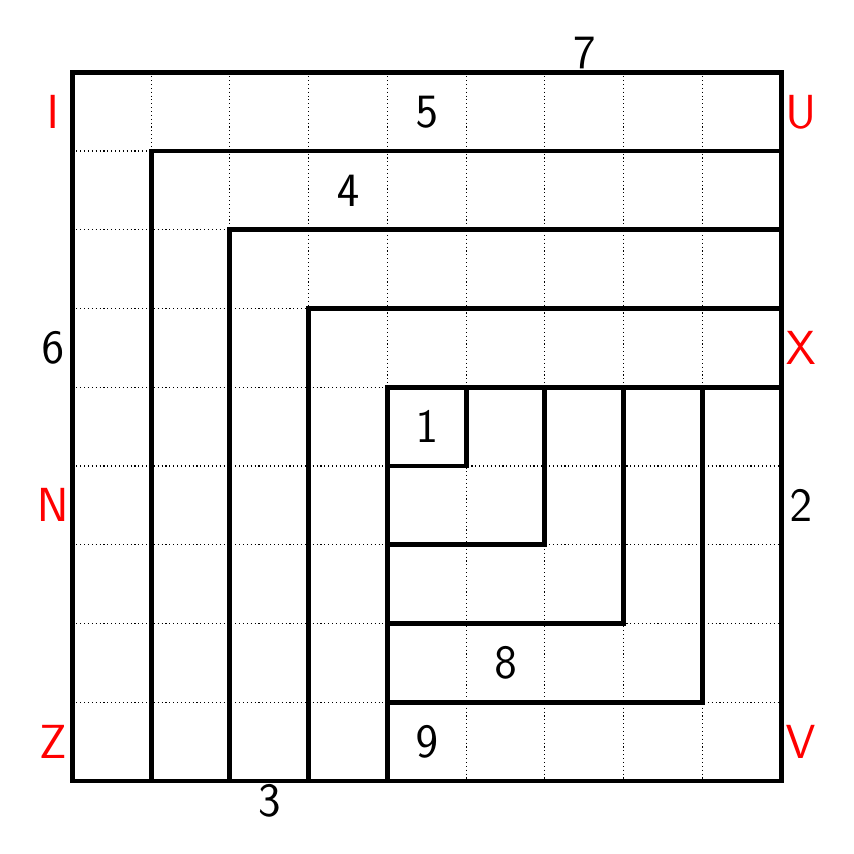
\begin{tikzpicture}
\drawthick (0,8)--++(0,1)--++(9,0)--++(0,-1)--++(-8,0)--++(0,-8)--++(-1,0)--cycle;
    \drawthick (1,7)--++(0,1)--++(8,0)--++(0,-1)--++(-7,0)--++(0,-7)--++(-1,0)--cycle;
    \drawthick (2,6)--++(0,1)--++(7,0)--++(0,-1)--++(-6,0)--++(0,-6)--++(-1,0)--cycle;
    \drawthick (3,5)--++(0,1)--++(6,0)--++(0,-1)--++(-5,0)--++(0,-5)--++(-1,0)--cycle;
    \drawthick (8,0)--++(-4,0)--++(0,1)--++(4,0)--++(0,4)--++(1,0)--++(0,-5)--cycle;
    \drawthick (7,1)--++(-3,0)--++(0,1)--++(3,0)--++(0,3)--++(1,0)--++(0,-4)--cycle;
    \drawthick (6,2)--++(-2,0)--++(0,1)--++(2,0)--++(0,2)--++(1,0)--++(0,-3)--cycle;
    \drawthick (5,3)--++(-1,0)--++(0,1)--++(1,0)--++(0,1)--++(1,0)--++(0,-2)--cycle;\drawgriddotted{9}
\numbersquare{1}{5}{5}\numbersquare{9}{5}{1}\numbersquare{8}{6}{2}\numbersquare{4}{4}{8}\numbersquare{5}{5}{9}\numbersquare{3}{3.0}{0.25}\numbersquare{2}{9.75}{4.0}\numbersquare{6}{0.25}{6.0}\numbersquare{7}{7.0}{9.75}\numbersquare{\textcolor{red}{I}}{0.25}{9.0}\numbersquare{\textcolor{red}{N}}{0.25}{4.0}\numbersquare{\textcolor{red}{Z}}{0.25}{1.0}\numbersquare{\textcolor{red}{V}}{9.75}{1.0}\numbersquare{\textcolor{red}{X}}{9.75}{6.0}\numbersquare{\textcolor{red}{U}}{9.75}{9.0}\end{tikzpicture}}
\vspace{1pc}\noindent{\large \texttt{\string{1:1, 2:$\sqcup$, 3:$\sqcup$, 4:$\sqcup$, 5:$\sqcup$, 6:$\sqcup$, 7:$\sqcup$, 8:$\sqcup$, 9:5\string}}}

\medskip\noindent{\large \texttt{hook 4 is too small for digit 8}}

\clearpage\resizebox{29.5pc}{!}{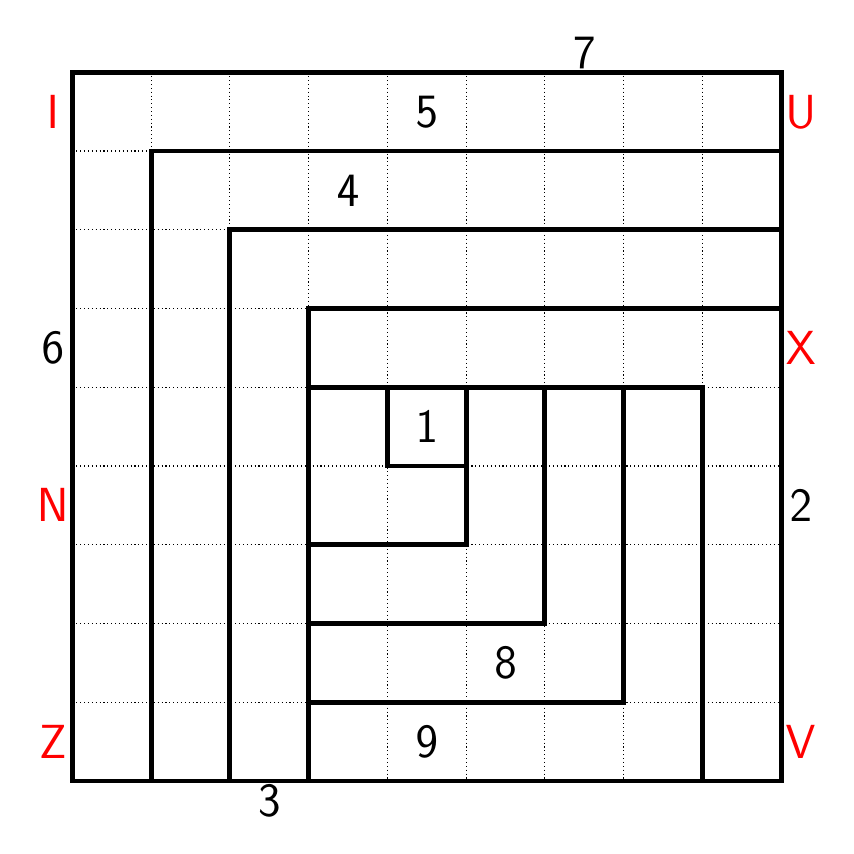
\begin{tikzpicture}
\drawthick (0,8)--++(0,1)--++(9,0)--++(0,-1)--++(-8,0)--++(0,-8)--++(-1,0)--cycle;
    \drawthick (1,7)--++(0,1)--++(8,0)--++(0,-1)--++(-7,0)--++(0,-7)--++(-1,0)--cycle;
    \drawthick (2,6)--++(0,1)--++(7,0)--++(0,-1)--++(-6,0)--++(0,-6)--++(-1,0)--cycle;
    \drawthick (8,5)--++(-5,0)--++(0,1)--++(6,0)--++(0,-6)--++(-1,0)--cycle;
    \drawthick (7,0)--++(-4,0)--++(0,1)--++(4,0)--++(0,4)--++(1,0)--++(0,-5)--cycle;
    \drawthick (6,1)--++(-3,0)--++(0,1)--++(3,0)--++(0,3)--++(1,0)--++(0,-4)--cycle;
    \drawthick (5,2)--++(-2,0)--++(0,1)--++(2,0)--++(0,2)--++(1,0)--++(0,-3)--cycle;
    \drawthick (3,3)--++(0,2)--++(1,0)--++(0,-1)--++(1,0)--++(0,-1)--cycle;\drawgriddotted{9}
\numbersquare{1}{5}{5}\numbersquare{9}{5}{1}\numbersquare{8}{6}{2}\numbersquare{4}{4}{8}\numbersquare{5}{5}{9}\numbersquare{3}{3.0}{0.25}\numbersquare{2}{9.75}{4.0}\numbersquare{6}{0.25}{6.0}\numbersquare{7}{7.0}{9.75}\numbersquare{\textcolor{red}{I}}{0.25}{9.0}\numbersquare{\textcolor{red}{N}}{0.25}{4.0}\numbersquare{\textcolor{red}{Z}}{0.25}{1.0}\numbersquare{\textcolor{red}{V}}{9.75}{1.0}\numbersquare{\textcolor{red}{X}}{9.75}{6.0}\numbersquare{\textcolor{red}{U}}{9.75}{9.0}\end{tikzpicture}}
\vspace{1pc}\noindent{\large \texttt{\string{1:1, 2:$\sqcup$, 3:$\sqcup$, 4:$\sqcup$, 5:$\sqcup$, 6:$\sqcup$, 7:$\sqcup$, 8:$\sqcup$, 9:5\string}}}

\medskip\noindent{\large \texttt{hook 4 is too small for digit 8}}

\clearpage\resizebox{29.5pc}{!}{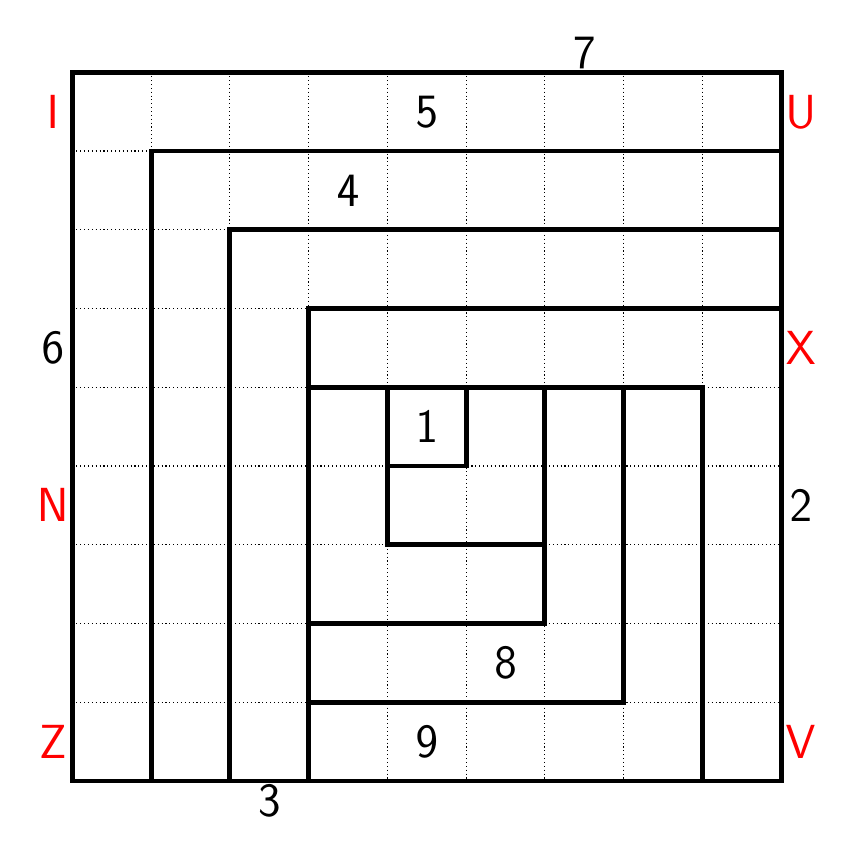
\begin{tikzpicture}
\drawthick (0,8)--++(0,1)--++(9,0)--++(0,-1)--++(-8,0)--++(0,-8)--++(-1,0)--cycle;
    \drawthick (1,7)--++(0,1)--++(8,0)--++(0,-1)--++(-7,0)--++(0,-7)--++(-1,0)--cycle;
    \drawthick (2,6)--++(0,1)--++(7,0)--++(0,-1)--++(-6,0)--++(0,-6)--++(-1,0)--cycle;
    \drawthick (8,5)--++(-5,0)--++(0,1)--++(6,0)--++(0,-6)--++(-1,0)--cycle;
    \drawthick (7,0)--++(-4,0)--++(0,1)--++(4,0)--++(0,4)--++(1,0)--++(0,-5)--cycle;
    \drawthick (6,1)--++(-3,0)--++(0,1)--++(3,0)--++(0,3)--++(1,0)--++(0,-4)--cycle;
    \drawthick (3,2)--++(0,3)--++(1,0)--++(0,-2)--++(2,0)--++(0,-1)--cycle;
    \drawthick (5,3)--++(-1,0)--++(0,1)--++(1,0)--++(0,1)--++(1,0)--++(0,-2)--cycle;\drawgriddotted{9}
\numbersquare{1}{5}{5}\numbersquare{9}{5}{1}\numbersquare{8}{6}{2}\numbersquare{4}{4}{8}\numbersquare{5}{5}{9}\numbersquare{3}{3.0}{0.25}\numbersquare{2}{9.75}{4.0}\numbersquare{6}{0.25}{6.0}\numbersquare{7}{7.0}{9.75}\numbersquare{\textcolor{red}{I}}{0.25}{9.0}\numbersquare{\textcolor{red}{N}}{0.25}{4.0}\numbersquare{\textcolor{red}{Z}}{0.25}{1.0}\numbersquare{\textcolor{red}{V}}{9.75}{1.0}\numbersquare{\textcolor{red}{X}}{9.75}{6.0}\numbersquare{\textcolor{red}{U}}{9.75}{9.0}\end{tikzpicture}}
\vspace{1pc}\noindent{\large \texttt{\string{1:1, 2:$\sqcup$, 3:$\sqcup$, 4:$\sqcup$, 5:$\sqcup$, 6:$\sqcup$, 7:$\sqcup$, 8:$\sqcup$, 9:5\string}}}

\medskip\noindent{\large \texttt{hook 4 is too small for digit 8}}

\clearpage\resizebox{29.5pc}{!}{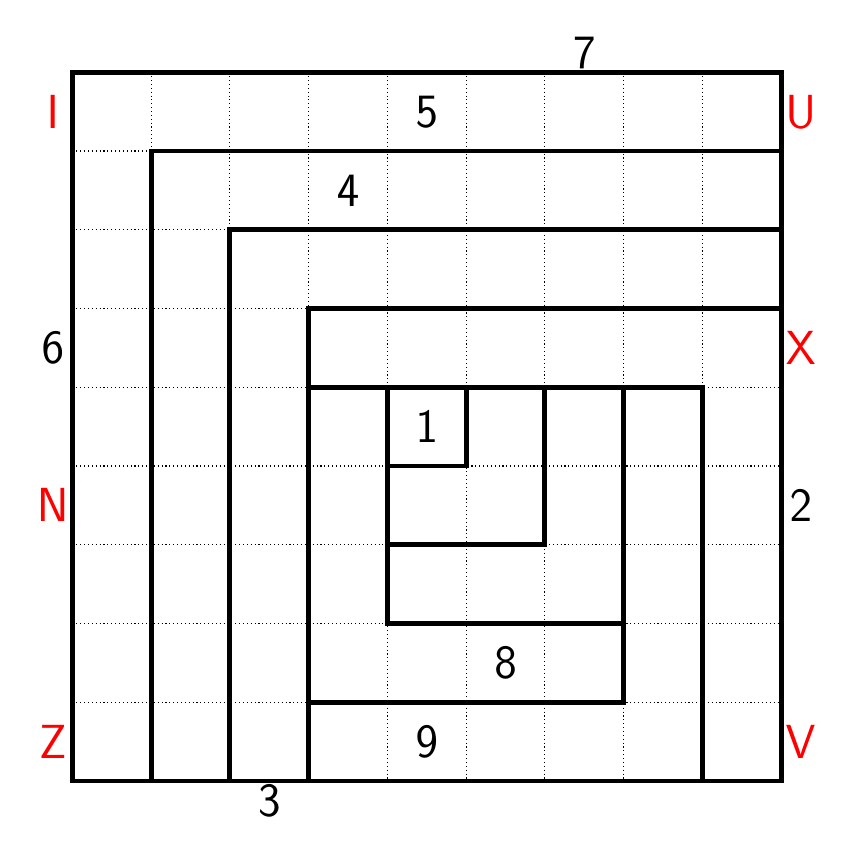
\begin{tikzpicture}
\drawthick (0,8)--++(0,1)--++(9,0)--++(0,-1)--++(-8,0)--++(0,-8)--++(-1,0)--cycle;
    \drawthick (1,7)--++(0,1)--++(8,0)--++(0,-1)--++(-7,0)--++(0,-7)--++(-1,0)--cycle;
    \drawthick (2,6)--++(0,1)--++(7,0)--++(0,-1)--++(-6,0)--++(0,-6)--++(-1,0)--cycle;
    \drawthick (8,5)--++(-5,0)--++(0,1)--++(6,0)--++(0,-6)--++(-1,0)--cycle;
    \drawthick (7,0)--++(-4,0)--++(0,1)--++(4,0)--++(0,4)--++(1,0)--++(0,-5)--cycle;
    \drawthick (3,1)--++(0,4)--++(1,0)--++(0,-3)--++(3,0)--++(0,-1)--cycle;
    \drawthick (6,2)--++(-2,0)--++(0,1)--++(2,0)--++(0,2)--++(1,0)--++(0,-3)--cycle;
    \drawthick (5,3)--++(-1,0)--++(0,1)--++(1,0)--++(0,1)--++(1,0)--++(0,-2)--cycle;\drawgriddotted{9}
\numbersquare{1}{5}{5}\numbersquare{9}{5}{1}\numbersquare{8}{6}{2}\numbersquare{4}{4}{8}\numbersquare{5}{5}{9}\numbersquare{3}{3.0}{0.25}\numbersquare{2}{9.75}{4.0}\numbersquare{6}{0.25}{6.0}\numbersquare{7}{7.0}{9.75}\numbersquare{\textcolor{red}{I}}{0.25}{9.0}\numbersquare{\textcolor{red}{N}}{0.25}{4.0}\numbersquare{\textcolor{red}{Z}}{0.25}{1.0}\numbersquare{\textcolor{red}{V}}{9.75}{1.0}\numbersquare{\textcolor{red}{X}}{9.75}{6.0}\numbersquare{\textcolor{red}{U}}{9.75}{9.0}\end{tikzpicture}}
\vspace{1pc}\noindent{\large \texttt{\string{1:1, 2:$\sqcup$, 3:$\sqcup$, 4:$\sqcup$, 5:$\sqcup$, 6:$\sqcup$, 7:$\sqcup$, 8:$\sqcup$, 9:5\string}}}

\medskip\noindent{\large \texttt{hook 4 is too small for digit 8}}

\clearpage\resizebox{29.5pc}{!}{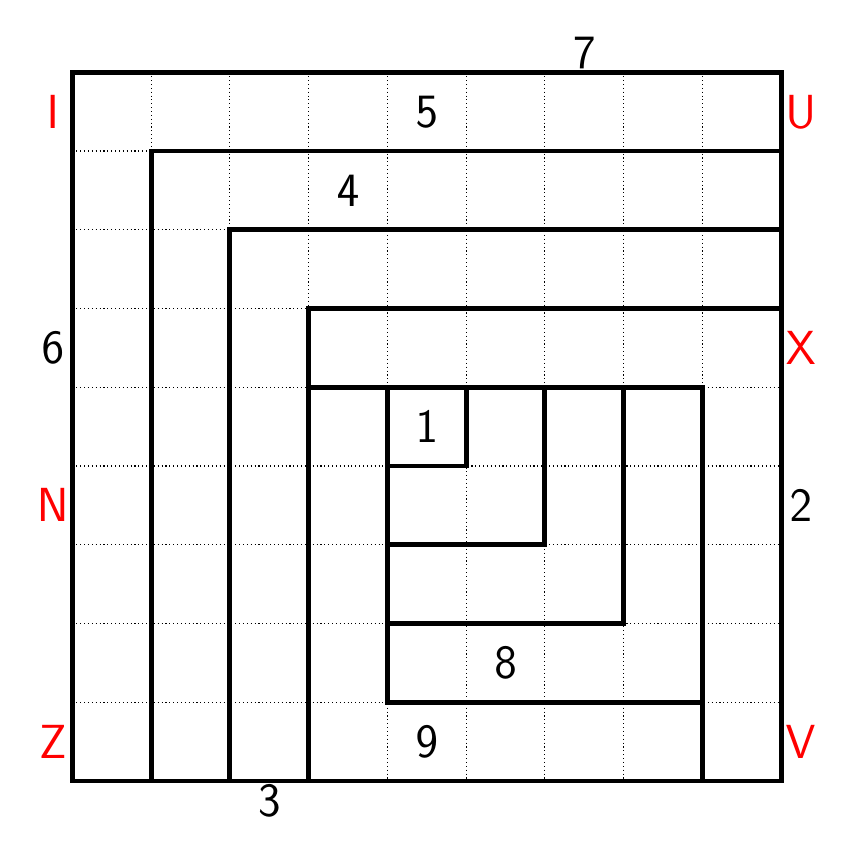
\begin{tikzpicture}
\drawthick (0,8)--++(0,1)--++(9,0)--++(0,-1)--++(-8,0)--++(0,-8)--++(-1,0)--cycle;
    \drawthick (1,7)--++(0,1)--++(8,0)--++(0,-1)--++(-7,0)--++(0,-7)--++(-1,0)--cycle;
    \drawthick (2,6)--++(0,1)--++(7,0)--++(0,-1)--++(-6,0)--++(0,-6)--++(-1,0)--cycle;
    \drawthick (8,5)--++(-5,0)--++(0,1)--++(6,0)--++(0,-6)--++(-1,0)--cycle;
    \drawthick (3,0)--++(0,5)--++(1,0)--++(0,-4)--++(4,0)--++(0,-1)--cycle;
    \drawthick (7,1)--++(-3,0)--++(0,1)--++(3,0)--++(0,3)--++(1,0)--++(0,-4)--cycle;
    \drawthick (6,2)--++(-2,0)--++(0,1)--++(2,0)--++(0,2)--++(1,0)--++(0,-3)--cycle;
    \drawthick (5,3)--++(-1,0)--++(0,1)--++(1,0)--++(0,1)--++(1,0)--++(0,-2)--cycle;\drawgriddotted{9}
\numbersquare{1}{5}{5}\numbersquare{9}{5}{1}\numbersquare{8}{6}{2}\numbersquare{4}{4}{8}\numbersquare{5}{5}{9}\numbersquare{3}{3.0}{0.25}\numbersquare{2}{9.75}{4.0}\numbersquare{6}{0.25}{6.0}\numbersquare{7}{7.0}{9.75}\numbersquare{\textcolor{red}{I}}{0.25}{9.0}\numbersquare{\textcolor{red}{N}}{0.25}{4.0}\numbersquare{\textcolor{red}{Z}}{0.25}{1.0}\numbersquare{\textcolor{red}{V}}{9.75}{1.0}\numbersquare{\textcolor{red}{X}}{9.75}{6.0}\numbersquare{\textcolor{red}{U}}{9.75}{9.0}\end{tikzpicture}}
\vspace{1pc}\noindent{\large \texttt{\string{1:1, 2:$\sqcup$, 3:$\sqcup$, 4:$\sqcup$, 5:$\sqcup$, 6:$\sqcup$, 7:$\sqcup$, 8:$\sqcup$, 9:5\string}}}

\medskip\noindent{\large \texttt{hook 4 is too small for digit 8}}

\clearpage\resizebox{29.5pc}{!}{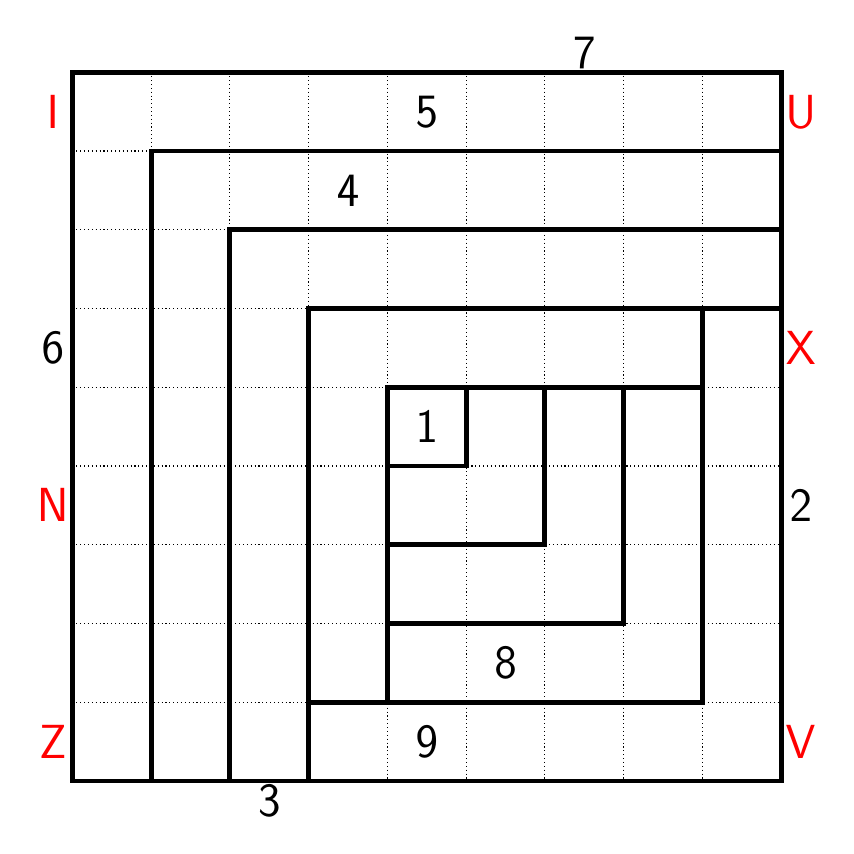
\begin{tikzpicture}
\drawthick (0,8)--++(0,1)--++(9,0)--++(0,-1)--++(-8,0)--++(0,-8)--++(-1,0)--cycle;
    \drawthick (1,7)--++(0,1)--++(8,0)--++(0,-1)--++(-7,0)--++(0,-7)--++(-1,0)--cycle;
    \drawthick (2,6)--++(0,1)--++(7,0)--++(0,-1)--++(-6,0)--++(0,-6)--++(-1,0)--cycle;
    \drawthick (8,0)--++(-5,0)--++(0,1)--++(5,0)--++(0,5)--++(1,0)--++(0,-6)--cycle;
    \drawthick (3,5)--++(0,1)--++(5,0)--++(0,-1)--++(-4,0)--++(0,-4)--++(-1,0)--cycle;
    \drawthick (7,1)--++(-3,0)--++(0,1)--++(3,0)--++(0,3)--++(1,0)--++(0,-4)--cycle;
    \drawthick (6,2)--++(-2,0)--++(0,1)--++(2,0)--++(0,2)--++(1,0)--++(0,-3)--cycle;
    \drawthick (5,3)--++(-1,0)--++(0,1)--++(1,0)--++(0,1)--++(1,0)--++(0,-2)--cycle;\drawgriddotted{9}
\numbersquare{1}{5}{5}\numbersquare{9}{5}{1}\numbersquare{8}{6}{2}\numbersquare{4}{4}{8}\numbersquare{5}{5}{9}\numbersquare{3}{3.0}{0.25}\numbersquare{2}{9.75}{4.0}\numbersquare{6}{0.25}{6.0}\numbersquare{7}{7.0}{9.75}\numbersquare{\textcolor{red}{I}}{0.25}{9.0}\numbersquare{\textcolor{red}{N}}{0.25}{4.0}\numbersquare{\textcolor{red}{Z}}{0.25}{1.0}\numbersquare{\textcolor{red}{V}}{9.75}{1.0}\numbersquare{\textcolor{red}{X}}{9.75}{6.0}\numbersquare{\textcolor{red}{U}}{9.75}{9.0}\end{tikzpicture}}
\vspace{1pc}\noindent{\large \texttt{\string{1:1, 2:$\sqcup$, 3:$\sqcup$, 4:$\sqcup$, 5:$\sqcup$, 6:$\sqcup$, 7:$\sqcup$, 8:$\sqcup$, 9:6\string}}}

\medskip\noindent{\large \texttt{hook 4 is too small for digit 8}}

\clearpage\resizebox{29.5pc}{!}{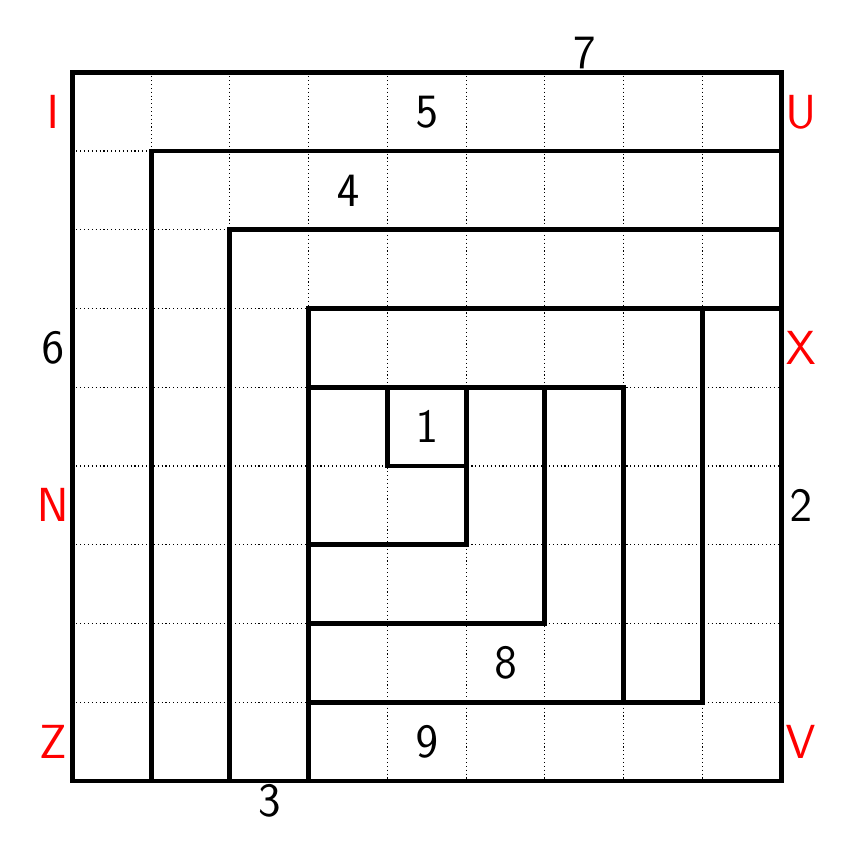
\begin{tikzpicture}
\drawthick (0,8)--++(0,1)--++(9,0)--++(0,-1)--++(-8,0)--++(0,-8)--++(-1,0)--cycle;
    \drawthick (1,7)--++(0,1)--++(8,0)--++(0,-1)--++(-7,0)--++(0,-7)--++(-1,0)--cycle;
    \drawthick (2,6)--++(0,1)--++(7,0)--++(0,-1)--++(-6,0)--++(0,-6)--++(-1,0)--cycle;
    \drawthick (8,0)--++(-5,0)--++(0,1)--++(5,0)--++(0,5)--++(1,0)--++(0,-6)--cycle;
    \drawthick (7,5)--++(-4,0)--++(0,1)--++(5,0)--++(0,-5)--++(-1,0)--cycle;
    \drawthick (6,1)--++(-3,0)--++(0,1)--++(3,0)--++(0,3)--++(1,0)--++(0,-4)--cycle;
    \drawthick (5,2)--++(-2,0)--++(0,1)--++(2,0)--++(0,2)--++(1,0)--++(0,-3)--cycle;
    \drawthick (3,3)--++(0,2)--++(1,0)--++(0,-1)--++(1,0)--++(0,-1)--cycle;\drawgriddotted{9}
\numbersquare{1}{5}{5}\numbersquare{9}{5}{1}\numbersquare{8}{6}{2}\numbersquare{4}{4}{8}\numbersquare{5}{5}{9}\numbersquare{3}{3.0}{0.25}\numbersquare{2}{9.75}{4.0}\numbersquare{6}{0.25}{6.0}\numbersquare{7}{7.0}{9.75}\numbersquare{\textcolor{red}{I}}{0.25}{9.0}\numbersquare{\textcolor{red}{N}}{0.25}{4.0}\numbersquare{\textcolor{red}{Z}}{0.25}{1.0}\numbersquare{\textcolor{red}{V}}{9.75}{1.0}\numbersquare{\textcolor{red}{X}}{9.75}{6.0}\numbersquare{\textcolor{red}{U}}{9.75}{9.0}\end{tikzpicture}}
\vspace{1pc}\noindent{\large \texttt{\string{1:1, 2:$\sqcup$, 3:$\sqcup$, 4:$\sqcup$, 5:$\sqcup$, 6:$\sqcup$, 7:$\sqcup$, 8:$\sqcup$, 9:6\string}}}

\medskip\noindent{\large \texttt{hook 4 is too small for digit 8}}

\clearpage\resizebox{29.5pc}{!}{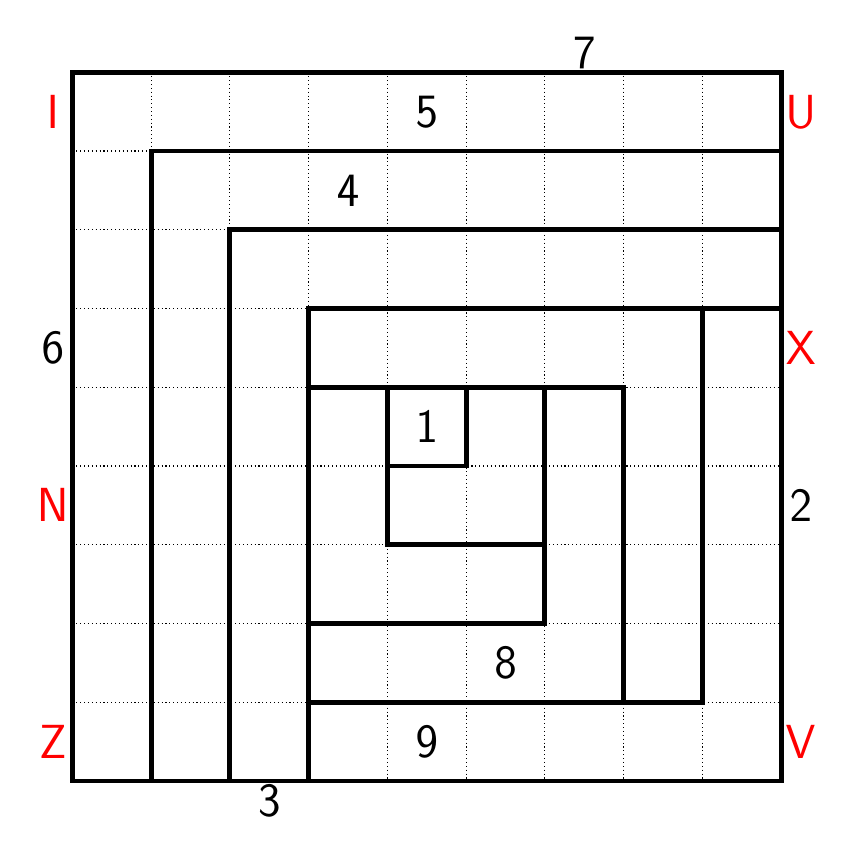
\begin{tikzpicture}
\drawthick (0,8)--++(0,1)--++(9,0)--++(0,-1)--++(-8,0)--++(0,-8)--++(-1,0)--cycle;
    \drawthick (1,7)--++(0,1)--++(8,0)--++(0,-1)--++(-7,0)--++(0,-7)--++(-1,0)--cycle;
    \drawthick (2,6)--++(0,1)--++(7,0)--++(0,-1)--++(-6,0)--++(0,-6)--++(-1,0)--cycle;
    \drawthick (8,0)--++(-5,0)--++(0,1)--++(5,0)--++(0,5)--++(1,0)--++(0,-6)--cycle;
    \drawthick (7,5)--++(-4,0)--++(0,1)--++(5,0)--++(0,-5)--++(-1,0)--cycle;
    \drawthick (6,1)--++(-3,0)--++(0,1)--++(3,0)--++(0,3)--++(1,0)--++(0,-4)--cycle;
    \drawthick (3,2)--++(0,3)--++(1,0)--++(0,-2)--++(2,0)--++(0,-1)--cycle;
    \drawthick (5,3)--++(-1,0)--++(0,1)--++(1,0)--++(0,1)--++(1,0)--++(0,-2)--cycle;\drawgriddotted{9}
\numbersquare{1}{5}{5}\numbersquare{9}{5}{1}\numbersquare{8}{6}{2}\numbersquare{4}{4}{8}\numbersquare{5}{5}{9}\numbersquare{3}{3.0}{0.25}\numbersquare{2}{9.75}{4.0}\numbersquare{6}{0.25}{6.0}\numbersquare{7}{7.0}{9.75}\numbersquare{\textcolor{red}{I}}{0.25}{9.0}\numbersquare{\textcolor{red}{N}}{0.25}{4.0}\numbersquare{\textcolor{red}{Z}}{0.25}{1.0}\numbersquare{\textcolor{red}{V}}{9.75}{1.0}\numbersquare{\textcolor{red}{X}}{9.75}{6.0}\numbersquare{\textcolor{red}{U}}{9.75}{9.0}\end{tikzpicture}}
\vspace{1pc}\noindent{\large \texttt{\string{1:1, 2:$\sqcup$, 3:$\sqcup$, 4:$\sqcup$, 5:$\sqcup$, 6:$\sqcup$, 7:$\sqcup$, 8:$\sqcup$, 9:6\string}}}

\medskip\noindent{\large \texttt{hook 4 is too small for digit 8}}

\clearpage\resizebox{29.5pc}{!}{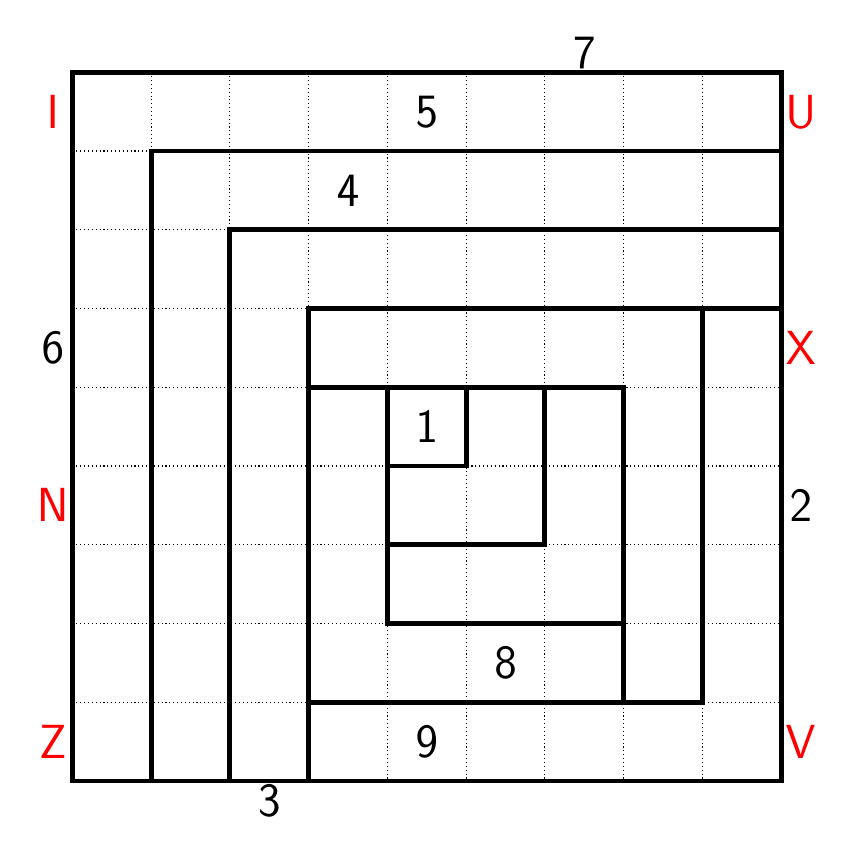
\begin{tikzpicture}
\drawthick (0,8)--++(0,1)--++(9,0)--++(0,-1)--++(-8,0)--++(0,-8)--++(-1,0)--cycle;
    \drawthick (1,7)--++(0,1)--++(8,0)--++(0,-1)--++(-7,0)--++(0,-7)--++(-1,0)--cycle;
    \drawthick (2,6)--++(0,1)--++(7,0)--++(0,-1)--++(-6,0)--++(0,-6)--++(-1,0)--cycle;
    \drawthick (8,0)--++(-5,0)--++(0,1)--++(5,0)--++(0,5)--++(1,0)--++(0,-6)--cycle;
    \drawthick (7,5)--++(-4,0)--++(0,1)--++(5,0)--++(0,-5)--++(-1,0)--cycle;
    \drawthick (3,1)--++(0,4)--++(1,0)--++(0,-3)--++(3,0)--++(0,-1)--cycle;
    \drawthick (6,2)--++(-2,0)--++(0,1)--++(2,0)--++(0,2)--++(1,0)--++(0,-3)--cycle;
    \drawthick (5,3)--++(-1,0)--++(0,1)--++(1,0)--++(0,1)--++(1,0)--++(0,-2)--cycle;\drawgriddotted{9}
\numbersquare{1}{5}{5}\numbersquare{9}{5}{1}\numbersquare{8}{6}{2}\numbersquare{4}{4}{8}\numbersquare{5}{5}{9}\numbersquare{3}{3.0}{0.25}\numbersquare{2}{9.75}{4.0}\numbersquare{6}{0.25}{6.0}\numbersquare{7}{7.0}{9.75}\numbersquare{\textcolor{red}{I}}{0.25}{9.0}\numbersquare{\textcolor{red}{N}}{0.25}{4.0}\numbersquare{\textcolor{red}{Z}}{0.25}{1.0}\numbersquare{\textcolor{red}{V}}{9.75}{1.0}\numbersquare{\textcolor{red}{X}}{9.75}{6.0}\numbersquare{\textcolor{red}{U}}{9.75}{9.0}\end{tikzpicture}}
\vspace{1pc}\noindent{\large \texttt{\string{1:1, 2:$\sqcup$, 3:$\sqcup$, 4:$\sqcup$, 5:$\sqcup$, 6:$\sqcup$, 7:$\sqcup$, 8:$\sqcup$, 9:6\string}}}

\medskip\noindent{\large \texttt{hook 4 is too small for digit 8}}

\clearpage\resizebox{29.5pc}{!}{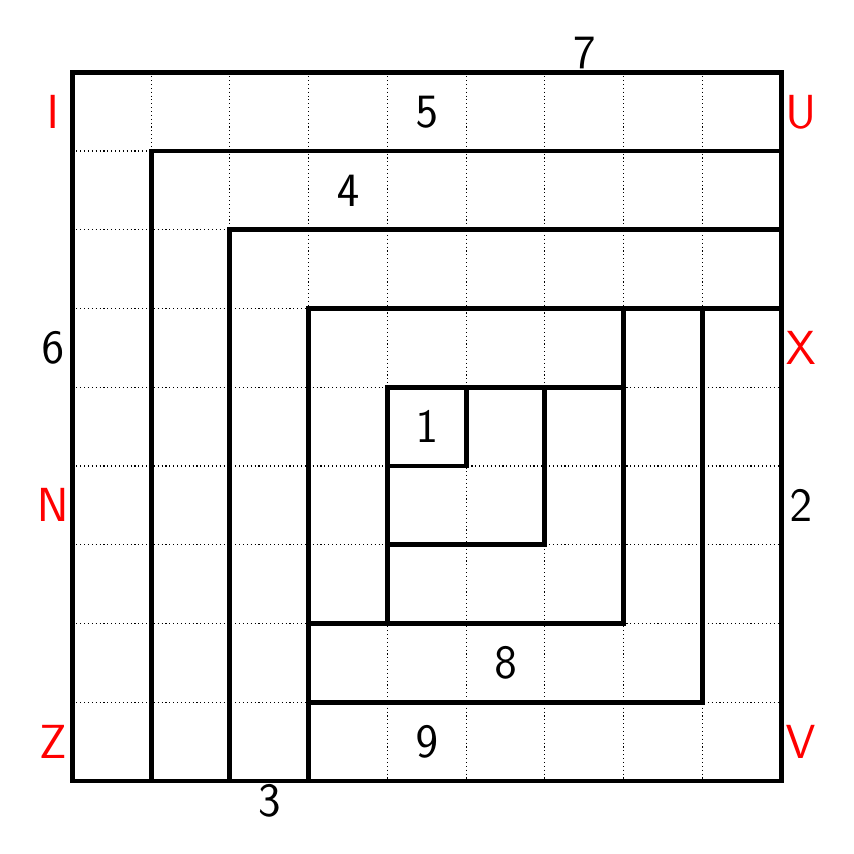
\begin{tikzpicture}
\drawthick (0,8)--++(0,1)--++(9,0)--++(0,-1)--++(-8,0)--++(0,-8)--++(-1,0)--cycle;
    \drawthick (1,7)--++(0,1)--++(8,0)--++(0,-1)--++(-7,0)--++(0,-7)--++(-1,0)--cycle;
    \drawthick (2,6)--++(0,1)--++(7,0)--++(0,-1)--++(-6,0)--++(0,-6)--++(-1,0)--cycle;
    \drawthick (8,0)--++(-5,0)--++(0,1)--++(5,0)--++(0,5)--++(1,0)--++(0,-6)--cycle;
    \drawthick (7,1)--++(-4,0)--++(0,1)--++(4,0)--++(0,4)--++(1,0)--++(0,-5)--cycle;
    \drawthick (3,5)--++(0,1)--++(4,0)--++(0,-1)--++(-3,0)--++(0,-3)--++(-1,0)--cycle;
    \drawthick (6,2)--++(-2,0)--++(0,1)--++(2,0)--++(0,2)--++(1,0)--++(0,-3)--cycle;
    \drawthick (5,3)--++(-1,0)--++(0,1)--++(1,0)--++(0,1)--++(1,0)--++(0,-2)--cycle;\drawgriddotted{9}
\numbersquare{1}{5}{5}\numbersquare{9}{5}{1}\numbersquare{8}{6}{2}\numbersquare{4}{4}{8}\numbersquare{5}{5}{9}\numbersquare{3}{3.0}{0.25}\numbersquare{2}{9.75}{4.0}\numbersquare{6}{0.25}{6.0}\numbersquare{7}{7.0}{9.75}\numbersquare{\textcolor{red}{I}}{0.25}{9.0}\numbersquare{\textcolor{red}{N}}{0.25}{4.0}\numbersquare{\textcolor{red}{Z}}{0.25}{1.0}\numbersquare{\textcolor{red}{V}}{9.75}{1.0}\numbersquare{\textcolor{red}{X}}{9.75}{6.0}\numbersquare{\textcolor{red}{U}}{9.75}{9.0}\end{tikzpicture}}
\vspace{1pc}\noindent{\large \texttt{\string{1:1, 2:[2, 3], 3:7, 4:8, 5:9, 6:4, 7:[], 8:5, 9:6\string}}}

\medskip\noindent{\large \texttt{digit(s) 7 cannot be assigned to any hook}}

\clearpage\resizebox{29.5pc}{!}{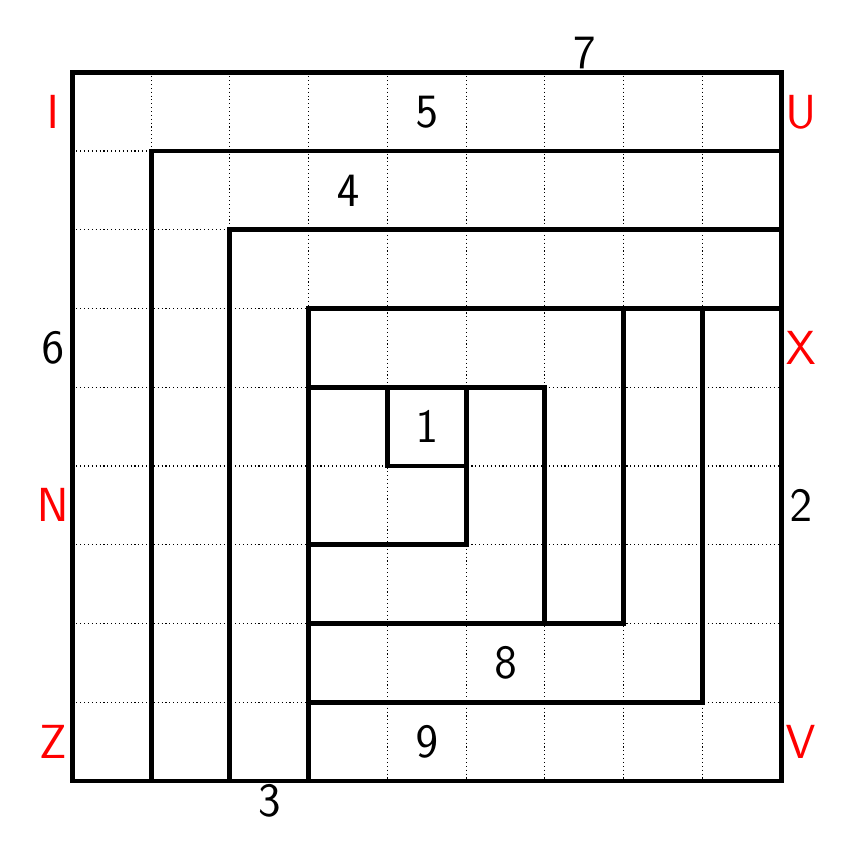
\begin{tikzpicture}
\drawthick (0,8)--++(0,1)--++(9,0)--++(0,-1)--++(-8,0)--++(0,-8)--++(-1,0)--cycle;
    \drawthick (1,7)--++(0,1)--++(8,0)--++(0,-1)--++(-7,0)--++(0,-7)--++(-1,0)--cycle;
    \drawthick (2,6)--++(0,1)--++(7,0)--++(0,-1)--++(-6,0)--++(0,-6)--++(-1,0)--cycle;
    \drawthick (8,0)--++(-5,0)--++(0,1)--++(5,0)--++(0,5)--++(1,0)--++(0,-6)--cycle;
    \drawthick (7,1)--++(-4,0)--++(0,1)--++(4,0)--++(0,4)--++(1,0)--++(0,-5)--cycle;
    \drawthick (6,5)--++(-3,0)--++(0,1)--++(4,0)--++(0,-4)--++(-1,0)--cycle;
    \drawthick (5,2)--++(-2,0)--++(0,1)--++(2,0)--++(0,2)--++(1,0)--++(0,-3)--cycle;
    \drawthick (3,3)--++(0,2)--++(1,0)--++(0,-1)--++(1,0)--++(0,-1)--cycle;\drawgriddotted{9}
\numbersquare{1}{5}{5}\numbersquare{9}{5}{1}\numbersquare{8}{6}{2}\numbersquare{4}{4}{8}\numbersquare{5}{5}{9}\numbersquare{3}{3.0}{0.25}\numbersquare{2}{9.75}{4.0}\numbersquare{6}{0.25}{6.0}\numbersquare{7}{7.0}{9.75}\numbersquare{\textcolor{red}{I}}{0.25}{9.0}\numbersquare{\textcolor{red}{N}}{0.25}{4.0}\numbersquare{\textcolor{red}{Z}}{0.25}{1.0}\numbersquare{\textcolor{red}{V}}{9.75}{1.0}\numbersquare{\textcolor{red}{X}}{9.75}{6.0}\numbersquare{\textcolor{red}{U}}{9.75}{9.0}\end{tikzpicture}}
\vspace{1pc}\noindent{\large \texttt{\string{1:1, 2:[2, 3], 3:7, 4:8, 5:9, 6:4, 7:[], 8:5, 9:6\string}}}

\medskip\noindent{\large \texttt{digit(s) 7 cannot be assigned to any hook}}

\clearpage\resizebox{29.5pc}{!}{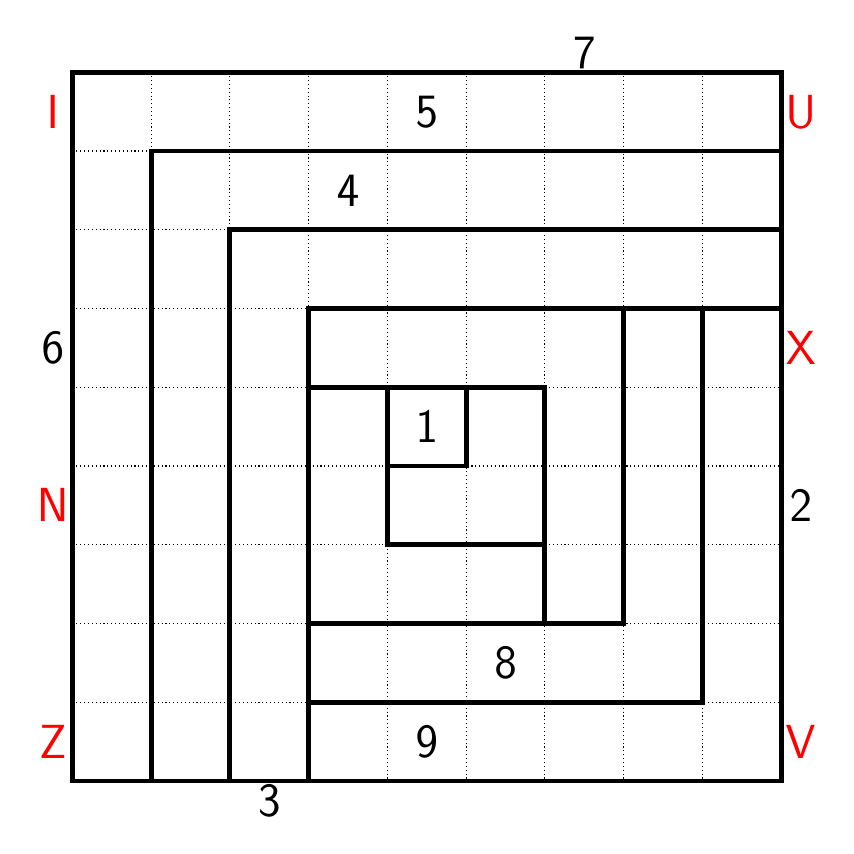
\begin{tikzpicture}
\drawthick (0,8)--++(0,1)--++(9,0)--++(0,-1)--++(-8,0)--++(0,-8)--++(-1,0)--cycle;
    \drawthick (1,7)--++(0,1)--++(8,0)--++(0,-1)--++(-7,0)--++(0,-7)--++(-1,0)--cycle;
    \drawthick (2,6)--++(0,1)--++(7,0)--++(0,-1)--++(-6,0)--++(0,-6)--++(-1,0)--cycle;
    \drawthick (8,0)--++(-5,0)--++(0,1)--++(5,0)--++(0,5)--++(1,0)--++(0,-6)--cycle;
    \drawthick (7,1)--++(-4,0)--++(0,1)--++(4,0)--++(0,4)--++(1,0)--++(0,-5)--cycle;
    \drawthick (6,5)--++(-3,0)--++(0,1)--++(4,0)--++(0,-4)--++(-1,0)--cycle;
    \drawthick (3,2)--++(0,3)--++(1,0)--++(0,-2)--++(2,0)--++(0,-1)--cycle;
    \drawthick (5,3)--++(-1,0)--++(0,1)--++(1,0)--++(0,1)--++(1,0)--++(0,-2)--cycle;\drawgriddotted{9}
\numbersquare{1}{5}{5}\numbersquare{9}{5}{1}\numbersquare{8}{6}{2}\numbersquare{4}{4}{8}\numbersquare{5}{5}{9}\numbersquare{3}{3.0}{0.25}\numbersquare{2}{9.75}{4.0}\numbersquare{6}{0.25}{6.0}\numbersquare{7}{7.0}{9.75}\numbersquare{\textcolor{red}{I}}{0.25}{9.0}\numbersquare{\textcolor{red}{N}}{0.25}{4.0}\numbersquare{\textcolor{red}{Z}}{0.25}{1.0}\numbersquare{\textcolor{red}{V}}{9.75}{1.0}\numbersquare{\textcolor{red}{X}}{9.75}{6.0}\numbersquare{\textcolor{red}{U}}{9.75}{9.0}\end{tikzpicture}}
\vspace{1pc}\noindent{\large \texttt{\string{1:1, 2:[2, 3], 3:7, 4:8, 5:9, 6:4, 7:[], 8:5, 9:6\string}}}

\medskip\noindent{\large \texttt{digit(s) 7 cannot be assigned to any hook}}

\clearpage\resizebox{29.5pc}{!}{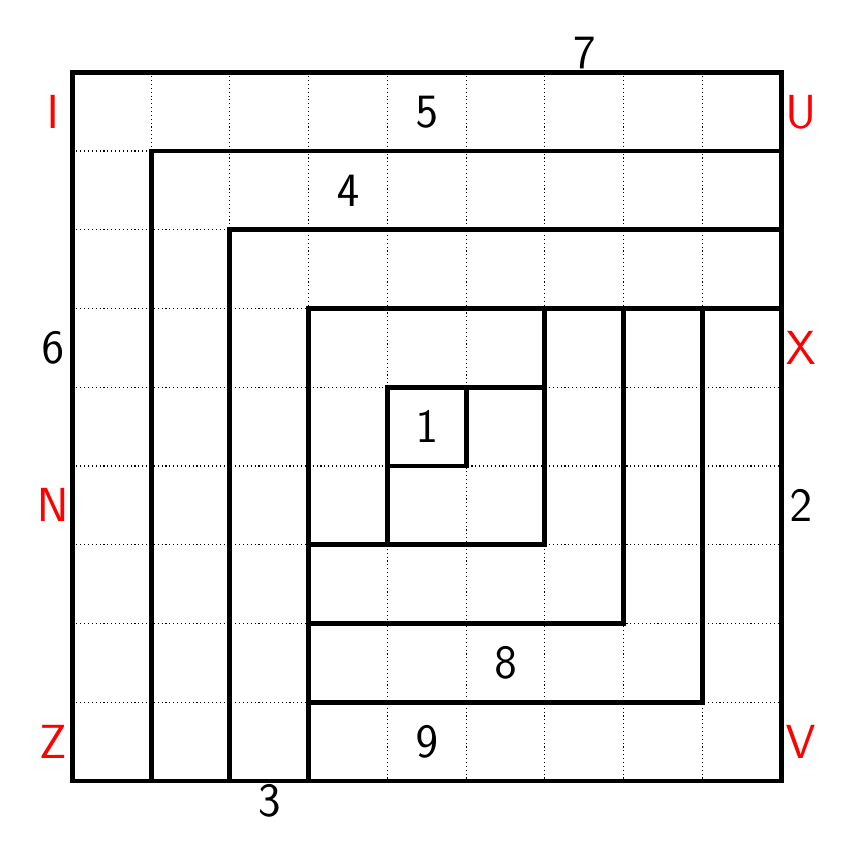
\begin{tikzpicture}
\drawthick (0,8)--++(0,1)--++(9,0)--++(0,-1)--++(-8,0)--++(0,-8)--++(-1,0)--cycle;
    \drawthick (1,7)--++(0,1)--++(8,0)--++(0,-1)--++(-7,0)--++(0,-7)--++(-1,0)--cycle;
    \drawthick (2,6)--++(0,1)--++(7,0)--++(0,-1)--++(-6,0)--++(0,-6)--++(-1,0)--cycle;
    \drawthick (8,0)--++(-5,0)--++(0,1)--++(5,0)--++(0,5)--++(1,0)--++(0,-6)--cycle;
    \drawthick (7,1)--++(-4,0)--++(0,1)--++(4,0)--++(0,4)--++(1,0)--++(0,-5)--cycle;
    \drawthick (6,2)--++(-3,0)--++(0,1)--++(3,0)--++(0,3)--++(1,0)--++(0,-4)--cycle;
    \drawthick (3,5)--++(0,1)--++(3,0)--++(0,-1)--++(-2,0)--++(0,-2)--++(-1,0)--cycle;
    \drawthick (5,3)--++(-1,0)--++(0,1)--++(1,0)--++(0,1)--++(1,0)--++(0,-2)--cycle;\drawgriddotted{9}
\numbersquare{1}{5}{5}\numbersquare{9}{5}{1}\numbersquare{8}{6}{2}\numbersquare{4}{4}{8}\numbersquare{5}{5}{9}\numbersquare{3}{3.0}{0.25}\numbersquare{2}{9.75}{4.0}\numbersquare{6}{0.25}{6.0}\numbersquare{7}{7.0}{9.75}\numbersquare{\textcolor{red}{I}}{0.25}{9.0}\numbersquare{\textcolor{red}{N}}{0.25}{4.0}\numbersquare{\textcolor{red}{Z}}{0.25}{1.0}\numbersquare{\textcolor{red}{V}}{9.75}{1.0}\numbersquare{\textcolor{red}{X}}{9.75}{6.0}\numbersquare{\textcolor{red}{U}}{9.75}{9.0}\end{tikzpicture}}
\vspace{1pc}\noindent{\large \texttt{\string{1:1, 2:[2, 3], 3:7, 4:8, 5:9, 6:4, 7:[], 8:5, 9:6\string}}}

\medskip\noindent{\large \texttt{digit(s) 7 cannot be assigned to any hook}}

\clearpage\resizebox{29.5pc}{!}{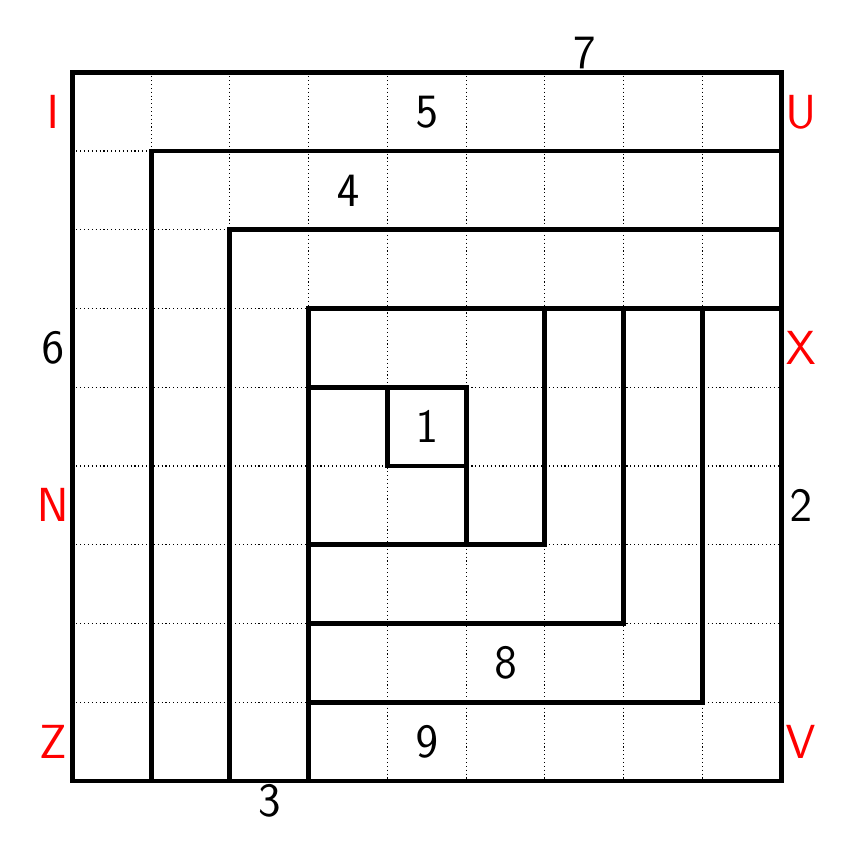
\begin{tikzpicture}
\drawthick (0,8)--++(0,1)--++(9,0)--++(0,-1)--++(-8,0)--++(0,-8)--++(-1,0)--cycle;
    \drawthick (1,7)--++(0,1)--++(8,0)--++(0,-1)--++(-7,0)--++(0,-7)--++(-1,0)--cycle;
    \drawthick (2,6)--++(0,1)--++(7,0)--++(0,-1)--++(-6,0)--++(0,-6)--++(-1,0)--cycle;
    \drawthick (8,0)--++(-5,0)--++(0,1)--++(5,0)--++(0,5)--++(1,0)--++(0,-6)--cycle;
    \drawthick (7,1)--++(-4,0)--++(0,1)--++(4,0)--++(0,4)--++(1,0)--++(0,-5)--cycle;
    \drawthick (6,2)--++(-3,0)--++(0,1)--++(3,0)--++(0,3)--++(1,0)--++(0,-4)--cycle;
    \drawthick (5,5)--++(-2,0)--++(0,1)--++(3,0)--++(0,-3)--++(-1,0)--cycle;
    \drawthick (3,3)--++(0,2)--++(1,0)--++(0,-1)--++(1,0)--++(0,-1)--cycle;\drawgriddotted{9}
\numbersquare{1}{5}{5}\numbersquare{9}{5}{1}\numbersquare{8}{6}{2}\numbersquare{4}{4}{8}\numbersquare{5}{5}{9}\numbersquare{3}{3.0}{0.25}\numbersquare{2}{9.75}{4.0}\numbersquare{6}{0.25}{6.0}\numbersquare{7}{7.0}{9.75}\numbersquare{\textcolor{red}{I}}{0.25}{9.0}\numbersquare{\textcolor{red}{N}}{0.25}{4.0}\numbersquare{\textcolor{red}{Z}}{0.25}{1.0}\numbersquare{\textcolor{red}{V}}{9.75}{1.0}\numbersquare{\textcolor{red}{X}}{9.75}{6.0}\numbersquare{\textcolor{red}{U}}{9.75}{9.0}\end{tikzpicture}}
\vspace{1pc}\noindent{\large \texttt{\string{1:1, 2:[2, 3], 3:7, 4:8, 5:9, 6:4, 7:[], 8:5, 9:6\string}}}

\medskip\noindent{\large \texttt{digit(s) 7 cannot be assigned to any hook}}

\clearpage\resizebox{29.5pc}{!}{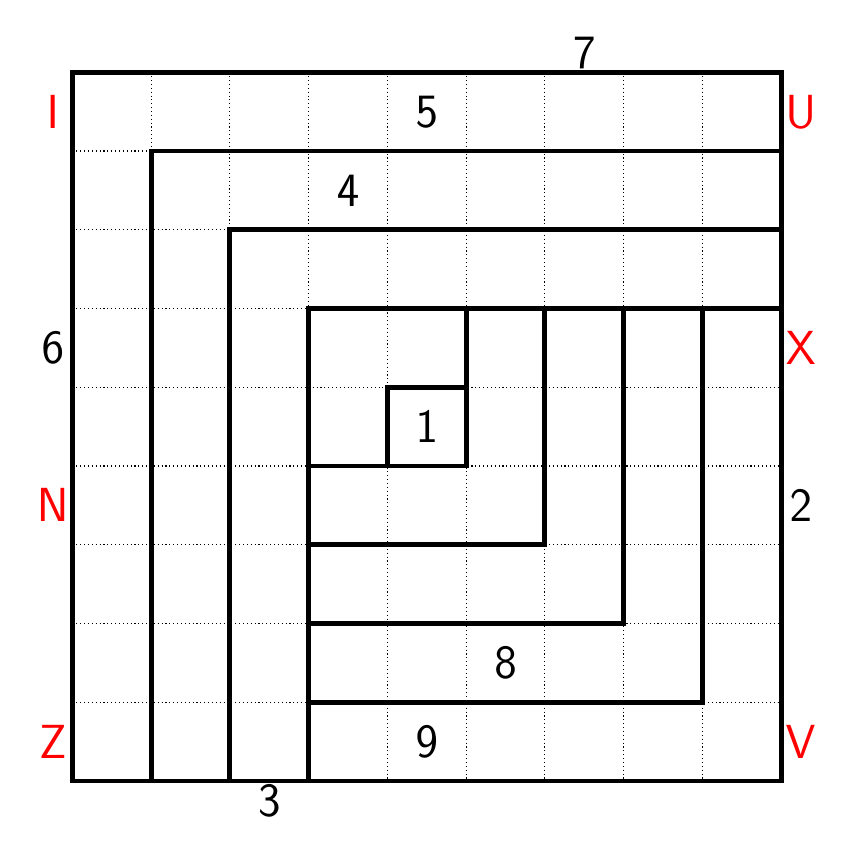
\begin{tikzpicture}
\drawthick (0,8)--++(0,1)--++(9,0)--++(0,-1)--++(-8,0)--++(0,-8)--++(-1,0)--cycle;
    \drawthick (1,7)--++(0,1)--++(8,0)--++(0,-1)--++(-7,0)--++(0,-7)--++(-1,0)--cycle;
    \drawthick (2,6)--++(0,1)--++(7,0)--++(0,-1)--++(-6,0)--++(0,-6)--++(-1,0)--cycle;
    \drawthick (8,0)--++(-5,0)--++(0,1)--++(5,0)--++(0,5)--++(1,0)--++(0,-6)--cycle;
    \drawthick (7,1)--++(-4,0)--++(0,1)--++(4,0)--++(0,4)--++(1,0)--++(0,-5)--cycle;
    \drawthick (6,2)--++(-3,0)--++(0,1)--++(3,0)--++(0,3)--++(1,0)--++(0,-4)--cycle;
    \drawthick (5,3)--++(-2,0)--++(0,1)--++(2,0)--++(0,2)--++(1,0)--++(0,-3)--cycle;
    \drawthick (3,5)--++(0,1)--++(2,0)--++(0,-1)--++(-1,0)--++(0,-1)--++(-1,0)--cycle;\drawgriddotted{9}
\numbersquare{1}{5}{5}\numbersquare{9}{5}{1}\numbersquare{8}{6}{2}\numbersquare{4}{4}{8}\numbersquare{5}{5}{9}\numbersquare{3}{3.0}{0.25}\numbersquare{2}{9.75}{4.0}\numbersquare{6}{0.25}{6.0}\numbersquare{7}{7.0}{9.75}\numbersquare{\textcolor{red}{I}}{0.25}{9.0}\numbersquare{\textcolor{red}{N}}{0.25}{4.0}\numbersquare{\textcolor{red}{Z}}{0.25}{1.0}\numbersquare{\textcolor{red}{V}}{9.75}{1.0}\numbersquare{\textcolor{red}{X}}{9.75}{6.0}\numbersquare{\textcolor{red}{U}}{9.75}{9.0}\end{tikzpicture}}
\vspace{1pc}\noindent{\large \texttt{\string{1:1, 2:3, 3:7, 4:8, 5:9, 6:4, 7:[], 8:5, 9:6\string}}}

\medskip\noindent{\large \texttt{digit(s) 7 cannot be assigned to any hook}}

\clearpage\resizebox{29.5pc}{!}{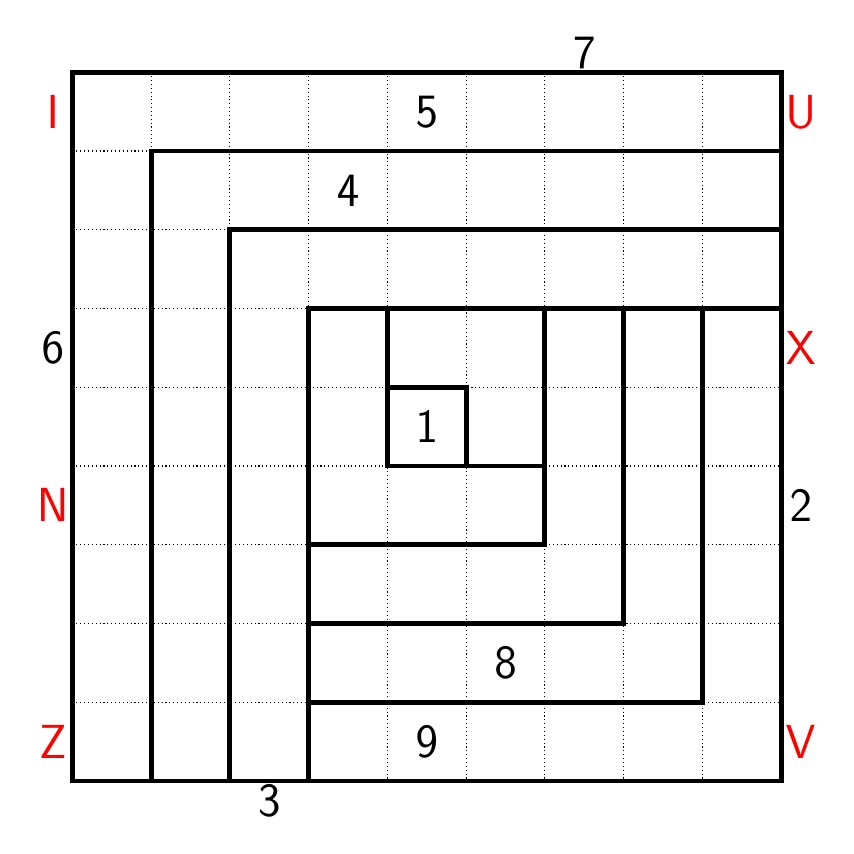
\begin{tikzpicture}
\drawthick (0,8)--++(0,1)--++(9,0)--++(0,-1)--++(-8,0)--++(0,-8)--++(-1,0)--cycle;
    \drawthick (1,7)--++(0,1)--++(8,0)--++(0,-1)--++(-7,0)--++(0,-7)--++(-1,0)--cycle;
    \drawthick (2,6)--++(0,1)--++(7,0)--++(0,-1)--++(-6,0)--++(0,-6)--++(-1,0)--cycle;
    \drawthick (8,0)--++(-5,0)--++(0,1)--++(5,0)--++(0,5)--++(1,0)--++(0,-6)--cycle;
    \drawthick (7,1)--++(-4,0)--++(0,1)--++(4,0)--++(0,4)--++(1,0)--++(0,-5)--cycle;
    \drawthick (6,2)--++(-3,0)--++(0,1)--++(3,0)--++(0,3)--++(1,0)--++(0,-4)--cycle;
    \drawthick (3,3)--++(0,3)--++(1,0)--++(0,-2)--++(2,0)--++(0,-1)--cycle;
    \drawthick (5,5)--++(-1,0)--++(0,1)--++(2,0)--++(0,-2)--++(-1,0)--cycle;\drawgriddotted{9}
\numbersquare{1}{5}{5}\numbersquare{9}{5}{1}\numbersquare{8}{6}{2}\numbersquare{4}{4}{8}\numbersquare{5}{5}{9}\numbersquare{3}{3.0}{0.25}\numbersquare{2}{9.75}{4.0}\numbersquare{6}{0.25}{6.0}\numbersquare{7}{7.0}{9.75}\numbersquare{\textcolor{red}{I}}{0.25}{9.0}\numbersquare{\textcolor{red}{N}}{0.25}{4.0}\numbersquare{\textcolor{red}{Z}}{0.25}{1.0}\numbersquare{\textcolor{red}{V}}{9.75}{1.0}\numbersquare{\textcolor{red}{X}}{9.75}{6.0}\numbersquare{\textcolor{red}{U}}{9.75}{9.0}\end{tikzpicture}}
\vspace{1pc}\noindent{\large \texttt{\string{1:1, 2:3, 3:7, 4:8, 5:9, 6:4, 7:[], 8:5, 9:6\string}}}

\medskip\noindent{\large \texttt{digit(s) 7 cannot be assigned to any hook}}

\clearpage\resizebox{29.5pc}{!}{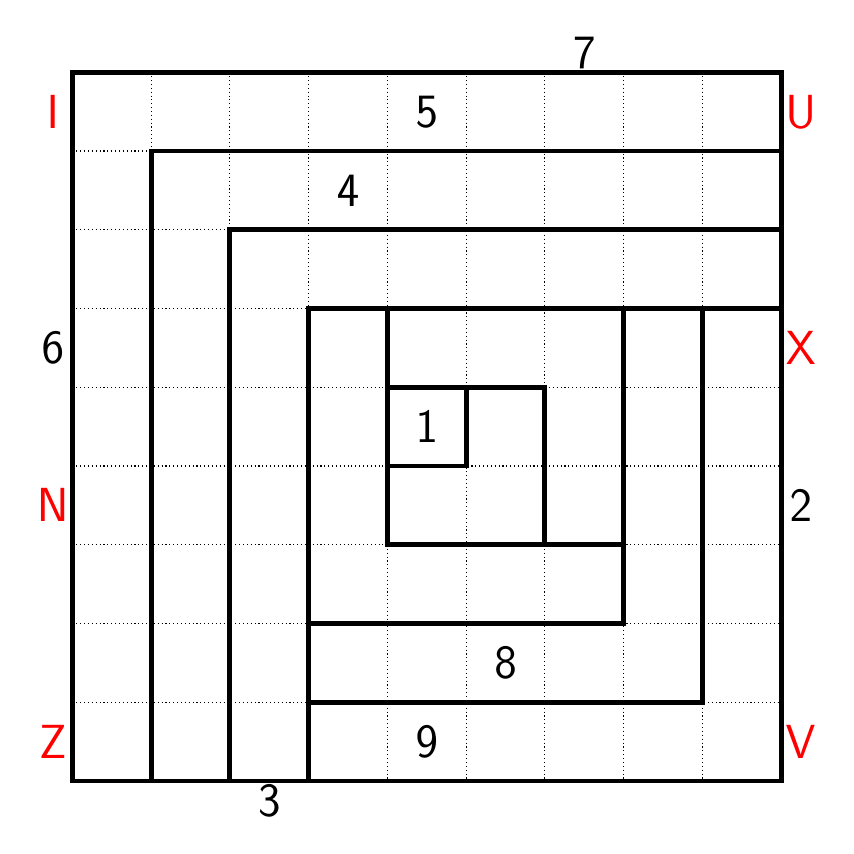
\begin{tikzpicture}
\drawthick (0,8)--++(0,1)--++(9,0)--++(0,-1)--++(-8,0)--++(0,-8)--++(-1,0)--cycle;
    \drawthick (1,7)--++(0,1)--++(8,0)--++(0,-1)--++(-7,0)--++(0,-7)--++(-1,0)--cycle;
    \drawthick (2,6)--++(0,1)--++(7,0)--++(0,-1)--++(-6,0)--++(0,-6)--++(-1,0)--cycle;
    \drawthick (8,0)--++(-5,0)--++(0,1)--++(5,0)--++(0,5)--++(1,0)--++(0,-6)--cycle;
    \drawthick (7,1)--++(-4,0)--++(0,1)--++(4,0)--++(0,4)--++(1,0)--++(0,-5)--cycle;
    \drawthick (3,2)--++(0,4)--++(1,0)--++(0,-3)--++(3,0)--++(0,-1)--cycle;
    \drawthick (6,5)--++(-2,0)--++(0,1)--++(3,0)--++(0,-3)--++(-1,0)--cycle;
    \drawthick (5,3)--++(-1,0)--++(0,1)--++(1,0)--++(0,1)--++(1,0)--++(0,-2)--cycle;\drawgriddotted{9}
\numbersquare{1}{5}{5}\numbersquare{9}{5}{1}\numbersquare{8}{6}{2}\numbersquare{4}{4}{8}\numbersquare{5}{5}{9}\numbersquare{3}{3.0}{0.25}\numbersquare{2}{9.75}{4.0}\numbersquare{6}{0.25}{6.0}\numbersquare{7}{7.0}{9.75}\numbersquare{\textcolor{red}{I}}{0.25}{9.0}\numbersquare{\textcolor{red}{N}}{0.25}{4.0}\numbersquare{\textcolor{red}{Z}}{0.25}{1.0}\numbersquare{\textcolor{red}{V}}{9.75}{1.0}\numbersquare{\textcolor{red}{X}}{9.75}{6.0}\numbersquare{\textcolor{red}{U}}{9.75}{9.0}\end{tikzpicture}}
\vspace{1pc}\noindent{\large \texttt{\string{1:1, 2:[2, 3], 3:7, 4:8, 5:9, 6:4, 7:[], 8:5, 9:6\string}}}

\medskip\noindent{\large \texttt{digit(s) 7 cannot be assigned to any hook}}

\clearpage\resizebox{29.5pc}{!}{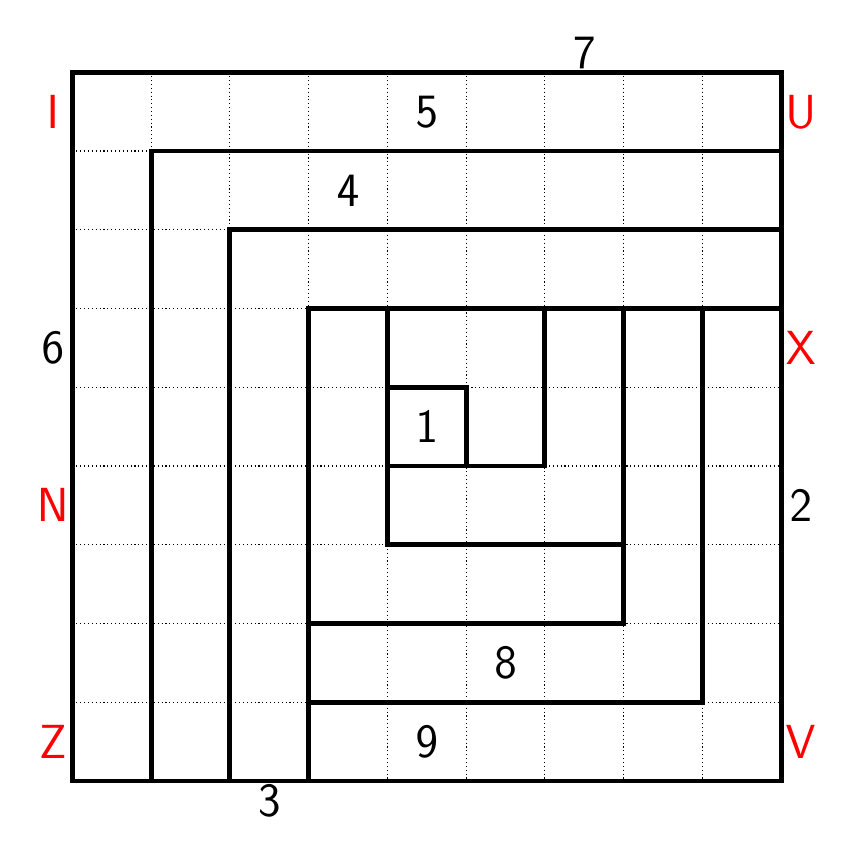
\begin{tikzpicture}
\drawthick (0,8)--++(0,1)--++(9,0)--++(0,-1)--++(-8,0)--++(0,-8)--++(-1,0)--cycle;
    \drawthick (1,7)--++(0,1)--++(8,0)--++(0,-1)--++(-7,0)--++(0,-7)--++(-1,0)--cycle;
    \drawthick (2,6)--++(0,1)--++(7,0)--++(0,-1)--++(-6,0)--++(0,-6)--++(-1,0)--cycle;
    \drawthick (8,0)--++(-5,0)--++(0,1)--++(5,0)--++(0,5)--++(1,0)--++(0,-6)--cycle;
    \drawthick (7,1)--++(-4,0)--++(0,1)--++(4,0)--++(0,4)--++(1,0)--++(0,-5)--cycle;
    \drawthick (3,2)--++(0,4)--++(1,0)--++(0,-3)--++(3,0)--++(0,-1)--cycle;
    \drawthick (6,3)--++(-2,0)--++(0,1)--++(2,0)--++(0,2)--++(1,0)--++(0,-3)--cycle;
    \drawthick (5,5)--++(-1,0)--++(0,1)--++(2,0)--++(0,-2)--++(-1,0)--cycle;\drawgriddotted{9}
\numbersquare{1}{5}{5}\numbersquare{9}{5}{1}\numbersquare{8}{6}{2}\numbersquare{4}{4}{8}\numbersquare{5}{5}{9}\numbersquare{3}{3.0}{0.25}\numbersquare{2}{9.75}{4.0}\numbersquare{6}{0.25}{6.0}\numbersquare{7}{7.0}{9.75}\numbersquare{\textcolor{red}{I}}{0.25}{9.0}\numbersquare{\textcolor{red}{N}}{0.25}{4.0}\numbersquare{\textcolor{red}{Z}}{0.25}{1.0}\numbersquare{\textcolor{red}{V}}{9.75}{1.0}\numbersquare{\textcolor{red}{X}}{9.75}{6.0}\numbersquare{\textcolor{red}{U}}{9.75}{9.0}\end{tikzpicture}}
\vspace{1pc}\noindent{\large \texttt{\string{1:1, 2:3, 3:7, 4:8, 5:9, 6:4, 7:[], 8:5, 9:6\string}}}

\medskip\noindent{\large \texttt{digit(s) 7 cannot be assigned to any hook}}

\clearpage\resizebox{29.5pc}{!}{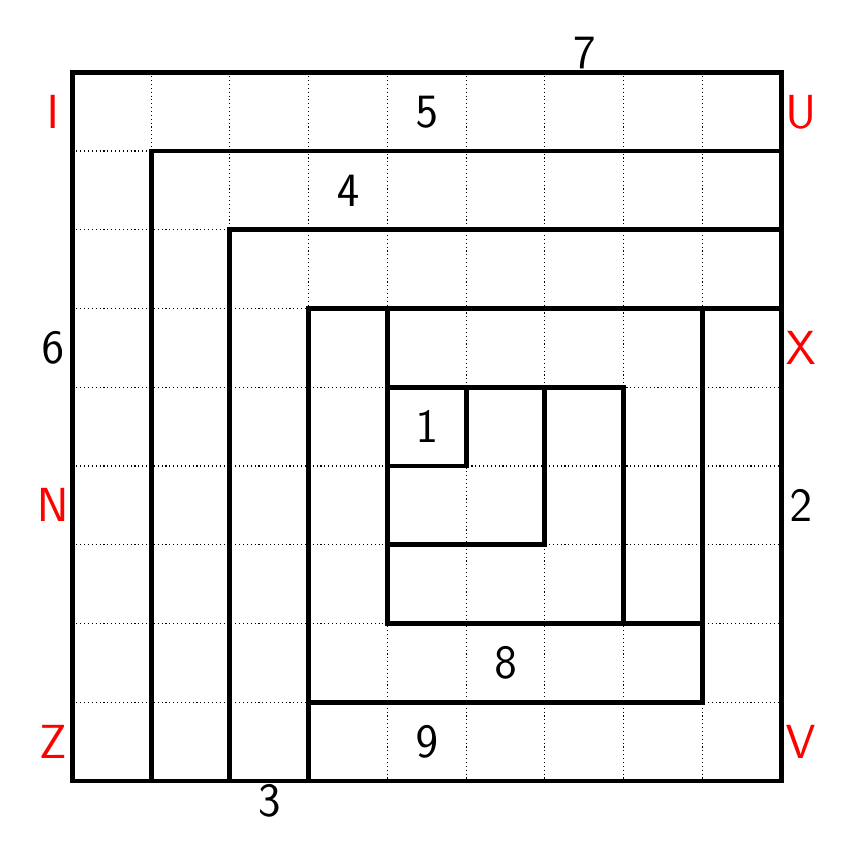
\begin{tikzpicture}
\drawthick (0,8)--++(0,1)--++(9,0)--++(0,-1)--++(-8,0)--++(0,-8)--++(-1,0)--cycle;
    \drawthick (1,7)--++(0,1)--++(8,0)--++(0,-1)--++(-7,0)--++(0,-7)--++(-1,0)--cycle;
    \drawthick (2,6)--++(0,1)--++(7,0)--++(0,-1)--++(-6,0)--++(0,-6)--++(-1,0)--cycle;
    \drawthick (8,0)--++(-5,0)--++(0,1)--++(5,0)--++(0,5)--++(1,0)--++(0,-6)--cycle;
    \drawthick (3,1)--++(0,5)--++(1,0)--++(0,-4)--++(4,0)--++(0,-1)--cycle;
    \drawthick (7,5)--++(-3,0)--++(0,1)--++(4,0)--++(0,-4)--++(-1,0)--cycle;
    \drawthick (6,2)--++(-2,0)--++(0,1)--++(2,0)--++(0,2)--++(1,0)--++(0,-3)--cycle;
    \drawthick (5,3)--++(-1,0)--++(0,1)--++(1,0)--++(0,1)--++(1,0)--++(0,-2)--cycle;\drawgriddotted{9}
\numbersquare{1}{5}{5}\numbersquare{9}{5}{1}\numbersquare{8}{6}{2}\numbersquare{4}{4}{8}\numbersquare{5}{5}{9}\numbersquare{3}{3.0}{0.25}\numbersquare{2}{9.75}{4.0}\numbersquare{6}{0.25}{6.0}\numbersquare{7}{7.0}{9.75}\numbersquare{\textcolor{red}{I}}{0.25}{9.0}\numbersquare{\textcolor{red}{N}}{0.25}{4.0}\numbersquare{\textcolor{red}{Z}}{0.25}{1.0}\numbersquare{\textcolor{red}{V}}{9.75}{1.0}\numbersquare{\textcolor{red}{X}}{9.75}{6.0}\numbersquare{\textcolor{red}{U}}{9.75}{9.0}\end{tikzpicture}}
\vspace{1pc}\noindent{\large \texttt{\string{1:1, 2:[2, 3], 3:7, 4:8, 5:9, 6:4, 7:[], 8:5, 9:6\string}}}

\medskip\noindent{\large \texttt{digit(s) 7 cannot be assigned to any hook}}

\clearpage\resizebox{29.5pc}{!}{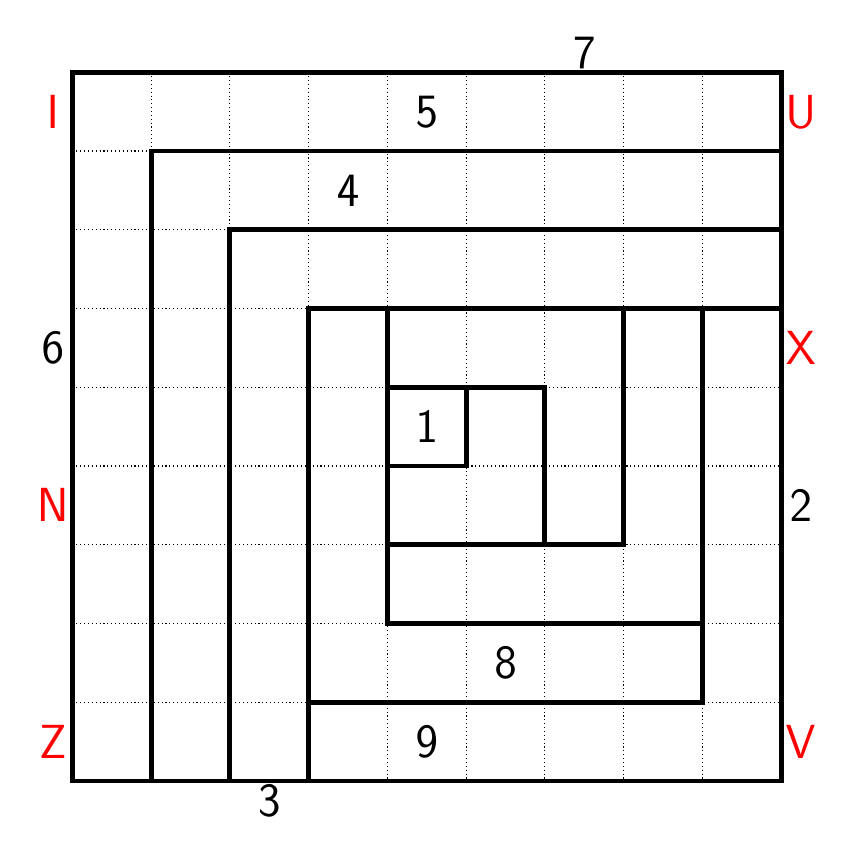
\begin{tikzpicture}
\drawthick (0,8)--++(0,1)--++(9,0)--++(0,-1)--++(-8,0)--++(0,-8)--++(-1,0)--cycle;
    \drawthick (1,7)--++(0,1)--++(8,0)--++(0,-1)--++(-7,0)--++(0,-7)--++(-1,0)--cycle;
    \drawthick (2,6)--++(0,1)--++(7,0)--++(0,-1)--++(-6,0)--++(0,-6)--++(-1,0)--cycle;
    \drawthick (8,0)--++(-5,0)--++(0,1)--++(5,0)--++(0,5)--++(1,0)--++(0,-6)--cycle;
    \drawthick (3,1)--++(0,5)--++(1,0)--++(0,-4)--++(4,0)--++(0,-1)--cycle;
    \drawthick (7,2)--++(-3,0)--++(0,1)--++(3,0)--++(0,3)--++(1,0)--++(0,-4)--cycle;
    \drawthick (6,5)--++(-2,0)--++(0,1)--++(3,0)--++(0,-3)--++(-1,0)--cycle;
    \drawthick (5,3)--++(-1,0)--++(0,1)--++(1,0)--++(0,1)--++(1,0)--++(0,-2)--cycle;\drawgriddotted{9}
\numbersquare{1}{5}{5}\numbersquare{9}{5}{1}\numbersquare{8}{6}{2}\numbersquare{4}{4}{8}\numbersquare{5}{5}{9}\numbersquare{3}{3.0}{0.25}\numbersquare{2}{9.75}{4.0}\numbersquare{6}{0.25}{6.0}\numbersquare{7}{7.0}{9.75}\numbersquare{\textcolor{red}{I}}{0.25}{9.0}\numbersquare{\textcolor{red}{N}}{0.25}{4.0}\numbersquare{\textcolor{red}{Z}}{0.25}{1.0}\numbersquare{\textcolor{red}{V}}{9.75}{1.0}\numbersquare{\textcolor{red}{X}}{9.75}{6.0}\numbersquare{\textcolor{red}{U}}{9.75}{9.0}\end{tikzpicture}}
\vspace{1pc}\noindent{\large \texttt{\string{1:1, 2:[2, 3], 3:7, 4:8, 5:9, 6:4, 7:[], 8:5, 9:6\string}}}

\medskip\noindent{\large \texttt{digit(s) 7 cannot be assigned to any hook}}

\clearpage\resizebox{29.5pc}{!}{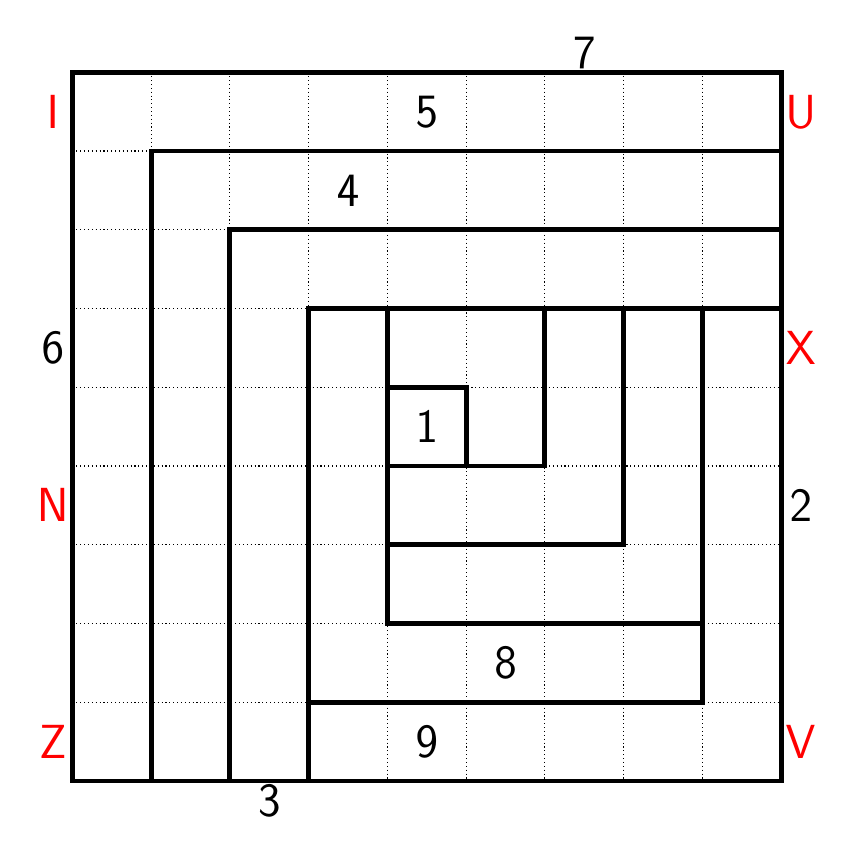
\begin{tikzpicture}
\drawthick (0,8)--++(0,1)--++(9,0)--++(0,-1)--++(-8,0)--++(0,-8)--++(-1,0)--cycle;
    \drawthick (1,7)--++(0,1)--++(8,0)--++(0,-1)--++(-7,0)--++(0,-7)--++(-1,0)--cycle;
    \drawthick (2,6)--++(0,1)--++(7,0)--++(0,-1)--++(-6,0)--++(0,-6)--++(-1,0)--cycle;
    \drawthick (8,0)--++(-5,0)--++(0,1)--++(5,0)--++(0,5)--++(1,0)--++(0,-6)--cycle;
    \drawthick (3,1)--++(0,5)--++(1,0)--++(0,-4)--++(4,0)--++(0,-1)--cycle;
    \drawthick (7,2)--++(-3,0)--++(0,1)--++(3,0)--++(0,3)--++(1,0)--++(0,-4)--cycle;
    \drawthick (6,3)--++(-2,0)--++(0,1)--++(2,0)--++(0,2)--++(1,0)--++(0,-3)--cycle;
    \drawthick (5,5)--++(-1,0)--++(0,1)--++(2,0)--++(0,-2)--++(-1,0)--cycle;\drawgriddotted{9}
\numbersquare{1}{5}{5}\numbersquare{9}{5}{1}\numbersquare{8}{6}{2}\numbersquare{4}{4}{8}\numbersquare{5}{5}{9}\numbersquare{3}{3.0}{0.25}\numbersquare{2}{9.75}{4.0}\numbersquare{6}{0.25}{6.0}\numbersquare{7}{7.0}{9.75}\numbersquare{\textcolor{red}{I}}{0.25}{9.0}\numbersquare{\textcolor{red}{N}}{0.25}{4.0}\numbersquare{\textcolor{red}{Z}}{0.25}{1.0}\numbersquare{\textcolor{red}{V}}{9.75}{1.0}\numbersquare{\textcolor{red}{X}}{9.75}{6.0}\numbersquare{\textcolor{red}{U}}{9.75}{9.0}\end{tikzpicture}}
\vspace{1pc}\noindent{\large \texttt{\string{1:1, 2:3, 3:7, 4:8, 5:9, 6:4, 7:[], 8:5, 9:6\string}}}

\medskip\noindent{\large \texttt{digit(s) 7 cannot be assigned to any hook}}

\clearpage\resizebox{29.5pc}{!}{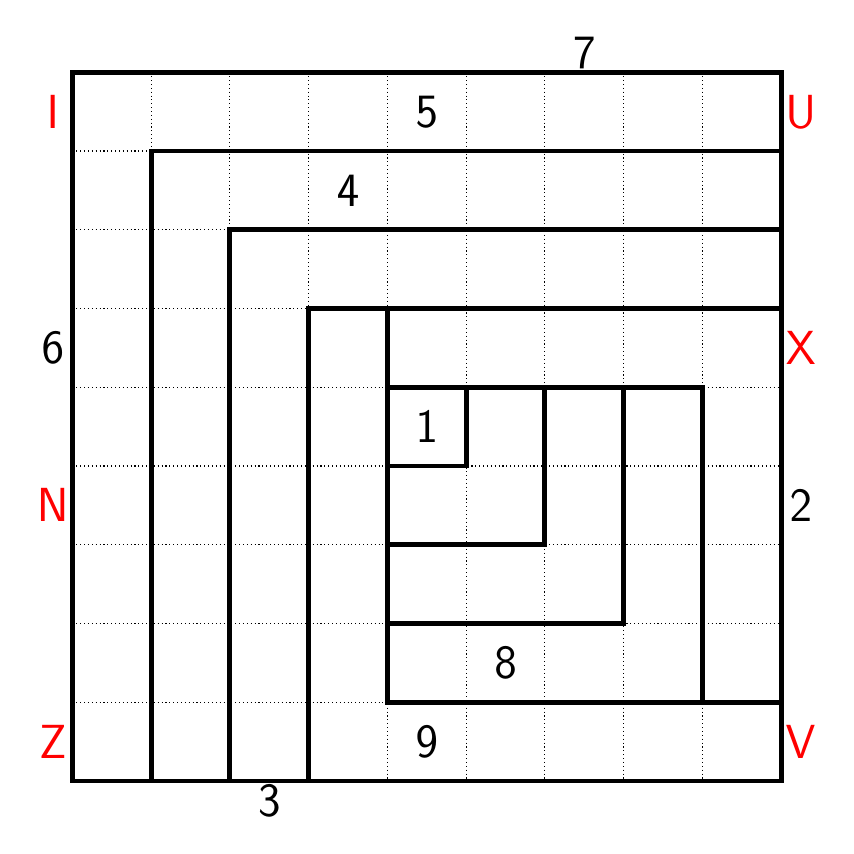
\begin{tikzpicture}
\drawthick (0,8)--++(0,1)--++(9,0)--++(0,-1)--++(-8,0)--++(0,-8)--++(-1,0)--cycle;
    \drawthick (1,7)--++(0,1)--++(8,0)--++(0,-1)--++(-7,0)--++(0,-7)--++(-1,0)--cycle;
    \drawthick (2,6)--++(0,1)--++(7,0)--++(0,-1)--++(-6,0)--++(0,-6)--++(-1,0)--cycle;
    \drawthick (3,0)--++(0,6)--++(1,0)--++(0,-5)--++(5,0)--++(0,-1)--cycle;
    \drawthick (8,5)--++(-4,0)--++(0,1)--++(5,0)--++(0,-5)--++(-1,0)--cycle;
    \drawthick (7,1)--++(-3,0)--++(0,1)--++(3,0)--++(0,3)--++(1,0)--++(0,-4)--cycle;
    \drawthick (6,2)--++(-2,0)--++(0,1)--++(2,0)--++(0,2)--++(1,0)--++(0,-3)--cycle;
    \drawthick (5,3)--++(-1,0)--++(0,1)--++(1,0)--++(0,1)--++(1,0)--++(0,-2)--cycle;\drawgriddotted{9}
\numbersquare{1}{5}{5}\numbersquare{9}{5}{1}\numbersquare{8}{6}{2}\numbersquare{4}{4}{8}\numbersquare{5}{5}{9}\numbersquare{3}{3.0}{0.25}\numbersquare{2}{9.75}{4.0}\numbersquare{6}{0.25}{6.0}\numbersquare{7}{7.0}{9.75}\numbersquare{\textcolor{red}{I}}{0.25}{9.0}\numbersquare{\textcolor{red}{N}}{0.25}{4.0}\numbersquare{\textcolor{red}{Z}}{0.25}{1.0}\numbersquare{\textcolor{red}{V}}{9.75}{1.0}\numbersquare{\textcolor{red}{X}}{9.75}{6.0}\numbersquare{\textcolor{red}{U}}{9.75}{9.0}\end{tikzpicture}}
\vspace{1pc}\noindent{\large \texttt{\string{1:1, 2:$\sqcup$, 3:$\sqcup$, 4:$\sqcup$, 5:$\sqcup$, 6:$\sqcup$, 7:$\sqcup$, 8:$\sqcup$, 9:6\string}}}

\medskip\noindent{\large \texttt{hook 4 is too small for digit 8}}

\clearpage\resizebox{29.5pc}{!}{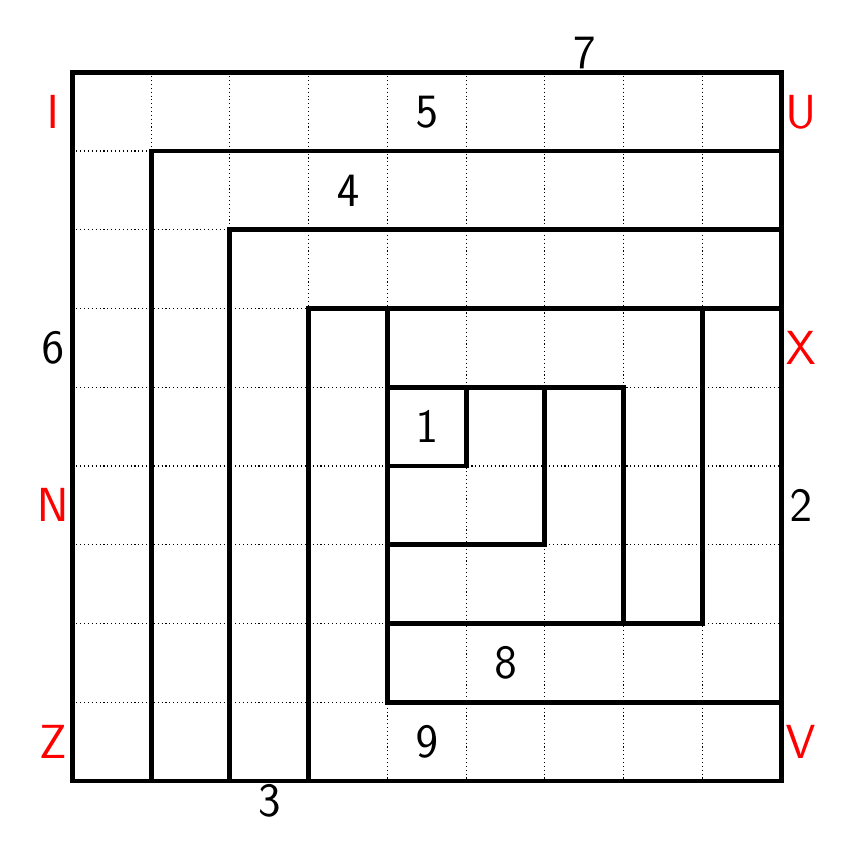
\begin{tikzpicture}
\drawthick (0,8)--++(0,1)--++(9,0)--++(0,-1)--++(-8,0)--++(0,-8)--++(-1,0)--cycle;
    \drawthick (1,7)--++(0,1)--++(8,0)--++(0,-1)--++(-7,0)--++(0,-7)--++(-1,0)--cycle;
    \drawthick (2,6)--++(0,1)--++(7,0)--++(0,-1)--++(-6,0)--++(0,-6)--++(-1,0)--cycle;
    \drawthick (3,0)--++(0,6)--++(1,0)--++(0,-5)--++(5,0)--++(0,-1)--cycle;
    \drawthick (8,1)--++(-4,0)--++(0,1)--++(4,0)--++(0,4)--++(1,0)--++(0,-5)--cycle;
    \drawthick (7,5)--++(-3,0)--++(0,1)--++(4,0)--++(0,-4)--++(-1,0)--cycle;
    \drawthick (6,2)--++(-2,0)--++(0,1)--++(2,0)--++(0,2)--++(1,0)--++(0,-3)--cycle;
    \drawthick (5,3)--++(-1,0)--++(0,1)--++(1,0)--++(0,1)--++(1,0)--++(0,-2)--cycle;\drawgriddotted{9}
\numbersquare{1}{5}{5}\numbersquare{9}{5}{1}\numbersquare{8}{6}{2}\numbersquare{4}{4}{8}\numbersquare{5}{5}{9}\numbersquare{3}{3.0}{0.25}\numbersquare{2}{9.75}{4.0}\numbersquare{6}{0.25}{6.0}\numbersquare{7}{7.0}{9.75}\numbersquare{\textcolor{red}{I}}{0.25}{9.0}\numbersquare{\textcolor{red}{N}}{0.25}{4.0}\numbersquare{\textcolor{red}{Z}}{0.25}{1.0}\numbersquare{\textcolor{red}{V}}{9.75}{1.0}\numbersquare{\textcolor{red}{X}}{9.75}{6.0}\numbersquare{\textcolor{red}{U}}{9.75}{9.0}\end{tikzpicture}}
\vspace{1pc}\noindent{\large \texttt{\string{1:1, 2:[2, 3], 3:7, 4:8, 5:9, 6:4, 7:[], 8:5, 9:6\string}}}

\medskip\noindent{\large \texttt{digit(s) 7 cannot be assigned to any hook}}

\clearpage\resizebox{29.5pc}{!}{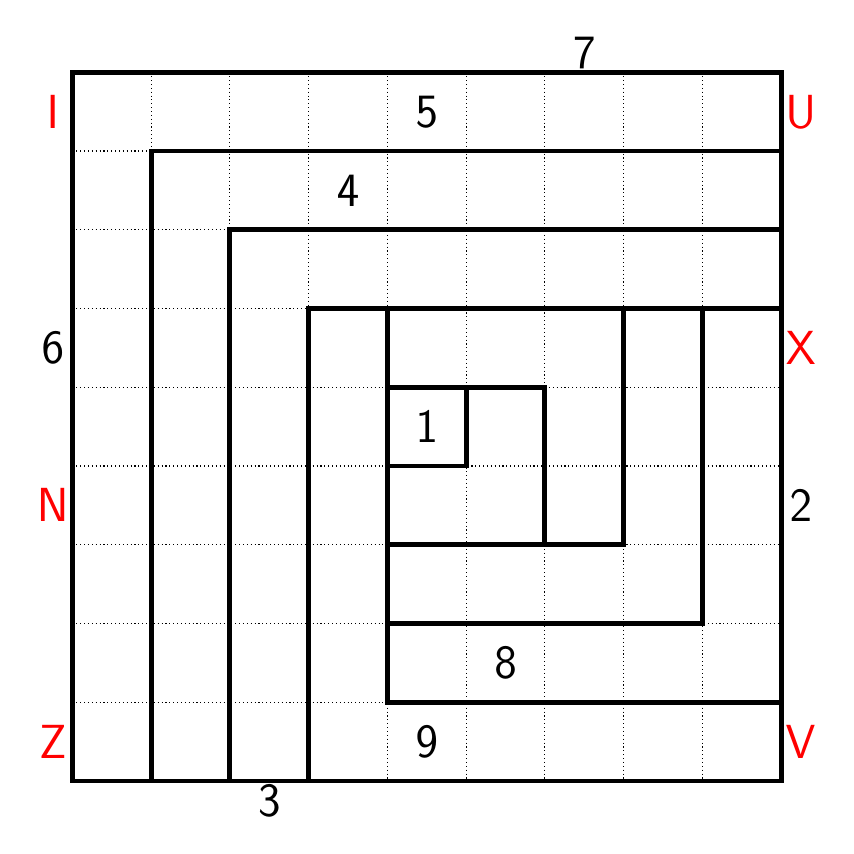
\begin{tikzpicture}
\drawthick (0,8)--++(0,1)--++(9,0)--++(0,-1)--++(-8,0)--++(0,-8)--++(-1,0)--cycle;
    \drawthick (1,7)--++(0,1)--++(8,0)--++(0,-1)--++(-7,0)--++(0,-7)--++(-1,0)--cycle;
    \drawthick (2,6)--++(0,1)--++(7,0)--++(0,-1)--++(-6,0)--++(0,-6)--++(-1,0)--cycle;
    \drawthick (3,0)--++(0,6)--++(1,0)--++(0,-5)--++(5,0)--++(0,-1)--cycle;
    \drawthick (8,1)--++(-4,0)--++(0,1)--++(4,0)--++(0,4)--++(1,0)--++(0,-5)--cycle;
    \drawthick (7,2)--++(-3,0)--++(0,1)--++(3,0)--++(0,3)--++(1,0)--++(0,-4)--cycle;
    \drawthick (6,5)--++(-2,0)--++(0,1)--++(3,0)--++(0,-3)--++(-1,0)--cycle;
    \drawthick (5,3)--++(-1,0)--++(0,1)--++(1,0)--++(0,1)--++(1,0)--++(0,-2)--cycle;\drawgriddotted{9}
\numbersquare{1}{5}{5}\numbersquare{9}{5}{1}\numbersquare{8}{6}{2}\numbersquare{4}{4}{8}\numbersquare{5}{5}{9}\numbersquare{3}{3.0}{0.25}\numbersquare{2}{9.75}{4.0}\numbersquare{6}{0.25}{6.0}\numbersquare{7}{7.0}{9.75}\numbersquare{\textcolor{red}{I}}{0.25}{9.0}\numbersquare{\textcolor{red}{N}}{0.25}{4.0}\numbersquare{\textcolor{red}{Z}}{0.25}{1.0}\numbersquare{\textcolor{red}{V}}{9.75}{1.0}\numbersquare{\textcolor{red}{X}}{9.75}{6.0}\numbersquare{\textcolor{red}{U}}{9.75}{9.0}\end{tikzpicture}}
\vspace{1pc}\noindent{\large \texttt{\string{1:1, 2:[2, 3], 3:7, 4:8, 5:9, 6:4, 7:[], 8:5, 9:6\string}}}

\medskip\noindent{\large \texttt{digit(s) 7 cannot be assigned to any hook}}

\clearpage\resizebox{29.5pc}{!}{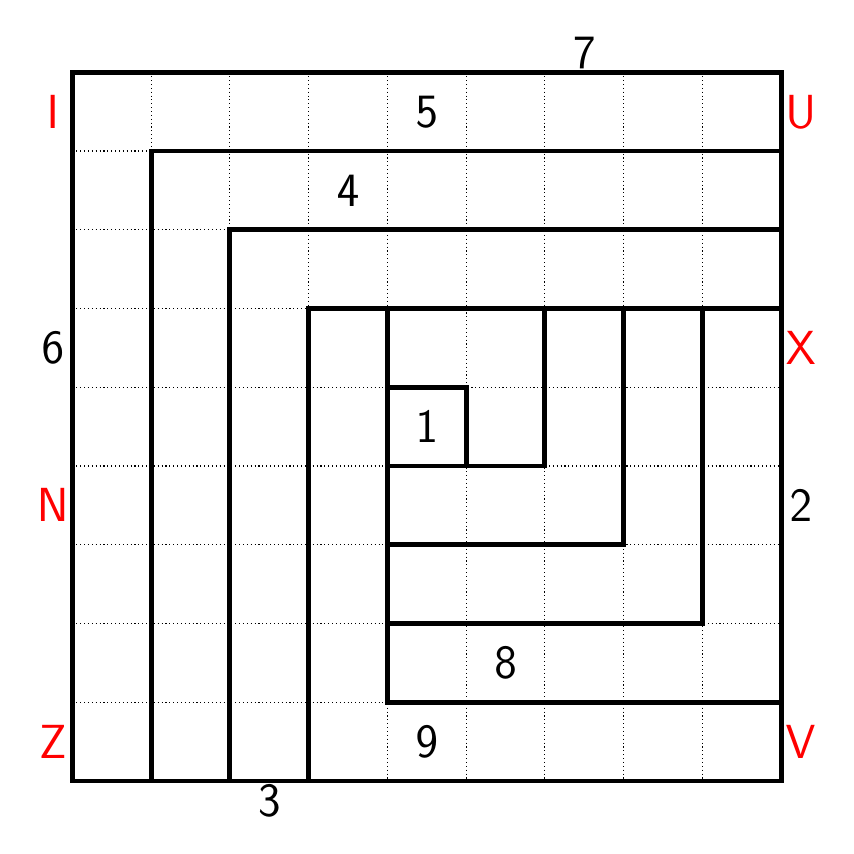
\begin{tikzpicture}
\drawthick (0,8)--++(0,1)--++(9,0)--++(0,-1)--++(-8,0)--++(0,-8)--++(-1,0)--cycle;
    \drawthick (1,7)--++(0,1)--++(8,0)--++(0,-1)--++(-7,0)--++(0,-7)--++(-1,0)--cycle;
    \drawthick (2,6)--++(0,1)--++(7,0)--++(0,-1)--++(-6,0)--++(0,-6)--++(-1,0)--cycle;
    \drawthick (3,0)--++(0,6)--++(1,0)--++(0,-5)--++(5,0)--++(0,-1)--cycle;
    \drawthick (8,1)--++(-4,0)--++(0,1)--++(4,0)--++(0,4)--++(1,0)--++(0,-5)--cycle;
    \drawthick (7,2)--++(-3,0)--++(0,1)--++(3,0)--++(0,3)--++(1,0)--++(0,-4)--cycle;
    \drawthick (6,3)--++(-2,0)--++(0,1)--++(2,0)--++(0,2)--++(1,0)--++(0,-3)--cycle;
    \drawthick (5,5)--++(-1,0)--++(0,1)--++(2,0)--++(0,-2)--++(-1,0)--cycle;\drawgriddotted{9}
\numbersquare{1}{5}{5}\numbersquare{9}{5}{1}\numbersquare{8}{6}{2}\numbersquare{4}{4}{8}\numbersquare{5}{5}{9}\numbersquare{3}{3.0}{0.25}\numbersquare{2}{9.75}{4.0}\numbersquare{6}{0.25}{6.0}\numbersquare{7}{7.0}{9.75}\numbersquare{\textcolor{red}{I}}{0.25}{9.0}\numbersquare{\textcolor{red}{N}}{0.25}{4.0}\numbersquare{\textcolor{red}{Z}}{0.25}{1.0}\numbersquare{\textcolor{red}{V}}{9.75}{1.0}\numbersquare{\textcolor{red}{X}}{9.75}{6.0}\numbersquare{\textcolor{red}{U}}{9.75}{9.0}\end{tikzpicture}}
\vspace{1pc}\noindent{\large \texttt{\string{1:1, 2:3, 3:7, 4:8, 5:9, 6:4, 7:[], 8:5, 9:6\string}}}

\medskip\noindent{\large \texttt{digit(s) 7 cannot be assigned to any hook}}

\clearpage\resizebox{29.5pc}{!}{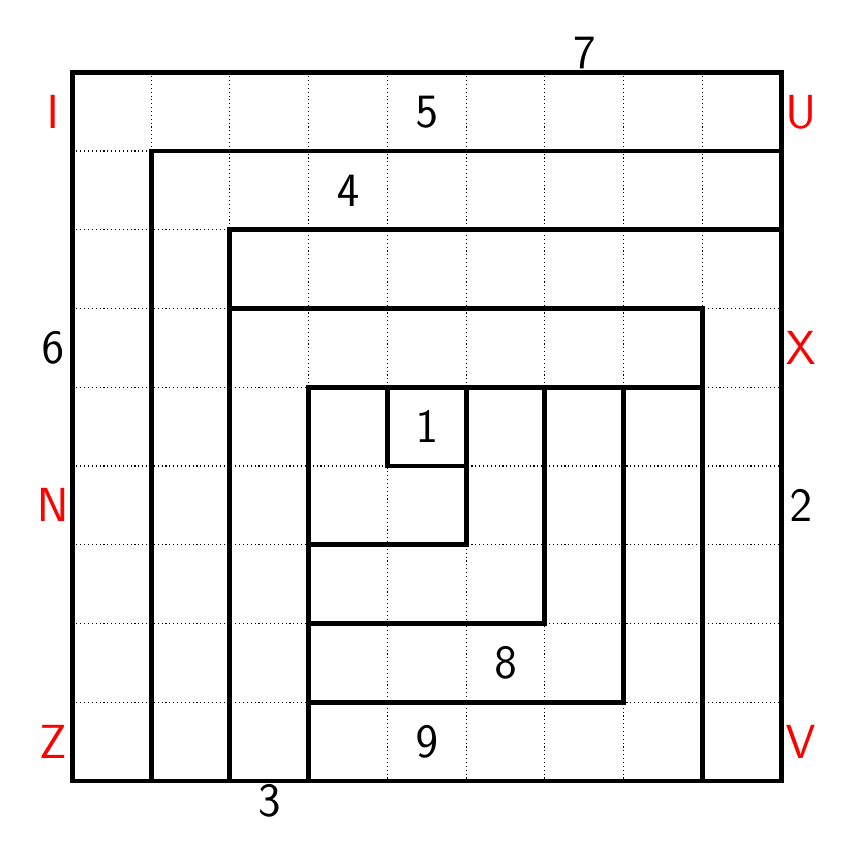
\begin{tikzpicture}
\drawthick (0,8)--++(0,1)--++(9,0)--++(0,-1)--++(-8,0)--++(0,-8)--++(-1,0)--cycle;
    \drawthick (1,7)--++(0,1)--++(8,0)--++(0,-1)--++(-7,0)--++(0,-7)--++(-1,0)--cycle;
    \drawthick (8,6)--++(-6,0)--++(0,1)--++(7,0)--++(0,-7)--++(-1,0)--cycle;
    \drawthick (2,5)--++(0,1)--++(6,0)--++(0,-1)--++(-5,0)--++(0,-5)--++(-1,0)--cycle;
    \drawthick (7,0)--++(-4,0)--++(0,1)--++(4,0)--++(0,4)--++(1,0)--++(0,-5)--cycle;
    \drawthick (6,1)--++(-3,0)--++(0,1)--++(3,0)--++(0,3)--++(1,0)--++(0,-4)--cycle;
    \drawthick (5,2)--++(-2,0)--++(0,1)--++(2,0)--++(0,2)--++(1,0)--++(0,-3)--cycle;
    \drawthick (3,3)--++(0,2)--++(1,0)--++(0,-1)--++(1,0)--++(0,-1)--cycle;\drawgriddotted{9}
\numbersquare{1}{5}{5}\numbersquare{9}{5}{1}\numbersquare{8}{6}{2}\numbersquare{4}{4}{8}\numbersquare{5}{5}{9}\numbersquare{3}{3.0}{0.25}\numbersquare{2}{9.75}{4.0}\numbersquare{6}{0.25}{6.0}\numbersquare{7}{7.0}{9.75}\numbersquare{\textcolor{red}{I}}{0.25}{9.0}\numbersquare{\textcolor{red}{N}}{0.25}{4.0}\numbersquare{\textcolor{red}{Z}}{0.25}{1.0}\numbersquare{\textcolor{red}{V}}{9.75}{1.0}\numbersquare{\textcolor{red}{X}}{9.75}{6.0}\numbersquare{\textcolor{red}{U}}{9.75}{9.0}\end{tikzpicture}}
\vspace{1pc}\noindent{\large \texttt{\string{1:1, 2:$\sqcup$, 3:$\sqcup$, 4:$\sqcup$, 5:$\sqcup$, 6:$\sqcup$, 7:$\sqcup$, 8:$\sqcup$, 9:5\string}}}

\medskip\noindent{\large \texttt{hook 4 is too small for digit 8}}

\clearpage\resizebox{29.5pc}{!}{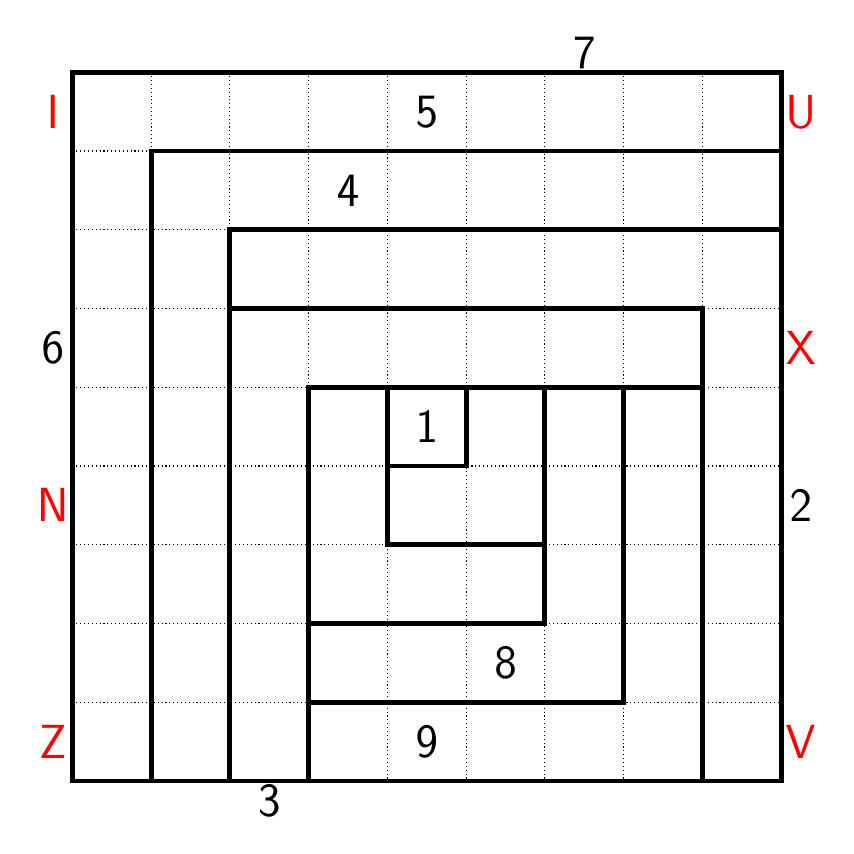
\begin{tikzpicture}
\drawthick (0,8)--++(0,1)--++(9,0)--++(0,-1)--++(-8,0)--++(0,-8)--++(-1,0)--cycle;
    \drawthick (1,7)--++(0,1)--++(8,0)--++(0,-1)--++(-7,0)--++(0,-7)--++(-1,0)--cycle;
    \drawthick (8,6)--++(-6,0)--++(0,1)--++(7,0)--++(0,-7)--++(-1,0)--cycle;
    \drawthick (2,5)--++(0,1)--++(6,0)--++(0,-1)--++(-5,0)--++(0,-5)--++(-1,0)--cycle;
    \drawthick (7,0)--++(-4,0)--++(0,1)--++(4,0)--++(0,4)--++(1,0)--++(0,-5)--cycle;
    \drawthick (6,1)--++(-3,0)--++(0,1)--++(3,0)--++(0,3)--++(1,0)--++(0,-4)--cycle;
    \drawthick (3,2)--++(0,3)--++(1,0)--++(0,-2)--++(2,0)--++(0,-1)--cycle;
    \drawthick (5,3)--++(-1,0)--++(0,1)--++(1,0)--++(0,1)--++(1,0)--++(0,-2)--cycle;\drawgriddotted{9}
\numbersquare{1}{5}{5}\numbersquare{9}{5}{1}\numbersquare{8}{6}{2}\numbersquare{4}{4}{8}\numbersquare{5}{5}{9}\numbersquare{3}{3.0}{0.25}\numbersquare{2}{9.75}{4.0}\numbersquare{6}{0.25}{6.0}\numbersquare{7}{7.0}{9.75}\numbersquare{\textcolor{red}{I}}{0.25}{9.0}\numbersquare{\textcolor{red}{N}}{0.25}{4.0}\numbersquare{\textcolor{red}{Z}}{0.25}{1.0}\numbersquare{\textcolor{red}{V}}{9.75}{1.0}\numbersquare{\textcolor{red}{X}}{9.75}{6.0}\numbersquare{\textcolor{red}{U}}{9.75}{9.0}\end{tikzpicture}}
\vspace{1pc}\noindent{\large \texttt{\string{1:1, 2:$\sqcup$, 3:$\sqcup$, 4:$\sqcup$, 5:$\sqcup$, 6:$\sqcup$, 7:$\sqcup$, 8:$\sqcup$, 9:5\string}}}

\medskip\noindent{\large \texttt{hook 4 is too small for digit 8}}

\clearpage\resizebox{29.5pc}{!}{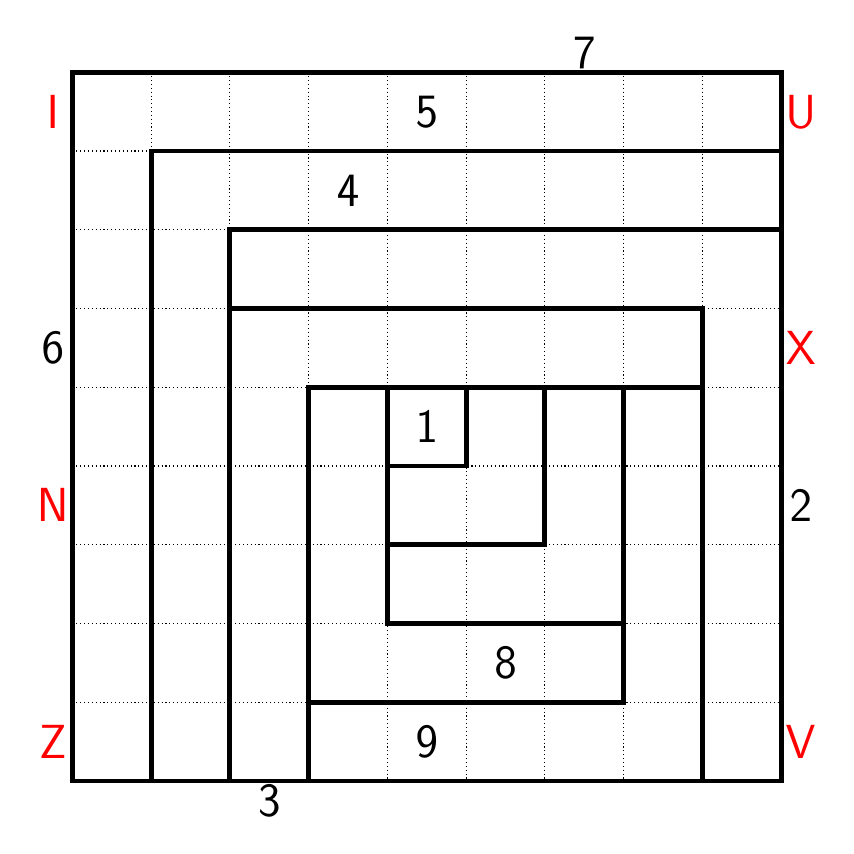
\begin{tikzpicture}
\drawthick (0,8)--++(0,1)--++(9,0)--++(0,-1)--++(-8,0)--++(0,-8)--++(-1,0)--cycle;
    \drawthick (1,7)--++(0,1)--++(8,0)--++(0,-1)--++(-7,0)--++(0,-7)--++(-1,0)--cycle;
    \drawthick (8,6)--++(-6,0)--++(0,1)--++(7,0)--++(0,-7)--++(-1,0)--cycle;
    \drawthick (2,5)--++(0,1)--++(6,0)--++(0,-1)--++(-5,0)--++(0,-5)--++(-1,0)--cycle;
    \drawthick (7,0)--++(-4,0)--++(0,1)--++(4,0)--++(0,4)--++(1,0)--++(0,-5)--cycle;
    \drawthick (3,1)--++(0,4)--++(1,0)--++(0,-3)--++(3,0)--++(0,-1)--cycle;
    \drawthick (6,2)--++(-2,0)--++(0,1)--++(2,0)--++(0,2)--++(1,0)--++(0,-3)--cycle;
    \drawthick (5,3)--++(-1,0)--++(0,1)--++(1,0)--++(0,1)--++(1,0)--++(0,-2)--cycle;\drawgriddotted{9}
\numbersquare{1}{5}{5}\numbersquare{9}{5}{1}\numbersquare{8}{6}{2}\numbersquare{4}{4}{8}\numbersquare{5}{5}{9}\numbersquare{3}{3.0}{0.25}\numbersquare{2}{9.75}{4.0}\numbersquare{6}{0.25}{6.0}\numbersquare{7}{7.0}{9.75}\numbersquare{\textcolor{red}{I}}{0.25}{9.0}\numbersquare{\textcolor{red}{N}}{0.25}{4.0}\numbersquare{\textcolor{red}{Z}}{0.25}{1.0}\numbersquare{\textcolor{red}{V}}{9.75}{1.0}\numbersquare{\textcolor{red}{X}}{9.75}{6.0}\numbersquare{\textcolor{red}{U}}{9.75}{9.0}\end{tikzpicture}}
\vspace{1pc}\noindent{\large \texttt{\string{1:1, 2:$\sqcup$, 3:$\sqcup$, 4:$\sqcup$, 5:$\sqcup$, 6:$\sqcup$, 7:$\sqcup$, 8:$\sqcup$, 9:5\string}}}

\medskip\noindent{\large \texttt{hook 4 is too small for digit 8}}

\clearpage\resizebox{29.5pc}{!}{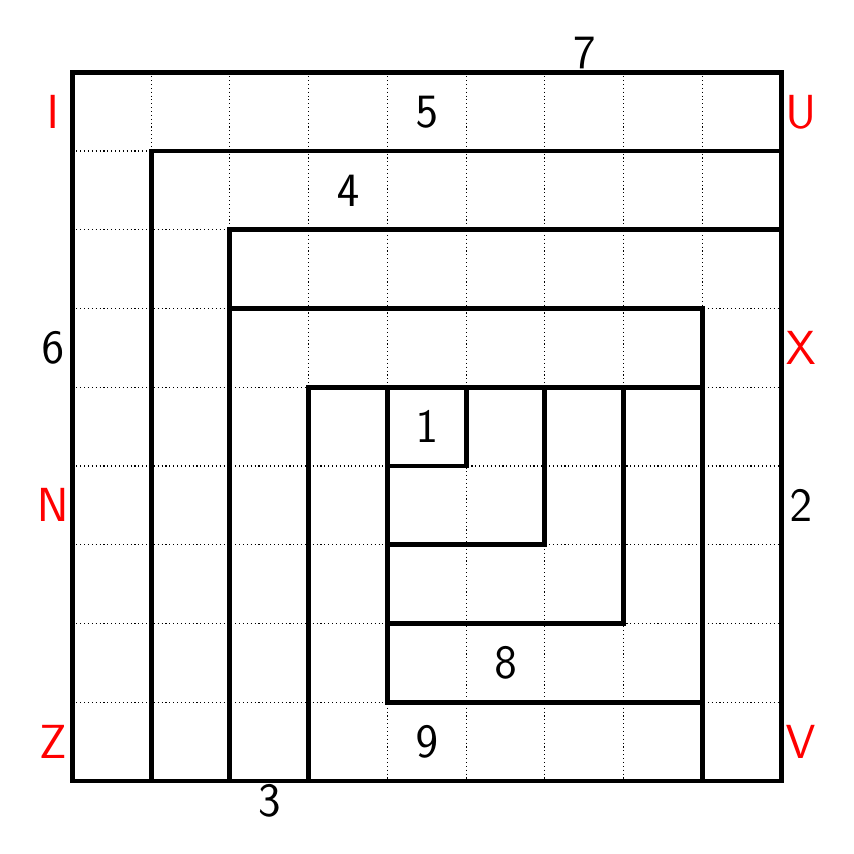
\begin{tikzpicture}
\drawthick (0,8)--++(0,1)--++(9,0)--++(0,-1)--++(-8,0)--++(0,-8)--++(-1,0)--cycle;
    \drawthick (1,7)--++(0,1)--++(8,0)--++(0,-1)--++(-7,0)--++(0,-7)--++(-1,0)--cycle;
    \drawthick (8,6)--++(-6,0)--++(0,1)--++(7,0)--++(0,-7)--++(-1,0)--cycle;
    \drawthick (2,5)--++(0,1)--++(6,0)--++(0,-1)--++(-5,0)--++(0,-5)--++(-1,0)--cycle;
    \drawthick (3,0)--++(0,5)--++(1,0)--++(0,-4)--++(4,0)--++(0,-1)--cycle;
    \drawthick (7,1)--++(-3,0)--++(0,1)--++(3,0)--++(0,3)--++(1,0)--++(0,-4)--cycle;
    \drawthick (6,2)--++(-2,0)--++(0,1)--++(2,0)--++(0,2)--++(1,0)--++(0,-3)--cycle;
    \drawthick (5,3)--++(-1,0)--++(0,1)--++(1,0)--++(0,1)--++(1,0)--++(0,-2)--cycle;\drawgriddotted{9}
\numbersquare{1}{5}{5}\numbersquare{9}{5}{1}\numbersquare{8}{6}{2}\numbersquare{4}{4}{8}\numbersquare{5}{5}{9}\numbersquare{3}{3.0}{0.25}\numbersquare{2}{9.75}{4.0}\numbersquare{6}{0.25}{6.0}\numbersquare{7}{7.0}{9.75}\numbersquare{\textcolor{red}{I}}{0.25}{9.0}\numbersquare{\textcolor{red}{N}}{0.25}{4.0}\numbersquare{\textcolor{red}{Z}}{0.25}{1.0}\numbersquare{\textcolor{red}{V}}{9.75}{1.0}\numbersquare{\textcolor{red}{X}}{9.75}{6.0}\numbersquare{\textcolor{red}{U}}{9.75}{9.0}\end{tikzpicture}}
\vspace{1pc}\noindent{\large \texttt{\string{1:1, 2:$\sqcup$, 3:$\sqcup$, 4:$\sqcup$, 5:$\sqcup$, 6:$\sqcup$, 7:$\sqcup$, 8:$\sqcup$, 9:5\string}}}

\medskip\noindent{\large \texttt{hook 4 is too small for digit 8}}

\clearpage\resizebox{29.5pc}{!}{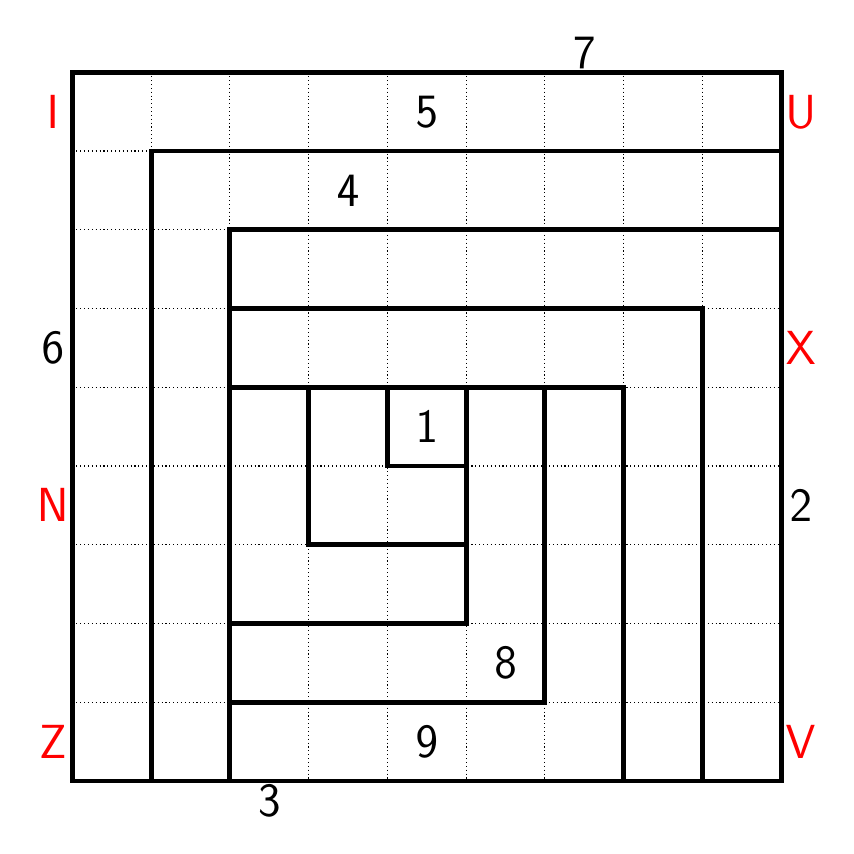
\begin{tikzpicture}
\drawthick (0,8)--++(0,1)--++(9,0)--++(0,-1)--++(-8,0)--++(0,-8)--++(-1,0)--cycle;
    \drawthick (1,7)--++(0,1)--++(8,0)--++(0,-1)--++(-7,0)--++(0,-7)--++(-1,0)--cycle;
    \drawthick (8,6)--++(-6,0)--++(0,1)--++(7,0)--++(0,-7)--++(-1,0)--cycle;
    \drawthick (7,5)--++(-5,0)--++(0,1)--++(6,0)--++(0,-6)--++(-1,0)--cycle;
    \drawthick (6,0)--++(-4,0)--++(0,1)--++(4,0)--++(0,4)--++(1,0)--++(0,-5)--cycle;
    \drawthick (5,1)--++(-3,0)--++(0,1)--++(3,0)--++(0,3)--++(1,0)--++(0,-4)--cycle;
    \drawthick (2,2)--++(0,3)--++(1,0)--++(0,-2)--++(2,0)--++(0,-1)--cycle;
    \drawthick (3,3)--++(0,2)--++(1,0)--++(0,-1)--++(1,0)--++(0,-1)--cycle;\drawgriddotted{9}
\numbersquare{1}{5}{5}\numbersquare{9}{5}{1}\numbersquare{8}{6}{2}\numbersquare{4}{4}{8}\numbersquare{5}{5}{9}\numbersquare{3}{3.0}{0.25}\numbersquare{2}{9.75}{4.0}\numbersquare{6}{0.25}{6.0}\numbersquare{7}{7.0}{9.75}\numbersquare{\textcolor{red}{I}}{0.25}{9.0}\numbersquare{\textcolor{red}{N}}{0.25}{4.0}\numbersquare{\textcolor{red}{Z}}{0.25}{1.0}\numbersquare{\textcolor{red}{V}}{9.75}{1.0}\numbersquare{\textcolor{red}{X}}{9.75}{6.0}\numbersquare{\textcolor{red}{U}}{9.75}{9.0}\end{tikzpicture}}
\vspace{1pc}\noindent{\large \texttt{\string{1:1, 2:$\sqcup$, 3:$\sqcup$, 4:$\sqcup$, 5:$\sqcup$, 6:$\sqcup$, 7:$\sqcup$, 8:$\sqcup$, 9:5\string}}}

\medskip\noindent{\large \texttt{hook 4 is too small for digit 8}}

\clearpage\resizebox{29.5pc}{!}{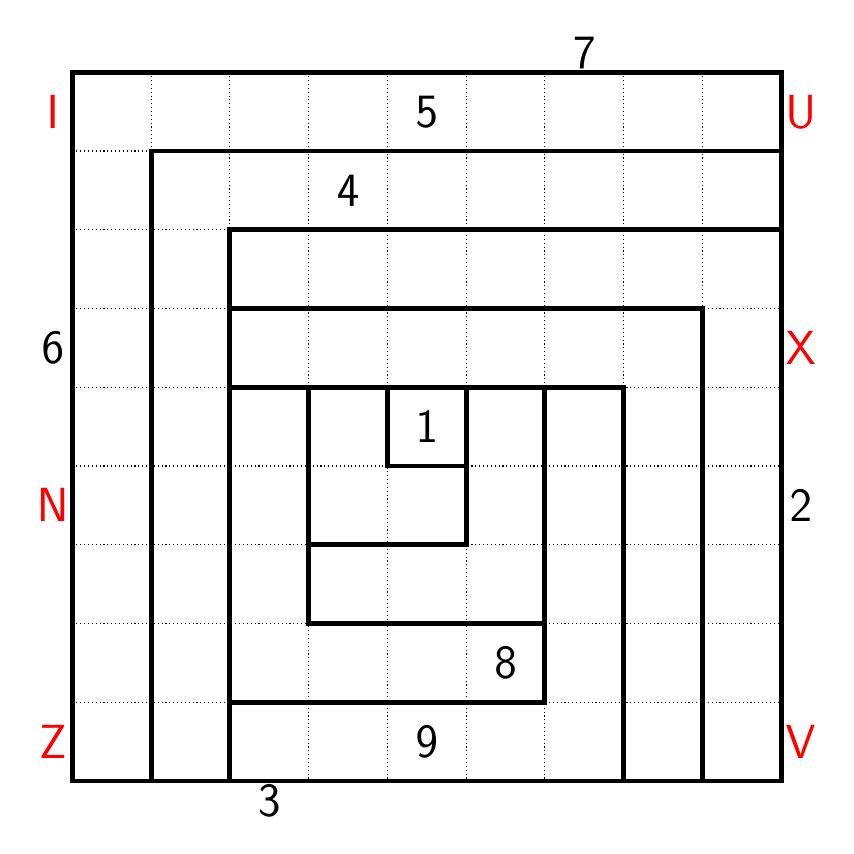
\begin{tikzpicture}
\drawthick (0,8)--++(0,1)--++(9,0)--++(0,-1)--++(-8,0)--++(0,-8)--++(-1,0)--cycle;
    \drawthick (1,7)--++(0,1)--++(8,0)--++(0,-1)--++(-7,0)--++(0,-7)--++(-1,0)--cycle;
    \drawthick (8,6)--++(-6,0)--++(0,1)--++(7,0)--++(0,-7)--++(-1,0)--cycle;
    \drawthick (7,5)--++(-5,0)--++(0,1)--++(6,0)--++(0,-6)--++(-1,0)--cycle;
    \drawthick (6,0)--++(-4,0)--++(0,1)--++(4,0)--++(0,4)--++(1,0)--++(0,-5)--cycle;
    \drawthick (2,1)--++(0,4)--++(1,0)--++(0,-3)--++(3,0)--++(0,-1)--cycle;
    \drawthick (5,2)--++(-2,0)--++(0,1)--++(2,0)--++(0,2)--++(1,0)--++(0,-3)--cycle;
    \drawthick (3,3)--++(0,2)--++(1,0)--++(0,-1)--++(1,0)--++(0,-1)--cycle;\drawgriddotted{9}
\numbersquare{1}{5}{5}\numbersquare{9}{5}{1}\numbersquare{8}{6}{2}\numbersquare{4}{4}{8}\numbersquare{5}{5}{9}\numbersquare{3}{3.0}{0.25}\numbersquare{2}{9.75}{4.0}\numbersquare{6}{0.25}{6.0}\numbersquare{7}{7.0}{9.75}\numbersquare{\textcolor{red}{I}}{0.25}{9.0}\numbersquare{\textcolor{red}{N}}{0.25}{4.0}\numbersquare{\textcolor{red}{Z}}{0.25}{1.0}\numbersquare{\textcolor{red}{V}}{9.75}{1.0}\numbersquare{\textcolor{red}{X}}{9.75}{6.0}\numbersquare{\textcolor{red}{U}}{9.75}{9.0}\end{tikzpicture}}
\vspace{1pc}\noindent{\large \texttt{\string{1:1, 2:$\sqcup$, 3:$\sqcup$, 4:$\sqcup$, 5:$\sqcup$, 6:$\sqcup$, 7:$\sqcup$, 8:$\sqcup$, 9:5\string}}}

\medskip\noindent{\large \texttt{hook 4 is too small for digit 8}}

\clearpage\resizebox{29.5pc}{!}{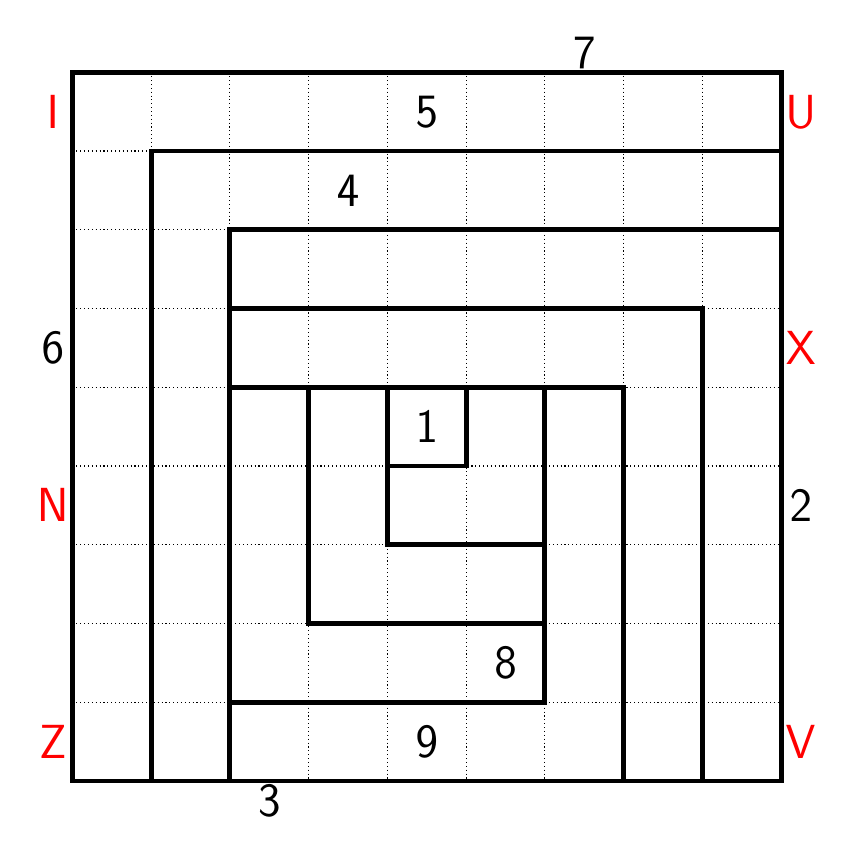
\begin{tikzpicture}
\drawthick (0,8)--++(0,1)--++(9,0)--++(0,-1)--++(-8,0)--++(0,-8)--++(-1,0)--cycle;
    \drawthick (1,7)--++(0,1)--++(8,0)--++(0,-1)--++(-7,0)--++(0,-7)--++(-1,0)--cycle;
    \drawthick (8,6)--++(-6,0)--++(0,1)--++(7,0)--++(0,-7)--++(-1,0)--cycle;
    \drawthick (7,5)--++(-5,0)--++(0,1)--++(6,0)--++(0,-6)--++(-1,0)--cycle;
    \drawthick (6,0)--++(-4,0)--++(0,1)--++(4,0)--++(0,4)--++(1,0)--++(0,-5)--cycle;
    \drawthick (2,1)--++(0,4)--++(1,0)--++(0,-3)--++(3,0)--++(0,-1)--cycle;
    \drawthick (3,2)--++(0,3)--++(1,0)--++(0,-2)--++(2,0)--++(0,-1)--cycle;
    \drawthick (5,3)--++(-1,0)--++(0,1)--++(1,0)--++(0,1)--++(1,0)--++(0,-2)--cycle;\drawgriddotted{9}
\numbersquare{1}{5}{5}\numbersquare{9}{5}{1}\numbersquare{8}{6}{2}\numbersquare{4}{4}{8}\numbersquare{5}{5}{9}\numbersquare{3}{3.0}{0.25}\numbersquare{2}{9.75}{4.0}\numbersquare{6}{0.25}{6.0}\numbersquare{7}{7.0}{9.75}\numbersquare{\textcolor{red}{I}}{0.25}{9.0}\numbersquare{\textcolor{red}{N}}{0.25}{4.0}\numbersquare{\textcolor{red}{Z}}{0.25}{1.0}\numbersquare{\textcolor{red}{V}}{9.75}{1.0}\numbersquare{\textcolor{red}{X}}{9.75}{6.0}\numbersquare{\textcolor{red}{U}}{9.75}{9.0}\end{tikzpicture}}
\vspace{1pc}\noindent{\large \texttt{\string{1:1, 2:$\sqcup$, 3:$\sqcup$, 4:$\sqcup$, 5:$\sqcup$, 6:$\sqcup$, 7:$\sqcup$, 8:$\sqcup$, 9:5\string}}}

\medskip\noindent{\large \texttt{hook 4 is too small for digit 8}}

\clearpage\resizebox{29.5pc}{!}{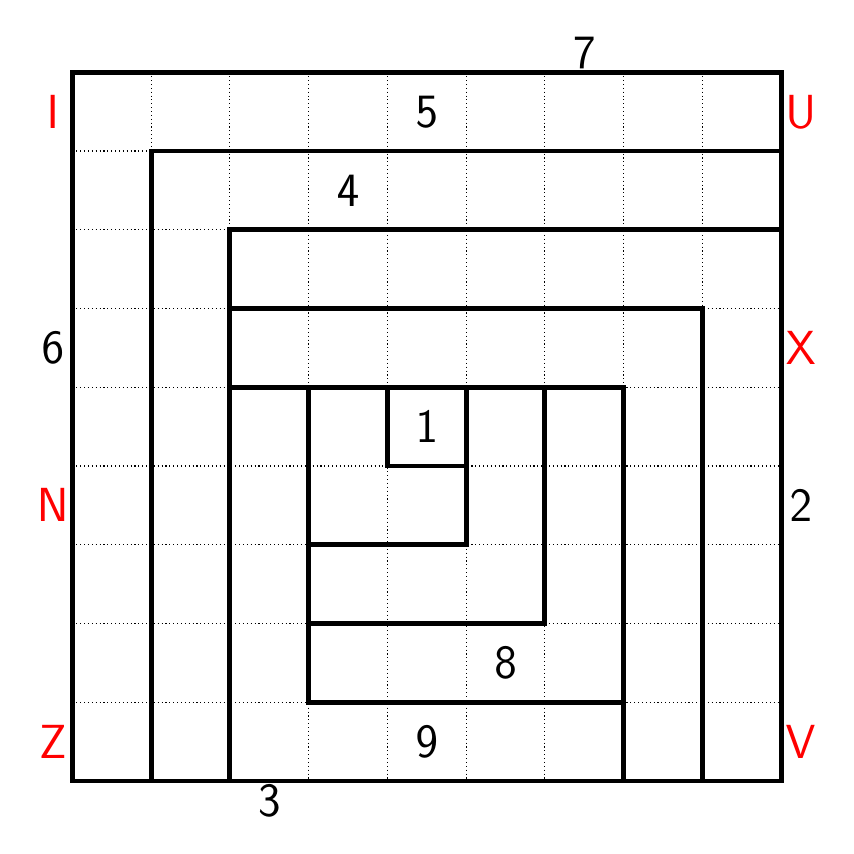
\begin{tikzpicture}
\drawthick (0,8)--++(0,1)--++(9,0)--++(0,-1)--++(-8,0)--++(0,-8)--++(-1,0)--cycle;
    \drawthick (1,7)--++(0,1)--++(8,0)--++(0,-1)--++(-7,0)--++(0,-7)--++(-1,0)--cycle;
    \drawthick (8,6)--++(-6,0)--++(0,1)--++(7,0)--++(0,-7)--++(-1,0)--cycle;
    \drawthick (7,5)--++(-5,0)--++(0,1)--++(6,0)--++(0,-6)--++(-1,0)--cycle;
    \drawthick (2,0)--++(0,5)--++(1,0)--++(0,-4)--++(4,0)--++(0,-1)--cycle;
    \drawthick (6,1)--++(-3,0)--++(0,1)--++(3,0)--++(0,3)--++(1,0)--++(0,-4)--cycle;
    \drawthick (5,2)--++(-2,0)--++(0,1)--++(2,0)--++(0,2)--++(1,0)--++(0,-3)--cycle;
    \drawthick (3,3)--++(0,2)--++(1,0)--++(0,-1)--++(1,0)--++(0,-1)--cycle;\drawgriddotted{9}
\numbersquare{1}{5}{5}\numbersquare{9}{5}{1}\numbersquare{8}{6}{2}\numbersquare{4}{4}{8}\numbersquare{5}{5}{9}\numbersquare{3}{3.0}{0.25}\numbersquare{2}{9.75}{4.0}\numbersquare{6}{0.25}{6.0}\numbersquare{7}{7.0}{9.75}\numbersquare{\textcolor{red}{I}}{0.25}{9.0}\numbersquare{\textcolor{red}{N}}{0.25}{4.0}\numbersquare{\textcolor{red}{Z}}{0.25}{1.0}\numbersquare{\textcolor{red}{V}}{9.75}{1.0}\numbersquare{\textcolor{red}{X}}{9.75}{6.0}\numbersquare{\textcolor{red}{U}}{9.75}{9.0}\end{tikzpicture}}
\vspace{1pc}\noindent{\large \texttt{\string{1:1, 2:$\sqcup$, 3:$\sqcup$, 4:$\sqcup$, 5:$\sqcup$, 6:$\sqcup$, 7:$\sqcup$, 8:$\sqcup$, 9:5\string}}}

\medskip\noindent{\large \texttt{hook 4 is too small for digit 8}}

\clearpage\resizebox{29.5pc}{!}{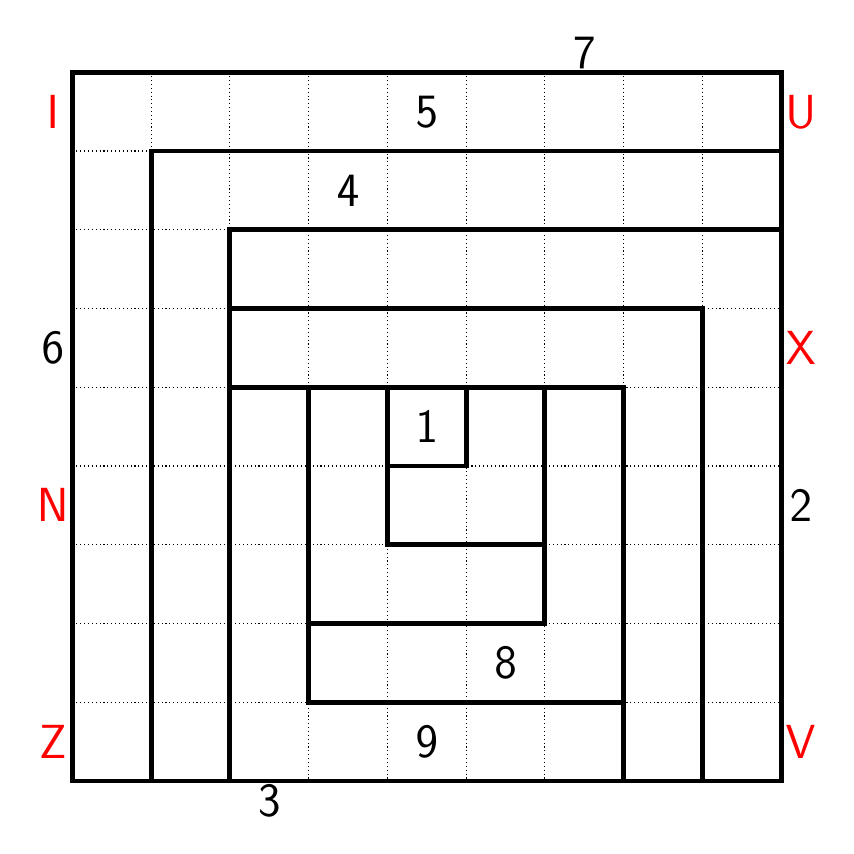
\begin{tikzpicture}
\drawthick (0,8)--++(0,1)--++(9,0)--++(0,-1)--++(-8,0)--++(0,-8)--++(-1,0)--cycle;
    \drawthick (1,7)--++(0,1)--++(8,0)--++(0,-1)--++(-7,0)--++(0,-7)--++(-1,0)--cycle;
    \drawthick (8,6)--++(-6,0)--++(0,1)--++(7,0)--++(0,-7)--++(-1,0)--cycle;
    \drawthick (7,5)--++(-5,0)--++(0,1)--++(6,0)--++(0,-6)--++(-1,0)--cycle;
    \drawthick (2,0)--++(0,5)--++(1,0)--++(0,-4)--++(4,0)--++(0,-1)--cycle;
    \drawthick (6,1)--++(-3,0)--++(0,1)--++(3,0)--++(0,3)--++(1,0)--++(0,-4)--cycle;
    \drawthick (3,2)--++(0,3)--++(1,0)--++(0,-2)--++(2,0)--++(0,-1)--cycle;
    \drawthick (5,3)--++(-1,0)--++(0,1)--++(1,0)--++(0,1)--++(1,0)--++(0,-2)--cycle;\drawgriddotted{9}
\numbersquare{1}{5}{5}\numbersquare{9}{5}{1}\numbersquare{8}{6}{2}\numbersquare{4}{4}{8}\numbersquare{5}{5}{9}\numbersquare{3}{3.0}{0.25}\numbersquare{2}{9.75}{4.0}\numbersquare{6}{0.25}{6.0}\numbersquare{7}{7.0}{9.75}\numbersquare{\textcolor{red}{I}}{0.25}{9.0}\numbersquare{\textcolor{red}{N}}{0.25}{4.0}\numbersquare{\textcolor{red}{Z}}{0.25}{1.0}\numbersquare{\textcolor{red}{V}}{9.75}{1.0}\numbersquare{\textcolor{red}{X}}{9.75}{6.0}\numbersquare{\textcolor{red}{U}}{9.75}{9.0}\end{tikzpicture}}
\vspace{1pc}\noindent{\large \texttt{\string{1:1, 2:$\sqcup$, 3:$\sqcup$, 4:$\sqcup$, 5:$\sqcup$, 6:$\sqcup$, 7:$\sqcup$, 8:$\sqcup$, 9:5\string}}}

\medskip\noindent{\large \texttt{hook 4 is too small for digit 8}}

\clearpage\resizebox{29.5pc}{!}{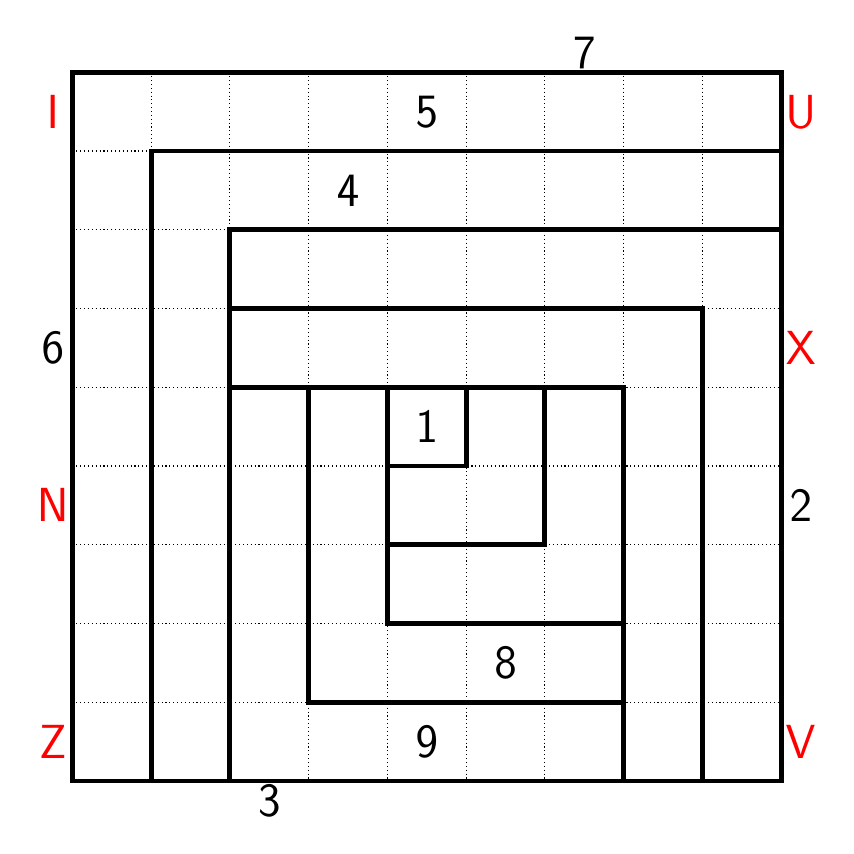
\begin{tikzpicture}
\drawthick (0,8)--++(0,1)--++(9,0)--++(0,-1)--++(-8,0)--++(0,-8)--++(-1,0)--cycle;
    \drawthick (1,7)--++(0,1)--++(8,0)--++(0,-1)--++(-7,0)--++(0,-7)--++(-1,0)--cycle;
    \drawthick (8,6)--++(-6,0)--++(0,1)--++(7,0)--++(0,-7)--++(-1,0)--cycle;
    \drawthick (7,5)--++(-5,0)--++(0,1)--++(6,0)--++(0,-6)--++(-1,0)--cycle;
    \drawthick (2,0)--++(0,5)--++(1,0)--++(0,-4)--++(4,0)--++(0,-1)--cycle;
    \drawthick (3,1)--++(0,4)--++(1,0)--++(0,-3)--++(3,0)--++(0,-1)--cycle;
    \drawthick (6,2)--++(-2,0)--++(0,1)--++(2,0)--++(0,2)--++(1,0)--++(0,-3)--cycle;
    \drawthick (5,3)--++(-1,0)--++(0,1)--++(1,0)--++(0,1)--++(1,0)--++(0,-2)--cycle;\drawgriddotted{9}
\numbersquare{1}{5}{5}\numbersquare{9}{5}{1}\numbersquare{8}{6}{2}\numbersquare{4}{4}{8}\numbersquare{5}{5}{9}\numbersquare{3}{3.0}{0.25}\numbersquare{2}{9.75}{4.0}\numbersquare{6}{0.25}{6.0}\numbersquare{7}{7.0}{9.75}\numbersquare{\textcolor{red}{I}}{0.25}{9.0}\numbersquare{\textcolor{red}{N}}{0.25}{4.0}\numbersquare{\textcolor{red}{Z}}{0.25}{1.0}\numbersquare{\textcolor{red}{V}}{9.75}{1.0}\numbersquare{\textcolor{red}{X}}{9.75}{6.0}\numbersquare{\textcolor{red}{U}}{9.75}{9.0}\end{tikzpicture}}
\vspace{1pc}\noindent{\large \texttt{\string{1:1, 2:$\sqcup$, 3:$\sqcup$, 4:$\sqcup$, 5:$\sqcup$, 6:$\sqcup$, 7:$\sqcup$, 8:$\sqcup$, 9:5\string}}}

\medskip\noindent{\large \texttt{hook 4 is too small for digit 8}}

\clearpage\resizebox{29.5pc}{!}{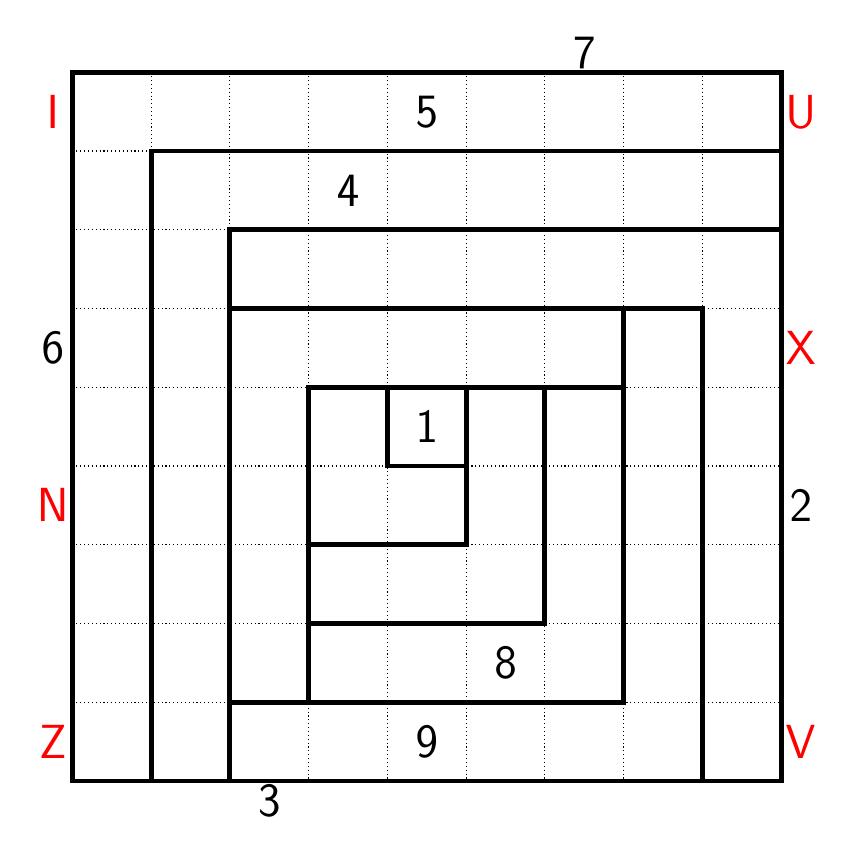
\begin{tikzpicture}
\drawthick (0,8)--++(0,1)--++(9,0)--++(0,-1)--++(-8,0)--++(0,-8)--++(-1,0)--cycle;
    \drawthick (1,7)--++(0,1)--++(8,0)--++(0,-1)--++(-7,0)--++(0,-7)--++(-1,0)--cycle;
    \drawthick (8,6)--++(-6,0)--++(0,1)--++(7,0)--++(0,-7)--++(-1,0)--cycle;
    \drawthick (7,0)--++(-5,0)--++(0,1)--++(5,0)--++(0,5)--++(1,0)--++(0,-6)--cycle;
    \drawthick (2,5)--++(0,1)--++(5,0)--++(0,-1)--++(-4,0)--++(0,-4)--++(-1,0)--cycle;
    \drawthick (6,1)--++(-3,0)--++(0,1)--++(3,0)--++(0,3)--++(1,0)--++(0,-4)--cycle;
    \drawthick (5,2)--++(-2,0)--++(0,1)--++(2,0)--++(0,2)--++(1,0)--++(0,-3)--cycle;
    \drawthick (3,3)--++(0,2)--++(1,0)--++(0,-1)--++(1,0)--++(0,-1)--cycle;\drawgriddotted{9}
\numbersquare{1}{5}{5}\numbersquare{9}{5}{1}\numbersquare{8}{6}{2}\numbersquare{4}{4}{8}\numbersquare{5}{5}{9}\numbersquare{3}{3.0}{0.25}\numbersquare{2}{9.75}{4.0}\numbersquare{6}{0.25}{6.0}\numbersquare{7}{7.0}{9.75}\numbersquare{\textcolor{red}{I}}{0.25}{9.0}\numbersquare{\textcolor{red}{N}}{0.25}{4.0}\numbersquare{\textcolor{red}{Z}}{0.25}{1.0}\numbersquare{\textcolor{red}{V}}{9.75}{1.0}\numbersquare{\textcolor{red}{X}}{9.75}{6.0}\numbersquare{\textcolor{red}{U}}{9.75}{9.0}\end{tikzpicture}}
\vspace{1pc}\noindent{\large \texttt{\string{1:1, 2:$\sqcup$, 3:$\sqcup$, 4:$\sqcup$, 5:$\sqcup$, 6:$\sqcup$, 7:$\sqcup$, 8:$\sqcup$, 9:6\string}}}

\medskip\noindent{\large \texttt{hook 4 is too small for digit 8}}

\clearpage\resizebox{29.5pc}{!}{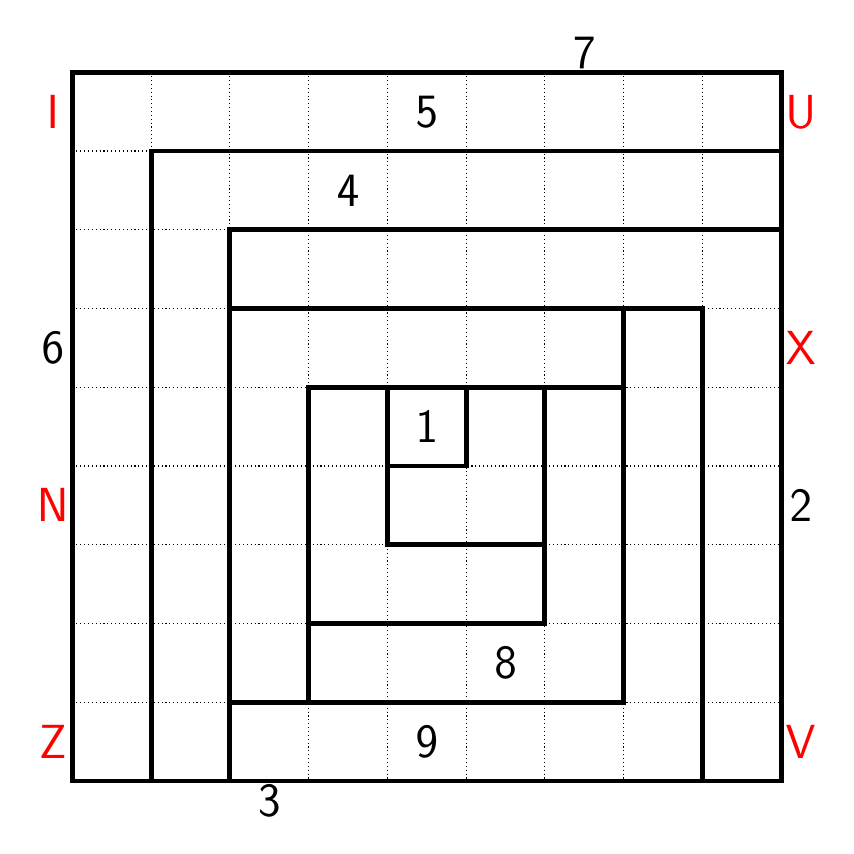
\begin{tikzpicture}
\drawthick (0,8)--++(0,1)--++(9,0)--++(0,-1)--++(-8,0)--++(0,-8)--++(-1,0)--cycle;
    \drawthick (1,7)--++(0,1)--++(8,0)--++(0,-1)--++(-7,0)--++(0,-7)--++(-1,0)--cycle;
    \drawthick (8,6)--++(-6,0)--++(0,1)--++(7,0)--++(0,-7)--++(-1,0)--cycle;
    \drawthick (7,0)--++(-5,0)--++(0,1)--++(5,0)--++(0,5)--++(1,0)--++(0,-6)--cycle;
    \drawthick (2,5)--++(0,1)--++(5,0)--++(0,-1)--++(-4,0)--++(0,-4)--++(-1,0)--cycle;
    \drawthick (6,1)--++(-3,0)--++(0,1)--++(3,0)--++(0,3)--++(1,0)--++(0,-4)--cycle;
    \drawthick (3,2)--++(0,3)--++(1,0)--++(0,-2)--++(2,0)--++(0,-1)--cycle;
    \drawthick (5,3)--++(-1,0)--++(0,1)--++(1,0)--++(0,1)--++(1,0)--++(0,-2)--cycle;\drawgriddotted{9}
\numbersquare{1}{5}{5}\numbersquare{9}{5}{1}\numbersquare{8}{6}{2}\numbersquare{4}{4}{8}\numbersquare{5}{5}{9}\numbersquare{3}{3.0}{0.25}\numbersquare{2}{9.75}{4.0}\numbersquare{6}{0.25}{6.0}\numbersquare{7}{7.0}{9.75}\numbersquare{\textcolor{red}{I}}{0.25}{9.0}\numbersquare{\textcolor{red}{N}}{0.25}{4.0}\numbersquare{\textcolor{red}{Z}}{0.25}{1.0}\numbersquare{\textcolor{red}{V}}{9.75}{1.0}\numbersquare{\textcolor{red}{X}}{9.75}{6.0}\numbersquare{\textcolor{red}{U}}{9.75}{9.0}\end{tikzpicture}}
\vspace{1pc}\noindent{\large \texttt{\string{1:1, 2:$\sqcup$, 3:$\sqcup$, 4:$\sqcup$, 5:$\sqcup$, 6:$\sqcup$, 7:$\sqcup$, 8:$\sqcup$, 9:6\string}}}

\medskip\noindent{\large \texttt{hook 4 is too small for digit 8}}

\clearpage\resizebox{29.5pc}{!}{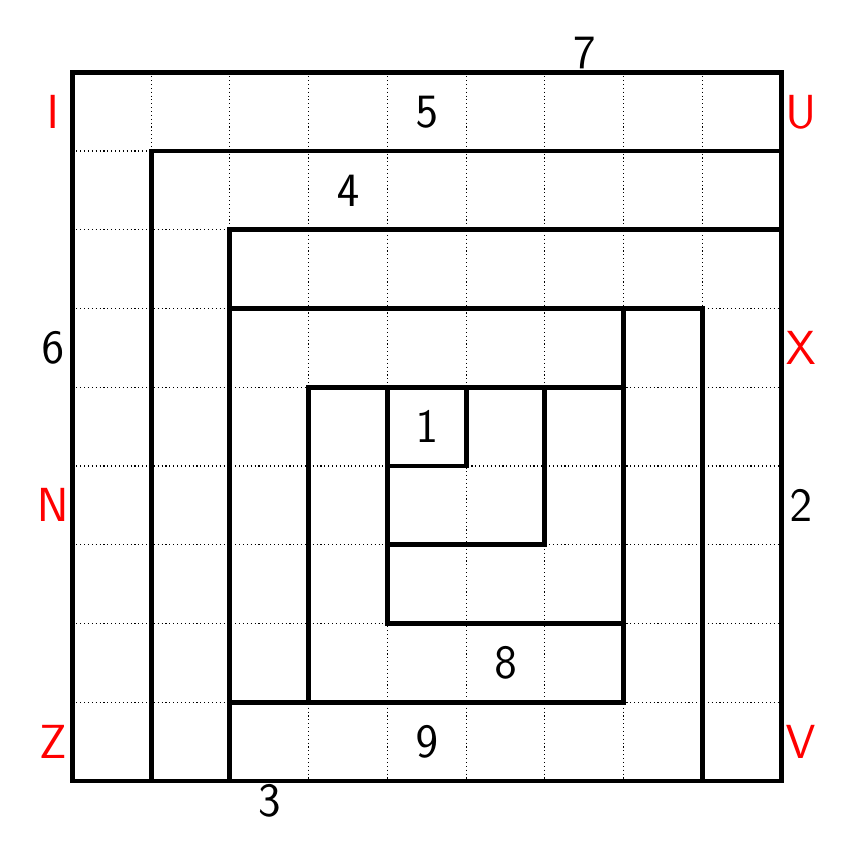
\begin{tikzpicture}
\drawthick (0,8)--++(0,1)--++(9,0)--++(0,-1)--++(-8,0)--++(0,-8)--++(-1,0)--cycle;
    \drawthick (1,7)--++(0,1)--++(8,0)--++(0,-1)--++(-7,0)--++(0,-7)--++(-1,0)--cycle;
    \drawthick (8,6)--++(-6,0)--++(0,1)--++(7,0)--++(0,-7)--++(-1,0)--cycle;
    \drawthick (7,0)--++(-5,0)--++(0,1)--++(5,0)--++(0,5)--++(1,0)--++(0,-6)--cycle;
    \drawthick (2,5)--++(0,1)--++(5,0)--++(0,-1)--++(-4,0)--++(0,-4)--++(-1,0)--cycle;
    \drawthick (3,1)--++(0,4)--++(1,0)--++(0,-3)--++(3,0)--++(0,-1)--cycle;
    \drawthick (6,2)--++(-2,0)--++(0,1)--++(2,0)--++(0,2)--++(1,0)--++(0,-3)--cycle;
    \drawthick (5,3)--++(-1,0)--++(0,1)--++(1,0)--++(0,1)--++(1,0)--++(0,-2)--cycle;\drawgriddotted{9}
\numbersquare{1}{5}{5}\numbersquare{9}{5}{1}\numbersquare{8}{6}{2}\numbersquare{4}{4}{8}\numbersquare{5}{5}{9}\numbersquare{3}{3.0}{0.25}\numbersquare{2}{9.75}{4.0}\numbersquare{6}{0.25}{6.0}\numbersquare{7}{7.0}{9.75}\numbersquare{\textcolor{red}{I}}{0.25}{9.0}\numbersquare{\textcolor{red}{N}}{0.25}{4.0}\numbersquare{\textcolor{red}{Z}}{0.25}{1.0}\numbersquare{\textcolor{red}{V}}{9.75}{1.0}\numbersquare{\textcolor{red}{X}}{9.75}{6.0}\numbersquare{\textcolor{red}{U}}{9.75}{9.0}\end{tikzpicture}}
\vspace{1pc}\noindent{\large \texttt{\string{1:1, 2:$\sqcup$, 3:$\sqcup$, 4:$\sqcup$, 5:$\sqcup$, 6:$\sqcup$, 7:$\sqcup$, 8:$\sqcup$, 9:6\string}}}

\medskip\noindent{\large \texttt{hook 4 is too small for digit 8}}

\clearpage\resizebox{29.5pc}{!}{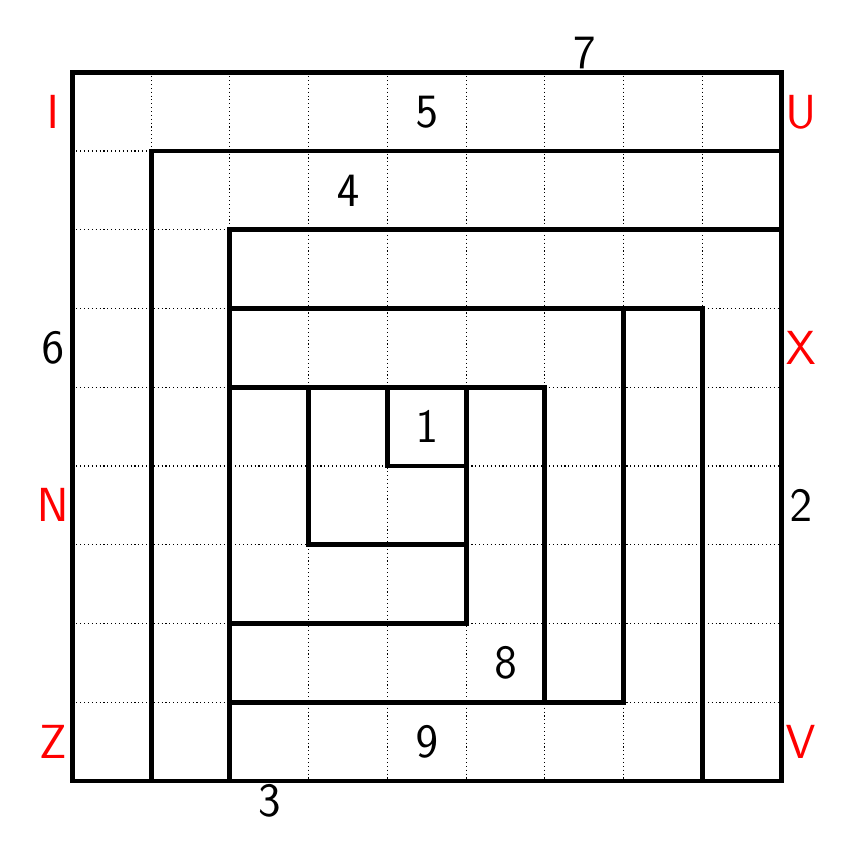
\begin{tikzpicture}
\drawthick (0,8)--++(0,1)--++(9,0)--++(0,-1)--++(-8,0)--++(0,-8)--++(-1,0)--cycle;
    \drawthick (1,7)--++(0,1)--++(8,0)--++(0,-1)--++(-7,0)--++(0,-7)--++(-1,0)--cycle;
    \drawthick (8,6)--++(-6,0)--++(0,1)--++(7,0)--++(0,-7)--++(-1,0)--cycle;
    \drawthick (7,0)--++(-5,0)--++(0,1)--++(5,0)--++(0,5)--++(1,0)--++(0,-6)--cycle;
    \drawthick (6,5)--++(-4,0)--++(0,1)--++(5,0)--++(0,-5)--++(-1,0)--cycle;
    \drawthick (5,1)--++(-3,0)--++(0,1)--++(3,0)--++(0,3)--++(1,0)--++(0,-4)--cycle;
    \drawthick (2,2)--++(0,3)--++(1,0)--++(0,-2)--++(2,0)--++(0,-1)--cycle;
    \drawthick (3,3)--++(0,2)--++(1,0)--++(0,-1)--++(1,0)--++(0,-1)--cycle;\drawgriddotted{9}
\numbersquare{1}{5}{5}\numbersquare{9}{5}{1}\numbersquare{8}{6}{2}\numbersquare{4}{4}{8}\numbersquare{5}{5}{9}\numbersquare{3}{3.0}{0.25}\numbersquare{2}{9.75}{4.0}\numbersquare{6}{0.25}{6.0}\numbersquare{7}{7.0}{9.75}\numbersquare{\textcolor{red}{I}}{0.25}{9.0}\numbersquare{\textcolor{red}{N}}{0.25}{4.0}\numbersquare{\textcolor{red}{Z}}{0.25}{1.0}\numbersquare{\textcolor{red}{V}}{9.75}{1.0}\numbersquare{\textcolor{red}{X}}{9.75}{6.0}\numbersquare{\textcolor{red}{U}}{9.75}{9.0}\end{tikzpicture}}
\vspace{1pc}\noindent{\large \texttt{\string{1:1, 2:$\sqcup$, 3:$\sqcup$, 4:$\sqcup$, 5:$\sqcup$, 6:$\sqcup$, 7:$\sqcup$, 8:$\sqcup$, 9:6\string}}}

\medskip\noindent{\large \texttt{hook 4 is too small for digit 8}}

\clearpage\resizebox{29.5pc}{!}{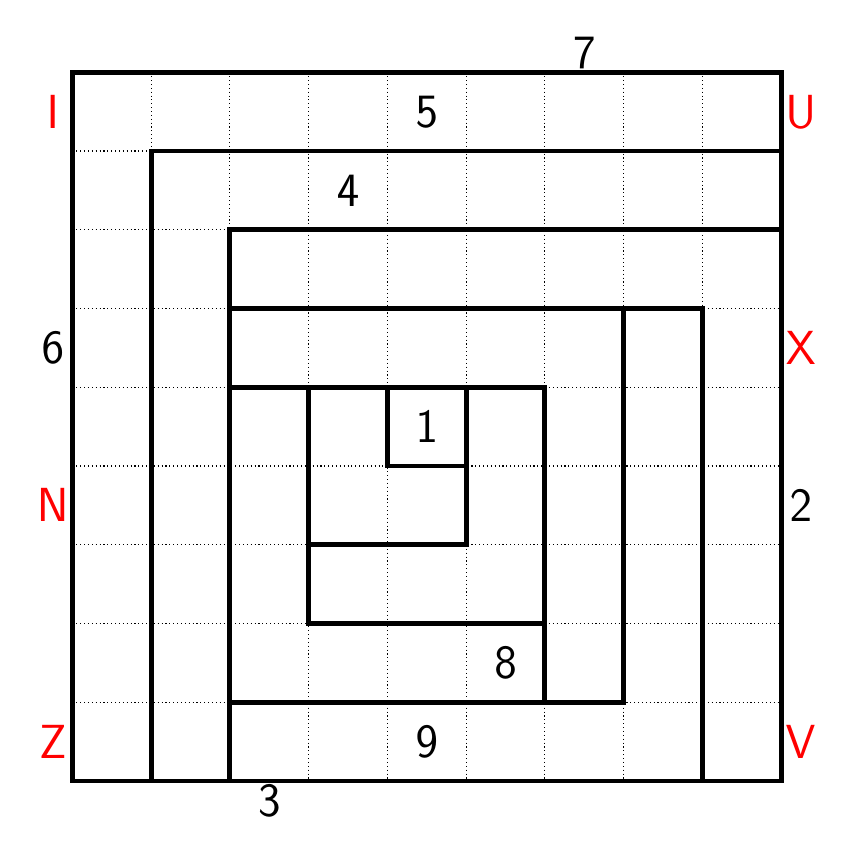
\begin{tikzpicture}
\drawthick (0,8)--++(0,1)--++(9,0)--++(0,-1)--++(-8,0)--++(0,-8)--++(-1,0)--cycle;
    \drawthick (1,7)--++(0,1)--++(8,0)--++(0,-1)--++(-7,0)--++(0,-7)--++(-1,0)--cycle;
    \drawthick (8,6)--++(-6,0)--++(0,1)--++(7,0)--++(0,-7)--++(-1,0)--cycle;
    \drawthick (7,0)--++(-5,0)--++(0,1)--++(5,0)--++(0,5)--++(1,0)--++(0,-6)--cycle;
    \drawthick (6,5)--++(-4,0)--++(0,1)--++(5,0)--++(0,-5)--++(-1,0)--cycle;
    \drawthick (2,1)--++(0,4)--++(1,0)--++(0,-3)--++(3,0)--++(0,-1)--cycle;
    \drawthick (5,2)--++(-2,0)--++(0,1)--++(2,0)--++(0,2)--++(1,0)--++(0,-3)--cycle;
    \drawthick (3,3)--++(0,2)--++(1,0)--++(0,-1)--++(1,0)--++(0,-1)--cycle;\drawgriddotted{9}
\numbersquare{1}{5}{5}\numbersquare{9}{5}{1}\numbersquare{8}{6}{2}\numbersquare{4}{4}{8}\numbersquare{5}{5}{9}\numbersquare{3}{3.0}{0.25}\numbersquare{2}{9.75}{4.0}\numbersquare{6}{0.25}{6.0}\numbersquare{7}{7.0}{9.75}\numbersquare{\textcolor{red}{I}}{0.25}{9.0}\numbersquare{\textcolor{red}{N}}{0.25}{4.0}\numbersquare{\textcolor{red}{Z}}{0.25}{1.0}\numbersquare{\textcolor{red}{V}}{9.75}{1.0}\numbersquare{\textcolor{red}{X}}{9.75}{6.0}\numbersquare{\textcolor{red}{U}}{9.75}{9.0}\end{tikzpicture}}
\vspace{1pc}\noindent{\large \texttt{\string{1:1, 2:$\sqcup$, 3:$\sqcup$, 4:$\sqcup$, 5:$\sqcup$, 6:$\sqcup$, 7:$\sqcup$, 8:$\sqcup$, 9:6\string}}}

\medskip\noindent{\large \texttt{hook 4 is too small for digit 8}}

\clearpage\resizebox{29.5pc}{!}{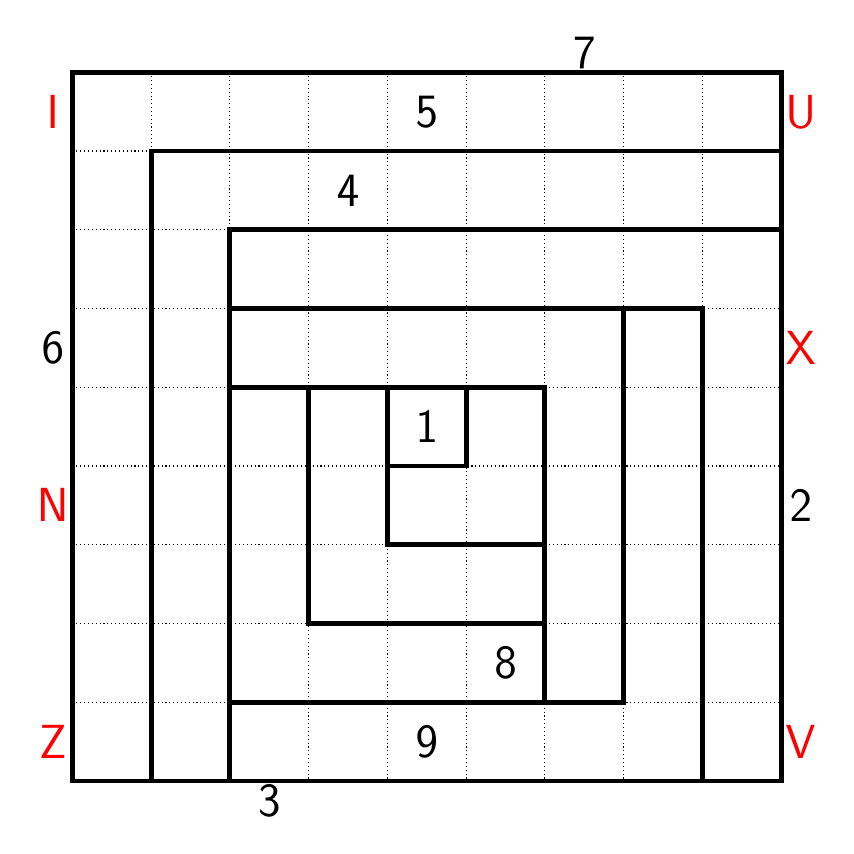
\begin{tikzpicture}
\drawthick (0,8)--++(0,1)--++(9,0)--++(0,-1)--++(-8,0)--++(0,-8)--++(-1,0)--cycle;
    \drawthick (1,7)--++(0,1)--++(8,0)--++(0,-1)--++(-7,0)--++(0,-7)--++(-1,0)--cycle;
    \drawthick (8,6)--++(-6,0)--++(0,1)--++(7,0)--++(0,-7)--++(-1,0)--cycle;
    \drawthick (7,0)--++(-5,0)--++(0,1)--++(5,0)--++(0,5)--++(1,0)--++(0,-6)--cycle;
    \drawthick (6,5)--++(-4,0)--++(0,1)--++(5,0)--++(0,-5)--++(-1,0)--cycle;
    \drawthick (2,1)--++(0,4)--++(1,0)--++(0,-3)--++(3,0)--++(0,-1)--cycle;
    \drawthick (3,2)--++(0,3)--++(1,0)--++(0,-2)--++(2,0)--++(0,-1)--cycle;
    \drawthick (5,3)--++(-1,0)--++(0,1)--++(1,0)--++(0,1)--++(1,0)--++(0,-2)--cycle;\drawgriddotted{9}
\numbersquare{1}{5}{5}\numbersquare{9}{5}{1}\numbersquare{8}{6}{2}\numbersquare{4}{4}{8}\numbersquare{5}{5}{9}\numbersquare{3}{3.0}{0.25}\numbersquare{2}{9.75}{4.0}\numbersquare{6}{0.25}{6.0}\numbersquare{7}{7.0}{9.75}\numbersquare{\textcolor{red}{I}}{0.25}{9.0}\numbersquare{\textcolor{red}{N}}{0.25}{4.0}\numbersquare{\textcolor{red}{Z}}{0.25}{1.0}\numbersquare{\textcolor{red}{V}}{9.75}{1.0}\numbersquare{\textcolor{red}{X}}{9.75}{6.0}\numbersquare{\textcolor{red}{U}}{9.75}{9.0}\end{tikzpicture}}
\vspace{1pc}\noindent{\large \texttt{\string{1:1, 2:$\sqcup$, 3:$\sqcup$, 4:$\sqcup$, 5:$\sqcup$, 6:$\sqcup$, 7:$\sqcup$, 8:$\sqcup$, 9:6\string}}}

\medskip\noindent{\large \texttt{hook 4 is too small for digit 8}}

\clearpage\resizebox{29.5pc}{!}{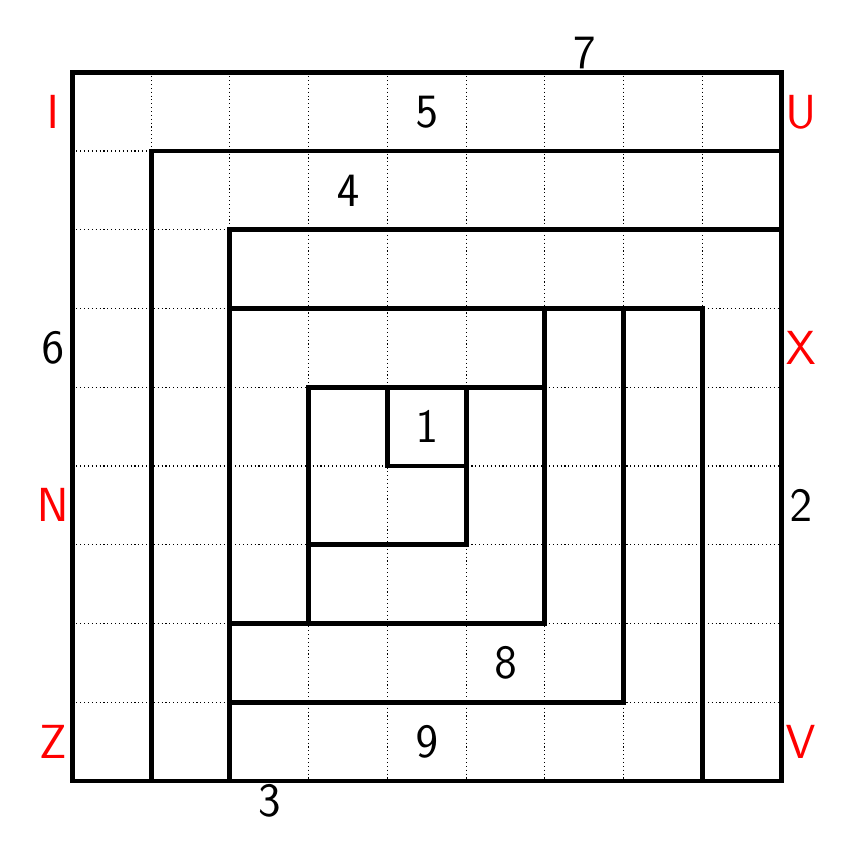
\begin{tikzpicture}
\drawthick (0,8)--++(0,1)--++(9,0)--++(0,-1)--++(-8,0)--++(0,-8)--++(-1,0)--cycle;
    \drawthick (1,7)--++(0,1)--++(8,0)--++(0,-1)--++(-7,0)--++(0,-7)--++(-1,0)--cycle;
    \drawthick (8,6)--++(-6,0)--++(0,1)--++(7,0)--++(0,-7)--++(-1,0)--cycle;
    \drawthick (7,0)--++(-5,0)--++(0,1)--++(5,0)--++(0,5)--++(1,0)--++(0,-6)--cycle;
    \drawthick (6,1)--++(-4,0)--++(0,1)--++(4,0)--++(0,4)--++(1,0)--++(0,-5)--cycle;
    \drawthick (2,5)--++(0,1)--++(4,0)--++(0,-1)--++(-3,0)--++(0,-3)--++(-1,0)--cycle;
    \drawthick (5,2)--++(-2,0)--++(0,1)--++(2,0)--++(0,2)--++(1,0)--++(0,-3)--cycle;
    \drawthick (3,3)--++(0,2)--++(1,0)--++(0,-1)--++(1,0)--++(0,-1)--cycle;\drawgriddotted{9}
\numbersquare{1}{5}{5}\numbersquare{9}{5}{1}\numbersquare{8}{6}{2}\numbersquare{4}{4}{8}\numbersquare{5}{5}{9}\numbersquare{3}{3.0}{0.25}\numbersquare{2}{9.75}{4.0}\numbersquare{6}{0.25}{6.0}\numbersquare{7}{7.0}{9.75}\numbersquare{\textcolor{red}{I}}{0.25}{9.0}\numbersquare{\textcolor{red}{N}}{0.25}{4.0}\numbersquare{\textcolor{red}{Z}}{0.25}{1.0}\numbersquare{\textcolor{red}{V}}{9.75}{1.0}\numbersquare{\textcolor{red}{X}}{9.75}{6.0}\numbersquare{\textcolor{red}{U}}{9.75}{9.0}\end{tikzpicture}}
\vspace{1pc}\noindent{\large \texttt{\string{1:1, 2:[2, 3], 3:4, 4:8, 5:9, 6:4, 7:7, 8:5, 9:6\string}}}

\medskip\noindent{\large \texttt{digits 3,6 are fighting over hook 4}}

\clearpage\resizebox{29.5pc}{!}{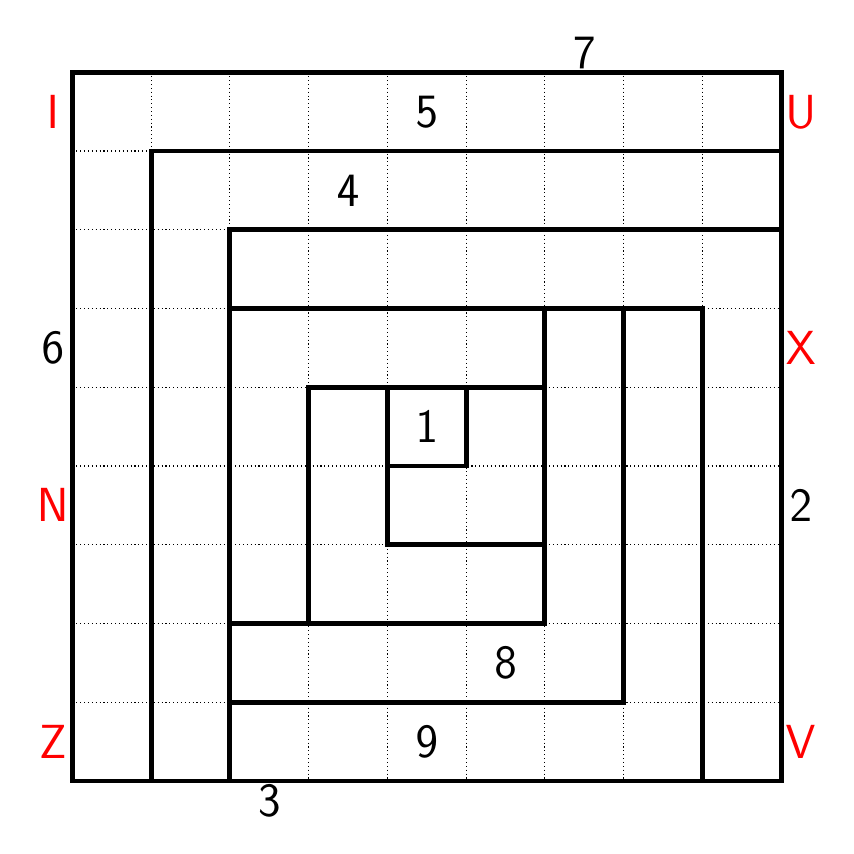
\begin{tikzpicture}
\drawthick (0,8)--++(0,1)--++(9,0)--++(0,-1)--++(-8,0)--++(0,-8)--++(-1,0)--cycle;
    \drawthick (1,7)--++(0,1)--++(8,0)--++(0,-1)--++(-7,0)--++(0,-7)--++(-1,0)--cycle;
    \drawthick (8,6)--++(-6,0)--++(0,1)--++(7,0)--++(0,-7)--++(-1,0)--cycle;
    \drawthick (7,0)--++(-5,0)--++(0,1)--++(5,0)--++(0,5)--++(1,0)--++(0,-6)--cycle;
    \drawthick (6,1)--++(-4,0)--++(0,1)--++(4,0)--++(0,4)--++(1,0)--++(0,-5)--cycle;
    \drawthick (2,5)--++(0,1)--++(4,0)--++(0,-1)--++(-3,0)--++(0,-3)--++(-1,0)--cycle;
    \drawthick (3,2)--++(0,3)--++(1,0)--++(0,-2)--++(2,0)--++(0,-1)--cycle;
    \drawthick (5,3)--++(-1,0)--++(0,1)--++(1,0)--++(0,1)--++(1,0)--++(0,-2)--cycle;\drawgriddotted{9}
\numbersquare{1}{5}{5}\numbersquare{9}{5}{1}\numbersquare{8}{6}{2}\numbersquare{4}{4}{8}\numbersquare{5}{5}{9}\numbersquare{3}{3.0}{0.25}\numbersquare{2}{9.75}{4.0}\numbersquare{6}{0.25}{6.0}\numbersquare{7}{7.0}{9.75}\numbersquare{\textcolor{red}{I}}{0.25}{9.0}\numbersquare{\textcolor{red}{N}}{0.25}{4.0}\numbersquare{\textcolor{red}{Z}}{0.25}{1.0}\numbersquare{\textcolor{red}{V}}{9.75}{1.0}\numbersquare{\textcolor{red}{X}}{9.75}{6.0}\numbersquare{\textcolor{red}{U}}{9.75}{9.0}\end{tikzpicture}}
\vspace{1pc}\noindent{\large \texttt{\string{1:1, 2:[2, 3], 3:4, 4:8, 5:9, 6:4, 7:7, 8:5, 9:6\string}}}

\medskip\noindent{\large \texttt{digits 3,6 are fighting over hook 4}}

\clearpage\resizebox{29.5pc}{!}{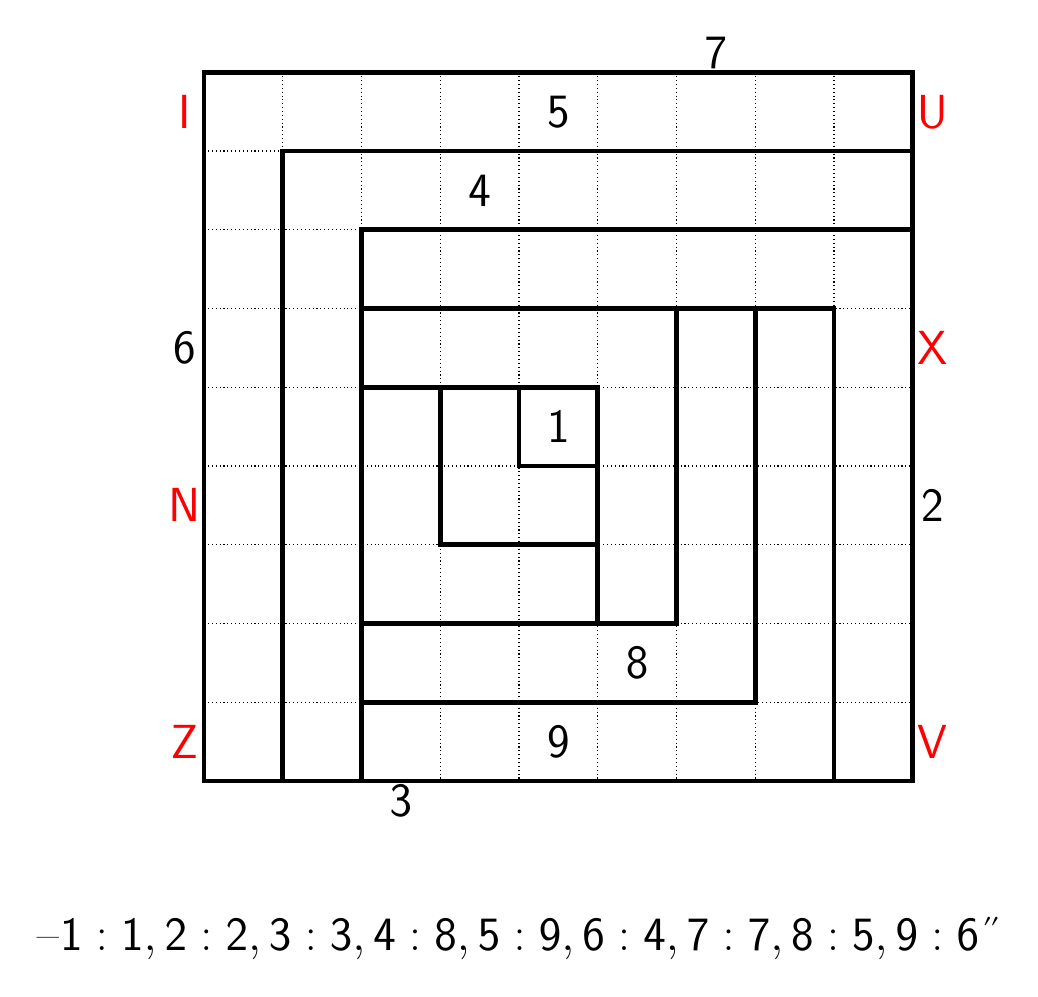
\begin{tikzpicture}
\drawthick (0,8)--++(0,1)--++(9,0)--++(0,-1)--++(-8,0)--++(0,-8)--++(-1,0)--cycle;
    \drawthick (1,7)--++(0,1)--++(8,0)--++(0,-1)--++(-7,0)--++(0,-7)--++(-1,0)--cycle;
    \drawthick (8,6)--++(-6,0)--++(0,1)--++(7,0)--++(0,-7)--++(-1,0)--cycle;
    \drawthick (7,0)--++(-5,0)--++(0,1)--++(5,0)--++(0,5)--++(1,0)--++(0,-6)--cycle;
    \drawthick (6,1)--++(-4,0)--++(0,1)--++(4,0)--++(0,4)--++(1,0)--++(0,-5)--cycle;
    \drawthick (5,5)--++(-3,0)--++(0,1)--++(4,0)--++(0,-4)--++(-1,0)--cycle;
    \drawthick (2,2)--++(0,3)--++(1,0)--++(0,-2)--++(2,0)--++(0,-1)--cycle;
    \drawthick (3,3)--++(0,2)--++(1,0)--++(0,-1)--++(1,0)--++(0,-1)--cycle;\drawgriddotted{9}
\numbersquare{1}{5}{5}\numbersquare{9}{5}{1}\numbersquare{8}{6}{2}\numbersquare{4}{4}{8}\numbersquare{5}{5}{9}\numbersquare{3}{3.0}{0.25}\numbersquare{2}{9.75}{4.0}\numbersquare{6}{0.25}{6.0}\numbersquare{7}{7.0}{9.75}\numbersquare{\textcolor{red}{I}}{0.25}{9.0}\numbersquare{\textcolor{red}{N}}{0.25}{4.0}\numbersquare{\textcolor{red}{Z}}{0.25}{1.0}\numbersquare{\textcolor{red}{V}}{9.75}{1.0}\numbersquare{\textcolor{red}{X}}{9.75}{6.0}\numbersquare{\textcolor{red}{U}}{9.75}{9.0}\numbersquare{\string{1:1, 2:2, 3:3, 4:8, 5:9, 6:4, 7:7, 8:5, 9:6\string}}{5-.5}{-1-.5}
\end{tikzpicture}}\,
\clearpage\resizebox{29.5pc}{!}{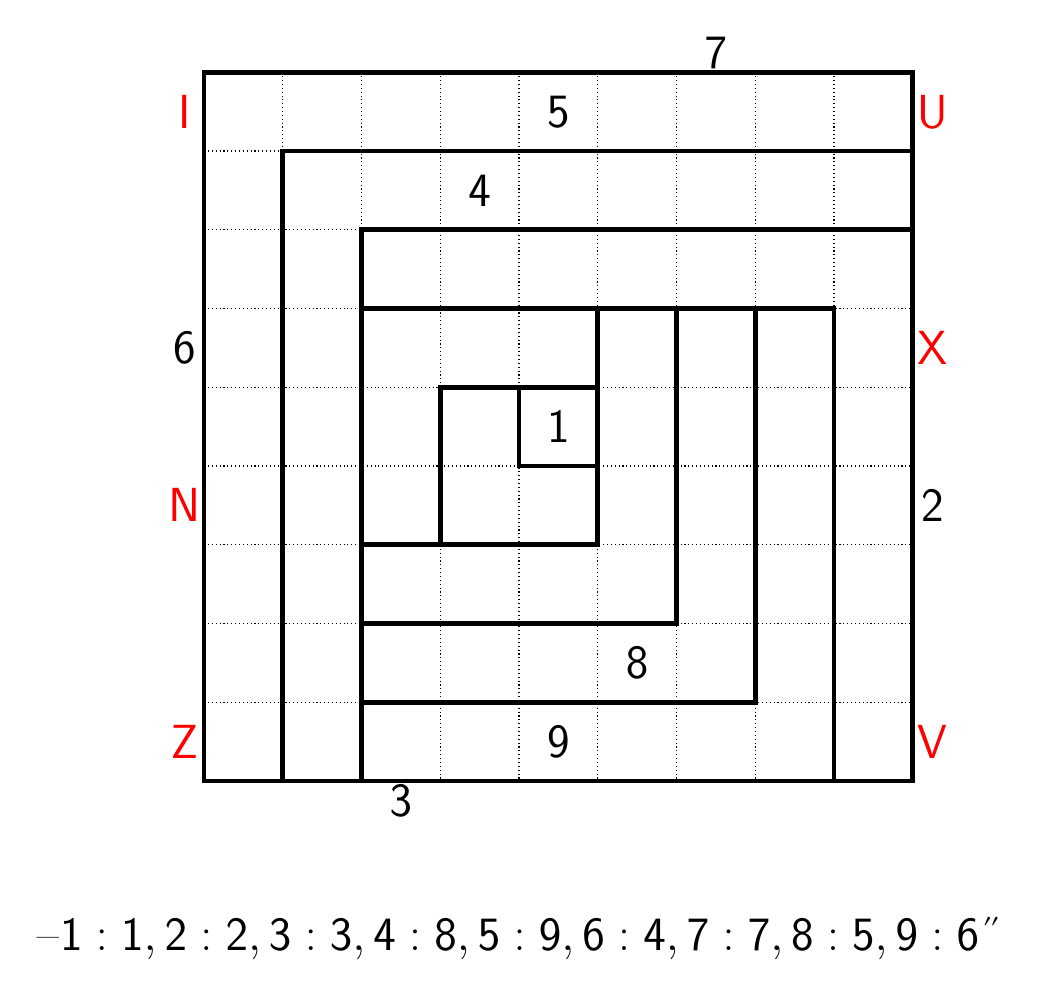
\begin{tikzpicture}
\drawthick (0,8)--++(0,1)--++(9,0)--++(0,-1)--++(-8,0)--++(0,-8)--++(-1,0)--cycle;
    \drawthick (1,7)--++(0,1)--++(8,0)--++(0,-1)--++(-7,0)--++(0,-7)--++(-1,0)--cycle;
    \drawthick (8,6)--++(-6,0)--++(0,1)--++(7,0)--++(0,-7)--++(-1,0)--cycle;
    \drawthick (7,0)--++(-5,0)--++(0,1)--++(5,0)--++(0,5)--++(1,0)--++(0,-6)--cycle;
    \drawthick (6,1)--++(-4,0)--++(0,1)--++(4,0)--++(0,4)--++(1,0)--++(0,-5)--cycle;
    \drawthick (5,2)--++(-3,0)--++(0,1)--++(3,0)--++(0,3)--++(1,0)--++(0,-4)--cycle;
    \drawthick (2,5)--++(0,1)--++(3,0)--++(0,-1)--++(-2,0)--++(0,-2)--++(-1,0)--cycle;
    \drawthick (3,3)--++(0,2)--++(1,0)--++(0,-1)--++(1,0)--++(0,-1)--cycle;\drawgriddotted{9}
\numbersquare{1}{5}{5}\numbersquare{9}{5}{1}\numbersquare{8}{6}{2}\numbersquare{4}{4}{8}\numbersquare{5}{5}{9}\numbersquare{3}{3.0}{0.25}\numbersquare{2}{9.75}{4.0}\numbersquare{6}{0.25}{6.0}\numbersquare{7}{7.0}{9.75}\numbersquare{\textcolor{red}{I}}{0.25}{9.0}\numbersquare{\textcolor{red}{N}}{0.25}{4.0}\numbersquare{\textcolor{red}{Z}}{0.25}{1.0}\numbersquare{\textcolor{red}{V}}{9.75}{1.0}\numbersquare{\textcolor{red}{X}}{9.75}{6.0}\numbersquare{\textcolor{red}{U}}{9.75}{9.0}\numbersquare{\string{1:1, 2:2, 3:3, 4:8, 5:9, 6:4, 7:7, 8:5, 9:6\string}}{5-.5}{-1-.5}
\end{tikzpicture}}\,
\clearpage\resizebox{29.5pc}{!}{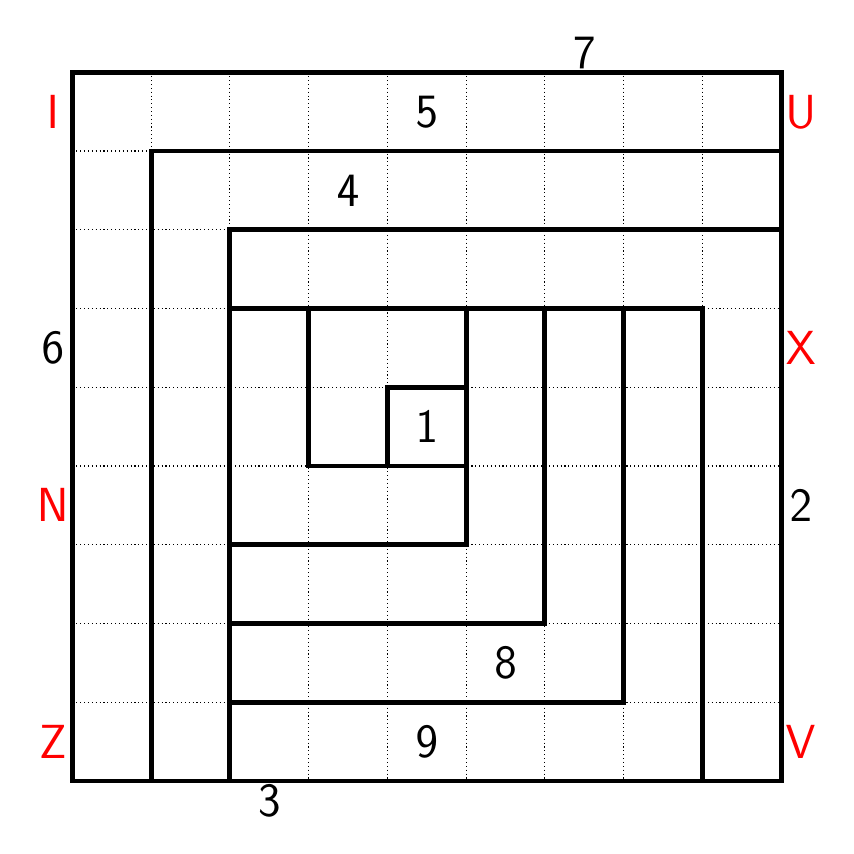
\begin{tikzpicture}
\drawthick (0,8)--++(0,1)--++(9,0)--++(0,-1)--++(-8,0)--++(0,-8)--++(-1,0)--cycle;
    \drawthick (1,7)--++(0,1)--++(8,0)--++(0,-1)--++(-7,0)--++(0,-7)--++(-1,0)--cycle;
    \drawthick (8,6)--++(-6,0)--++(0,1)--++(7,0)--++(0,-7)--++(-1,0)--cycle;
    \drawthick (7,0)--++(-5,0)--++(0,1)--++(5,0)--++(0,5)--++(1,0)--++(0,-6)--cycle;
    \drawthick (6,1)--++(-4,0)--++(0,1)--++(4,0)--++(0,4)--++(1,0)--++(0,-5)--cycle;
    \drawthick (5,2)--++(-3,0)--++(0,1)--++(3,0)--++(0,3)--++(1,0)--++(0,-4)--cycle;
    \drawthick (2,3)--++(0,3)--++(1,0)--++(0,-2)--++(2,0)--++(0,-1)--cycle;
    \drawthick (3,5)--++(0,1)--++(2,0)--++(0,-1)--++(-1,0)--++(0,-1)--++(-1,0)--cycle;\drawgriddotted{9}
\numbersquare{1}{5}{5}\numbersquare{9}{5}{1}\numbersquare{8}{6}{2}\numbersquare{4}{4}{8}\numbersquare{5}{5}{9}\numbersquare{3}{3.0}{0.25}\numbersquare{2}{9.75}{4.0}\numbersquare{6}{0.25}{6.0}\numbersquare{7}{7.0}{9.75}\numbersquare{\textcolor{red}{I}}{0.25}{9.0}\numbersquare{\textcolor{red}{N}}{0.25}{4.0}\numbersquare{\textcolor{red}{Z}}{0.25}{1.0}\numbersquare{\textcolor{red}{V}}{9.75}{1.0}\numbersquare{\textcolor{red}{X}}{9.75}{6.0}\numbersquare{\textcolor{red}{U}}{9.75}{9.0}\end{tikzpicture}}
\vspace{1pc}\noindent{\large \texttt{\string{1:1, 2:3, 3:3, 4:8, 5:9, 6:4, 7:7, 8:5, 9:6\string}}}

\medskip\noindent{\large \texttt{digits 2,3 are fighting over hook 3}}

\clearpage\resizebox{29.5pc}{!}{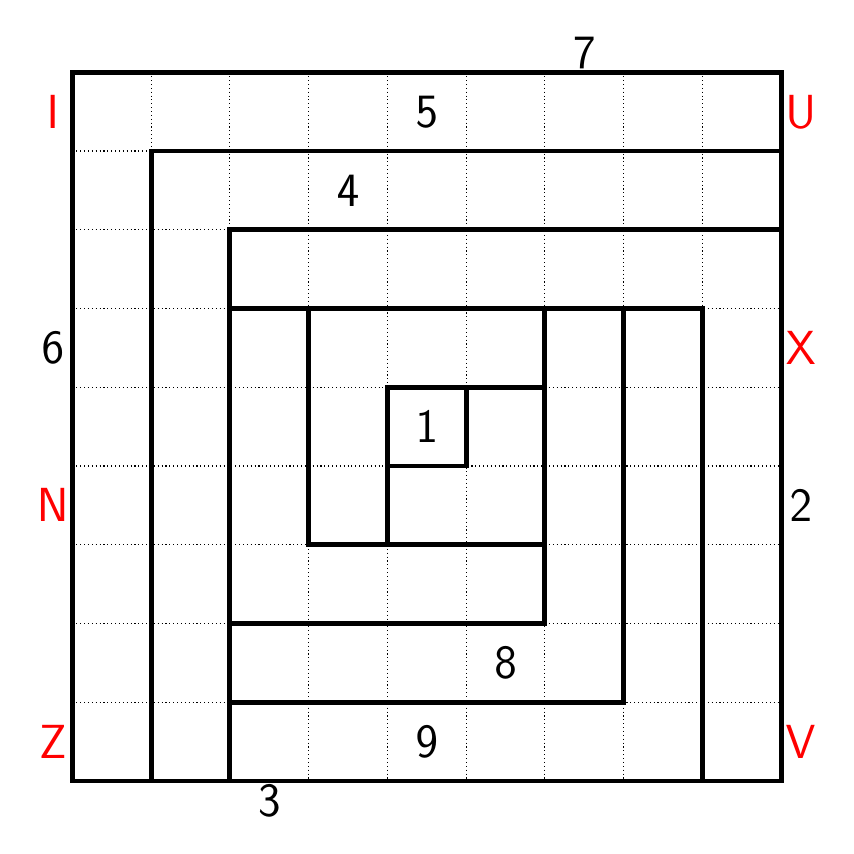
\begin{tikzpicture}
\drawthick (0,8)--++(0,1)--++(9,0)--++(0,-1)--++(-8,0)--++(0,-8)--++(-1,0)--cycle;
    \drawthick (1,7)--++(0,1)--++(8,0)--++(0,-1)--++(-7,0)--++(0,-7)--++(-1,0)--cycle;
    \drawthick (8,6)--++(-6,0)--++(0,1)--++(7,0)--++(0,-7)--++(-1,0)--cycle;
    \drawthick (7,0)--++(-5,0)--++(0,1)--++(5,0)--++(0,5)--++(1,0)--++(0,-6)--cycle;
    \drawthick (6,1)--++(-4,0)--++(0,1)--++(4,0)--++(0,4)--++(1,0)--++(0,-5)--cycle;
    \drawthick (2,2)--++(0,4)--++(1,0)--++(0,-3)--++(3,0)--++(0,-1)--cycle;
    \drawthick (3,5)--++(0,1)--++(3,0)--++(0,-1)--++(-2,0)--++(0,-2)--++(-1,0)--cycle;
    \drawthick (5,3)--++(-1,0)--++(0,1)--++(1,0)--++(0,1)--++(1,0)--++(0,-2)--cycle;\drawgriddotted{9}
\numbersquare{1}{5}{5}\numbersquare{9}{5}{1}\numbersquare{8}{6}{2}\numbersquare{4}{4}{8}\numbersquare{5}{5}{9}\numbersquare{3}{3.0}{0.25}\numbersquare{2}{9.75}{4.0}\numbersquare{6}{0.25}{6.0}\numbersquare{7}{7.0}{9.75}\numbersquare{\textcolor{red}{I}}{0.25}{9.0}\numbersquare{\textcolor{red}{N}}{0.25}{4.0}\numbersquare{\textcolor{red}{Z}}{0.25}{1.0}\numbersquare{\textcolor{red}{V}}{9.75}{1.0}\numbersquare{\textcolor{red}{X}}{9.75}{6.0}\numbersquare{\textcolor{red}{U}}{9.75}{9.0}\end{tikzpicture}}
\vspace{1pc}\noindent{\large \texttt{\string{1:1, 2:[2, 3], 3:4, 4:8, 5:9, 6:4, 7:7, 8:5, 9:6\string}}}

\medskip\noindent{\large \texttt{digits 3,6 are fighting over hook 4}}

\clearpage\resizebox{29.5pc}{!}{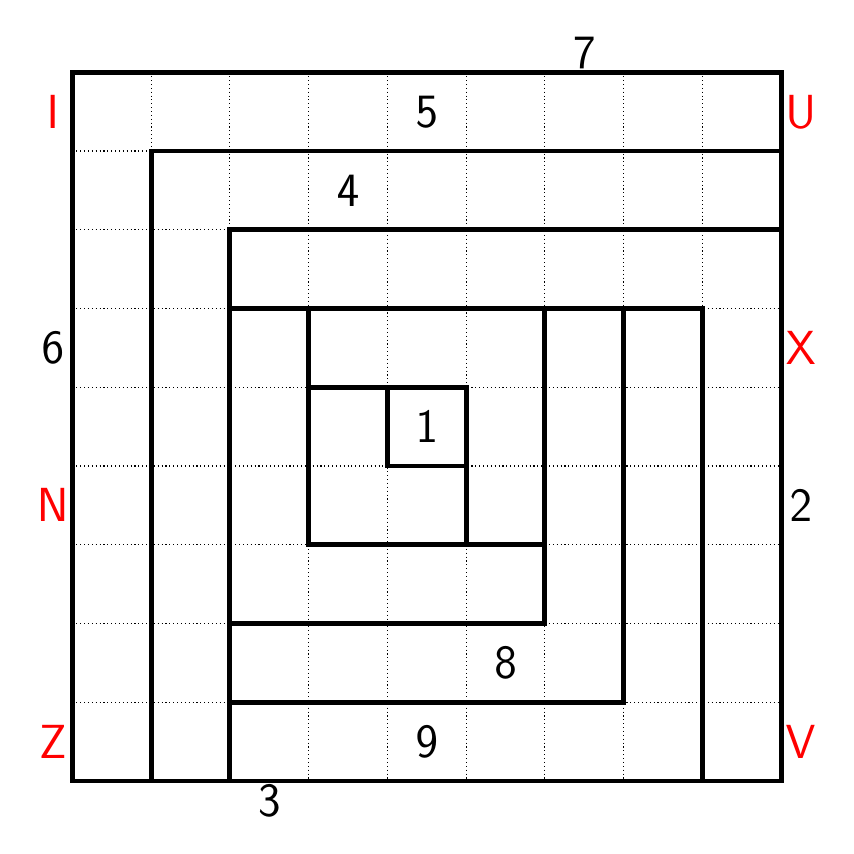
\begin{tikzpicture}
\drawthick (0,8)--++(0,1)--++(9,0)--++(0,-1)--++(-8,0)--++(0,-8)--++(-1,0)--cycle;
    \drawthick (1,7)--++(0,1)--++(8,0)--++(0,-1)--++(-7,0)--++(0,-7)--++(-1,0)--cycle;
    \drawthick (8,6)--++(-6,0)--++(0,1)--++(7,0)--++(0,-7)--++(-1,0)--cycle;
    \drawthick (7,0)--++(-5,0)--++(0,1)--++(5,0)--++(0,5)--++(1,0)--++(0,-6)--cycle;
    \drawthick (6,1)--++(-4,0)--++(0,1)--++(4,0)--++(0,4)--++(1,0)--++(0,-5)--cycle;
    \drawthick (2,2)--++(0,4)--++(1,0)--++(0,-3)--++(3,0)--++(0,-1)--cycle;
    \drawthick (5,5)--++(-2,0)--++(0,1)--++(3,0)--++(0,-3)--++(-1,0)--cycle;
    \drawthick (3,3)--++(0,2)--++(1,0)--++(0,-1)--++(1,0)--++(0,-1)--cycle;\drawgriddotted{9}
\numbersquare{1}{5}{5}\numbersquare{9}{5}{1}\numbersquare{8}{6}{2}\numbersquare{4}{4}{8}\numbersquare{5}{5}{9}\numbersquare{3}{3.0}{0.25}\numbersquare{2}{9.75}{4.0}\numbersquare{6}{0.25}{6.0}\numbersquare{7}{7.0}{9.75}\numbersquare{\textcolor{red}{I}}{0.25}{9.0}\numbersquare{\textcolor{red}{N}}{0.25}{4.0}\numbersquare{\textcolor{red}{Z}}{0.25}{1.0}\numbersquare{\textcolor{red}{V}}{9.75}{1.0}\numbersquare{\textcolor{red}{X}}{9.75}{6.0}\numbersquare{\textcolor{red}{U}}{9.75}{9.0}\end{tikzpicture}}
\vspace{1pc}\noindent{\large \texttt{\string{1:1, 2:[2, 3], 3:4, 4:8, 5:9, 6:4, 7:7, 8:5, 9:6\string}}}

\medskip\noindent{\large \texttt{digits 3,6 are fighting over hook 4}}

\clearpage\resizebox{29.5pc}{!}{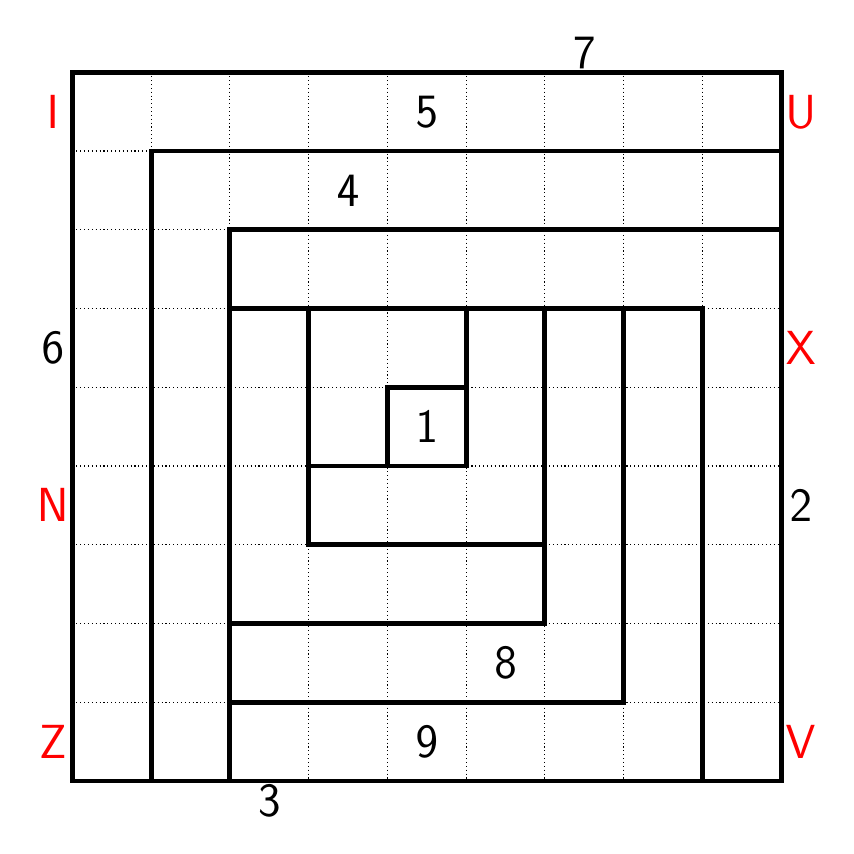
\begin{tikzpicture}
\drawthick (0,8)--++(0,1)--++(9,0)--++(0,-1)--++(-8,0)--++(0,-8)--++(-1,0)--cycle;
    \drawthick (1,7)--++(0,1)--++(8,0)--++(0,-1)--++(-7,0)--++(0,-7)--++(-1,0)--cycle;
    \drawthick (8,6)--++(-6,0)--++(0,1)--++(7,0)--++(0,-7)--++(-1,0)--cycle;
    \drawthick (7,0)--++(-5,0)--++(0,1)--++(5,0)--++(0,5)--++(1,0)--++(0,-6)--cycle;
    \drawthick (6,1)--++(-4,0)--++(0,1)--++(4,0)--++(0,4)--++(1,0)--++(0,-5)--cycle;
    \drawthick (2,2)--++(0,4)--++(1,0)--++(0,-3)--++(3,0)--++(0,-1)--cycle;
    \drawthick (5,3)--++(-2,0)--++(0,1)--++(2,0)--++(0,2)--++(1,0)--++(0,-3)--cycle;
    \drawthick (3,5)--++(0,1)--++(2,0)--++(0,-1)--++(-1,0)--++(0,-1)--++(-1,0)--cycle;\drawgriddotted{9}
\numbersquare{1}{5}{5}\numbersquare{9}{5}{1}\numbersquare{8}{6}{2}\numbersquare{4}{4}{8}\numbersquare{5}{5}{9}\numbersquare{3}{3.0}{0.25}\numbersquare{2}{9.75}{4.0}\numbersquare{6}{0.25}{6.0}\numbersquare{7}{7.0}{9.75}\numbersquare{\textcolor{red}{I}}{0.25}{9.0}\numbersquare{\textcolor{red}{N}}{0.25}{4.0}\numbersquare{\textcolor{red}{Z}}{0.25}{1.0}\numbersquare{\textcolor{red}{V}}{9.75}{1.0}\numbersquare{\textcolor{red}{X}}{9.75}{6.0}\numbersquare{\textcolor{red}{U}}{9.75}{9.0}\end{tikzpicture}}
\vspace{1pc}\noindent{\large \texttt{\string{1:1, 2:3, 3:4, 4:8, 5:9, 6:4, 7:7, 8:5, 9:6\string}}}

\medskip\noindent{\large \texttt{digits 3,6 are fighting over hook 4}}

\clearpage\resizebox{29.5pc}{!}{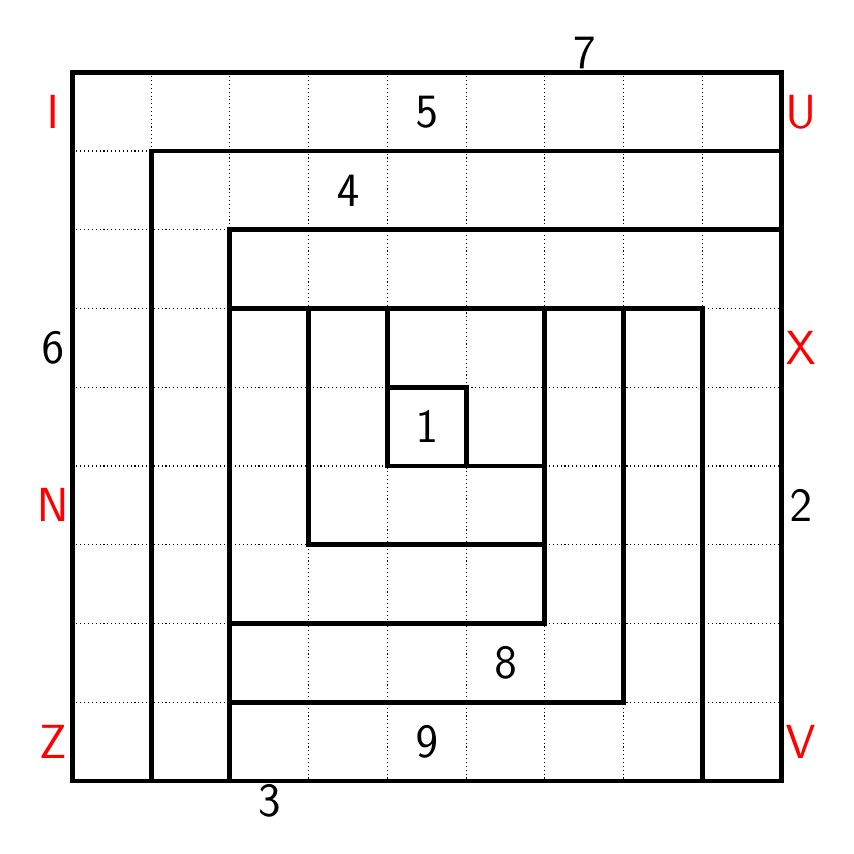
\begin{tikzpicture}
\drawthick (0,8)--++(0,1)--++(9,0)--++(0,-1)--++(-8,0)--++(0,-8)--++(-1,0)--cycle;
    \drawthick (1,7)--++(0,1)--++(8,0)--++(0,-1)--++(-7,0)--++(0,-7)--++(-1,0)--cycle;
    \drawthick (8,6)--++(-6,0)--++(0,1)--++(7,0)--++(0,-7)--++(-1,0)--cycle;
    \drawthick (7,0)--++(-5,0)--++(0,1)--++(5,0)--++(0,5)--++(1,0)--++(0,-6)--cycle;
    \drawthick (6,1)--++(-4,0)--++(0,1)--++(4,0)--++(0,4)--++(1,0)--++(0,-5)--cycle;
    \drawthick (2,2)--++(0,4)--++(1,0)--++(0,-3)--++(3,0)--++(0,-1)--cycle;
    \drawthick (3,3)--++(0,3)--++(1,0)--++(0,-2)--++(2,0)--++(0,-1)--cycle;
    \drawthick (5,5)--++(-1,0)--++(0,1)--++(2,0)--++(0,-2)--++(-1,0)--cycle;\drawgriddotted{9}
\numbersquare{1}{5}{5}\numbersquare{9}{5}{1}\numbersquare{8}{6}{2}\numbersquare{4}{4}{8}\numbersquare{5}{5}{9}\numbersquare{3}{3.0}{0.25}\numbersquare{2}{9.75}{4.0}\numbersquare{6}{0.25}{6.0}\numbersquare{7}{7.0}{9.75}\numbersquare{\textcolor{red}{I}}{0.25}{9.0}\numbersquare{\textcolor{red}{N}}{0.25}{4.0}\numbersquare{\textcolor{red}{Z}}{0.25}{1.0}\numbersquare{\textcolor{red}{V}}{9.75}{1.0}\numbersquare{\textcolor{red}{X}}{9.75}{6.0}\numbersquare{\textcolor{red}{U}}{9.75}{9.0}\end{tikzpicture}}
\vspace{1pc}\noindent{\large \texttt{\string{1:1, 2:3, 3:4, 4:8, 5:9, 6:4, 7:7, 8:5, 9:6\string}}}

\medskip\noindent{\large \texttt{digits 3,6 are fighting over hook 4}}

\clearpage\resizebox{29.5pc}{!}{\begin{tikzpicture}
\drawthick (0,8)--++(0,1)--++(9,0)--++(0,-1)--++(-8,0)--++(0,-8)--++(-1,0)--cycle;
    \drawthick (1,7)--++(0,1)--++(8,0)--++(0,-1)--++(-7,0)--++(0,-7)--++(-1,0)--cycle;
    \drawthick (8,6)--++(-6,0)--++(0,1)--++(7,0)--++(0,-7)--++(-1,0)--cycle;
    \drawthick (7,0)--++(-5,0)--++(0,1)--++(5,0)--++(0,5)--++(1,0)--++(0,-6)--cycle;
    \drawthick (2,1)--++(0,5)--++(1,0)--++(0,-4)--++(4,0)--++(0,-1)--cycle;
    \drawthick (3,5)--++(0,1)--++(4,0)--++(0,-1)--++(-3,0)--++(0,-3)--++(-1,0)--cycle;
    \drawthick (6,2)--++(-2,0)--++(0,1)--++(2,0)--++(0,2)--++(1,0)--++(0,-3)--cycle;
    \drawthick (5,3)--++(-1,0)--++(0,1)--++(1,0)--++(0,1)--++(1,0)--++(0,-2)--cycle;\drawgriddotted{9}
\numbersquare{1}{5}{5}\numbersquare{9}{5}{1}\numbersquare{8}{6}{2}\numbersquare{4}{4}{8}\numbersquare{5}{5}{9}\numbersquare{3}{3.0}{0.25}\numbersquare{2}{9.75}{4.0}\numbersquare{6}{0.25}{6.0}\numbersquare{7}{7.0}{9.75}\numbersquare{\textcolor{red}{I}}{0.25}{9.0}\numbersquare{\textcolor{red}{N}}{0.25}{4.0}\numbersquare{\textcolor{red}{Z}}{0.25}{1.0}\numbersquare{\textcolor{red}{V}}{9.75}{1.0}\numbersquare{\textcolor{red}{X}}{9.75}{6.0}\numbersquare{\textcolor{red}{U}}{9.75}{9.0}\end{tikzpicture}}
\vspace{1pc}\noindent{\large \texttt{\string{1:1, 2:[2, 3], 3:7, 4:8, 5:9, 6:4, 7:[], 8:5, 9:6\string}}}

\medskip\noindent{\large \texttt{digit(s) 7 cannot be assigned to any hook}}

\clearpage\resizebox{29.5pc}{!}{\begin{tikzpicture}
\drawthick (0,8)--++(0,1)--++(9,0)--++(0,-1)--++(-8,0)--++(0,-8)--++(-1,0)--cycle;
    \drawthick (1,7)--++(0,1)--++(8,0)--++(0,-1)--++(-7,0)--++(0,-7)--++(-1,0)--cycle;
    \drawthick (8,6)--++(-6,0)--++(0,1)--++(7,0)--++(0,-7)--++(-1,0)--cycle;
    \drawthick (7,0)--++(-5,0)--++(0,1)--++(5,0)--++(0,5)--++(1,0)--++(0,-6)--cycle;
    \drawthick (2,1)--++(0,5)--++(1,0)--++(0,-4)--++(4,0)--++(0,-1)--cycle;
    \drawthick (6,5)--++(-3,0)--++(0,1)--++(4,0)--++(0,-4)--++(-1,0)--cycle;
    \drawthick (5,2)--++(-2,0)--++(0,1)--++(2,0)--++(0,2)--++(1,0)--++(0,-3)--cycle;
    \drawthick (3,3)--++(0,2)--++(1,0)--++(0,-1)--++(1,0)--++(0,-1)--cycle;\drawgriddotted{9}
\numbersquare{1}{5}{5}\numbersquare{9}{5}{1}\numbersquare{8}{6}{2}\numbersquare{4}{4}{8}\numbersquare{5}{5}{9}\numbersquare{3}{3.0}{0.25}\numbersquare{2}{9.75}{4.0}\numbersquare{6}{0.25}{6.0}\numbersquare{7}{7.0}{9.75}\numbersquare{\textcolor{red}{I}}{0.25}{9.0}\numbersquare{\textcolor{red}{N}}{0.25}{4.0}\numbersquare{\textcolor{red}{Z}}{0.25}{1.0}\numbersquare{\textcolor{red}{V}}{9.75}{1.0}\numbersquare{\textcolor{red}{X}}{9.75}{6.0}\numbersquare{\textcolor{red}{U}}{9.75}{9.0}\end{tikzpicture}}
\vspace{1pc}\noindent{\large \texttt{\string{1:1, 2:[2, 3], 3:7, 4:8, 5:9, 6:4, 7:[], 8:5, 9:6\string}}}

\medskip\noindent{\large \texttt{digit(s) 7 cannot be assigned to any hook}}

\clearpage\resizebox{29.5pc}{!}{\begin{tikzpicture}
\drawthick (0,8)--++(0,1)--++(9,0)--++(0,-1)--++(-8,0)--++(0,-8)--++(-1,0)--cycle;
    \drawthick (1,7)--++(0,1)--++(8,0)--++(0,-1)--++(-7,0)--++(0,-7)--++(-1,0)--cycle;
    \drawthick (8,6)--++(-6,0)--++(0,1)--++(7,0)--++(0,-7)--++(-1,0)--cycle;
    \drawthick (7,0)--++(-5,0)--++(0,1)--++(5,0)--++(0,5)--++(1,0)--++(0,-6)--cycle;
    \drawthick (2,1)--++(0,5)--++(1,0)--++(0,-4)--++(4,0)--++(0,-1)--cycle;
    \drawthick (6,5)--++(-3,0)--++(0,1)--++(4,0)--++(0,-4)--++(-1,0)--cycle;
    \drawthick (3,2)--++(0,3)--++(1,0)--++(0,-2)--++(2,0)--++(0,-1)--cycle;
    \drawthick (5,3)--++(-1,0)--++(0,1)--++(1,0)--++(0,1)--++(1,0)--++(0,-2)--cycle;\drawgriddotted{9}
\numbersquare{1}{5}{5}\numbersquare{9}{5}{1}\numbersquare{8}{6}{2}\numbersquare{4}{4}{8}\numbersquare{5}{5}{9}\numbersquare{3}{3.0}{0.25}\numbersquare{2}{9.75}{4.0}\numbersquare{6}{0.25}{6.0}\numbersquare{7}{7.0}{9.75}\numbersquare{\textcolor{red}{I}}{0.25}{9.0}\numbersquare{\textcolor{red}{N}}{0.25}{4.0}\numbersquare{\textcolor{red}{Z}}{0.25}{1.0}\numbersquare{\textcolor{red}{V}}{9.75}{1.0}\numbersquare{\textcolor{red}{X}}{9.75}{6.0}\numbersquare{\textcolor{red}{U}}{9.75}{9.0}\end{tikzpicture}}
\vspace{1pc}\noindent{\large \texttt{\string{1:1, 2:[2, 3], 3:7, 4:8, 5:9, 6:4, 7:[], 8:5, 9:6\string}}}

\medskip\noindent{\large \texttt{digit(s) 7 cannot be assigned to any hook}}

\clearpage\resizebox{29.5pc}{!}{\begin{tikzpicture}
\drawthick (0,8)--++(0,1)--++(9,0)--++(0,-1)--++(-8,0)--++(0,-8)--++(-1,0)--cycle;
    \drawthick (1,7)--++(0,1)--++(8,0)--++(0,-1)--++(-7,0)--++(0,-7)--++(-1,0)--cycle;
    \drawthick (8,6)--++(-6,0)--++(0,1)--++(7,0)--++(0,-7)--++(-1,0)--cycle;
    \drawthick (7,0)--++(-5,0)--++(0,1)--++(5,0)--++(0,5)--++(1,0)--++(0,-6)--cycle;
    \drawthick (2,1)--++(0,5)--++(1,0)--++(0,-4)--++(4,0)--++(0,-1)--cycle;
    \drawthick (6,2)--++(-3,0)--++(0,1)--++(3,0)--++(0,3)--++(1,0)--++(0,-4)--cycle;
    \drawthick (3,5)--++(0,1)--++(3,0)--++(0,-1)--++(-2,0)--++(0,-2)--++(-1,0)--cycle;
    \drawthick (5,3)--++(-1,0)--++(0,1)--++(1,0)--++(0,1)--++(1,0)--++(0,-2)--cycle;\drawgriddotted{9}
\numbersquare{1}{5}{5}\numbersquare{9}{5}{1}\numbersquare{8}{6}{2}\numbersquare{4}{4}{8}\numbersquare{5}{5}{9}\numbersquare{3}{3.0}{0.25}\numbersquare{2}{9.75}{4.0}\numbersquare{6}{0.25}{6.0}\numbersquare{7}{7.0}{9.75}\numbersquare{\textcolor{red}{I}}{0.25}{9.0}\numbersquare{\textcolor{red}{N}}{0.25}{4.0}\numbersquare{\textcolor{red}{Z}}{0.25}{1.0}\numbersquare{\textcolor{red}{V}}{9.75}{1.0}\numbersquare{\textcolor{red}{X}}{9.75}{6.0}\numbersquare{\textcolor{red}{U}}{9.75}{9.0}\end{tikzpicture}}
\vspace{1pc}\noindent{\large \texttt{\string{1:1, 2:[2, 3], 3:7, 4:8, 5:9, 6:4, 7:[], 8:5, 9:6\string}}}

\medskip\noindent{\large \texttt{digit(s) 7 cannot be assigned to any hook}}

\clearpage\resizebox{29.5pc}{!}{\begin{tikzpicture}
\drawthick (0,8)--++(0,1)--++(9,0)--++(0,-1)--++(-8,0)--++(0,-8)--++(-1,0)--cycle;
    \drawthick (1,7)--++(0,1)--++(8,0)--++(0,-1)--++(-7,0)--++(0,-7)--++(-1,0)--cycle;
    \drawthick (8,6)--++(-6,0)--++(0,1)--++(7,0)--++(0,-7)--++(-1,0)--cycle;
    \drawthick (7,0)--++(-5,0)--++(0,1)--++(5,0)--++(0,5)--++(1,0)--++(0,-6)--cycle;
    \drawthick (2,1)--++(0,5)--++(1,0)--++(0,-4)--++(4,0)--++(0,-1)--cycle;
    \drawthick (6,2)--++(-3,0)--++(0,1)--++(3,0)--++(0,3)--++(1,0)--++(0,-4)--cycle;
    \drawthick (5,5)--++(-2,0)--++(0,1)--++(3,0)--++(0,-3)--++(-1,0)--cycle;
    \drawthick (3,3)--++(0,2)--++(1,0)--++(0,-1)--++(1,0)--++(0,-1)--cycle;\drawgriddotted{9}
\numbersquare{1}{5}{5}\numbersquare{9}{5}{1}\numbersquare{8}{6}{2}\numbersquare{4}{4}{8}\numbersquare{5}{5}{9}\numbersquare{3}{3.0}{0.25}\numbersquare{2}{9.75}{4.0}\numbersquare{6}{0.25}{6.0}\numbersquare{7}{7.0}{9.75}\numbersquare{\textcolor{red}{I}}{0.25}{9.0}\numbersquare{\textcolor{red}{N}}{0.25}{4.0}\numbersquare{\textcolor{red}{Z}}{0.25}{1.0}\numbersquare{\textcolor{red}{V}}{9.75}{1.0}\numbersquare{\textcolor{red}{X}}{9.75}{6.0}\numbersquare{\textcolor{red}{U}}{9.75}{9.0}\end{tikzpicture}}
\vspace{1pc}\noindent{\large \texttt{\string{1:1, 2:[2, 3], 3:7, 4:8, 5:9, 6:4, 7:[], 8:5, 9:6\string}}}

\medskip\noindent{\large \texttt{digit(s) 7 cannot be assigned to any hook}}

\clearpage\resizebox{29.5pc}{!}{\begin{tikzpicture}
\drawthick (0,8)--++(0,1)--++(9,0)--++(0,-1)--++(-8,0)--++(0,-8)--++(-1,0)--cycle;
    \drawthick (1,7)--++(0,1)--++(8,0)--++(0,-1)--++(-7,0)--++(0,-7)--++(-1,0)--cycle;
    \drawthick (8,6)--++(-6,0)--++(0,1)--++(7,0)--++(0,-7)--++(-1,0)--cycle;
    \drawthick (7,0)--++(-5,0)--++(0,1)--++(5,0)--++(0,5)--++(1,0)--++(0,-6)--cycle;
    \drawthick (2,1)--++(0,5)--++(1,0)--++(0,-4)--++(4,0)--++(0,-1)--cycle;
    \drawthick (6,2)--++(-3,0)--++(0,1)--++(3,0)--++(0,3)--++(1,0)--++(0,-4)--cycle;
    \drawthick (5,3)--++(-2,0)--++(0,1)--++(2,0)--++(0,2)--++(1,0)--++(0,-3)--cycle;
    \drawthick (3,5)--++(0,1)--++(2,0)--++(0,-1)--++(-1,0)--++(0,-1)--++(-1,0)--cycle;\drawgriddotted{9}
\numbersquare{1}{5}{5}\numbersquare{9}{5}{1}\numbersquare{8}{6}{2}\numbersquare{4}{4}{8}\numbersquare{5}{5}{9}\numbersquare{3}{3.0}{0.25}\numbersquare{2}{9.75}{4.0}\numbersquare{6}{0.25}{6.0}\numbersquare{7}{7.0}{9.75}\numbersquare{\textcolor{red}{I}}{0.25}{9.0}\numbersquare{\textcolor{red}{N}}{0.25}{4.0}\numbersquare{\textcolor{red}{Z}}{0.25}{1.0}\numbersquare{\textcolor{red}{V}}{9.75}{1.0}\numbersquare{\textcolor{red}{X}}{9.75}{6.0}\numbersquare{\textcolor{red}{U}}{9.75}{9.0}\end{tikzpicture}}
\vspace{1pc}\noindent{\large \texttt{\string{1:1, 2:3, 3:7, 4:8, 5:9, 6:4, 7:[], 8:5, 9:6\string}}}

\medskip\noindent{\large \texttt{digit(s) 7 cannot be assigned to any hook}}

\clearpage\resizebox{29.5pc}{!}{\begin{tikzpicture}
\drawthick (0,8)--++(0,1)--++(9,0)--++(0,-1)--++(-8,0)--++(0,-8)--++(-1,0)--cycle;
    \drawthick (1,7)--++(0,1)--++(8,0)--++(0,-1)--++(-7,0)--++(0,-7)--++(-1,0)--cycle;
    \drawthick (8,6)--++(-6,0)--++(0,1)--++(7,0)--++(0,-7)--++(-1,0)--cycle;
    \drawthick (7,0)--++(-5,0)--++(0,1)--++(5,0)--++(0,5)--++(1,0)--++(0,-6)--cycle;
    \drawthick (2,1)--++(0,5)--++(1,0)--++(0,-4)--++(4,0)--++(0,-1)--cycle;
    \drawthick (6,2)--++(-3,0)--++(0,1)--++(3,0)--++(0,3)--++(1,0)--++(0,-4)--cycle;
    \drawthick (3,3)--++(0,3)--++(1,0)--++(0,-2)--++(2,0)--++(0,-1)--cycle;
    \drawthick (5,5)--++(-1,0)--++(0,1)--++(2,0)--++(0,-2)--++(-1,0)--cycle;\drawgriddotted{9}
\numbersquare{1}{5}{5}\numbersquare{9}{5}{1}\numbersquare{8}{6}{2}\numbersquare{4}{4}{8}\numbersquare{5}{5}{9}\numbersquare{3}{3.0}{0.25}\numbersquare{2}{9.75}{4.0}\numbersquare{6}{0.25}{6.0}\numbersquare{7}{7.0}{9.75}\numbersquare{\textcolor{red}{I}}{0.25}{9.0}\numbersquare{\textcolor{red}{N}}{0.25}{4.0}\numbersquare{\textcolor{red}{Z}}{0.25}{1.0}\numbersquare{\textcolor{red}{V}}{9.75}{1.0}\numbersquare{\textcolor{red}{X}}{9.75}{6.0}\numbersquare{\textcolor{red}{U}}{9.75}{9.0}\end{tikzpicture}}
\vspace{1pc}\noindent{\large \texttt{\string{1:1, 2:3, 3:7, 4:8, 5:9, 6:4, 7:[], 8:5, 9:6\string}}}

\medskip\noindent{\large \texttt{digit(s) 7 cannot be assigned to any hook}}

\clearpage\resizebox{29.5pc}{!}{\begin{tikzpicture}
\drawthick (0,8)--++(0,1)--++(9,0)--++(0,-1)--++(-8,0)--++(0,-8)--++(-1,0)--cycle;
    \drawthick (1,7)--++(0,1)--++(8,0)--++(0,-1)--++(-7,0)--++(0,-7)--++(-1,0)--cycle;
    \drawthick (8,6)--++(-6,0)--++(0,1)--++(7,0)--++(0,-7)--++(-1,0)--cycle;
    \drawthick (7,0)--++(-5,0)--++(0,1)--++(5,0)--++(0,5)--++(1,0)--++(0,-6)--cycle;
    \drawthick (2,1)--++(0,5)--++(1,0)--++(0,-4)--++(4,0)--++(0,-1)--cycle;
    \drawthick (3,2)--++(0,4)--++(1,0)--++(0,-3)--++(3,0)--++(0,-1)--cycle;
    \drawthick (6,5)--++(-2,0)--++(0,1)--++(3,0)--++(0,-3)--++(-1,0)--cycle;
    \drawthick (5,3)--++(-1,0)--++(0,1)--++(1,0)--++(0,1)--++(1,0)--++(0,-2)--cycle;\drawgriddotted{9}
\numbersquare{1}{5}{5}\numbersquare{9}{5}{1}\numbersquare{8}{6}{2}\numbersquare{4}{4}{8}\numbersquare{5}{5}{9}\numbersquare{3}{3.0}{0.25}\numbersquare{2}{9.75}{4.0}\numbersquare{6}{0.25}{6.0}\numbersquare{7}{7.0}{9.75}\numbersquare{\textcolor{red}{I}}{0.25}{9.0}\numbersquare{\textcolor{red}{N}}{0.25}{4.0}\numbersquare{\textcolor{red}{Z}}{0.25}{1.0}\numbersquare{\textcolor{red}{V}}{9.75}{1.0}\numbersquare{\textcolor{red}{X}}{9.75}{6.0}\numbersquare{\textcolor{red}{U}}{9.75}{9.0}\end{tikzpicture}}
\vspace{1pc}\noindent{\large \texttt{\string{1:1, 2:[2, 3], 3:7, 4:8, 5:9, 6:4, 7:[], 8:5, 9:6\string}}}

\medskip\noindent{\large \texttt{digit(s) 7 cannot be assigned to any hook}}

\clearpage\resizebox{29.5pc}{!}{\begin{tikzpicture}
\drawthick (0,8)--++(0,1)--++(9,0)--++(0,-1)--++(-8,0)--++(0,-8)--++(-1,0)--cycle;
    \drawthick (1,7)--++(0,1)--++(8,0)--++(0,-1)--++(-7,0)--++(0,-7)--++(-1,0)--cycle;
    \drawthick (8,6)--++(-6,0)--++(0,1)--++(7,0)--++(0,-7)--++(-1,0)--cycle;
    \drawthick (7,0)--++(-5,0)--++(0,1)--++(5,0)--++(0,5)--++(1,0)--++(0,-6)--cycle;
    \drawthick (2,1)--++(0,5)--++(1,0)--++(0,-4)--++(4,0)--++(0,-1)--cycle;
    \drawthick (3,2)--++(0,4)--++(1,0)--++(0,-3)--++(3,0)--++(0,-1)--cycle;
    \drawthick (6,3)--++(-2,0)--++(0,1)--++(2,0)--++(0,2)--++(1,0)--++(0,-3)--cycle;
    \drawthick (5,5)--++(-1,0)--++(0,1)--++(2,0)--++(0,-2)--++(-1,0)--cycle;\drawgriddotted{9}
\numbersquare{1}{5}{5}\numbersquare{9}{5}{1}\numbersquare{8}{6}{2}\numbersquare{4}{4}{8}\numbersquare{5}{5}{9}\numbersquare{3}{3.0}{0.25}\numbersquare{2}{9.75}{4.0}\numbersquare{6}{0.25}{6.0}\numbersquare{7}{7.0}{9.75}\numbersquare{\textcolor{red}{I}}{0.25}{9.0}\numbersquare{\textcolor{red}{N}}{0.25}{4.0}\numbersquare{\textcolor{red}{Z}}{0.25}{1.0}\numbersquare{\textcolor{red}{V}}{9.75}{1.0}\numbersquare{\textcolor{red}{X}}{9.75}{6.0}\numbersquare{\textcolor{red}{U}}{9.75}{9.0}\end{tikzpicture}}
\vspace{1pc}\noindent{\large \texttt{\string{1:1, 2:3, 3:7, 4:8, 5:9, 6:4, 7:[], 8:5, 9:6\string}}}

\medskip\noindent{\large \texttt{digit(s) 7 cannot be assigned to any hook}}

\clearpage\resizebox{29.5pc}{!}{\begin{tikzpicture}
\drawthick (0,8)--++(0,1)--++(9,0)--++(0,-1)--++(-8,0)--++(0,-8)--++(-1,0)--cycle;
    \drawthick (1,7)--++(0,1)--++(8,0)--++(0,-1)--++(-7,0)--++(0,-7)--++(-1,0)--cycle;
    \drawthick (8,6)--++(-6,0)--++(0,1)--++(7,0)--++(0,-7)--++(-1,0)--cycle;
    \drawthick (2,0)--++(0,6)--++(1,0)--++(0,-5)--++(5,0)--++(0,-1)--cycle;
    \drawthick (3,5)--++(0,1)--++(5,0)--++(0,-1)--++(-4,0)--++(0,-4)--++(-1,0)--cycle;
    \drawthick (7,1)--++(-3,0)--++(0,1)--++(3,0)--++(0,3)--++(1,0)--++(0,-4)--cycle;
    \drawthick (6,2)--++(-2,0)--++(0,1)--++(2,0)--++(0,2)--++(1,0)--++(0,-3)--cycle;
    \drawthick (5,3)--++(-1,0)--++(0,1)--++(1,0)--++(0,1)--++(1,0)--++(0,-2)--cycle;\drawgriddotted{9}
\numbersquare{1}{5}{5}\numbersquare{9}{5}{1}\numbersquare{8}{6}{2}\numbersquare{4}{4}{8}\numbersquare{5}{5}{9}\numbersquare{3}{3.0}{0.25}\numbersquare{2}{9.75}{4.0}\numbersquare{6}{0.25}{6.0}\numbersquare{7}{7.0}{9.75}\numbersquare{\textcolor{red}{I}}{0.25}{9.0}\numbersquare{\textcolor{red}{N}}{0.25}{4.0}\numbersquare{\textcolor{red}{Z}}{0.25}{1.0}\numbersquare{\textcolor{red}{V}}{9.75}{1.0}\numbersquare{\textcolor{red}{X}}{9.75}{6.0}\numbersquare{\textcolor{red}{U}}{9.75}{9.0}\end{tikzpicture}}
\vspace{1pc}\noindent{\large \texttt{\string{1:1, 2:$\sqcup$, 3:$\sqcup$, 4:$\sqcup$, 5:$\sqcup$, 6:$\sqcup$, 7:$\sqcup$, 8:$\sqcup$, 9:6\string}}}

\medskip\noindent{\large \texttt{hook 4 is too small for digit 8}}

\clearpage\resizebox{29.5pc}{!}{\begin{tikzpicture}
\drawthick (0,8)--++(0,1)--++(9,0)--++(0,-1)--++(-8,0)--++(0,-8)--++(-1,0)--cycle;
    \drawthick (1,7)--++(0,1)--++(8,0)--++(0,-1)--++(-7,0)--++(0,-7)--++(-1,0)--cycle;
    \drawthick (8,6)--++(-6,0)--++(0,1)--++(7,0)--++(0,-7)--++(-1,0)--cycle;
    \drawthick (2,0)--++(0,6)--++(1,0)--++(0,-5)--++(5,0)--++(0,-1)--cycle;
    \drawthick (7,5)--++(-4,0)--++(0,1)--++(5,0)--++(0,-5)--++(-1,0)--cycle;
    \drawthick (6,1)--++(-3,0)--++(0,1)--++(3,0)--++(0,3)--++(1,0)--++(0,-4)--cycle;
    \drawthick (5,2)--++(-2,0)--++(0,1)--++(2,0)--++(0,2)--++(1,0)--++(0,-3)--cycle;
    \drawthick (3,3)--++(0,2)--++(1,0)--++(0,-1)--++(1,0)--++(0,-1)--cycle;\drawgriddotted{9}
\numbersquare{1}{5}{5}\numbersquare{9}{5}{1}\numbersquare{8}{6}{2}\numbersquare{4}{4}{8}\numbersquare{5}{5}{9}\numbersquare{3}{3.0}{0.25}\numbersquare{2}{9.75}{4.0}\numbersquare{6}{0.25}{6.0}\numbersquare{7}{7.0}{9.75}\numbersquare{\textcolor{red}{I}}{0.25}{9.0}\numbersquare{\textcolor{red}{N}}{0.25}{4.0}\numbersquare{\textcolor{red}{Z}}{0.25}{1.0}\numbersquare{\textcolor{red}{V}}{9.75}{1.0}\numbersquare{\textcolor{red}{X}}{9.75}{6.0}\numbersquare{\textcolor{red}{U}}{9.75}{9.0}\end{tikzpicture}}
\vspace{1pc}\noindent{\large \texttt{\string{1:1, 2:$\sqcup$, 3:$\sqcup$, 4:$\sqcup$, 5:$\sqcup$, 6:$\sqcup$, 7:$\sqcup$, 8:$\sqcup$, 9:6\string}}}

\medskip\noindent{\large \texttt{hook 4 is too small for digit 8}}

\clearpage\resizebox{29.5pc}{!}{\begin{tikzpicture}
\drawthick (0,8)--++(0,1)--++(9,0)--++(0,-1)--++(-8,0)--++(0,-8)--++(-1,0)--cycle;
    \drawthick (1,7)--++(0,1)--++(8,0)--++(0,-1)--++(-7,0)--++(0,-7)--++(-1,0)--cycle;
    \drawthick (8,6)--++(-6,0)--++(0,1)--++(7,0)--++(0,-7)--++(-1,0)--cycle;
    \drawthick (2,0)--++(0,6)--++(1,0)--++(0,-5)--++(5,0)--++(0,-1)--cycle;
    \drawthick (7,5)--++(-4,0)--++(0,1)--++(5,0)--++(0,-5)--++(-1,0)--cycle;
    \drawthick (6,1)--++(-3,0)--++(0,1)--++(3,0)--++(0,3)--++(1,0)--++(0,-4)--cycle;
    \drawthick (3,2)--++(0,3)--++(1,0)--++(0,-2)--++(2,0)--++(0,-1)--cycle;
    \drawthick (5,3)--++(-1,0)--++(0,1)--++(1,0)--++(0,1)--++(1,0)--++(0,-2)--cycle;\drawgriddotted{9}
\numbersquare{1}{5}{5}\numbersquare{9}{5}{1}\numbersquare{8}{6}{2}\numbersquare{4}{4}{8}\numbersquare{5}{5}{9}\numbersquare{3}{3.0}{0.25}\numbersquare{2}{9.75}{4.0}\numbersquare{6}{0.25}{6.0}\numbersquare{7}{7.0}{9.75}\numbersquare{\textcolor{red}{I}}{0.25}{9.0}\numbersquare{\textcolor{red}{N}}{0.25}{4.0}\numbersquare{\textcolor{red}{Z}}{0.25}{1.0}\numbersquare{\textcolor{red}{V}}{9.75}{1.0}\numbersquare{\textcolor{red}{X}}{9.75}{6.0}\numbersquare{\textcolor{red}{U}}{9.75}{9.0}\end{tikzpicture}}
\vspace{1pc}\noindent{\large \texttt{\string{1:1, 2:$\sqcup$, 3:$\sqcup$, 4:$\sqcup$, 5:$\sqcup$, 6:$\sqcup$, 7:$\sqcup$, 8:$\sqcup$, 9:6\string}}}

\medskip\noindent{\large \texttt{hook 4 is too small for digit 8}}

\clearpage\resizebox{29.5pc}{!}{\begin{tikzpicture}
\drawthick (0,8)--++(0,1)--++(9,0)--++(0,-1)--++(-8,0)--++(0,-8)--++(-1,0)--cycle;
    \drawthick (1,7)--++(0,1)--++(8,0)--++(0,-1)--++(-7,0)--++(0,-7)--++(-1,0)--cycle;
    \drawthick (8,6)--++(-6,0)--++(0,1)--++(7,0)--++(0,-7)--++(-1,0)--cycle;
    \drawthick (2,0)--++(0,6)--++(1,0)--++(0,-5)--++(5,0)--++(0,-1)--cycle;
    \drawthick (7,5)--++(-4,0)--++(0,1)--++(5,0)--++(0,-5)--++(-1,0)--cycle;
    \drawthick (3,1)--++(0,4)--++(1,0)--++(0,-3)--++(3,0)--++(0,-1)--cycle;
    \drawthick (6,2)--++(-2,0)--++(0,1)--++(2,0)--++(0,2)--++(1,0)--++(0,-3)--cycle;
    \drawthick (5,3)--++(-1,0)--++(0,1)--++(1,0)--++(0,1)--++(1,0)--++(0,-2)--cycle;\drawgriddotted{9}
\numbersquare{1}{5}{5}\numbersquare{9}{5}{1}\numbersquare{8}{6}{2}\numbersquare{4}{4}{8}\numbersquare{5}{5}{9}\numbersquare{3}{3.0}{0.25}\numbersquare{2}{9.75}{4.0}\numbersquare{6}{0.25}{6.0}\numbersquare{7}{7.0}{9.75}\numbersquare{\textcolor{red}{I}}{0.25}{9.0}\numbersquare{\textcolor{red}{N}}{0.25}{4.0}\numbersquare{\textcolor{red}{Z}}{0.25}{1.0}\numbersquare{\textcolor{red}{V}}{9.75}{1.0}\numbersquare{\textcolor{red}{X}}{9.75}{6.0}\numbersquare{\textcolor{red}{U}}{9.75}{9.0}\end{tikzpicture}}
\vspace{1pc}\noindent{\large \texttt{\string{1:1, 2:$\sqcup$, 3:$\sqcup$, 4:$\sqcup$, 5:$\sqcup$, 6:$\sqcup$, 7:$\sqcup$, 8:$\sqcup$, 9:6\string}}}

\medskip\noindent{\large \texttt{hook 4 is too small for digit 8}}

\clearpage\resizebox{29.5pc}{!}{\begin{tikzpicture}
\drawthick (0,8)--++(0,1)--++(9,0)--++(0,-1)--++(-8,0)--++(0,-8)--++(-1,0)--cycle;
    \drawthick (1,7)--++(0,1)--++(8,0)--++(0,-1)--++(-7,0)--++(0,-7)--++(-1,0)--cycle;
    \drawthick (8,6)--++(-6,0)--++(0,1)--++(7,0)--++(0,-7)--++(-1,0)--cycle;
    \drawthick (2,0)--++(0,6)--++(1,0)--++(0,-5)--++(5,0)--++(0,-1)--cycle;
    \drawthick (7,1)--++(-4,0)--++(0,1)--++(4,0)--++(0,4)--++(1,0)--++(0,-5)--cycle;
    \drawthick (3,5)--++(0,1)--++(4,0)--++(0,-1)--++(-3,0)--++(0,-3)--++(-1,0)--cycle;
    \drawthick (6,2)--++(-2,0)--++(0,1)--++(2,0)--++(0,2)--++(1,0)--++(0,-3)--cycle;
    \drawthick (5,3)--++(-1,0)--++(0,1)--++(1,0)--++(0,1)--++(1,0)--++(0,-2)--cycle;\drawgriddotted{9}
\numbersquare{1}{5}{5}\numbersquare{9}{5}{1}\numbersquare{8}{6}{2}\numbersquare{4}{4}{8}\numbersquare{5}{5}{9}\numbersquare{3}{3.0}{0.25}\numbersquare{2}{9.75}{4.0}\numbersquare{6}{0.25}{6.0}\numbersquare{7}{7.0}{9.75}\numbersquare{\textcolor{red}{I}}{0.25}{9.0}\numbersquare{\textcolor{red}{N}}{0.25}{4.0}\numbersquare{\textcolor{red}{Z}}{0.25}{1.0}\numbersquare{\textcolor{red}{V}}{9.75}{1.0}\numbersquare{\textcolor{red}{X}}{9.75}{6.0}\numbersquare{\textcolor{red}{U}}{9.75}{9.0}\end{tikzpicture}}
\vspace{1pc}\noindent{\large \texttt{\string{1:1, 2:[2, 3], 3:7, 4:8, 5:9, 6:4, 7:[], 8:5, 9:6\string}}}

\medskip\noindent{\large \texttt{digit(s) 7 cannot be assigned to any hook}}

\clearpage\resizebox{29.5pc}{!}{\begin{tikzpicture}
\drawthick (0,8)--++(0,1)--++(9,0)--++(0,-1)--++(-8,0)--++(0,-8)--++(-1,0)--cycle;
    \drawthick (1,7)--++(0,1)--++(8,0)--++(0,-1)--++(-7,0)--++(0,-7)--++(-1,0)--cycle;
    \drawthick (8,6)--++(-6,0)--++(0,1)--++(7,0)--++(0,-7)--++(-1,0)--cycle;
    \drawthick (2,0)--++(0,6)--++(1,0)--++(0,-5)--++(5,0)--++(0,-1)--cycle;
    \drawthick (7,1)--++(-4,0)--++(0,1)--++(4,0)--++(0,4)--++(1,0)--++(0,-5)--cycle;
    \drawthick (6,5)--++(-3,0)--++(0,1)--++(4,0)--++(0,-4)--++(-1,0)--cycle;
    \drawthick (5,2)--++(-2,0)--++(0,1)--++(2,0)--++(0,2)--++(1,0)--++(0,-3)--cycle;
    \drawthick (3,3)--++(0,2)--++(1,0)--++(0,-1)--++(1,0)--++(0,-1)--cycle;\drawgriddotted{9}
\numbersquare{1}{5}{5}\numbersquare{9}{5}{1}\numbersquare{8}{6}{2}\numbersquare{4}{4}{8}\numbersquare{5}{5}{9}\numbersquare{3}{3.0}{0.25}\numbersquare{2}{9.75}{4.0}\numbersquare{6}{0.25}{6.0}\numbersquare{7}{7.0}{9.75}\numbersquare{\textcolor{red}{I}}{0.25}{9.0}\numbersquare{\textcolor{red}{N}}{0.25}{4.0}\numbersquare{\textcolor{red}{Z}}{0.25}{1.0}\numbersquare{\textcolor{red}{V}}{9.75}{1.0}\numbersquare{\textcolor{red}{X}}{9.75}{6.0}\numbersquare{\textcolor{red}{U}}{9.75}{9.0}\end{tikzpicture}}
\vspace{1pc}\noindent{\large \texttt{\string{1:1, 2:[2, 3], 3:7, 4:8, 5:9, 6:4, 7:[], 8:5, 9:6\string}}}

\medskip\noindent{\large \texttt{digit(s) 7 cannot be assigned to any hook}}

\clearpage\resizebox{29.5pc}{!}{\begin{tikzpicture}
\drawthick (0,8)--++(0,1)--++(9,0)--++(0,-1)--++(-8,0)--++(0,-8)--++(-1,0)--cycle;
    \drawthick (1,7)--++(0,1)--++(8,0)--++(0,-1)--++(-7,0)--++(0,-7)--++(-1,0)--cycle;
    \drawthick (8,6)--++(-6,0)--++(0,1)--++(7,0)--++(0,-7)--++(-1,0)--cycle;
    \drawthick (2,0)--++(0,6)--++(1,0)--++(0,-5)--++(5,0)--++(0,-1)--cycle;
    \drawthick (7,1)--++(-4,0)--++(0,1)--++(4,0)--++(0,4)--++(1,0)--++(0,-5)--cycle;
    \drawthick (6,5)--++(-3,0)--++(0,1)--++(4,0)--++(0,-4)--++(-1,0)--cycle;
    \drawthick (3,2)--++(0,3)--++(1,0)--++(0,-2)--++(2,0)--++(0,-1)--cycle;
    \drawthick (5,3)--++(-1,0)--++(0,1)--++(1,0)--++(0,1)--++(1,0)--++(0,-2)--cycle;\drawgriddotted{9}
\numbersquare{1}{5}{5}\numbersquare{9}{5}{1}\numbersquare{8}{6}{2}\numbersquare{4}{4}{8}\numbersquare{5}{5}{9}\numbersquare{3}{3.0}{0.25}\numbersquare{2}{9.75}{4.0}\numbersquare{6}{0.25}{6.0}\numbersquare{7}{7.0}{9.75}\numbersquare{\textcolor{red}{I}}{0.25}{9.0}\numbersquare{\textcolor{red}{N}}{0.25}{4.0}\numbersquare{\textcolor{red}{Z}}{0.25}{1.0}\numbersquare{\textcolor{red}{V}}{9.75}{1.0}\numbersquare{\textcolor{red}{X}}{9.75}{6.0}\numbersquare{\textcolor{red}{U}}{9.75}{9.0}\end{tikzpicture}}
\vspace{1pc}\noindent{\large \texttt{\string{1:1, 2:[2, 3], 3:7, 4:8, 5:9, 6:4, 7:[], 8:5, 9:6\string}}}

\medskip\noindent{\large \texttt{digit(s) 7 cannot be assigned to any hook}}

\clearpage\resizebox{29.5pc}{!}{\begin{tikzpicture}
\drawthick (0,8)--++(0,1)--++(9,0)--++(0,-1)--++(-8,0)--++(0,-8)--++(-1,0)--cycle;
    \drawthick (1,7)--++(0,1)--++(8,0)--++(0,-1)--++(-7,0)--++(0,-7)--++(-1,0)--cycle;
    \drawthick (8,6)--++(-6,0)--++(0,1)--++(7,0)--++(0,-7)--++(-1,0)--cycle;
    \drawthick (2,0)--++(0,6)--++(1,0)--++(0,-5)--++(5,0)--++(0,-1)--cycle;
    \drawthick (7,1)--++(-4,0)--++(0,1)--++(4,0)--++(0,4)--++(1,0)--++(0,-5)--cycle;
    \drawthick (6,2)--++(-3,0)--++(0,1)--++(3,0)--++(0,3)--++(1,0)--++(0,-4)--cycle;
    \drawthick (3,5)--++(0,1)--++(3,0)--++(0,-1)--++(-2,0)--++(0,-2)--++(-1,0)--cycle;
    \drawthick (5,3)--++(-1,0)--++(0,1)--++(1,0)--++(0,1)--++(1,0)--++(0,-2)--cycle;\drawgriddotted{9}
\numbersquare{1}{5}{5}\numbersquare{9}{5}{1}\numbersquare{8}{6}{2}\numbersquare{4}{4}{8}\numbersquare{5}{5}{9}\numbersquare{3}{3.0}{0.25}\numbersquare{2}{9.75}{4.0}\numbersquare{6}{0.25}{6.0}\numbersquare{7}{7.0}{9.75}\numbersquare{\textcolor{red}{I}}{0.25}{9.0}\numbersquare{\textcolor{red}{N}}{0.25}{4.0}\numbersquare{\textcolor{red}{Z}}{0.25}{1.0}\numbersquare{\textcolor{red}{V}}{9.75}{1.0}\numbersquare{\textcolor{red}{X}}{9.75}{6.0}\numbersquare{\textcolor{red}{U}}{9.75}{9.0}\end{tikzpicture}}
\vspace{1pc}\noindent{\large \texttt{\string{1:1, 2:[2, 3], 3:7, 4:8, 5:9, 6:4, 7:[], 8:5, 9:6\string}}}

\medskip\noindent{\large \texttt{digit(s) 7 cannot be assigned to any hook}}

\clearpage\resizebox{29.5pc}{!}{\begin{tikzpicture}
\drawthick (0,8)--++(0,1)--++(9,0)--++(0,-1)--++(-8,0)--++(0,-8)--++(-1,0)--cycle;
    \drawthick (1,7)--++(0,1)--++(8,0)--++(0,-1)--++(-7,0)--++(0,-7)--++(-1,0)--cycle;
    \drawthick (8,6)--++(-6,0)--++(0,1)--++(7,0)--++(0,-7)--++(-1,0)--cycle;
    \drawthick (2,0)--++(0,6)--++(1,0)--++(0,-5)--++(5,0)--++(0,-1)--cycle;
    \drawthick (7,1)--++(-4,0)--++(0,1)--++(4,0)--++(0,4)--++(1,0)--++(0,-5)--cycle;
    \drawthick (6,2)--++(-3,0)--++(0,1)--++(3,0)--++(0,3)--++(1,0)--++(0,-4)--cycle;
    \drawthick (5,5)--++(-2,0)--++(0,1)--++(3,0)--++(0,-3)--++(-1,0)--cycle;
    \drawthick (3,3)--++(0,2)--++(1,0)--++(0,-1)--++(1,0)--++(0,-1)--cycle;\drawgriddotted{9}
\numbersquare{1}{5}{5}\numbersquare{9}{5}{1}\numbersquare{8}{6}{2}\numbersquare{4}{4}{8}\numbersquare{5}{5}{9}\numbersquare{3}{3.0}{0.25}\numbersquare{2}{9.75}{4.0}\numbersquare{6}{0.25}{6.0}\numbersquare{7}{7.0}{9.75}\numbersquare{\textcolor{red}{I}}{0.25}{9.0}\numbersquare{\textcolor{red}{N}}{0.25}{4.0}\numbersquare{\textcolor{red}{Z}}{0.25}{1.0}\numbersquare{\textcolor{red}{V}}{9.75}{1.0}\numbersquare{\textcolor{red}{X}}{9.75}{6.0}\numbersquare{\textcolor{red}{U}}{9.75}{9.0}\end{tikzpicture}}
\vspace{1pc}\noindent{\large \texttt{\string{1:1, 2:[2, 3], 3:7, 4:8, 5:9, 6:4, 7:[], 8:5, 9:6\string}}}

\medskip\noindent{\large \texttt{digit(s) 7 cannot be assigned to any hook}}

\clearpage\resizebox{29.5pc}{!}{\begin{tikzpicture}
\drawthick (0,8)--++(0,1)--++(9,0)--++(0,-1)--++(-8,0)--++(0,-8)--++(-1,0)--cycle;
    \drawthick (1,7)--++(0,1)--++(8,0)--++(0,-1)--++(-7,0)--++(0,-7)--++(-1,0)--cycle;
    \drawthick (8,6)--++(-6,0)--++(0,1)--++(7,0)--++(0,-7)--++(-1,0)--cycle;
    \drawthick (2,0)--++(0,6)--++(1,0)--++(0,-5)--++(5,0)--++(0,-1)--cycle;
    \drawthick (7,1)--++(-4,0)--++(0,1)--++(4,0)--++(0,4)--++(1,0)--++(0,-5)--cycle;
    \drawthick (6,2)--++(-3,0)--++(0,1)--++(3,0)--++(0,3)--++(1,0)--++(0,-4)--cycle;
    \drawthick (5,3)--++(-2,0)--++(0,1)--++(2,0)--++(0,2)--++(1,0)--++(0,-3)--cycle;
    \drawthick (3,5)--++(0,1)--++(2,0)--++(0,-1)--++(-1,0)--++(0,-1)--++(-1,0)--cycle;\drawgriddotted{9}
\numbersquare{1}{5}{5}\numbersquare{9}{5}{1}\numbersquare{8}{6}{2}\numbersquare{4}{4}{8}\numbersquare{5}{5}{9}\numbersquare{3}{3.0}{0.25}\numbersquare{2}{9.75}{4.0}\numbersquare{6}{0.25}{6.0}\numbersquare{7}{7.0}{9.75}\numbersquare{\textcolor{red}{I}}{0.25}{9.0}\numbersquare{\textcolor{red}{N}}{0.25}{4.0}\numbersquare{\textcolor{red}{Z}}{0.25}{1.0}\numbersquare{\textcolor{red}{V}}{9.75}{1.0}\numbersquare{\textcolor{red}{X}}{9.75}{6.0}\numbersquare{\textcolor{red}{U}}{9.75}{9.0}\end{tikzpicture}}
\vspace{1pc}\noindent{\large \texttt{\string{1:1, 2:3, 3:7, 4:8, 5:9, 6:4, 7:[], 8:5, 9:6\string}}}

\medskip\noindent{\large \texttt{digit(s) 7 cannot be assigned to any hook}}

\clearpage\resizebox{29.5pc}{!}{\begin{tikzpicture}
\drawthick (0,8)--++(0,1)--++(9,0)--++(0,-1)--++(-8,0)--++(0,-8)--++(-1,0)--cycle;
    \drawthick (1,7)--++(0,1)--++(8,0)--++(0,-1)--++(-7,0)--++(0,-7)--++(-1,0)--cycle;
    \drawthick (8,6)--++(-6,0)--++(0,1)--++(7,0)--++(0,-7)--++(-1,0)--cycle;
    \drawthick (2,0)--++(0,6)--++(1,0)--++(0,-5)--++(5,0)--++(0,-1)--cycle;
    \drawthick (7,1)--++(-4,0)--++(0,1)--++(4,0)--++(0,4)--++(1,0)--++(0,-5)--cycle;
    \drawthick (6,2)--++(-3,0)--++(0,1)--++(3,0)--++(0,3)--++(1,0)--++(0,-4)--cycle;
    \drawthick (3,3)--++(0,3)--++(1,0)--++(0,-2)--++(2,0)--++(0,-1)--cycle;
    \drawthick (5,5)--++(-1,0)--++(0,1)--++(2,0)--++(0,-2)--++(-1,0)--cycle;\drawgriddotted{9}
\numbersquare{1}{5}{5}\numbersquare{9}{5}{1}\numbersquare{8}{6}{2}\numbersquare{4}{4}{8}\numbersquare{5}{5}{9}\numbersquare{3}{3.0}{0.25}\numbersquare{2}{9.75}{4.0}\numbersquare{6}{0.25}{6.0}\numbersquare{7}{7.0}{9.75}\numbersquare{\textcolor{red}{I}}{0.25}{9.0}\numbersquare{\textcolor{red}{N}}{0.25}{4.0}\numbersquare{\textcolor{red}{Z}}{0.25}{1.0}\numbersquare{\textcolor{red}{V}}{9.75}{1.0}\numbersquare{\textcolor{red}{X}}{9.75}{6.0}\numbersquare{\textcolor{red}{U}}{9.75}{9.0}\end{tikzpicture}}
\vspace{1pc}\noindent{\large \texttt{\string{1:1, 2:3, 3:7, 4:8, 5:9, 6:4, 7:[], 8:5, 9:6\string}}}

\medskip\noindent{\large \texttt{digit(s) 7 cannot be assigned to any hook}}

\clearpage\resizebox{29.5pc}{!}{\begin{tikzpicture}
\drawthick (0,8)--++(0,1)--++(9,0)--++(0,-1)--++(-8,0)--++(0,-8)--++(-1,0)--cycle;
    \drawthick (1,7)--++(0,1)--++(8,0)--++(0,-1)--++(-7,0)--++(0,-7)--++(-1,0)--cycle;
    \drawthick (8,6)--++(-6,0)--++(0,1)--++(7,0)--++(0,-7)--++(-1,0)--cycle;
    \drawthick (2,0)--++(0,6)--++(1,0)--++(0,-5)--++(5,0)--++(0,-1)--cycle;
    \drawthick (7,1)--++(-4,0)--++(0,1)--++(4,0)--++(0,4)--++(1,0)--++(0,-5)--cycle;
    \drawthick (3,2)--++(0,4)--++(1,0)--++(0,-3)--++(3,0)--++(0,-1)--cycle;
    \drawthick (6,5)--++(-2,0)--++(0,1)--++(3,0)--++(0,-3)--++(-1,0)--cycle;
    \drawthick (5,3)--++(-1,0)--++(0,1)--++(1,0)--++(0,1)--++(1,0)--++(0,-2)--cycle;\drawgriddotted{9}
\numbersquare{1}{5}{5}\numbersquare{9}{5}{1}\numbersquare{8}{6}{2}\numbersquare{4}{4}{8}\numbersquare{5}{5}{9}\numbersquare{3}{3.0}{0.25}\numbersquare{2}{9.75}{4.0}\numbersquare{6}{0.25}{6.0}\numbersquare{7}{7.0}{9.75}\numbersquare{\textcolor{red}{I}}{0.25}{9.0}\numbersquare{\textcolor{red}{N}}{0.25}{4.0}\numbersquare{\textcolor{red}{Z}}{0.25}{1.0}\numbersquare{\textcolor{red}{V}}{9.75}{1.0}\numbersquare{\textcolor{red}{X}}{9.75}{6.0}\numbersquare{\textcolor{red}{U}}{9.75}{9.0}\end{tikzpicture}}
\vspace{1pc}\noindent{\large \texttt{\string{1:1, 2:[2, 3], 3:7, 4:8, 5:9, 6:4, 7:[], 8:5, 9:6\string}}}

\medskip\noindent{\large \texttt{digit(s) 7 cannot be assigned to any hook}}

\clearpage\resizebox{29.5pc}{!}{\begin{tikzpicture}
\drawthick (0,8)--++(0,1)--++(9,0)--++(0,-1)--++(-8,0)--++(0,-8)--++(-1,0)--cycle;
    \drawthick (1,7)--++(0,1)--++(8,0)--++(0,-1)--++(-7,0)--++(0,-7)--++(-1,0)--cycle;
    \drawthick (8,6)--++(-6,0)--++(0,1)--++(7,0)--++(0,-7)--++(-1,0)--cycle;
    \drawthick (2,0)--++(0,6)--++(1,0)--++(0,-5)--++(5,0)--++(0,-1)--cycle;
    \drawthick (7,1)--++(-4,0)--++(0,1)--++(4,0)--++(0,4)--++(1,0)--++(0,-5)--cycle;
    \drawthick (3,2)--++(0,4)--++(1,0)--++(0,-3)--++(3,0)--++(0,-1)--cycle;
    \drawthick (6,3)--++(-2,0)--++(0,1)--++(2,0)--++(0,2)--++(1,0)--++(0,-3)--cycle;
    \drawthick (5,5)--++(-1,0)--++(0,1)--++(2,0)--++(0,-2)--++(-1,0)--cycle;\drawgriddotted{9}
\numbersquare{1}{5}{5}\numbersquare{9}{5}{1}\numbersquare{8}{6}{2}\numbersquare{4}{4}{8}\numbersquare{5}{5}{9}\numbersquare{3}{3.0}{0.25}\numbersquare{2}{9.75}{4.0}\numbersquare{6}{0.25}{6.0}\numbersquare{7}{7.0}{9.75}\numbersquare{\textcolor{red}{I}}{0.25}{9.0}\numbersquare{\textcolor{red}{N}}{0.25}{4.0}\numbersquare{\textcolor{red}{Z}}{0.25}{1.0}\numbersquare{\textcolor{red}{V}}{9.75}{1.0}\numbersquare{\textcolor{red}{X}}{9.75}{6.0}\numbersquare{\textcolor{red}{U}}{9.75}{9.0}\end{tikzpicture}}
\vspace{1pc}\noindent{\large \texttt{\string{1:1, 2:3, 3:7, 4:8, 5:9, 6:4, 7:[], 8:5, 9:6\string}}}

\medskip\noindent{\large \texttt{digit(s) 7 cannot be assigned to any hook}}

\clearpage\resizebox{29.5pc}{!}{\begin{tikzpicture}
\drawthick (0,8)--++(0,1)--++(9,0)--++(0,-1)--++(-8,0)--++(0,-8)--++(-1,0)--cycle;
    \drawthick (1,7)--++(0,1)--++(8,0)--++(0,-1)--++(-7,0)--++(0,-7)--++(-1,0)--cycle;
    \drawthick (8,6)--++(-6,0)--++(0,1)--++(7,0)--++(0,-7)--++(-1,0)--cycle;
    \drawthick (2,0)--++(0,6)--++(1,0)--++(0,-5)--++(5,0)--++(0,-1)--cycle;
    \drawthick (3,1)--++(0,5)--++(1,0)--++(0,-4)--++(4,0)--++(0,-1)--cycle;
    \drawthick (7,5)--++(-3,0)--++(0,1)--++(4,0)--++(0,-4)--++(-1,0)--cycle;
    \drawthick (6,2)--++(-2,0)--++(0,1)--++(2,0)--++(0,2)--++(1,0)--++(0,-3)--cycle;
    \drawthick (5,3)--++(-1,0)--++(0,1)--++(1,0)--++(0,1)--++(1,0)--++(0,-2)--cycle;\drawgriddotted{9}
\numbersquare{1}{5}{5}\numbersquare{9}{5}{1}\numbersquare{8}{6}{2}\numbersquare{4}{4}{8}\numbersquare{5}{5}{9}\numbersquare{3}{3.0}{0.25}\numbersquare{2}{9.75}{4.0}\numbersquare{6}{0.25}{6.0}\numbersquare{7}{7.0}{9.75}\numbersquare{\textcolor{red}{I}}{0.25}{9.0}\numbersquare{\textcolor{red}{N}}{0.25}{4.0}\numbersquare{\textcolor{red}{Z}}{0.25}{1.0}\numbersquare{\textcolor{red}{V}}{9.75}{1.0}\numbersquare{\textcolor{red}{X}}{9.75}{6.0}\numbersquare{\textcolor{red}{U}}{9.75}{9.0}\end{tikzpicture}}
\vspace{1pc}\noindent{\large \texttt{\string{1:1, 2:[2, 3], 3:7, 4:8, 5:9, 6:4, 7:[], 8:5, 9:6\string}}}

\medskip\noindent{\large \texttt{digit(s) 7 cannot be assigned to any hook}}

\clearpage\resizebox{29.5pc}{!}{\begin{tikzpicture}
\drawthick (0,8)--++(0,1)--++(9,0)--++(0,-1)--++(-8,0)--++(0,-8)--++(-1,0)--cycle;
    \drawthick (1,7)--++(0,1)--++(8,0)--++(0,-1)--++(-7,0)--++(0,-7)--++(-1,0)--cycle;
    \drawthick (8,6)--++(-6,0)--++(0,1)--++(7,0)--++(0,-7)--++(-1,0)--cycle;
    \drawthick (2,0)--++(0,6)--++(1,0)--++(0,-5)--++(5,0)--++(0,-1)--cycle;
    \drawthick (3,1)--++(0,5)--++(1,0)--++(0,-4)--++(4,0)--++(0,-1)--cycle;
    \drawthick (7,2)--++(-3,0)--++(0,1)--++(3,0)--++(0,3)--++(1,0)--++(0,-4)--cycle;
    \drawthick (6,5)--++(-2,0)--++(0,1)--++(3,0)--++(0,-3)--++(-1,0)--cycle;
    \drawthick (5,3)--++(-1,0)--++(0,1)--++(1,0)--++(0,1)--++(1,0)--++(0,-2)--cycle;\drawgriddotted{9}
\numbersquare{1}{5}{5}\numbersquare{9}{5}{1}\numbersquare{8}{6}{2}\numbersquare{4}{4}{8}\numbersquare{5}{5}{9}\numbersquare{3}{3.0}{0.25}\numbersquare{2}{9.75}{4.0}\numbersquare{6}{0.25}{6.0}\numbersquare{7}{7.0}{9.75}\numbersquare{\textcolor{red}{I}}{0.25}{9.0}\numbersquare{\textcolor{red}{N}}{0.25}{4.0}\numbersquare{\textcolor{red}{Z}}{0.25}{1.0}\numbersquare{\textcolor{red}{V}}{9.75}{1.0}\numbersquare{\textcolor{red}{X}}{9.75}{6.0}\numbersquare{\textcolor{red}{U}}{9.75}{9.0}\end{tikzpicture}}
\vspace{1pc}\noindent{\large \texttt{\string{1:1, 2:[2, 3], 3:7, 4:8, 5:9, 6:4, 7:[], 8:5, 9:6\string}}}

\medskip\noindent{\large \texttt{digit(s) 7 cannot be assigned to any hook}}

\clearpage\resizebox{29.5pc}{!}{\begin{tikzpicture}
\drawthick (0,8)--++(0,1)--++(9,0)--++(0,-1)--++(-8,0)--++(0,-8)--++(-1,0)--cycle;
    \drawthick (1,7)--++(0,1)--++(8,0)--++(0,-1)--++(-7,0)--++(0,-7)--++(-1,0)--cycle;
    \drawthick (8,6)--++(-6,0)--++(0,1)--++(7,0)--++(0,-7)--++(-1,0)--cycle;
    \drawthick (2,0)--++(0,6)--++(1,0)--++(0,-5)--++(5,0)--++(0,-1)--cycle;
    \drawthick (3,1)--++(0,5)--++(1,0)--++(0,-4)--++(4,0)--++(0,-1)--cycle;
    \drawthick (7,2)--++(-3,0)--++(0,1)--++(3,0)--++(0,3)--++(1,0)--++(0,-4)--cycle;
    \drawthick (6,3)--++(-2,0)--++(0,1)--++(2,0)--++(0,2)--++(1,0)--++(0,-3)--cycle;
    \drawthick (5,5)--++(-1,0)--++(0,1)--++(2,0)--++(0,-2)--++(-1,0)--cycle;\drawgriddotted{9}
\numbersquare{1}{5}{5}\numbersquare{9}{5}{1}\numbersquare{8}{6}{2}\numbersquare{4}{4}{8}\numbersquare{5}{5}{9}\numbersquare{3}{3.0}{0.25}\numbersquare{2}{9.75}{4.0}\numbersquare{6}{0.25}{6.0}\numbersquare{7}{7.0}{9.75}\numbersquare{\textcolor{red}{I}}{0.25}{9.0}\numbersquare{\textcolor{red}{N}}{0.25}{4.0}\numbersquare{\textcolor{red}{Z}}{0.25}{1.0}\numbersquare{\textcolor{red}{V}}{9.75}{1.0}\numbersquare{\textcolor{red}{X}}{9.75}{6.0}\numbersquare{\textcolor{red}{U}}{9.75}{9.0}\end{tikzpicture}}
\vspace{1pc}\noindent{\large \texttt{\string{1:1, 2:3, 3:7, 4:8, 5:9, 6:4, 7:[], 8:5, 9:6\string}}}

\medskip\noindent{\large \texttt{digit(s) 7 cannot be assigned to any hook}}

\clearpage\resizebox{29.5pc}{!}{\begin{tikzpicture}
\drawthick (0,8)--++(0,1)--++(9,0)--++(0,-1)--++(-8,0)--++(0,-8)--++(-1,0)--cycle;
    \drawthick (1,7)--++(0,1)--++(8,0)--++(0,-1)--++(-7,0)--++(0,-7)--++(-1,0)--cycle;
    \drawthick (8,0)--++(-6,0)--++(0,1)--++(6,0)--++(0,6)--++(1,0)--++(0,-7)--cycle;
    \drawthick (2,6)--++(0,1)--++(6,0)--++(0,-1)--++(-5,0)--++(0,-5)--++(-1,0)--cycle;
    \drawthick (3,5)--++(0,1)--++(5,0)--++(0,-1)--++(-4,0)--++(0,-4)--++(-1,0)--cycle;
    \drawthick (7,1)--++(-3,0)--++(0,1)--++(3,0)--++(0,3)--++(1,0)--++(0,-4)--cycle;
    \drawthick (6,2)--++(-2,0)--++(0,1)--++(2,0)--++(0,2)--++(1,0)--++(0,-3)--cycle;
    \drawthick (5,3)--++(-1,0)--++(0,1)--++(1,0)--++(0,1)--++(1,0)--++(0,-2)--cycle;\drawgriddotted{9}
\numbersquare{1}{5}{5}\numbersquare{9}{5}{1}\numbersquare{8}{6}{2}\numbersquare{4}{4}{8}\numbersquare{5}{5}{9}\numbersquare{3}{3.0}{0.25}\numbersquare{2}{9.75}{4.0}\numbersquare{6}{0.25}{6.0}\numbersquare{7}{7.0}{9.75}\numbersquare{\textcolor{red}{I}}{0.25}{9.0}\numbersquare{\textcolor{red}{N}}{0.25}{4.0}\numbersquare{\textcolor{red}{Z}}{0.25}{1.0}\numbersquare{\textcolor{red}{V}}{9.75}{1.0}\numbersquare{\textcolor{red}{X}}{9.75}{6.0}\numbersquare{\textcolor{red}{U}}{9.75}{9.0}\end{tikzpicture}}
\vspace{1pc}\noindent{\large \texttt{\string{1:1, 2:$\sqcup$, 3:$\sqcup$, 4:$\sqcup$, 5:$\sqcup$, 6:$\sqcup$, 7:$\sqcup$, 8:$\sqcup$, 9:7\string}}}

\medskip\noindent{\large \texttt{hook 4 is too small for digit 8}}

\clearpage\resizebox{29.5pc}{!}{\begin{tikzpicture}
\drawthick (0,8)--++(0,1)--++(9,0)--++(0,-1)--++(-8,0)--++(0,-8)--++(-1,0)--cycle;
    \drawthick (1,7)--++(0,1)--++(8,0)--++(0,-1)--++(-7,0)--++(0,-7)--++(-1,0)--cycle;
    \drawthick (8,0)--++(-6,0)--++(0,1)--++(6,0)--++(0,6)--++(1,0)--++(0,-7)--cycle;
    \drawthick (2,6)--++(0,1)--++(6,0)--++(0,-1)--++(-5,0)--++(0,-5)--++(-1,0)--cycle;
    \drawthick (7,5)--++(-4,0)--++(0,1)--++(5,0)--++(0,-5)--++(-1,0)--cycle;
    \drawthick (6,1)--++(-3,0)--++(0,1)--++(3,0)--++(0,3)--++(1,0)--++(0,-4)--cycle;
    \drawthick (5,2)--++(-2,0)--++(0,1)--++(2,0)--++(0,2)--++(1,0)--++(0,-3)--cycle;
    \drawthick (3,3)--++(0,2)--++(1,0)--++(0,-1)--++(1,0)--++(0,-1)--cycle;\drawgriddotted{9}
\numbersquare{1}{5}{5}\numbersquare{9}{5}{1}\numbersquare{8}{6}{2}\numbersquare{4}{4}{8}\numbersquare{5}{5}{9}\numbersquare{3}{3.0}{0.25}\numbersquare{2}{9.75}{4.0}\numbersquare{6}{0.25}{6.0}\numbersquare{7}{7.0}{9.75}\numbersquare{\textcolor{red}{I}}{0.25}{9.0}\numbersquare{\textcolor{red}{N}}{0.25}{4.0}\numbersquare{\textcolor{red}{Z}}{0.25}{1.0}\numbersquare{\textcolor{red}{V}}{9.75}{1.0}\numbersquare{\textcolor{red}{X}}{9.75}{6.0}\numbersquare{\textcolor{red}{U}}{9.75}{9.0}\end{tikzpicture}}
\vspace{1pc}\noindent{\large \texttt{\string{1:1, 2:$\sqcup$, 3:$\sqcup$, 4:$\sqcup$, 5:$\sqcup$, 6:$\sqcup$, 7:$\sqcup$, 8:$\sqcup$, 9:7\string}}}

\medskip\noindent{\large \texttt{hook 4 is too small for digit 8}}

\clearpage\resizebox{29.5pc}{!}{\begin{tikzpicture}
\drawthick (0,8)--++(0,1)--++(9,0)--++(0,-1)--++(-8,0)--++(0,-8)--++(-1,0)--cycle;
    \drawthick (1,7)--++(0,1)--++(8,0)--++(0,-1)--++(-7,0)--++(0,-7)--++(-1,0)--cycle;
    \drawthick (8,0)--++(-6,0)--++(0,1)--++(6,0)--++(0,6)--++(1,0)--++(0,-7)--cycle;
    \drawthick (2,6)--++(0,1)--++(6,0)--++(0,-1)--++(-5,0)--++(0,-5)--++(-1,0)--cycle;
    \drawthick (7,5)--++(-4,0)--++(0,1)--++(5,0)--++(0,-5)--++(-1,0)--cycle;
    \drawthick (6,1)--++(-3,0)--++(0,1)--++(3,0)--++(0,3)--++(1,0)--++(0,-4)--cycle;
    \drawthick (3,2)--++(0,3)--++(1,0)--++(0,-2)--++(2,0)--++(0,-1)--cycle;
    \drawthick (5,3)--++(-1,0)--++(0,1)--++(1,0)--++(0,1)--++(1,0)--++(0,-2)--cycle;\drawgriddotted{9}
\numbersquare{1}{5}{5}\numbersquare{9}{5}{1}\numbersquare{8}{6}{2}\numbersquare{4}{4}{8}\numbersquare{5}{5}{9}\numbersquare{3}{3.0}{0.25}\numbersquare{2}{9.75}{4.0}\numbersquare{6}{0.25}{6.0}\numbersquare{7}{7.0}{9.75}\numbersquare{\textcolor{red}{I}}{0.25}{9.0}\numbersquare{\textcolor{red}{N}}{0.25}{4.0}\numbersquare{\textcolor{red}{Z}}{0.25}{1.0}\numbersquare{\textcolor{red}{V}}{9.75}{1.0}\numbersquare{\textcolor{red}{X}}{9.75}{6.0}\numbersquare{\textcolor{red}{U}}{9.75}{9.0}\end{tikzpicture}}
\vspace{1pc}\noindent{\large \texttt{\string{1:1, 2:$\sqcup$, 3:$\sqcup$, 4:$\sqcup$, 5:$\sqcup$, 6:$\sqcup$, 7:$\sqcup$, 8:$\sqcup$, 9:7\string}}}

\medskip\noindent{\large \texttt{hook 4 is too small for digit 8}}

\clearpage\resizebox{29.5pc}{!}{\begin{tikzpicture}
\drawthick (0,8)--++(0,1)--++(9,0)--++(0,-1)--++(-8,0)--++(0,-8)--++(-1,0)--cycle;
    \drawthick (1,7)--++(0,1)--++(8,0)--++(0,-1)--++(-7,0)--++(0,-7)--++(-1,0)--cycle;
    \drawthick (8,0)--++(-6,0)--++(0,1)--++(6,0)--++(0,6)--++(1,0)--++(0,-7)--cycle;
    \drawthick (2,6)--++(0,1)--++(6,0)--++(0,-1)--++(-5,0)--++(0,-5)--++(-1,0)--cycle;
    \drawthick (7,5)--++(-4,0)--++(0,1)--++(5,0)--++(0,-5)--++(-1,0)--cycle;
    \drawthick (3,1)--++(0,4)--++(1,0)--++(0,-3)--++(3,0)--++(0,-1)--cycle;
    \drawthick (6,2)--++(-2,0)--++(0,1)--++(2,0)--++(0,2)--++(1,0)--++(0,-3)--cycle;
    \drawthick (5,3)--++(-1,0)--++(0,1)--++(1,0)--++(0,1)--++(1,0)--++(0,-2)--cycle;\drawgriddotted{9}
\numbersquare{1}{5}{5}\numbersquare{9}{5}{1}\numbersquare{8}{6}{2}\numbersquare{4}{4}{8}\numbersquare{5}{5}{9}\numbersquare{3}{3.0}{0.25}\numbersquare{2}{9.75}{4.0}\numbersquare{6}{0.25}{6.0}\numbersquare{7}{7.0}{9.75}\numbersquare{\textcolor{red}{I}}{0.25}{9.0}\numbersquare{\textcolor{red}{N}}{0.25}{4.0}\numbersquare{\textcolor{red}{Z}}{0.25}{1.0}\numbersquare{\textcolor{red}{V}}{9.75}{1.0}\numbersquare{\textcolor{red}{X}}{9.75}{6.0}\numbersquare{\textcolor{red}{U}}{9.75}{9.0}\end{tikzpicture}}
\vspace{1pc}\noindent{\large \texttt{\string{1:1, 2:$\sqcup$, 3:$\sqcup$, 4:$\sqcup$, 5:$\sqcup$, 6:$\sqcup$, 7:$\sqcup$, 8:$\sqcup$, 9:7\string}}}

\medskip\noindent{\large \texttt{hook 4 is too small for digit 8}}

\clearpage\resizebox{29.5pc}{!}{\begin{tikzpicture}
\drawthick (0,8)--++(0,1)--++(9,0)--++(0,-1)--++(-8,0)--++(0,-8)--++(-1,0)--cycle;
    \drawthick (1,7)--++(0,1)--++(8,0)--++(0,-1)--++(-7,0)--++(0,-7)--++(-1,0)--cycle;
    \drawthick (8,0)--++(-6,0)--++(0,1)--++(6,0)--++(0,6)--++(1,0)--++(0,-7)--cycle;
    \drawthick (2,6)--++(0,1)--++(6,0)--++(0,-1)--++(-5,0)--++(0,-5)--++(-1,0)--cycle;
    \drawthick (7,1)--++(-4,0)--++(0,1)--++(4,0)--++(0,4)--++(1,0)--++(0,-5)--cycle;
    \drawthick (3,5)--++(0,1)--++(4,0)--++(0,-1)--++(-3,0)--++(0,-3)--++(-1,0)--cycle;
    \drawthick (6,2)--++(-2,0)--++(0,1)--++(2,0)--++(0,2)--++(1,0)--++(0,-3)--cycle;
    \drawthick (5,3)--++(-1,0)--++(0,1)--++(1,0)--++(0,1)--++(1,0)--++(0,-2)--cycle;\drawgriddotted{9}
\numbersquare{1}{5}{5}\numbersquare{9}{5}{1}\numbersquare{8}{6}{2}\numbersquare{4}{4}{8}\numbersquare{5}{5}{9}\numbersquare{3}{3.0}{0.25}\numbersquare{2}{9.75}{4.0}\numbersquare{6}{0.25}{6.0}\numbersquare{7}{7.0}{9.75}\numbersquare{\textcolor{red}{I}}{0.25}{9.0}\numbersquare{\textcolor{red}{N}}{0.25}{4.0}\numbersquare{\textcolor{red}{Z}}{0.25}{1.0}\numbersquare{\textcolor{red}{V}}{9.75}{1.0}\numbersquare{\textcolor{red}{X}}{9.75}{6.0}\numbersquare{\textcolor{red}{U}}{9.75}{9.0}\end{tikzpicture}}
\vspace{1pc}\noindent{\large \texttt{\string{1:1, 2:[2, 3], 3:6, 4:8, 5:9, 6:4, 7:[], 8:5, 9:7\string}}}

\medskip\noindent{\large \texttt{digit(s) 7 cannot be assigned to any hook}}

\clearpage\resizebox{29.5pc}{!}{\begin{tikzpicture}
\drawthick (0,8)--++(0,1)--++(9,0)--++(0,-1)--++(-8,0)--++(0,-8)--++(-1,0)--cycle;
    \drawthick (1,7)--++(0,1)--++(8,0)--++(0,-1)--++(-7,0)--++(0,-7)--++(-1,0)--cycle;
    \drawthick (8,0)--++(-6,0)--++(0,1)--++(6,0)--++(0,6)--++(1,0)--++(0,-7)--cycle;
    \drawthick (2,6)--++(0,1)--++(6,0)--++(0,-1)--++(-5,0)--++(0,-5)--++(-1,0)--cycle;
    \drawthick (7,1)--++(-4,0)--++(0,1)--++(4,0)--++(0,4)--++(1,0)--++(0,-5)--cycle;
    \drawthick (6,5)--++(-3,0)--++(0,1)--++(4,0)--++(0,-4)--++(-1,0)--cycle;
    \drawthick (5,2)--++(-2,0)--++(0,1)--++(2,0)--++(0,2)--++(1,0)--++(0,-3)--cycle;
    \drawthick (3,3)--++(0,2)--++(1,0)--++(0,-1)--++(1,0)--++(0,-1)--cycle;\drawgriddotted{9}
\numbersquare{1}{5}{5}\numbersquare{9}{5}{1}\numbersquare{8}{6}{2}\numbersquare{4}{4}{8}\numbersquare{5}{5}{9}\numbersquare{3}{3.0}{0.25}\numbersquare{2}{9.75}{4.0}\numbersquare{6}{0.25}{6.0}\numbersquare{7}{7.0}{9.75}\numbersquare{\textcolor{red}{I}}{0.25}{9.0}\numbersquare{\textcolor{red}{N}}{0.25}{4.0}\numbersquare{\textcolor{red}{Z}}{0.25}{1.0}\numbersquare{\textcolor{red}{V}}{9.75}{1.0}\numbersquare{\textcolor{red}{X}}{9.75}{6.0}\numbersquare{\textcolor{red}{U}}{9.75}{9.0}\end{tikzpicture}}
\vspace{1pc}\noindent{\large \texttt{\string{1:1, 2:[2, 3], 3:6, 4:8, 5:9, 6:4, 7:[], 8:5, 9:7\string}}}

\medskip\noindent{\large \texttt{digit(s) 7 cannot be assigned to any hook}}

\clearpage\resizebox{29.5pc}{!}{\begin{tikzpicture}
\drawthick (0,8)--++(0,1)--++(9,0)--++(0,-1)--++(-8,0)--++(0,-8)--++(-1,0)--cycle;
    \drawthick (1,7)--++(0,1)--++(8,0)--++(0,-1)--++(-7,0)--++(0,-7)--++(-1,0)--cycle;
    \drawthick (8,0)--++(-6,0)--++(0,1)--++(6,0)--++(0,6)--++(1,0)--++(0,-7)--cycle;
    \drawthick (2,6)--++(0,1)--++(6,0)--++(0,-1)--++(-5,0)--++(0,-5)--++(-1,0)--cycle;
    \drawthick (7,1)--++(-4,0)--++(0,1)--++(4,0)--++(0,4)--++(1,0)--++(0,-5)--cycle;
    \drawthick (6,5)--++(-3,0)--++(0,1)--++(4,0)--++(0,-4)--++(-1,0)--cycle;
    \drawthick (3,2)--++(0,3)--++(1,0)--++(0,-2)--++(2,0)--++(0,-1)--cycle;
    \drawthick (5,3)--++(-1,0)--++(0,1)--++(1,0)--++(0,1)--++(1,0)--++(0,-2)--cycle;\drawgriddotted{9}
\numbersquare{1}{5}{5}\numbersquare{9}{5}{1}\numbersquare{8}{6}{2}\numbersquare{4}{4}{8}\numbersquare{5}{5}{9}\numbersquare{3}{3.0}{0.25}\numbersquare{2}{9.75}{4.0}\numbersquare{6}{0.25}{6.0}\numbersquare{7}{7.0}{9.75}\numbersquare{\textcolor{red}{I}}{0.25}{9.0}\numbersquare{\textcolor{red}{N}}{0.25}{4.0}\numbersquare{\textcolor{red}{Z}}{0.25}{1.0}\numbersquare{\textcolor{red}{V}}{9.75}{1.0}\numbersquare{\textcolor{red}{X}}{9.75}{6.0}\numbersquare{\textcolor{red}{U}}{9.75}{9.0}\end{tikzpicture}}
\vspace{1pc}\noindent{\large \texttt{\string{1:1, 2:[2, 3], 3:6, 4:8, 5:9, 6:4, 7:[], 8:5, 9:7\string}}}

\medskip\noindent{\large \texttt{digit(s) 7 cannot be assigned to any hook}}

\clearpage\resizebox{29.5pc}{!}{\begin{tikzpicture}
\drawthick (0,8)--++(0,1)--++(9,0)--++(0,-1)--++(-8,0)--++(0,-8)--++(-1,0)--cycle;
    \drawthick (1,7)--++(0,1)--++(8,0)--++(0,-1)--++(-7,0)--++(0,-7)--++(-1,0)--cycle;
    \drawthick (8,0)--++(-6,0)--++(0,1)--++(6,0)--++(0,6)--++(1,0)--++(0,-7)--cycle;
    \drawthick (2,6)--++(0,1)--++(6,0)--++(0,-1)--++(-5,0)--++(0,-5)--++(-1,0)--cycle;
    \drawthick (7,1)--++(-4,0)--++(0,1)--++(4,0)--++(0,4)--++(1,0)--++(0,-5)--cycle;
    \drawthick (6,2)--++(-3,0)--++(0,1)--++(3,0)--++(0,3)--++(1,0)--++(0,-4)--cycle;
    \drawthick (3,5)--++(0,1)--++(3,0)--++(0,-1)--++(-2,0)--++(0,-2)--++(-1,0)--cycle;
    \drawthick (5,3)--++(-1,0)--++(0,1)--++(1,0)--++(0,1)--++(1,0)--++(0,-2)--cycle;\drawgriddotted{9}
\numbersquare{1}{5}{5}\numbersquare{9}{5}{1}\numbersquare{8}{6}{2}\numbersquare{4}{4}{8}\numbersquare{5}{5}{9}\numbersquare{3}{3.0}{0.25}\numbersquare{2}{9.75}{4.0}\numbersquare{6}{0.25}{6.0}\numbersquare{7}{7.0}{9.75}\numbersquare{\textcolor{red}{I}}{0.25}{9.0}\numbersquare{\textcolor{red}{N}}{0.25}{4.0}\numbersquare{\textcolor{red}{Z}}{0.25}{1.0}\numbersquare{\textcolor{red}{V}}{9.75}{1.0}\numbersquare{\textcolor{red}{X}}{9.75}{6.0}\numbersquare{\textcolor{red}{U}}{9.75}{9.0}\end{tikzpicture}}
\vspace{1pc}\noindent{\large \texttt{\string{1:1, 2:[2, 3], 3:6, 4:8, 5:9, 6:4, 7:[], 8:5, 9:7\string}}}

\medskip\noindent{\large \texttt{digit(s) 7 cannot be assigned to any hook}}

\clearpage\resizebox{29.5pc}{!}{\begin{tikzpicture}
\drawthick (0,8)--++(0,1)--++(9,0)--++(0,-1)--++(-8,0)--++(0,-8)--++(-1,0)--cycle;
    \drawthick (1,7)--++(0,1)--++(8,0)--++(0,-1)--++(-7,0)--++(0,-7)--++(-1,0)--cycle;
    \drawthick (8,0)--++(-6,0)--++(0,1)--++(6,0)--++(0,6)--++(1,0)--++(0,-7)--cycle;
    \drawthick (2,6)--++(0,1)--++(6,0)--++(0,-1)--++(-5,0)--++(0,-5)--++(-1,0)--cycle;
    \drawthick (7,1)--++(-4,0)--++(0,1)--++(4,0)--++(0,4)--++(1,0)--++(0,-5)--cycle;
    \drawthick (6,2)--++(-3,0)--++(0,1)--++(3,0)--++(0,3)--++(1,0)--++(0,-4)--cycle;
    \drawthick (5,5)--++(-2,0)--++(0,1)--++(3,0)--++(0,-3)--++(-1,0)--cycle;
    \drawthick (3,3)--++(0,2)--++(1,0)--++(0,-1)--++(1,0)--++(0,-1)--cycle;\drawgriddotted{9}
\numbersquare{1}{5}{5}\numbersquare{9}{5}{1}\numbersquare{8}{6}{2}\numbersquare{4}{4}{8}\numbersquare{5}{5}{9}\numbersquare{3}{3.0}{0.25}\numbersquare{2}{9.75}{4.0}\numbersquare{6}{0.25}{6.0}\numbersquare{7}{7.0}{9.75}\numbersquare{\textcolor{red}{I}}{0.25}{9.0}\numbersquare{\textcolor{red}{N}}{0.25}{4.0}\numbersquare{\textcolor{red}{Z}}{0.25}{1.0}\numbersquare{\textcolor{red}{V}}{9.75}{1.0}\numbersquare{\textcolor{red}{X}}{9.75}{6.0}\numbersquare{\textcolor{red}{U}}{9.75}{9.0}\end{tikzpicture}}
\vspace{1pc}\noindent{\large \texttt{\string{1:1, 2:[2, 3], 3:6, 4:8, 5:9, 6:4, 7:[], 8:5, 9:7\string}}}

\medskip\noindent{\large \texttt{digit(s) 7 cannot be assigned to any hook}}

\clearpage\resizebox{29.5pc}{!}{\begin{tikzpicture}
\drawthick (0,8)--++(0,1)--++(9,0)--++(0,-1)--++(-8,0)--++(0,-8)--++(-1,0)--cycle;
    \drawthick (1,7)--++(0,1)--++(8,0)--++(0,-1)--++(-7,0)--++(0,-7)--++(-1,0)--cycle;
    \drawthick (8,0)--++(-6,0)--++(0,1)--++(6,0)--++(0,6)--++(1,0)--++(0,-7)--cycle;
    \drawthick (2,6)--++(0,1)--++(6,0)--++(0,-1)--++(-5,0)--++(0,-5)--++(-1,0)--cycle;
    \drawthick (7,1)--++(-4,0)--++(0,1)--++(4,0)--++(0,4)--++(1,0)--++(0,-5)--cycle;
    \drawthick (6,2)--++(-3,0)--++(0,1)--++(3,0)--++(0,3)--++(1,0)--++(0,-4)--cycle;
    \drawthick (5,3)--++(-2,0)--++(0,1)--++(2,0)--++(0,2)--++(1,0)--++(0,-3)--cycle;
    \drawthick (3,5)--++(0,1)--++(2,0)--++(0,-1)--++(-1,0)--++(0,-1)--++(-1,0)--cycle;\drawgriddotted{9}
\numbersquare{1}{5}{5}\numbersquare{9}{5}{1}\numbersquare{8}{6}{2}\numbersquare{4}{4}{8}\numbersquare{5}{5}{9}\numbersquare{3}{3.0}{0.25}\numbersquare{2}{9.75}{4.0}\numbersquare{6}{0.25}{6.0}\numbersquare{7}{7.0}{9.75}\numbersquare{\textcolor{red}{I}}{0.25}{9.0}\numbersquare{\textcolor{red}{N}}{0.25}{4.0}\numbersquare{\textcolor{red}{Z}}{0.25}{1.0}\numbersquare{\textcolor{red}{V}}{9.75}{1.0}\numbersquare{\textcolor{red}{X}}{9.75}{6.0}\numbersquare{\textcolor{red}{U}}{9.75}{9.0}\end{tikzpicture}}
\vspace{1pc}\noindent{\large \texttt{\string{1:1, 2:3, 3:6, 4:8, 5:9, 6:4, 7:[], 8:5, 9:7\string}}}

\medskip\noindent{\large \texttt{digit(s) 7 cannot be assigned to any hook}}

\clearpage\resizebox{29.5pc}{!}{\begin{tikzpicture}
\drawthick (0,8)--++(0,1)--++(9,0)--++(0,-1)--++(-8,0)--++(0,-8)--++(-1,0)--cycle;
    \drawthick (1,7)--++(0,1)--++(8,0)--++(0,-1)--++(-7,0)--++(0,-7)--++(-1,0)--cycle;
    \drawthick (8,0)--++(-6,0)--++(0,1)--++(6,0)--++(0,6)--++(1,0)--++(0,-7)--cycle;
    \drawthick (2,6)--++(0,1)--++(6,0)--++(0,-1)--++(-5,0)--++(0,-5)--++(-1,0)--cycle;
    \drawthick (7,1)--++(-4,0)--++(0,1)--++(4,0)--++(0,4)--++(1,0)--++(0,-5)--cycle;
    \drawthick (6,2)--++(-3,0)--++(0,1)--++(3,0)--++(0,3)--++(1,0)--++(0,-4)--cycle;
    \drawthick (3,3)--++(0,3)--++(1,0)--++(0,-2)--++(2,0)--++(0,-1)--cycle;
    \drawthick (5,5)--++(-1,0)--++(0,1)--++(2,0)--++(0,-2)--++(-1,0)--cycle;\drawgriddotted{9}
\numbersquare{1}{5}{5}\numbersquare{9}{5}{1}\numbersquare{8}{6}{2}\numbersquare{4}{4}{8}\numbersquare{5}{5}{9}\numbersquare{3}{3.0}{0.25}\numbersquare{2}{9.75}{4.0}\numbersquare{6}{0.25}{6.0}\numbersquare{7}{7.0}{9.75}\numbersquare{\textcolor{red}{I}}{0.25}{9.0}\numbersquare{\textcolor{red}{N}}{0.25}{4.0}\numbersquare{\textcolor{red}{Z}}{0.25}{1.0}\numbersquare{\textcolor{red}{V}}{9.75}{1.0}\numbersquare{\textcolor{red}{X}}{9.75}{6.0}\numbersquare{\textcolor{red}{U}}{9.75}{9.0}\end{tikzpicture}}
\vspace{1pc}\noindent{\large \texttt{\string{1:1, 2:3, 3:6, 4:8, 5:9, 6:4, 7:[], 8:5, 9:7\string}}}

\medskip\noindent{\large \texttt{digit(s) 7 cannot be assigned to any hook}}

\clearpage\resizebox{29.5pc}{!}{\begin{tikzpicture}
\drawthick (0,8)--++(0,1)--++(9,0)--++(0,-1)--++(-8,0)--++(0,-8)--++(-1,0)--cycle;
    \drawthick (1,7)--++(0,1)--++(8,0)--++(0,-1)--++(-7,0)--++(0,-7)--++(-1,0)--cycle;
    \drawthick (8,0)--++(-6,0)--++(0,1)--++(6,0)--++(0,6)--++(1,0)--++(0,-7)--cycle;
    \drawthick (2,6)--++(0,1)--++(6,0)--++(0,-1)--++(-5,0)--++(0,-5)--++(-1,0)--cycle;
    \drawthick (7,1)--++(-4,0)--++(0,1)--++(4,0)--++(0,4)--++(1,0)--++(0,-5)--cycle;
    \drawthick (3,2)--++(0,4)--++(1,0)--++(0,-3)--++(3,0)--++(0,-1)--cycle;
    \drawthick (6,5)--++(-2,0)--++(0,1)--++(3,0)--++(0,-3)--++(-1,0)--cycle;
    \drawthick (5,3)--++(-1,0)--++(0,1)--++(1,0)--++(0,1)--++(1,0)--++(0,-2)--cycle;\drawgriddotted{9}
\numbersquare{1}{5}{5}\numbersquare{9}{5}{1}\numbersquare{8}{6}{2}\numbersquare{4}{4}{8}\numbersquare{5}{5}{9}\numbersquare{3}{3.0}{0.25}\numbersquare{2}{9.75}{4.0}\numbersquare{6}{0.25}{6.0}\numbersquare{7}{7.0}{9.75}\numbersquare{\textcolor{red}{I}}{0.25}{9.0}\numbersquare{\textcolor{red}{N}}{0.25}{4.0}\numbersquare{\textcolor{red}{Z}}{0.25}{1.0}\numbersquare{\textcolor{red}{V}}{9.75}{1.0}\numbersquare{\textcolor{red}{X}}{9.75}{6.0}\numbersquare{\textcolor{red}{U}}{9.75}{9.0}\end{tikzpicture}}
\vspace{1pc}\noindent{\large \texttt{\string{1:1, 2:[2, 3], 3:6, 4:8, 5:9, 6:4, 7:[], 8:5, 9:7\string}}}

\medskip\noindent{\large \texttt{digit(s) 7 cannot be assigned to any hook}}

\clearpage\resizebox{29.5pc}{!}{\begin{tikzpicture}
\drawthick (0,8)--++(0,1)--++(9,0)--++(0,-1)--++(-8,0)--++(0,-8)--++(-1,0)--cycle;
    \drawthick (1,7)--++(0,1)--++(8,0)--++(0,-1)--++(-7,0)--++(0,-7)--++(-1,0)--cycle;
    \drawthick (8,0)--++(-6,0)--++(0,1)--++(6,0)--++(0,6)--++(1,0)--++(0,-7)--cycle;
    \drawthick (2,6)--++(0,1)--++(6,0)--++(0,-1)--++(-5,0)--++(0,-5)--++(-1,0)--cycle;
    \drawthick (7,1)--++(-4,0)--++(0,1)--++(4,0)--++(0,4)--++(1,0)--++(0,-5)--cycle;
    \drawthick (3,2)--++(0,4)--++(1,0)--++(0,-3)--++(3,0)--++(0,-1)--cycle;
    \drawthick (6,3)--++(-2,0)--++(0,1)--++(2,0)--++(0,2)--++(1,0)--++(0,-3)--cycle;
    \drawthick (5,5)--++(-1,0)--++(0,1)--++(2,0)--++(0,-2)--++(-1,0)--cycle;\drawgriddotted{9}
\numbersquare{1}{5}{5}\numbersquare{9}{5}{1}\numbersquare{8}{6}{2}\numbersquare{4}{4}{8}\numbersquare{5}{5}{9}\numbersquare{3}{3.0}{0.25}\numbersquare{2}{9.75}{4.0}\numbersquare{6}{0.25}{6.0}\numbersquare{7}{7.0}{9.75}\numbersquare{\textcolor{red}{I}}{0.25}{9.0}\numbersquare{\textcolor{red}{N}}{0.25}{4.0}\numbersquare{\textcolor{red}{Z}}{0.25}{1.0}\numbersquare{\textcolor{red}{V}}{9.75}{1.0}\numbersquare{\textcolor{red}{X}}{9.75}{6.0}\numbersquare{\textcolor{red}{U}}{9.75}{9.0}\end{tikzpicture}}
\vspace{1pc}\noindent{\large \texttt{\string{1:1, 2:3, 3:6, 4:8, 5:9, 6:4, 7:[], 8:5, 9:7\string}}}

\medskip\noindent{\large \texttt{digit(s) 7 cannot be assigned to any hook}}

\clearpage\resizebox{29.5pc}{!}{\begin{tikzpicture}
\drawthick (0,8)--++(0,1)--++(9,0)--++(0,-1)--++(-8,0)--++(0,-8)--++(-1,0)--cycle;
    \drawthick (1,7)--++(0,1)--++(8,0)--++(0,-1)--++(-7,0)--++(0,-7)--++(-1,0)--cycle;
    \drawthick (8,0)--++(-6,0)--++(0,1)--++(6,0)--++(0,6)--++(1,0)--++(0,-7)--cycle;
    \drawthick (2,6)--++(0,1)--++(6,0)--++(0,-1)--++(-5,0)--++(0,-5)--++(-1,0)--cycle;
    \drawthick (3,1)--++(0,5)--++(1,0)--++(0,-4)--++(4,0)--++(0,-1)--cycle;
    \drawthick (7,5)--++(-3,0)--++(0,1)--++(4,0)--++(0,-4)--++(-1,0)--cycle;
    \drawthick (6,2)--++(-2,0)--++(0,1)--++(2,0)--++(0,2)--++(1,0)--++(0,-3)--cycle;
    \drawthick (5,3)--++(-1,0)--++(0,1)--++(1,0)--++(0,1)--++(1,0)--++(0,-2)--cycle;\drawgriddotted{9}
\numbersquare{1}{5}{5}\numbersquare{9}{5}{1}\numbersquare{8}{6}{2}\numbersquare{4}{4}{8}\numbersquare{5}{5}{9}\numbersquare{3}{3.0}{0.25}\numbersquare{2}{9.75}{4.0}\numbersquare{6}{0.25}{6.0}\numbersquare{7}{7.0}{9.75}\numbersquare{\textcolor{red}{I}}{0.25}{9.0}\numbersquare{\textcolor{red}{N}}{0.25}{4.0}\numbersquare{\textcolor{red}{Z}}{0.25}{1.0}\numbersquare{\textcolor{red}{V}}{9.75}{1.0}\numbersquare{\textcolor{red}{X}}{9.75}{6.0}\numbersquare{\textcolor{red}{U}}{9.75}{9.0}\end{tikzpicture}}
\vspace{1pc}\noindent{\large \texttt{\string{1:1, 2:[2, 3], 3:6, 4:8, 5:9, 6:4, 7:[], 8:5, 9:7\string}}}

\medskip\noindent{\large \texttt{digit(s) 7 cannot be assigned to any hook}}

\clearpage\resizebox{29.5pc}{!}{\begin{tikzpicture}
\drawthick (0,8)--++(0,1)--++(9,0)--++(0,-1)--++(-8,0)--++(0,-8)--++(-1,0)--cycle;
    \drawthick (1,7)--++(0,1)--++(8,0)--++(0,-1)--++(-7,0)--++(0,-7)--++(-1,0)--cycle;
    \drawthick (8,0)--++(-6,0)--++(0,1)--++(6,0)--++(0,6)--++(1,0)--++(0,-7)--cycle;
    \drawthick (2,6)--++(0,1)--++(6,0)--++(0,-1)--++(-5,0)--++(0,-5)--++(-1,0)--cycle;
    \drawthick (3,1)--++(0,5)--++(1,0)--++(0,-4)--++(4,0)--++(0,-1)--cycle;
    \drawthick (7,2)--++(-3,0)--++(0,1)--++(3,0)--++(0,3)--++(1,0)--++(0,-4)--cycle;
    \drawthick (6,5)--++(-2,0)--++(0,1)--++(3,0)--++(0,-3)--++(-1,0)--cycle;
    \drawthick (5,3)--++(-1,0)--++(0,1)--++(1,0)--++(0,1)--++(1,0)--++(0,-2)--cycle;\drawgriddotted{9}
\numbersquare{1}{5}{5}\numbersquare{9}{5}{1}\numbersquare{8}{6}{2}\numbersquare{4}{4}{8}\numbersquare{5}{5}{9}\numbersquare{3}{3.0}{0.25}\numbersquare{2}{9.75}{4.0}\numbersquare{6}{0.25}{6.0}\numbersquare{7}{7.0}{9.75}\numbersquare{\textcolor{red}{I}}{0.25}{9.0}\numbersquare{\textcolor{red}{N}}{0.25}{4.0}\numbersquare{\textcolor{red}{Z}}{0.25}{1.0}\numbersquare{\textcolor{red}{V}}{9.75}{1.0}\numbersquare{\textcolor{red}{X}}{9.75}{6.0}\numbersquare{\textcolor{red}{U}}{9.75}{9.0}\end{tikzpicture}}
\vspace{1pc}\noindent{\large \texttt{\string{1:1, 2:[2, 3], 3:6, 4:8, 5:9, 6:4, 7:[], 8:5, 9:7\string}}}

\medskip\noindent{\large \texttt{digit(s) 7 cannot be assigned to any hook}}

\clearpage\resizebox{29.5pc}{!}{\begin{tikzpicture}
\drawthick (0,8)--++(0,1)--++(9,0)--++(0,-1)--++(-8,0)--++(0,-8)--++(-1,0)--cycle;
    \drawthick (1,7)--++(0,1)--++(8,0)--++(0,-1)--++(-7,0)--++(0,-7)--++(-1,0)--cycle;
    \drawthick (8,0)--++(-6,0)--++(0,1)--++(6,0)--++(0,6)--++(1,0)--++(0,-7)--cycle;
    \drawthick (2,6)--++(0,1)--++(6,0)--++(0,-1)--++(-5,0)--++(0,-5)--++(-1,0)--cycle;
    \drawthick (3,1)--++(0,5)--++(1,0)--++(0,-4)--++(4,0)--++(0,-1)--cycle;
    \drawthick (7,2)--++(-3,0)--++(0,1)--++(3,0)--++(0,3)--++(1,0)--++(0,-4)--cycle;
    \drawthick (6,3)--++(-2,0)--++(0,1)--++(2,0)--++(0,2)--++(1,0)--++(0,-3)--cycle;
    \drawthick (5,5)--++(-1,0)--++(0,1)--++(2,0)--++(0,-2)--++(-1,0)--cycle;\drawgriddotted{9}
\numbersquare{1}{5}{5}\numbersquare{9}{5}{1}\numbersquare{8}{6}{2}\numbersquare{4}{4}{8}\numbersquare{5}{5}{9}\numbersquare{3}{3.0}{0.25}\numbersquare{2}{9.75}{4.0}\numbersquare{6}{0.25}{6.0}\numbersquare{7}{7.0}{9.75}\numbersquare{\textcolor{red}{I}}{0.25}{9.0}\numbersquare{\textcolor{red}{N}}{0.25}{4.0}\numbersquare{\textcolor{red}{Z}}{0.25}{1.0}\numbersquare{\textcolor{red}{V}}{9.75}{1.0}\numbersquare{\textcolor{red}{X}}{9.75}{6.0}\numbersquare{\textcolor{red}{U}}{9.75}{9.0}\end{tikzpicture}}
\vspace{1pc}\noindent{\large \texttt{\string{1:1, 2:3, 3:6, 4:8, 5:9, 6:4, 7:[], 8:5, 9:7\string}}}

\medskip\noindent{\large \texttt{digit(s) 7 cannot be assigned to any hook}}

\clearpage\resizebox{29.5pc}{!}{\begin{tikzpicture}
\drawthick (0,8)--++(0,1)--++(9,0)--++(0,-1)--++(-8,0)--++(0,-8)--++(-1,0)--cycle;
    \drawthick (1,7)--++(0,1)--++(8,0)--++(0,-1)--++(-7,0)--++(0,-7)--++(-1,0)--cycle;
    \drawthick (8,0)--++(-6,0)--++(0,1)--++(6,0)--++(0,6)--++(1,0)--++(0,-7)--cycle;
    \drawthick (7,6)--++(-5,0)--++(0,1)--++(6,0)--++(0,-6)--++(-1,0)--cycle;
    \drawthick (2,5)--++(0,1)--++(5,0)--++(0,-1)--++(-4,0)--++(0,-4)--++(-1,0)--cycle;
    \drawthick (6,1)--++(-3,0)--++(0,1)--++(3,0)--++(0,3)--++(1,0)--++(0,-4)--cycle;
    \drawthick (5,2)--++(-2,0)--++(0,1)--++(2,0)--++(0,2)--++(1,0)--++(0,-3)--cycle;
    \drawthick (3,3)--++(0,2)--++(1,0)--++(0,-1)--++(1,0)--++(0,-1)--cycle;\drawgriddotted{9}
\numbersquare{1}{5}{5}\numbersquare{9}{5}{1}\numbersquare{8}{6}{2}\numbersquare{4}{4}{8}\numbersquare{5}{5}{9}\numbersquare{3}{3.0}{0.25}\numbersquare{2}{9.75}{4.0}\numbersquare{6}{0.25}{6.0}\numbersquare{7}{7.0}{9.75}\numbersquare{\textcolor{red}{I}}{0.25}{9.0}\numbersquare{\textcolor{red}{N}}{0.25}{4.0}\numbersquare{\textcolor{red}{Z}}{0.25}{1.0}\numbersquare{\textcolor{red}{V}}{9.75}{1.0}\numbersquare{\textcolor{red}{X}}{9.75}{6.0}\numbersquare{\textcolor{red}{U}}{9.75}{9.0}\end{tikzpicture}}
\vspace{1pc}\noindent{\large \texttt{\string{1:1, 2:$\sqcup$, 3:$\sqcup$, 4:$\sqcup$, 5:$\sqcup$, 6:$\sqcup$, 7:$\sqcup$, 8:$\sqcup$, 9:7\string}}}

\medskip\noindent{\large \texttt{hook 4 is too small for digit 8}}

\clearpage\resizebox{29.5pc}{!}{\begin{tikzpicture}
\drawthick (0,8)--++(0,1)--++(9,0)--++(0,-1)--++(-8,0)--++(0,-8)--++(-1,0)--cycle;
    \drawthick (1,7)--++(0,1)--++(8,0)--++(0,-1)--++(-7,0)--++(0,-7)--++(-1,0)--cycle;
    \drawthick (8,0)--++(-6,0)--++(0,1)--++(6,0)--++(0,6)--++(1,0)--++(0,-7)--cycle;
    \drawthick (7,6)--++(-5,0)--++(0,1)--++(6,0)--++(0,-6)--++(-1,0)--cycle;
    \drawthick (2,5)--++(0,1)--++(5,0)--++(0,-1)--++(-4,0)--++(0,-4)--++(-1,0)--cycle;
    \drawthick (6,1)--++(-3,0)--++(0,1)--++(3,0)--++(0,3)--++(1,0)--++(0,-4)--cycle;
    \drawthick (3,2)--++(0,3)--++(1,0)--++(0,-2)--++(2,0)--++(0,-1)--cycle;
    \drawthick (5,3)--++(-1,0)--++(0,1)--++(1,0)--++(0,1)--++(1,0)--++(0,-2)--cycle;\drawgriddotted{9}
\numbersquare{1}{5}{5}\numbersquare{9}{5}{1}\numbersquare{8}{6}{2}\numbersquare{4}{4}{8}\numbersquare{5}{5}{9}\numbersquare{3}{3.0}{0.25}\numbersquare{2}{9.75}{4.0}\numbersquare{6}{0.25}{6.0}\numbersquare{7}{7.0}{9.75}\numbersquare{\textcolor{red}{I}}{0.25}{9.0}\numbersquare{\textcolor{red}{N}}{0.25}{4.0}\numbersquare{\textcolor{red}{Z}}{0.25}{1.0}\numbersquare{\textcolor{red}{V}}{9.75}{1.0}\numbersquare{\textcolor{red}{X}}{9.75}{6.0}\numbersquare{\textcolor{red}{U}}{9.75}{9.0}\end{tikzpicture}}
\vspace{1pc}\noindent{\large \texttt{\string{1:1, 2:$\sqcup$, 3:$\sqcup$, 4:$\sqcup$, 5:$\sqcup$, 6:$\sqcup$, 7:$\sqcup$, 8:$\sqcup$, 9:7\string}}}

\medskip\noindent{\large \texttt{hook 4 is too small for digit 8}}

\clearpage\resizebox{29.5pc}{!}{\begin{tikzpicture}
\drawthick (0,8)--++(0,1)--++(9,0)--++(0,-1)--++(-8,0)--++(0,-8)--++(-1,0)--cycle;
    \drawthick (1,7)--++(0,1)--++(8,0)--++(0,-1)--++(-7,0)--++(0,-7)--++(-1,0)--cycle;
    \drawthick (8,0)--++(-6,0)--++(0,1)--++(6,0)--++(0,6)--++(1,0)--++(0,-7)--cycle;
    \drawthick (7,6)--++(-5,0)--++(0,1)--++(6,0)--++(0,-6)--++(-1,0)--cycle;
    \drawthick (2,5)--++(0,1)--++(5,0)--++(0,-1)--++(-4,0)--++(0,-4)--++(-1,0)--cycle;
    \drawthick (3,1)--++(0,4)--++(1,0)--++(0,-3)--++(3,0)--++(0,-1)--cycle;
    \drawthick (6,2)--++(-2,0)--++(0,1)--++(2,0)--++(0,2)--++(1,0)--++(0,-3)--cycle;
    \drawthick (5,3)--++(-1,0)--++(0,1)--++(1,0)--++(0,1)--++(1,0)--++(0,-2)--cycle;\drawgriddotted{9}
\numbersquare{1}{5}{5}\numbersquare{9}{5}{1}\numbersquare{8}{6}{2}\numbersquare{4}{4}{8}\numbersquare{5}{5}{9}\numbersquare{3}{3.0}{0.25}\numbersquare{2}{9.75}{4.0}\numbersquare{6}{0.25}{6.0}\numbersquare{7}{7.0}{9.75}\numbersquare{\textcolor{red}{I}}{0.25}{9.0}\numbersquare{\textcolor{red}{N}}{0.25}{4.0}\numbersquare{\textcolor{red}{Z}}{0.25}{1.0}\numbersquare{\textcolor{red}{V}}{9.75}{1.0}\numbersquare{\textcolor{red}{X}}{9.75}{6.0}\numbersquare{\textcolor{red}{U}}{9.75}{9.0}\end{tikzpicture}}
\vspace{1pc}\noindent{\large \texttt{\string{1:1, 2:$\sqcup$, 3:$\sqcup$, 4:$\sqcup$, 5:$\sqcup$, 6:$\sqcup$, 7:$\sqcup$, 8:$\sqcup$, 9:7\string}}}

\medskip\noindent{\large \texttt{hook 4 is too small for digit 8}}

\clearpage\resizebox{29.5pc}{!}{\begin{tikzpicture}
\drawthick (0,8)--++(0,1)--++(9,0)--++(0,-1)--++(-8,0)--++(0,-8)--++(-1,0)--cycle;
    \drawthick (1,7)--++(0,1)--++(8,0)--++(0,-1)--++(-7,0)--++(0,-7)--++(-1,0)--cycle;
    \drawthick (8,0)--++(-6,0)--++(0,1)--++(6,0)--++(0,6)--++(1,0)--++(0,-7)--cycle;
    \drawthick (7,6)--++(-5,0)--++(0,1)--++(6,0)--++(0,-6)--++(-1,0)--cycle;
    \drawthick (6,5)--++(-4,0)--++(0,1)--++(5,0)--++(0,-5)--++(-1,0)--cycle;
    \drawthick (5,1)--++(-3,0)--++(0,1)--++(3,0)--++(0,3)--++(1,0)--++(0,-4)--cycle;
    \drawthick (2,2)--++(0,3)--++(1,0)--++(0,-2)--++(2,0)--++(0,-1)--cycle;
    \drawthick (3,3)--++(0,2)--++(1,0)--++(0,-1)--++(1,0)--++(0,-1)--cycle;\drawgriddotted{9}
\numbersquare{1}{5}{5}\numbersquare{9}{5}{1}\numbersquare{8}{6}{2}\numbersquare{4}{4}{8}\numbersquare{5}{5}{9}\numbersquare{3}{3.0}{0.25}\numbersquare{2}{9.75}{4.0}\numbersquare{6}{0.25}{6.0}\numbersquare{7}{7.0}{9.75}\numbersquare{\textcolor{red}{I}}{0.25}{9.0}\numbersquare{\textcolor{red}{N}}{0.25}{4.0}\numbersquare{\textcolor{red}{Z}}{0.25}{1.0}\numbersquare{\textcolor{red}{V}}{9.75}{1.0}\numbersquare{\textcolor{red}{X}}{9.75}{6.0}\numbersquare{\textcolor{red}{U}}{9.75}{9.0}\end{tikzpicture}}
\vspace{1pc}\noindent{\large \texttt{\string{1:1, 2:$\sqcup$, 3:$\sqcup$, 4:$\sqcup$, 5:$\sqcup$, 6:$\sqcup$, 7:$\sqcup$, 8:$\sqcup$, 9:7\string}}}

\medskip\noindent{\large \texttt{hook 4 is too small for digit 8}}

\clearpage\resizebox{29.5pc}{!}{\begin{tikzpicture}
\drawthick (0,8)--++(0,1)--++(9,0)--++(0,-1)--++(-8,0)--++(0,-8)--++(-1,0)--cycle;
    \drawthick (1,7)--++(0,1)--++(8,0)--++(0,-1)--++(-7,0)--++(0,-7)--++(-1,0)--cycle;
    \drawthick (8,0)--++(-6,0)--++(0,1)--++(6,0)--++(0,6)--++(1,0)--++(0,-7)--cycle;
    \drawthick (7,6)--++(-5,0)--++(0,1)--++(6,0)--++(0,-6)--++(-1,0)--cycle;
    \drawthick (6,5)--++(-4,0)--++(0,1)--++(5,0)--++(0,-5)--++(-1,0)--cycle;
    \drawthick (2,1)--++(0,4)--++(1,0)--++(0,-3)--++(3,0)--++(0,-1)--cycle;
    \drawthick (5,2)--++(-2,0)--++(0,1)--++(2,0)--++(0,2)--++(1,0)--++(0,-3)--cycle;
    \drawthick (3,3)--++(0,2)--++(1,0)--++(0,-1)--++(1,0)--++(0,-1)--cycle;\drawgriddotted{9}
\numbersquare{1}{5}{5}\numbersquare{9}{5}{1}\numbersquare{8}{6}{2}\numbersquare{4}{4}{8}\numbersquare{5}{5}{9}\numbersquare{3}{3.0}{0.25}\numbersquare{2}{9.75}{4.0}\numbersquare{6}{0.25}{6.0}\numbersquare{7}{7.0}{9.75}\numbersquare{\textcolor{red}{I}}{0.25}{9.0}\numbersquare{\textcolor{red}{N}}{0.25}{4.0}\numbersquare{\textcolor{red}{Z}}{0.25}{1.0}\numbersquare{\textcolor{red}{V}}{9.75}{1.0}\numbersquare{\textcolor{red}{X}}{9.75}{6.0}\numbersquare{\textcolor{red}{U}}{9.75}{9.0}\end{tikzpicture}}
\vspace{1pc}\noindent{\large \texttt{\string{1:1, 2:$\sqcup$, 3:$\sqcup$, 4:$\sqcup$, 5:$\sqcup$, 6:$\sqcup$, 7:$\sqcup$, 8:$\sqcup$, 9:7\string}}}

\medskip\noindent{\large \texttt{hook 4 is too small for digit 8}}

\clearpage\resizebox{29.5pc}{!}{\begin{tikzpicture}
\drawthick (0,8)--++(0,1)--++(9,0)--++(0,-1)--++(-8,0)--++(0,-8)--++(-1,0)--cycle;
    \drawthick (1,7)--++(0,1)--++(8,0)--++(0,-1)--++(-7,0)--++(0,-7)--++(-1,0)--cycle;
    \drawthick (8,0)--++(-6,0)--++(0,1)--++(6,0)--++(0,6)--++(1,0)--++(0,-7)--cycle;
    \drawthick (7,6)--++(-5,0)--++(0,1)--++(6,0)--++(0,-6)--++(-1,0)--cycle;
    \drawthick (6,5)--++(-4,0)--++(0,1)--++(5,0)--++(0,-5)--++(-1,0)--cycle;
    \drawthick (2,1)--++(0,4)--++(1,0)--++(0,-3)--++(3,0)--++(0,-1)--cycle;
    \drawthick (3,2)--++(0,3)--++(1,0)--++(0,-2)--++(2,0)--++(0,-1)--cycle;
    \drawthick (5,3)--++(-1,0)--++(0,1)--++(1,0)--++(0,1)--++(1,0)--++(0,-2)--cycle;\drawgriddotted{9}
\numbersquare{1}{5}{5}\numbersquare{9}{5}{1}\numbersquare{8}{6}{2}\numbersquare{4}{4}{8}\numbersquare{5}{5}{9}\numbersquare{3}{3.0}{0.25}\numbersquare{2}{9.75}{4.0}\numbersquare{6}{0.25}{6.0}\numbersquare{7}{7.0}{9.75}\numbersquare{\textcolor{red}{I}}{0.25}{9.0}\numbersquare{\textcolor{red}{N}}{0.25}{4.0}\numbersquare{\textcolor{red}{Z}}{0.25}{1.0}\numbersquare{\textcolor{red}{V}}{9.75}{1.0}\numbersquare{\textcolor{red}{X}}{9.75}{6.0}\numbersquare{\textcolor{red}{U}}{9.75}{9.0}\end{tikzpicture}}
\vspace{1pc}\noindent{\large \texttt{\string{1:1, 2:$\sqcup$, 3:$\sqcup$, 4:$\sqcup$, 5:$\sqcup$, 6:$\sqcup$, 7:$\sqcup$, 8:$\sqcup$, 9:7\string}}}

\medskip\noindent{\large \texttt{hook 4 is too small for digit 8}}

\clearpage\resizebox{29.5pc}{!}{\begin{tikzpicture}
\drawthick (0,8)--++(0,1)--++(9,0)--++(0,-1)--++(-8,0)--++(0,-8)--++(-1,0)--cycle;
    \drawthick (1,7)--++(0,1)--++(8,0)--++(0,-1)--++(-7,0)--++(0,-7)--++(-1,0)--cycle;
    \drawthick (8,0)--++(-6,0)--++(0,1)--++(6,0)--++(0,6)--++(1,0)--++(0,-7)--cycle;
    \drawthick (7,6)--++(-5,0)--++(0,1)--++(6,0)--++(0,-6)--++(-1,0)--cycle;
    \drawthick (6,1)--++(-4,0)--++(0,1)--++(4,0)--++(0,4)--++(1,0)--++(0,-5)--cycle;
    \drawthick (2,5)--++(0,1)--++(4,0)--++(0,-1)--++(-3,0)--++(0,-3)--++(-1,0)--cycle;
    \drawthick (5,2)--++(-2,0)--++(0,1)--++(2,0)--++(0,2)--++(1,0)--++(0,-3)--cycle;
    \drawthick (3,3)--++(0,2)--++(1,0)--++(0,-1)--++(1,0)--++(0,-1)--cycle;\drawgriddotted{9}
\numbersquare{1}{5}{5}\numbersquare{9}{5}{1}\numbersquare{8}{6}{2}\numbersquare{4}{4}{8}\numbersquare{5}{5}{9}\numbersquare{3}{3.0}{0.25}\numbersquare{2}{9.75}{4.0}\numbersquare{6}{0.25}{6.0}\numbersquare{7}{7.0}{9.75}\numbersquare{\textcolor{red}{I}}{0.25}{9.0}\numbersquare{\textcolor{red}{N}}{0.25}{4.0}\numbersquare{\textcolor{red}{Z}}{0.25}{1.0}\numbersquare{\textcolor{red}{V}}{9.75}{1.0}\numbersquare{\textcolor{red}{X}}{9.75}{6.0}\numbersquare{\textcolor{red}{U}}{9.75}{9.0}\end{tikzpicture}}
\vspace{1pc}\noindent{\large \texttt{\string{1:1, 2:[2, 3], 3:4, 4:8, 5:9, 6:4, 7:6, 8:5, 9:7\string}}}

\medskip\noindent{\large \texttt{digits 3,6 are fighting over hook 4}}

\clearpage\resizebox{29.5pc}{!}{\begin{tikzpicture}
\drawthick (0,8)--++(0,1)--++(9,0)--++(0,-1)--++(-8,0)--++(0,-8)--++(-1,0)--cycle;
    \drawthick (1,7)--++(0,1)--++(8,0)--++(0,-1)--++(-7,0)--++(0,-7)--++(-1,0)--cycle;
    \drawthick (8,0)--++(-6,0)--++(0,1)--++(6,0)--++(0,6)--++(1,0)--++(0,-7)--cycle;
    \drawthick (7,6)--++(-5,0)--++(0,1)--++(6,0)--++(0,-6)--++(-1,0)--cycle;
    \drawthick (6,1)--++(-4,0)--++(0,1)--++(4,0)--++(0,4)--++(1,0)--++(0,-5)--cycle;
    \drawthick (2,5)--++(0,1)--++(4,0)--++(0,-1)--++(-3,0)--++(0,-3)--++(-1,0)--cycle;
    \drawthick (3,2)--++(0,3)--++(1,0)--++(0,-2)--++(2,0)--++(0,-1)--cycle;
    \drawthick (5,3)--++(-1,0)--++(0,1)--++(1,0)--++(0,1)--++(1,0)--++(0,-2)--cycle;\drawgriddotted{9}
\numbersquare{1}{5}{5}\numbersquare{9}{5}{1}\numbersquare{8}{6}{2}\numbersquare{4}{4}{8}\numbersquare{5}{5}{9}\numbersquare{3}{3.0}{0.25}\numbersquare{2}{9.75}{4.0}\numbersquare{6}{0.25}{6.0}\numbersquare{7}{7.0}{9.75}\numbersquare{\textcolor{red}{I}}{0.25}{9.0}\numbersquare{\textcolor{red}{N}}{0.25}{4.0}\numbersquare{\textcolor{red}{Z}}{0.25}{1.0}\numbersquare{\textcolor{red}{V}}{9.75}{1.0}\numbersquare{\textcolor{red}{X}}{9.75}{6.0}\numbersquare{\textcolor{red}{U}}{9.75}{9.0}\end{tikzpicture}}
\vspace{1pc}\noindent{\large \texttt{\string{1:1, 2:[2, 3], 3:4, 4:8, 5:9, 6:4, 7:6, 8:5, 9:7\string}}}

\medskip\noindent{\large \texttt{digits 3,6 are fighting over hook 4}}

\clearpage\resizebox{29.5pc}{!}{\begin{tikzpicture}
\drawthick (0,8)--++(0,1)--++(9,0)--++(0,-1)--++(-8,0)--++(0,-8)--++(-1,0)--cycle;
    \drawthick (1,7)--++(0,1)--++(8,0)--++(0,-1)--++(-7,0)--++(0,-7)--++(-1,0)--cycle;
    \drawthick (8,0)--++(-6,0)--++(0,1)--++(6,0)--++(0,6)--++(1,0)--++(0,-7)--cycle;
    \drawthick (7,6)--++(-5,0)--++(0,1)--++(6,0)--++(0,-6)--++(-1,0)--cycle;
    \drawthick (6,1)--++(-4,0)--++(0,1)--++(4,0)--++(0,4)--++(1,0)--++(0,-5)--cycle;
    \drawthick (5,5)--++(-3,0)--++(0,1)--++(4,0)--++(0,-4)--++(-1,0)--cycle;
    \drawthick (2,2)--++(0,3)--++(1,0)--++(0,-2)--++(2,0)--++(0,-1)--cycle;
    \drawthick (3,3)--++(0,2)--++(1,0)--++(0,-1)--++(1,0)--++(0,-1)--cycle;\drawgriddotted{9}
\numbersquare{1}{5}{5}\numbersquare{9}{5}{1}\numbersquare{8}{6}{2}\numbersquare{4}{4}{8}\numbersquare{5}{5}{9}\numbersquare{3}{3.0}{0.25}\numbersquare{2}{9.75}{4.0}\numbersquare{6}{0.25}{6.0}\numbersquare{7}{7.0}{9.75}\numbersquare{\textcolor{red}{I}}{0.25}{9.0}\numbersquare{\textcolor{red}{N}}{0.25}{4.0}\numbersquare{\textcolor{red}{Z}}{0.25}{1.0}\numbersquare{\textcolor{red}{V}}{9.75}{1.0}\numbersquare{\textcolor{red}{X}}{9.75}{6.0}\numbersquare{\textcolor{red}{U}}{9.75}{9.0}\numbersquare{\string{1:1, 2:2, 3:3, 4:8, 5:9, 6:4, 7:6, 8:5, 9:7\string}}{5-.5}{-1-.5}
\end{tikzpicture}}\,
\clearpage\resizebox{29.5pc}{!}{\begin{tikzpicture}
\drawthick (0,8)--++(0,1)--++(9,0)--++(0,-1)--++(-8,0)--++(0,-8)--++(-1,0)--cycle;
    \drawthick (1,7)--++(0,1)--++(8,0)--++(0,-1)--++(-7,0)--++(0,-7)--++(-1,0)--cycle;
    \drawthick (8,0)--++(-6,0)--++(0,1)--++(6,0)--++(0,6)--++(1,0)--++(0,-7)--cycle;
    \drawthick (7,6)--++(-5,0)--++(0,1)--++(6,0)--++(0,-6)--++(-1,0)--cycle;
    \drawthick (6,1)--++(-4,0)--++(0,1)--++(4,0)--++(0,4)--++(1,0)--++(0,-5)--cycle;
    \drawthick (5,2)--++(-3,0)--++(0,1)--++(3,0)--++(0,3)--++(1,0)--++(0,-4)--cycle;
    \drawthick (2,5)--++(0,1)--++(3,0)--++(0,-1)--++(-2,0)--++(0,-2)--++(-1,0)--cycle;
    \drawthick (3,3)--++(0,2)--++(1,0)--++(0,-1)--++(1,0)--++(0,-1)--cycle;\drawgriddotted{9}
\numbersquare{1}{5}{5}\numbersquare{9}{5}{1}\numbersquare{8}{6}{2}\numbersquare{4}{4}{8}\numbersquare{5}{5}{9}\numbersquare{3}{3.0}{0.25}\numbersquare{2}{9.75}{4.0}\numbersquare{6}{0.25}{6.0}\numbersquare{7}{7.0}{9.75}\numbersquare{\textcolor{red}{I}}{0.25}{9.0}\numbersquare{\textcolor{red}{N}}{0.25}{4.0}\numbersquare{\textcolor{red}{Z}}{0.25}{1.0}\numbersquare{\textcolor{red}{V}}{9.75}{1.0}\numbersquare{\textcolor{red}{X}}{9.75}{6.0}\numbersquare{\textcolor{red}{U}}{9.75}{9.0}\numbersquare{\string{1:1, 2:2, 3:3, 4:8, 5:9, 6:4, 7:6, 8:5, 9:7\string}}{5-.5}{-1-.5}
\end{tikzpicture}}\,
\clearpage\resizebox{29.5pc}{!}{\begin{tikzpicture}
\drawthick (0,8)--++(0,1)--++(9,0)--++(0,-1)--++(-8,0)--++(0,-8)--++(-1,0)--cycle;
    \drawthick (1,7)--++(0,1)--++(8,0)--++(0,-1)--++(-7,0)--++(0,-7)--++(-1,0)--cycle;
    \drawthick (8,0)--++(-6,0)--++(0,1)--++(6,0)--++(0,6)--++(1,0)--++(0,-7)--cycle;
    \drawthick (7,6)--++(-5,0)--++(0,1)--++(6,0)--++(0,-6)--++(-1,0)--cycle;
    \drawthick (6,1)--++(-4,0)--++(0,1)--++(4,0)--++(0,4)--++(1,0)--++(0,-5)--cycle;
    \drawthick (5,2)--++(-3,0)--++(0,1)--++(3,0)--++(0,3)--++(1,0)--++(0,-4)--cycle;
    \drawthick (2,3)--++(0,3)--++(1,0)--++(0,-2)--++(2,0)--++(0,-1)--cycle;
    \drawthick (3,5)--++(0,1)--++(2,0)--++(0,-1)--++(-1,0)--++(0,-1)--++(-1,0)--cycle;\drawgriddotted{9}
\numbersquare{1}{5}{5}\numbersquare{9}{5}{1}\numbersquare{8}{6}{2}\numbersquare{4}{4}{8}\numbersquare{5}{5}{9}\numbersquare{3}{3.0}{0.25}\numbersquare{2}{9.75}{4.0}\numbersquare{6}{0.25}{6.0}\numbersquare{7}{7.0}{9.75}\numbersquare{\textcolor{red}{I}}{0.25}{9.0}\numbersquare{\textcolor{red}{N}}{0.25}{4.0}\numbersquare{\textcolor{red}{Z}}{0.25}{1.0}\numbersquare{\textcolor{red}{V}}{9.75}{1.0}\numbersquare{\textcolor{red}{X}}{9.75}{6.0}\numbersquare{\textcolor{red}{U}}{9.75}{9.0}\end{tikzpicture}}
\vspace{1pc}\noindent{\large \texttt{\string{1:1, 2:3, 3:3, 4:8, 5:9, 6:4, 7:6, 8:5, 9:7\string}}}

\medskip\noindent{\large \texttt{digits 2,3 are fighting over hook 3}}

\clearpage\resizebox{29.5pc}{!}{\begin{tikzpicture}
\drawthick (0,8)--++(0,1)--++(9,0)--++(0,-1)--++(-8,0)--++(0,-8)--++(-1,0)--cycle;
    \drawthick (1,7)--++(0,1)--++(8,0)--++(0,-1)--++(-7,0)--++(0,-7)--++(-1,0)--cycle;
    \drawthick (8,0)--++(-6,0)--++(0,1)--++(6,0)--++(0,6)--++(1,0)--++(0,-7)--cycle;
    \drawthick (7,6)--++(-5,0)--++(0,1)--++(6,0)--++(0,-6)--++(-1,0)--cycle;
    \drawthick (6,1)--++(-4,0)--++(0,1)--++(4,0)--++(0,4)--++(1,0)--++(0,-5)--cycle;
    \drawthick (2,2)--++(0,4)--++(1,0)--++(0,-3)--++(3,0)--++(0,-1)--cycle;
    \drawthick (3,5)--++(0,1)--++(3,0)--++(0,-1)--++(-2,0)--++(0,-2)--++(-1,0)--cycle;
    \drawthick (5,3)--++(-1,0)--++(0,1)--++(1,0)--++(0,1)--++(1,0)--++(0,-2)--cycle;\drawgriddotted{9}
\numbersquare{1}{5}{5}\numbersquare{9}{5}{1}\numbersquare{8}{6}{2}\numbersquare{4}{4}{8}\numbersquare{5}{5}{9}\numbersquare{3}{3.0}{0.25}\numbersquare{2}{9.75}{4.0}\numbersquare{6}{0.25}{6.0}\numbersquare{7}{7.0}{9.75}\numbersquare{\textcolor{red}{I}}{0.25}{9.0}\numbersquare{\textcolor{red}{N}}{0.25}{4.0}\numbersquare{\textcolor{red}{Z}}{0.25}{1.0}\numbersquare{\textcolor{red}{V}}{9.75}{1.0}\numbersquare{\textcolor{red}{X}}{9.75}{6.0}\numbersquare{\textcolor{red}{U}}{9.75}{9.0}\end{tikzpicture}}
\vspace{1pc}\noindent{\large \texttt{\string{1:1, 2:[2, 3], 3:4, 4:8, 5:9, 6:4, 7:6, 8:5, 9:7\string}}}

\medskip\noindent{\large \texttt{digits 3,6 are fighting over hook 4}}

\clearpage\resizebox{29.5pc}{!}{\begin{tikzpicture}
\drawthick (0,8)--++(0,1)--++(9,0)--++(0,-1)--++(-8,0)--++(0,-8)--++(-1,0)--cycle;
    \drawthick (1,7)--++(0,1)--++(8,0)--++(0,-1)--++(-7,0)--++(0,-7)--++(-1,0)--cycle;
    \drawthick (8,0)--++(-6,0)--++(0,1)--++(6,0)--++(0,6)--++(1,0)--++(0,-7)--cycle;
    \drawthick (7,6)--++(-5,0)--++(0,1)--++(6,0)--++(0,-6)--++(-1,0)--cycle;
    \drawthick (6,1)--++(-4,0)--++(0,1)--++(4,0)--++(0,4)--++(1,0)--++(0,-5)--cycle;
    \drawthick (2,2)--++(0,4)--++(1,0)--++(0,-3)--++(3,0)--++(0,-1)--cycle;
    \drawthick (5,5)--++(-2,0)--++(0,1)--++(3,0)--++(0,-3)--++(-1,0)--cycle;
    \drawthick (3,3)--++(0,2)--++(1,0)--++(0,-1)--++(1,0)--++(0,-1)--cycle;\drawgriddotted{9}
\numbersquare{1}{5}{5}\numbersquare{9}{5}{1}\numbersquare{8}{6}{2}\numbersquare{4}{4}{8}\numbersquare{5}{5}{9}\numbersquare{3}{3.0}{0.25}\numbersquare{2}{9.75}{4.0}\numbersquare{6}{0.25}{6.0}\numbersquare{7}{7.0}{9.75}\numbersquare{\textcolor{red}{I}}{0.25}{9.0}\numbersquare{\textcolor{red}{N}}{0.25}{4.0}\numbersquare{\textcolor{red}{Z}}{0.25}{1.0}\numbersquare{\textcolor{red}{V}}{9.75}{1.0}\numbersquare{\textcolor{red}{X}}{9.75}{6.0}\numbersquare{\textcolor{red}{U}}{9.75}{9.0}\end{tikzpicture}}
\vspace{1pc}\noindent{\large \texttt{\string{1:1, 2:[2, 3], 3:4, 4:8, 5:9, 6:4, 7:6, 8:5, 9:7\string}}}

\medskip\noindent{\large \texttt{digits 3,6 are fighting over hook 4}}

\clearpage\resizebox{29.5pc}{!}{\begin{tikzpicture}
\drawthick (0,8)--++(0,1)--++(9,0)--++(0,-1)--++(-8,0)--++(0,-8)--++(-1,0)--cycle;
    \drawthick (1,7)--++(0,1)--++(8,0)--++(0,-1)--++(-7,0)--++(0,-7)--++(-1,0)--cycle;
    \drawthick (8,0)--++(-6,0)--++(0,1)--++(6,0)--++(0,6)--++(1,0)--++(0,-7)--cycle;
    \drawthick (7,6)--++(-5,0)--++(0,1)--++(6,0)--++(0,-6)--++(-1,0)--cycle;
    \drawthick (6,1)--++(-4,0)--++(0,1)--++(4,0)--++(0,4)--++(1,0)--++(0,-5)--cycle;
    \drawthick (2,2)--++(0,4)--++(1,0)--++(0,-3)--++(3,0)--++(0,-1)--cycle;
    \drawthick (5,3)--++(-2,0)--++(0,1)--++(2,0)--++(0,2)--++(1,0)--++(0,-3)--cycle;
    \drawthick (3,5)--++(0,1)--++(2,0)--++(0,-1)--++(-1,0)--++(0,-1)--++(-1,0)--cycle;\drawgriddotted{9}
\numbersquare{1}{5}{5}\numbersquare{9}{5}{1}\numbersquare{8}{6}{2}\numbersquare{4}{4}{8}\numbersquare{5}{5}{9}\numbersquare{3}{3.0}{0.25}\numbersquare{2}{9.75}{4.0}\numbersquare{6}{0.25}{6.0}\numbersquare{7}{7.0}{9.75}\numbersquare{\textcolor{red}{I}}{0.25}{9.0}\numbersquare{\textcolor{red}{N}}{0.25}{4.0}\numbersquare{\textcolor{red}{Z}}{0.25}{1.0}\numbersquare{\textcolor{red}{V}}{9.75}{1.0}\numbersquare{\textcolor{red}{X}}{9.75}{6.0}\numbersquare{\textcolor{red}{U}}{9.75}{9.0}\end{tikzpicture}}
\vspace{1pc}\noindent{\large \texttt{\string{1:1, 2:3, 3:4, 4:8, 5:9, 6:4, 7:6, 8:5, 9:7\string}}}

\medskip\noindent{\large \texttt{digits 3,6 are fighting over hook 4}}

\clearpage\resizebox{29.5pc}{!}{\begin{tikzpicture}
\drawthick (0,8)--++(0,1)--++(9,0)--++(0,-1)--++(-8,0)--++(0,-8)--++(-1,0)--cycle;
    \drawthick (1,7)--++(0,1)--++(8,0)--++(0,-1)--++(-7,0)--++(0,-7)--++(-1,0)--cycle;
    \drawthick (8,0)--++(-6,0)--++(0,1)--++(6,0)--++(0,6)--++(1,0)--++(0,-7)--cycle;
    \drawthick (7,6)--++(-5,0)--++(0,1)--++(6,0)--++(0,-6)--++(-1,0)--cycle;
    \drawthick (6,1)--++(-4,0)--++(0,1)--++(4,0)--++(0,4)--++(1,0)--++(0,-5)--cycle;
    \drawthick (2,2)--++(0,4)--++(1,0)--++(0,-3)--++(3,0)--++(0,-1)--cycle;
    \drawthick (3,3)--++(0,3)--++(1,0)--++(0,-2)--++(2,0)--++(0,-1)--cycle;
    \drawthick (5,5)--++(-1,0)--++(0,1)--++(2,0)--++(0,-2)--++(-1,0)--cycle;\drawgriddotted{9}
\numbersquare{1}{5}{5}\numbersquare{9}{5}{1}\numbersquare{8}{6}{2}\numbersquare{4}{4}{8}\numbersquare{5}{5}{9}\numbersquare{3}{3.0}{0.25}\numbersquare{2}{9.75}{4.0}\numbersquare{6}{0.25}{6.0}\numbersquare{7}{7.0}{9.75}\numbersquare{\textcolor{red}{I}}{0.25}{9.0}\numbersquare{\textcolor{red}{N}}{0.25}{4.0}\numbersquare{\textcolor{red}{Z}}{0.25}{1.0}\numbersquare{\textcolor{red}{V}}{9.75}{1.0}\numbersquare{\textcolor{red}{X}}{9.75}{6.0}\numbersquare{\textcolor{red}{U}}{9.75}{9.0}\end{tikzpicture}}
\vspace{1pc}\noindent{\large \texttt{\string{1:1, 2:3, 3:4, 4:8, 5:9, 6:4, 7:6, 8:5, 9:7\string}}}

\medskip\noindent{\large \texttt{digits 3,6 are fighting over hook 4}}

\clearpage\resizebox{29.5pc}{!}{\begin{tikzpicture}
\drawthick (0,8)--++(0,1)--++(9,0)--++(0,-1)--++(-8,0)--++(0,-8)--++(-1,0)--cycle;
    \drawthick (1,7)--++(0,1)--++(8,0)--++(0,-1)--++(-7,0)--++(0,-7)--++(-1,0)--cycle;
    \drawthick (8,0)--++(-6,0)--++(0,1)--++(6,0)--++(0,6)--++(1,0)--++(0,-7)--cycle;
    \drawthick (7,6)--++(-5,0)--++(0,1)--++(6,0)--++(0,-6)--++(-1,0)--cycle;
    \drawthick (2,1)--++(0,5)--++(1,0)--++(0,-4)--++(4,0)--++(0,-1)--cycle;
    \drawthick (3,5)--++(0,1)--++(4,0)--++(0,-1)--++(-3,0)--++(0,-3)--++(-1,0)--cycle;
    \drawthick (6,2)--++(-2,0)--++(0,1)--++(2,0)--++(0,2)--++(1,0)--++(0,-3)--cycle;
    \drawthick (5,3)--++(-1,0)--++(0,1)--++(1,0)--++(0,1)--++(1,0)--++(0,-2)--cycle;\drawgriddotted{9}
\numbersquare{1}{5}{5}\numbersquare{9}{5}{1}\numbersquare{8}{6}{2}\numbersquare{4}{4}{8}\numbersquare{5}{5}{9}\numbersquare{3}{3.0}{0.25}\numbersquare{2}{9.75}{4.0}\numbersquare{6}{0.25}{6.0}\numbersquare{7}{7.0}{9.75}\numbersquare{\textcolor{red}{I}}{0.25}{9.0}\numbersquare{\textcolor{red}{N}}{0.25}{4.0}\numbersquare{\textcolor{red}{Z}}{0.25}{1.0}\numbersquare{\textcolor{red}{V}}{9.75}{1.0}\numbersquare{\textcolor{red}{X}}{9.75}{6.0}\numbersquare{\textcolor{red}{U}}{9.75}{9.0}\end{tikzpicture}}
\vspace{1pc}\noindent{\large \texttt{\string{1:1, 2:[2, 3], 3:6, 4:8, 5:9, 6:4, 7:[], 8:5, 9:7\string}}}

\medskip\noindent{\large \texttt{digit(s) 7 cannot be assigned to any hook}}

\clearpage\resizebox{29.5pc}{!}{\begin{tikzpicture}
\drawthick (0,8)--++(0,1)--++(9,0)--++(0,-1)--++(-8,0)--++(0,-8)--++(-1,0)--cycle;
    \drawthick (1,7)--++(0,1)--++(8,0)--++(0,-1)--++(-7,0)--++(0,-7)--++(-1,0)--cycle;
    \drawthick (8,0)--++(-6,0)--++(0,1)--++(6,0)--++(0,6)--++(1,0)--++(0,-7)--cycle;
    \drawthick (7,6)--++(-5,0)--++(0,1)--++(6,0)--++(0,-6)--++(-1,0)--cycle;
    \drawthick (2,1)--++(0,5)--++(1,0)--++(0,-4)--++(4,0)--++(0,-1)--cycle;
    \drawthick (6,5)--++(-3,0)--++(0,1)--++(4,0)--++(0,-4)--++(-1,0)--cycle;
    \drawthick (5,2)--++(-2,0)--++(0,1)--++(2,0)--++(0,2)--++(1,0)--++(0,-3)--cycle;
    \drawthick (3,3)--++(0,2)--++(1,0)--++(0,-1)--++(1,0)--++(0,-1)--cycle;\drawgriddotted{9}
\numbersquare{1}{5}{5}\numbersquare{9}{5}{1}\numbersquare{8}{6}{2}\numbersquare{4}{4}{8}\numbersquare{5}{5}{9}\numbersquare{3}{3.0}{0.25}\numbersquare{2}{9.75}{4.0}\numbersquare{6}{0.25}{6.0}\numbersquare{7}{7.0}{9.75}\numbersquare{\textcolor{red}{I}}{0.25}{9.0}\numbersquare{\textcolor{red}{N}}{0.25}{4.0}\numbersquare{\textcolor{red}{Z}}{0.25}{1.0}\numbersquare{\textcolor{red}{V}}{9.75}{1.0}\numbersquare{\textcolor{red}{X}}{9.75}{6.0}\numbersquare{\textcolor{red}{U}}{9.75}{9.0}\end{tikzpicture}}
\vspace{1pc}\noindent{\large \texttt{\string{1:1, 2:[2, 3], 3:6, 4:8, 5:9, 6:4, 7:[], 8:5, 9:7\string}}}

\medskip\noindent{\large \texttt{digit(s) 7 cannot be assigned to any hook}}

\clearpage\resizebox{29.5pc}{!}{\begin{tikzpicture}
\drawthick (0,8)--++(0,1)--++(9,0)--++(0,-1)--++(-8,0)--++(0,-8)--++(-1,0)--cycle;
    \drawthick (1,7)--++(0,1)--++(8,0)--++(0,-1)--++(-7,0)--++(0,-7)--++(-1,0)--cycle;
    \drawthick (8,0)--++(-6,0)--++(0,1)--++(6,0)--++(0,6)--++(1,0)--++(0,-7)--cycle;
    \drawthick (7,6)--++(-5,0)--++(0,1)--++(6,0)--++(0,-6)--++(-1,0)--cycle;
    \drawthick (2,1)--++(0,5)--++(1,0)--++(0,-4)--++(4,0)--++(0,-1)--cycle;
    \drawthick (6,5)--++(-3,0)--++(0,1)--++(4,0)--++(0,-4)--++(-1,0)--cycle;
    \drawthick (3,2)--++(0,3)--++(1,0)--++(0,-2)--++(2,0)--++(0,-1)--cycle;
    \drawthick (5,3)--++(-1,0)--++(0,1)--++(1,0)--++(0,1)--++(1,0)--++(0,-2)--cycle;\drawgriddotted{9}
\numbersquare{1}{5}{5}\numbersquare{9}{5}{1}\numbersquare{8}{6}{2}\numbersquare{4}{4}{8}\numbersquare{5}{5}{9}\numbersquare{3}{3.0}{0.25}\numbersquare{2}{9.75}{4.0}\numbersquare{6}{0.25}{6.0}\numbersquare{7}{7.0}{9.75}\numbersquare{\textcolor{red}{I}}{0.25}{9.0}\numbersquare{\textcolor{red}{N}}{0.25}{4.0}\numbersquare{\textcolor{red}{Z}}{0.25}{1.0}\numbersquare{\textcolor{red}{V}}{9.75}{1.0}\numbersquare{\textcolor{red}{X}}{9.75}{6.0}\numbersquare{\textcolor{red}{U}}{9.75}{9.0}\end{tikzpicture}}
\vspace{1pc}\noindent{\large \texttt{\string{1:1, 2:[2, 3], 3:6, 4:8, 5:9, 6:4, 7:[], 8:5, 9:7\string}}}

\medskip\noindent{\large \texttt{digit(s) 7 cannot be assigned to any hook}}

\clearpage\resizebox{29.5pc}{!}{\begin{tikzpicture}
\drawthick (0,8)--++(0,1)--++(9,0)--++(0,-1)--++(-8,0)--++(0,-8)--++(-1,0)--cycle;
    \drawthick (1,7)--++(0,1)--++(8,0)--++(0,-1)--++(-7,0)--++(0,-7)--++(-1,0)--cycle;
    \drawthick (8,0)--++(-6,0)--++(0,1)--++(6,0)--++(0,6)--++(1,0)--++(0,-7)--cycle;
    \drawthick (7,6)--++(-5,0)--++(0,1)--++(6,0)--++(0,-6)--++(-1,0)--cycle;
    \drawthick (2,1)--++(0,5)--++(1,0)--++(0,-4)--++(4,0)--++(0,-1)--cycle;
    \drawthick (6,2)--++(-3,0)--++(0,1)--++(3,0)--++(0,3)--++(1,0)--++(0,-4)--cycle;
    \drawthick (3,5)--++(0,1)--++(3,0)--++(0,-1)--++(-2,0)--++(0,-2)--++(-1,0)--cycle;
    \drawthick (5,3)--++(-1,0)--++(0,1)--++(1,0)--++(0,1)--++(1,0)--++(0,-2)--cycle;\drawgriddotted{9}
\numbersquare{1}{5}{5}\numbersquare{9}{5}{1}\numbersquare{8}{6}{2}\numbersquare{4}{4}{8}\numbersquare{5}{5}{9}\numbersquare{3}{3.0}{0.25}\numbersquare{2}{9.75}{4.0}\numbersquare{6}{0.25}{6.0}\numbersquare{7}{7.0}{9.75}\numbersquare{\textcolor{red}{I}}{0.25}{9.0}\numbersquare{\textcolor{red}{N}}{0.25}{4.0}\numbersquare{\textcolor{red}{Z}}{0.25}{1.0}\numbersquare{\textcolor{red}{V}}{9.75}{1.0}\numbersquare{\textcolor{red}{X}}{9.75}{6.0}\numbersquare{\textcolor{red}{U}}{9.75}{9.0}\end{tikzpicture}}
\vspace{1pc}\noindent{\large \texttt{\string{1:1, 2:[2, 3], 3:6, 4:8, 5:9, 6:4, 7:[], 8:5, 9:7\string}}}

\medskip\noindent{\large \texttt{digit(s) 7 cannot be assigned to any hook}}

\clearpage\resizebox{29.5pc}{!}{\begin{tikzpicture}
\drawthick (0,8)--++(0,1)--++(9,0)--++(0,-1)--++(-8,0)--++(0,-8)--++(-1,0)--cycle;
    \drawthick (1,7)--++(0,1)--++(8,0)--++(0,-1)--++(-7,0)--++(0,-7)--++(-1,0)--cycle;
    \drawthick (8,0)--++(-6,0)--++(0,1)--++(6,0)--++(0,6)--++(1,0)--++(0,-7)--cycle;
    \drawthick (7,6)--++(-5,0)--++(0,1)--++(6,0)--++(0,-6)--++(-1,0)--cycle;
    \drawthick (2,1)--++(0,5)--++(1,0)--++(0,-4)--++(4,0)--++(0,-1)--cycle;
    \drawthick (6,2)--++(-3,0)--++(0,1)--++(3,0)--++(0,3)--++(1,0)--++(0,-4)--cycle;
    \drawthick (5,5)--++(-2,0)--++(0,1)--++(3,0)--++(0,-3)--++(-1,0)--cycle;
    \drawthick (3,3)--++(0,2)--++(1,0)--++(0,-1)--++(1,0)--++(0,-1)--cycle;\drawgriddotted{9}
\numbersquare{1}{5}{5}\numbersquare{9}{5}{1}\numbersquare{8}{6}{2}\numbersquare{4}{4}{8}\numbersquare{5}{5}{9}\numbersquare{3}{3.0}{0.25}\numbersquare{2}{9.75}{4.0}\numbersquare{6}{0.25}{6.0}\numbersquare{7}{7.0}{9.75}\numbersquare{\textcolor{red}{I}}{0.25}{9.0}\numbersquare{\textcolor{red}{N}}{0.25}{4.0}\numbersquare{\textcolor{red}{Z}}{0.25}{1.0}\numbersquare{\textcolor{red}{V}}{9.75}{1.0}\numbersquare{\textcolor{red}{X}}{9.75}{6.0}\numbersquare{\textcolor{red}{U}}{9.75}{9.0}\end{tikzpicture}}
\vspace{1pc}\noindent{\large \texttt{\string{1:1, 2:[2, 3], 3:6, 4:8, 5:9, 6:4, 7:[], 8:5, 9:7\string}}}

\medskip\noindent{\large \texttt{digit(s) 7 cannot be assigned to any hook}}

\clearpage\resizebox{29.5pc}{!}{\begin{tikzpicture}
\drawthick (0,8)--++(0,1)--++(9,0)--++(0,-1)--++(-8,0)--++(0,-8)--++(-1,0)--cycle;
    \drawthick (1,7)--++(0,1)--++(8,0)--++(0,-1)--++(-7,0)--++(0,-7)--++(-1,0)--cycle;
    \drawthick (8,0)--++(-6,0)--++(0,1)--++(6,0)--++(0,6)--++(1,0)--++(0,-7)--cycle;
    \drawthick (7,6)--++(-5,0)--++(0,1)--++(6,0)--++(0,-6)--++(-1,0)--cycle;
    \drawthick (2,1)--++(0,5)--++(1,0)--++(0,-4)--++(4,0)--++(0,-1)--cycle;
    \drawthick (6,2)--++(-3,0)--++(0,1)--++(3,0)--++(0,3)--++(1,0)--++(0,-4)--cycle;
    \drawthick (5,3)--++(-2,0)--++(0,1)--++(2,0)--++(0,2)--++(1,0)--++(0,-3)--cycle;
    \drawthick (3,5)--++(0,1)--++(2,0)--++(0,-1)--++(-1,0)--++(0,-1)--++(-1,0)--cycle;\drawgriddotted{9}
\numbersquare{1}{5}{5}\numbersquare{9}{5}{1}\numbersquare{8}{6}{2}\numbersquare{4}{4}{8}\numbersquare{5}{5}{9}\numbersquare{3}{3.0}{0.25}\numbersquare{2}{9.75}{4.0}\numbersquare{6}{0.25}{6.0}\numbersquare{7}{7.0}{9.75}\numbersquare{\textcolor{red}{I}}{0.25}{9.0}\numbersquare{\textcolor{red}{N}}{0.25}{4.0}\numbersquare{\textcolor{red}{Z}}{0.25}{1.0}\numbersquare{\textcolor{red}{V}}{9.75}{1.0}\numbersquare{\textcolor{red}{X}}{9.75}{6.0}\numbersquare{\textcolor{red}{U}}{9.75}{9.0}\end{tikzpicture}}
\vspace{1pc}\noindent{\large \texttt{\string{1:1, 2:3, 3:6, 4:8, 5:9, 6:4, 7:[], 8:5, 9:7\string}}}

\medskip\noindent{\large \texttt{digit(s) 7 cannot be assigned to any hook}}

\clearpage\resizebox{29.5pc}{!}{\begin{tikzpicture}
\drawthick (0,8)--++(0,1)--++(9,0)--++(0,-1)--++(-8,0)--++(0,-8)--++(-1,0)--cycle;
    \drawthick (1,7)--++(0,1)--++(8,0)--++(0,-1)--++(-7,0)--++(0,-7)--++(-1,0)--cycle;
    \drawthick (8,0)--++(-6,0)--++(0,1)--++(6,0)--++(0,6)--++(1,0)--++(0,-7)--cycle;
    \drawthick (7,6)--++(-5,0)--++(0,1)--++(6,0)--++(0,-6)--++(-1,0)--cycle;
    \drawthick (2,1)--++(0,5)--++(1,0)--++(0,-4)--++(4,0)--++(0,-1)--cycle;
    \drawthick (6,2)--++(-3,0)--++(0,1)--++(3,0)--++(0,3)--++(1,0)--++(0,-4)--cycle;
    \drawthick (3,3)--++(0,3)--++(1,0)--++(0,-2)--++(2,0)--++(0,-1)--cycle;
    \drawthick (5,5)--++(-1,0)--++(0,1)--++(2,0)--++(0,-2)--++(-1,0)--cycle;\drawgriddotted{9}
\numbersquare{1}{5}{5}\numbersquare{9}{5}{1}\numbersquare{8}{6}{2}\numbersquare{4}{4}{8}\numbersquare{5}{5}{9}\numbersquare{3}{3.0}{0.25}\numbersquare{2}{9.75}{4.0}\numbersquare{6}{0.25}{6.0}\numbersquare{7}{7.0}{9.75}\numbersquare{\textcolor{red}{I}}{0.25}{9.0}\numbersquare{\textcolor{red}{N}}{0.25}{4.0}\numbersquare{\textcolor{red}{Z}}{0.25}{1.0}\numbersquare{\textcolor{red}{V}}{9.75}{1.0}\numbersquare{\textcolor{red}{X}}{9.75}{6.0}\numbersquare{\textcolor{red}{U}}{9.75}{9.0}\end{tikzpicture}}
\vspace{1pc}\noindent{\large \texttt{\string{1:1, 2:3, 3:6, 4:8, 5:9, 6:4, 7:[], 8:5, 9:7\string}}}

\medskip\noindent{\large \texttt{digit(s) 7 cannot be assigned to any hook}}

\clearpage\resizebox{29.5pc}{!}{\begin{tikzpicture}
\drawthick (0,8)--++(0,1)--++(9,0)--++(0,-1)--++(-8,0)--++(0,-8)--++(-1,0)--cycle;
    \drawthick (1,7)--++(0,1)--++(8,0)--++(0,-1)--++(-7,0)--++(0,-7)--++(-1,0)--cycle;
    \drawthick (8,0)--++(-6,0)--++(0,1)--++(6,0)--++(0,6)--++(1,0)--++(0,-7)--cycle;
    \drawthick (7,6)--++(-5,0)--++(0,1)--++(6,0)--++(0,-6)--++(-1,0)--cycle;
    \drawthick (2,1)--++(0,5)--++(1,0)--++(0,-4)--++(4,0)--++(0,-1)--cycle;
    \drawthick (3,2)--++(0,4)--++(1,0)--++(0,-3)--++(3,0)--++(0,-1)--cycle;
    \drawthick (6,5)--++(-2,0)--++(0,1)--++(3,0)--++(0,-3)--++(-1,0)--cycle;
    \drawthick (5,3)--++(-1,0)--++(0,1)--++(1,0)--++(0,1)--++(1,0)--++(0,-2)--cycle;\drawgriddotted{9}
\numbersquare{1}{5}{5}\numbersquare{9}{5}{1}\numbersquare{8}{6}{2}\numbersquare{4}{4}{8}\numbersquare{5}{5}{9}\numbersquare{3}{3.0}{0.25}\numbersquare{2}{9.75}{4.0}\numbersquare{6}{0.25}{6.0}\numbersquare{7}{7.0}{9.75}\numbersquare{\textcolor{red}{I}}{0.25}{9.0}\numbersquare{\textcolor{red}{N}}{0.25}{4.0}\numbersquare{\textcolor{red}{Z}}{0.25}{1.0}\numbersquare{\textcolor{red}{V}}{9.75}{1.0}\numbersquare{\textcolor{red}{X}}{9.75}{6.0}\numbersquare{\textcolor{red}{U}}{9.75}{9.0}\end{tikzpicture}}
\vspace{1pc}\noindent{\large \texttt{\string{1:1, 2:[2, 3], 3:6, 4:8, 5:9, 6:4, 7:[], 8:5, 9:7\string}}}

\medskip\noindent{\large \texttt{digit(s) 7 cannot be assigned to any hook}}

\clearpage\resizebox{29.5pc}{!}{\begin{tikzpicture}
\drawthick (0,8)--++(0,1)--++(9,0)--++(0,-1)--++(-8,0)--++(0,-8)--++(-1,0)--cycle;
    \drawthick (1,7)--++(0,1)--++(8,0)--++(0,-1)--++(-7,0)--++(0,-7)--++(-1,0)--cycle;
    \drawthick (8,0)--++(-6,0)--++(0,1)--++(6,0)--++(0,6)--++(1,0)--++(0,-7)--cycle;
    \drawthick (7,6)--++(-5,0)--++(0,1)--++(6,0)--++(0,-6)--++(-1,0)--cycle;
    \drawthick (2,1)--++(0,5)--++(1,0)--++(0,-4)--++(4,0)--++(0,-1)--cycle;
    \drawthick (3,2)--++(0,4)--++(1,0)--++(0,-3)--++(3,0)--++(0,-1)--cycle;
    \drawthick (6,3)--++(-2,0)--++(0,1)--++(2,0)--++(0,2)--++(1,0)--++(0,-3)--cycle;
    \drawthick (5,5)--++(-1,0)--++(0,1)--++(2,0)--++(0,-2)--++(-1,0)--cycle;\drawgriddotted{9}
\numbersquare{1}{5}{5}\numbersquare{9}{5}{1}\numbersquare{8}{6}{2}\numbersquare{4}{4}{8}\numbersquare{5}{5}{9}\numbersquare{3}{3.0}{0.25}\numbersquare{2}{9.75}{4.0}\numbersquare{6}{0.25}{6.0}\numbersquare{7}{7.0}{9.75}\numbersquare{\textcolor{red}{I}}{0.25}{9.0}\numbersquare{\textcolor{red}{N}}{0.25}{4.0}\numbersquare{\textcolor{red}{Z}}{0.25}{1.0}\numbersquare{\textcolor{red}{V}}{9.75}{1.0}\numbersquare{\textcolor{red}{X}}{9.75}{6.0}\numbersquare{\textcolor{red}{U}}{9.75}{9.0}\end{tikzpicture}}
\vspace{1pc}\noindent{\large \texttt{\string{1:1, 2:3, 3:6, 4:8, 5:9, 6:4, 7:[], 8:5, 9:7\string}}}

\medskip\noindent{\large \texttt{digit(s) 7 cannot be assigned to any hook}}

\clearpage\resizebox{29.5pc}{!}{\begin{tikzpicture}
\drawthick (0,8)--++(0,1)--++(9,0)--++(0,-1)--++(-8,0)--++(0,-8)--++(-1,0)--cycle;
    \drawthick (1,7)--++(0,1)--++(8,0)--++(0,-1)--++(-7,0)--++(0,-7)--++(-1,0)--cycle;
    \drawthick (8,0)--++(-6,0)--++(0,1)--++(6,0)--++(0,6)--++(1,0)--++(0,-7)--cycle;
    \drawthick (7,1)--++(-5,0)--++(0,1)--++(5,0)--++(0,5)--++(1,0)--++(0,-6)--cycle;
    \drawthick (2,6)--++(0,1)--++(5,0)--++(0,-1)--++(-4,0)--++(0,-4)--++(-1,0)--cycle;
    \drawthick (3,5)--++(0,1)--++(4,0)--++(0,-1)--++(-3,0)--++(0,-3)--++(-1,0)--cycle;
    \drawthick (6,2)--++(-2,0)--++(0,1)--++(2,0)--++(0,2)--++(1,0)--++(0,-3)--cycle;
    \drawthick (5,3)--++(-1,0)--++(0,1)--++(1,0)--++(0,1)--++(1,0)--++(0,-2)--cycle;\drawgriddotted{9}
\numbersquare{1}{5}{5}\numbersquare{9}{5}{1}\numbersquare{8}{6}{2}\numbersquare{4}{4}{8}\numbersquare{5}{5}{9}\numbersquare{3}{3.0}{0.25}\numbersquare{2}{9.75}{4.0}\numbersquare{6}{0.25}{6.0}\numbersquare{7}{7.0}{9.75}\numbersquare{\textcolor{red}{I}}{0.25}{9.0}\numbersquare{\textcolor{red}{N}}{0.25}{4.0}\numbersquare{\textcolor{red}{Z}}{0.25}{1.0}\numbersquare{\textcolor{red}{V}}{9.75}{1.0}\numbersquare{\textcolor{red}{X}}{9.75}{6.0}\numbersquare{\textcolor{red}{U}}{9.75}{9.0}\end{tikzpicture}}
\vspace{1pc}\noindent{\large \texttt{\string{1:1, 2:[2, 3], 3:5, 4:8, 5:9, 6:4, 7:[], 8:6, 9:7\string}}}

\medskip\noindent{\large \texttt{digit(s) 7 cannot be assigned to any hook}}

\clearpage\resizebox{29.5pc}{!}{\begin{tikzpicture}
\drawthick (0,8)--++(0,1)--++(9,0)--++(0,-1)--++(-8,0)--++(0,-8)--++(-1,0)--cycle;
    \drawthick (1,7)--++(0,1)--++(8,0)--++(0,-1)--++(-7,0)--++(0,-7)--++(-1,0)--cycle;
    \drawthick (8,0)--++(-6,0)--++(0,1)--++(6,0)--++(0,6)--++(1,0)--++(0,-7)--cycle;
    \drawthick (7,1)--++(-5,0)--++(0,1)--++(5,0)--++(0,5)--++(1,0)--++(0,-6)--cycle;
    \drawthick (2,6)--++(0,1)--++(5,0)--++(0,-1)--++(-4,0)--++(0,-4)--++(-1,0)--cycle;
    \drawthick (6,5)--++(-3,0)--++(0,1)--++(4,0)--++(0,-4)--++(-1,0)--cycle;
    \drawthick (5,2)--++(-2,0)--++(0,1)--++(2,0)--++(0,2)--++(1,0)--++(0,-3)--cycle;
    \drawthick (3,3)--++(0,2)--++(1,0)--++(0,-1)--++(1,0)--++(0,-1)--cycle;\drawgriddotted{9}
\numbersquare{1}{5}{5}\numbersquare{9}{5}{1}\numbersquare{8}{6}{2}\numbersquare{4}{4}{8}\numbersquare{5}{5}{9}\numbersquare{3}{3.0}{0.25}\numbersquare{2}{9.75}{4.0}\numbersquare{6}{0.25}{6.0}\numbersquare{7}{7.0}{9.75}\numbersquare{\textcolor{red}{I}}{0.25}{9.0}\numbersquare{\textcolor{red}{N}}{0.25}{4.0}\numbersquare{\textcolor{red}{Z}}{0.25}{1.0}\numbersquare{\textcolor{red}{V}}{9.75}{1.0}\numbersquare{\textcolor{red}{X}}{9.75}{6.0}\numbersquare{\textcolor{red}{U}}{9.75}{9.0}\end{tikzpicture}}
\vspace{1pc}\noindent{\large \texttt{\string{1:1, 2:[2, 3], 3:5, 4:8, 5:9, 6:4, 7:[], 8:6, 9:7\string}}}

\medskip\noindent{\large \texttt{digit(s) 7 cannot be assigned to any hook}}

\clearpage\resizebox{29.5pc}{!}{\begin{tikzpicture}
\drawthick (0,8)--++(0,1)--++(9,0)--++(0,-1)--++(-8,0)--++(0,-8)--++(-1,0)--cycle;
    \drawthick (1,7)--++(0,1)--++(8,0)--++(0,-1)--++(-7,0)--++(0,-7)--++(-1,0)--cycle;
    \drawthick (8,0)--++(-6,0)--++(0,1)--++(6,0)--++(0,6)--++(1,0)--++(0,-7)--cycle;
    \drawthick (7,1)--++(-5,0)--++(0,1)--++(5,0)--++(0,5)--++(1,0)--++(0,-6)--cycle;
    \drawthick (2,6)--++(0,1)--++(5,0)--++(0,-1)--++(-4,0)--++(0,-4)--++(-1,0)--cycle;
    \drawthick (6,5)--++(-3,0)--++(0,1)--++(4,0)--++(0,-4)--++(-1,0)--cycle;
    \drawthick (3,2)--++(0,3)--++(1,0)--++(0,-2)--++(2,0)--++(0,-1)--cycle;
    \drawthick (5,3)--++(-1,0)--++(0,1)--++(1,0)--++(0,1)--++(1,0)--++(0,-2)--cycle;\drawgriddotted{9}
\numbersquare{1}{5}{5}\numbersquare{9}{5}{1}\numbersquare{8}{6}{2}\numbersquare{4}{4}{8}\numbersquare{5}{5}{9}\numbersquare{3}{3.0}{0.25}\numbersquare{2}{9.75}{4.0}\numbersquare{6}{0.25}{6.0}\numbersquare{7}{7.0}{9.75}\numbersquare{\textcolor{red}{I}}{0.25}{9.0}\numbersquare{\textcolor{red}{N}}{0.25}{4.0}\numbersquare{\textcolor{red}{Z}}{0.25}{1.0}\numbersquare{\textcolor{red}{V}}{9.75}{1.0}\numbersquare{\textcolor{red}{X}}{9.75}{6.0}\numbersquare{\textcolor{red}{U}}{9.75}{9.0}\end{tikzpicture}}
\vspace{1pc}\noindent{\large \texttt{\string{1:1, 2:[2, 3], 3:5, 4:8, 5:9, 6:4, 7:[], 8:6, 9:7\string}}}

\medskip\noindent{\large \texttt{digit(s) 7 cannot be assigned to any hook}}

\clearpage\resizebox{29.5pc}{!}{\begin{tikzpicture}
\drawthick (0,8)--++(0,1)--++(9,0)--++(0,-1)--++(-8,0)--++(0,-8)--++(-1,0)--cycle;
    \drawthick (1,7)--++(0,1)--++(8,0)--++(0,-1)--++(-7,0)--++(0,-7)--++(-1,0)--cycle;
    \drawthick (8,0)--++(-6,0)--++(0,1)--++(6,0)--++(0,6)--++(1,0)--++(0,-7)--cycle;
    \drawthick (7,1)--++(-5,0)--++(0,1)--++(5,0)--++(0,5)--++(1,0)--++(0,-6)--cycle;
    \drawthick (2,6)--++(0,1)--++(5,0)--++(0,-1)--++(-4,0)--++(0,-4)--++(-1,0)--cycle;
    \drawthick (6,2)--++(-3,0)--++(0,1)--++(3,0)--++(0,3)--++(1,0)--++(0,-4)--cycle;
    \drawthick (3,5)--++(0,1)--++(3,0)--++(0,-1)--++(-2,0)--++(0,-2)--++(-1,0)--cycle;
    \drawthick (5,3)--++(-1,0)--++(0,1)--++(1,0)--++(0,1)--++(1,0)--++(0,-2)--cycle;\drawgriddotted{9}
\numbersquare{1}{5}{5}\numbersquare{9}{5}{1}\numbersquare{8}{6}{2}\numbersquare{4}{4}{8}\numbersquare{5}{5}{9}\numbersquare{3}{3.0}{0.25}\numbersquare{2}{9.75}{4.0}\numbersquare{6}{0.25}{6.0}\numbersquare{7}{7.0}{9.75}\numbersquare{\textcolor{red}{I}}{0.25}{9.0}\numbersquare{\textcolor{red}{N}}{0.25}{4.0}\numbersquare{\textcolor{red}{Z}}{0.25}{1.0}\numbersquare{\textcolor{red}{V}}{9.75}{1.0}\numbersquare{\textcolor{red}{X}}{9.75}{6.0}\numbersquare{\textcolor{red}{U}}{9.75}{9.0}\end{tikzpicture}}
\vspace{1pc}\noindent{\large \texttt{\string{1:1, 2:[2, 3], 3:5, 4:8, 5:9, 6:4, 7:[], 8:6, 9:7\string}}}

\medskip\noindent{\large \texttt{digit(s) 7 cannot be assigned to any hook}}

\clearpage\resizebox{29.5pc}{!}{\begin{tikzpicture}
\drawthick (0,8)--++(0,1)--++(9,0)--++(0,-1)--++(-8,0)--++(0,-8)--++(-1,0)--cycle;
    \drawthick (1,7)--++(0,1)--++(8,0)--++(0,-1)--++(-7,0)--++(0,-7)--++(-1,0)--cycle;
    \drawthick (8,0)--++(-6,0)--++(0,1)--++(6,0)--++(0,6)--++(1,0)--++(0,-7)--cycle;
    \drawthick (7,1)--++(-5,0)--++(0,1)--++(5,0)--++(0,5)--++(1,0)--++(0,-6)--cycle;
    \drawthick (2,6)--++(0,1)--++(5,0)--++(0,-1)--++(-4,0)--++(0,-4)--++(-1,0)--cycle;
    \drawthick (6,2)--++(-3,0)--++(0,1)--++(3,0)--++(0,3)--++(1,0)--++(0,-4)--cycle;
    \drawthick (5,5)--++(-2,0)--++(0,1)--++(3,0)--++(0,-3)--++(-1,0)--cycle;
    \drawthick (3,3)--++(0,2)--++(1,0)--++(0,-1)--++(1,0)--++(0,-1)--cycle;\drawgriddotted{9}
\numbersquare{1}{5}{5}\numbersquare{9}{5}{1}\numbersquare{8}{6}{2}\numbersquare{4}{4}{8}\numbersquare{5}{5}{9}\numbersquare{3}{3.0}{0.25}\numbersquare{2}{9.75}{4.0}\numbersquare{6}{0.25}{6.0}\numbersquare{7}{7.0}{9.75}\numbersquare{\textcolor{red}{I}}{0.25}{9.0}\numbersquare{\textcolor{red}{N}}{0.25}{4.0}\numbersquare{\textcolor{red}{Z}}{0.25}{1.0}\numbersquare{\textcolor{red}{V}}{9.75}{1.0}\numbersquare{\textcolor{red}{X}}{9.75}{6.0}\numbersquare{\textcolor{red}{U}}{9.75}{9.0}\end{tikzpicture}}
\vspace{1pc}\noindent{\large \texttt{\string{1:1, 2:[2, 3], 3:5, 4:8, 5:9, 6:4, 7:[], 8:6, 9:7\string}}}

\medskip\noindent{\large \texttt{digit(s) 7 cannot be assigned to any hook}}

\clearpage\resizebox{29.5pc}{!}{\begin{tikzpicture}
\drawthick (0,8)--++(0,1)--++(9,0)--++(0,-1)--++(-8,0)--++(0,-8)--++(-1,0)--cycle;
    \drawthick (1,7)--++(0,1)--++(8,0)--++(0,-1)--++(-7,0)--++(0,-7)--++(-1,0)--cycle;
    \drawthick (8,0)--++(-6,0)--++(0,1)--++(6,0)--++(0,6)--++(1,0)--++(0,-7)--cycle;
    \drawthick (7,1)--++(-5,0)--++(0,1)--++(5,0)--++(0,5)--++(1,0)--++(0,-6)--cycle;
    \drawthick (2,6)--++(0,1)--++(5,0)--++(0,-1)--++(-4,0)--++(0,-4)--++(-1,0)--cycle;
    \drawthick (6,2)--++(-3,0)--++(0,1)--++(3,0)--++(0,3)--++(1,0)--++(0,-4)--cycle;
    \drawthick (5,3)--++(-2,0)--++(0,1)--++(2,0)--++(0,2)--++(1,0)--++(0,-3)--cycle;
    \drawthick (3,5)--++(0,1)--++(2,0)--++(0,-1)--++(-1,0)--++(0,-1)--++(-1,0)--cycle;\drawgriddotted{9}
\numbersquare{1}{5}{5}\numbersquare{9}{5}{1}\numbersquare{8}{6}{2}\numbersquare{4}{4}{8}\numbersquare{5}{5}{9}\numbersquare{3}{3.0}{0.25}\numbersquare{2}{9.75}{4.0}\numbersquare{6}{0.25}{6.0}\numbersquare{7}{7.0}{9.75}\numbersquare{\textcolor{red}{I}}{0.25}{9.0}\numbersquare{\textcolor{red}{N}}{0.25}{4.0}\numbersquare{\textcolor{red}{Z}}{0.25}{1.0}\numbersquare{\textcolor{red}{V}}{9.75}{1.0}\numbersquare{\textcolor{red}{X}}{9.75}{6.0}\numbersquare{\textcolor{red}{U}}{9.75}{9.0}\end{tikzpicture}}
\vspace{1pc}\noindent{\large \texttt{\string{1:1, 2:3, 3:5, 4:8, 5:9, 6:4, 7:[], 8:6, 9:7\string}}}

\medskip\noindent{\large \texttt{digit(s) 7 cannot be assigned to any hook}}

\clearpage\resizebox{29.5pc}{!}{\begin{tikzpicture}
\drawthick (0,8)--++(0,1)--++(9,0)--++(0,-1)--++(-8,0)--++(0,-8)--++(-1,0)--cycle;
    \drawthick (1,7)--++(0,1)--++(8,0)--++(0,-1)--++(-7,0)--++(0,-7)--++(-1,0)--cycle;
    \drawthick (8,0)--++(-6,0)--++(0,1)--++(6,0)--++(0,6)--++(1,0)--++(0,-7)--cycle;
    \drawthick (7,1)--++(-5,0)--++(0,1)--++(5,0)--++(0,5)--++(1,0)--++(0,-6)--cycle;
    \drawthick (2,6)--++(0,1)--++(5,0)--++(0,-1)--++(-4,0)--++(0,-4)--++(-1,0)--cycle;
    \drawthick (6,2)--++(-3,0)--++(0,1)--++(3,0)--++(0,3)--++(1,0)--++(0,-4)--cycle;
    \drawthick (3,3)--++(0,3)--++(1,0)--++(0,-2)--++(2,0)--++(0,-1)--cycle;
    \drawthick (5,5)--++(-1,0)--++(0,1)--++(2,0)--++(0,-2)--++(-1,0)--cycle;\drawgriddotted{9}
\numbersquare{1}{5}{5}\numbersquare{9}{5}{1}\numbersquare{8}{6}{2}\numbersquare{4}{4}{8}\numbersquare{5}{5}{9}\numbersquare{3}{3.0}{0.25}\numbersquare{2}{9.75}{4.0}\numbersquare{6}{0.25}{6.0}\numbersquare{7}{7.0}{9.75}\numbersquare{\textcolor{red}{I}}{0.25}{9.0}\numbersquare{\textcolor{red}{N}}{0.25}{4.0}\numbersquare{\textcolor{red}{Z}}{0.25}{1.0}\numbersquare{\textcolor{red}{V}}{9.75}{1.0}\numbersquare{\textcolor{red}{X}}{9.75}{6.0}\numbersquare{\textcolor{red}{U}}{9.75}{9.0}\end{tikzpicture}}
\vspace{1pc}\noindent{\large \texttt{\string{1:1, 2:3, 3:5, 4:8, 5:9, 6:4, 7:[], 8:6, 9:7\string}}}

\medskip\noindent{\large \texttt{digit(s) 7 cannot be assigned to any hook}}

\clearpage\resizebox{29.5pc}{!}{\begin{tikzpicture}
\drawthick (0,8)--++(0,1)--++(9,0)--++(0,-1)--++(-8,0)--++(0,-8)--++(-1,0)--cycle;
    \drawthick (1,7)--++(0,1)--++(8,0)--++(0,-1)--++(-7,0)--++(0,-7)--++(-1,0)--cycle;
    \drawthick (8,0)--++(-6,0)--++(0,1)--++(6,0)--++(0,6)--++(1,0)--++(0,-7)--cycle;
    \drawthick (7,1)--++(-5,0)--++(0,1)--++(5,0)--++(0,5)--++(1,0)--++(0,-6)--cycle;
    \drawthick (2,6)--++(0,1)--++(5,0)--++(0,-1)--++(-4,0)--++(0,-4)--++(-1,0)--cycle;
    \drawthick (3,2)--++(0,4)--++(1,0)--++(0,-3)--++(3,0)--++(0,-1)--cycle;
    \drawthick (6,5)--++(-2,0)--++(0,1)--++(3,0)--++(0,-3)--++(-1,0)--cycle;
    \drawthick (5,3)--++(-1,0)--++(0,1)--++(1,0)--++(0,1)--++(1,0)--++(0,-2)--cycle;\drawgriddotted{9}
\numbersquare{1}{5}{5}\numbersquare{9}{5}{1}\numbersquare{8}{6}{2}\numbersquare{4}{4}{8}\numbersquare{5}{5}{9}\numbersquare{3}{3.0}{0.25}\numbersquare{2}{9.75}{4.0}\numbersquare{6}{0.25}{6.0}\numbersquare{7}{7.0}{9.75}\numbersquare{\textcolor{red}{I}}{0.25}{9.0}\numbersquare{\textcolor{red}{N}}{0.25}{4.0}\numbersquare{\textcolor{red}{Z}}{0.25}{1.0}\numbersquare{\textcolor{red}{V}}{9.75}{1.0}\numbersquare{\textcolor{red}{X}}{9.75}{6.0}\numbersquare{\textcolor{red}{U}}{9.75}{9.0}\end{tikzpicture}}
\vspace{1pc}\noindent{\large \texttt{\string{1:1, 2:[2, 3], 3:5, 4:8, 5:9, 6:4, 7:[], 8:6, 9:7\string}}}

\medskip\noindent{\large \texttt{digit(s) 7 cannot be assigned to any hook}}

\clearpage\resizebox{29.5pc}{!}{\begin{tikzpicture}
\drawthick (0,8)--++(0,1)--++(9,0)--++(0,-1)--++(-8,0)--++(0,-8)--++(-1,0)--cycle;
    \drawthick (1,7)--++(0,1)--++(8,0)--++(0,-1)--++(-7,0)--++(0,-7)--++(-1,0)--cycle;
    \drawthick (8,0)--++(-6,0)--++(0,1)--++(6,0)--++(0,6)--++(1,0)--++(0,-7)--cycle;
    \drawthick (7,1)--++(-5,0)--++(0,1)--++(5,0)--++(0,5)--++(1,0)--++(0,-6)--cycle;
    \drawthick (2,6)--++(0,1)--++(5,0)--++(0,-1)--++(-4,0)--++(0,-4)--++(-1,0)--cycle;
    \drawthick (3,2)--++(0,4)--++(1,0)--++(0,-3)--++(3,0)--++(0,-1)--cycle;
    \drawthick (6,3)--++(-2,0)--++(0,1)--++(2,0)--++(0,2)--++(1,0)--++(0,-3)--cycle;
    \drawthick (5,5)--++(-1,0)--++(0,1)--++(2,0)--++(0,-2)--++(-1,0)--cycle;\drawgriddotted{9}
\numbersquare{1}{5}{5}\numbersquare{9}{5}{1}\numbersquare{8}{6}{2}\numbersquare{4}{4}{8}\numbersquare{5}{5}{9}\numbersquare{3}{3.0}{0.25}\numbersquare{2}{9.75}{4.0}\numbersquare{6}{0.25}{6.0}\numbersquare{7}{7.0}{9.75}\numbersquare{\textcolor{red}{I}}{0.25}{9.0}\numbersquare{\textcolor{red}{N}}{0.25}{4.0}\numbersquare{\textcolor{red}{Z}}{0.25}{1.0}\numbersquare{\textcolor{red}{V}}{9.75}{1.0}\numbersquare{\textcolor{red}{X}}{9.75}{6.0}\numbersquare{\textcolor{red}{U}}{9.75}{9.0}\end{tikzpicture}}
\vspace{1pc}\noindent{\large \texttt{\string{1:1, 2:3, 3:5, 4:8, 5:9, 6:4, 7:[], 8:6, 9:7\string}}}

\medskip\noindent{\large \texttt{digit(s) 7 cannot be assigned to any hook}}

\clearpage\resizebox{29.5pc}{!}{\begin{tikzpicture}
\drawthick (0,8)--++(0,1)--++(9,0)--++(0,-1)--++(-8,0)--++(0,-8)--++(-1,0)--cycle;
    \drawthick (1,7)--++(0,1)--++(8,0)--++(0,-1)--++(-7,0)--++(0,-7)--++(-1,0)--cycle;
    \drawthick (8,0)--++(-6,0)--++(0,1)--++(6,0)--++(0,6)--++(1,0)--++(0,-7)--cycle;
    \drawthick (7,1)--++(-5,0)--++(0,1)--++(5,0)--++(0,5)--++(1,0)--++(0,-6)--cycle;
    \drawthick (6,6)--++(-4,0)--++(0,1)--++(5,0)--++(0,-5)--++(-1,0)--cycle;
    \drawthick (2,5)--++(0,1)--++(4,0)--++(0,-1)--++(-3,0)--++(0,-3)--++(-1,0)--cycle;
    \drawthick (5,2)--++(-2,0)--++(0,1)--++(2,0)--++(0,2)--++(1,0)--++(0,-3)--cycle;
    \drawthick (3,3)--++(0,2)--++(1,0)--++(0,-1)--++(1,0)--++(0,-1)--cycle;\drawgriddotted{9}
\numbersquare{1}{5}{5}\numbersquare{9}{5}{1}\numbersquare{8}{6}{2}\numbersquare{4}{4}{8}\numbersquare{5}{5}{9}\numbersquare{3}{3.0}{0.25}\numbersquare{2}{9.75}{4.0}\numbersquare{6}{0.25}{6.0}\numbersquare{7}{7.0}{9.75}\numbersquare{\textcolor{red}{I}}{0.25}{9.0}\numbersquare{\textcolor{red}{N}}{0.25}{4.0}\numbersquare{\textcolor{red}{Z}}{0.25}{1.0}\numbersquare{\textcolor{red}{V}}{9.75}{1.0}\numbersquare{\textcolor{red}{X}}{9.75}{6.0}\numbersquare{\textcolor{red}{U}}{9.75}{9.0}\end{tikzpicture}}
\vspace{1pc}\noindent{\large \texttt{\string{1:1, 2:[2, 3], 3:4, 4:8, 5:9, 6:4, 7:5, 8:6, 9:7\string}}}

\medskip\noindent{\large \texttt{digits 3,6 are fighting over hook 4}}

\clearpage\resizebox{29.5pc}{!}{\begin{tikzpicture}
\drawthick (0,8)--++(0,1)--++(9,0)--++(0,-1)--++(-8,0)--++(0,-8)--++(-1,0)--cycle;
    \drawthick (1,7)--++(0,1)--++(8,0)--++(0,-1)--++(-7,0)--++(0,-7)--++(-1,0)--cycle;
    \drawthick (8,0)--++(-6,0)--++(0,1)--++(6,0)--++(0,6)--++(1,0)--++(0,-7)--cycle;
    \drawthick (7,1)--++(-5,0)--++(0,1)--++(5,0)--++(0,5)--++(1,0)--++(0,-6)--cycle;
    \drawthick (6,6)--++(-4,0)--++(0,1)--++(5,0)--++(0,-5)--++(-1,0)--cycle;
    \drawthick (2,5)--++(0,1)--++(4,0)--++(0,-1)--++(-3,0)--++(0,-3)--++(-1,0)--cycle;
    \drawthick (3,2)--++(0,3)--++(1,0)--++(0,-2)--++(2,0)--++(0,-1)--cycle;
    \drawthick (5,3)--++(-1,0)--++(0,1)--++(1,0)--++(0,1)--++(1,0)--++(0,-2)--cycle;\drawgriddotted{9}
\numbersquare{1}{5}{5}\numbersquare{9}{5}{1}\numbersquare{8}{6}{2}\numbersquare{4}{4}{8}\numbersquare{5}{5}{9}\numbersquare{3}{3.0}{0.25}\numbersquare{2}{9.75}{4.0}\numbersquare{6}{0.25}{6.0}\numbersquare{7}{7.0}{9.75}\numbersquare{\textcolor{red}{I}}{0.25}{9.0}\numbersquare{\textcolor{red}{N}}{0.25}{4.0}\numbersquare{\textcolor{red}{Z}}{0.25}{1.0}\numbersquare{\textcolor{red}{V}}{9.75}{1.0}\numbersquare{\textcolor{red}{X}}{9.75}{6.0}\numbersquare{\textcolor{red}{U}}{9.75}{9.0}\end{tikzpicture}}
\vspace{1pc}\noindent{\large \texttt{\string{1:1, 2:[2, 3], 3:4, 4:8, 5:9, 6:4, 7:5, 8:6, 9:7\string}}}

\medskip\noindent{\large \texttt{digits 3,6 are fighting over hook 4}}

\clearpage\resizebox{29.5pc}{!}{\begin{tikzpicture}
\drawthick (0,8)--++(0,1)--++(9,0)--++(0,-1)--++(-8,0)--++(0,-8)--++(-1,0)--cycle;
    \drawthick (1,7)--++(0,1)--++(8,0)--++(0,-1)--++(-7,0)--++(0,-7)--++(-1,0)--cycle;
    \drawthick (8,0)--++(-6,0)--++(0,1)--++(6,0)--++(0,6)--++(1,0)--++(0,-7)--cycle;
    \drawthick (7,1)--++(-5,0)--++(0,1)--++(5,0)--++(0,5)--++(1,0)--++(0,-6)--cycle;
    \drawthick (6,6)--++(-4,0)--++(0,1)--++(5,0)--++(0,-5)--++(-1,0)--cycle;
    \drawthick (5,5)--++(-3,0)--++(0,1)--++(4,0)--++(0,-4)--++(-1,0)--cycle;
    \drawthick (2,2)--++(0,3)--++(1,0)--++(0,-2)--++(2,0)--++(0,-1)--cycle;
    \drawthick (3,3)--++(0,2)--++(1,0)--++(0,-1)--++(1,0)--++(0,-1)--cycle;\drawgriddotted{9}
\numbersquare{1}{5}{5}\numbersquare{9}{5}{1}\numbersquare{8}{6}{2}\numbersquare{4}{4}{8}\numbersquare{5}{5}{9}\numbersquare{3}{3.0}{0.25}\numbersquare{2}{9.75}{4.0}\numbersquare{6}{0.25}{6.0}\numbersquare{7}{7.0}{9.75}\numbersquare{\textcolor{red}{I}}{0.25}{9.0}\numbersquare{\textcolor{red}{N}}{0.25}{4.0}\numbersquare{\textcolor{red}{Z}}{0.25}{1.0}\numbersquare{\textcolor{red}{V}}{9.75}{1.0}\numbersquare{\textcolor{red}{X}}{9.75}{6.0}\numbersquare{\textcolor{red}{U}}{9.75}{9.0}\numbersquare{\string{1:1, 2:2, 3:3, 4:8, 5:9, 6:4, 7:5, 8:6, 9:7\string}}{5-.5}{-1-.5}
\end{tikzpicture}}\,
\clearpage\resizebox{29.5pc}{!}{\begin{tikzpicture}
\drawthick (0,8)--++(0,1)--++(9,0)--++(0,-1)--++(-8,0)--++(0,-8)--++(-1,0)--cycle;
    \drawthick (1,7)--++(0,1)--++(8,0)--++(0,-1)--++(-7,0)--++(0,-7)--++(-1,0)--cycle;
    \drawthick (8,0)--++(-6,0)--++(0,1)--++(6,0)--++(0,6)--++(1,0)--++(0,-7)--cycle;
    \drawthick (7,1)--++(-5,0)--++(0,1)--++(5,0)--++(0,5)--++(1,0)--++(0,-6)--cycle;
    \drawthick (6,6)--++(-4,0)--++(0,1)--++(5,0)--++(0,-5)--++(-1,0)--cycle;
    \drawthick (5,2)--++(-3,0)--++(0,1)--++(3,0)--++(0,3)--++(1,0)--++(0,-4)--cycle;
    \drawthick (2,5)--++(0,1)--++(3,0)--++(0,-1)--++(-2,0)--++(0,-2)--++(-1,0)--cycle;
    \drawthick (3,3)--++(0,2)--++(1,0)--++(0,-1)--++(1,0)--++(0,-1)--cycle;\drawgriddotted{9}
\numbersquare{1}{5}{5}\numbersquare{9}{5}{1}\numbersquare{8}{6}{2}\numbersquare{4}{4}{8}\numbersquare{5}{5}{9}\numbersquare{3}{3.0}{0.25}\numbersquare{2}{9.75}{4.0}\numbersquare{6}{0.25}{6.0}\numbersquare{7}{7.0}{9.75}\numbersquare{\textcolor{red}{I}}{0.25}{9.0}\numbersquare{\textcolor{red}{N}}{0.25}{4.0}\numbersquare{\textcolor{red}{Z}}{0.25}{1.0}\numbersquare{\textcolor{red}{V}}{9.75}{1.0}\numbersquare{\textcolor{red}{X}}{9.75}{6.0}\numbersquare{\textcolor{red}{U}}{9.75}{9.0}\numbersquare{\string{1:1, 2:2, 3:3, 4:8, 5:9, 6:4, 7:5, 8:6, 9:7\string}}{5-.5}{-1-.5}
\end{tikzpicture}}\,
\clearpage\resizebox{29.5pc}{!}{\begin{tikzpicture}
\drawthick (0,8)--++(0,1)--++(9,0)--++(0,-1)--++(-8,0)--++(0,-8)--++(-1,0)--cycle;
    \drawthick (1,7)--++(0,1)--++(8,0)--++(0,-1)--++(-7,0)--++(0,-7)--++(-1,0)--cycle;
    \drawthick (8,0)--++(-6,0)--++(0,1)--++(6,0)--++(0,6)--++(1,0)--++(0,-7)--cycle;
    \drawthick (7,1)--++(-5,0)--++(0,1)--++(5,0)--++(0,5)--++(1,0)--++(0,-6)--cycle;
    \drawthick (6,6)--++(-4,0)--++(0,1)--++(5,0)--++(0,-5)--++(-1,0)--cycle;
    \drawthick (5,2)--++(-3,0)--++(0,1)--++(3,0)--++(0,3)--++(1,0)--++(0,-4)--cycle;
    \drawthick (2,3)--++(0,3)--++(1,0)--++(0,-2)--++(2,0)--++(0,-1)--cycle;
    \drawthick (3,5)--++(0,1)--++(2,0)--++(0,-1)--++(-1,0)--++(0,-1)--++(-1,0)--cycle;\drawgriddotted{9}
\numbersquare{1}{5}{5}\numbersquare{9}{5}{1}\numbersquare{8}{6}{2}\numbersquare{4}{4}{8}\numbersquare{5}{5}{9}\numbersquare{3}{3.0}{0.25}\numbersquare{2}{9.75}{4.0}\numbersquare{6}{0.25}{6.0}\numbersquare{7}{7.0}{9.75}\numbersquare{\textcolor{red}{I}}{0.25}{9.0}\numbersquare{\textcolor{red}{N}}{0.25}{4.0}\numbersquare{\textcolor{red}{Z}}{0.25}{1.0}\numbersquare{\textcolor{red}{V}}{9.75}{1.0}\numbersquare{\textcolor{red}{X}}{9.75}{6.0}\numbersquare{\textcolor{red}{U}}{9.75}{9.0}\end{tikzpicture}}
\vspace{1pc}\noindent{\large \texttt{\string{1:1, 2:3, 3:3, 4:8, 5:9, 6:4, 7:5, 8:6, 9:7\string}}}

\medskip\noindent{\large \texttt{digits 2,3 are fighting over hook 3}}

\clearpage\resizebox{29.5pc}{!}{\begin{tikzpicture}
\drawthick (0,8)--++(0,1)--++(9,0)--++(0,-1)--++(-8,0)--++(0,-8)--++(-1,0)--cycle;
    \drawthick (1,7)--++(0,1)--++(8,0)--++(0,-1)--++(-7,0)--++(0,-7)--++(-1,0)--cycle;
    \drawthick (8,0)--++(-6,0)--++(0,1)--++(6,0)--++(0,6)--++(1,0)--++(0,-7)--cycle;
    \drawthick (7,1)--++(-5,0)--++(0,1)--++(5,0)--++(0,5)--++(1,0)--++(0,-6)--cycle;
    \drawthick (6,6)--++(-4,0)--++(0,1)--++(5,0)--++(0,-5)--++(-1,0)--cycle;
    \drawthick (2,2)--++(0,4)--++(1,0)--++(0,-3)--++(3,0)--++(0,-1)--cycle;
    \drawthick (3,5)--++(0,1)--++(3,0)--++(0,-1)--++(-2,0)--++(0,-2)--++(-1,0)--cycle;
    \drawthick (5,3)--++(-1,0)--++(0,1)--++(1,0)--++(0,1)--++(1,0)--++(0,-2)--cycle;\drawgriddotted{9}
\numbersquare{1}{5}{5}\numbersquare{9}{5}{1}\numbersquare{8}{6}{2}\numbersquare{4}{4}{8}\numbersquare{5}{5}{9}\numbersquare{3}{3.0}{0.25}\numbersquare{2}{9.75}{4.0}\numbersquare{6}{0.25}{6.0}\numbersquare{7}{7.0}{9.75}\numbersquare{\textcolor{red}{I}}{0.25}{9.0}\numbersquare{\textcolor{red}{N}}{0.25}{4.0}\numbersquare{\textcolor{red}{Z}}{0.25}{1.0}\numbersquare{\textcolor{red}{V}}{9.75}{1.0}\numbersquare{\textcolor{red}{X}}{9.75}{6.0}\numbersquare{\textcolor{red}{U}}{9.75}{9.0}\end{tikzpicture}}
\vspace{1pc}\noindent{\large \texttt{\string{1:1, 2:[2, 3], 3:4, 4:8, 5:9, 6:4, 7:5, 8:6, 9:7\string}}}

\medskip\noindent{\large \texttt{digits 3,6 are fighting over hook 4}}

\clearpage\resizebox{29.5pc}{!}{\begin{tikzpicture}
\drawthick (0,8)--++(0,1)--++(9,0)--++(0,-1)--++(-8,0)--++(0,-8)--++(-1,0)--cycle;
    \drawthick (1,7)--++(0,1)--++(8,0)--++(0,-1)--++(-7,0)--++(0,-7)--++(-1,0)--cycle;
    \drawthick (8,0)--++(-6,0)--++(0,1)--++(6,0)--++(0,6)--++(1,0)--++(0,-7)--cycle;
    \drawthick (7,1)--++(-5,0)--++(0,1)--++(5,0)--++(0,5)--++(1,0)--++(0,-6)--cycle;
    \drawthick (6,6)--++(-4,0)--++(0,1)--++(5,0)--++(0,-5)--++(-1,0)--cycle;
    \drawthick (2,2)--++(0,4)--++(1,0)--++(0,-3)--++(3,0)--++(0,-1)--cycle;
    \drawthick (5,5)--++(-2,0)--++(0,1)--++(3,0)--++(0,-3)--++(-1,0)--cycle;
    \drawthick (3,3)--++(0,2)--++(1,0)--++(0,-1)--++(1,0)--++(0,-1)--cycle;\drawgriddotted{9}
\numbersquare{1}{5}{5}\numbersquare{9}{5}{1}\numbersquare{8}{6}{2}\numbersquare{4}{4}{8}\numbersquare{5}{5}{9}\numbersquare{3}{3.0}{0.25}\numbersquare{2}{9.75}{4.0}\numbersquare{6}{0.25}{6.0}\numbersquare{7}{7.0}{9.75}\numbersquare{\textcolor{red}{I}}{0.25}{9.0}\numbersquare{\textcolor{red}{N}}{0.25}{4.0}\numbersquare{\textcolor{red}{Z}}{0.25}{1.0}\numbersquare{\textcolor{red}{V}}{9.75}{1.0}\numbersquare{\textcolor{red}{X}}{9.75}{6.0}\numbersquare{\textcolor{red}{U}}{9.75}{9.0}\end{tikzpicture}}
\vspace{1pc}\noindent{\large \texttt{\string{1:1, 2:[2, 3], 3:4, 4:8, 5:9, 6:4, 7:5, 8:6, 9:7\string}}}

\medskip\noindent{\large \texttt{digits 3,6 are fighting over hook 4}}

\clearpage\resizebox{29.5pc}{!}{\begin{tikzpicture}
\drawthick (0,8)--++(0,1)--++(9,0)--++(0,-1)--++(-8,0)--++(0,-8)--++(-1,0)--cycle;
    \drawthick (1,7)--++(0,1)--++(8,0)--++(0,-1)--++(-7,0)--++(0,-7)--++(-1,0)--cycle;
    \drawthick (8,0)--++(-6,0)--++(0,1)--++(6,0)--++(0,6)--++(1,0)--++(0,-7)--cycle;
    \drawthick (7,1)--++(-5,0)--++(0,1)--++(5,0)--++(0,5)--++(1,0)--++(0,-6)--cycle;
    \drawthick (6,6)--++(-4,0)--++(0,1)--++(5,0)--++(0,-5)--++(-1,0)--cycle;
    \drawthick (2,2)--++(0,4)--++(1,0)--++(0,-3)--++(3,0)--++(0,-1)--cycle;
    \drawthick (5,3)--++(-2,0)--++(0,1)--++(2,0)--++(0,2)--++(1,0)--++(0,-3)--cycle;
    \drawthick (3,5)--++(0,1)--++(2,0)--++(0,-1)--++(-1,0)--++(0,-1)--++(-1,0)--cycle;\drawgriddotted{9}
\numbersquare{1}{5}{5}\numbersquare{9}{5}{1}\numbersquare{8}{6}{2}\numbersquare{4}{4}{8}\numbersquare{5}{5}{9}\numbersquare{3}{3.0}{0.25}\numbersquare{2}{9.75}{4.0}\numbersquare{6}{0.25}{6.0}\numbersquare{7}{7.0}{9.75}\numbersquare{\textcolor{red}{I}}{0.25}{9.0}\numbersquare{\textcolor{red}{N}}{0.25}{4.0}\numbersquare{\textcolor{red}{Z}}{0.25}{1.0}\numbersquare{\textcolor{red}{V}}{9.75}{1.0}\numbersquare{\textcolor{red}{X}}{9.75}{6.0}\numbersquare{\textcolor{red}{U}}{9.75}{9.0}\end{tikzpicture}}
\vspace{1pc}\noindent{\large \texttt{\string{1:1, 2:3, 3:4, 4:8, 5:9, 6:4, 7:5, 8:6, 9:7\string}}}

\medskip\noindent{\large \texttt{digits 3,6 are fighting over hook 4}}

\clearpage\resizebox{29.5pc}{!}{\begin{tikzpicture}
\drawthick (0,8)--++(0,1)--++(9,0)--++(0,-1)--++(-8,0)--++(0,-8)--++(-1,0)--cycle;
    \drawthick (1,7)--++(0,1)--++(8,0)--++(0,-1)--++(-7,0)--++(0,-7)--++(-1,0)--cycle;
    \drawthick (8,0)--++(-6,0)--++(0,1)--++(6,0)--++(0,6)--++(1,0)--++(0,-7)--cycle;
    \drawthick (7,1)--++(-5,0)--++(0,1)--++(5,0)--++(0,5)--++(1,0)--++(0,-6)--cycle;
    \drawthick (6,6)--++(-4,0)--++(0,1)--++(5,0)--++(0,-5)--++(-1,0)--cycle;
    \drawthick (2,2)--++(0,4)--++(1,0)--++(0,-3)--++(3,0)--++(0,-1)--cycle;
    \drawthick (3,3)--++(0,3)--++(1,0)--++(0,-2)--++(2,0)--++(0,-1)--cycle;
    \drawthick (5,5)--++(-1,0)--++(0,1)--++(2,0)--++(0,-2)--++(-1,0)--cycle;\drawgriddotted{9}
\numbersquare{1}{5}{5}\numbersquare{9}{5}{1}\numbersquare{8}{6}{2}\numbersquare{4}{4}{8}\numbersquare{5}{5}{9}\numbersquare{3}{3.0}{0.25}\numbersquare{2}{9.75}{4.0}\numbersquare{6}{0.25}{6.0}\numbersquare{7}{7.0}{9.75}\numbersquare{\textcolor{red}{I}}{0.25}{9.0}\numbersquare{\textcolor{red}{N}}{0.25}{4.0}\numbersquare{\textcolor{red}{Z}}{0.25}{1.0}\numbersquare{\textcolor{red}{V}}{9.75}{1.0}\numbersquare{\textcolor{red}{X}}{9.75}{6.0}\numbersquare{\textcolor{red}{U}}{9.75}{9.0}\end{tikzpicture}}
\vspace{1pc}\noindent{\large \texttt{\string{1:1, 2:3, 3:4, 4:8, 5:9, 6:4, 7:5, 8:6, 9:7\string}}}

\medskip\noindent{\large \texttt{digits 3,6 are fighting over hook 4}}

\clearpage\resizebox{29.5pc}{!}{\begin{tikzpicture}
\drawthick (0,8)--++(0,1)--++(9,0)--++(0,-1)--++(-8,0)--++(0,-8)--++(-1,0)--cycle;
    \drawthick (1,7)--++(0,1)--++(8,0)--++(0,-1)--++(-7,0)--++(0,-7)--++(-1,0)--cycle;
    \drawthick (8,0)--++(-6,0)--++(0,1)--++(6,0)--++(0,6)--++(1,0)--++(0,-7)--cycle;
    \drawthick (7,1)--++(-5,0)--++(0,1)--++(5,0)--++(0,5)--++(1,0)--++(0,-6)--cycle;
    \drawthick (6,2)--++(-4,0)--++(0,1)--++(4,0)--++(0,4)--++(1,0)--++(0,-5)--cycle;
    \drawthick (2,6)--++(0,1)--++(4,0)--++(0,-1)--++(-3,0)--++(0,-3)--++(-1,0)--cycle;
    \drawthick (3,5)--++(0,1)--++(3,0)--++(0,-1)--++(-2,0)--++(0,-2)--++(-1,0)--cycle;
    \drawthick (5,3)--++(-1,0)--++(0,1)--++(1,0)--++(0,1)--++(1,0)--++(0,-2)--cycle;\drawgriddotted{9}
\numbersquare{1}{5}{5}\numbersquare{9}{5}{1}\numbersquare{8}{6}{2}\numbersquare{4}{4}{8}\numbersquare{5}{5}{9}\numbersquare{3}{3.0}{0.25}\numbersquare{2}{9.75}{4.0}\numbersquare{6}{0.25}{6.0}\numbersquare{7}{7.0}{9.75}\numbersquare{\textcolor{red}{I}}{0.25}{9.0}\numbersquare{\textcolor{red}{N}}{0.25}{4.0}\numbersquare{\textcolor{red}{Z}}{0.25}{1.0}\numbersquare{\textcolor{red}{V}}{9.75}{1.0}\numbersquare{\textcolor{red}{X}}{9.75}{6.0}\numbersquare{\textcolor{red}{U}}{9.75}{9.0}\end{tikzpicture}}
\vspace{1pc}\noindent{\large \texttt{\string{1:1, 2:[2, 3], 3:4, 4:8, 5:9, 6:4, 7:5, 8:6, 9:7\string}}}

\medskip\noindent{\large \texttt{digits 3,6 are fighting over hook 4}}

\clearpage\resizebox{29.5pc}{!}{\begin{tikzpicture}
\drawthick (0,8)--++(0,1)--++(9,0)--++(0,-1)--++(-8,0)--++(0,-8)--++(-1,0)--cycle;
    \drawthick (1,7)--++(0,1)--++(8,0)--++(0,-1)--++(-7,0)--++(0,-7)--++(-1,0)--cycle;
    \drawthick (8,0)--++(-6,0)--++(0,1)--++(6,0)--++(0,6)--++(1,0)--++(0,-7)--cycle;
    \drawthick (7,1)--++(-5,0)--++(0,1)--++(5,0)--++(0,5)--++(1,0)--++(0,-6)--cycle;
    \drawthick (6,2)--++(-4,0)--++(0,1)--++(4,0)--++(0,4)--++(1,0)--++(0,-5)--cycle;
    \drawthick (2,6)--++(0,1)--++(4,0)--++(0,-1)--++(-3,0)--++(0,-3)--++(-1,0)--cycle;
    \drawthick (5,5)--++(-2,0)--++(0,1)--++(3,0)--++(0,-3)--++(-1,0)--cycle;
    \drawthick (3,3)--++(0,2)--++(1,0)--++(0,-1)--++(1,0)--++(0,-1)--cycle;\drawgriddotted{9}
\numbersquare{1}{5}{5}\numbersquare{9}{5}{1}\numbersquare{8}{6}{2}\numbersquare{4}{4}{8}\numbersquare{5}{5}{9}\numbersquare{3}{3.0}{0.25}\numbersquare{2}{9.75}{4.0}\numbersquare{6}{0.25}{6.0}\numbersquare{7}{7.0}{9.75}\numbersquare{\textcolor{red}{I}}{0.25}{9.0}\numbersquare{\textcolor{red}{N}}{0.25}{4.0}\numbersquare{\textcolor{red}{Z}}{0.25}{1.0}\numbersquare{\textcolor{red}{V}}{9.75}{1.0}\numbersquare{\textcolor{red}{X}}{9.75}{6.0}\numbersquare{\textcolor{red}{U}}{9.75}{9.0}\end{tikzpicture}}
\vspace{1pc}\noindent{\large \texttt{\string{1:1, 2:[2, 3], 3:4, 4:8, 5:9, 6:4, 7:5, 8:6, 9:7\string}}}

\medskip\noindent{\large \texttt{digits 3,6 are fighting over hook 4}}

\clearpage\resizebox{29.5pc}{!}{\begin{tikzpicture}
\drawthick (0,8)--++(0,1)--++(9,0)--++(0,-1)--++(-8,0)--++(0,-8)--++(-1,0)--cycle;
    \drawthick (1,7)--++(0,1)--++(8,0)--++(0,-1)--++(-7,0)--++(0,-7)--++(-1,0)--cycle;
    \drawthick (8,0)--++(-6,0)--++(0,1)--++(6,0)--++(0,6)--++(1,0)--++(0,-7)--cycle;
    \drawthick (7,1)--++(-5,0)--++(0,1)--++(5,0)--++(0,5)--++(1,0)--++(0,-6)--cycle;
    \drawthick (6,2)--++(-4,0)--++(0,1)--++(4,0)--++(0,4)--++(1,0)--++(0,-5)--cycle;
    \drawthick (2,6)--++(0,1)--++(4,0)--++(0,-1)--++(-3,0)--++(0,-3)--++(-1,0)--cycle;
    \drawthick (5,3)--++(-2,0)--++(0,1)--++(2,0)--++(0,2)--++(1,0)--++(0,-3)--cycle;
    \drawthick (3,5)--++(0,1)--++(2,0)--++(0,-1)--++(-1,0)--++(0,-1)--++(-1,0)--cycle;\drawgriddotted{9}
\numbersquare{1}{5}{5}\numbersquare{9}{5}{1}\numbersquare{8}{6}{2}\numbersquare{4}{4}{8}\numbersquare{5}{5}{9}\numbersquare{3}{3.0}{0.25}\numbersquare{2}{9.75}{4.0}\numbersquare{6}{0.25}{6.0}\numbersquare{7}{7.0}{9.75}\numbersquare{\textcolor{red}{I}}{0.25}{9.0}\numbersquare{\textcolor{red}{N}}{0.25}{4.0}\numbersquare{\textcolor{red}{Z}}{0.25}{1.0}\numbersquare{\textcolor{red}{V}}{9.75}{1.0}\numbersquare{\textcolor{red}{X}}{9.75}{6.0}\numbersquare{\textcolor{red}{U}}{9.75}{9.0}\end{tikzpicture}}
\vspace{1pc}\noindent{\large \texttt{\string{1:1, 2:3, 3:4, 4:8, 5:9, 6:4, 7:5, 8:6, 9:7\string}}}

\medskip\noindent{\large \texttt{digits 3,6 are fighting over hook 4}}

\clearpage\resizebox{29.5pc}{!}{\begin{tikzpicture}
\drawthick (0,8)--++(0,1)--++(9,0)--++(0,-1)--++(-8,0)--++(0,-8)--++(-1,0)--cycle;
    \drawthick (1,7)--++(0,1)--++(8,0)--++(0,-1)--++(-7,0)--++(0,-7)--++(-1,0)--cycle;
    \drawthick (8,0)--++(-6,0)--++(0,1)--++(6,0)--++(0,6)--++(1,0)--++(0,-7)--cycle;
    \drawthick (7,1)--++(-5,0)--++(0,1)--++(5,0)--++(0,5)--++(1,0)--++(0,-6)--cycle;
    \drawthick (6,2)--++(-4,0)--++(0,1)--++(4,0)--++(0,4)--++(1,0)--++(0,-5)--cycle;
    \drawthick (2,6)--++(0,1)--++(4,0)--++(0,-1)--++(-3,0)--++(0,-3)--++(-1,0)--cycle;
    \drawthick (3,3)--++(0,3)--++(1,0)--++(0,-2)--++(2,0)--++(0,-1)--cycle;
    \drawthick (5,5)--++(-1,0)--++(0,1)--++(2,0)--++(0,-2)--++(-1,0)--cycle;\drawgriddotted{9}
\numbersquare{1}{5}{5}\numbersquare{9}{5}{1}\numbersquare{8}{6}{2}\numbersquare{4}{4}{8}\numbersquare{5}{5}{9}\numbersquare{3}{3.0}{0.25}\numbersquare{2}{9.75}{4.0}\numbersquare{6}{0.25}{6.0}\numbersquare{7}{7.0}{9.75}\numbersquare{\textcolor{red}{I}}{0.25}{9.0}\numbersquare{\textcolor{red}{N}}{0.25}{4.0}\numbersquare{\textcolor{red}{Z}}{0.25}{1.0}\numbersquare{\textcolor{red}{V}}{9.75}{1.0}\numbersquare{\textcolor{red}{X}}{9.75}{6.0}\numbersquare{\textcolor{red}{U}}{9.75}{9.0}\end{tikzpicture}}
\vspace{1pc}\noindent{\large \texttt{\string{1:1, 2:3, 3:4, 4:8, 5:9, 6:4, 7:5, 8:6, 9:7\string}}}

\medskip\noindent{\large \texttt{digits 3,6 are fighting over hook 4}}

\clearpage\resizebox{29.5pc}{!}{\begin{tikzpicture}
\drawthick (0,8)--++(0,1)--++(9,0)--++(0,-1)--++(-8,0)--++(0,-8)--++(-1,0)--cycle;
    \drawthick (1,7)--++(0,1)--++(8,0)--++(0,-1)--++(-7,0)--++(0,-7)--++(-1,0)--cycle;
    \drawthick (8,0)--++(-6,0)--++(0,1)--++(6,0)--++(0,6)--++(1,0)--++(0,-7)--cycle;
    \drawthick (7,1)--++(-5,0)--++(0,1)--++(5,0)--++(0,5)--++(1,0)--++(0,-6)--cycle;
    \drawthick (6,2)--++(-4,0)--++(0,1)--++(4,0)--++(0,4)--++(1,0)--++(0,-5)--cycle;
    \drawthick (5,6)--++(-3,0)--++(0,1)--++(4,0)--++(0,-4)--++(-1,0)--cycle;
    \drawthick (2,5)--++(0,1)--++(3,0)--++(0,-1)--++(-2,0)--++(0,-2)--++(-1,0)--cycle;
    \drawthick (3,3)--++(0,2)--++(1,0)--++(0,-1)--++(1,0)--++(0,-1)--cycle;\drawgriddotted{9}
\numbersquare{1}{5}{5}\numbersquare{9}{5}{1}\numbersquare{8}{6}{2}\numbersquare{4}{4}{8}\numbersquare{5}{5}{9}\numbersquare{3}{3.0}{0.25}\numbersquare{2}{9.75}{4.0}\numbersquare{6}{0.25}{6.0}\numbersquare{7}{7.0}{9.75}\numbersquare{\textcolor{red}{I}}{0.25}{9.0}\numbersquare{\textcolor{red}{N}}{0.25}{4.0}\numbersquare{\textcolor{red}{Z}}{0.25}{1.0}\numbersquare{\textcolor{red}{V}}{9.75}{1.0}\numbersquare{\textcolor{red}{X}}{9.75}{6.0}\numbersquare{\textcolor{red}{U}}{9.75}{9.0}\numbersquare{\string{1:1, 2:2, 3:3, 4:8, 5:9, 6:4, 7:5, 8:6, 9:7\string}}{5-.5}{-1-.5}
\end{tikzpicture}}\,
\clearpage\resizebox{29.5pc}{!}{\begin{tikzpicture}
\drawthick (0,8)--++(0,1)--++(9,0)--++(0,-1)--++(-8,0)--++(0,-8)--++(-1,0)--cycle;
    \drawthick (1,7)--++(0,1)--++(8,0)--++(0,-1)--++(-7,0)--++(0,-7)--++(-1,0)--cycle;
    \drawthick (8,0)--++(-6,0)--++(0,1)--++(6,0)--++(0,6)--++(1,0)--++(0,-7)--cycle;
    \drawthick (7,1)--++(-5,0)--++(0,1)--++(5,0)--++(0,5)--++(1,0)--++(0,-6)--cycle;
    \drawthick (6,2)--++(-4,0)--++(0,1)--++(4,0)--++(0,4)--++(1,0)--++(0,-5)--cycle;
    \drawthick (5,6)--++(-3,0)--++(0,1)--++(4,0)--++(0,-4)--++(-1,0)--cycle;
    \drawthick (2,3)--++(0,3)--++(1,0)--++(0,-2)--++(2,0)--++(0,-1)--cycle;
    \drawthick (3,5)--++(0,1)--++(2,0)--++(0,-1)--++(-1,0)--++(0,-1)--++(-1,0)--cycle;\drawgriddotted{9}
\numbersquare{1}{5}{5}\numbersquare{9}{5}{1}\numbersquare{8}{6}{2}\numbersquare{4}{4}{8}\numbersquare{5}{5}{9}\numbersquare{3}{3.0}{0.25}\numbersquare{2}{9.75}{4.0}\numbersquare{6}{0.25}{6.0}\numbersquare{7}{7.0}{9.75}\numbersquare{\textcolor{red}{I}}{0.25}{9.0}\numbersquare{\textcolor{red}{N}}{0.25}{4.0}\numbersquare{\textcolor{red}{Z}}{0.25}{1.0}\numbersquare{\textcolor{red}{V}}{9.75}{1.0}\numbersquare{\textcolor{red}{X}}{9.75}{6.0}\numbersquare{\textcolor{red}{U}}{9.75}{9.0}\end{tikzpicture}}
\vspace{1pc}\noindent{\large \texttt{\string{1:1, 2:3, 3:3, 4:8, 5:9, 6:4, 7:5, 8:6, 9:7\string}}}

\medskip\noindent{\large \texttt{digits 2,3 are fighting over hook 3}}

\clearpage\resizebox{29.5pc}{!}{\begin{tikzpicture}
\drawthick (0,8)--++(0,1)--++(9,0)--++(0,-1)--++(-8,0)--++(0,-8)--++(-1,0)--cycle;
    \drawthick (1,7)--++(0,1)--++(8,0)--++(0,-1)--++(-7,0)--++(0,-7)--++(-1,0)--cycle;
    \drawthick (8,0)--++(-6,0)--++(0,1)--++(6,0)--++(0,6)--++(1,0)--++(0,-7)--cycle;
    \drawthick (7,1)--++(-5,0)--++(0,1)--++(5,0)--++(0,5)--++(1,0)--++(0,-6)--cycle;
    \drawthick (6,2)--++(-4,0)--++(0,1)--++(4,0)--++(0,4)--++(1,0)--++(0,-5)--cycle;
    \drawthick (5,3)--++(-3,0)--++(0,1)--++(3,0)--++(0,3)--++(1,0)--++(0,-4)--cycle;
    \drawthick (2,6)--++(0,1)--++(3,0)--++(0,-1)--++(-2,0)--++(0,-2)--++(-1,0)--cycle;
    \drawthick (3,5)--++(0,1)--++(2,0)--++(0,-1)--++(-1,0)--++(0,-1)--++(-1,0)--cycle;\drawgriddotted{9}
\numbersquare{1}{5}{5}\numbersquare{9}{5}{1}\numbersquare{8}{6}{2}\numbersquare{4}{4}{8}\numbersquare{5}{5}{9}\numbersquare{3}{3.0}{0.25}\numbersquare{2}{9.75}{4.0}\numbersquare{6}{0.25}{6.0}\numbersquare{7}{7.0}{9.75}\numbersquare{\textcolor{red}{I}}{0.25}{9.0}\numbersquare{\textcolor{red}{N}}{0.25}{4.0}\numbersquare{\textcolor{red}{Z}}{0.25}{1.0}\numbersquare{\textcolor{red}{V}}{9.75}{1.0}\numbersquare{\textcolor{red}{X}}{9.75}{6.0}\numbersquare{\textcolor{red}{U}}{9.75}{9.0}\end{tikzpicture}}
\vspace{1pc}\noindent{\large \texttt{\string{1:1, 2:4, 3:3, 4:8, 5:9, 6:4, 7:5, 8:6, 9:7\string}}}

\medskip\noindent{\large \texttt{digits 2,6 are fighting over hook 4}}

\clearpage\resizebox{29.5pc}{!}{\begin{tikzpicture}
\drawthick (0,8)--++(0,1)--++(9,0)--++(0,-1)--++(-8,0)--++(0,-8)--++(-1,0)--cycle;
    \drawthick (1,7)--++(0,1)--++(8,0)--++(0,-1)--++(-7,0)--++(0,-7)--++(-1,0)--cycle;
    \drawthick (8,0)--++(-6,0)--++(0,1)--++(6,0)--++(0,6)--++(1,0)--++(0,-7)--cycle;
    \drawthick (7,1)--++(-5,0)--++(0,1)--++(5,0)--++(0,5)--++(1,0)--++(0,-6)--cycle;
    \drawthick (6,2)--++(-4,0)--++(0,1)--++(4,0)--++(0,4)--++(1,0)--++(0,-5)--cycle;
    \drawthick (2,3)--++(0,4)--++(1,0)--++(0,-3)--++(3,0)--++(0,-1)--cycle;
    \drawthick (3,6)--++(0,1)--++(3,0)--++(0,-1)--++(-2,0)--++(0,-2)--++(-1,0)--cycle;
    \drawthick (5,5)--++(-1,0)--++(0,1)--++(2,0)--++(0,-2)--++(-1,0)--cycle;\drawgriddotted{9}
\numbersquare{1}{5}{5}\numbersquare{9}{5}{1}\numbersquare{8}{6}{2}\numbersquare{4}{4}{8}\numbersquare{5}{5}{9}\numbersquare{3}{3.0}{0.25}\numbersquare{2}{9.75}{4.0}\numbersquare{6}{0.25}{6.0}\numbersquare{7}{7.0}{9.75}\numbersquare{\textcolor{red}{I}}{0.25}{9.0}\numbersquare{\textcolor{red}{N}}{0.25}{4.0}\numbersquare{\textcolor{red}{Z}}{0.25}{1.0}\numbersquare{\textcolor{red}{V}}{9.75}{1.0}\numbersquare{\textcolor{red}{X}}{9.75}{6.0}\numbersquare{\textcolor{red}{U}}{9.75}{9.0}\end{tikzpicture}}
\vspace{1pc}\noindent{\large \texttt{\string{1:1, 2:4, 3:4, 4:8, 5:9, 6:4, 7:5, 8:6, 9:7\string}}}

\medskip\noindent{\large \texttt{digits 2,3,6 are fighting over hook 4}}

\clearpage\resizebox{29.5pc}{!}{\begin{tikzpicture}
\drawthick (0,8)--++(0,1)--++(9,0)--++(0,-1)--++(-8,0)--++(0,-8)--++(-1,0)--cycle;
    \drawthick (1,7)--++(0,1)--++(8,0)--++(0,-1)--++(-7,0)--++(0,-7)--++(-1,0)--cycle;
    \drawthick (8,0)--++(-6,0)--++(0,1)--++(6,0)--++(0,6)--++(1,0)--++(0,-7)--cycle;
    \drawthick (7,1)--++(-5,0)--++(0,1)--++(5,0)--++(0,5)--++(1,0)--++(0,-6)--cycle;
    \drawthick (6,2)--++(-4,0)--++(0,1)--++(4,0)--++(0,4)--++(1,0)--++(0,-5)--cycle;
    \drawthick (2,3)--++(0,4)--++(1,0)--++(0,-3)--++(3,0)--++(0,-1)--cycle;
    \drawthick (5,6)--++(-2,0)--++(0,1)--++(3,0)--++(0,-3)--++(-1,0)--cycle;
    \drawthick (3,5)--++(0,1)--++(2,0)--++(0,-1)--++(-1,0)--++(0,-1)--++(-1,0)--cycle;\drawgriddotted{9}
\numbersquare{1}{5}{5}\numbersquare{9}{5}{1}\numbersquare{8}{6}{2}\numbersquare{4}{4}{8}\numbersquare{5}{5}{9}\numbersquare{3}{3.0}{0.25}\numbersquare{2}{9.75}{4.0}\numbersquare{6}{0.25}{6.0}\numbersquare{7}{7.0}{9.75}\numbersquare{\textcolor{red}{I}}{0.25}{9.0}\numbersquare{\textcolor{red}{N}}{0.25}{4.0}\numbersquare{\textcolor{red}{Z}}{0.25}{1.0}\numbersquare{\textcolor{red}{V}}{9.75}{1.0}\numbersquare{\textcolor{red}{X}}{9.75}{6.0}\numbersquare{\textcolor{red}{U}}{9.75}{9.0}\end{tikzpicture}}
\vspace{1pc}\noindent{\large \texttt{\string{1:1, 2:4, 3:4, 4:8, 5:9, 6:4, 7:5, 8:6, 9:7\string}}}

\medskip\noindent{\large \texttt{digits 2,3,6 are fighting over hook 4}}

\clearpage\resizebox{29.5pc}{!}{\begin{tikzpicture}
\drawthick (0,8)--++(0,1)--++(9,0)--++(0,-1)--++(-8,0)--++(0,-8)--++(-1,0)--cycle;
    \drawthick (1,7)--++(0,1)--++(8,0)--++(0,-1)--++(-7,0)--++(0,-7)--++(-1,0)--cycle;
    \drawthick (8,0)--++(-6,0)--++(0,1)--++(6,0)--++(0,6)--++(1,0)--++(0,-7)--cycle;
    \drawthick (7,1)--++(-5,0)--++(0,1)--++(5,0)--++(0,5)--++(1,0)--++(0,-6)--cycle;
    \drawthick (2,2)--++(0,5)--++(1,0)--++(0,-4)--++(4,0)--++(0,-1)--cycle;
    \drawthick (3,6)--++(0,1)--++(4,0)--++(0,-1)--++(-3,0)--++(0,-3)--++(-1,0)--cycle;
    \drawthick (6,5)--++(-2,0)--++(0,1)--++(3,0)--++(0,-3)--++(-1,0)--cycle;
    \drawthick (5,3)--++(-1,0)--++(0,1)--++(1,0)--++(0,1)--++(1,0)--++(0,-2)--cycle;\drawgriddotted{9}
\numbersquare{1}{5}{5}\numbersquare{9}{5}{1}\numbersquare{8}{6}{2}\numbersquare{4}{4}{8}\numbersquare{5}{5}{9}\numbersquare{3}{3.0}{0.25}\numbersquare{2}{9.75}{4.0}\numbersquare{6}{0.25}{6.0}\numbersquare{7}{7.0}{9.75}\numbersquare{\textcolor{red}{I}}{0.25}{9.0}\numbersquare{\textcolor{red}{N}}{0.25}{4.0}\numbersquare{\textcolor{red}{Z}}{0.25}{1.0}\numbersquare{\textcolor{red}{V}}{9.75}{1.0}\numbersquare{\textcolor{red}{X}}{9.75}{6.0}\numbersquare{\textcolor{red}{U}}{9.75}{9.0}\end{tikzpicture}}
\vspace{1pc}\noindent{\large \texttt{\string{1:1, 2:[2, 3], 3:5, 4:8, 5:9, 6:4, 7:[], 8:6, 9:7\string}}}

\medskip\noindent{\large \texttt{digit(s) 7 cannot be assigned to any hook}}

\clearpage\resizebox{29.5pc}{!}{\begin{tikzpicture}
\drawthick (0,8)--++(0,1)--++(9,0)--++(0,-1)--++(-8,0)--++(0,-8)--++(-1,0)--cycle;
    \drawthick (1,7)--++(0,1)--++(8,0)--++(0,-1)--++(-7,0)--++(0,-7)--++(-1,0)--cycle;
    \drawthick (8,0)--++(-6,0)--++(0,1)--++(6,0)--++(0,6)--++(1,0)--++(0,-7)--cycle;
    \drawthick (7,1)--++(-5,0)--++(0,1)--++(5,0)--++(0,5)--++(1,0)--++(0,-6)--cycle;
    \drawthick (2,2)--++(0,5)--++(1,0)--++(0,-4)--++(4,0)--++(0,-1)--cycle;
    \drawthick (3,6)--++(0,1)--++(4,0)--++(0,-1)--++(-3,0)--++(0,-3)--++(-1,0)--cycle;
    \drawthick (6,3)--++(-2,0)--++(0,1)--++(2,0)--++(0,2)--++(1,0)--++(0,-3)--cycle;
    \drawthick (5,5)--++(-1,0)--++(0,1)--++(2,0)--++(0,-2)--++(-1,0)--cycle;\drawgriddotted{9}
\numbersquare{1}{5}{5}\numbersquare{9}{5}{1}\numbersquare{8}{6}{2}\numbersquare{4}{4}{8}\numbersquare{5}{5}{9}\numbersquare{3}{3.0}{0.25}\numbersquare{2}{9.75}{4.0}\numbersquare{6}{0.25}{6.0}\numbersquare{7}{7.0}{9.75}\numbersquare{\textcolor{red}{I}}{0.25}{9.0}\numbersquare{\textcolor{red}{N}}{0.25}{4.0}\numbersquare{\textcolor{red}{Z}}{0.25}{1.0}\numbersquare{\textcolor{red}{V}}{9.75}{1.0}\numbersquare{\textcolor{red}{X}}{9.75}{6.0}\numbersquare{\textcolor{red}{U}}{9.75}{9.0}\end{tikzpicture}}
\vspace{1pc}\noindent{\large \texttt{\string{1:1, 2:3, 3:5, 4:8, 5:9, 6:4, 7:[], 8:6, 9:7\string}}}

\medskip\noindent{\large \texttt{digit(s) 7 cannot be assigned to any hook}}

\clearpage\resizebox{29.5pc}{!}{\begin{tikzpicture}
\drawthick (0,8)--++(0,1)--++(9,0)--++(0,-1)--++(-8,0)--++(0,-8)--++(-1,0)--cycle;
    \drawthick (1,7)--++(0,1)--++(8,0)--++(0,-1)--++(-7,0)--++(0,-7)--++(-1,0)--cycle;
    \drawthick (8,0)--++(-6,0)--++(0,1)--++(6,0)--++(0,6)--++(1,0)--++(0,-7)--cycle;
    \drawthick (7,1)--++(-5,0)--++(0,1)--++(5,0)--++(0,5)--++(1,0)--++(0,-6)--cycle;
    \drawthick (2,2)--++(0,5)--++(1,0)--++(0,-4)--++(4,0)--++(0,-1)--cycle;
    \drawthick (6,6)--++(-3,0)--++(0,1)--++(4,0)--++(0,-4)--++(-1,0)--cycle;
    \drawthick (3,5)--++(0,1)--++(3,0)--++(0,-1)--++(-2,0)--++(0,-2)--++(-1,0)--cycle;
    \drawthick (5,3)--++(-1,0)--++(0,1)--++(1,0)--++(0,1)--++(1,0)--++(0,-2)--cycle;\drawgriddotted{9}
\numbersquare{1}{5}{5}\numbersquare{9}{5}{1}\numbersquare{8}{6}{2}\numbersquare{4}{4}{8}\numbersquare{5}{5}{9}\numbersquare{3}{3.0}{0.25}\numbersquare{2}{9.75}{4.0}\numbersquare{6}{0.25}{6.0}\numbersquare{7}{7.0}{9.75}\numbersquare{\textcolor{red}{I}}{0.25}{9.0}\numbersquare{\textcolor{red}{N}}{0.25}{4.0}\numbersquare{\textcolor{red}{Z}}{0.25}{1.0}\numbersquare{\textcolor{red}{V}}{9.75}{1.0}\numbersquare{\textcolor{red}{X}}{9.75}{6.0}\numbersquare{\textcolor{red}{U}}{9.75}{9.0}\end{tikzpicture}}
\vspace{1pc}\noindent{\large \texttt{\string{1:1, 2:[2, 3], 3:5, 4:8, 5:9, 6:4, 7:[], 8:6, 9:7\string}}}

\medskip\noindent{\large \texttt{digit(s) 7 cannot be assigned to any hook}}

\clearpage\resizebox{29.5pc}{!}{\begin{tikzpicture}
\drawthick (0,8)--++(0,1)--++(9,0)--++(0,-1)--++(-8,0)--++(0,-8)--++(-1,0)--cycle;
    \drawthick (1,7)--++(0,1)--++(8,0)--++(0,-1)--++(-7,0)--++(0,-7)--++(-1,0)--cycle;
    \drawthick (8,0)--++(-6,0)--++(0,1)--++(6,0)--++(0,6)--++(1,0)--++(0,-7)--cycle;
    \drawthick (7,1)--++(-5,0)--++(0,1)--++(5,0)--++(0,5)--++(1,0)--++(0,-6)--cycle;
    \drawthick (2,2)--++(0,5)--++(1,0)--++(0,-4)--++(4,0)--++(0,-1)--cycle;
    \drawthick (6,6)--++(-3,0)--++(0,1)--++(4,0)--++(0,-4)--++(-1,0)--cycle;
    \drawthick (5,5)--++(-2,0)--++(0,1)--++(3,0)--++(0,-3)--++(-1,0)--cycle;
    \drawthick (3,3)--++(0,2)--++(1,0)--++(0,-1)--++(1,0)--++(0,-1)--cycle;\drawgriddotted{9}
\numbersquare{1}{5}{5}\numbersquare{9}{5}{1}\numbersquare{8}{6}{2}\numbersquare{4}{4}{8}\numbersquare{5}{5}{9}\numbersquare{3}{3.0}{0.25}\numbersquare{2}{9.75}{4.0}\numbersquare{6}{0.25}{6.0}\numbersquare{7}{7.0}{9.75}\numbersquare{\textcolor{red}{I}}{0.25}{9.0}\numbersquare{\textcolor{red}{N}}{0.25}{4.0}\numbersquare{\textcolor{red}{Z}}{0.25}{1.0}\numbersquare{\textcolor{red}{V}}{9.75}{1.0}\numbersquare{\textcolor{red}{X}}{9.75}{6.0}\numbersquare{\textcolor{red}{U}}{9.75}{9.0}\end{tikzpicture}}
\vspace{1pc}\noindent{\large \texttt{\string{1:1, 2:[2, 3], 3:5, 4:8, 5:9, 6:4, 7:[], 8:6, 9:7\string}}}

\medskip\noindent{\large \texttt{digit(s) 7 cannot be assigned to any hook}}

\clearpage\resizebox{29.5pc}{!}{\begin{tikzpicture}
\drawthick (0,8)--++(0,1)--++(9,0)--++(0,-1)--++(-8,0)--++(0,-8)--++(-1,0)--cycle;
    \drawthick (1,7)--++(0,1)--++(8,0)--++(0,-1)--++(-7,0)--++(0,-7)--++(-1,0)--cycle;
    \drawthick (8,0)--++(-6,0)--++(0,1)--++(6,0)--++(0,6)--++(1,0)--++(0,-7)--cycle;
    \drawthick (7,1)--++(-5,0)--++(0,1)--++(5,0)--++(0,5)--++(1,0)--++(0,-6)--cycle;
    \drawthick (2,2)--++(0,5)--++(1,0)--++(0,-4)--++(4,0)--++(0,-1)--cycle;
    \drawthick (6,6)--++(-3,0)--++(0,1)--++(4,0)--++(0,-4)--++(-1,0)--cycle;
    \drawthick (5,3)--++(-2,0)--++(0,1)--++(2,0)--++(0,2)--++(1,0)--++(0,-3)--cycle;
    \drawthick (3,5)--++(0,1)--++(2,0)--++(0,-1)--++(-1,0)--++(0,-1)--++(-1,0)--cycle;\drawgriddotted{9}
\numbersquare{1}{5}{5}\numbersquare{9}{5}{1}\numbersquare{8}{6}{2}\numbersquare{4}{4}{8}\numbersquare{5}{5}{9}\numbersquare{3}{3.0}{0.25}\numbersquare{2}{9.75}{4.0}\numbersquare{6}{0.25}{6.0}\numbersquare{7}{7.0}{9.75}\numbersquare{\textcolor{red}{I}}{0.25}{9.0}\numbersquare{\textcolor{red}{N}}{0.25}{4.0}\numbersquare{\textcolor{red}{Z}}{0.25}{1.0}\numbersquare{\textcolor{red}{V}}{9.75}{1.0}\numbersquare{\textcolor{red}{X}}{9.75}{6.0}\numbersquare{\textcolor{red}{U}}{9.75}{9.0}\end{tikzpicture}}
\vspace{1pc}\noindent{\large \texttt{\string{1:1, 2:3, 3:5, 4:8, 5:9, 6:4, 7:[], 8:6, 9:7\string}}}

\medskip\noindent{\large \texttt{digit(s) 7 cannot be assigned to any hook}}

\clearpage\resizebox{29.5pc}{!}{\begin{tikzpicture}
\drawthick (0,8)--++(0,1)--++(9,0)--++(0,-1)--++(-8,0)--++(0,-8)--++(-1,0)--cycle;
    \drawthick (1,7)--++(0,1)--++(8,0)--++(0,-1)--++(-7,0)--++(0,-7)--++(-1,0)--cycle;
    \drawthick (8,0)--++(-6,0)--++(0,1)--++(6,0)--++(0,6)--++(1,0)--++(0,-7)--cycle;
    \drawthick (7,1)--++(-5,0)--++(0,1)--++(5,0)--++(0,5)--++(1,0)--++(0,-6)--cycle;
    \drawthick (2,2)--++(0,5)--++(1,0)--++(0,-4)--++(4,0)--++(0,-1)--cycle;
    \drawthick (6,6)--++(-3,0)--++(0,1)--++(4,0)--++(0,-4)--++(-1,0)--cycle;
    \drawthick (3,3)--++(0,3)--++(1,0)--++(0,-2)--++(2,0)--++(0,-1)--cycle;
    \drawthick (5,5)--++(-1,0)--++(0,1)--++(2,0)--++(0,-2)--++(-1,0)--cycle;\drawgriddotted{9}
\numbersquare{1}{5}{5}\numbersquare{9}{5}{1}\numbersquare{8}{6}{2}\numbersquare{4}{4}{8}\numbersquare{5}{5}{9}\numbersquare{3}{3.0}{0.25}\numbersquare{2}{9.75}{4.0}\numbersquare{6}{0.25}{6.0}\numbersquare{7}{7.0}{9.75}\numbersquare{\textcolor{red}{I}}{0.25}{9.0}\numbersquare{\textcolor{red}{N}}{0.25}{4.0}\numbersquare{\textcolor{red}{Z}}{0.25}{1.0}\numbersquare{\textcolor{red}{V}}{9.75}{1.0}\numbersquare{\textcolor{red}{X}}{9.75}{6.0}\numbersquare{\textcolor{red}{U}}{9.75}{9.0}\end{tikzpicture}}
\vspace{1pc}\noindent{\large \texttt{\string{1:1, 2:3, 3:5, 4:8, 5:9, 6:4, 7:[], 8:6, 9:7\string}}}

\medskip\noindent{\large \texttt{digit(s) 7 cannot be assigned to any hook}}

\clearpage\resizebox{29.5pc}{!}{\begin{tikzpicture}
\drawthick (0,8)--++(0,1)--++(9,0)--++(0,-1)--++(-8,0)--++(0,-8)--++(-1,0)--cycle;
    \drawthick (1,7)--++(0,1)--++(8,0)--++(0,-1)--++(-7,0)--++(0,-7)--++(-1,0)--cycle;
    \drawthick (8,0)--++(-6,0)--++(0,1)--++(6,0)--++(0,6)--++(1,0)--++(0,-7)--cycle;
    \drawthick (7,1)--++(-5,0)--++(0,1)--++(5,0)--++(0,5)--++(1,0)--++(0,-6)--cycle;
    \drawthick (2,2)--++(0,5)--++(1,0)--++(0,-4)--++(4,0)--++(0,-1)--cycle;
    \drawthick (6,3)--++(-3,0)--++(0,1)--++(3,0)--++(0,3)--++(1,0)--++(0,-4)--cycle;
    \drawthick (3,6)--++(0,1)--++(3,0)--++(0,-1)--++(-2,0)--++(0,-2)--++(-1,0)--cycle;
    \drawthick (5,5)--++(-1,0)--++(0,1)--++(2,0)--++(0,-2)--++(-1,0)--cycle;\drawgriddotted{9}
\numbersquare{1}{5}{5}\numbersquare{9}{5}{1}\numbersquare{8}{6}{2}\numbersquare{4}{4}{8}\numbersquare{5}{5}{9}\numbersquare{3}{3.0}{0.25}\numbersquare{2}{9.75}{4.0}\numbersquare{6}{0.25}{6.0}\numbersquare{7}{7.0}{9.75}\numbersquare{\textcolor{red}{I}}{0.25}{9.0}\numbersquare{\textcolor{red}{N}}{0.25}{4.0}\numbersquare{\textcolor{red}{Z}}{0.25}{1.0}\numbersquare{\textcolor{red}{V}}{9.75}{1.0}\numbersquare{\textcolor{red}{X}}{9.75}{6.0}\numbersquare{\textcolor{red}{U}}{9.75}{9.0}\end{tikzpicture}}
\vspace{1pc}\noindent{\large \texttt{\string{1:1, 2:5, 3:5, 4:8, 5:9, 6:4, 7:[], 8:6, 9:7\string}}}

\medskip\noindent{\large \texttt{digits 2,3 are fighting over hook 5}}

\clearpage\resizebox{29.5pc}{!}{\begin{tikzpicture}
\drawthick (0,8)--++(0,1)--++(9,0)--++(0,-1)--++(-8,0)--++(0,-8)--++(-1,0)--cycle;
    \drawthick (1,7)--++(0,1)--++(8,0)--++(0,-1)--++(-7,0)--++(0,-7)--++(-1,0)--cycle;
    \drawthick (8,0)--++(-6,0)--++(0,1)--++(6,0)--++(0,6)--++(1,0)--++(0,-7)--cycle;
    \drawthick (7,1)--++(-5,0)--++(0,1)--++(5,0)--++(0,5)--++(1,0)--++(0,-6)--cycle;
    \drawthick (2,2)--++(0,5)--++(1,0)--++(0,-4)--++(4,0)--++(0,-1)--cycle;
    \drawthick (6,3)--++(-3,0)--++(0,1)--++(3,0)--++(0,3)--++(1,0)--++(0,-4)--cycle;
    \drawthick (5,6)--++(-2,0)--++(0,1)--++(3,0)--++(0,-3)--++(-1,0)--cycle;
    \drawthick (3,5)--++(0,1)--++(2,0)--++(0,-1)--++(-1,0)--++(0,-1)--++(-1,0)--cycle;\drawgriddotted{9}
\numbersquare{1}{5}{5}\numbersquare{9}{5}{1}\numbersquare{8}{6}{2}\numbersquare{4}{4}{8}\numbersquare{5}{5}{9}\numbersquare{3}{3.0}{0.25}\numbersquare{2}{9.75}{4.0}\numbersquare{6}{0.25}{6.0}\numbersquare{7}{7.0}{9.75}\numbersquare{\textcolor{red}{I}}{0.25}{9.0}\numbersquare{\textcolor{red}{N}}{0.25}{4.0}\numbersquare{\textcolor{red}{Z}}{0.25}{1.0}\numbersquare{\textcolor{red}{V}}{9.75}{1.0}\numbersquare{\textcolor{red}{X}}{9.75}{6.0}\numbersquare{\textcolor{red}{U}}{9.75}{9.0}\end{tikzpicture}}
\vspace{1pc}\noindent{\large \texttt{\string{1:1, 2:5, 3:5, 4:8, 5:9, 6:4, 7:[], 8:6, 9:7\string}}}

\medskip\noindent{\large \texttt{digits 2,3 are fighting over hook 5}}

\clearpage\resizebox{29.5pc}{!}{\begin{tikzpicture}
\drawthick (0,8)--++(0,1)--++(9,0)--++(0,-1)--++(-8,0)--++(0,-8)--++(-1,0)--cycle;
    \drawthick (1,7)--++(0,1)--++(8,0)--++(0,-1)--++(-7,0)--++(0,-7)--++(-1,0)--cycle;
    \drawthick (8,0)--++(-6,0)--++(0,1)--++(6,0)--++(0,6)--++(1,0)--++(0,-7)--cycle;
    \drawthick (7,1)--++(-5,0)--++(0,1)--++(5,0)--++(0,5)--++(1,0)--++(0,-6)--cycle;
    \drawthick (2,2)--++(0,5)--++(1,0)--++(0,-4)--++(4,0)--++(0,-1)--cycle;
    \drawthick (3,3)--++(0,4)--++(1,0)--++(0,-3)--++(3,0)--++(0,-1)--cycle;
    \drawthick (6,6)--++(-2,0)--++(0,1)--++(3,0)--++(0,-3)--++(-1,0)--cycle;
    \drawthick (5,5)--++(-1,0)--++(0,1)--++(2,0)--++(0,-2)--++(-1,0)--cycle;\drawgriddotted{9}
\numbersquare{1}{5}{5}\numbersquare{9}{5}{1}\numbersquare{8}{6}{2}\numbersquare{4}{4}{8}\numbersquare{5}{5}{9}\numbersquare{3}{3.0}{0.25}\numbersquare{2}{9.75}{4.0}\numbersquare{6}{0.25}{6.0}\numbersquare{7}{7.0}{9.75}\numbersquare{\textcolor{red}{I}}{0.25}{9.0}\numbersquare{\textcolor{red}{N}}{0.25}{4.0}\numbersquare{\textcolor{red}{Z}}{0.25}{1.0}\numbersquare{\textcolor{red}{V}}{9.75}{1.0}\numbersquare{\textcolor{red}{X}}{9.75}{6.0}\numbersquare{\textcolor{red}{U}}{9.75}{9.0}\end{tikzpicture}}
\vspace{1pc}\noindent{\large \texttt{\string{1:1, 2:5, 3:5, 4:8, 5:9, 6:4, 7:[], 8:6, 9:7\string}}}

\medskip\noindent{\large \texttt{digits 2,3 are fighting over hook 5}}

\clearpage\resizebox{29.5pc}{!}{\begin{tikzpicture}
\drawthick (0,8)--++(0,1)--++(9,0)--++(0,-1)--++(-8,0)--++(0,-8)--++(-1,0)--cycle;
    \drawthick (1,7)--++(0,1)--++(8,0)--++(0,-1)--++(-7,0)--++(0,-7)--++(-1,0)--cycle;
    \drawthick (8,0)--++(-6,0)--++(0,1)--++(6,0)--++(0,6)--++(1,0)--++(0,-7)--cycle;
    \drawthick (2,1)--++(0,6)--++(1,0)--++(0,-5)--++(5,0)--++(0,-1)--cycle;
    \drawthick (3,6)--++(0,1)--++(5,0)--++(0,-1)--++(-4,0)--++(0,-4)--++(-1,0)--cycle;
    \drawthick (7,5)--++(-3,0)--++(0,1)--++(4,0)--++(0,-4)--++(-1,0)--cycle;
    \drawthick (6,2)--++(-2,0)--++(0,1)--++(2,0)--++(0,2)--++(1,0)--++(0,-3)--cycle;
    \drawthick (5,3)--++(-1,0)--++(0,1)--++(1,0)--++(0,1)--++(1,0)--++(0,-2)--cycle;\drawgriddotted{9}
\numbersquare{1}{5}{5}\numbersquare{9}{5}{1}\numbersquare{8}{6}{2}\numbersquare{4}{4}{8}\numbersquare{5}{5}{9}\numbersquare{3}{3.0}{0.25}\numbersquare{2}{9.75}{4.0}\numbersquare{6}{0.25}{6.0}\numbersquare{7}{7.0}{9.75}\numbersquare{\textcolor{red}{I}}{0.25}{9.0}\numbersquare{\textcolor{red}{N}}{0.25}{4.0}\numbersquare{\textcolor{red}{Z}}{0.25}{1.0}\numbersquare{\textcolor{red}{V}}{9.75}{1.0}\numbersquare{\textcolor{red}{X}}{9.75}{6.0}\numbersquare{\textcolor{red}{U}}{9.75}{9.0}\end{tikzpicture}}
\vspace{1pc}\noindent{\large \texttt{\string{1:1, 2:[2, 3, 4, 5], 3:[], 4:8, 5:9, 6:[4, 5], 7:[4, 5], 8:6, 9:7\string}}}

\medskip\noindent{\large \texttt{digit(s) 3 cannot be assigned to any hook}}

\clearpage\resizebox{29.5pc}{!}{\begin{tikzpicture}
\drawthick (0,8)--++(0,1)--++(9,0)--++(0,-1)--++(-8,0)--++(0,-8)--++(-1,0)--cycle;
    \drawthick (1,7)--++(0,1)--++(8,0)--++(0,-1)--++(-7,0)--++(0,-7)--++(-1,0)--cycle;
    \drawthick (8,0)--++(-6,0)--++(0,1)--++(6,0)--++(0,6)--++(1,0)--++(0,-7)--cycle;
    \drawthick (2,1)--++(0,6)--++(1,0)--++(0,-5)--++(5,0)--++(0,-1)--cycle;
    \drawthick (3,6)--++(0,1)--++(5,0)--++(0,-1)--++(-4,0)--++(0,-4)--++(-1,0)--cycle;
    \drawthick (7,2)--++(-3,0)--++(0,1)--++(3,0)--++(0,3)--++(1,0)--++(0,-4)--cycle;
    \drawthick (6,5)--++(-2,0)--++(0,1)--++(3,0)--++(0,-3)--++(-1,0)--cycle;
    \drawthick (5,3)--++(-1,0)--++(0,1)--++(1,0)--++(0,1)--++(1,0)--++(0,-2)--cycle;\drawgriddotted{9}
\numbersquare{1}{5}{5}\numbersquare{9}{5}{1}\numbersquare{8}{6}{2}\numbersquare{4}{4}{8}\numbersquare{5}{5}{9}\numbersquare{3}{3.0}{0.25}\numbersquare{2}{9.75}{4.0}\numbersquare{6}{0.25}{6.0}\numbersquare{7}{7.0}{9.75}\numbersquare{\textcolor{red}{I}}{0.25}{9.0}\numbersquare{\textcolor{red}{N}}{0.25}{4.0}\numbersquare{\textcolor{red}{Z}}{0.25}{1.0}\numbersquare{\textcolor{red}{V}}{9.75}{1.0}\numbersquare{\textcolor{red}{X}}{9.75}{6.0}\numbersquare{\textcolor{red}{U}}{9.75}{9.0}\end{tikzpicture}}
\vspace{1pc}\noindent{\large \texttt{\string{1:1, 2:[2, 3, 4, 5], 3:[], 4:8, 5:9, 6:[4, 5], 7:[4, 5], 8:6, 9:7\string}}}

\medskip\noindent{\large \texttt{digit(s) 3 cannot be assigned to any hook}}

\clearpage\resizebox{29.5pc}{!}{\begin{tikzpicture}
\drawthick (0,8)--++(0,1)--++(9,0)--++(0,-1)--++(-8,0)--++(0,-8)--++(-1,0)--cycle;
    \drawthick (1,7)--++(0,1)--++(8,0)--++(0,-1)--++(-7,0)--++(0,-7)--++(-1,0)--cycle;
    \drawthick (8,0)--++(-6,0)--++(0,1)--++(6,0)--++(0,6)--++(1,0)--++(0,-7)--cycle;
    \drawthick (2,1)--++(0,6)--++(1,0)--++(0,-5)--++(5,0)--++(0,-1)--cycle;
    \drawthick (3,6)--++(0,1)--++(5,0)--++(0,-1)--++(-4,0)--++(0,-4)--++(-1,0)--cycle;
    \drawthick (7,2)--++(-3,0)--++(0,1)--++(3,0)--++(0,3)--++(1,0)--++(0,-4)--cycle;
    \drawthick (6,3)--++(-2,0)--++(0,1)--++(2,0)--++(0,2)--++(1,0)--++(0,-3)--cycle;
    \drawthick (5,5)--++(-1,0)--++(0,1)--++(2,0)--++(0,-2)--++(-1,0)--cycle;\drawgriddotted{9}
\numbersquare{1}{5}{5}\numbersquare{9}{5}{1}\numbersquare{8}{6}{2}\numbersquare{4}{4}{8}\numbersquare{5}{5}{9}\numbersquare{3}{3.0}{0.25}\numbersquare{2}{9.75}{4.0}\numbersquare{6}{0.25}{6.0}\numbersquare{7}{7.0}{9.75}\numbersquare{\textcolor{red}{I}}{0.25}{9.0}\numbersquare{\textcolor{red}{N}}{0.25}{4.0}\numbersquare{\textcolor{red}{Z}}{0.25}{1.0}\numbersquare{\textcolor{red}{V}}{9.75}{1.0}\numbersquare{\textcolor{red}{X}}{9.75}{6.0}\numbersquare{\textcolor{red}{U}}{9.75}{9.0}\end{tikzpicture}}
\vspace{1pc}\noindent{\large \texttt{\string{1:1, 2:[3, 4, 5], 3:[], 4:8, 5:9, 6:[4, 5], 7:[4, 5], 8:6, 9:7\string}}}

\medskip\noindent{\large \texttt{digit(s) 3 cannot be assigned to any hook}}

\clearpage\resizebox{29.5pc}{!}{\begin{tikzpicture}
\drawthick (0,8)--++(0,1)--++(9,0)--++(0,-1)--++(-8,0)--++(0,-8)--++(-1,0)--cycle;
    \drawthick (1,7)--++(0,1)--++(8,0)--++(0,-1)--++(-7,0)--++(0,-7)--++(-1,0)--cycle;
    \drawthick (8,0)--++(-6,0)--++(0,1)--++(6,0)--++(0,6)--++(1,0)--++(0,-7)--cycle;
    \drawthick (2,1)--++(0,6)--++(1,0)--++(0,-5)--++(5,0)--++(0,-1)--cycle;
    \drawthick (7,6)--++(-4,0)--++(0,1)--++(5,0)--++(0,-5)--++(-1,0)--cycle;
    \drawthick (3,5)--++(0,1)--++(4,0)--++(0,-1)--++(-3,0)--++(0,-3)--++(-1,0)--cycle;
    \drawthick (6,2)--++(-2,0)--++(0,1)--++(2,0)--++(0,2)--++(1,0)--++(0,-3)--cycle;
    \drawthick (5,3)--++(-1,0)--++(0,1)--++(1,0)--++(0,1)--++(1,0)--++(0,-2)--cycle;\drawgriddotted{9}
\numbersquare{1}{5}{5}\numbersquare{9}{5}{1}\numbersquare{8}{6}{2}\numbersquare{4}{4}{8}\numbersquare{5}{5}{9}\numbersquare{3}{3.0}{0.25}\numbersquare{2}{9.75}{4.0}\numbersquare{6}{0.25}{6.0}\numbersquare{7}{7.0}{9.75}\numbersquare{\textcolor{red}{I}}{0.25}{9.0}\numbersquare{\textcolor{red}{N}}{0.25}{4.0}\numbersquare{\textcolor{red}{Z}}{0.25}{1.0}\numbersquare{\textcolor{red}{V}}{9.75}{1.0}\numbersquare{\textcolor{red}{X}}{9.75}{6.0}\numbersquare{\textcolor{red}{U}}{9.75}{9.0}\end{tikzpicture}}
\vspace{1pc}\noindent{\large \texttt{\string{1:1, 2:[2, 3, 4, 5], 3:[], 4:8, 5:9, 6:[4, 5], 7:[4, 5], 8:6, 9:7\string}}}

\medskip\noindent{\large \texttt{digit(s) 3 cannot be assigned to any hook}}

\clearpage\resizebox{29.5pc}{!}{\begin{tikzpicture}
\drawthick (0,8)--++(0,1)--++(9,0)--++(0,-1)--++(-8,0)--++(0,-8)--++(-1,0)--cycle;
    \drawthick (1,7)--++(0,1)--++(8,0)--++(0,-1)--++(-7,0)--++(0,-7)--++(-1,0)--cycle;
    \drawthick (8,0)--++(-6,0)--++(0,1)--++(6,0)--++(0,6)--++(1,0)--++(0,-7)--cycle;
    \drawthick (2,1)--++(0,6)--++(1,0)--++(0,-5)--++(5,0)--++(0,-1)--cycle;
    \drawthick (7,6)--++(-4,0)--++(0,1)--++(5,0)--++(0,-5)--++(-1,0)--cycle;
    \drawthick (6,5)--++(-3,0)--++(0,1)--++(4,0)--++(0,-4)--++(-1,0)--cycle;
    \drawthick (5,2)--++(-2,0)--++(0,1)--++(2,0)--++(0,2)--++(1,0)--++(0,-3)--cycle;
    \drawthick (3,3)--++(0,2)--++(1,0)--++(0,-1)--++(1,0)--++(0,-1)--cycle;\drawgriddotted{9}
\numbersquare{1}{5}{5}\numbersquare{9}{5}{1}\numbersquare{8}{6}{2}\numbersquare{4}{4}{8}\numbersquare{5}{5}{9}\numbersquare{3}{3.0}{0.25}\numbersquare{2}{9.75}{4.0}\numbersquare{6}{0.25}{6.0}\numbersquare{7}{7.0}{9.75}\numbersquare{\textcolor{red}{I}}{0.25}{9.0}\numbersquare{\textcolor{red}{N}}{0.25}{4.0}\numbersquare{\textcolor{red}{Z}}{0.25}{1.0}\numbersquare{\textcolor{red}{V}}{9.75}{1.0}\numbersquare{\textcolor{red}{X}}{9.75}{6.0}\numbersquare{\textcolor{red}{U}}{9.75}{9.0}\end{tikzpicture}}
\vspace{1pc}\noindent{\large \texttt{\string{1:1, 2:[2, 3, 4, 5], 3:[], 4:8, 5:9, 6:[4, 5], 7:[4, 5], 8:6, 9:7\string}}}

\medskip\noindent{\large \texttt{digit(s) 3 cannot be assigned to any hook}}

\clearpage\resizebox{29.5pc}{!}{\begin{tikzpicture}
\drawthick (0,8)--++(0,1)--++(9,0)--++(0,-1)--++(-8,0)--++(0,-8)--++(-1,0)--cycle;
    \drawthick (1,7)--++(0,1)--++(8,0)--++(0,-1)--++(-7,0)--++(0,-7)--++(-1,0)--cycle;
    \drawthick (8,0)--++(-6,0)--++(0,1)--++(6,0)--++(0,6)--++(1,0)--++(0,-7)--cycle;
    \drawthick (2,1)--++(0,6)--++(1,0)--++(0,-5)--++(5,0)--++(0,-1)--cycle;
    \drawthick (7,6)--++(-4,0)--++(0,1)--++(5,0)--++(0,-5)--++(-1,0)--cycle;
    \drawthick (6,5)--++(-3,0)--++(0,1)--++(4,0)--++(0,-4)--++(-1,0)--cycle;
    \drawthick (3,2)--++(0,3)--++(1,0)--++(0,-2)--++(2,0)--++(0,-1)--cycle;
    \drawthick (5,3)--++(-1,0)--++(0,1)--++(1,0)--++(0,1)--++(1,0)--++(0,-2)--cycle;\drawgriddotted{9}
\numbersquare{1}{5}{5}\numbersquare{9}{5}{1}\numbersquare{8}{6}{2}\numbersquare{4}{4}{8}\numbersquare{5}{5}{9}\numbersquare{3}{3.0}{0.25}\numbersquare{2}{9.75}{4.0}\numbersquare{6}{0.25}{6.0}\numbersquare{7}{7.0}{9.75}\numbersquare{\textcolor{red}{I}}{0.25}{9.0}\numbersquare{\textcolor{red}{N}}{0.25}{4.0}\numbersquare{\textcolor{red}{Z}}{0.25}{1.0}\numbersquare{\textcolor{red}{V}}{9.75}{1.0}\numbersquare{\textcolor{red}{X}}{9.75}{6.0}\numbersquare{\textcolor{red}{U}}{9.75}{9.0}\end{tikzpicture}}
\vspace{1pc}\noindent{\large \texttt{\string{1:1, 2:[2, 3, 4, 5], 3:[], 4:8, 5:9, 6:[4, 5], 7:[4, 5], 8:6, 9:7\string}}}

\medskip\noindent{\large \texttt{digit(s) 3 cannot be assigned to any hook}}

\clearpage\resizebox{29.5pc}{!}{\begin{tikzpicture}
\drawthick (0,8)--++(0,1)--++(9,0)--++(0,-1)--++(-8,0)--++(0,-8)--++(-1,0)--cycle;
    \drawthick (1,7)--++(0,1)--++(8,0)--++(0,-1)--++(-7,0)--++(0,-7)--++(-1,0)--cycle;
    \drawthick (8,0)--++(-6,0)--++(0,1)--++(6,0)--++(0,6)--++(1,0)--++(0,-7)--cycle;
    \drawthick (2,1)--++(0,6)--++(1,0)--++(0,-5)--++(5,0)--++(0,-1)--cycle;
    \drawthick (7,6)--++(-4,0)--++(0,1)--++(5,0)--++(0,-5)--++(-1,0)--cycle;
    \drawthick (6,2)--++(-3,0)--++(0,1)--++(3,0)--++(0,3)--++(1,0)--++(0,-4)--cycle;
    \drawthick (3,5)--++(0,1)--++(3,0)--++(0,-1)--++(-2,0)--++(0,-2)--++(-1,0)--cycle;
    \drawthick (5,3)--++(-1,0)--++(0,1)--++(1,0)--++(0,1)--++(1,0)--++(0,-2)--cycle;\drawgriddotted{9}
\numbersquare{1}{5}{5}\numbersquare{9}{5}{1}\numbersquare{8}{6}{2}\numbersquare{4}{4}{8}\numbersquare{5}{5}{9}\numbersquare{3}{3.0}{0.25}\numbersquare{2}{9.75}{4.0}\numbersquare{6}{0.25}{6.0}\numbersquare{7}{7.0}{9.75}\numbersquare{\textcolor{red}{I}}{0.25}{9.0}\numbersquare{\textcolor{red}{N}}{0.25}{4.0}\numbersquare{\textcolor{red}{Z}}{0.25}{1.0}\numbersquare{\textcolor{red}{V}}{9.75}{1.0}\numbersquare{\textcolor{red}{X}}{9.75}{6.0}\numbersquare{\textcolor{red}{U}}{9.75}{9.0}\end{tikzpicture}}
\vspace{1pc}\noindent{\large \texttt{\string{1:1, 2:[2, 3, 4, 5], 3:[], 4:8, 5:9, 6:[4, 5], 7:[4, 5], 8:6, 9:7\string}}}

\medskip\noindent{\large \texttt{digit(s) 3 cannot be assigned to any hook}}

\clearpage\resizebox{29.5pc}{!}{\begin{tikzpicture}
\drawthick (0,8)--++(0,1)--++(9,0)--++(0,-1)--++(-8,0)--++(0,-8)--++(-1,0)--cycle;
    \drawthick (1,7)--++(0,1)--++(8,0)--++(0,-1)--++(-7,0)--++(0,-7)--++(-1,0)--cycle;
    \drawthick (8,0)--++(-6,0)--++(0,1)--++(6,0)--++(0,6)--++(1,0)--++(0,-7)--cycle;
    \drawthick (2,1)--++(0,6)--++(1,0)--++(0,-5)--++(5,0)--++(0,-1)--cycle;
    \drawthick (7,6)--++(-4,0)--++(0,1)--++(5,0)--++(0,-5)--++(-1,0)--cycle;
    \drawthick (6,2)--++(-3,0)--++(0,1)--++(3,0)--++(0,3)--++(1,0)--++(0,-4)--cycle;
    \drawthick (5,5)--++(-2,0)--++(0,1)--++(3,0)--++(0,-3)--++(-1,0)--cycle;
    \drawthick (3,3)--++(0,2)--++(1,0)--++(0,-1)--++(1,0)--++(0,-1)--cycle;\drawgriddotted{9}
\numbersquare{1}{5}{5}\numbersquare{9}{5}{1}\numbersquare{8}{6}{2}\numbersquare{4}{4}{8}\numbersquare{5}{5}{9}\numbersquare{3}{3.0}{0.25}\numbersquare{2}{9.75}{4.0}\numbersquare{6}{0.25}{6.0}\numbersquare{7}{7.0}{9.75}\numbersquare{\textcolor{red}{I}}{0.25}{9.0}\numbersquare{\textcolor{red}{N}}{0.25}{4.0}\numbersquare{\textcolor{red}{Z}}{0.25}{1.0}\numbersquare{\textcolor{red}{V}}{9.75}{1.0}\numbersquare{\textcolor{red}{X}}{9.75}{6.0}\numbersquare{\textcolor{red}{U}}{9.75}{9.0}\end{tikzpicture}}
\vspace{1pc}\noindent{\large \texttt{\string{1:1, 2:[2, 3, 4, 5], 3:[], 4:8, 5:9, 6:[4, 5], 7:[4, 5], 8:6, 9:7\string}}}

\medskip\noindent{\large \texttt{digit(s) 3 cannot be assigned to any hook}}

\clearpage\resizebox{29.5pc}{!}{\begin{tikzpicture}
\drawthick (0,8)--++(0,1)--++(9,0)--++(0,-1)--++(-8,0)--++(0,-8)--++(-1,0)--cycle;
    \drawthick (1,7)--++(0,1)--++(8,0)--++(0,-1)--++(-7,0)--++(0,-7)--++(-1,0)--cycle;
    \drawthick (8,0)--++(-6,0)--++(0,1)--++(6,0)--++(0,6)--++(1,0)--++(0,-7)--cycle;
    \drawthick (2,1)--++(0,6)--++(1,0)--++(0,-5)--++(5,0)--++(0,-1)--cycle;
    \drawthick (7,6)--++(-4,0)--++(0,1)--++(5,0)--++(0,-5)--++(-1,0)--cycle;
    \drawthick (6,2)--++(-3,0)--++(0,1)--++(3,0)--++(0,3)--++(1,0)--++(0,-4)--cycle;
    \drawthick (5,3)--++(-2,0)--++(0,1)--++(2,0)--++(0,2)--++(1,0)--++(0,-3)--cycle;
    \drawthick (3,5)--++(0,1)--++(2,0)--++(0,-1)--++(-1,0)--++(0,-1)--++(-1,0)--cycle;\drawgriddotted{9}
\numbersquare{1}{5}{5}\numbersquare{9}{5}{1}\numbersquare{8}{6}{2}\numbersquare{4}{4}{8}\numbersquare{5}{5}{9}\numbersquare{3}{3.0}{0.25}\numbersquare{2}{9.75}{4.0}\numbersquare{6}{0.25}{6.0}\numbersquare{7}{7.0}{9.75}\numbersquare{\textcolor{red}{I}}{0.25}{9.0}\numbersquare{\textcolor{red}{N}}{0.25}{4.0}\numbersquare{\textcolor{red}{Z}}{0.25}{1.0}\numbersquare{\textcolor{red}{V}}{9.75}{1.0}\numbersquare{\textcolor{red}{X}}{9.75}{6.0}\numbersquare{\textcolor{red}{U}}{9.75}{9.0}\end{tikzpicture}}
\vspace{1pc}\noindent{\large \texttt{\string{1:1, 2:[3, 4, 5], 3:[], 4:8, 5:9, 6:[4, 5], 7:[4, 5], 8:6, 9:7\string}}}

\medskip\noindent{\large \texttt{digit(s) 3 cannot be assigned to any hook}}

\clearpage\resizebox{29.5pc}{!}{\begin{tikzpicture}
\drawthick (0,8)--++(0,1)--++(9,0)--++(0,-1)--++(-8,0)--++(0,-8)--++(-1,0)--cycle;
    \drawthick (1,7)--++(0,1)--++(8,0)--++(0,-1)--++(-7,0)--++(0,-7)--++(-1,0)--cycle;
    \drawthick (8,0)--++(-6,0)--++(0,1)--++(6,0)--++(0,6)--++(1,0)--++(0,-7)--cycle;
    \drawthick (2,1)--++(0,6)--++(1,0)--++(0,-5)--++(5,0)--++(0,-1)--cycle;
    \drawthick (7,6)--++(-4,0)--++(0,1)--++(5,0)--++(0,-5)--++(-1,0)--cycle;
    \drawthick (6,2)--++(-3,0)--++(0,1)--++(3,0)--++(0,3)--++(1,0)--++(0,-4)--cycle;
    \drawthick (3,3)--++(0,3)--++(1,0)--++(0,-2)--++(2,0)--++(0,-1)--cycle;
    \drawthick (5,5)--++(-1,0)--++(0,1)--++(2,0)--++(0,-2)--++(-1,0)--cycle;\drawgriddotted{9}
\numbersquare{1}{5}{5}\numbersquare{9}{5}{1}\numbersquare{8}{6}{2}\numbersquare{4}{4}{8}\numbersquare{5}{5}{9}\numbersquare{3}{3.0}{0.25}\numbersquare{2}{9.75}{4.0}\numbersquare{6}{0.25}{6.0}\numbersquare{7}{7.0}{9.75}\numbersquare{\textcolor{red}{I}}{0.25}{9.0}\numbersquare{\textcolor{red}{N}}{0.25}{4.0}\numbersquare{\textcolor{red}{Z}}{0.25}{1.0}\numbersquare{\textcolor{red}{V}}{9.75}{1.0}\numbersquare{\textcolor{red}{X}}{9.75}{6.0}\numbersquare{\textcolor{red}{U}}{9.75}{9.0}\end{tikzpicture}}
\vspace{1pc}\noindent{\large \texttt{\string{1:1, 2:[3, 4, 5], 3:[], 4:8, 5:9, 6:[4, 5], 7:[4, 5], 8:6, 9:7\string}}}

\medskip\noindent{\large \texttt{digit(s) 3 cannot be assigned to any hook}}

\clearpage\resizebox{29.5pc}{!}{\begin{tikzpicture}
\drawthick (0,8)--++(0,1)--++(9,0)--++(0,-1)--++(-8,0)--++(0,-8)--++(-1,0)--cycle;
    \drawthick (1,7)--++(0,1)--++(8,0)--++(0,-1)--++(-7,0)--++(0,-7)--++(-1,0)--cycle;
    \drawthick (8,0)--++(-6,0)--++(0,1)--++(6,0)--++(0,6)--++(1,0)--++(0,-7)--cycle;
    \drawthick (2,1)--++(0,6)--++(1,0)--++(0,-5)--++(5,0)--++(0,-1)--cycle;
    \drawthick (7,6)--++(-4,0)--++(0,1)--++(5,0)--++(0,-5)--++(-1,0)--cycle;
    \drawthick (3,2)--++(0,4)--++(1,0)--++(0,-3)--++(3,0)--++(0,-1)--cycle;
    \drawthick (6,5)--++(-2,0)--++(0,1)--++(3,0)--++(0,-3)--++(-1,0)--cycle;
    \drawthick (5,3)--++(-1,0)--++(0,1)--++(1,0)--++(0,1)--++(1,0)--++(0,-2)--cycle;\drawgriddotted{9}
\numbersquare{1}{5}{5}\numbersquare{9}{5}{1}\numbersquare{8}{6}{2}\numbersquare{4}{4}{8}\numbersquare{5}{5}{9}\numbersquare{3}{3.0}{0.25}\numbersquare{2}{9.75}{4.0}\numbersquare{6}{0.25}{6.0}\numbersquare{7}{7.0}{9.75}\numbersquare{\textcolor{red}{I}}{0.25}{9.0}\numbersquare{\textcolor{red}{N}}{0.25}{4.0}\numbersquare{\textcolor{red}{Z}}{0.25}{1.0}\numbersquare{\textcolor{red}{V}}{9.75}{1.0}\numbersquare{\textcolor{red}{X}}{9.75}{6.0}\numbersquare{\textcolor{red}{U}}{9.75}{9.0}\end{tikzpicture}}
\vspace{1pc}\noindent{\large \texttt{\string{1:1, 2:[2, 3, 4, 5], 3:[], 4:8, 5:9, 6:[4, 5], 7:[4, 5], 8:6, 9:7\string}}}

\medskip\noindent{\large \texttt{digit(s) 3 cannot be assigned to any hook}}

\clearpage\resizebox{29.5pc}{!}{\begin{tikzpicture}
\drawthick (0,8)--++(0,1)--++(9,0)--++(0,-1)--++(-8,0)--++(0,-8)--++(-1,0)--cycle;
    \drawthick (1,7)--++(0,1)--++(8,0)--++(0,-1)--++(-7,0)--++(0,-7)--++(-1,0)--cycle;
    \drawthick (8,0)--++(-6,0)--++(0,1)--++(6,0)--++(0,6)--++(1,0)--++(0,-7)--cycle;
    \drawthick (2,1)--++(0,6)--++(1,0)--++(0,-5)--++(5,0)--++(0,-1)--cycle;
    \drawthick (7,6)--++(-4,0)--++(0,1)--++(5,0)--++(0,-5)--++(-1,0)--cycle;
    \drawthick (3,2)--++(0,4)--++(1,0)--++(0,-3)--++(3,0)--++(0,-1)--cycle;
    \drawthick (6,3)--++(-2,0)--++(0,1)--++(2,0)--++(0,2)--++(1,0)--++(0,-3)--cycle;
    \drawthick (5,5)--++(-1,0)--++(0,1)--++(2,0)--++(0,-2)--++(-1,0)--cycle;\drawgriddotted{9}
\numbersquare{1}{5}{5}\numbersquare{9}{5}{1}\numbersquare{8}{6}{2}\numbersquare{4}{4}{8}\numbersquare{5}{5}{9}\numbersquare{3}{3.0}{0.25}\numbersquare{2}{9.75}{4.0}\numbersquare{6}{0.25}{6.0}\numbersquare{7}{7.0}{9.75}\numbersquare{\textcolor{red}{I}}{0.25}{9.0}\numbersquare{\textcolor{red}{N}}{0.25}{4.0}\numbersquare{\textcolor{red}{Z}}{0.25}{1.0}\numbersquare{\textcolor{red}{V}}{9.75}{1.0}\numbersquare{\textcolor{red}{X}}{9.75}{6.0}\numbersquare{\textcolor{red}{U}}{9.75}{9.0}\end{tikzpicture}}
\vspace{1pc}\noindent{\large \texttt{\string{1:1, 2:[3, 4, 5], 3:[], 4:8, 5:9, 6:[4, 5], 7:[4, 5], 8:6, 9:7\string}}}

\medskip\noindent{\large \texttt{digit(s) 3 cannot be assigned to any hook}}

\clearpage\resizebox{29.5pc}{!}{\begin{tikzpicture}
\drawthick (0,8)--++(0,1)--++(9,0)--++(0,-1)--++(-8,0)--++(0,-8)--++(-1,0)--cycle;
    \drawthick (1,7)--++(0,1)--++(8,0)--++(0,-1)--++(-7,0)--++(0,-7)--++(-1,0)--cycle;
    \drawthick (8,0)--++(-6,0)--++(0,1)--++(6,0)--++(0,6)--++(1,0)--++(0,-7)--cycle;
    \drawthick (2,1)--++(0,6)--++(1,0)--++(0,-5)--++(5,0)--++(0,-1)--cycle;
    \drawthick (7,2)--++(-4,0)--++(0,1)--++(4,0)--++(0,4)--++(1,0)--++(0,-5)--cycle;
    \drawthick (3,6)--++(0,1)--++(4,0)--++(0,-1)--++(-3,0)--++(0,-3)--++(-1,0)--cycle;
    \drawthick (6,5)--++(-2,0)--++(0,1)--++(3,0)--++(0,-3)--++(-1,0)--cycle;
    \drawthick (5,3)--++(-1,0)--++(0,1)--++(1,0)--++(0,1)--++(1,0)--++(0,-2)--cycle;\drawgriddotted{9}
\numbersquare{1}{5}{5}\numbersquare{9}{5}{1}\numbersquare{8}{6}{2}\numbersquare{4}{4}{8}\numbersquare{5}{5}{9}\numbersquare{3}{3.0}{0.25}\numbersquare{2}{9.75}{4.0}\numbersquare{6}{0.25}{6.0}\numbersquare{7}{7.0}{9.75}\numbersquare{\textcolor{red}{I}}{0.25}{9.0}\numbersquare{\textcolor{red}{N}}{0.25}{4.0}\numbersquare{\textcolor{red}{Z}}{0.25}{1.0}\numbersquare{\textcolor{red}{V}}{9.75}{1.0}\numbersquare{\textcolor{red}{X}}{9.75}{6.0}\numbersquare{\textcolor{red}{U}}{9.75}{9.0}\end{tikzpicture}}
\vspace{1pc}\noindent{\large \texttt{\string{1:1, 2:[2, 3, 4, 5], 3:[], 4:8, 5:9, 6:[4, 5], 7:[4, 5], 8:6, 9:7\string}}}

\medskip\noindent{\large \texttt{digit(s) 3 cannot be assigned to any hook}}

\clearpage\resizebox{29.5pc}{!}{\begin{tikzpicture}
\drawthick (0,8)--++(0,1)--++(9,0)--++(0,-1)--++(-8,0)--++(0,-8)--++(-1,0)--cycle;
    \drawthick (1,7)--++(0,1)--++(8,0)--++(0,-1)--++(-7,0)--++(0,-7)--++(-1,0)--cycle;
    \drawthick (8,0)--++(-6,0)--++(0,1)--++(6,0)--++(0,6)--++(1,0)--++(0,-7)--cycle;
    \drawthick (2,1)--++(0,6)--++(1,0)--++(0,-5)--++(5,0)--++(0,-1)--cycle;
    \drawthick (7,2)--++(-4,0)--++(0,1)--++(4,0)--++(0,4)--++(1,0)--++(0,-5)--cycle;
    \drawthick (3,6)--++(0,1)--++(4,0)--++(0,-1)--++(-3,0)--++(0,-3)--++(-1,0)--cycle;
    \drawthick (6,3)--++(-2,0)--++(0,1)--++(2,0)--++(0,2)--++(1,0)--++(0,-3)--cycle;
    \drawthick (5,5)--++(-1,0)--++(0,1)--++(2,0)--++(0,-2)--++(-1,0)--cycle;\drawgriddotted{9}
\numbersquare{1}{5}{5}\numbersquare{9}{5}{1}\numbersquare{8}{6}{2}\numbersquare{4}{4}{8}\numbersquare{5}{5}{9}\numbersquare{3}{3.0}{0.25}\numbersquare{2}{9.75}{4.0}\numbersquare{6}{0.25}{6.0}\numbersquare{7}{7.0}{9.75}\numbersquare{\textcolor{red}{I}}{0.25}{9.0}\numbersquare{\textcolor{red}{N}}{0.25}{4.0}\numbersquare{\textcolor{red}{Z}}{0.25}{1.0}\numbersquare{\textcolor{red}{V}}{9.75}{1.0}\numbersquare{\textcolor{red}{X}}{9.75}{6.0}\numbersquare{\textcolor{red}{U}}{9.75}{9.0}\end{tikzpicture}}
\vspace{1pc}\noindent{\large \texttt{\string{1:1, 2:[3, 4, 5], 3:[], 4:8, 5:9, 6:[4, 5], 7:[4, 5], 8:6, 9:7\string}}}

\medskip\noindent{\large \texttt{digit(s) 3 cannot be assigned to any hook}}

\clearpage\resizebox{29.5pc}{!}{\begin{tikzpicture}
\drawthick (0,8)--++(0,1)--++(9,0)--++(0,-1)--++(-8,0)--++(0,-8)--++(-1,0)--cycle;
    \drawthick (1,7)--++(0,1)--++(8,0)--++(0,-1)--++(-7,0)--++(0,-7)--++(-1,0)--cycle;
    \drawthick (8,0)--++(-6,0)--++(0,1)--++(6,0)--++(0,6)--++(1,0)--++(0,-7)--cycle;
    \drawthick (2,1)--++(0,6)--++(1,0)--++(0,-5)--++(5,0)--++(0,-1)--cycle;
    \drawthick (7,2)--++(-4,0)--++(0,1)--++(4,0)--++(0,4)--++(1,0)--++(0,-5)--cycle;
    \drawthick (6,6)--++(-3,0)--++(0,1)--++(4,0)--++(0,-4)--++(-1,0)--cycle;
    \drawthick (3,5)--++(0,1)--++(3,0)--++(0,-1)--++(-2,0)--++(0,-2)--++(-1,0)--cycle;
    \drawthick (5,3)--++(-1,0)--++(0,1)--++(1,0)--++(0,1)--++(1,0)--++(0,-2)--cycle;\drawgriddotted{9}
\numbersquare{1}{5}{5}\numbersquare{9}{5}{1}\numbersquare{8}{6}{2}\numbersquare{4}{4}{8}\numbersquare{5}{5}{9}\numbersquare{3}{3.0}{0.25}\numbersquare{2}{9.75}{4.0}\numbersquare{6}{0.25}{6.0}\numbersquare{7}{7.0}{9.75}\numbersquare{\textcolor{red}{I}}{0.25}{9.0}\numbersquare{\textcolor{red}{N}}{0.25}{4.0}\numbersquare{\textcolor{red}{Z}}{0.25}{1.0}\numbersquare{\textcolor{red}{V}}{9.75}{1.0}\numbersquare{\textcolor{red}{X}}{9.75}{6.0}\numbersquare{\textcolor{red}{U}}{9.75}{9.0}\end{tikzpicture}}
\vspace{1pc}\noindent{\large \texttt{\string{1:1, 2:[2, 3, 4, 5], 3:[], 4:8, 5:9, 6:[4, 5], 7:[4, 5], 8:6, 9:7\string}}}

\medskip\noindent{\large \texttt{digit(s) 3 cannot be assigned to any hook}}

\clearpage\resizebox{29.5pc}{!}{\begin{tikzpicture}
\drawthick (0,8)--++(0,1)--++(9,0)--++(0,-1)--++(-8,0)--++(0,-8)--++(-1,0)--cycle;
    \drawthick (1,7)--++(0,1)--++(8,0)--++(0,-1)--++(-7,0)--++(0,-7)--++(-1,0)--cycle;
    \drawthick (8,0)--++(-6,0)--++(0,1)--++(6,0)--++(0,6)--++(1,0)--++(0,-7)--cycle;
    \drawthick (2,1)--++(0,6)--++(1,0)--++(0,-5)--++(5,0)--++(0,-1)--cycle;
    \drawthick (7,2)--++(-4,0)--++(0,1)--++(4,0)--++(0,4)--++(1,0)--++(0,-5)--cycle;
    \drawthick (6,6)--++(-3,0)--++(0,1)--++(4,0)--++(0,-4)--++(-1,0)--cycle;
    \drawthick (5,5)--++(-2,0)--++(0,1)--++(3,0)--++(0,-3)--++(-1,0)--cycle;
    \drawthick (3,3)--++(0,2)--++(1,0)--++(0,-1)--++(1,0)--++(0,-1)--cycle;\drawgriddotted{9}
\numbersquare{1}{5}{5}\numbersquare{9}{5}{1}\numbersquare{8}{6}{2}\numbersquare{4}{4}{8}\numbersquare{5}{5}{9}\numbersquare{3}{3.0}{0.25}\numbersquare{2}{9.75}{4.0}\numbersquare{6}{0.25}{6.0}\numbersquare{7}{7.0}{9.75}\numbersquare{\textcolor{red}{I}}{0.25}{9.0}\numbersquare{\textcolor{red}{N}}{0.25}{4.0}\numbersquare{\textcolor{red}{Z}}{0.25}{1.0}\numbersquare{\textcolor{red}{V}}{9.75}{1.0}\numbersquare{\textcolor{red}{X}}{9.75}{6.0}\numbersquare{\textcolor{red}{U}}{9.75}{9.0}\end{tikzpicture}}
\vspace{1pc}\noindent{\large \texttt{\string{1:1, 2:[2, 3, 4, 5], 3:[], 4:8, 5:9, 6:[4, 5], 7:[4, 5], 8:6, 9:7\string}}}

\medskip\noindent{\large \texttt{digit(s) 3 cannot be assigned to any hook}}

\clearpage\resizebox{29.5pc}{!}{\begin{tikzpicture}
\drawthick (0,8)--++(0,1)--++(9,0)--++(0,-1)--++(-8,0)--++(0,-8)--++(-1,0)--cycle;
    \drawthick (1,7)--++(0,1)--++(8,0)--++(0,-1)--++(-7,0)--++(0,-7)--++(-1,0)--cycle;
    \drawthick (8,0)--++(-6,0)--++(0,1)--++(6,0)--++(0,6)--++(1,0)--++(0,-7)--cycle;
    \drawthick (2,1)--++(0,6)--++(1,0)--++(0,-5)--++(5,0)--++(0,-1)--cycle;
    \drawthick (7,2)--++(-4,0)--++(0,1)--++(4,0)--++(0,4)--++(1,0)--++(0,-5)--cycle;
    \drawthick (6,6)--++(-3,0)--++(0,1)--++(4,0)--++(0,-4)--++(-1,0)--cycle;
    \drawthick (5,3)--++(-2,0)--++(0,1)--++(2,0)--++(0,2)--++(1,0)--++(0,-3)--cycle;
    \drawthick (3,5)--++(0,1)--++(2,0)--++(0,-1)--++(-1,0)--++(0,-1)--++(-1,0)--cycle;\drawgriddotted{9}
\numbersquare{1}{5}{5}\numbersquare{9}{5}{1}\numbersquare{8}{6}{2}\numbersquare{4}{4}{8}\numbersquare{5}{5}{9}\numbersquare{3}{3.0}{0.25}\numbersquare{2}{9.75}{4.0}\numbersquare{6}{0.25}{6.0}\numbersquare{7}{7.0}{9.75}\numbersquare{\textcolor{red}{I}}{0.25}{9.0}\numbersquare{\textcolor{red}{N}}{0.25}{4.0}\numbersquare{\textcolor{red}{Z}}{0.25}{1.0}\numbersquare{\textcolor{red}{V}}{9.75}{1.0}\numbersquare{\textcolor{red}{X}}{9.75}{6.0}\numbersquare{\textcolor{red}{U}}{9.75}{9.0}\end{tikzpicture}}
\vspace{1pc}\noindent{\large \texttt{\string{1:1, 2:[3, 4, 5], 3:[], 4:8, 5:9, 6:[4, 5], 7:[4, 5], 8:6, 9:7\string}}}

\medskip\noindent{\large \texttt{digit(s) 3 cannot be assigned to any hook}}

\clearpage\resizebox{29.5pc}{!}{\begin{tikzpicture}
\drawthick (0,8)--++(0,1)--++(9,0)--++(0,-1)--++(-8,0)--++(0,-8)--++(-1,0)--cycle;
    \drawthick (1,7)--++(0,1)--++(8,0)--++(0,-1)--++(-7,0)--++(0,-7)--++(-1,0)--cycle;
    \drawthick (8,0)--++(-6,0)--++(0,1)--++(6,0)--++(0,6)--++(1,0)--++(0,-7)--cycle;
    \drawthick (2,1)--++(0,6)--++(1,0)--++(0,-5)--++(5,0)--++(0,-1)--cycle;
    \drawthick (7,2)--++(-4,0)--++(0,1)--++(4,0)--++(0,4)--++(1,0)--++(0,-5)--cycle;
    \drawthick (6,6)--++(-3,0)--++(0,1)--++(4,0)--++(0,-4)--++(-1,0)--cycle;
    \drawthick (3,3)--++(0,3)--++(1,0)--++(0,-2)--++(2,0)--++(0,-1)--cycle;
    \drawthick (5,5)--++(-1,0)--++(0,1)--++(2,0)--++(0,-2)--++(-1,0)--cycle;\drawgriddotted{9}
\numbersquare{1}{5}{5}\numbersquare{9}{5}{1}\numbersquare{8}{6}{2}\numbersquare{4}{4}{8}\numbersquare{5}{5}{9}\numbersquare{3}{3.0}{0.25}\numbersquare{2}{9.75}{4.0}\numbersquare{6}{0.25}{6.0}\numbersquare{7}{7.0}{9.75}\numbersquare{\textcolor{red}{I}}{0.25}{9.0}\numbersquare{\textcolor{red}{N}}{0.25}{4.0}\numbersquare{\textcolor{red}{Z}}{0.25}{1.0}\numbersquare{\textcolor{red}{V}}{9.75}{1.0}\numbersquare{\textcolor{red}{X}}{9.75}{6.0}\numbersquare{\textcolor{red}{U}}{9.75}{9.0}\end{tikzpicture}}
\vspace{1pc}\noindent{\large \texttt{\string{1:1, 2:[3, 4, 5], 3:[], 4:8, 5:9, 6:[4, 5], 7:[4, 5], 8:6, 9:7\string}}}

\medskip\noindent{\large \texttt{digit(s) 3 cannot be assigned to any hook}}

\clearpage\resizebox{29.5pc}{!}{\begin{tikzpicture}
\drawthick (0,8)--++(0,1)--++(9,0)--++(0,-1)--++(-8,0)--++(0,-8)--++(-1,0)--cycle;
    \drawthick (1,7)--++(0,1)--++(8,0)--++(0,-1)--++(-7,0)--++(0,-7)--++(-1,0)--cycle;
    \drawthick (8,0)--++(-6,0)--++(0,1)--++(6,0)--++(0,6)--++(1,0)--++(0,-7)--cycle;
    \drawthick (2,1)--++(0,6)--++(1,0)--++(0,-5)--++(5,0)--++(0,-1)--cycle;
    \drawthick (7,2)--++(-4,0)--++(0,1)--++(4,0)--++(0,4)--++(1,0)--++(0,-5)--cycle;
    \drawthick (6,3)--++(-3,0)--++(0,1)--++(3,0)--++(0,3)--++(1,0)--++(0,-4)--cycle;
    \drawthick (3,6)--++(0,1)--++(3,0)--++(0,-1)--++(-2,0)--++(0,-2)--++(-1,0)--cycle;
    \drawthick (5,5)--++(-1,0)--++(0,1)--++(2,0)--++(0,-2)--++(-1,0)--cycle;\drawgriddotted{9}
\numbersquare{1}{5}{5}\numbersquare{9}{5}{1}\numbersquare{8}{6}{2}\numbersquare{4}{4}{8}\numbersquare{5}{5}{9}\numbersquare{3}{3.0}{0.25}\numbersquare{2}{9.75}{4.0}\numbersquare{6}{0.25}{6.0}\numbersquare{7}{7.0}{9.75}\numbersquare{\textcolor{red}{I}}{0.25}{9.0}\numbersquare{\textcolor{red}{N}}{0.25}{4.0}\numbersquare{\textcolor{red}{Z}}{0.25}{1.0}\numbersquare{\textcolor{red}{V}}{9.75}{1.0}\numbersquare{\textcolor{red}{X}}{9.75}{6.0}\numbersquare{\textcolor{red}{U}}{9.75}{9.0}\end{tikzpicture}}
\vspace{1pc}\noindent{\large \texttt{\string{1:1, 2:[4, 5], 3:[], 4:8, 5:9, 6:[4, 5], 7:[4, 5], 8:6, 9:7\string}}}

\medskip\noindent{\large \texttt{there are more uncertain digits (2,6,7) than available hooks (4,5)}}

\clearpage\resizebox{29.5pc}{!}{\begin{tikzpicture}
\drawthick (0,8)--++(0,1)--++(9,0)--++(0,-1)--++(-8,0)--++(0,-8)--++(-1,0)--cycle;
    \drawthick (1,7)--++(0,1)--++(8,0)--++(0,-1)--++(-7,0)--++(0,-7)--++(-1,0)--cycle;
    \drawthick (8,0)--++(-6,0)--++(0,1)--++(6,0)--++(0,6)--++(1,0)--++(0,-7)--cycle;
    \drawthick (2,1)--++(0,6)--++(1,0)--++(0,-5)--++(5,0)--++(0,-1)--cycle;
    \drawthick (7,2)--++(-4,0)--++(0,1)--++(4,0)--++(0,4)--++(1,0)--++(0,-5)--cycle;
    \drawthick (6,3)--++(-3,0)--++(0,1)--++(3,0)--++(0,3)--++(1,0)--++(0,-4)--cycle;
    \drawthick (5,6)--++(-2,0)--++(0,1)--++(3,0)--++(0,-3)--++(-1,0)--cycle;
    \drawthick (3,5)--++(0,1)--++(2,0)--++(0,-1)--++(-1,0)--++(0,-1)--++(-1,0)--cycle;\drawgriddotted{9}
\numbersquare{1}{5}{5}\numbersquare{9}{5}{1}\numbersquare{8}{6}{2}\numbersquare{4}{4}{8}\numbersquare{5}{5}{9}\numbersquare{3}{3.0}{0.25}\numbersquare{2}{9.75}{4.0}\numbersquare{6}{0.25}{6.0}\numbersquare{7}{7.0}{9.75}\numbersquare{\textcolor{red}{I}}{0.25}{9.0}\numbersquare{\textcolor{red}{N}}{0.25}{4.0}\numbersquare{\textcolor{red}{Z}}{0.25}{1.0}\numbersquare{\textcolor{red}{V}}{9.75}{1.0}\numbersquare{\textcolor{red}{X}}{9.75}{6.0}\numbersquare{\textcolor{red}{U}}{9.75}{9.0}\end{tikzpicture}}
\vspace{1pc}\noindent{\large \texttt{\string{1:1, 2:[4, 5], 3:[], 4:8, 5:9, 6:[4, 5], 7:[4, 5], 8:6, 9:7\string}}}

\medskip\noindent{\large \texttt{there are more uncertain digits (2,6,7) than available hooks (4,5)}}

\clearpage\resizebox{29.5pc}{!}{\begin{tikzpicture}
\drawthick (0,8)--++(0,1)--++(9,0)--++(0,-1)--++(-8,0)--++(0,-8)--++(-1,0)--cycle;
    \drawthick (1,7)--++(0,1)--++(8,0)--++(0,-1)--++(-7,0)--++(0,-7)--++(-1,0)--cycle;
    \drawthick (8,0)--++(-6,0)--++(0,1)--++(6,0)--++(0,6)--++(1,0)--++(0,-7)--cycle;
    \drawthick (2,1)--++(0,6)--++(1,0)--++(0,-5)--++(5,0)--++(0,-1)--cycle;
    \drawthick (7,2)--++(-4,0)--++(0,1)--++(4,0)--++(0,4)--++(1,0)--++(0,-5)--cycle;
    \drawthick (3,3)--++(0,4)--++(1,0)--++(0,-3)--++(3,0)--++(0,-1)--cycle;
    \drawthick (6,6)--++(-2,0)--++(0,1)--++(3,0)--++(0,-3)--++(-1,0)--cycle;
    \drawthick (5,5)--++(-1,0)--++(0,1)--++(2,0)--++(0,-2)--++(-1,0)--cycle;\drawgriddotted{9}
\numbersquare{1}{5}{5}\numbersquare{9}{5}{1}\numbersquare{8}{6}{2}\numbersquare{4}{4}{8}\numbersquare{5}{5}{9}\numbersquare{3}{3.0}{0.25}\numbersquare{2}{9.75}{4.0}\numbersquare{6}{0.25}{6.0}\numbersquare{7}{7.0}{9.75}\numbersquare{\textcolor{red}{I}}{0.25}{9.0}\numbersquare{\textcolor{red}{N}}{0.25}{4.0}\numbersquare{\textcolor{red}{Z}}{0.25}{1.0}\numbersquare{\textcolor{red}{V}}{9.75}{1.0}\numbersquare{\textcolor{red}{X}}{9.75}{6.0}\numbersquare{\textcolor{red}{U}}{9.75}{9.0}\end{tikzpicture}}
\vspace{1pc}\noindent{\large \texttt{\string{1:1, 2:[4, 5], 3:[], 4:8, 5:9, 6:[4, 5], 7:[4, 5], 8:6, 9:7\string}}}

\medskip\noindent{\large \texttt{there are more uncertain digits (2,6,7) than available hooks (4,5)}}

\clearpage\resizebox{29.5pc}{!}{\begin{tikzpicture}
\drawthick (0,8)--++(0,1)--++(9,0)--++(0,-1)--++(-8,0)--++(0,-8)--++(-1,0)--cycle;
    \drawthick (1,7)--++(0,1)--++(8,0)--++(0,-1)--++(-7,0)--++(0,-7)--++(-1,0)--cycle;
    \drawthick (8,0)--++(-6,0)--++(0,1)--++(6,0)--++(0,6)--++(1,0)--++(0,-7)--cycle;
    \drawthick (2,1)--++(0,6)--++(1,0)--++(0,-5)--++(5,0)--++(0,-1)--cycle;
    \drawthick (3,2)--++(0,5)--++(1,0)--++(0,-4)--++(4,0)--++(0,-1)--cycle;
    \drawthick (7,6)--++(-3,0)--++(0,1)--++(4,0)--++(0,-4)--++(-1,0)--cycle;
    \drawthick (6,5)--++(-2,0)--++(0,1)--++(3,0)--++(0,-3)--++(-1,0)--cycle;
    \drawthick (5,3)--++(-1,0)--++(0,1)--++(1,0)--++(0,1)--++(1,0)--++(0,-2)--cycle;\drawgriddotted{9}
\numbersquare{1}{5}{5}\numbersquare{9}{5}{1}\numbersquare{8}{6}{2}\numbersquare{4}{4}{8}\numbersquare{5}{5}{9}\numbersquare{3}{3.0}{0.25}\numbersquare{2}{9.75}{4.0}\numbersquare{6}{0.25}{6.0}\numbersquare{7}{7.0}{9.75}\numbersquare{\textcolor{red}{I}}{0.25}{9.0}\numbersquare{\textcolor{red}{N}}{0.25}{4.0}\numbersquare{\textcolor{red}{Z}}{0.25}{1.0}\numbersquare{\textcolor{red}{V}}{9.75}{1.0}\numbersquare{\textcolor{red}{X}}{9.75}{6.0}\numbersquare{\textcolor{red}{U}}{9.75}{9.0}\end{tikzpicture}}
\vspace{1pc}\noindent{\large \texttt{\string{1:1, 2:[2, 3, 4, 5], 3:[], 4:8, 5:9, 6:[4, 5], 7:[4, 5], 8:6, 9:7\string}}}

\medskip\noindent{\large \texttt{digit(s) 3 cannot be assigned to any hook}}

\clearpage\resizebox{29.5pc}{!}{\begin{tikzpicture}
\drawthick (0,8)--++(0,1)--++(9,0)--++(0,-1)--++(-8,0)--++(0,-8)--++(-1,0)--cycle;
    \drawthick (1,7)--++(0,1)--++(8,0)--++(0,-1)--++(-7,0)--++(0,-7)--++(-1,0)--cycle;
    \drawthick (8,0)--++(-6,0)--++(0,1)--++(6,0)--++(0,6)--++(1,0)--++(0,-7)--cycle;
    \drawthick (2,1)--++(0,6)--++(1,0)--++(0,-5)--++(5,0)--++(0,-1)--cycle;
    \drawthick (3,2)--++(0,5)--++(1,0)--++(0,-4)--++(4,0)--++(0,-1)--cycle;
    \drawthick (7,6)--++(-3,0)--++(0,1)--++(4,0)--++(0,-4)--++(-1,0)--cycle;
    \drawthick (6,3)--++(-2,0)--++(0,1)--++(2,0)--++(0,2)--++(1,0)--++(0,-3)--cycle;
    \drawthick (5,5)--++(-1,0)--++(0,1)--++(2,0)--++(0,-2)--++(-1,0)--cycle;\drawgriddotted{9}
\numbersquare{1}{5}{5}\numbersquare{9}{5}{1}\numbersquare{8}{6}{2}\numbersquare{4}{4}{8}\numbersquare{5}{5}{9}\numbersquare{3}{3.0}{0.25}\numbersquare{2}{9.75}{4.0}\numbersquare{6}{0.25}{6.0}\numbersquare{7}{7.0}{9.75}\numbersquare{\textcolor{red}{I}}{0.25}{9.0}\numbersquare{\textcolor{red}{N}}{0.25}{4.0}\numbersquare{\textcolor{red}{Z}}{0.25}{1.0}\numbersquare{\textcolor{red}{V}}{9.75}{1.0}\numbersquare{\textcolor{red}{X}}{9.75}{6.0}\numbersquare{\textcolor{red}{U}}{9.75}{9.0}\end{tikzpicture}}
\vspace{1pc}\noindent{\large \texttt{\string{1:1, 2:[3, 4, 5], 3:[], 4:8, 5:9, 6:[4, 5], 7:[4, 5], 8:6, 9:7\string}}}

\medskip\noindent{\large \texttt{digit(s) 3 cannot be assigned to any hook}}

\clearpage\resizebox{29.5pc}{!}{\begin{tikzpicture}
\drawthick (0,8)--++(0,1)--++(9,0)--++(0,-1)--++(-8,0)--++(0,-8)--++(-1,0)--cycle;
    \drawthick (1,7)--++(0,1)--++(8,0)--++(0,-1)--++(-7,0)--++(0,-7)--++(-1,0)--cycle;
    \drawthick (8,0)--++(-6,0)--++(0,1)--++(6,0)--++(0,6)--++(1,0)--++(0,-7)--cycle;
    \drawthick (2,1)--++(0,6)--++(1,0)--++(0,-5)--++(5,0)--++(0,-1)--cycle;
    \drawthick (3,2)--++(0,5)--++(1,0)--++(0,-4)--++(4,0)--++(0,-1)--cycle;
    \drawthick (7,3)--++(-3,0)--++(0,1)--++(3,0)--++(0,3)--++(1,0)--++(0,-4)--cycle;
    \drawthick (6,6)--++(-2,0)--++(0,1)--++(3,0)--++(0,-3)--++(-1,0)--cycle;
    \drawthick (5,5)--++(-1,0)--++(0,1)--++(2,0)--++(0,-2)--++(-1,0)--cycle;\drawgriddotted{9}
\numbersquare{1}{5}{5}\numbersquare{9}{5}{1}\numbersquare{8}{6}{2}\numbersquare{4}{4}{8}\numbersquare{5}{5}{9}\numbersquare{3}{3.0}{0.25}\numbersquare{2}{9.75}{4.0}\numbersquare{6}{0.25}{6.0}\numbersquare{7}{7.0}{9.75}\numbersquare{\textcolor{red}{I}}{0.25}{9.0}\numbersquare{\textcolor{red}{N}}{0.25}{4.0}\numbersquare{\textcolor{red}{Z}}{0.25}{1.0}\numbersquare{\textcolor{red}{V}}{9.75}{1.0}\numbersquare{\textcolor{red}{X}}{9.75}{6.0}\numbersquare{\textcolor{red}{U}}{9.75}{9.0}\end{tikzpicture}}
\vspace{1pc}\noindent{\large \texttt{\string{1:1, 2:[4, 5], 3:[], 4:8, 5:9, 6:[4, 5], 7:[4, 5], 8:6, 9:7\string}}}

\medskip\noindent{\large \texttt{there are more uncertain digits (2,6,7) than available hooks (4,5)}}

\clearpage\resizebox{29.5pc}{!}{\begin{tikzpicture}
\drawthick (0,8)--++(0,1)--++(9,0)--++(0,-1)--++(-8,0)--++(0,-8)--++(-1,0)--cycle;
    \drawthick (1,7)--++(0,1)--++(8,0)--++(0,-1)--++(-7,0)--++(0,-7)--++(-1,0)--cycle;
    \drawthick (2,0)--++(0,7)--++(1,0)--++(0,-6)--++(6,0)--++(0,-1)--cycle;
    \drawthick (3,6)--++(0,1)--++(6,0)--++(0,-1)--++(-5,0)--++(0,-5)--++(-1,0)--cycle;
    \drawthick (8,5)--++(-4,0)--++(0,1)--++(5,0)--++(0,-5)--++(-1,0)--cycle;
    \drawthick (7,1)--++(-3,0)--++(0,1)--++(3,0)--++(0,3)--++(1,0)--++(0,-4)--cycle;
    \drawthick (6,2)--++(-2,0)--++(0,1)--++(2,0)--++(0,2)--++(1,0)--++(0,-3)--cycle;
    \drawthick (5,3)--++(-1,0)--++(0,1)--++(1,0)--++(0,1)--++(1,0)--++(0,-2)--cycle;\drawgriddotted{9}
\numbersquare{1}{5}{5}\numbersquare{9}{5}{1}\numbersquare{8}{6}{2}\numbersquare{4}{4}{8}\numbersquare{5}{5}{9}\numbersquare{3}{3.0}{0.25}\numbersquare{2}{9.75}{4.0}\numbersquare{6}{0.25}{6.0}\numbersquare{7}{7.0}{9.75}\numbersquare{\textcolor{red}{I}}{0.25}{9.0}\numbersquare{\textcolor{red}{N}}{0.25}{4.0}\numbersquare{\textcolor{red}{Z}}{0.25}{1.0}\numbersquare{\textcolor{red}{V}}{9.75}{1.0}\numbersquare{\textcolor{red}{X}}{9.75}{6.0}\numbersquare{\textcolor{red}{U}}{9.75}{9.0}\end{tikzpicture}}
\vspace{1pc}\noindent{\large \texttt{\string{1:1, 2:$\sqcup$, 3:$\sqcup$, 4:$\sqcup$, 5:$\sqcup$, 6:$\sqcup$, 7:$\sqcup$, 8:$\sqcup$, 9:7\string}}}

\medskip\noindent{\large \texttt{hook 4 is too small for digit 8}}

\clearpage\resizebox{29.5pc}{!}{\begin{tikzpicture}
\drawthick (0,8)--++(0,1)--++(9,0)--++(0,-1)--++(-8,0)--++(0,-8)--++(-1,0)--cycle;
    \drawthick (1,7)--++(0,1)--++(8,0)--++(0,-1)--++(-7,0)--++(0,-7)--++(-1,0)--cycle;
    \drawthick (2,0)--++(0,7)--++(1,0)--++(0,-6)--++(6,0)--++(0,-1)--cycle;
    \drawthick (3,6)--++(0,1)--++(6,0)--++(0,-1)--++(-5,0)--++(0,-5)--++(-1,0)--cycle;
    \drawthick (8,1)--++(-4,0)--++(0,1)--++(4,0)--++(0,4)--++(1,0)--++(0,-5)--cycle;
    \drawthick (7,5)--++(-3,0)--++(0,1)--++(4,0)--++(0,-4)--++(-1,0)--cycle;
    \drawthick (6,2)--++(-2,0)--++(0,1)--++(2,0)--++(0,2)--++(1,0)--++(0,-3)--cycle;
    \drawthick (5,3)--++(-1,0)--++(0,1)--++(1,0)--++(0,1)--++(1,0)--++(0,-2)--cycle;\drawgriddotted{9}
\numbersquare{1}{5}{5}\numbersquare{9}{5}{1}\numbersquare{8}{6}{2}\numbersquare{4}{4}{8}\numbersquare{5}{5}{9}\numbersquare{3}{3.0}{0.25}\numbersquare{2}{9.75}{4.0}\numbersquare{6}{0.25}{6.0}\numbersquare{7}{7.0}{9.75}\numbersquare{\textcolor{red}{I}}{0.25}{9.0}\numbersquare{\textcolor{red}{N}}{0.25}{4.0}\numbersquare{\textcolor{red}{Z}}{0.25}{1.0}\numbersquare{\textcolor{red}{V}}{9.75}{1.0}\numbersquare{\textcolor{red}{X}}{9.75}{6.0}\numbersquare{\textcolor{red}{U}}{9.75}{9.0}\end{tikzpicture}}
\vspace{1pc}\noindent{\large \texttt{\string{1:1, 2:[2, 3, 4, 6], 3:[], 4:8, 5:9, 6:[4, 6], 7:[4, 6], 8:5, 9:7\string}}}

\medskip\noindent{\large \texttt{digit(s) 3 cannot be assigned to any hook}}

\clearpage\resizebox{29.5pc}{!}{\begin{tikzpicture}
\drawthick (0,8)--++(0,1)--++(9,0)--++(0,-1)--++(-8,0)--++(0,-8)--++(-1,0)--cycle;
    \drawthick (1,7)--++(0,1)--++(8,0)--++(0,-1)--++(-7,0)--++(0,-7)--++(-1,0)--cycle;
    \drawthick (2,0)--++(0,7)--++(1,0)--++(0,-6)--++(6,0)--++(0,-1)--cycle;
    \drawthick (3,6)--++(0,1)--++(6,0)--++(0,-1)--++(-5,0)--++(0,-5)--++(-1,0)--cycle;
    \drawthick (8,1)--++(-4,0)--++(0,1)--++(4,0)--++(0,4)--++(1,0)--++(0,-5)--cycle;
    \drawthick (7,2)--++(-3,0)--++(0,1)--++(3,0)--++(0,3)--++(1,0)--++(0,-4)--cycle;
    \drawthick (6,5)--++(-2,0)--++(0,1)--++(3,0)--++(0,-3)--++(-1,0)--cycle;
    \drawthick (5,3)--++(-1,0)--++(0,1)--++(1,0)--++(0,1)--++(1,0)--++(0,-2)--cycle;\drawgriddotted{9}
\numbersquare{1}{5}{5}\numbersquare{9}{5}{1}\numbersquare{8}{6}{2}\numbersquare{4}{4}{8}\numbersquare{5}{5}{9}\numbersquare{3}{3.0}{0.25}\numbersquare{2}{9.75}{4.0}\numbersquare{6}{0.25}{6.0}\numbersquare{7}{7.0}{9.75}\numbersquare{\textcolor{red}{I}}{0.25}{9.0}\numbersquare{\textcolor{red}{N}}{0.25}{4.0}\numbersquare{\textcolor{red}{Z}}{0.25}{1.0}\numbersquare{\textcolor{red}{V}}{9.75}{1.0}\numbersquare{\textcolor{red}{X}}{9.75}{6.0}\numbersquare{\textcolor{red}{U}}{9.75}{9.0}\end{tikzpicture}}
\vspace{1pc}\noindent{\large \texttt{\string{1:1, 2:[2, 3, 4, 6], 3:[], 4:8, 5:9, 6:[4, 6], 7:[4, 6], 8:5, 9:7\string}}}

\medskip\noindent{\large \texttt{digit(s) 3 cannot be assigned to any hook}}

\clearpage\resizebox{29.5pc}{!}{\begin{tikzpicture}
\drawthick (0,8)--++(0,1)--++(9,0)--++(0,-1)--++(-8,0)--++(0,-8)--++(-1,0)--cycle;
    \drawthick (1,7)--++(0,1)--++(8,0)--++(0,-1)--++(-7,0)--++(0,-7)--++(-1,0)--cycle;
    \drawthick (2,0)--++(0,7)--++(1,0)--++(0,-6)--++(6,0)--++(0,-1)--cycle;
    \drawthick (3,6)--++(0,1)--++(6,0)--++(0,-1)--++(-5,0)--++(0,-5)--++(-1,0)--cycle;
    \drawthick (8,1)--++(-4,0)--++(0,1)--++(4,0)--++(0,4)--++(1,0)--++(0,-5)--cycle;
    \drawthick (7,2)--++(-3,0)--++(0,1)--++(3,0)--++(0,3)--++(1,0)--++(0,-4)--cycle;
    \drawthick (6,3)--++(-2,0)--++(0,1)--++(2,0)--++(0,2)--++(1,0)--++(0,-3)--cycle;
    \drawthick (5,5)--++(-1,0)--++(0,1)--++(2,0)--++(0,-2)--++(-1,0)--cycle;\drawgriddotted{9}
\numbersquare{1}{5}{5}\numbersquare{9}{5}{1}\numbersquare{8}{6}{2}\numbersquare{4}{4}{8}\numbersquare{5}{5}{9}\numbersquare{3}{3.0}{0.25}\numbersquare{2}{9.75}{4.0}\numbersquare{6}{0.25}{6.0}\numbersquare{7}{7.0}{9.75}\numbersquare{\textcolor{red}{I}}{0.25}{9.0}\numbersquare{\textcolor{red}{N}}{0.25}{4.0}\numbersquare{\textcolor{red}{Z}}{0.25}{1.0}\numbersquare{\textcolor{red}{V}}{9.75}{1.0}\numbersquare{\textcolor{red}{X}}{9.75}{6.0}\numbersquare{\textcolor{red}{U}}{9.75}{9.0}\end{tikzpicture}}
\vspace{1pc}\noindent{\large \texttt{\string{1:1, 2:[3, 4, 6], 3:[], 4:8, 5:9, 6:[4, 6], 7:[4, 6], 8:5, 9:7\string}}}

\medskip\noindent{\large \texttt{digit(s) 3 cannot be assigned to any hook}}

\clearpage\resizebox{29.5pc}{!}{\begin{tikzpicture}
\drawthick (0,8)--++(0,1)--++(9,0)--++(0,-1)--++(-8,0)--++(0,-8)--++(-1,0)--cycle;
    \drawthick (1,7)--++(0,1)--++(8,0)--++(0,-1)--++(-7,0)--++(0,-7)--++(-1,0)--cycle;
    \drawthick (2,0)--++(0,7)--++(1,0)--++(0,-6)--++(6,0)--++(0,-1)--cycle;
    \drawthick (8,6)--++(-5,0)--++(0,1)--++(6,0)--++(0,-6)--++(-1,0)--cycle;
    \drawthick (3,5)--++(0,1)--++(5,0)--++(0,-1)--++(-4,0)--++(0,-4)--++(-1,0)--cycle;
    \drawthick (7,1)--++(-3,0)--++(0,1)--++(3,0)--++(0,3)--++(1,0)--++(0,-4)--cycle;
    \drawthick (6,2)--++(-2,0)--++(0,1)--++(2,0)--++(0,2)--++(1,0)--++(0,-3)--cycle;
    \drawthick (5,3)--++(-1,0)--++(0,1)--++(1,0)--++(0,1)--++(1,0)--++(0,-2)--cycle;\drawgriddotted{9}
\numbersquare{1}{5}{5}\numbersquare{9}{5}{1}\numbersquare{8}{6}{2}\numbersquare{4}{4}{8}\numbersquare{5}{5}{9}\numbersquare{3}{3.0}{0.25}\numbersquare{2}{9.75}{4.0}\numbersquare{6}{0.25}{6.0}\numbersquare{7}{7.0}{9.75}\numbersquare{\textcolor{red}{I}}{0.25}{9.0}\numbersquare{\textcolor{red}{N}}{0.25}{4.0}\numbersquare{\textcolor{red}{Z}}{0.25}{1.0}\numbersquare{\textcolor{red}{V}}{9.75}{1.0}\numbersquare{\textcolor{red}{X}}{9.75}{6.0}\numbersquare{\textcolor{red}{U}}{9.75}{9.0}\end{tikzpicture}}
\vspace{1pc}\noindent{\large \texttt{\string{1:1, 2:$\sqcup$, 3:$\sqcup$, 4:$\sqcup$, 5:$\sqcup$, 6:$\sqcup$, 7:$\sqcup$, 8:$\sqcup$, 9:7\string}}}

\medskip\noindent{\large \texttt{hook 4 is too small for digit 8}}

\clearpage\resizebox{29.5pc}{!}{\begin{tikzpicture}
\drawthick (0,8)--++(0,1)--++(9,0)--++(0,-1)--++(-8,0)--++(0,-8)--++(-1,0)--cycle;
    \drawthick (1,7)--++(0,1)--++(8,0)--++(0,-1)--++(-7,0)--++(0,-7)--++(-1,0)--cycle;
    \drawthick (2,0)--++(0,7)--++(1,0)--++(0,-6)--++(6,0)--++(0,-1)--cycle;
    \drawthick (8,6)--++(-5,0)--++(0,1)--++(6,0)--++(0,-6)--++(-1,0)--cycle;
    \drawthick (7,5)--++(-4,0)--++(0,1)--++(5,0)--++(0,-5)--++(-1,0)--cycle;
    \drawthick (6,1)--++(-3,0)--++(0,1)--++(3,0)--++(0,3)--++(1,0)--++(0,-4)--cycle;
    \drawthick (5,2)--++(-2,0)--++(0,1)--++(2,0)--++(0,2)--++(1,0)--++(0,-3)--cycle;
    \drawthick (3,3)--++(0,2)--++(1,0)--++(0,-1)--++(1,0)--++(0,-1)--cycle;\drawgriddotted{9}
\numbersquare{1}{5}{5}\numbersquare{9}{5}{1}\numbersquare{8}{6}{2}\numbersquare{4}{4}{8}\numbersquare{5}{5}{9}\numbersquare{3}{3.0}{0.25}\numbersquare{2}{9.75}{4.0}\numbersquare{6}{0.25}{6.0}\numbersquare{7}{7.0}{9.75}\numbersquare{\textcolor{red}{I}}{0.25}{9.0}\numbersquare{\textcolor{red}{N}}{0.25}{4.0}\numbersquare{\textcolor{red}{Z}}{0.25}{1.0}\numbersquare{\textcolor{red}{V}}{9.75}{1.0}\numbersquare{\textcolor{red}{X}}{9.75}{6.0}\numbersquare{\textcolor{red}{U}}{9.75}{9.0}\end{tikzpicture}}
\vspace{1pc}\noindent{\large \texttt{\string{1:1, 2:$\sqcup$, 3:$\sqcup$, 4:$\sqcup$, 5:$\sqcup$, 6:$\sqcup$, 7:$\sqcup$, 8:$\sqcup$, 9:7\string}}}

\medskip\noindent{\large \texttt{hook 4 is too small for digit 8}}

\clearpage\resizebox{29.5pc}{!}{\begin{tikzpicture}
\drawthick (0,8)--++(0,1)--++(9,0)--++(0,-1)--++(-8,0)--++(0,-8)--++(-1,0)--cycle;
    \drawthick (1,7)--++(0,1)--++(8,0)--++(0,-1)--++(-7,0)--++(0,-7)--++(-1,0)--cycle;
    \drawthick (2,0)--++(0,7)--++(1,0)--++(0,-6)--++(6,0)--++(0,-1)--cycle;
    \drawthick (8,6)--++(-5,0)--++(0,1)--++(6,0)--++(0,-6)--++(-1,0)--cycle;
    \drawthick (7,5)--++(-4,0)--++(0,1)--++(5,0)--++(0,-5)--++(-1,0)--cycle;
    \drawthick (6,1)--++(-3,0)--++(0,1)--++(3,0)--++(0,3)--++(1,0)--++(0,-4)--cycle;
    \drawthick (3,2)--++(0,3)--++(1,0)--++(0,-2)--++(2,0)--++(0,-1)--cycle;
    \drawthick (5,3)--++(-1,0)--++(0,1)--++(1,0)--++(0,1)--++(1,0)--++(0,-2)--cycle;\drawgriddotted{9}
\numbersquare{1}{5}{5}\numbersquare{9}{5}{1}\numbersquare{8}{6}{2}\numbersquare{4}{4}{8}\numbersquare{5}{5}{9}\numbersquare{3}{3.0}{0.25}\numbersquare{2}{9.75}{4.0}\numbersquare{6}{0.25}{6.0}\numbersquare{7}{7.0}{9.75}\numbersquare{\textcolor{red}{I}}{0.25}{9.0}\numbersquare{\textcolor{red}{N}}{0.25}{4.0}\numbersquare{\textcolor{red}{Z}}{0.25}{1.0}\numbersquare{\textcolor{red}{V}}{9.75}{1.0}\numbersquare{\textcolor{red}{X}}{9.75}{6.0}\numbersquare{\textcolor{red}{U}}{9.75}{9.0}\end{tikzpicture}}
\vspace{1pc}\noindent{\large \texttt{\string{1:1, 2:$\sqcup$, 3:$\sqcup$, 4:$\sqcup$, 5:$\sqcup$, 6:$\sqcup$, 7:$\sqcup$, 8:$\sqcup$, 9:7\string}}}

\medskip\noindent{\large \texttt{hook 4 is too small for digit 8}}

\clearpage\resizebox{29.5pc}{!}{\begin{tikzpicture}
\drawthick (0,8)--++(0,1)--++(9,0)--++(0,-1)--++(-8,0)--++(0,-8)--++(-1,0)--cycle;
    \drawthick (1,7)--++(0,1)--++(8,0)--++(0,-1)--++(-7,0)--++(0,-7)--++(-1,0)--cycle;
    \drawthick (2,0)--++(0,7)--++(1,0)--++(0,-6)--++(6,0)--++(0,-1)--cycle;
    \drawthick (8,6)--++(-5,0)--++(0,1)--++(6,0)--++(0,-6)--++(-1,0)--cycle;
    \drawthick (7,5)--++(-4,0)--++(0,1)--++(5,0)--++(0,-5)--++(-1,0)--cycle;
    \drawthick (3,1)--++(0,4)--++(1,0)--++(0,-3)--++(3,0)--++(0,-1)--cycle;
    \drawthick (6,2)--++(-2,0)--++(0,1)--++(2,0)--++(0,2)--++(1,0)--++(0,-3)--cycle;
    \drawthick (5,3)--++(-1,0)--++(0,1)--++(1,0)--++(0,1)--++(1,0)--++(0,-2)--cycle;\drawgriddotted{9}
\numbersquare{1}{5}{5}\numbersquare{9}{5}{1}\numbersquare{8}{6}{2}\numbersquare{4}{4}{8}\numbersquare{5}{5}{9}\numbersquare{3}{3.0}{0.25}\numbersquare{2}{9.75}{4.0}\numbersquare{6}{0.25}{6.0}\numbersquare{7}{7.0}{9.75}\numbersquare{\textcolor{red}{I}}{0.25}{9.0}\numbersquare{\textcolor{red}{N}}{0.25}{4.0}\numbersquare{\textcolor{red}{Z}}{0.25}{1.0}\numbersquare{\textcolor{red}{V}}{9.75}{1.0}\numbersquare{\textcolor{red}{X}}{9.75}{6.0}\numbersquare{\textcolor{red}{U}}{9.75}{9.0}\end{tikzpicture}}
\vspace{1pc}\noindent{\large \texttt{\string{1:1, 2:$\sqcup$, 3:$\sqcup$, 4:$\sqcup$, 5:$\sqcup$, 6:$\sqcup$, 7:$\sqcup$, 8:$\sqcup$, 9:7\string}}}

\medskip\noindent{\large \texttt{hook 4 is too small for digit 8}}

\clearpage\resizebox{29.5pc}{!}{\begin{tikzpicture}
\drawthick (0,8)--++(0,1)--++(9,0)--++(0,-1)--++(-8,0)--++(0,-8)--++(-1,0)--cycle;
    \drawthick (1,7)--++(0,1)--++(8,0)--++(0,-1)--++(-7,0)--++(0,-7)--++(-1,0)--cycle;
    \drawthick (2,0)--++(0,7)--++(1,0)--++(0,-6)--++(6,0)--++(0,-1)--cycle;
    \drawthick (8,6)--++(-5,0)--++(0,1)--++(6,0)--++(0,-6)--++(-1,0)--cycle;
    \drawthick (7,1)--++(-4,0)--++(0,1)--++(4,0)--++(0,4)--++(1,0)--++(0,-5)--cycle;
    \drawthick (3,5)--++(0,1)--++(4,0)--++(0,-1)--++(-3,0)--++(0,-3)--++(-1,0)--cycle;
    \drawthick (6,2)--++(-2,0)--++(0,1)--++(2,0)--++(0,2)--++(1,0)--++(0,-3)--cycle;
    \drawthick (5,3)--++(-1,0)--++(0,1)--++(1,0)--++(0,1)--++(1,0)--++(0,-2)--cycle;\drawgriddotted{9}
\numbersquare{1}{5}{5}\numbersquare{9}{5}{1}\numbersquare{8}{6}{2}\numbersquare{4}{4}{8}\numbersquare{5}{5}{9}\numbersquare{3}{3.0}{0.25}\numbersquare{2}{9.75}{4.0}\numbersquare{6}{0.25}{6.0}\numbersquare{7}{7.0}{9.75}\numbersquare{\textcolor{red}{I}}{0.25}{9.0}\numbersquare{\textcolor{red}{N}}{0.25}{4.0}\numbersquare{\textcolor{red}{Z}}{0.25}{1.0}\numbersquare{\textcolor{red}{V}}{9.75}{1.0}\numbersquare{\textcolor{red}{X}}{9.75}{6.0}\numbersquare{\textcolor{red}{U}}{9.75}{9.0}\end{tikzpicture}}
\vspace{1pc}\noindent{\large \texttt{\string{1:1, 2:[2, 3, 4, 6], 3:[], 4:8, 5:9, 6:[4, 6], 7:[4, 6], 8:5, 9:7\string}}}

\medskip\noindent{\large \texttt{digit(s) 3 cannot be assigned to any hook}}

\clearpage\resizebox{29.5pc}{!}{\begin{tikzpicture}
\drawthick (0,8)--++(0,1)--++(9,0)--++(0,-1)--++(-8,0)--++(0,-8)--++(-1,0)--cycle;
    \drawthick (1,7)--++(0,1)--++(8,0)--++(0,-1)--++(-7,0)--++(0,-7)--++(-1,0)--cycle;
    \drawthick (2,0)--++(0,7)--++(1,0)--++(0,-6)--++(6,0)--++(0,-1)--cycle;
    \drawthick (8,6)--++(-5,0)--++(0,1)--++(6,0)--++(0,-6)--++(-1,0)--cycle;
    \drawthick (7,1)--++(-4,0)--++(0,1)--++(4,0)--++(0,4)--++(1,0)--++(0,-5)--cycle;
    \drawthick (6,5)--++(-3,0)--++(0,1)--++(4,0)--++(0,-4)--++(-1,0)--cycle;
    \drawthick (5,2)--++(-2,0)--++(0,1)--++(2,0)--++(0,2)--++(1,0)--++(0,-3)--cycle;
    \drawthick (3,3)--++(0,2)--++(1,0)--++(0,-1)--++(1,0)--++(0,-1)--cycle;\drawgriddotted{9}
\numbersquare{1}{5}{5}\numbersquare{9}{5}{1}\numbersquare{8}{6}{2}\numbersquare{4}{4}{8}\numbersquare{5}{5}{9}\numbersquare{3}{3.0}{0.25}\numbersquare{2}{9.75}{4.0}\numbersquare{6}{0.25}{6.0}\numbersquare{7}{7.0}{9.75}\numbersquare{\textcolor{red}{I}}{0.25}{9.0}\numbersquare{\textcolor{red}{N}}{0.25}{4.0}\numbersquare{\textcolor{red}{Z}}{0.25}{1.0}\numbersquare{\textcolor{red}{V}}{9.75}{1.0}\numbersquare{\textcolor{red}{X}}{9.75}{6.0}\numbersquare{\textcolor{red}{U}}{9.75}{9.0}\end{tikzpicture}}
\vspace{1pc}\noindent{\large \texttt{\string{1:1, 2:[2, 3, 4, 6], 3:[], 4:8, 5:9, 6:[4, 6], 7:[4, 6], 8:5, 9:7\string}}}

\medskip\noindent{\large \texttt{digit(s) 3 cannot be assigned to any hook}}

\clearpage\resizebox{29.5pc}{!}{\begin{tikzpicture}
\drawthick (0,8)--++(0,1)--++(9,0)--++(0,-1)--++(-8,0)--++(0,-8)--++(-1,0)--cycle;
    \drawthick (1,7)--++(0,1)--++(8,0)--++(0,-1)--++(-7,0)--++(0,-7)--++(-1,0)--cycle;
    \drawthick (2,0)--++(0,7)--++(1,0)--++(0,-6)--++(6,0)--++(0,-1)--cycle;
    \drawthick (8,6)--++(-5,0)--++(0,1)--++(6,0)--++(0,-6)--++(-1,0)--cycle;
    \drawthick (7,1)--++(-4,0)--++(0,1)--++(4,0)--++(0,4)--++(1,0)--++(0,-5)--cycle;
    \drawthick (6,5)--++(-3,0)--++(0,1)--++(4,0)--++(0,-4)--++(-1,0)--cycle;
    \drawthick (3,2)--++(0,3)--++(1,0)--++(0,-2)--++(2,0)--++(0,-1)--cycle;
    \drawthick (5,3)--++(-1,0)--++(0,1)--++(1,0)--++(0,1)--++(1,0)--++(0,-2)--cycle;\drawgriddotted{9}
\numbersquare{1}{5}{5}\numbersquare{9}{5}{1}\numbersquare{8}{6}{2}\numbersquare{4}{4}{8}\numbersquare{5}{5}{9}\numbersquare{3}{3.0}{0.25}\numbersquare{2}{9.75}{4.0}\numbersquare{6}{0.25}{6.0}\numbersquare{7}{7.0}{9.75}\numbersquare{\textcolor{red}{I}}{0.25}{9.0}\numbersquare{\textcolor{red}{N}}{0.25}{4.0}\numbersquare{\textcolor{red}{Z}}{0.25}{1.0}\numbersquare{\textcolor{red}{V}}{9.75}{1.0}\numbersquare{\textcolor{red}{X}}{9.75}{6.0}\numbersquare{\textcolor{red}{U}}{9.75}{9.0}\end{tikzpicture}}
\vspace{1pc}\noindent{\large \texttt{\string{1:1, 2:[2, 3, 4, 6], 3:[], 4:8, 5:9, 6:[4, 6], 7:[4, 6], 8:5, 9:7\string}}}

\medskip\noindent{\large \texttt{digit(s) 3 cannot be assigned to any hook}}

\clearpage\resizebox{29.5pc}{!}{\begin{tikzpicture}
\drawthick (0,8)--++(0,1)--++(9,0)--++(0,-1)--++(-8,0)--++(0,-8)--++(-1,0)--cycle;
    \drawthick (1,7)--++(0,1)--++(8,0)--++(0,-1)--++(-7,0)--++(0,-7)--++(-1,0)--cycle;
    \drawthick (2,0)--++(0,7)--++(1,0)--++(0,-6)--++(6,0)--++(0,-1)--cycle;
    \drawthick (8,6)--++(-5,0)--++(0,1)--++(6,0)--++(0,-6)--++(-1,0)--cycle;
    \drawthick (7,1)--++(-4,0)--++(0,1)--++(4,0)--++(0,4)--++(1,0)--++(0,-5)--cycle;
    \drawthick (6,2)--++(-3,0)--++(0,1)--++(3,0)--++(0,3)--++(1,0)--++(0,-4)--cycle;
    \drawthick (3,5)--++(0,1)--++(3,0)--++(0,-1)--++(-2,0)--++(0,-2)--++(-1,0)--cycle;
    \drawthick (5,3)--++(-1,0)--++(0,1)--++(1,0)--++(0,1)--++(1,0)--++(0,-2)--cycle;\drawgriddotted{9}
\numbersquare{1}{5}{5}\numbersquare{9}{5}{1}\numbersquare{8}{6}{2}\numbersquare{4}{4}{8}\numbersquare{5}{5}{9}\numbersquare{3}{3.0}{0.25}\numbersquare{2}{9.75}{4.0}\numbersquare{6}{0.25}{6.0}\numbersquare{7}{7.0}{9.75}\numbersquare{\textcolor{red}{I}}{0.25}{9.0}\numbersquare{\textcolor{red}{N}}{0.25}{4.0}\numbersquare{\textcolor{red}{Z}}{0.25}{1.0}\numbersquare{\textcolor{red}{V}}{9.75}{1.0}\numbersquare{\textcolor{red}{X}}{9.75}{6.0}\numbersquare{\textcolor{red}{U}}{9.75}{9.0}\end{tikzpicture}}
\vspace{1pc}\noindent{\large \texttt{\string{1:1, 2:[2, 3, 4, 6], 3:[], 4:8, 5:9, 6:[4, 6], 7:[4, 6], 8:5, 9:7\string}}}

\medskip\noindent{\large \texttt{digit(s) 3 cannot be assigned to any hook}}

\clearpage\resizebox{29.5pc}{!}{\begin{tikzpicture}
\drawthick (0,8)--++(0,1)--++(9,0)--++(0,-1)--++(-8,0)--++(0,-8)--++(-1,0)--cycle;
    \drawthick (1,7)--++(0,1)--++(8,0)--++(0,-1)--++(-7,0)--++(0,-7)--++(-1,0)--cycle;
    \drawthick (2,0)--++(0,7)--++(1,0)--++(0,-6)--++(6,0)--++(0,-1)--cycle;
    \drawthick (8,6)--++(-5,0)--++(0,1)--++(6,0)--++(0,-6)--++(-1,0)--cycle;
    \drawthick (7,1)--++(-4,0)--++(0,1)--++(4,0)--++(0,4)--++(1,0)--++(0,-5)--cycle;
    \drawthick (6,2)--++(-3,0)--++(0,1)--++(3,0)--++(0,3)--++(1,0)--++(0,-4)--cycle;
    \drawthick (5,5)--++(-2,0)--++(0,1)--++(3,0)--++(0,-3)--++(-1,0)--cycle;
    \drawthick (3,3)--++(0,2)--++(1,0)--++(0,-1)--++(1,0)--++(0,-1)--cycle;\drawgriddotted{9}
\numbersquare{1}{5}{5}\numbersquare{9}{5}{1}\numbersquare{8}{6}{2}\numbersquare{4}{4}{8}\numbersquare{5}{5}{9}\numbersquare{3}{3.0}{0.25}\numbersquare{2}{9.75}{4.0}\numbersquare{6}{0.25}{6.0}\numbersquare{7}{7.0}{9.75}\numbersquare{\textcolor{red}{I}}{0.25}{9.0}\numbersquare{\textcolor{red}{N}}{0.25}{4.0}\numbersquare{\textcolor{red}{Z}}{0.25}{1.0}\numbersquare{\textcolor{red}{V}}{9.75}{1.0}\numbersquare{\textcolor{red}{X}}{9.75}{6.0}\numbersquare{\textcolor{red}{U}}{9.75}{9.0}\end{tikzpicture}}
\vspace{1pc}\noindent{\large \texttt{\string{1:1, 2:[2, 3, 4, 6], 3:[], 4:8, 5:9, 6:[4, 6], 7:[4, 6], 8:5, 9:7\string}}}

\medskip\noindent{\large \texttt{digit(s) 3 cannot be assigned to any hook}}

\clearpage\resizebox{29.5pc}{!}{\begin{tikzpicture}
\drawthick (0,8)--++(0,1)--++(9,0)--++(0,-1)--++(-8,0)--++(0,-8)--++(-1,0)--cycle;
    \drawthick (1,7)--++(0,1)--++(8,0)--++(0,-1)--++(-7,0)--++(0,-7)--++(-1,0)--cycle;
    \drawthick (2,0)--++(0,7)--++(1,0)--++(0,-6)--++(6,0)--++(0,-1)--cycle;
    \drawthick (8,6)--++(-5,0)--++(0,1)--++(6,0)--++(0,-6)--++(-1,0)--cycle;
    \drawthick (7,1)--++(-4,0)--++(0,1)--++(4,0)--++(0,4)--++(1,0)--++(0,-5)--cycle;
    \drawthick (6,2)--++(-3,0)--++(0,1)--++(3,0)--++(0,3)--++(1,0)--++(0,-4)--cycle;
    \drawthick (5,3)--++(-2,0)--++(0,1)--++(2,0)--++(0,2)--++(1,0)--++(0,-3)--cycle;
    \drawthick (3,5)--++(0,1)--++(2,0)--++(0,-1)--++(-1,0)--++(0,-1)--++(-1,0)--cycle;\drawgriddotted{9}
\numbersquare{1}{5}{5}\numbersquare{9}{5}{1}\numbersquare{8}{6}{2}\numbersquare{4}{4}{8}\numbersquare{5}{5}{9}\numbersquare{3}{3.0}{0.25}\numbersquare{2}{9.75}{4.0}\numbersquare{6}{0.25}{6.0}\numbersquare{7}{7.0}{9.75}\numbersquare{\textcolor{red}{I}}{0.25}{9.0}\numbersquare{\textcolor{red}{N}}{0.25}{4.0}\numbersquare{\textcolor{red}{Z}}{0.25}{1.0}\numbersquare{\textcolor{red}{V}}{9.75}{1.0}\numbersquare{\textcolor{red}{X}}{9.75}{6.0}\numbersquare{\textcolor{red}{U}}{9.75}{9.0}\end{tikzpicture}}
\vspace{1pc}\noindent{\large \texttt{\string{1:1, 2:[3, 4, 6], 3:[], 4:8, 5:9, 6:[4, 6], 7:[4, 6], 8:5, 9:7\string}}}

\medskip\noindent{\large \texttt{digit(s) 3 cannot be assigned to any hook}}

\clearpage\resizebox{29.5pc}{!}{\begin{tikzpicture}
\drawthick (0,8)--++(0,1)--++(9,0)--++(0,-1)--++(-8,0)--++(0,-8)--++(-1,0)--cycle;
    \drawthick (1,7)--++(0,1)--++(8,0)--++(0,-1)--++(-7,0)--++(0,-7)--++(-1,0)--cycle;
    \drawthick (2,0)--++(0,7)--++(1,0)--++(0,-6)--++(6,0)--++(0,-1)--cycle;
    \drawthick (8,6)--++(-5,0)--++(0,1)--++(6,0)--++(0,-6)--++(-1,0)--cycle;
    \drawthick (7,1)--++(-4,0)--++(0,1)--++(4,0)--++(0,4)--++(1,0)--++(0,-5)--cycle;
    \drawthick (6,2)--++(-3,0)--++(0,1)--++(3,0)--++(0,3)--++(1,0)--++(0,-4)--cycle;
    \drawthick (3,3)--++(0,3)--++(1,0)--++(0,-2)--++(2,0)--++(0,-1)--cycle;
    \drawthick (5,5)--++(-1,0)--++(0,1)--++(2,0)--++(0,-2)--++(-1,0)--cycle;\drawgriddotted{9}
\numbersquare{1}{5}{5}\numbersquare{9}{5}{1}\numbersquare{8}{6}{2}\numbersquare{4}{4}{8}\numbersquare{5}{5}{9}\numbersquare{3}{3.0}{0.25}\numbersquare{2}{9.75}{4.0}\numbersquare{6}{0.25}{6.0}\numbersquare{7}{7.0}{9.75}\numbersquare{\textcolor{red}{I}}{0.25}{9.0}\numbersquare{\textcolor{red}{N}}{0.25}{4.0}\numbersquare{\textcolor{red}{Z}}{0.25}{1.0}\numbersquare{\textcolor{red}{V}}{9.75}{1.0}\numbersquare{\textcolor{red}{X}}{9.75}{6.0}\numbersquare{\textcolor{red}{U}}{9.75}{9.0}\end{tikzpicture}}
\vspace{1pc}\noindent{\large \texttt{\string{1:1, 2:[3, 4, 6], 3:[], 4:8, 5:9, 6:[4, 6], 7:[4, 6], 8:5, 9:7\string}}}

\medskip\noindent{\large \texttt{digit(s) 3 cannot be assigned to any hook}}

\clearpage\resizebox{29.5pc}{!}{\begin{tikzpicture}
\drawthick (0,8)--++(0,1)--++(9,0)--++(0,-1)--++(-8,0)--++(0,-8)--++(-1,0)--cycle;
    \drawthick (1,7)--++(0,1)--++(8,0)--++(0,-1)--++(-7,0)--++(0,-7)--++(-1,0)--cycle;
    \drawthick (2,0)--++(0,7)--++(1,0)--++(0,-6)--++(6,0)--++(0,-1)--cycle;
    \drawthick (8,6)--++(-5,0)--++(0,1)--++(6,0)--++(0,-6)--++(-1,0)--cycle;
    \drawthick (7,1)--++(-4,0)--++(0,1)--++(4,0)--++(0,4)--++(1,0)--++(0,-5)--cycle;
    \drawthick (3,2)--++(0,4)--++(1,0)--++(0,-3)--++(3,0)--++(0,-1)--cycle;
    \drawthick (6,5)--++(-2,0)--++(0,1)--++(3,0)--++(0,-3)--++(-1,0)--cycle;
    \drawthick (5,3)--++(-1,0)--++(0,1)--++(1,0)--++(0,1)--++(1,0)--++(0,-2)--cycle;\drawgriddotted{9}
\numbersquare{1}{5}{5}\numbersquare{9}{5}{1}\numbersquare{8}{6}{2}\numbersquare{4}{4}{8}\numbersquare{5}{5}{9}\numbersquare{3}{3.0}{0.25}\numbersquare{2}{9.75}{4.0}\numbersquare{6}{0.25}{6.0}\numbersquare{7}{7.0}{9.75}\numbersquare{\textcolor{red}{I}}{0.25}{9.0}\numbersquare{\textcolor{red}{N}}{0.25}{4.0}\numbersquare{\textcolor{red}{Z}}{0.25}{1.0}\numbersquare{\textcolor{red}{V}}{9.75}{1.0}\numbersquare{\textcolor{red}{X}}{9.75}{6.0}\numbersquare{\textcolor{red}{U}}{9.75}{9.0}\end{tikzpicture}}
\vspace{1pc}\noindent{\large \texttt{\string{1:1, 2:[2, 3, 4, 6], 3:[], 4:8, 5:9, 6:[4, 6], 7:[4, 6], 8:5, 9:7\string}}}

\medskip\noindent{\large \texttt{digit(s) 3 cannot be assigned to any hook}}

\clearpage\resizebox{29.5pc}{!}{\begin{tikzpicture}
\drawthick (0,8)--++(0,1)--++(9,0)--++(0,-1)--++(-8,0)--++(0,-8)--++(-1,0)--cycle;
    \drawthick (1,7)--++(0,1)--++(8,0)--++(0,-1)--++(-7,0)--++(0,-7)--++(-1,0)--cycle;
    \drawthick (2,0)--++(0,7)--++(1,0)--++(0,-6)--++(6,0)--++(0,-1)--cycle;
    \drawthick (8,6)--++(-5,0)--++(0,1)--++(6,0)--++(0,-6)--++(-1,0)--cycle;
    \drawthick (7,1)--++(-4,0)--++(0,1)--++(4,0)--++(0,4)--++(1,0)--++(0,-5)--cycle;
    \drawthick (3,2)--++(0,4)--++(1,0)--++(0,-3)--++(3,0)--++(0,-1)--cycle;
    \drawthick (6,3)--++(-2,0)--++(0,1)--++(2,0)--++(0,2)--++(1,0)--++(0,-3)--cycle;
    \drawthick (5,5)--++(-1,0)--++(0,1)--++(2,0)--++(0,-2)--++(-1,0)--cycle;\drawgriddotted{9}
\numbersquare{1}{5}{5}\numbersquare{9}{5}{1}\numbersquare{8}{6}{2}\numbersquare{4}{4}{8}\numbersquare{5}{5}{9}\numbersquare{3}{3.0}{0.25}\numbersquare{2}{9.75}{4.0}\numbersquare{6}{0.25}{6.0}\numbersquare{7}{7.0}{9.75}\numbersquare{\textcolor{red}{I}}{0.25}{9.0}\numbersquare{\textcolor{red}{N}}{0.25}{4.0}\numbersquare{\textcolor{red}{Z}}{0.25}{1.0}\numbersquare{\textcolor{red}{V}}{9.75}{1.0}\numbersquare{\textcolor{red}{X}}{9.75}{6.0}\numbersquare{\textcolor{red}{U}}{9.75}{9.0}\end{tikzpicture}}
\vspace{1pc}\noindent{\large \texttt{\string{1:1, 2:[3, 4, 6], 3:[], 4:8, 5:9, 6:[4, 6], 7:[4, 6], 8:5, 9:7\string}}}

\medskip\noindent{\large \texttt{digit(s) 3 cannot be assigned to any hook}}

\clearpage\resizebox{29.5pc}{!}{\begin{tikzpicture}
\drawthick (0,8)--++(0,1)--++(9,0)--++(0,-1)--++(-8,0)--++(0,-8)--++(-1,0)--cycle;
    \drawthick (1,7)--++(0,1)--++(8,0)--++(0,-1)--++(-7,0)--++(0,-7)--++(-1,0)--cycle;
    \drawthick (2,0)--++(0,7)--++(1,0)--++(0,-6)--++(6,0)--++(0,-1)--cycle;
    \drawthick (8,6)--++(-5,0)--++(0,1)--++(6,0)--++(0,-6)--++(-1,0)--cycle;
    \drawthick (3,1)--++(0,5)--++(1,0)--++(0,-4)--++(4,0)--++(0,-1)--cycle;
    \drawthick (7,5)--++(-3,0)--++(0,1)--++(4,0)--++(0,-4)--++(-1,0)--cycle;
    \drawthick (6,2)--++(-2,0)--++(0,1)--++(2,0)--++(0,2)--++(1,0)--++(0,-3)--cycle;
    \drawthick (5,3)--++(-1,0)--++(0,1)--++(1,0)--++(0,1)--++(1,0)--++(0,-2)--cycle;\drawgriddotted{9}
\numbersquare{1}{5}{5}\numbersquare{9}{5}{1}\numbersquare{8}{6}{2}\numbersquare{4}{4}{8}\numbersquare{5}{5}{9}\numbersquare{3}{3.0}{0.25}\numbersquare{2}{9.75}{4.0}\numbersquare{6}{0.25}{6.0}\numbersquare{7}{7.0}{9.75}\numbersquare{\textcolor{red}{I}}{0.25}{9.0}\numbersquare{\textcolor{red}{N}}{0.25}{4.0}\numbersquare{\textcolor{red}{Z}}{0.25}{1.0}\numbersquare{\textcolor{red}{V}}{9.75}{1.0}\numbersquare{\textcolor{red}{X}}{9.75}{6.0}\numbersquare{\textcolor{red}{U}}{9.75}{9.0}\end{tikzpicture}}
\vspace{1pc}\noindent{\large \texttt{\string{1:1, 2:[2, 3, 4, 6], 3:[], 4:8, 5:9, 6:[4, 6], 7:[4, 6], 8:5, 9:7\string}}}

\medskip\noindent{\large \texttt{digit(s) 3 cannot be assigned to any hook}}

\clearpage\resizebox{29.5pc}{!}{\begin{tikzpicture}
\drawthick (0,8)--++(0,1)--++(9,0)--++(0,-1)--++(-8,0)--++(0,-8)--++(-1,0)--cycle;
    \drawthick (1,7)--++(0,1)--++(8,0)--++(0,-1)--++(-7,0)--++(0,-7)--++(-1,0)--cycle;
    \drawthick (2,0)--++(0,7)--++(1,0)--++(0,-6)--++(6,0)--++(0,-1)--cycle;
    \drawthick (8,6)--++(-5,0)--++(0,1)--++(6,0)--++(0,-6)--++(-1,0)--cycle;
    \drawthick (3,1)--++(0,5)--++(1,0)--++(0,-4)--++(4,0)--++(0,-1)--cycle;
    \drawthick (7,2)--++(-3,0)--++(0,1)--++(3,0)--++(0,3)--++(1,0)--++(0,-4)--cycle;
    \drawthick (6,5)--++(-2,0)--++(0,1)--++(3,0)--++(0,-3)--++(-1,0)--cycle;
    \drawthick (5,3)--++(-1,0)--++(0,1)--++(1,0)--++(0,1)--++(1,0)--++(0,-2)--cycle;\drawgriddotted{9}
\numbersquare{1}{5}{5}\numbersquare{9}{5}{1}\numbersquare{8}{6}{2}\numbersquare{4}{4}{8}\numbersquare{5}{5}{9}\numbersquare{3}{3.0}{0.25}\numbersquare{2}{9.75}{4.0}\numbersquare{6}{0.25}{6.0}\numbersquare{7}{7.0}{9.75}\numbersquare{\textcolor{red}{I}}{0.25}{9.0}\numbersquare{\textcolor{red}{N}}{0.25}{4.0}\numbersquare{\textcolor{red}{Z}}{0.25}{1.0}\numbersquare{\textcolor{red}{V}}{9.75}{1.0}\numbersquare{\textcolor{red}{X}}{9.75}{6.0}\numbersquare{\textcolor{red}{U}}{9.75}{9.0}\end{tikzpicture}}
\vspace{1pc}\noindent{\large \texttt{\string{1:1, 2:[2, 3, 4, 6], 3:[], 4:8, 5:9, 6:[4, 6], 7:[4, 6], 8:5, 9:7\string}}}

\medskip\noindent{\large \texttt{digit(s) 3 cannot be assigned to any hook}}

\clearpage\resizebox{29.5pc}{!}{\begin{tikzpicture}
\drawthick (0,8)--++(0,1)--++(9,0)--++(0,-1)--++(-8,0)--++(0,-8)--++(-1,0)--cycle;
    \drawthick (1,7)--++(0,1)--++(8,0)--++(0,-1)--++(-7,0)--++(0,-7)--++(-1,0)--cycle;
    \drawthick (2,0)--++(0,7)--++(1,0)--++(0,-6)--++(6,0)--++(0,-1)--cycle;
    \drawthick (8,6)--++(-5,0)--++(0,1)--++(6,0)--++(0,-6)--++(-1,0)--cycle;
    \drawthick (3,1)--++(0,5)--++(1,0)--++(0,-4)--++(4,0)--++(0,-1)--cycle;
    \drawthick (7,2)--++(-3,0)--++(0,1)--++(3,0)--++(0,3)--++(1,0)--++(0,-4)--cycle;
    \drawthick (6,3)--++(-2,0)--++(0,1)--++(2,0)--++(0,2)--++(1,0)--++(0,-3)--cycle;
    \drawthick (5,5)--++(-1,0)--++(0,1)--++(2,0)--++(0,-2)--++(-1,0)--cycle;\drawgriddotted{9}
\numbersquare{1}{5}{5}\numbersquare{9}{5}{1}\numbersquare{8}{6}{2}\numbersquare{4}{4}{8}\numbersquare{5}{5}{9}\numbersquare{3}{3.0}{0.25}\numbersquare{2}{9.75}{4.0}\numbersquare{6}{0.25}{6.0}\numbersquare{7}{7.0}{9.75}\numbersquare{\textcolor{red}{I}}{0.25}{9.0}\numbersquare{\textcolor{red}{N}}{0.25}{4.0}\numbersquare{\textcolor{red}{Z}}{0.25}{1.0}\numbersquare{\textcolor{red}{V}}{9.75}{1.0}\numbersquare{\textcolor{red}{X}}{9.75}{6.0}\numbersquare{\textcolor{red}{U}}{9.75}{9.0}\end{tikzpicture}}
\vspace{1pc}\noindent{\large \texttt{\string{1:1, 2:[3, 4, 6], 3:[], 4:8, 5:9, 6:[4, 6], 7:[4, 6], 8:5, 9:7\string}}}

\medskip\noindent{\large \texttt{digit(s) 3 cannot be assigned to any hook}}

\clearpage\resizebox{29.5pc}{!}{\begin{tikzpicture}
\drawthick (0,8)--++(0,1)--++(9,0)--++(0,-1)--++(-8,0)--++(0,-8)--++(-1,0)--cycle;
    \drawthick (1,7)--++(0,1)--++(8,0)--++(0,-1)--++(-7,0)--++(0,-7)--++(-1,0)--cycle;
    \drawthick (2,0)--++(0,7)--++(1,0)--++(0,-6)--++(6,0)--++(0,-1)--cycle;
    \drawthick (8,1)--++(-5,0)--++(0,1)--++(5,0)--++(0,5)--++(1,0)--++(0,-6)--cycle;
    \drawthick (3,6)--++(0,1)--++(5,0)--++(0,-1)--++(-4,0)--++(0,-4)--++(-1,0)--cycle;
    \drawthick (7,5)--++(-3,0)--++(0,1)--++(4,0)--++(0,-4)--++(-1,0)--cycle;
    \drawthick (6,2)--++(-2,0)--++(0,1)--++(2,0)--++(0,2)--++(1,0)--++(0,-3)--cycle;
    \drawthick (5,3)--++(-1,0)--++(0,1)--++(1,0)--++(0,1)--++(1,0)--++(0,-2)--cycle;\drawgriddotted{9}
\numbersquare{1}{5}{5}\numbersquare{9}{5}{1}\numbersquare{8}{6}{2}\numbersquare{4}{4}{8}\numbersquare{5}{5}{9}\numbersquare{3}{3.0}{0.25}\numbersquare{2}{9.75}{4.0}\numbersquare{6}{0.25}{6.0}\numbersquare{7}{7.0}{9.75}\numbersquare{\textcolor{red}{I}}{0.25}{9.0}\numbersquare{\textcolor{red}{N}}{0.25}{4.0}\numbersquare{\textcolor{red}{Z}}{0.25}{1.0}\numbersquare{\textcolor{red}{V}}{9.75}{1.0}\numbersquare{\textcolor{red}{X}}{9.75}{6.0}\numbersquare{\textcolor{red}{U}}{9.75}{9.0}\end{tikzpicture}}
\vspace{1pc}\noindent{\large \texttt{\string{1:1, 2:[2, 3, 4, 5], 3:[], 4:8, 5:9, 6:[4, 5], 7:[4, 5], 8:6, 9:7\string}}}

\medskip\noindent{\large \texttt{digit(s) 3 cannot be assigned to any hook}}

\clearpage\resizebox{29.5pc}{!}{\begin{tikzpicture}
\drawthick (0,8)--++(0,1)--++(9,0)--++(0,-1)--++(-8,0)--++(0,-8)--++(-1,0)--cycle;
    \drawthick (1,7)--++(0,1)--++(8,0)--++(0,-1)--++(-7,0)--++(0,-7)--++(-1,0)--cycle;
    \drawthick (2,0)--++(0,7)--++(1,0)--++(0,-6)--++(6,0)--++(0,-1)--cycle;
    \drawthick (8,1)--++(-5,0)--++(0,1)--++(5,0)--++(0,5)--++(1,0)--++(0,-6)--cycle;
    \drawthick (3,6)--++(0,1)--++(5,0)--++(0,-1)--++(-4,0)--++(0,-4)--++(-1,0)--cycle;
    \drawthick (7,2)--++(-3,0)--++(0,1)--++(3,0)--++(0,3)--++(1,0)--++(0,-4)--cycle;
    \drawthick (6,5)--++(-2,0)--++(0,1)--++(3,0)--++(0,-3)--++(-1,0)--cycle;
    \drawthick (5,3)--++(-1,0)--++(0,1)--++(1,0)--++(0,1)--++(1,0)--++(0,-2)--cycle;\drawgriddotted{9}
\numbersquare{1}{5}{5}\numbersquare{9}{5}{1}\numbersquare{8}{6}{2}\numbersquare{4}{4}{8}\numbersquare{5}{5}{9}\numbersquare{3}{3.0}{0.25}\numbersquare{2}{9.75}{4.0}\numbersquare{6}{0.25}{6.0}\numbersquare{7}{7.0}{9.75}\numbersquare{\textcolor{red}{I}}{0.25}{9.0}\numbersquare{\textcolor{red}{N}}{0.25}{4.0}\numbersquare{\textcolor{red}{Z}}{0.25}{1.0}\numbersquare{\textcolor{red}{V}}{9.75}{1.0}\numbersquare{\textcolor{red}{X}}{9.75}{6.0}\numbersquare{\textcolor{red}{U}}{9.75}{9.0}\end{tikzpicture}}
\vspace{1pc}\noindent{\large \texttt{\string{1:1, 2:[2, 3, 4, 5], 3:[], 4:8, 5:9, 6:[4, 5], 7:[4, 5], 8:6, 9:7\string}}}

\medskip\noindent{\large \texttt{digit(s) 3 cannot be assigned to any hook}}

\clearpage\resizebox{29.5pc}{!}{\begin{tikzpicture}
\drawthick (0,8)--++(0,1)--++(9,0)--++(0,-1)--++(-8,0)--++(0,-8)--++(-1,0)--cycle;
    \drawthick (1,7)--++(0,1)--++(8,0)--++(0,-1)--++(-7,0)--++(0,-7)--++(-1,0)--cycle;
    \drawthick (2,0)--++(0,7)--++(1,0)--++(0,-6)--++(6,0)--++(0,-1)--cycle;
    \drawthick (8,1)--++(-5,0)--++(0,1)--++(5,0)--++(0,5)--++(1,0)--++(0,-6)--cycle;
    \drawthick (3,6)--++(0,1)--++(5,0)--++(0,-1)--++(-4,0)--++(0,-4)--++(-1,0)--cycle;
    \drawthick (7,2)--++(-3,0)--++(0,1)--++(3,0)--++(0,3)--++(1,0)--++(0,-4)--cycle;
    \drawthick (6,3)--++(-2,0)--++(0,1)--++(2,0)--++(0,2)--++(1,0)--++(0,-3)--cycle;
    \drawthick (5,5)--++(-1,0)--++(0,1)--++(2,0)--++(0,-2)--++(-1,0)--cycle;\drawgriddotted{9}
\numbersquare{1}{5}{5}\numbersquare{9}{5}{1}\numbersquare{8}{6}{2}\numbersquare{4}{4}{8}\numbersquare{5}{5}{9}\numbersquare{3}{3.0}{0.25}\numbersquare{2}{9.75}{4.0}\numbersquare{6}{0.25}{6.0}\numbersquare{7}{7.0}{9.75}\numbersquare{\textcolor{red}{I}}{0.25}{9.0}\numbersquare{\textcolor{red}{N}}{0.25}{4.0}\numbersquare{\textcolor{red}{Z}}{0.25}{1.0}\numbersquare{\textcolor{red}{V}}{9.75}{1.0}\numbersquare{\textcolor{red}{X}}{9.75}{6.0}\numbersquare{\textcolor{red}{U}}{9.75}{9.0}\end{tikzpicture}}
\vspace{1pc}\noindent{\large \texttt{\string{1:1, 2:[3, 4, 5], 3:[], 4:8, 5:9, 6:[4, 5], 7:[4, 5], 8:6, 9:7\string}}}

\medskip\noindent{\large \texttt{digit(s) 3 cannot be assigned to any hook}}

\clearpage\resizebox{29.5pc}{!}{\begin{tikzpicture}
\drawthick (0,8)--++(0,1)--++(9,0)--++(0,-1)--++(-8,0)--++(0,-8)--++(-1,0)--cycle;
    \drawthick (1,7)--++(0,1)--++(8,0)--++(0,-1)--++(-7,0)--++(0,-7)--++(-1,0)--cycle;
    \drawthick (2,0)--++(0,7)--++(1,0)--++(0,-6)--++(6,0)--++(0,-1)--cycle;
    \drawthick (8,1)--++(-5,0)--++(0,1)--++(5,0)--++(0,5)--++(1,0)--++(0,-6)--cycle;
    \drawthick (7,6)--++(-4,0)--++(0,1)--++(5,0)--++(0,-5)--++(-1,0)--cycle;
    \drawthick (3,5)--++(0,1)--++(4,0)--++(0,-1)--++(-3,0)--++(0,-3)--++(-1,0)--cycle;
    \drawthick (6,2)--++(-2,0)--++(0,1)--++(2,0)--++(0,2)--++(1,0)--++(0,-3)--cycle;
    \drawthick (5,3)--++(-1,0)--++(0,1)--++(1,0)--++(0,1)--++(1,0)--++(0,-2)--cycle;\drawgriddotted{9}
\numbersquare{1}{5}{5}\numbersquare{9}{5}{1}\numbersquare{8}{6}{2}\numbersquare{4}{4}{8}\numbersquare{5}{5}{9}\numbersquare{3}{3.0}{0.25}\numbersquare{2}{9.75}{4.0}\numbersquare{6}{0.25}{6.0}\numbersquare{7}{7.0}{9.75}\numbersquare{\textcolor{red}{I}}{0.25}{9.0}\numbersquare{\textcolor{red}{N}}{0.25}{4.0}\numbersquare{\textcolor{red}{Z}}{0.25}{1.0}\numbersquare{\textcolor{red}{V}}{9.75}{1.0}\numbersquare{\textcolor{red}{X}}{9.75}{6.0}\numbersquare{\textcolor{red}{U}}{9.75}{9.0}\end{tikzpicture}}
\vspace{1pc}\noindent{\large \texttt{\string{1:1, 2:[2, 3, 4, 5], 3:[], 4:8, 5:9, 6:[4, 5], 7:[4, 5], 8:6, 9:7\string}}}

\medskip\noindent{\large \texttt{digit(s) 3 cannot be assigned to any hook}}

\clearpage\resizebox{29.5pc}{!}{\begin{tikzpicture}
\drawthick (0,8)--++(0,1)--++(9,0)--++(0,-1)--++(-8,0)--++(0,-8)--++(-1,0)--cycle;
    \drawthick (1,7)--++(0,1)--++(8,0)--++(0,-1)--++(-7,0)--++(0,-7)--++(-1,0)--cycle;
    \drawthick (2,0)--++(0,7)--++(1,0)--++(0,-6)--++(6,0)--++(0,-1)--cycle;
    \drawthick (8,1)--++(-5,0)--++(0,1)--++(5,0)--++(0,5)--++(1,0)--++(0,-6)--cycle;
    \drawthick (7,6)--++(-4,0)--++(0,1)--++(5,0)--++(0,-5)--++(-1,0)--cycle;
    \drawthick (6,5)--++(-3,0)--++(0,1)--++(4,0)--++(0,-4)--++(-1,0)--cycle;
    \drawthick (5,2)--++(-2,0)--++(0,1)--++(2,0)--++(0,2)--++(1,0)--++(0,-3)--cycle;
    \drawthick (3,3)--++(0,2)--++(1,0)--++(0,-1)--++(1,0)--++(0,-1)--cycle;\drawgriddotted{9}
\numbersquare{1}{5}{5}\numbersquare{9}{5}{1}\numbersquare{8}{6}{2}\numbersquare{4}{4}{8}\numbersquare{5}{5}{9}\numbersquare{3}{3.0}{0.25}\numbersquare{2}{9.75}{4.0}\numbersquare{6}{0.25}{6.0}\numbersquare{7}{7.0}{9.75}\numbersquare{\textcolor{red}{I}}{0.25}{9.0}\numbersquare{\textcolor{red}{N}}{0.25}{4.0}\numbersquare{\textcolor{red}{Z}}{0.25}{1.0}\numbersquare{\textcolor{red}{V}}{9.75}{1.0}\numbersquare{\textcolor{red}{X}}{9.75}{6.0}\numbersquare{\textcolor{red}{U}}{9.75}{9.0}\end{tikzpicture}}
\vspace{1pc}\noindent{\large \texttt{\string{1:1, 2:[2, 3, 4, 5], 3:[], 4:8, 5:9, 6:[4, 5], 7:[4, 5], 8:6, 9:7\string}}}

\medskip\noindent{\large \texttt{digit(s) 3 cannot be assigned to any hook}}

\clearpage\resizebox{29.5pc}{!}{\begin{tikzpicture}
\drawthick (0,8)--++(0,1)--++(9,0)--++(0,-1)--++(-8,0)--++(0,-8)--++(-1,0)--cycle;
    \drawthick (1,7)--++(0,1)--++(8,0)--++(0,-1)--++(-7,0)--++(0,-7)--++(-1,0)--cycle;
    \drawthick (2,0)--++(0,7)--++(1,0)--++(0,-6)--++(6,0)--++(0,-1)--cycle;
    \drawthick (8,1)--++(-5,0)--++(0,1)--++(5,0)--++(0,5)--++(1,0)--++(0,-6)--cycle;
    \drawthick (7,6)--++(-4,0)--++(0,1)--++(5,0)--++(0,-5)--++(-1,0)--cycle;
    \drawthick (6,5)--++(-3,0)--++(0,1)--++(4,0)--++(0,-4)--++(-1,0)--cycle;
    \drawthick (3,2)--++(0,3)--++(1,0)--++(0,-2)--++(2,0)--++(0,-1)--cycle;
    \drawthick (5,3)--++(-1,0)--++(0,1)--++(1,0)--++(0,1)--++(1,0)--++(0,-2)--cycle;\drawgriddotted{9}
\numbersquare{1}{5}{5}\numbersquare{9}{5}{1}\numbersquare{8}{6}{2}\numbersquare{4}{4}{8}\numbersquare{5}{5}{9}\numbersquare{3}{3.0}{0.25}\numbersquare{2}{9.75}{4.0}\numbersquare{6}{0.25}{6.0}\numbersquare{7}{7.0}{9.75}\numbersquare{\textcolor{red}{I}}{0.25}{9.0}\numbersquare{\textcolor{red}{N}}{0.25}{4.0}\numbersquare{\textcolor{red}{Z}}{0.25}{1.0}\numbersquare{\textcolor{red}{V}}{9.75}{1.0}\numbersquare{\textcolor{red}{X}}{9.75}{6.0}\numbersquare{\textcolor{red}{U}}{9.75}{9.0}\end{tikzpicture}}
\vspace{1pc}\noindent{\large \texttt{\string{1:1, 2:[2, 3, 4, 5], 3:[], 4:8, 5:9, 6:[4, 5], 7:[4, 5], 8:6, 9:7\string}}}

\medskip\noindent{\large \texttt{digit(s) 3 cannot be assigned to any hook}}

\clearpage\resizebox{29.5pc}{!}{\begin{tikzpicture}
\drawthick (0,8)--++(0,1)--++(9,0)--++(0,-1)--++(-8,0)--++(0,-8)--++(-1,0)--cycle;
    \drawthick (1,7)--++(0,1)--++(8,0)--++(0,-1)--++(-7,0)--++(0,-7)--++(-1,0)--cycle;
    \drawthick (2,0)--++(0,7)--++(1,0)--++(0,-6)--++(6,0)--++(0,-1)--cycle;
    \drawthick (8,1)--++(-5,0)--++(0,1)--++(5,0)--++(0,5)--++(1,0)--++(0,-6)--cycle;
    \drawthick (7,6)--++(-4,0)--++(0,1)--++(5,0)--++(0,-5)--++(-1,0)--cycle;
    \drawthick (6,2)--++(-3,0)--++(0,1)--++(3,0)--++(0,3)--++(1,0)--++(0,-4)--cycle;
    \drawthick (3,5)--++(0,1)--++(3,0)--++(0,-1)--++(-2,0)--++(0,-2)--++(-1,0)--cycle;
    \drawthick (5,3)--++(-1,0)--++(0,1)--++(1,0)--++(0,1)--++(1,0)--++(0,-2)--cycle;\drawgriddotted{9}
\numbersquare{1}{5}{5}\numbersquare{9}{5}{1}\numbersquare{8}{6}{2}\numbersquare{4}{4}{8}\numbersquare{5}{5}{9}\numbersquare{3}{3.0}{0.25}\numbersquare{2}{9.75}{4.0}\numbersquare{6}{0.25}{6.0}\numbersquare{7}{7.0}{9.75}\numbersquare{\textcolor{red}{I}}{0.25}{9.0}\numbersquare{\textcolor{red}{N}}{0.25}{4.0}\numbersquare{\textcolor{red}{Z}}{0.25}{1.0}\numbersquare{\textcolor{red}{V}}{9.75}{1.0}\numbersquare{\textcolor{red}{X}}{9.75}{6.0}\numbersquare{\textcolor{red}{U}}{9.75}{9.0}\end{tikzpicture}}
\vspace{1pc}\noindent{\large \texttt{\string{1:1, 2:[2, 3, 4, 5], 3:[], 4:8, 5:9, 6:[4, 5], 7:[4, 5], 8:6, 9:7\string}}}

\medskip\noindent{\large \texttt{digit(s) 3 cannot be assigned to any hook}}

\clearpage\resizebox{29.5pc}{!}{\begin{tikzpicture}
\drawthick (0,8)--++(0,1)--++(9,0)--++(0,-1)--++(-8,0)--++(0,-8)--++(-1,0)--cycle;
    \drawthick (1,7)--++(0,1)--++(8,0)--++(0,-1)--++(-7,0)--++(0,-7)--++(-1,0)--cycle;
    \drawthick (2,0)--++(0,7)--++(1,0)--++(0,-6)--++(6,0)--++(0,-1)--cycle;
    \drawthick (8,1)--++(-5,0)--++(0,1)--++(5,0)--++(0,5)--++(1,0)--++(0,-6)--cycle;
    \drawthick (7,6)--++(-4,0)--++(0,1)--++(5,0)--++(0,-5)--++(-1,0)--cycle;
    \drawthick (6,2)--++(-3,0)--++(0,1)--++(3,0)--++(0,3)--++(1,0)--++(0,-4)--cycle;
    \drawthick (5,5)--++(-2,0)--++(0,1)--++(3,0)--++(0,-3)--++(-1,0)--cycle;
    \drawthick (3,3)--++(0,2)--++(1,0)--++(0,-1)--++(1,0)--++(0,-1)--cycle;\drawgriddotted{9}
\numbersquare{1}{5}{5}\numbersquare{9}{5}{1}\numbersquare{8}{6}{2}\numbersquare{4}{4}{8}\numbersquare{5}{5}{9}\numbersquare{3}{3.0}{0.25}\numbersquare{2}{9.75}{4.0}\numbersquare{6}{0.25}{6.0}\numbersquare{7}{7.0}{9.75}\numbersquare{\textcolor{red}{I}}{0.25}{9.0}\numbersquare{\textcolor{red}{N}}{0.25}{4.0}\numbersquare{\textcolor{red}{Z}}{0.25}{1.0}\numbersquare{\textcolor{red}{V}}{9.75}{1.0}\numbersquare{\textcolor{red}{X}}{9.75}{6.0}\numbersquare{\textcolor{red}{U}}{9.75}{9.0}\end{tikzpicture}}
\vspace{1pc}\noindent{\large \texttt{\string{1:1, 2:[2, 3, 4, 5], 3:[], 4:8, 5:9, 6:[4, 5], 7:[4, 5], 8:6, 9:7\string}}}

\medskip\noindent{\large \texttt{digit(s) 3 cannot be assigned to any hook}}

\clearpage\resizebox{29.5pc}{!}{\begin{tikzpicture}
\drawthick (0,8)--++(0,1)--++(9,0)--++(0,-1)--++(-8,0)--++(0,-8)--++(-1,0)--cycle;
    \drawthick (1,7)--++(0,1)--++(8,0)--++(0,-1)--++(-7,0)--++(0,-7)--++(-1,0)--cycle;
    \drawthick (2,0)--++(0,7)--++(1,0)--++(0,-6)--++(6,0)--++(0,-1)--cycle;
    \drawthick (8,1)--++(-5,0)--++(0,1)--++(5,0)--++(0,5)--++(1,0)--++(0,-6)--cycle;
    \drawthick (7,6)--++(-4,0)--++(0,1)--++(5,0)--++(0,-5)--++(-1,0)--cycle;
    \drawthick (6,2)--++(-3,0)--++(0,1)--++(3,0)--++(0,3)--++(1,0)--++(0,-4)--cycle;
    \drawthick (5,3)--++(-2,0)--++(0,1)--++(2,0)--++(0,2)--++(1,0)--++(0,-3)--cycle;
    \drawthick (3,5)--++(0,1)--++(2,0)--++(0,-1)--++(-1,0)--++(0,-1)--++(-1,0)--cycle;\drawgriddotted{9}
\numbersquare{1}{5}{5}\numbersquare{9}{5}{1}\numbersquare{8}{6}{2}\numbersquare{4}{4}{8}\numbersquare{5}{5}{9}\numbersquare{3}{3.0}{0.25}\numbersquare{2}{9.75}{4.0}\numbersquare{6}{0.25}{6.0}\numbersquare{7}{7.0}{9.75}\numbersquare{\textcolor{red}{I}}{0.25}{9.0}\numbersquare{\textcolor{red}{N}}{0.25}{4.0}\numbersquare{\textcolor{red}{Z}}{0.25}{1.0}\numbersquare{\textcolor{red}{V}}{9.75}{1.0}\numbersquare{\textcolor{red}{X}}{9.75}{6.0}\numbersquare{\textcolor{red}{U}}{9.75}{9.0}\end{tikzpicture}}
\vspace{1pc}\noindent{\large \texttt{\string{1:1, 2:[3, 4, 5], 3:[], 4:8, 5:9, 6:[4, 5], 7:[4, 5], 8:6, 9:7\string}}}

\medskip\noindent{\large \texttt{digit(s) 3 cannot be assigned to any hook}}

\clearpage\resizebox{29.5pc}{!}{\begin{tikzpicture}
\drawthick (0,8)--++(0,1)--++(9,0)--++(0,-1)--++(-8,0)--++(0,-8)--++(-1,0)--cycle;
    \drawthick (1,7)--++(0,1)--++(8,0)--++(0,-1)--++(-7,0)--++(0,-7)--++(-1,0)--cycle;
    \drawthick (2,0)--++(0,7)--++(1,0)--++(0,-6)--++(6,0)--++(0,-1)--cycle;
    \drawthick (8,1)--++(-5,0)--++(0,1)--++(5,0)--++(0,5)--++(1,0)--++(0,-6)--cycle;
    \drawthick (7,6)--++(-4,0)--++(0,1)--++(5,0)--++(0,-5)--++(-1,0)--cycle;
    \drawthick (6,2)--++(-3,0)--++(0,1)--++(3,0)--++(0,3)--++(1,0)--++(0,-4)--cycle;
    \drawthick (3,3)--++(0,3)--++(1,0)--++(0,-2)--++(2,0)--++(0,-1)--cycle;
    \drawthick (5,5)--++(-1,0)--++(0,1)--++(2,0)--++(0,-2)--++(-1,0)--cycle;\drawgriddotted{9}
\numbersquare{1}{5}{5}\numbersquare{9}{5}{1}\numbersquare{8}{6}{2}\numbersquare{4}{4}{8}\numbersquare{5}{5}{9}\numbersquare{3}{3.0}{0.25}\numbersquare{2}{9.75}{4.0}\numbersquare{6}{0.25}{6.0}\numbersquare{7}{7.0}{9.75}\numbersquare{\textcolor{red}{I}}{0.25}{9.0}\numbersquare{\textcolor{red}{N}}{0.25}{4.0}\numbersquare{\textcolor{red}{Z}}{0.25}{1.0}\numbersquare{\textcolor{red}{V}}{9.75}{1.0}\numbersquare{\textcolor{red}{X}}{9.75}{6.0}\numbersquare{\textcolor{red}{U}}{9.75}{9.0}\end{tikzpicture}}
\vspace{1pc}\noindent{\large \texttt{\string{1:1, 2:[3, 4, 5], 3:[], 4:8, 5:9, 6:[4, 5], 7:[4, 5], 8:6, 9:7\string}}}

\medskip\noindent{\large \texttt{digit(s) 3 cannot be assigned to any hook}}

\clearpage\resizebox{29.5pc}{!}{\begin{tikzpicture}
\drawthick (0,8)--++(0,1)--++(9,0)--++(0,-1)--++(-8,0)--++(0,-8)--++(-1,0)--cycle;
    \drawthick (1,7)--++(0,1)--++(8,0)--++(0,-1)--++(-7,0)--++(0,-7)--++(-1,0)--cycle;
    \drawthick (2,0)--++(0,7)--++(1,0)--++(0,-6)--++(6,0)--++(0,-1)--cycle;
    \drawthick (8,1)--++(-5,0)--++(0,1)--++(5,0)--++(0,5)--++(1,0)--++(0,-6)--cycle;
    \drawthick (7,6)--++(-4,0)--++(0,1)--++(5,0)--++(0,-5)--++(-1,0)--cycle;
    \drawthick (3,2)--++(0,4)--++(1,0)--++(0,-3)--++(3,0)--++(0,-1)--cycle;
    \drawthick (6,5)--++(-2,0)--++(0,1)--++(3,0)--++(0,-3)--++(-1,0)--cycle;
    \drawthick (5,3)--++(-1,0)--++(0,1)--++(1,0)--++(0,1)--++(1,0)--++(0,-2)--cycle;\drawgriddotted{9}
\numbersquare{1}{5}{5}\numbersquare{9}{5}{1}\numbersquare{8}{6}{2}\numbersquare{4}{4}{8}\numbersquare{5}{5}{9}\numbersquare{3}{3.0}{0.25}\numbersquare{2}{9.75}{4.0}\numbersquare{6}{0.25}{6.0}\numbersquare{7}{7.0}{9.75}\numbersquare{\textcolor{red}{I}}{0.25}{9.0}\numbersquare{\textcolor{red}{N}}{0.25}{4.0}\numbersquare{\textcolor{red}{Z}}{0.25}{1.0}\numbersquare{\textcolor{red}{V}}{9.75}{1.0}\numbersquare{\textcolor{red}{X}}{9.75}{6.0}\numbersquare{\textcolor{red}{U}}{9.75}{9.0}\end{tikzpicture}}
\vspace{1pc}\noindent{\large \texttt{\string{1:1, 2:[2, 3, 4, 5], 3:[], 4:8, 5:9, 6:[4, 5], 7:[4, 5], 8:6, 9:7\string}}}

\medskip\noindent{\large \texttt{digit(s) 3 cannot be assigned to any hook}}

\clearpage\resizebox{29.5pc}{!}{\begin{tikzpicture}
\drawthick (0,8)--++(0,1)--++(9,0)--++(0,-1)--++(-8,0)--++(0,-8)--++(-1,0)--cycle;
    \drawthick (1,7)--++(0,1)--++(8,0)--++(0,-1)--++(-7,0)--++(0,-7)--++(-1,0)--cycle;
    \drawthick (2,0)--++(0,7)--++(1,0)--++(0,-6)--++(6,0)--++(0,-1)--cycle;
    \drawthick (8,1)--++(-5,0)--++(0,1)--++(5,0)--++(0,5)--++(1,0)--++(0,-6)--cycle;
    \drawthick (7,6)--++(-4,0)--++(0,1)--++(5,0)--++(0,-5)--++(-1,0)--cycle;
    \drawthick (3,2)--++(0,4)--++(1,0)--++(0,-3)--++(3,0)--++(0,-1)--cycle;
    \drawthick (6,3)--++(-2,0)--++(0,1)--++(2,0)--++(0,2)--++(1,0)--++(0,-3)--cycle;
    \drawthick (5,5)--++(-1,0)--++(0,1)--++(2,0)--++(0,-2)--++(-1,0)--cycle;\drawgriddotted{9}
\numbersquare{1}{5}{5}\numbersquare{9}{5}{1}\numbersquare{8}{6}{2}\numbersquare{4}{4}{8}\numbersquare{5}{5}{9}\numbersquare{3}{3.0}{0.25}\numbersquare{2}{9.75}{4.0}\numbersquare{6}{0.25}{6.0}\numbersquare{7}{7.0}{9.75}\numbersquare{\textcolor{red}{I}}{0.25}{9.0}\numbersquare{\textcolor{red}{N}}{0.25}{4.0}\numbersquare{\textcolor{red}{Z}}{0.25}{1.0}\numbersquare{\textcolor{red}{V}}{9.75}{1.0}\numbersquare{\textcolor{red}{X}}{9.75}{6.0}\numbersquare{\textcolor{red}{U}}{9.75}{9.0}\end{tikzpicture}}
\vspace{1pc}\noindent{\large \texttt{\string{1:1, 2:[3, 4, 5], 3:[], 4:8, 5:9, 6:[4, 5], 7:[4, 5], 8:6, 9:7\string}}}

\medskip\noindent{\large \texttt{digit(s) 3 cannot be assigned to any hook}}

\clearpage\resizebox{29.5pc}{!}{\begin{tikzpicture}
\drawthick (0,8)--++(0,1)--++(9,0)--++(0,-1)--++(-8,0)--++(0,-8)--++(-1,0)--cycle;
    \drawthick (1,7)--++(0,1)--++(8,0)--++(0,-1)--++(-7,0)--++(0,-7)--++(-1,0)--cycle;
    \drawthick (2,0)--++(0,7)--++(1,0)--++(0,-6)--++(6,0)--++(0,-1)--cycle;
    \drawthick (8,1)--++(-5,0)--++(0,1)--++(5,0)--++(0,5)--++(1,0)--++(0,-6)--cycle;
    \drawthick (7,2)--++(-4,0)--++(0,1)--++(4,0)--++(0,4)--++(1,0)--++(0,-5)--cycle;
    \drawthick (3,6)--++(0,1)--++(4,0)--++(0,-1)--++(-3,0)--++(0,-3)--++(-1,0)--cycle;
    \drawthick (6,5)--++(-2,0)--++(0,1)--++(3,0)--++(0,-3)--++(-1,0)--cycle;
    \drawthick (5,3)--++(-1,0)--++(0,1)--++(1,0)--++(0,1)--++(1,0)--++(0,-2)--cycle;\drawgriddotted{9}
\numbersquare{1}{5}{5}\numbersquare{9}{5}{1}\numbersquare{8}{6}{2}\numbersquare{4}{4}{8}\numbersquare{5}{5}{9}\numbersquare{3}{3.0}{0.25}\numbersquare{2}{9.75}{4.0}\numbersquare{6}{0.25}{6.0}\numbersquare{7}{7.0}{9.75}\numbersquare{\textcolor{red}{I}}{0.25}{9.0}\numbersquare{\textcolor{red}{N}}{0.25}{4.0}\numbersquare{\textcolor{red}{Z}}{0.25}{1.0}\numbersquare{\textcolor{red}{V}}{9.75}{1.0}\numbersquare{\textcolor{red}{X}}{9.75}{6.0}\numbersquare{\textcolor{red}{U}}{9.75}{9.0}\end{tikzpicture}}
\vspace{1pc}\noindent{\large \texttt{\string{1:1, 2:[2, 3, 4, 5], 3:[], 4:8, 5:9, 6:[4, 5], 7:[4, 5], 8:6, 9:7\string}}}

\medskip\noindent{\large \texttt{digit(s) 3 cannot be assigned to any hook}}

\clearpage\resizebox{29.5pc}{!}{\begin{tikzpicture}
\drawthick (0,8)--++(0,1)--++(9,0)--++(0,-1)--++(-8,0)--++(0,-8)--++(-1,0)--cycle;
    \drawthick (1,7)--++(0,1)--++(8,0)--++(0,-1)--++(-7,0)--++(0,-7)--++(-1,0)--cycle;
    \drawthick (2,0)--++(0,7)--++(1,0)--++(0,-6)--++(6,0)--++(0,-1)--cycle;
    \drawthick (8,1)--++(-5,0)--++(0,1)--++(5,0)--++(0,5)--++(1,0)--++(0,-6)--cycle;
    \drawthick (7,2)--++(-4,0)--++(0,1)--++(4,0)--++(0,4)--++(1,0)--++(0,-5)--cycle;
    \drawthick (3,6)--++(0,1)--++(4,0)--++(0,-1)--++(-3,0)--++(0,-3)--++(-1,0)--cycle;
    \drawthick (6,3)--++(-2,0)--++(0,1)--++(2,0)--++(0,2)--++(1,0)--++(0,-3)--cycle;
    \drawthick (5,5)--++(-1,0)--++(0,1)--++(2,0)--++(0,-2)--++(-1,0)--cycle;\drawgriddotted{9}
\numbersquare{1}{5}{5}\numbersquare{9}{5}{1}\numbersquare{8}{6}{2}\numbersquare{4}{4}{8}\numbersquare{5}{5}{9}\numbersquare{3}{3.0}{0.25}\numbersquare{2}{9.75}{4.0}\numbersquare{6}{0.25}{6.0}\numbersquare{7}{7.0}{9.75}\numbersquare{\textcolor{red}{I}}{0.25}{9.0}\numbersquare{\textcolor{red}{N}}{0.25}{4.0}\numbersquare{\textcolor{red}{Z}}{0.25}{1.0}\numbersquare{\textcolor{red}{V}}{9.75}{1.0}\numbersquare{\textcolor{red}{X}}{9.75}{6.0}\numbersquare{\textcolor{red}{U}}{9.75}{9.0}\end{tikzpicture}}
\vspace{1pc}\noindent{\large \texttt{\string{1:1, 2:[3, 4, 5], 3:[], 4:8, 5:9, 6:[4, 5], 7:[4, 5], 8:6, 9:7\string}}}

\medskip\noindent{\large \texttt{digit(s) 3 cannot be assigned to any hook}}

\clearpage\resizebox{29.5pc}{!}{\begin{tikzpicture}
\drawthick (0,8)--++(0,1)--++(9,0)--++(0,-1)--++(-8,0)--++(0,-8)--++(-1,0)--cycle;
    \drawthick (1,7)--++(0,1)--++(8,0)--++(0,-1)--++(-7,0)--++(0,-7)--++(-1,0)--cycle;
    \drawthick (2,0)--++(0,7)--++(1,0)--++(0,-6)--++(6,0)--++(0,-1)--cycle;
    \drawthick (8,1)--++(-5,0)--++(0,1)--++(5,0)--++(0,5)--++(1,0)--++(0,-6)--cycle;
    \drawthick (7,2)--++(-4,0)--++(0,1)--++(4,0)--++(0,4)--++(1,0)--++(0,-5)--cycle;
    \drawthick (6,6)--++(-3,0)--++(0,1)--++(4,0)--++(0,-4)--++(-1,0)--cycle;
    \drawthick (3,5)--++(0,1)--++(3,0)--++(0,-1)--++(-2,0)--++(0,-2)--++(-1,0)--cycle;
    \drawthick (5,3)--++(-1,0)--++(0,1)--++(1,0)--++(0,1)--++(1,0)--++(0,-2)--cycle;\drawgriddotted{9}
\numbersquare{1}{5}{5}\numbersquare{9}{5}{1}\numbersquare{8}{6}{2}\numbersquare{4}{4}{8}\numbersquare{5}{5}{9}\numbersquare{3}{3.0}{0.25}\numbersquare{2}{9.75}{4.0}\numbersquare{6}{0.25}{6.0}\numbersquare{7}{7.0}{9.75}\numbersquare{\textcolor{red}{I}}{0.25}{9.0}\numbersquare{\textcolor{red}{N}}{0.25}{4.0}\numbersquare{\textcolor{red}{Z}}{0.25}{1.0}\numbersquare{\textcolor{red}{V}}{9.75}{1.0}\numbersquare{\textcolor{red}{X}}{9.75}{6.0}\numbersquare{\textcolor{red}{U}}{9.75}{9.0}\end{tikzpicture}}
\vspace{1pc}\noindent{\large \texttt{\string{1:1, 2:[2, 3, 4, 5], 3:[], 4:8, 5:9, 6:[4, 5], 7:[4, 5], 8:6, 9:7\string}}}

\medskip\noindent{\large \texttt{digit(s) 3 cannot be assigned to any hook}}

\clearpage\resizebox{29.5pc}{!}{\begin{tikzpicture}
\drawthick (0,8)--++(0,1)--++(9,0)--++(0,-1)--++(-8,0)--++(0,-8)--++(-1,0)--cycle;
    \drawthick (1,7)--++(0,1)--++(8,0)--++(0,-1)--++(-7,0)--++(0,-7)--++(-1,0)--cycle;
    \drawthick (2,0)--++(0,7)--++(1,0)--++(0,-6)--++(6,0)--++(0,-1)--cycle;
    \drawthick (8,1)--++(-5,0)--++(0,1)--++(5,0)--++(0,5)--++(1,0)--++(0,-6)--cycle;
    \drawthick (7,2)--++(-4,0)--++(0,1)--++(4,0)--++(0,4)--++(1,0)--++(0,-5)--cycle;
    \drawthick (6,6)--++(-3,0)--++(0,1)--++(4,0)--++(0,-4)--++(-1,0)--cycle;
    \drawthick (5,5)--++(-2,0)--++(0,1)--++(3,0)--++(0,-3)--++(-1,0)--cycle;
    \drawthick (3,3)--++(0,2)--++(1,0)--++(0,-1)--++(1,0)--++(0,-1)--cycle;\drawgriddotted{9}
\numbersquare{1}{5}{5}\numbersquare{9}{5}{1}\numbersquare{8}{6}{2}\numbersquare{4}{4}{8}\numbersquare{5}{5}{9}\numbersquare{3}{3.0}{0.25}\numbersquare{2}{9.75}{4.0}\numbersquare{6}{0.25}{6.0}\numbersquare{7}{7.0}{9.75}\numbersquare{\textcolor{red}{I}}{0.25}{9.0}\numbersquare{\textcolor{red}{N}}{0.25}{4.0}\numbersquare{\textcolor{red}{Z}}{0.25}{1.0}\numbersquare{\textcolor{red}{V}}{9.75}{1.0}\numbersquare{\textcolor{red}{X}}{9.75}{6.0}\numbersquare{\textcolor{red}{U}}{9.75}{9.0}\end{tikzpicture}}
\vspace{1pc}\noindent{\large \texttt{\string{1:1, 2:[2, 3, 4, 5], 3:[], 4:8, 5:9, 6:[4, 5], 7:[4, 5], 8:6, 9:7\string}}}

\medskip\noindent{\large \texttt{digit(s) 3 cannot be assigned to any hook}}

\clearpage\resizebox{29.5pc}{!}{\begin{tikzpicture}
\drawthick (0,8)--++(0,1)--++(9,0)--++(0,-1)--++(-8,0)--++(0,-8)--++(-1,0)--cycle;
    \drawthick (1,7)--++(0,1)--++(8,0)--++(0,-1)--++(-7,0)--++(0,-7)--++(-1,0)--cycle;
    \drawthick (2,0)--++(0,7)--++(1,0)--++(0,-6)--++(6,0)--++(0,-1)--cycle;
    \drawthick (8,1)--++(-5,0)--++(0,1)--++(5,0)--++(0,5)--++(1,0)--++(0,-6)--cycle;
    \drawthick (7,2)--++(-4,0)--++(0,1)--++(4,0)--++(0,4)--++(1,0)--++(0,-5)--cycle;
    \drawthick (6,6)--++(-3,0)--++(0,1)--++(4,0)--++(0,-4)--++(-1,0)--cycle;
    \drawthick (5,3)--++(-2,0)--++(0,1)--++(2,0)--++(0,2)--++(1,0)--++(0,-3)--cycle;
    \drawthick (3,5)--++(0,1)--++(2,0)--++(0,-1)--++(-1,0)--++(0,-1)--++(-1,0)--cycle;\drawgriddotted{9}
\numbersquare{1}{5}{5}\numbersquare{9}{5}{1}\numbersquare{8}{6}{2}\numbersquare{4}{4}{8}\numbersquare{5}{5}{9}\numbersquare{3}{3.0}{0.25}\numbersquare{2}{9.75}{4.0}\numbersquare{6}{0.25}{6.0}\numbersquare{7}{7.0}{9.75}\numbersquare{\textcolor{red}{I}}{0.25}{9.0}\numbersquare{\textcolor{red}{N}}{0.25}{4.0}\numbersquare{\textcolor{red}{Z}}{0.25}{1.0}\numbersquare{\textcolor{red}{V}}{9.75}{1.0}\numbersquare{\textcolor{red}{X}}{9.75}{6.0}\numbersquare{\textcolor{red}{U}}{9.75}{9.0}\end{tikzpicture}}
\vspace{1pc}\noindent{\large \texttt{\string{1:1, 2:[3, 4, 5], 3:[], 4:8, 5:9, 6:[4, 5], 7:[4, 5], 8:6, 9:7\string}}}

\medskip\noindent{\large \texttt{digit(s) 3 cannot be assigned to any hook}}

\clearpage\resizebox{29.5pc}{!}{\begin{tikzpicture}
\drawthick (0,8)--++(0,1)--++(9,0)--++(0,-1)--++(-8,0)--++(0,-8)--++(-1,0)--cycle;
    \drawthick (1,7)--++(0,1)--++(8,0)--++(0,-1)--++(-7,0)--++(0,-7)--++(-1,0)--cycle;
    \drawthick (2,0)--++(0,7)--++(1,0)--++(0,-6)--++(6,0)--++(0,-1)--cycle;
    \drawthick (8,1)--++(-5,0)--++(0,1)--++(5,0)--++(0,5)--++(1,0)--++(0,-6)--cycle;
    \drawthick (7,2)--++(-4,0)--++(0,1)--++(4,0)--++(0,4)--++(1,0)--++(0,-5)--cycle;
    \drawthick (6,6)--++(-3,0)--++(0,1)--++(4,0)--++(0,-4)--++(-1,0)--cycle;
    \drawthick (3,3)--++(0,3)--++(1,0)--++(0,-2)--++(2,0)--++(0,-1)--cycle;
    \drawthick (5,5)--++(-1,0)--++(0,1)--++(2,0)--++(0,-2)--++(-1,0)--cycle;\drawgriddotted{9}
\numbersquare{1}{5}{5}\numbersquare{9}{5}{1}\numbersquare{8}{6}{2}\numbersquare{4}{4}{8}\numbersquare{5}{5}{9}\numbersquare{3}{3.0}{0.25}\numbersquare{2}{9.75}{4.0}\numbersquare{6}{0.25}{6.0}\numbersquare{7}{7.0}{9.75}\numbersquare{\textcolor{red}{I}}{0.25}{9.0}\numbersquare{\textcolor{red}{N}}{0.25}{4.0}\numbersquare{\textcolor{red}{Z}}{0.25}{1.0}\numbersquare{\textcolor{red}{V}}{9.75}{1.0}\numbersquare{\textcolor{red}{X}}{9.75}{6.0}\numbersquare{\textcolor{red}{U}}{9.75}{9.0}\end{tikzpicture}}
\vspace{1pc}\noindent{\large \texttt{\string{1:1, 2:[3, 4, 5], 3:[], 4:8, 5:9, 6:[4, 5], 7:[4, 5], 8:6, 9:7\string}}}

\medskip\noindent{\large \texttt{digit(s) 3 cannot be assigned to any hook}}

\clearpage\resizebox{29.5pc}{!}{\begin{tikzpicture}
\drawthick (0,8)--++(0,1)--++(9,0)--++(0,-1)--++(-8,0)--++(0,-8)--++(-1,0)--cycle;
    \drawthick (1,7)--++(0,1)--++(8,0)--++(0,-1)--++(-7,0)--++(0,-7)--++(-1,0)--cycle;
    \drawthick (2,0)--++(0,7)--++(1,0)--++(0,-6)--++(6,0)--++(0,-1)--cycle;
    \drawthick (8,1)--++(-5,0)--++(0,1)--++(5,0)--++(0,5)--++(1,0)--++(0,-6)--cycle;
    \drawthick (7,2)--++(-4,0)--++(0,1)--++(4,0)--++(0,4)--++(1,0)--++(0,-5)--cycle;
    \drawthick (6,3)--++(-3,0)--++(0,1)--++(3,0)--++(0,3)--++(1,0)--++(0,-4)--cycle;
    \drawthick (3,6)--++(0,1)--++(3,0)--++(0,-1)--++(-2,0)--++(0,-2)--++(-1,0)--cycle;
    \drawthick (5,5)--++(-1,0)--++(0,1)--++(2,0)--++(0,-2)--++(-1,0)--cycle;\drawgriddotted{9}
\numbersquare{1}{5}{5}\numbersquare{9}{5}{1}\numbersquare{8}{6}{2}\numbersquare{4}{4}{8}\numbersquare{5}{5}{9}\numbersquare{3}{3.0}{0.25}\numbersquare{2}{9.75}{4.0}\numbersquare{6}{0.25}{6.0}\numbersquare{7}{7.0}{9.75}\numbersquare{\textcolor{red}{I}}{0.25}{9.0}\numbersquare{\textcolor{red}{N}}{0.25}{4.0}\numbersquare{\textcolor{red}{Z}}{0.25}{1.0}\numbersquare{\textcolor{red}{V}}{9.75}{1.0}\numbersquare{\textcolor{red}{X}}{9.75}{6.0}\numbersquare{\textcolor{red}{U}}{9.75}{9.0}\end{tikzpicture}}
\vspace{1pc}\noindent{\large \texttt{\string{1:1, 2:[4, 5], 3:[], 4:8, 5:9, 6:[4, 5], 7:[4, 5], 8:6, 9:7\string}}}

\medskip\noindent{\large \texttt{there are more uncertain digits (2,6,7) than available hooks (4,5)}}

\clearpage\resizebox{29.5pc}{!}{\begin{tikzpicture}
\drawthick (0,8)--++(0,1)--++(9,0)--++(0,-1)--++(-8,0)--++(0,-8)--++(-1,0)--cycle;
    \drawthick (1,7)--++(0,1)--++(8,0)--++(0,-1)--++(-7,0)--++(0,-7)--++(-1,0)--cycle;
    \drawthick (2,0)--++(0,7)--++(1,0)--++(0,-6)--++(6,0)--++(0,-1)--cycle;
    \drawthick (8,1)--++(-5,0)--++(0,1)--++(5,0)--++(0,5)--++(1,0)--++(0,-6)--cycle;
    \drawthick (7,2)--++(-4,0)--++(0,1)--++(4,0)--++(0,4)--++(1,0)--++(0,-5)--cycle;
    \drawthick (6,3)--++(-3,0)--++(0,1)--++(3,0)--++(0,3)--++(1,0)--++(0,-4)--cycle;
    \drawthick (5,6)--++(-2,0)--++(0,1)--++(3,0)--++(0,-3)--++(-1,0)--cycle;
    \drawthick (3,5)--++(0,1)--++(2,0)--++(0,-1)--++(-1,0)--++(0,-1)--++(-1,0)--cycle;\drawgriddotted{9}
\numbersquare{1}{5}{5}\numbersquare{9}{5}{1}\numbersquare{8}{6}{2}\numbersquare{4}{4}{8}\numbersquare{5}{5}{9}\numbersquare{3}{3.0}{0.25}\numbersquare{2}{9.75}{4.0}\numbersquare{6}{0.25}{6.0}\numbersquare{7}{7.0}{9.75}\numbersquare{\textcolor{red}{I}}{0.25}{9.0}\numbersquare{\textcolor{red}{N}}{0.25}{4.0}\numbersquare{\textcolor{red}{Z}}{0.25}{1.0}\numbersquare{\textcolor{red}{V}}{9.75}{1.0}\numbersquare{\textcolor{red}{X}}{9.75}{6.0}\numbersquare{\textcolor{red}{U}}{9.75}{9.0}\end{tikzpicture}}
\vspace{1pc}\noindent{\large \texttt{\string{1:1, 2:[4, 5], 3:[], 4:8, 5:9, 6:[4, 5], 7:[4, 5], 8:6, 9:7\string}}}

\medskip\noindent{\large \texttt{there are more uncertain digits (2,6,7) than available hooks (4,5)}}

\clearpage\resizebox{29.5pc}{!}{\begin{tikzpicture}
\drawthick (0,8)--++(0,1)--++(9,0)--++(0,-1)--++(-8,0)--++(0,-8)--++(-1,0)--cycle;
    \drawthick (1,7)--++(0,1)--++(8,0)--++(0,-1)--++(-7,0)--++(0,-7)--++(-1,0)--cycle;
    \drawthick (2,0)--++(0,7)--++(1,0)--++(0,-6)--++(6,0)--++(0,-1)--cycle;
    \drawthick (8,1)--++(-5,0)--++(0,1)--++(5,0)--++(0,5)--++(1,0)--++(0,-6)--cycle;
    \drawthick (7,2)--++(-4,0)--++(0,1)--++(4,0)--++(0,4)--++(1,0)--++(0,-5)--cycle;
    \drawthick (3,3)--++(0,4)--++(1,0)--++(0,-3)--++(3,0)--++(0,-1)--cycle;
    \drawthick (6,6)--++(-2,0)--++(0,1)--++(3,0)--++(0,-3)--++(-1,0)--cycle;
    \drawthick (5,5)--++(-1,0)--++(0,1)--++(2,0)--++(0,-2)--++(-1,0)--cycle;\drawgriddotted{9}
\numbersquare{1}{5}{5}\numbersquare{9}{5}{1}\numbersquare{8}{6}{2}\numbersquare{4}{4}{8}\numbersquare{5}{5}{9}\numbersquare{3}{3.0}{0.25}\numbersquare{2}{9.75}{4.0}\numbersquare{6}{0.25}{6.0}\numbersquare{7}{7.0}{9.75}\numbersquare{\textcolor{red}{I}}{0.25}{9.0}\numbersquare{\textcolor{red}{N}}{0.25}{4.0}\numbersquare{\textcolor{red}{Z}}{0.25}{1.0}\numbersquare{\textcolor{red}{V}}{9.75}{1.0}\numbersquare{\textcolor{red}{X}}{9.75}{6.0}\numbersquare{\textcolor{red}{U}}{9.75}{9.0}\end{tikzpicture}}
\vspace{1pc}\noindent{\large \texttt{\string{1:1, 2:[4, 5], 3:[], 4:8, 5:9, 6:[4, 5], 7:[4, 5], 8:6, 9:7\string}}}

\medskip\noindent{\large \texttt{there are more uncertain digits (2,6,7) than available hooks (4,5)}}

\clearpage\resizebox{29.5pc}{!}{\begin{tikzpicture}
\drawthick (0,8)--++(0,1)--++(9,0)--++(0,-1)--++(-8,0)--++(0,-8)--++(-1,0)--cycle;
    \drawthick (1,7)--++(0,1)--++(8,0)--++(0,-1)--++(-7,0)--++(0,-7)--++(-1,0)--cycle;
    \drawthick (2,0)--++(0,7)--++(1,0)--++(0,-6)--++(6,0)--++(0,-1)--cycle;
    \drawthick (8,1)--++(-5,0)--++(0,1)--++(5,0)--++(0,5)--++(1,0)--++(0,-6)--cycle;
    \drawthick (3,2)--++(0,5)--++(1,0)--++(0,-4)--++(4,0)--++(0,-1)--cycle;
    \drawthick (7,6)--++(-3,0)--++(0,1)--++(4,0)--++(0,-4)--++(-1,0)--cycle;
    \drawthick (6,5)--++(-2,0)--++(0,1)--++(3,0)--++(0,-3)--++(-1,0)--cycle;
    \drawthick (5,3)--++(-1,0)--++(0,1)--++(1,0)--++(0,1)--++(1,0)--++(0,-2)--cycle;\drawgriddotted{9}
\numbersquare{1}{5}{5}\numbersquare{9}{5}{1}\numbersquare{8}{6}{2}\numbersquare{4}{4}{8}\numbersquare{5}{5}{9}\numbersquare{3}{3.0}{0.25}\numbersquare{2}{9.75}{4.0}\numbersquare{6}{0.25}{6.0}\numbersquare{7}{7.0}{9.75}\numbersquare{\textcolor{red}{I}}{0.25}{9.0}\numbersquare{\textcolor{red}{N}}{0.25}{4.0}\numbersquare{\textcolor{red}{Z}}{0.25}{1.0}\numbersquare{\textcolor{red}{V}}{9.75}{1.0}\numbersquare{\textcolor{red}{X}}{9.75}{6.0}\numbersquare{\textcolor{red}{U}}{9.75}{9.0}\end{tikzpicture}}
\vspace{1pc}\noindent{\large \texttt{\string{1:1, 2:[2, 3, 4, 5], 3:[], 4:8, 5:9, 6:[4, 5], 7:[4, 5], 8:6, 9:7\string}}}

\medskip\noindent{\large \texttt{digit(s) 3 cannot be assigned to any hook}}

\clearpage\resizebox{29.5pc}{!}{\begin{tikzpicture}
\drawthick (0,8)--++(0,1)--++(9,0)--++(0,-1)--++(-8,0)--++(0,-8)--++(-1,0)--cycle;
    \drawthick (1,7)--++(0,1)--++(8,0)--++(0,-1)--++(-7,0)--++(0,-7)--++(-1,0)--cycle;
    \drawthick (2,0)--++(0,7)--++(1,0)--++(0,-6)--++(6,0)--++(0,-1)--cycle;
    \drawthick (8,1)--++(-5,0)--++(0,1)--++(5,0)--++(0,5)--++(1,0)--++(0,-6)--cycle;
    \drawthick (3,2)--++(0,5)--++(1,0)--++(0,-4)--++(4,0)--++(0,-1)--cycle;
    \drawthick (7,6)--++(-3,0)--++(0,1)--++(4,0)--++(0,-4)--++(-1,0)--cycle;
    \drawthick (6,3)--++(-2,0)--++(0,1)--++(2,0)--++(0,2)--++(1,0)--++(0,-3)--cycle;
    \drawthick (5,5)--++(-1,0)--++(0,1)--++(2,0)--++(0,-2)--++(-1,0)--cycle;\drawgriddotted{9}
\numbersquare{1}{5}{5}\numbersquare{9}{5}{1}\numbersquare{8}{6}{2}\numbersquare{4}{4}{8}\numbersquare{5}{5}{9}\numbersquare{3}{3.0}{0.25}\numbersquare{2}{9.75}{4.0}\numbersquare{6}{0.25}{6.0}\numbersquare{7}{7.0}{9.75}\numbersquare{\textcolor{red}{I}}{0.25}{9.0}\numbersquare{\textcolor{red}{N}}{0.25}{4.0}\numbersquare{\textcolor{red}{Z}}{0.25}{1.0}\numbersquare{\textcolor{red}{V}}{9.75}{1.0}\numbersquare{\textcolor{red}{X}}{9.75}{6.0}\numbersquare{\textcolor{red}{U}}{9.75}{9.0}\end{tikzpicture}}
\vspace{1pc}\noindent{\large \texttt{\string{1:1, 2:[3, 4, 5], 3:[], 4:8, 5:9, 6:[4, 5], 7:[4, 5], 8:6, 9:7\string}}}

\medskip\noindent{\large \texttt{digit(s) 3 cannot be assigned to any hook}}

\clearpage\resizebox{29.5pc}{!}{\begin{tikzpicture}
\drawthick (0,8)--++(0,1)--++(9,0)--++(0,-1)--++(-8,0)--++(0,-8)--++(-1,0)--cycle;
    \drawthick (1,7)--++(0,1)--++(8,0)--++(0,-1)--++(-7,0)--++(0,-7)--++(-1,0)--cycle;
    \drawthick (2,0)--++(0,7)--++(1,0)--++(0,-6)--++(6,0)--++(0,-1)--cycle;
    \drawthick (8,1)--++(-5,0)--++(0,1)--++(5,0)--++(0,5)--++(1,0)--++(0,-6)--cycle;
    \drawthick (3,2)--++(0,5)--++(1,0)--++(0,-4)--++(4,0)--++(0,-1)--cycle;
    \drawthick (7,3)--++(-3,0)--++(0,1)--++(3,0)--++(0,3)--++(1,0)--++(0,-4)--cycle;
    \drawthick (6,6)--++(-2,0)--++(0,1)--++(3,0)--++(0,-3)--++(-1,0)--cycle;
    \drawthick (5,5)--++(-1,0)--++(0,1)--++(2,0)--++(0,-2)--++(-1,0)--cycle;\drawgriddotted{9}
\numbersquare{1}{5}{5}\numbersquare{9}{5}{1}\numbersquare{8}{6}{2}\numbersquare{4}{4}{8}\numbersquare{5}{5}{9}\numbersquare{3}{3.0}{0.25}\numbersquare{2}{9.75}{4.0}\numbersquare{6}{0.25}{6.0}\numbersquare{7}{7.0}{9.75}\numbersquare{\textcolor{red}{I}}{0.25}{9.0}\numbersquare{\textcolor{red}{N}}{0.25}{4.0}\numbersquare{\textcolor{red}{Z}}{0.25}{1.0}\numbersquare{\textcolor{red}{V}}{9.75}{1.0}\numbersquare{\textcolor{red}{X}}{9.75}{6.0}\numbersquare{\textcolor{red}{U}}{9.75}{9.0}\end{tikzpicture}}
\vspace{1pc}\noindent{\large \texttt{\string{1:1, 2:[4, 5], 3:[], 4:8, 5:9, 6:[4, 5], 7:[4, 5], 8:6, 9:7\string}}}

\medskip\noindent{\large \texttt{there are more uncertain digits (2,6,7) than available hooks (4,5)}}

\clearpage\resizebox{29.5pc}{!}{\begin{tikzpicture}
\drawthick (0,8)--++(0,1)--++(9,0)--++(0,-1)--++(-8,0)--++(0,-8)--++(-1,0)--cycle;
    \drawthick (1,7)--++(0,1)--++(8,0)--++(0,-1)--++(-7,0)--++(0,-7)--++(-1,0)--cycle;
    \drawthick (2,0)--++(0,7)--++(1,0)--++(0,-6)--++(6,0)--++(0,-1)--cycle;
    \drawthick (3,1)--++(0,6)--++(1,0)--++(0,-5)--++(5,0)--++(0,-1)--cycle;
    \drawthick (8,6)--++(-4,0)--++(0,1)--++(5,0)--++(0,-5)--++(-1,0)--cycle;
    \drawthick (7,5)--++(-3,0)--++(0,1)--++(4,0)--++(0,-4)--++(-1,0)--cycle;
    \drawthick (6,2)--++(-2,0)--++(0,1)--++(2,0)--++(0,2)--++(1,0)--++(0,-3)--cycle;
    \drawthick (5,3)--++(-1,0)--++(0,1)--++(1,0)--++(0,1)--++(1,0)--++(0,-2)--cycle;\drawgriddotted{9}
\numbersquare{1}{5}{5}\numbersquare{9}{5}{1}\numbersquare{8}{6}{2}\numbersquare{4}{4}{8}\numbersquare{5}{5}{9}\numbersquare{3}{3.0}{0.25}\numbersquare{2}{9.75}{4.0}\numbersquare{6}{0.25}{6.0}\numbersquare{7}{7.0}{9.75}\numbersquare{\textcolor{red}{I}}{0.25}{9.0}\numbersquare{\textcolor{red}{N}}{0.25}{4.0}\numbersquare{\textcolor{red}{Z}}{0.25}{1.0}\numbersquare{\textcolor{red}{V}}{9.75}{1.0}\numbersquare{\textcolor{red}{X}}{9.75}{6.0}\numbersquare{\textcolor{red}{U}}{9.75}{9.0}\end{tikzpicture}}
\vspace{1pc}\noindent{\large \texttt{\string{1:1, 2:[2, 3, 4, 5], 3:[], 4:8, 5:9, 6:[4, 5], 7:[4, 5], 8:6, 9:7\string}}}

\medskip\noindent{\large \texttt{digit(s) 3 cannot be assigned to any hook}}

\clearpage\resizebox{29.5pc}{!}{\begin{tikzpicture}
\drawthick (0,8)--++(0,1)--++(9,0)--++(0,-1)--++(-8,0)--++(0,-8)--++(-1,0)--cycle;
    \drawthick (1,7)--++(0,1)--++(8,0)--++(0,-1)--++(-7,0)--++(0,-7)--++(-1,0)--cycle;
    \drawthick (2,0)--++(0,7)--++(1,0)--++(0,-6)--++(6,0)--++(0,-1)--cycle;
    \drawthick (3,1)--++(0,6)--++(1,0)--++(0,-5)--++(5,0)--++(0,-1)--cycle;
    \drawthick (8,6)--++(-4,0)--++(0,1)--++(5,0)--++(0,-5)--++(-1,0)--cycle;
    \drawthick (7,2)--++(-3,0)--++(0,1)--++(3,0)--++(0,3)--++(1,0)--++(0,-4)--cycle;
    \drawthick (6,5)--++(-2,0)--++(0,1)--++(3,0)--++(0,-3)--++(-1,0)--cycle;
    \drawthick (5,3)--++(-1,0)--++(0,1)--++(1,0)--++(0,1)--++(1,0)--++(0,-2)--cycle;\drawgriddotted{9}
\numbersquare{1}{5}{5}\numbersquare{9}{5}{1}\numbersquare{8}{6}{2}\numbersquare{4}{4}{8}\numbersquare{5}{5}{9}\numbersquare{3}{3.0}{0.25}\numbersquare{2}{9.75}{4.0}\numbersquare{6}{0.25}{6.0}\numbersquare{7}{7.0}{9.75}\numbersquare{\textcolor{red}{I}}{0.25}{9.0}\numbersquare{\textcolor{red}{N}}{0.25}{4.0}\numbersquare{\textcolor{red}{Z}}{0.25}{1.0}\numbersquare{\textcolor{red}{V}}{9.75}{1.0}\numbersquare{\textcolor{red}{X}}{9.75}{6.0}\numbersquare{\textcolor{red}{U}}{9.75}{9.0}\end{tikzpicture}}
\vspace{1pc}\noindent{\large \texttt{\string{1:1, 2:[2, 3, 4, 5], 3:[], 4:8, 5:9, 6:[4, 5], 7:[4, 5], 8:6, 9:7\string}}}

\medskip\noindent{\large \texttt{digit(s) 3 cannot be assigned to any hook}}

\clearpage\resizebox{29.5pc}{!}{\begin{tikzpicture}
\drawthick (0,8)--++(0,1)--++(9,0)--++(0,-1)--++(-8,0)--++(0,-8)--++(-1,0)--cycle;
    \drawthick (1,7)--++(0,1)--++(8,0)--++(0,-1)--++(-7,0)--++(0,-7)--++(-1,0)--cycle;
    \drawthick (2,0)--++(0,7)--++(1,0)--++(0,-6)--++(6,0)--++(0,-1)--cycle;
    \drawthick (3,1)--++(0,6)--++(1,0)--++(0,-5)--++(5,0)--++(0,-1)--cycle;
    \drawthick (8,6)--++(-4,0)--++(0,1)--++(5,0)--++(0,-5)--++(-1,0)--cycle;
    \drawthick (7,2)--++(-3,0)--++(0,1)--++(3,0)--++(0,3)--++(1,0)--++(0,-4)--cycle;
    \drawthick (6,3)--++(-2,0)--++(0,1)--++(2,0)--++(0,2)--++(1,0)--++(0,-3)--cycle;
    \drawthick (5,5)--++(-1,0)--++(0,1)--++(2,0)--++(0,-2)--++(-1,0)--cycle;\drawgriddotted{9}
\numbersquare{1}{5}{5}\numbersquare{9}{5}{1}\numbersquare{8}{6}{2}\numbersquare{4}{4}{8}\numbersquare{5}{5}{9}\numbersquare{3}{3.0}{0.25}\numbersquare{2}{9.75}{4.0}\numbersquare{6}{0.25}{6.0}\numbersquare{7}{7.0}{9.75}\numbersquare{\textcolor{red}{I}}{0.25}{9.0}\numbersquare{\textcolor{red}{N}}{0.25}{4.0}\numbersquare{\textcolor{red}{Z}}{0.25}{1.0}\numbersquare{\textcolor{red}{V}}{9.75}{1.0}\numbersquare{\textcolor{red}{X}}{9.75}{6.0}\numbersquare{\textcolor{red}{U}}{9.75}{9.0}\end{tikzpicture}}
\vspace{1pc}\noindent{\large \texttt{\string{1:1, 2:[3, 4, 5], 3:[], 4:8, 5:9, 6:[4, 5], 7:[4, 5], 8:6, 9:7\string}}}

\medskip\noindent{\large \texttt{digit(s) 3 cannot be assigned to any hook}}

\clearpage\resizebox{29.5pc}{!}{\begin{tikzpicture}
\drawthick (0,8)--++(0,1)--++(9,0)--++(0,-1)--++(-8,0)--++(0,-8)--++(-1,0)--cycle;
    \drawthick (1,7)--++(0,1)--++(8,0)--++(0,-1)--++(-7,0)--++(0,-7)--++(-1,0)--cycle;
    \drawthick (2,0)--++(0,7)--++(1,0)--++(0,-6)--++(6,0)--++(0,-1)--cycle;
    \drawthick (3,1)--++(0,6)--++(1,0)--++(0,-5)--++(5,0)--++(0,-1)--cycle;
    \drawthick (8,2)--++(-4,0)--++(0,1)--++(4,0)--++(0,4)--++(1,0)--++(0,-5)--cycle;
    \drawthick (7,6)--++(-3,0)--++(0,1)--++(4,0)--++(0,-4)--++(-1,0)--cycle;
    \drawthick (6,5)--++(-2,0)--++(0,1)--++(3,0)--++(0,-3)--++(-1,0)--cycle;
    \drawthick (5,3)--++(-1,0)--++(0,1)--++(1,0)--++(0,1)--++(1,0)--++(0,-2)--cycle;\drawgriddotted{9}
\numbersquare{1}{5}{5}\numbersquare{9}{5}{1}\numbersquare{8}{6}{2}\numbersquare{4}{4}{8}\numbersquare{5}{5}{9}\numbersquare{3}{3.0}{0.25}\numbersquare{2}{9.75}{4.0}\numbersquare{6}{0.25}{6.0}\numbersquare{7}{7.0}{9.75}\numbersquare{\textcolor{red}{I}}{0.25}{9.0}\numbersquare{\textcolor{red}{N}}{0.25}{4.0}\numbersquare{\textcolor{red}{Z}}{0.25}{1.0}\numbersquare{\textcolor{red}{V}}{9.75}{1.0}\numbersquare{\textcolor{red}{X}}{9.75}{6.0}\numbersquare{\textcolor{red}{U}}{9.75}{9.0}\end{tikzpicture}}
\vspace{1pc}\noindent{\large \texttt{\string{1:1, 2:[2, 3, 4, 5], 3:[], 4:8, 5:9, 6:[4, 5], 7:[4, 5], 8:6, 9:7\string}}}

\medskip\noindent{\large \texttt{digit(s) 3 cannot be assigned to any hook}}

\clearpage\resizebox{29.5pc}{!}{\begin{tikzpicture}
\drawthick (0,8)--++(0,1)--++(9,0)--++(0,-1)--++(-8,0)--++(0,-8)--++(-1,0)--cycle;
    \drawthick (1,7)--++(0,1)--++(8,0)--++(0,-1)--++(-7,0)--++(0,-7)--++(-1,0)--cycle;
    \drawthick (2,0)--++(0,7)--++(1,0)--++(0,-6)--++(6,0)--++(0,-1)--cycle;
    \drawthick (3,1)--++(0,6)--++(1,0)--++(0,-5)--++(5,0)--++(0,-1)--cycle;
    \drawthick (8,2)--++(-4,0)--++(0,1)--++(4,0)--++(0,4)--++(1,0)--++(0,-5)--cycle;
    \drawthick (7,6)--++(-3,0)--++(0,1)--++(4,0)--++(0,-4)--++(-1,0)--cycle;
    \drawthick (6,3)--++(-2,0)--++(0,1)--++(2,0)--++(0,2)--++(1,0)--++(0,-3)--cycle;
    \drawthick (5,5)--++(-1,0)--++(0,1)--++(2,0)--++(0,-2)--++(-1,0)--cycle;\drawgriddotted{9}
\numbersquare{1}{5}{5}\numbersquare{9}{5}{1}\numbersquare{8}{6}{2}\numbersquare{4}{4}{8}\numbersquare{5}{5}{9}\numbersquare{3}{3.0}{0.25}\numbersquare{2}{9.75}{4.0}\numbersquare{6}{0.25}{6.0}\numbersquare{7}{7.0}{9.75}\numbersquare{\textcolor{red}{I}}{0.25}{9.0}\numbersquare{\textcolor{red}{N}}{0.25}{4.0}\numbersquare{\textcolor{red}{Z}}{0.25}{1.0}\numbersquare{\textcolor{red}{V}}{9.75}{1.0}\numbersquare{\textcolor{red}{X}}{9.75}{6.0}\numbersquare{\textcolor{red}{U}}{9.75}{9.0}\end{tikzpicture}}
\vspace{1pc}\noindent{\large \texttt{\string{1:1, 2:[3, 4, 5], 3:[], 4:8, 5:9, 6:[4, 5], 7:[4, 5], 8:6, 9:7\string}}}

\medskip\noindent{\large \texttt{digit(s) 3 cannot be assigned to any hook}}

\clearpage\resizebox{29.5pc}{!}{\begin{tikzpicture}
\drawthick (0,8)--++(0,1)--++(9,0)--++(0,-1)--++(-8,0)--++(0,-8)--++(-1,0)--cycle;
    \drawthick (1,7)--++(0,1)--++(8,0)--++(0,-1)--++(-7,0)--++(0,-7)--++(-1,0)--cycle;
    \drawthick (2,0)--++(0,7)--++(1,0)--++(0,-6)--++(6,0)--++(0,-1)--cycle;
    \drawthick (3,1)--++(0,6)--++(1,0)--++(0,-5)--++(5,0)--++(0,-1)--cycle;
    \drawthick (8,2)--++(-4,0)--++(0,1)--++(4,0)--++(0,4)--++(1,0)--++(0,-5)--cycle;
    \drawthick (7,3)--++(-3,0)--++(0,1)--++(3,0)--++(0,3)--++(1,0)--++(0,-4)--cycle;
    \drawthick (6,6)--++(-2,0)--++(0,1)--++(3,0)--++(0,-3)--++(-1,0)--cycle;
    \drawthick (5,5)--++(-1,0)--++(0,1)--++(2,0)--++(0,-2)--++(-1,0)--cycle;\drawgriddotted{9}
\numbersquare{1}{5}{5}\numbersquare{9}{5}{1}\numbersquare{8}{6}{2}\numbersquare{4}{4}{8}\numbersquare{5}{5}{9}\numbersquare{3}{3.0}{0.25}\numbersquare{2}{9.75}{4.0}\numbersquare{6}{0.25}{6.0}\numbersquare{7}{7.0}{9.75}\numbersquare{\textcolor{red}{I}}{0.25}{9.0}\numbersquare{\textcolor{red}{N}}{0.25}{4.0}\numbersquare{\textcolor{red}{Z}}{0.25}{1.0}\numbersquare{\textcolor{red}{V}}{9.75}{1.0}\numbersquare{\textcolor{red}{X}}{9.75}{6.0}\numbersquare{\textcolor{red}{U}}{9.75}{9.0}\end{tikzpicture}}
\vspace{1pc}\noindent{\large \texttt{\string{1:1, 2:[4, 5], 3:[], 4:8, 5:9, 6:[4, 5], 7:[4, 5], 8:6, 9:7\string}}}

\medskip\noindent{\large \texttt{there are more uncertain digits (2,6,7) than available hooks (4,5)}}

\clearpage\resizebox{29.5pc}{!}{\begin{tikzpicture}
\drawthick (0,8)--++(0,1)--++(9,0)--++(0,-1)--++(-8,0)--++(0,-8)--++(-1,0)--cycle;
    \drawthick (8,7)--++(-7,0)--++(0,1)--++(8,0)--++(0,-8)--++(-1,0)--cycle;
    \drawthick (1,6)--++(0,1)--++(7,0)--++(0,-1)--++(-6,0)--++(0,-6)--++(-1,0)--cycle;
    \drawthick (2,5)--++(0,1)--++(6,0)--++(0,-1)--++(-5,0)--++(0,-5)--++(-1,0)--cycle;
    \drawthick (7,0)--++(-4,0)--++(0,1)--++(4,0)--++(0,4)--++(1,0)--++(0,-5)--cycle;
    \drawthick (6,1)--++(-3,0)--++(0,1)--++(3,0)--++(0,3)--++(1,0)--++(0,-4)--cycle;
    \drawthick (5,2)--++(-2,0)--++(0,1)--++(2,0)--++(0,2)--++(1,0)--++(0,-3)--cycle;
    \drawthick (3,3)--++(0,2)--++(1,0)--++(0,-1)--++(1,0)--++(0,-1)--cycle;\drawgriddotted{9}
\numbersquare{1}{5}{5}\numbersquare{9}{5}{1}\numbersquare{8}{6}{2}\numbersquare{4}{4}{8}\numbersquare{5}{5}{9}\numbersquare{3}{3.0}{0.25}\numbersquare{2}{9.75}{4.0}\numbersquare{6}{0.25}{6.0}\numbersquare{7}{7.0}{9.75}\numbersquare{\textcolor{red}{I}}{0.25}{9.0}\numbersquare{\textcolor{red}{N}}{0.25}{4.0}\numbersquare{\textcolor{red}{Z}}{0.25}{1.0}\numbersquare{\textcolor{red}{V}}{9.75}{1.0}\numbersquare{\textcolor{red}{X}}{9.75}{6.0}\numbersquare{\textcolor{red}{U}}{9.75}{9.0}\end{tikzpicture}}
\vspace{1pc}\noindent{\large \texttt{\string{1:1, 2:$\sqcup$, 3:$\sqcup$, 4:$\sqcup$, 5:$\sqcup$, 6:$\sqcup$, 7:$\sqcup$, 8:$\sqcup$, 9:5\string}}}

\medskip\noindent{\large \texttt{hook 4 is too small for digit 8}}

\clearpage\resizebox{29.5pc}{!}{\begin{tikzpicture}
\drawthick (0,8)--++(0,1)--++(9,0)--++(0,-1)--++(-8,0)--++(0,-8)--++(-1,0)--cycle;
    \drawthick (8,7)--++(-7,0)--++(0,1)--++(8,0)--++(0,-8)--++(-1,0)--cycle;
    \drawthick (1,6)--++(0,1)--++(7,0)--++(0,-1)--++(-6,0)--++(0,-6)--++(-1,0)--cycle;
    \drawthick (2,5)--++(0,1)--++(6,0)--++(0,-1)--++(-5,0)--++(0,-5)--++(-1,0)--cycle;
    \drawthick (7,0)--++(-4,0)--++(0,1)--++(4,0)--++(0,4)--++(1,0)--++(0,-5)--cycle;
    \drawthick (6,1)--++(-3,0)--++(0,1)--++(3,0)--++(0,3)--++(1,0)--++(0,-4)--cycle;
    \drawthick (3,2)--++(0,3)--++(1,0)--++(0,-2)--++(2,0)--++(0,-1)--cycle;
    \drawthick (5,3)--++(-1,0)--++(0,1)--++(1,0)--++(0,1)--++(1,0)--++(0,-2)--cycle;\drawgriddotted{9}
\numbersquare{1}{5}{5}\numbersquare{9}{5}{1}\numbersquare{8}{6}{2}\numbersquare{4}{4}{8}\numbersquare{5}{5}{9}\numbersquare{3}{3.0}{0.25}\numbersquare{2}{9.75}{4.0}\numbersquare{6}{0.25}{6.0}\numbersquare{7}{7.0}{9.75}\numbersquare{\textcolor{red}{I}}{0.25}{9.0}\numbersquare{\textcolor{red}{N}}{0.25}{4.0}\numbersquare{\textcolor{red}{Z}}{0.25}{1.0}\numbersquare{\textcolor{red}{V}}{9.75}{1.0}\numbersquare{\textcolor{red}{X}}{9.75}{6.0}\numbersquare{\textcolor{red}{U}}{9.75}{9.0}\end{tikzpicture}}
\vspace{1pc}\noindent{\large \texttt{\string{1:1, 2:$\sqcup$, 3:$\sqcup$, 4:$\sqcup$, 5:$\sqcup$, 6:$\sqcup$, 7:$\sqcup$, 8:$\sqcup$, 9:5\string}}}

\medskip\noindent{\large \texttt{hook 4 is too small for digit 8}}

\clearpage\resizebox{29.5pc}{!}{\begin{tikzpicture}
\drawthick (0,8)--++(0,1)--++(9,0)--++(0,-1)--++(-8,0)--++(0,-8)--++(-1,0)--cycle;
    \drawthick (8,7)--++(-7,0)--++(0,1)--++(8,0)--++(0,-8)--++(-1,0)--cycle;
    \drawthick (1,6)--++(0,1)--++(7,0)--++(0,-1)--++(-6,0)--++(0,-6)--++(-1,0)--cycle;
    \drawthick (2,5)--++(0,1)--++(6,0)--++(0,-1)--++(-5,0)--++(0,-5)--++(-1,0)--cycle;
    \drawthick (7,0)--++(-4,0)--++(0,1)--++(4,0)--++(0,4)--++(1,0)--++(0,-5)--cycle;
    \drawthick (3,1)--++(0,4)--++(1,0)--++(0,-3)--++(3,0)--++(0,-1)--cycle;
    \drawthick (6,2)--++(-2,0)--++(0,1)--++(2,0)--++(0,2)--++(1,0)--++(0,-3)--cycle;
    \drawthick (5,3)--++(-1,0)--++(0,1)--++(1,0)--++(0,1)--++(1,0)--++(0,-2)--cycle;\drawgriddotted{9}
\numbersquare{1}{5}{5}\numbersquare{9}{5}{1}\numbersquare{8}{6}{2}\numbersquare{4}{4}{8}\numbersquare{5}{5}{9}\numbersquare{3}{3.0}{0.25}\numbersquare{2}{9.75}{4.0}\numbersquare{6}{0.25}{6.0}\numbersquare{7}{7.0}{9.75}\numbersquare{\textcolor{red}{I}}{0.25}{9.0}\numbersquare{\textcolor{red}{N}}{0.25}{4.0}\numbersquare{\textcolor{red}{Z}}{0.25}{1.0}\numbersquare{\textcolor{red}{V}}{9.75}{1.0}\numbersquare{\textcolor{red}{X}}{9.75}{6.0}\numbersquare{\textcolor{red}{U}}{9.75}{9.0}\end{tikzpicture}}
\vspace{1pc}\noindent{\large \texttt{\string{1:1, 2:$\sqcup$, 3:$\sqcup$, 4:$\sqcup$, 5:$\sqcup$, 6:$\sqcup$, 7:$\sqcup$, 8:$\sqcup$, 9:5\string}}}

\medskip\noindent{\large \texttt{hook 4 is too small for digit 8}}

\clearpage\resizebox{29.5pc}{!}{\begin{tikzpicture}
\drawthick (0,8)--++(0,1)--++(9,0)--++(0,-1)--++(-8,0)--++(0,-8)--++(-1,0)--cycle;
    \drawthick (8,7)--++(-7,0)--++(0,1)--++(8,0)--++(0,-8)--++(-1,0)--cycle;
    \drawthick (1,6)--++(0,1)--++(7,0)--++(0,-1)--++(-6,0)--++(0,-6)--++(-1,0)--cycle;
    \drawthick (2,5)--++(0,1)--++(6,0)--++(0,-1)--++(-5,0)--++(0,-5)--++(-1,0)--cycle;
    \drawthick (3,0)--++(0,5)--++(1,0)--++(0,-4)--++(4,0)--++(0,-1)--cycle;
    \drawthick (7,1)--++(-3,0)--++(0,1)--++(3,0)--++(0,3)--++(1,0)--++(0,-4)--cycle;
    \drawthick (6,2)--++(-2,0)--++(0,1)--++(2,0)--++(0,2)--++(1,0)--++(0,-3)--cycle;
    \drawthick (5,3)--++(-1,0)--++(0,1)--++(1,0)--++(0,1)--++(1,0)--++(0,-2)--cycle;\drawgriddotted{9}
\numbersquare{1}{5}{5}\numbersquare{9}{5}{1}\numbersquare{8}{6}{2}\numbersquare{4}{4}{8}\numbersquare{5}{5}{9}\numbersquare{3}{3.0}{0.25}\numbersquare{2}{9.75}{4.0}\numbersquare{6}{0.25}{6.0}\numbersquare{7}{7.0}{9.75}\numbersquare{\textcolor{red}{I}}{0.25}{9.0}\numbersquare{\textcolor{red}{N}}{0.25}{4.0}\numbersquare{\textcolor{red}{Z}}{0.25}{1.0}\numbersquare{\textcolor{red}{V}}{9.75}{1.0}\numbersquare{\textcolor{red}{X}}{9.75}{6.0}\numbersquare{\textcolor{red}{U}}{9.75}{9.0}\end{tikzpicture}}
\vspace{1pc}\noindent{\large \texttt{\string{1:1, 2:$\sqcup$, 3:$\sqcup$, 4:$\sqcup$, 5:$\sqcup$, 6:$\sqcup$, 7:$\sqcup$, 8:$\sqcup$, 9:5\string}}}

\medskip\noindent{\large \texttt{hook 4 is too small for digit 8}}

\clearpage\resizebox{29.5pc}{!}{\begin{tikzpicture}
\drawthick (0,8)--++(0,1)--++(9,0)--++(0,-1)--++(-8,0)--++(0,-8)--++(-1,0)--cycle;
    \drawthick (8,7)--++(-7,0)--++(0,1)--++(8,0)--++(0,-8)--++(-1,0)--cycle;
    \drawthick (1,6)--++(0,1)--++(7,0)--++(0,-1)--++(-6,0)--++(0,-6)--++(-1,0)--cycle;
    \drawthick (7,5)--++(-5,0)--++(0,1)--++(6,0)--++(0,-6)--++(-1,0)--cycle;
    \drawthick (6,0)--++(-4,0)--++(0,1)--++(4,0)--++(0,4)--++(1,0)--++(0,-5)--cycle;
    \drawthick (5,1)--++(-3,0)--++(0,1)--++(3,0)--++(0,3)--++(1,0)--++(0,-4)--cycle;
    \drawthick (2,2)--++(0,3)--++(1,0)--++(0,-2)--++(2,0)--++(0,-1)--cycle;
    \drawthick (3,3)--++(0,2)--++(1,0)--++(0,-1)--++(1,0)--++(0,-1)--cycle;\drawgriddotted{9}
\numbersquare{1}{5}{5}\numbersquare{9}{5}{1}\numbersquare{8}{6}{2}\numbersquare{4}{4}{8}\numbersquare{5}{5}{9}\numbersquare{3}{3.0}{0.25}\numbersquare{2}{9.75}{4.0}\numbersquare{6}{0.25}{6.0}\numbersquare{7}{7.0}{9.75}\numbersquare{\textcolor{red}{I}}{0.25}{9.0}\numbersquare{\textcolor{red}{N}}{0.25}{4.0}\numbersquare{\textcolor{red}{Z}}{0.25}{1.0}\numbersquare{\textcolor{red}{V}}{9.75}{1.0}\numbersquare{\textcolor{red}{X}}{9.75}{6.0}\numbersquare{\textcolor{red}{U}}{9.75}{9.0}\end{tikzpicture}}
\vspace{1pc}\noindent{\large \texttt{\string{1:1, 2:$\sqcup$, 3:$\sqcup$, 4:$\sqcup$, 5:$\sqcup$, 6:$\sqcup$, 7:$\sqcup$, 8:$\sqcup$, 9:5\string}}}

\medskip\noindent{\large \texttt{hook 4 is too small for digit 8}}

\clearpage\resizebox{29.5pc}{!}{\begin{tikzpicture}
\drawthick (0,8)--++(0,1)--++(9,0)--++(0,-1)--++(-8,0)--++(0,-8)--++(-1,0)--cycle;
    \drawthick (8,7)--++(-7,0)--++(0,1)--++(8,0)--++(0,-8)--++(-1,0)--cycle;
    \drawthick (1,6)--++(0,1)--++(7,0)--++(0,-1)--++(-6,0)--++(0,-6)--++(-1,0)--cycle;
    \drawthick (7,5)--++(-5,0)--++(0,1)--++(6,0)--++(0,-6)--++(-1,0)--cycle;
    \drawthick (6,0)--++(-4,0)--++(0,1)--++(4,0)--++(0,4)--++(1,0)--++(0,-5)--cycle;
    \drawthick (2,1)--++(0,4)--++(1,0)--++(0,-3)--++(3,0)--++(0,-1)--cycle;
    \drawthick (5,2)--++(-2,0)--++(0,1)--++(2,0)--++(0,2)--++(1,0)--++(0,-3)--cycle;
    \drawthick (3,3)--++(0,2)--++(1,0)--++(0,-1)--++(1,0)--++(0,-1)--cycle;\drawgriddotted{9}
\numbersquare{1}{5}{5}\numbersquare{9}{5}{1}\numbersquare{8}{6}{2}\numbersquare{4}{4}{8}\numbersquare{5}{5}{9}\numbersquare{3}{3.0}{0.25}\numbersquare{2}{9.75}{4.0}\numbersquare{6}{0.25}{6.0}\numbersquare{7}{7.0}{9.75}\numbersquare{\textcolor{red}{I}}{0.25}{9.0}\numbersquare{\textcolor{red}{N}}{0.25}{4.0}\numbersquare{\textcolor{red}{Z}}{0.25}{1.0}\numbersquare{\textcolor{red}{V}}{9.75}{1.0}\numbersquare{\textcolor{red}{X}}{9.75}{6.0}\numbersquare{\textcolor{red}{U}}{9.75}{9.0}\end{tikzpicture}}
\vspace{1pc}\noindent{\large \texttt{\string{1:1, 2:$\sqcup$, 3:$\sqcup$, 4:$\sqcup$, 5:$\sqcup$, 6:$\sqcup$, 7:$\sqcup$, 8:$\sqcup$, 9:5\string}}}

\medskip\noindent{\large \texttt{hook 4 is too small for digit 8}}

\clearpage\resizebox{29.5pc}{!}{\begin{tikzpicture}
\drawthick (0,8)--++(0,1)--++(9,0)--++(0,-1)--++(-8,0)--++(0,-8)--++(-1,0)--cycle;
    \drawthick (8,7)--++(-7,0)--++(0,1)--++(8,0)--++(0,-8)--++(-1,0)--cycle;
    \drawthick (1,6)--++(0,1)--++(7,0)--++(0,-1)--++(-6,0)--++(0,-6)--++(-1,0)--cycle;
    \drawthick (7,5)--++(-5,0)--++(0,1)--++(6,0)--++(0,-6)--++(-1,0)--cycle;
    \drawthick (6,0)--++(-4,0)--++(0,1)--++(4,0)--++(0,4)--++(1,0)--++(0,-5)--cycle;
    \drawthick (2,1)--++(0,4)--++(1,0)--++(0,-3)--++(3,0)--++(0,-1)--cycle;
    \drawthick (3,2)--++(0,3)--++(1,0)--++(0,-2)--++(2,0)--++(0,-1)--cycle;
    \drawthick (5,3)--++(-1,0)--++(0,1)--++(1,0)--++(0,1)--++(1,0)--++(0,-2)--cycle;\drawgriddotted{9}
\numbersquare{1}{5}{5}\numbersquare{9}{5}{1}\numbersquare{8}{6}{2}\numbersquare{4}{4}{8}\numbersquare{5}{5}{9}\numbersquare{3}{3.0}{0.25}\numbersquare{2}{9.75}{4.0}\numbersquare{6}{0.25}{6.0}\numbersquare{7}{7.0}{9.75}\numbersquare{\textcolor{red}{I}}{0.25}{9.0}\numbersquare{\textcolor{red}{N}}{0.25}{4.0}\numbersquare{\textcolor{red}{Z}}{0.25}{1.0}\numbersquare{\textcolor{red}{V}}{9.75}{1.0}\numbersquare{\textcolor{red}{X}}{9.75}{6.0}\numbersquare{\textcolor{red}{U}}{9.75}{9.0}\end{tikzpicture}}
\vspace{1pc}\noindent{\large \texttt{\string{1:1, 2:$\sqcup$, 3:$\sqcup$, 4:$\sqcup$, 5:$\sqcup$, 6:$\sqcup$, 7:$\sqcup$, 8:$\sqcup$, 9:5\string}}}

\medskip\noindent{\large \texttt{hook 4 is too small for digit 8}}

\clearpage\resizebox{29.5pc}{!}{\begin{tikzpicture}
\drawthick (0,8)--++(0,1)--++(9,0)--++(0,-1)--++(-8,0)--++(0,-8)--++(-1,0)--cycle;
    \drawthick (8,7)--++(-7,0)--++(0,1)--++(8,0)--++(0,-8)--++(-1,0)--cycle;
    \drawthick (1,6)--++(0,1)--++(7,0)--++(0,-1)--++(-6,0)--++(0,-6)--++(-1,0)--cycle;
    \drawthick (7,5)--++(-5,0)--++(0,1)--++(6,0)--++(0,-6)--++(-1,0)--cycle;
    \drawthick (2,0)--++(0,5)--++(1,0)--++(0,-4)--++(4,0)--++(0,-1)--cycle;
    \drawthick (6,1)--++(-3,0)--++(0,1)--++(3,0)--++(0,3)--++(1,0)--++(0,-4)--cycle;
    \drawthick (5,2)--++(-2,0)--++(0,1)--++(2,0)--++(0,2)--++(1,0)--++(0,-3)--cycle;
    \drawthick (3,3)--++(0,2)--++(1,0)--++(0,-1)--++(1,0)--++(0,-1)--cycle;\drawgriddotted{9}
\numbersquare{1}{5}{5}\numbersquare{9}{5}{1}\numbersquare{8}{6}{2}\numbersquare{4}{4}{8}\numbersquare{5}{5}{9}\numbersquare{3}{3.0}{0.25}\numbersquare{2}{9.75}{4.0}\numbersquare{6}{0.25}{6.0}\numbersquare{7}{7.0}{9.75}\numbersquare{\textcolor{red}{I}}{0.25}{9.0}\numbersquare{\textcolor{red}{N}}{0.25}{4.0}\numbersquare{\textcolor{red}{Z}}{0.25}{1.0}\numbersquare{\textcolor{red}{V}}{9.75}{1.0}\numbersquare{\textcolor{red}{X}}{9.75}{6.0}\numbersquare{\textcolor{red}{U}}{9.75}{9.0}\end{tikzpicture}}
\vspace{1pc}\noindent{\large \texttt{\string{1:1, 2:$\sqcup$, 3:$\sqcup$, 4:$\sqcup$, 5:$\sqcup$, 6:$\sqcup$, 7:$\sqcup$, 8:$\sqcup$, 9:5\string}}}

\medskip\noindent{\large \texttt{hook 4 is too small for digit 8}}

\clearpage\resizebox{29.5pc}{!}{\begin{tikzpicture}
\drawthick (0,8)--++(0,1)--++(9,0)--++(0,-1)--++(-8,0)--++(0,-8)--++(-1,0)--cycle;
    \drawthick (8,7)--++(-7,0)--++(0,1)--++(8,0)--++(0,-8)--++(-1,0)--cycle;
    \drawthick (1,6)--++(0,1)--++(7,0)--++(0,-1)--++(-6,0)--++(0,-6)--++(-1,0)--cycle;
    \drawthick (7,5)--++(-5,0)--++(0,1)--++(6,0)--++(0,-6)--++(-1,0)--cycle;
    \drawthick (2,0)--++(0,5)--++(1,0)--++(0,-4)--++(4,0)--++(0,-1)--cycle;
    \drawthick (6,1)--++(-3,0)--++(0,1)--++(3,0)--++(0,3)--++(1,0)--++(0,-4)--cycle;
    \drawthick (3,2)--++(0,3)--++(1,0)--++(0,-2)--++(2,0)--++(0,-1)--cycle;
    \drawthick (5,3)--++(-1,0)--++(0,1)--++(1,0)--++(0,1)--++(1,0)--++(0,-2)--cycle;\drawgriddotted{9}
\numbersquare{1}{5}{5}\numbersquare{9}{5}{1}\numbersquare{8}{6}{2}\numbersquare{4}{4}{8}\numbersquare{5}{5}{9}\numbersquare{3}{3.0}{0.25}\numbersquare{2}{9.75}{4.0}\numbersquare{6}{0.25}{6.0}\numbersquare{7}{7.0}{9.75}\numbersquare{\textcolor{red}{I}}{0.25}{9.0}\numbersquare{\textcolor{red}{N}}{0.25}{4.0}\numbersquare{\textcolor{red}{Z}}{0.25}{1.0}\numbersquare{\textcolor{red}{V}}{9.75}{1.0}\numbersquare{\textcolor{red}{X}}{9.75}{6.0}\numbersquare{\textcolor{red}{U}}{9.75}{9.0}\end{tikzpicture}}
\vspace{1pc}\noindent{\large \texttt{\string{1:1, 2:$\sqcup$, 3:$\sqcup$, 4:$\sqcup$, 5:$\sqcup$, 6:$\sqcup$, 7:$\sqcup$, 8:$\sqcup$, 9:5\string}}}

\medskip\noindent{\large \texttt{hook 4 is too small for digit 8}}

\clearpage\resizebox{29.5pc}{!}{\begin{tikzpicture}
\drawthick (0,8)--++(0,1)--++(9,0)--++(0,-1)--++(-8,0)--++(0,-8)--++(-1,0)--cycle;
    \drawthick (8,7)--++(-7,0)--++(0,1)--++(8,0)--++(0,-8)--++(-1,0)--cycle;
    \drawthick (1,6)--++(0,1)--++(7,0)--++(0,-1)--++(-6,0)--++(0,-6)--++(-1,0)--cycle;
    \drawthick (7,5)--++(-5,0)--++(0,1)--++(6,0)--++(0,-6)--++(-1,0)--cycle;
    \drawthick (2,0)--++(0,5)--++(1,0)--++(0,-4)--++(4,0)--++(0,-1)--cycle;
    \drawthick (3,1)--++(0,4)--++(1,0)--++(0,-3)--++(3,0)--++(0,-1)--cycle;
    \drawthick (6,2)--++(-2,0)--++(0,1)--++(2,0)--++(0,2)--++(1,0)--++(0,-3)--cycle;
    \drawthick (5,3)--++(-1,0)--++(0,1)--++(1,0)--++(0,1)--++(1,0)--++(0,-2)--cycle;\drawgriddotted{9}
\numbersquare{1}{5}{5}\numbersquare{9}{5}{1}\numbersquare{8}{6}{2}\numbersquare{4}{4}{8}\numbersquare{5}{5}{9}\numbersquare{3}{3.0}{0.25}\numbersquare{2}{9.75}{4.0}\numbersquare{6}{0.25}{6.0}\numbersquare{7}{7.0}{9.75}\numbersquare{\textcolor{red}{I}}{0.25}{9.0}\numbersquare{\textcolor{red}{N}}{0.25}{4.0}\numbersquare{\textcolor{red}{Z}}{0.25}{1.0}\numbersquare{\textcolor{red}{V}}{9.75}{1.0}\numbersquare{\textcolor{red}{X}}{9.75}{6.0}\numbersquare{\textcolor{red}{U}}{9.75}{9.0}\end{tikzpicture}}
\vspace{1pc}\noindent{\large \texttt{\string{1:1, 2:$\sqcup$, 3:$\sqcup$, 4:$\sqcup$, 5:$\sqcup$, 6:$\sqcup$, 7:$\sqcup$, 8:$\sqcup$, 9:5\string}}}

\medskip\noindent{\large \texttt{hook 4 is too small for digit 8}}

\clearpage\resizebox{29.5pc}{!}{\begin{tikzpicture}
\drawthick (0,8)--++(0,1)--++(9,0)--++(0,-1)--++(-8,0)--++(0,-8)--++(-1,0)--cycle;
    \drawthick (8,7)--++(-7,0)--++(0,1)--++(8,0)--++(0,-8)--++(-1,0)--cycle;
    \drawthick (1,6)--++(0,1)--++(7,0)--++(0,-1)--++(-6,0)--++(0,-6)--++(-1,0)--cycle;
    \drawthick (7,0)--++(-5,0)--++(0,1)--++(5,0)--++(0,5)--++(1,0)--++(0,-6)--cycle;
    \drawthick (2,5)--++(0,1)--++(5,0)--++(0,-1)--++(-4,0)--++(0,-4)--++(-1,0)--cycle;
    \drawthick (6,1)--++(-3,0)--++(0,1)--++(3,0)--++(0,3)--++(1,0)--++(0,-4)--cycle;
    \drawthick (5,2)--++(-2,0)--++(0,1)--++(2,0)--++(0,2)--++(1,0)--++(0,-3)--cycle;
    \drawthick (3,3)--++(0,2)--++(1,0)--++(0,-1)--++(1,0)--++(0,-1)--cycle;\drawgriddotted{9}
\numbersquare{1}{5}{5}\numbersquare{9}{5}{1}\numbersquare{8}{6}{2}\numbersquare{4}{4}{8}\numbersquare{5}{5}{9}\numbersquare{3}{3.0}{0.25}\numbersquare{2}{9.75}{4.0}\numbersquare{6}{0.25}{6.0}\numbersquare{7}{7.0}{9.75}\numbersquare{\textcolor{red}{I}}{0.25}{9.0}\numbersquare{\textcolor{red}{N}}{0.25}{4.0}\numbersquare{\textcolor{red}{Z}}{0.25}{1.0}\numbersquare{\textcolor{red}{V}}{9.75}{1.0}\numbersquare{\textcolor{red}{X}}{9.75}{6.0}\numbersquare{\textcolor{red}{U}}{9.75}{9.0}\end{tikzpicture}}
\vspace{1pc}\noindent{\large \texttt{\string{1:1, 2:$\sqcup$, 3:$\sqcup$, 4:$\sqcup$, 5:$\sqcup$, 6:$\sqcup$, 7:$\sqcup$, 8:$\sqcup$, 9:6\string}}}

\medskip\noindent{\large \texttt{hook 4 is too small for digit 8}}

\clearpage\resizebox{29.5pc}{!}{\begin{tikzpicture}
\drawthick (0,8)--++(0,1)--++(9,0)--++(0,-1)--++(-8,0)--++(0,-8)--++(-1,0)--cycle;
    \drawthick (8,7)--++(-7,0)--++(0,1)--++(8,0)--++(0,-8)--++(-1,0)--cycle;
    \drawthick (1,6)--++(0,1)--++(7,0)--++(0,-1)--++(-6,0)--++(0,-6)--++(-1,0)--cycle;
    \drawthick (7,0)--++(-5,0)--++(0,1)--++(5,0)--++(0,5)--++(1,0)--++(0,-6)--cycle;
    \drawthick (2,5)--++(0,1)--++(5,0)--++(0,-1)--++(-4,0)--++(0,-4)--++(-1,0)--cycle;
    \drawthick (6,1)--++(-3,0)--++(0,1)--++(3,0)--++(0,3)--++(1,0)--++(0,-4)--cycle;
    \drawthick (3,2)--++(0,3)--++(1,0)--++(0,-2)--++(2,0)--++(0,-1)--cycle;
    \drawthick (5,3)--++(-1,0)--++(0,1)--++(1,0)--++(0,1)--++(1,0)--++(0,-2)--cycle;\drawgriddotted{9}
\numbersquare{1}{5}{5}\numbersquare{9}{5}{1}\numbersquare{8}{6}{2}\numbersquare{4}{4}{8}\numbersquare{5}{5}{9}\numbersquare{3}{3.0}{0.25}\numbersquare{2}{9.75}{4.0}\numbersquare{6}{0.25}{6.0}\numbersquare{7}{7.0}{9.75}\numbersquare{\textcolor{red}{I}}{0.25}{9.0}\numbersquare{\textcolor{red}{N}}{0.25}{4.0}\numbersquare{\textcolor{red}{Z}}{0.25}{1.0}\numbersquare{\textcolor{red}{V}}{9.75}{1.0}\numbersquare{\textcolor{red}{X}}{9.75}{6.0}\numbersquare{\textcolor{red}{U}}{9.75}{9.0}\end{tikzpicture}}
\vspace{1pc}\noindent{\large \texttt{\string{1:1, 2:$\sqcup$, 3:$\sqcup$, 4:$\sqcup$, 5:$\sqcup$, 6:$\sqcup$, 7:$\sqcup$, 8:$\sqcup$, 9:6\string}}}

\medskip\noindent{\large \texttt{hook 4 is too small for digit 8}}

\clearpage\resizebox{29.5pc}{!}{\begin{tikzpicture}
\drawthick (0,8)--++(0,1)--++(9,0)--++(0,-1)--++(-8,0)--++(0,-8)--++(-1,0)--cycle;
    \drawthick (8,7)--++(-7,0)--++(0,1)--++(8,0)--++(0,-8)--++(-1,0)--cycle;
    \drawthick (1,6)--++(0,1)--++(7,0)--++(0,-1)--++(-6,0)--++(0,-6)--++(-1,0)--cycle;
    \drawthick (7,0)--++(-5,0)--++(0,1)--++(5,0)--++(0,5)--++(1,0)--++(0,-6)--cycle;
    \drawthick (2,5)--++(0,1)--++(5,0)--++(0,-1)--++(-4,0)--++(0,-4)--++(-1,0)--cycle;
    \drawthick (3,1)--++(0,4)--++(1,0)--++(0,-3)--++(3,0)--++(0,-1)--cycle;
    \drawthick (6,2)--++(-2,0)--++(0,1)--++(2,0)--++(0,2)--++(1,0)--++(0,-3)--cycle;
    \drawthick (5,3)--++(-1,0)--++(0,1)--++(1,0)--++(0,1)--++(1,0)--++(0,-2)--cycle;\drawgriddotted{9}
\numbersquare{1}{5}{5}\numbersquare{9}{5}{1}\numbersquare{8}{6}{2}\numbersquare{4}{4}{8}\numbersquare{5}{5}{9}\numbersquare{3}{3.0}{0.25}\numbersquare{2}{9.75}{4.0}\numbersquare{6}{0.25}{6.0}\numbersquare{7}{7.0}{9.75}\numbersquare{\textcolor{red}{I}}{0.25}{9.0}\numbersquare{\textcolor{red}{N}}{0.25}{4.0}\numbersquare{\textcolor{red}{Z}}{0.25}{1.0}\numbersquare{\textcolor{red}{V}}{9.75}{1.0}\numbersquare{\textcolor{red}{X}}{9.75}{6.0}\numbersquare{\textcolor{red}{U}}{9.75}{9.0}\end{tikzpicture}}
\vspace{1pc}\noindent{\large \texttt{\string{1:1, 2:$\sqcup$, 3:$\sqcup$, 4:$\sqcup$, 5:$\sqcup$, 6:$\sqcup$, 7:$\sqcup$, 8:$\sqcup$, 9:6\string}}}

\medskip\noindent{\large \texttt{hook 4 is too small for digit 8}}

\clearpage\resizebox{29.5pc}{!}{\begin{tikzpicture}
\drawthick (0,8)--++(0,1)--++(9,0)--++(0,-1)--++(-8,0)--++(0,-8)--++(-1,0)--cycle;
    \drawthick (8,7)--++(-7,0)--++(0,1)--++(8,0)--++(0,-8)--++(-1,0)--cycle;
    \drawthick (1,6)--++(0,1)--++(7,0)--++(0,-1)--++(-6,0)--++(0,-6)--++(-1,0)--cycle;
    \drawthick (7,0)--++(-5,0)--++(0,1)--++(5,0)--++(0,5)--++(1,0)--++(0,-6)--cycle;
    \drawthick (6,5)--++(-4,0)--++(0,1)--++(5,0)--++(0,-5)--++(-1,0)--cycle;
    \drawthick (5,1)--++(-3,0)--++(0,1)--++(3,0)--++(0,3)--++(1,0)--++(0,-4)--cycle;
    \drawthick (2,2)--++(0,3)--++(1,0)--++(0,-2)--++(2,0)--++(0,-1)--cycle;
    \drawthick (3,3)--++(0,2)--++(1,0)--++(0,-1)--++(1,0)--++(0,-1)--cycle;\drawgriddotted{9}
\numbersquare{1}{5}{5}\numbersquare{9}{5}{1}\numbersquare{8}{6}{2}\numbersquare{4}{4}{8}\numbersquare{5}{5}{9}\numbersquare{3}{3.0}{0.25}\numbersquare{2}{9.75}{4.0}\numbersquare{6}{0.25}{6.0}\numbersquare{7}{7.0}{9.75}\numbersquare{\textcolor{red}{I}}{0.25}{9.0}\numbersquare{\textcolor{red}{N}}{0.25}{4.0}\numbersquare{\textcolor{red}{Z}}{0.25}{1.0}\numbersquare{\textcolor{red}{V}}{9.75}{1.0}\numbersquare{\textcolor{red}{X}}{9.75}{6.0}\numbersquare{\textcolor{red}{U}}{9.75}{9.0}\end{tikzpicture}}
\vspace{1pc}\noindent{\large \texttt{\string{1:1, 2:$\sqcup$, 3:$\sqcup$, 4:$\sqcup$, 5:$\sqcup$, 6:$\sqcup$, 7:$\sqcup$, 8:$\sqcup$, 9:6\string}}}

\medskip\noindent{\large \texttt{hook 4 is too small for digit 8}}

\clearpage\resizebox{29.5pc}{!}{\begin{tikzpicture}
\drawthick (0,8)--++(0,1)--++(9,0)--++(0,-1)--++(-8,0)--++(0,-8)--++(-1,0)--cycle;
    \drawthick (8,7)--++(-7,0)--++(0,1)--++(8,0)--++(0,-8)--++(-1,0)--cycle;
    \drawthick (1,6)--++(0,1)--++(7,0)--++(0,-1)--++(-6,0)--++(0,-6)--++(-1,0)--cycle;
    \drawthick (7,0)--++(-5,0)--++(0,1)--++(5,0)--++(0,5)--++(1,0)--++(0,-6)--cycle;
    \drawthick (6,5)--++(-4,0)--++(0,1)--++(5,0)--++(0,-5)--++(-1,0)--cycle;
    \drawthick (2,1)--++(0,4)--++(1,0)--++(0,-3)--++(3,0)--++(0,-1)--cycle;
    \drawthick (5,2)--++(-2,0)--++(0,1)--++(2,0)--++(0,2)--++(1,0)--++(0,-3)--cycle;
    \drawthick (3,3)--++(0,2)--++(1,0)--++(0,-1)--++(1,0)--++(0,-1)--cycle;\drawgriddotted{9}
\numbersquare{1}{5}{5}\numbersquare{9}{5}{1}\numbersquare{8}{6}{2}\numbersquare{4}{4}{8}\numbersquare{5}{5}{9}\numbersquare{3}{3.0}{0.25}\numbersquare{2}{9.75}{4.0}\numbersquare{6}{0.25}{6.0}\numbersquare{7}{7.0}{9.75}\numbersquare{\textcolor{red}{I}}{0.25}{9.0}\numbersquare{\textcolor{red}{N}}{0.25}{4.0}\numbersquare{\textcolor{red}{Z}}{0.25}{1.0}\numbersquare{\textcolor{red}{V}}{9.75}{1.0}\numbersquare{\textcolor{red}{X}}{9.75}{6.0}\numbersquare{\textcolor{red}{U}}{9.75}{9.0}\end{tikzpicture}}
\vspace{1pc}\noindent{\large \texttt{\string{1:1, 2:$\sqcup$, 3:$\sqcup$, 4:$\sqcup$, 5:$\sqcup$, 6:$\sqcup$, 7:$\sqcup$, 8:$\sqcup$, 9:6\string}}}

\medskip\noindent{\large \texttt{hook 4 is too small for digit 8}}

\clearpage\resizebox{29.5pc}{!}{\begin{tikzpicture}
\drawthick (0,8)--++(0,1)--++(9,0)--++(0,-1)--++(-8,0)--++(0,-8)--++(-1,0)--cycle;
    \drawthick (8,7)--++(-7,0)--++(0,1)--++(8,0)--++(0,-8)--++(-1,0)--cycle;
    \drawthick (1,6)--++(0,1)--++(7,0)--++(0,-1)--++(-6,0)--++(0,-6)--++(-1,0)--cycle;
    \drawthick (7,0)--++(-5,0)--++(0,1)--++(5,0)--++(0,5)--++(1,0)--++(0,-6)--cycle;
    \drawthick (6,5)--++(-4,0)--++(0,1)--++(5,0)--++(0,-5)--++(-1,0)--cycle;
    \drawthick (2,1)--++(0,4)--++(1,0)--++(0,-3)--++(3,0)--++(0,-1)--cycle;
    \drawthick (3,2)--++(0,3)--++(1,0)--++(0,-2)--++(2,0)--++(0,-1)--cycle;
    \drawthick (5,3)--++(-1,0)--++(0,1)--++(1,0)--++(0,1)--++(1,0)--++(0,-2)--cycle;\drawgriddotted{9}
\numbersquare{1}{5}{5}\numbersquare{9}{5}{1}\numbersquare{8}{6}{2}\numbersquare{4}{4}{8}\numbersquare{5}{5}{9}\numbersquare{3}{3.0}{0.25}\numbersquare{2}{9.75}{4.0}\numbersquare{6}{0.25}{6.0}\numbersquare{7}{7.0}{9.75}\numbersquare{\textcolor{red}{I}}{0.25}{9.0}\numbersquare{\textcolor{red}{N}}{0.25}{4.0}\numbersquare{\textcolor{red}{Z}}{0.25}{1.0}\numbersquare{\textcolor{red}{V}}{9.75}{1.0}\numbersquare{\textcolor{red}{X}}{9.75}{6.0}\numbersquare{\textcolor{red}{U}}{9.75}{9.0}\end{tikzpicture}}
\vspace{1pc}\noindent{\large \texttt{\string{1:1, 2:$\sqcup$, 3:$\sqcup$, 4:$\sqcup$, 5:$\sqcup$, 6:$\sqcup$, 7:$\sqcup$, 8:$\sqcup$, 9:6\string}}}

\medskip\noindent{\large \texttt{hook 4 is too small for digit 8}}

\clearpage\resizebox{29.5pc}{!}{\begin{tikzpicture}
\drawthick (0,8)--++(0,1)--++(9,0)--++(0,-1)--++(-8,0)--++(0,-8)--++(-1,0)--cycle;
    \drawthick (8,7)--++(-7,0)--++(0,1)--++(8,0)--++(0,-8)--++(-1,0)--cycle;
    \drawthick (1,6)--++(0,1)--++(7,0)--++(0,-1)--++(-6,0)--++(0,-6)--++(-1,0)--cycle;
    \drawthick (7,0)--++(-5,0)--++(0,1)--++(5,0)--++(0,5)--++(1,0)--++(0,-6)--cycle;
    \drawthick (6,1)--++(-4,0)--++(0,1)--++(4,0)--++(0,4)--++(1,0)--++(0,-5)--cycle;
    \drawthick (2,5)--++(0,1)--++(4,0)--++(0,-1)--++(-3,0)--++(0,-3)--++(-1,0)--cycle;
    \drawthick (5,2)--++(-2,0)--++(0,1)--++(2,0)--++(0,2)--++(1,0)--++(0,-3)--cycle;
    \drawthick (3,3)--++(0,2)--++(1,0)--++(0,-1)--++(1,0)--++(0,-1)--cycle;\drawgriddotted{9}
\numbersquare{1}{5}{5}\numbersquare{9}{5}{1}\numbersquare{8}{6}{2}\numbersquare{4}{4}{8}\numbersquare{5}{5}{9}\numbersquare{3}{3.0}{0.25}\numbersquare{2}{9.75}{4.0}\numbersquare{6}{0.25}{6.0}\numbersquare{7}{7.0}{9.75}\numbersquare{\textcolor{red}{I}}{0.25}{9.0}\numbersquare{\textcolor{red}{N}}{0.25}{4.0}\numbersquare{\textcolor{red}{Z}}{0.25}{1.0}\numbersquare{\textcolor{red}{V}}{9.75}{1.0}\numbersquare{\textcolor{red}{X}}{9.75}{6.0}\numbersquare{\textcolor{red}{U}}{9.75}{9.0}\end{tikzpicture}}
\vspace{1pc}\noindent{\large \texttt{\string{1:1, 2:[2, 3], 3:4, 4:8, 5:9, 6:4, 7:7, 8:5, 9:6\string}}}

\medskip\noindent{\large \texttt{digits 3,6 are fighting over hook 4}}

\clearpage\resizebox{29.5pc}{!}{\begin{tikzpicture}
\drawthick (0,8)--++(0,1)--++(9,0)--++(0,-1)--++(-8,0)--++(0,-8)--++(-1,0)--cycle;
    \drawthick (8,7)--++(-7,0)--++(0,1)--++(8,0)--++(0,-8)--++(-1,0)--cycle;
    \drawthick (1,6)--++(0,1)--++(7,0)--++(0,-1)--++(-6,0)--++(0,-6)--++(-1,0)--cycle;
    \drawthick (7,0)--++(-5,0)--++(0,1)--++(5,0)--++(0,5)--++(1,0)--++(0,-6)--cycle;
    \drawthick (6,1)--++(-4,0)--++(0,1)--++(4,0)--++(0,4)--++(1,0)--++(0,-5)--cycle;
    \drawthick (2,5)--++(0,1)--++(4,0)--++(0,-1)--++(-3,0)--++(0,-3)--++(-1,0)--cycle;
    \drawthick (3,2)--++(0,3)--++(1,0)--++(0,-2)--++(2,0)--++(0,-1)--cycle;
    \drawthick (5,3)--++(-1,0)--++(0,1)--++(1,0)--++(0,1)--++(1,0)--++(0,-2)--cycle;\drawgriddotted{9}
\numbersquare{1}{5}{5}\numbersquare{9}{5}{1}\numbersquare{8}{6}{2}\numbersquare{4}{4}{8}\numbersquare{5}{5}{9}\numbersquare{3}{3.0}{0.25}\numbersquare{2}{9.75}{4.0}\numbersquare{6}{0.25}{6.0}\numbersquare{7}{7.0}{9.75}\numbersquare{\textcolor{red}{I}}{0.25}{9.0}\numbersquare{\textcolor{red}{N}}{0.25}{4.0}\numbersquare{\textcolor{red}{Z}}{0.25}{1.0}\numbersquare{\textcolor{red}{V}}{9.75}{1.0}\numbersquare{\textcolor{red}{X}}{9.75}{6.0}\numbersquare{\textcolor{red}{U}}{9.75}{9.0}\end{tikzpicture}}
\vspace{1pc}\noindent{\large \texttt{\string{1:1, 2:[2, 3], 3:4, 4:8, 5:9, 6:4, 7:7, 8:5, 9:6\string}}}

\medskip\noindent{\large \texttt{digits 3,6 are fighting over hook 4}}

\clearpage\resizebox{29.5pc}{!}{\begin{tikzpicture}
\drawthick (0,8)--++(0,1)--++(9,0)--++(0,-1)--++(-8,0)--++(0,-8)--++(-1,0)--cycle;
    \drawthick (8,7)--++(-7,0)--++(0,1)--++(8,0)--++(0,-8)--++(-1,0)--cycle;
    \drawthick (1,6)--++(0,1)--++(7,0)--++(0,-1)--++(-6,0)--++(0,-6)--++(-1,0)--cycle;
    \drawthick (7,0)--++(-5,0)--++(0,1)--++(5,0)--++(0,5)--++(1,0)--++(0,-6)--cycle;
    \drawthick (6,1)--++(-4,0)--++(0,1)--++(4,0)--++(0,4)--++(1,0)--++(0,-5)--cycle;
    \drawthick (5,5)--++(-3,0)--++(0,1)--++(4,0)--++(0,-4)--++(-1,0)--cycle;
    \drawthick (2,2)--++(0,3)--++(1,0)--++(0,-2)--++(2,0)--++(0,-1)--cycle;
    \drawthick (3,3)--++(0,2)--++(1,0)--++(0,-1)--++(1,0)--++(0,-1)--cycle;\drawgriddotted{9}
\numbersquare{1}{5}{5}\numbersquare{9}{5}{1}\numbersquare{8}{6}{2}\numbersquare{4}{4}{8}\numbersquare{5}{5}{9}\numbersquare{3}{3.0}{0.25}\numbersquare{2}{9.75}{4.0}\numbersquare{6}{0.25}{6.0}\numbersquare{7}{7.0}{9.75}\numbersquare{\textcolor{red}{I}}{0.25}{9.0}\numbersquare{\textcolor{red}{N}}{0.25}{4.0}\numbersquare{\textcolor{red}{Z}}{0.25}{1.0}\numbersquare{\textcolor{red}{V}}{9.75}{1.0}\numbersquare{\textcolor{red}{X}}{9.75}{6.0}\numbersquare{\textcolor{red}{U}}{9.75}{9.0}\numbersquare{\string{1:1, 2:2, 3:3, 4:8, 5:9, 6:4, 7:7, 8:5, 9:6\string}}{5-.5}{-1-.5}
\end{tikzpicture}}\,
\clearpage\resizebox{29.5pc}{!}{\begin{tikzpicture}
\drawthick (0,8)--++(0,1)--++(9,0)--++(0,-1)--++(-8,0)--++(0,-8)--++(-1,0)--cycle;
    \drawthick (8,7)--++(-7,0)--++(0,1)--++(8,0)--++(0,-8)--++(-1,0)--cycle;
    \drawthick (1,6)--++(0,1)--++(7,0)--++(0,-1)--++(-6,0)--++(0,-6)--++(-1,0)--cycle;
    \drawthick (7,0)--++(-5,0)--++(0,1)--++(5,0)--++(0,5)--++(1,0)--++(0,-6)--cycle;
    \drawthick (6,1)--++(-4,0)--++(0,1)--++(4,0)--++(0,4)--++(1,0)--++(0,-5)--cycle;
    \drawthick (5,2)--++(-3,0)--++(0,1)--++(3,0)--++(0,3)--++(1,0)--++(0,-4)--cycle;
    \drawthick (2,5)--++(0,1)--++(3,0)--++(0,-1)--++(-2,0)--++(0,-2)--++(-1,0)--cycle;
    \drawthick (3,3)--++(0,2)--++(1,0)--++(0,-1)--++(1,0)--++(0,-1)--cycle;\drawgriddotted{9}
\numbersquare{1}{5}{5}\numbersquare{9}{5}{1}\numbersquare{8}{6}{2}\numbersquare{4}{4}{8}\numbersquare{5}{5}{9}\numbersquare{3}{3.0}{0.25}\numbersquare{2}{9.75}{4.0}\numbersquare{6}{0.25}{6.0}\numbersquare{7}{7.0}{9.75}\numbersquare{\textcolor{red}{I}}{0.25}{9.0}\numbersquare{\textcolor{red}{N}}{0.25}{4.0}\numbersquare{\textcolor{red}{Z}}{0.25}{1.0}\numbersquare{\textcolor{red}{V}}{9.75}{1.0}\numbersquare{\textcolor{red}{X}}{9.75}{6.0}\numbersquare{\textcolor{red}{U}}{9.75}{9.0}\numbersquare{\string{1:1, 2:2, 3:3, 4:8, 5:9, 6:4, 7:7, 8:5, 9:6\string}}{5-.5}{-1-.5}
\end{tikzpicture}}\,
\clearpage\resizebox{29.5pc}{!}{\begin{tikzpicture}
\drawthick (0,8)--++(0,1)--++(9,0)--++(0,-1)--++(-8,0)--++(0,-8)--++(-1,0)--cycle;
    \drawthick (8,7)--++(-7,0)--++(0,1)--++(8,0)--++(0,-8)--++(-1,0)--cycle;
    \drawthick (1,6)--++(0,1)--++(7,0)--++(0,-1)--++(-6,0)--++(0,-6)--++(-1,0)--cycle;
    \drawthick (7,0)--++(-5,0)--++(0,1)--++(5,0)--++(0,5)--++(1,0)--++(0,-6)--cycle;
    \drawthick (6,1)--++(-4,0)--++(0,1)--++(4,0)--++(0,4)--++(1,0)--++(0,-5)--cycle;
    \drawthick (5,2)--++(-3,0)--++(0,1)--++(3,0)--++(0,3)--++(1,0)--++(0,-4)--cycle;
    \drawthick (2,3)--++(0,3)--++(1,0)--++(0,-2)--++(2,0)--++(0,-1)--cycle;
    \drawthick (3,5)--++(0,1)--++(2,0)--++(0,-1)--++(-1,0)--++(0,-1)--++(-1,0)--cycle;\drawgriddotted{9}
\numbersquare{1}{5}{5}\numbersquare{9}{5}{1}\numbersquare{8}{6}{2}\numbersquare{4}{4}{8}\numbersquare{5}{5}{9}\numbersquare{3}{3.0}{0.25}\numbersquare{2}{9.75}{4.0}\numbersquare{6}{0.25}{6.0}\numbersquare{7}{7.0}{9.75}\numbersquare{\textcolor{red}{I}}{0.25}{9.0}\numbersquare{\textcolor{red}{N}}{0.25}{4.0}\numbersquare{\textcolor{red}{Z}}{0.25}{1.0}\numbersquare{\textcolor{red}{V}}{9.75}{1.0}\numbersquare{\textcolor{red}{X}}{9.75}{6.0}\numbersquare{\textcolor{red}{U}}{9.75}{9.0}\end{tikzpicture}}
\vspace{1pc}\noindent{\large \texttt{\string{1:1, 2:3, 3:3, 4:8, 5:9, 6:4, 7:7, 8:5, 9:6\string}}}

\medskip\noindent{\large \texttt{digits 2,3 are fighting over hook 3}}

\clearpage\resizebox{29.5pc}{!}{\begin{tikzpicture}
\drawthick (0,8)--++(0,1)--++(9,0)--++(0,-1)--++(-8,0)--++(0,-8)--++(-1,0)--cycle;
    \drawthick (8,7)--++(-7,0)--++(0,1)--++(8,0)--++(0,-8)--++(-1,0)--cycle;
    \drawthick (1,6)--++(0,1)--++(7,0)--++(0,-1)--++(-6,0)--++(0,-6)--++(-1,0)--cycle;
    \drawthick (7,0)--++(-5,0)--++(0,1)--++(5,0)--++(0,5)--++(1,0)--++(0,-6)--cycle;
    \drawthick (6,1)--++(-4,0)--++(0,1)--++(4,0)--++(0,4)--++(1,0)--++(0,-5)--cycle;
    \drawthick (2,2)--++(0,4)--++(1,0)--++(0,-3)--++(3,0)--++(0,-1)--cycle;
    \drawthick (3,5)--++(0,1)--++(3,0)--++(0,-1)--++(-2,0)--++(0,-2)--++(-1,0)--cycle;
    \drawthick (5,3)--++(-1,0)--++(0,1)--++(1,0)--++(0,1)--++(1,0)--++(0,-2)--cycle;\drawgriddotted{9}
\numbersquare{1}{5}{5}\numbersquare{9}{5}{1}\numbersquare{8}{6}{2}\numbersquare{4}{4}{8}\numbersquare{5}{5}{9}\numbersquare{3}{3.0}{0.25}\numbersquare{2}{9.75}{4.0}\numbersquare{6}{0.25}{6.0}\numbersquare{7}{7.0}{9.75}\numbersquare{\textcolor{red}{I}}{0.25}{9.0}\numbersquare{\textcolor{red}{N}}{0.25}{4.0}\numbersquare{\textcolor{red}{Z}}{0.25}{1.0}\numbersquare{\textcolor{red}{V}}{9.75}{1.0}\numbersquare{\textcolor{red}{X}}{9.75}{6.0}\numbersquare{\textcolor{red}{U}}{9.75}{9.0}\end{tikzpicture}}
\vspace{1pc}\noindent{\large \texttt{\string{1:1, 2:[2, 3], 3:4, 4:8, 5:9, 6:4, 7:7, 8:5, 9:6\string}}}

\medskip\noindent{\large \texttt{digits 3,6 are fighting over hook 4}}

\clearpage\resizebox{29.5pc}{!}{\begin{tikzpicture}
\drawthick (0,8)--++(0,1)--++(9,0)--++(0,-1)--++(-8,0)--++(0,-8)--++(-1,0)--cycle;
    \drawthick (8,7)--++(-7,0)--++(0,1)--++(8,0)--++(0,-8)--++(-1,0)--cycle;
    \drawthick (1,6)--++(0,1)--++(7,0)--++(0,-1)--++(-6,0)--++(0,-6)--++(-1,0)--cycle;
    \drawthick (7,0)--++(-5,0)--++(0,1)--++(5,0)--++(0,5)--++(1,0)--++(0,-6)--cycle;
    \drawthick (6,1)--++(-4,0)--++(0,1)--++(4,0)--++(0,4)--++(1,0)--++(0,-5)--cycle;
    \drawthick (2,2)--++(0,4)--++(1,0)--++(0,-3)--++(3,0)--++(0,-1)--cycle;
    \drawthick (5,5)--++(-2,0)--++(0,1)--++(3,0)--++(0,-3)--++(-1,0)--cycle;
    \drawthick (3,3)--++(0,2)--++(1,0)--++(0,-1)--++(1,0)--++(0,-1)--cycle;\drawgriddotted{9}
\numbersquare{1}{5}{5}\numbersquare{9}{5}{1}\numbersquare{8}{6}{2}\numbersquare{4}{4}{8}\numbersquare{5}{5}{9}\numbersquare{3}{3.0}{0.25}\numbersquare{2}{9.75}{4.0}\numbersquare{6}{0.25}{6.0}\numbersquare{7}{7.0}{9.75}\numbersquare{\textcolor{red}{I}}{0.25}{9.0}\numbersquare{\textcolor{red}{N}}{0.25}{4.0}\numbersquare{\textcolor{red}{Z}}{0.25}{1.0}\numbersquare{\textcolor{red}{V}}{9.75}{1.0}\numbersquare{\textcolor{red}{X}}{9.75}{6.0}\numbersquare{\textcolor{red}{U}}{9.75}{9.0}\end{tikzpicture}}
\vspace{1pc}\noindent{\large \texttt{\string{1:1, 2:[2, 3], 3:4, 4:8, 5:9, 6:4, 7:7, 8:5, 9:6\string}}}

\medskip\noindent{\large \texttt{digits 3,6 are fighting over hook 4}}

\clearpage\resizebox{29.5pc}{!}{\begin{tikzpicture}
\drawthick (0,8)--++(0,1)--++(9,0)--++(0,-1)--++(-8,0)--++(0,-8)--++(-1,0)--cycle;
    \drawthick (8,7)--++(-7,0)--++(0,1)--++(8,0)--++(0,-8)--++(-1,0)--cycle;
    \drawthick (1,6)--++(0,1)--++(7,0)--++(0,-1)--++(-6,0)--++(0,-6)--++(-1,0)--cycle;
    \drawthick (7,0)--++(-5,0)--++(0,1)--++(5,0)--++(0,5)--++(1,0)--++(0,-6)--cycle;
    \drawthick (6,1)--++(-4,0)--++(0,1)--++(4,0)--++(0,4)--++(1,0)--++(0,-5)--cycle;
    \drawthick (2,2)--++(0,4)--++(1,0)--++(0,-3)--++(3,0)--++(0,-1)--cycle;
    \drawthick (5,3)--++(-2,0)--++(0,1)--++(2,0)--++(0,2)--++(1,0)--++(0,-3)--cycle;
    \drawthick (3,5)--++(0,1)--++(2,0)--++(0,-1)--++(-1,0)--++(0,-1)--++(-1,0)--cycle;\drawgriddotted{9}
\numbersquare{1}{5}{5}\numbersquare{9}{5}{1}\numbersquare{8}{6}{2}\numbersquare{4}{4}{8}\numbersquare{5}{5}{9}\numbersquare{3}{3.0}{0.25}\numbersquare{2}{9.75}{4.0}\numbersquare{6}{0.25}{6.0}\numbersquare{7}{7.0}{9.75}\numbersquare{\textcolor{red}{I}}{0.25}{9.0}\numbersquare{\textcolor{red}{N}}{0.25}{4.0}\numbersquare{\textcolor{red}{Z}}{0.25}{1.0}\numbersquare{\textcolor{red}{V}}{9.75}{1.0}\numbersquare{\textcolor{red}{X}}{9.75}{6.0}\numbersquare{\textcolor{red}{U}}{9.75}{9.0}\end{tikzpicture}}
\vspace{1pc}\noindent{\large \texttt{\string{1:1, 2:3, 3:4, 4:8, 5:9, 6:4, 7:7, 8:5, 9:6\string}}}

\medskip\noindent{\large \texttt{digits 3,6 are fighting over hook 4}}

\clearpage\resizebox{29.5pc}{!}{\begin{tikzpicture}
\drawthick (0,8)--++(0,1)--++(9,0)--++(0,-1)--++(-8,0)--++(0,-8)--++(-1,0)--cycle;
    \drawthick (8,7)--++(-7,0)--++(0,1)--++(8,0)--++(0,-8)--++(-1,0)--cycle;
    \drawthick (1,6)--++(0,1)--++(7,0)--++(0,-1)--++(-6,0)--++(0,-6)--++(-1,0)--cycle;
    \drawthick (7,0)--++(-5,0)--++(0,1)--++(5,0)--++(0,5)--++(1,0)--++(0,-6)--cycle;
    \drawthick (6,1)--++(-4,0)--++(0,1)--++(4,0)--++(0,4)--++(1,0)--++(0,-5)--cycle;
    \drawthick (2,2)--++(0,4)--++(1,0)--++(0,-3)--++(3,0)--++(0,-1)--cycle;
    \drawthick (3,3)--++(0,3)--++(1,0)--++(0,-2)--++(2,0)--++(0,-1)--cycle;
    \drawthick (5,5)--++(-1,0)--++(0,1)--++(2,0)--++(0,-2)--++(-1,0)--cycle;\drawgriddotted{9}
\numbersquare{1}{5}{5}\numbersquare{9}{5}{1}\numbersquare{8}{6}{2}\numbersquare{4}{4}{8}\numbersquare{5}{5}{9}\numbersquare{3}{3.0}{0.25}\numbersquare{2}{9.75}{4.0}\numbersquare{6}{0.25}{6.0}\numbersquare{7}{7.0}{9.75}\numbersquare{\textcolor{red}{I}}{0.25}{9.0}\numbersquare{\textcolor{red}{N}}{0.25}{4.0}\numbersquare{\textcolor{red}{Z}}{0.25}{1.0}\numbersquare{\textcolor{red}{V}}{9.75}{1.0}\numbersquare{\textcolor{red}{X}}{9.75}{6.0}\numbersquare{\textcolor{red}{U}}{9.75}{9.0}\end{tikzpicture}}
\vspace{1pc}\noindent{\large \texttt{\string{1:1, 2:3, 3:4, 4:8, 5:9, 6:4, 7:7, 8:5, 9:6\string}}}

\medskip\noindent{\large \texttt{digits 3,6 are fighting over hook 4}}

\clearpage\resizebox{29.5pc}{!}{\begin{tikzpicture}
\drawthick (0,8)--++(0,1)--++(9,0)--++(0,-1)--++(-8,0)--++(0,-8)--++(-1,0)--cycle;
    \drawthick (8,7)--++(-7,0)--++(0,1)--++(8,0)--++(0,-8)--++(-1,0)--cycle;
    \drawthick (1,6)--++(0,1)--++(7,0)--++(0,-1)--++(-6,0)--++(0,-6)--++(-1,0)--cycle;
    \drawthick (7,0)--++(-5,0)--++(0,1)--++(5,0)--++(0,5)--++(1,0)--++(0,-6)--cycle;
    \drawthick (2,1)--++(0,5)--++(1,0)--++(0,-4)--++(4,0)--++(0,-1)--cycle;
    \drawthick (3,5)--++(0,1)--++(4,0)--++(0,-1)--++(-3,0)--++(0,-3)--++(-1,0)--cycle;
    \drawthick (6,2)--++(-2,0)--++(0,1)--++(2,0)--++(0,2)--++(1,0)--++(0,-3)--cycle;
    \drawthick (5,3)--++(-1,0)--++(0,1)--++(1,0)--++(0,1)--++(1,0)--++(0,-2)--cycle;\drawgriddotted{9}
\numbersquare{1}{5}{5}\numbersquare{9}{5}{1}\numbersquare{8}{6}{2}\numbersquare{4}{4}{8}\numbersquare{5}{5}{9}\numbersquare{3}{3.0}{0.25}\numbersquare{2}{9.75}{4.0}\numbersquare{6}{0.25}{6.0}\numbersquare{7}{7.0}{9.75}\numbersquare{\textcolor{red}{I}}{0.25}{9.0}\numbersquare{\textcolor{red}{N}}{0.25}{4.0}\numbersquare{\textcolor{red}{Z}}{0.25}{1.0}\numbersquare{\textcolor{red}{V}}{9.75}{1.0}\numbersquare{\textcolor{red}{X}}{9.75}{6.0}\numbersquare{\textcolor{red}{U}}{9.75}{9.0}\end{tikzpicture}}
\vspace{1pc}\noindent{\large \texttt{\string{1:1, 2:[2, 3], 3:7, 4:8, 5:9, 6:4, 7:[], 8:5, 9:6\string}}}

\medskip\noindent{\large \texttt{digit(s) 7 cannot be assigned to any hook}}

\clearpage\resizebox{29.5pc}{!}{\begin{tikzpicture}
\drawthick (0,8)--++(0,1)--++(9,0)--++(0,-1)--++(-8,0)--++(0,-8)--++(-1,0)--cycle;
    \drawthick (8,7)--++(-7,0)--++(0,1)--++(8,0)--++(0,-8)--++(-1,0)--cycle;
    \drawthick (1,6)--++(0,1)--++(7,0)--++(0,-1)--++(-6,0)--++(0,-6)--++(-1,0)--cycle;
    \drawthick (7,0)--++(-5,0)--++(0,1)--++(5,0)--++(0,5)--++(1,0)--++(0,-6)--cycle;
    \drawthick (2,1)--++(0,5)--++(1,0)--++(0,-4)--++(4,0)--++(0,-1)--cycle;
    \drawthick (6,5)--++(-3,0)--++(0,1)--++(4,0)--++(0,-4)--++(-1,0)--cycle;
    \drawthick (5,2)--++(-2,0)--++(0,1)--++(2,0)--++(0,2)--++(1,0)--++(0,-3)--cycle;
    \drawthick (3,3)--++(0,2)--++(1,0)--++(0,-1)--++(1,0)--++(0,-1)--cycle;\drawgriddotted{9}
\numbersquare{1}{5}{5}\numbersquare{9}{5}{1}\numbersquare{8}{6}{2}\numbersquare{4}{4}{8}\numbersquare{5}{5}{9}\numbersquare{3}{3.0}{0.25}\numbersquare{2}{9.75}{4.0}\numbersquare{6}{0.25}{6.0}\numbersquare{7}{7.0}{9.75}\numbersquare{\textcolor{red}{I}}{0.25}{9.0}\numbersquare{\textcolor{red}{N}}{0.25}{4.0}\numbersquare{\textcolor{red}{Z}}{0.25}{1.0}\numbersquare{\textcolor{red}{V}}{9.75}{1.0}\numbersquare{\textcolor{red}{X}}{9.75}{6.0}\numbersquare{\textcolor{red}{U}}{9.75}{9.0}\end{tikzpicture}}
\vspace{1pc}\noindent{\large \texttt{\string{1:1, 2:[2, 3], 3:7, 4:8, 5:9, 6:4, 7:[], 8:5, 9:6\string}}}

\medskip\noindent{\large \texttt{digit(s) 7 cannot be assigned to any hook}}

\clearpage\resizebox{29.5pc}{!}{\begin{tikzpicture}
\drawthick (0,8)--++(0,1)--++(9,0)--++(0,-1)--++(-8,0)--++(0,-8)--++(-1,0)--cycle;
    \drawthick (8,7)--++(-7,0)--++(0,1)--++(8,0)--++(0,-8)--++(-1,0)--cycle;
    \drawthick (1,6)--++(0,1)--++(7,0)--++(0,-1)--++(-6,0)--++(0,-6)--++(-1,0)--cycle;
    \drawthick (7,0)--++(-5,0)--++(0,1)--++(5,0)--++(0,5)--++(1,0)--++(0,-6)--cycle;
    \drawthick (2,1)--++(0,5)--++(1,0)--++(0,-4)--++(4,0)--++(0,-1)--cycle;
    \drawthick (6,5)--++(-3,0)--++(0,1)--++(4,0)--++(0,-4)--++(-1,0)--cycle;
    \drawthick (3,2)--++(0,3)--++(1,0)--++(0,-2)--++(2,0)--++(0,-1)--cycle;
    \drawthick (5,3)--++(-1,0)--++(0,1)--++(1,0)--++(0,1)--++(1,0)--++(0,-2)--cycle;\drawgriddotted{9}
\numbersquare{1}{5}{5}\numbersquare{9}{5}{1}\numbersquare{8}{6}{2}\numbersquare{4}{4}{8}\numbersquare{5}{5}{9}\numbersquare{3}{3.0}{0.25}\numbersquare{2}{9.75}{4.0}\numbersquare{6}{0.25}{6.0}\numbersquare{7}{7.0}{9.75}\numbersquare{\textcolor{red}{I}}{0.25}{9.0}\numbersquare{\textcolor{red}{N}}{0.25}{4.0}\numbersquare{\textcolor{red}{Z}}{0.25}{1.0}\numbersquare{\textcolor{red}{V}}{9.75}{1.0}\numbersquare{\textcolor{red}{X}}{9.75}{6.0}\numbersquare{\textcolor{red}{U}}{9.75}{9.0}\end{tikzpicture}}
\vspace{1pc}\noindent{\large \texttt{\string{1:1, 2:[2, 3], 3:7, 4:8, 5:9, 6:4, 7:[], 8:5, 9:6\string}}}

\medskip\noindent{\large \texttt{digit(s) 7 cannot be assigned to any hook}}

\clearpage\resizebox{29.5pc}{!}{\begin{tikzpicture}
\drawthick (0,8)--++(0,1)--++(9,0)--++(0,-1)--++(-8,0)--++(0,-8)--++(-1,0)--cycle;
    \drawthick (8,7)--++(-7,0)--++(0,1)--++(8,0)--++(0,-8)--++(-1,0)--cycle;
    \drawthick (1,6)--++(0,1)--++(7,0)--++(0,-1)--++(-6,0)--++(0,-6)--++(-1,0)--cycle;
    \drawthick (7,0)--++(-5,0)--++(0,1)--++(5,0)--++(0,5)--++(1,0)--++(0,-6)--cycle;
    \drawthick (2,1)--++(0,5)--++(1,0)--++(0,-4)--++(4,0)--++(0,-1)--cycle;
    \drawthick (6,2)--++(-3,0)--++(0,1)--++(3,0)--++(0,3)--++(1,0)--++(0,-4)--cycle;
    \drawthick (3,5)--++(0,1)--++(3,0)--++(0,-1)--++(-2,0)--++(0,-2)--++(-1,0)--cycle;
    \drawthick (5,3)--++(-1,0)--++(0,1)--++(1,0)--++(0,1)--++(1,0)--++(0,-2)--cycle;\drawgriddotted{9}
\numbersquare{1}{5}{5}\numbersquare{9}{5}{1}\numbersquare{8}{6}{2}\numbersquare{4}{4}{8}\numbersquare{5}{5}{9}\numbersquare{3}{3.0}{0.25}\numbersquare{2}{9.75}{4.0}\numbersquare{6}{0.25}{6.0}\numbersquare{7}{7.0}{9.75}\numbersquare{\textcolor{red}{I}}{0.25}{9.0}\numbersquare{\textcolor{red}{N}}{0.25}{4.0}\numbersquare{\textcolor{red}{Z}}{0.25}{1.0}\numbersquare{\textcolor{red}{V}}{9.75}{1.0}\numbersquare{\textcolor{red}{X}}{9.75}{6.0}\numbersquare{\textcolor{red}{U}}{9.75}{9.0}\end{tikzpicture}}
\vspace{1pc}\noindent{\large \texttt{\string{1:1, 2:[2, 3], 3:7, 4:8, 5:9, 6:4, 7:[], 8:5, 9:6\string}}}

\medskip\noindent{\large \texttt{digit(s) 7 cannot be assigned to any hook}}

\clearpage\resizebox{29.5pc}{!}{\begin{tikzpicture}
\drawthick (0,8)--++(0,1)--++(9,0)--++(0,-1)--++(-8,0)--++(0,-8)--++(-1,0)--cycle;
    \drawthick (8,7)--++(-7,0)--++(0,1)--++(8,0)--++(0,-8)--++(-1,0)--cycle;
    \drawthick (1,6)--++(0,1)--++(7,0)--++(0,-1)--++(-6,0)--++(0,-6)--++(-1,0)--cycle;
    \drawthick (7,0)--++(-5,0)--++(0,1)--++(5,0)--++(0,5)--++(1,0)--++(0,-6)--cycle;
    \drawthick (2,1)--++(0,5)--++(1,0)--++(0,-4)--++(4,0)--++(0,-1)--cycle;
    \drawthick (6,2)--++(-3,0)--++(0,1)--++(3,0)--++(0,3)--++(1,0)--++(0,-4)--cycle;
    \drawthick (5,5)--++(-2,0)--++(0,1)--++(3,0)--++(0,-3)--++(-1,0)--cycle;
    \drawthick (3,3)--++(0,2)--++(1,0)--++(0,-1)--++(1,0)--++(0,-1)--cycle;\drawgriddotted{9}
\numbersquare{1}{5}{5}\numbersquare{9}{5}{1}\numbersquare{8}{6}{2}\numbersquare{4}{4}{8}\numbersquare{5}{5}{9}\numbersquare{3}{3.0}{0.25}\numbersquare{2}{9.75}{4.0}\numbersquare{6}{0.25}{6.0}\numbersquare{7}{7.0}{9.75}\numbersquare{\textcolor{red}{I}}{0.25}{9.0}\numbersquare{\textcolor{red}{N}}{0.25}{4.0}\numbersquare{\textcolor{red}{Z}}{0.25}{1.0}\numbersquare{\textcolor{red}{V}}{9.75}{1.0}\numbersquare{\textcolor{red}{X}}{9.75}{6.0}\numbersquare{\textcolor{red}{U}}{9.75}{9.0}\end{tikzpicture}}
\vspace{1pc}\noindent{\large \texttt{\string{1:1, 2:[2, 3], 3:7, 4:8, 5:9, 6:4, 7:[], 8:5, 9:6\string}}}

\medskip\noindent{\large \texttt{digit(s) 7 cannot be assigned to any hook}}

\clearpage\resizebox{29.5pc}{!}{\begin{tikzpicture}
\drawthick (0,8)--++(0,1)--++(9,0)--++(0,-1)--++(-8,0)--++(0,-8)--++(-1,0)--cycle;
    \drawthick (8,7)--++(-7,0)--++(0,1)--++(8,0)--++(0,-8)--++(-1,0)--cycle;
    \drawthick (1,6)--++(0,1)--++(7,0)--++(0,-1)--++(-6,0)--++(0,-6)--++(-1,0)--cycle;
    \drawthick (7,0)--++(-5,0)--++(0,1)--++(5,0)--++(0,5)--++(1,0)--++(0,-6)--cycle;
    \drawthick (2,1)--++(0,5)--++(1,0)--++(0,-4)--++(4,0)--++(0,-1)--cycle;
    \drawthick (6,2)--++(-3,0)--++(0,1)--++(3,0)--++(0,3)--++(1,0)--++(0,-4)--cycle;
    \drawthick (5,3)--++(-2,0)--++(0,1)--++(2,0)--++(0,2)--++(1,0)--++(0,-3)--cycle;
    \drawthick (3,5)--++(0,1)--++(2,0)--++(0,-1)--++(-1,0)--++(0,-1)--++(-1,0)--cycle;\drawgriddotted{9}
\numbersquare{1}{5}{5}\numbersquare{9}{5}{1}\numbersquare{8}{6}{2}\numbersquare{4}{4}{8}\numbersquare{5}{5}{9}\numbersquare{3}{3.0}{0.25}\numbersquare{2}{9.75}{4.0}\numbersquare{6}{0.25}{6.0}\numbersquare{7}{7.0}{9.75}\numbersquare{\textcolor{red}{I}}{0.25}{9.0}\numbersquare{\textcolor{red}{N}}{0.25}{4.0}\numbersquare{\textcolor{red}{Z}}{0.25}{1.0}\numbersquare{\textcolor{red}{V}}{9.75}{1.0}\numbersquare{\textcolor{red}{X}}{9.75}{6.0}\numbersquare{\textcolor{red}{U}}{9.75}{9.0}\end{tikzpicture}}
\vspace{1pc}\noindent{\large \texttt{\string{1:1, 2:3, 3:7, 4:8, 5:9, 6:4, 7:[], 8:5, 9:6\string}}}

\medskip\noindent{\large \texttt{digit(s) 7 cannot be assigned to any hook}}

\clearpage\resizebox{29.5pc}{!}{\begin{tikzpicture}
\drawthick (0,8)--++(0,1)--++(9,0)--++(0,-1)--++(-8,0)--++(0,-8)--++(-1,0)--cycle;
    \drawthick (8,7)--++(-7,0)--++(0,1)--++(8,0)--++(0,-8)--++(-1,0)--cycle;
    \drawthick (1,6)--++(0,1)--++(7,0)--++(0,-1)--++(-6,0)--++(0,-6)--++(-1,0)--cycle;
    \drawthick (7,0)--++(-5,0)--++(0,1)--++(5,0)--++(0,5)--++(1,0)--++(0,-6)--cycle;
    \drawthick (2,1)--++(0,5)--++(1,0)--++(0,-4)--++(4,0)--++(0,-1)--cycle;
    \drawthick (6,2)--++(-3,0)--++(0,1)--++(3,0)--++(0,3)--++(1,0)--++(0,-4)--cycle;
    \drawthick (3,3)--++(0,3)--++(1,0)--++(0,-2)--++(2,0)--++(0,-1)--cycle;
    \drawthick (5,5)--++(-1,0)--++(0,1)--++(2,0)--++(0,-2)--++(-1,0)--cycle;\drawgriddotted{9}
\numbersquare{1}{5}{5}\numbersquare{9}{5}{1}\numbersquare{8}{6}{2}\numbersquare{4}{4}{8}\numbersquare{5}{5}{9}\numbersquare{3}{3.0}{0.25}\numbersquare{2}{9.75}{4.0}\numbersquare{6}{0.25}{6.0}\numbersquare{7}{7.0}{9.75}\numbersquare{\textcolor{red}{I}}{0.25}{9.0}\numbersquare{\textcolor{red}{N}}{0.25}{4.0}\numbersquare{\textcolor{red}{Z}}{0.25}{1.0}\numbersquare{\textcolor{red}{V}}{9.75}{1.0}\numbersquare{\textcolor{red}{X}}{9.75}{6.0}\numbersquare{\textcolor{red}{U}}{9.75}{9.0}\end{tikzpicture}}
\vspace{1pc}\noindent{\large \texttt{\string{1:1, 2:3, 3:7, 4:8, 5:9, 6:4, 7:[], 8:5, 9:6\string}}}

\medskip\noindent{\large \texttt{digit(s) 7 cannot be assigned to any hook}}

\clearpage\resizebox{29.5pc}{!}{\begin{tikzpicture}
\drawthick (0,8)--++(0,1)--++(9,0)--++(0,-1)--++(-8,0)--++(0,-8)--++(-1,0)--cycle;
    \drawthick (8,7)--++(-7,0)--++(0,1)--++(8,0)--++(0,-8)--++(-1,0)--cycle;
    \drawthick (1,6)--++(0,1)--++(7,0)--++(0,-1)--++(-6,0)--++(0,-6)--++(-1,0)--cycle;
    \drawthick (7,0)--++(-5,0)--++(0,1)--++(5,0)--++(0,5)--++(1,0)--++(0,-6)--cycle;
    \drawthick (2,1)--++(0,5)--++(1,0)--++(0,-4)--++(4,0)--++(0,-1)--cycle;
    \drawthick (3,2)--++(0,4)--++(1,0)--++(0,-3)--++(3,0)--++(0,-1)--cycle;
    \drawthick (6,5)--++(-2,0)--++(0,1)--++(3,0)--++(0,-3)--++(-1,0)--cycle;
    \drawthick (5,3)--++(-1,0)--++(0,1)--++(1,0)--++(0,1)--++(1,0)--++(0,-2)--cycle;\drawgriddotted{9}
\numbersquare{1}{5}{5}\numbersquare{9}{5}{1}\numbersquare{8}{6}{2}\numbersquare{4}{4}{8}\numbersquare{5}{5}{9}\numbersquare{3}{3.0}{0.25}\numbersquare{2}{9.75}{4.0}\numbersquare{6}{0.25}{6.0}\numbersquare{7}{7.0}{9.75}\numbersquare{\textcolor{red}{I}}{0.25}{9.0}\numbersquare{\textcolor{red}{N}}{0.25}{4.0}\numbersquare{\textcolor{red}{Z}}{0.25}{1.0}\numbersquare{\textcolor{red}{V}}{9.75}{1.0}\numbersquare{\textcolor{red}{X}}{9.75}{6.0}\numbersquare{\textcolor{red}{U}}{9.75}{9.0}\end{tikzpicture}}
\vspace{1pc}\noindent{\large \texttt{\string{1:1, 2:[2, 3], 3:7, 4:8, 5:9, 6:4, 7:[], 8:5, 9:6\string}}}

\medskip\noindent{\large \texttt{digit(s) 7 cannot be assigned to any hook}}

\clearpage\resizebox{29.5pc}{!}{\begin{tikzpicture}
\drawthick (0,8)--++(0,1)--++(9,0)--++(0,-1)--++(-8,0)--++(0,-8)--++(-1,0)--cycle;
    \drawthick (8,7)--++(-7,0)--++(0,1)--++(8,0)--++(0,-8)--++(-1,0)--cycle;
    \drawthick (1,6)--++(0,1)--++(7,0)--++(0,-1)--++(-6,0)--++(0,-6)--++(-1,0)--cycle;
    \drawthick (7,0)--++(-5,0)--++(0,1)--++(5,0)--++(0,5)--++(1,0)--++(0,-6)--cycle;
    \drawthick (2,1)--++(0,5)--++(1,0)--++(0,-4)--++(4,0)--++(0,-1)--cycle;
    \drawthick (3,2)--++(0,4)--++(1,0)--++(0,-3)--++(3,0)--++(0,-1)--cycle;
    \drawthick (6,3)--++(-2,0)--++(0,1)--++(2,0)--++(0,2)--++(1,0)--++(0,-3)--cycle;
    \drawthick (5,5)--++(-1,0)--++(0,1)--++(2,0)--++(0,-2)--++(-1,0)--cycle;\drawgriddotted{9}
\numbersquare{1}{5}{5}\numbersquare{9}{5}{1}\numbersquare{8}{6}{2}\numbersquare{4}{4}{8}\numbersquare{5}{5}{9}\numbersquare{3}{3.0}{0.25}\numbersquare{2}{9.75}{4.0}\numbersquare{6}{0.25}{6.0}\numbersquare{7}{7.0}{9.75}\numbersquare{\textcolor{red}{I}}{0.25}{9.0}\numbersquare{\textcolor{red}{N}}{0.25}{4.0}\numbersquare{\textcolor{red}{Z}}{0.25}{1.0}\numbersquare{\textcolor{red}{V}}{9.75}{1.0}\numbersquare{\textcolor{red}{X}}{9.75}{6.0}\numbersquare{\textcolor{red}{U}}{9.75}{9.0}\end{tikzpicture}}
\vspace{1pc}\noindent{\large \texttt{\string{1:1, 2:3, 3:7, 4:8, 5:9, 6:4, 7:[], 8:5, 9:6\string}}}

\medskip\noindent{\large \texttt{digit(s) 7 cannot be assigned to any hook}}

\clearpage\resizebox{29.5pc}{!}{\begin{tikzpicture}
\drawthick (0,8)--++(0,1)--++(9,0)--++(0,-1)--++(-8,0)--++(0,-8)--++(-1,0)--cycle;
    \drawthick (8,7)--++(-7,0)--++(0,1)--++(8,0)--++(0,-8)--++(-1,0)--cycle;
    \drawthick (1,6)--++(0,1)--++(7,0)--++(0,-1)--++(-6,0)--++(0,-6)--++(-1,0)--cycle;
    \drawthick (2,0)--++(0,6)--++(1,0)--++(0,-5)--++(5,0)--++(0,-1)--cycle;
    \drawthick (3,5)--++(0,1)--++(5,0)--++(0,-1)--++(-4,0)--++(0,-4)--++(-1,0)--cycle;
    \drawthick (7,1)--++(-3,0)--++(0,1)--++(3,0)--++(0,3)--++(1,0)--++(0,-4)--cycle;
    \drawthick (6,2)--++(-2,0)--++(0,1)--++(2,0)--++(0,2)--++(1,0)--++(0,-3)--cycle;
    \drawthick (5,3)--++(-1,0)--++(0,1)--++(1,0)--++(0,1)--++(1,0)--++(0,-2)--cycle;\drawgriddotted{9}
\numbersquare{1}{5}{5}\numbersquare{9}{5}{1}\numbersquare{8}{6}{2}\numbersquare{4}{4}{8}\numbersquare{5}{5}{9}\numbersquare{3}{3.0}{0.25}\numbersquare{2}{9.75}{4.0}\numbersquare{6}{0.25}{6.0}\numbersquare{7}{7.0}{9.75}\numbersquare{\textcolor{red}{I}}{0.25}{9.0}\numbersquare{\textcolor{red}{N}}{0.25}{4.0}\numbersquare{\textcolor{red}{Z}}{0.25}{1.0}\numbersquare{\textcolor{red}{V}}{9.75}{1.0}\numbersquare{\textcolor{red}{X}}{9.75}{6.0}\numbersquare{\textcolor{red}{U}}{9.75}{9.0}\end{tikzpicture}}
\vspace{1pc}\noindent{\large \texttt{\string{1:1, 2:$\sqcup$, 3:$\sqcup$, 4:$\sqcup$, 5:$\sqcup$, 6:$\sqcup$, 7:$\sqcup$, 8:$\sqcup$, 9:6\string}}}

\medskip\noindent{\large \texttt{hook 4 is too small for digit 8}}

\clearpage\resizebox{29.5pc}{!}{\begin{tikzpicture}
\drawthick (0,8)--++(0,1)--++(9,0)--++(0,-1)--++(-8,0)--++(0,-8)--++(-1,0)--cycle;
    \drawthick (8,7)--++(-7,0)--++(0,1)--++(8,0)--++(0,-8)--++(-1,0)--cycle;
    \drawthick (1,6)--++(0,1)--++(7,0)--++(0,-1)--++(-6,0)--++(0,-6)--++(-1,0)--cycle;
    \drawthick (2,0)--++(0,6)--++(1,0)--++(0,-5)--++(5,0)--++(0,-1)--cycle;
    \drawthick (7,5)--++(-4,0)--++(0,1)--++(5,0)--++(0,-5)--++(-1,0)--cycle;
    \drawthick (6,1)--++(-3,0)--++(0,1)--++(3,0)--++(0,3)--++(1,0)--++(0,-4)--cycle;
    \drawthick (5,2)--++(-2,0)--++(0,1)--++(2,0)--++(0,2)--++(1,0)--++(0,-3)--cycle;
    \drawthick (3,3)--++(0,2)--++(1,0)--++(0,-1)--++(1,0)--++(0,-1)--cycle;\drawgriddotted{9}
\numbersquare{1}{5}{5}\numbersquare{9}{5}{1}\numbersquare{8}{6}{2}\numbersquare{4}{4}{8}\numbersquare{5}{5}{9}\numbersquare{3}{3.0}{0.25}\numbersquare{2}{9.75}{4.0}\numbersquare{6}{0.25}{6.0}\numbersquare{7}{7.0}{9.75}\numbersquare{\textcolor{red}{I}}{0.25}{9.0}\numbersquare{\textcolor{red}{N}}{0.25}{4.0}\numbersquare{\textcolor{red}{Z}}{0.25}{1.0}\numbersquare{\textcolor{red}{V}}{9.75}{1.0}\numbersquare{\textcolor{red}{X}}{9.75}{6.0}\numbersquare{\textcolor{red}{U}}{9.75}{9.0}\end{tikzpicture}}
\vspace{1pc}\noindent{\large \texttt{\string{1:1, 2:$\sqcup$, 3:$\sqcup$, 4:$\sqcup$, 5:$\sqcup$, 6:$\sqcup$, 7:$\sqcup$, 8:$\sqcup$, 9:6\string}}}

\medskip\noindent{\large \texttt{hook 4 is too small for digit 8}}

\clearpage\resizebox{29.5pc}{!}{\begin{tikzpicture}
\drawthick (0,8)--++(0,1)--++(9,0)--++(0,-1)--++(-8,0)--++(0,-8)--++(-1,0)--cycle;
    \drawthick (8,7)--++(-7,0)--++(0,1)--++(8,0)--++(0,-8)--++(-1,0)--cycle;
    \drawthick (1,6)--++(0,1)--++(7,0)--++(0,-1)--++(-6,0)--++(0,-6)--++(-1,0)--cycle;
    \drawthick (2,0)--++(0,6)--++(1,0)--++(0,-5)--++(5,0)--++(0,-1)--cycle;
    \drawthick (7,5)--++(-4,0)--++(0,1)--++(5,0)--++(0,-5)--++(-1,0)--cycle;
    \drawthick (6,1)--++(-3,0)--++(0,1)--++(3,0)--++(0,3)--++(1,0)--++(0,-4)--cycle;
    \drawthick (3,2)--++(0,3)--++(1,0)--++(0,-2)--++(2,0)--++(0,-1)--cycle;
    \drawthick (5,3)--++(-1,0)--++(0,1)--++(1,0)--++(0,1)--++(1,0)--++(0,-2)--cycle;\drawgriddotted{9}
\numbersquare{1}{5}{5}\numbersquare{9}{5}{1}\numbersquare{8}{6}{2}\numbersquare{4}{4}{8}\numbersquare{5}{5}{9}\numbersquare{3}{3.0}{0.25}\numbersquare{2}{9.75}{4.0}\numbersquare{6}{0.25}{6.0}\numbersquare{7}{7.0}{9.75}\numbersquare{\textcolor{red}{I}}{0.25}{9.0}\numbersquare{\textcolor{red}{N}}{0.25}{4.0}\numbersquare{\textcolor{red}{Z}}{0.25}{1.0}\numbersquare{\textcolor{red}{V}}{9.75}{1.0}\numbersquare{\textcolor{red}{X}}{9.75}{6.0}\numbersquare{\textcolor{red}{U}}{9.75}{9.0}\end{tikzpicture}}
\vspace{1pc}\noindent{\large \texttt{\string{1:1, 2:$\sqcup$, 3:$\sqcup$, 4:$\sqcup$, 5:$\sqcup$, 6:$\sqcup$, 7:$\sqcup$, 8:$\sqcup$, 9:6\string}}}

\medskip\noindent{\large \texttt{hook 4 is too small for digit 8}}

\clearpage\resizebox{29.5pc}{!}{\begin{tikzpicture}
\drawthick (0,8)--++(0,1)--++(9,0)--++(0,-1)--++(-8,0)--++(0,-8)--++(-1,0)--cycle;
    \drawthick (8,7)--++(-7,0)--++(0,1)--++(8,0)--++(0,-8)--++(-1,0)--cycle;
    \drawthick (1,6)--++(0,1)--++(7,0)--++(0,-1)--++(-6,0)--++(0,-6)--++(-1,0)--cycle;
    \drawthick (2,0)--++(0,6)--++(1,0)--++(0,-5)--++(5,0)--++(0,-1)--cycle;
    \drawthick (7,5)--++(-4,0)--++(0,1)--++(5,0)--++(0,-5)--++(-1,0)--cycle;
    \drawthick (3,1)--++(0,4)--++(1,0)--++(0,-3)--++(3,0)--++(0,-1)--cycle;
    \drawthick (6,2)--++(-2,0)--++(0,1)--++(2,0)--++(0,2)--++(1,0)--++(0,-3)--cycle;
    \drawthick (5,3)--++(-1,0)--++(0,1)--++(1,0)--++(0,1)--++(1,0)--++(0,-2)--cycle;\drawgriddotted{9}
\numbersquare{1}{5}{5}\numbersquare{9}{5}{1}\numbersquare{8}{6}{2}\numbersquare{4}{4}{8}\numbersquare{5}{5}{9}\numbersquare{3}{3.0}{0.25}\numbersquare{2}{9.75}{4.0}\numbersquare{6}{0.25}{6.0}\numbersquare{7}{7.0}{9.75}\numbersquare{\textcolor{red}{I}}{0.25}{9.0}\numbersquare{\textcolor{red}{N}}{0.25}{4.0}\numbersquare{\textcolor{red}{Z}}{0.25}{1.0}\numbersquare{\textcolor{red}{V}}{9.75}{1.0}\numbersquare{\textcolor{red}{X}}{9.75}{6.0}\numbersquare{\textcolor{red}{U}}{9.75}{9.0}\end{tikzpicture}}
\vspace{1pc}\noindent{\large \texttt{\string{1:1, 2:$\sqcup$, 3:$\sqcup$, 4:$\sqcup$, 5:$\sqcup$, 6:$\sqcup$, 7:$\sqcup$, 8:$\sqcup$, 9:6\string}}}

\medskip\noindent{\large \texttt{hook 4 is too small for digit 8}}

\clearpage\resizebox{29.5pc}{!}{\begin{tikzpicture}
\drawthick (0,8)--++(0,1)--++(9,0)--++(0,-1)--++(-8,0)--++(0,-8)--++(-1,0)--cycle;
    \drawthick (8,7)--++(-7,0)--++(0,1)--++(8,0)--++(0,-8)--++(-1,0)--cycle;
    \drawthick (1,6)--++(0,1)--++(7,0)--++(0,-1)--++(-6,0)--++(0,-6)--++(-1,0)--cycle;
    \drawthick (2,0)--++(0,6)--++(1,0)--++(0,-5)--++(5,0)--++(0,-1)--cycle;
    \drawthick (7,1)--++(-4,0)--++(0,1)--++(4,0)--++(0,4)--++(1,0)--++(0,-5)--cycle;
    \drawthick (3,5)--++(0,1)--++(4,0)--++(0,-1)--++(-3,0)--++(0,-3)--++(-1,0)--cycle;
    \drawthick (6,2)--++(-2,0)--++(0,1)--++(2,0)--++(0,2)--++(1,0)--++(0,-3)--cycle;
    \drawthick (5,3)--++(-1,0)--++(0,1)--++(1,0)--++(0,1)--++(1,0)--++(0,-2)--cycle;\drawgriddotted{9}
\numbersquare{1}{5}{5}\numbersquare{9}{5}{1}\numbersquare{8}{6}{2}\numbersquare{4}{4}{8}\numbersquare{5}{5}{9}\numbersquare{3}{3.0}{0.25}\numbersquare{2}{9.75}{4.0}\numbersquare{6}{0.25}{6.0}\numbersquare{7}{7.0}{9.75}\numbersquare{\textcolor{red}{I}}{0.25}{9.0}\numbersquare{\textcolor{red}{N}}{0.25}{4.0}\numbersquare{\textcolor{red}{Z}}{0.25}{1.0}\numbersquare{\textcolor{red}{V}}{9.75}{1.0}\numbersquare{\textcolor{red}{X}}{9.75}{6.0}\numbersquare{\textcolor{red}{U}}{9.75}{9.0}\end{tikzpicture}}
\vspace{1pc}\noindent{\large \texttt{\string{1:1, 2:[2, 3], 3:7, 4:8, 5:9, 6:4, 7:[], 8:5, 9:6\string}}}

\medskip\noindent{\large \texttt{digit(s) 7 cannot be assigned to any hook}}

\clearpage\resizebox{29.5pc}{!}{\begin{tikzpicture}
\drawthick (0,8)--++(0,1)--++(9,0)--++(0,-1)--++(-8,0)--++(0,-8)--++(-1,0)--cycle;
    \drawthick (8,7)--++(-7,0)--++(0,1)--++(8,0)--++(0,-8)--++(-1,0)--cycle;
    \drawthick (1,6)--++(0,1)--++(7,0)--++(0,-1)--++(-6,0)--++(0,-6)--++(-1,0)--cycle;
    \drawthick (2,0)--++(0,6)--++(1,0)--++(0,-5)--++(5,0)--++(0,-1)--cycle;
    \drawthick (7,1)--++(-4,0)--++(0,1)--++(4,0)--++(0,4)--++(1,0)--++(0,-5)--cycle;
    \drawthick (6,5)--++(-3,0)--++(0,1)--++(4,0)--++(0,-4)--++(-1,0)--cycle;
    \drawthick (5,2)--++(-2,0)--++(0,1)--++(2,0)--++(0,2)--++(1,0)--++(0,-3)--cycle;
    \drawthick (3,3)--++(0,2)--++(1,0)--++(0,-1)--++(1,0)--++(0,-1)--cycle;\drawgriddotted{9}
\numbersquare{1}{5}{5}\numbersquare{9}{5}{1}\numbersquare{8}{6}{2}\numbersquare{4}{4}{8}\numbersquare{5}{5}{9}\numbersquare{3}{3.0}{0.25}\numbersquare{2}{9.75}{4.0}\numbersquare{6}{0.25}{6.0}\numbersquare{7}{7.0}{9.75}\numbersquare{\textcolor{red}{I}}{0.25}{9.0}\numbersquare{\textcolor{red}{N}}{0.25}{4.0}\numbersquare{\textcolor{red}{Z}}{0.25}{1.0}\numbersquare{\textcolor{red}{V}}{9.75}{1.0}\numbersquare{\textcolor{red}{X}}{9.75}{6.0}\numbersquare{\textcolor{red}{U}}{9.75}{9.0}\end{tikzpicture}}
\vspace{1pc}\noindent{\large \texttt{\string{1:1, 2:[2, 3], 3:7, 4:8, 5:9, 6:4, 7:[], 8:5, 9:6\string}}}

\medskip\noindent{\large \texttt{digit(s) 7 cannot be assigned to any hook}}

\clearpage\resizebox{29.5pc}{!}{\begin{tikzpicture}
\drawthick (0,8)--++(0,1)--++(9,0)--++(0,-1)--++(-8,0)--++(0,-8)--++(-1,0)--cycle;
    \drawthick (8,7)--++(-7,0)--++(0,1)--++(8,0)--++(0,-8)--++(-1,0)--cycle;
    \drawthick (1,6)--++(0,1)--++(7,0)--++(0,-1)--++(-6,0)--++(0,-6)--++(-1,0)--cycle;
    \drawthick (2,0)--++(0,6)--++(1,0)--++(0,-5)--++(5,0)--++(0,-1)--cycle;
    \drawthick (7,1)--++(-4,0)--++(0,1)--++(4,0)--++(0,4)--++(1,0)--++(0,-5)--cycle;
    \drawthick (6,5)--++(-3,0)--++(0,1)--++(4,0)--++(0,-4)--++(-1,0)--cycle;
    \drawthick (3,2)--++(0,3)--++(1,0)--++(0,-2)--++(2,0)--++(0,-1)--cycle;
    \drawthick (5,3)--++(-1,0)--++(0,1)--++(1,0)--++(0,1)--++(1,0)--++(0,-2)--cycle;\drawgriddotted{9}
\numbersquare{1}{5}{5}\numbersquare{9}{5}{1}\numbersquare{8}{6}{2}\numbersquare{4}{4}{8}\numbersquare{5}{5}{9}\numbersquare{3}{3.0}{0.25}\numbersquare{2}{9.75}{4.0}\numbersquare{6}{0.25}{6.0}\numbersquare{7}{7.0}{9.75}\numbersquare{\textcolor{red}{I}}{0.25}{9.0}\numbersquare{\textcolor{red}{N}}{0.25}{4.0}\numbersquare{\textcolor{red}{Z}}{0.25}{1.0}\numbersquare{\textcolor{red}{V}}{9.75}{1.0}\numbersquare{\textcolor{red}{X}}{9.75}{6.0}\numbersquare{\textcolor{red}{U}}{9.75}{9.0}\end{tikzpicture}}
\vspace{1pc}\noindent{\large \texttt{\string{1:1, 2:[2, 3], 3:7, 4:8, 5:9, 6:4, 7:[], 8:5, 9:6\string}}}

\medskip\noindent{\large \texttt{digit(s) 7 cannot be assigned to any hook}}

\clearpage\resizebox{29.5pc}{!}{\begin{tikzpicture}
\drawthick (0,8)--++(0,1)--++(9,0)--++(0,-1)--++(-8,0)--++(0,-8)--++(-1,0)--cycle;
    \drawthick (8,7)--++(-7,0)--++(0,1)--++(8,0)--++(0,-8)--++(-1,0)--cycle;
    \drawthick (1,6)--++(0,1)--++(7,0)--++(0,-1)--++(-6,0)--++(0,-6)--++(-1,0)--cycle;
    \drawthick (2,0)--++(0,6)--++(1,0)--++(0,-5)--++(5,0)--++(0,-1)--cycle;
    \drawthick (7,1)--++(-4,0)--++(0,1)--++(4,0)--++(0,4)--++(1,0)--++(0,-5)--cycle;
    \drawthick (6,2)--++(-3,0)--++(0,1)--++(3,0)--++(0,3)--++(1,0)--++(0,-4)--cycle;
    \drawthick (3,5)--++(0,1)--++(3,0)--++(0,-1)--++(-2,0)--++(0,-2)--++(-1,0)--cycle;
    \drawthick (5,3)--++(-1,0)--++(0,1)--++(1,0)--++(0,1)--++(1,0)--++(0,-2)--cycle;\drawgriddotted{9}
\numbersquare{1}{5}{5}\numbersquare{9}{5}{1}\numbersquare{8}{6}{2}\numbersquare{4}{4}{8}\numbersquare{5}{5}{9}\numbersquare{3}{3.0}{0.25}\numbersquare{2}{9.75}{4.0}\numbersquare{6}{0.25}{6.0}\numbersquare{7}{7.0}{9.75}\numbersquare{\textcolor{red}{I}}{0.25}{9.0}\numbersquare{\textcolor{red}{N}}{0.25}{4.0}\numbersquare{\textcolor{red}{Z}}{0.25}{1.0}\numbersquare{\textcolor{red}{V}}{9.75}{1.0}\numbersquare{\textcolor{red}{X}}{9.75}{6.0}\numbersquare{\textcolor{red}{U}}{9.75}{9.0}\end{tikzpicture}}
\vspace{1pc}\noindent{\large \texttt{\string{1:1, 2:[2, 3], 3:7, 4:8, 5:9, 6:4, 7:[], 8:5, 9:6\string}}}

\medskip\noindent{\large \texttt{digit(s) 7 cannot be assigned to any hook}}

\clearpage\resizebox{29.5pc}{!}{\begin{tikzpicture}
\drawthick (0,8)--++(0,1)--++(9,0)--++(0,-1)--++(-8,0)--++(0,-8)--++(-1,0)--cycle;
    \drawthick (8,7)--++(-7,0)--++(0,1)--++(8,0)--++(0,-8)--++(-1,0)--cycle;
    \drawthick (1,6)--++(0,1)--++(7,0)--++(0,-1)--++(-6,0)--++(0,-6)--++(-1,0)--cycle;
    \drawthick (2,0)--++(0,6)--++(1,0)--++(0,-5)--++(5,0)--++(0,-1)--cycle;
    \drawthick (7,1)--++(-4,0)--++(0,1)--++(4,0)--++(0,4)--++(1,0)--++(0,-5)--cycle;
    \drawthick (6,2)--++(-3,0)--++(0,1)--++(3,0)--++(0,3)--++(1,0)--++(0,-4)--cycle;
    \drawthick (5,5)--++(-2,0)--++(0,1)--++(3,0)--++(0,-3)--++(-1,0)--cycle;
    \drawthick (3,3)--++(0,2)--++(1,0)--++(0,-1)--++(1,0)--++(0,-1)--cycle;\drawgriddotted{9}
\numbersquare{1}{5}{5}\numbersquare{9}{5}{1}\numbersquare{8}{6}{2}\numbersquare{4}{4}{8}\numbersquare{5}{5}{9}\numbersquare{3}{3.0}{0.25}\numbersquare{2}{9.75}{4.0}\numbersquare{6}{0.25}{6.0}\numbersquare{7}{7.0}{9.75}\numbersquare{\textcolor{red}{I}}{0.25}{9.0}\numbersquare{\textcolor{red}{N}}{0.25}{4.0}\numbersquare{\textcolor{red}{Z}}{0.25}{1.0}\numbersquare{\textcolor{red}{V}}{9.75}{1.0}\numbersquare{\textcolor{red}{X}}{9.75}{6.0}\numbersquare{\textcolor{red}{U}}{9.75}{9.0}\end{tikzpicture}}
\vspace{1pc}\noindent{\large \texttt{\string{1:1, 2:[2, 3], 3:7, 4:8, 5:9, 6:4, 7:[], 8:5, 9:6\string}}}

\medskip\noindent{\large \texttt{digit(s) 7 cannot be assigned to any hook}}

\clearpage\resizebox{29.5pc}{!}{\begin{tikzpicture}
\drawthick (0,8)--++(0,1)--++(9,0)--++(0,-1)--++(-8,0)--++(0,-8)--++(-1,0)--cycle;
    \drawthick (8,7)--++(-7,0)--++(0,1)--++(8,0)--++(0,-8)--++(-1,0)--cycle;
    \drawthick (1,6)--++(0,1)--++(7,0)--++(0,-1)--++(-6,0)--++(0,-6)--++(-1,0)--cycle;
    \drawthick (2,0)--++(0,6)--++(1,0)--++(0,-5)--++(5,0)--++(0,-1)--cycle;
    \drawthick (7,1)--++(-4,0)--++(0,1)--++(4,0)--++(0,4)--++(1,0)--++(0,-5)--cycle;
    \drawthick (6,2)--++(-3,0)--++(0,1)--++(3,0)--++(0,3)--++(1,0)--++(0,-4)--cycle;
    \drawthick (5,3)--++(-2,0)--++(0,1)--++(2,0)--++(0,2)--++(1,0)--++(0,-3)--cycle;
    \drawthick (3,5)--++(0,1)--++(2,0)--++(0,-1)--++(-1,0)--++(0,-1)--++(-1,0)--cycle;\drawgriddotted{9}
\numbersquare{1}{5}{5}\numbersquare{9}{5}{1}\numbersquare{8}{6}{2}\numbersquare{4}{4}{8}\numbersquare{5}{5}{9}\numbersquare{3}{3.0}{0.25}\numbersquare{2}{9.75}{4.0}\numbersquare{6}{0.25}{6.0}\numbersquare{7}{7.0}{9.75}\numbersquare{\textcolor{red}{I}}{0.25}{9.0}\numbersquare{\textcolor{red}{N}}{0.25}{4.0}\numbersquare{\textcolor{red}{Z}}{0.25}{1.0}\numbersquare{\textcolor{red}{V}}{9.75}{1.0}\numbersquare{\textcolor{red}{X}}{9.75}{6.0}\numbersquare{\textcolor{red}{U}}{9.75}{9.0}\end{tikzpicture}}
\vspace{1pc}\noindent{\large \texttt{\string{1:1, 2:3, 3:7, 4:8, 5:9, 6:4, 7:[], 8:5, 9:6\string}}}

\medskip\noindent{\large \texttt{digit(s) 7 cannot be assigned to any hook}}

\clearpage\resizebox{29.5pc}{!}{\begin{tikzpicture}
\drawthick (0,8)--++(0,1)--++(9,0)--++(0,-1)--++(-8,0)--++(0,-8)--++(-1,0)--cycle;
    \drawthick (8,7)--++(-7,0)--++(0,1)--++(8,0)--++(0,-8)--++(-1,0)--cycle;
    \drawthick (1,6)--++(0,1)--++(7,0)--++(0,-1)--++(-6,0)--++(0,-6)--++(-1,0)--cycle;
    \drawthick (2,0)--++(0,6)--++(1,0)--++(0,-5)--++(5,0)--++(0,-1)--cycle;
    \drawthick (7,1)--++(-4,0)--++(0,1)--++(4,0)--++(0,4)--++(1,0)--++(0,-5)--cycle;
    \drawthick (6,2)--++(-3,0)--++(0,1)--++(3,0)--++(0,3)--++(1,0)--++(0,-4)--cycle;
    \drawthick (3,3)--++(0,3)--++(1,0)--++(0,-2)--++(2,0)--++(0,-1)--cycle;
    \drawthick (5,5)--++(-1,0)--++(0,1)--++(2,0)--++(0,-2)--++(-1,0)--cycle;\drawgriddotted{9}
\numbersquare{1}{5}{5}\numbersquare{9}{5}{1}\numbersquare{8}{6}{2}\numbersquare{4}{4}{8}\numbersquare{5}{5}{9}\numbersquare{3}{3.0}{0.25}\numbersquare{2}{9.75}{4.0}\numbersquare{6}{0.25}{6.0}\numbersquare{7}{7.0}{9.75}\numbersquare{\textcolor{red}{I}}{0.25}{9.0}\numbersquare{\textcolor{red}{N}}{0.25}{4.0}\numbersquare{\textcolor{red}{Z}}{0.25}{1.0}\numbersquare{\textcolor{red}{V}}{9.75}{1.0}\numbersquare{\textcolor{red}{X}}{9.75}{6.0}\numbersquare{\textcolor{red}{U}}{9.75}{9.0}\end{tikzpicture}}
\vspace{1pc}\noindent{\large \texttt{\string{1:1, 2:3, 3:7, 4:8, 5:9, 6:4, 7:[], 8:5, 9:6\string}}}

\medskip\noindent{\large \texttt{digit(s) 7 cannot be assigned to any hook}}

\clearpage\resizebox{29.5pc}{!}{\begin{tikzpicture}
\drawthick (0,8)--++(0,1)--++(9,0)--++(0,-1)--++(-8,0)--++(0,-8)--++(-1,0)--cycle;
    \drawthick (8,7)--++(-7,0)--++(0,1)--++(8,0)--++(0,-8)--++(-1,0)--cycle;
    \drawthick (1,6)--++(0,1)--++(7,0)--++(0,-1)--++(-6,0)--++(0,-6)--++(-1,0)--cycle;
    \drawthick (2,0)--++(0,6)--++(1,0)--++(0,-5)--++(5,0)--++(0,-1)--cycle;
    \drawthick (7,1)--++(-4,0)--++(0,1)--++(4,0)--++(0,4)--++(1,0)--++(0,-5)--cycle;
    \drawthick (3,2)--++(0,4)--++(1,0)--++(0,-3)--++(3,0)--++(0,-1)--cycle;
    \drawthick (6,5)--++(-2,0)--++(0,1)--++(3,0)--++(0,-3)--++(-1,0)--cycle;
    \drawthick (5,3)--++(-1,0)--++(0,1)--++(1,0)--++(0,1)--++(1,0)--++(0,-2)--cycle;\drawgriddotted{9}
\numbersquare{1}{5}{5}\numbersquare{9}{5}{1}\numbersquare{8}{6}{2}\numbersquare{4}{4}{8}\numbersquare{5}{5}{9}\numbersquare{3}{3.0}{0.25}\numbersquare{2}{9.75}{4.0}\numbersquare{6}{0.25}{6.0}\numbersquare{7}{7.0}{9.75}\numbersquare{\textcolor{red}{I}}{0.25}{9.0}\numbersquare{\textcolor{red}{N}}{0.25}{4.0}\numbersquare{\textcolor{red}{Z}}{0.25}{1.0}\numbersquare{\textcolor{red}{V}}{9.75}{1.0}\numbersquare{\textcolor{red}{X}}{9.75}{6.0}\numbersquare{\textcolor{red}{U}}{9.75}{9.0}\end{tikzpicture}}
\vspace{1pc}\noindent{\large \texttt{\string{1:1, 2:[2, 3], 3:7, 4:8, 5:9, 6:4, 7:[], 8:5, 9:6\string}}}

\medskip\noindent{\large \texttt{digit(s) 7 cannot be assigned to any hook}}

\clearpage\resizebox{29.5pc}{!}{\begin{tikzpicture}
\drawthick (0,8)--++(0,1)--++(9,0)--++(0,-1)--++(-8,0)--++(0,-8)--++(-1,0)--cycle;
    \drawthick (8,7)--++(-7,0)--++(0,1)--++(8,0)--++(0,-8)--++(-1,0)--cycle;
    \drawthick (1,6)--++(0,1)--++(7,0)--++(0,-1)--++(-6,0)--++(0,-6)--++(-1,0)--cycle;
    \drawthick (2,0)--++(0,6)--++(1,0)--++(0,-5)--++(5,0)--++(0,-1)--cycle;
    \drawthick (7,1)--++(-4,0)--++(0,1)--++(4,0)--++(0,4)--++(1,0)--++(0,-5)--cycle;
    \drawthick (3,2)--++(0,4)--++(1,0)--++(0,-3)--++(3,0)--++(0,-1)--cycle;
    \drawthick (6,3)--++(-2,0)--++(0,1)--++(2,0)--++(0,2)--++(1,0)--++(0,-3)--cycle;
    \drawthick (5,5)--++(-1,0)--++(0,1)--++(2,0)--++(0,-2)--++(-1,0)--cycle;\drawgriddotted{9}
\numbersquare{1}{5}{5}\numbersquare{9}{5}{1}\numbersquare{8}{6}{2}\numbersquare{4}{4}{8}\numbersquare{5}{5}{9}\numbersquare{3}{3.0}{0.25}\numbersquare{2}{9.75}{4.0}\numbersquare{6}{0.25}{6.0}\numbersquare{7}{7.0}{9.75}\numbersquare{\textcolor{red}{I}}{0.25}{9.0}\numbersquare{\textcolor{red}{N}}{0.25}{4.0}\numbersquare{\textcolor{red}{Z}}{0.25}{1.0}\numbersquare{\textcolor{red}{V}}{9.75}{1.0}\numbersquare{\textcolor{red}{X}}{9.75}{6.0}\numbersquare{\textcolor{red}{U}}{9.75}{9.0}\end{tikzpicture}}
\vspace{1pc}\noindent{\large \texttt{\string{1:1, 2:3, 3:7, 4:8, 5:9, 6:4, 7:[], 8:5, 9:6\string}}}

\medskip\noindent{\large \texttt{digit(s) 7 cannot be assigned to any hook}}

\clearpage\resizebox{29.5pc}{!}{\begin{tikzpicture}
\drawthick (0,8)--++(0,1)--++(9,0)--++(0,-1)--++(-8,0)--++(0,-8)--++(-1,0)--cycle;
    \drawthick (8,7)--++(-7,0)--++(0,1)--++(8,0)--++(0,-8)--++(-1,0)--cycle;
    \drawthick (1,6)--++(0,1)--++(7,0)--++(0,-1)--++(-6,0)--++(0,-6)--++(-1,0)--cycle;
    \drawthick (2,0)--++(0,6)--++(1,0)--++(0,-5)--++(5,0)--++(0,-1)--cycle;
    \drawthick (3,1)--++(0,5)--++(1,0)--++(0,-4)--++(4,0)--++(0,-1)--cycle;
    \drawthick (7,5)--++(-3,0)--++(0,1)--++(4,0)--++(0,-4)--++(-1,0)--cycle;
    \drawthick (6,2)--++(-2,0)--++(0,1)--++(2,0)--++(0,2)--++(1,0)--++(0,-3)--cycle;
    \drawthick (5,3)--++(-1,0)--++(0,1)--++(1,0)--++(0,1)--++(1,0)--++(0,-2)--cycle;\drawgriddotted{9}
\numbersquare{1}{5}{5}\numbersquare{9}{5}{1}\numbersquare{8}{6}{2}\numbersquare{4}{4}{8}\numbersquare{5}{5}{9}\numbersquare{3}{3.0}{0.25}\numbersquare{2}{9.75}{4.0}\numbersquare{6}{0.25}{6.0}\numbersquare{7}{7.0}{9.75}\numbersquare{\textcolor{red}{I}}{0.25}{9.0}\numbersquare{\textcolor{red}{N}}{0.25}{4.0}\numbersquare{\textcolor{red}{Z}}{0.25}{1.0}\numbersquare{\textcolor{red}{V}}{9.75}{1.0}\numbersquare{\textcolor{red}{X}}{9.75}{6.0}\numbersquare{\textcolor{red}{U}}{9.75}{9.0}\end{tikzpicture}}
\vspace{1pc}\noindent{\large \texttt{\string{1:1, 2:[2, 3], 3:7, 4:8, 5:9, 6:4, 7:[], 8:5, 9:6\string}}}

\medskip\noindent{\large \texttt{digit(s) 7 cannot be assigned to any hook}}

\clearpage\resizebox{29.5pc}{!}{\begin{tikzpicture}
\drawthick (0,8)--++(0,1)--++(9,0)--++(0,-1)--++(-8,0)--++(0,-8)--++(-1,0)--cycle;
    \drawthick (8,7)--++(-7,0)--++(0,1)--++(8,0)--++(0,-8)--++(-1,0)--cycle;
    \drawthick (1,6)--++(0,1)--++(7,0)--++(0,-1)--++(-6,0)--++(0,-6)--++(-1,0)--cycle;
    \drawthick (2,0)--++(0,6)--++(1,0)--++(0,-5)--++(5,0)--++(0,-1)--cycle;
    \drawthick (3,1)--++(0,5)--++(1,0)--++(0,-4)--++(4,0)--++(0,-1)--cycle;
    \drawthick (7,2)--++(-3,0)--++(0,1)--++(3,0)--++(0,3)--++(1,0)--++(0,-4)--cycle;
    \drawthick (6,5)--++(-2,0)--++(0,1)--++(3,0)--++(0,-3)--++(-1,0)--cycle;
    \drawthick (5,3)--++(-1,0)--++(0,1)--++(1,0)--++(0,1)--++(1,0)--++(0,-2)--cycle;\drawgriddotted{9}
\numbersquare{1}{5}{5}\numbersquare{9}{5}{1}\numbersquare{8}{6}{2}\numbersquare{4}{4}{8}\numbersquare{5}{5}{9}\numbersquare{3}{3.0}{0.25}\numbersquare{2}{9.75}{4.0}\numbersquare{6}{0.25}{6.0}\numbersquare{7}{7.0}{9.75}\numbersquare{\textcolor{red}{I}}{0.25}{9.0}\numbersquare{\textcolor{red}{N}}{0.25}{4.0}\numbersquare{\textcolor{red}{Z}}{0.25}{1.0}\numbersquare{\textcolor{red}{V}}{9.75}{1.0}\numbersquare{\textcolor{red}{X}}{9.75}{6.0}\numbersquare{\textcolor{red}{U}}{9.75}{9.0}\end{tikzpicture}}
\vspace{1pc}\noindent{\large \texttt{\string{1:1, 2:[2, 3], 3:7, 4:8, 5:9, 6:4, 7:[], 8:5, 9:6\string}}}

\medskip\noindent{\large \texttt{digit(s) 7 cannot be assigned to any hook}}

\clearpage\resizebox{29.5pc}{!}{\begin{tikzpicture}
\drawthick (0,8)--++(0,1)--++(9,0)--++(0,-1)--++(-8,0)--++(0,-8)--++(-1,0)--cycle;
    \drawthick (8,7)--++(-7,0)--++(0,1)--++(8,0)--++(0,-8)--++(-1,0)--cycle;
    \drawthick (1,6)--++(0,1)--++(7,0)--++(0,-1)--++(-6,0)--++(0,-6)--++(-1,0)--cycle;
    \drawthick (2,0)--++(0,6)--++(1,0)--++(0,-5)--++(5,0)--++(0,-1)--cycle;
    \drawthick (3,1)--++(0,5)--++(1,0)--++(0,-4)--++(4,0)--++(0,-1)--cycle;
    \drawthick (7,2)--++(-3,0)--++(0,1)--++(3,0)--++(0,3)--++(1,0)--++(0,-4)--cycle;
    \drawthick (6,3)--++(-2,0)--++(0,1)--++(2,0)--++(0,2)--++(1,0)--++(0,-3)--cycle;
    \drawthick (5,5)--++(-1,0)--++(0,1)--++(2,0)--++(0,-2)--++(-1,0)--cycle;\drawgriddotted{9}
\numbersquare{1}{5}{5}\numbersquare{9}{5}{1}\numbersquare{8}{6}{2}\numbersquare{4}{4}{8}\numbersquare{5}{5}{9}\numbersquare{3}{3.0}{0.25}\numbersquare{2}{9.75}{4.0}\numbersquare{6}{0.25}{6.0}\numbersquare{7}{7.0}{9.75}\numbersquare{\textcolor{red}{I}}{0.25}{9.0}\numbersquare{\textcolor{red}{N}}{0.25}{4.0}\numbersquare{\textcolor{red}{Z}}{0.25}{1.0}\numbersquare{\textcolor{red}{V}}{9.75}{1.0}\numbersquare{\textcolor{red}{X}}{9.75}{6.0}\numbersquare{\textcolor{red}{U}}{9.75}{9.0}\end{tikzpicture}}
\vspace{1pc}\noindent{\large \texttt{\string{1:1, 2:3, 3:7, 4:8, 5:9, 6:4, 7:[], 8:5, 9:6\string}}}

\medskip\noindent{\large \texttt{digit(s) 7 cannot be assigned to any hook}}

\clearpage\resizebox{29.5pc}{!}{\begin{tikzpicture}
\drawthick (0,8)--++(0,1)--++(9,0)--++(0,-1)--++(-8,0)--++(0,-8)--++(-1,0)--cycle;
    \drawthick (8,7)--++(-7,0)--++(0,1)--++(8,0)--++(0,-8)--++(-1,0)--cycle;
    \drawthick (7,6)--++(-6,0)--++(0,1)--++(7,0)--++(0,-7)--++(-1,0)--cycle;
    \drawthick (1,5)--++(0,1)--++(6,0)--++(0,-1)--++(-5,0)--++(0,-5)--++(-1,0)--cycle;
    \drawthick (6,0)--++(-4,0)--++(0,1)--++(4,0)--++(0,4)--++(1,0)--++(0,-5)--cycle;
    \drawthick (5,1)--++(-3,0)--++(0,1)--++(3,0)--++(0,3)--++(1,0)--++(0,-4)--cycle;
    \drawthick (2,2)--++(0,3)--++(1,0)--++(0,-2)--++(2,0)--++(0,-1)--cycle;
    \drawthick (3,3)--++(0,2)--++(1,0)--++(0,-1)--++(1,0)--++(0,-1)--cycle;\drawgriddotted{9}
\numbersquare{1}{5}{5}\numbersquare{9}{5}{1}\numbersquare{8}{6}{2}\numbersquare{4}{4}{8}\numbersquare{5}{5}{9}\numbersquare{3}{3.0}{0.25}\numbersquare{2}{9.75}{4.0}\numbersquare{6}{0.25}{6.0}\numbersquare{7}{7.0}{9.75}\numbersquare{\textcolor{red}{I}}{0.25}{9.0}\numbersquare{\textcolor{red}{N}}{0.25}{4.0}\numbersquare{\textcolor{red}{Z}}{0.25}{1.0}\numbersquare{\textcolor{red}{V}}{9.75}{1.0}\numbersquare{\textcolor{red}{X}}{9.75}{6.0}\numbersquare{\textcolor{red}{U}}{9.75}{9.0}\end{tikzpicture}}
\vspace{1pc}\noindent{\large \texttt{\string{1:1, 2:$\sqcup$, 3:$\sqcup$, 4:$\sqcup$, 5:$\sqcup$, 6:$\sqcup$, 7:$\sqcup$, 8:$\sqcup$, 9:5\string}}}

\medskip\noindent{\large \texttt{hook 4 is too small for digit 8}}

\clearpage\resizebox{29.5pc}{!}{\begin{tikzpicture}
\drawthick (0,8)--++(0,1)--++(9,0)--++(0,-1)--++(-8,0)--++(0,-8)--++(-1,0)--cycle;
    \drawthick (8,7)--++(-7,0)--++(0,1)--++(8,0)--++(0,-8)--++(-1,0)--cycle;
    \drawthick (7,6)--++(-6,0)--++(0,1)--++(7,0)--++(0,-7)--++(-1,0)--cycle;
    \drawthick (1,5)--++(0,1)--++(6,0)--++(0,-1)--++(-5,0)--++(0,-5)--++(-1,0)--cycle;
    \drawthick (6,0)--++(-4,0)--++(0,1)--++(4,0)--++(0,4)--++(1,0)--++(0,-5)--cycle;
    \drawthick (2,1)--++(0,4)--++(1,0)--++(0,-3)--++(3,0)--++(0,-1)--cycle;
    \drawthick (5,2)--++(-2,0)--++(0,1)--++(2,0)--++(0,2)--++(1,0)--++(0,-3)--cycle;
    \drawthick (3,3)--++(0,2)--++(1,0)--++(0,-1)--++(1,0)--++(0,-1)--cycle;\drawgriddotted{9}
\numbersquare{1}{5}{5}\numbersquare{9}{5}{1}\numbersquare{8}{6}{2}\numbersquare{4}{4}{8}\numbersquare{5}{5}{9}\numbersquare{3}{3.0}{0.25}\numbersquare{2}{9.75}{4.0}\numbersquare{6}{0.25}{6.0}\numbersquare{7}{7.0}{9.75}\numbersquare{\textcolor{red}{I}}{0.25}{9.0}\numbersquare{\textcolor{red}{N}}{0.25}{4.0}\numbersquare{\textcolor{red}{Z}}{0.25}{1.0}\numbersquare{\textcolor{red}{V}}{9.75}{1.0}\numbersquare{\textcolor{red}{X}}{9.75}{6.0}\numbersquare{\textcolor{red}{U}}{9.75}{9.0}\end{tikzpicture}}
\vspace{1pc}\noindent{\large \texttt{\string{1:1, 2:$\sqcup$, 3:$\sqcup$, 4:$\sqcup$, 5:$\sqcup$, 6:$\sqcup$, 7:$\sqcup$, 8:$\sqcup$, 9:5\string}}}

\medskip\noindent{\large \texttt{hook 4 is too small for digit 8}}

\clearpage\resizebox{29.5pc}{!}{\begin{tikzpicture}
\drawthick (0,8)--++(0,1)--++(9,0)--++(0,-1)--++(-8,0)--++(0,-8)--++(-1,0)--cycle;
    \drawthick (8,7)--++(-7,0)--++(0,1)--++(8,0)--++(0,-8)--++(-1,0)--cycle;
    \drawthick (7,6)--++(-6,0)--++(0,1)--++(7,0)--++(0,-7)--++(-1,0)--cycle;
    \drawthick (1,5)--++(0,1)--++(6,0)--++(0,-1)--++(-5,0)--++(0,-5)--++(-1,0)--cycle;
    \drawthick (6,0)--++(-4,0)--++(0,1)--++(4,0)--++(0,4)--++(1,0)--++(0,-5)--cycle;
    \drawthick (2,1)--++(0,4)--++(1,0)--++(0,-3)--++(3,0)--++(0,-1)--cycle;
    \drawthick (3,2)--++(0,3)--++(1,0)--++(0,-2)--++(2,0)--++(0,-1)--cycle;
    \drawthick (5,3)--++(-1,0)--++(0,1)--++(1,0)--++(0,1)--++(1,0)--++(0,-2)--cycle;\drawgriddotted{9}
\numbersquare{1}{5}{5}\numbersquare{9}{5}{1}\numbersquare{8}{6}{2}\numbersquare{4}{4}{8}\numbersquare{5}{5}{9}\numbersquare{3}{3.0}{0.25}\numbersquare{2}{9.75}{4.0}\numbersquare{6}{0.25}{6.0}\numbersquare{7}{7.0}{9.75}\numbersquare{\textcolor{red}{I}}{0.25}{9.0}\numbersquare{\textcolor{red}{N}}{0.25}{4.0}\numbersquare{\textcolor{red}{Z}}{0.25}{1.0}\numbersquare{\textcolor{red}{V}}{9.75}{1.0}\numbersquare{\textcolor{red}{X}}{9.75}{6.0}\numbersquare{\textcolor{red}{U}}{9.75}{9.0}\end{tikzpicture}}
\vspace{1pc}\noindent{\large \texttt{\string{1:1, 2:$\sqcup$, 3:$\sqcup$, 4:$\sqcup$, 5:$\sqcup$, 6:$\sqcup$, 7:$\sqcup$, 8:$\sqcup$, 9:5\string}}}

\medskip\noindent{\large \texttt{hook 4 is too small for digit 8}}

\clearpage\resizebox{29.5pc}{!}{\begin{tikzpicture}
\drawthick (0,8)--++(0,1)--++(9,0)--++(0,-1)--++(-8,0)--++(0,-8)--++(-1,0)--cycle;
    \drawthick (8,7)--++(-7,0)--++(0,1)--++(8,0)--++(0,-8)--++(-1,0)--cycle;
    \drawthick (7,6)--++(-6,0)--++(0,1)--++(7,0)--++(0,-7)--++(-1,0)--cycle;
    \drawthick (1,5)--++(0,1)--++(6,0)--++(0,-1)--++(-5,0)--++(0,-5)--++(-1,0)--cycle;
    \drawthick (2,0)--++(0,5)--++(1,0)--++(0,-4)--++(4,0)--++(0,-1)--cycle;
    \drawthick (6,1)--++(-3,0)--++(0,1)--++(3,0)--++(0,3)--++(1,0)--++(0,-4)--cycle;
    \drawthick (5,2)--++(-2,0)--++(0,1)--++(2,0)--++(0,2)--++(1,0)--++(0,-3)--cycle;
    \drawthick (3,3)--++(0,2)--++(1,0)--++(0,-1)--++(1,0)--++(0,-1)--cycle;\drawgriddotted{9}
\numbersquare{1}{5}{5}\numbersquare{9}{5}{1}\numbersquare{8}{6}{2}\numbersquare{4}{4}{8}\numbersquare{5}{5}{9}\numbersquare{3}{3.0}{0.25}\numbersquare{2}{9.75}{4.0}\numbersquare{6}{0.25}{6.0}\numbersquare{7}{7.0}{9.75}\numbersquare{\textcolor{red}{I}}{0.25}{9.0}\numbersquare{\textcolor{red}{N}}{0.25}{4.0}\numbersquare{\textcolor{red}{Z}}{0.25}{1.0}\numbersquare{\textcolor{red}{V}}{9.75}{1.0}\numbersquare{\textcolor{red}{X}}{9.75}{6.0}\numbersquare{\textcolor{red}{U}}{9.75}{9.0}\end{tikzpicture}}
\vspace{1pc}\noindent{\large \texttt{\string{1:1, 2:$\sqcup$, 3:$\sqcup$, 4:$\sqcup$, 5:$\sqcup$, 6:$\sqcup$, 7:$\sqcup$, 8:$\sqcup$, 9:5\string}}}

\medskip\noindent{\large \texttt{hook 4 is too small for digit 8}}

\clearpage\resizebox{29.5pc}{!}{\begin{tikzpicture}
\drawthick (0,8)--++(0,1)--++(9,0)--++(0,-1)--++(-8,0)--++(0,-8)--++(-1,0)--cycle;
    \drawthick (8,7)--++(-7,0)--++(0,1)--++(8,0)--++(0,-8)--++(-1,0)--cycle;
    \drawthick (7,6)--++(-6,0)--++(0,1)--++(7,0)--++(0,-7)--++(-1,0)--cycle;
    \drawthick (1,5)--++(0,1)--++(6,0)--++(0,-1)--++(-5,0)--++(0,-5)--++(-1,0)--cycle;
    \drawthick (2,0)--++(0,5)--++(1,0)--++(0,-4)--++(4,0)--++(0,-1)--cycle;
    \drawthick (6,1)--++(-3,0)--++(0,1)--++(3,0)--++(0,3)--++(1,0)--++(0,-4)--cycle;
    \drawthick (3,2)--++(0,3)--++(1,0)--++(0,-2)--++(2,0)--++(0,-1)--cycle;
    \drawthick (5,3)--++(-1,0)--++(0,1)--++(1,0)--++(0,1)--++(1,0)--++(0,-2)--cycle;\drawgriddotted{9}
\numbersquare{1}{5}{5}\numbersquare{9}{5}{1}\numbersquare{8}{6}{2}\numbersquare{4}{4}{8}\numbersquare{5}{5}{9}\numbersquare{3}{3.0}{0.25}\numbersquare{2}{9.75}{4.0}\numbersquare{6}{0.25}{6.0}\numbersquare{7}{7.0}{9.75}\numbersquare{\textcolor{red}{I}}{0.25}{9.0}\numbersquare{\textcolor{red}{N}}{0.25}{4.0}\numbersquare{\textcolor{red}{Z}}{0.25}{1.0}\numbersquare{\textcolor{red}{V}}{9.75}{1.0}\numbersquare{\textcolor{red}{X}}{9.75}{6.0}\numbersquare{\textcolor{red}{U}}{9.75}{9.0}\end{tikzpicture}}
\vspace{1pc}\noindent{\large \texttt{\string{1:1, 2:$\sqcup$, 3:$\sqcup$, 4:$\sqcup$, 5:$\sqcup$, 6:$\sqcup$, 7:$\sqcup$, 8:$\sqcup$, 9:5\string}}}

\medskip\noindent{\large \texttt{hook 4 is too small for digit 8}}

\clearpage\resizebox{29.5pc}{!}{\begin{tikzpicture}
\drawthick (0,8)--++(0,1)--++(9,0)--++(0,-1)--++(-8,0)--++(0,-8)--++(-1,0)--cycle;
    \drawthick (8,7)--++(-7,0)--++(0,1)--++(8,0)--++(0,-8)--++(-1,0)--cycle;
    \drawthick (7,6)--++(-6,0)--++(0,1)--++(7,0)--++(0,-7)--++(-1,0)--cycle;
    \drawthick (1,5)--++(0,1)--++(6,0)--++(0,-1)--++(-5,0)--++(0,-5)--++(-1,0)--cycle;
    \drawthick (2,0)--++(0,5)--++(1,0)--++(0,-4)--++(4,0)--++(0,-1)--cycle;
    \drawthick (3,1)--++(0,4)--++(1,0)--++(0,-3)--++(3,0)--++(0,-1)--cycle;
    \drawthick (6,2)--++(-2,0)--++(0,1)--++(2,0)--++(0,2)--++(1,0)--++(0,-3)--cycle;
    \drawthick (5,3)--++(-1,0)--++(0,1)--++(1,0)--++(0,1)--++(1,0)--++(0,-2)--cycle;\drawgriddotted{9}
\numbersquare{1}{5}{5}\numbersquare{9}{5}{1}\numbersquare{8}{6}{2}\numbersquare{4}{4}{8}\numbersquare{5}{5}{9}\numbersquare{3}{3.0}{0.25}\numbersquare{2}{9.75}{4.0}\numbersquare{6}{0.25}{6.0}\numbersquare{7}{7.0}{9.75}\numbersquare{\textcolor{red}{I}}{0.25}{9.0}\numbersquare{\textcolor{red}{N}}{0.25}{4.0}\numbersquare{\textcolor{red}{Z}}{0.25}{1.0}\numbersquare{\textcolor{red}{V}}{9.75}{1.0}\numbersquare{\textcolor{red}{X}}{9.75}{6.0}\numbersquare{\textcolor{red}{U}}{9.75}{9.0}\end{tikzpicture}}
\vspace{1pc}\noindent{\large \texttt{\string{1:1, 2:$\sqcup$, 3:$\sqcup$, 4:$\sqcup$, 5:$\sqcup$, 6:$\sqcup$, 7:$\sqcup$, 8:$\sqcup$, 9:5\string}}}

\medskip\noindent{\large \texttt{hook 4 is too small for digit 8}}

\clearpage\resizebox{29.5pc}{!}{\begin{tikzpicture}
\drawthick (0,8)--++(0,1)--++(9,0)--++(0,-1)--++(-8,0)--++(0,-8)--++(-1,0)--cycle;
    \drawthick (8,7)--++(-7,0)--++(0,1)--++(8,0)--++(0,-8)--++(-1,0)--cycle;
    \drawthick (7,6)--++(-6,0)--++(0,1)--++(7,0)--++(0,-7)--++(-1,0)--cycle;
    \drawthick (6,5)--++(-5,0)--++(0,1)--++(6,0)--++(0,-6)--++(-1,0)--cycle;
    \drawthick (5,0)--++(-4,0)--++(0,1)--++(4,0)--++(0,4)--++(1,0)--++(0,-5)--cycle;
    \drawthick (1,1)--++(0,4)--++(1,0)--++(0,-3)--++(3,0)--++(0,-1)--cycle;
    \drawthick (2,2)--++(0,3)--++(1,0)--++(0,-2)--++(2,0)--++(0,-1)--cycle;
    \drawthick (3,3)--++(0,2)--++(1,0)--++(0,-1)--++(1,0)--++(0,-1)--cycle;\drawgriddotted{9}
\numbersquare{1}{5}{5}\numbersquare{9}{5}{1}\numbersquare{8}{6}{2}\numbersquare{4}{4}{8}\numbersquare{5}{5}{9}\numbersquare{3}{3.0}{0.25}\numbersquare{2}{9.75}{4.0}\numbersquare{6}{0.25}{6.0}\numbersquare{7}{7.0}{9.75}\numbersquare{\textcolor{red}{I}}{0.25}{9.0}\numbersquare{\textcolor{red}{N}}{0.25}{4.0}\numbersquare{\textcolor{red}{Z}}{0.25}{1.0}\numbersquare{\textcolor{red}{V}}{9.75}{1.0}\numbersquare{\textcolor{red}{X}}{9.75}{6.0}\numbersquare{\textcolor{red}{U}}{9.75}{9.0}\end{tikzpicture}}
\vspace{1pc}\noindent{\large \texttt{\string{1:1, 2:$\sqcup$, 3:$\sqcup$, 4:8, 5:9, 6:$\sqcup$, 7:$\sqcup$, 8:5, 9:5\string}}}

\medskip\noindent{\large \texttt{digits 8,9 are fighting over hook 5}}

\clearpage\resizebox{29.5pc}{!}{\begin{tikzpicture}
\drawthick (0,8)--++(0,1)--++(9,0)--++(0,-1)--++(-8,0)--++(0,-8)--++(-1,0)--cycle;
    \drawthick (8,7)--++(-7,0)--++(0,1)--++(8,0)--++(0,-8)--++(-1,0)--cycle;
    \drawthick (7,6)--++(-6,0)--++(0,1)--++(7,0)--++(0,-7)--++(-1,0)--cycle;
    \drawthick (6,5)--++(-5,0)--++(0,1)--++(6,0)--++(0,-6)--++(-1,0)--cycle;
    \drawthick (1,0)--++(0,5)--++(1,0)--++(0,-4)--++(4,0)--++(0,-1)--cycle;
    \drawthick (5,1)--++(-3,0)--++(0,1)--++(3,0)--++(0,3)--++(1,0)--++(0,-4)--cycle;
    \drawthick (2,2)--++(0,3)--++(1,0)--++(0,-2)--++(2,0)--++(0,-1)--cycle;
    \drawthick (3,3)--++(0,2)--++(1,0)--++(0,-1)--++(1,0)--++(0,-1)--cycle;\drawgriddotted{9}
\numbersquare{1}{5}{5}\numbersquare{9}{5}{1}\numbersquare{8}{6}{2}\numbersquare{4}{4}{8}\numbersquare{5}{5}{9}\numbersquare{3}{3.0}{0.25}\numbersquare{2}{9.75}{4.0}\numbersquare{6}{0.25}{6.0}\numbersquare{7}{7.0}{9.75}\numbersquare{\textcolor{red}{I}}{0.25}{9.0}\numbersquare{\textcolor{red}{N}}{0.25}{4.0}\numbersquare{\textcolor{red}{Z}}{0.25}{1.0}\numbersquare{\textcolor{red}{V}}{9.75}{1.0}\numbersquare{\textcolor{red}{X}}{9.75}{6.0}\numbersquare{\textcolor{red}{U}}{9.75}{9.0}\end{tikzpicture}}
\vspace{1pc}\noindent{\large \texttt{\string{1:1, 2:$\sqcup$, 3:$\sqcup$, 4:$\sqcup$, 5:$\sqcup$, 6:$\sqcup$, 7:$\sqcup$, 8:$\sqcup$, 9:5\string}}}

\medskip\noindent{\large \texttt{hook 4 is too small for digit 8}}

\clearpage\resizebox{29.5pc}{!}{\begin{tikzpicture}
\drawthick (0,8)--++(0,1)--++(9,0)--++(0,-1)--++(-8,0)--++(0,-8)--++(-1,0)--cycle;
    \drawthick (8,7)--++(-7,0)--++(0,1)--++(8,0)--++(0,-8)--++(-1,0)--cycle;
    \drawthick (7,6)--++(-6,0)--++(0,1)--++(7,0)--++(0,-7)--++(-1,0)--cycle;
    \drawthick (6,5)--++(-5,0)--++(0,1)--++(6,0)--++(0,-6)--++(-1,0)--cycle;
    \drawthick (1,0)--++(0,5)--++(1,0)--++(0,-4)--++(4,0)--++(0,-1)--cycle;
    \drawthick (2,1)--++(0,4)--++(1,0)--++(0,-3)--++(3,0)--++(0,-1)--cycle;
    \drawthick (5,2)--++(-2,0)--++(0,1)--++(2,0)--++(0,2)--++(1,0)--++(0,-3)--cycle;
    \drawthick (3,3)--++(0,2)--++(1,0)--++(0,-1)--++(1,0)--++(0,-1)--cycle;\drawgriddotted{9}
\numbersquare{1}{5}{5}\numbersquare{9}{5}{1}\numbersquare{8}{6}{2}\numbersquare{4}{4}{8}\numbersquare{5}{5}{9}\numbersquare{3}{3.0}{0.25}\numbersquare{2}{9.75}{4.0}\numbersquare{6}{0.25}{6.0}\numbersquare{7}{7.0}{9.75}\numbersquare{\textcolor{red}{I}}{0.25}{9.0}\numbersquare{\textcolor{red}{N}}{0.25}{4.0}\numbersquare{\textcolor{red}{Z}}{0.25}{1.0}\numbersquare{\textcolor{red}{V}}{9.75}{1.0}\numbersquare{\textcolor{red}{X}}{9.75}{6.0}\numbersquare{\textcolor{red}{U}}{9.75}{9.0}\end{tikzpicture}}
\vspace{1pc}\noindent{\large \texttt{\string{1:1, 2:$\sqcup$, 3:$\sqcup$, 4:$\sqcup$, 5:$\sqcup$, 6:$\sqcup$, 7:$\sqcup$, 8:$\sqcup$, 9:5\string}}}

\medskip\noindent{\large \texttt{hook 4 is too small for digit 8}}

\clearpage\resizebox{29.5pc}{!}{\begin{tikzpicture}
\drawthick (0,8)--++(0,1)--++(9,0)--++(0,-1)--++(-8,0)--++(0,-8)--++(-1,0)--cycle;
    \drawthick (8,7)--++(-7,0)--++(0,1)--++(8,0)--++(0,-8)--++(-1,0)--cycle;
    \drawthick (7,6)--++(-6,0)--++(0,1)--++(7,0)--++(0,-7)--++(-1,0)--cycle;
    \drawthick (6,5)--++(-5,0)--++(0,1)--++(6,0)--++(0,-6)--++(-1,0)--cycle;
    \drawthick (1,0)--++(0,5)--++(1,0)--++(0,-4)--++(4,0)--++(0,-1)--cycle;
    \drawthick (2,1)--++(0,4)--++(1,0)--++(0,-3)--++(3,0)--++(0,-1)--cycle;
    \drawthick (3,2)--++(0,3)--++(1,0)--++(0,-2)--++(2,0)--++(0,-1)--cycle;
    \drawthick (5,3)--++(-1,0)--++(0,1)--++(1,0)--++(0,1)--++(1,0)--++(0,-2)--cycle;\drawgriddotted{9}
\numbersquare{1}{5}{5}\numbersquare{9}{5}{1}\numbersquare{8}{6}{2}\numbersquare{4}{4}{8}\numbersquare{5}{5}{9}\numbersquare{3}{3.0}{0.25}\numbersquare{2}{9.75}{4.0}\numbersquare{6}{0.25}{6.0}\numbersquare{7}{7.0}{9.75}\numbersquare{\textcolor{red}{I}}{0.25}{9.0}\numbersquare{\textcolor{red}{N}}{0.25}{4.0}\numbersquare{\textcolor{red}{Z}}{0.25}{1.0}\numbersquare{\textcolor{red}{V}}{9.75}{1.0}\numbersquare{\textcolor{red}{X}}{9.75}{6.0}\numbersquare{\textcolor{red}{U}}{9.75}{9.0}\end{tikzpicture}}
\vspace{1pc}\noindent{\large \texttt{\string{1:1, 2:$\sqcup$, 3:$\sqcup$, 4:$\sqcup$, 5:$\sqcup$, 6:$\sqcup$, 7:$\sqcup$, 8:$\sqcup$, 9:5\string}}}

\medskip\noindent{\large \texttt{hook 4 is too small for digit 8}}

\clearpage\resizebox{29.5pc}{!}{\begin{tikzpicture}
\drawthick (0,8)--++(0,1)--++(9,0)--++(0,-1)--++(-8,0)--++(0,-8)--++(-1,0)--cycle;
    \drawthick (8,7)--++(-7,0)--++(0,1)--++(8,0)--++(0,-8)--++(-1,0)--cycle;
    \drawthick (7,6)--++(-6,0)--++(0,1)--++(7,0)--++(0,-7)--++(-1,0)--cycle;
    \drawthick (6,0)--++(-5,0)--++(0,1)--++(5,0)--++(0,5)--++(1,0)--++(0,-6)--cycle;
    \drawthick (1,5)--++(0,1)--++(5,0)--++(0,-1)--++(-4,0)--++(0,-4)--++(-1,0)--cycle;
    \drawthick (5,1)--++(-3,0)--++(0,1)--++(3,0)--++(0,3)--++(1,0)--++(0,-4)--cycle;
    \drawthick (2,2)--++(0,3)--++(1,0)--++(0,-2)--++(2,0)--++(0,-1)--cycle;
    \drawthick (3,3)--++(0,2)--++(1,0)--++(0,-1)--++(1,0)--++(0,-1)--cycle;\drawgriddotted{9}
\numbersquare{1}{5}{5}\numbersquare{9}{5}{1}\numbersquare{8}{6}{2}\numbersquare{4}{4}{8}\numbersquare{5}{5}{9}\numbersquare{3}{3.0}{0.25}\numbersquare{2}{9.75}{4.0}\numbersquare{6}{0.25}{6.0}\numbersquare{7}{7.0}{9.75}\numbersquare{\textcolor{red}{I}}{0.25}{9.0}\numbersquare{\textcolor{red}{N}}{0.25}{4.0}\numbersquare{\textcolor{red}{Z}}{0.25}{1.0}\numbersquare{\textcolor{red}{V}}{9.75}{1.0}\numbersquare{\textcolor{red}{X}}{9.75}{6.0}\numbersquare{\textcolor{red}{U}}{9.75}{9.0}\end{tikzpicture}}
\vspace{1pc}\noindent{\large \texttt{\string{1:1, 2:$\sqcup$, 3:$\sqcup$, 4:$\sqcup$, 5:$\sqcup$, 6:$\sqcup$, 7:$\sqcup$, 8:$\sqcup$, 9:6\string}}}

\medskip\noindent{\large \texttt{hook 4 is too small for digit 8}}

\clearpage\resizebox{29.5pc}{!}{\begin{tikzpicture}
\drawthick (0,8)--++(0,1)--++(9,0)--++(0,-1)--++(-8,0)--++(0,-8)--++(-1,0)--cycle;
    \drawthick (8,7)--++(-7,0)--++(0,1)--++(8,0)--++(0,-8)--++(-1,0)--cycle;
    \drawthick (7,6)--++(-6,0)--++(0,1)--++(7,0)--++(0,-7)--++(-1,0)--cycle;
    \drawthick (6,0)--++(-5,0)--++(0,1)--++(5,0)--++(0,5)--++(1,0)--++(0,-6)--cycle;
    \drawthick (1,5)--++(0,1)--++(5,0)--++(0,-1)--++(-4,0)--++(0,-4)--++(-1,0)--cycle;
    \drawthick (2,1)--++(0,4)--++(1,0)--++(0,-3)--++(3,0)--++(0,-1)--cycle;
    \drawthick (5,2)--++(-2,0)--++(0,1)--++(2,0)--++(0,2)--++(1,0)--++(0,-3)--cycle;
    \drawthick (3,3)--++(0,2)--++(1,0)--++(0,-1)--++(1,0)--++(0,-1)--cycle;\drawgriddotted{9}
\numbersquare{1}{5}{5}\numbersquare{9}{5}{1}\numbersquare{8}{6}{2}\numbersquare{4}{4}{8}\numbersquare{5}{5}{9}\numbersquare{3}{3.0}{0.25}\numbersquare{2}{9.75}{4.0}\numbersquare{6}{0.25}{6.0}\numbersquare{7}{7.0}{9.75}\numbersquare{\textcolor{red}{I}}{0.25}{9.0}\numbersquare{\textcolor{red}{N}}{0.25}{4.0}\numbersquare{\textcolor{red}{Z}}{0.25}{1.0}\numbersquare{\textcolor{red}{V}}{9.75}{1.0}\numbersquare{\textcolor{red}{X}}{9.75}{6.0}\numbersquare{\textcolor{red}{U}}{9.75}{9.0}\end{tikzpicture}}
\vspace{1pc}\noindent{\large \texttt{\string{1:1, 2:$\sqcup$, 3:$\sqcup$, 4:$\sqcup$, 5:$\sqcup$, 6:$\sqcup$, 7:$\sqcup$, 8:$\sqcup$, 9:6\string}}}

\medskip\noindent{\large \texttt{hook 4 is too small for digit 8}}

\clearpage\resizebox{29.5pc}{!}{\begin{tikzpicture}
\drawthick (0,8)--++(0,1)--++(9,0)--++(0,-1)--++(-8,0)--++(0,-8)--++(-1,0)--cycle;
    \drawthick (8,7)--++(-7,0)--++(0,1)--++(8,0)--++(0,-8)--++(-1,0)--cycle;
    \drawthick (7,6)--++(-6,0)--++(0,1)--++(7,0)--++(0,-7)--++(-1,0)--cycle;
    \drawthick (6,0)--++(-5,0)--++(0,1)--++(5,0)--++(0,5)--++(1,0)--++(0,-6)--cycle;
    \drawthick (1,5)--++(0,1)--++(5,0)--++(0,-1)--++(-4,0)--++(0,-4)--++(-1,0)--cycle;
    \drawthick (2,1)--++(0,4)--++(1,0)--++(0,-3)--++(3,0)--++(0,-1)--cycle;
    \drawthick (3,2)--++(0,3)--++(1,0)--++(0,-2)--++(2,0)--++(0,-1)--cycle;
    \drawthick (5,3)--++(-1,0)--++(0,1)--++(1,0)--++(0,1)--++(1,0)--++(0,-2)--cycle;\drawgriddotted{9}
\numbersquare{1}{5}{5}\numbersquare{9}{5}{1}\numbersquare{8}{6}{2}\numbersquare{4}{4}{8}\numbersquare{5}{5}{9}\numbersquare{3}{3.0}{0.25}\numbersquare{2}{9.75}{4.0}\numbersquare{6}{0.25}{6.0}\numbersquare{7}{7.0}{9.75}\numbersquare{\textcolor{red}{I}}{0.25}{9.0}\numbersquare{\textcolor{red}{N}}{0.25}{4.0}\numbersquare{\textcolor{red}{Z}}{0.25}{1.0}\numbersquare{\textcolor{red}{V}}{9.75}{1.0}\numbersquare{\textcolor{red}{X}}{9.75}{6.0}\numbersquare{\textcolor{red}{U}}{9.75}{9.0}\end{tikzpicture}}
\vspace{1pc}\noindent{\large \texttt{\string{1:1, 2:$\sqcup$, 3:$\sqcup$, 4:$\sqcup$, 5:$\sqcup$, 6:$\sqcup$, 7:$\sqcup$, 8:$\sqcup$, 9:6\string}}}

\medskip\noindent{\large \texttt{hook 4 is too small for digit 8}}

\clearpage\resizebox{29.5pc}{!}{\begin{tikzpicture}
\drawthick (0,8)--++(0,1)--++(9,0)--++(0,-1)--++(-8,0)--++(0,-8)--++(-1,0)--cycle;
    \drawthick (8,7)--++(-7,0)--++(0,1)--++(8,0)--++(0,-8)--++(-1,0)--cycle;
    \drawthick (7,6)--++(-6,0)--++(0,1)--++(7,0)--++(0,-7)--++(-1,0)--cycle;
    \drawthick (6,0)--++(-5,0)--++(0,1)--++(5,0)--++(0,5)--++(1,0)--++(0,-6)--cycle;
    \drawthick (5,5)--++(-4,0)--++(0,1)--++(5,0)--++(0,-5)--++(-1,0)--cycle;
    \drawthick (1,1)--++(0,4)--++(1,0)--++(0,-3)--++(3,0)--++(0,-1)--cycle;
    \drawthick (2,2)--++(0,3)--++(1,0)--++(0,-2)--++(2,0)--++(0,-1)--cycle;
    \drawthick (3,3)--++(0,2)--++(1,0)--++(0,-1)--++(1,0)--++(0,-1)--cycle;\drawgriddotted{9}
\numbersquare{1}{5}{5}\numbersquare{9}{5}{1}\numbersquare{8}{6}{2}\numbersquare{4}{4}{8}\numbersquare{5}{5}{9}\numbersquare{3}{3.0}{0.25}\numbersquare{2}{9.75}{4.0}\numbersquare{6}{0.25}{6.0}\numbersquare{7}{7.0}{9.75}\numbersquare{\textcolor{red}{I}}{0.25}{9.0}\numbersquare{\textcolor{red}{N}}{0.25}{4.0}\numbersquare{\textcolor{red}{Z}}{0.25}{1.0}\numbersquare{\textcolor{red}{V}}{9.75}{1.0}\numbersquare{\textcolor{red}{X}}{9.75}{6.0}\numbersquare{\textcolor{red}{U}}{9.75}{9.0}\end{tikzpicture}}
\vspace{1pc}\noindent{\large \texttt{\string{1:1, 2:[2, 3, 4], 3:[3, 4], 4:8, 5:9, 6:7, 7:[], 8:5, 9:6\string}}}

\medskip\noindent{\large \texttt{digit(s) 7 cannot be assigned to any hook}}

\clearpage\resizebox{29.5pc}{!}{\begin{tikzpicture}
\drawthick (0,8)--++(0,1)--++(9,0)--++(0,-1)--++(-8,0)--++(0,-8)--++(-1,0)--cycle;
    \drawthick (8,7)--++(-7,0)--++(0,1)--++(8,0)--++(0,-8)--++(-1,0)--cycle;
    \drawthick (7,6)--++(-6,0)--++(0,1)--++(7,0)--++(0,-7)--++(-1,0)--cycle;
    \drawthick (6,0)--++(-5,0)--++(0,1)--++(5,0)--++(0,5)--++(1,0)--++(0,-6)--cycle;
    \drawthick (5,1)--++(-4,0)--++(0,1)--++(4,0)--++(0,4)--++(1,0)--++(0,-5)--cycle;
    \drawthick (1,5)--++(0,1)--++(4,0)--++(0,-1)--++(-3,0)--++(0,-3)--++(-1,0)--cycle;
    \drawthick (2,2)--++(0,3)--++(1,0)--++(0,-2)--++(2,0)--++(0,-1)--cycle;
    \drawthick (3,3)--++(0,2)--++(1,0)--++(0,-1)--++(1,0)--++(0,-1)--cycle;\drawgriddotted{9}
\numbersquare{1}{5}{5}\numbersquare{9}{5}{1}\numbersquare{8}{6}{2}\numbersquare{4}{4}{8}\numbersquare{5}{5}{9}\numbersquare{3}{3.0}{0.25}\numbersquare{2}{9.75}{4.0}\numbersquare{6}{0.25}{6.0}\numbersquare{7}{7.0}{9.75}\numbersquare{\textcolor{red}{I}}{0.25}{9.0}\numbersquare{\textcolor{red}{N}}{0.25}{4.0}\numbersquare{\textcolor{red}{Z}}{0.25}{1.0}\numbersquare{\textcolor{red}{V}}{9.75}{1.0}\numbersquare{\textcolor{red}{X}}{9.75}{6.0}\numbersquare{\textcolor{red}{U}}{9.75}{9.0}\numbersquare{\string{1:1, 2:2, 3:3, 4:8, 5:9, 6:4, 7:7, 8:5, 9:6\string}}{5-.5}{-1-.5}
\end{tikzpicture}}\,
\clearpage\resizebox{29.5pc}{!}{\begin{tikzpicture}
\drawthick (0,8)--++(0,1)--++(9,0)--++(0,-1)--++(-8,0)--++(0,-8)--++(-1,0)--cycle;
    \drawthick (8,7)--++(-7,0)--++(0,1)--++(8,0)--++(0,-8)--++(-1,0)--cycle;
    \drawthick (7,6)--++(-6,0)--++(0,1)--++(7,0)--++(0,-7)--++(-1,0)--cycle;
    \drawthick (6,0)--++(-5,0)--++(0,1)--++(5,0)--++(0,5)--++(1,0)--++(0,-6)--cycle;
    \drawthick (5,1)--++(-4,0)--++(0,1)--++(4,0)--++(0,4)--++(1,0)--++(0,-5)--cycle;
    \drawthick (1,2)--++(0,4)--++(1,0)--++(0,-3)--++(3,0)--++(0,-1)--cycle;
    \drawthick (2,5)--++(0,1)--++(3,0)--++(0,-1)--++(-2,0)--++(0,-2)--++(-1,0)--cycle;
    \drawthick (3,3)--++(0,2)--++(1,0)--++(0,-1)--++(1,0)--++(0,-1)--cycle;\drawgriddotted{9}
\numbersquare{1}{5}{5}\numbersquare{9}{5}{1}\numbersquare{8}{6}{2}\numbersquare{4}{4}{8}\numbersquare{5}{5}{9}\numbersquare{3}{3.0}{0.25}\numbersquare{2}{9.75}{4.0}\numbersquare{6}{0.25}{6.0}\numbersquare{7}{7.0}{9.75}\numbersquare{\textcolor{red}{I}}{0.25}{9.0}\numbersquare{\textcolor{red}{N}}{0.25}{4.0}\numbersquare{\textcolor{red}{Z}}{0.25}{1.0}\numbersquare{\textcolor{red}{V}}{9.75}{1.0}\numbersquare{\textcolor{red}{X}}{9.75}{6.0}\numbersquare{\textcolor{red}{U}}{9.75}{9.0}\numbersquare{\string{1:1, 2:2, 3:3, 4:8, 5:9, 6:4, 7:7, 8:5, 9:6\string}}{5-.5}{-1-.5}
\end{tikzpicture}}\,
\clearpage\resizebox{29.5pc}{!}{\begin{tikzpicture}
\drawthick (0,8)--++(0,1)--++(9,0)--++(0,-1)--++(-8,0)--++(0,-8)--++(-1,0)--cycle;
    \drawthick (8,7)--++(-7,0)--++(0,1)--++(8,0)--++(0,-8)--++(-1,0)--cycle;
    \drawthick (7,6)--++(-6,0)--++(0,1)--++(7,0)--++(0,-7)--++(-1,0)--cycle;
    \drawthick (6,0)--++(-5,0)--++(0,1)--++(5,0)--++(0,5)--++(1,0)--++(0,-6)--cycle;
    \drawthick (5,1)--++(-4,0)--++(0,1)--++(4,0)--++(0,4)--++(1,0)--++(0,-5)--cycle;
    \drawthick (1,2)--++(0,4)--++(1,0)--++(0,-3)--++(3,0)--++(0,-1)--cycle;
    \drawthick (2,3)--++(0,3)--++(1,0)--++(0,-2)--++(2,0)--++(0,-1)--cycle;
    \drawthick (3,5)--++(0,1)--++(2,0)--++(0,-1)--++(-1,0)--++(0,-1)--++(-1,0)--cycle;\drawgriddotted{9}
\numbersquare{1}{5}{5}\numbersquare{9}{5}{1}\numbersquare{8}{6}{2}\numbersquare{4}{4}{8}\numbersquare{5}{5}{9}\numbersquare{3}{3.0}{0.25}\numbersquare{2}{9.75}{4.0}\numbersquare{6}{0.25}{6.0}\numbersquare{7}{7.0}{9.75}\numbersquare{\textcolor{red}{I}}{0.25}{9.0}\numbersquare{\textcolor{red}{N}}{0.25}{4.0}\numbersquare{\textcolor{red}{Z}}{0.25}{1.0}\numbersquare{\textcolor{red}{V}}{9.75}{1.0}\numbersquare{\textcolor{red}{X}}{9.75}{6.0}\numbersquare{\textcolor{red}{U}}{9.75}{9.0}\end{tikzpicture}}
\vspace{1pc}\noindent{\large \texttt{\string{1:1, 2:3, 3:3, 4:8, 5:9, 6:4, 7:7, 8:5, 9:6\string}}}

\medskip\noindent{\large \texttt{digits 2,3 are fighting over hook 3}}

\clearpage\resizebox{29.5pc}{!}{\begin{tikzpicture}
\drawthick (0,8)--++(0,1)--++(9,0)--++(0,-1)--++(-8,0)--++(0,-8)--++(-1,0)--cycle;
    \drawthick (8,7)--++(-7,0)--++(0,1)--++(8,0)--++(0,-8)--++(-1,0)--cycle;
    \drawthick (7,6)--++(-6,0)--++(0,1)--++(7,0)--++(0,-7)--++(-1,0)--cycle;
    \drawthick (6,0)--++(-5,0)--++(0,1)--++(5,0)--++(0,5)--++(1,0)--++(0,-6)--cycle;
    \drawthick (1,1)--++(0,5)--++(1,0)--++(0,-4)--++(4,0)--++(0,-1)--cycle;
    \drawthick (2,5)--++(0,1)--++(4,0)--++(0,-1)--++(-3,0)--++(0,-3)--++(-1,0)--cycle;
    \drawthick (5,2)--++(-2,0)--++(0,1)--++(2,0)--++(0,2)--++(1,0)--++(0,-3)--cycle;
    \drawthick (3,3)--++(0,2)--++(1,0)--++(0,-1)--++(1,0)--++(0,-1)--cycle;\drawgriddotted{9}
\numbersquare{1}{5}{5}\numbersquare{9}{5}{1}\numbersquare{8}{6}{2}\numbersquare{4}{4}{8}\numbersquare{5}{5}{9}\numbersquare{3}{3.0}{0.25}\numbersquare{2}{9.75}{4.0}\numbersquare{6}{0.25}{6.0}\numbersquare{7}{7.0}{9.75}\numbersquare{\textcolor{red}{I}}{0.25}{9.0}\numbersquare{\textcolor{red}{N}}{0.25}{4.0}\numbersquare{\textcolor{red}{Z}}{0.25}{1.0}\numbersquare{\textcolor{red}{V}}{9.75}{1.0}\numbersquare{\textcolor{red}{X}}{9.75}{6.0}\numbersquare{\textcolor{red}{U}}{9.75}{9.0}\end{tikzpicture}}
\vspace{1pc}\noindent{\large \texttt{\string{1:1, 2:[2, 3], 3:4, 4:8, 5:9, 6:4, 7:7, 8:5, 9:6\string}}}

\medskip\noindent{\large \texttt{digits 3,6 are fighting over hook 4}}

\clearpage\resizebox{29.5pc}{!}{\begin{tikzpicture}
\drawthick (0,8)--++(0,1)--++(9,0)--++(0,-1)--++(-8,0)--++(0,-8)--++(-1,0)--cycle;
    \drawthick (8,7)--++(-7,0)--++(0,1)--++(8,0)--++(0,-8)--++(-1,0)--cycle;
    \drawthick (7,6)--++(-6,0)--++(0,1)--++(7,0)--++(0,-7)--++(-1,0)--cycle;
    \drawthick (6,0)--++(-5,0)--++(0,1)--++(5,0)--++(0,5)--++(1,0)--++(0,-6)--cycle;
    \drawthick (1,1)--++(0,5)--++(1,0)--++(0,-4)--++(4,0)--++(0,-1)--cycle;
    \drawthick (2,5)--++(0,1)--++(4,0)--++(0,-1)--++(-3,0)--++(0,-3)--++(-1,0)--cycle;
    \drawthick (3,2)--++(0,3)--++(1,0)--++(0,-2)--++(2,0)--++(0,-1)--cycle;
    \drawthick (5,3)--++(-1,0)--++(0,1)--++(1,0)--++(0,1)--++(1,0)--++(0,-2)--cycle;\drawgriddotted{9}
\numbersquare{1}{5}{5}\numbersquare{9}{5}{1}\numbersquare{8}{6}{2}\numbersquare{4}{4}{8}\numbersquare{5}{5}{9}\numbersquare{3}{3.0}{0.25}\numbersquare{2}{9.75}{4.0}\numbersquare{6}{0.25}{6.0}\numbersquare{7}{7.0}{9.75}\numbersquare{\textcolor{red}{I}}{0.25}{9.0}\numbersquare{\textcolor{red}{N}}{0.25}{4.0}\numbersquare{\textcolor{red}{Z}}{0.25}{1.0}\numbersquare{\textcolor{red}{V}}{9.75}{1.0}\numbersquare{\textcolor{red}{X}}{9.75}{6.0}\numbersquare{\textcolor{red}{U}}{9.75}{9.0}\end{tikzpicture}}
\vspace{1pc}\noindent{\large \texttt{\string{1:1, 2:[2, 3], 3:4, 4:8, 5:9, 6:4, 7:7, 8:5, 9:6\string}}}

\medskip\noindent{\large \texttt{digits 3,6 are fighting over hook 4}}

\clearpage\resizebox{29.5pc}{!}{\begin{tikzpicture}
\drawthick (0,8)--++(0,1)--++(9,0)--++(0,-1)--++(-8,0)--++(0,-8)--++(-1,0)--cycle;
    \drawthick (8,7)--++(-7,0)--++(0,1)--++(8,0)--++(0,-8)--++(-1,0)--cycle;
    \drawthick (7,6)--++(-6,0)--++(0,1)--++(7,0)--++(0,-7)--++(-1,0)--cycle;
    \drawthick (6,0)--++(-5,0)--++(0,1)--++(5,0)--++(0,5)--++(1,0)--++(0,-6)--cycle;
    \drawthick (1,1)--++(0,5)--++(1,0)--++(0,-4)--++(4,0)--++(0,-1)--cycle;
    \drawthick (5,5)--++(-3,0)--++(0,1)--++(4,0)--++(0,-4)--++(-1,0)--cycle;
    \drawthick (2,2)--++(0,3)--++(1,0)--++(0,-2)--++(2,0)--++(0,-1)--cycle;
    \drawthick (3,3)--++(0,2)--++(1,0)--++(0,-1)--++(1,0)--++(0,-1)--cycle;\drawgriddotted{9}
\numbersquare{1}{5}{5}\numbersquare{9}{5}{1}\numbersquare{8}{6}{2}\numbersquare{4}{4}{8}\numbersquare{5}{5}{9}\numbersquare{3}{3.0}{0.25}\numbersquare{2}{9.75}{4.0}\numbersquare{6}{0.25}{6.0}\numbersquare{7}{7.0}{9.75}\numbersquare{\textcolor{red}{I}}{0.25}{9.0}\numbersquare{\textcolor{red}{N}}{0.25}{4.0}\numbersquare{\textcolor{red}{Z}}{0.25}{1.0}\numbersquare{\textcolor{red}{V}}{9.75}{1.0}\numbersquare{\textcolor{red}{X}}{9.75}{6.0}\numbersquare{\textcolor{red}{U}}{9.75}{9.0}\numbersquare{\string{1:1, 2:2, 3:3, 4:8, 5:9, 6:4, 7:7, 8:5, 9:6\string}}{5-.5}{-1-.5}
\end{tikzpicture}}\,
\clearpage\resizebox{29.5pc}{!}{\begin{tikzpicture}
\drawthick (0,8)--++(0,1)--++(9,0)--++(0,-1)--++(-8,0)--++(0,-8)--++(-1,0)--cycle;
    \drawthick (8,7)--++(-7,0)--++(0,1)--++(8,0)--++(0,-8)--++(-1,0)--cycle;
    \drawthick (7,6)--++(-6,0)--++(0,1)--++(7,0)--++(0,-7)--++(-1,0)--cycle;
    \drawthick (6,0)--++(-5,0)--++(0,1)--++(5,0)--++(0,5)--++(1,0)--++(0,-6)--cycle;
    \drawthick (1,1)--++(0,5)--++(1,0)--++(0,-4)--++(4,0)--++(0,-1)--cycle;
    \drawthick (5,2)--++(-3,0)--++(0,1)--++(3,0)--++(0,3)--++(1,0)--++(0,-4)--cycle;
    \drawthick (2,5)--++(0,1)--++(3,0)--++(0,-1)--++(-2,0)--++(0,-2)--++(-1,0)--cycle;
    \drawthick (3,3)--++(0,2)--++(1,0)--++(0,-1)--++(1,0)--++(0,-1)--cycle;\drawgriddotted{9}
\numbersquare{1}{5}{5}\numbersquare{9}{5}{1}\numbersquare{8}{6}{2}\numbersquare{4}{4}{8}\numbersquare{5}{5}{9}\numbersquare{3}{3.0}{0.25}\numbersquare{2}{9.75}{4.0}\numbersquare{6}{0.25}{6.0}\numbersquare{7}{7.0}{9.75}\numbersquare{\textcolor{red}{I}}{0.25}{9.0}\numbersquare{\textcolor{red}{N}}{0.25}{4.0}\numbersquare{\textcolor{red}{Z}}{0.25}{1.0}\numbersquare{\textcolor{red}{V}}{9.75}{1.0}\numbersquare{\textcolor{red}{X}}{9.75}{6.0}\numbersquare{\textcolor{red}{U}}{9.75}{9.0}\numbersquare{\string{1:1, 2:2, 3:3, 4:8, 5:9, 6:4, 7:7, 8:5, 9:6\string}}{5-.5}{-1-.5}
\end{tikzpicture}}\,
\clearpage\resizebox{29.5pc}{!}{\begin{tikzpicture}
\drawthick (0,8)--++(0,1)--++(9,0)--++(0,-1)--++(-8,0)--++(0,-8)--++(-1,0)--cycle;
    \drawthick (8,7)--++(-7,0)--++(0,1)--++(8,0)--++(0,-8)--++(-1,0)--cycle;
    \drawthick (7,6)--++(-6,0)--++(0,1)--++(7,0)--++(0,-7)--++(-1,0)--cycle;
    \drawthick (6,0)--++(-5,0)--++(0,1)--++(5,0)--++(0,5)--++(1,0)--++(0,-6)--cycle;
    \drawthick (1,1)--++(0,5)--++(1,0)--++(0,-4)--++(4,0)--++(0,-1)--cycle;
    \drawthick (5,2)--++(-3,0)--++(0,1)--++(3,0)--++(0,3)--++(1,0)--++(0,-4)--cycle;
    \drawthick (2,3)--++(0,3)--++(1,0)--++(0,-2)--++(2,0)--++(0,-1)--cycle;
    \drawthick (3,5)--++(0,1)--++(2,0)--++(0,-1)--++(-1,0)--++(0,-1)--++(-1,0)--cycle;\drawgriddotted{9}
\numbersquare{1}{5}{5}\numbersquare{9}{5}{1}\numbersquare{8}{6}{2}\numbersquare{4}{4}{8}\numbersquare{5}{5}{9}\numbersquare{3}{3.0}{0.25}\numbersquare{2}{9.75}{4.0}\numbersquare{6}{0.25}{6.0}\numbersquare{7}{7.0}{9.75}\numbersquare{\textcolor{red}{I}}{0.25}{9.0}\numbersquare{\textcolor{red}{N}}{0.25}{4.0}\numbersquare{\textcolor{red}{Z}}{0.25}{1.0}\numbersquare{\textcolor{red}{V}}{9.75}{1.0}\numbersquare{\textcolor{red}{X}}{9.75}{6.0}\numbersquare{\textcolor{red}{U}}{9.75}{9.0}\end{tikzpicture}}
\vspace{1pc}\noindent{\large \texttt{\string{1:1, 2:3, 3:3, 4:8, 5:9, 6:4, 7:7, 8:5, 9:6\string}}}

\medskip\noindent{\large \texttt{digits 2,3 are fighting over hook 3}}

\clearpage\resizebox{29.5pc}{!}{\begin{tikzpicture}
\drawthick (0,8)--++(0,1)--++(9,0)--++(0,-1)--++(-8,0)--++(0,-8)--++(-1,0)--cycle;
    \drawthick (8,7)--++(-7,0)--++(0,1)--++(8,0)--++(0,-8)--++(-1,0)--cycle;
    \drawthick (7,6)--++(-6,0)--++(0,1)--++(7,0)--++(0,-7)--++(-1,0)--cycle;
    \drawthick (6,0)--++(-5,0)--++(0,1)--++(5,0)--++(0,5)--++(1,0)--++(0,-6)--cycle;
    \drawthick (1,1)--++(0,5)--++(1,0)--++(0,-4)--++(4,0)--++(0,-1)--cycle;
    \drawthick (2,2)--++(0,4)--++(1,0)--++(0,-3)--++(3,0)--++(0,-1)--cycle;
    \drawthick (3,5)--++(0,1)--++(3,0)--++(0,-1)--++(-2,0)--++(0,-2)--++(-1,0)--cycle;
    \drawthick (5,3)--++(-1,0)--++(0,1)--++(1,0)--++(0,1)--++(1,0)--++(0,-2)--cycle;\drawgriddotted{9}
\numbersquare{1}{5}{5}\numbersquare{9}{5}{1}\numbersquare{8}{6}{2}\numbersquare{4}{4}{8}\numbersquare{5}{5}{9}\numbersquare{3}{3.0}{0.25}\numbersquare{2}{9.75}{4.0}\numbersquare{6}{0.25}{6.0}\numbersquare{7}{7.0}{9.75}\numbersquare{\textcolor{red}{I}}{0.25}{9.0}\numbersquare{\textcolor{red}{N}}{0.25}{4.0}\numbersquare{\textcolor{red}{Z}}{0.25}{1.0}\numbersquare{\textcolor{red}{V}}{9.75}{1.0}\numbersquare{\textcolor{red}{X}}{9.75}{6.0}\numbersquare{\textcolor{red}{U}}{9.75}{9.0}\end{tikzpicture}}
\vspace{1pc}\noindent{\large \texttt{\string{1:1, 2:[2, 3], 3:4, 4:8, 5:9, 6:4, 7:7, 8:5, 9:6\string}}}

\medskip\noindent{\large \texttt{digits 3,6 are fighting over hook 4}}

\clearpage\resizebox{29.5pc}{!}{\begin{tikzpicture}
\drawthick (0,8)--++(0,1)--++(9,0)--++(0,-1)--++(-8,0)--++(0,-8)--++(-1,0)--cycle;
    \drawthick (8,7)--++(-7,0)--++(0,1)--++(8,0)--++(0,-8)--++(-1,0)--cycle;
    \drawthick (7,6)--++(-6,0)--++(0,1)--++(7,0)--++(0,-7)--++(-1,0)--cycle;
    \drawthick (6,0)--++(-5,0)--++(0,1)--++(5,0)--++(0,5)--++(1,0)--++(0,-6)--cycle;
    \drawthick (1,1)--++(0,5)--++(1,0)--++(0,-4)--++(4,0)--++(0,-1)--cycle;
    \drawthick (2,2)--++(0,4)--++(1,0)--++(0,-3)--++(3,0)--++(0,-1)--cycle;
    \drawthick (5,5)--++(-2,0)--++(0,1)--++(3,0)--++(0,-3)--++(-1,0)--cycle;
    \drawthick (3,3)--++(0,2)--++(1,0)--++(0,-1)--++(1,0)--++(0,-1)--cycle;\drawgriddotted{9}
\numbersquare{1}{5}{5}\numbersquare{9}{5}{1}\numbersquare{8}{6}{2}\numbersquare{4}{4}{8}\numbersquare{5}{5}{9}\numbersquare{3}{3.0}{0.25}\numbersquare{2}{9.75}{4.0}\numbersquare{6}{0.25}{6.0}\numbersquare{7}{7.0}{9.75}\numbersquare{\textcolor{red}{I}}{0.25}{9.0}\numbersquare{\textcolor{red}{N}}{0.25}{4.0}\numbersquare{\textcolor{red}{Z}}{0.25}{1.0}\numbersquare{\textcolor{red}{V}}{9.75}{1.0}\numbersquare{\textcolor{red}{X}}{9.75}{6.0}\numbersquare{\textcolor{red}{U}}{9.75}{9.0}\end{tikzpicture}}
\vspace{1pc}\noindent{\large \texttt{\string{1:1, 2:[2, 3], 3:4, 4:8, 5:9, 6:4, 7:7, 8:5, 9:6\string}}}

\medskip\noindent{\large \texttt{digits 3,6 are fighting over hook 4}}

\clearpage\resizebox{29.5pc}{!}{\begin{tikzpicture}
\drawthick (0,8)--++(0,1)--++(9,0)--++(0,-1)--++(-8,0)--++(0,-8)--++(-1,0)--cycle;
    \drawthick (8,7)--++(-7,0)--++(0,1)--++(8,0)--++(0,-8)--++(-1,0)--cycle;
    \drawthick (7,6)--++(-6,0)--++(0,1)--++(7,0)--++(0,-7)--++(-1,0)--cycle;
    \drawthick (6,0)--++(-5,0)--++(0,1)--++(5,0)--++(0,5)--++(1,0)--++(0,-6)--cycle;
    \drawthick (1,1)--++(0,5)--++(1,0)--++(0,-4)--++(4,0)--++(0,-1)--cycle;
    \drawthick (2,2)--++(0,4)--++(1,0)--++(0,-3)--++(3,0)--++(0,-1)--cycle;
    \drawthick (5,3)--++(-2,0)--++(0,1)--++(2,0)--++(0,2)--++(1,0)--++(0,-3)--cycle;
    \drawthick (3,5)--++(0,1)--++(2,0)--++(0,-1)--++(-1,0)--++(0,-1)--++(-1,0)--cycle;\drawgriddotted{9}
\numbersquare{1}{5}{5}\numbersquare{9}{5}{1}\numbersquare{8}{6}{2}\numbersquare{4}{4}{8}\numbersquare{5}{5}{9}\numbersquare{3}{3.0}{0.25}\numbersquare{2}{9.75}{4.0}\numbersquare{6}{0.25}{6.0}\numbersquare{7}{7.0}{9.75}\numbersquare{\textcolor{red}{I}}{0.25}{9.0}\numbersquare{\textcolor{red}{N}}{0.25}{4.0}\numbersquare{\textcolor{red}{Z}}{0.25}{1.0}\numbersquare{\textcolor{red}{V}}{9.75}{1.0}\numbersquare{\textcolor{red}{X}}{9.75}{6.0}\numbersquare{\textcolor{red}{U}}{9.75}{9.0}\end{tikzpicture}}
\vspace{1pc}\noindent{\large \texttt{\string{1:1, 2:3, 3:4, 4:8, 5:9, 6:4, 7:7, 8:5, 9:6\string}}}

\medskip\noindent{\large \texttt{digits 3,6 are fighting over hook 4}}

\clearpage\resizebox{29.5pc}{!}{\begin{tikzpicture}
\drawthick (0,8)--++(0,1)--++(9,0)--++(0,-1)--++(-8,0)--++(0,-8)--++(-1,0)--cycle;
    \drawthick (8,7)--++(-7,0)--++(0,1)--++(8,0)--++(0,-8)--++(-1,0)--cycle;
    \drawthick (7,6)--++(-6,0)--++(0,1)--++(7,0)--++(0,-7)--++(-1,0)--cycle;
    \drawthick (6,0)--++(-5,0)--++(0,1)--++(5,0)--++(0,5)--++(1,0)--++(0,-6)--cycle;
    \drawthick (1,1)--++(0,5)--++(1,0)--++(0,-4)--++(4,0)--++(0,-1)--cycle;
    \drawthick (2,2)--++(0,4)--++(1,0)--++(0,-3)--++(3,0)--++(0,-1)--cycle;
    \drawthick (3,3)--++(0,3)--++(1,0)--++(0,-2)--++(2,0)--++(0,-1)--cycle;
    \drawthick (5,5)--++(-1,0)--++(0,1)--++(2,0)--++(0,-2)--++(-1,0)--cycle;\drawgriddotted{9}
\numbersquare{1}{5}{5}\numbersquare{9}{5}{1}\numbersquare{8}{6}{2}\numbersquare{4}{4}{8}\numbersquare{5}{5}{9}\numbersquare{3}{3.0}{0.25}\numbersquare{2}{9.75}{4.0}\numbersquare{6}{0.25}{6.0}\numbersquare{7}{7.0}{9.75}\numbersquare{\textcolor{red}{I}}{0.25}{9.0}\numbersquare{\textcolor{red}{N}}{0.25}{4.0}\numbersquare{\textcolor{red}{Z}}{0.25}{1.0}\numbersquare{\textcolor{red}{V}}{9.75}{1.0}\numbersquare{\textcolor{red}{X}}{9.75}{6.0}\numbersquare{\textcolor{red}{U}}{9.75}{9.0}\end{tikzpicture}}
\vspace{1pc}\noindent{\large \texttt{\string{1:1, 2:3, 3:4, 4:8, 5:9, 6:4, 7:7, 8:5, 9:6\string}}}

\medskip\noindent{\large \texttt{digits 3,6 are fighting over hook 4}}

\clearpage\resizebox{29.5pc}{!}{\begin{tikzpicture}
\drawthick (0,8)--++(0,1)--++(9,0)--++(0,-1)--++(-8,0)--++(0,-8)--++(-1,0)--cycle;
    \drawthick (8,7)--++(-7,0)--++(0,1)--++(8,0)--++(0,-8)--++(-1,0)--cycle;
    \drawthick (7,6)--++(-6,0)--++(0,1)--++(7,0)--++(0,-7)--++(-1,0)--cycle;
    \drawthick (1,0)--++(0,6)--++(1,0)--++(0,-5)--++(5,0)--++(0,-1)--cycle;
    \drawthick (2,5)--++(0,1)--++(5,0)--++(0,-1)--++(-4,0)--++(0,-4)--++(-1,0)--cycle;
    \drawthick (6,1)--++(-3,0)--++(0,1)--++(3,0)--++(0,3)--++(1,0)--++(0,-4)--cycle;
    \drawthick (5,2)--++(-2,0)--++(0,1)--++(2,0)--++(0,2)--++(1,0)--++(0,-3)--cycle;
    \drawthick (3,3)--++(0,2)--++(1,0)--++(0,-1)--++(1,0)--++(0,-1)--cycle;\drawgriddotted{9}
\numbersquare{1}{5}{5}\numbersquare{9}{5}{1}\numbersquare{8}{6}{2}\numbersquare{4}{4}{8}\numbersquare{5}{5}{9}\numbersquare{3}{3.0}{0.25}\numbersquare{2}{9.75}{4.0}\numbersquare{6}{0.25}{6.0}\numbersquare{7}{7.0}{9.75}\numbersquare{\textcolor{red}{I}}{0.25}{9.0}\numbersquare{\textcolor{red}{N}}{0.25}{4.0}\numbersquare{\textcolor{red}{Z}}{0.25}{1.0}\numbersquare{\textcolor{red}{V}}{9.75}{1.0}\numbersquare{\textcolor{red}{X}}{9.75}{6.0}\numbersquare{\textcolor{red}{U}}{9.75}{9.0}\end{tikzpicture}}
\vspace{1pc}\noindent{\large \texttt{\string{1:1, 2:$\sqcup$, 3:$\sqcup$, 4:$\sqcup$, 5:$\sqcup$, 6:$\sqcup$, 7:$\sqcup$, 8:$\sqcup$, 9:6\string}}}

\medskip\noindent{\large \texttt{hook 4 is too small for digit 8}}

\clearpage\resizebox{29.5pc}{!}{\begin{tikzpicture}
\drawthick (0,8)--++(0,1)--++(9,0)--++(0,-1)--++(-8,0)--++(0,-8)--++(-1,0)--cycle;
    \drawthick (8,7)--++(-7,0)--++(0,1)--++(8,0)--++(0,-8)--++(-1,0)--cycle;
    \drawthick (7,6)--++(-6,0)--++(0,1)--++(7,0)--++(0,-7)--++(-1,0)--cycle;
    \drawthick (1,0)--++(0,6)--++(1,0)--++(0,-5)--++(5,0)--++(0,-1)--cycle;
    \drawthick (2,5)--++(0,1)--++(5,0)--++(0,-1)--++(-4,0)--++(0,-4)--++(-1,0)--cycle;
    \drawthick (6,1)--++(-3,0)--++(0,1)--++(3,0)--++(0,3)--++(1,0)--++(0,-4)--cycle;
    \drawthick (3,2)--++(0,3)--++(1,0)--++(0,-2)--++(2,0)--++(0,-1)--cycle;
    \drawthick (5,3)--++(-1,0)--++(0,1)--++(1,0)--++(0,1)--++(1,0)--++(0,-2)--cycle;\drawgriddotted{9}
\numbersquare{1}{5}{5}\numbersquare{9}{5}{1}\numbersquare{8}{6}{2}\numbersquare{4}{4}{8}\numbersquare{5}{5}{9}\numbersquare{3}{3.0}{0.25}\numbersquare{2}{9.75}{4.0}\numbersquare{6}{0.25}{6.0}\numbersquare{7}{7.0}{9.75}\numbersquare{\textcolor{red}{I}}{0.25}{9.0}\numbersquare{\textcolor{red}{N}}{0.25}{4.0}\numbersquare{\textcolor{red}{Z}}{0.25}{1.0}\numbersquare{\textcolor{red}{V}}{9.75}{1.0}\numbersquare{\textcolor{red}{X}}{9.75}{6.0}\numbersquare{\textcolor{red}{U}}{9.75}{9.0}\end{tikzpicture}}
\vspace{1pc}\noindent{\large \texttt{\string{1:1, 2:$\sqcup$, 3:$\sqcup$, 4:$\sqcup$, 5:$\sqcup$, 6:$\sqcup$, 7:$\sqcup$, 8:$\sqcup$, 9:6\string}}}

\medskip\noindent{\large \texttt{hook 4 is too small for digit 8}}

\clearpage\resizebox{29.5pc}{!}{\begin{tikzpicture}
\drawthick (0,8)--++(0,1)--++(9,0)--++(0,-1)--++(-8,0)--++(0,-8)--++(-1,0)--cycle;
    \drawthick (8,7)--++(-7,0)--++(0,1)--++(8,0)--++(0,-8)--++(-1,0)--cycle;
    \drawthick (7,6)--++(-6,0)--++(0,1)--++(7,0)--++(0,-7)--++(-1,0)--cycle;
    \drawthick (1,0)--++(0,6)--++(1,0)--++(0,-5)--++(5,0)--++(0,-1)--cycle;
    \drawthick (2,5)--++(0,1)--++(5,0)--++(0,-1)--++(-4,0)--++(0,-4)--++(-1,0)--cycle;
    \drawthick (3,1)--++(0,4)--++(1,0)--++(0,-3)--++(3,0)--++(0,-1)--cycle;
    \drawthick (6,2)--++(-2,0)--++(0,1)--++(2,0)--++(0,2)--++(1,0)--++(0,-3)--cycle;
    \drawthick (5,3)--++(-1,0)--++(0,1)--++(1,0)--++(0,1)--++(1,0)--++(0,-2)--cycle;\drawgriddotted{9}
\numbersquare{1}{5}{5}\numbersquare{9}{5}{1}\numbersquare{8}{6}{2}\numbersquare{4}{4}{8}\numbersquare{5}{5}{9}\numbersquare{3}{3.0}{0.25}\numbersquare{2}{9.75}{4.0}\numbersquare{6}{0.25}{6.0}\numbersquare{7}{7.0}{9.75}\numbersquare{\textcolor{red}{I}}{0.25}{9.0}\numbersquare{\textcolor{red}{N}}{0.25}{4.0}\numbersquare{\textcolor{red}{Z}}{0.25}{1.0}\numbersquare{\textcolor{red}{V}}{9.75}{1.0}\numbersquare{\textcolor{red}{X}}{9.75}{6.0}\numbersquare{\textcolor{red}{U}}{9.75}{9.0}\end{tikzpicture}}
\vspace{1pc}\noindent{\large \texttt{\string{1:1, 2:$\sqcup$, 3:$\sqcup$, 4:$\sqcup$, 5:$\sqcup$, 6:$\sqcup$, 7:$\sqcup$, 8:$\sqcup$, 9:6\string}}}

\medskip\noindent{\large \texttt{hook 4 is too small for digit 8}}

\clearpage\resizebox{29.5pc}{!}{\begin{tikzpicture}
\drawthick (0,8)--++(0,1)--++(9,0)--++(0,-1)--++(-8,0)--++(0,-8)--++(-1,0)--cycle;
    \drawthick (8,7)--++(-7,0)--++(0,1)--++(8,0)--++(0,-8)--++(-1,0)--cycle;
    \drawthick (7,6)--++(-6,0)--++(0,1)--++(7,0)--++(0,-7)--++(-1,0)--cycle;
    \drawthick (1,0)--++(0,6)--++(1,0)--++(0,-5)--++(5,0)--++(0,-1)--cycle;
    \drawthick (6,5)--++(-4,0)--++(0,1)--++(5,0)--++(0,-5)--++(-1,0)--cycle;
    \drawthick (5,1)--++(-3,0)--++(0,1)--++(3,0)--++(0,3)--++(1,0)--++(0,-4)--cycle;
    \drawthick (2,2)--++(0,3)--++(1,0)--++(0,-2)--++(2,0)--++(0,-1)--cycle;
    \drawthick (3,3)--++(0,2)--++(1,0)--++(0,-1)--++(1,0)--++(0,-1)--cycle;\drawgriddotted{9}
\numbersquare{1}{5}{5}\numbersquare{9}{5}{1}\numbersquare{8}{6}{2}\numbersquare{4}{4}{8}\numbersquare{5}{5}{9}\numbersquare{3}{3.0}{0.25}\numbersquare{2}{9.75}{4.0}\numbersquare{6}{0.25}{6.0}\numbersquare{7}{7.0}{9.75}\numbersquare{\textcolor{red}{I}}{0.25}{9.0}\numbersquare{\textcolor{red}{N}}{0.25}{4.0}\numbersquare{\textcolor{red}{Z}}{0.25}{1.0}\numbersquare{\textcolor{red}{V}}{9.75}{1.0}\numbersquare{\textcolor{red}{X}}{9.75}{6.0}\numbersquare{\textcolor{red}{U}}{9.75}{9.0}\end{tikzpicture}}
\vspace{1pc}\noindent{\large \texttt{\string{1:1, 2:$\sqcup$, 3:$\sqcup$, 4:$\sqcup$, 5:$\sqcup$, 6:$\sqcup$, 7:$\sqcup$, 8:$\sqcup$, 9:6\string}}}

\medskip\noindent{\large \texttt{hook 4 is too small for digit 8}}

\clearpage\resizebox{29.5pc}{!}{\begin{tikzpicture}
\drawthick (0,8)--++(0,1)--++(9,0)--++(0,-1)--++(-8,0)--++(0,-8)--++(-1,0)--cycle;
    \drawthick (8,7)--++(-7,0)--++(0,1)--++(8,0)--++(0,-8)--++(-1,0)--cycle;
    \drawthick (7,6)--++(-6,0)--++(0,1)--++(7,0)--++(0,-7)--++(-1,0)--cycle;
    \drawthick (1,0)--++(0,6)--++(1,0)--++(0,-5)--++(5,0)--++(0,-1)--cycle;
    \drawthick (6,5)--++(-4,0)--++(0,1)--++(5,0)--++(0,-5)--++(-1,0)--cycle;
    \drawthick (2,1)--++(0,4)--++(1,0)--++(0,-3)--++(3,0)--++(0,-1)--cycle;
    \drawthick (5,2)--++(-2,0)--++(0,1)--++(2,0)--++(0,2)--++(1,0)--++(0,-3)--cycle;
    \drawthick (3,3)--++(0,2)--++(1,0)--++(0,-1)--++(1,0)--++(0,-1)--cycle;\drawgriddotted{9}
\numbersquare{1}{5}{5}\numbersquare{9}{5}{1}\numbersquare{8}{6}{2}\numbersquare{4}{4}{8}\numbersquare{5}{5}{9}\numbersquare{3}{3.0}{0.25}\numbersquare{2}{9.75}{4.0}\numbersquare{6}{0.25}{6.0}\numbersquare{7}{7.0}{9.75}\numbersquare{\textcolor{red}{I}}{0.25}{9.0}\numbersquare{\textcolor{red}{N}}{0.25}{4.0}\numbersquare{\textcolor{red}{Z}}{0.25}{1.0}\numbersquare{\textcolor{red}{V}}{9.75}{1.0}\numbersquare{\textcolor{red}{X}}{9.75}{6.0}\numbersquare{\textcolor{red}{U}}{9.75}{9.0}\end{tikzpicture}}
\vspace{1pc}\noindent{\large \texttt{\string{1:1, 2:$\sqcup$, 3:$\sqcup$, 4:$\sqcup$, 5:$\sqcup$, 6:$\sqcup$, 7:$\sqcup$, 8:$\sqcup$, 9:6\string}}}

\medskip\noindent{\large \texttt{hook 4 is too small for digit 8}}

\clearpage\resizebox{29.5pc}{!}{\begin{tikzpicture}
\drawthick (0,8)--++(0,1)--++(9,0)--++(0,-1)--++(-8,0)--++(0,-8)--++(-1,0)--cycle;
    \drawthick (8,7)--++(-7,0)--++(0,1)--++(8,0)--++(0,-8)--++(-1,0)--cycle;
    \drawthick (7,6)--++(-6,0)--++(0,1)--++(7,0)--++(0,-7)--++(-1,0)--cycle;
    \drawthick (1,0)--++(0,6)--++(1,0)--++(0,-5)--++(5,0)--++(0,-1)--cycle;
    \drawthick (6,5)--++(-4,0)--++(0,1)--++(5,0)--++(0,-5)--++(-1,0)--cycle;
    \drawthick (2,1)--++(0,4)--++(1,0)--++(0,-3)--++(3,0)--++(0,-1)--cycle;
    \drawthick (3,2)--++(0,3)--++(1,0)--++(0,-2)--++(2,0)--++(0,-1)--cycle;
    \drawthick (5,3)--++(-1,0)--++(0,1)--++(1,0)--++(0,1)--++(1,0)--++(0,-2)--cycle;\drawgriddotted{9}
\numbersquare{1}{5}{5}\numbersquare{9}{5}{1}\numbersquare{8}{6}{2}\numbersquare{4}{4}{8}\numbersquare{5}{5}{9}\numbersquare{3}{3.0}{0.25}\numbersquare{2}{9.75}{4.0}\numbersquare{6}{0.25}{6.0}\numbersquare{7}{7.0}{9.75}\numbersquare{\textcolor{red}{I}}{0.25}{9.0}\numbersquare{\textcolor{red}{N}}{0.25}{4.0}\numbersquare{\textcolor{red}{Z}}{0.25}{1.0}\numbersquare{\textcolor{red}{V}}{9.75}{1.0}\numbersquare{\textcolor{red}{X}}{9.75}{6.0}\numbersquare{\textcolor{red}{U}}{9.75}{9.0}\end{tikzpicture}}
\vspace{1pc}\noindent{\large \texttt{\string{1:1, 2:$\sqcup$, 3:$\sqcup$, 4:$\sqcup$, 5:$\sqcup$, 6:$\sqcup$, 7:$\sqcup$, 8:$\sqcup$, 9:6\string}}}

\medskip\noindent{\large \texttt{hook 4 is too small for digit 8}}

\clearpage\resizebox{29.5pc}{!}{\begin{tikzpicture}
\drawthick (0,8)--++(0,1)--++(9,0)--++(0,-1)--++(-8,0)--++(0,-8)--++(-1,0)--cycle;
    \drawthick (8,7)--++(-7,0)--++(0,1)--++(8,0)--++(0,-8)--++(-1,0)--cycle;
    \drawthick (7,6)--++(-6,0)--++(0,1)--++(7,0)--++(0,-7)--++(-1,0)--cycle;
    \drawthick (1,0)--++(0,6)--++(1,0)--++(0,-5)--++(5,0)--++(0,-1)--cycle;
    \drawthick (6,1)--++(-4,0)--++(0,1)--++(4,0)--++(0,4)--++(1,0)--++(0,-5)--cycle;
    \drawthick (2,5)--++(0,1)--++(4,0)--++(0,-1)--++(-3,0)--++(0,-3)--++(-1,0)--cycle;
    \drawthick (5,2)--++(-2,0)--++(0,1)--++(2,0)--++(0,2)--++(1,0)--++(0,-3)--cycle;
    \drawthick (3,3)--++(0,2)--++(1,0)--++(0,-1)--++(1,0)--++(0,-1)--cycle;\drawgriddotted{9}
\numbersquare{1}{5}{5}\numbersquare{9}{5}{1}\numbersquare{8}{6}{2}\numbersquare{4}{4}{8}\numbersquare{5}{5}{9}\numbersquare{3}{3.0}{0.25}\numbersquare{2}{9.75}{4.0}\numbersquare{6}{0.25}{6.0}\numbersquare{7}{7.0}{9.75}\numbersquare{\textcolor{red}{I}}{0.25}{9.0}\numbersquare{\textcolor{red}{N}}{0.25}{4.0}\numbersquare{\textcolor{red}{Z}}{0.25}{1.0}\numbersquare{\textcolor{red}{V}}{9.75}{1.0}\numbersquare{\textcolor{red}{X}}{9.75}{6.0}\numbersquare{\textcolor{red}{U}}{9.75}{9.0}\end{tikzpicture}}
\vspace{1pc}\noindent{\large \texttt{\string{1:1, 2:[2, 3], 3:4, 4:8, 5:9, 6:4, 7:7, 8:5, 9:6\string}}}

\medskip\noindent{\large \texttt{digits 3,6 are fighting over hook 4}}

\clearpage\resizebox{29.5pc}{!}{\begin{tikzpicture}
\drawthick (0,8)--++(0,1)--++(9,0)--++(0,-1)--++(-8,0)--++(0,-8)--++(-1,0)--cycle;
    \drawthick (8,7)--++(-7,0)--++(0,1)--++(8,0)--++(0,-8)--++(-1,0)--cycle;
    \drawthick (7,6)--++(-6,0)--++(0,1)--++(7,0)--++(0,-7)--++(-1,0)--cycle;
    \drawthick (1,0)--++(0,6)--++(1,0)--++(0,-5)--++(5,0)--++(0,-1)--cycle;
    \drawthick (6,1)--++(-4,0)--++(0,1)--++(4,0)--++(0,4)--++(1,0)--++(0,-5)--cycle;
    \drawthick (2,5)--++(0,1)--++(4,0)--++(0,-1)--++(-3,0)--++(0,-3)--++(-1,0)--cycle;
    \drawthick (3,2)--++(0,3)--++(1,0)--++(0,-2)--++(2,0)--++(0,-1)--cycle;
    \drawthick (5,3)--++(-1,0)--++(0,1)--++(1,0)--++(0,1)--++(1,0)--++(0,-2)--cycle;\drawgriddotted{9}
\numbersquare{1}{5}{5}\numbersquare{9}{5}{1}\numbersquare{8}{6}{2}\numbersquare{4}{4}{8}\numbersquare{5}{5}{9}\numbersquare{3}{3.0}{0.25}\numbersquare{2}{9.75}{4.0}\numbersquare{6}{0.25}{6.0}\numbersquare{7}{7.0}{9.75}\numbersquare{\textcolor{red}{I}}{0.25}{9.0}\numbersquare{\textcolor{red}{N}}{0.25}{4.0}\numbersquare{\textcolor{red}{Z}}{0.25}{1.0}\numbersquare{\textcolor{red}{V}}{9.75}{1.0}\numbersquare{\textcolor{red}{X}}{9.75}{6.0}\numbersquare{\textcolor{red}{U}}{9.75}{9.0}\end{tikzpicture}}
\vspace{1pc}\noindent{\large \texttt{\string{1:1, 2:[2, 3], 3:4, 4:8, 5:9, 6:4, 7:7, 8:5, 9:6\string}}}

\medskip\noindent{\large \texttt{digits 3,6 are fighting over hook 4}}

\clearpage\resizebox{29.5pc}{!}{\begin{tikzpicture}
\drawthick (0,8)--++(0,1)--++(9,0)--++(0,-1)--++(-8,0)--++(0,-8)--++(-1,0)--cycle;
    \drawthick (8,7)--++(-7,0)--++(0,1)--++(8,0)--++(0,-8)--++(-1,0)--cycle;
    \drawthick (7,6)--++(-6,0)--++(0,1)--++(7,0)--++(0,-7)--++(-1,0)--cycle;
    \drawthick (1,0)--++(0,6)--++(1,0)--++(0,-5)--++(5,0)--++(0,-1)--cycle;
    \drawthick (6,1)--++(-4,0)--++(0,1)--++(4,0)--++(0,4)--++(1,0)--++(0,-5)--cycle;
    \drawthick (5,5)--++(-3,0)--++(0,1)--++(4,0)--++(0,-4)--++(-1,0)--cycle;
    \drawthick (2,2)--++(0,3)--++(1,0)--++(0,-2)--++(2,0)--++(0,-1)--cycle;
    \drawthick (3,3)--++(0,2)--++(1,0)--++(0,-1)--++(1,0)--++(0,-1)--cycle;\drawgriddotted{9}
\numbersquare{1}{5}{5}\numbersquare{9}{5}{1}\numbersquare{8}{6}{2}\numbersquare{4}{4}{8}\numbersquare{5}{5}{9}\numbersquare{3}{3.0}{0.25}\numbersquare{2}{9.75}{4.0}\numbersquare{6}{0.25}{6.0}\numbersquare{7}{7.0}{9.75}\numbersquare{\textcolor{red}{I}}{0.25}{9.0}\numbersquare{\textcolor{red}{N}}{0.25}{4.0}\numbersquare{\textcolor{red}{Z}}{0.25}{1.0}\numbersquare{\textcolor{red}{V}}{9.75}{1.0}\numbersquare{\textcolor{red}{X}}{9.75}{6.0}\numbersquare{\textcolor{red}{U}}{9.75}{9.0}\numbersquare{\string{1:1, 2:2, 3:3, 4:8, 5:9, 6:4, 7:7, 8:5, 9:6\string}}{5-.5}{-1-.5}
\end{tikzpicture}}\,
\clearpage\resizebox{29.5pc}{!}{\begin{tikzpicture}
\drawthick (0,8)--++(0,1)--++(9,0)--++(0,-1)--++(-8,0)--++(0,-8)--++(-1,0)--cycle;
    \drawthick (8,7)--++(-7,0)--++(0,1)--++(8,0)--++(0,-8)--++(-1,0)--cycle;
    \drawthick (7,6)--++(-6,0)--++(0,1)--++(7,0)--++(0,-7)--++(-1,0)--cycle;
    \drawthick (1,0)--++(0,6)--++(1,0)--++(0,-5)--++(5,0)--++(0,-1)--cycle;
    \drawthick (6,1)--++(-4,0)--++(0,1)--++(4,0)--++(0,4)--++(1,0)--++(0,-5)--cycle;
    \drawthick (5,2)--++(-3,0)--++(0,1)--++(3,0)--++(0,3)--++(1,0)--++(0,-4)--cycle;
    \drawthick (2,5)--++(0,1)--++(3,0)--++(0,-1)--++(-2,0)--++(0,-2)--++(-1,0)--cycle;
    \drawthick (3,3)--++(0,2)--++(1,0)--++(0,-1)--++(1,0)--++(0,-1)--cycle;\drawgriddotted{9}
\numbersquare{1}{5}{5}\numbersquare{9}{5}{1}\numbersquare{8}{6}{2}\numbersquare{4}{4}{8}\numbersquare{5}{5}{9}\numbersquare{3}{3.0}{0.25}\numbersquare{2}{9.75}{4.0}\numbersquare{6}{0.25}{6.0}\numbersquare{7}{7.0}{9.75}\numbersquare{\textcolor{red}{I}}{0.25}{9.0}\numbersquare{\textcolor{red}{N}}{0.25}{4.0}\numbersquare{\textcolor{red}{Z}}{0.25}{1.0}\numbersquare{\textcolor{red}{V}}{9.75}{1.0}\numbersquare{\textcolor{red}{X}}{9.75}{6.0}\numbersquare{\textcolor{red}{U}}{9.75}{9.0}\numbersquare{\string{1:1, 2:2, 3:3, 4:8, 5:9, 6:4, 7:7, 8:5, 9:6\string}}{5-.5}{-1-.5}
\end{tikzpicture}}\,
\clearpage\resizebox{29.5pc}{!}{\begin{tikzpicture}
\drawthick (0,8)--++(0,1)--++(9,0)--++(0,-1)--++(-8,0)--++(0,-8)--++(-1,0)--cycle;
    \drawthick (8,7)--++(-7,0)--++(0,1)--++(8,0)--++(0,-8)--++(-1,0)--cycle;
    \drawthick (7,6)--++(-6,0)--++(0,1)--++(7,0)--++(0,-7)--++(-1,0)--cycle;
    \drawthick (1,0)--++(0,6)--++(1,0)--++(0,-5)--++(5,0)--++(0,-1)--cycle;
    \drawthick (6,1)--++(-4,0)--++(0,1)--++(4,0)--++(0,4)--++(1,0)--++(0,-5)--cycle;
    \drawthick (5,2)--++(-3,0)--++(0,1)--++(3,0)--++(0,3)--++(1,0)--++(0,-4)--cycle;
    \drawthick (2,3)--++(0,3)--++(1,0)--++(0,-2)--++(2,0)--++(0,-1)--cycle;
    \drawthick (3,5)--++(0,1)--++(2,0)--++(0,-1)--++(-1,0)--++(0,-1)--++(-1,0)--cycle;\drawgriddotted{9}
\numbersquare{1}{5}{5}\numbersquare{9}{5}{1}\numbersquare{8}{6}{2}\numbersquare{4}{4}{8}\numbersquare{5}{5}{9}\numbersquare{3}{3.0}{0.25}\numbersquare{2}{9.75}{4.0}\numbersquare{6}{0.25}{6.0}\numbersquare{7}{7.0}{9.75}\numbersquare{\textcolor{red}{I}}{0.25}{9.0}\numbersquare{\textcolor{red}{N}}{0.25}{4.0}\numbersquare{\textcolor{red}{Z}}{0.25}{1.0}\numbersquare{\textcolor{red}{V}}{9.75}{1.0}\numbersquare{\textcolor{red}{X}}{9.75}{6.0}\numbersquare{\textcolor{red}{U}}{9.75}{9.0}\end{tikzpicture}}
\vspace{1pc}\noindent{\large \texttt{\string{1:1, 2:3, 3:3, 4:8, 5:9, 6:4, 7:7, 8:5, 9:6\string}}}

\medskip\noindent{\large \texttt{digits 2,3 are fighting over hook 3}}

\clearpage\resizebox{29.5pc}{!}{\begin{tikzpicture}
\drawthick (0,8)--++(0,1)--++(9,0)--++(0,-1)--++(-8,0)--++(0,-8)--++(-1,0)--cycle;
    \drawthick (8,7)--++(-7,0)--++(0,1)--++(8,0)--++(0,-8)--++(-1,0)--cycle;
    \drawthick (7,6)--++(-6,0)--++(0,1)--++(7,0)--++(0,-7)--++(-1,0)--cycle;
    \drawthick (1,0)--++(0,6)--++(1,0)--++(0,-5)--++(5,0)--++(0,-1)--cycle;
    \drawthick (6,1)--++(-4,0)--++(0,1)--++(4,0)--++(0,4)--++(1,0)--++(0,-5)--cycle;
    \drawthick (2,2)--++(0,4)--++(1,0)--++(0,-3)--++(3,0)--++(0,-1)--cycle;
    \drawthick (3,5)--++(0,1)--++(3,0)--++(0,-1)--++(-2,0)--++(0,-2)--++(-1,0)--cycle;
    \drawthick (5,3)--++(-1,0)--++(0,1)--++(1,0)--++(0,1)--++(1,0)--++(0,-2)--cycle;\drawgriddotted{9}
\numbersquare{1}{5}{5}\numbersquare{9}{5}{1}\numbersquare{8}{6}{2}\numbersquare{4}{4}{8}\numbersquare{5}{5}{9}\numbersquare{3}{3.0}{0.25}\numbersquare{2}{9.75}{4.0}\numbersquare{6}{0.25}{6.0}\numbersquare{7}{7.0}{9.75}\numbersquare{\textcolor{red}{I}}{0.25}{9.0}\numbersquare{\textcolor{red}{N}}{0.25}{4.0}\numbersquare{\textcolor{red}{Z}}{0.25}{1.0}\numbersquare{\textcolor{red}{V}}{9.75}{1.0}\numbersquare{\textcolor{red}{X}}{9.75}{6.0}\numbersquare{\textcolor{red}{U}}{9.75}{9.0}\end{tikzpicture}}
\vspace{1pc}\noindent{\large \texttt{\string{1:1, 2:[2, 3], 3:4, 4:8, 5:9, 6:4, 7:7, 8:5, 9:6\string}}}

\medskip\noindent{\large \texttt{digits 3,6 are fighting over hook 4}}

\clearpage\resizebox{29.5pc}{!}{\begin{tikzpicture}
\drawthick (0,8)--++(0,1)--++(9,0)--++(0,-1)--++(-8,0)--++(0,-8)--++(-1,0)--cycle;
    \drawthick (8,7)--++(-7,0)--++(0,1)--++(8,0)--++(0,-8)--++(-1,0)--cycle;
    \drawthick (7,6)--++(-6,0)--++(0,1)--++(7,0)--++(0,-7)--++(-1,0)--cycle;
    \drawthick (1,0)--++(0,6)--++(1,0)--++(0,-5)--++(5,0)--++(0,-1)--cycle;
    \drawthick (6,1)--++(-4,0)--++(0,1)--++(4,0)--++(0,4)--++(1,0)--++(0,-5)--cycle;
    \drawthick (2,2)--++(0,4)--++(1,0)--++(0,-3)--++(3,0)--++(0,-1)--cycle;
    \drawthick (5,5)--++(-2,0)--++(0,1)--++(3,0)--++(0,-3)--++(-1,0)--cycle;
    \drawthick (3,3)--++(0,2)--++(1,0)--++(0,-1)--++(1,0)--++(0,-1)--cycle;\drawgriddotted{9}
\numbersquare{1}{5}{5}\numbersquare{9}{5}{1}\numbersquare{8}{6}{2}\numbersquare{4}{4}{8}\numbersquare{5}{5}{9}\numbersquare{3}{3.0}{0.25}\numbersquare{2}{9.75}{4.0}\numbersquare{6}{0.25}{6.0}\numbersquare{7}{7.0}{9.75}\numbersquare{\textcolor{red}{I}}{0.25}{9.0}\numbersquare{\textcolor{red}{N}}{0.25}{4.0}\numbersquare{\textcolor{red}{Z}}{0.25}{1.0}\numbersquare{\textcolor{red}{V}}{9.75}{1.0}\numbersquare{\textcolor{red}{X}}{9.75}{6.0}\numbersquare{\textcolor{red}{U}}{9.75}{9.0}\end{tikzpicture}}
\vspace{1pc}\noindent{\large \texttt{\string{1:1, 2:[2, 3], 3:4, 4:8, 5:9, 6:4, 7:7, 8:5, 9:6\string}}}

\medskip\noindent{\large \texttt{digits 3,6 are fighting over hook 4}}

\clearpage\resizebox{29.5pc}{!}{\begin{tikzpicture}
\drawthick (0,8)--++(0,1)--++(9,0)--++(0,-1)--++(-8,0)--++(0,-8)--++(-1,0)--cycle;
    \drawthick (8,7)--++(-7,0)--++(0,1)--++(8,0)--++(0,-8)--++(-1,0)--cycle;
    \drawthick (7,6)--++(-6,0)--++(0,1)--++(7,0)--++(0,-7)--++(-1,0)--cycle;
    \drawthick (1,0)--++(0,6)--++(1,0)--++(0,-5)--++(5,0)--++(0,-1)--cycle;
    \drawthick (6,1)--++(-4,0)--++(0,1)--++(4,0)--++(0,4)--++(1,0)--++(0,-5)--cycle;
    \drawthick (2,2)--++(0,4)--++(1,0)--++(0,-3)--++(3,0)--++(0,-1)--cycle;
    \drawthick (5,3)--++(-2,0)--++(0,1)--++(2,0)--++(0,2)--++(1,0)--++(0,-3)--cycle;
    \drawthick (3,5)--++(0,1)--++(2,0)--++(0,-1)--++(-1,0)--++(0,-1)--++(-1,0)--cycle;\drawgriddotted{9}
\numbersquare{1}{5}{5}\numbersquare{9}{5}{1}\numbersquare{8}{6}{2}\numbersquare{4}{4}{8}\numbersquare{5}{5}{9}\numbersquare{3}{3.0}{0.25}\numbersquare{2}{9.75}{4.0}\numbersquare{6}{0.25}{6.0}\numbersquare{7}{7.0}{9.75}\numbersquare{\textcolor{red}{I}}{0.25}{9.0}\numbersquare{\textcolor{red}{N}}{0.25}{4.0}\numbersquare{\textcolor{red}{Z}}{0.25}{1.0}\numbersquare{\textcolor{red}{V}}{9.75}{1.0}\numbersquare{\textcolor{red}{X}}{9.75}{6.0}\numbersquare{\textcolor{red}{U}}{9.75}{9.0}\end{tikzpicture}}
\vspace{1pc}\noindent{\large \texttt{\string{1:1, 2:3, 3:4, 4:8, 5:9, 6:4, 7:7, 8:5, 9:6\string}}}

\medskip\noindent{\large \texttt{digits 3,6 are fighting over hook 4}}

\clearpage\resizebox{29.5pc}{!}{\begin{tikzpicture}
\drawthick (0,8)--++(0,1)--++(9,0)--++(0,-1)--++(-8,0)--++(0,-8)--++(-1,0)--cycle;
    \drawthick (8,7)--++(-7,0)--++(0,1)--++(8,0)--++(0,-8)--++(-1,0)--cycle;
    \drawthick (7,6)--++(-6,0)--++(0,1)--++(7,0)--++(0,-7)--++(-1,0)--cycle;
    \drawthick (1,0)--++(0,6)--++(1,0)--++(0,-5)--++(5,0)--++(0,-1)--cycle;
    \drawthick (6,1)--++(-4,0)--++(0,1)--++(4,0)--++(0,4)--++(1,0)--++(0,-5)--cycle;
    \drawthick (2,2)--++(0,4)--++(1,0)--++(0,-3)--++(3,0)--++(0,-1)--cycle;
    \drawthick (3,3)--++(0,3)--++(1,0)--++(0,-2)--++(2,0)--++(0,-1)--cycle;
    \drawthick (5,5)--++(-1,0)--++(0,1)--++(2,0)--++(0,-2)--++(-1,0)--cycle;\drawgriddotted{9}
\numbersquare{1}{5}{5}\numbersquare{9}{5}{1}\numbersquare{8}{6}{2}\numbersquare{4}{4}{8}\numbersquare{5}{5}{9}\numbersquare{3}{3.0}{0.25}\numbersquare{2}{9.75}{4.0}\numbersquare{6}{0.25}{6.0}\numbersquare{7}{7.0}{9.75}\numbersquare{\textcolor{red}{I}}{0.25}{9.0}\numbersquare{\textcolor{red}{N}}{0.25}{4.0}\numbersquare{\textcolor{red}{Z}}{0.25}{1.0}\numbersquare{\textcolor{red}{V}}{9.75}{1.0}\numbersquare{\textcolor{red}{X}}{9.75}{6.0}\numbersquare{\textcolor{red}{U}}{9.75}{9.0}\end{tikzpicture}}
\vspace{1pc}\noindent{\large \texttt{\string{1:1, 2:3, 3:4, 4:8, 5:9, 6:4, 7:7, 8:5, 9:6\string}}}

\medskip\noindent{\large \texttt{digits 3,6 are fighting over hook 4}}

\clearpage\resizebox{29.5pc}{!}{\begin{tikzpicture}
\drawthick (0,8)--++(0,1)--++(9,0)--++(0,-1)--++(-8,0)--++(0,-8)--++(-1,0)--cycle;
    \drawthick (8,7)--++(-7,0)--++(0,1)--++(8,0)--++(0,-8)--++(-1,0)--cycle;
    \drawthick (7,6)--++(-6,0)--++(0,1)--++(7,0)--++(0,-7)--++(-1,0)--cycle;
    \drawthick (1,0)--++(0,6)--++(1,0)--++(0,-5)--++(5,0)--++(0,-1)--cycle;
    \drawthick (2,1)--++(0,5)--++(1,0)--++(0,-4)--++(4,0)--++(0,-1)--cycle;
    \drawthick (3,5)--++(0,1)--++(4,0)--++(0,-1)--++(-3,0)--++(0,-3)--++(-1,0)--cycle;
    \drawthick (6,2)--++(-2,0)--++(0,1)--++(2,0)--++(0,2)--++(1,0)--++(0,-3)--cycle;
    \drawthick (5,3)--++(-1,0)--++(0,1)--++(1,0)--++(0,1)--++(1,0)--++(0,-2)--cycle;\drawgriddotted{9}
\numbersquare{1}{5}{5}\numbersquare{9}{5}{1}\numbersquare{8}{6}{2}\numbersquare{4}{4}{8}\numbersquare{5}{5}{9}\numbersquare{3}{3.0}{0.25}\numbersquare{2}{9.75}{4.0}\numbersquare{6}{0.25}{6.0}\numbersquare{7}{7.0}{9.75}\numbersquare{\textcolor{red}{I}}{0.25}{9.0}\numbersquare{\textcolor{red}{N}}{0.25}{4.0}\numbersquare{\textcolor{red}{Z}}{0.25}{1.0}\numbersquare{\textcolor{red}{V}}{9.75}{1.0}\numbersquare{\textcolor{red}{X}}{9.75}{6.0}\numbersquare{\textcolor{red}{U}}{9.75}{9.0}\end{tikzpicture}}
\vspace{1pc}\noindent{\large \texttt{\string{1:1, 2:[2, 3], 3:7, 4:8, 5:9, 6:4, 7:[], 8:5, 9:6\string}}}

\medskip\noindent{\large \texttt{digit(s) 7 cannot be assigned to any hook}}

\clearpage\resizebox{29.5pc}{!}{\begin{tikzpicture}
\drawthick (0,8)--++(0,1)--++(9,0)--++(0,-1)--++(-8,0)--++(0,-8)--++(-1,0)--cycle;
    \drawthick (8,7)--++(-7,0)--++(0,1)--++(8,0)--++(0,-8)--++(-1,0)--cycle;
    \drawthick (7,6)--++(-6,0)--++(0,1)--++(7,0)--++(0,-7)--++(-1,0)--cycle;
    \drawthick (1,0)--++(0,6)--++(1,0)--++(0,-5)--++(5,0)--++(0,-1)--cycle;
    \drawthick (2,1)--++(0,5)--++(1,0)--++(0,-4)--++(4,0)--++(0,-1)--cycle;
    \drawthick (6,5)--++(-3,0)--++(0,1)--++(4,0)--++(0,-4)--++(-1,0)--cycle;
    \drawthick (5,2)--++(-2,0)--++(0,1)--++(2,0)--++(0,2)--++(1,0)--++(0,-3)--cycle;
    \drawthick (3,3)--++(0,2)--++(1,0)--++(0,-1)--++(1,0)--++(0,-1)--cycle;\drawgriddotted{9}
\numbersquare{1}{5}{5}\numbersquare{9}{5}{1}\numbersquare{8}{6}{2}\numbersquare{4}{4}{8}\numbersquare{5}{5}{9}\numbersquare{3}{3.0}{0.25}\numbersquare{2}{9.75}{4.0}\numbersquare{6}{0.25}{6.0}\numbersquare{7}{7.0}{9.75}\numbersquare{\textcolor{red}{I}}{0.25}{9.0}\numbersquare{\textcolor{red}{N}}{0.25}{4.0}\numbersquare{\textcolor{red}{Z}}{0.25}{1.0}\numbersquare{\textcolor{red}{V}}{9.75}{1.0}\numbersquare{\textcolor{red}{X}}{9.75}{6.0}\numbersquare{\textcolor{red}{U}}{9.75}{9.0}\end{tikzpicture}}
\vspace{1pc}\noindent{\large \texttt{\string{1:1, 2:[2, 3], 3:7, 4:8, 5:9, 6:4, 7:[], 8:5, 9:6\string}}}

\medskip\noindent{\large \texttt{digit(s) 7 cannot be assigned to any hook}}

\clearpage\resizebox{29.5pc}{!}{\begin{tikzpicture}
\drawthick (0,8)--++(0,1)--++(9,0)--++(0,-1)--++(-8,0)--++(0,-8)--++(-1,0)--cycle;
    \drawthick (8,7)--++(-7,0)--++(0,1)--++(8,0)--++(0,-8)--++(-1,0)--cycle;
    \drawthick (7,6)--++(-6,0)--++(0,1)--++(7,0)--++(0,-7)--++(-1,0)--cycle;
    \drawthick (1,0)--++(0,6)--++(1,0)--++(0,-5)--++(5,0)--++(0,-1)--cycle;
    \drawthick (2,1)--++(0,5)--++(1,0)--++(0,-4)--++(4,0)--++(0,-1)--cycle;
    \drawthick (6,5)--++(-3,0)--++(0,1)--++(4,0)--++(0,-4)--++(-1,0)--cycle;
    \drawthick (3,2)--++(0,3)--++(1,0)--++(0,-2)--++(2,0)--++(0,-1)--cycle;
    \drawthick (5,3)--++(-1,0)--++(0,1)--++(1,0)--++(0,1)--++(1,0)--++(0,-2)--cycle;\drawgriddotted{9}
\numbersquare{1}{5}{5}\numbersquare{9}{5}{1}\numbersquare{8}{6}{2}\numbersquare{4}{4}{8}\numbersquare{5}{5}{9}\numbersquare{3}{3.0}{0.25}\numbersquare{2}{9.75}{4.0}\numbersquare{6}{0.25}{6.0}\numbersquare{7}{7.0}{9.75}\numbersquare{\textcolor{red}{I}}{0.25}{9.0}\numbersquare{\textcolor{red}{N}}{0.25}{4.0}\numbersquare{\textcolor{red}{Z}}{0.25}{1.0}\numbersquare{\textcolor{red}{V}}{9.75}{1.0}\numbersquare{\textcolor{red}{X}}{9.75}{6.0}\numbersquare{\textcolor{red}{U}}{9.75}{9.0}\end{tikzpicture}}
\vspace{1pc}\noindent{\large \texttt{\string{1:1, 2:[2, 3], 3:7, 4:8, 5:9, 6:4, 7:[], 8:5, 9:6\string}}}

\medskip\noindent{\large \texttt{digit(s) 7 cannot be assigned to any hook}}

\clearpage\resizebox{29.5pc}{!}{\begin{tikzpicture}
\drawthick (0,8)--++(0,1)--++(9,0)--++(0,-1)--++(-8,0)--++(0,-8)--++(-1,0)--cycle;
    \drawthick (8,7)--++(-7,0)--++(0,1)--++(8,0)--++(0,-8)--++(-1,0)--cycle;
    \drawthick (7,6)--++(-6,0)--++(0,1)--++(7,0)--++(0,-7)--++(-1,0)--cycle;
    \drawthick (1,0)--++(0,6)--++(1,0)--++(0,-5)--++(5,0)--++(0,-1)--cycle;
    \drawthick (2,1)--++(0,5)--++(1,0)--++(0,-4)--++(4,0)--++(0,-1)--cycle;
    \drawthick (6,2)--++(-3,0)--++(0,1)--++(3,0)--++(0,3)--++(1,0)--++(0,-4)--cycle;
    \drawthick (3,5)--++(0,1)--++(3,0)--++(0,-1)--++(-2,0)--++(0,-2)--++(-1,0)--cycle;
    \drawthick (5,3)--++(-1,0)--++(0,1)--++(1,0)--++(0,1)--++(1,0)--++(0,-2)--cycle;\drawgriddotted{9}
\numbersquare{1}{5}{5}\numbersquare{9}{5}{1}\numbersquare{8}{6}{2}\numbersquare{4}{4}{8}\numbersquare{5}{5}{9}\numbersquare{3}{3.0}{0.25}\numbersquare{2}{9.75}{4.0}\numbersquare{6}{0.25}{6.0}\numbersquare{7}{7.0}{9.75}\numbersquare{\textcolor{red}{I}}{0.25}{9.0}\numbersquare{\textcolor{red}{N}}{0.25}{4.0}\numbersquare{\textcolor{red}{Z}}{0.25}{1.0}\numbersquare{\textcolor{red}{V}}{9.75}{1.0}\numbersquare{\textcolor{red}{X}}{9.75}{6.0}\numbersquare{\textcolor{red}{U}}{9.75}{9.0}\end{tikzpicture}}
\vspace{1pc}\noindent{\large \texttt{\string{1:1, 2:[2, 3], 3:7, 4:8, 5:9, 6:4, 7:[], 8:5, 9:6\string}}}

\medskip\noindent{\large \texttt{digit(s) 7 cannot be assigned to any hook}}

\clearpage\resizebox{29.5pc}{!}{\begin{tikzpicture}
\drawthick (0,8)--++(0,1)--++(9,0)--++(0,-1)--++(-8,0)--++(0,-8)--++(-1,0)--cycle;
    \drawthick (8,7)--++(-7,0)--++(0,1)--++(8,0)--++(0,-8)--++(-1,0)--cycle;
    \drawthick (7,6)--++(-6,0)--++(0,1)--++(7,0)--++(0,-7)--++(-1,0)--cycle;
    \drawthick (1,0)--++(0,6)--++(1,0)--++(0,-5)--++(5,0)--++(0,-1)--cycle;
    \drawthick (2,1)--++(0,5)--++(1,0)--++(0,-4)--++(4,0)--++(0,-1)--cycle;
    \drawthick (6,2)--++(-3,0)--++(0,1)--++(3,0)--++(0,3)--++(1,0)--++(0,-4)--cycle;
    \drawthick (5,5)--++(-2,0)--++(0,1)--++(3,0)--++(0,-3)--++(-1,0)--cycle;
    \drawthick (3,3)--++(0,2)--++(1,0)--++(0,-1)--++(1,0)--++(0,-1)--cycle;\drawgriddotted{9}
\numbersquare{1}{5}{5}\numbersquare{9}{5}{1}\numbersquare{8}{6}{2}\numbersquare{4}{4}{8}\numbersquare{5}{5}{9}\numbersquare{3}{3.0}{0.25}\numbersquare{2}{9.75}{4.0}\numbersquare{6}{0.25}{6.0}\numbersquare{7}{7.0}{9.75}\numbersquare{\textcolor{red}{I}}{0.25}{9.0}\numbersquare{\textcolor{red}{N}}{0.25}{4.0}\numbersquare{\textcolor{red}{Z}}{0.25}{1.0}\numbersquare{\textcolor{red}{V}}{9.75}{1.0}\numbersquare{\textcolor{red}{X}}{9.75}{6.0}\numbersquare{\textcolor{red}{U}}{9.75}{9.0}\end{tikzpicture}}
\vspace{1pc}\noindent{\large \texttt{\string{1:1, 2:[2, 3], 3:7, 4:8, 5:9, 6:4, 7:[], 8:5, 9:6\string}}}

\medskip\noindent{\large \texttt{digit(s) 7 cannot be assigned to any hook}}

\clearpage\resizebox{29.5pc}{!}{\begin{tikzpicture}
\drawthick (0,8)--++(0,1)--++(9,0)--++(0,-1)--++(-8,0)--++(0,-8)--++(-1,0)--cycle;
    \drawthick (8,7)--++(-7,0)--++(0,1)--++(8,0)--++(0,-8)--++(-1,0)--cycle;
    \drawthick (7,6)--++(-6,0)--++(0,1)--++(7,0)--++(0,-7)--++(-1,0)--cycle;
    \drawthick (1,0)--++(0,6)--++(1,0)--++(0,-5)--++(5,0)--++(0,-1)--cycle;
    \drawthick (2,1)--++(0,5)--++(1,0)--++(0,-4)--++(4,0)--++(0,-1)--cycle;
    \drawthick (6,2)--++(-3,0)--++(0,1)--++(3,0)--++(0,3)--++(1,0)--++(0,-4)--cycle;
    \drawthick (5,3)--++(-2,0)--++(0,1)--++(2,0)--++(0,2)--++(1,0)--++(0,-3)--cycle;
    \drawthick (3,5)--++(0,1)--++(2,0)--++(0,-1)--++(-1,0)--++(0,-1)--++(-1,0)--cycle;\drawgriddotted{9}
\numbersquare{1}{5}{5}\numbersquare{9}{5}{1}\numbersquare{8}{6}{2}\numbersquare{4}{4}{8}\numbersquare{5}{5}{9}\numbersquare{3}{3.0}{0.25}\numbersquare{2}{9.75}{4.0}\numbersquare{6}{0.25}{6.0}\numbersquare{7}{7.0}{9.75}\numbersquare{\textcolor{red}{I}}{0.25}{9.0}\numbersquare{\textcolor{red}{N}}{0.25}{4.0}\numbersquare{\textcolor{red}{Z}}{0.25}{1.0}\numbersquare{\textcolor{red}{V}}{9.75}{1.0}\numbersquare{\textcolor{red}{X}}{9.75}{6.0}\numbersquare{\textcolor{red}{U}}{9.75}{9.0}\end{tikzpicture}}
\vspace{1pc}\noindent{\large \texttt{\string{1:1, 2:3, 3:7, 4:8, 5:9, 6:4, 7:[], 8:5, 9:6\string}}}

\medskip\noindent{\large \texttt{digit(s) 7 cannot be assigned to any hook}}

\clearpage\resizebox{29.5pc}{!}{\begin{tikzpicture}
\drawthick (0,8)--++(0,1)--++(9,0)--++(0,-1)--++(-8,0)--++(0,-8)--++(-1,0)--cycle;
    \drawthick (8,7)--++(-7,0)--++(0,1)--++(8,0)--++(0,-8)--++(-1,0)--cycle;
    \drawthick (7,6)--++(-6,0)--++(0,1)--++(7,0)--++(0,-7)--++(-1,0)--cycle;
    \drawthick (1,0)--++(0,6)--++(1,0)--++(0,-5)--++(5,0)--++(0,-1)--cycle;
    \drawthick (2,1)--++(0,5)--++(1,0)--++(0,-4)--++(4,0)--++(0,-1)--cycle;
    \drawthick (6,2)--++(-3,0)--++(0,1)--++(3,0)--++(0,3)--++(1,0)--++(0,-4)--cycle;
    \drawthick (3,3)--++(0,3)--++(1,0)--++(0,-2)--++(2,0)--++(0,-1)--cycle;
    \drawthick (5,5)--++(-1,0)--++(0,1)--++(2,0)--++(0,-2)--++(-1,0)--cycle;\drawgriddotted{9}
\numbersquare{1}{5}{5}\numbersquare{9}{5}{1}\numbersquare{8}{6}{2}\numbersquare{4}{4}{8}\numbersquare{5}{5}{9}\numbersquare{3}{3.0}{0.25}\numbersquare{2}{9.75}{4.0}\numbersquare{6}{0.25}{6.0}\numbersquare{7}{7.0}{9.75}\numbersquare{\textcolor{red}{I}}{0.25}{9.0}\numbersquare{\textcolor{red}{N}}{0.25}{4.0}\numbersquare{\textcolor{red}{Z}}{0.25}{1.0}\numbersquare{\textcolor{red}{V}}{9.75}{1.0}\numbersquare{\textcolor{red}{X}}{9.75}{6.0}\numbersquare{\textcolor{red}{U}}{9.75}{9.0}\end{tikzpicture}}
\vspace{1pc}\noindent{\large \texttt{\string{1:1, 2:3, 3:7, 4:8, 5:9, 6:4, 7:[], 8:5, 9:6\string}}}

\medskip\noindent{\large \texttt{digit(s) 7 cannot be assigned to any hook}}

\clearpage\resizebox{29.5pc}{!}{\begin{tikzpicture}
\drawthick (0,8)--++(0,1)--++(9,0)--++(0,-1)--++(-8,0)--++(0,-8)--++(-1,0)--cycle;
    \drawthick (8,7)--++(-7,0)--++(0,1)--++(8,0)--++(0,-8)--++(-1,0)--cycle;
    \drawthick (7,6)--++(-6,0)--++(0,1)--++(7,0)--++(0,-7)--++(-1,0)--cycle;
    \drawthick (1,0)--++(0,6)--++(1,0)--++(0,-5)--++(5,0)--++(0,-1)--cycle;
    \drawthick (2,1)--++(0,5)--++(1,0)--++(0,-4)--++(4,0)--++(0,-1)--cycle;
    \drawthick (3,2)--++(0,4)--++(1,0)--++(0,-3)--++(3,0)--++(0,-1)--cycle;
    \drawthick (6,5)--++(-2,0)--++(0,1)--++(3,0)--++(0,-3)--++(-1,0)--cycle;
    \drawthick (5,3)--++(-1,0)--++(0,1)--++(1,0)--++(0,1)--++(1,0)--++(0,-2)--cycle;\drawgriddotted{9}
\numbersquare{1}{5}{5}\numbersquare{9}{5}{1}\numbersquare{8}{6}{2}\numbersquare{4}{4}{8}\numbersquare{5}{5}{9}\numbersquare{3}{3.0}{0.25}\numbersquare{2}{9.75}{4.0}\numbersquare{6}{0.25}{6.0}\numbersquare{7}{7.0}{9.75}\numbersquare{\textcolor{red}{I}}{0.25}{9.0}\numbersquare{\textcolor{red}{N}}{0.25}{4.0}\numbersquare{\textcolor{red}{Z}}{0.25}{1.0}\numbersquare{\textcolor{red}{V}}{9.75}{1.0}\numbersquare{\textcolor{red}{X}}{9.75}{6.0}\numbersquare{\textcolor{red}{U}}{9.75}{9.0}\end{tikzpicture}}
\vspace{1pc}\noindent{\large \texttt{\string{1:1, 2:[2, 3], 3:7, 4:8, 5:9, 6:4, 7:[], 8:5, 9:6\string}}}

\medskip\noindent{\large \texttt{digit(s) 7 cannot be assigned to any hook}}

\clearpage\resizebox{29.5pc}{!}{\begin{tikzpicture}
\drawthick (0,8)--++(0,1)--++(9,0)--++(0,-1)--++(-8,0)--++(0,-8)--++(-1,0)--cycle;
    \drawthick (8,7)--++(-7,0)--++(0,1)--++(8,0)--++(0,-8)--++(-1,0)--cycle;
    \drawthick (7,6)--++(-6,0)--++(0,1)--++(7,0)--++(0,-7)--++(-1,0)--cycle;
    \drawthick (1,0)--++(0,6)--++(1,0)--++(0,-5)--++(5,0)--++(0,-1)--cycle;
    \drawthick (2,1)--++(0,5)--++(1,0)--++(0,-4)--++(4,0)--++(0,-1)--cycle;
    \drawthick (3,2)--++(0,4)--++(1,0)--++(0,-3)--++(3,0)--++(0,-1)--cycle;
    \drawthick (6,3)--++(-2,0)--++(0,1)--++(2,0)--++(0,2)--++(1,0)--++(0,-3)--cycle;
    \drawthick (5,5)--++(-1,0)--++(0,1)--++(2,0)--++(0,-2)--++(-1,0)--cycle;\drawgriddotted{9}
\numbersquare{1}{5}{5}\numbersquare{9}{5}{1}\numbersquare{8}{6}{2}\numbersquare{4}{4}{8}\numbersquare{5}{5}{9}\numbersquare{3}{3.0}{0.25}\numbersquare{2}{9.75}{4.0}\numbersquare{6}{0.25}{6.0}\numbersquare{7}{7.0}{9.75}\numbersquare{\textcolor{red}{I}}{0.25}{9.0}\numbersquare{\textcolor{red}{N}}{0.25}{4.0}\numbersquare{\textcolor{red}{Z}}{0.25}{1.0}\numbersquare{\textcolor{red}{V}}{9.75}{1.0}\numbersquare{\textcolor{red}{X}}{9.75}{6.0}\numbersquare{\textcolor{red}{U}}{9.75}{9.0}\end{tikzpicture}}
\vspace{1pc}\noindent{\large \texttt{\string{1:1, 2:3, 3:7, 4:8, 5:9, 6:4, 7:[], 8:5, 9:6\string}}}

\medskip\noindent{\large \texttt{digit(s) 7 cannot be assigned to any hook}}

\clearpage\resizebox{29.5pc}{!}{\begin{tikzpicture}
\drawthick (0,8)--++(0,1)--++(9,0)--++(0,-1)--++(-8,0)--++(0,-8)--++(-1,0)--cycle;
    \drawthick (8,7)--++(-7,0)--++(0,1)--++(8,0)--++(0,-8)--++(-1,0)--cycle;
    \drawthick (7,0)--++(-6,0)--++(0,1)--++(6,0)--++(0,6)--++(1,0)--++(0,-7)--cycle;
    \drawthick (1,6)--++(0,1)--++(6,0)--++(0,-1)--++(-5,0)--++(0,-5)--++(-1,0)--cycle;
    \drawthick (2,5)--++(0,1)--++(5,0)--++(0,-1)--++(-4,0)--++(0,-4)--++(-1,0)--cycle;
    \drawthick (6,1)--++(-3,0)--++(0,1)--++(3,0)--++(0,3)--++(1,0)--++(0,-4)--cycle;
    \drawthick (5,2)--++(-2,0)--++(0,1)--++(2,0)--++(0,2)--++(1,0)--++(0,-3)--cycle;
    \drawthick (3,3)--++(0,2)--++(1,0)--++(0,-1)--++(1,0)--++(0,-1)--cycle;\drawgriddotted{9}
\numbersquare{1}{5}{5}\numbersquare{9}{5}{1}\numbersquare{8}{6}{2}\numbersquare{4}{4}{8}\numbersquare{5}{5}{9}\numbersquare{3}{3.0}{0.25}\numbersquare{2}{9.75}{4.0}\numbersquare{6}{0.25}{6.0}\numbersquare{7}{7.0}{9.75}\numbersquare{\textcolor{red}{I}}{0.25}{9.0}\numbersquare{\textcolor{red}{N}}{0.25}{4.0}\numbersquare{\textcolor{red}{Z}}{0.25}{1.0}\numbersquare{\textcolor{red}{V}}{9.75}{1.0}\numbersquare{\textcolor{red}{X}}{9.75}{6.0}\numbersquare{\textcolor{red}{U}}{9.75}{9.0}\end{tikzpicture}}
\vspace{1pc}\noindent{\large \texttt{\string{1:1, 2:$\sqcup$, 3:$\sqcup$, 4:$\sqcup$, 5:$\sqcup$, 6:$\sqcup$, 7:$\sqcup$, 8:$\sqcup$, 9:7\string}}}

\medskip\noindent{\large \texttt{hook 4 is too small for digit 8}}

\clearpage\resizebox{29.5pc}{!}{\begin{tikzpicture}
\drawthick (0,8)--++(0,1)--++(9,0)--++(0,-1)--++(-8,0)--++(0,-8)--++(-1,0)--cycle;
    \drawthick (8,7)--++(-7,0)--++(0,1)--++(8,0)--++(0,-8)--++(-1,0)--cycle;
    \drawthick (7,0)--++(-6,0)--++(0,1)--++(6,0)--++(0,6)--++(1,0)--++(0,-7)--cycle;
    \drawthick (1,6)--++(0,1)--++(6,0)--++(0,-1)--++(-5,0)--++(0,-5)--++(-1,0)--cycle;
    \drawthick (2,5)--++(0,1)--++(5,0)--++(0,-1)--++(-4,0)--++(0,-4)--++(-1,0)--cycle;
    \drawthick (6,1)--++(-3,0)--++(0,1)--++(3,0)--++(0,3)--++(1,0)--++(0,-4)--cycle;
    \drawthick (3,2)--++(0,3)--++(1,0)--++(0,-2)--++(2,0)--++(0,-1)--cycle;
    \drawthick (5,3)--++(-1,0)--++(0,1)--++(1,0)--++(0,1)--++(1,0)--++(0,-2)--cycle;\drawgriddotted{9}
\numbersquare{1}{5}{5}\numbersquare{9}{5}{1}\numbersquare{8}{6}{2}\numbersquare{4}{4}{8}\numbersquare{5}{5}{9}\numbersquare{3}{3.0}{0.25}\numbersquare{2}{9.75}{4.0}\numbersquare{6}{0.25}{6.0}\numbersquare{7}{7.0}{9.75}\numbersquare{\textcolor{red}{I}}{0.25}{9.0}\numbersquare{\textcolor{red}{N}}{0.25}{4.0}\numbersquare{\textcolor{red}{Z}}{0.25}{1.0}\numbersquare{\textcolor{red}{V}}{9.75}{1.0}\numbersquare{\textcolor{red}{X}}{9.75}{6.0}\numbersquare{\textcolor{red}{U}}{9.75}{9.0}\end{tikzpicture}}
\vspace{1pc}\noindent{\large \texttt{\string{1:1, 2:$\sqcup$, 3:$\sqcup$, 4:$\sqcup$, 5:$\sqcup$, 6:$\sqcup$, 7:$\sqcup$, 8:$\sqcup$, 9:7\string}}}

\medskip\noindent{\large \texttt{hook 4 is too small for digit 8}}

\clearpage\resizebox{29.5pc}{!}{\begin{tikzpicture}
\drawthick (0,8)--++(0,1)--++(9,0)--++(0,-1)--++(-8,0)--++(0,-8)--++(-1,0)--cycle;
    \drawthick (8,7)--++(-7,0)--++(0,1)--++(8,0)--++(0,-8)--++(-1,0)--cycle;
    \drawthick (7,0)--++(-6,0)--++(0,1)--++(6,0)--++(0,6)--++(1,0)--++(0,-7)--cycle;
    \drawthick (1,6)--++(0,1)--++(6,0)--++(0,-1)--++(-5,0)--++(0,-5)--++(-1,0)--cycle;
    \drawthick (2,5)--++(0,1)--++(5,0)--++(0,-1)--++(-4,0)--++(0,-4)--++(-1,0)--cycle;
    \drawthick (3,1)--++(0,4)--++(1,0)--++(0,-3)--++(3,0)--++(0,-1)--cycle;
    \drawthick (6,2)--++(-2,0)--++(0,1)--++(2,0)--++(0,2)--++(1,0)--++(0,-3)--cycle;
    \drawthick (5,3)--++(-1,0)--++(0,1)--++(1,0)--++(0,1)--++(1,0)--++(0,-2)--cycle;\drawgriddotted{9}
\numbersquare{1}{5}{5}\numbersquare{9}{5}{1}\numbersquare{8}{6}{2}\numbersquare{4}{4}{8}\numbersquare{5}{5}{9}\numbersquare{3}{3.0}{0.25}\numbersquare{2}{9.75}{4.0}\numbersquare{6}{0.25}{6.0}\numbersquare{7}{7.0}{9.75}\numbersquare{\textcolor{red}{I}}{0.25}{9.0}\numbersquare{\textcolor{red}{N}}{0.25}{4.0}\numbersquare{\textcolor{red}{Z}}{0.25}{1.0}\numbersquare{\textcolor{red}{V}}{9.75}{1.0}\numbersquare{\textcolor{red}{X}}{9.75}{6.0}\numbersquare{\textcolor{red}{U}}{9.75}{9.0}\end{tikzpicture}}
\vspace{1pc}\noindent{\large \texttt{\string{1:1, 2:$\sqcup$, 3:$\sqcup$, 4:$\sqcup$, 5:$\sqcup$, 6:$\sqcup$, 7:$\sqcup$, 8:$\sqcup$, 9:7\string}}}

\medskip\noindent{\large \texttt{hook 4 is too small for digit 8}}

\clearpage\resizebox{29.5pc}{!}{\begin{tikzpicture}
\drawthick (0,8)--++(0,1)--++(9,0)--++(0,-1)--++(-8,0)--++(0,-8)--++(-1,0)--cycle;
    \drawthick (8,7)--++(-7,0)--++(0,1)--++(8,0)--++(0,-8)--++(-1,0)--cycle;
    \drawthick (7,0)--++(-6,0)--++(0,1)--++(6,0)--++(0,6)--++(1,0)--++(0,-7)--cycle;
    \drawthick (1,6)--++(0,1)--++(6,0)--++(0,-1)--++(-5,0)--++(0,-5)--++(-1,0)--cycle;
    \drawthick (6,5)--++(-4,0)--++(0,1)--++(5,0)--++(0,-5)--++(-1,0)--cycle;
    \drawthick (5,1)--++(-3,0)--++(0,1)--++(3,0)--++(0,3)--++(1,0)--++(0,-4)--cycle;
    \drawthick (2,2)--++(0,3)--++(1,0)--++(0,-2)--++(2,0)--++(0,-1)--cycle;
    \drawthick (3,3)--++(0,2)--++(1,0)--++(0,-1)--++(1,0)--++(0,-1)--cycle;\drawgriddotted{9}
\numbersquare{1}{5}{5}\numbersquare{9}{5}{1}\numbersquare{8}{6}{2}\numbersquare{4}{4}{8}\numbersquare{5}{5}{9}\numbersquare{3}{3.0}{0.25}\numbersquare{2}{9.75}{4.0}\numbersquare{6}{0.25}{6.0}\numbersquare{7}{7.0}{9.75}\numbersquare{\textcolor{red}{I}}{0.25}{9.0}\numbersquare{\textcolor{red}{N}}{0.25}{4.0}\numbersquare{\textcolor{red}{Z}}{0.25}{1.0}\numbersquare{\textcolor{red}{V}}{9.75}{1.0}\numbersquare{\textcolor{red}{X}}{9.75}{6.0}\numbersquare{\textcolor{red}{U}}{9.75}{9.0}\end{tikzpicture}}
\vspace{1pc}\noindent{\large \texttt{\string{1:1, 2:$\sqcup$, 3:$\sqcup$, 4:$\sqcup$, 5:$\sqcup$, 6:$\sqcup$, 7:$\sqcup$, 8:$\sqcup$, 9:7\string}}}

\medskip\noindent{\large \texttt{hook 4 is too small for digit 8}}

\clearpage\resizebox{29.5pc}{!}{\begin{tikzpicture}
\drawthick (0,8)--++(0,1)--++(9,0)--++(0,-1)--++(-8,0)--++(0,-8)--++(-1,0)--cycle;
    \drawthick (8,7)--++(-7,0)--++(0,1)--++(8,0)--++(0,-8)--++(-1,0)--cycle;
    \drawthick (7,0)--++(-6,0)--++(0,1)--++(6,0)--++(0,6)--++(1,0)--++(0,-7)--cycle;
    \drawthick (1,6)--++(0,1)--++(6,0)--++(0,-1)--++(-5,0)--++(0,-5)--++(-1,0)--cycle;
    \drawthick (6,5)--++(-4,0)--++(0,1)--++(5,0)--++(0,-5)--++(-1,0)--cycle;
    \drawthick (2,1)--++(0,4)--++(1,0)--++(0,-3)--++(3,0)--++(0,-1)--cycle;
    \drawthick (5,2)--++(-2,0)--++(0,1)--++(2,0)--++(0,2)--++(1,0)--++(0,-3)--cycle;
    \drawthick (3,3)--++(0,2)--++(1,0)--++(0,-1)--++(1,0)--++(0,-1)--cycle;\drawgriddotted{9}
\numbersquare{1}{5}{5}\numbersquare{9}{5}{1}\numbersquare{8}{6}{2}\numbersquare{4}{4}{8}\numbersquare{5}{5}{9}\numbersquare{3}{3.0}{0.25}\numbersquare{2}{9.75}{4.0}\numbersquare{6}{0.25}{6.0}\numbersquare{7}{7.0}{9.75}\numbersquare{\textcolor{red}{I}}{0.25}{9.0}\numbersquare{\textcolor{red}{N}}{0.25}{4.0}\numbersquare{\textcolor{red}{Z}}{0.25}{1.0}\numbersquare{\textcolor{red}{V}}{9.75}{1.0}\numbersquare{\textcolor{red}{X}}{9.75}{6.0}\numbersquare{\textcolor{red}{U}}{9.75}{9.0}\end{tikzpicture}}
\vspace{1pc}\noindent{\large \texttt{\string{1:1, 2:$\sqcup$, 3:$\sqcup$, 4:$\sqcup$, 5:$\sqcup$, 6:$\sqcup$, 7:$\sqcup$, 8:$\sqcup$, 9:7\string}}}

\medskip\noindent{\large \texttt{hook 4 is too small for digit 8}}

\clearpage\resizebox{29.5pc}{!}{\begin{tikzpicture}
\drawthick (0,8)--++(0,1)--++(9,0)--++(0,-1)--++(-8,0)--++(0,-8)--++(-1,0)--cycle;
    \drawthick (8,7)--++(-7,0)--++(0,1)--++(8,0)--++(0,-8)--++(-1,0)--cycle;
    \drawthick (7,0)--++(-6,0)--++(0,1)--++(6,0)--++(0,6)--++(1,0)--++(0,-7)--cycle;
    \drawthick (1,6)--++(0,1)--++(6,0)--++(0,-1)--++(-5,0)--++(0,-5)--++(-1,0)--cycle;
    \drawthick (6,5)--++(-4,0)--++(0,1)--++(5,0)--++(0,-5)--++(-1,0)--cycle;
    \drawthick (2,1)--++(0,4)--++(1,0)--++(0,-3)--++(3,0)--++(0,-1)--cycle;
    \drawthick (3,2)--++(0,3)--++(1,0)--++(0,-2)--++(2,0)--++(0,-1)--cycle;
    \drawthick (5,3)--++(-1,0)--++(0,1)--++(1,0)--++(0,1)--++(1,0)--++(0,-2)--cycle;\drawgriddotted{9}
\numbersquare{1}{5}{5}\numbersquare{9}{5}{1}\numbersquare{8}{6}{2}\numbersquare{4}{4}{8}\numbersquare{5}{5}{9}\numbersquare{3}{3.0}{0.25}\numbersquare{2}{9.75}{4.0}\numbersquare{6}{0.25}{6.0}\numbersquare{7}{7.0}{9.75}\numbersquare{\textcolor{red}{I}}{0.25}{9.0}\numbersquare{\textcolor{red}{N}}{0.25}{4.0}\numbersquare{\textcolor{red}{Z}}{0.25}{1.0}\numbersquare{\textcolor{red}{V}}{9.75}{1.0}\numbersquare{\textcolor{red}{X}}{9.75}{6.0}\numbersquare{\textcolor{red}{U}}{9.75}{9.0}\end{tikzpicture}}
\vspace{1pc}\noindent{\large \texttt{\string{1:1, 2:$\sqcup$, 3:$\sqcup$, 4:$\sqcup$, 5:$\sqcup$, 6:$\sqcup$, 7:$\sqcup$, 8:$\sqcup$, 9:7\string}}}

\medskip\noindent{\large \texttt{hook 4 is too small for digit 8}}

\clearpage\resizebox{29.5pc}{!}{\begin{tikzpicture}
\drawthick (0,8)--++(0,1)--++(9,0)--++(0,-1)--++(-8,0)--++(0,-8)--++(-1,0)--cycle;
    \drawthick (8,7)--++(-7,0)--++(0,1)--++(8,0)--++(0,-8)--++(-1,0)--cycle;
    \drawthick (7,0)--++(-6,0)--++(0,1)--++(6,0)--++(0,6)--++(1,0)--++(0,-7)--cycle;
    \drawthick (1,6)--++(0,1)--++(6,0)--++(0,-1)--++(-5,0)--++(0,-5)--++(-1,0)--cycle;
    \drawthick (6,1)--++(-4,0)--++(0,1)--++(4,0)--++(0,4)--++(1,0)--++(0,-5)--cycle;
    \drawthick (2,5)--++(0,1)--++(4,0)--++(0,-1)--++(-3,0)--++(0,-3)--++(-1,0)--cycle;
    \drawthick (5,2)--++(-2,0)--++(0,1)--++(2,0)--++(0,2)--++(1,0)--++(0,-3)--cycle;
    \drawthick (3,3)--++(0,2)--++(1,0)--++(0,-1)--++(1,0)--++(0,-1)--cycle;\drawgriddotted{9}
\numbersquare{1}{5}{5}\numbersquare{9}{5}{1}\numbersquare{8}{6}{2}\numbersquare{4}{4}{8}\numbersquare{5}{5}{9}\numbersquare{3}{3.0}{0.25}\numbersquare{2}{9.75}{4.0}\numbersquare{6}{0.25}{6.0}\numbersquare{7}{7.0}{9.75}\numbersquare{\textcolor{red}{I}}{0.25}{9.0}\numbersquare{\textcolor{red}{N}}{0.25}{4.0}\numbersquare{\textcolor{red}{Z}}{0.25}{1.0}\numbersquare{\textcolor{red}{V}}{9.75}{1.0}\numbersquare{\textcolor{red}{X}}{9.75}{6.0}\numbersquare{\textcolor{red}{U}}{9.75}{9.0}\end{tikzpicture}}
\vspace{1pc}\noindent{\large \texttt{\string{1:1, 2:[2, 3], 3:4, 4:8, 5:9, 6:4, 7:6, 8:5, 9:7\string}}}

\medskip\noindent{\large \texttt{digits 3,6 are fighting over hook 4}}

\clearpage\resizebox{29.5pc}{!}{\begin{tikzpicture}
\drawthick (0,8)--++(0,1)--++(9,0)--++(0,-1)--++(-8,0)--++(0,-8)--++(-1,0)--cycle;
    \drawthick (8,7)--++(-7,0)--++(0,1)--++(8,0)--++(0,-8)--++(-1,0)--cycle;
    \drawthick (7,0)--++(-6,0)--++(0,1)--++(6,0)--++(0,6)--++(1,0)--++(0,-7)--cycle;
    \drawthick (1,6)--++(0,1)--++(6,0)--++(0,-1)--++(-5,0)--++(0,-5)--++(-1,0)--cycle;
    \drawthick (6,1)--++(-4,0)--++(0,1)--++(4,0)--++(0,4)--++(1,0)--++(0,-5)--cycle;
    \drawthick (2,5)--++(0,1)--++(4,0)--++(0,-1)--++(-3,0)--++(0,-3)--++(-1,0)--cycle;
    \drawthick (3,2)--++(0,3)--++(1,0)--++(0,-2)--++(2,0)--++(0,-1)--cycle;
    \drawthick (5,3)--++(-1,0)--++(0,1)--++(1,0)--++(0,1)--++(1,0)--++(0,-2)--cycle;\drawgriddotted{9}
\numbersquare{1}{5}{5}\numbersquare{9}{5}{1}\numbersquare{8}{6}{2}\numbersquare{4}{4}{8}\numbersquare{5}{5}{9}\numbersquare{3}{3.0}{0.25}\numbersquare{2}{9.75}{4.0}\numbersquare{6}{0.25}{6.0}\numbersquare{7}{7.0}{9.75}\numbersquare{\textcolor{red}{I}}{0.25}{9.0}\numbersquare{\textcolor{red}{N}}{0.25}{4.0}\numbersquare{\textcolor{red}{Z}}{0.25}{1.0}\numbersquare{\textcolor{red}{V}}{9.75}{1.0}\numbersquare{\textcolor{red}{X}}{9.75}{6.0}\numbersquare{\textcolor{red}{U}}{9.75}{9.0}\end{tikzpicture}}
\vspace{1pc}\noindent{\large \texttt{\string{1:1, 2:[2, 3], 3:4, 4:8, 5:9, 6:4, 7:6, 8:5, 9:7\string}}}

\medskip\noindent{\large \texttt{digits 3,6 are fighting over hook 4}}

\clearpage\resizebox{29.5pc}{!}{\begin{tikzpicture}
\drawthick (0,8)--++(0,1)--++(9,0)--++(0,-1)--++(-8,0)--++(0,-8)--++(-1,0)--cycle;
    \drawthick (8,7)--++(-7,0)--++(0,1)--++(8,0)--++(0,-8)--++(-1,0)--cycle;
    \drawthick (7,0)--++(-6,0)--++(0,1)--++(6,0)--++(0,6)--++(1,0)--++(0,-7)--cycle;
    \drawthick (1,6)--++(0,1)--++(6,0)--++(0,-1)--++(-5,0)--++(0,-5)--++(-1,0)--cycle;
    \drawthick (6,1)--++(-4,0)--++(0,1)--++(4,0)--++(0,4)--++(1,0)--++(0,-5)--cycle;
    \drawthick (5,5)--++(-3,0)--++(0,1)--++(4,0)--++(0,-4)--++(-1,0)--cycle;
    \drawthick (2,2)--++(0,3)--++(1,0)--++(0,-2)--++(2,0)--++(0,-1)--cycle;
    \drawthick (3,3)--++(0,2)--++(1,0)--++(0,-1)--++(1,0)--++(0,-1)--cycle;\drawgriddotted{9}
\numbersquare{1}{5}{5}\numbersquare{9}{5}{1}\numbersquare{8}{6}{2}\numbersquare{4}{4}{8}\numbersquare{5}{5}{9}\numbersquare{3}{3.0}{0.25}\numbersquare{2}{9.75}{4.0}\numbersquare{6}{0.25}{6.0}\numbersquare{7}{7.0}{9.75}\numbersquare{\textcolor{red}{I}}{0.25}{9.0}\numbersquare{\textcolor{red}{N}}{0.25}{4.0}\numbersquare{\textcolor{red}{Z}}{0.25}{1.0}\numbersquare{\textcolor{red}{V}}{9.75}{1.0}\numbersquare{\textcolor{red}{X}}{9.75}{6.0}\numbersquare{\textcolor{red}{U}}{9.75}{9.0}\numbersquare{\string{1:1, 2:2, 3:3, 4:8, 5:9, 6:4, 7:6, 8:5, 9:7\string}}{5-.5}{-1-.5}
\end{tikzpicture}}\,
\clearpage\resizebox{29.5pc}{!}{\begin{tikzpicture}
\drawthick (0,8)--++(0,1)--++(9,0)--++(0,-1)--++(-8,0)--++(0,-8)--++(-1,0)--cycle;
    \drawthick (8,7)--++(-7,0)--++(0,1)--++(8,0)--++(0,-8)--++(-1,0)--cycle;
    \drawthick (7,0)--++(-6,0)--++(0,1)--++(6,0)--++(0,6)--++(1,0)--++(0,-7)--cycle;
    \drawthick (1,6)--++(0,1)--++(6,0)--++(0,-1)--++(-5,0)--++(0,-5)--++(-1,0)--cycle;
    \drawthick (6,1)--++(-4,0)--++(0,1)--++(4,0)--++(0,4)--++(1,0)--++(0,-5)--cycle;
    \drawthick (5,2)--++(-3,0)--++(0,1)--++(3,0)--++(0,3)--++(1,0)--++(0,-4)--cycle;
    \drawthick (2,5)--++(0,1)--++(3,0)--++(0,-1)--++(-2,0)--++(0,-2)--++(-1,0)--cycle;
    \drawthick (3,3)--++(0,2)--++(1,0)--++(0,-1)--++(1,0)--++(0,-1)--cycle;\drawgriddotted{9}
\numbersquare{1}{5}{5}\numbersquare{9}{5}{1}\numbersquare{8}{6}{2}\numbersquare{4}{4}{8}\numbersquare{5}{5}{9}\numbersquare{3}{3.0}{0.25}\numbersquare{2}{9.75}{4.0}\numbersquare{6}{0.25}{6.0}\numbersquare{7}{7.0}{9.75}\numbersquare{\textcolor{red}{I}}{0.25}{9.0}\numbersquare{\textcolor{red}{N}}{0.25}{4.0}\numbersquare{\textcolor{red}{Z}}{0.25}{1.0}\numbersquare{\textcolor{red}{V}}{9.75}{1.0}\numbersquare{\textcolor{red}{X}}{9.75}{6.0}\numbersquare{\textcolor{red}{U}}{9.75}{9.0}\numbersquare{\string{1:1, 2:2, 3:3, 4:8, 5:9, 6:4, 7:6, 8:5, 9:7\string}}{5-.5}{-1-.5}
\end{tikzpicture}}\,
\clearpage\resizebox{29.5pc}{!}{\begin{tikzpicture}
\drawthick (0,8)--++(0,1)--++(9,0)--++(0,-1)--++(-8,0)--++(0,-8)--++(-1,0)--cycle;
    \drawthick (8,7)--++(-7,0)--++(0,1)--++(8,0)--++(0,-8)--++(-1,0)--cycle;
    \drawthick (7,0)--++(-6,0)--++(0,1)--++(6,0)--++(0,6)--++(1,0)--++(0,-7)--cycle;
    \drawthick (1,6)--++(0,1)--++(6,0)--++(0,-1)--++(-5,0)--++(0,-5)--++(-1,0)--cycle;
    \drawthick (6,1)--++(-4,0)--++(0,1)--++(4,0)--++(0,4)--++(1,0)--++(0,-5)--cycle;
    \drawthick (5,2)--++(-3,0)--++(0,1)--++(3,0)--++(0,3)--++(1,0)--++(0,-4)--cycle;
    \drawthick (2,3)--++(0,3)--++(1,0)--++(0,-2)--++(2,0)--++(0,-1)--cycle;
    \drawthick (3,5)--++(0,1)--++(2,0)--++(0,-1)--++(-1,0)--++(0,-1)--++(-1,0)--cycle;\drawgriddotted{9}
\numbersquare{1}{5}{5}\numbersquare{9}{5}{1}\numbersquare{8}{6}{2}\numbersquare{4}{4}{8}\numbersquare{5}{5}{9}\numbersquare{3}{3.0}{0.25}\numbersquare{2}{9.75}{4.0}\numbersquare{6}{0.25}{6.0}\numbersquare{7}{7.0}{9.75}\numbersquare{\textcolor{red}{I}}{0.25}{9.0}\numbersquare{\textcolor{red}{N}}{0.25}{4.0}\numbersquare{\textcolor{red}{Z}}{0.25}{1.0}\numbersquare{\textcolor{red}{V}}{9.75}{1.0}\numbersquare{\textcolor{red}{X}}{9.75}{6.0}\numbersquare{\textcolor{red}{U}}{9.75}{9.0}\end{tikzpicture}}
\vspace{1pc}\noindent{\large \texttt{\string{1:1, 2:3, 3:3, 4:8, 5:9, 6:4, 7:6, 8:5, 9:7\string}}}

\medskip\noindent{\large \texttt{digits 2,3 are fighting over hook 3}}

\clearpage\resizebox{29.5pc}{!}{\begin{tikzpicture}
\drawthick (0,8)--++(0,1)--++(9,0)--++(0,-1)--++(-8,0)--++(0,-8)--++(-1,0)--cycle;
    \drawthick (8,7)--++(-7,0)--++(0,1)--++(8,0)--++(0,-8)--++(-1,0)--cycle;
    \drawthick (7,0)--++(-6,0)--++(0,1)--++(6,0)--++(0,6)--++(1,0)--++(0,-7)--cycle;
    \drawthick (1,6)--++(0,1)--++(6,0)--++(0,-1)--++(-5,0)--++(0,-5)--++(-1,0)--cycle;
    \drawthick (6,1)--++(-4,0)--++(0,1)--++(4,0)--++(0,4)--++(1,0)--++(0,-5)--cycle;
    \drawthick (2,2)--++(0,4)--++(1,0)--++(0,-3)--++(3,0)--++(0,-1)--cycle;
    \drawthick (3,5)--++(0,1)--++(3,0)--++(0,-1)--++(-2,0)--++(0,-2)--++(-1,0)--cycle;
    \drawthick (5,3)--++(-1,0)--++(0,1)--++(1,0)--++(0,1)--++(1,0)--++(0,-2)--cycle;\drawgriddotted{9}
\numbersquare{1}{5}{5}\numbersquare{9}{5}{1}\numbersquare{8}{6}{2}\numbersquare{4}{4}{8}\numbersquare{5}{5}{9}\numbersquare{3}{3.0}{0.25}\numbersquare{2}{9.75}{4.0}\numbersquare{6}{0.25}{6.0}\numbersquare{7}{7.0}{9.75}\numbersquare{\textcolor{red}{I}}{0.25}{9.0}\numbersquare{\textcolor{red}{N}}{0.25}{4.0}\numbersquare{\textcolor{red}{Z}}{0.25}{1.0}\numbersquare{\textcolor{red}{V}}{9.75}{1.0}\numbersquare{\textcolor{red}{X}}{9.75}{6.0}\numbersquare{\textcolor{red}{U}}{9.75}{9.0}\end{tikzpicture}}
\vspace{1pc}\noindent{\large \texttt{\string{1:1, 2:[2, 3], 3:4, 4:8, 5:9, 6:4, 7:6, 8:5, 9:7\string}}}

\medskip\noindent{\large \texttt{digits 3,6 are fighting over hook 4}}

\clearpage\resizebox{29.5pc}{!}{\begin{tikzpicture}
\drawthick (0,8)--++(0,1)--++(9,0)--++(0,-1)--++(-8,0)--++(0,-8)--++(-1,0)--cycle;
    \drawthick (8,7)--++(-7,0)--++(0,1)--++(8,0)--++(0,-8)--++(-1,0)--cycle;
    \drawthick (7,0)--++(-6,0)--++(0,1)--++(6,0)--++(0,6)--++(1,0)--++(0,-7)--cycle;
    \drawthick (1,6)--++(0,1)--++(6,0)--++(0,-1)--++(-5,0)--++(0,-5)--++(-1,0)--cycle;
    \drawthick (6,1)--++(-4,0)--++(0,1)--++(4,0)--++(0,4)--++(1,0)--++(0,-5)--cycle;
    \drawthick (2,2)--++(0,4)--++(1,0)--++(0,-3)--++(3,0)--++(0,-1)--cycle;
    \drawthick (5,5)--++(-2,0)--++(0,1)--++(3,0)--++(0,-3)--++(-1,0)--cycle;
    \drawthick (3,3)--++(0,2)--++(1,0)--++(0,-1)--++(1,0)--++(0,-1)--cycle;\drawgriddotted{9}
\numbersquare{1}{5}{5}\numbersquare{9}{5}{1}\numbersquare{8}{6}{2}\numbersquare{4}{4}{8}\numbersquare{5}{5}{9}\numbersquare{3}{3.0}{0.25}\numbersquare{2}{9.75}{4.0}\numbersquare{6}{0.25}{6.0}\numbersquare{7}{7.0}{9.75}\numbersquare{\textcolor{red}{I}}{0.25}{9.0}\numbersquare{\textcolor{red}{N}}{0.25}{4.0}\numbersquare{\textcolor{red}{Z}}{0.25}{1.0}\numbersquare{\textcolor{red}{V}}{9.75}{1.0}\numbersquare{\textcolor{red}{X}}{9.75}{6.0}\numbersquare{\textcolor{red}{U}}{9.75}{9.0}\end{tikzpicture}}
\vspace{1pc}\noindent{\large \texttt{\string{1:1, 2:[2, 3], 3:4, 4:8, 5:9, 6:4, 7:6, 8:5, 9:7\string}}}

\medskip\noindent{\large \texttt{digits 3,6 are fighting over hook 4}}

\clearpage\resizebox{29.5pc}{!}{\begin{tikzpicture}
\drawthick (0,8)--++(0,1)--++(9,0)--++(0,-1)--++(-8,0)--++(0,-8)--++(-1,0)--cycle;
    \drawthick (8,7)--++(-7,0)--++(0,1)--++(8,0)--++(0,-8)--++(-1,0)--cycle;
    \drawthick (7,0)--++(-6,0)--++(0,1)--++(6,0)--++(0,6)--++(1,0)--++(0,-7)--cycle;
    \drawthick (1,6)--++(0,1)--++(6,0)--++(0,-1)--++(-5,0)--++(0,-5)--++(-1,0)--cycle;
    \drawthick (6,1)--++(-4,0)--++(0,1)--++(4,0)--++(0,4)--++(1,0)--++(0,-5)--cycle;
    \drawthick (2,2)--++(0,4)--++(1,0)--++(0,-3)--++(3,0)--++(0,-1)--cycle;
    \drawthick (5,3)--++(-2,0)--++(0,1)--++(2,0)--++(0,2)--++(1,0)--++(0,-3)--cycle;
    \drawthick (3,5)--++(0,1)--++(2,0)--++(0,-1)--++(-1,0)--++(0,-1)--++(-1,0)--cycle;\drawgriddotted{9}
\numbersquare{1}{5}{5}\numbersquare{9}{5}{1}\numbersquare{8}{6}{2}\numbersquare{4}{4}{8}\numbersquare{5}{5}{9}\numbersquare{3}{3.0}{0.25}\numbersquare{2}{9.75}{4.0}\numbersquare{6}{0.25}{6.0}\numbersquare{7}{7.0}{9.75}\numbersquare{\textcolor{red}{I}}{0.25}{9.0}\numbersquare{\textcolor{red}{N}}{0.25}{4.0}\numbersquare{\textcolor{red}{Z}}{0.25}{1.0}\numbersquare{\textcolor{red}{V}}{9.75}{1.0}\numbersquare{\textcolor{red}{X}}{9.75}{6.0}\numbersquare{\textcolor{red}{U}}{9.75}{9.0}\end{tikzpicture}}
\vspace{1pc}\noindent{\large \texttt{\string{1:1, 2:3, 3:4, 4:8, 5:9, 6:4, 7:6, 8:5, 9:7\string}}}

\medskip\noindent{\large \texttt{digits 3,6 are fighting over hook 4}}

\clearpage\resizebox{29.5pc}{!}{\begin{tikzpicture}
\drawthick (0,8)--++(0,1)--++(9,0)--++(0,-1)--++(-8,0)--++(0,-8)--++(-1,0)--cycle;
    \drawthick (8,7)--++(-7,0)--++(0,1)--++(8,0)--++(0,-8)--++(-1,0)--cycle;
    \drawthick (7,0)--++(-6,0)--++(0,1)--++(6,0)--++(0,6)--++(1,0)--++(0,-7)--cycle;
    \drawthick (1,6)--++(0,1)--++(6,0)--++(0,-1)--++(-5,0)--++(0,-5)--++(-1,0)--cycle;
    \drawthick (6,1)--++(-4,0)--++(0,1)--++(4,0)--++(0,4)--++(1,0)--++(0,-5)--cycle;
    \drawthick (2,2)--++(0,4)--++(1,0)--++(0,-3)--++(3,0)--++(0,-1)--cycle;
    \drawthick (3,3)--++(0,3)--++(1,0)--++(0,-2)--++(2,0)--++(0,-1)--cycle;
    \drawthick (5,5)--++(-1,0)--++(0,1)--++(2,0)--++(0,-2)--++(-1,0)--cycle;\drawgriddotted{9}
\numbersquare{1}{5}{5}\numbersquare{9}{5}{1}\numbersquare{8}{6}{2}\numbersquare{4}{4}{8}\numbersquare{5}{5}{9}\numbersquare{3}{3.0}{0.25}\numbersquare{2}{9.75}{4.0}\numbersquare{6}{0.25}{6.0}\numbersquare{7}{7.0}{9.75}\numbersquare{\textcolor{red}{I}}{0.25}{9.0}\numbersquare{\textcolor{red}{N}}{0.25}{4.0}\numbersquare{\textcolor{red}{Z}}{0.25}{1.0}\numbersquare{\textcolor{red}{V}}{9.75}{1.0}\numbersquare{\textcolor{red}{X}}{9.75}{6.0}\numbersquare{\textcolor{red}{U}}{9.75}{9.0}\end{tikzpicture}}
\vspace{1pc}\noindent{\large \texttt{\string{1:1, 2:3, 3:4, 4:8, 5:9, 6:4, 7:6, 8:5, 9:7\string}}}

\medskip\noindent{\large \texttt{digits 3,6 are fighting over hook 4}}

\clearpage\resizebox{29.5pc}{!}{\begin{tikzpicture}
\drawthick (0,8)--++(0,1)--++(9,0)--++(0,-1)--++(-8,0)--++(0,-8)--++(-1,0)--cycle;
    \drawthick (8,7)--++(-7,0)--++(0,1)--++(8,0)--++(0,-8)--++(-1,0)--cycle;
    \drawthick (7,0)--++(-6,0)--++(0,1)--++(6,0)--++(0,6)--++(1,0)--++(0,-7)--cycle;
    \drawthick (1,6)--++(0,1)--++(6,0)--++(0,-1)--++(-5,0)--++(0,-5)--++(-1,0)--cycle;
    \drawthick (2,1)--++(0,5)--++(1,0)--++(0,-4)--++(4,0)--++(0,-1)--cycle;
    \drawthick (3,5)--++(0,1)--++(4,0)--++(0,-1)--++(-3,0)--++(0,-3)--++(-1,0)--cycle;
    \drawthick (6,2)--++(-2,0)--++(0,1)--++(2,0)--++(0,2)--++(1,0)--++(0,-3)--cycle;
    \drawthick (5,3)--++(-1,0)--++(0,1)--++(1,0)--++(0,1)--++(1,0)--++(0,-2)--cycle;\drawgriddotted{9}
\numbersquare{1}{5}{5}\numbersquare{9}{5}{1}\numbersquare{8}{6}{2}\numbersquare{4}{4}{8}\numbersquare{5}{5}{9}\numbersquare{3}{3.0}{0.25}\numbersquare{2}{9.75}{4.0}\numbersquare{6}{0.25}{6.0}\numbersquare{7}{7.0}{9.75}\numbersquare{\textcolor{red}{I}}{0.25}{9.0}\numbersquare{\textcolor{red}{N}}{0.25}{4.0}\numbersquare{\textcolor{red}{Z}}{0.25}{1.0}\numbersquare{\textcolor{red}{V}}{9.75}{1.0}\numbersquare{\textcolor{red}{X}}{9.75}{6.0}\numbersquare{\textcolor{red}{U}}{9.75}{9.0}\end{tikzpicture}}
\vspace{1pc}\noindent{\large \texttt{\string{1:1, 2:[2, 3], 3:6, 4:8, 5:9, 6:4, 7:[], 8:5, 9:7\string}}}

\medskip\noindent{\large \texttt{digit(s) 7 cannot be assigned to any hook}}

\clearpage\resizebox{29.5pc}{!}{\begin{tikzpicture}
\drawthick (0,8)--++(0,1)--++(9,0)--++(0,-1)--++(-8,0)--++(0,-8)--++(-1,0)--cycle;
    \drawthick (8,7)--++(-7,0)--++(0,1)--++(8,0)--++(0,-8)--++(-1,0)--cycle;
    \drawthick (7,0)--++(-6,0)--++(0,1)--++(6,0)--++(0,6)--++(1,0)--++(0,-7)--cycle;
    \drawthick (1,6)--++(0,1)--++(6,0)--++(0,-1)--++(-5,0)--++(0,-5)--++(-1,0)--cycle;
    \drawthick (2,1)--++(0,5)--++(1,0)--++(0,-4)--++(4,0)--++(0,-1)--cycle;
    \drawthick (6,5)--++(-3,0)--++(0,1)--++(4,0)--++(0,-4)--++(-1,0)--cycle;
    \drawthick (5,2)--++(-2,0)--++(0,1)--++(2,0)--++(0,2)--++(1,0)--++(0,-3)--cycle;
    \drawthick (3,3)--++(0,2)--++(1,0)--++(0,-1)--++(1,0)--++(0,-1)--cycle;\drawgriddotted{9}
\numbersquare{1}{5}{5}\numbersquare{9}{5}{1}\numbersquare{8}{6}{2}\numbersquare{4}{4}{8}\numbersquare{5}{5}{9}\numbersquare{3}{3.0}{0.25}\numbersquare{2}{9.75}{4.0}\numbersquare{6}{0.25}{6.0}\numbersquare{7}{7.0}{9.75}\numbersquare{\textcolor{red}{I}}{0.25}{9.0}\numbersquare{\textcolor{red}{N}}{0.25}{4.0}\numbersquare{\textcolor{red}{Z}}{0.25}{1.0}\numbersquare{\textcolor{red}{V}}{9.75}{1.0}\numbersquare{\textcolor{red}{X}}{9.75}{6.0}\numbersquare{\textcolor{red}{U}}{9.75}{9.0}\end{tikzpicture}}
\vspace{1pc}\noindent{\large \texttt{\string{1:1, 2:[2, 3], 3:6, 4:8, 5:9, 6:4, 7:[], 8:5, 9:7\string}}}

\medskip\noindent{\large \texttt{digit(s) 7 cannot be assigned to any hook}}

\clearpage\resizebox{29.5pc}{!}{\begin{tikzpicture}
\drawthick (0,8)--++(0,1)--++(9,0)--++(0,-1)--++(-8,0)--++(0,-8)--++(-1,0)--cycle;
    \drawthick (8,7)--++(-7,0)--++(0,1)--++(8,0)--++(0,-8)--++(-1,0)--cycle;
    \drawthick (7,0)--++(-6,0)--++(0,1)--++(6,0)--++(0,6)--++(1,0)--++(0,-7)--cycle;
    \drawthick (1,6)--++(0,1)--++(6,0)--++(0,-1)--++(-5,0)--++(0,-5)--++(-1,0)--cycle;
    \drawthick (2,1)--++(0,5)--++(1,0)--++(0,-4)--++(4,0)--++(0,-1)--cycle;
    \drawthick (6,5)--++(-3,0)--++(0,1)--++(4,0)--++(0,-4)--++(-1,0)--cycle;
    \drawthick (3,2)--++(0,3)--++(1,0)--++(0,-2)--++(2,0)--++(0,-1)--cycle;
    \drawthick (5,3)--++(-1,0)--++(0,1)--++(1,0)--++(0,1)--++(1,0)--++(0,-2)--cycle;\drawgriddotted{9}
\numbersquare{1}{5}{5}\numbersquare{9}{5}{1}\numbersquare{8}{6}{2}\numbersquare{4}{4}{8}\numbersquare{5}{5}{9}\numbersquare{3}{3.0}{0.25}\numbersquare{2}{9.75}{4.0}\numbersquare{6}{0.25}{6.0}\numbersquare{7}{7.0}{9.75}\numbersquare{\textcolor{red}{I}}{0.25}{9.0}\numbersquare{\textcolor{red}{N}}{0.25}{4.0}\numbersquare{\textcolor{red}{Z}}{0.25}{1.0}\numbersquare{\textcolor{red}{V}}{9.75}{1.0}\numbersquare{\textcolor{red}{X}}{9.75}{6.0}\numbersquare{\textcolor{red}{U}}{9.75}{9.0}\end{tikzpicture}}
\vspace{1pc}\noindent{\large \texttt{\string{1:1, 2:[2, 3], 3:6, 4:8, 5:9, 6:4, 7:[], 8:5, 9:7\string}}}

\medskip\noindent{\large \texttt{digit(s) 7 cannot be assigned to any hook}}

\clearpage\resizebox{29.5pc}{!}{\begin{tikzpicture}
\drawthick (0,8)--++(0,1)--++(9,0)--++(0,-1)--++(-8,0)--++(0,-8)--++(-1,0)--cycle;
    \drawthick (8,7)--++(-7,0)--++(0,1)--++(8,0)--++(0,-8)--++(-1,0)--cycle;
    \drawthick (7,0)--++(-6,0)--++(0,1)--++(6,0)--++(0,6)--++(1,0)--++(0,-7)--cycle;
    \drawthick (1,6)--++(0,1)--++(6,0)--++(0,-1)--++(-5,0)--++(0,-5)--++(-1,0)--cycle;
    \drawthick (2,1)--++(0,5)--++(1,0)--++(0,-4)--++(4,0)--++(0,-1)--cycle;
    \drawthick (6,2)--++(-3,0)--++(0,1)--++(3,0)--++(0,3)--++(1,0)--++(0,-4)--cycle;
    \drawthick (3,5)--++(0,1)--++(3,0)--++(0,-1)--++(-2,0)--++(0,-2)--++(-1,0)--cycle;
    \drawthick (5,3)--++(-1,0)--++(0,1)--++(1,0)--++(0,1)--++(1,0)--++(0,-2)--cycle;\drawgriddotted{9}
\numbersquare{1}{5}{5}\numbersquare{9}{5}{1}\numbersquare{8}{6}{2}\numbersquare{4}{4}{8}\numbersquare{5}{5}{9}\numbersquare{3}{3.0}{0.25}\numbersquare{2}{9.75}{4.0}\numbersquare{6}{0.25}{6.0}\numbersquare{7}{7.0}{9.75}\numbersquare{\textcolor{red}{I}}{0.25}{9.0}\numbersquare{\textcolor{red}{N}}{0.25}{4.0}\numbersquare{\textcolor{red}{Z}}{0.25}{1.0}\numbersquare{\textcolor{red}{V}}{9.75}{1.0}\numbersquare{\textcolor{red}{X}}{9.75}{6.0}\numbersquare{\textcolor{red}{U}}{9.75}{9.0}\end{tikzpicture}}
\vspace{1pc}\noindent{\large \texttt{\string{1:1, 2:[2, 3], 3:6, 4:8, 5:9, 6:4, 7:[], 8:5, 9:7\string}}}

\medskip\noindent{\large \texttt{digit(s) 7 cannot be assigned to any hook}}

\clearpage\resizebox{29.5pc}{!}{\begin{tikzpicture}
\drawthick (0,8)--++(0,1)--++(9,0)--++(0,-1)--++(-8,0)--++(0,-8)--++(-1,0)--cycle;
    \drawthick (8,7)--++(-7,0)--++(0,1)--++(8,0)--++(0,-8)--++(-1,0)--cycle;
    \drawthick (7,0)--++(-6,0)--++(0,1)--++(6,0)--++(0,6)--++(1,0)--++(0,-7)--cycle;
    \drawthick (1,6)--++(0,1)--++(6,0)--++(0,-1)--++(-5,0)--++(0,-5)--++(-1,0)--cycle;
    \drawthick (2,1)--++(0,5)--++(1,0)--++(0,-4)--++(4,0)--++(0,-1)--cycle;
    \drawthick (6,2)--++(-3,0)--++(0,1)--++(3,0)--++(0,3)--++(1,0)--++(0,-4)--cycle;
    \drawthick (5,5)--++(-2,0)--++(0,1)--++(3,0)--++(0,-3)--++(-1,0)--cycle;
    \drawthick (3,3)--++(0,2)--++(1,0)--++(0,-1)--++(1,0)--++(0,-1)--cycle;\drawgriddotted{9}
\numbersquare{1}{5}{5}\numbersquare{9}{5}{1}\numbersquare{8}{6}{2}\numbersquare{4}{4}{8}\numbersquare{5}{5}{9}\numbersquare{3}{3.0}{0.25}\numbersquare{2}{9.75}{4.0}\numbersquare{6}{0.25}{6.0}\numbersquare{7}{7.0}{9.75}\numbersquare{\textcolor{red}{I}}{0.25}{9.0}\numbersquare{\textcolor{red}{N}}{0.25}{4.0}\numbersquare{\textcolor{red}{Z}}{0.25}{1.0}\numbersquare{\textcolor{red}{V}}{9.75}{1.0}\numbersquare{\textcolor{red}{X}}{9.75}{6.0}\numbersquare{\textcolor{red}{U}}{9.75}{9.0}\end{tikzpicture}}
\vspace{1pc}\noindent{\large \texttt{\string{1:1, 2:[2, 3], 3:6, 4:8, 5:9, 6:4, 7:[], 8:5, 9:7\string}}}

\medskip\noindent{\large \texttt{digit(s) 7 cannot be assigned to any hook}}

\clearpage\resizebox{29.5pc}{!}{\begin{tikzpicture}
\drawthick (0,8)--++(0,1)--++(9,0)--++(0,-1)--++(-8,0)--++(0,-8)--++(-1,0)--cycle;
    \drawthick (8,7)--++(-7,0)--++(0,1)--++(8,0)--++(0,-8)--++(-1,0)--cycle;
    \drawthick (7,0)--++(-6,0)--++(0,1)--++(6,0)--++(0,6)--++(1,0)--++(0,-7)--cycle;
    \drawthick (1,6)--++(0,1)--++(6,0)--++(0,-1)--++(-5,0)--++(0,-5)--++(-1,0)--cycle;
    \drawthick (2,1)--++(0,5)--++(1,0)--++(0,-4)--++(4,0)--++(0,-1)--cycle;
    \drawthick (6,2)--++(-3,0)--++(0,1)--++(3,0)--++(0,3)--++(1,0)--++(0,-4)--cycle;
    \drawthick (5,3)--++(-2,0)--++(0,1)--++(2,0)--++(0,2)--++(1,0)--++(0,-3)--cycle;
    \drawthick (3,5)--++(0,1)--++(2,0)--++(0,-1)--++(-1,0)--++(0,-1)--++(-1,0)--cycle;\drawgriddotted{9}
\numbersquare{1}{5}{5}\numbersquare{9}{5}{1}\numbersquare{8}{6}{2}\numbersquare{4}{4}{8}\numbersquare{5}{5}{9}\numbersquare{3}{3.0}{0.25}\numbersquare{2}{9.75}{4.0}\numbersquare{6}{0.25}{6.0}\numbersquare{7}{7.0}{9.75}\numbersquare{\textcolor{red}{I}}{0.25}{9.0}\numbersquare{\textcolor{red}{N}}{0.25}{4.0}\numbersquare{\textcolor{red}{Z}}{0.25}{1.0}\numbersquare{\textcolor{red}{V}}{9.75}{1.0}\numbersquare{\textcolor{red}{X}}{9.75}{6.0}\numbersquare{\textcolor{red}{U}}{9.75}{9.0}\end{tikzpicture}}
\vspace{1pc}\noindent{\large \texttt{\string{1:1, 2:3, 3:6, 4:8, 5:9, 6:4, 7:[], 8:5, 9:7\string}}}

\medskip\noindent{\large \texttt{digit(s) 7 cannot be assigned to any hook}}

\clearpage\resizebox{29.5pc}{!}{\begin{tikzpicture}
\drawthick (0,8)--++(0,1)--++(9,0)--++(0,-1)--++(-8,0)--++(0,-8)--++(-1,0)--cycle;
    \drawthick (8,7)--++(-7,0)--++(0,1)--++(8,0)--++(0,-8)--++(-1,0)--cycle;
    \drawthick (7,0)--++(-6,0)--++(0,1)--++(6,0)--++(0,6)--++(1,0)--++(0,-7)--cycle;
    \drawthick (1,6)--++(0,1)--++(6,0)--++(0,-1)--++(-5,0)--++(0,-5)--++(-1,0)--cycle;
    \drawthick (2,1)--++(0,5)--++(1,0)--++(0,-4)--++(4,0)--++(0,-1)--cycle;
    \drawthick (6,2)--++(-3,0)--++(0,1)--++(3,0)--++(0,3)--++(1,0)--++(0,-4)--cycle;
    \drawthick (3,3)--++(0,3)--++(1,0)--++(0,-2)--++(2,0)--++(0,-1)--cycle;
    \drawthick (5,5)--++(-1,0)--++(0,1)--++(2,0)--++(0,-2)--++(-1,0)--cycle;\drawgriddotted{9}
\numbersquare{1}{5}{5}\numbersquare{9}{5}{1}\numbersquare{8}{6}{2}\numbersquare{4}{4}{8}\numbersquare{5}{5}{9}\numbersquare{3}{3.0}{0.25}\numbersquare{2}{9.75}{4.0}\numbersquare{6}{0.25}{6.0}\numbersquare{7}{7.0}{9.75}\numbersquare{\textcolor{red}{I}}{0.25}{9.0}\numbersquare{\textcolor{red}{N}}{0.25}{4.0}\numbersquare{\textcolor{red}{Z}}{0.25}{1.0}\numbersquare{\textcolor{red}{V}}{9.75}{1.0}\numbersquare{\textcolor{red}{X}}{9.75}{6.0}\numbersquare{\textcolor{red}{U}}{9.75}{9.0}\end{tikzpicture}}
\vspace{1pc}\noindent{\large \texttt{\string{1:1, 2:3, 3:6, 4:8, 5:9, 6:4, 7:[], 8:5, 9:7\string}}}

\medskip\noindent{\large \texttt{digit(s) 7 cannot be assigned to any hook}}

\clearpage\resizebox{29.5pc}{!}{\begin{tikzpicture}
\drawthick (0,8)--++(0,1)--++(9,0)--++(0,-1)--++(-8,0)--++(0,-8)--++(-1,0)--cycle;
    \drawthick (8,7)--++(-7,0)--++(0,1)--++(8,0)--++(0,-8)--++(-1,0)--cycle;
    \drawthick (7,0)--++(-6,0)--++(0,1)--++(6,0)--++(0,6)--++(1,0)--++(0,-7)--cycle;
    \drawthick (1,6)--++(0,1)--++(6,0)--++(0,-1)--++(-5,0)--++(0,-5)--++(-1,0)--cycle;
    \drawthick (2,1)--++(0,5)--++(1,0)--++(0,-4)--++(4,0)--++(0,-1)--cycle;
    \drawthick (3,2)--++(0,4)--++(1,0)--++(0,-3)--++(3,0)--++(0,-1)--cycle;
    \drawthick (6,5)--++(-2,0)--++(0,1)--++(3,0)--++(0,-3)--++(-1,0)--cycle;
    \drawthick (5,3)--++(-1,0)--++(0,1)--++(1,0)--++(0,1)--++(1,0)--++(0,-2)--cycle;\drawgriddotted{9}
\numbersquare{1}{5}{5}\numbersquare{9}{5}{1}\numbersquare{8}{6}{2}\numbersquare{4}{4}{8}\numbersquare{5}{5}{9}\numbersquare{3}{3.0}{0.25}\numbersquare{2}{9.75}{4.0}\numbersquare{6}{0.25}{6.0}\numbersquare{7}{7.0}{9.75}\numbersquare{\textcolor{red}{I}}{0.25}{9.0}\numbersquare{\textcolor{red}{N}}{0.25}{4.0}\numbersquare{\textcolor{red}{Z}}{0.25}{1.0}\numbersquare{\textcolor{red}{V}}{9.75}{1.0}\numbersquare{\textcolor{red}{X}}{9.75}{6.0}\numbersquare{\textcolor{red}{U}}{9.75}{9.0}\end{tikzpicture}}
\vspace{1pc}\noindent{\large \texttt{\string{1:1, 2:[2, 3], 3:6, 4:8, 5:9, 6:4, 7:[], 8:5, 9:7\string}}}

\medskip\noindent{\large \texttt{digit(s) 7 cannot be assigned to any hook}}

\clearpage\resizebox{29.5pc}{!}{\begin{tikzpicture}
\drawthick (0,8)--++(0,1)--++(9,0)--++(0,-1)--++(-8,0)--++(0,-8)--++(-1,0)--cycle;
    \drawthick (8,7)--++(-7,0)--++(0,1)--++(8,0)--++(0,-8)--++(-1,0)--cycle;
    \drawthick (7,0)--++(-6,0)--++(0,1)--++(6,0)--++(0,6)--++(1,0)--++(0,-7)--cycle;
    \drawthick (1,6)--++(0,1)--++(6,0)--++(0,-1)--++(-5,0)--++(0,-5)--++(-1,0)--cycle;
    \drawthick (2,1)--++(0,5)--++(1,0)--++(0,-4)--++(4,0)--++(0,-1)--cycle;
    \drawthick (3,2)--++(0,4)--++(1,0)--++(0,-3)--++(3,0)--++(0,-1)--cycle;
    \drawthick (6,3)--++(-2,0)--++(0,1)--++(2,0)--++(0,2)--++(1,0)--++(0,-3)--cycle;
    \drawthick (5,5)--++(-1,0)--++(0,1)--++(2,0)--++(0,-2)--++(-1,0)--cycle;\drawgriddotted{9}
\numbersquare{1}{5}{5}\numbersquare{9}{5}{1}\numbersquare{8}{6}{2}\numbersquare{4}{4}{8}\numbersquare{5}{5}{9}\numbersquare{3}{3.0}{0.25}\numbersquare{2}{9.75}{4.0}\numbersquare{6}{0.25}{6.0}\numbersquare{7}{7.0}{9.75}\numbersquare{\textcolor{red}{I}}{0.25}{9.0}\numbersquare{\textcolor{red}{N}}{0.25}{4.0}\numbersquare{\textcolor{red}{Z}}{0.25}{1.0}\numbersquare{\textcolor{red}{V}}{9.75}{1.0}\numbersquare{\textcolor{red}{X}}{9.75}{6.0}\numbersquare{\textcolor{red}{U}}{9.75}{9.0}\end{tikzpicture}}
\vspace{1pc}\noindent{\large \texttt{\string{1:1, 2:3, 3:6, 4:8, 5:9, 6:4, 7:[], 8:5, 9:7\string}}}

\medskip\noindent{\large \texttt{digit(s) 7 cannot be assigned to any hook}}

\clearpage\resizebox{29.5pc}{!}{\begin{tikzpicture}
\drawthick (0,8)--++(0,1)--++(9,0)--++(0,-1)--++(-8,0)--++(0,-8)--++(-1,0)--cycle;
    \drawthick (8,7)--++(-7,0)--++(0,1)--++(8,0)--++(0,-8)--++(-1,0)--cycle;
    \drawthick (7,0)--++(-6,0)--++(0,1)--++(6,0)--++(0,6)--++(1,0)--++(0,-7)--cycle;
    \drawthick (6,6)--++(-5,0)--++(0,1)--++(6,0)--++(0,-6)--++(-1,0)--cycle;
    \drawthick (1,5)--++(0,1)--++(5,0)--++(0,-1)--++(-4,0)--++(0,-4)--++(-1,0)--cycle;
    \drawthick (5,1)--++(-3,0)--++(0,1)--++(3,0)--++(0,3)--++(1,0)--++(0,-4)--cycle;
    \drawthick (2,2)--++(0,3)--++(1,0)--++(0,-2)--++(2,0)--++(0,-1)--cycle;
    \drawthick (3,3)--++(0,2)--++(1,0)--++(0,-1)--++(1,0)--++(0,-1)--cycle;\drawgriddotted{9}
\numbersquare{1}{5}{5}\numbersquare{9}{5}{1}\numbersquare{8}{6}{2}\numbersquare{4}{4}{8}\numbersquare{5}{5}{9}\numbersquare{3}{3.0}{0.25}\numbersquare{2}{9.75}{4.0}\numbersquare{6}{0.25}{6.0}\numbersquare{7}{7.0}{9.75}\numbersquare{\textcolor{red}{I}}{0.25}{9.0}\numbersquare{\textcolor{red}{N}}{0.25}{4.0}\numbersquare{\textcolor{red}{Z}}{0.25}{1.0}\numbersquare{\textcolor{red}{V}}{9.75}{1.0}\numbersquare{\textcolor{red}{X}}{9.75}{6.0}\numbersquare{\textcolor{red}{U}}{9.75}{9.0}\end{tikzpicture}}
\vspace{1pc}\noindent{\large \texttt{\string{1:1, 2:$\sqcup$, 3:$\sqcup$, 4:$\sqcup$, 5:$\sqcup$, 6:$\sqcup$, 7:$\sqcup$, 8:$\sqcup$, 9:7\string}}}

\medskip\noindent{\large \texttt{hook 4 is too small for digit 8}}

\clearpage\resizebox{29.5pc}{!}{\begin{tikzpicture}
\drawthick (0,8)--++(0,1)--++(9,0)--++(0,-1)--++(-8,0)--++(0,-8)--++(-1,0)--cycle;
    \drawthick (8,7)--++(-7,0)--++(0,1)--++(8,0)--++(0,-8)--++(-1,0)--cycle;
    \drawthick (7,0)--++(-6,0)--++(0,1)--++(6,0)--++(0,6)--++(1,0)--++(0,-7)--cycle;
    \drawthick (6,6)--++(-5,0)--++(0,1)--++(6,0)--++(0,-6)--++(-1,0)--cycle;
    \drawthick (1,5)--++(0,1)--++(5,0)--++(0,-1)--++(-4,0)--++(0,-4)--++(-1,0)--cycle;
    \drawthick (2,1)--++(0,4)--++(1,0)--++(0,-3)--++(3,0)--++(0,-1)--cycle;
    \drawthick (5,2)--++(-2,0)--++(0,1)--++(2,0)--++(0,2)--++(1,0)--++(0,-3)--cycle;
    \drawthick (3,3)--++(0,2)--++(1,0)--++(0,-1)--++(1,0)--++(0,-1)--cycle;\drawgriddotted{9}
\numbersquare{1}{5}{5}\numbersquare{9}{5}{1}\numbersquare{8}{6}{2}\numbersquare{4}{4}{8}\numbersquare{5}{5}{9}\numbersquare{3}{3.0}{0.25}\numbersquare{2}{9.75}{4.0}\numbersquare{6}{0.25}{6.0}\numbersquare{7}{7.0}{9.75}\numbersquare{\textcolor{red}{I}}{0.25}{9.0}\numbersquare{\textcolor{red}{N}}{0.25}{4.0}\numbersquare{\textcolor{red}{Z}}{0.25}{1.0}\numbersquare{\textcolor{red}{V}}{9.75}{1.0}\numbersquare{\textcolor{red}{X}}{9.75}{6.0}\numbersquare{\textcolor{red}{U}}{9.75}{9.0}\end{tikzpicture}}
\vspace{1pc}\noindent{\large \texttt{\string{1:1, 2:$\sqcup$, 3:$\sqcup$, 4:$\sqcup$, 5:$\sqcup$, 6:$\sqcup$, 7:$\sqcup$, 8:$\sqcup$, 9:7\string}}}

\medskip\noindent{\large \texttt{hook 4 is too small for digit 8}}

\clearpage\resizebox{29.5pc}{!}{\begin{tikzpicture}
\drawthick (0,8)--++(0,1)--++(9,0)--++(0,-1)--++(-8,0)--++(0,-8)--++(-1,0)--cycle;
    \drawthick (8,7)--++(-7,0)--++(0,1)--++(8,0)--++(0,-8)--++(-1,0)--cycle;
    \drawthick (7,0)--++(-6,0)--++(0,1)--++(6,0)--++(0,6)--++(1,0)--++(0,-7)--cycle;
    \drawthick (6,6)--++(-5,0)--++(0,1)--++(6,0)--++(0,-6)--++(-1,0)--cycle;
    \drawthick (1,5)--++(0,1)--++(5,0)--++(0,-1)--++(-4,0)--++(0,-4)--++(-1,0)--cycle;
    \drawthick (2,1)--++(0,4)--++(1,0)--++(0,-3)--++(3,0)--++(0,-1)--cycle;
    \drawthick (3,2)--++(0,3)--++(1,0)--++(0,-2)--++(2,0)--++(0,-1)--cycle;
    \drawthick (5,3)--++(-1,0)--++(0,1)--++(1,0)--++(0,1)--++(1,0)--++(0,-2)--cycle;\drawgriddotted{9}
\numbersquare{1}{5}{5}\numbersquare{9}{5}{1}\numbersquare{8}{6}{2}\numbersquare{4}{4}{8}\numbersquare{5}{5}{9}\numbersquare{3}{3.0}{0.25}\numbersquare{2}{9.75}{4.0}\numbersquare{6}{0.25}{6.0}\numbersquare{7}{7.0}{9.75}\numbersquare{\textcolor{red}{I}}{0.25}{9.0}\numbersquare{\textcolor{red}{N}}{0.25}{4.0}\numbersquare{\textcolor{red}{Z}}{0.25}{1.0}\numbersquare{\textcolor{red}{V}}{9.75}{1.0}\numbersquare{\textcolor{red}{X}}{9.75}{6.0}\numbersquare{\textcolor{red}{U}}{9.75}{9.0}\end{tikzpicture}}
\vspace{1pc}\noindent{\large \texttt{\string{1:1, 2:$\sqcup$, 3:$\sqcup$, 4:$\sqcup$, 5:$\sqcup$, 6:$\sqcup$, 7:$\sqcup$, 8:$\sqcup$, 9:7\string}}}

\medskip\noindent{\large \texttt{hook 4 is too small for digit 8}}

\clearpage\resizebox{29.5pc}{!}{\begin{tikzpicture}
\drawthick (0,8)--++(0,1)--++(9,0)--++(0,-1)--++(-8,0)--++(0,-8)--++(-1,0)--cycle;
    \drawthick (8,7)--++(-7,0)--++(0,1)--++(8,0)--++(0,-8)--++(-1,0)--cycle;
    \drawthick (7,0)--++(-6,0)--++(0,1)--++(6,0)--++(0,6)--++(1,0)--++(0,-7)--cycle;
    \drawthick (6,6)--++(-5,0)--++(0,1)--++(6,0)--++(0,-6)--++(-1,0)--cycle;
    \drawthick (5,5)--++(-4,0)--++(0,1)--++(5,0)--++(0,-5)--++(-1,0)--cycle;
    \drawthick (1,1)--++(0,4)--++(1,0)--++(0,-3)--++(3,0)--++(0,-1)--cycle;
    \drawthick (2,2)--++(0,3)--++(1,0)--++(0,-2)--++(2,0)--++(0,-1)--cycle;
    \drawthick (3,3)--++(0,2)--++(1,0)--++(0,-1)--++(1,0)--++(0,-1)--cycle;\drawgriddotted{9}
\numbersquare{1}{5}{5}\numbersquare{9}{5}{1}\numbersquare{8}{6}{2}\numbersquare{4}{4}{8}\numbersquare{5}{5}{9}\numbersquare{3}{3.0}{0.25}\numbersquare{2}{9.75}{4.0}\numbersquare{6}{0.25}{6.0}\numbersquare{7}{7.0}{9.75}\numbersquare{\textcolor{red}{I}}{0.25}{9.0}\numbersquare{\textcolor{red}{N}}{0.25}{4.0}\numbersquare{\textcolor{red}{Z}}{0.25}{1.0}\numbersquare{\textcolor{red}{V}}{9.75}{1.0}\numbersquare{\textcolor{red}{X}}{9.75}{6.0}\numbersquare{\textcolor{red}{U}}{9.75}{9.0}\end{tikzpicture}}
\vspace{1pc}\noindent{\large \texttt{\string{1:1, 2:[2, 3, 4], 3:[3, 4], 4:8, 5:9, 6:6, 7:[], 8:5, 9:7\string}}}

\medskip\noindent{\large \texttt{digit(s) 7 cannot be assigned to any hook}}

\clearpage\resizebox{29.5pc}{!}{\begin{tikzpicture}
\drawthick (0,8)--++(0,1)--++(9,0)--++(0,-1)--++(-8,0)--++(0,-8)--++(-1,0)--cycle;
    \drawthick (8,7)--++(-7,0)--++(0,1)--++(8,0)--++(0,-8)--++(-1,0)--cycle;
    \drawthick (7,0)--++(-6,0)--++(0,1)--++(6,0)--++(0,6)--++(1,0)--++(0,-7)--cycle;
    \drawthick (6,6)--++(-5,0)--++(0,1)--++(6,0)--++(0,-6)--++(-1,0)--cycle;
    \drawthick (5,1)--++(-4,0)--++(0,1)--++(4,0)--++(0,4)--++(1,0)--++(0,-5)--cycle;
    \drawthick (1,5)--++(0,1)--++(4,0)--++(0,-1)--++(-3,0)--++(0,-3)--++(-1,0)--cycle;
    \drawthick (2,2)--++(0,3)--++(1,0)--++(0,-2)--++(2,0)--++(0,-1)--cycle;
    \drawthick (3,3)--++(0,2)--++(1,0)--++(0,-1)--++(1,0)--++(0,-1)--cycle;\drawgriddotted{9}
\numbersquare{1}{5}{5}\numbersquare{9}{5}{1}\numbersquare{8}{6}{2}\numbersquare{4}{4}{8}\numbersquare{5}{5}{9}\numbersquare{3}{3.0}{0.25}\numbersquare{2}{9.75}{4.0}\numbersquare{6}{0.25}{6.0}\numbersquare{7}{7.0}{9.75}\numbersquare{\textcolor{red}{I}}{0.25}{9.0}\numbersquare{\textcolor{red}{N}}{0.25}{4.0}\numbersquare{\textcolor{red}{Z}}{0.25}{1.0}\numbersquare{\textcolor{red}{V}}{9.75}{1.0}\numbersquare{\textcolor{red}{X}}{9.75}{6.0}\numbersquare{\textcolor{red}{U}}{9.75}{9.0}\numbersquare{\string{1:1, 2:2, 3:3, 4:8, 5:9, 6:4, 7:6, 8:5, 9:7\string}}{5-.5}{-1-.5}
\end{tikzpicture}}\,
\clearpage\resizebox{29.5pc}{!}{\begin{tikzpicture}
\drawthick (0,8)--++(0,1)--++(9,0)--++(0,-1)--++(-8,0)--++(0,-8)--++(-1,0)--cycle;
    \drawthick (8,7)--++(-7,0)--++(0,1)--++(8,0)--++(0,-8)--++(-1,0)--cycle;
    \drawthick (7,0)--++(-6,0)--++(0,1)--++(6,0)--++(0,6)--++(1,0)--++(0,-7)--cycle;
    \drawthick (6,6)--++(-5,0)--++(0,1)--++(6,0)--++(0,-6)--++(-1,0)--cycle;
    \drawthick (5,1)--++(-4,0)--++(0,1)--++(4,0)--++(0,4)--++(1,0)--++(0,-5)--cycle;
    \drawthick (1,2)--++(0,4)--++(1,0)--++(0,-3)--++(3,0)--++(0,-1)--cycle;
    \drawthick (2,5)--++(0,1)--++(3,0)--++(0,-1)--++(-2,0)--++(0,-2)--++(-1,0)--cycle;
    \drawthick (3,3)--++(0,2)--++(1,0)--++(0,-1)--++(1,0)--++(0,-1)--cycle;\drawgriddotted{9}
\numbersquare{1}{5}{5}\numbersquare{9}{5}{1}\numbersquare{8}{6}{2}\numbersquare{4}{4}{8}\numbersquare{5}{5}{9}\numbersquare{3}{3.0}{0.25}\numbersquare{2}{9.75}{4.0}\numbersquare{6}{0.25}{6.0}\numbersquare{7}{7.0}{9.75}\numbersquare{\textcolor{red}{I}}{0.25}{9.0}\numbersquare{\textcolor{red}{N}}{0.25}{4.0}\numbersquare{\textcolor{red}{Z}}{0.25}{1.0}\numbersquare{\textcolor{red}{V}}{9.75}{1.0}\numbersquare{\textcolor{red}{X}}{9.75}{6.0}\numbersquare{\textcolor{red}{U}}{9.75}{9.0}\numbersquare{\string{1:1, 2:2, 3:3, 4:8, 5:9, 6:4, 7:6, 8:5, 9:7\string}}{5-.5}{-1-.5}
\end{tikzpicture}}\,
\clearpage\resizebox{29.5pc}{!}{\begin{tikzpicture}
\drawthick (0,8)--++(0,1)--++(9,0)--++(0,-1)--++(-8,0)--++(0,-8)--++(-1,0)--cycle;
    \drawthick (8,7)--++(-7,0)--++(0,1)--++(8,0)--++(0,-8)--++(-1,0)--cycle;
    \drawthick (7,0)--++(-6,0)--++(0,1)--++(6,0)--++(0,6)--++(1,0)--++(0,-7)--cycle;
    \drawthick (6,6)--++(-5,0)--++(0,1)--++(6,0)--++(0,-6)--++(-1,0)--cycle;
    \drawthick (5,1)--++(-4,0)--++(0,1)--++(4,0)--++(0,4)--++(1,0)--++(0,-5)--cycle;
    \drawthick (1,2)--++(0,4)--++(1,0)--++(0,-3)--++(3,0)--++(0,-1)--cycle;
    \drawthick (2,3)--++(0,3)--++(1,0)--++(0,-2)--++(2,0)--++(0,-1)--cycle;
    \drawthick (3,5)--++(0,1)--++(2,0)--++(0,-1)--++(-1,0)--++(0,-1)--++(-1,0)--cycle;\drawgriddotted{9}
\numbersquare{1}{5}{5}\numbersquare{9}{5}{1}\numbersquare{8}{6}{2}\numbersquare{4}{4}{8}\numbersquare{5}{5}{9}\numbersquare{3}{3.0}{0.25}\numbersquare{2}{9.75}{4.0}\numbersquare{6}{0.25}{6.0}\numbersquare{7}{7.0}{9.75}\numbersquare{\textcolor{red}{I}}{0.25}{9.0}\numbersquare{\textcolor{red}{N}}{0.25}{4.0}\numbersquare{\textcolor{red}{Z}}{0.25}{1.0}\numbersquare{\textcolor{red}{V}}{9.75}{1.0}\numbersquare{\textcolor{red}{X}}{9.75}{6.0}\numbersquare{\textcolor{red}{U}}{9.75}{9.0}\end{tikzpicture}}
\vspace{1pc}\noindent{\large \texttt{\string{1:1, 2:3, 3:3, 4:8, 5:9, 6:4, 7:6, 8:5, 9:7\string}}}

\medskip\noindent{\large \texttt{digits 2,3 are fighting over hook 3}}

\clearpage\resizebox{29.5pc}{!}{\begin{tikzpicture}
\drawthick (0,8)--++(0,1)--++(9,0)--++(0,-1)--++(-8,0)--++(0,-8)--++(-1,0)--cycle;
    \drawthick (8,7)--++(-7,0)--++(0,1)--++(8,0)--++(0,-8)--++(-1,0)--cycle;
    \drawthick (7,0)--++(-6,0)--++(0,1)--++(6,0)--++(0,6)--++(1,0)--++(0,-7)--cycle;
    \drawthick (6,6)--++(-5,0)--++(0,1)--++(6,0)--++(0,-6)--++(-1,0)--cycle;
    \drawthick (1,1)--++(0,5)--++(1,0)--++(0,-4)--++(4,0)--++(0,-1)--cycle;
    \drawthick (2,5)--++(0,1)--++(4,0)--++(0,-1)--++(-3,0)--++(0,-3)--++(-1,0)--cycle;
    \drawthick (5,2)--++(-2,0)--++(0,1)--++(2,0)--++(0,2)--++(1,0)--++(0,-3)--cycle;
    \drawthick (3,3)--++(0,2)--++(1,0)--++(0,-1)--++(1,0)--++(0,-1)--cycle;\drawgriddotted{9}
\numbersquare{1}{5}{5}\numbersquare{9}{5}{1}\numbersquare{8}{6}{2}\numbersquare{4}{4}{8}\numbersquare{5}{5}{9}\numbersquare{3}{3.0}{0.25}\numbersquare{2}{9.75}{4.0}\numbersquare{6}{0.25}{6.0}\numbersquare{7}{7.0}{9.75}\numbersquare{\textcolor{red}{I}}{0.25}{9.0}\numbersquare{\textcolor{red}{N}}{0.25}{4.0}\numbersquare{\textcolor{red}{Z}}{0.25}{1.0}\numbersquare{\textcolor{red}{V}}{9.75}{1.0}\numbersquare{\textcolor{red}{X}}{9.75}{6.0}\numbersquare{\textcolor{red}{U}}{9.75}{9.0}\end{tikzpicture}}
\vspace{1pc}\noindent{\large \texttt{\string{1:1, 2:[2, 3], 3:4, 4:8, 5:9, 6:4, 7:6, 8:5, 9:7\string}}}

\medskip\noindent{\large \texttt{digits 3,6 are fighting over hook 4}}

\clearpage\resizebox{29.5pc}{!}{\begin{tikzpicture}
\drawthick (0,8)--++(0,1)--++(9,0)--++(0,-1)--++(-8,0)--++(0,-8)--++(-1,0)--cycle;
    \drawthick (8,7)--++(-7,0)--++(0,1)--++(8,0)--++(0,-8)--++(-1,0)--cycle;
    \drawthick (7,0)--++(-6,0)--++(0,1)--++(6,0)--++(0,6)--++(1,0)--++(0,-7)--cycle;
    \drawthick (6,6)--++(-5,0)--++(0,1)--++(6,0)--++(0,-6)--++(-1,0)--cycle;
    \drawthick (1,1)--++(0,5)--++(1,0)--++(0,-4)--++(4,0)--++(0,-1)--cycle;
    \drawthick (2,5)--++(0,1)--++(4,0)--++(0,-1)--++(-3,0)--++(0,-3)--++(-1,0)--cycle;
    \drawthick (3,2)--++(0,3)--++(1,0)--++(0,-2)--++(2,0)--++(0,-1)--cycle;
    \drawthick (5,3)--++(-1,0)--++(0,1)--++(1,0)--++(0,1)--++(1,0)--++(0,-2)--cycle;\drawgriddotted{9}
\numbersquare{1}{5}{5}\numbersquare{9}{5}{1}\numbersquare{8}{6}{2}\numbersquare{4}{4}{8}\numbersquare{5}{5}{9}\numbersquare{3}{3.0}{0.25}\numbersquare{2}{9.75}{4.0}\numbersquare{6}{0.25}{6.0}\numbersquare{7}{7.0}{9.75}\numbersquare{\textcolor{red}{I}}{0.25}{9.0}\numbersquare{\textcolor{red}{N}}{0.25}{4.0}\numbersquare{\textcolor{red}{Z}}{0.25}{1.0}\numbersquare{\textcolor{red}{V}}{9.75}{1.0}\numbersquare{\textcolor{red}{X}}{9.75}{6.0}\numbersquare{\textcolor{red}{U}}{9.75}{9.0}\end{tikzpicture}}
\vspace{1pc}\noindent{\large \texttt{\string{1:1, 2:[2, 3], 3:4, 4:8, 5:9, 6:4, 7:6, 8:5, 9:7\string}}}

\medskip\noindent{\large \texttt{digits 3,6 are fighting over hook 4}}

\clearpage\resizebox{29.5pc}{!}{\begin{tikzpicture}
\drawthick (0,8)--++(0,1)--++(9,0)--++(0,-1)--++(-8,0)--++(0,-8)--++(-1,0)--cycle;
    \drawthick (8,7)--++(-7,0)--++(0,1)--++(8,0)--++(0,-8)--++(-1,0)--cycle;
    \drawthick (7,0)--++(-6,0)--++(0,1)--++(6,0)--++(0,6)--++(1,0)--++(0,-7)--cycle;
    \drawthick (6,6)--++(-5,0)--++(0,1)--++(6,0)--++(0,-6)--++(-1,0)--cycle;
    \drawthick (1,1)--++(0,5)--++(1,0)--++(0,-4)--++(4,0)--++(0,-1)--cycle;
    \drawthick (5,5)--++(-3,0)--++(0,1)--++(4,0)--++(0,-4)--++(-1,0)--cycle;
    \drawthick (2,2)--++(0,3)--++(1,0)--++(0,-2)--++(2,0)--++(0,-1)--cycle;
    \drawthick (3,3)--++(0,2)--++(1,0)--++(0,-1)--++(1,0)--++(0,-1)--cycle;\drawgriddotted{9}
\numbersquare{1}{5}{5}\numbersquare{9}{5}{1}\numbersquare{8}{6}{2}\numbersquare{4}{4}{8}\numbersquare{5}{5}{9}\numbersquare{3}{3.0}{0.25}\numbersquare{2}{9.75}{4.0}\numbersquare{6}{0.25}{6.0}\numbersquare{7}{7.0}{9.75}\numbersquare{\textcolor{red}{I}}{0.25}{9.0}\numbersquare{\textcolor{red}{N}}{0.25}{4.0}\numbersquare{\textcolor{red}{Z}}{0.25}{1.0}\numbersquare{\textcolor{red}{V}}{9.75}{1.0}\numbersquare{\textcolor{red}{X}}{9.75}{6.0}\numbersquare{\textcolor{red}{U}}{9.75}{9.0}\numbersquare{\string{1:1, 2:2, 3:3, 4:8, 5:9, 6:4, 7:6, 8:5, 9:7\string}}{5-.5}{-1-.5}
\end{tikzpicture}}\,
\clearpage\resizebox{29.5pc}{!}{\begin{tikzpicture}
\drawthick (0,8)--++(0,1)--++(9,0)--++(0,-1)--++(-8,0)--++(0,-8)--++(-1,0)--cycle;
    \drawthick (8,7)--++(-7,0)--++(0,1)--++(8,0)--++(0,-8)--++(-1,0)--cycle;
    \drawthick (7,0)--++(-6,0)--++(0,1)--++(6,0)--++(0,6)--++(1,0)--++(0,-7)--cycle;
    \drawthick (6,6)--++(-5,0)--++(0,1)--++(6,0)--++(0,-6)--++(-1,0)--cycle;
    \drawthick (1,1)--++(0,5)--++(1,0)--++(0,-4)--++(4,0)--++(0,-1)--cycle;
    \drawthick (5,2)--++(-3,0)--++(0,1)--++(3,0)--++(0,3)--++(1,0)--++(0,-4)--cycle;
    \drawthick (2,5)--++(0,1)--++(3,0)--++(0,-1)--++(-2,0)--++(0,-2)--++(-1,0)--cycle;
    \drawthick (3,3)--++(0,2)--++(1,0)--++(0,-1)--++(1,0)--++(0,-1)--cycle;\drawgriddotted{9}
\numbersquare{1}{5}{5}\numbersquare{9}{5}{1}\numbersquare{8}{6}{2}\numbersquare{4}{4}{8}\numbersquare{5}{5}{9}\numbersquare{3}{3.0}{0.25}\numbersquare{2}{9.75}{4.0}\numbersquare{6}{0.25}{6.0}\numbersquare{7}{7.0}{9.75}\numbersquare{\textcolor{red}{I}}{0.25}{9.0}\numbersquare{\textcolor{red}{N}}{0.25}{4.0}\numbersquare{\textcolor{red}{Z}}{0.25}{1.0}\numbersquare{\textcolor{red}{V}}{9.75}{1.0}\numbersquare{\textcolor{red}{X}}{9.75}{6.0}\numbersquare{\textcolor{red}{U}}{9.75}{9.0}\numbersquare{\string{1:1, 2:2, 3:3, 4:8, 5:9, 6:4, 7:6, 8:5, 9:7\string}}{5-.5}{-1-.5}
\end{tikzpicture}}\,
\clearpage\resizebox{29.5pc}{!}{\begin{tikzpicture}
\drawthick (0,8)--++(0,1)--++(9,0)--++(0,-1)--++(-8,0)--++(0,-8)--++(-1,0)--cycle;
    \drawthick (8,7)--++(-7,0)--++(0,1)--++(8,0)--++(0,-8)--++(-1,0)--cycle;
    \drawthick (7,0)--++(-6,0)--++(0,1)--++(6,0)--++(0,6)--++(1,0)--++(0,-7)--cycle;
    \drawthick (6,6)--++(-5,0)--++(0,1)--++(6,0)--++(0,-6)--++(-1,0)--cycle;
    \drawthick (1,1)--++(0,5)--++(1,0)--++(0,-4)--++(4,0)--++(0,-1)--cycle;
    \drawthick (5,2)--++(-3,0)--++(0,1)--++(3,0)--++(0,3)--++(1,0)--++(0,-4)--cycle;
    \drawthick (2,3)--++(0,3)--++(1,0)--++(0,-2)--++(2,0)--++(0,-1)--cycle;
    \drawthick (3,5)--++(0,1)--++(2,0)--++(0,-1)--++(-1,0)--++(0,-1)--++(-1,0)--cycle;\drawgriddotted{9}
\numbersquare{1}{5}{5}\numbersquare{9}{5}{1}\numbersquare{8}{6}{2}\numbersquare{4}{4}{8}\numbersquare{5}{5}{9}\numbersquare{3}{3.0}{0.25}\numbersquare{2}{9.75}{4.0}\numbersquare{6}{0.25}{6.0}\numbersquare{7}{7.0}{9.75}\numbersquare{\textcolor{red}{I}}{0.25}{9.0}\numbersquare{\textcolor{red}{N}}{0.25}{4.0}\numbersquare{\textcolor{red}{Z}}{0.25}{1.0}\numbersquare{\textcolor{red}{V}}{9.75}{1.0}\numbersquare{\textcolor{red}{X}}{9.75}{6.0}\numbersquare{\textcolor{red}{U}}{9.75}{9.0}\end{tikzpicture}}
\vspace{1pc}\noindent{\large \texttt{\string{1:1, 2:3, 3:3, 4:8, 5:9, 6:4, 7:6, 8:5, 9:7\string}}}

\medskip\noindent{\large \texttt{digits 2,3 are fighting over hook 3}}

\clearpage\resizebox{29.5pc}{!}{\begin{tikzpicture}
\drawthick (0,8)--++(0,1)--++(9,0)--++(0,-1)--++(-8,0)--++(0,-8)--++(-1,0)--cycle;
    \drawthick (8,7)--++(-7,0)--++(0,1)--++(8,0)--++(0,-8)--++(-1,0)--cycle;
    \drawthick (7,0)--++(-6,0)--++(0,1)--++(6,0)--++(0,6)--++(1,0)--++(0,-7)--cycle;
    \drawthick (6,6)--++(-5,0)--++(0,1)--++(6,0)--++(0,-6)--++(-1,0)--cycle;
    \drawthick (1,1)--++(0,5)--++(1,0)--++(0,-4)--++(4,0)--++(0,-1)--cycle;
    \drawthick (2,2)--++(0,4)--++(1,0)--++(0,-3)--++(3,0)--++(0,-1)--cycle;
    \drawthick (3,5)--++(0,1)--++(3,0)--++(0,-1)--++(-2,0)--++(0,-2)--++(-1,0)--cycle;
    \drawthick (5,3)--++(-1,0)--++(0,1)--++(1,0)--++(0,1)--++(1,0)--++(0,-2)--cycle;\drawgriddotted{9}
\numbersquare{1}{5}{5}\numbersquare{9}{5}{1}\numbersquare{8}{6}{2}\numbersquare{4}{4}{8}\numbersquare{5}{5}{9}\numbersquare{3}{3.0}{0.25}\numbersquare{2}{9.75}{4.0}\numbersquare{6}{0.25}{6.0}\numbersquare{7}{7.0}{9.75}\numbersquare{\textcolor{red}{I}}{0.25}{9.0}\numbersquare{\textcolor{red}{N}}{0.25}{4.0}\numbersquare{\textcolor{red}{Z}}{0.25}{1.0}\numbersquare{\textcolor{red}{V}}{9.75}{1.0}\numbersquare{\textcolor{red}{X}}{9.75}{6.0}\numbersquare{\textcolor{red}{U}}{9.75}{9.0}\end{tikzpicture}}
\vspace{1pc}\noindent{\large \texttt{\string{1:1, 2:[2, 3], 3:4, 4:8, 5:9, 6:4, 7:6, 8:5, 9:7\string}}}

\medskip\noindent{\large \texttt{digits 3,6 are fighting over hook 4}}

\clearpage\resizebox{29.5pc}{!}{\begin{tikzpicture}
\drawthick (0,8)--++(0,1)--++(9,0)--++(0,-1)--++(-8,0)--++(0,-8)--++(-1,0)--cycle;
    \drawthick (8,7)--++(-7,0)--++(0,1)--++(8,0)--++(0,-8)--++(-1,0)--cycle;
    \drawthick (7,0)--++(-6,0)--++(0,1)--++(6,0)--++(0,6)--++(1,0)--++(0,-7)--cycle;
    \drawthick (6,6)--++(-5,0)--++(0,1)--++(6,0)--++(0,-6)--++(-1,0)--cycle;
    \drawthick (1,1)--++(0,5)--++(1,0)--++(0,-4)--++(4,0)--++(0,-1)--cycle;
    \drawthick (2,2)--++(0,4)--++(1,0)--++(0,-3)--++(3,0)--++(0,-1)--cycle;
    \drawthick (5,5)--++(-2,0)--++(0,1)--++(3,0)--++(0,-3)--++(-1,0)--cycle;
    \drawthick (3,3)--++(0,2)--++(1,0)--++(0,-1)--++(1,0)--++(0,-1)--cycle;\drawgriddotted{9}
\numbersquare{1}{5}{5}\numbersquare{9}{5}{1}\numbersquare{8}{6}{2}\numbersquare{4}{4}{8}\numbersquare{5}{5}{9}\numbersquare{3}{3.0}{0.25}\numbersquare{2}{9.75}{4.0}\numbersquare{6}{0.25}{6.0}\numbersquare{7}{7.0}{9.75}\numbersquare{\textcolor{red}{I}}{0.25}{9.0}\numbersquare{\textcolor{red}{N}}{0.25}{4.0}\numbersquare{\textcolor{red}{Z}}{0.25}{1.0}\numbersquare{\textcolor{red}{V}}{9.75}{1.0}\numbersquare{\textcolor{red}{X}}{9.75}{6.0}\numbersquare{\textcolor{red}{U}}{9.75}{9.0}\end{tikzpicture}}
\vspace{1pc}\noindent{\large \texttt{\string{1:1, 2:[2, 3], 3:4, 4:8, 5:9, 6:4, 7:6, 8:5, 9:7\string}}}

\medskip\noindent{\large \texttt{digits 3,6 are fighting over hook 4}}

\clearpage\resizebox{29.5pc}{!}{\begin{tikzpicture}
\drawthick (0,8)--++(0,1)--++(9,0)--++(0,-1)--++(-8,0)--++(0,-8)--++(-1,0)--cycle;
    \drawthick (8,7)--++(-7,0)--++(0,1)--++(8,0)--++(0,-8)--++(-1,0)--cycle;
    \drawthick (7,0)--++(-6,0)--++(0,1)--++(6,0)--++(0,6)--++(1,0)--++(0,-7)--cycle;
    \drawthick (6,6)--++(-5,0)--++(0,1)--++(6,0)--++(0,-6)--++(-1,0)--cycle;
    \drawthick (1,1)--++(0,5)--++(1,0)--++(0,-4)--++(4,0)--++(0,-1)--cycle;
    \drawthick (2,2)--++(0,4)--++(1,0)--++(0,-3)--++(3,0)--++(0,-1)--cycle;
    \drawthick (5,3)--++(-2,0)--++(0,1)--++(2,0)--++(0,2)--++(1,0)--++(0,-3)--cycle;
    \drawthick (3,5)--++(0,1)--++(2,0)--++(0,-1)--++(-1,0)--++(0,-1)--++(-1,0)--cycle;\drawgriddotted{9}
\numbersquare{1}{5}{5}\numbersquare{9}{5}{1}\numbersquare{8}{6}{2}\numbersquare{4}{4}{8}\numbersquare{5}{5}{9}\numbersquare{3}{3.0}{0.25}\numbersquare{2}{9.75}{4.0}\numbersquare{6}{0.25}{6.0}\numbersquare{7}{7.0}{9.75}\numbersquare{\textcolor{red}{I}}{0.25}{9.0}\numbersquare{\textcolor{red}{N}}{0.25}{4.0}\numbersquare{\textcolor{red}{Z}}{0.25}{1.0}\numbersquare{\textcolor{red}{V}}{9.75}{1.0}\numbersquare{\textcolor{red}{X}}{9.75}{6.0}\numbersquare{\textcolor{red}{U}}{9.75}{9.0}\end{tikzpicture}}
\vspace{1pc}\noindent{\large \texttt{\string{1:1, 2:3, 3:4, 4:8, 5:9, 6:4, 7:6, 8:5, 9:7\string}}}

\medskip\noindent{\large \texttt{digits 3,6 are fighting over hook 4}}

\clearpage\resizebox{29.5pc}{!}{\begin{tikzpicture}
\drawthick (0,8)--++(0,1)--++(9,0)--++(0,-1)--++(-8,0)--++(0,-8)--++(-1,0)--cycle;
    \drawthick (8,7)--++(-7,0)--++(0,1)--++(8,0)--++(0,-8)--++(-1,0)--cycle;
    \drawthick (7,0)--++(-6,0)--++(0,1)--++(6,0)--++(0,6)--++(1,0)--++(0,-7)--cycle;
    \drawthick (6,6)--++(-5,0)--++(0,1)--++(6,0)--++(0,-6)--++(-1,0)--cycle;
    \drawthick (1,1)--++(0,5)--++(1,0)--++(0,-4)--++(4,0)--++(0,-1)--cycle;
    \drawthick (2,2)--++(0,4)--++(1,0)--++(0,-3)--++(3,0)--++(0,-1)--cycle;
    \drawthick (3,3)--++(0,3)--++(1,0)--++(0,-2)--++(2,0)--++(0,-1)--cycle;
    \drawthick (5,5)--++(-1,0)--++(0,1)--++(2,0)--++(0,-2)--++(-1,0)--cycle;\drawgriddotted{9}
\numbersquare{1}{5}{5}\numbersquare{9}{5}{1}\numbersquare{8}{6}{2}\numbersquare{4}{4}{8}\numbersquare{5}{5}{9}\numbersquare{3}{3.0}{0.25}\numbersquare{2}{9.75}{4.0}\numbersquare{6}{0.25}{6.0}\numbersquare{7}{7.0}{9.75}\numbersquare{\textcolor{red}{I}}{0.25}{9.0}\numbersquare{\textcolor{red}{N}}{0.25}{4.0}\numbersquare{\textcolor{red}{Z}}{0.25}{1.0}\numbersquare{\textcolor{red}{V}}{9.75}{1.0}\numbersquare{\textcolor{red}{X}}{9.75}{6.0}\numbersquare{\textcolor{red}{U}}{9.75}{9.0}\end{tikzpicture}}
\vspace{1pc}\noindent{\large \texttt{\string{1:1, 2:3, 3:4, 4:8, 5:9, 6:4, 7:6, 8:5, 9:7\string}}}

\medskip\noindent{\large \texttt{digits 3,6 are fighting over hook 4}}

\clearpage\resizebox{29.5pc}{!}{\begin{tikzpicture}
\drawthick (0,8)--++(0,1)--++(9,0)--++(0,-1)--++(-8,0)--++(0,-8)--++(-1,0)--cycle;
    \drawthick (8,7)--++(-7,0)--++(0,1)--++(8,0)--++(0,-8)--++(-1,0)--cycle;
    \drawthick (7,0)--++(-6,0)--++(0,1)--++(6,0)--++(0,6)--++(1,0)--++(0,-7)--cycle;
    \drawthick (6,1)--++(-5,0)--++(0,1)--++(5,0)--++(0,5)--++(1,0)--++(0,-6)--cycle;
    \drawthick (1,6)--++(0,1)--++(5,0)--++(0,-1)--++(-4,0)--++(0,-4)--++(-1,0)--cycle;
    \drawthick (2,5)--++(0,1)--++(4,0)--++(0,-1)--++(-3,0)--++(0,-3)--++(-1,0)--cycle;
    \drawthick (5,2)--++(-2,0)--++(0,1)--++(2,0)--++(0,2)--++(1,0)--++(0,-3)--cycle;
    \drawthick (3,3)--++(0,2)--++(1,0)--++(0,-1)--++(1,0)--++(0,-1)--cycle;\drawgriddotted{9}
\numbersquare{1}{5}{5}\numbersquare{9}{5}{1}\numbersquare{8}{6}{2}\numbersquare{4}{4}{8}\numbersquare{5}{5}{9}\numbersquare{3}{3.0}{0.25}\numbersquare{2}{9.75}{4.0}\numbersquare{6}{0.25}{6.0}\numbersquare{7}{7.0}{9.75}\numbersquare{\textcolor{red}{I}}{0.25}{9.0}\numbersquare{\textcolor{red}{N}}{0.25}{4.0}\numbersquare{\textcolor{red}{Z}}{0.25}{1.0}\numbersquare{\textcolor{red}{V}}{9.75}{1.0}\numbersquare{\textcolor{red}{X}}{9.75}{6.0}\numbersquare{\textcolor{red}{U}}{9.75}{9.0}\end{tikzpicture}}
\vspace{1pc}\noindent{\large \texttt{\string{1:1, 2:[2, 3, 4, 5], 3:[4, 5], 4:8, 5:9, 6:[4, 5], 7:[], 8:6, 9:7\string}}}

\medskip\noindent{\large \texttt{digit(s) 7 cannot be assigned to any hook}}

\clearpage\resizebox{29.5pc}{!}{\begin{tikzpicture}
\drawthick (0,8)--++(0,1)--++(9,0)--++(0,-1)--++(-8,0)--++(0,-8)--++(-1,0)--cycle;
    \drawthick (8,7)--++(-7,0)--++(0,1)--++(8,0)--++(0,-8)--++(-1,0)--cycle;
    \drawthick (7,0)--++(-6,0)--++(0,1)--++(6,0)--++(0,6)--++(1,0)--++(0,-7)--cycle;
    \drawthick (6,1)--++(-5,0)--++(0,1)--++(5,0)--++(0,5)--++(1,0)--++(0,-6)--cycle;
    \drawthick (1,6)--++(0,1)--++(5,0)--++(0,-1)--++(-4,0)--++(0,-4)--++(-1,0)--cycle;
    \drawthick (2,5)--++(0,1)--++(4,0)--++(0,-1)--++(-3,0)--++(0,-3)--++(-1,0)--cycle;
    \drawthick (3,2)--++(0,3)--++(1,0)--++(0,-2)--++(2,0)--++(0,-1)--cycle;
    \drawthick (5,3)--++(-1,0)--++(0,1)--++(1,0)--++(0,1)--++(1,0)--++(0,-2)--cycle;\drawgriddotted{9}
\numbersquare{1}{5}{5}\numbersquare{9}{5}{1}\numbersquare{8}{6}{2}\numbersquare{4}{4}{8}\numbersquare{5}{5}{9}\numbersquare{3}{3.0}{0.25}\numbersquare{2}{9.75}{4.0}\numbersquare{6}{0.25}{6.0}\numbersquare{7}{7.0}{9.75}\numbersquare{\textcolor{red}{I}}{0.25}{9.0}\numbersquare{\textcolor{red}{N}}{0.25}{4.0}\numbersquare{\textcolor{red}{Z}}{0.25}{1.0}\numbersquare{\textcolor{red}{V}}{9.75}{1.0}\numbersquare{\textcolor{red}{X}}{9.75}{6.0}\numbersquare{\textcolor{red}{U}}{9.75}{9.0}\end{tikzpicture}}
\vspace{1pc}\noindent{\large \texttt{\string{1:1, 2:[2, 3, 4, 5], 3:[4, 5], 4:8, 5:9, 6:[4, 5], 7:[], 8:6, 9:7\string}}}

\medskip\noindent{\large \texttt{digit(s) 7 cannot be assigned to any hook}}

\clearpage\resizebox{29.5pc}{!}{\begin{tikzpicture}
\drawthick (0,8)--++(0,1)--++(9,0)--++(0,-1)--++(-8,0)--++(0,-8)--++(-1,0)--cycle;
    \drawthick (8,7)--++(-7,0)--++(0,1)--++(8,0)--++(0,-8)--++(-1,0)--cycle;
    \drawthick (7,0)--++(-6,0)--++(0,1)--++(6,0)--++(0,6)--++(1,0)--++(0,-7)--cycle;
    \drawthick (6,1)--++(-5,0)--++(0,1)--++(5,0)--++(0,5)--++(1,0)--++(0,-6)--cycle;
    \drawthick (1,6)--++(0,1)--++(5,0)--++(0,-1)--++(-4,0)--++(0,-4)--++(-1,0)--cycle;
    \drawthick (5,5)--++(-3,0)--++(0,1)--++(4,0)--++(0,-4)--++(-1,0)--cycle;
    \drawthick (2,2)--++(0,3)--++(1,0)--++(0,-2)--++(2,0)--++(0,-1)--cycle;
    \drawthick (3,3)--++(0,2)--++(1,0)--++(0,-1)--++(1,0)--++(0,-1)--cycle;\drawgriddotted{9}
\numbersquare{1}{5}{5}\numbersquare{9}{5}{1}\numbersquare{8}{6}{2}\numbersquare{4}{4}{8}\numbersquare{5}{5}{9}\numbersquare{3}{3.0}{0.25}\numbersquare{2}{9.75}{4.0}\numbersquare{6}{0.25}{6.0}\numbersquare{7}{7.0}{9.75}\numbersquare{\textcolor{red}{I}}{0.25}{9.0}\numbersquare{\textcolor{red}{N}}{0.25}{4.0}\numbersquare{\textcolor{red}{Z}}{0.25}{1.0}\numbersquare{\textcolor{red}{V}}{9.75}{1.0}\numbersquare{\textcolor{red}{X}}{9.75}{6.0}\numbersquare{\textcolor{red}{U}}{9.75}{9.0}\end{tikzpicture}}
\vspace{1pc}\noindent{\large \texttt{\string{1:1, 2:[2, 3, 4, 5], 3:[3, 4, 5], 4:8, 5:9, 6:[4, 5], 7:[], 8:6, 9:7\string}}}

\medskip\noindent{\large \texttt{digit(s) 7 cannot be assigned to any hook}}

\clearpage\resizebox{29.5pc}{!}{\begin{tikzpicture}
\drawthick (0,8)--++(0,1)--++(9,0)--++(0,-1)--++(-8,0)--++(0,-8)--++(-1,0)--cycle;
    \drawthick (8,7)--++(-7,0)--++(0,1)--++(8,0)--++(0,-8)--++(-1,0)--cycle;
    \drawthick (7,0)--++(-6,0)--++(0,1)--++(6,0)--++(0,6)--++(1,0)--++(0,-7)--cycle;
    \drawthick (6,1)--++(-5,0)--++(0,1)--++(5,0)--++(0,5)--++(1,0)--++(0,-6)--cycle;
    \drawthick (1,6)--++(0,1)--++(5,0)--++(0,-1)--++(-4,0)--++(0,-4)--++(-1,0)--cycle;
    \drawthick (5,2)--++(-3,0)--++(0,1)--++(3,0)--++(0,3)--++(1,0)--++(0,-4)--cycle;
    \drawthick (2,5)--++(0,1)--++(3,0)--++(0,-1)--++(-2,0)--++(0,-2)--++(-1,0)--cycle;
    \drawthick (3,3)--++(0,2)--++(1,0)--++(0,-1)--++(1,0)--++(0,-1)--cycle;\drawgriddotted{9}
\numbersquare{1}{5}{5}\numbersquare{9}{5}{1}\numbersquare{8}{6}{2}\numbersquare{4}{4}{8}\numbersquare{5}{5}{9}\numbersquare{3}{3.0}{0.25}\numbersquare{2}{9.75}{4.0}\numbersquare{6}{0.25}{6.0}\numbersquare{7}{7.0}{9.75}\numbersquare{\textcolor{red}{I}}{0.25}{9.0}\numbersquare{\textcolor{red}{N}}{0.25}{4.0}\numbersquare{\textcolor{red}{Z}}{0.25}{1.0}\numbersquare{\textcolor{red}{V}}{9.75}{1.0}\numbersquare{\textcolor{red}{X}}{9.75}{6.0}\numbersquare{\textcolor{red}{U}}{9.75}{9.0}\end{tikzpicture}}
\vspace{1pc}\noindent{\large \texttt{\string{1:1, 2:[2, 3, 4, 5], 3:[3, 4, 5], 4:8, 5:9, 6:[4, 5], 7:[], 8:6, 9:7\string}}}

\medskip\noindent{\large \texttt{digit(s) 7 cannot be assigned to any hook}}

\clearpage\resizebox{29.5pc}{!}{\begin{tikzpicture}
\drawthick (0,8)--++(0,1)--++(9,0)--++(0,-1)--++(-8,0)--++(0,-8)--++(-1,0)--cycle;
    \drawthick (8,7)--++(-7,0)--++(0,1)--++(8,0)--++(0,-8)--++(-1,0)--cycle;
    \drawthick (7,0)--++(-6,0)--++(0,1)--++(6,0)--++(0,6)--++(1,0)--++(0,-7)--cycle;
    \drawthick (6,1)--++(-5,0)--++(0,1)--++(5,0)--++(0,5)--++(1,0)--++(0,-6)--cycle;
    \drawthick (1,6)--++(0,1)--++(5,0)--++(0,-1)--++(-4,0)--++(0,-4)--++(-1,0)--cycle;
    \drawthick (5,2)--++(-3,0)--++(0,1)--++(3,0)--++(0,3)--++(1,0)--++(0,-4)--cycle;
    \drawthick (2,3)--++(0,3)--++(1,0)--++(0,-2)--++(2,0)--++(0,-1)--cycle;
    \drawthick (3,5)--++(0,1)--++(2,0)--++(0,-1)--++(-1,0)--++(0,-1)--++(-1,0)--cycle;\drawgriddotted{9}
\numbersquare{1}{5}{5}\numbersquare{9}{5}{1}\numbersquare{8}{6}{2}\numbersquare{4}{4}{8}\numbersquare{5}{5}{9}\numbersquare{3}{3.0}{0.25}\numbersquare{2}{9.75}{4.0}\numbersquare{6}{0.25}{6.0}\numbersquare{7}{7.0}{9.75}\numbersquare{\textcolor{red}{I}}{0.25}{9.0}\numbersquare{\textcolor{red}{N}}{0.25}{4.0}\numbersquare{\textcolor{red}{Z}}{0.25}{1.0}\numbersquare{\textcolor{red}{V}}{9.75}{1.0}\numbersquare{\textcolor{red}{X}}{9.75}{6.0}\numbersquare{\textcolor{red}{U}}{9.75}{9.0}\end{tikzpicture}}
\vspace{1pc}\noindent{\large \texttt{\string{1:1, 2:[3, 4, 5], 3:[3, 4, 5], 4:8, 5:9, 6:[4, 5], 7:[], 8:6, 9:7\string}}}

\medskip\noindent{\large \texttt{digit(s) 7 cannot be assigned to any hook}}

\clearpage\resizebox{29.5pc}{!}{\begin{tikzpicture}
\drawthick (0,8)--++(0,1)--++(9,0)--++(0,-1)--++(-8,0)--++(0,-8)--++(-1,0)--cycle;
    \drawthick (8,7)--++(-7,0)--++(0,1)--++(8,0)--++(0,-8)--++(-1,0)--cycle;
    \drawthick (7,0)--++(-6,0)--++(0,1)--++(6,0)--++(0,6)--++(1,0)--++(0,-7)--cycle;
    \drawthick (6,1)--++(-5,0)--++(0,1)--++(5,0)--++(0,5)--++(1,0)--++(0,-6)--cycle;
    \drawthick (1,6)--++(0,1)--++(5,0)--++(0,-1)--++(-4,0)--++(0,-4)--++(-1,0)--cycle;
    \drawthick (2,2)--++(0,4)--++(1,0)--++(0,-3)--++(3,0)--++(0,-1)--cycle;
    \drawthick (3,5)--++(0,1)--++(3,0)--++(0,-1)--++(-2,0)--++(0,-2)--++(-1,0)--cycle;
    \drawthick (5,3)--++(-1,0)--++(0,1)--++(1,0)--++(0,1)--++(1,0)--++(0,-2)--cycle;\drawgriddotted{9}
\numbersquare{1}{5}{5}\numbersquare{9}{5}{1}\numbersquare{8}{6}{2}\numbersquare{4}{4}{8}\numbersquare{5}{5}{9}\numbersquare{3}{3.0}{0.25}\numbersquare{2}{9.75}{4.0}\numbersquare{6}{0.25}{6.0}\numbersquare{7}{7.0}{9.75}\numbersquare{\textcolor{red}{I}}{0.25}{9.0}\numbersquare{\textcolor{red}{N}}{0.25}{4.0}\numbersquare{\textcolor{red}{Z}}{0.25}{1.0}\numbersquare{\textcolor{red}{V}}{9.75}{1.0}\numbersquare{\textcolor{red}{X}}{9.75}{6.0}\numbersquare{\textcolor{red}{U}}{9.75}{9.0}\end{tikzpicture}}
\vspace{1pc}\noindent{\large \texttt{\string{1:1, 2:[2, 3, 4, 5], 3:[4, 5], 4:8, 5:9, 6:[4, 5], 7:[], 8:6, 9:7\string}}}

\medskip\noindent{\large \texttt{digit(s) 7 cannot be assigned to any hook}}

\clearpage\resizebox{29.5pc}{!}{\begin{tikzpicture}
\drawthick (0,8)--++(0,1)--++(9,0)--++(0,-1)--++(-8,0)--++(0,-8)--++(-1,0)--cycle;
    \drawthick (8,7)--++(-7,0)--++(0,1)--++(8,0)--++(0,-8)--++(-1,0)--cycle;
    \drawthick (7,0)--++(-6,0)--++(0,1)--++(6,0)--++(0,6)--++(1,0)--++(0,-7)--cycle;
    \drawthick (6,1)--++(-5,0)--++(0,1)--++(5,0)--++(0,5)--++(1,0)--++(0,-6)--cycle;
    \drawthick (1,6)--++(0,1)--++(5,0)--++(0,-1)--++(-4,0)--++(0,-4)--++(-1,0)--cycle;
    \drawthick (2,2)--++(0,4)--++(1,0)--++(0,-3)--++(3,0)--++(0,-1)--cycle;
    \drawthick (5,5)--++(-2,0)--++(0,1)--++(3,0)--++(0,-3)--++(-1,0)--cycle;
    \drawthick (3,3)--++(0,2)--++(1,0)--++(0,-1)--++(1,0)--++(0,-1)--cycle;\drawgriddotted{9}
\numbersquare{1}{5}{5}\numbersquare{9}{5}{1}\numbersquare{8}{6}{2}\numbersquare{4}{4}{8}\numbersquare{5}{5}{9}\numbersquare{3}{3.0}{0.25}\numbersquare{2}{9.75}{4.0}\numbersquare{6}{0.25}{6.0}\numbersquare{7}{7.0}{9.75}\numbersquare{\textcolor{red}{I}}{0.25}{9.0}\numbersquare{\textcolor{red}{N}}{0.25}{4.0}\numbersquare{\textcolor{red}{Z}}{0.25}{1.0}\numbersquare{\textcolor{red}{V}}{9.75}{1.0}\numbersquare{\textcolor{red}{X}}{9.75}{6.0}\numbersquare{\textcolor{red}{U}}{9.75}{9.0}\end{tikzpicture}}
\vspace{1pc}\noindent{\large \texttt{\string{1:1, 2:[2, 3, 4, 5], 3:[4, 5], 4:8, 5:9, 6:[4, 5], 7:[], 8:6, 9:7\string}}}

\medskip\noindent{\large \texttt{digit(s) 7 cannot be assigned to any hook}}

\clearpage\resizebox{29.5pc}{!}{\begin{tikzpicture}
\drawthick (0,8)--++(0,1)--++(9,0)--++(0,-1)--++(-8,0)--++(0,-8)--++(-1,0)--cycle;
    \drawthick (8,7)--++(-7,0)--++(0,1)--++(8,0)--++(0,-8)--++(-1,0)--cycle;
    \drawthick (7,0)--++(-6,0)--++(0,1)--++(6,0)--++(0,6)--++(1,0)--++(0,-7)--cycle;
    \drawthick (6,1)--++(-5,0)--++(0,1)--++(5,0)--++(0,5)--++(1,0)--++(0,-6)--cycle;
    \drawthick (1,6)--++(0,1)--++(5,0)--++(0,-1)--++(-4,0)--++(0,-4)--++(-1,0)--cycle;
    \drawthick (2,2)--++(0,4)--++(1,0)--++(0,-3)--++(3,0)--++(0,-1)--cycle;
    \drawthick (5,3)--++(-2,0)--++(0,1)--++(2,0)--++(0,2)--++(1,0)--++(0,-3)--cycle;
    \drawthick (3,5)--++(0,1)--++(2,0)--++(0,-1)--++(-1,0)--++(0,-1)--++(-1,0)--cycle;\drawgriddotted{9}
\numbersquare{1}{5}{5}\numbersquare{9}{5}{1}\numbersquare{8}{6}{2}\numbersquare{4}{4}{8}\numbersquare{5}{5}{9}\numbersquare{3}{3.0}{0.25}\numbersquare{2}{9.75}{4.0}\numbersquare{6}{0.25}{6.0}\numbersquare{7}{7.0}{9.75}\numbersquare{\textcolor{red}{I}}{0.25}{9.0}\numbersquare{\textcolor{red}{N}}{0.25}{4.0}\numbersquare{\textcolor{red}{Z}}{0.25}{1.0}\numbersquare{\textcolor{red}{V}}{9.75}{1.0}\numbersquare{\textcolor{red}{X}}{9.75}{6.0}\numbersquare{\textcolor{red}{U}}{9.75}{9.0}\end{tikzpicture}}
\vspace{1pc}\noindent{\large \texttt{\string{1:1, 2:[3, 4, 5], 3:[4, 5], 4:8, 5:9, 6:[4, 5], 7:[], 8:6, 9:7\string}}}

\medskip\noindent{\large \texttt{digit(s) 7 cannot be assigned to any hook}}

\clearpage\resizebox{29.5pc}{!}{\begin{tikzpicture}
\drawthick (0,8)--++(0,1)--++(9,0)--++(0,-1)--++(-8,0)--++(0,-8)--++(-1,0)--cycle;
    \drawthick (8,7)--++(-7,0)--++(0,1)--++(8,0)--++(0,-8)--++(-1,0)--cycle;
    \drawthick (7,0)--++(-6,0)--++(0,1)--++(6,0)--++(0,6)--++(1,0)--++(0,-7)--cycle;
    \drawthick (6,1)--++(-5,0)--++(0,1)--++(5,0)--++(0,5)--++(1,0)--++(0,-6)--cycle;
    \drawthick (1,6)--++(0,1)--++(5,0)--++(0,-1)--++(-4,0)--++(0,-4)--++(-1,0)--cycle;
    \drawthick (2,2)--++(0,4)--++(1,0)--++(0,-3)--++(3,0)--++(0,-1)--cycle;
    \drawthick (3,3)--++(0,3)--++(1,0)--++(0,-2)--++(2,0)--++(0,-1)--cycle;
    \drawthick (5,5)--++(-1,0)--++(0,1)--++(2,0)--++(0,-2)--++(-1,0)--cycle;\drawgriddotted{9}
\numbersquare{1}{5}{5}\numbersquare{9}{5}{1}\numbersquare{8}{6}{2}\numbersquare{4}{4}{8}\numbersquare{5}{5}{9}\numbersquare{3}{3.0}{0.25}\numbersquare{2}{9.75}{4.0}\numbersquare{6}{0.25}{6.0}\numbersquare{7}{7.0}{9.75}\numbersquare{\textcolor{red}{I}}{0.25}{9.0}\numbersquare{\textcolor{red}{N}}{0.25}{4.0}\numbersquare{\textcolor{red}{Z}}{0.25}{1.0}\numbersquare{\textcolor{red}{V}}{9.75}{1.0}\numbersquare{\textcolor{red}{X}}{9.75}{6.0}\numbersquare{\textcolor{red}{U}}{9.75}{9.0}\end{tikzpicture}}
\vspace{1pc}\noindent{\large \texttt{\string{1:1, 2:[3, 4, 5], 3:[4, 5], 4:8, 5:9, 6:[4, 5], 7:[], 8:6, 9:7\string}}}

\medskip\noindent{\large \texttt{digit(s) 7 cannot be assigned to any hook}}

\clearpage\resizebox{29.5pc}{!}{\begin{tikzpicture}
\drawthick (0,8)--++(0,1)--++(9,0)--++(0,-1)--++(-8,0)--++(0,-8)--++(-1,0)--cycle;
    \drawthick (8,7)--++(-7,0)--++(0,1)--++(8,0)--++(0,-8)--++(-1,0)--cycle;
    \drawthick (7,0)--++(-6,0)--++(0,1)--++(6,0)--++(0,6)--++(1,0)--++(0,-7)--cycle;
    \drawthick (6,1)--++(-5,0)--++(0,1)--++(5,0)--++(0,5)--++(1,0)--++(0,-6)--cycle;
    \drawthick (5,6)--++(-4,0)--++(0,1)--++(5,0)--++(0,-5)--++(-1,0)--cycle;
    \drawthick (1,5)--++(0,1)--++(4,0)--++(0,-1)--++(-3,0)--++(0,-3)--++(-1,0)--cycle;
    \drawthick (2,2)--++(0,3)--++(1,0)--++(0,-2)--++(2,0)--++(0,-1)--cycle;
    \drawthick (3,3)--++(0,2)--++(1,0)--++(0,-1)--++(1,0)--++(0,-1)--cycle;\drawgriddotted{9}
\numbersquare{1}{5}{5}\numbersquare{9}{5}{1}\numbersquare{8}{6}{2}\numbersquare{4}{4}{8}\numbersquare{5}{5}{9}\numbersquare{3}{3.0}{0.25}\numbersquare{2}{9.75}{4.0}\numbersquare{6}{0.25}{6.0}\numbersquare{7}{7.0}{9.75}\numbersquare{\textcolor{red}{I}}{0.25}{9.0}\numbersquare{\textcolor{red}{N}}{0.25}{4.0}\numbersquare{\textcolor{red}{Z}}{0.25}{1.0}\numbersquare{\textcolor{red}{V}}{9.75}{1.0}\numbersquare{\textcolor{red}{X}}{9.75}{6.0}\numbersquare{\textcolor{red}{U}}{9.75}{9.0}\end{tikzpicture}}
\vspace{1pc}\noindent{\large \texttt{\string{1:1, 2:[2, 3, 4, 5], 3:[3, 4, 5], 4:8, 5:9, 6:[4, 5], 7:[], 8:6, 9:7\string}}}

\medskip\noindent{\large \texttt{digit(s) 7 cannot be assigned to any hook}}

\clearpage\resizebox{29.5pc}{!}{\begin{tikzpicture}
\drawthick (0,8)--++(0,1)--++(9,0)--++(0,-1)--++(-8,0)--++(0,-8)--++(-1,0)--cycle;
    \drawthick (8,7)--++(-7,0)--++(0,1)--++(8,0)--++(0,-8)--++(-1,0)--cycle;
    \drawthick (7,0)--++(-6,0)--++(0,1)--++(6,0)--++(0,6)--++(1,0)--++(0,-7)--cycle;
    \drawthick (6,1)--++(-5,0)--++(0,1)--++(5,0)--++(0,5)--++(1,0)--++(0,-6)--cycle;
    \drawthick (5,6)--++(-4,0)--++(0,1)--++(5,0)--++(0,-5)--++(-1,0)--cycle;
    \drawthick (1,2)--++(0,4)--++(1,0)--++(0,-3)--++(3,0)--++(0,-1)--cycle;
    \drawthick (2,5)--++(0,1)--++(3,0)--++(0,-1)--++(-2,0)--++(0,-2)--++(-1,0)--cycle;
    \drawthick (3,3)--++(0,2)--++(1,0)--++(0,-1)--++(1,0)--++(0,-1)--cycle;\drawgriddotted{9}
\numbersquare{1}{5}{5}\numbersquare{9}{5}{1}\numbersquare{8}{6}{2}\numbersquare{4}{4}{8}\numbersquare{5}{5}{9}\numbersquare{3}{3.0}{0.25}\numbersquare{2}{9.75}{4.0}\numbersquare{6}{0.25}{6.0}\numbersquare{7}{7.0}{9.75}\numbersquare{\textcolor{red}{I}}{0.25}{9.0}\numbersquare{\textcolor{red}{N}}{0.25}{4.0}\numbersquare{\textcolor{red}{Z}}{0.25}{1.0}\numbersquare{\textcolor{red}{V}}{9.75}{1.0}\numbersquare{\textcolor{red}{X}}{9.75}{6.0}\numbersquare{\textcolor{red}{U}}{9.75}{9.0}\end{tikzpicture}}
\vspace{1pc}\noindent{\large \texttt{\string{1:1, 2:[2, 3, 4, 5], 3:[3, 4, 5], 4:8, 5:9, 6:[4, 5], 7:[], 8:6, 9:7\string}}}

\medskip\noindent{\large \texttt{digit(s) 7 cannot be assigned to any hook}}

\clearpage\resizebox{29.5pc}{!}{\begin{tikzpicture}
\drawthick (0,8)--++(0,1)--++(9,0)--++(0,-1)--++(-8,0)--++(0,-8)--++(-1,0)--cycle;
    \drawthick (8,7)--++(-7,0)--++(0,1)--++(8,0)--++(0,-8)--++(-1,0)--cycle;
    \drawthick (7,0)--++(-6,0)--++(0,1)--++(6,0)--++(0,6)--++(1,0)--++(0,-7)--cycle;
    \drawthick (6,1)--++(-5,0)--++(0,1)--++(5,0)--++(0,5)--++(1,0)--++(0,-6)--cycle;
    \drawthick (5,6)--++(-4,0)--++(0,1)--++(5,0)--++(0,-5)--++(-1,0)--cycle;
    \drawthick (1,2)--++(0,4)--++(1,0)--++(0,-3)--++(3,0)--++(0,-1)--cycle;
    \drawthick (2,3)--++(0,3)--++(1,0)--++(0,-2)--++(2,0)--++(0,-1)--cycle;
    \drawthick (3,5)--++(0,1)--++(2,0)--++(0,-1)--++(-1,0)--++(0,-1)--++(-1,0)--cycle;\drawgriddotted{9}
\numbersquare{1}{5}{5}\numbersquare{9}{5}{1}\numbersquare{8}{6}{2}\numbersquare{4}{4}{8}\numbersquare{5}{5}{9}\numbersquare{3}{3.0}{0.25}\numbersquare{2}{9.75}{4.0}\numbersquare{6}{0.25}{6.0}\numbersquare{7}{7.0}{9.75}\numbersquare{\textcolor{red}{I}}{0.25}{9.0}\numbersquare{\textcolor{red}{N}}{0.25}{4.0}\numbersquare{\textcolor{red}{Z}}{0.25}{1.0}\numbersquare{\textcolor{red}{V}}{9.75}{1.0}\numbersquare{\textcolor{red}{X}}{9.75}{6.0}\numbersquare{\textcolor{red}{U}}{9.75}{9.0}\end{tikzpicture}}
\vspace{1pc}\noindent{\large \texttt{\string{1:1, 2:[3, 4, 5], 3:[3, 4, 5], 4:8, 5:9, 6:[4, 5], 7:[], 8:6, 9:7\string}}}

\medskip\noindent{\large \texttt{digit(s) 7 cannot be assigned to any hook}}

\clearpage\resizebox{29.5pc}{!}{\begin{tikzpicture}
\drawthick (0,8)--++(0,1)--++(9,0)--++(0,-1)--++(-8,0)--++(0,-8)--++(-1,0)--cycle;
    \drawthick (8,7)--++(-7,0)--++(0,1)--++(8,0)--++(0,-8)--++(-1,0)--cycle;
    \drawthick (7,0)--++(-6,0)--++(0,1)--++(6,0)--++(0,6)--++(1,0)--++(0,-7)--cycle;
    \drawthick (6,1)--++(-5,0)--++(0,1)--++(5,0)--++(0,5)--++(1,0)--++(0,-6)--cycle;
    \drawthick (5,2)--++(-4,0)--++(0,1)--++(4,0)--++(0,4)--++(1,0)--++(0,-5)--cycle;
    \drawthick (1,6)--++(0,1)--++(4,0)--++(0,-1)--++(-3,0)--++(0,-3)--++(-1,0)--cycle;
    \drawthick (2,5)--++(0,1)--++(3,0)--++(0,-1)--++(-2,0)--++(0,-2)--++(-1,0)--cycle;
    \drawthick (3,3)--++(0,2)--++(1,0)--++(0,-1)--++(1,0)--++(0,-1)--cycle;\drawgriddotted{9}
\numbersquare{1}{5}{5}\numbersquare{9}{5}{1}\numbersquare{8}{6}{2}\numbersquare{4}{4}{8}\numbersquare{5}{5}{9}\numbersquare{3}{3.0}{0.25}\numbersquare{2}{9.75}{4.0}\numbersquare{6}{0.25}{6.0}\numbersquare{7}{7.0}{9.75}\numbersquare{\textcolor{red}{I}}{0.25}{9.0}\numbersquare{\textcolor{red}{N}}{0.25}{4.0}\numbersquare{\textcolor{red}{Z}}{0.25}{1.0}\numbersquare{\textcolor{red}{V}}{9.75}{1.0}\numbersquare{\textcolor{red}{X}}{9.75}{6.0}\numbersquare{\textcolor{red}{U}}{9.75}{9.0}\end{tikzpicture}}
\vspace{1pc}\noindent{\large \texttt{\string{1:1, 2:[2, 3, 4, 5], 3:[3, 4, 5], 4:8, 5:9, 6:[4, 5], 7:[], 8:6, 9:7\string}}}

\medskip\noindent{\large \texttt{digit(s) 7 cannot be assigned to any hook}}

\clearpage\resizebox{29.5pc}{!}{\begin{tikzpicture}
\drawthick (0,8)--++(0,1)--++(9,0)--++(0,-1)--++(-8,0)--++(0,-8)--++(-1,0)--cycle;
    \drawthick (8,7)--++(-7,0)--++(0,1)--++(8,0)--++(0,-8)--++(-1,0)--cycle;
    \drawthick (7,0)--++(-6,0)--++(0,1)--++(6,0)--++(0,6)--++(1,0)--++(0,-7)--cycle;
    \drawthick (6,1)--++(-5,0)--++(0,1)--++(5,0)--++(0,5)--++(1,0)--++(0,-6)--cycle;
    \drawthick (5,2)--++(-4,0)--++(0,1)--++(4,0)--++(0,4)--++(1,0)--++(0,-5)--cycle;
    \drawthick (1,6)--++(0,1)--++(4,0)--++(0,-1)--++(-3,0)--++(0,-3)--++(-1,0)--cycle;
    \drawthick (2,3)--++(0,3)--++(1,0)--++(0,-2)--++(2,0)--++(0,-1)--cycle;
    \drawthick (3,5)--++(0,1)--++(2,0)--++(0,-1)--++(-1,0)--++(0,-1)--++(-1,0)--cycle;\drawgriddotted{9}
\numbersquare{1}{5}{5}\numbersquare{9}{5}{1}\numbersquare{8}{6}{2}\numbersquare{4}{4}{8}\numbersquare{5}{5}{9}\numbersquare{3}{3.0}{0.25}\numbersquare{2}{9.75}{4.0}\numbersquare{6}{0.25}{6.0}\numbersquare{7}{7.0}{9.75}\numbersquare{\textcolor{red}{I}}{0.25}{9.0}\numbersquare{\textcolor{red}{N}}{0.25}{4.0}\numbersquare{\textcolor{red}{Z}}{0.25}{1.0}\numbersquare{\textcolor{red}{V}}{9.75}{1.0}\numbersquare{\textcolor{red}{X}}{9.75}{6.0}\numbersquare{\textcolor{red}{U}}{9.75}{9.0}\end{tikzpicture}}
\vspace{1pc}\noindent{\large \texttt{\string{1:1, 2:[3, 4, 5], 3:[3, 4, 5], 4:8, 5:9, 6:[4, 5], 7:[], 8:6, 9:7\string}}}

\medskip\noindent{\large \texttt{digit(s) 7 cannot be assigned to any hook}}

\clearpage\resizebox{29.5pc}{!}{\begin{tikzpicture}
\drawthick (0,8)--++(0,1)--++(9,0)--++(0,-1)--++(-8,0)--++(0,-8)--++(-1,0)--cycle;
    \drawthick (8,7)--++(-7,0)--++(0,1)--++(8,0)--++(0,-8)--++(-1,0)--cycle;
    \drawthick (7,0)--++(-6,0)--++(0,1)--++(6,0)--++(0,6)--++(1,0)--++(0,-7)--cycle;
    \drawthick (6,1)--++(-5,0)--++(0,1)--++(5,0)--++(0,5)--++(1,0)--++(0,-6)--cycle;
    \drawthick (5,2)--++(-4,0)--++(0,1)--++(4,0)--++(0,4)--++(1,0)--++(0,-5)--cycle;
    \drawthick (1,3)--++(0,4)--++(1,0)--++(0,-3)--++(3,0)--++(0,-1)--cycle;
    \drawthick (2,6)--++(0,1)--++(3,0)--++(0,-1)--++(-2,0)--++(0,-2)--++(-1,0)--cycle;
    \drawthick (3,5)--++(0,1)--++(2,0)--++(0,-1)--++(-1,0)--++(0,-1)--++(-1,0)--cycle;\drawgriddotted{9}
\numbersquare{1}{5}{5}\numbersquare{9}{5}{1}\numbersquare{8}{6}{2}\numbersquare{4}{4}{8}\numbersquare{5}{5}{9}\numbersquare{3}{3.0}{0.25}\numbersquare{2}{9.75}{4.0}\numbersquare{6}{0.25}{6.0}\numbersquare{7}{7.0}{9.75}\numbersquare{\textcolor{red}{I}}{0.25}{9.0}\numbersquare{\textcolor{red}{N}}{0.25}{4.0}\numbersquare{\textcolor{red}{Z}}{0.25}{1.0}\numbersquare{\textcolor{red}{V}}{9.75}{1.0}\numbersquare{\textcolor{red}{X}}{9.75}{6.0}\numbersquare{\textcolor{red}{U}}{9.75}{9.0}\end{tikzpicture}}
\vspace{1pc}\noindent{\large \texttt{\string{1:1, 2:[4, 5], 3:[3, 4, 5], 4:8, 5:9, 6:[4, 5], 7:[], 8:6, 9:7\string}}}

\medskip\noindent{\large \texttt{digit(s) 7 cannot be assigned to any hook}}

\clearpage\resizebox{29.5pc}{!}{\begin{tikzpicture}
\drawthick (0,8)--++(0,1)--++(9,0)--++(0,-1)--++(-8,0)--++(0,-8)--++(-1,0)--cycle;
    \drawthick (8,7)--++(-7,0)--++(0,1)--++(8,0)--++(0,-8)--++(-1,0)--cycle;
    \drawthick (7,0)--++(-6,0)--++(0,1)--++(6,0)--++(0,6)--++(1,0)--++(0,-7)--cycle;
    \drawthick (6,1)--++(-5,0)--++(0,1)--++(5,0)--++(0,5)--++(1,0)--++(0,-6)--cycle;
    \drawthick (1,2)--++(0,5)--++(1,0)--++(0,-4)--++(4,0)--++(0,-1)--cycle;
    \drawthick (2,6)--++(0,1)--++(4,0)--++(0,-1)--++(-3,0)--++(0,-3)--++(-1,0)--cycle;
    \drawthick (3,5)--++(0,1)--++(3,0)--++(0,-1)--++(-2,0)--++(0,-2)--++(-1,0)--cycle;
    \drawthick (5,3)--++(-1,0)--++(0,1)--++(1,0)--++(0,1)--++(1,0)--++(0,-2)--cycle;\drawgriddotted{9}
\numbersquare{1}{5}{5}\numbersquare{9}{5}{1}\numbersquare{8}{6}{2}\numbersquare{4}{4}{8}\numbersquare{5}{5}{9}\numbersquare{3}{3.0}{0.25}\numbersquare{2}{9.75}{4.0}\numbersquare{6}{0.25}{6.0}\numbersquare{7}{7.0}{9.75}\numbersquare{\textcolor{red}{I}}{0.25}{9.0}\numbersquare{\textcolor{red}{N}}{0.25}{4.0}\numbersquare{\textcolor{red}{Z}}{0.25}{1.0}\numbersquare{\textcolor{red}{V}}{9.75}{1.0}\numbersquare{\textcolor{red}{X}}{9.75}{6.0}\numbersquare{\textcolor{red}{U}}{9.75}{9.0}\end{tikzpicture}}
\vspace{1pc}\noindent{\large \texttt{\string{1:1, 2:[2, 3, 4, 5], 3:[4, 5], 4:8, 5:9, 6:[4, 5], 7:[], 8:6, 9:7\string}}}

\medskip\noindent{\large \texttt{digit(s) 7 cannot be assigned to any hook}}

\clearpage\resizebox{29.5pc}{!}{\begin{tikzpicture}
\drawthick (0,8)--++(0,1)--++(9,0)--++(0,-1)--++(-8,0)--++(0,-8)--++(-1,0)--cycle;
    \drawthick (8,7)--++(-7,0)--++(0,1)--++(8,0)--++(0,-8)--++(-1,0)--cycle;
    \drawthick (7,0)--++(-6,0)--++(0,1)--++(6,0)--++(0,6)--++(1,0)--++(0,-7)--cycle;
    \drawthick (6,1)--++(-5,0)--++(0,1)--++(5,0)--++(0,5)--++(1,0)--++(0,-6)--cycle;
    \drawthick (1,2)--++(0,5)--++(1,0)--++(0,-4)--++(4,0)--++(0,-1)--cycle;
    \drawthick (2,6)--++(0,1)--++(4,0)--++(0,-1)--++(-3,0)--++(0,-3)--++(-1,0)--cycle;
    \drawthick (5,5)--++(-2,0)--++(0,1)--++(3,0)--++(0,-3)--++(-1,0)--cycle;
    \drawthick (3,3)--++(0,2)--++(1,0)--++(0,-1)--++(1,0)--++(0,-1)--cycle;\drawgriddotted{9}
\numbersquare{1}{5}{5}\numbersquare{9}{5}{1}\numbersquare{8}{6}{2}\numbersquare{4}{4}{8}\numbersquare{5}{5}{9}\numbersquare{3}{3.0}{0.25}\numbersquare{2}{9.75}{4.0}\numbersquare{6}{0.25}{6.0}\numbersquare{7}{7.0}{9.75}\numbersquare{\textcolor{red}{I}}{0.25}{9.0}\numbersquare{\textcolor{red}{N}}{0.25}{4.0}\numbersquare{\textcolor{red}{Z}}{0.25}{1.0}\numbersquare{\textcolor{red}{V}}{9.75}{1.0}\numbersquare{\textcolor{red}{X}}{9.75}{6.0}\numbersquare{\textcolor{red}{U}}{9.75}{9.0}\end{tikzpicture}}
\vspace{1pc}\noindent{\large \texttt{\string{1:1, 2:[2, 3, 4, 5], 3:[4, 5], 4:8, 5:9, 6:[4, 5], 7:[], 8:6, 9:7\string}}}

\medskip\noindent{\large \texttt{digit(s) 7 cannot be assigned to any hook}}

\clearpage\resizebox{29.5pc}{!}{\begin{tikzpicture}
\drawthick (0,8)--++(0,1)--++(9,0)--++(0,-1)--++(-8,0)--++(0,-8)--++(-1,0)--cycle;
    \drawthick (8,7)--++(-7,0)--++(0,1)--++(8,0)--++(0,-8)--++(-1,0)--cycle;
    \drawthick (7,0)--++(-6,0)--++(0,1)--++(6,0)--++(0,6)--++(1,0)--++(0,-7)--cycle;
    \drawthick (6,1)--++(-5,0)--++(0,1)--++(5,0)--++(0,5)--++(1,0)--++(0,-6)--cycle;
    \drawthick (1,2)--++(0,5)--++(1,0)--++(0,-4)--++(4,0)--++(0,-1)--cycle;
    \drawthick (2,6)--++(0,1)--++(4,0)--++(0,-1)--++(-3,0)--++(0,-3)--++(-1,0)--cycle;
    \drawthick (5,3)--++(-2,0)--++(0,1)--++(2,0)--++(0,2)--++(1,0)--++(0,-3)--cycle;
    \drawthick (3,5)--++(0,1)--++(2,0)--++(0,-1)--++(-1,0)--++(0,-1)--++(-1,0)--cycle;\drawgriddotted{9}
\numbersquare{1}{5}{5}\numbersquare{9}{5}{1}\numbersquare{8}{6}{2}\numbersquare{4}{4}{8}\numbersquare{5}{5}{9}\numbersquare{3}{3.0}{0.25}\numbersquare{2}{9.75}{4.0}\numbersquare{6}{0.25}{6.0}\numbersquare{7}{7.0}{9.75}\numbersquare{\textcolor{red}{I}}{0.25}{9.0}\numbersquare{\textcolor{red}{N}}{0.25}{4.0}\numbersquare{\textcolor{red}{Z}}{0.25}{1.0}\numbersquare{\textcolor{red}{V}}{9.75}{1.0}\numbersquare{\textcolor{red}{X}}{9.75}{6.0}\numbersquare{\textcolor{red}{U}}{9.75}{9.0}\end{tikzpicture}}
\vspace{1pc}\noindent{\large \texttt{\string{1:1, 2:[3, 4, 5], 3:[4, 5], 4:8, 5:9, 6:[4, 5], 7:[], 8:6, 9:7\string}}}

\medskip\noindent{\large \texttt{digit(s) 7 cannot be assigned to any hook}}

\clearpage\resizebox{29.5pc}{!}{\begin{tikzpicture}
\drawthick (0,8)--++(0,1)--++(9,0)--++(0,-1)--++(-8,0)--++(0,-8)--++(-1,0)--cycle;
    \drawthick (8,7)--++(-7,0)--++(0,1)--++(8,0)--++(0,-8)--++(-1,0)--cycle;
    \drawthick (7,0)--++(-6,0)--++(0,1)--++(6,0)--++(0,6)--++(1,0)--++(0,-7)--cycle;
    \drawthick (6,1)--++(-5,0)--++(0,1)--++(5,0)--++(0,5)--++(1,0)--++(0,-6)--cycle;
    \drawthick (1,2)--++(0,5)--++(1,0)--++(0,-4)--++(4,0)--++(0,-1)--cycle;
    \drawthick (2,6)--++(0,1)--++(4,0)--++(0,-1)--++(-3,0)--++(0,-3)--++(-1,0)--cycle;
    \drawthick (3,3)--++(0,3)--++(1,0)--++(0,-2)--++(2,0)--++(0,-1)--cycle;
    \drawthick (5,5)--++(-1,0)--++(0,1)--++(2,0)--++(0,-2)--++(-1,0)--cycle;\drawgriddotted{9}
\numbersquare{1}{5}{5}\numbersquare{9}{5}{1}\numbersquare{8}{6}{2}\numbersquare{4}{4}{8}\numbersquare{5}{5}{9}\numbersquare{3}{3.0}{0.25}\numbersquare{2}{9.75}{4.0}\numbersquare{6}{0.25}{6.0}\numbersquare{7}{7.0}{9.75}\numbersquare{\textcolor{red}{I}}{0.25}{9.0}\numbersquare{\textcolor{red}{N}}{0.25}{4.0}\numbersquare{\textcolor{red}{Z}}{0.25}{1.0}\numbersquare{\textcolor{red}{V}}{9.75}{1.0}\numbersquare{\textcolor{red}{X}}{9.75}{6.0}\numbersquare{\textcolor{red}{U}}{9.75}{9.0}\end{tikzpicture}}
\vspace{1pc}\noindent{\large \texttt{\string{1:1, 2:[3, 4, 5], 3:[4, 5], 4:8, 5:9, 6:[4, 5], 7:[], 8:6, 9:7\string}}}

\medskip\noindent{\large \texttt{digit(s) 7 cannot be assigned to any hook}}

\clearpage\resizebox{29.5pc}{!}{\begin{tikzpicture}
\drawthick (0,8)--++(0,1)--++(9,0)--++(0,-1)--++(-8,0)--++(0,-8)--++(-1,0)--cycle;
    \drawthick (8,7)--++(-7,0)--++(0,1)--++(8,0)--++(0,-8)--++(-1,0)--cycle;
    \drawthick (7,0)--++(-6,0)--++(0,1)--++(6,0)--++(0,6)--++(1,0)--++(0,-7)--cycle;
    \drawthick (6,1)--++(-5,0)--++(0,1)--++(5,0)--++(0,5)--++(1,0)--++(0,-6)--cycle;
    \drawthick (1,2)--++(0,5)--++(1,0)--++(0,-4)--++(4,0)--++(0,-1)--cycle;
    \drawthick (5,6)--++(-3,0)--++(0,1)--++(4,0)--++(0,-4)--++(-1,0)--cycle;
    \drawthick (2,5)--++(0,1)--++(3,0)--++(0,-1)--++(-2,0)--++(0,-2)--++(-1,0)--cycle;
    \drawthick (3,3)--++(0,2)--++(1,0)--++(0,-1)--++(1,0)--++(0,-1)--cycle;\drawgriddotted{9}
\numbersquare{1}{5}{5}\numbersquare{9}{5}{1}\numbersquare{8}{6}{2}\numbersquare{4}{4}{8}\numbersquare{5}{5}{9}\numbersquare{3}{3.0}{0.25}\numbersquare{2}{9.75}{4.0}\numbersquare{6}{0.25}{6.0}\numbersquare{7}{7.0}{9.75}\numbersquare{\textcolor{red}{I}}{0.25}{9.0}\numbersquare{\textcolor{red}{N}}{0.25}{4.0}\numbersquare{\textcolor{red}{Z}}{0.25}{1.0}\numbersquare{\textcolor{red}{V}}{9.75}{1.0}\numbersquare{\textcolor{red}{X}}{9.75}{6.0}\numbersquare{\textcolor{red}{U}}{9.75}{9.0}\end{tikzpicture}}
\vspace{1pc}\noindent{\large \texttt{\string{1:1, 2:[2, 3, 4, 5], 3:[3, 4, 5], 4:8, 5:9, 6:[4, 5], 7:[], 8:6, 9:7\string}}}

\medskip\noindent{\large \texttt{digit(s) 7 cannot be assigned to any hook}}

\clearpage\resizebox{29.5pc}{!}{\begin{tikzpicture}
\drawthick (0,8)--++(0,1)--++(9,0)--++(0,-1)--++(-8,0)--++(0,-8)--++(-1,0)--cycle;
    \drawthick (8,7)--++(-7,0)--++(0,1)--++(8,0)--++(0,-8)--++(-1,0)--cycle;
    \drawthick (7,0)--++(-6,0)--++(0,1)--++(6,0)--++(0,6)--++(1,0)--++(0,-7)--cycle;
    \drawthick (6,1)--++(-5,0)--++(0,1)--++(5,0)--++(0,5)--++(1,0)--++(0,-6)--cycle;
    \drawthick (1,2)--++(0,5)--++(1,0)--++(0,-4)--++(4,0)--++(0,-1)--cycle;
    \drawthick (5,6)--++(-3,0)--++(0,1)--++(4,0)--++(0,-4)--++(-1,0)--cycle;
    \drawthick (2,3)--++(0,3)--++(1,0)--++(0,-2)--++(2,0)--++(0,-1)--cycle;
    \drawthick (3,5)--++(0,1)--++(2,0)--++(0,-1)--++(-1,0)--++(0,-1)--++(-1,0)--cycle;\drawgriddotted{9}
\numbersquare{1}{5}{5}\numbersquare{9}{5}{1}\numbersquare{8}{6}{2}\numbersquare{4}{4}{8}\numbersquare{5}{5}{9}\numbersquare{3}{3.0}{0.25}\numbersquare{2}{9.75}{4.0}\numbersquare{6}{0.25}{6.0}\numbersquare{7}{7.0}{9.75}\numbersquare{\textcolor{red}{I}}{0.25}{9.0}\numbersquare{\textcolor{red}{N}}{0.25}{4.0}\numbersquare{\textcolor{red}{Z}}{0.25}{1.0}\numbersquare{\textcolor{red}{V}}{9.75}{1.0}\numbersquare{\textcolor{red}{X}}{9.75}{6.0}\numbersquare{\textcolor{red}{U}}{9.75}{9.0}\end{tikzpicture}}
\vspace{1pc}\noindent{\large \texttt{\string{1:1, 2:[3, 4, 5], 3:[3, 4, 5], 4:8, 5:9, 6:[4, 5], 7:[], 8:6, 9:7\string}}}

\medskip\noindent{\large \texttt{digit(s) 7 cannot be assigned to any hook}}

\clearpage\resizebox{29.5pc}{!}{\begin{tikzpicture}
\drawthick (0,8)--++(0,1)--++(9,0)--++(0,-1)--++(-8,0)--++(0,-8)--++(-1,0)--cycle;
    \drawthick (8,7)--++(-7,0)--++(0,1)--++(8,0)--++(0,-8)--++(-1,0)--cycle;
    \drawthick (7,0)--++(-6,0)--++(0,1)--++(6,0)--++(0,6)--++(1,0)--++(0,-7)--cycle;
    \drawthick (6,1)--++(-5,0)--++(0,1)--++(5,0)--++(0,5)--++(1,0)--++(0,-6)--cycle;
    \drawthick (1,2)--++(0,5)--++(1,0)--++(0,-4)--++(4,0)--++(0,-1)--cycle;
    \drawthick (5,3)--++(-3,0)--++(0,1)--++(3,0)--++(0,3)--++(1,0)--++(0,-4)--cycle;
    \drawthick (2,6)--++(0,1)--++(3,0)--++(0,-1)--++(-2,0)--++(0,-2)--++(-1,0)--cycle;
    \drawthick (3,5)--++(0,1)--++(2,0)--++(0,-1)--++(-1,0)--++(0,-1)--++(-1,0)--cycle;\drawgriddotted{9}
\numbersquare{1}{5}{5}\numbersquare{9}{5}{1}\numbersquare{8}{6}{2}\numbersquare{4}{4}{8}\numbersquare{5}{5}{9}\numbersquare{3}{3.0}{0.25}\numbersquare{2}{9.75}{4.0}\numbersquare{6}{0.25}{6.0}\numbersquare{7}{7.0}{9.75}\numbersquare{\textcolor{red}{I}}{0.25}{9.0}\numbersquare{\textcolor{red}{N}}{0.25}{4.0}\numbersquare{\textcolor{red}{Z}}{0.25}{1.0}\numbersquare{\textcolor{red}{V}}{9.75}{1.0}\numbersquare{\textcolor{red}{X}}{9.75}{6.0}\numbersquare{\textcolor{red}{U}}{9.75}{9.0}\end{tikzpicture}}
\vspace{1pc}\noindent{\large \texttt{\string{1:1, 2:[4, 5], 3:[3, 4, 5], 4:8, 5:9, 6:[4, 5], 7:[], 8:6, 9:7\string}}}

\medskip\noindent{\large \texttt{digit(s) 7 cannot be assigned to any hook}}

\clearpage\resizebox{29.5pc}{!}{\begin{tikzpicture}
\drawthick (0,8)--++(0,1)--++(9,0)--++(0,-1)--++(-8,0)--++(0,-8)--++(-1,0)--cycle;
    \drawthick (8,7)--++(-7,0)--++(0,1)--++(8,0)--++(0,-8)--++(-1,0)--cycle;
    \drawthick (7,0)--++(-6,0)--++(0,1)--++(6,0)--++(0,6)--++(1,0)--++(0,-7)--cycle;
    \drawthick (6,1)--++(-5,0)--++(0,1)--++(5,0)--++(0,5)--++(1,0)--++(0,-6)--cycle;
    \drawthick (1,2)--++(0,5)--++(1,0)--++(0,-4)--++(4,0)--++(0,-1)--cycle;
    \drawthick (2,3)--++(0,4)--++(1,0)--++(0,-3)--++(3,0)--++(0,-1)--cycle;
    \drawthick (3,6)--++(0,1)--++(3,0)--++(0,-1)--++(-2,0)--++(0,-2)--++(-1,0)--cycle;
    \drawthick (5,5)--++(-1,0)--++(0,1)--++(2,0)--++(0,-2)--++(-1,0)--cycle;\drawgriddotted{9}
\numbersquare{1}{5}{5}\numbersquare{9}{5}{1}\numbersquare{8}{6}{2}\numbersquare{4}{4}{8}\numbersquare{5}{5}{9}\numbersquare{3}{3.0}{0.25}\numbersquare{2}{9.75}{4.0}\numbersquare{6}{0.25}{6.0}\numbersquare{7}{7.0}{9.75}\numbersquare{\textcolor{red}{I}}{0.25}{9.0}\numbersquare{\textcolor{red}{N}}{0.25}{4.0}\numbersquare{\textcolor{red}{Z}}{0.25}{1.0}\numbersquare{\textcolor{red}{V}}{9.75}{1.0}\numbersquare{\textcolor{red}{X}}{9.75}{6.0}\numbersquare{\textcolor{red}{U}}{9.75}{9.0}\end{tikzpicture}}
\vspace{1pc}\noindent{\large \texttt{\string{1:1, 2:[4, 5], 3:[4, 5], 4:8, 5:9, 6:[4, 5], 7:[], 8:6, 9:7\string}}}

\medskip\noindent{\large \texttt{there are more uncertain digits (2,3,6) than available hooks (4,5)}}

\clearpage\resizebox{29.5pc}{!}{\begin{tikzpicture}
\drawthick (0,8)--++(0,1)--++(9,0)--++(0,-1)--++(-8,0)--++(0,-8)--++(-1,0)--cycle;
    \drawthick (8,7)--++(-7,0)--++(0,1)--++(8,0)--++(0,-8)--++(-1,0)--cycle;
    \drawthick (7,0)--++(-6,0)--++(0,1)--++(6,0)--++(0,6)--++(1,0)--++(0,-7)--cycle;
    \drawthick (6,1)--++(-5,0)--++(0,1)--++(5,0)--++(0,5)--++(1,0)--++(0,-6)--cycle;
    \drawthick (1,2)--++(0,5)--++(1,0)--++(0,-4)--++(4,0)--++(0,-1)--cycle;
    \drawthick (2,3)--++(0,4)--++(1,0)--++(0,-3)--++(3,0)--++(0,-1)--cycle;
    \drawthick (5,6)--++(-2,0)--++(0,1)--++(3,0)--++(0,-3)--++(-1,0)--cycle;
    \drawthick (3,5)--++(0,1)--++(2,0)--++(0,-1)--++(-1,0)--++(0,-1)--++(-1,0)--cycle;\drawgriddotted{9}
\numbersquare{1}{5}{5}\numbersquare{9}{5}{1}\numbersquare{8}{6}{2}\numbersquare{4}{4}{8}\numbersquare{5}{5}{9}\numbersquare{3}{3.0}{0.25}\numbersquare{2}{9.75}{4.0}\numbersquare{6}{0.25}{6.0}\numbersquare{7}{7.0}{9.75}\numbersquare{\textcolor{red}{I}}{0.25}{9.0}\numbersquare{\textcolor{red}{N}}{0.25}{4.0}\numbersquare{\textcolor{red}{Z}}{0.25}{1.0}\numbersquare{\textcolor{red}{V}}{9.75}{1.0}\numbersquare{\textcolor{red}{X}}{9.75}{6.0}\numbersquare{\textcolor{red}{U}}{9.75}{9.0}\end{tikzpicture}}
\vspace{1pc}\noindent{\large \texttt{\string{1:1, 2:[4, 5], 3:[4, 5], 4:8, 5:9, 6:[4, 5], 7:[], 8:6, 9:7\string}}}

\medskip\noindent{\large \texttt{there are more uncertain digits (2,3,6) than available hooks (4,5)}}

\clearpage\resizebox{29.5pc}{!}{\begin{tikzpicture}
\drawthick (0,8)--++(0,1)--++(9,0)--++(0,-1)--++(-8,0)--++(0,-8)--++(-1,0)--cycle;
    \drawthick (8,7)--++(-7,0)--++(0,1)--++(8,0)--++(0,-8)--++(-1,0)--cycle;
    \drawthick (7,0)--++(-6,0)--++(0,1)--++(6,0)--++(0,6)--++(1,0)--++(0,-7)--cycle;
    \drawthick (1,1)--++(0,6)--++(1,0)--++(0,-5)--++(5,0)--++(0,-1)--cycle;
    \drawthick (2,6)--++(0,1)--++(5,0)--++(0,-1)--++(-4,0)--++(0,-4)--++(-1,0)--cycle;
    \drawthick (3,5)--++(0,1)--++(4,0)--++(0,-1)--++(-3,0)--++(0,-3)--++(-1,0)--cycle;
    \drawthick (6,2)--++(-2,0)--++(0,1)--++(2,0)--++(0,2)--++(1,0)--++(0,-3)--cycle;
    \drawthick (5,3)--++(-1,0)--++(0,1)--++(1,0)--++(0,1)--++(1,0)--++(0,-2)--cycle;\drawgriddotted{9}
\numbersquare{1}{5}{5}\numbersquare{9}{5}{1}\numbersquare{8}{6}{2}\numbersquare{4}{4}{8}\numbersquare{5}{5}{9}\numbersquare{3}{3.0}{0.25}\numbersquare{2}{9.75}{4.0}\numbersquare{6}{0.25}{6.0}\numbersquare{7}{7.0}{9.75}\numbersquare{\textcolor{red}{I}}{0.25}{9.0}\numbersquare{\textcolor{red}{N}}{0.25}{4.0}\numbersquare{\textcolor{red}{Z}}{0.25}{1.0}\numbersquare{\textcolor{red}{V}}{9.75}{1.0}\numbersquare{\textcolor{red}{X}}{9.75}{6.0}\numbersquare{\textcolor{red}{U}}{9.75}{9.0}\end{tikzpicture}}
\vspace{1pc}\noindent{\large \texttt{\string{1:1, 2:[2, 3], 3:5, 4:8, 5:9, 6:4, 7:[], 8:6, 9:7\string}}}

\medskip\noindent{\large \texttt{digit(s) 7 cannot be assigned to any hook}}

\clearpage\resizebox{29.5pc}{!}{\begin{tikzpicture}
\drawthick (0,8)--++(0,1)--++(9,0)--++(0,-1)--++(-8,0)--++(0,-8)--++(-1,0)--cycle;
    \drawthick (8,7)--++(-7,0)--++(0,1)--++(8,0)--++(0,-8)--++(-1,0)--cycle;
    \drawthick (7,0)--++(-6,0)--++(0,1)--++(6,0)--++(0,6)--++(1,0)--++(0,-7)--cycle;
    \drawthick (1,1)--++(0,6)--++(1,0)--++(0,-5)--++(5,0)--++(0,-1)--cycle;
    \drawthick (2,6)--++(0,1)--++(5,0)--++(0,-1)--++(-4,0)--++(0,-4)--++(-1,0)--cycle;
    \drawthick (6,5)--++(-3,0)--++(0,1)--++(4,0)--++(0,-4)--++(-1,0)--cycle;
    \drawthick (5,2)--++(-2,0)--++(0,1)--++(2,0)--++(0,2)--++(1,0)--++(0,-3)--cycle;
    \drawthick (3,3)--++(0,2)--++(1,0)--++(0,-1)--++(1,0)--++(0,-1)--cycle;\drawgriddotted{9}
\numbersquare{1}{5}{5}\numbersquare{9}{5}{1}\numbersquare{8}{6}{2}\numbersquare{4}{4}{8}\numbersquare{5}{5}{9}\numbersquare{3}{3.0}{0.25}\numbersquare{2}{9.75}{4.0}\numbersquare{6}{0.25}{6.0}\numbersquare{7}{7.0}{9.75}\numbersquare{\textcolor{red}{I}}{0.25}{9.0}\numbersquare{\textcolor{red}{N}}{0.25}{4.0}\numbersquare{\textcolor{red}{Z}}{0.25}{1.0}\numbersquare{\textcolor{red}{V}}{9.75}{1.0}\numbersquare{\textcolor{red}{X}}{9.75}{6.0}\numbersquare{\textcolor{red}{U}}{9.75}{9.0}\end{tikzpicture}}
\vspace{1pc}\noindent{\large \texttt{\string{1:1, 2:[2, 3], 3:5, 4:8, 5:9, 6:4, 7:[], 8:6, 9:7\string}}}

\medskip\noindent{\large \texttt{digit(s) 7 cannot be assigned to any hook}}

\clearpage\resizebox{29.5pc}{!}{\begin{tikzpicture}
\drawthick (0,8)--++(0,1)--++(9,0)--++(0,-1)--++(-8,0)--++(0,-8)--++(-1,0)--cycle;
    \drawthick (8,7)--++(-7,0)--++(0,1)--++(8,0)--++(0,-8)--++(-1,0)--cycle;
    \drawthick (7,0)--++(-6,0)--++(0,1)--++(6,0)--++(0,6)--++(1,0)--++(0,-7)--cycle;
    \drawthick (1,1)--++(0,6)--++(1,0)--++(0,-5)--++(5,0)--++(0,-1)--cycle;
    \drawthick (2,6)--++(0,1)--++(5,0)--++(0,-1)--++(-4,0)--++(0,-4)--++(-1,0)--cycle;
    \drawthick (6,5)--++(-3,0)--++(0,1)--++(4,0)--++(0,-4)--++(-1,0)--cycle;
    \drawthick (3,2)--++(0,3)--++(1,0)--++(0,-2)--++(2,0)--++(0,-1)--cycle;
    \drawthick (5,3)--++(-1,0)--++(0,1)--++(1,0)--++(0,1)--++(1,0)--++(0,-2)--cycle;\drawgriddotted{9}
\numbersquare{1}{5}{5}\numbersquare{9}{5}{1}\numbersquare{8}{6}{2}\numbersquare{4}{4}{8}\numbersquare{5}{5}{9}\numbersquare{3}{3.0}{0.25}\numbersquare{2}{9.75}{4.0}\numbersquare{6}{0.25}{6.0}\numbersquare{7}{7.0}{9.75}\numbersquare{\textcolor{red}{I}}{0.25}{9.0}\numbersquare{\textcolor{red}{N}}{0.25}{4.0}\numbersquare{\textcolor{red}{Z}}{0.25}{1.0}\numbersquare{\textcolor{red}{V}}{9.75}{1.0}\numbersquare{\textcolor{red}{X}}{9.75}{6.0}\numbersquare{\textcolor{red}{U}}{9.75}{9.0}\end{tikzpicture}}
\vspace{1pc}\noindent{\large \texttt{\string{1:1, 2:[2, 3], 3:5, 4:8, 5:9, 6:4, 7:[], 8:6, 9:7\string}}}

\medskip\noindent{\large \texttt{digit(s) 7 cannot be assigned to any hook}}

\clearpage\resizebox{29.5pc}{!}{\begin{tikzpicture}
\drawthick (0,8)--++(0,1)--++(9,0)--++(0,-1)--++(-8,0)--++(0,-8)--++(-1,0)--cycle;
    \drawthick (8,7)--++(-7,0)--++(0,1)--++(8,0)--++(0,-8)--++(-1,0)--cycle;
    \drawthick (7,0)--++(-6,0)--++(0,1)--++(6,0)--++(0,6)--++(1,0)--++(0,-7)--cycle;
    \drawthick (1,1)--++(0,6)--++(1,0)--++(0,-5)--++(5,0)--++(0,-1)--cycle;
    \drawthick (2,6)--++(0,1)--++(5,0)--++(0,-1)--++(-4,0)--++(0,-4)--++(-1,0)--cycle;
    \drawthick (6,2)--++(-3,0)--++(0,1)--++(3,0)--++(0,3)--++(1,0)--++(0,-4)--cycle;
    \drawthick (3,5)--++(0,1)--++(3,0)--++(0,-1)--++(-2,0)--++(0,-2)--++(-1,0)--cycle;
    \drawthick (5,3)--++(-1,0)--++(0,1)--++(1,0)--++(0,1)--++(1,0)--++(0,-2)--cycle;\drawgriddotted{9}
\numbersquare{1}{5}{5}\numbersquare{9}{5}{1}\numbersquare{8}{6}{2}\numbersquare{4}{4}{8}\numbersquare{5}{5}{9}\numbersquare{3}{3.0}{0.25}\numbersquare{2}{9.75}{4.0}\numbersquare{6}{0.25}{6.0}\numbersquare{7}{7.0}{9.75}\numbersquare{\textcolor{red}{I}}{0.25}{9.0}\numbersquare{\textcolor{red}{N}}{0.25}{4.0}\numbersquare{\textcolor{red}{Z}}{0.25}{1.0}\numbersquare{\textcolor{red}{V}}{9.75}{1.0}\numbersquare{\textcolor{red}{X}}{9.75}{6.0}\numbersquare{\textcolor{red}{U}}{9.75}{9.0}\end{tikzpicture}}
\vspace{1pc}\noindent{\large \texttt{\string{1:1, 2:[2, 3], 3:5, 4:8, 5:9, 6:4, 7:[], 8:6, 9:7\string}}}

\medskip\noindent{\large \texttt{digit(s) 7 cannot be assigned to any hook}}

\clearpage\resizebox{29.5pc}{!}{\begin{tikzpicture}
\drawthick (0,8)--++(0,1)--++(9,0)--++(0,-1)--++(-8,0)--++(0,-8)--++(-1,0)--cycle;
    \drawthick (8,7)--++(-7,0)--++(0,1)--++(8,0)--++(0,-8)--++(-1,0)--cycle;
    \drawthick (7,0)--++(-6,0)--++(0,1)--++(6,0)--++(0,6)--++(1,0)--++(0,-7)--cycle;
    \drawthick (1,1)--++(0,6)--++(1,0)--++(0,-5)--++(5,0)--++(0,-1)--cycle;
    \drawthick (2,6)--++(0,1)--++(5,0)--++(0,-1)--++(-4,0)--++(0,-4)--++(-1,0)--cycle;
    \drawthick (6,2)--++(-3,0)--++(0,1)--++(3,0)--++(0,3)--++(1,0)--++(0,-4)--cycle;
    \drawthick (5,5)--++(-2,0)--++(0,1)--++(3,0)--++(0,-3)--++(-1,0)--cycle;
    \drawthick (3,3)--++(0,2)--++(1,0)--++(0,-1)--++(1,0)--++(0,-1)--cycle;\drawgriddotted{9}
\numbersquare{1}{5}{5}\numbersquare{9}{5}{1}\numbersquare{8}{6}{2}\numbersquare{4}{4}{8}\numbersquare{5}{5}{9}\numbersquare{3}{3.0}{0.25}\numbersquare{2}{9.75}{4.0}\numbersquare{6}{0.25}{6.0}\numbersquare{7}{7.0}{9.75}\numbersquare{\textcolor{red}{I}}{0.25}{9.0}\numbersquare{\textcolor{red}{N}}{0.25}{4.0}\numbersquare{\textcolor{red}{Z}}{0.25}{1.0}\numbersquare{\textcolor{red}{V}}{9.75}{1.0}\numbersquare{\textcolor{red}{X}}{9.75}{6.0}\numbersquare{\textcolor{red}{U}}{9.75}{9.0}\end{tikzpicture}}
\vspace{1pc}\noindent{\large \texttt{\string{1:1, 2:[2, 3], 3:5, 4:8, 5:9, 6:4, 7:[], 8:6, 9:7\string}}}

\medskip\noindent{\large \texttt{digit(s) 7 cannot be assigned to any hook}}

\clearpage\resizebox{29.5pc}{!}{\begin{tikzpicture}
\drawthick (0,8)--++(0,1)--++(9,0)--++(0,-1)--++(-8,0)--++(0,-8)--++(-1,0)--cycle;
    \drawthick (8,7)--++(-7,0)--++(0,1)--++(8,0)--++(0,-8)--++(-1,0)--cycle;
    \drawthick (7,0)--++(-6,0)--++(0,1)--++(6,0)--++(0,6)--++(1,0)--++(0,-7)--cycle;
    \drawthick (1,1)--++(0,6)--++(1,0)--++(0,-5)--++(5,0)--++(0,-1)--cycle;
    \drawthick (2,6)--++(0,1)--++(5,0)--++(0,-1)--++(-4,0)--++(0,-4)--++(-1,0)--cycle;
    \drawthick (6,2)--++(-3,0)--++(0,1)--++(3,0)--++(0,3)--++(1,0)--++(0,-4)--cycle;
    \drawthick (5,3)--++(-2,0)--++(0,1)--++(2,0)--++(0,2)--++(1,0)--++(0,-3)--cycle;
    \drawthick (3,5)--++(0,1)--++(2,0)--++(0,-1)--++(-1,0)--++(0,-1)--++(-1,0)--cycle;\drawgriddotted{9}
\numbersquare{1}{5}{5}\numbersquare{9}{5}{1}\numbersquare{8}{6}{2}\numbersquare{4}{4}{8}\numbersquare{5}{5}{9}\numbersquare{3}{3.0}{0.25}\numbersquare{2}{9.75}{4.0}\numbersquare{6}{0.25}{6.0}\numbersquare{7}{7.0}{9.75}\numbersquare{\textcolor{red}{I}}{0.25}{9.0}\numbersquare{\textcolor{red}{N}}{0.25}{4.0}\numbersquare{\textcolor{red}{Z}}{0.25}{1.0}\numbersquare{\textcolor{red}{V}}{9.75}{1.0}\numbersquare{\textcolor{red}{X}}{9.75}{6.0}\numbersquare{\textcolor{red}{U}}{9.75}{9.0}\end{tikzpicture}}
\vspace{1pc}\noindent{\large \texttt{\string{1:1, 2:3, 3:5, 4:8, 5:9, 6:4, 7:[], 8:6, 9:7\string}}}

\medskip\noindent{\large \texttt{digit(s) 7 cannot be assigned to any hook}}

\clearpage\resizebox{29.5pc}{!}{\begin{tikzpicture}
\drawthick (0,8)--++(0,1)--++(9,0)--++(0,-1)--++(-8,0)--++(0,-8)--++(-1,0)--cycle;
    \drawthick (8,7)--++(-7,0)--++(0,1)--++(8,0)--++(0,-8)--++(-1,0)--cycle;
    \drawthick (7,0)--++(-6,0)--++(0,1)--++(6,0)--++(0,6)--++(1,0)--++(0,-7)--cycle;
    \drawthick (1,1)--++(0,6)--++(1,0)--++(0,-5)--++(5,0)--++(0,-1)--cycle;
    \drawthick (2,6)--++(0,1)--++(5,0)--++(0,-1)--++(-4,0)--++(0,-4)--++(-1,0)--cycle;
    \drawthick (6,2)--++(-3,0)--++(0,1)--++(3,0)--++(0,3)--++(1,0)--++(0,-4)--cycle;
    \drawthick (3,3)--++(0,3)--++(1,0)--++(0,-2)--++(2,0)--++(0,-1)--cycle;
    \drawthick (5,5)--++(-1,0)--++(0,1)--++(2,0)--++(0,-2)--++(-1,0)--cycle;\drawgriddotted{9}
\numbersquare{1}{5}{5}\numbersquare{9}{5}{1}\numbersquare{8}{6}{2}\numbersquare{4}{4}{8}\numbersquare{5}{5}{9}\numbersquare{3}{3.0}{0.25}\numbersquare{2}{9.75}{4.0}\numbersquare{6}{0.25}{6.0}\numbersquare{7}{7.0}{9.75}\numbersquare{\textcolor{red}{I}}{0.25}{9.0}\numbersquare{\textcolor{red}{N}}{0.25}{4.0}\numbersquare{\textcolor{red}{Z}}{0.25}{1.0}\numbersquare{\textcolor{red}{V}}{9.75}{1.0}\numbersquare{\textcolor{red}{X}}{9.75}{6.0}\numbersquare{\textcolor{red}{U}}{9.75}{9.0}\end{tikzpicture}}
\vspace{1pc}\noindent{\large \texttt{\string{1:1, 2:3, 3:5, 4:8, 5:9, 6:4, 7:[], 8:6, 9:7\string}}}

\medskip\noindent{\large \texttt{digit(s) 7 cannot be assigned to any hook}}

\clearpage\resizebox{29.5pc}{!}{\begin{tikzpicture}
\drawthick (0,8)--++(0,1)--++(9,0)--++(0,-1)--++(-8,0)--++(0,-8)--++(-1,0)--cycle;
    \drawthick (8,7)--++(-7,0)--++(0,1)--++(8,0)--++(0,-8)--++(-1,0)--cycle;
    \drawthick (7,0)--++(-6,0)--++(0,1)--++(6,0)--++(0,6)--++(1,0)--++(0,-7)--cycle;
    \drawthick (1,1)--++(0,6)--++(1,0)--++(0,-5)--++(5,0)--++(0,-1)--cycle;
    \drawthick (2,6)--++(0,1)--++(5,0)--++(0,-1)--++(-4,0)--++(0,-4)--++(-1,0)--cycle;
    \drawthick (3,2)--++(0,4)--++(1,0)--++(0,-3)--++(3,0)--++(0,-1)--cycle;
    \drawthick (6,5)--++(-2,0)--++(0,1)--++(3,0)--++(0,-3)--++(-1,0)--cycle;
    \drawthick (5,3)--++(-1,0)--++(0,1)--++(1,0)--++(0,1)--++(1,0)--++(0,-2)--cycle;\drawgriddotted{9}
\numbersquare{1}{5}{5}\numbersquare{9}{5}{1}\numbersquare{8}{6}{2}\numbersquare{4}{4}{8}\numbersquare{5}{5}{9}\numbersquare{3}{3.0}{0.25}\numbersquare{2}{9.75}{4.0}\numbersquare{6}{0.25}{6.0}\numbersquare{7}{7.0}{9.75}\numbersquare{\textcolor{red}{I}}{0.25}{9.0}\numbersquare{\textcolor{red}{N}}{0.25}{4.0}\numbersquare{\textcolor{red}{Z}}{0.25}{1.0}\numbersquare{\textcolor{red}{V}}{9.75}{1.0}\numbersquare{\textcolor{red}{X}}{9.75}{6.0}\numbersquare{\textcolor{red}{U}}{9.75}{9.0}\end{tikzpicture}}
\vspace{1pc}\noindent{\large \texttt{\string{1:1, 2:[2, 3], 3:5, 4:8, 5:9, 6:4, 7:[], 8:6, 9:7\string}}}

\medskip\noindent{\large \texttt{digit(s) 7 cannot be assigned to any hook}}

\clearpage\resizebox{29.5pc}{!}{\begin{tikzpicture}
\drawthick (0,8)--++(0,1)--++(9,0)--++(0,-1)--++(-8,0)--++(0,-8)--++(-1,0)--cycle;
    \drawthick (8,7)--++(-7,0)--++(0,1)--++(8,0)--++(0,-8)--++(-1,0)--cycle;
    \drawthick (7,0)--++(-6,0)--++(0,1)--++(6,0)--++(0,6)--++(1,0)--++(0,-7)--cycle;
    \drawthick (1,1)--++(0,6)--++(1,0)--++(0,-5)--++(5,0)--++(0,-1)--cycle;
    \drawthick (2,6)--++(0,1)--++(5,0)--++(0,-1)--++(-4,0)--++(0,-4)--++(-1,0)--cycle;
    \drawthick (3,2)--++(0,4)--++(1,0)--++(0,-3)--++(3,0)--++(0,-1)--cycle;
    \drawthick (6,3)--++(-2,0)--++(0,1)--++(2,0)--++(0,2)--++(1,0)--++(0,-3)--cycle;
    \drawthick (5,5)--++(-1,0)--++(0,1)--++(2,0)--++(0,-2)--++(-1,0)--cycle;\drawgriddotted{9}
\numbersquare{1}{5}{5}\numbersquare{9}{5}{1}\numbersquare{8}{6}{2}\numbersquare{4}{4}{8}\numbersquare{5}{5}{9}\numbersquare{3}{3.0}{0.25}\numbersquare{2}{9.75}{4.0}\numbersquare{6}{0.25}{6.0}\numbersquare{7}{7.0}{9.75}\numbersquare{\textcolor{red}{I}}{0.25}{9.0}\numbersquare{\textcolor{red}{N}}{0.25}{4.0}\numbersquare{\textcolor{red}{Z}}{0.25}{1.0}\numbersquare{\textcolor{red}{V}}{9.75}{1.0}\numbersquare{\textcolor{red}{X}}{9.75}{6.0}\numbersquare{\textcolor{red}{U}}{9.75}{9.0}\end{tikzpicture}}
\vspace{1pc}\noindent{\large \texttt{\string{1:1, 2:3, 3:5, 4:8, 5:9, 6:4, 7:[], 8:6, 9:7\string}}}

\medskip\noindent{\large \texttt{digit(s) 7 cannot be assigned to any hook}}

\clearpage\resizebox{29.5pc}{!}{\begin{tikzpicture}
\drawthick (0,8)--++(0,1)--++(9,0)--++(0,-1)--++(-8,0)--++(0,-8)--++(-1,0)--cycle;
    \drawthick (8,7)--++(-7,0)--++(0,1)--++(8,0)--++(0,-8)--++(-1,0)--cycle;
    \drawthick (7,0)--++(-6,0)--++(0,1)--++(6,0)--++(0,6)--++(1,0)--++(0,-7)--cycle;
    \drawthick (1,1)--++(0,6)--++(1,0)--++(0,-5)--++(5,0)--++(0,-1)--cycle;
    \drawthick (6,6)--++(-4,0)--++(0,1)--++(5,0)--++(0,-5)--++(-1,0)--cycle;
    \drawthick (2,5)--++(0,1)--++(4,0)--++(0,-1)--++(-3,0)--++(0,-3)--++(-1,0)--cycle;
    \drawthick (5,2)--++(-2,0)--++(0,1)--++(2,0)--++(0,2)--++(1,0)--++(0,-3)--cycle;
    \drawthick (3,3)--++(0,2)--++(1,0)--++(0,-1)--++(1,0)--++(0,-1)--cycle;\drawgriddotted{9}
\numbersquare{1}{5}{5}\numbersquare{9}{5}{1}\numbersquare{8}{6}{2}\numbersquare{4}{4}{8}\numbersquare{5}{5}{9}\numbersquare{3}{3.0}{0.25}\numbersquare{2}{9.75}{4.0}\numbersquare{6}{0.25}{6.0}\numbersquare{7}{7.0}{9.75}\numbersquare{\textcolor{red}{I}}{0.25}{9.0}\numbersquare{\textcolor{red}{N}}{0.25}{4.0}\numbersquare{\textcolor{red}{Z}}{0.25}{1.0}\numbersquare{\textcolor{red}{V}}{9.75}{1.0}\numbersquare{\textcolor{red}{X}}{9.75}{6.0}\numbersquare{\textcolor{red}{U}}{9.75}{9.0}\end{tikzpicture}}
\vspace{1pc}\noindent{\large \texttt{\string{1:1, 2:[2, 3], 3:4, 4:8, 5:9, 6:4, 7:5, 8:6, 9:7\string}}}

\medskip\noindent{\large \texttt{digits 3,6 are fighting over hook 4}}

\clearpage\resizebox{29.5pc}{!}{\begin{tikzpicture}
\drawthick (0,8)--++(0,1)--++(9,0)--++(0,-1)--++(-8,0)--++(0,-8)--++(-1,0)--cycle;
    \drawthick (8,7)--++(-7,0)--++(0,1)--++(8,0)--++(0,-8)--++(-1,0)--cycle;
    \drawthick (7,0)--++(-6,0)--++(0,1)--++(6,0)--++(0,6)--++(1,0)--++(0,-7)--cycle;
    \drawthick (1,1)--++(0,6)--++(1,0)--++(0,-5)--++(5,0)--++(0,-1)--cycle;
    \drawthick (6,6)--++(-4,0)--++(0,1)--++(5,0)--++(0,-5)--++(-1,0)--cycle;
    \drawthick (2,5)--++(0,1)--++(4,0)--++(0,-1)--++(-3,0)--++(0,-3)--++(-1,0)--cycle;
    \drawthick (3,2)--++(0,3)--++(1,0)--++(0,-2)--++(2,0)--++(0,-1)--cycle;
    \drawthick (5,3)--++(-1,0)--++(0,1)--++(1,0)--++(0,1)--++(1,0)--++(0,-2)--cycle;\drawgriddotted{9}
\numbersquare{1}{5}{5}\numbersquare{9}{5}{1}\numbersquare{8}{6}{2}\numbersquare{4}{4}{8}\numbersquare{5}{5}{9}\numbersquare{3}{3.0}{0.25}\numbersquare{2}{9.75}{4.0}\numbersquare{6}{0.25}{6.0}\numbersquare{7}{7.0}{9.75}\numbersquare{\textcolor{red}{I}}{0.25}{9.0}\numbersquare{\textcolor{red}{N}}{0.25}{4.0}\numbersquare{\textcolor{red}{Z}}{0.25}{1.0}\numbersquare{\textcolor{red}{V}}{9.75}{1.0}\numbersquare{\textcolor{red}{X}}{9.75}{6.0}\numbersquare{\textcolor{red}{U}}{9.75}{9.0}\end{tikzpicture}}
\vspace{1pc}\noindent{\large \texttt{\string{1:1, 2:[2, 3], 3:4, 4:8, 5:9, 6:4, 7:5, 8:6, 9:7\string}}}

\medskip\noindent{\large \texttt{digits 3,6 are fighting over hook 4}}

\clearpage\resizebox{29.5pc}{!}{\begin{tikzpicture}
\drawthick (0,8)--++(0,1)--++(9,0)--++(0,-1)--++(-8,0)--++(0,-8)--++(-1,0)--cycle;
    \drawthick (8,7)--++(-7,0)--++(0,1)--++(8,0)--++(0,-8)--++(-1,0)--cycle;
    \drawthick (7,0)--++(-6,0)--++(0,1)--++(6,0)--++(0,6)--++(1,0)--++(0,-7)--cycle;
    \drawthick (1,1)--++(0,6)--++(1,0)--++(0,-5)--++(5,0)--++(0,-1)--cycle;
    \drawthick (6,6)--++(-4,0)--++(0,1)--++(5,0)--++(0,-5)--++(-1,0)--cycle;
    \drawthick (5,5)--++(-3,0)--++(0,1)--++(4,0)--++(0,-4)--++(-1,0)--cycle;
    \drawthick (2,2)--++(0,3)--++(1,0)--++(0,-2)--++(2,0)--++(0,-1)--cycle;
    \drawthick (3,3)--++(0,2)--++(1,0)--++(0,-1)--++(1,0)--++(0,-1)--cycle;\drawgriddotted{9}
\numbersquare{1}{5}{5}\numbersquare{9}{5}{1}\numbersquare{8}{6}{2}\numbersquare{4}{4}{8}\numbersquare{5}{5}{9}\numbersquare{3}{3.0}{0.25}\numbersquare{2}{9.75}{4.0}\numbersquare{6}{0.25}{6.0}\numbersquare{7}{7.0}{9.75}\numbersquare{\textcolor{red}{I}}{0.25}{9.0}\numbersquare{\textcolor{red}{N}}{0.25}{4.0}\numbersquare{\textcolor{red}{Z}}{0.25}{1.0}\numbersquare{\textcolor{red}{V}}{9.75}{1.0}\numbersquare{\textcolor{red}{X}}{9.75}{6.0}\numbersquare{\textcolor{red}{U}}{9.75}{9.0}\numbersquare{\string{1:1, 2:2, 3:3, 4:8, 5:9, 6:4, 7:5, 8:6, 9:7\string}}{5-.5}{-1-.5}
\end{tikzpicture}}\,
\clearpage\resizebox{29.5pc}{!}{\begin{tikzpicture}
\drawthick (0,8)--++(0,1)--++(9,0)--++(0,-1)--++(-8,0)--++(0,-8)--++(-1,0)--cycle;
    \drawthick (8,7)--++(-7,0)--++(0,1)--++(8,0)--++(0,-8)--++(-1,0)--cycle;
    \drawthick (7,0)--++(-6,0)--++(0,1)--++(6,0)--++(0,6)--++(1,0)--++(0,-7)--cycle;
    \drawthick (1,1)--++(0,6)--++(1,0)--++(0,-5)--++(5,0)--++(0,-1)--cycle;
    \drawthick (6,6)--++(-4,0)--++(0,1)--++(5,0)--++(0,-5)--++(-1,0)--cycle;
    \drawthick (5,2)--++(-3,0)--++(0,1)--++(3,0)--++(0,3)--++(1,0)--++(0,-4)--cycle;
    \drawthick (2,5)--++(0,1)--++(3,0)--++(0,-1)--++(-2,0)--++(0,-2)--++(-1,0)--cycle;
    \drawthick (3,3)--++(0,2)--++(1,0)--++(0,-1)--++(1,0)--++(0,-1)--cycle;\drawgriddotted{9}
\numbersquare{1}{5}{5}\numbersquare{9}{5}{1}\numbersquare{8}{6}{2}\numbersquare{4}{4}{8}\numbersquare{5}{5}{9}\numbersquare{3}{3.0}{0.25}\numbersquare{2}{9.75}{4.0}\numbersquare{6}{0.25}{6.0}\numbersquare{7}{7.0}{9.75}\numbersquare{\textcolor{red}{I}}{0.25}{9.0}\numbersquare{\textcolor{red}{N}}{0.25}{4.0}\numbersquare{\textcolor{red}{Z}}{0.25}{1.0}\numbersquare{\textcolor{red}{V}}{9.75}{1.0}\numbersquare{\textcolor{red}{X}}{9.75}{6.0}\numbersquare{\textcolor{red}{U}}{9.75}{9.0}\numbersquare{\string{1:1, 2:2, 3:3, 4:8, 5:9, 6:4, 7:5, 8:6, 9:7\string}}{5-.5}{-1-.5}
\end{tikzpicture}}\,
\clearpage\resizebox{29.5pc}{!}{\begin{tikzpicture}
\drawthick (0,8)--++(0,1)--++(9,0)--++(0,-1)--++(-8,0)--++(0,-8)--++(-1,0)--cycle;
    \drawthick (8,7)--++(-7,0)--++(0,1)--++(8,0)--++(0,-8)--++(-1,0)--cycle;
    \drawthick (7,0)--++(-6,0)--++(0,1)--++(6,0)--++(0,6)--++(1,0)--++(0,-7)--cycle;
    \drawthick (1,1)--++(0,6)--++(1,0)--++(0,-5)--++(5,0)--++(0,-1)--cycle;
    \drawthick (6,6)--++(-4,0)--++(0,1)--++(5,0)--++(0,-5)--++(-1,0)--cycle;
    \drawthick (5,2)--++(-3,0)--++(0,1)--++(3,0)--++(0,3)--++(1,0)--++(0,-4)--cycle;
    \drawthick (2,3)--++(0,3)--++(1,0)--++(0,-2)--++(2,0)--++(0,-1)--cycle;
    \drawthick (3,5)--++(0,1)--++(2,0)--++(0,-1)--++(-1,0)--++(0,-1)--++(-1,0)--cycle;\drawgriddotted{9}
\numbersquare{1}{5}{5}\numbersquare{9}{5}{1}\numbersquare{8}{6}{2}\numbersquare{4}{4}{8}\numbersquare{5}{5}{9}\numbersquare{3}{3.0}{0.25}\numbersquare{2}{9.75}{4.0}\numbersquare{6}{0.25}{6.0}\numbersquare{7}{7.0}{9.75}\numbersquare{\textcolor{red}{I}}{0.25}{9.0}\numbersquare{\textcolor{red}{N}}{0.25}{4.0}\numbersquare{\textcolor{red}{Z}}{0.25}{1.0}\numbersquare{\textcolor{red}{V}}{9.75}{1.0}\numbersquare{\textcolor{red}{X}}{9.75}{6.0}\numbersquare{\textcolor{red}{U}}{9.75}{9.0}\end{tikzpicture}}
\vspace{1pc}\noindent{\large \texttt{\string{1:1, 2:3, 3:3, 4:8, 5:9, 6:4, 7:5, 8:6, 9:7\string}}}

\medskip\noindent{\large \texttt{digits 2,3 are fighting over hook 3}}

\clearpage\resizebox{29.5pc}{!}{\begin{tikzpicture}
\drawthick (0,8)--++(0,1)--++(9,0)--++(0,-1)--++(-8,0)--++(0,-8)--++(-1,0)--cycle;
    \drawthick (8,7)--++(-7,0)--++(0,1)--++(8,0)--++(0,-8)--++(-1,0)--cycle;
    \drawthick (7,0)--++(-6,0)--++(0,1)--++(6,0)--++(0,6)--++(1,0)--++(0,-7)--cycle;
    \drawthick (1,1)--++(0,6)--++(1,0)--++(0,-5)--++(5,0)--++(0,-1)--cycle;
    \drawthick (6,6)--++(-4,0)--++(0,1)--++(5,0)--++(0,-5)--++(-1,0)--cycle;
    \drawthick (2,2)--++(0,4)--++(1,0)--++(0,-3)--++(3,0)--++(0,-1)--cycle;
    \drawthick (3,5)--++(0,1)--++(3,0)--++(0,-1)--++(-2,0)--++(0,-2)--++(-1,0)--cycle;
    \drawthick (5,3)--++(-1,0)--++(0,1)--++(1,0)--++(0,1)--++(1,0)--++(0,-2)--cycle;\drawgriddotted{9}
\numbersquare{1}{5}{5}\numbersquare{9}{5}{1}\numbersquare{8}{6}{2}\numbersquare{4}{4}{8}\numbersquare{5}{5}{9}\numbersquare{3}{3.0}{0.25}\numbersquare{2}{9.75}{4.0}\numbersquare{6}{0.25}{6.0}\numbersquare{7}{7.0}{9.75}\numbersquare{\textcolor{red}{I}}{0.25}{9.0}\numbersquare{\textcolor{red}{N}}{0.25}{4.0}\numbersquare{\textcolor{red}{Z}}{0.25}{1.0}\numbersquare{\textcolor{red}{V}}{9.75}{1.0}\numbersquare{\textcolor{red}{X}}{9.75}{6.0}\numbersquare{\textcolor{red}{U}}{9.75}{9.0}\end{tikzpicture}}
\vspace{1pc}\noindent{\large \texttt{\string{1:1, 2:[2, 3], 3:4, 4:8, 5:9, 6:4, 7:5, 8:6, 9:7\string}}}

\medskip\noindent{\large \texttt{digits 3,6 are fighting over hook 4}}

\clearpage\resizebox{29.5pc}{!}{\begin{tikzpicture}
\drawthick (0,8)--++(0,1)--++(9,0)--++(0,-1)--++(-8,0)--++(0,-8)--++(-1,0)--cycle;
    \drawthick (8,7)--++(-7,0)--++(0,1)--++(8,0)--++(0,-8)--++(-1,0)--cycle;
    \drawthick (7,0)--++(-6,0)--++(0,1)--++(6,0)--++(0,6)--++(1,0)--++(0,-7)--cycle;
    \drawthick (1,1)--++(0,6)--++(1,0)--++(0,-5)--++(5,0)--++(0,-1)--cycle;
    \drawthick (6,6)--++(-4,0)--++(0,1)--++(5,0)--++(0,-5)--++(-1,0)--cycle;
    \drawthick (2,2)--++(0,4)--++(1,0)--++(0,-3)--++(3,0)--++(0,-1)--cycle;
    \drawthick (5,5)--++(-2,0)--++(0,1)--++(3,0)--++(0,-3)--++(-1,0)--cycle;
    \drawthick (3,3)--++(0,2)--++(1,0)--++(0,-1)--++(1,0)--++(0,-1)--cycle;\drawgriddotted{9}
\numbersquare{1}{5}{5}\numbersquare{9}{5}{1}\numbersquare{8}{6}{2}\numbersquare{4}{4}{8}\numbersquare{5}{5}{9}\numbersquare{3}{3.0}{0.25}\numbersquare{2}{9.75}{4.0}\numbersquare{6}{0.25}{6.0}\numbersquare{7}{7.0}{9.75}\numbersquare{\textcolor{red}{I}}{0.25}{9.0}\numbersquare{\textcolor{red}{N}}{0.25}{4.0}\numbersquare{\textcolor{red}{Z}}{0.25}{1.0}\numbersquare{\textcolor{red}{V}}{9.75}{1.0}\numbersquare{\textcolor{red}{X}}{9.75}{6.0}\numbersquare{\textcolor{red}{U}}{9.75}{9.0}\end{tikzpicture}}
\vspace{1pc}\noindent{\large \texttt{\string{1:1, 2:[2, 3], 3:4, 4:8, 5:9, 6:4, 7:5, 8:6, 9:7\string}}}

\medskip\noindent{\large \texttt{digits 3,6 are fighting over hook 4}}

\clearpage\resizebox{29.5pc}{!}{\begin{tikzpicture}
\drawthick (0,8)--++(0,1)--++(9,0)--++(0,-1)--++(-8,0)--++(0,-8)--++(-1,0)--cycle;
    \drawthick (8,7)--++(-7,0)--++(0,1)--++(8,0)--++(0,-8)--++(-1,0)--cycle;
    \drawthick (7,0)--++(-6,0)--++(0,1)--++(6,0)--++(0,6)--++(1,0)--++(0,-7)--cycle;
    \drawthick (1,1)--++(0,6)--++(1,0)--++(0,-5)--++(5,0)--++(0,-1)--cycle;
    \drawthick (6,6)--++(-4,0)--++(0,1)--++(5,0)--++(0,-5)--++(-1,0)--cycle;
    \drawthick (2,2)--++(0,4)--++(1,0)--++(0,-3)--++(3,0)--++(0,-1)--cycle;
    \drawthick (5,3)--++(-2,0)--++(0,1)--++(2,0)--++(0,2)--++(1,0)--++(0,-3)--cycle;
    \drawthick (3,5)--++(0,1)--++(2,0)--++(0,-1)--++(-1,0)--++(0,-1)--++(-1,0)--cycle;\drawgriddotted{9}
\numbersquare{1}{5}{5}\numbersquare{9}{5}{1}\numbersquare{8}{6}{2}\numbersquare{4}{4}{8}\numbersquare{5}{5}{9}\numbersquare{3}{3.0}{0.25}\numbersquare{2}{9.75}{4.0}\numbersquare{6}{0.25}{6.0}\numbersquare{7}{7.0}{9.75}\numbersquare{\textcolor{red}{I}}{0.25}{9.0}\numbersquare{\textcolor{red}{N}}{0.25}{4.0}\numbersquare{\textcolor{red}{Z}}{0.25}{1.0}\numbersquare{\textcolor{red}{V}}{9.75}{1.0}\numbersquare{\textcolor{red}{X}}{9.75}{6.0}\numbersquare{\textcolor{red}{U}}{9.75}{9.0}\end{tikzpicture}}
\vspace{1pc}\noindent{\large \texttt{\string{1:1, 2:3, 3:4, 4:8, 5:9, 6:4, 7:5, 8:6, 9:7\string}}}

\medskip\noindent{\large \texttt{digits 3,6 are fighting over hook 4}}

\clearpage\resizebox{29.5pc}{!}{\begin{tikzpicture}
\drawthick (0,8)--++(0,1)--++(9,0)--++(0,-1)--++(-8,0)--++(0,-8)--++(-1,0)--cycle;
    \drawthick (8,7)--++(-7,0)--++(0,1)--++(8,0)--++(0,-8)--++(-1,0)--cycle;
    \drawthick (7,0)--++(-6,0)--++(0,1)--++(6,0)--++(0,6)--++(1,0)--++(0,-7)--cycle;
    \drawthick (1,1)--++(0,6)--++(1,0)--++(0,-5)--++(5,0)--++(0,-1)--cycle;
    \drawthick (6,6)--++(-4,0)--++(0,1)--++(5,0)--++(0,-5)--++(-1,0)--cycle;
    \drawthick (2,2)--++(0,4)--++(1,0)--++(0,-3)--++(3,0)--++(0,-1)--cycle;
    \drawthick (3,3)--++(0,3)--++(1,0)--++(0,-2)--++(2,0)--++(0,-1)--cycle;
    \drawthick (5,5)--++(-1,0)--++(0,1)--++(2,0)--++(0,-2)--++(-1,0)--cycle;\drawgriddotted{9}
\numbersquare{1}{5}{5}\numbersquare{9}{5}{1}\numbersquare{8}{6}{2}\numbersquare{4}{4}{8}\numbersquare{5}{5}{9}\numbersquare{3}{3.0}{0.25}\numbersquare{2}{9.75}{4.0}\numbersquare{6}{0.25}{6.0}\numbersquare{7}{7.0}{9.75}\numbersquare{\textcolor{red}{I}}{0.25}{9.0}\numbersquare{\textcolor{red}{N}}{0.25}{4.0}\numbersquare{\textcolor{red}{Z}}{0.25}{1.0}\numbersquare{\textcolor{red}{V}}{9.75}{1.0}\numbersquare{\textcolor{red}{X}}{9.75}{6.0}\numbersquare{\textcolor{red}{U}}{9.75}{9.0}\end{tikzpicture}}
\vspace{1pc}\noindent{\large \texttt{\string{1:1, 2:3, 3:4, 4:8, 5:9, 6:4, 7:5, 8:6, 9:7\string}}}

\medskip\noindent{\large \texttt{digits 3,6 are fighting over hook 4}}

\clearpage\resizebox{29.5pc}{!}{\begin{tikzpicture}
\drawthick (0,8)--++(0,1)--++(9,0)--++(0,-1)--++(-8,0)--++(0,-8)--++(-1,0)--cycle;
    \drawthick (8,7)--++(-7,0)--++(0,1)--++(8,0)--++(0,-8)--++(-1,0)--cycle;
    \drawthick (7,0)--++(-6,0)--++(0,1)--++(6,0)--++(0,6)--++(1,0)--++(0,-7)--cycle;
    \drawthick (1,1)--++(0,6)--++(1,0)--++(0,-5)--++(5,0)--++(0,-1)--cycle;
    \drawthick (6,2)--++(-4,0)--++(0,1)--++(4,0)--++(0,4)--++(1,0)--++(0,-5)--cycle;
    \drawthick (2,6)--++(0,1)--++(4,0)--++(0,-1)--++(-3,0)--++(0,-3)--++(-1,0)--cycle;
    \drawthick (3,5)--++(0,1)--++(3,0)--++(0,-1)--++(-2,0)--++(0,-2)--++(-1,0)--cycle;
    \drawthick (5,3)--++(-1,0)--++(0,1)--++(1,0)--++(0,1)--++(1,0)--++(0,-2)--cycle;\drawgriddotted{9}
\numbersquare{1}{5}{5}\numbersquare{9}{5}{1}\numbersquare{8}{6}{2}\numbersquare{4}{4}{8}\numbersquare{5}{5}{9}\numbersquare{3}{3.0}{0.25}\numbersquare{2}{9.75}{4.0}\numbersquare{6}{0.25}{6.0}\numbersquare{7}{7.0}{9.75}\numbersquare{\textcolor{red}{I}}{0.25}{9.0}\numbersquare{\textcolor{red}{N}}{0.25}{4.0}\numbersquare{\textcolor{red}{Z}}{0.25}{1.0}\numbersquare{\textcolor{red}{V}}{9.75}{1.0}\numbersquare{\textcolor{red}{X}}{9.75}{6.0}\numbersquare{\textcolor{red}{U}}{9.75}{9.0}\end{tikzpicture}}
\vspace{1pc}\noindent{\large \texttt{\string{1:1, 2:[2, 3], 3:4, 4:8, 5:9, 6:4, 7:5, 8:6, 9:7\string}}}

\medskip\noindent{\large \texttt{digits 3,6 are fighting over hook 4}}

\clearpage\resizebox{29.5pc}{!}{\begin{tikzpicture}
\drawthick (0,8)--++(0,1)--++(9,0)--++(0,-1)--++(-8,0)--++(0,-8)--++(-1,0)--cycle;
    \drawthick (8,7)--++(-7,0)--++(0,1)--++(8,0)--++(0,-8)--++(-1,0)--cycle;
    \drawthick (7,0)--++(-6,0)--++(0,1)--++(6,0)--++(0,6)--++(1,0)--++(0,-7)--cycle;
    \drawthick (1,1)--++(0,6)--++(1,0)--++(0,-5)--++(5,0)--++(0,-1)--cycle;
    \drawthick (6,2)--++(-4,0)--++(0,1)--++(4,0)--++(0,4)--++(1,0)--++(0,-5)--cycle;
    \drawthick (2,6)--++(0,1)--++(4,0)--++(0,-1)--++(-3,0)--++(0,-3)--++(-1,0)--cycle;
    \drawthick (5,5)--++(-2,0)--++(0,1)--++(3,0)--++(0,-3)--++(-1,0)--cycle;
    \drawthick (3,3)--++(0,2)--++(1,0)--++(0,-1)--++(1,0)--++(0,-1)--cycle;\drawgriddotted{9}
\numbersquare{1}{5}{5}\numbersquare{9}{5}{1}\numbersquare{8}{6}{2}\numbersquare{4}{4}{8}\numbersquare{5}{5}{9}\numbersquare{3}{3.0}{0.25}\numbersquare{2}{9.75}{4.0}\numbersquare{6}{0.25}{6.0}\numbersquare{7}{7.0}{9.75}\numbersquare{\textcolor{red}{I}}{0.25}{9.0}\numbersquare{\textcolor{red}{N}}{0.25}{4.0}\numbersquare{\textcolor{red}{Z}}{0.25}{1.0}\numbersquare{\textcolor{red}{V}}{9.75}{1.0}\numbersquare{\textcolor{red}{X}}{9.75}{6.0}\numbersquare{\textcolor{red}{U}}{9.75}{9.0}\end{tikzpicture}}
\vspace{1pc}\noindent{\large \texttt{\string{1:1, 2:[2, 3], 3:4, 4:8, 5:9, 6:4, 7:5, 8:6, 9:7\string}}}

\medskip\noindent{\large \texttt{digits 3,6 are fighting over hook 4}}

\clearpage\resizebox{29.5pc}{!}{\begin{tikzpicture}
\drawthick (0,8)--++(0,1)--++(9,0)--++(0,-1)--++(-8,0)--++(0,-8)--++(-1,0)--cycle;
    \drawthick (8,7)--++(-7,0)--++(0,1)--++(8,0)--++(0,-8)--++(-1,0)--cycle;
    \drawthick (7,0)--++(-6,0)--++(0,1)--++(6,0)--++(0,6)--++(1,0)--++(0,-7)--cycle;
    \drawthick (1,1)--++(0,6)--++(1,0)--++(0,-5)--++(5,0)--++(0,-1)--cycle;
    \drawthick (6,2)--++(-4,0)--++(0,1)--++(4,0)--++(0,4)--++(1,0)--++(0,-5)--cycle;
    \drawthick (2,6)--++(0,1)--++(4,0)--++(0,-1)--++(-3,0)--++(0,-3)--++(-1,0)--cycle;
    \drawthick (5,3)--++(-2,0)--++(0,1)--++(2,0)--++(0,2)--++(1,0)--++(0,-3)--cycle;
    \drawthick (3,5)--++(0,1)--++(2,0)--++(0,-1)--++(-1,0)--++(0,-1)--++(-1,0)--cycle;\drawgriddotted{9}
\numbersquare{1}{5}{5}\numbersquare{9}{5}{1}\numbersquare{8}{6}{2}\numbersquare{4}{4}{8}\numbersquare{5}{5}{9}\numbersquare{3}{3.0}{0.25}\numbersquare{2}{9.75}{4.0}\numbersquare{6}{0.25}{6.0}\numbersquare{7}{7.0}{9.75}\numbersquare{\textcolor{red}{I}}{0.25}{9.0}\numbersquare{\textcolor{red}{N}}{0.25}{4.0}\numbersquare{\textcolor{red}{Z}}{0.25}{1.0}\numbersquare{\textcolor{red}{V}}{9.75}{1.0}\numbersquare{\textcolor{red}{X}}{9.75}{6.0}\numbersquare{\textcolor{red}{U}}{9.75}{9.0}\end{tikzpicture}}
\vspace{1pc}\noindent{\large \texttt{\string{1:1, 2:3, 3:4, 4:8, 5:9, 6:4, 7:5, 8:6, 9:7\string}}}

\medskip\noindent{\large \texttt{digits 3,6 are fighting over hook 4}}

\clearpage\resizebox{29.5pc}{!}{\begin{tikzpicture}
\drawthick (0,8)--++(0,1)--++(9,0)--++(0,-1)--++(-8,0)--++(0,-8)--++(-1,0)--cycle;
    \drawthick (8,7)--++(-7,0)--++(0,1)--++(8,0)--++(0,-8)--++(-1,0)--cycle;
    \drawthick (7,0)--++(-6,0)--++(0,1)--++(6,0)--++(0,6)--++(1,0)--++(0,-7)--cycle;
    \drawthick (1,1)--++(0,6)--++(1,0)--++(0,-5)--++(5,0)--++(0,-1)--cycle;
    \drawthick (6,2)--++(-4,0)--++(0,1)--++(4,0)--++(0,4)--++(1,0)--++(0,-5)--cycle;
    \drawthick (2,6)--++(0,1)--++(4,0)--++(0,-1)--++(-3,0)--++(0,-3)--++(-1,0)--cycle;
    \drawthick (3,3)--++(0,3)--++(1,0)--++(0,-2)--++(2,0)--++(0,-1)--cycle;
    \drawthick (5,5)--++(-1,0)--++(0,1)--++(2,0)--++(0,-2)--++(-1,0)--cycle;\drawgriddotted{9}
\numbersquare{1}{5}{5}\numbersquare{9}{5}{1}\numbersquare{8}{6}{2}\numbersquare{4}{4}{8}\numbersquare{5}{5}{9}\numbersquare{3}{3.0}{0.25}\numbersquare{2}{9.75}{4.0}\numbersquare{6}{0.25}{6.0}\numbersquare{7}{7.0}{9.75}\numbersquare{\textcolor{red}{I}}{0.25}{9.0}\numbersquare{\textcolor{red}{N}}{0.25}{4.0}\numbersquare{\textcolor{red}{Z}}{0.25}{1.0}\numbersquare{\textcolor{red}{V}}{9.75}{1.0}\numbersquare{\textcolor{red}{X}}{9.75}{6.0}\numbersquare{\textcolor{red}{U}}{9.75}{9.0}\end{tikzpicture}}
\vspace{1pc}\noindent{\large \texttt{\string{1:1, 2:3, 3:4, 4:8, 5:9, 6:4, 7:5, 8:6, 9:7\string}}}

\medskip\noindent{\large \texttt{digits 3,6 are fighting over hook 4}}

\clearpage\resizebox{29.5pc}{!}{\begin{tikzpicture}
\drawthick (0,8)--++(0,1)--++(9,0)--++(0,-1)--++(-8,0)--++(0,-8)--++(-1,0)--cycle;
    \drawthick (8,7)--++(-7,0)--++(0,1)--++(8,0)--++(0,-8)--++(-1,0)--cycle;
    \drawthick (7,0)--++(-6,0)--++(0,1)--++(6,0)--++(0,6)--++(1,0)--++(0,-7)--cycle;
    \drawthick (1,1)--++(0,6)--++(1,0)--++(0,-5)--++(5,0)--++(0,-1)--cycle;
    \drawthick (6,2)--++(-4,0)--++(0,1)--++(4,0)--++(0,4)--++(1,0)--++(0,-5)--cycle;
    \drawthick (5,6)--++(-3,0)--++(0,1)--++(4,0)--++(0,-4)--++(-1,0)--cycle;
    \drawthick (2,5)--++(0,1)--++(3,0)--++(0,-1)--++(-2,0)--++(0,-2)--++(-1,0)--cycle;
    \drawthick (3,3)--++(0,2)--++(1,0)--++(0,-1)--++(1,0)--++(0,-1)--cycle;\drawgriddotted{9}
\numbersquare{1}{5}{5}\numbersquare{9}{5}{1}\numbersquare{8}{6}{2}\numbersquare{4}{4}{8}\numbersquare{5}{5}{9}\numbersquare{3}{3.0}{0.25}\numbersquare{2}{9.75}{4.0}\numbersquare{6}{0.25}{6.0}\numbersquare{7}{7.0}{9.75}\numbersquare{\textcolor{red}{I}}{0.25}{9.0}\numbersquare{\textcolor{red}{N}}{0.25}{4.0}\numbersquare{\textcolor{red}{Z}}{0.25}{1.0}\numbersquare{\textcolor{red}{V}}{9.75}{1.0}\numbersquare{\textcolor{red}{X}}{9.75}{6.0}\numbersquare{\textcolor{red}{U}}{9.75}{9.0}\numbersquare{\string{1:1, 2:2, 3:3, 4:8, 5:9, 6:4, 7:5, 8:6, 9:7\string}}{5-.5}{-1-.5}
\end{tikzpicture}}\,
\clearpage\resizebox{29.5pc}{!}{\begin{tikzpicture}
\drawthick (0,8)--++(0,1)--++(9,0)--++(0,-1)--++(-8,0)--++(0,-8)--++(-1,0)--cycle;
    \drawthick (8,7)--++(-7,0)--++(0,1)--++(8,0)--++(0,-8)--++(-1,0)--cycle;
    \drawthick (7,0)--++(-6,0)--++(0,1)--++(6,0)--++(0,6)--++(1,0)--++(0,-7)--cycle;
    \drawthick (1,1)--++(0,6)--++(1,0)--++(0,-5)--++(5,0)--++(0,-1)--cycle;
    \drawthick (6,2)--++(-4,0)--++(0,1)--++(4,0)--++(0,4)--++(1,0)--++(0,-5)--cycle;
    \drawthick (5,6)--++(-3,0)--++(0,1)--++(4,0)--++(0,-4)--++(-1,0)--cycle;
    \drawthick (2,3)--++(0,3)--++(1,0)--++(0,-2)--++(2,0)--++(0,-1)--cycle;
    \drawthick (3,5)--++(0,1)--++(2,0)--++(0,-1)--++(-1,0)--++(0,-1)--++(-1,0)--cycle;\drawgriddotted{9}
\numbersquare{1}{5}{5}\numbersquare{9}{5}{1}\numbersquare{8}{6}{2}\numbersquare{4}{4}{8}\numbersquare{5}{5}{9}\numbersquare{3}{3.0}{0.25}\numbersquare{2}{9.75}{4.0}\numbersquare{6}{0.25}{6.0}\numbersquare{7}{7.0}{9.75}\numbersquare{\textcolor{red}{I}}{0.25}{9.0}\numbersquare{\textcolor{red}{N}}{0.25}{4.0}\numbersquare{\textcolor{red}{Z}}{0.25}{1.0}\numbersquare{\textcolor{red}{V}}{9.75}{1.0}\numbersquare{\textcolor{red}{X}}{9.75}{6.0}\numbersquare{\textcolor{red}{U}}{9.75}{9.0}\end{tikzpicture}}
\vspace{1pc}\noindent{\large \texttt{\string{1:1, 2:3, 3:3, 4:8, 5:9, 6:4, 7:5, 8:6, 9:7\string}}}

\medskip\noindent{\large \texttt{digits 2,3 are fighting over hook 3}}

\clearpage\resizebox{29.5pc}{!}{\begin{tikzpicture}
\drawthick (0,8)--++(0,1)--++(9,0)--++(0,-1)--++(-8,0)--++(0,-8)--++(-1,0)--cycle;
    \drawthick (8,7)--++(-7,0)--++(0,1)--++(8,0)--++(0,-8)--++(-1,0)--cycle;
    \drawthick (7,0)--++(-6,0)--++(0,1)--++(6,0)--++(0,6)--++(1,0)--++(0,-7)--cycle;
    \drawthick (1,1)--++(0,6)--++(1,0)--++(0,-5)--++(5,0)--++(0,-1)--cycle;
    \drawthick (6,2)--++(-4,0)--++(0,1)--++(4,0)--++(0,4)--++(1,0)--++(0,-5)--cycle;
    \drawthick (5,3)--++(-3,0)--++(0,1)--++(3,0)--++(0,3)--++(1,0)--++(0,-4)--cycle;
    \drawthick (2,6)--++(0,1)--++(3,0)--++(0,-1)--++(-2,0)--++(0,-2)--++(-1,0)--cycle;
    \drawthick (3,5)--++(0,1)--++(2,0)--++(0,-1)--++(-1,0)--++(0,-1)--++(-1,0)--cycle;\drawgriddotted{9}
\numbersquare{1}{5}{5}\numbersquare{9}{5}{1}\numbersquare{8}{6}{2}\numbersquare{4}{4}{8}\numbersquare{5}{5}{9}\numbersquare{3}{3.0}{0.25}\numbersquare{2}{9.75}{4.0}\numbersquare{6}{0.25}{6.0}\numbersquare{7}{7.0}{9.75}\numbersquare{\textcolor{red}{I}}{0.25}{9.0}\numbersquare{\textcolor{red}{N}}{0.25}{4.0}\numbersquare{\textcolor{red}{Z}}{0.25}{1.0}\numbersquare{\textcolor{red}{V}}{9.75}{1.0}\numbersquare{\textcolor{red}{X}}{9.75}{6.0}\numbersquare{\textcolor{red}{U}}{9.75}{9.0}\end{tikzpicture}}
\vspace{1pc}\noindent{\large \texttt{\string{1:1, 2:4, 3:3, 4:8, 5:9, 6:4, 7:5, 8:6, 9:7\string}}}

\medskip\noindent{\large \texttt{digits 2,6 are fighting over hook 4}}

\clearpage\resizebox{29.5pc}{!}{\begin{tikzpicture}
\drawthick (0,8)--++(0,1)--++(9,0)--++(0,-1)--++(-8,0)--++(0,-8)--++(-1,0)--cycle;
    \drawthick (8,7)--++(-7,0)--++(0,1)--++(8,0)--++(0,-8)--++(-1,0)--cycle;
    \drawthick (7,0)--++(-6,0)--++(0,1)--++(6,0)--++(0,6)--++(1,0)--++(0,-7)--cycle;
    \drawthick (1,1)--++(0,6)--++(1,0)--++(0,-5)--++(5,0)--++(0,-1)--cycle;
    \drawthick (6,2)--++(-4,0)--++(0,1)--++(4,0)--++(0,4)--++(1,0)--++(0,-5)--cycle;
    \drawthick (2,3)--++(0,4)--++(1,0)--++(0,-3)--++(3,0)--++(0,-1)--cycle;
    \drawthick (3,6)--++(0,1)--++(3,0)--++(0,-1)--++(-2,0)--++(0,-2)--++(-1,0)--cycle;
    \drawthick (5,5)--++(-1,0)--++(0,1)--++(2,0)--++(0,-2)--++(-1,0)--cycle;\drawgriddotted{9}
\numbersquare{1}{5}{5}\numbersquare{9}{5}{1}\numbersquare{8}{6}{2}\numbersquare{4}{4}{8}\numbersquare{5}{5}{9}\numbersquare{3}{3.0}{0.25}\numbersquare{2}{9.75}{4.0}\numbersquare{6}{0.25}{6.0}\numbersquare{7}{7.0}{9.75}\numbersquare{\textcolor{red}{I}}{0.25}{9.0}\numbersquare{\textcolor{red}{N}}{0.25}{4.0}\numbersquare{\textcolor{red}{Z}}{0.25}{1.0}\numbersquare{\textcolor{red}{V}}{9.75}{1.0}\numbersquare{\textcolor{red}{X}}{9.75}{6.0}\numbersquare{\textcolor{red}{U}}{9.75}{9.0}\end{tikzpicture}}
\vspace{1pc}\noindent{\large \texttt{\string{1:1, 2:4, 3:4, 4:8, 5:9, 6:4, 7:5, 8:6, 9:7\string}}}

\medskip\noindent{\large \texttt{digits 2,3,6 are fighting over hook 4}}

\clearpage\resizebox{29.5pc}{!}{\begin{tikzpicture}
\drawthick (0,8)--++(0,1)--++(9,0)--++(0,-1)--++(-8,0)--++(0,-8)--++(-1,0)--cycle;
    \drawthick (8,7)--++(-7,0)--++(0,1)--++(8,0)--++(0,-8)--++(-1,0)--cycle;
    \drawthick (7,0)--++(-6,0)--++(0,1)--++(6,0)--++(0,6)--++(1,0)--++(0,-7)--cycle;
    \drawthick (1,1)--++(0,6)--++(1,0)--++(0,-5)--++(5,0)--++(0,-1)--cycle;
    \drawthick (6,2)--++(-4,0)--++(0,1)--++(4,0)--++(0,4)--++(1,0)--++(0,-5)--cycle;
    \drawthick (2,3)--++(0,4)--++(1,0)--++(0,-3)--++(3,0)--++(0,-1)--cycle;
    \drawthick (5,6)--++(-2,0)--++(0,1)--++(3,0)--++(0,-3)--++(-1,0)--cycle;
    \drawthick (3,5)--++(0,1)--++(2,0)--++(0,-1)--++(-1,0)--++(0,-1)--++(-1,0)--cycle;\drawgriddotted{9}
\numbersquare{1}{5}{5}\numbersquare{9}{5}{1}\numbersquare{8}{6}{2}\numbersquare{4}{4}{8}\numbersquare{5}{5}{9}\numbersquare{3}{3.0}{0.25}\numbersquare{2}{9.75}{4.0}\numbersquare{6}{0.25}{6.0}\numbersquare{7}{7.0}{9.75}\numbersquare{\textcolor{red}{I}}{0.25}{9.0}\numbersquare{\textcolor{red}{N}}{0.25}{4.0}\numbersquare{\textcolor{red}{Z}}{0.25}{1.0}\numbersquare{\textcolor{red}{V}}{9.75}{1.0}\numbersquare{\textcolor{red}{X}}{9.75}{6.0}\numbersquare{\textcolor{red}{U}}{9.75}{9.0}\end{tikzpicture}}
\vspace{1pc}\noindent{\large \texttt{\string{1:1, 2:4, 3:4, 4:8, 5:9, 6:4, 7:5, 8:6, 9:7\string}}}

\medskip\noindent{\large \texttt{digits 2,3,6 are fighting over hook 4}}

\clearpage\resizebox{29.5pc}{!}{\begin{tikzpicture}
\drawthick (0,8)--++(0,1)--++(9,0)--++(0,-1)--++(-8,0)--++(0,-8)--++(-1,0)--cycle;
    \drawthick (8,7)--++(-7,0)--++(0,1)--++(8,0)--++(0,-8)--++(-1,0)--cycle;
    \drawthick (7,0)--++(-6,0)--++(0,1)--++(6,0)--++(0,6)--++(1,0)--++(0,-7)--cycle;
    \drawthick (1,1)--++(0,6)--++(1,0)--++(0,-5)--++(5,0)--++(0,-1)--cycle;
    \drawthick (2,2)--++(0,5)--++(1,0)--++(0,-4)--++(4,0)--++(0,-1)--cycle;
    \drawthick (3,6)--++(0,1)--++(4,0)--++(0,-1)--++(-3,0)--++(0,-3)--++(-1,0)--cycle;
    \drawthick (6,5)--++(-2,0)--++(0,1)--++(3,0)--++(0,-3)--++(-1,0)--cycle;
    \drawthick (5,3)--++(-1,0)--++(0,1)--++(1,0)--++(0,1)--++(1,0)--++(0,-2)--cycle;\drawgriddotted{9}
\numbersquare{1}{5}{5}\numbersquare{9}{5}{1}\numbersquare{8}{6}{2}\numbersquare{4}{4}{8}\numbersquare{5}{5}{9}\numbersquare{3}{3.0}{0.25}\numbersquare{2}{9.75}{4.0}\numbersquare{6}{0.25}{6.0}\numbersquare{7}{7.0}{9.75}\numbersquare{\textcolor{red}{I}}{0.25}{9.0}\numbersquare{\textcolor{red}{N}}{0.25}{4.0}\numbersquare{\textcolor{red}{Z}}{0.25}{1.0}\numbersquare{\textcolor{red}{V}}{9.75}{1.0}\numbersquare{\textcolor{red}{X}}{9.75}{6.0}\numbersquare{\textcolor{red}{U}}{9.75}{9.0}\end{tikzpicture}}
\vspace{1pc}\noindent{\large \texttt{\string{1:1, 2:[2, 3], 3:5, 4:8, 5:9, 6:4, 7:[], 8:6, 9:7\string}}}

\medskip\noindent{\large \texttt{digit(s) 7 cannot be assigned to any hook}}

\clearpage\resizebox{29.5pc}{!}{\begin{tikzpicture}
\drawthick (0,8)--++(0,1)--++(9,0)--++(0,-1)--++(-8,0)--++(0,-8)--++(-1,0)--cycle;
    \drawthick (8,7)--++(-7,0)--++(0,1)--++(8,0)--++(0,-8)--++(-1,0)--cycle;
    \drawthick (7,0)--++(-6,0)--++(0,1)--++(6,0)--++(0,6)--++(1,0)--++(0,-7)--cycle;
    \drawthick (1,1)--++(0,6)--++(1,0)--++(0,-5)--++(5,0)--++(0,-1)--cycle;
    \drawthick (2,2)--++(0,5)--++(1,0)--++(0,-4)--++(4,0)--++(0,-1)--cycle;
    \drawthick (3,6)--++(0,1)--++(4,0)--++(0,-1)--++(-3,0)--++(0,-3)--++(-1,0)--cycle;
    \drawthick (6,3)--++(-2,0)--++(0,1)--++(2,0)--++(0,2)--++(1,0)--++(0,-3)--cycle;
    \drawthick (5,5)--++(-1,0)--++(0,1)--++(2,0)--++(0,-2)--++(-1,0)--cycle;\drawgriddotted{9}
\numbersquare{1}{5}{5}\numbersquare{9}{5}{1}\numbersquare{8}{6}{2}\numbersquare{4}{4}{8}\numbersquare{5}{5}{9}\numbersquare{3}{3.0}{0.25}\numbersquare{2}{9.75}{4.0}\numbersquare{6}{0.25}{6.0}\numbersquare{7}{7.0}{9.75}\numbersquare{\textcolor{red}{I}}{0.25}{9.0}\numbersquare{\textcolor{red}{N}}{0.25}{4.0}\numbersquare{\textcolor{red}{Z}}{0.25}{1.0}\numbersquare{\textcolor{red}{V}}{9.75}{1.0}\numbersquare{\textcolor{red}{X}}{9.75}{6.0}\numbersquare{\textcolor{red}{U}}{9.75}{9.0}\end{tikzpicture}}
\vspace{1pc}\noindent{\large \texttt{\string{1:1, 2:3, 3:5, 4:8, 5:9, 6:4, 7:[], 8:6, 9:7\string}}}

\medskip\noindent{\large \texttt{digit(s) 7 cannot be assigned to any hook}}

\clearpage\resizebox{29.5pc}{!}{\begin{tikzpicture}
\drawthick (0,8)--++(0,1)--++(9,0)--++(0,-1)--++(-8,0)--++(0,-8)--++(-1,0)--cycle;
    \drawthick (8,7)--++(-7,0)--++(0,1)--++(8,0)--++(0,-8)--++(-1,0)--cycle;
    \drawthick (7,0)--++(-6,0)--++(0,1)--++(6,0)--++(0,6)--++(1,0)--++(0,-7)--cycle;
    \drawthick (1,1)--++(0,6)--++(1,0)--++(0,-5)--++(5,0)--++(0,-1)--cycle;
    \drawthick (2,2)--++(0,5)--++(1,0)--++(0,-4)--++(4,0)--++(0,-1)--cycle;
    \drawthick (6,6)--++(-3,0)--++(0,1)--++(4,0)--++(0,-4)--++(-1,0)--cycle;
    \drawthick (3,5)--++(0,1)--++(3,0)--++(0,-1)--++(-2,0)--++(0,-2)--++(-1,0)--cycle;
    \drawthick (5,3)--++(-1,0)--++(0,1)--++(1,0)--++(0,1)--++(1,0)--++(0,-2)--cycle;\drawgriddotted{9}
\numbersquare{1}{5}{5}\numbersquare{9}{5}{1}\numbersquare{8}{6}{2}\numbersquare{4}{4}{8}\numbersquare{5}{5}{9}\numbersquare{3}{3.0}{0.25}\numbersquare{2}{9.75}{4.0}\numbersquare{6}{0.25}{6.0}\numbersquare{7}{7.0}{9.75}\numbersquare{\textcolor{red}{I}}{0.25}{9.0}\numbersquare{\textcolor{red}{N}}{0.25}{4.0}\numbersquare{\textcolor{red}{Z}}{0.25}{1.0}\numbersquare{\textcolor{red}{V}}{9.75}{1.0}\numbersquare{\textcolor{red}{X}}{9.75}{6.0}\numbersquare{\textcolor{red}{U}}{9.75}{9.0}\end{tikzpicture}}
\vspace{1pc}\noindent{\large \texttt{\string{1:1, 2:[2, 3], 3:5, 4:8, 5:9, 6:4, 7:[], 8:6, 9:7\string}}}

\medskip\noindent{\large \texttt{digit(s) 7 cannot be assigned to any hook}}

\clearpage\resizebox{29.5pc}{!}{\begin{tikzpicture}
\drawthick (0,8)--++(0,1)--++(9,0)--++(0,-1)--++(-8,0)--++(0,-8)--++(-1,0)--cycle;
    \drawthick (8,7)--++(-7,0)--++(0,1)--++(8,0)--++(0,-8)--++(-1,0)--cycle;
    \drawthick (7,0)--++(-6,0)--++(0,1)--++(6,0)--++(0,6)--++(1,0)--++(0,-7)--cycle;
    \drawthick (1,1)--++(0,6)--++(1,0)--++(0,-5)--++(5,0)--++(0,-1)--cycle;
    \drawthick (2,2)--++(0,5)--++(1,0)--++(0,-4)--++(4,0)--++(0,-1)--cycle;
    \drawthick (6,6)--++(-3,0)--++(0,1)--++(4,0)--++(0,-4)--++(-1,0)--cycle;
    \drawthick (5,5)--++(-2,0)--++(0,1)--++(3,0)--++(0,-3)--++(-1,0)--cycle;
    \drawthick (3,3)--++(0,2)--++(1,0)--++(0,-1)--++(1,0)--++(0,-1)--cycle;\drawgriddotted{9}
\numbersquare{1}{5}{5}\numbersquare{9}{5}{1}\numbersquare{8}{6}{2}\numbersquare{4}{4}{8}\numbersquare{5}{5}{9}\numbersquare{3}{3.0}{0.25}\numbersquare{2}{9.75}{4.0}\numbersquare{6}{0.25}{6.0}\numbersquare{7}{7.0}{9.75}\numbersquare{\textcolor{red}{I}}{0.25}{9.0}\numbersquare{\textcolor{red}{N}}{0.25}{4.0}\numbersquare{\textcolor{red}{Z}}{0.25}{1.0}\numbersquare{\textcolor{red}{V}}{9.75}{1.0}\numbersquare{\textcolor{red}{X}}{9.75}{6.0}\numbersquare{\textcolor{red}{U}}{9.75}{9.0}\end{tikzpicture}}
\vspace{1pc}\noindent{\large \texttt{\string{1:1, 2:[2, 3], 3:5, 4:8, 5:9, 6:4, 7:[], 8:6, 9:7\string}}}

\medskip\noindent{\large \texttt{digit(s) 7 cannot be assigned to any hook}}

\clearpage\resizebox{29.5pc}{!}{\begin{tikzpicture}
\drawthick (0,8)--++(0,1)--++(9,0)--++(0,-1)--++(-8,0)--++(0,-8)--++(-1,0)--cycle;
    \drawthick (8,7)--++(-7,0)--++(0,1)--++(8,0)--++(0,-8)--++(-1,0)--cycle;
    \drawthick (7,0)--++(-6,0)--++(0,1)--++(6,0)--++(0,6)--++(1,0)--++(0,-7)--cycle;
    \drawthick (1,1)--++(0,6)--++(1,0)--++(0,-5)--++(5,0)--++(0,-1)--cycle;
    \drawthick (2,2)--++(0,5)--++(1,0)--++(0,-4)--++(4,0)--++(0,-1)--cycle;
    \drawthick (6,6)--++(-3,0)--++(0,1)--++(4,0)--++(0,-4)--++(-1,0)--cycle;
    \drawthick (5,3)--++(-2,0)--++(0,1)--++(2,0)--++(0,2)--++(1,0)--++(0,-3)--cycle;
    \drawthick (3,5)--++(0,1)--++(2,0)--++(0,-1)--++(-1,0)--++(0,-1)--++(-1,0)--cycle;\drawgriddotted{9}
\numbersquare{1}{5}{5}\numbersquare{9}{5}{1}\numbersquare{8}{6}{2}\numbersquare{4}{4}{8}\numbersquare{5}{5}{9}\numbersquare{3}{3.0}{0.25}\numbersquare{2}{9.75}{4.0}\numbersquare{6}{0.25}{6.0}\numbersquare{7}{7.0}{9.75}\numbersquare{\textcolor{red}{I}}{0.25}{9.0}\numbersquare{\textcolor{red}{N}}{0.25}{4.0}\numbersquare{\textcolor{red}{Z}}{0.25}{1.0}\numbersquare{\textcolor{red}{V}}{9.75}{1.0}\numbersquare{\textcolor{red}{X}}{9.75}{6.0}\numbersquare{\textcolor{red}{U}}{9.75}{9.0}\end{tikzpicture}}
\vspace{1pc}\noindent{\large \texttt{\string{1:1, 2:3, 3:5, 4:8, 5:9, 6:4, 7:[], 8:6, 9:7\string}}}

\medskip\noindent{\large \texttt{digit(s) 7 cannot be assigned to any hook}}

\clearpage\resizebox{29.5pc}{!}{\begin{tikzpicture}
\drawthick (0,8)--++(0,1)--++(9,0)--++(0,-1)--++(-8,0)--++(0,-8)--++(-1,0)--cycle;
    \drawthick (8,7)--++(-7,0)--++(0,1)--++(8,0)--++(0,-8)--++(-1,0)--cycle;
    \drawthick (7,0)--++(-6,0)--++(0,1)--++(6,0)--++(0,6)--++(1,0)--++(0,-7)--cycle;
    \drawthick (1,1)--++(0,6)--++(1,0)--++(0,-5)--++(5,0)--++(0,-1)--cycle;
    \drawthick (2,2)--++(0,5)--++(1,0)--++(0,-4)--++(4,0)--++(0,-1)--cycle;
    \drawthick (6,6)--++(-3,0)--++(0,1)--++(4,0)--++(0,-4)--++(-1,0)--cycle;
    \drawthick (3,3)--++(0,3)--++(1,0)--++(0,-2)--++(2,0)--++(0,-1)--cycle;
    \drawthick (5,5)--++(-1,0)--++(0,1)--++(2,0)--++(0,-2)--++(-1,0)--cycle;\drawgriddotted{9}
\numbersquare{1}{5}{5}\numbersquare{9}{5}{1}\numbersquare{8}{6}{2}\numbersquare{4}{4}{8}\numbersquare{5}{5}{9}\numbersquare{3}{3.0}{0.25}\numbersquare{2}{9.75}{4.0}\numbersquare{6}{0.25}{6.0}\numbersquare{7}{7.0}{9.75}\numbersquare{\textcolor{red}{I}}{0.25}{9.0}\numbersquare{\textcolor{red}{N}}{0.25}{4.0}\numbersquare{\textcolor{red}{Z}}{0.25}{1.0}\numbersquare{\textcolor{red}{V}}{9.75}{1.0}\numbersquare{\textcolor{red}{X}}{9.75}{6.0}\numbersquare{\textcolor{red}{U}}{9.75}{9.0}\end{tikzpicture}}
\vspace{1pc}\noindent{\large \texttt{\string{1:1, 2:3, 3:5, 4:8, 5:9, 6:4, 7:[], 8:6, 9:7\string}}}

\medskip\noindent{\large \texttt{digit(s) 7 cannot be assigned to any hook}}

\clearpage\resizebox{29.5pc}{!}{\begin{tikzpicture}
\drawthick (0,8)--++(0,1)--++(9,0)--++(0,-1)--++(-8,0)--++(0,-8)--++(-1,0)--cycle;
    \drawthick (8,7)--++(-7,0)--++(0,1)--++(8,0)--++(0,-8)--++(-1,0)--cycle;
    \drawthick (7,0)--++(-6,0)--++(0,1)--++(6,0)--++(0,6)--++(1,0)--++(0,-7)--cycle;
    \drawthick (1,1)--++(0,6)--++(1,0)--++(0,-5)--++(5,0)--++(0,-1)--cycle;
    \drawthick (2,2)--++(0,5)--++(1,0)--++(0,-4)--++(4,0)--++(0,-1)--cycle;
    \drawthick (6,3)--++(-3,0)--++(0,1)--++(3,0)--++(0,3)--++(1,0)--++(0,-4)--cycle;
    \drawthick (3,6)--++(0,1)--++(3,0)--++(0,-1)--++(-2,0)--++(0,-2)--++(-1,0)--cycle;
    \drawthick (5,5)--++(-1,0)--++(0,1)--++(2,0)--++(0,-2)--++(-1,0)--cycle;\drawgriddotted{9}
\numbersquare{1}{5}{5}\numbersquare{9}{5}{1}\numbersquare{8}{6}{2}\numbersquare{4}{4}{8}\numbersquare{5}{5}{9}\numbersquare{3}{3.0}{0.25}\numbersquare{2}{9.75}{4.0}\numbersquare{6}{0.25}{6.0}\numbersquare{7}{7.0}{9.75}\numbersquare{\textcolor{red}{I}}{0.25}{9.0}\numbersquare{\textcolor{red}{N}}{0.25}{4.0}\numbersquare{\textcolor{red}{Z}}{0.25}{1.0}\numbersquare{\textcolor{red}{V}}{9.75}{1.0}\numbersquare{\textcolor{red}{X}}{9.75}{6.0}\numbersquare{\textcolor{red}{U}}{9.75}{9.0}\end{tikzpicture}}
\vspace{1pc}\noindent{\large \texttt{\string{1:1, 2:5, 3:5, 4:8, 5:9, 6:4, 7:[], 8:6, 9:7\string}}}

\medskip\noindent{\large \texttt{digits 2,3 are fighting over hook 5}}

\clearpage\resizebox{29.5pc}{!}{\begin{tikzpicture}
\drawthick (0,8)--++(0,1)--++(9,0)--++(0,-1)--++(-8,0)--++(0,-8)--++(-1,0)--cycle;
    \drawthick (8,7)--++(-7,0)--++(0,1)--++(8,0)--++(0,-8)--++(-1,0)--cycle;
    \drawthick (7,0)--++(-6,0)--++(0,1)--++(6,0)--++(0,6)--++(1,0)--++(0,-7)--cycle;
    \drawthick (1,1)--++(0,6)--++(1,0)--++(0,-5)--++(5,0)--++(0,-1)--cycle;
    \drawthick (2,2)--++(0,5)--++(1,0)--++(0,-4)--++(4,0)--++(0,-1)--cycle;
    \drawthick (6,3)--++(-3,0)--++(0,1)--++(3,0)--++(0,3)--++(1,0)--++(0,-4)--cycle;
    \drawthick (5,6)--++(-2,0)--++(0,1)--++(3,0)--++(0,-3)--++(-1,0)--cycle;
    \drawthick (3,5)--++(0,1)--++(2,0)--++(0,-1)--++(-1,0)--++(0,-1)--++(-1,0)--cycle;\drawgriddotted{9}
\numbersquare{1}{5}{5}\numbersquare{9}{5}{1}\numbersquare{8}{6}{2}\numbersquare{4}{4}{8}\numbersquare{5}{5}{9}\numbersquare{3}{3.0}{0.25}\numbersquare{2}{9.75}{4.0}\numbersquare{6}{0.25}{6.0}\numbersquare{7}{7.0}{9.75}\numbersquare{\textcolor{red}{I}}{0.25}{9.0}\numbersquare{\textcolor{red}{N}}{0.25}{4.0}\numbersquare{\textcolor{red}{Z}}{0.25}{1.0}\numbersquare{\textcolor{red}{V}}{9.75}{1.0}\numbersquare{\textcolor{red}{X}}{9.75}{6.0}\numbersquare{\textcolor{red}{U}}{9.75}{9.0}\end{tikzpicture}}
\vspace{1pc}\noindent{\large \texttt{\string{1:1, 2:5, 3:5, 4:8, 5:9, 6:4, 7:[], 8:6, 9:7\string}}}

\medskip\noindent{\large \texttt{digits 2,3 are fighting over hook 5}}

\clearpage\resizebox{29.5pc}{!}{\begin{tikzpicture}
\drawthick (0,8)--++(0,1)--++(9,0)--++(0,-1)--++(-8,0)--++(0,-8)--++(-1,0)--cycle;
    \drawthick (8,7)--++(-7,0)--++(0,1)--++(8,0)--++(0,-8)--++(-1,0)--cycle;
    \drawthick (7,0)--++(-6,0)--++(0,1)--++(6,0)--++(0,6)--++(1,0)--++(0,-7)--cycle;
    \drawthick (1,1)--++(0,6)--++(1,0)--++(0,-5)--++(5,0)--++(0,-1)--cycle;
    \drawthick (2,2)--++(0,5)--++(1,0)--++(0,-4)--++(4,0)--++(0,-1)--cycle;
    \drawthick (3,3)--++(0,4)--++(1,0)--++(0,-3)--++(3,0)--++(0,-1)--cycle;
    \drawthick (6,6)--++(-2,0)--++(0,1)--++(3,0)--++(0,-3)--++(-1,0)--cycle;
    \drawthick (5,5)--++(-1,0)--++(0,1)--++(2,0)--++(0,-2)--++(-1,0)--cycle;\drawgriddotted{9}
\numbersquare{1}{5}{5}\numbersquare{9}{5}{1}\numbersquare{8}{6}{2}\numbersquare{4}{4}{8}\numbersquare{5}{5}{9}\numbersquare{3}{3.0}{0.25}\numbersquare{2}{9.75}{4.0}\numbersquare{6}{0.25}{6.0}\numbersquare{7}{7.0}{9.75}\numbersquare{\textcolor{red}{I}}{0.25}{9.0}\numbersquare{\textcolor{red}{N}}{0.25}{4.0}\numbersquare{\textcolor{red}{Z}}{0.25}{1.0}\numbersquare{\textcolor{red}{V}}{9.75}{1.0}\numbersquare{\textcolor{red}{X}}{9.75}{6.0}\numbersquare{\textcolor{red}{U}}{9.75}{9.0}\end{tikzpicture}}
\vspace{1pc}\noindent{\large \texttt{\string{1:1, 2:5, 3:5, 4:8, 5:9, 6:4, 7:[], 8:6, 9:7\string}}}

\medskip\noindent{\large \texttt{digits 2,3 are fighting over hook 5}}

\clearpage\resizebox{29.5pc}{!}{\begin{tikzpicture}
\drawthick (0,8)--++(0,1)--++(9,0)--++(0,-1)--++(-8,0)--++(0,-8)--++(-1,0)--cycle;
    \drawthick (8,7)--++(-7,0)--++(0,1)--++(8,0)--++(0,-8)--++(-1,0)--cycle;
    \drawthick (1,0)--++(0,7)--++(1,0)--++(0,-6)--++(6,0)--++(0,-1)--cycle;
    \drawthick (2,6)--++(0,1)--++(6,0)--++(0,-1)--++(-5,0)--++(0,-5)--++(-1,0)--cycle;
    \drawthick (3,5)--++(0,1)--++(5,0)--++(0,-1)--++(-4,0)--++(0,-4)--++(-1,0)--cycle;
    \drawthick (7,1)--++(-3,0)--++(0,1)--++(3,0)--++(0,3)--++(1,0)--++(0,-4)--cycle;
    \drawthick (6,2)--++(-2,0)--++(0,1)--++(2,0)--++(0,2)--++(1,0)--++(0,-3)--cycle;
    \drawthick (5,3)--++(-1,0)--++(0,1)--++(1,0)--++(0,1)--++(1,0)--++(0,-2)--cycle;\drawgriddotted{9}
\numbersquare{1}{5}{5}\numbersquare{9}{5}{1}\numbersquare{8}{6}{2}\numbersquare{4}{4}{8}\numbersquare{5}{5}{9}\numbersquare{3}{3.0}{0.25}\numbersquare{2}{9.75}{4.0}\numbersquare{6}{0.25}{6.0}\numbersquare{7}{7.0}{9.75}\numbersquare{\textcolor{red}{I}}{0.25}{9.0}\numbersquare{\textcolor{red}{N}}{0.25}{4.0}\numbersquare{\textcolor{red}{Z}}{0.25}{1.0}\numbersquare{\textcolor{red}{V}}{9.75}{1.0}\numbersquare{\textcolor{red}{X}}{9.75}{6.0}\numbersquare{\textcolor{red}{U}}{9.75}{9.0}\end{tikzpicture}}
\vspace{1pc}\noindent{\large \texttt{\string{1:1, 2:$\sqcup$, 3:$\sqcup$, 4:$\sqcup$, 5:$\sqcup$, 6:$\sqcup$, 7:$\sqcup$, 8:$\sqcup$, 9:7\string}}}

\medskip\noindent{\large \texttt{hook 4 is too small for digit 8}}

\clearpage\resizebox{29.5pc}{!}{\begin{tikzpicture}
\drawthick (0,8)--++(0,1)--++(9,0)--++(0,-1)--++(-8,0)--++(0,-8)--++(-1,0)--cycle;
    \drawthick (8,7)--++(-7,0)--++(0,1)--++(8,0)--++(0,-8)--++(-1,0)--cycle;
    \drawthick (1,0)--++(0,7)--++(1,0)--++(0,-6)--++(6,0)--++(0,-1)--cycle;
    \drawthick (2,6)--++(0,1)--++(6,0)--++(0,-1)--++(-5,0)--++(0,-5)--++(-1,0)--cycle;
    \drawthick (7,5)--++(-4,0)--++(0,1)--++(5,0)--++(0,-5)--++(-1,0)--cycle;
    \drawthick (6,1)--++(-3,0)--++(0,1)--++(3,0)--++(0,3)--++(1,0)--++(0,-4)--cycle;
    \drawthick (5,2)--++(-2,0)--++(0,1)--++(2,0)--++(0,2)--++(1,0)--++(0,-3)--cycle;
    \drawthick (3,3)--++(0,2)--++(1,0)--++(0,-1)--++(1,0)--++(0,-1)--cycle;\drawgriddotted{9}
\numbersquare{1}{5}{5}\numbersquare{9}{5}{1}\numbersquare{8}{6}{2}\numbersquare{4}{4}{8}\numbersquare{5}{5}{9}\numbersquare{3}{3.0}{0.25}\numbersquare{2}{9.75}{4.0}\numbersquare{6}{0.25}{6.0}\numbersquare{7}{7.0}{9.75}\numbersquare{\textcolor{red}{I}}{0.25}{9.0}\numbersquare{\textcolor{red}{N}}{0.25}{4.0}\numbersquare{\textcolor{red}{Z}}{0.25}{1.0}\numbersquare{\textcolor{red}{V}}{9.75}{1.0}\numbersquare{\textcolor{red}{X}}{9.75}{6.0}\numbersquare{\textcolor{red}{U}}{9.75}{9.0}\end{tikzpicture}}
\vspace{1pc}\noindent{\large \texttt{\string{1:1, 2:$\sqcup$, 3:$\sqcup$, 4:$\sqcup$, 5:$\sqcup$, 6:$\sqcup$, 7:$\sqcup$, 8:$\sqcup$, 9:7\string}}}

\medskip\noindent{\large \texttt{hook 4 is too small for digit 8}}

\clearpage\resizebox{29.5pc}{!}{\begin{tikzpicture}
\drawthick (0,8)--++(0,1)--++(9,0)--++(0,-1)--++(-8,0)--++(0,-8)--++(-1,0)--cycle;
    \drawthick (8,7)--++(-7,0)--++(0,1)--++(8,0)--++(0,-8)--++(-1,0)--cycle;
    \drawthick (1,0)--++(0,7)--++(1,0)--++(0,-6)--++(6,0)--++(0,-1)--cycle;
    \drawthick (2,6)--++(0,1)--++(6,0)--++(0,-1)--++(-5,0)--++(0,-5)--++(-1,0)--cycle;
    \drawthick (7,5)--++(-4,0)--++(0,1)--++(5,0)--++(0,-5)--++(-1,0)--cycle;
    \drawthick (6,1)--++(-3,0)--++(0,1)--++(3,0)--++(0,3)--++(1,0)--++(0,-4)--cycle;
    \drawthick (3,2)--++(0,3)--++(1,0)--++(0,-2)--++(2,0)--++(0,-1)--cycle;
    \drawthick (5,3)--++(-1,0)--++(0,1)--++(1,0)--++(0,1)--++(1,0)--++(0,-2)--cycle;\drawgriddotted{9}
\numbersquare{1}{5}{5}\numbersquare{9}{5}{1}\numbersquare{8}{6}{2}\numbersquare{4}{4}{8}\numbersquare{5}{5}{9}\numbersquare{3}{3.0}{0.25}\numbersquare{2}{9.75}{4.0}\numbersquare{6}{0.25}{6.0}\numbersquare{7}{7.0}{9.75}\numbersquare{\textcolor{red}{I}}{0.25}{9.0}\numbersquare{\textcolor{red}{N}}{0.25}{4.0}\numbersquare{\textcolor{red}{Z}}{0.25}{1.0}\numbersquare{\textcolor{red}{V}}{9.75}{1.0}\numbersquare{\textcolor{red}{X}}{9.75}{6.0}\numbersquare{\textcolor{red}{U}}{9.75}{9.0}\end{tikzpicture}}
\vspace{1pc}\noindent{\large \texttt{\string{1:1, 2:$\sqcup$, 3:$\sqcup$, 4:$\sqcup$, 5:$\sqcup$, 6:$\sqcup$, 7:$\sqcup$, 8:$\sqcup$, 9:7\string}}}

\medskip\noindent{\large \texttt{hook 4 is too small for digit 8}}

\clearpage\resizebox{29.5pc}{!}{\begin{tikzpicture}
\drawthick (0,8)--++(0,1)--++(9,0)--++(0,-1)--++(-8,0)--++(0,-8)--++(-1,0)--cycle;
    \drawthick (8,7)--++(-7,0)--++(0,1)--++(8,0)--++(0,-8)--++(-1,0)--cycle;
    \drawthick (1,0)--++(0,7)--++(1,0)--++(0,-6)--++(6,0)--++(0,-1)--cycle;
    \drawthick (2,6)--++(0,1)--++(6,0)--++(0,-1)--++(-5,0)--++(0,-5)--++(-1,0)--cycle;
    \drawthick (7,5)--++(-4,0)--++(0,1)--++(5,0)--++(0,-5)--++(-1,0)--cycle;
    \drawthick (3,1)--++(0,4)--++(1,0)--++(0,-3)--++(3,0)--++(0,-1)--cycle;
    \drawthick (6,2)--++(-2,0)--++(0,1)--++(2,0)--++(0,2)--++(1,0)--++(0,-3)--cycle;
    \drawthick (5,3)--++(-1,0)--++(0,1)--++(1,0)--++(0,1)--++(1,0)--++(0,-2)--cycle;\drawgriddotted{9}
\numbersquare{1}{5}{5}\numbersquare{9}{5}{1}\numbersquare{8}{6}{2}\numbersquare{4}{4}{8}\numbersquare{5}{5}{9}\numbersquare{3}{3.0}{0.25}\numbersquare{2}{9.75}{4.0}\numbersquare{6}{0.25}{6.0}\numbersquare{7}{7.0}{9.75}\numbersquare{\textcolor{red}{I}}{0.25}{9.0}\numbersquare{\textcolor{red}{N}}{0.25}{4.0}\numbersquare{\textcolor{red}{Z}}{0.25}{1.0}\numbersquare{\textcolor{red}{V}}{9.75}{1.0}\numbersquare{\textcolor{red}{X}}{9.75}{6.0}\numbersquare{\textcolor{red}{U}}{9.75}{9.0}\end{tikzpicture}}
\vspace{1pc}\noindent{\large \texttt{\string{1:1, 2:$\sqcup$, 3:$\sqcup$, 4:$\sqcup$, 5:$\sqcup$, 6:$\sqcup$, 7:$\sqcup$, 8:$\sqcup$, 9:7\string}}}

\medskip\noindent{\large \texttt{hook 4 is too small for digit 8}}

\clearpage\resizebox{29.5pc}{!}{\begin{tikzpicture}
\drawthick (0,8)--++(0,1)--++(9,0)--++(0,-1)--++(-8,0)--++(0,-8)--++(-1,0)--cycle;
    \drawthick (8,7)--++(-7,0)--++(0,1)--++(8,0)--++(0,-8)--++(-1,0)--cycle;
    \drawthick (1,0)--++(0,7)--++(1,0)--++(0,-6)--++(6,0)--++(0,-1)--cycle;
    \drawthick (2,6)--++(0,1)--++(6,0)--++(0,-1)--++(-5,0)--++(0,-5)--++(-1,0)--cycle;
    \drawthick (7,1)--++(-4,0)--++(0,1)--++(4,0)--++(0,4)--++(1,0)--++(0,-5)--cycle;
    \drawthick (3,5)--++(0,1)--++(4,0)--++(0,-1)--++(-3,0)--++(0,-3)--++(-1,0)--cycle;
    \drawthick (6,2)--++(-2,0)--++(0,1)--++(2,0)--++(0,2)--++(1,0)--++(0,-3)--cycle;
    \drawthick (5,3)--++(-1,0)--++(0,1)--++(1,0)--++(0,1)--++(1,0)--++(0,-2)--cycle;\drawgriddotted{9}
\numbersquare{1}{5}{5}\numbersquare{9}{5}{1}\numbersquare{8}{6}{2}\numbersquare{4}{4}{8}\numbersquare{5}{5}{9}\numbersquare{3}{3.0}{0.25}\numbersquare{2}{9.75}{4.0}\numbersquare{6}{0.25}{6.0}\numbersquare{7}{7.0}{9.75}\numbersquare{\textcolor{red}{I}}{0.25}{9.0}\numbersquare{\textcolor{red}{N}}{0.25}{4.0}\numbersquare{\textcolor{red}{Z}}{0.25}{1.0}\numbersquare{\textcolor{red}{V}}{9.75}{1.0}\numbersquare{\textcolor{red}{X}}{9.75}{6.0}\numbersquare{\textcolor{red}{U}}{9.75}{9.0}\end{tikzpicture}}
\vspace{1pc}\noindent{\large \texttt{\string{1:1, 2:[2, 3], 3:6, 4:8, 5:9, 6:4, 7:[], 8:5, 9:7\string}}}

\medskip\noindent{\large \texttt{digit(s) 7 cannot be assigned to any hook}}

\clearpage\resizebox{29.5pc}{!}{\begin{tikzpicture}
\drawthick (0,8)--++(0,1)--++(9,0)--++(0,-1)--++(-8,0)--++(0,-8)--++(-1,0)--cycle;
    \drawthick (8,7)--++(-7,0)--++(0,1)--++(8,0)--++(0,-8)--++(-1,0)--cycle;
    \drawthick (1,0)--++(0,7)--++(1,0)--++(0,-6)--++(6,0)--++(0,-1)--cycle;
    \drawthick (2,6)--++(0,1)--++(6,0)--++(0,-1)--++(-5,0)--++(0,-5)--++(-1,0)--cycle;
    \drawthick (7,1)--++(-4,0)--++(0,1)--++(4,0)--++(0,4)--++(1,0)--++(0,-5)--cycle;
    \drawthick (6,5)--++(-3,0)--++(0,1)--++(4,0)--++(0,-4)--++(-1,0)--cycle;
    \drawthick (5,2)--++(-2,0)--++(0,1)--++(2,0)--++(0,2)--++(1,0)--++(0,-3)--cycle;
    \drawthick (3,3)--++(0,2)--++(1,0)--++(0,-1)--++(1,0)--++(0,-1)--cycle;\drawgriddotted{9}
\numbersquare{1}{5}{5}\numbersquare{9}{5}{1}\numbersquare{8}{6}{2}\numbersquare{4}{4}{8}\numbersquare{5}{5}{9}\numbersquare{3}{3.0}{0.25}\numbersquare{2}{9.75}{4.0}\numbersquare{6}{0.25}{6.0}\numbersquare{7}{7.0}{9.75}\numbersquare{\textcolor{red}{I}}{0.25}{9.0}\numbersquare{\textcolor{red}{N}}{0.25}{4.0}\numbersquare{\textcolor{red}{Z}}{0.25}{1.0}\numbersquare{\textcolor{red}{V}}{9.75}{1.0}\numbersquare{\textcolor{red}{X}}{9.75}{6.0}\numbersquare{\textcolor{red}{U}}{9.75}{9.0}\end{tikzpicture}}
\vspace{1pc}\noindent{\large \texttt{\string{1:1, 2:[2, 3], 3:6, 4:8, 5:9, 6:4, 7:[], 8:5, 9:7\string}}}

\medskip\noindent{\large \texttt{digit(s) 7 cannot be assigned to any hook}}

\clearpage\resizebox{29.5pc}{!}{\begin{tikzpicture}
\drawthick (0,8)--++(0,1)--++(9,0)--++(0,-1)--++(-8,0)--++(0,-8)--++(-1,0)--cycle;
    \drawthick (8,7)--++(-7,0)--++(0,1)--++(8,0)--++(0,-8)--++(-1,0)--cycle;
    \drawthick (1,0)--++(0,7)--++(1,0)--++(0,-6)--++(6,0)--++(0,-1)--cycle;
    \drawthick (2,6)--++(0,1)--++(6,0)--++(0,-1)--++(-5,0)--++(0,-5)--++(-1,0)--cycle;
    \drawthick (7,1)--++(-4,0)--++(0,1)--++(4,0)--++(0,4)--++(1,0)--++(0,-5)--cycle;
    \drawthick (6,5)--++(-3,0)--++(0,1)--++(4,0)--++(0,-4)--++(-1,0)--cycle;
    \drawthick (3,2)--++(0,3)--++(1,0)--++(0,-2)--++(2,0)--++(0,-1)--cycle;
    \drawthick (5,3)--++(-1,0)--++(0,1)--++(1,0)--++(0,1)--++(1,0)--++(0,-2)--cycle;\drawgriddotted{9}
\numbersquare{1}{5}{5}\numbersquare{9}{5}{1}\numbersquare{8}{6}{2}\numbersquare{4}{4}{8}\numbersquare{5}{5}{9}\numbersquare{3}{3.0}{0.25}\numbersquare{2}{9.75}{4.0}\numbersquare{6}{0.25}{6.0}\numbersquare{7}{7.0}{9.75}\numbersquare{\textcolor{red}{I}}{0.25}{9.0}\numbersquare{\textcolor{red}{N}}{0.25}{4.0}\numbersquare{\textcolor{red}{Z}}{0.25}{1.0}\numbersquare{\textcolor{red}{V}}{9.75}{1.0}\numbersquare{\textcolor{red}{X}}{9.75}{6.0}\numbersquare{\textcolor{red}{U}}{9.75}{9.0}\end{tikzpicture}}
\vspace{1pc}\noindent{\large \texttt{\string{1:1, 2:[2, 3], 3:6, 4:8, 5:9, 6:4, 7:[], 8:5, 9:7\string}}}

\medskip\noindent{\large \texttt{digit(s) 7 cannot be assigned to any hook}}

\clearpage\resizebox{29.5pc}{!}{\begin{tikzpicture}
\drawthick (0,8)--++(0,1)--++(9,0)--++(0,-1)--++(-8,0)--++(0,-8)--++(-1,0)--cycle;
    \drawthick (8,7)--++(-7,0)--++(0,1)--++(8,0)--++(0,-8)--++(-1,0)--cycle;
    \drawthick (1,0)--++(0,7)--++(1,0)--++(0,-6)--++(6,0)--++(0,-1)--cycle;
    \drawthick (2,6)--++(0,1)--++(6,0)--++(0,-1)--++(-5,0)--++(0,-5)--++(-1,0)--cycle;
    \drawthick (7,1)--++(-4,0)--++(0,1)--++(4,0)--++(0,4)--++(1,0)--++(0,-5)--cycle;
    \drawthick (6,2)--++(-3,0)--++(0,1)--++(3,0)--++(0,3)--++(1,0)--++(0,-4)--cycle;
    \drawthick (3,5)--++(0,1)--++(3,0)--++(0,-1)--++(-2,0)--++(0,-2)--++(-1,0)--cycle;
    \drawthick (5,3)--++(-1,0)--++(0,1)--++(1,0)--++(0,1)--++(1,0)--++(0,-2)--cycle;\drawgriddotted{9}
\numbersquare{1}{5}{5}\numbersquare{9}{5}{1}\numbersquare{8}{6}{2}\numbersquare{4}{4}{8}\numbersquare{5}{5}{9}\numbersquare{3}{3.0}{0.25}\numbersquare{2}{9.75}{4.0}\numbersquare{6}{0.25}{6.0}\numbersquare{7}{7.0}{9.75}\numbersquare{\textcolor{red}{I}}{0.25}{9.0}\numbersquare{\textcolor{red}{N}}{0.25}{4.0}\numbersquare{\textcolor{red}{Z}}{0.25}{1.0}\numbersquare{\textcolor{red}{V}}{9.75}{1.0}\numbersquare{\textcolor{red}{X}}{9.75}{6.0}\numbersquare{\textcolor{red}{U}}{9.75}{9.0}\end{tikzpicture}}
\vspace{1pc}\noindent{\large \texttt{\string{1:1, 2:[2, 3], 3:6, 4:8, 5:9, 6:4, 7:[], 8:5, 9:7\string}}}

\medskip\noindent{\large \texttt{digit(s) 7 cannot be assigned to any hook}}

\clearpage\resizebox{29.5pc}{!}{\begin{tikzpicture}
\drawthick (0,8)--++(0,1)--++(9,0)--++(0,-1)--++(-8,0)--++(0,-8)--++(-1,0)--cycle;
    \drawthick (8,7)--++(-7,0)--++(0,1)--++(8,0)--++(0,-8)--++(-1,0)--cycle;
    \drawthick (1,0)--++(0,7)--++(1,0)--++(0,-6)--++(6,0)--++(0,-1)--cycle;
    \drawthick (2,6)--++(0,1)--++(6,0)--++(0,-1)--++(-5,0)--++(0,-5)--++(-1,0)--cycle;
    \drawthick (7,1)--++(-4,0)--++(0,1)--++(4,0)--++(0,4)--++(1,0)--++(0,-5)--cycle;
    \drawthick (6,2)--++(-3,0)--++(0,1)--++(3,0)--++(0,3)--++(1,0)--++(0,-4)--cycle;
    \drawthick (5,5)--++(-2,0)--++(0,1)--++(3,0)--++(0,-3)--++(-1,0)--cycle;
    \drawthick (3,3)--++(0,2)--++(1,0)--++(0,-1)--++(1,0)--++(0,-1)--cycle;\drawgriddotted{9}
\numbersquare{1}{5}{5}\numbersquare{9}{5}{1}\numbersquare{8}{6}{2}\numbersquare{4}{4}{8}\numbersquare{5}{5}{9}\numbersquare{3}{3.0}{0.25}\numbersquare{2}{9.75}{4.0}\numbersquare{6}{0.25}{6.0}\numbersquare{7}{7.0}{9.75}\numbersquare{\textcolor{red}{I}}{0.25}{9.0}\numbersquare{\textcolor{red}{N}}{0.25}{4.0}\numbersquare{\textcolor{red}{Z}}{0.25}{1.0}\numbersquare{\textcolor{red}{V}}{9.75}{1.0}\numbersquare{\textcolor{red}{X}}{9.75}{6.0}\numbersquare{\textcolor{red}{U}}{9.75}{9.0}\end{tikzpicture}}
\vspace{1pc}\noindent{\large \texttt{\string{1:1, 2:[2, 3], 3:6, 4:8, 5:9, 6:4, 7:[], 8:5, 9:7\string}}}

\medskip\noindent{\large \texttt{digit(s) 7 cannot be assigned to any hook}}

\clearpage\resizebox{29.5pc}{!}{\begin{tikzpicture}
\drawthick (0,8)--++(0,1)--++(9,0)--++(0,-1)--++(-8,0)--++(0,-8)--++(-1,0)--cycle;
    \drawthick (8,7)--++(-7,0)--++(0,1)--++(8,0)--++(0,-8)--++(-1,0)--cycle;
    \drawthick (1,0)--++(0,7)--++(1,0)--++(0,-6)--++(6,0)--++(0,-1)--cycle;
    \drawthick (2,6)--++(0,1)--++(6,0)--++(0,-1)--++(-5,0)--++(0,-5)--++(-1,0)--cycle;
    \drawthick (7,1)--++(-4,0)--++(0,1)--++(4,0)--++(0,4)--++(1,0)--++(0,-5)--cycle;
    \drawthick (6,2)--++(-3,0)--++(0,1)--++(3,0)--++(0,3)--++(1,0)--++(0,-4)--cycle;
    \drawthick (5,3)--++(-2,0)--++(0,1)--++(2,0)--++(0,2)--++(1,0)--++(0,-3)--cycle;
    \drawthick (3,5)--++(0,1)--++(2,0)--++(0,-1)--++(-1,0)--++(0,-1)--++(-1,0)--cycle;\drawgriddotted{9}
\numbersquare{1}{5}{5}\numbersquare{9}{5}{1}\numbersquare{8}{6}{2}\numbersquare{4}{4}{8}\numbersquare{5}{5}{9}\numbersquare{3}{3.0}{0.25}\numbersquare{2}{9.75}{4.0}\numbersquare{6}{0.25}{6.0}\numbersquare{7}{7.0}{9.75}\numbersquare{\textcolor{red}{I}}{0.25}{9.0}\numbersquare{\textcolor{red}{N}}{0.25}{4.0}\numbersquare{\textcolor{red}{Z}}{0.25}{1.0}\numbersquare{\textcolor{red}{V}}{9.75}{1.0}\numbersquare{\textcolor{red}{X}}{9.75}{6.0}\numbersquare{\textcolor{red}{U}}{9.75}{9.0}\end{tikzpicture}}
\vspace{1pc}\noindent{\large \texttt{\string{1:1, 2:3, 3:6, 4:8, 5:9, 6:4, 7:[], 8:5, 9:7\string}}}

\medskip\noindent{\large \texttt{digit(s) 7 cannot be assigned to any hook}}

\clearpage\resizebox{29.5pc}{!}{\begin{tikzpicture}
\drawthick (0,8)--++(0,1)--++(9,0)--++(0,-1)--++(-8,0)--++(0,-8)--++(-1,0)--cycle;
    \drawthick (8,7)--++(-7,0)--++(0,1)--++(8,0)--++(0,-8)--++(-1,0)--cycle;
    \drawthick (1,0)--++(0,7)--++(1,0)--++(0,-6)--++(6,0)--++(0,-1)--cycle;
    \drawthick (2,6)--++(0,1)--++(6,0)--++(0,-1)--++(-5,0)--++(0,-5)--++(-1,0)--cycle;
    \drawthick (7,1)--++(-4,0)--++(0,1)--++(4,0)--++(0,4)--++(1,0)--++(0,-5)--cycle;
    \drawthick (6,2)--++(-3,0)--++(0,1)--++(3,0)--++(0,3)--++(1,0)--++(0,-4)--cycle;
    \drawthick (3,3)--++(0,3)--++(1,0)--++(0,-2)--++(2,0)--++(0,-1)--cycle;
    \drawthick (5,5)--++(-1,0)--++(0,1)--++(2,0)--++(0,-2)--++(-1,0)--cycle;\drawgriddotted{9}
\numbersquare{1}{5}{5}\numbersquare{9}{5}{1}\numbersquare{8}{6}{2}\numbersquare{4}{4}{8}\numbersquare{5}{5}{9}\numbersquare{3}{3.0}{0.25}\numbersquare{2}{9.75}{4.0}\numbersquare{6}{0.25}{6.0}\numbersquare{7}{7.0}{9.75}\numbersquare{\textcolor{red}{I}}{0.25}{9.0}\numbersquare{\textcolor{red}{N}}{0.25}{4.0}\numbersquare{\textcolor{red}{Z}}{0.25}{1.0}\numbersquare{\textcolor{red}{V}}{9.75}{1.0}\numbersquare{\textcolor{red}{X}}{9.75}{6.0}\numbersquare{\textcolor{red}{U}}{9.75}{9.0}\end{tikzpicture}}
\vspace{1pc}\noindent{\large \texttt{\string{1:1, 2:3, 3:6, 4:8, 5:9, 6:4, 7:[], 8:5, 9:7\string}}}

\medskip\noindent{\large \texttt{digit(s) 7 cannot be assigned to any hook}}

\clearpage\resizebox{29.5pc}{!}{\begin{tikzpicture}
\drawthick (0,8)--++(0,1)--++(9,0)--++(0,-1)--++(-8,0)--++(0,-8)--++(-1,0)--cycle;
    \drawthick (8,7)--++(-7,0)--++(0,1)--++(8,0)--++(0,-8)--++(-1,0)--cycle;
    \drawthick (1,0)--++(0,7)--++(1,0)--++(0,-6)--++(6,0)--++(0,-1)--cycle;
    \drawthick (2,6)--++(0,1)--++(6,0)--++(0,-1)--++(-5,0)--++(0,-5)--++(-1,0)--cycle;
    \drawthick (7,1)--++(-4,0)--++(0,1)--++(4,0)--++(0,4)--++(1,0)--++(0,-5)--cycle;
    \drawthick (3,2)--++(0,4)--++(1,0)--++(0,-3)--++(3,0)--++(0,-1)--cycle;
    \drawthick (6,5)--++(-2,0)--++(0,1)--++(3,0)--++(0,-3)--++(-1,0)--cycle;
    \drawthick (5,3)--++(-1,0)--++(0,1)--++(1,0)--++(0,1)--++(1,0)--++(0,-2)--cycle;\drawgriddotted{9}
\numbersquare{1}{5}{5}\numbersquare{9}{5}{1}\numbersquare{8}{6}{2}\numbersquare{4}{4}{8}\numbersquare{5}{5}{9}\numbersquare{3}{3.0}{0.25}\numbersquare{2}{9.75}{4.0}\numbersquare{6}{0.25}{6.0}\numbersquare{7}{7.0}{9.75}\numbersquare{\textcolor{red}{I}}{0.25}{9.0}\numbersquare{\textcolor{red}{N}}{0.25}{4.0}\numbersquare{\textcolor{red}{Z}}{0.25}{1.0}\numbersquare{\textcolor{red}{V}}{9.75}{1.0}\numbersquare{\textcolor{red}{X}}{9.75}{6.0}\numbersquare{\textcolor{red}{U}}{9.75}{9.0}\end{tikzpicture}}
\vspace{1pc}\noindent{\large \texttt{\string{1:1, 2:[2, 3], 3:6, 4:8, 5:9, 6:4, 7:[], 8:5, 9:7\string}}}

\medskip\noindent{\large \texttt{digit(s) 7 cannot be assigned to any hook}}

\clearpage\resizebox{29.5pc}{!}{\begin{tikzpicture}
\drawthick (0,8)--++(0,1)--++(9,0)--++(0,-1)--++(-8,0)--++(0,-8)--++(-1,0)--cycle;
    \drawthick (8,7)--++(-7,0)--++(0,1)--++(8,0)--++(0,-8)--++(-1,0)--cycle;
    \drawthick (1,0)--++(0,7)--++(1,0)--++(0,-6)--++(6,0)--++(0,-1)--cycle;
    \drawthick (2,6)--++(0,1)--++(6,0)--++(0,-1)--++(-5,0)--++(0,-5)--++(-1,0)--cycle;
    \drawthick (7,1)--++(-4,0)--++(0,1)--++(4,0)--++(0,4)--++(1,0)--++(0,-5)--cycle;
    \drawthick (3,2)--++(0,4)--++(1,0)--++(0,-3)--++(3,0)--++(0,-1)--cycle;
    \drawthick (6,3)--++(-2,0)--++(0,1)--++(2,0)--++(0,2)--++(1,0)--++(0,-3)--cycle;
    \drawthick (5,5)--++(-1,0)--++(0,1)--++(2,0)--++(0,-2)--++(-1,0)--cycle;\drawgriddotted{9}
\numbersquare{1}{5}{5}\numbersquare{9}{5}{1}\numbersquare{8}{6}{2}\numbersquare{4}{4}{8}\numbersquare{5}{5}{9}\numbersquare{3}{3.0}{0.25}\numbersquare{2}{9.75}{4.0}\numbersquare{6}{0.25}{6.0}\numbersquare{7}{7.0}{9.75}\numbersquare{\textcolor{red}{I}}{0.25}{9.0}\numbersquare{\textcolor{red}{N}}{0.25}{4.0}\numbersquare{\textcolor{red}{Z}}{0.25}{1.0}\numbersquare{\textcolor{red}{V}}{9.75}{1.0}\numbersquare{\textcolor{red}{X}}{9.75}{6.0}\numbersquare{\textcolor{red}{U}}{9.75}{9.0}\end{tikzpicture}}
\vspace{1pc}\noindent{\large \texttt{\string{1:1, 2:3, 3:6, 4:8, 5:9, 6:4, 7:[], 8:5, 9:7\string}}}

\medskip\noindent{\large \texttt{digit(s) 7 cannot be assigned to any hook}}

\clearpage\resizebox{29.5pc}{!}{\begin{tikzpicture}
\drawthick (0,8)--++(0,1)--++(9,0)--++(0,-1)--++(-8,0)--++(0,-8)--++(-1,0)--cycle;
    \drawthick (8,7)--++(-7,0)--++(0,1)--++(8,0)--++(0,-8)--++(-1,0)--cycle;
    \drawthick (1,0)--++(0,7)--++(1,0)--++(0,-6)--++(6,0)--++(0,-1)--cycle;
    \drawthick (2,6)--++(0,1)--++(6,0)--++(0,-1)--++(-5,0)--++(0,-5)--++(-1,0)--cycle;
    \drawthick (3,1)--++(0,5)--++(1,0)--++(0,-4)--++(4,0)--++(0,-1)--cycle;
    \drawthick (7,5)--++(-3,0)--++(0,1)--++(4,0)--++(0,-4)--++(-1,0)--cycle;
    \drawthick (6,2)--++(-2,0)--++(0,1)--++(2,0)--++(0,2)--++(1,0)--++(0,-3)--cycle;
    \drawthick (5,3)--++(-1,0)--++(0,1)--++(1,0)--++(0,1)--++(1,0)--++(0,-2)--cycle;\drawgriddotted{9}
\numbersquare{1}{5}{5}\numbersquare{9}{5}{1}\numbersquare{8}{6}{2}\numbersquare{4}{4}{8}\numbersquare{5}{5}{9}\numbersquare{3}{3.0}{0.25}\numbersquare{2}{9.75}{4.0}\numbersquare{6}{0.25}{6.0}\numbersquare{7}{7.0}{9.75}\numbersquare{\textcolor{red}{I}}{0.25}{9.0}\numbersquare{\textcolor{red}{N}}{0.25}{4.0}\numbersquare{\textcolor{red}{Z}}{0.25}{1.0}\numbersquare{\textcolor{red}{V}}{9.75}{1.0}\numbersquare{\textcolor{red}{X}}{9.75}{6.0}\numbersquare{\textcolor{red}{U}}{9.75}{9.0}\end{tikzpicture}}
\vspace{1pc}\noindent{\large \texttt{\string{1:1, 2:[2, 3], 3:6, 4:8, 5:9, 6:4, 7:[], 8:5, 9:7\string}}}

\medskip\noindent{\large \texttt{digit(s) 7 cannot be assigned to any hook}}

\clearpage\resizebox{29.5pc}{!}{\begin{tikzpicture}
\drawthick (0,8)--++(0,1)--++(9,0)--++(0,-1)--++(-8,0)--++(0,-8)--++(-1,0)--cycle;
    \drawthick (8,7)--++(-7,0)--++(0,1)--++(8,0)--++(0,-8)--++(-1,0)--cycle;
    \drawthick (1,0)--++(0,7)--++(1,0)--++(0,-6)--++(6,0)--++(0,-1)--cycle;
    \drawthick (2,6)--++(0,1)--++(6,0)--++(0,-1)--++(-5,0)--++(0,-5)--++(-1,0)--cycle;
    \drawthick (3,1)--++(0,5)--++(1,0)--++(0,-4)--++(4,0)--++(0,-1)--cycle;
    \drawthick (7,2)--++(-3,0)--++(0,1)--++(3,0)--++(0,3)--++(1,0)--++(0,-4)--cycle;
    \drawthick (6,5)--++(-2,0)--++(0,1)--++(3,0)--++(0,-3)--++(-1,0)--cycle;
    \drawthick (5,3)--++(-1,0)--++(0,1)--++(1,0)--++(0,1)--++(1,0)--++(0,-2)--cycle;\drawgriddotted{9}
\numbersquare{1}{5}{5}\numbersquare{9}{5}{1}\numbersquare{8}{6}{2}\numbersquare{4}{4}{8}\numbersquare{5}{5}{9}\numbersquare{3}{3.0}{0.25}\numbersquare{2}{9.75}{4.0}\numbersquare{6}{0.25}{6.0}\numbersquare{7}{7.0}{9.75}\numbersquare{\textcolor{red}{I}}{0.25}{9.0}\numbersquare{\textcolor{red}{N}}{0.25}{4.0}\numbersquare{\textcolor{red}{Z}}{0.25}{1.0}\numbersquare{\textcolor{red}{V}}{9.75}{1.0}\numbersquare{\textcolor{red}{X}}{9.75}{6.0}\numbersquare{\textcolor{red}{U}}{9.75}{9.0}\end{tikzpicture}}
\vspace{1pc}\noindent{\large \texttt{\string{1:1, 2:[2, 3], 3:6, 4:8, 5:9, 6:4, 7:[], 8:5, 9:7\string}}}

\medskip\noindent{\large \texttt{digit(s) 7 cannot be assigned to any hook}}

\clearpage\resizebox{29.5pc}{!}{\begin{tikzpicture}
\drawthick (0,8)--++(0,1)--++(9,0)--++(0,-1)--++(-8,0)--++(0,-8)--++(-1,0)--cycle;
    \drawthick (8,7)--++(-7,0)--++(0,1)--++(8,0)--++(0,-8)--++(-1,0)--cycle;
    \drawthick (1,0)--++(0,7)--++(1,0)--++(0,-6)--++(6,0)--++(0,-1)--cycle;
    \drawthick (2,6)--++(0,1)--++(6,0)--++(0,-1)--++(-5,0)--++(0,-5)--++(-1,0)--cycle;
    \drawthick (3,1)--++(0,5)--++(1,0)--++(0,-4)--++(4,0)--++(0,-1)--cycle;
    \drawthick (7,2)--++(-3,0)--++(0,1)--++(3,0)--++(0,3)--++(1,0)--++(0,-4)--cycle;
    \drawthick (6,3)--++(-2,0)--++(0,1)--++(2,0)--++(0,2)--++(1,0)--++(0,-3)--cycle;
    \drawthick (5,5)--++(-1,0)--++(0,1)--++(2,0)--++(0,-2)--++(-1,0)--cycle;\drawgriddotted{9}
\numbersquare{1}{5}{5}\numbersquare{9}{5}{1}\numbersquare{8}{6}{2}\numbersquare{4}{4}{8}\numbersquare{5}{5}{9}\numbersquare{3}{3.0}{0.25}\numbersquare{2}{9.75}{4.0}\numbersquare{6}{0.25}{6.0}\numbersquare{7}{7.0}{9.75}\numbersquare{\textcolor{red}{I}}{0.25}{9.0}\numbersquare{\textcolor{red}{N}}{0.25}{4.0}\numbersquare{\textcolor{red}{Z}}{0.25}{1.0}\numbersquare{\textcolor{red}{V}}{9.75}{1.0}\numbersquare{\textcolor{red}{X}}{9.75}{6.0}\numbersquare{\textcolor{red}{U}}{9.75}{9.0}\end{tikzpicture}}
\vspace{1pc}\noindent{\large \texttt{\string{1:1, 2:3, 3:6, 4:8, 5:9, 6:4, 7:[], 8:5, 9:7\string}}}

\medskip\noindent{\large \texttt{digit(s) 7 cannot be assigned to any hook}}

\clearpage\resizebox{29.5pc}{!}{\begin{tikzpicture}
\drawthick (0,8)--++(0,1)--++(9,0)--++(0,-1)--++(-8,0)--++(0,-8)--++(-1,0)--cycle;
    \drawthick (8,7)--++(-7,0)--++(0,1)--++(8,0)--++(0,-8)--++(-1,0)--cycle;
    \drawthick (1,0)--++(0,7)--++(1,0)--++(0,-6)--++(6,0)--++(0,-1)--cycle;
    \drawthick (7,6)--++(-5,0)--++(0,1)--++(6,0)--++(0,-6)--++(-1,0)--cycle;
    \drawthick (2,5)--++(0,1)--++(5,0)--++(0,-1)--++(-4,0)--++(0,-4)--++(-1,0)--cycle;
    \drawthick (6,1)--++(-3,0)--++(0,1)--++(3,0)--++(0,3)--++(1,0)--++(0,-4)--cycle;
    \drawthick (5,2)--++(-2,0)--++(0,1)--++(2,0)--++(0,2)--++(1,0)--++(0,-3)--cycle;
    \drawthick (3,3)--++(0,2)--++(1,0)--++(0,-1)--++(1,0)--++(0,-1)--cycle;\drawgriddotted{9}
\numbersquare{1}{5}{5}\numbersquare{9}{5}{1}\numbersquare{8}{6}{2}\numbersquare{4}{4}{8}\numbersquare{5}{5}{9}\numbersquare{3}{3.0}{0.25}\numbersquare{2}{9.75}{4.0}\numbersquare{6}{0.25}{6.0}\numbersquare{7}{7.0}{9.75}\numbersquare{\textcolor{red}{I}}{0.25}{9.0}\numbersquare{\textcolor{red}{N}}{0.25}{4.0}\numbersquare{\textcolor{red}{Z}}{0.25}{1.0}\numbersquare{\textcolor{red}{V}}{9.75}{1.0}\numbersquare{\textcolor{red}{X}}{9.75}{6.0}\numbersquare{\textcolor{red}{U}}{9.75}{9.0}\end{tikzpicture}}
\vspace{1pc}\noindent{\large \texttt{\string{1:1, 2:$\sqcup$, 3:$\sqcup$, 4:$\sqcup$, 5:$\sqcup$, 6:$\sqcup$, 7:$\sqcup$, 8:$\sqcup$, 9:7\string}}}

\medskip\noindent{\large \texttt{hook 4 is too small for digit 8}}

\clearpage\resizebox{29.5pc}{!}{\begin{tikzpicture}
\drawthick (0,8)--++(0,1)--++(9,0)--++(0,-1)--++(-8,0)--++(0,-8)--++(-1,0)--cycle;
    \drawthick (8,7)--++(-7,0)--++(0,1)--++(8,0)--++(0,-8)--++(-1,0)--cycle;
    \drawthick (1,0)--++(0,7)--++(1,0)--++(0,-6)--++(6,0)--++(0,-1)--cycle;
    \drawthick (7,6)--++(-5,0)--++(0,1)--++(6,0)--++(0,-6)--++(-1,0)--cycle;
    \drawthick (2,5)--++(0,1)--++(5,0)--++(0,-1)--++(-4,0)--++(0,-4)--++(-1,0)--cycle;
    \drawthick (6,1)--++(-3,0)--++(0,1)--++(3,0)--++(0,3)--++(1,0)--++(0,-4)--cycle;
    \drawthick (3,2)--++(0,3)--++(1,0)--++(0,-2)--++(2,0)--++(0,-1)--cycle;
    \drawthick (5,3)--++(-1,0)--++(0,1)--++(1,0)--++(0,1)--++(1,0)--++(0,-2)--cycle;\drawgriddotted{9}
\numbersquare{1}{5}{5}\numbersquare{9}{5}{1}\numbersquare{8}{6}{2}\numbersquare{4}{4}{8}\numbersquare{5}{5}{9}\numbersquare{3}{3.0}{0.25}\numbersquare{2}{9.75}{4.0}\numbersquare{6}{0.25}{6.0}\numbersquare{7}{7.0}{9.75}\numbersquare{\textcolor{red}{I}}{0.25}{9.0}\numbersquare{\textcolor{red}{N}}{0.25}{4.0}\numbersquare{\textcolor{red}{Z}}{0.25}{1.0}\numbersquare{\textcolor{red}{V}}{9.75}{1.0}\numbersquare{\textcolor{red}{X}}{9.75}{6.0}\numbersquare{\textcolor{red}{U}}{9.75}{9.0}\end{tikzpicture}}
\vspace{1pc}\noindent{\large \texttt{\string{1:1, 2:$\sqcup$, 3:$\sqcup$, 4:$\sqcup$, 5:$\sqcup$, 6:$\sqcup$, 7:$\sqcup$, 8:$\sqcup$, 9:7\string}}}

\medskip\noindent{\large \texttt{hook 4 is too small for digit 8}}

\clearpage\resizebox{29.5pc}{!}{\begin{tikzpicture}
\drawthick (0,8)--++(0,1)--++(9,0)--++(0,-1)--++(-8,0)--++(0,-8)--++(-1,0)--cycle;
    \drawthick (8,7)--++(-7,0)--++(0,1)--++(8,0)--++(0,-8)--++(-1,0)--cycle;
    \drawthick (1,0)--++(0,7)--++(1,0)--++(0,-6)--++(6,0)--++(0,-1)--cycle;
    \drawthick (7,6)--++(-5,0)--++(0,1)--++(6,0)--++(0,-6)--++(-1,0)--cycle;
    \drawthick (2,5)--++(0,1)--++(5,0)--++(0,-1)--++(-4,0)--++(0,-4)--++(-1,0)--cycle;
    \drawthick (3,1)--++(0,4)--++(1,0)--++(0,-3)--++(3,0)--++(0,-1)--cycle;
    \drawthick (6,2)--++(-2,0)--++(0,1)--++(2,0)--++(0,2)--++(1,0)--++(0,-3)--cycle;
    \drawthick (5,3)--++(-1,0)--++(0,1)--++(1,0)--++(0,1)--++(1,0)--++(0,-2)--cycle;\drawgriddotted{9}
\numbersquare{1}{5}{5}\numbersquare{9}{5}{1}\numbersquare{8}{6}{2}\numbersquare{4}{4}{8}\numbersquare{5}{5}{9}\numbersquare{3}{3.0}{0.25}\numbersquare{2}{9.75}{4.0}\numbersquare{6}{0.25}{6.0}\numbersquare{7}{7.0}{9.75}\numbersquare{\textcolor{red}{I}}{0.25}{9.0}\numbersquare{\textcolor{red}{N}}{0.25}{4.0}\numbersquare{\textcolor{red}{Z}}{0.25}{1.0}\numbersquare{\textcolor{red}{V}}{9.75}{1.0}\numbersquare{\textcolor{red}{X}}{9.75}{6.0}\numbersquare{\textcolor{red}{U}}{9.75}{9.0}\end{tikzpicture}}
\vspace{1pc}\noindent{\large \texttt{\string{1:1, 2:$\sqcup$, 3:$\sqcup$, 4:$\sqcup$, 5:$\sqcup$, 6:$\sqcup$, 7:$\sqcup$, 8:$\sqcup$, 9:7\string}}}

\medskip\noindent{\large \texttt{hook 4 is too small for digit 8}}

\clearpage\resizebox{29.5pc}{!}{\begin{tikzpicture}
\drawthick (0,8)--++(0,1)--++(9,0)--++(0,-1)--++(-8,0)--++(0,-8)--++(-1,0)--cycle;
    \drawthick (8,7)--++(-7,0)--++(0,1)--++(8,0)--++(0,-8)--++(-1,0)--cycle;
    \drawthick (1,0)--++(0,7)--++(1,0)--++(0,-6)--++(6,0)--++(0,-1)--cycle;
    \drawthick (7,6)--++(-5,0)--++(0,1)--++(6,0)--++(0,-6)--++(-1,0)--cycle;
    \drawthick (6,5)--++(-4,0)--++(0,1)--++(5,0)--++(0,-5)--++(-1,0)--cycle;
    \drawthick (5,1)--++(-3,0)--++(0,1)--++(3,0)--++(0,3)--++(1,0)--++(0,-4)--cycle;
    \drawthick (2,2)--++(0,3)--++(1,0)--++(0,-2)--++(2,0)--++(0,-1)--cycle;
    \drawthick (3,3)--++(0,2)--++(1,0)--++(0,-1)--++(1,0)--++(0,-1)--cycle;\drawgriddotted{9}
\numbersquare{1}{5}{5}\numbersquare{9}{5}{1}\numbersquare{8}{6}{2}\numbersquare{4}{4}{8}\numbersquare{5}{5}{9}\numbersquare{3}{3.0}{0.25}\numbersquare{2}{9.75}{4.0}\numbersquare{6}{0.25}{6.0}\numbersquare{7}{7.0}{9.75}\numbersquare{\textcolor{red}{I}}{0.25}{9.0}\numbersquare{\textcolor{red}{N}}{0.25}{4.0}\numbersquare{\textcolor{red}{Z}}{0.25}{1.0}\numbersquare{\textcolor{red}{V}}{9.75}{1.0}\numbersquare{\textcolor{red}{X}}{9.75}{6.0}\numbersquare{\textcolor{red}{U}}{9.75}{9.0}\end{tikzpicture}}
\vspace{1pc}\noindent{\large \texttt{\string{1:1, 2:$\sqcup$, 3:$\sqcup$, 4:$\sqcup$, 5:$\sqcup$, 6:$\sqcup$, 7:$\sqcup$, 8:$\sqcup$, 9:7\string}}}

\medskip\noindent{\large \texttt{hook 4 is too small for digit 8}}

\clearpage\resizebox{29.5pc}{!}{\begin{tikzpicture}
\drawthick (0,8)--++(0,1)--++(9,0)--++(0,-1)--++(-8,0)--++(0,-8)--++(-1,0)--cycle;
    \drawthick (8,7)--++(-7,0)--++(0,1)--++(8,0)--++(0,-8)--++(-1,0)--cycle;
    \drawthick (1,0)--++(0,7)--++(1,0)--++(0,-6)--++(6,0)--++(0,-1)--cycle;
    \drawthick (7,6)--++(-5,0)--++(0,1)--++(6,0)--++(0,-6)--++(-1,0)--cycle;
    \drawthick (6,5)--++(-4,0)--++(0,1)--++(5,0)--++(0,-5)--++(-1,0)--cycle;
    \drawthick (2,1)--++(0,4)--++(1,0)--++(0,-3)--++(3,0)--++(0,-1)--cycle;
    \drawthick (5,2)--++(-2,0)--++(0,1)--++(2,0)--++(0,2)--++(1,0)--++(0,-3)--cycle;
    \drawthick (3,3)--++(0,2)--++(1,0)--++(0,-1)--++(1,0)--++(0,-1)--cycle;\drawgriddotted{9}
\numbersquare{1}{5}{5}\numbersquare{9}{5}{1}\numbersquare{8}{6}{2}\numbersquare{4}{4}{8}\numbersquare{5}{5}{9}\numbersquare{3}{3.0}{0.25}\numbersquare{2}{9.75}{4.0}\numbersquare{6}{0.25}{6.0}\numbersquare{7}{7.0}{9.75}\numbersquare{\textcolor{red}{I}}{0.25}{9.0}\numbersquare{\textcolor{red}{N}}{0.25}{4.0}\numbersquare{\textcolor{red}{Z}}{0.25}{1.0}\numbersquare{\textcolor{red}{V}}{9.75}{1.0}\numbersquare{\textcolor{red}{X}}{9.75}{6.0}\numbersquare{\textcolor{red}{U}}{9.75}{9.0}\end{tikzpicture}}
\vspace{1pc}\noindent{\large \texttt{\string{1:1, 2:$\sqcup$, 3:$\sqcup$, 4:$\sqcup$, 5:$\sqcup$, 6:$\sqcup$, 7:$\sqcup$, 8:$\sqcup$, 9:7\string}}}

\medskip\noindent{\large \texttt{hook 4 is too small for digit 8}}

\clearpage\resizebox{29.5pc}{!}{\begin{tikzpicture}
\drawthick (0,8)--++(0,1)--++(9,0)--++(0,-1)--++(-8,0)--++(0,-8)--++(-1,0)--cycle;
    \drawthick (8,7)--++(-7,0)--++(0,1)--++(8,0)--++(0,-8)--++(-1,0)--cycle;
    \drawthick (1,0)--++(0,7)--++(1,0)--++(0,-6)--++(6,0)--++(0,-1)--cycle;
    \drawthick (7,6)--++(-5,0)--++(0,1)--++(6,0)--++(0,-6)--++(-1,0)--cycle;
    \drawthick (6,5)--++(-4,0)--++(0,1)--++(5,0)--++(0,-5)--++(-1,0)--cycle;
    \drawthick (2,1)--++(0,4)--++(1,0)--++(0,-3)--++(3,0)--++(0,-1)--cycle;
    \drawthick (3,2)--++(0,3)--++(1,0)--++(0,-2)--++(2,0)--++(0,-1)--cycle;
    \drawthick (5,3)--++(-1,0)--++(0,1)--++(1,0)--++(0,1)--++(1,0)--++(0,-2)--cycle;\drawgriddotted{9}
\numbersquare{1}{5}{5}\numbersquare{9}{5}{1}\numbersquare{8}{6}{2}\numbersquare{4}{4}{8}\numbersquare{5}{5}{9}\numbersquare{3}{3.0}{0.25}\numbersquare{2}{9.75}{4.0}\numbersquare{6}{0.25}{6.0}\numbersquare{7}{7.0}{9.75}\numbersquare{\textcolor{red}{I}}{0.25}{9.0}\numbersquare{\textcolor{red}{N}}{0.25}{4.0}\numbersquare{\textcolor{red}{Z}}{0.25}{1.0}\numbersquare{\textcolor{red}{V}}{9.75}{1.0}\numbersquare{\textcolor{red}{X}}{9.75}{6.0}\numbersquare{\textcolor{red}{U}}{9.75}{9.0}\end{tikzpicture}}
\vspace{1pc}\noindent{\large \texttt{\string{1:1, 2:$\sqcup$, 3:$\sqcup$, 4:$\sqcup$, 5:$\sqcup$, 6:$\sqcup$, 7:$\sqcup$, 8:$\sqcup$, 9:7\string}}}

\medskip\noindent{\large \texttt{hook 4 is too small for digit 8}}

\clearpage\resizebox{29.5pc}{!}{\begin{tikzpicture}
\drawthick (0,8)--++(0,1)--++(9,0)--++(0,-1)--++(-8,0)--++(0,-8)--++(-1,0)--cycle;
    \drawthick (8,7)--++(-7,0)--++(0,1)--++(8,0)--++(0,-8)--++(-1,0)--cycle;
    \drawthick (1,0)--++(0,7)--++(1,0)--++(0,-6)--++(6,0)--++(0,-1)--cycle;
    \drawthick (7,6)--++(-5,0)--++(0,1)--++(6,0)--++(0,-6)--++(-1,0)--cycle;
    \drawthick (6,1)--++(-4,0)--++(0,1)--++(4,0)--++(0,4)--++(1,0)--++(0,-5)--cycle;
    \drawthick (2,5)--++(0,1)--++(4,0)--++(0,-1)--++(-3,0)--++(0,-3)--++(-1,0)--cycle;
    \drawthick (5,2)--++(-2,0)--++(0,1)--++(2,0)--++(0,2)--++(1,0)--++(0,-3)--cycle;
    \drawthick (3,3)--++(0,2)--++(1,0)--++(0,-1)--++(1,0)--++(0,-1)--cycle;\drawgriddotted{9}
\numbersquare{1}{5}{5}\numbersquare{9}{5}{1}\numbersquare{8}{6}{2}\numbersquare{4}{4}{8}\numbersquare{5}{5}{9}\numbersquare{3}{3.0}{0.25}\numbersquare{2}{9.75}{4.0}\numbersquare{6}{0.25}{6.0}\numbersquare{7}{7.0}{9.75}\numbersquare{\textcolor{red}{I}}{0.25}{9.0}\numbersquare{\textcolor{red}{N}}{0.25}{4.0}\numbersquare{\textcolor{red}{Z}}{0.25}{1.0}\numbersquare{\textcolor{red}{V}}{9.75}{1.0}\numbersquare{\textcolor{red}{X}}{9.75}{6.0}\numbersquare{\textcolor{red}{U}}{9.75}{9.0}\end{tikzpicture}}
\vspace{1pc}\noindent{\large \texttt{\string{1:1, 2:[2, 3], 3:4, 4:8, 5:9, 6:4, 7:6, 8:5, 9:7\string}}}

\medskip\noindent{\large \texttt{digits 3,6 are fighting over hook 4}}

\clearpage\resizebox{29.5pc}{!}{\begin{tikzpicture}
\drawthick (0,8)--++(0,1)--++(9,0)--++(0,-1)--++(-8,0)--++(0,-8)--++(-1,0)--cycle;
    \drawthick (8,7)--++(-7,0)--++(0,1)--++(8,0)--++(0,-8)--++(-1,0)--cycle;
    \drawthick (1,0)--++(0,7)--++(1,0)--++(0,-6)--++(6,0)--++(0,-1)--cycle;
    \drawthick (7,6)--++(-5,0)--++(0,1)--++(6,0)--++(0,-6)--++(-1,0)--cycle;
    \drawthick (6,1)--++(-4,0)--++(0,1)--++(4,0)--++(0,4)--++(1,0)--++(0,-5)--cycle;
    \drawthick (2,5)--++(0,1)--++(4,0)--++(0,-1)--++(-3,0)--++(0,-3)--++(-1,0)--cycle;
    \drawthick (3,2)--++(0,3)--++(1,0)--++(0,-2)--++(2,0)--++(0,-1)--cycle;
    \drawthick (5,3)--++(-1,0)--++(0,1)--++(1,0)--++(0,1)--++(1,0)--++(0,-2)--cycle;\drawgriddotted{9}
\numbersquare{1}{5}{5}\numbersquare{9}{5}{1}\numbersquare{8}{6}{2}\numbersquare{4}{4}{8}\numbersquare{5}{5}{9}\numbersquare{3}{3.0}{0.25}\numbersquare{2}{9.75}{4.0}\numbersquare{6}{0.25}{6.0}\numbersquare{7}{7.0}{9.75}\numbersquare{\textcolor{red}{I}}{0.25}{9.0}\numbersquare{\textcolor{red}{N}}{0.25}{4.0}\numbersquare{\textcolor{red}{Z}}{0.25}{1.0}\numbersquare{\textcolor{red}{V}}{9.75}{1.0}\numbersquare{\textcolor{red}{X}}{9.75}{6.0}\numbersquare{\textcolor{red}{U}}{9.75}{9.0}\end{tikzpicture}}
\vspace{1pc}\noindent{\large \texttt{\string{1:1, 2:[2, 3], 3:4, 4:8, 5:9, 6:4, 7:6, 8:5, 9:7\string}}}

\medskip\noindent{\large \texttt{digits 3,6 are fighting over hook 4}}

\clearpage\resizebox{29.5pc}{!}{\begin{tikzpicture}
\drawthick (0,8)--++(0,1)--++(9,0)--++(0,-1)--++(-8,0)--++(0,-8)--++(-1,0)--cycle;
    \drawthick (8,7)--++(-7,0)--++(0,1)--++(8,0)--++(0,-8)--++(-1,0)--cycle;
    \drawthick (1,0)--++(0,7)--++(1,0)--++(0,-6)--++(6,0)--++(0,-1)--cycle;
    \drawthick (7,6)--++(-5,0)--++(0,1)--++(6,0)--++(0,-6)--++(-1,0)--cycle;
    \drawthick (6,1)--++(-4,0)--++(0,1)--++(4,0)--++(0,4)--++(1,0)--++(0,-5)--cycle;
    \drawthick (5,5)--++(-3,0)--++(0,1)--++(4,0)--++(0,-4)--++(-1,0)--cycle;
    \drawthick (2,2)--++(0,3)--++(1,0)--++(0,-2)--++(2,0)--++(0,-1)--cycle;
    \drawthick (3,3)--++(0,2)--++(1,0)--++(0,-1)--++(1,0)--++(0,-1)--cycle;\drawgriddotted{9}
\numbersquare{1}{5}{5}\numbersquare{9}{5}{1}\numbersquare{8}{6}{2}\numbersquare{4}{4}{8}\numbersquare{5}{5}{9}\numbersquare{3}{3.0}{0.25}\numbersquare{2}{9.75}{4.0}\numbersquare{6}{0.25}{6.0}\numbersquare{7}{7.0}{9.75}\numbersquare{\textcolor{red}{I}}{0.25}{9.0}\numbersquare{\textcolor{red}{N}}{0.25}{4.0}\numbersquare{\textcolor{red}{Z}}{0.25}{1.0}\numbersquare{\textcolor{red}{V}}{9.75}{1.0}\numbersquare{\textcolor{red}{X}}{9.75}{6.0}\numbersquare{\textcolor{red}{U}}{9.75}{9.0}\numbersquare{\string{1:1, 2:2, 3:3, 4:8, 5:9, 6:4, 7:6, 8:5, 9:7\string}}{5-.5}{-1-.5}
\end{tikzpicture}}\,
\clearpage\resizebox{29.5pc}{!}{\begin{tikzpicture}
\drawthick (0,8)--++(0,1)--++(9,0)--++(0,-1)--++(-8,0)--++(0,-8)--++(-1,0)--cycle;
    \drawthick (8,7)--++(-7,0)--++(0,1)--++(8,0)--++(0,-8)--++(-1,0)--cycle;
    \drawthick (1,0)--++(0,7)--++(1,0)--++(0,-6)--++(6,0)--++(0,-1)--cycle;
    \drawthick (7,6)--++(-5,0)--++(0,1)--++(6,0)--++(0,-6)--++(-1,0)--cycle;
    \drawthick (6,1)--++(-4,0)--++(0,1)--++(4,0)--++(0,4)--++(1,0)--++(0,-5)--cycle;
    \drawthick (5,2)--++(-3,0)--++(0,1)--++(3,0)--++(0,3)--++(1,0)--++(0,-4)--cycle;
    \drawthick (2,5)--++(0,1)--++(3,0)--++(0,-1)--++(-2,0)--++(0,-2)--++(-1,0)--cycle;
    \drawthick (3,3)--++(0,2)--++(1,0)--++(0,-1)--++(1,0)--++(0,-1)--cycle;\drawgriddotted{9}
\numbersquare{1}{5}{5}\numbersquare{9}{5}{1}\numbersquare{8}{6}{2}\numbersquare{4}{4}{8}\numbersquare{5}{5}{9}\numbersquare{3}{3.0}{0.25}\numbersquare{2}{9.75}{4.0}\numbersquare{6}{0.25}{6.0}\numbersquare{7}{7.0}{9.75}\numbersquare{\textcolor{red}{I}}{0.25}{9.0}\numbersquare{\textcolor{red}{N}}{0.25}{4.0}\numbersquare{\textcolor{red}{Z}}{0.25}{1.0}\numbersquare{\textcolor{red}{V}}{9.75}{1.0}\numbersquare{\textcolor{red}{X}}{9.75}{6.0}\numbersquare{\textcolor{red}{U}}{9.75}{9.0}\numbersquare{\string{1:1, 2:2, 3:3, 4:8, 5:9, 6:4, 7:6, 8:5, 9:7\string}}{5-.5}{-1-.5}
\end{tikzpicture}}\,
\clearpage\resizebox{29.5pc}{!}{\begin{tikzpicture}
\drawthick (0,8)--++(0,1)--++(9,0)--++(0,-1)--++(-8,0)--++(0,-8)--++(-1,0)--cycle;
    \drawthick (8,7)--++(-7,0)--++(0,1)--++(8,0)--++(0,-8)--++(-1,0)--cycle;
    \drawthick (1,0)--++(0,7)--++(1,0)--++(0,-6)--++(6,0)--++(0,-1)--cycle;
    \drawthick (7,6)--++(-5,0)--++(0,1)--++(6,0)--++(0,-6)--++(-1,0)--cycle;
    \drawthick (6,1)--++(-4,0)--++(0,1)--++(4,0)--++(0,4)--++(1,0)--++(0,-5)--cycle;
    \drawthick (5,2)--++(-3,0)--++(0,1)--++(3,0)--++(0,3)--++(1,0)--++(0,-4)--cycle;
    \drawthick (2,3)--++(0,3)--++(1,0)--++(0,-2)--++(2,0)--++(0,-1)--cycle;
    \drawthick (3,5)--++(0,1)--++(2,0)--++(0,-1)--++(-1,0)--++(0,-1)--++(-1,0)--cycle;\drawgriddotted{9}
\numbersquare{1}{5}{5}\numbersquare{9}{5}{1}\numbersquare{8}{6}{2}\numbersquare{4}{4}{8}\numbersquare{5}{5}{9}\numbersquare{3}{3.0}{0.25}\numbersquare{2}{9.75}{4.0}\numbersquare{6}{0.25}{6.0}\numbersquare{7}{7.0}{9.75}\numbersquare{\textcolor{red}{I}}{0.25}{9.0}\numbersquare{\textcolor{red}{N}}{0.25}{4.0}\numbersquare{\textcolor{red}{Z}}{0.25}{1.0}\numbersquare{\textcolor{red}{V}}{9.75}{1.0}\numbersquare{\textcolor{red}{X}}{9.75}{6.0}\numbersquare{\textcolor{red}{U}}{9.75}{9.0}\end{tikzpicture}}
\vspace{1pc}\noindent{\large \texttt{\string{1:1, 2:3, 3:3, 4:8, 5:9, 6:4, 7:6, 8:5, 9:7\string}}}

\medskip\noindent{\large \texttt{digits 2,3 are fighting over hook 3}}

\clearpage\resizebox{29.5pc}{!}{\begin{tikzpicture}
\drawthick (0,8)--++(0,1)--++(9,0)--++(0,-1)--++(-8,0)--++(0,-8)--++(-1,0)--cycle;
    \drawthick (8,7)--++(-7,0)--++(0,1)--++(8,0)--++(0,-8)--++(-1,0)--cycle;
    \drawthick (1,0)--++(0,7)--++(1,0)--++(0,-6)--++(6,0)--++(0,-1)--cycle;
    \drawthick (7,6)--++(-5,0)--++(0,1)--++(6,0)--++(0,-6)--++(-1,0)--cycle;
    \drawthick (6,1)--++(-4,0)--++(0,1)--++(4,0)--++(0,4)--++(1,0)--++(0,-5)--cycle;
    \drawthick (2,2)--++(0,4)--++(1,0)--++(0,-3)--++(3,0)--++(0,-1)--cycle;
    \drawthick (3,5)--++(0,1)--++(3,0)--++(0,-1)--++(-2,0)--++(0,-2)--++(-1,0)--cycle;
    \drawthick (5,3)--++(-1,0)--++(0,1)--++(1,0)--++(0,1)--++(1,0)--++(0,-2)--cycle;\drawgriddotted{9}
\numbersquare{1}{5}{5}\numbersquare{9}{5}{1}\numbersquare{8}{6}{2}\numbersquare{4}{4}{8}\numbersquare{5}{5}{9}\numbersquare{3}{3.0}{0.25}\numbersquare{2}{9.75}{4.0}\numbersquare{6}{0.25}{6.0}\numbersquare{7}{7.0}{9.75}\numbersquare{\textcolor{red}{I}}{0.25}{9.0}\numbersquare{\textcolor{red}{N}}{0.25}{4.0}\numbersquare{\textcolor{red}{Z}}{0.25}{1.0}\numbersquare{\textcolor{red}{V}}{9.75}{1.0}\numbersquare{\textcolor{red}{X}}{9.75}{6.0}\numbersquare{\textcolor{red}{U}}{9.75}{9.0}\end{tikzpicture}}
\vspace{1pc}\noindent{\large \texttt{\string{1:1, 2:[2, 3], 3:4, 4:8, 5:9, 6:4, 7:6, 8:5, 9:7\string}}}

\medskip\noindent{\large \texttt{digits 3,6 are fighting over hook 4}}

\clearpage\resizebox{29.5pc}{!}{\begin{tikzpicture}
\drawthick (0,8)--++(0,1)--++(9,0)--++(0,-1)--++(-8,0)--++(0,-8)--++(-1,0)--cycle;
    \drawthick (8,7)--++(-7,0)--++(0,1)--++(8,0)--++(0,-8)--++(-1,0)--cycle;
    \drawthick (1,0)--++(0,7)--++(1,0)--++(0,-6)--++(6,0)--++(0,-1)--cycle;
    \drawthick (7,6)--++(-5,0)--++(0,1)--++(6,0)--++(0,-6)--++(-1,0)--cycle;
    \drawthick (6,1)--++(-4,0)--++(0,1)--++(4,0)--++(0,4)--++(1,0)--++(0,-5)--cycle;
    \drawthick (2,2)--++(0,4)--++(1,0)--++(0,-3)--++(3,0)--++(0,-1)--cycle;
    \drawthick (5,5)--++(-2,0)--++(0,1)--++(3,0)--++(0,-3)--++(-1,0)--cycle;
    \drawthick (3,3)--++(0,2)--++(1,0)--++(0,-1)--++(1,0)--++(0,-1)--cycle;\drawgriddotted{9}
\numbersquare{1}{5}{5}\numbersquare{9}{5}{1}\numbersquare{8}{6}{2}\numbersquare{4}{4}{8}\numbersquare{5}{5}{9}\numbersquare{3}{3.0}{0.25}\numbersquare{2}{9.75}{4.0}\numbersquare{6}{0.25}{6.0}\numbersquare{7}{7.0}{9.75}\numbersquare{\textcolor{red}{I}}{0.25}{9.0}\numbersquare{\textcolor{red}{N}}{0.25}{4.0}\numbersquare{\textcolor{red}{Z}}{0.25}{1.0}\numbersquare{\textcolor{red}{V}}{9.75}{1.0}\numbersquare{\textcolor{red}{X}}{9.75}{6.0}\numbersquare{\textcolor{red}{U}}{9.75}{9.0}\end{tikzpicture}}
\vspace{1pc}\noindent{\large \texttt{\string{1:1, 2:[2, 3], 3:4, 4:8, 5:9, 6:4, 7:6, 8:5, 9:7\string}}}

\medskip\noindent{\large \texttt{digits 3,6 are fighting over hook 4}}

\clearpage\resizebox{29.5pc}{!}{\begin{tikzpicture}
\drawthick (0,8)--++(0,1)--++(9,0)--++(0,-1)--++(-8,0)--++(0,-8)--++(-1,0)--cycle;
    \drawthick (8,7)--++(-7,0)--++(0,1)--++(8,0)--++(0,-8)--++(-1,0)--cycle;
    \drawthick (1,0)--++(0,7)--++(1,0)--++(0,-6)--++(6,0)--++(0,-1)--cycle;
    \drawthick (7,6)--++(-5,0)--++(0,1)--++(6,0)--++(0,-6)--++(-1,0)--cycle;
    \drawthick (6,1)--++(-4,0)--++(0,1)--++(4,0)--++(0,4)--++(1,0)--++(0,-5)--cycle;
    \drawthick (2,2)--++(0,4)--++(1,0)--++(0,-3)--++(3,0)--++(0,-1)--cycle;
    \drawthick (5,3)--++(-2,0)--++(0,1)--++(2,0)--++(0,2)--++(1,0)--++(0,-3)--cycle;
    \drawthick (3,5)--++(0,1)--++(2,0)--++(0,-1)--++(-1,0)--++(0,-1)--++(-1,0)--cycle;\drawgriddotted{9}
\numbersquare{1}{5}{5}\numbersquare{9}{5}{1}\numbersquare{8}{6}{2}\numbersquare{4}{4}{8}\numbersquare{5}{5}{9}\numbersquare{3}{3.0}{0.25}\numbersquare{2}{9.75}{4.0}\numbersquare{6}{0.25}{6.0}\numbersquare{7}{7.0}{9.75}\numbersquare{\textcolor{red}{I}}{0.25}{9.0}\numbersquare{\textcolor{red}{N}}{0.25}{4.0}\numbersquare{\textcolor{red}{Z}}{0.25}{1.0}\numbersquare{\textcolor{red}{V}}{9.75}{1.0}\numbersquare{\textcolor{red}{X}}{9.75}{6.0}\numbersquare{\textcolor{red}{U}}{9.75}{9.0}\end{tikzpicture}}
\vspace{1pc}\noindent{\large \texttt{\string{1:1, 2:3, 3:4, 4:8, 5:9, 6:4, 7:6, 8:5, 9:7\string}}}

\medskip\noindent{\large \texttt{digits 3,6 are fighting over hook 4}}

\clearpage\resizebox{29.5pc}{!}{\begin{tikzpicture}
\drawthick (0,8)--++(0,1)--++(9,0)--++(0,-1)--++(-8,0)--++(0,-8)--++(-1,0)--cycle;
    \drawthick (8,7)--++(-7,0)--++(0,1)--++(8,0)--++(0,-8)--++(-1,0)--cycle;
    \drawthick (1,0)--++(0,7)--++(1,0)--++(0,-6)--++(6,0)--++(0,-1)--cycle;
    \drawthick (7,6)--++(-5,0)--++(0,1)--++(6,0)--++(0,-6)--++(-1,0)--cycle;
    \drawthick (6,1)--++(-4,0)--++(0,1)--++(4,0)--++(0,4)--++(1,0)--++(0,-5)--cycle;
    \drawthick (2,2)--++(0,4)--++(1,0)--++(0,-3)--++(3,0)--++(0,-1)--cycle;
    \drawthick (3,3)--++(0,3)--++(1,0)--++(0,-2)--++(2,0)--++(0,-1)--cycle;
    \drawthick (5,5)--++(-1,0)--++(0,1)--++(2,0)--++(0,-2)--++(-1,0)--cycle;\drawgriddotted{9}
\numbersquare{1}{5}{5}\numbersquare{9}{5}{1}\numbersquare{8}{6}{2}\numbersquare{4}{4}{8}\numbersquare{5}{5}{9}\numbersquare{3}{3.0}{0.25}\numbersquare{2}{9.75}{4.0}\numbersquare{6}{0.25}{6.0}\numbersquare{7}{7.0}{9.75}\numbersquare{\textcolor{red}{I}}{0.25}{9.0}\numbersquare{\textcolor{red}{N}}{0.25}{4.0}\numbersquare{\textcolor{red}{Z}}{0.25}{1.0}\numbersquare{\textcolor{red}{V}}{9.75}{1.0}\numbersquare{\textcolor{red}{X}}{9.75}{6.0}\numbersquare{\textcolor{red}{U}}{9.75}{9.0}\end{tikzpicture}}
\vspace{1pc}\noindent{\large \texttt{\string{1:1, 2:3, 3:4, 4:8, 5:9, 6:4, 7:6, 8:5, 9:7\string}}}

\medskip\noindent{\large \texttt{digits 3,6 are fighting over hook 4}}

\clearpage\resizebox{29.5pc}{!}{\begin{tikzpicture}
\drawthick (0,8)--++(0,1)--++(9,0)--++(0,-1)--++(-8,0)--++(0,-8)--++(-1,0)--cycle;
    \drawthick (8,7)--++(-7,0)--++(0,1)--++(8,0)--++(0,-8)--++(-1,0)--cycle;
    \drawthick (1,0)--++(0,7)--++(1,0)--++(0,-6)--++(6,0)--++(0,-1)--cycle;
    \drawthick (7,6)--++(-5,0)--++(0,1)--++(6,0)--++(0,-6)--++(-1,0)--cycle;
    \drawthick (2,1)--++(0,5)--++(1,0)--++(0,-4)--++(4,0)--++(0,-1)--cycle;
    \drawthick (3,5)--++(0,1)--++(4,0)--++(0,-1)--++(-3,0)--++(0,-3)--++(-1,0)--cycle;
    \drawthick (6,2)--++(-2,0)--++(0,1)--++(2,0)--++(0,2)--++(1,0)--++(0,-3)--cycle;
    \drawthick (5,3)--++(-1,0)--++(0,1)--++(1,0)--++(0,1)--++(1,0)--++(0,-2)--cycle;\drawgriddotted{9}
\numbersquare{1}{5}{5}\numbersquare{9}{5}{1}\numbersquare{8}{6}{2}\numbersquare{4}{4}{8}\numbersquare{5}{5}{9}\numbersquare{3}{3.0}{0.25}\numbersquare{2}{9.75}{4.0}\numbersquare{6}{0.25}{6.0}\numbersquare{7}{7.0}{9.75}\numbersquare{\textcolor{red}{I}}{0.25}{9.0}\numbersquare{\textcolor{red}{N}}{0.25}{4.0}\numbersquare{\textcolor{red}{Z}}{0.25}{1.0}\numbersquare{\textcolor{red}{V}}{9.75}{1.0}\numbersquare{\textcolor{red}{X}}{9.75}{6.0}\numbersquare{\textcolor{red}{U}}{9.75}{9.0}\end{tikzpicture}}
\vspace{1pc}\noindent{\large \texttt{\string{1:1, 2:[2, 3], 3:6, 4:8, 5:9, 6:4, 7:[], 8:5, 9:7\string}}}

\medskip\noindent{\large \texttt{digit(s) 7 cannot be assigned to any hook}}

\clearpage\resizebox{29.5pc}{!}{\begin{tikzpicture}
\drawthick (0,8)--++(0,1)--++(9,0)--++(0,-1)--++(-8,0)--++(0,-8)--++(-1,0)--cycle;
    \drawthick (8,7)--++(-7,0)--++(0,1)--++(8,0)--++(0,-8)--++(-1,0)--cycle;
    \drawthick (1,0)--++(0,7)--++(1,0)--++(0,-6)--++(6,0)--++(0,-1)--cycle;
    \drawthick (7,6)--++(-5,0)--++(0,1)--++(6,0)--++(0,-6)--++(-1,0)--cycle;
    \drawthick (2,1)--++(0,5)--++(1,0)--++(0,-4)--++(4,0)--++(0,-1)--cycle;
    \drawthick (6,5)--++(-3,0)--++(0,1)--++(4,0)--++(0,-4)--++(-1,0)--cycle;
    \drawthick (5,2)--++(-2,0)--++(0,1)--++(2,0)--++(0,2)--++(1,0)--++(0,-3)--cycle;
    \drawthick (3,3)--++(0,2)--++(1,0)--++(0,-1)--++(1,0)--++(0,-1)--cycle;\drawgriddotted{9}
\numbersquare{1}{5}{5}\numbersquare{9}{5}{1}\numbersquare{8}{6}{2}\numbersquare{4}{4}{8}\numbersquare{5}{5}{9}\numbersquare{3}{3.0}{0.25}\numbersquare{2}{9.75}{4.0}\numbersquare{6}{0.25}{6.0}\numbersquare{7}{7.0}{9.75}\numbersquare{\textcolor{red}{I}}{0.25}{9.0}\numbersquare{\textcolor{red}{N}}{0.25}{4.0}\numbersquare{\textcolor{red}{Z}}{0.25}{1.0}\numbersquare{\textcolor{red}{V}}{9.75}{1.0}\numbersquare{\textcolor{red}{X}}{9.75}{6.0}\numbersquare{\textcolor{red}{U}}{9.75}{9.0}\end{tikzpicture}}
\vspace{1pc}\noindent{\large \texttt{\string{1:1, 2:[2, 3], 3:6, 4:8, 5:9, 6:4, 7:[], 8:5, 9:7\string}}}

\medskip\noindent{\large \texttt{digit(s) 7 cannot be assigned to any hook}}

\clearpage\resizebox{29.5pc}{!}{\begin{tikzpicture}
\drawthick (0,8)--++(0,1)--++(9,0)--++(0,-1)--++(-8,0)--++(0,-8)--++(-1,0)--cycle;
    \drawthick (8,7)--++(-7,0)--++(0,1)--++(8,0)--++(0,-8)--++(-1,0)--cycle;
    \drawthick (1,0)--++(0,7)--++(1,0)--++(0,-6)--++(6,0)--++(0,-1)--cycle;
    \drawthick (7,6)--++(-5,0)--++(0,1)--++(6,0)--++(0,-6)--++(-1,0)--cycle;
    \drawthick (2,1)--++(0,5)--++(1,0)--++(0,-4)--++(4,0)--++(0,-1)--cycle;
    \drawthick (6,5)--++(-3,0)--++(0,1)--++(4,0)--++(0,-4)--++(-1,0)--cycle;
    \drawthick (3,2)--++(0,3)--++(1,0)--++(0,-2)--++(2,0)--++(0,-1)--cycle;
    \drawthick (5,3)--++(-1,0)--++(0,1)--++(1,0)--++(0,1)--++(1,0)--++(0,-2)--cycle;\drawgriddotted{9}
\numbersquare{1}{5}{5}\numbersquare{9}{5}{1}\numbersquare{8}{6}{2}\numbersquare{4}{4}{8}\numbersquare{5}{5}{9}\numbersquare{3}{3.0}{0.25}\numbersquare{2}{9.75}{4.0}\numbersquare{6}{0.25}{6.0}\numbersquare{7}{7.0}{9.75}\numbersquare{\textcolor{red}{I}}{0.25}{9.0}\numbersquare{\textcolor{red}{N}}{0.25}{4.0}\numbersquare{\textcolor{red}{Z}}{0.25}{1.0}\numbersquare{\textcolor{red}{V}}{9.75}{1.0}\numbersquare{\textcolor{red}{X}}{9.75}{6.0}\numbersquare{\textcolor{red}{U}}{9.75}{9.0}\end{tikzpicture}}
\vspace{1pc}\noindent{\large \texttt{\string{1:1, 2:[2, 3], 3:6, 4:8, 5:9, 6:4, 7:[], 8:5, 9:7\string}}}

\medskip\noindent{\large \texttt{digit(s) 7 cannot be assigned to any hook}}

\clearpage\resizebox{29.5pc}{!}{\begin{tikzpicture}
\drawthick (0,8)--++(0,1)--++(9,0)--++(0,-1)--++(-8,0)--++(0,-8)--++(-1,0)--cycle;
    \drawthick (8,7)--++(-7,0)--++(0,1)--++(8,0)--++(0,-8)--++(-1,0)--cycle;
    \drawthick (1,0)--++(0,7)--++(1,0)--++(0,-6)--++(6,0)--++(0,-1)--cycle;
    \drawthick (7,6)--++(-5,0)--++(0,1)--++(6,0)--++(0,-6)--++(-1,0)--cycle;
    \drawthick (2,1)--++(0,5)--++(1,0)--++(0,-4)--++(4,0)--++(0,-1)--cycle;
    \drawthick (6,2)--++(-3,0)--++(0,1)--++(3,0)--++(0,3)--++(1,0)--++(0,-4)--cycle;
    \drawthick (3,5)--++(0,1)--++(3,0)--++(0,-1)--++(-2,0)--++(0,-2)--++(-1,0)--cycle;
    \drawthick (5,3)--++(-1,0)--++(0,1)--++(1,0)--++(0,1)--++(1,0)--++(0,-2)--cycle;\drawgriddotted{9}
\numbersquare{1}{5}{5}\numbersquare{9}{5}{1}\numbersquare{8}{6}{2}\numbersquare{4}{4}{8}\numbersquare{5}{5}{9}\numbersquare{3}{3.0}{0.25}\numbersquare{2}{9.75}{4.0}\numbersquare{6}{0.25}{6.0}\numbersquare{7}{7.0}{9.75}\numbersquare{\textcolor{red}{I}}{0.25}{9.0}\numbersquare{\textcolor{red}{N}}{0.25}{4.0}\numbersquare{\textcolor{red}{Z}}{0.25}{1.0}\numbersquare{\textcolor{red}{V}}{9.75}{1.0}\numbersquare{\textcolor{red}{X}}{9.75}{6.0}\numbersquare{\textcolor{red}{U}}{9.75}{9.0}\end{tikzpicture}}
\vspace{1pc}\noindent{\large \texttt{\string{1:1, 2:[2, 3], 3:6, 4:8, 5:9, 6:4, 7:[], 8:5, 9:7\string}}}

\medskip\noindent{\large \texttt{digit(s) 7 cannot be assigned to any hook}}

\clearpage\resizebox{29.5pc}{!}{\begin{tikzpicture}
\drawthick (0,8)--++(0,1)--++(9,0)--++(0,-1)--++(-8,0)--++(0,-8)--++(-1,0)--cycle;
    \drawthick (8,7)--++(-7,0)--++(0,1)--++(8,0)--++(0,-8)--++(-1,0)--cycle;
    \drawthick (1,0)--++(0,7)--++(1,0)--++(0,-6)--++(6,0)--++(0,-1)--cycle;
    \drawthick (7,6)--++(-5,0)--++(0,1)--++(6,0)--++(0,-6)--++(-1,0)--cycle;
    \drawthick (2,1)--++(0,5)--++(1,0)--++(0,-4)--++(4,0)--++(0,-1)--cycle;
    \drawthick (6,2)--++(-3,0)--++(0,1)--++(3,0)--++(0,3)--++(1,0)--++(0,-4)--cycle;
    \drawthick (5,5)--++(-2,0)--++(0,1)--++(3,0)--++(0,-3)--++(-1,0)--cycle;
    \drawthick (3,3)--++(0,2)--++(1,0)--++(0,-1)--++(1,0)--++(0,-1)--cycle;\drawgriddotted{9}
\numbersquare{1}{5}{5}\numbersquare{9}{5}{1}\numbersquare{8}{6}{2}\numbersquare{4}{4}{8}\numbersquare{5}{5}{9}\numbersquare{3}{3.0}{0.25}\numbersquare{2}{9.75}{4.0}\numbersquare{6}{0.25}{6.0}\numbersquare{7}{7.0}{9.75}\numbersquare{\textcolor{red}{I}}{0.25}{9.0}\numbersquare{\textcolor{red}{N}}{0.25}{4.0}\numbersquare{\textcolor{red}{Z}}{0.25}{1.0}\numbersquare{\textcolor{red}{V}}{9.75}{1.0}\numbersquare{\textcolor{red}{X}}{9.75}{6.0}\numbersquare{\textcolor{red}{U}}{9.75}{9.0}\end{tikzpicture}}
\vspace{1pc}\noindent{\large \texttt{\string{1:1, 2:[2, 3], 3:6, 4:8, 5:9, 6:4, 7:[], 8:5, 9:7\string}}}

\medskip\noindent{\large \texttt{digit(s) 7 cannot be assigned to any hook}}

\clearpage\resizebox{29.5pc}{!}{\begin{tikzpicture}
\drawthick (0,8)--++(0,1)--++(9,0)--++(0,-1)--++(-8,0)--++(0,-8)--++(-1,0)--cycle;
    \drawthick (8,7)--++(-7,0)--++(0,1)--++(8,0)--++(0,-8)--++(-1,0)--cycle;
    \drawthick (1,0)--++(0,7)--++(1,0)--++(0,-6)--++(6,0)--++(0,-1)--cycle;
    \drawthick (7,6)--++(-5,0)--++(0,1)--++(6,0)--++(0,-6)--++(-1,0)--cycle;
    \drawthick (2,1)--++(0,5)--++(1,0)--++(0,-4)--++(4,0)--++(0,-1)--cycle;
    \drawthick (6,2)--++(-3,0)--++(0,1)--++(3,0)--++(0,3)--++(1,0)--++(0,-4)--cycle;
    \drawthick (5,3)--++(-2,0)--++(0,1)--++(2,0)--++(0,2)--++(1,0)--++(0,-3)--cycle;
    \drawthick (3,5)--++(0,1)--++(2,0)--++(0,-1)--++(-1,0)--++(0,-1)--++(-1,0)--cycle;\drawgriddotted{9}
\numbersquare{1}{5}{5}\numbersquare{9}{5}{1}\numbersquare{8}{6}{2}\numbersquare{4}{4}{8}\numbersquare{5}{5}{9}\numbersquare{3}{3.0}{0.25}\numbersquare{2}{9.75}{4.0}\numbersquare{6}{0.25}{6.0}\numbersquare{7}{7.0}{9.75}\numbersquare{\textcolor{red}{I}}{0.25}{9.0}\numbersquare{\textcolor{red}{N}}{0.25}{4.0}\numbersquare{\textcolor{red}{Z}}{0.25}{1.0}\numbersquare{\textcolor{red}{V}}{9.75}{1.0}\numbersquare{\textcolor{red}{X}}{9.75}{6.0}\numbersquare{\textcolor{red}{U}}{9.75}{9.0}\end{tikzpicture}}
\vspace{1pc}\noindent{\large \texttt{\string{1:1, 2:3, 3:6, 4:8, 5:9, 6:4, 7:[], 8:5, 9:7\string}}}

\medskip\noindent{\large \texttt{digit(s) 7 cannot be assigned to any hook}}

\clearpage\resizebox{29.5pc}{!}{\begin{tikzpicture}
\drawthick (0,8)--++(0,1)--++(9,0)--++(0,-1)--++(-8,0)--++(0,-8)--++(-1,0)--cycle;
    \drawthick (8,7)--++(-7,0)--++(0,1)--++(8,0)--++(0,-8)--++(-1,0)--cycle;
    \drawthick (1,0)--++(0,7)--++(1,0)--++(0,-6)--++(6,0)--++(0,-1)--cycle;
    \drawthick (7,6)--++(-5,0)--++(0,1)--++(6,0)--++(0,-6)--++(-1,0)--cycle;
    \drawthick (2,1)--++(0,5)--++(1,0)--++(0,-4)--++(4,0)--++(0,-1)--cycle;
    \drawthick (6,2)--++(-3,0)--++(0,1)--++(3,0)--++(0,3)--++(1,0)--++(0,-4)--cycle;
    \drawthick (3,3)--++(0,3)--++(1,0)--++(0,-2)--++(2,0)--++(0,-1)--cycle;
    \drawthick (5,5)--++(-1,0)--++(0,1)--++(2,0)--++(0,-2)--++(-1,0)--cycle;\drawgriddotted{9}
\numbersquare{1}{5}{5}\numbersquare{9}{5}{1}\numbersquare{8}{6}{2}\numbersquare{4}{4}{8}\numbersquare{5}{5}{9}\numbersquare{3}{3.0}{0.25}\numbersquare{2}{9.75}{4.0}\numbersquare{6}{0.25}{6.0}\numbersquare{7}{7.0}{9.75}\numbersquare{\textcolor{red}{I}}{0.25}{9.0}\numbersquare{\textcolor{red}{N}}{0.25}{4.0}\numbersquare{\textcolor{red}{Z}}{0.25}{1.0}\numbersquare{\textcolor{red}{V}}{9.75}{1.0}\numbersquare{\textcolor{red}{X}}{9.75}{6.0}\numbersquare{\textcolor{red}{U}}{9.75}{9.0}\end{tikzpicture}}
\vspace{1pc}\noindent{\large \texttt{\string{1:1, 2:3, 3:6, 4:8, 5:9, 6:4, 7:[], 8:5, 9:7\string}}}

\medskip\noindent{\large \texttt{digit(s) 7 cannot be assigned to any hook}}

\clearpage\resizebox{29.5pc}{!}{\begin{tikzpicture}
\drawthick (0,8)--++(0,1)--++(9,0)--++(0,-1)--++(-8,0)--++(0,-8)--++(-1,0)--cycle;
    \drawthick (8,7)--++(-7,0)--++(0,1)--++(8,0)--++(0,-8)--++(-1,0)--cycle;
    \drawthick (1,0)--++(0,7)--++(1,0)--++(0,-6)--++(6,0)--++(0,-1)--cycle;
    \drawthick (7,6)--++(-5,0)--++(0,1)--++(6,0)--++(0,-6)--++(-1,0)--cycle;
    \drawthick (2,1)--++(0,5)--++(1,0)--++(0,-4)--++(4,0)--++(0,-1)--cycle;
    \drawthick (3,2)--++(0,4)--++(1,0)--++(0,-3)--++(3,0)--++(0,-1)--cycle;
    \drawthick (6,5)--++(-2,0)--++(0,1)--++(3,0)--++(0,-3)--++(-1,0)--cycle;
    \drawthick (5,3)--++(-1,0)--++(0,1)--++(1,0)--++(0,1)--++(1,0)--++(0,-2)--cycle;\drawgriddotted{9}
\numbersquare{1}{5}{5}\numbersquare{9}{5}{1}\numbersquare{8}{6}{2}\numbersquare{4}{4}{8}\numbersquare{5}{5}{9}\numbersquare{3}{3.0}{0.25}\numbersquare{2}{9.75}{4.0}\numbersquare{6}{0.25}{6.0}\numbersquare{7}{7.0}{9.75}\numbersquare{\textcolor{red}{I}}{0.25}{9.0}\numbersquare{\textcolor{red}{N}}{0.25}{4.0}\numbersquare{\textcolor{red}{Z}}{0.25}{1.0}\numbersquare{\textcolor{red}{V}}{9.75}{1.0}\numbersquare{\textcolor{red}{X}}{9.75}{6.0}\numbersquare{\textcolor{red}{U}}{9.75}{9.0}\end{tikzpicture}}
\vspace{1pc}\noindent{\large \texttt{\string{1:1, 2:[2, 3], 3:6, 4:8, 5:9, 6:4, 7:[], 8:5, 9:7\string}}}

\medskip\noindent{\large \texttt{digit(s) 7 cannot be assigned to any hook}}

\clearpage\resizebox{29.5pc}{!}{\begin{tikzpicture}
\drawthick (0,8)--++(0,1)--++(9,0)--++(0,-1)--++(-8,0)--++(0,-8)--++(-1,0)--cycle;
    \drawthick (8,7)--++(-7,0)--++(0,1)--++(8,0)--++(0,-8)--++(-1,0)--cycle;
    \drawthick (1,0)--++(0,7)--++(1,0)--++(0,-6)--++(6,0)--++(0,-1)--cycle;
    \drawthick (7,6)--++(-5,0)--++(0,1)--++(6,0)--++(0,-6)--++(-1,0)--cycle;
    \drawthick (2,1)--++(0,5)--++(1,0)--++(0,-4)--++(4,0)--++(0,-1)--cycle;
    \drawthick (3,2)--++(0,4)--++(1,0)--++(0,-3)--++(3,0)--++(0,-1)--cycle;
    \drawthick (6,3)--++(-2,0)--++(0,1)--++(2,0)--++(0,2)--++(1,0)--++(0,-3)--cycle;
    \drawthick (5,5)--++(-1,0)--++(0,1)--++(2,0)--++(0,-2)--++(-1,0)--cycle;\drawgriddotted{9}
\numbersquare{1}{5}{5}\numbersquare{9}{5}{1}\numbersquare{8}{6}{2}\numbersquare{4}{4}{8}\numbersquare{5}{5}{9}\numbersquare{3}{3.0}{0.25}\numbersquare{2}{9.75}{4.0}\numbersquare{6}{0.25}{6.0}\numbersquare{7}{7.0}{9.75}\numbersquare{\textcolor{red}{I}}{0.25}{9.0}\numbersquare{\textcolor{red}{N}}{0.25}{4.0}\numbersquare{\textcolor{red}{Z}}{0.25}{1.0}\numbersquare{\textcolor{red}{V}}{9.75}{1.0}\numbersquare{\textcolor{red}{X}}{9.75}{6.0}\numbersquare{\textcolor{red}{U}}{9.75}{9.0}\end{tikzpicture}}
\vspace{1pc}\noindent{\large \texttt{\string{1:1, 2:3, 3:6, 4:8, 5:9, 6:4, 7:[], 8:5, 9:7\string}}}

\medskip\noindent{\large \texttt{digit(s) 7 cannot be assigned to any hook}}

\clearpage\resizebox{29.5pc}{!}{\begin{tikzpicture}
\drawthick (0,8)--++(0,1)--++(9,0)--++(0,-1)--++(-8,0)--++(0,-8)--++(-1,0)--cycle;
    \drawthick (8,7)--++(-7,0)--++(0,1)--++(8,0)--++(0,-8)--++(-1,0)--cycle;
    \drawthick (1,0)--++(0,7)--++(1,0)--++(0,-6)--++(6,0)--++(0,-1)--cycle;
    \drawthick (7,1)--++(-5,0)--++(0,1)--++(5,0)--++(0,5)--++(1,0)--++(0,-6)--cycle;
    \drawthick (2,6)--++(0,1)--++(5,0)--++(0,-1)--++(-4,0)--++(0,-4)--++(-1,0)--cycle;
    \drawthick (3,5)--++(0,1)--++(4,0)--++(0,-1)--++(-3,0)--++(0,-3)--++(-1,0)--cycle;
    \drawthick (6,2)--++(-2,0)--++(0,1)--++(2,0)--++(0,2)--++(1,0)--++(0,-3)--cycle;
    \drawthick (5,3)--++(-1,0)--++(0,1)--++(1,0)--++(0,1)--++(1,0)--++(0,-2)--cycle;\drawgriddotted{9}
\numbersquare{1}{5}{5}\numbersquare{9}{5}{1}\numbersquare{8}{6}{2}\numbersquare{4}{4}{8}\numbersquare{5}{5}{9}\numbersquare{3}{3.0}{0.25}\numbersquare{2}{9.75}{4.0}\numbersquare{6}{0.25}{6.0}\numbersquare{7}{7.0}{9.75}\numbersquare{\textcolor{red}{I}}{0.25}{9.0}\numbersquare{\textcolor{red}{N}}{0.25}{4.0}\numbersquare{\textcolor{red}{Z}}{0.25}{1.0}\numbersquare{\textcolor{red}{V}}{9.75}{1.0}\numbersquare{\textcolor{red}{X}}{9.75}{6.0}\numbersquare{\textcolor{red}{U}}{9.75}{9.0}\end{tikzpicture}}
\vspace{1pc}\noindent{\large \texttt{\string{1:1, 2:[2, 3], 3:5, 4:8, 5:9, 6:4, 7:[], 8:6, 9:7\string}}}

\medskip\noindent{\large \texttt{digit(s) 7 cannot be assigned to any hook}}

\clearpage\resizebox{29.5pc}{!}{\begin{tikzpicture}
\drawthick (0,8)--++(0,1)--++(9,0)--++(0,-1)--++(-8,0)--++(0,-8)--++(-1,0)--cycle;
    \drawthick (8,7)--++(-7,0)--++(0,1)--++(8,0)--++(0,-8)--++(-1,0)--cycle;
    \drawthick (1,0)--++(0,7)--++(1,0)--++(0,-6)--++(6,0)--++(0,-1)--cycle;
    \drawthick (7,1)--++(-5,0)--++(0,1)--++(5,0)--++(0,5)--++(1,0)--++(0,-6)--cycle;
    \drawthick (2,6)--++(0,1)--++(5,0)--++(0,-1)--++(-4,0)--++(0,-4)--++(-1,0)--cycle;
    \drawthick (6,5)--++(-3,0)--++(0,1)--++(4,0)--++(0,-4)--++(-1,0)--cycle;
    \drawthick (5,2)--++(-2,0)--++(0,1)--++(2,0)--++(0,2)--++(1,0)--++(0,-3)--cycle;
    \drawthick (3,3)--++(0,2)--++(1,0)--++(0,-1)--++(1,0)--++(0,-1)--cycle;\drawgriddotted{9}
\numbersquare{1}{5}{5}\numbersquare{9}{5}{1}\numbersquare{8}{6}{2}\numbersquare{4}{4}{8}\numbersquare{5}{5}{9}\numbersquare{3}{3.0}{0.25}\numbersquare{2}{9.75}{4.0}\numbersquare{6}{0.25}{6.0}\numbersquare{7}{7.0}{9.75}\numbersquare{\textcolor{red}{I}}{0.25}{9.0}\numbersquare{\textcolor{red}{N}}{0.25}{4.0}\numbersquare{\textcolor{red}{Z}}{0.25}{1.0}\numbersquare{\textcolor{red}{V}}{9.75}{1.0}\numbersquare{\textcolor{red}{X}}{9.75}{6.0}\numbersquare{\textcolor{red}{U}}{9.75}{9.0}\end{tikzpicture}}
\vspace{1pc}\noindent{\large \texttt{\string{1:1, 2:[2, 3], 3:5, 4:8, 5:9, 6:4, 7:[], 8:6, 9:7\string}}}

\medskip\noindent{\large \texttt{digit(s) 7 cannot be assigned to any hook}}

\clearpage\resizebox{29.5pc}{!}{\begin{tikzpicture}
\drawthick (0,8)--++(0,1)--++(9,0)--++(0,-1)--++(-8,0)--++(0,-8)--++(-1,0)--cycle;
    \drawthick (8,7)--++(-7,0)--++(0,1)--++(8,0)--++(0,-8)--++(-1,0)--cycle;
    \drawthick (1,0)--++(0,7)--++(1,0)--++(0,-6)--++(6,0)--++(0,-1)--cycle;
    \drawthick (7,1)--++(-5,0)--++(0,1)--++(5,0)--++(0,5)--++(1,0)--++(0,-6)--cycle;
    \drawthick (2,6)--++(0,1)--++(5,0)--++(0,-1)--++(-4,0)--++(0,-4)--++(-1,0)--cycle;
    \drawthick (6,5)--++(-3,0)--++(0,1)--++(4,0)--++(0,-4)--++(-1,0)--cycle;
    \drawthick (3,2)--++(0,3)--++(1,0)--++(0,-2)--++(2,0)--++(0,-1)--cycle;
    \drawthick (5,3)--++(-1,0)--++(0,1)--++(1,0)--++(0,1)--++(1,0)--++(0,-2)--cycle;\drawgriddotted{9}
\numbersquare{1}{5}{5}\numbersquare{9}{5}{1}\numbersquare{8}{6}{2}\numbersquare{4}{4}{8}\numbersquare{5}{5}{9}\numbersquare{3}{3.0}{0.25}\numbersquare{2}{9.75}{4.0}\numbersquare{6}{0.25}{6.0}\numbersquare{7}{7.0}{9.75}\numbersquare{\textcolor{red}{I}}{0.25}{9.0}\numbersquare{\textcolor{red}{N}}{0.25}{4.0}\numbersquare{\textcolor{red}{Z}}{0.25}{1.0}\numbersquare{\textcolor{red}{V}}{9.75}{1.0}\numbersquare{\textcolor{red}{X}}{9.75}{6.0}\numbersquare{\textcolor{red}{U}}{9.75}{9.0}\end{tikzpicture}}
\vspace{1pc}\noindent{\large \texttt{\string{1:1, 2:[2, 3], 3:5, 4:8, 5:9, 6:4, 7:[], 8:6, 9:7\string}}}

\medskip\noindent{\large \texttt{digit(s) 7 cannot be assigned to any hook}}

\clearpage\resizebox{29.5pc}{!}{\begin{tikzpicture}
\drawthick (0,8)--++(0,1)--++(9,0)--++(0,-1)--++(-8,0)--++(0,-8)--++(-1,0)--cycle;
    \drawthick (8,7)--++(-7,0)--++(0,1)--++(8,0)--++(0,-8)--++(-1,0)--cycle;
    \drawthick (1,0)--++(0,7)--++(1,0)--++(0,-6)--++(6,0)--++(0,-1)--cycle;
    \drawthick (7,1)--++(-5,0)--++(0,1)--++(5,0)--++(0,5)--++(1,0)--++(0,-6)--cycle;
    \drawthick (2,6)--++(0,1)--++(5,0)--++(0,-1)--++(-4,0)--++(0,-4)--++(-1,0)--cycle;
    \drawthick (6,2)--++(-3,0)--++(0,1)--++(3,0)--++(0,3)--++(1,0)--++(0,-4)--cycle;
    \drawthick (3,5)--++(0,1)--++(3,0)--++(0,-1)--++(-2,0)--++(0,-2)--++(-1,0)--cycle;
    \drawthick (5,3)--++(-1,0)--++(0,1)--++(1,0)--++(0,1)--++(1,0)--++(0,-2)--cycle;\drawgriddotted{9}
\numbersquare{1}{5}{5}\numbersquare{9}{5}{1}\numbersquare{8}{6}{2}\numbersquare{4}{4}{8}\numbersquare{5}{5}{9}\numbersquare{3}{3.0}{0.25}\numbersquare{2}{9.75}{4.0}\numbersquare{6}{0.25}{6.0}\numbersquare{7}{7.0}{9.75}\numbersquare{\textcolor{red}{I}}{0.25}{9.0}\numbersquare{\textcolor{red}{N}}{0.25}{4.0}\numbersquare{\textcolor{red}{Z}}{0.25}{1.0}\numbersquare{\textcolor{red}{V}}{9.75}{1.0}\numbersquare{\textcolor{red}{X}}{9.75}{6.0}\numbersquare{\textcolor{red}{U}}{9.75}{9.0}\end{tikzpicture}}
\vspace{1pc}\noindent{\large \texttt{\string{1:1, 2:[2, 3], 3:5, 4:8, 5:9, 6:4, 7:[], 8:6, 9:7\string}}}

\medskip\noindent{\large \texttt{digit(s) 7 cannot be assigned to any hook}}

\clearpage\resizebox{29.5pc}{!}{\begin{tikzpicture}
\drawthick (0,8)--++(0,1)--++(9,0)--++(0,-1)--++(-8,0)--++(0,-8)--++(-1,0)--cycle;
    \drawthick (8,7)--++(-7,0)--++(0,1)--++(8,0)--++(0,-8)--++(-1,0)--cycle;
    \drawthick (1,0)--++(0,7)--++(1,0)--++(0,-6)--++(6,0)--++(0,-1)--cycle;
    \drawthick (7,1)--++(-5,0)--++(0,1)--++(5,0)--++(0,5)--++(1,0)--++(0,-6)--cycle;
    \drawthick (2,6)--++(0,1)--++(5,0)--++(0,-1)--++(-4,0)--++(0,-4)--++(-1,0)--cycle;
    \drawthick (6,2)--++(-3,0)--++(0,1)--++(3,0)--++(0,3)--++(1,0)--++(0,-4)--cycle;
    \drawthick (5,5)--++(-2,0)--++(0,1)--++(3,0)--++(0,-3)--++(-1,0)--cycle;
    \drawthick (3,3)--++(0,2)--++(1,0)--++(0,-1)--++(1,0)--++(0,-1)--cycle;\drawgriddotted{9}
\numbersquare{1}{5}{5}\numbersquare{9}{5}{1}\numbersquare{8}{6}{2}\numbersquare{4}{4}{8}\numbersquare{5}{5}{9}\numbersquare{3}{3.0}{0.25}\numbersquare{2}{9.75}{4.0}\numbersquare{6}{0.25}{6.0}\numbersquare{7}{7.0}{9.75}\numbersquare{\textcolor{red}{I}}{0.25}{9.0}\numbersquare{\textcolor{red}{N}}{0.25}{4.0}\numbersquare{\textcolor{red}{Z}}{0.25}{1.0}\numbersquare{\textcolor{red}{V}}{9.75}{1.0}\numbersquare{\textcolor{red}{X}}{9.75}{6.0}\numbersquare{\textcolor{red}{U}}{9.75}{9.0}\end{tikzpicture}}
\vspace{1pc}\noindent{\large \texttt{\string{1:1, 2:[2, 3], 3:5, 4:8, 5:9, 6:4, 7:[], 8:6, 9:7\string}}}

\medskip\noindent{\large \texttt{digit(s) 7 cannot be assigned to any hook}}

\clearpage\resizebox{29.5pc}{!}{\begin{tikzpicture}
\drawthick (0,8)--++(0,1)--++(9,0)--++(0,-1)--++(-8,0)--++(0,-8)--++(-1,0)--cycle;
    \drawthick (8,7)--++(-7,0)--++(0,1)--++(8,0)--++(0,-8)--++(-1,0)--cycle;
    \drawthick (1,0)--++(0,7)--++(1,0)--++(0,-6)--++(6,0)--++(0,-1)--cycle;
    \drawthick (7,1)--++(-5,0)--++(0,1)--++(5,0)--++(0,5)--++(1,0)--++(0,-6)--cycle;
    \drawthick (2,6)--++(0,1)--++(5,0)--++(0,-1)--++(-4,0)--++(0,-4)--++(-1,0)--cycle;
    \drawthick (6,2)--++(-3,0)--++(0,1)--++(3,0)--++(0,3)--++(1,0)--++(0,-4)--cycle;
    \drawthick (5,3)--++(-2,0)--++(0,1)--++(2,0)--++(0,2)--++(1,0)--++(0,-3)--cycle;
    \drawthick (3,5)--++(0,1)--++(2,0)--++(0,-1)--++(-1,0)--++(0,-1)--++(-1,0)--cycle;\drawgriddotted{9}
\numbersquare{1}{5}{5}\numbersquare{9}{5}{1}\numbersquare{8}{6}{2}\numbersquare{4}{4}{8}\numbersquare{5}{5}{9}\numbersquare{3}{3.0}{0.25}\numbersquare{2}{9.75}{4.0}\numbersquare{6}{0.25}{6.0}\numbersquare{7}{7.0}{9.75}\numbersquare{\textcolor{red}{I}}{0.25}{9.0}\numbersquare{\textcolor{red}{N}}{0.25}{4.0}\numbersquare{\textcolor{red}{Z}}{0.25}{1.0}\numbersquare{\textcolor{red}{V}}{9.75}{1.0}\numbersquare{\textcolor{red}{X}}{9.75}{6.0}\numbersquare{\textcolor{red}{U}}{9.75}{9.0}\end{tikzpicture}}
\vspace{1pc}\noindent{\large \texttt{\string{1:1, 2:3, 3:5, 4:8, 5:9, 6:4, 7:[], 8:6, 9:7\string}}}

\medskip\noindent{\large \texttt{digit(s) 7 cannot be assigned to any hook}}

\clearpage\resizebox{29.5pc}{!}{\begin{tikzpicture}
\drawthick (0,8)--++(0,1)--++(9,0)--++(0,-1)--++(-8,0)--++(0,-8)--++(-1,0)--cycle;
    \drawthick (8,7)--++(-7,0)--++(0,1)--++(8,0)--++(0,-8)--++(-1,0)--cycle;
    \drawthick (1,0)--++(0,7)--++(1,0)--++(0,-6)--++(6,0)--++(0,-1)--cycle;
    \drawthick (7,1)--++(-5,0)--++(0,1)--++(5,0)--++(0,5)--++(1,0)--++(0,-6)--cycle;
    \drawthick (2,6)--++(0,1)--++(5,0)--++(0,-1)--++(-4,0)--++(0,-4)--++(-1,0)--cycle;
    \drawthick (6,2)--++(-3,0)--++(0,1)--++(3,0)--++(0,3)--++(1,0)--++(0,-4)--cycle;
    \drawthick (3,3)--++(0,3)--++(1,0)--++(0,-2)--++(2,0)--++(0,-1)--cycle;
    \drawthick (5,5)--++(-1,0)--++(0,1)--++(2,0)--++(0,-2)--++(-1,0)--cycle;\drawgriddotted{9}
\numbersquare{1}{5}{5}\numbersquare{9}{5}{1}\numbersquare{8}{6}{2}\numbersquare{4}{4}{8}\numbersquare{5}{5}{9}\numbersquare{3}{3.0}{0.25}\numbersquare{2}{9.75}{4.0}\numbersquare{6}{0.25}{6.0}\numbersquare{7}{7.0}{9.75}\numbersquare{\textcolor{red}{I}}{0.25}{9.0}\numbersquare{\textcolor{red}{N}}{0.25}{4.0}\numbersquare{\textcolor{red}{Z}}{0.25}{1.0}\numbersquare{\textcolor{red}{V}}{9.75}{1.0}\numbersquare{\textcolor{red}{X}}{9.75}{6.0}\numbersquare{\textcolor{red}{U}}{9.75}{9.0}\end{tikzpicture}}
\vspace{1pc}\noindent{\large \texttt{\string{1:1, 2:3, 3:5, 4:8, 5:9, 6:4, 7:[], 8:6, 9:7\string}}}

\medskip\noindent{\large \texttt{digit(s) 7 cannot be assigned to any hook}}

\clearpage\resizebox{29.5pc}{!}{\begin{tikzpicture}
\drawthick (0,8)--++(0,1)--++(9,0)--++(0,-1)--++(-8,0)--++(0,-8)--++(-1,0)--cycle;
    \drawthick (8,7)--++(-7,0)--++(0,1)--++(8,0)--++(0,-8)--++(-1,0)--cycle;
    \drawthick (1,0)--++(0,7)--++(1,0)--++(0,-6)--++(6,0)--++(0,-1)--cycle;
    \drawthick (7,1)--++(-5,0)--++(0,1)--++(5,0)--++(0,5)--++(1,0)--++(0,-6)--cycle;
    \drawthick (2,6)--++(0,1)--++(5,0)--++(0,-1)--++(-4,0)--++(0,-4)--++(-1,0)--cycle;
    \drawthick (3,2)--++(0,4)--++(1,0)--++(0,-3)--++(3,0)--++(0,-1)--cycle;
    \drawthick (6,5)--++(-2,0)--++(0,1)--++(3,0)--++(0,-3)--++(-1,0)--cycle;
    \drawthick (5,3)--++(-1,0)--++(0,1)--++(1,0)--++(0,1)--++(1,0)--++(0,-2)--cycle;\drawgriddotted{9}
\numbersquare{1}{5}{5}\numbersquare{9}{5}{1}\numbersquare{8}{6}{2}\numbersquare{4}{4}{8}\numbersquare{5}{5}{9}\numbersquare{3}{3.0}{0.25}\numbersquare{2}{9.75}{4.0}\numbersquare{6}{0.25}{6.0}\numbersquare{7}{7.0}{9.75}\numbersquare{\textcolor{red}{I}}{0.25}{9.0}\numbersquare{\textcolor{red}{N}}{0.25}{4.0}\numbersquare{\textcolor{red}{Z}}{0.25}{1.0}\numbersquare{\textcolor{red}{V}}{9.75}{1.0}\numbersquare{\textcolor{red}{X}}{9.75}{6.0}\numbersquare{\textcolor{red}{U}}{9.75}{9.0}\end{tikzpicture}}
\vspace{1pc}\noindent{\large \texttt{\string{1:1, 2:[2, 3], 3:5, 4:8, 5:9, 6:4, 7:[], 8:6, 9:7\string}}}

\medskip\noindent{\large \texttt{digit(s) 7 cannot be assigned to any hook}}

\clearpage\resizebox{29.5pc}{!}{\begin{tikzpicture}
\drawthick (0,8)--++(0,1)--++(9,0)--++(0,-1)--++(-8,0)--++(0,-8)--++(-1,0)--cycle;
    \drawthick (8,7)--++(-7,0)--++(0,1)--++(8,0)--++(0,-8)--++(-1,0)--cycle;
    \drawthick (1,0)--++(0,7)--++(1,0)--++(0,-6)--++(6,0)--++(0,-1)--cycle;
    \drawthick (7,1)--++(-5,0)--++(0,1)--++(5,0)--++(0,5)--++(1,0)--++(0,-6)--cycle;
    \drawthick (2,6)--++(0,1)--++(5,0)--++(0,-1)--++(-4,0)--++(0,-4)--++(-1,0)--cycle;
    \drawthick (3,2)--++(0,4)--++(1,0)--++(0,-3)--++(3,0)--++(0,-1)--cycle;
    \drawthick (6,3)--++(-2,0)--++(0,1)--++(2,0)--++(0,2)--++(1,0)--++(0,-3)--cycle;
    \drawthick (5,5)--++(-1,0)--++(0,1)--++(2,0)--++(0,-2)--++(-1,0)--cycle;\drawgriddotted{9}
\numbersquare{1}{5}{5}\numbersquare{9}{5}{1}\numbersquare{8}{6}{2}\numbersquare{4}{4}{8}\numbersquare{5}{5}{9}\numbersquare{3}{3.0}{0.25}\numbersquare{2}{9.75}{4.0}\numbersquare{6}{0.25}{6.0}\numbersquare{7}{7.0}{9.75}\numbersquare{\textcolor{red}{I}}{0.25}{9.0}\numbersquare{\textcolor{red}{N}}{0.25}{4.0}\numbersquare{\textcolor{red}{Z}}{0.25}{1.0}\numbersquare{\textcolor{red}{V}}{9.75}{1.0}\numbersquare{\textcolor{red}{X}}{9.75}{6.0}\numbersquare{\textcolor{red}{U}}{9.75}{9.0}\end{tikzpicture}}
\vspace{1pc}\noindent{\large \texttt{\string{1:1, 2:3, 3:5, 4:8, 5:9, 6:4, 7:[], 8:6, 9:7\string}}}

\medskip\noindent{\large \texttt{digit(s) 7 cannot be assigned to any hook}}

\clearpage\resizebox{29.5pc}{!}{\begin{tikzpicture}
\drawthick (0,8)--++(0,1)--++(9,0)--++(0,-1)--++(-8,0)--++(0,-8)--++(-1,0)--cycle;
    \drawthick (8,7)--++(-7,0)--++(0,1)--++(8,0)--++(0,-8)--++(-1,0)--cycle;
    \drawthick (1,0)--++(0,7)--++(1,0)--++(0,-6)--++(6,0)--++(0,-1)--cycle;
    \drawthick (7,1)--++(-5,0)--++(0,1)--++(5,0)--++(0,5)--++(1,0)--++(0,-6)--cycle;
    \drawthick (6,6)--++(-4,0)--++(0,1)--++(5,0)--++(0,-5)--++(-1,0)--cycle;
    \drawthick (2,5)--++(0,1)--++(4,0)--++(0,-1)--++(-3,0)--++(0,-3)--++(-1,0)--cycle;
    \drawthick (5,2)--++(-2,0)--++(0,1)--++(2,0)--++(0,2)--++(1,0)--++(0,-3)--cycle;
    \drawthick (3,3)--++(0,2)--++(1,0)--++(0,-1)--++(1,0)--++(0,-1)--cycle;\drawgriddotted{9}
\numbersquare{1}{5}{5}\numbersquare{9}{5}{1}\numbersquare{8}{6}{2}\numbersquare{4}{4}{8}\numbersquare{5}{5}{9}\numbersquare{3}{3.0}{0.25}\numbersquare{2}{9.75}{4.0}\numbersquare{6}{0.25}{6.0}\numbersquare{7}{7.0}{9.75}\numbersquare{\textcolor{red}{I}}{0.25}{9.0}\numbersquare{\textcolor{red}{N}}{0.25}{4.0}\numbersquare{\textcolor{red}{Z}}{0.25}{1.0}\numbersquare{\textcolor{red}{V}}{9.75}{1.0}\numbersquare{\textcolor{red}{X}}{9.75}{6.0}\numbersquare{\textcolor{red}{U}}{9.75}{9.0}\end{tikzpicture}}
\vspace{1pc}\noindent{\large \texttt{\string{1:1, 2:[2, 3], 3:4, 4:8, 5:9, 6:4, 7:5, 8:6, 9:7\string}}}

\medskip\noindent{\large \texttt{digits 3,6 are fighting over hook 4}}

\clearpage\resizebox{29.5pc}{!}{\begin{tikzpicture}
\drawthick (0,8)--++(0,1)--++(9,0)--++(0,-1)--++(-8,0)--++(0,-8)--++(-1,0)--cycle;
    \drawthick (8,7)--++(-7,0)--++(0,1)--++(8,0)--++(0,-8)--++(-1,0)--cycle;
    \drawthick (1,0)--++(0,7)--++(1,0)--++(0,-6)--++(6,0)--++(0,-1)--cycle;
    \drawthick (7,1)--++(-5,0)--++(0,1)--++(5,0)--++(0,5)--++(1,0)--++(0,-6)--cycle;
    \drawthick (6,6)--++(-4,0)--++(0,1)--++(5,0)--++(0,-5)--++(-1,0)--cycle;
    \drawthick (2,5)--++(0,1)--++(4,0)--++(0,-1)--++(-3,0)--++(0,-3)--++(-1,0)--cycle;
    \drawthick (3,2)--++(0,3)--++(1,0)--++(0,-2)--++(2,0)--++(0,-1)--cycle;
    \drawthick (5,3)--++(-1,0)--++(0,1)--++(1,0)--++(0,1)--++(1,0)--++(0,-2)--cycle;\drawgriddotted{9}
\numbersquare{1}{5}{5}\numbersquare{9}{5}{1}\numbersquare{8}{6}{2}\numbersquare{4}{4}{8}\numbersquare{5}{5}{9}\numbersquare{3}{3.0}{0.25}\numbersquare{2}{9.75}{4.0}\numbersquare{6}{0.25}{6.0}\numbersquare{7}{7.0}{9.75}\numbersquare{\textcolor{red}{I}}{0.25}{9.0}\numbersquare{\textcolor{red}{N}}{0.25}{4.0}\numbersquare{\textcolor{red}{Z}}{0.25}{1.0}\numbersquare{\textcolor{red}{V}}{9.75}{1.0}\numbersquare{\textcolor{red}{X}}{9.75}{6.0}\numbersquare{\textcolor{red}{U}}{9.75}{9.0}\end{tikzpicture}}
\vspace{1pc}\noindent{\large \texttt{\string{1:1, 2:[2, 3], 3:4, 4:8, 5:9, 6:4, 7:5, 8:6, 9:7\string}}}

\medskip\noindent{\large \texttt{digits 3,6 are fighting over hook 4}}

\clearpage\resizebox{29.5pc}{!}{\begin{tikzpicture}
\drawthick (0,8)--++(0,1)--++(9,0)--++(0,-1)--++(-8,0)--++(0,-8)--++(-1,0)--cycle;
    \drawthick (8,7)--++(-7,0)--++(0,1)--++(8,0)--++(0,-8)--++(-1,0)--cycle;
    \drawthick (1,0)--++(0,7)--++(1,0)--++(0,-6)--++(6,0)--++(0,-1)--cycle;
    \drawthick (7,1)--++(-5,0)--++(0,1)--++(5,0)--++(0,5)--++(1,0)--++(0,-6)--cycle;
    \drawthick (6,6)--++(-4,0)--++(0,1)--++(5,0)--++(0,-5)--++(-1,0)--cycle;
    \drawthick (5,5)--++(-3,0)--++(0,1)--++(4,0)--++(0,-4)--++(-1,0)--cycle;
    \drawthick (2,2)--++(0,3)--++(1,0)--++(0,-2)--++(2,0)--++(0,-1)--cycle;
    \drawthick (3,3)--++(0,2)--++(1,0)--++(0,-1)--++(1,0)--++(0,-1)--cycle;\drawgriddotted{9}
\numbersquare{1}{5}{5}\numbersquare{9}{5}{1}\numbersquare{8}{6}{2}\numbersquare{4}{4}{8}\numbersquare{5}{5}{9}\numbersquare{3}{3.0}{0.25}\numbersquare{2}{9.75}{4.0}\numbersquare{6}{0.25}{6.0}\numbersquare{7}{7.0}{9.75}\numbersquare{\textcolor{red}{I}}{0.25}{9.0}\numbersquare{\textcolor{red}{N}}{0.25}{4.0}\numbersquare{\textcolor{red}{Z}}{0.25}{1.0}\numbersquare{\textcolor{red}{V}}{9.75}{1.0}\numbersquare{\textcolor{red}{X}}{9.75}{6.0}\numbersquare{\textcolor{red}{U}}{9.75}{9.0}\numbersquare{\string{1:1, 2:2, 3:3, 4:8, 5:9, 6:4, 7:5, 8:6, 9:7\string}}{5-.5}{-1-.5}
\end{tikzpicture}}\,
\clearpage\resizebox{29.5pc}{!}{\begin{tikzpicture}
\drawthick (0,8)--++(0,1)--++(9,0)--++(0,-1)--++(-8,0)--++(0,-8)--++(-1,0)--cycle;
    \drawthick (8,7)--++(-7,0)--++(0,1)--++(8,0)--++(0,-8)--++(-1,0)--cycle;
    \drawthick (1,0)--++(0,7)--++(1,0)--++(0,-6)--++(6,0)--++(0,-1)--cycle;
    \drawthick (7,1)--++(-5,0)--++(0,1)--++(5,0)--++(0,5)--++(1,0)--++(0,-6)--cycle;
    \drawthick (6,6)--++(-4,0)--++(0,1)--++(5,0)--++(0,-5)--++(-1,0)--cycle;
    \drawthick (5,2)--++(-3,0)--++(0,1)--++(3,0)--++(0,3)--++(1,0)--++(0,-4)--cycle;
    \drawthick (2,5)--++(0,1)--++(3,0)--++(0,-1)--++(-2,0)--++(0,-2)--++(-1,0)--cycle;
    \drawthick (3,3)--++(0,2)--++(1,0)--++(0,-1)--++(1,0)--++(0,-1)--cycle;\drawgriddotted{9}
\numbersquare{1}{5}{5}\numbersquare{9}{5}{1}\numbersquare{8}{6}{2}\numbersquare{4}{4}{8}\numbersquare{5}{5}{9}\numbersquare{3}{3.0}{0.25}\numbersquare{2}{9.75}{4.0}\numbersquare{6}{0.25}{6.0}\numbersquare{7}{7.0}{9.75}\numbersquare{\textcolor{red}{I}}{0.25}{9.0}\numbersquare{\textcolor{red}{N}}{0.25}{4.0}\numbersquare{\textcolor{red}{Z}}{0.25}{1.0}\numbersquare{\textcolor{red}{V}}{9.75}{1.0}\numbersquare{\textcolor{red}{X}}{9.75}{6.0}\numbersquare{\textcolor{red}{U}}{9.75}{9.0}\numbersquare{\string{1:1, 2:2, 3:3, 4:8, 5:9, 6:4, 7:5, 8:6, 9:7\string}}{5-.5}{-1-.5}
\end{tikzpicture}}\,
\clearpage\resizebox{29.5pc}{!}{\begin{tikzpicture}
\drawthick (0,8)--++(0,1)--++(9,0)--++(0,-1)--++(-8,0)--++(0,-8)--++(-1,0)--cycle;
    \drawthick (8,7)--++(-7,0)--++(0,1)--++(8,0)--++(0,-8)--++(-1,0)--cycle;
    \drawthick (1,0)--++(0,7)--++(1,0)--++(0,-6)--++(6,0)--++(0,-1)--cycle;
    \drawthick (7,1)--++(-5,0)--++(0,1)--++(5,0)--++(0,5)--++(1,0)--++(0,-6)--cycle;
    \drawthick (6,6)--++(-4,0)--++(0,1)--++(5,0)--++(0,-5)--++(-1,0)--cycle;
    \drawthick (5,2)--++(-3,0)--++(0,1)--++(3,0)--++(0,3)--++(1,0)--++(0,-4)--cycle;
    \drawthick (2,3)--++(0,3)--++(1,0)--++(0,-2)--++(2,0)--++(0,-1)--cycle;
    \drawthick (3,5)--++(0,1)--++(2,0)--++(0,-1)--++(-1,0)--++(0,-1)--++(-1,0)--cycle;\drawgriddotted{9}
\numbersquare{1}{5}{5}\numbersquare{9}{5}{1}\numbersquare{8}{6}{2}\numbersquare{4}{4}{8}\numbersquare{5}{5}{9}\numbersquare{3}{3.0}{0.25}\numbersquare{2}{9.75}{4.0}\numbersquare{6}{0.25}{6.0}\numbersquare{7}{7.0}{9.75}\numbersquare{\textcolor{red}{I}}{0.25}{9.0}\numbersquare{\textcolor{red}{N}}{0.25}{4.0}\numbersquare{\textcolor{red}{Z}}{0.25}{1.0}\numbersquare{\textcolor{red}{V}}{9.75}{1.0}\numbersquare{\textcolor{red}{X}}{9.75}{6.0}\numbersquare{\textcolor{red}{U}}{9.75}{9.0}\end{tikzpicture}}
\vspace{1pc}\noindent{\large \texttt{\string{1:1, 2:3, 3:3, 4:8, 5:9, 6:4, 7:5, 8:6, 9:7\string}}}

\medskip\noindent{\large \texttt{digits 2,3 are fighting over hook 3}}

\clearpage\resizebox{29.5pc}{!}{\begin{tikzpicture}
\drawthick (0,8)--++(0,1)--++(9,0)--++(0,-1)--++(-8,0)--++(0,-8)--++(-1,0)--cycle;
    \drawthick (8,7)--++(-7,0)--++(0,1)--++(8,0)--++(0,-8)--++(-1,0)--cycle;
    \drawthick (1,0)--++(0,7)--++(1,0)--++(0,-6)--++(6,0)--++(0,-1)--cycle;
    \drawthick (7,1)--++(-5,0)--++(0,1)--++(5,0)--++(0,5)--++(1,0)--++(0,-6)--cycle;
    \drawthick (6,6)--++(-4,0)--++(0,1)--++(5,0)--++(0,-5)--++(-1,0)--cycle;
    \drawthick (2,2)--++(0,4)--++(1,0)--++(0,-3)--++(3,0)--++(0,-1)--cycle;
    \drawthick (3,5)--++(0,1)--++(3,0)--++(0,-1)--++(-2,0)--++(0,-2)--++(-1,0)--cycle;
    \drawthick (5,3)--++(-1,0)--++(0,1)--++(1,0)--++(0,1)--++(1,0)--++(0,-2)--cycle;\drawgriddotted{9}
\numbersquare{1}{5}{5}\numbersquare{9}{5}{1}\numbersquare{8}{6}{2}\numbersquare{4}{4}{8}\numbersquare{5}{5}{9}\numbersquare{3}{3.0}{0.25}\numbersquare{2}{9.75}{4.0}\numbersquare{6}{0.25}{6.0}\numbersquare{7}{7.0}{9.75}\numbersquare{\textcolor{red}{I}}{0.25}{9.0}\numbersquare{\textcolor{red}{N}}{0.25}{4.0}\numbersquare{\textcolor{red}{Z}}{0.25}{1.0}\numbersquare{\textcolor{red}{V}}{9.75}{1.0}\numbersquare{\textcolor{red}{X}}{9.75}{6.0}\numbersquare{\textcolor{red}{U}}{9.75}{9.0}\end{tikzpicture}}
\vspace{1pc}\noindent{\large \texttt{\string{1:1, 2:[2, 3], 3:4, 4:8, 5:9, 6:4, 7:5, 8:6, 9:7\string}}}

\medskip\noindent{\large \texttt{digits 3,6 are fighting over hook 4}}

\clearpage\resizebox{29.5pc}{!}{\begin{tikzpicture}
\drawthick (0,8)--++(0,1)--++(9,0)--++(0,-1)--++(-8,0)--++(0,-8)--++(-1,0)--cycle;
    \drawthick (8,7)--++(-7,0)--++(0,1)--++(8,0)--++(0,-8)--++(-1,0)--cycle;
    \drawthick (1,0)--++(0,7)--++(1,0)--++(0,-6)--++(6,0)--++(0,-1)--cycle;
    \drawthick (7,1)--++(-5,0)--++(0,1)--++(5,0)--++(0,5)--++(1,0)--++(0,-6)--cycle;
    \drawthick (6,6)--++(-4,0)--++(0,1)--++(5,0)--++(0,-5)--++(-1,0)--cycle;
    \drawthick (2,2)--++(0,4)--++(1,0)--++(0,-3)--++(3,0)--++(0,-1)--cycle;
    \drawthick (5,5)--++(-2,0)--++(0,1)--++(3,0)--++(0,-3)--++(-1,0)--cycle;
    \drawthick (3,3)--++(0,2)--++(1,0)--++(0,-1)--++(1,0)--++(0,-1)--cycle;\drawgriddotted{9}
\numbersquare{1}{5}{5}\numbersquare{9}{5}{1}\numbersquare{8}{6}{2}\numbersquare{4}{4}{8}\numbersquare{5}{5}{9}\numbersquare{3}{3.0}{0.25}\numbersquare{2}{9.75}{4.0}\numbersquare{6}{0.25}{6.0}\numbersquare{7}{7.0}{9.75}\numbersquare{\textcolor{red}{I}}{0.25}{9.0}\numbersquare{\textcolor{red}{N}}{0.25}{4.0}\numbersquare{\textcolor{red}{Z}}{0.25}{1.0}\numbersquare{\textcolor{red}{V}}{9.75}{1.0}\numbersquare{\textcolor{red}{X}}{9.75}{6.0}\numbersquare{\textcolor{red}{U}}{9.75}{9.0}\end{tikzpicture}}
\vspace{1pc}\noindent{\large \texttt{\string{1:1, 2:[2, 3], 3:4, 4:8, 5:9, 6:4, 7:5, 8:6, 9:7\string}}}

\medskip\noindent{\large \texttt{digits 3,6 are fighting over hook 4}}

\clearpage\resizebox{29.5pc}{!}{\begin{tikzpicture}
\drawthick (0,8)--++(0,1)--++(9,0)--++(0,-1)--++(-8,0)--++(0,-8)--++(-1,0)--cycle;
    \drawthick (8,7)--++(-7,0)--++(0,1)--++(8,0)--++(0,-8)--++(-1,0)--cycle;
    \drawthick (1,0)--++(0,7)--++(1,0)--++(0,-6)--++(6,0)--++(0,-1)--cycle;
    \drawthick (7,1)--++(-5,0)--++(0,1)--++(5,0)--++(0,5)--++(1,0)--++(0,-6)--cycle;
    \drawthick (6,6)--++(-4,0)--++(0,1)--++(5,0)--++(0,-5)--++(-1,0)--cycle;
    \drawthick (2,2)--++(0,4)--++(1,0)--++(0,-3)--++(3,0)--++(0,-1)--cycle;
    \drawthick (5,3)--++(-2,0)--++(0,1)--++(2,0)--++(0,2)--++(1,0)--++(0,-3)--cycle;
    \drawthick (3,5)--++(0,1)--++(2,0)--++(0,-1)--++(-1,0)--++(0,-1)--++(-1,0)--cycle;\drawgriddotted{9}
\numbersquare{1}{5}{5}\numbersquare{9}{5}{1}\numbersquare{8}{6}{2}\numbersquare{4}{4}{8}\numbersquare{5}{5}{9}\numbersquare{3}{3.0}{0.25}\numbersquare{2}{9.75}{4.0}\numbersquare{6}{0.25}{6.0}\numbersquare{7}{7.0}{9.75}\numbersquare{\textcolor{red}{I}}{0.25}{9.0}\numbersquare{\textcolor{red}{N}}{0.25}{4.0}\numbersquare{\textcolor{red}{Z}}{0.25}{1.0}\numbersquare{\textcolor{red}{V}}{9.75}{1.0}\numbersquare{\textcolor{red}{X}}{9.75}{6.0}\numbersquare{\textcolor{red}{U}}{9.75}{9.0}\end{tikzpicture}}
\vspace{1pc}\noindent{\large \texttt{\string{1:1, 2:3, 3:4, 4:8, 5:9, 6:4, 7:5, 8:6, 9:7\string}}}

\medskip\noindent{\large \texttt{digits 3,6 are fighting over hook 4}}

\clearpage\resizebox{29.5pc}{!}{\begin{tikzpicture}
\drawthick (0,8)--++(0,1)--++(9,0)--++(0,-1)--++(-8,0)--++(0,-8)--++(-1,0)--cycle;
    \drawthick (8,7)--++(-7,0)--++(0,1)--++(8,0)--++(0,-8)--++(-1,0)--cycle;
    \drawthick (1,0)--++(0,7)--++(1,0)--++(0,-6)--++(6,0)--++(0,-1)--cycle;
    \drawthick (7,1)--++(-5,0)--++(0,1)--++(5,0)--++(0,5)--++(1,0)--++(0,-6)--cycle;
    \drawthick (6,6)--++(-4,0)--++(0,1)--++(5,0)--++(0,-5)--++(-1,0)--cycle;
    \drawthick (2,2)--++(0,4)--++(1,0)--++(0,-3)--++(3,0)--++(0,-1)--cycle;
    \drawthick (3,3)--++(0,3)--++(1,0)--++(0,-2)--++(2,0)--++(0,-1)--cycle;
    \drawthick (5,5)--++(-1,0)--++(0,1)--++(2,0)--++(0,-2)--++(-1,0)--cycle;\drawgriddotted{9}
\numbersquare{1}{5}{5}\numbersquare{9}{5}{1}\numbersquare{8}{6}{2}\numbersquare{4}{4}{8}\numbersquare{5}{5}{9}\numbersquare{3}{3.0}{0.25}\numbersquare{2}{9.75}{4.0}\numbersquare{6}{0.25}{6.0}\numbersquare{7}{7.0}{9.75}\numbersquare{\textcolor{red}{I}}{0.25}{9.0}\numbersquare{\textcolor{red}{N}}{0.25}{4.0}\numbersquare{\textcolor{red}{Z}}{0.25}{1.0}\numbersquare{\textcolor{red}{V}}{9.75}{1.0}\numbersquare{\textcolor{red}{X}}{9.75}{6.0}\numbersquare{\textcolor{red}{U}}{9.75}{9.0}\end{tikzpicture}}
\vspace{1pc}\noindent{\large \texttt{\string{1:1, 2:3, 3:4, 4:8, 5:9, 6:4, 7:5, 8:6, 9:7\string}}}

\medskip\noindent{\large \texttt{digits 3,6 are fighting over hook 4}}

\clearpage\resizebox{29.5pc}{!}{\begin{tikzpicture}
\drawthick (0,8)--++(0,1)--++(9,0)--++(0,-1)--++(-8,0)--++(0,-8)--++(-1,0)--cycle;
    \drawthick (8,7)--++(-7,0)--++(0,1)--++(8,0)--++(0,-8)--++(-1,0)--cycle;
    \drawthick (1,0)--++(0,7)--++(1,0)--++(0,-6)--++(6,0)--++(0,-1)--cycle;
    \drawthick (7,1)--++(-5,0)--++(0,1)--++(5,0)--++(0,5)--++(1,0)--++(0,-6)--cycle;
    \drawthick (6,2)--++(-4,0)--++(0,1)--++(4,0)--++(0,4)--++(1,0)--++(0,-5)--cycle;
    \drawthick (2,6)--++(0,1)--++(4,0)--++(0,-1)--++(-3,0)--++(0,-3)--++(-1,0)--cycle;
    \drawthick (3,5)--++(0,1)--++(3,0)--++(0,-1)--++(-2,0)--++(0,-2)--++(-1,0)--cycle;
    \drawthick (5,3)--++(-1,0)--++(0,1)--++(1,0)--++(0,1)--++(1,0)--++(0,-2)--cycle;\drawgriddotted{9}
\numbersquare{1}{5}{5}\numbersquare{9}{5}{1}\numbersquare{8}{6}{2}\numbersquare{4}{4}{8}\numbersquare{5}{5}{9}\numbersquare{3}{3.0}{0.25}\numbersquare{2}{9.75}{4.0}\numbersquare{6}{0.25}{6.0}\numbersquare{7}{7.0}{9.75}\numbersquare{\textcolor{red}{I}}{0.25}{9.0}\numbersquare{\textcolor{red}{N}}{0.25}{4.0}\numbersquare{\textcolor{red}{Z}}{0.25}{1.0}\numbersquare{\textcolor{red}{V}}{9.75}{1.0}\numbersquare{\textcolor{red}{X}}{9.75}{6.0}\numbersquare{\textcolor{red}{U}}{9.75}{9.0}\end{tikzpicture}}
\vspace{1pc}\noindent{\large \texttt{\string{1:1, 2:[2, 3], 3:4, 4:8, 5:9, 6:4, 7:5, 8:6, 9:7\string}}}

\medskip\noindent{\large \texttt{digits 3,6 are fighting over hook 4}}

\clearpage\resizebox{29.5pc}{!}{\begin{tikzpicture}
\drawthick (0,8)--++(0,1)--++(9,0)--++(0,-1)--++(-8,0)--++(0,-8)--++(-1,0)--cycle;
    \drawthick (8,7)--++(-7,0)--++(0,1)--++(8,0)--++(0,-8)--++(-1,0)--cycle;
    \drawthick (1,0)--++(0,7)--++(1,0)--++(0,-6)--++(6,0)--++(0,-1)--cycle;
    \drawthick (7,1)--++(-5,0)--++(0,1)--++(5,0)--++(0,5)--++(1,0)--++(0,-6)--cycle;
    \drawthick (6,2)--++(-4,0)--++(0,1)--++(4,0)--++(0,4)--++(1,0)--++(0,-5)--cycle;
    \drawthick (2,6)--++(0,1)--++(4,0)--++(0,-1)--++(-3,0)--++(0,-3)--++(-1,0)--cycle;
    \drawthick (5,5)--++(-2,0)--++(0,1)--++(3,0)--++(0,-3)--++(-1,0)--cycle;
    \drawthick (3,3)--++(0,2)--++(1,0)--++(0,-1)--++(1,0)--++(0,-1)--cycle;\drawgriddotted{9}
\numbersquare{1}{5}{5}\numbersquare{9}{5}{1}\numbersquare{8}{6}{2}\numbersquare{4}{4}{8}\numbersquare{5}{5}{9}\numbersquare{3}{3.0}{0.25}\numbersquare{2}{9.75}{4.0}\numbersquare{6}{0.25}{6.0}\numbersquare{7}{7.0}{9.75}\numbersquare{\textcolor{red}{I}}{0.25}{9.0}\numbersquare{\textcolor{red}{N}}{0.25}{4.0}\numbersquare{\textcolor{red}{Z}}{0.25}{1.0}\numbersquare{\textcolor{red}{V}}{9.75}{1.0}\numbersquare{\textcolor{red}{X}}{9.75}{6.0}\numbersquare{\textcolor{red}{U}}{9.75}{9.0}\end{tikzpicture}}
\vspace{1pc}\noindent{\large \texttt{\string{1:1, 2:[2, 3], 3:4, 4:8, 5:9, 6:4, 7:5, 8:6, 9:7\string}}}

\medskip\noindent{\large \texttt{digits 3,6 are fighting over hook 4}}

\clearpage\resizebox{29.5pc}{!}{\begin{tikzpicture}
\drawthick (0,8)--++(0,1)--++(9,0)--++(0,-1)--++(-8,0)--++(0,-8)--++(-1,0)--cycle;
    \drawthick (8,7)--++(-7,0)--++(0,1)--++(8,0)--++(0,-8)--++(-1,0)--cycle;
    \drawthick (1,0)--++(0,7)--++(1,0)--++(0,-6)--++(6,0)--++(0,-1)--cycle;
    \drawthick (7,1)--++(-5,0)--++(0,1)--++(5,0)--++(0,5)--++(1,0)--++(0,-6)--cycle;
    \drawthick (6,2)--++(-4,0)--++(0,1)--++(4,0)--++(0,4)--++(1,0)--++(0,-5)--cycle;
    \drawthick (2,6)--++(0,1)--++(4,0)--++(0,-1)--++(-3,0)--++(0,-3)--++(-1,0)--cycle;
    \drawthick (5,3)--++(-2,0)--++(0,1)--++(2,0)--++(0,2)--++(1,0)--++(0,-3)--cycle;
    \drawthick (3,5)--++(0,1)--++(2,0)--++(0,-1)--++(-1,0)--++(0,-1)--++(-1,0)--cycle;\drawgriddotted{9}
\numbersquare{1}{5}{5}\numbersquare{9}{5}{1}\numbersquare{8}{6}{2}\numbersquare{4}{4}{8}\numbersquare{5}{5}{9}\numbersquare{3}{3.0}{0.25}\numbersquare{2}{9.75}{4.0}\numbersquare{6}{0.25}{6.0}\numbersquare{7}{7.0}{9.75}\numbersquare{\textcolor{red}{I}}{0.25}{9.0}\numbersquare{\textcolor{red}{N}}{0.25}{4.0}\numbersquare{\textcolor{red}{Z}}{0.25}{1.0}\numbersquare{\textcolor{red}{V}}{9.75}{1.0}\numbersquare{\textcolor{red}{X}}{9.75}{6.0}\numbersquare{\textcolor{red}{U}}{9.75}{9.0}\end{tikzpicture}}
\vspace{1pc}\noindent{\large \texttt{\string{1:1, 2:3, 3:4, 4:8, 5:9, 6:4, 7:5, 8:6, 9:7\string}}}

\medskip\noindent{\large \texttt{digits 3,6 are fighting over hook 4}}

\clearpage\resizebox{29.5pc}{!}{\begin{tikzpicture}
\drawthick (0,8)--++(0,1)--++(9,0)--++(0,-1)--++(-8,0)--++(0,-8)--++(-1,0)--cycle;
    \drawthick (8,7)--++(-7,0)--++(0,1)--++(8,0)--++(0,-8)--++(-1,0)--cycle;
    \drawthick (1,0)--++(0,7)--++(1,0)--++(0,-6)--++(6,0)--++(0,-1)--cycle;
    \drawthick (7,1)--++(-5,0)--++(0,1)--++(5,0)--++(0,5)--++(1,0)--++(0,-6)--cycle;
    \drawthick (6,2)--++(-4,0)--++(0,1)--++(4,0)--++(0,4)--++(1,0)--++(0,-5)--cycle;
    \drawthick (2,6)--++(0,1)--++(4,0)--++(0,-1)--++(-3,0)--++(0,-3)--++(-1,0)--cycle;
    \drawthick (3,3)--++(0,3)--++(1,0)--++(0,-2)--++(2,0)--++(0,-1)--cycle;
    \drawthick (5,5)--++(-1,0)--++(0,1)--++(2,0)--++(0,-2)--++(-1,0)--cycle;\drawgriddotted{9}
\numbersquare{1}{5}{5}\numbersquare{9}{5}{1}\numbersquare{8}{6}{2}\numbersquare{4}{4}{8}\numbersquare{5}{5}{9}\numbersquare{3}{3.0}{0.25}\numbersquare{2}{9.75}{4.0}\numbersquare{6}{0.25}{6.0}\numbersquare{7}{7.0}{9.75}\numbersquare{\textcolor{red}{I}}{0.25}{9.0}\numbersquare{\textcolor{red}{N}}{0.25}{4.0}\numbersquare{\textcolor{red}{Z}}{0.25}{1.0}\numbersquare{\textcolor{red}{V}}{9.75}{1.0}\numbersquare{\textcolor{red}{X}}{9.75}{6.0}\numbersquare{\textcolor{red}{U}}{9.75}{9.0}\end{tikzpicture}}
\vspace{1pc}\noindent{\large \texttt{\string{1:1, 2:3, 3:4, 4:8, 5:9, 6:4, 7:5, 8:6, 9:7\string}}}

\medskip\noindent{\large \texttt{digits 3,6 are fighting over hook 4}}

\clearpage\resizebox{29.5pc}{!}{\begin{tikzpicture}
\drawthick (0,8)--++(0,1)--++(9,0)--++(0,-1)--++(-8,0)--++(0,-8)--++(-1,0)--cycle;
    \drawthick (8,7)--++(-7,0)--++(0,1)--++(8,0)--++(0,-8)--++(-1,0)--cycle;
    \drawthick (1,0)--++(0,7)--++(1,0)--++(0,-6)--++(6,0)--++(0,-1)--cycle;
    \drawthick (7,1)--++(-5,0)--++(0,1)--++(5,0)--++(0,5)--++(1,0)--++(0,-6)--cycle;
    \drawthick (6,2)--++(-4,0)--++(0,1)--++(4,0)--++(0,4)--++(1,0)--++(0,-5)--cycle;
    \drawthick (5,6)--++(-3,0)--++(0,1)--++(4,0)--++(0,-4)--++(-1,0)--cycle;
    \drawthick (2,5)--++(0,1)--++(3,0)--++(0,-1)--++(-2,0)--++(0,-2)--++(-1,0)--cycle;
    \drawthick (3,3)--++(0,2)--++(1,0)--++(0,-1)--++(1,0)--++(0,-1)--cycle;\drawgriddotted{9}
\numbersquare{1}{5}{5}\numbersquare{9}{5}{1}\numbersquare{8}{6}{2}\numbersquare{4}{4}{8}\numbersquare{5}{5}{9}\numbersquare{3}{3.0}{0.25}\numbersquare{2}{9.75}{4.0}\numbersquare{6}{0.25}{6.0}\numbersquare{7}{7.0}{9.75}\numbersquare{\textcolor{red}{I}}{0.25}{9.0}\numbersquare{\textcolor{red}{N}}{0.25}{4.0}\numbersquare{\textcolor{red}{Z}}{0.25}{1.0}\numbersquare{\textcolor{red}{V}}{9.75}{1.0}\numbersquare{\textcolor{red}{X}}{9.75}{6.0}\numbersquare{\textcolor{red}{U}}{9.75}{9.0}\numbersquare{\string{1:1, 2:2, 3:3, 4:8, 5:9, 6:4, 7:5, 8:6, 9:7\string}}{5-.5}{-1-.5}
\end{tikzpicture}}\,
\clearpage\resizebox{29.5pc}{!}{\begin{tikzpicture}
\drawthick (0,8)--++(0,1)--++(9,0)--++(0,-1)--++(-8,0)--++(0,-8)--++(-1,0)--cycle;
    \drawthick (8,7)--++(-7,0)--++(0,1)--++(8,0)--++(0,-8)--++(-1,0)--cycle;
    \drawthick (1,0)--++(0,7)--++(1,0)--++(0,-6)--++(6,0)--++(0,-1)--cycle;
    \drawthick (7,1)--++(-5,0)--++(0,1)--++(5,0)--++(0,5)--++(1,0)--++(0,-6)--cycle;
    \drawthick (6,2)--++(-4,0)--++(0,1)--++(4,0)--++(0,4)--++(1,0)--++(0,-5)--cycle;
    \drawthick (5,6)--++(-3,0)--++(0,1)--++(4,0)--++(0,-4)--++(-1,0)--cycle;
    \drawthick (2,3)--++(0,3)--++(1,0)--++(0,-2)--++(2,0)--++(0,-1)--cycle;
    \drawthick (3,5)--++(0,1)--++(2,0)--++(0,-1)--++(-1,0)--++(0,-1)--++(-1,0)--cycle;\drawgriddotted{9}
\numbersquare{1}{5}{5}\numbersquare{9}{5}{1}\numbersquare{8}{6}{2}\numbersquare{4}{4}{8}\numbersquare{5}{5}{9}\numbersquare{3}{3.0}{0.25}\numbersquare{2}{9.75}{4.0}\numbersquare{6}{0.25}{6.0}\numbersquare{7}{7.0}{9.75}\numbersquare{\textcolor{red}{I}}{0.25}{9.0}\numbersquare{\textcolor{red}{N}}{0.25}{4.0}\numbersquare{\textcolor{red}{Z}}{0.25}{1.0}\numbersquare{\textcolor{red}{V}}{9.75}{1.0}\numbersquare{\textcolor{red}{X}}{9.75}{6.0}\numbersquare{\textcolor{red}{U}}{9.75}{9.0}\end{tikzpicture}}
\vspace{1pc}\noindent{\large \texttt{\string{1:1, 2:3, 3:3, 4:8, 5:9, 6:4, 7:5, 8:6, 9:7\string}}}

\medskip\noindent{\large \texttt{digits 2,3 are fighting over hook 3}}

\clearpage\resizebox{29.5pc}{!}{\begin{tikzpicture}
\drawthick (0,8)--++(0,1)--++(9,0)--++(0,-1)--++(-8,0)--++(0,-8)--++(-1,0)--cycle;
    \drawthick (8,7)--++(-7,0)--++(0,1)--++(8,0)--++(0,-8)--++(-1,0)--cycle;
    \drawthick (1,0)--++(0,7)--++(1,0)--++(0,-6)--++(6,0)--++(0,-1)--cycle;
    \drawthick (7,1)--++(-5,0)--++(0,1)--++(5,0)--++(0,5)--++(1,0)--++(0,-6)--cycle;
    \drawthick (6,2)--++(-4,0)--++(0,1)--++(4,0)--++(0,4)--++(1,0)--++(0,-5)--cycle;
    \drawthick (5,3)--++(-3,0)--++(0,1)--++(3,0)--++(0,3)--++(1,0)--++(0,-4)--cycle;
    \drawthick (2,6)--++(0,1)--++(3,0)--++(0,-1)--++(-2,0)--++(0,-2)--++(-1,0)--cycle;
    \drawthick (3,5)--++(0,1)--++(2,0)--++(0,-1)--++(-1,0)--++(0,-1)--++(-1,0)--cycle;\drawgriddotted{9}
\numbersquare{1}{5}{5}\numbersquare{9}{5}{1}\numbersquare{8}{6}{2}\numbersquare{4}{4}{8}\numbersquare{5}{5}{9}\numbersquare{3}{3.0}{0.25}\numbersquare{2}{9.75}{4.0}\numbersquare{6}{0.25}{6.0}\numbersquare{7}{7.0}{9.75}\numbersquare{\textcolor{red}{I}}{0.25}{9.0}\numbersquare{\textcolor{red}{N}}{0.25}{4.0}\numbersquare{\textcolor{red}{Z}}{0.25}{1.0}\numbersquare{\textcolor{red}{V}}{9.75}{1.0}\numbersquare{\textcolor{red}{X}}{9.75}{6.0}\numbersquare{\textcolor{red}{U}}{9.75}{9.0}\end{tikzpicture}}
\vspace{1pc}\noindent{\large \texttt{\string{1:1, 2:4, 3:3, 4:8, 5:9, 6:4, 7:5, 8:6, 9:7\string}}}

\medskip\noindent{\large \texttt{digits 2,6 are fighting over hook 4}}

\clearpage\resizebox{29.5pc}{!}{\begin{tikzpicture}
\drawthick (0,8)--++(0,1)--++(9,0)--++(0,-1)--++(-8,0)--++(0,-8)--++(-1,0)--cycle;
    \drawthick (8,7)--++(-7,0)--++(0,1)--++(8,0)--++(0,-8)--++(-1,0)--cycle;
    \drawthick (1,0)--++(0,7)--++(1,0)--++(0,-6)--++(6,0)--++(0,-1)--cycle;
    \drawthick (7,1)--++(-5,0)--++(0,1)--++(5,0)--++(0,5)--++(1,0)--++(0,-6)--cycle;
    \drawthick (6,2)--++(-4,0)--++(0,1)--++(4,0)--++(0,4)--++(1,0)--++(0,-5)--cycle;
    \drawthick (2,3)--++(0,4)--++(1,0)--++(0,-3)--++(3,0)--++(0,-1)--cycle;
    \drawthick (3,6)--++(0,1)--++(3,0)--++(0,-1)--++(-2,0)--++(0,-2)--++(-1,0)--cycle;
    \drawthick (5,5)--++(-1,0)--++(0,1)--++(2,0)--++(0,-2)--++(-1,0)--cycle;\drawgriddotted{9}
\numbersquare{1}{5}{5}\numbersquare{9}{5}{1}\numbersquare{8}{6}{2}\numbersquare{4}{4}{8}\numbersquare{5}{5}{9}\numbersquare{3}{3.0}{0.25}\numbersquare{2}{9.75}{4.0}\numbersquare{6}{0.25}{6.0}\numbersquare{7}{7.0}{9.75}\numbersquare{\textcolor{red}{I}}{0.25}{9.0}\numbersquare{\textcolor{red}{N}}{0.25}{4.0}\numbersquare{\textcolor{red}{Z}}{0.25}{1.0}\numbersquare{\textcolor{red}{V}}{9.75}{1.0}\numbersquare{\textcolor{red}{X}}{9.75}{6.0}\numbersquare{\textcolor{red}{U}}{9.75}{9.0}\end{tikzpicture}}
\vspace{1pc}\noindent{\large \texttt{\string{1:1, 2:4, 3:4, 4:8, 5:9, 6:4, 7:5, 8:6, 9:7\string}}}

\medskip\noindent{\large \texttt{digits 2,3,6 are fighting over hook 4}}

\clearpage\resizebox{29.5pc}{!}{\begin{tikzpicture}
\drawthick (0,8)--++(0,1)--++(9,0)--++(0,-1)--++(-8,0)--++(0,-8)--++(-1,0)--cycle;
    \drawthick (8,7)--++(-7,0)--++(0,1)--++(8,0)--++(0,-8)--++(-1,0)--cycle;
    \drawthick (1,0)--++(0,7)--++(1,0)--++(0,-6)--++(6,0)--++(0,-1)--cycle;
    \drawthick (7,1)--++(-5,0)--++(0,1)--++(5,0)--++(0,5)--++(1,0)--++(0,-6)--cycle;
    \drawthick (6,2)--++(-4,0)--++(0,1)--++(4,0)--++(0,4)--++(1,0)--++(0,-5)--cycle;
    \drawthick (2,3)--++(0,4)--++(1,0)--++(0,-3)--++(3,0)--++(0,-1)--cycle;
    \drawthick (5,6)--++(-2,0)--++(0,1)--++(3,0)--++(0,-3)--++(-1,0)--cycle;
    \drawthick (3,5)--++(0,1)--++(2,0)--++(0,-1)--++(-1,0)--++(0,-1)--++(-1,0)--cycle;\drawgriddotted{9}
\numbersquare{1}{5}{5}\numbersquare{9}{5}{1}\numbersquare{8}{6}{2}\numbersquare{4}{4}{8}\numbersquare{5}{5}{9}\numbersquare{3}{3.0}{0.25}\numbersquare{2}{9.75}{4.0}\numbersquare{6}{0.25}{6.0}\numbersquare{7}{7.0}{9.75}\numbersquare{\textcolor{red}{I}}{0.25}{9.0}\numbersquare{\textcolor{red}{N}}{0.25}{4.0}\numbersquare{\textcolor{red}{Z}}{0.25}{1.0}\numbersquare{\textcolor{red}{V}}{9.75}{1.0}\numbersquare{\textcolor{red}{X}}{9.75}{6.0}\numbersquare{\textcolor{red}{U}}{9.75}{9.0}\end{tikzpicture}}
\vspace{1pc}\noindent{\large \texttt{\string{1:1, 2:4, 3:4, 4:8, 5:9, 6:4, 7:5, 8:6, 9:7\string}}}

\medskip\noindent{\large \texttt{digits 2,3,6 are fighting over hook 4}}

\clearpage\resizebox{29.5pc}{!}{\begin{tikzpicture}
\drawthick (0,8)--++(0,1)--++(9,0)--++(0,-1)--++(-8,0)--++(0,-8)--++(-1,0)--cycle;
    \drawthick (8,7)--++(-7,0)--++(0,1)--++(8,0)--++(0,-8)--++(-1,0)--cycle;
    \drawthick (1,0)--++(0,7)--++(1,0)--++(0,-6)--++(6,0)--++(0,-1)--cycle;
    \drawthick (7,1)--++(-5,0)--++(0,1)--++(5,0)--++(0,5)--++(1,0)--++(0,-6)--cycle;
    \drawthick (2,2)--++(0,5)--++(1,0)--++(0,-4)--++(4,0)--++(0,-1)--cycle;
    \drawthick (3,6)--++(0,1)--++(4,0)--++(0,-1)--++(-3,0)--++(0,-3)--++(-1,0)--cycle;
    \drawthick (6,5)--++(-2,0)--++(0,1)--++(3,0)--++(0,-3)--++(-1,0)--cycle;
    \drawthick (5,3)--++(-1,0)--++(0,1)--++(1,0)--++(0,1)--++(1,0)--++(0,-2)--cycle;\drawgriddotted{9}
\numbersquare{1}{5}{5}\numbersquare{9}{5}{1}\numbersquare{8}{6}{2}\numbersquare{4}{4}{8}\numbersquare{5}{5}{9}\numbersquare{3}{3.0}{0.25}\numbersquare{2}{9.75}{4.0}\numbersquare{6}{0.25}{6.0}\numbersquare{7}{7.0}{9.75}\numbersquare{\textcolor{red}{I}}{0.25}{9.0}\numbersquare{\textcolor{red}{N}}{0.25}{4.0}\numbersquare{\textcolor{red}{Z}}{0.25}{1.0}\numbersquare{\textcolor{red}{V}}{9.75}{1.0}\numbersquare{\textcolor{red}{X}}{9.75}{6.0}\numbersquare{\textcolor{red}{U}}{9.75}{9.0}\end{tikzpicture}}
\vspace{1pc}\noindent{\large \texttt{\string{1:1, 2:[2, 3], 3:5, 4:8, 5:9, 6:4, 7:[], 8:6, 9:7\string}}}

\medskip\noindent{\large \texttt{digit(s) 7 cannot be assigned to any hook}}

\clearpage\resizebox{29.5pc}{!}{\begin{tikzpicture}
\drawthick (0,8)--++(0,1)--++(9,0)--++(0,-1)--++(-8,0)--++(0,-8)--++(-1,0)--cycle;
    \drawthick (8,7)--++(-7,0)--++(0,1)--++(8,0)--++(0,-8)--++(-1,0)--cycle;
    \drawthick (1,0)--++(0,7)--++(1,0)--++(0,-6)--++(6,0)--++(0,-1)--cycle;
    \drawthick (7,1)--++(-5,0)--++(0,1)--++(5,0)--++(0,5)--++(1,0)--++(0,-6)--cycle;
    \drawthick (2,2)--++(0,5)--++(1,0)--++(0,-4)--++(4,0)--++(0,-1)--cycle;
    \drawthick (3,6)--++(0,1)--++(4,0)--++(0,-1)--++(-3,0)--++(0,-3)--++(-1,0)--cycle;
    \drawthick (6,3)--++(-2,0)--++(0,1)--++(2,0)--++(0,2)--++(1,0)--++(0,-3)--cycle;
    \drawthick (5,5)--++(-1,0)--++(0,1)--++(2,0)--++(0,-2)--++(-1,0)--cycle;\drawgriddotted{9}
\numbersquare{1}{5}{5}\numbersquare{9}{5}{1}\numbersquare{8}{6}{2}\numbersquare{4}{4}{8}\numbersquare{5}{5}{9}\numbersquare{3}{3.0}{0.25}\numbersquare{2}{9.75}{4.0}\numbersquare{6}{0.25}{6.0}\numbersquare{7}{7.0}{9.75}\numbersquare{\textcolor{red}{I}}{0.25}{9.0}\numbersquare{\textcolor{red}{N}}{0.25}{4.0}\numbersquare{\textcolor{red}{Z}}{0.25}{1.0}\numbersquare{\textcolor{red}{V}}{9.75}{1.0}\numbersquare{\textcolor{red}{X}}{9.75}{6.0}\numbersquare{\textcolor{red}{U}}{9.75}{9.0}\end{tikzpicture}}
\vspace{1pc}\noindent{\large \texttt{\string{1:1, 2:3, 3:5, 4:8, 5:9, 6:4, 7:[], 8:6, 9:7\string}}}

\medskip\noindent{\large \texttt{digit(s) 7 cannot be assigned to any hook}}

\clearpage\resizebox{29.5pc}{!}{\begin{tikzpicture}
\drawthick (0,8)--++(0,1)--++(9,0)--++(0,-1)--++(-8,0)--++(0,-8)--++(-1,0)--cycle;
    \drawthick (8,7)--++(-7,0)--++(0,1)--++(8,0)--++(0,-8)--++(-1,0)--cycle;
    \drawthick (1,0)--++(0,7)--++(1,0)--++(0,-6)--++(6,0)--++(0,-1)--cycle;
    \drawthick (7,1)--++(-5,0)--++(0,1)--++(5,0)--++(0,5)--++(1,0)--++(0,-6)--cycle;
    \drawthick (2,2)--++(0,5)--++(1,0)--++(0,-4)--++(4,0)--++(0,-1)--cycle;
    \drawthick (6,6)--++(-3,0)--++(0,1)--++(4,0)--++(0,-4)--++(-1,0)--cycle;
    \drawthick (3,5)--++(0,1)--++(3,0)--++(0,-1)--++(-2,0)--++(0,-2)--++(-1,0)--cycle;
    \drawthick (5,3)--++(-1,0)--++(0,1)--++(1,0)--++(0,1)--++(1,0)--++(0,-2)--cycle;\drawgriddotted{9}
\numbersquare{1}{5}{5}\numbersquare{9}{5}{1}\numbersquare{8}{6}{2}\numbersquare{4}{4}{8}\numbersquare{5}{5}{9}\numbersquare{3}{3.0}{0.25}\numbersquare{2}{9.75}{4.0}\numbersquare{6}{0.25}{6.0}\numbersquare{7}{7.0}{9.75}\numbersquare{\textcolor{red}{I}}{0.25}{9.0}\numbersquare{\textcolor{red}{N}}{0.25}{4.0}\numbersquare{\textcolor{red}{Z}}{0.25}{1.0}\numbersquare{\textcolor{red}{V}}{9.75}{1.0}\numbersquare{\textcolor{red}{X}}{9.75}{6.0}\numbersquare{\textcolor{red}{U}}{9.75}{9.0}\end{tikzpicture}}
\vspace{1pc}\noindent{\large \texttt{\string{1:1, 2:[2, 3], 3:5, 4:8, 5:9, 6:4, 7:[], 8:6, 9:7\string}}}

\medskip\noindent{\large \texttt{digit(s) 7 cannot be assigned to any hook}}

\clearpage\resizebox{29.5pc}{!}{\begin{tikzpicture}
\drawthick (0,8)--++(0,1)--++(9,0)--++(0,-1)--++(-8,0)--++(0,-8)--++(-1,0)--cycle;
    \drawthick (8,7)--++(-7,0)--++(0,1)--++(8,0)--++(0,-8)--++(-1,0)--cycle;
    \drawthick (1,0)--++(0,7)--++(1,0)--++(0,-6)--++(6,0)--++(0,-1)--cycle;
    \drawthick (7,1)--++(-5,0)--++(0,1)--++(5,0)--++(0,5)--++(1,0)--++(0,-6)--cycle;
    \drawthick (2,2)--++(0,5)--++(1,0)--++(0,-4)--++(4,0)--++(0,-1)--cycle;
    \drawthick (6,6)--++(-3,0)--++(0,1)--++(4,0)--++(0,-4)--++(-1,0)--cycle;
    \drawthick (5,5)--++(-2,0)--++(0,1)--++(3,0)--++(0,-3)--++(-1,0)--cycle;
    \drawthick (3,3)--++(0,2)--++(1,0)--++(0,-1)--++(1,0)--++(0,-1)--cycle;\drawgriddotted{9}
\numbersquare{1}{5}{5}\numbersquare{9}{5}{1}\numbersquare{8}{6}{2}\numbersquare{4}{4}{8}\numbersquare{5}{5}{9}\numbersquare{3}{3.0}{0.25}\numbersquare{2}{9.75}{4.0}\numbersquare{6}{0.25}{6.0}\numbersquare{7}{7.0}{9.75}\numbersquare{\textcolor{red}{I}}{0.25}{9.0}\numbersquare{\textcolor{red}{N}}{0.25}{4.0}\numbersquare{\textcolor{red}{Z}}{0.25}{1.0}\numbersquare{\textcolor{red}{V}}{9.75}{1.0}\numbersquare{\textcolor{red}{X}}{9.75}{6.0}\numbersquare{\textcolor{red}{U}}{9.75}{9.0}\end{tikzpicture}}
\vspace{1pc}\noindent{\large \texttt{\string{1:1, 2:[2, 3], 3:5, 4:8, 5:9, 6:4, 7:[], 8:6, 9:7\string}}}

\medskip\noindent{\large \texttt{digit(s) 7 cannot be assigned to any hook}}

\clearpage\resizebox{29.5pc}{!}{\begin{tikzpicture}
\drawthick (0,8)--++(0,1)--++(9,0)--++(0,-1)--++(-8,0)--++(0,-8)--++(-1,0)--cycle;
    \drawthick (8,7)--++(-7,0)--++(0,1)--++(8,0)--++(0,-8)--++(-1,0)--cycle;
    \drawthick (1,0)--++(0,7)--++(1,0)--++(0,-6)--++(6,0)--++(0,-1)--cycle;
    \drawthick (7,1)--++(-5,0)--++(0,1)--++(5,0)--++(0,5)--++(1,0)--++(0,-6)--cycle;
    \drawthick (2,2)--++(0,5)--++(1,0)--++(0,-4)--++(4,0)--++(0,-1)--cycle;
    \drawthick (6,6)--++(-3,0)--++(0,1)--++(4,0)--++(0,-4)--++(-1,0)--cycle;
    \drawthick (5,3)--++(-2,0)--++(0,1)--++(2,0)--++(0,2)--++(1,0)--++(0,-3)--cycle;
    \drawthick (3,5)--++(0,1)--++(2,0)--++(0,-1)--++(-1,0)--++(0,-1)--++(-1,0)--cycle;\drawgriddotted{9}
\numbersquare{1}{5}{5}\numbersquare{9}{5}{1}\numbersquare{8}{6}{2}\numbersquare{4}{4}{8}\numbersquare{5}{5}{9}\numbersquare{3}{3.0}{0.25}\numbersquare{2}{9.75}{4.0}\numbersquare{6}{0.25}{6.0}\numbersquare{7}{7.0}{9.75}\numbersquare{\textcolor{red}{I}}{0.25}{9.0}\numbersquare{\textcolor{red}{N}}{0.25}{4.0}\numbersquare{\textcolor{red}{Z}}{0.25}{1.0}\numbersquare{\textcolor{red}{V}}{9.75}{1.0}\numbersquare{\textcolor{red}{X}}{9.75}{6.0}\numbersquare{\textcolor{red}{U}}{9.75}{9.0}\end{tikzpicture}}
\vspace{1pc}\noindent{\large \texttt{\string{1:1, 2:3, 3:5, 4:8, 5:9, 6:4, 7:[], 8:6, 9:7\string}}}

\medskip\noindent{\large \texttt{digit(s) 7 cannot be assigned to any hook}}

\clearpage\resizebox{29.5pc}{!}{\begin{tikzpicture}
\drawthick (0,8)--++(0,1)--++(9,0)--++(0,-1)--++(-8,0)--++(0,-8)--++(-1,0)--cycle;
    \drawthick (8,7)--++(-7,0)--++(0,1)--++(8,0)--++(0,-8)--++(-1,0)--cycle;
    \drawthick (1,0)--++(0,7)--++(1,0)--++(0,-6)--++(6,0)--++(0,-1)--cycle;
    \drawthick (7,1)--++(-5,0)--++(0,1)--++(5,0)--++(0,5)--++(1,0)--++(0,-6)--cycle;
    \drawthick (2,2)--++(0,5)--++(1,0)--++(0,-4)--++(4,0)--++(0,-1)--cycle;
    \drawthick (6,6)--++(-3,0)--++(0,1)--++(4,0)--++(0,-4)--++(-1,0)--cycle;
    \drawthick (3,3)--++(0,3)--++(1,0)--++(0,-2)--++(2,0)--++(0,-1)--cycle;
    \drawthick (5,5)--++(-1,0)--++(0,1)--++(2,0)--++(0,-2)--++(-1,0)--cycle;\drawgriddotted{9}
\numbersquare{1}{5}{5}\numbersquare{9}{5}{1}\numbersquare{8}{6}{2}\numbersquare{4}{4}{8}\numbersquare{5}{5}{9}\numbersquare{3}{3.0}{0.25}\numbersquare{2}{9.75}{4.0}\numbersquare{6}{0.25}{6.0}\numbersquare{7}{7.0}{9.75}\numbersquare{\textcolor{red}{I}}{0.25}{9.0}\numbersquare{\textcolor{red}{N}}{0.25}{4.0}\numbersquare{\textcolor{red}{Z}}{0.25}{1.0}\numbersquare{\textcolor{red}{V}}{9.75}{1.0}\numbersquare{\textcolor{red}{X}}{9.75}{6.0}\numbersquare{\textcolor{red}{U}}{9.75}{9.0}\end{tikzpicture}}
\vspace{1pc}\noindent{\large \texttt{\string{1:1, 2:3, 3:5, 4:8, 5:9, 6:4, 7:[], 8:6, 9:7\string}}}

\medskip\noindent{\large \texttt{digit(s) 7 cannot be assigned to any hook}}

\clearpage\resizebox{29.5pc}{!}{\begin{tikzpicture}
\drawthick (0,8)--++(0,1)--++(9,0)--++(0,-1)--++(-8,0)--++(0,-8)--++(-1,0)--cycle;
    \drawthick (8,7)--++(-7,0)--++(0,1)--++(8,0)--++(0,-8)--++(-1,0)--cycle;
    \drawthick (1,0)--++(0,7)--++(1,0)--++(0,-6)--++(6,0)--++(0,-1)--cycle;
    \drawthick (7,1)--++(-5,0)--++(0,1)--++(5,0)--++(0,5)--++(1,0)--++(0,-6)--cycle;
    \drawthick (2,2)--++(0,5)--++(1,0)--++(0,-4)--++(4,0)--++(0,-1)--cycle;
    \drawthick (6,3)--++(-3,0)--++(0,1)--++(3,0)--++(0,3)--++(1,0)--++(0,-4)--cycle;
    \drawthick (3,6)--++(0,1)--++(3,0)--++(0,-1)--++(-2,0)--++(0,-2)--++(-1,0)--cycle;
    \drawthick (5,5)--++(-1,0)--++(0,1)--++(2,0)--++(0,-2)--++(-1,0)--cycle;\drawgriddotted{9}
\numbersquare{1}{5}{5}\numbersquare{9}{5}{1}\numbersquare{8}{6}{2}\numbersquare{4}{4}{8}\numbersquare{5}{5}{9}\numbersquare{3}{3.0}{0.25}\numbersquare{2}{9.75}{4.0}\numbersquare{6}{0.25}{6.0}\numbersquare{7}{7.0}{9.75}\numbersquare{\textcolor{red}{I}}{0.25}{9.0}\numbersquare{\textcolor{red}{N}}{0.25}{4.0}\numbersquare{\textcolor{red}{Z}}{0.25}{1.0}\numbersquare{\textcolor{red}{V}}{9.75}{1.0}\numbersquare{\textcolor{red}{X}}{9.75}{6.0}\numbersquare{\textcolor{red}{U}}{9.75}{9.0}\end{tikzpicture}}
\vspace{1pc}\noindent{\large \texttt{\string{1:1, 2:5, 3:5, 4:8, 5:9, 6:4, 7:[], 8:6, 9:7\string}}}

\medskip\noindent{\large \texttt{digits 2,3 are fighting over hook 5}}

\clearpage\resizebox{29.5pc}{!}{\begin{tikzpicture}
\drawthick (0,8)--++(0,1)--++(9,0)--++(0,-1)--++(-8,0)--++(0,-8)--++(-1,0)--cycle;
    \drawthick (8,7)--++(-7,0)--++(0,1)--++(8,0)--++(0,-8)--++(-1,0)--cycle;
    \drawthick (1,0)--++(0,7)--++(1,0)--++(0,-6)--++(6,0)--++(0,-1)--cycle;
    \drawthick (7,1)--++(-5,0)--++(0,1)--++(5,0)--++(0,5)--++(1,0)--++(0,-6)--cycle;
    \drawthick (2,2)--++(0,5)--++(1,0)--++(0,-4)--++(4,0)--++(0,-1)--cycle;
    \drawthick (6,3)--++(-3,0)--++(0,1)--++(3,0)--++(0,3)--++(1,0)--++(0,-4)--cycle;
    \drawthick (5,6)--++(-2,0)--++(0,1)--++(3,0)--++(0,-3)--++(-1,0)--cycle;
    \drawthick (3,5)--++(0,1)--++(2,0)--++(0,-1)--++(-1,0)--++(0,-1)--++(-1,0)--cycle;\drawgriddotted{9}
\numbersquare{1}{5}{5}\numbersquare{9}{5}{1}\numbersquare{8}{6}{2}\numbersquare{4}{4}{8}\numbersquare{5}{5}{9}\numbersquare{3}{3.0}{0.25}\numbersquare{2}{9.75}{4.0}\numbersquare{6}{0.25}{6.0}\numbersquare{7}{7.0}{9.75}\numbersquare{\textcolor{red}{I}}{0.25}{9.0}\numbersquare{\textcolor{red}{N}}{0.25}{4.0}\numbersquare{\textcolor{red}{Z}}{0.25}{1.0}\numbersquare{\textcolor{red}{V}}{9.75}{1.0}\numbersquare{\textcolor{red}{X}}{9.75}{6.0}\numbersquare{\textcolor{red}{U}}{9.75}{9.0}\end{tikzpicture}}
\vspace{1pc}\noindent{\large \texttt{\string{1:1, 2:5, 3:5, 4:8, 5:9, 6:4, 7:[], 8:6, 9:7\string}}}

\medskip\noindent{\large \texttt{digits 2,3 are fighting over hook 5}}

\clearpage\resizebox{29.5pc}{!}{\begin{tikzpicture}
\drawthick (0,8)--++(0,1)--++(9,0)--++(0,-1)--++(-8,0)--++(0,-8)--++(-1,0)--cycle;
    \drawthick (8,7)--++(-7,0)--++(0,1)--++(8,0)--++(0,-8)--++(-1,0)--cycle;
    \drawthick (1,0)--++(0,7)--++(1,0)--++(0,-6)--++(6,0)--++(0,-1)--cycle;
    \drawthick (7,1)--++(-5,0)--++(0,1)--++(5,0)--++(0,5)--++(1,0)--++(0,-6)--cycle;
    \drawthick (2,2)--++(0,5)--++(1,0)--++(0,-4)--++(4,0)--++(0,-1)--cycle;
    \drawthick (3,3)--++(0,4)--++(1,0)--++(0,-3)--++(3,0)--++(0,-1)--cycle;
    \drawthick (6,6)--++(-2,0)--++(0,1)--++(3,0)--++(0,-3)--++(-1,0)--cycle;
    \drawthick (5,5)--++(-1,0)--++(0,1)--++(2,0)--++(0,-2)--++(-1,0)--cycle;\drawgriddotted{9}
\numbersquare{1}{5}{5}\numbersquare{9}{5}{1}\numbersquare{8}{6}{2}\numbersquare{4}{4}{8}\numbersquare{5}{5}{9}\numbersquare{3}{3.0}{0.25}\numbersquare{2}{9.75}{4.0}\numbersquare{6}{0.25}{6.0}\numbersquare{7}{7.0}{9.75}\numbersquare{\textcolor{red}{I}}{0.25}{9.0}\numbersquare{\textcolor{red}{N}}{0.25}{4.0}\numbersquare{\textcolor{red}{Z}}{0.25}{1.0}\numbersquare{\textcolor{red}{V}}{9.75}{1.0}\numbersquare{\textcolor{red}{X}}{9.75}{6.0}\numbersquare{\textcolor{red}{U}}{9.75}{9.0}\end{tikzpicture}}
\vspace{1pc}\noindent{\large \texttt{\string{1:1, 2:5, 3:5, 4:8, 5:9, 6:4, 7:[], 8:6, 9:7\string}}}

\medskip\noindent{\large \texttt{digits 2,3 are fighting over hook 5}}

\clearpage\resizebox{29.5pc}{!}{\begin{tikzpicture}
\drawthick (0,8)--++(0,1)--++(9,0)--++(0,-1)--++(-8,0)--++(0,-8)--++(-1,0)--cycle;
    \drawthick (8,7)--++(-7,0)--++(0,1)--++(8,0)--++(0,-8)--++(-1,0)--cycle;
    \drawthick (1,0)--++(0,7)--++(1,0)--++(0,-6)--++(6,0)--++(0,-1)--cycle;
    \drawthick (2,1)--++(0,6)--++(1,0)--++(0,-5)--++(5,0)--++(0,-1)--cycle;
    \drawthick (3,6)--++(0,1)--++(5,0)--++(0,-1)--++(-4,0)--++(0,-4)--++(-1,0)--cycle;
    \drawthick (7,5)--++(-3,0)--++(0,1)--++(4,0)--++(0,-4)--++(-1,0)--cycle;
    \drawthick (6,2)--++(-2,0)--++(0,1)--++(2,0)--++(0,2)--++(1,0)--++(0,-3)--cycle;
    \drawthick (5,3)--++(-1,0)--++(0,1)--++(1,0)--++(0,1)--++(1,0)--++(0,-2)--cycle;\drawgriddotted{9}
\numbersquare{1}{5}{5}\numbersquare{9}{5}{1}\numbersquare{8}{6}{2}\numbersquare{4}{4}{8}\numbersquare{5}{5}{9}\numbersquare{3}{3.0}{0.25}\numbersquare{2}{9.75}{4.0}\numbersquare{6}{0.25}{6.0}\numbersquare{7}{7.0}{9.75}\numbersquare{\textcolor{red}{I}}{0.25}{9.0}\numbersquare{\textcolor{red}{N}}{0.25}{4.0}\numbersquare{\textcolor{red}{Z}}{0.25}{1.0}\numbersquare{\textcolor{red}{V}}{9.75}{1.0}\numbersquare{\textcolor{red}{X}}{9.75}{6.0}\numbersquare{\textcolor{red}{U}}{9.75}{9.0}\end{tikzpicture}}
\vspace{1pc}\noindent{\large \texttt{\string{1:1, 2:[2, 3, 4, 5], 3:[], 4:8, 5:9, 6:[4, 5], 7:[4, 5], 8:6, 9:7\string}}}

\medskip\noindent{\large \texttt{digit(s) 3 cannot be assigned to any hook}}

\clearpage\resizebox{29.5pc}{!}{\begin{tikzpicture}
\drawthick (0,8)--++(0,1)--++(9,0)--++(0,-1)--++(-8,0)--++(0,-8)--++(-1,0)--cycle;
    \drawthick (8,7)--++(-7,0)--++(0,1)--++(8,0)--++(0,-8)--++(-1,0)--cycle;
    \drawthick (1,0)--++(0,7)--++(1,0)--++(0,-6)--++(6,0)--++(0,-1)--cycle;
    \drawthick (2,1)--++(0,6)--++(1,0)--++(0,-5)--++(5,0)--++(0,-1)--cycle;
    \drawthick (3,6)--++(0,1)--++(5,0)--++(0,-1)--++(-4,0)--++(0,-4)--++(-1,0)--cycle;
    \drawthick (7,2)--++(-3,0)--++(0,1)--++(3,0)--++(0,3)--++(1,0)--++(0,-4)--cycle;
    \drawthick (6,5)--++(-2,0)--++(0,1)--++(3,0)--++(0,-3)--++(-1,0)--cycle;
    \drawthick (5,3)--++(-1,0)--++(0,1)--++(1,0)--++(0,1)--++(1,0)--++(0,-2)--cycle;\drawgriddotted{9}
\numbersquare{1}{5}{5}\numbersquare{9}{5}{1}\numbersquare{8}{6}{2}\numbersquare{4}{4}{8}\numbersquare{5}{5}{9}\numbersquare{3}{3.0}{0.25}\numbersquare{2}{9.75}{4.0}\numbersquare{6}{0.25}{6.0}\numbersquare{7}{7.0}{9.75}\numbersquare{\textcolor{red}{I}}{0.25}{9.0}\numbersquare{\textcolor{red}{N}}{0.25}{4.0}\numbersquare{\textcolor{red}{Z}}{0.25}{1.0}\numbersquare{\textcolor{red}{V}}{9.75}{1.0}\numbersquare{\textcolor{red}{X}}{9.75}{6.0}\numbersquare{\textcolor{red}{U}}{9.75}{9.0}\end{tikzpicture}}
\vspace{1pc}\noindent{\large \texttt{\string{1:1, 2:[2, 3, 4, 5], 3:[], 4:8, 5:9, 6:[4, 5], 7:[4, 5], 8:6, 9:7\string}}}

\medskip\noindent{\large \texttt{digit(s) 3 cannot be assigned to any hook}}

\clearpage\resizebox{29.5pc}{!}{\begin{tikzpicture}
\drawthick (0,8)--++(0,1)--++(9,0)--++(0,-1)--++(-8,0)--++(0,-8)--++(-1,0)--cycle;
    \drawthick (8,7)--++(-7,0)--++(0,1)--++(8,0)--++(0,-8)--++(-1,0)--cycle;
    \drawthick (1,0)--++(0,7)--++(1,0)--++(0,-6)--++(6,0)--++(0,-1)--cycle;
    \drawthick (2,1)--++(0,6)--++(1,0)--++(0,-5)--++(5,0)--++(0,-1)--cycle;
    \drawthick (3,6)--++(0,1)--++(5,0)--++(0,-1)--++(-4,0)--++(0,-4)--++(-1,0)--cycle;
    \drawthick (7,2)--++(-3,0)--++(0,1)--++(3,0)--++(0,3)--++(1,0)--++(0,-4)--cycle;
    \drawthick (6,3)--++(-2,0)--++(0,1)--++(2,0)--++(0,2)--++(1,0)--++(0,-3)--cycle;
    \drawthick (5,5)--++(-1,0)--++(0,1)--++(2,0)--++(0,-2)--++(-1,0)--cycle;\drawgriddotted{9}
\numbersquare{1}{5}{5}\numbersquare{9}{5}{1}\numbersquare{8}{6}{2}\numbersquare{4}{4}{8}\numbersquare{5}{5}{9}\numbersquare{3}{3.0}{0.25}\numbersquare{2}{9.75}{4.0}\numbersquare{6}{0.25}{6.0}\numbersquare{7}{7.0}{9.75}\numbersquare{\textcolor{red}{I}}{0.25}{9.0}\numbersquare{\textcolor{red}{N}}{0.25}{4.0}\numbersquare{\textcolor{red}{Z}}{0.25}{1.0}\numbersquare{\textcolor{red}{V}}{9.75}{1.0}\numbersquare{\textcolor{red}{X}}{9.75}{6.0}\numbersquare{\textcolor{red}{U}}{9.75}{9.0}\end{tikzpicture}}
\vspace{1pc}\noindent{\large \texttt{\string{1:1, 2:[3, 4, 5], 3:[], 4:8, 5:9, 6:[4, 5], 7:[4, 5], 8:6, 9:7\string}}}

\medskip\noindent{\large \texttt{digit(s) 3 cannot be assigned to any hook}}

\clearpage\resizebox{29.5pc}{!}{\begin{tikzpicture}
\drawthick (0,8)--++(0,1)--++(9,0)--++(0,-1)--++(-8,0)--++(0,-8)--++(-1,0)--cycle;
    \drawthick (8,7)--++(-7,0)--++(0,1)--++(8,0)--++(0,-8)--++(-1,0)--cycle;
    \drawthick (1,0)--++(0,7)--++(1,0)--++(0,-6)--++(6,0)--++(0,-1)--cycle;
    \drawthick (2,1)--++(0,6)--++(1,0)--++(0,-5)--++(5,0)--++(0,-1)--cycle;
    \drawthick (7,6)--++(-4,0)--++(0,1)--++(5,0)--++(0,-5)--++(-1,0)--cycle;
    \drawthick (3,5)--++(0,1)--++(4,0)--++(0,-1)--++(-3,0)--++(0,-3)--++(-1,0)--cycle;
    \drawthick (6,2)--++(-2,0)--++(0,1)--++(2,0)--++(0,2)--++(1,0)--++(0,-3)--cycle;
    \drawthick (5,3)--++(-1,0)--++(0,1)--++(1,0)--++(0,1)--++(1,0)--++(0,-2)--cycle;\drawgriddotted{9}
\numbersquare{1}{5}{5}\numbersquare{9}{5}{1}\numbersquare{8}{6}{2}\numbersquare{4}{4}{8}\numbersquare{5}{5}{9}\numbersquare{3}{3.0}{0.25}\numbersquare{2}{9.75}{4.0}\numbersquare{6}{0.25}{6.0}\numbersquare{7}{7.0}{9.75}\numbersquare{\textcolor{red}{I}}{0.25}{9.0}\numbersquare{\textcolor{red}{N}}{0.25}{4.0}\numbersquare{\textcolor{red}{Z}}{0.25}{1.0}\numbersquare{\textcolor{red}{V}}{9.75}{1.0}\numbersquare{\textcolor{red}{X}}{9.75}{6.0}\numbersquare{\textcolor{red}{U}}{9.75}{9.0}\end{tikzpicture}}
\vspace{1pc}\noindent{\large \texttt{\string{1:1, 2:[2, 3, 4, 5], 3:[], 4:8, 5:9, 6:[4, 5], 7:[4, 5], 8:6, 9:7\string}}}

\medskip\noindent{\large \texttt{digit(s) 3 cannot be assigned to any hook}}

\clearpage\resizebox{29.5pc}{!}{\begin{tikzpicture}
\drawthick (0,8)--++(0,1)--++(9,0)--++(0,-1)--++(-8,0)--++(0,-8)--++(-1,0)--cycle;
    \drawthick (8,7)--++(-7,0)--++(0,1)--++(8,0)--++(0,-8)--++(-1,0)--cycle;
    \drawthick (1,0)--++(0,7)--++(1,0)--++(0,-6)--++(6,0)--++(0,-1)--cycle;
    \drawthick (2,1)--++(0,6)--++(1,0)--++(0,-5)--++(5,0)--++(0,-1)--cycle;
    \drawthick (7,6)--++(-4,0)--++(0,1)--++(5,0)--++(0,-5)--++(-1,0)--cycle;
    \drawthick (6,5)--++(-3,0)--++(0,1)--++(4,0)--++(0,-4)--++(-1,0)--cycle;
    \drawthick (5,2)--++(-2,0)--++(0,1)--++(2,0)--++(0,2)--++(1,0)--++(0,-3)--cycle;
    \drawthick (3,3)--++(0,2)--++(1,0)--++(0,-1)--++(1,0)--++(0,-1)--cycle;\drawgriddotted{9}
\numbersquare{1}{5}{5}\numbersquare{9}{5}{1}\numbersquare{8}{6}{2}\numbersquare{4}{4}{8}\numbersquare{5}{5}{9}\numbersquare{3}{3.0}{0.25}\numbersquare{2}{9.75}{4.0}\numbersquare{6}{0.25}{6.0}\numbersquare{7}{7.0}{9.75}\numbersquare{\textcolor{red}{I}}{0.25}{9.0}\numbersquare{\textcolor{red}{N}}{0.25}{4.0}\numbersquare{\textcolor{red}{Z}}{0.25}{1.0}\numbersquare{\textcolor{red}{V}}{9.75}{1.0}\numbersquare{\textcolor{red}{X}}{9.75}{6.0}\numbersquare{\textcolor{red}{U}}{9.75}{9.0}\end{tikzpicture}}
\vspace{1pc}\noindent{\large \texttt{\string{1:1, 2:[2, 3, 4, 5], 3:[], 4:8, 5:9, 6:[4, 5], 7:[4, 5], 8:6, 9:7\string}}}

\medskip\noindent{\large \texttt{digit(s) 3 cannot be assigned to any hook}}

\clearpage\resizebox{29.5pc}{!}{\begin{tikzpicture}
\drawthick (0,8)--++(0,1)--++(9,0)--++(0,-1)--++(-8,0)--++(0,-8)--++(-1,0)--cycle;
    \drawthick (8,7)--++(-7,0)--++(0,1)--++(8,0)--++(0,-8)--++(-1,0)--cycle;
    \drawthick (1,0)--++(0,7)--++(1,0)--++(0,-6)--++(6,0)--++(0,-1)--cycle;
    \drawthick (2,1)--++(0,6)--++(1,0)--++(0,-5)--++(5,0)--++(0,-1)--cycle;
    \drawthick (7,6)--++(-4,0)--++(0,1)--++(5,0)--++(0,-5)--++(-1,0)--cycle;
    \drawthick (6,5)--++(-3,0)--++(0,1)--++(4,0)--++(0,-4)--++(-1,0)--cycle;
    \drawthick (3,2)--++(0,3)--++(1,0)--++(0,-2)--++(2,0)--++(0,-1)--cycle;
    \drawthick (5,3)--++(-1,0)--++(0,1)--++(1,0)--++(0,1)--++(1,0)--++(0,-2)--cycle;\drawgriddotted{9}
\numbersquare{1}{5}{5}\numbersquare{9}{5}{1}\numbersquare{8}{6}{2}\numbersquare{4}{4}{8}\numbersquare{5}{5}{9}\numbersquare{3}{3.0}{0.25}\numbersquare{2}{9.75}{4.0}\numbersquare{6}{0.25}{6.0}\numbersquare{7}{7.0}{9.75}\numbersquare{\textcolor{red}{I}}{0.25}{9.0}\numbersquare{\textcolor{red}{N}}{0.25}{4.0}\numbersquare{\textcolor{red}{Z}}{0.25}{1.0}\numbersquare{\textcolor{red}{V}}{9.75}{1.0}\numbersquare{\textcolor{red}{X}}{9.75}{6.0}\numbersquare{\textcolor{red}{U}}{9.75}{9.0}\end{tikzpicture}}
\vspace{1pc}\noindent{\large \texttt{\string{1:1, 2:[2, 3, 4, 5], 3:[], 4:8, 5:9, 6:[4, 5], 7:[4, 5], 8:6, 9:7\string}}}

\medskip\noindent{\large \texttt{digit(s) 3 cannot be assigned to any hook}}

\clearpage\resizebox{29.5pc}{!}{\begin{tikzpicture}
\drawthick (0,8)--++(0,1)--++(9,0)--++(0,-1)--++(-8,0)--++(0,-8)--++(-1,0)--cycle;
    \drawthick (8,7)--++(-7,0)--++(0,1)--++(8,0)--++(0,-8)--++(-1,0)--cycle;
    \drawthick (1,0)--++(0,7)--++(1,0)--++(0,-6)--++(6,0)--++(0,-1)--cycle;
    \drawthick (2,1)--++(0,6)--++(1,0)--++(0,-5)--++(5,0)--++(0,-1)--cycle;
    \drawthick (7,6)--++(-4,0)--++(0,1)--++(5,0)--++(0,-5)--++(-1,0)--cycle;
    \drawthick (6,2)--++(-3,0)--++(0,1)--++(3,0)--++(0,3)--++(1,0)--++(0,-4)--cycle;
    \drawthick (3,5)--++(0,1)--++(3,0)--++(0,-1)--++(-2,0)--++(0,-2)--++(-1,0)--cycle;
    \drawthick (5,3)--++(-1,0)--++(0,1)--++(1,0)--++(0,1)--++(1,0)--++(0,-2)--cycle;\drawgriddotted{9}
\numbersquare{1}{5}{5}\numbersquare{9}{5}{1}\numbersquare{8}{6}{2}\numbersquare{4}{4}{8}\numbersquare{5}{5}{9}\numbersquare{3}{3.0}{0.25}\numbersquare{2}{9.75}{4.0}\numbersquare{6}{0.25}{6.0}\numbersquare{7}{7.0}{9.75}\numbersquare{\textcolor{red}{I}}{0.25}{9.0}\numbersquare{\textcolor{red}{N}}{0.25}{4.0}\numbersquare{\textcolor{red}{Z}}{0.25}{1.0}\numbersquare{\textcolor{red}{V}}{9.75}{1.0}\numbersquare{\textcolor{red}{X}}{9.75}{6.0}\numbersquare{\textcolor{red}{U}}{9.75}{9.0}\end{tikzpicture}}
\vspace{1pc}\noindent{\large \texttt{\string{1:1, 2:[2, 3, 4, 5], 3:[], 4:8, 5:9, 6:[4, 5], 7:[4, 5], 8:6, 9:7\string}}}

\medskip\noindent{\large \texttt{digit(s) 3 cannot be assigned to any hook}}

\clearpage\resizebox{29.5pc}{!}{\begin{tikzpicture}
\drawthick (0,8)--++(0,1)--++(9,0)--++(0,-1)--++(-8,0)--++(0,-8)--++(-1,0)--cycle;
    \drawthick (8,7)--++(-7,0)--++(0,1)--++(8,0)--++(0,-8)--++(-1,0)--cycle;
    \drawthick (1,0)--++(0,7)--++(1,0)--++(0,-6)--++(6,0)--++(0,-1)--cycle;
    \drawthick (2,1)--++(0,6)--++(1,0)--++(0,-5)--++(5,0)--++(0,-1)--cycle;
    \drawthick (7,6)--++(-4,0)--++(0,1)--++(5,0)--++(0,-5)--++(-1,0)--cycle;
    \drawthick (6,2)--++(-3,0)--++(0,1)--++(3,0)--++(0,3)--++(1,0)--++(0,-4)--cycle;
    \drawthick (5,5)--++(-2,0)--++(0,1)--++(3,0)--++(0,-3)--++(-1,0)--cycle;
    \drawthick (3,3)--++(0,2)--++(1,0)--++(0,-1)--++(1,0)--++(0,-1)--cycle;\drawgriddotted{9}
\numbersquare{1}{5}{5}\numbersquare{9}{5}{1}\numbersquare{8}{6}{2}\numbersquare{4}{4}{8}\numbersquare{5}{5}{9}\numbersquare{3}{3.0}{0.25}\numbersquare{2}{9.75}{4.0}\numbersquare{6}{0.25}{6.0}\numbersquare{7}{7.0}{9.75}\numbersquare{\textcolor{red}{I}}{0.25}{9.0}\numbersquare{\textcolor{red}{N}}{0.25}{4.0}\numbersquare{\textcolor{red}{Z}}{0.25}{1.0}\numbersquare{\textcolor{red}{V}}{9.75}{1.0}\numbersquare{\textcolor{red}{X}}{9.75}{6.0}\numbersquare{\textcolor{red}{U}}{9.75}{9.0}\end{tikzpicture}}
\vspace{1pc}\noindent{\large \texttt{\string{1:1, 2:[2, 3, 4, 5], 3:[], 4:8, 5:9, 6:[4, 5], 7:[4, 5], 8:6, 9:7\string}}}

\medskip\noindent{\large \texttt{digit(s) 3 cannot be assigned to any hook}}

\clearpage\resizebox{29.5pc}{!}{\begin{tikzpicture}
\drawthick (0,8)--++(0,1)--++(9,0)--++(0,-1)--++(-8,0)--++(0,-8)--++(-1,0)--cycle;
    \drawthick (8,7)--++(-7,0)--++(0,1)--++(8,0)--++(0,-8)--++(-1,0)--cycle;
    \drawthick (1,0)--++(0,7)--++(1,0)--++(0,-6)--++(6,0)--++(0,-1)--cycle;
    \drawthick (2,1)--++(0,6)--++(1,0)--++(0,-5)--++(5,0)--++(0,-1)--cycle;
    \drawthick (7,6)--++(-4,0)--++(0,1)--++(5,0)--++(0,-5)--++(-1,0)--cycle;
    \drawthick (6,2)--++(-3,0)--++(0,1)--++(3,0)--++(0,3)--++(1,0)--++(0,-4)--cycle;
    \drawthick (5,3)--++(-2,0)--++(0,1)--++(2,0)--++(0,2)--++(1,0)--++(0,-3)--cycle;
    \drawthick (3,5)--++(0,1)--++(2,0)--++(0,-1)--++(-1,0)--++(0,-1)--++(-1,0)--cycle;\drawgriddotted{9}
\numbersquare{1}{5}{5}\numbersquare{9}{5}{1}\numbersquare{8}{6}{2}\numbersquare{4}{4}{8}\numbersquare{5}{5}{9}\numbersquare{3}{3.0}{0.25}\numbersquare{2}{9.75}{4.0}\numbersquare{6}{0.25}{6.0}\numbersquare{7}{7.0}{9.75}\numbersquare{\textcolor{red}{I}}{0.25}{9.0}\numbersquare{\textcolor{red}{N}}{0.25}{4.0}\numbersquare{\textcolor{red}{Z}}{0.25}{1.0}\numbersquare{\textcolor{red}{V}}{9.75}{1.0}\numbersquare{\textcolor{red}{X}}{9.75}{6.0}\numbersquare{\textcolor{red}{U}}{9.75}{9.0}\end{tikzpicture}}
\vspace{1pc}\noindent{\large \texttt{\string{1:1, 2:[3, 4, 5], 3:[], 4:8, 5:9, 6:[4, 5], 7:[4, 5], 8:6, 9:7\string}}}

\medskip\noindent{\large \texttt{digit(s) 3 cannot be assigned to any hook}}

\clearpage\resizebox{29.5pc}{!}{\begin{tikzpicture}
\drawthick (0,8)--++(0,1)--++(9,0)--++(0,-1)--++(-8,0)--++(0,-8)--++(-1,0)--cycle;
    \drawthick (8,7)--++(-7,0)--++(0,1)--++(8,0)--++(0,-8)--++(-1,0)--cycle;
    \drawthick (1,0)--++(0,7)--++(1,0)--++(0,-6)--++(6,0)--++(0,-1)--cycle;
    \drawthick (2,1)--++(0,6)--++(1,0)--++(0,-5)--++(5,0)--++(0,-1)--cycle;
    \drawthick (7,6)--++(-4,0)--++(0,1)--++(5,0)--++(0,-5)--++(-1,0)--cycle;
    \drawthick (6,2)--++(-3,0)--++(0,1)--++(3,0)--++(0,3)--++(1,0)--++(0,-4)--cycle;
    \drawthick (3,3)--++(0,3)--++(1,0)--++(0,-2)--++(2,0)--++(0,-1)--cycle;
    \drawthick (5,5)--++(-1,0)--++(0,1)--++(2,0)--++(0,-2)--++(-1,0)--cycle;\drawgriddotted{9}
\numbersquare{1}{5}{5}\numbersquare{9}{5}{1}\numbersquare{8}{6}{2}\numbersquare{4}{4}{8}\numbersquare{5}{5}{9}\numbersquare{3}{3.0}{0.25}\numbersquare{2}{9.75}{4.0}\numbersquare{6}{0.25}{6.0}\numbersquare{7}{7.0}{9.75}\numbersquare{\textcolor{red}{I}}{0.25}{9.0}\numbersquare{\textcolor{red}{N}}{0.25}{4.0}\numbersquare{\textcolor{red}{Z}}{0.25}{1.0}\numbersquare{\textcolor{red}{V}}{9.75}{1.0}\numbersquare{\textcolor{red}{X}}{9.75}{6.0}\numbersquare{\textcolor{red}{U}}{9.75}{9.0}\end{tikzpicture}}
\vspace{1pc}\noindent{\large \texttt{\string{1:1, 2:[3, 4, 5], 3:[], 4:8, 5:9, 6:[4, 5], 7:[4, 5], 8:6, 9:7\string}}}

\medskip\noindent{\large \texttt{digit(s) 3 cannot be assigned to any hook}}

\clearpage\resizebox{29.5pc}{!}{\begin{tikzpicture}
\drawthick (0,8)--++(0,1)--++(9,0)--++(0,-1)--++(-8,0)--++(0,-8)--++(-1,0)--cycle;
    \drawthick (8,7)--++(-7,0)--++(0,1)--++(8,0)--++(0,-8)--++(-1,0)--cycle;
    \drawthick (1,0)--++(0,7)--++(1,0)--++(0,-6)--++(6,0)--++(0,-1)--cycle;
    \drawthick (2,1)--++(0,6)--++(1,0)--++(0,-5)--++(5,0)--++(0,-1)--cycle;
    \drawthick (7,6)--++(-4,0)--++(0,1)--++(5,0)--++(0,-5)--++(-1,0)--cycle;
    \drawthick (3,2)--++(0,4)--++(1,0)--++(0,-3)--++(3,0)--++(0,-1)--cycle;
    \drawthick (6,5)--++(-2,0)--++(0,1)--++(3,0)--++(0,-3)--++(-1,0)--cycle;
    \drawthick (5,3)--++(-1,0)--++(0,1)--++(1,0)--++(0,1)--++(1,0)--++(0,-2)--cycle;\drawgriddotted{9}
\numbersquare{1}{5}{5}\numbersquare{9}{5}{1}\numbersquare{8}{6}{2}\numbersquare{4}{4}{8}\numbersquare{5}{5}{9}\numbersquare{3}{3.0}{0.25}\numbersquare{2}{9.75}{4.0}\numbersquare{6}{0.25}{6.0}\numbersquare{7}{7.0}{9.75}\numbersquare{\textcolor{red}{I}}{0.25}{9.0}\numbersquare{\textcolor{red}{N}}{0.25}{4.0}\numbersquare{\textcolor{red}{Z}}{0.25}{1.0}\numbersquare{\textcolor{red}{V}}{9.75}{1.0}\numbersquare{\textcolor{red}{X}}{9.75}{6.0}\numbersquare{\textcolor{red}{U}}{9.75}{9.0}\end{tikzpicture}}
\vspace{1pc}\noindent{\large \texttt{\string{1:1, 2:[2, 3, 4, 5], 3:[], 4:8, 5:9, 6:[4, 5], 7:[4, 5], 8:6, 9:7\string}}}

\medskip\noindent{\large \texttt{digit(s) 3 cannot be assigned to any hook}}

\clearpage\resizebox{29.5pc}{!}{\begin{tikzpicture}
\drawthick (0,8)--++(0,1)--++(9,0)--++(0,-1)--++(-8,0)--++(0,-8)--++(-1,0)--cycle;
    \drawthick (8,7)--++(-7,0)--++(0,1)--++(8,0)--++(0,-8)--++(-1,0)--cycle;
    \drawthick (1,0)--++(0,7)--++(1,0)--++(0,-6)--++(6,0)--++(0,-1)--cycle;
    \drawthick (2,1)--++(0,6)--++(1,0)--++(0,-5)--++(5,0)--++(0,-1)--cycle;
    \drawthick (7,6)--++(-4,0)--++(0,1)--++(5,0)--++(0,-5)--++(-1,0)--cycle;
    \drawthick (3,2)--++(0,4)--++(1,0)--++(0,-3)--++(3,0)--++(0,-1)--cycle;
    \drawthick (6,3)--++(-2,0)--++(0,1)--++(2,0)--++(0,2)--++(1,0)--++(0,-3)--cycle;
    \drawthick (5,5)--++(-1,0)--++(0,1)--++(2,0)--++(0,-2)--++(-1,0)--cycle;\drawgriddotted{9}
\numbersquare{1}{5}{5}\numbersquare{9}{5}{1}\numbersquare{8}{6}{2}\numbersquare{4}{4}{8}\numbersquare{5}{5}{9}\numbersquare{3}{3.0}{0.25}\numbersquare{2}{9.75}{4.0}\numbersquare{6}{0.25}{6.0}\numbersquare{7}{7.0}{9.75}\numbersquare{\textcolor{red}{I}}{0.25}{9.0}\numbersquare{\textcolor{red}{N}}{0.25}{4.0}\numbersquare{\textcolor{red}{Z}}{0.25}{1.0}\numbersquare{\textcolor{red}{V}}{9.75}{1.0}\numbersquare{\textcolor{red}{X}}{9.75}{6.0}\numbersquare{\textcolor{red}{U}}{9.75}{9.0}\end{tikzpicture}}
\vspace{1pc}\noindent{\large \texttt{\string{1:1, 2:[3, 4, 5], 3:[], 4:8, 5:9, 6:[4, 5], 7:[4, 5], 8:6, 9:7\string}}}

\medskip\noindent{\large \texttt{digit(s) 3 cannot be assigned to any hook}}

\clearpage\resizebox{29.5pc}{!}{\begin{tikzpicture}
\drawthick (0,8)--++(0,1)--++(9,0)--++(0,-1)--++(-8,0)--++(0,-8)--++(-1,0)--cycle;
    \drawthick (8,7)--++(-7,0)--++(0,1)--++(8,0)--++(0,-8)--++(-1,0)--cycle;
    \drawthick (1,0)--++(0,7)--++(1,0)--++(0,-6)--++(6,0)--++(0,-1)--cycle;
    \drawthick (2,1)--++(0,6)--++(1,0)--++(0,-5)--++(5,0)--++(0,-1)--cycle;
    \drawthick (7,2)--++(-4,0)--++(0,1)--++(4,0)--++(0,4)--++(1,0)--++(0,-5)--cycle;
    \drawthick (3,6)--++(0,1)--++(4,0)--++(0,-1)--++(-3,0)--++(0,-3)--++(-1,0)--cycle;
    \drawthick (6,5)--++(-2,0)--++(0,1)--++(3,0)--++(0,-3)--++(-1,0)--cycle;
    \drawthick (5,3)--++(-1,0)--++(0,1)--++(1,0)--++(0,1)--++(1,0)--++(0,-2)--cycle;\drawgriddotted{9}
\numbersquare{1}{5}{5}\numbersquare{9}{5}{1}\numbersquare{8}{6}{2}\numbersquare{4}{4}{8}\numbersquare{5}{5}{9}\numbersquare{3}{3.0}{0.25}\numbersquare{2}{9.75}{4.0}\numbersquare{6}{0.25}{6.0}\numbersquare{7}{7.0}{9.75}\numbersquare{\textcolor{red}{I}}{0.25}{9.0}\numbersquare{\textcolor{red}{N}}{0.25}{4.0}\numbersquare{\textcolor{red}{Z}}{0.25}{1.0}\numbersquare{\textcolor{red}{V}}{9.75}{1.0}\numbersquare{\textcolor{red}{X}}{9.75}{6.0}\numbersquare{\textcolor{red}{U}}{9.75}{9.0}\end{tikzpicture}}
\vspace{1pc}\noindent{\large \texttt{\string{1:1, 2:[2, 3, 4, 5], 3:[], 4:8, 5:9, 6:[4, 5], 7:[4, 5], 8:6, 9:7\string}}}

\medskip\noindent{\large \texttt{digit(s) 3 cannot be assigned to any hook}}

\clearpage\resizebox{29.5pc}{!}{\begin{tikzpicture}
\drawthick (0,8)--++(0,1)--++(9,0)--++(0,-1)--++(-8,0)--++(0,-8)--++(-1,0)--cycle;
    \drawthick (8,7)--++(-7,0)--++(0,1)--++(8,0)--++(0,-8)--++(-1,0)--cycle;
    \drawthick (1,0)--++(0,7)--++(1,0)--++(0,-6)--++(6,0)--++(0,-1)--cycle;
    \drawthick (2,1)--++(0,6)--++(1,0)--++(0,-5)--++(5,0)--++(0,-1)--cycle;
    \drawthick (7,2)--++(-4,0)--++(0,1)--++(4,0)--++(0,4)--++(1,0)--++(0,-5)--cycle;
    \drawthick (3,6)--++(0,1)--++(4,0)--++(0,-1)--++(-3,0)--++(0,-3)--++(-1,0)--cycle;
    \drawthick (6,3)--++(-2,0)--++(0,1)--++(2,0)--++(0,2)--++(1,0)--++(0,-3)--cycle;
    \drawthick (5,5)--++(-1,0)--++(0,1)--++(2,0)--++(0,-2)--++(-1,0)--cycle;\drawgriddotted{9}
\numbersquare{1}{5}{5}\numbersquare{9}{5}{1}\numbersquare{8}{6}{2}\numbersquare{4}{4}{8}\numbersquare{5}{5}{9}\numbersquare{3}{3.0}{0.25}\numbersquare{2}{9.75}{4.0}\numbersquare{6}{0.25}{6.0}\numbersquare{7}{7.0}{9.75}\numbersquare{\textcolor{red}{I}}{0.25}{9.0}\numbersquare{\textcolor{red}{N}}{0.25}{4.0}\numbersquare{\textcolor{red}{Z}}{0.25}{1.0}\numbersquare{\textcolor{red}{V}}{9.75}{1.0}\numbersquare{\textcolor{red}{X}}{9.75}{6.0}\numbersquare{\textcolor{red}{U}}{9.75}{9.0}\end{tikzpicture}}
\vspace{1pc}\noindent{\large \texttt{\string{1:1, 2:[3, 4, 5], 3:[], 4:8, 5:9, 6:[4, 5], 7:[4, 5], 8:6, 9:7\string}}}

\medskip\noindent{\large \texttt{digit(s) 3 cannot be assigned to any hook}}

\clearpage\resizebox{29.5pc}{!}{\begin{tikzpicture}
\drawthick (0,8)--++(0,1)--++(9,0)--++(0,-1)--++(-8,0)--++(0,-8)--++(-1,0)--cycle;
    \drawthick (8,7)--++(-7,0)--++(0,1)--++(8,0)--++(0,-8)--++(-1,0)--cycle;
    \drawthick (1,0)--++(0,7)--++(1,0)--++(0,-6)--++(6,0)--++(0,-1)--cycle;
    \drawthick (2,1)--++(0,6)--++(1,0)--++(0,-5)--++(5,0)--++(0,-1)--cycle;
    \drawthick (7,2)--++(-4,0)--++(0,1)--++(4,0)--++(0,4)--++(1,0)--++(0,-5)--cycle;
    \drawthick (6,6)--++(-3,0)--++(0,1)--++(4,0)--++(0,-4)--++(-1,0)--cycle;
    \drawthick (3,5)--++(0,1)--++(3,0)--++(0,-1)--++(-2,0)--++(0,-2)--++(-1,0)--cycle;
    \drawthick (5,3)--++(-1,0)--++(0,1)--++(1,0)--++(0,1)--++(1,0)--++(0,-2)--cycle;\drawgriddotted{9}
\numbersquare{1}{5}{5}\numbersquare{9}{5}{1}\numbersquare{8}{6}{2}\numbersquare{4}{4}{8}\numbersquare{5}{5}{9}\numbersquare{3}{3.0}{0.25}\numbersquare{2}{9.75}{4.0}\numbersquare{6}{0.25}{6.0}\numbersquare{7}{7.0}{9.75}\numbersquare{\textcolor{red}{I}}{0.25}{9.0}\numbersquare{\textcolor{red}{N}}{0.25}{4.0}\numbersquare{\textcolor{red}{Z}}{0.25}{1.0}\numbersquare{\textcolor{red}{V}}{9.75}{1.0}\numbersquare{\textcolor{red}{X}}{9.75}{6.0}\numbersquare{\textcolor{red}{U}}{9.75}{9.0}\end{tikzpicture}}
\vspace{1pc}\noindent{\large \texttt{\string{1:1, 2:[2, 3, 4, 5], 3:[], 4:8, 5:9, 6:[4, 5], 7:[4, 5], 8:6, 9:7\string}}}

\medskip\noindent{\large \texttt{digit(s) 3 cannot be assigned to any hook}}

\clearpage\resizebox{29.5pc}{!}{\begin{tikzpicture}
\drawthick (0,8)--++(0,1)--++(9,0)--++(0,-1)--++(-8,0)--++(0,-8)--++(-1,0)--cycle;
    \drawthick (8,7)--++(-7,0)--++(0,1)--++(8,0)--++(0,-8)--++(-1,0)--cycle;
    \drawthick (1,0)--++(0,7)--++(1,0)--++(0,-6)--++(6,0)--++(0,-1)--cycle;
    \drawthick (2,1)--++(0,6)--++(1,0)--++(0,-5)--++(5,0)--++(0,-1)--cycle;
    \drawthick (7,2)--++(-4,0)--++(0,1)--++(4,0)--++(0,4)--++(1,0)--++(0,-5)--cycle;
    \drawthick (6,6)--++(-3,0)--++(0,1)--++(4,0)--++(0,-4)--++(-1,0)--cycle;
    \drawthick (5,5)--++(-2,0)--++(0,1)--++(3,0)--++(0,-3)--++(-1,0)--cycle;
    \drawthick (3,3)--++(0,2)--++(1,0)--++(0,-1)--++(1,0)--++(0,-1)--cycle;\drawgriddotted{9}
\numbersquare{1}{5}{5}\numbersquare{9}{5}{1}\numbersquare{8}{6}{2}\numbersquare{4}{4}{8}\numbersquare{5}{5}{9}\numbersquare{3}{3.0}{0.25}\numbersquare{2}{9.75}{4.0}\numbersquare{6}{0.25}{6.0}\numbersquare{7}{7.0}{9.75}\numbersquare{\textcolor{red}{I}}{0.25}{9.0}\numbersquare{\textcolor{red}{N}}{0.25}{4.0}\numbersquare{\textcolor{red}{Z}}{0.25}{1.0}\numbersquare{\textcolor{red}{V}}{9.75}{1.0}\numbersquare{\textcolor{red}{X}}{9.75}{6.0}\numbersquare{\textcolor{red}{U}}{9.75}{9.0}\end{tikzpicture}}
\vspace{1pc}\noindent{\large \texttt{\string{1:1, 2:[2, 3, 4, 5], 3:[], 4:8, 5:9, 6:[4, 5], 7:[4, 5], 8:6, 9:7\string}}}

\medskip\noindent{\large \texttt{digit(s) 3 cannot be assigned to any hook}}

\clearpage\resizebox{29.5pc}{!}{\begin{tikzpicture}
\drawthick (0,8)--++(0,1)--++(9,0)--++(0,-1)--++(-8,0)--++(0,-8)--++(-1,0)--cycle;
    \drawthick (8,7)--++(-7,0)--++(0,1)--++(8,0)--++(0,-8)--++(-1,0)--cycle;
    \drawthick (1,0)--++(0,7)--++(1,0)--++(0,-6)--++(6,0)--++(0,-1)--cycle;
    \drawthick (2,1)--++(0,6)--++(1,0)--++(0,-5)--++(5,0)--++(0,-1)--cycle;
    \drawthick (7,2)--++(-4,0)--++(0,1)--++(4,0)--++(0,4)--++(1,0)--++(0,-5)--cycle;
    \drawthick (6,6)--++(-3,0)--++(0,1)--++(4,0)--++(0,-4)--++(-1,0)--cycle;
    \drawthick (5,3)--++(-2,0)--++(0,1)--++(2,0)--++(0,2)--++(1,0)--++(0,-3)--cycle;
    \drawthick (3,5)--++(0,1)--++(2,0)--++(0,-1)--++(-1,0)--++(0,-1)--++(-1,0)--cycle;\drawgriddotted{9}
\numbersquare{1}{5}{5}\numbersquare{9}{5}{1}\numbersquare{8}{6}{2}\numbersquare{4}{4}{8}\numbersquare{5}{5}{9}\numbersquare{3}{3.0}{0.25}\numbersquare{2}{9.75}{4.0}\numbersquare{6}{0.25}{6.0}\numbersquare{7}{7.0}{9.75}\numbersquare{\textcolor{red}{I}}{0.25}{9.0}\numbersquare{\textcolor{red}{N}}{0.25}{4.0}\numbersquare{\textcolor{red}{Z}}{0.25}{1.0}\numbersquare{\textcolor{red}{V}}{9.75}{1.0}\numbersquare{\textcolor{red}{X}}{9.75}{6.0}\numbersquare{\textcolor{red}{U}}{9.75}{9.0}\end{tikzpicture}}
\vspace{1pc}\noindent{\large \texttt{\string{1:1, 2:[3, 4, 5], 3:[], 4:8, 5:9, 6:[4, 5], 7:[4, 5], 8:6, 9:7\string}}}

\medskip\noindent{\large \texttt{digit(s) 3 cannot be assigned to any hook}}

\clearpage\resizebox{29.5pc}{!}{\begin{tikzpicture}
\drawthick (0,8)--++(0,1)--++(9,0)--++(0,-1)--++(-8,0)--++(0,-8)--++(-1,0)--cycle;
    \drawthick (8,7)--++(-7,0)--++(0,1)--++(8,0)--++(0,-8)--++(-1,0)--cycle;
    \drawthick (1,0)--++(0,7)--++(1,0)--++(0,-6)--++(6,0)--++(0,-1)--cycle;
    \drawthick (2,1)--++(0,6)--++(1,0)--++(0,-5)--++(5,0)--++(0,-1)--cycle;
    \drawthick (7,2)--++(-4,0)--++(0,1)--++(4,0)--++(0,4)--++(1,0)--++(0,-5)--cycle;
    \drawthick (6,6)--++(-3,0)--++(0,1)--++(4,0)--++(0,-4)--++(-1,0)--cycle;
    \drawthick (3,3)--++(0,3)--++(1,0)--++(0,-2)--++(2,0)--++(0,-1)--cycle;
    \drawthick (5,5)--++(-1,0)--++(0,1)--++(2,0)--++(0,-2)--++(-1,0)--cycle;\drawgriddotted{9}
\numbersquare{1}{5}{5}\numbersquare{9}{5}{1}\numbersquare{8}{6}{2}\numbersquare{4}{4}{8}\numbersquare{5}{5}{9}\numbersquare{3}{3.0}{0.25}\numbersquare{2}{9.75}{4.0}\numbersquare{6}{0.25}{6.0}\numbersquare{7}{7.0}{9.75}\numbersquare{\textcolor{red}{I}}{0.25}{9.0}\numbersquare{\textcolor{red}{N}}{0.25}{4.0}\numbersquare{\textcolor{red}{Z}}{0.25}{1.0}\numbersquare{\textcolor{red}{V}}{9.75}{1.0}\numbersquare{\textcolor{red}{X}}{9.75}{6.0}\numbersquare{\textcolor{red}{U}}{9.75}{9.0}\end{tikzpicture}}
\vspace{1pc}\noindent{\large \texttt{\string{1:1, 2:[3, 4, 5], 3:[], 4:8, 5:9, 6:[4, 5], 7:[4, 5], 8:6, 9:7\string}}}

\medskip\noindent{\large \texttt{digit(s) 3 cannot be assigned to any hook}}

\clearpage\resizebox{29.5pc}{!}{\begin{tikzpicture}
\drawthick (0,8)--++(0,1)--++(9,0)--++(0,-1)--++(-8,0)--++(0,-8)--++(-1,0)--cycle;
    \drawthick (8,7)--++(-7,0)--++(0,1)--++(8,0)--++(0,-8)--++(-1,0)--cycle;
    \drawthick (1,0)--++(0,7)--++(1,0)--++(0,-6)--++(6,0)--++(0,-1)--cycle;
    \drawthick (2,1)--++(0,6)--++(1,0)--++(0,-5)--++(5,0)--++(0,-1)--cycle;
    \drawthick (7,2)--++(-4,0)--++(0,1)--++(4,0)--++(0,4)--++(1,0)--++(0,-5)--cycle;
    \drawthick (6,3)--++(-3,0)--++(0,1)--++(3,0)--++(0,3)--++(1,0)--++(0,-4)--cycle;
    \drawthick (3,6)--++(0,1)--++(3,0)--++(0,-1)--++(-2,0)--++(0,-2)--++(-1,0)--cycle;
    \drawthick (5,5)--++(-1,0)--++(0,1)--++(2,0)--++(0,-2)--++(-1,0)--cycle;\drawgriddotted{9}
\numbersquare{1}{5}{5}\numbersquare{9}{5}{1}\numbersquare{8}{6}{2}\numbersquare{4}{4}{8}\numbersquare{5}{5}{9}\numbersquare{3}{3.0}{0.25}\numbersquare{2}{9.75}{4.0}\numbersquare{6}{0.25}{6.0}\numbersquare{7}{7.0}{9.75}\numbersquare{\textcolor{red}{I}}{0.25}{9.0}\numbersquare{\textcolor{red}{N}}{0.25}{4.0}\numbersquare{\textcolor{red}{Z}}{0.25}{1.0}\numbersquare{\textcolor{red}{V}}{9.75}{1.0}\numbersquare{\textcolor{red}{X}}{9.75}{6.0}\numbersquare{\textcolor{red}{U}}{9.75}{9.0}\end{tikzpicture}}
\vspace{1pc}\noindent{\large \texttt{\string{1:1, 2:[4, 5], 3:[], 4:8, 5:9, 6:[4, 5], 7:[4, 5], 8:6, 9:7\string}}}

\medskip\noindent{\large \texttt{there are more uncertain digits (2,6,7) than available hooks (4,5)}}

\clearpage\resizebox{29.5pc}{!}{\begin{tikzpicture}
\drawthick (0,8)--++(0,1)--++(9,0)--++(0,-1)--++(-8,0)--++(0,-8)--++(-1,0)--cycle;
    \drawthick (8,7)--++(-7,0)--++(0,1)--++(8,0)--++(0,-8)--++(-1,0)--cycle;
    \drawthick (1,0)--++(0,7)--++(1,0)--++(0,-6)--++(6,0)--++(0,-1)--cycle;
    \drawthick (2,1)--++(0,6)--++(1,0)--++(0,-5)--++(5,0)--++(0,-1)--cycle;
    \drawthick (7,2)--++(-4,0)--++(0,1)--++(4,0)--++(0,4)--++(1,0)--++(0,-5)--cycle;
    \drawthick (6,3)--++(-3,0)--++(0,1)--++(3,0)--++(0,3)--++(1,0)--++(0,-4)--cycle;
    \drawthick (5,6)--++(-2,0)--++(0,1)--++(3,0)--++(0,-3)--++(-1,0)--cycle;
    \drawthick (3,5)--++(0,1)--++(2,0)--++(0,-1)--++(-1,0)--++(0,-1)--++(-1,0)--cycle;\drawgriddotted{9}
\numbersquare{1}{5}{5}\numbersquare{9}{5}{1}\numbersquare{8}{6}{2}\numbersquare{4}{4}{8}\numbersquare{5}{5}{9}\numbersquare{3}{3.0}{0.25}\numbersquare{2}{9.75}{4.0}\numbersquare{6}{0.25}{6.0}\numbersquare{7}{7.0}{9.75}\numbersquare{\textcolor{red}{I}}{0.25}{9.0}\numbersquare{\textcolor{red}{N}}{0.25}{4.0}\numbersquare{\textcolor{red}{Z}}{0.25}{1.0}\numbersquare{\textcolor{red}{V}}{9.75}{1.0}\numbersquare{\textcolor{red}{X}}{9.75}{6.0}\numbersquare{\textcolor{red}{U}}{9.75}{9.0}\end{tikzpicture}}
\vspace{1pc}\noindent{\large \texttt{\string{1:1, 2:[4, 5], 3:[], 4:8, 5:9, 6:[4, 5], 7:[4, 5], 8:6, 9:7\string}}}

\medskip\noindent{\large \texttt{there are more uncertain digits (2,6,7) than available hooks (4,5)}}

\clearpage\resizebox{29.5pc}{!}{\begin{tikzpicture}
\drawthick (0,8)--++(0,1)--++(9,0)--++(0,-1)--++(-8,0)--++(0,-8)--++(-1,0)--cycle;
    \drawthick (8,7)--++(-7,0)--++(0,1)--++(8,0)--++(0,-8)--++(-1,0)--cycle;
    \drawthick (1,0)--++(0,7)--++(1,0)--++(0,-6)--++(6,0)--++(0,-1)--cycle;
    \drawthick (2,1)--++(0,6)--++(1,0)--++(0,-5)--++(5,0)--++(0,-1)--cycle;
    \drawthick (7,2)--++(-4,0)--++(0,1)--++(4,0)--++(0,4)--++(1,0)--++(0,-5)--cycle;
    \drawthick (3,3)--++(0,4)--++(1,0)--++(0,-3)--++(3,0)--++(0,-1)--cycle;
    \drawthick (6,6)--++(-2,0)--++(0,1)--++(3,0)--++(0,-3)--++(-1,0)--cycle;
    \drawthick (5,5)--++(-1,0)--++(0,1)--++(2,0)--++(0,-2)--++(-1,0)--cycle;\drawgriddotted{9}
\numbersquare{1}{5}{5}\numbersquare{9}{5}{1}\numbersquare{8}{6}{2}\numbersquare{4}{4}{8}\numbersquare{5}{5}{9}\numbersquare{3}{3.0}{0.25}\numbersquare{2}{9.75}{4.0}\numbersquare{6}{0.25}{6.0}\numbersquare{7}{7.0}{9.75}\numbersquare{\textcolor{red}{I}}{0.25}{9.0}\numbersquare{\textcolor{red}{N}}{0.25}{4.0}\numbersquare{\textcolor{red}{Z}}{0.25}{1.0}\numbersquare{\textcolor{red}{V}}{9.75}{1.0}\numbersquare{\textcolor{red}{X}}{9.75}{6.0}\numbersquare{\textcolor{red}{U}}{9.75}{9.0}\end{tikzpicture}}
\vspace{1pc}\noindent{\large \texttt{\string{1:1, 2:[4, 5], 3:[], 4:8, 5:9, 6:[4, 5], 7:[4, 5], 8:6, 9:7\string}}}

\medskip\noindent{\large \texttt{there are more uncertain digits (2,6,7) than available hooks (4,5)}}

\clearpage\resizebox{29.5pc}{!}{\begin{tikzpicture}
\drawthick (0,8)--++(0,1)--++(9,0)--++(0,-1)--++(-8,0)--++(0,-8)--++(-1,0)--cycle;
    \drawthick (8,7)--++(-7,0)--++(0,1)--++(8,0)--++(0,-8)--++(-1,0)--cycle;
    \drawthick (1,0)--++(0,7)--++(1,0)--++(0,-6)--++(6,0)--++(0,-1)--cycle;
    \drawthick (2,1)--++(0,6)--++(1,0)--++(0,-5)--++(5,0)--++(0,-1)--cycle;
    \drawthick (3,2)--++(0,5)--++(1,0)--++(0,-4)--++(4,0)--++(0,-1)--cycle;
    \drawthick (7,6)--++(-3,0)--++(0,1)--++(4,0)--++(0,-4)--++(-1,0)--cycle;
    \drawthick (6,5)--++(-2,0)--++(0,1)--++(3,0)--++(0,-3)--++(-1,0)--cycle;
    \drawthick (5,3)--++(-1,0)--++(0,1)--++(1,0)--++(0,1)--++(1,0)--++(0,-2)--cycle;\drawgriddotted{9}
\numbersquare{1}{5}{5}\numbersquare{9}{5}{1}\numbersquare{8}{6}{2}\numbersquare{4}{4}{8}\numbersquare{5}{5}{9}\numbersquare{3}{3.0}{0.25}\numbersquare{2}{9.75}{4.0}\numbersquare{6}{0.25}{6.0}\numbersquare{7}{7.0}{9.75}\numbersquare{\textcolor{red}{I}}{0.25}{9.0}\numbersquare{\textcolor{red}{N}}{0.25}{4.0}\numbersquare{\textcolor{red}{Z}}{0.25}{1.0}\numbersquare{\textcolor{red}{V}}{9.75}{1.0}\numbersquare{\textcolor{red}{X}}{9.75}{6.0}\numbersquare{\textcolor{red}{U}}{9.75}{9.0}\end{tikzpicture}}
\vspace{1pc}\noindent{\large \texttt{\string{1:1, 2:[2, 3, 4, 5], 3:[], 4:8, 5:9, 6:[4, 5], 7:[4, 5], 8:6, 9:7\string}}}

\medskip\noindent{\large \texttt{digit(s) 3 cannot be assigned to any hook}}

\clearpage\resizebox{29.5pc}{!}{\begin{tikzpicture}
\drawthick (0,8)--++(0,1)--++(9,0)--++(0,-1)--++(-8,0)--++(0,-8)--++(-1,0)--cycle;
    \drawthick (8,7)--++(-7,0)--++(0,1)--++(8,0)--++(0,-8)--++(-1,0)--cycle;
    \drawthick (1,0)--++(0,7)--++(1,0)--++(0,-6)--++(6,0)--++(0,-1)--cycle;
    \drawthick (2,1)--++(0,6)--++(1,0)--++(0,-5)--++(5,0)--++(0,-1)--cycle;
    \drawthick (3,2)--++(0,5)--++(1,0)--++(0,-4)--++(4,0)--++(0,-1)--cycle;
    \drawthick (7,6)--++(-3,0)--++(0,1)--++(4,0)--++(0,-4)--++(-1,0)--cycle;
    \drawthick (6,3)--++(-2,0)--++(0,1)--++(2,0)--++(0,2)--++(1,0)--++(0,-3)--cycle;
    \drawthick (5,5)--++(-1,0)--++(0,1)--++(2,0)--++(0,-2)--++(-1,0)--cycle;\drawgriddotted{9}
\numbersquare{1}{5}{5}\numbersquare{9}{5}{1}\numbersquare{8}{6}{2}\numbersquare{4}{4}{8}\numbersquare{5}{5}{9}\numbersquare{3}{3.0}{0.25}\numbersquare{2}{9.75}{4.0}\numbersquare{6}{0.25}{6.0}\numbersquare{7}{7.0}{9.75}\numbersquare{\textcolor{red}{I}}{0.25}{9.0}\numbersquare{\textcolor{red}{N}}{0.25}{4.0}\numbersquare{\textcolor{red}{Z}}{0.25}{1.0}\numbersquare{\textcolor{red}{V}}{9.75}{1.0}\numbersquare{\textcolor{red}{X}}{9.75}{6.0}\numbersquare{\textcolor{red}{U}}{9.75}{9.0}\end{tikzpicture}}
\vspace{1pc}\noindent{\large \texttt{\string{1:1, 2:[3, 4, 5], 3:[], 4:8, 5:9, 6:[4, 5], 7:[4, 5], 8:6, 9:7\string}}}

\medskip\noindent{\large \texttt{digit(s) 3 cannot be assigned to any hook}}

\clearpage\resizebox{29.5pc}{!}{\begin{tikzpicture}
\drawthick (0,8)--++(0,1)--++(9,0)--++(0,-1)--++(-8,0)--++(0,-8)--++(-1,0)--cycle;
    \drawthick (8,7)--++(-7,0)--++(0,1)--++(8,0)--++(0,-8)--++(-1,0)--cycle;
    \drawthick (1,0)--++(0,7)--++(1,0)--++(0,-6)--++(6,0)--++(0,-1)--cycle;
    \drawthick (2,1)--++(0,6)--++(1,0)--++(0,-5)--++(5,0)--++(0,-1)--cycle;
    \drawthick (3,2)--++(0,5)--++(1,0)--++(0,-4)--++(4,0)--++(0,-1)--cycle;
    \drawthick (7,3)--++(-3,0)--++(0,1)--++(3,0)--++(0,3)--++(1,0)--++(0,-4)--cycle;
    \drawthick (6,6)--++(-2,0)--++(0,1)--++(3,0)--++(0,-3)--++(-1,0)--cycle;
    \drawthick (5,5)--++(-1,0)--++(0,1)--++(2,0)--++(0,-2)--++(-1,0)--cycle;\drawgriddotted{9}
\numbersquare{1}{5}{5}\numbersquare{9}{5}{1}\numbersquare{8}{6}{2}\numbersquare{4}{4}{8}\numbersquare{5}{5}{9}\numbersquare{3}{3.0}{0.25}\numbersquare{2}{9.75}{4.0}\numbersquare{6}{0.25}{6.0}\numbersquare{7}{7.0}{9.75}\numbersquare{\textcolor{red}{I}}{0.25}{9.0}\numbersquare{\textcolor{red}{N}}{0.25}{4.0}\numbersquare{\textcolor{red}{Z}}{0.25}{1.0}\numbersquare{\textcolor{red}{V}}{9.75}{1.0}\numbersquare{\textcolor{red}{X}}{9.75}{6.0}\numbersquare{\textcolor{red}{U}}{9.75}{9.0}\end{tikzpicture}}
\vspace{1pc}\noindent{\large \texttt{\string{1:1, 2:[4, 5], 3:[], 4:8, 5:9, 6:[4, 5], 7:[4, 5], 8:6, 9:7\string}}}

\medskip\noindent{\large \texttt{there are more uncertain digits (2,6,7) than available hooks (4,5)}}

\clearpage\resizebox{29.5pc}{!}{\begin{tikzpicture}
\drawthick (0,8)--++(0,1)--++(9,0)--++(0,-1)--++(-8,0)--++(0,-8)--++(-1,0)--cycle;
    \drawthick (8,0)--++(-7,0)--++(0,1)--++(7,0)--++(0,7)--++(1,0)--++(0,-8)--cycle;
    \drawthick (1,7)--++(0,1)--++(7,0)--++(0,-1)--++(-6,0)--++(0,-6)--++(-1,0)--cycle;
    \drawthick (2,6)--++(0,1)--++(6,0)--++(0,-1)--++(-5,0)--++(0,-5)--++(-1,0)--cycle;
    \drawthick (3,5)--++(0,1)--++(5,0)--++(0,-1)--++(-4,0)--++(0,-4)--++(-1,0)--cycle;
    \drawthick (7,1)--++(-3,0)--++(0,1)--++(3,0)--++(0,3)--++(1,0)--++(0,-4)--cycle;
    \drawthick (6,2)--++(-2,0)--++(0,1)--++(2,0)--++(0,2)--++(1,0)--++(0,-3)--cycle;
    \drawthick (5,3)--++(-1,0)--++(0,1)--++(1,0)--++(0,1)--++(1,0)--++(0,-2)--cycle;\drawgriddotted{9}
\numbersquare{1}{5}{5}\numbersquare{9}{5}{1}\numbersquare{8}{6}{2}\numbersquare{4}{4}{8}\numbersquare{5}{5}{9}\numbersquare{3}{3.0}{0.25}\numbersquare{2}{9.75}{4.0}\numbersquare{6}{0.25}{6.0}\numbersquare{7}{7.0}{9.75}\numbersquare{\textcolor{red}{I}}{0.25}{9.0}\numbersquare{\textcolor{red}{N}}{0.25}{4.0}\numbersquare{\textcolor{red}{Z}}{0.25}{1.0}\numbersquare{\textcolor{red}{V}}{9.75}{1.0}\numbersquare{\textcolor{red}{X}}{9.75}{6.0}\numbersquare{\textcolor{red}{U}}{9.75}{9.0}\end{tikzpicture}}
\vspace{1pc}\noindent{\large \texttt{\string{1:1, 2:$\sqcup$, 3:$\sqcup$, 4:$\sqcup$, 5:$\sqcup$, 6:$\sqcup$, 7:$\sqcup$, 8:$\sqcup$, 9:8\string}}}

\medskip\noindent{\large \texttt{hook 4 is too small for digit 8}}

\clearpage\resizebox{29.5pc}{!}{\begin{tikzpicture}
\drawthick (0,8)--++(0,1)--++(9,0)--++(0,-1)--++(-8,0)--++(0,-8)--++(-1,0)--cycle;
    \drawthick (8,0)--++(-7,0)--++(0,1)--++(7,0)--++(0,7)--++(1,0)--++(0,-8)--cycle;
    \drawthick (1,7)--++(0,1)--++(7,0)--++(0,-1)--++(-6,0)--++(0,-6)--++(-1,0)--cycle;
    \drawthick (2,6)--++(0,1)--++(6,0)--++(0,-1)--++(-5,0)--++(0,-5)--++(-1,0)--cycle;
    \drawthick (7,5)--++(-4,0)--++(0,1)--++(5,0)--++(0,-5)--++(-1,0)--cycle;
    \drawthick (6,1)--++(-3,0)--++(0,1)--++(3,0)--++(0,3)--++(1,0)--++(0,-4)--cycle;
    \drawthick (5,2)--++(-2,0)--++(0,1)--++(2,0)--++(0,2)--++(1,0)--++(0,-3)--cycle;
    \drawthick (3,3)--++(0,2)--++(1,0)--++(0,-1)--++(1,0)--++(0,-1)--cycle;\drawgriddotted{9}
\numbersquare{1}{5}{5}\numbersquare{9}{5}{1}\numbersquare{8}{6}{2}\numbersquare{4}{4}{8}\numbersquare{5}{5}{9}\numbersquare{3}{3.0}{0.25}\numbersquare{2}{9.75}{4.0}\numbersquare{6}{0.25}{6.0}\numbersquare{7}{7.0}{9.75}\numbersquare{\textcolor{red}{I}}{0.25}{9.0}\numbersquare{\textcolor{red}{N}}{0.25}{4.0}\numbersquare{\textcolor{red}{Z}}{0.25}{1.0}\numbersquare{\textcolor{red}{V}}{9.75}{1.0}\numbersquare{\textcolor{red}{X}}{9.75}{6.0}\numbersquare{\textcolor{red}{U}}{9.75}{9.0}\end{tikzpicture}}
\vspace{1pc}\noindent{\large \texttt{\string{1:1, 2:$\sqcup$, 3:$\sqcup$, 4:$\sqcup$, 5:$\sqcup$, 6:$\sqcup$, 7:$\sqcup$, 8:$\sqcup$, 9:8\string}}}

\medskip\noindent{\large \texttt{hook 4 is too small for digit 8}}

\clearpage\resizebox{29.5pc}{!}{\begin{tikzpicture}
\drawthick (0,8)--++(0,1)--++(9,0)--++(0,-1)--++(-8,0)--++(0,-8)--++(-1,0)--cycle;
    \drawthick (8,0)--++(-7,0)--++(0,1)--++(7,0)--++(0,7)--++(1,0)--++(0,-8)--cycle;
    \drawthick (1,7)--++(0,1)--++(7,0)--++(0,-1)--++(-6,0)--++(0,-6)--++(-1,0)--cycle;
    \drawthick (2,6)--++(0,1)--++(6,0)--++(0,-1)--++(-5,0)--++(0,-5)--++(-1,0)--cycle;
    \drawthick (7,5)--++(-4,0)--++(0,1)--++(5,0)--++(0,-5)--++(-1,0)--cycle;
    \drawthick (6,1)--++(-3,0)--++(0,1)--++(3,0)--++(0,3)--++(1,0)--++(0,-4)--cycle;
    \drawthick (3,2)--++(0,3)--++(1,0)--++(0,-2)--++(2,0)--++(0,-1)--cycle;
    \drawthick (5,3)--++(-1,0)--++(0,1)--++(1,0)--++(0,1)--++(1,0)--++(0,-2)--cycle;\drawgriddotted{9}
\numbersquare{1}{5}{5}\numbersquare{9}{5}{1}\numbersquare{8}{6}{2}\numbersquare{4}{4}{8}\numbersquare{5}{5}{9}\numbersquare{3}{3.0}{0.25}\numbersquare{2}{9.75}{4.0}\numbersquare{6}{0.25}{6.0}\numbersquare{7}{7.0}{9.75}\numbersquare{\textcolor{red}{I}}{0.25}{9.0}\numbersquare{\textcolor{red}{N}}{0.25}{4.0}\numbersquare{\textcolor{red}{Z}}{0.25}{1.0}\numbersquare{\textcolor{red}{V}}{9.75}{1.0}\numbersquare{\textcolor{red}{X}}{9.75}{6.0}\numbersquare{\textcolor{red}{U}}{9.75}{9.0}\end{tikzpicture}}
\vspace{1pc}\noindent{\large \texttt{\string{1:1, 2:$\sqcup$, 3:$\sqcup$, 4:$\sqcup$, 5:$\sqcup$, 6:$\sqcup$, 7:$\sqcup$, 8:$\sqcup$, 9:8\string}}}

\medskip\noindent{\large \texttt{hook 4 is too small for digit 8}}

\clearpage\resizebox{29.5pc}{!}{\begin{tikzpicture}
\drawthick (0,8)--++(0,1)--++(9,0)--++(0,-1)--++(-8,0)--++(0,-8)--++(-1,0)--cycle;
    \drawthick (8,0)--++(-7,0)--++(0,1)--++(7,0)--++(0,7)--++(1,0)--++(0,-8)--cycle;
    \drawthick (1,7)--++(0,1)--++(7,0)--++(0,-1)--++(-6,0)--++(0,-6)--++(-1,0)--cycle;
    \drawthick (2,6)--++(0,1)--++(6,0)--++(0,-1)--++(-5,0)--++(0,-5)--++(-1,0)--cycle;
    \drawthick (7,5)--++(-4,0)--++(0,1)--++(5,0)--++(0,-5)--++(-1,0)--cycle;
    \drawthick (3,1)--++(0,4)--++(1,0)--++(0,-3)--++(3,0)--++(0,-1)--cycle;
    \drawthick (6,2)--++(-2,0)--++(0,1)--++(2,0)--++(0,2)--++(1,0)--++(0,-3)--cycle;
    \drawthick (5,3)--++(-1,0)--++(0,1)--++(1,0)--++(0,1)--++(1,0)--++(0,-2)--cycle;\drawgriddotted{9}
\numbersquare{1}{5}{5}\numbersquare{9}{5}{1}\numbersquare{8}{6}{2}\numbersquare{4}{4}{8}\numbersquare{5}{5}{9}\numbersquare{3}{3.0}{0.25}\numbersquare{2}{9.75}{4.0}\numbersquare{6}{0.25}{6.0}\numbersquare{7}{7.0}{9.75}\numbersquare{\textcolor{red}{I}}{0.25}{9.0}\numbersquare{\textcolor{red}{N}}{0.25}{4.0}\numbersquare{\textcolor{red}{Z}}{0.25}{1.0}\numbersquare{\textcolor{red}{V}}{9.75}{1.0}\numbersquare{\textcolor{red}{X}}{9.75}{6.0}\numbersquare{\textcolor{red}{U}}{9.75}{9.0}\end{tikzpicture}}
\vspace{1pc}\noindent{\large \texttt{\string{1:1, 2:$\sqcup$, 3:$\sqcup$, 4:$\sqcup$, 5:$\sqcup$, 6:$\sqcup$, 7:$\sqcup$, 8:$\sqcup$, 9:8\string}}}

\medskip\noindent{\large \texttt{hook 4 is too small for digit 8}}

\clearpage\resizebox{29.5pc}{!}{\begin{tikzpicture}
\drawthick (0,8)--++(0,1)--++(9,0)--++(0,-1)--++(-8,0)--++(0,-8)--++(-1,0)--cycle;
    \drawthick (8,0)--++(-7,0)--++(0,1)--++(7,0)--++(0,7)--++(1,0)--++(0,-8)--cycle;
    \drawthick (1,7)--++(0,1)--++(7,0)--++(0,-1)--++(-6,0)--++(0,-6)--++(-1,0)--cycle;
    \drawthick (2,6)--++(0,1)--++(6,0)--++(0,-1)--++(-5,0)--++(0,-5)--++(-1,0)--cycle;
    \drawthick (7,1)--++(-4,0)--++(0,1)--++(4,0)--++(0,4)--++(1,0)--++(0,-5)--cycle;
    \drawthick (3,5)--++(0,1)--++(4,0)--++(0,-1)--++(-3,0)--++(0,-3)--++(-1,0)--cycle;
    \drawthick (6,2)--++(-2,0)--++(0,1)--++(2,0)--++(0,2)--++(1,0)--++(0,-3)--cycle;
    \drawthick (5,3)--++(-1,0)--++(0,1)--++(1,0)--++(0,1)--++(1,0)--++(0,-2)--cycle;\drawgriddotted{9}
\numbersquare{1}{5}{5}\numbersquare{9}{5}{1}\numbersquare{8}{6}{2}\numbersquare{4}{4}{8}\numbersquare{5}{5}{9}\numbersquare{3}{3.0}{0.25}\numbersquare{2}{9.75}{4.0}\numbersquare{6}{0.25}{6.0}\numbersquare{7}{7.0}{9.75}\numbersquare{\textcolor{red}{I}}{0.25}{9.0}\numbersquare{\textcolor{red}{N}}{0.25}{4.0}\numbersquare{\textcolor{red}{Z}}{0.25}{1.0}\numbersquare{\textcolor{red}{V}}{9.75}{1.0}\numbersquare{\textcolor{red}{X}}{9.75}{6.0}\numbersquare{\textcolor{red}{U}}{9.75}{9.0}\end{tikzpicture}}
\vspace{1pc}\noindent{\large \texttt{\string{1:1, 2:[2, 3], 3:6, 4:7, 5:9, 6:4, 7:[], 8:5, 9:8\string}}}

\medskip\noindent{\large \texttt{digit(s) 7 cannot be assigned to any hook}}

\clearpage\resizebox{29.5pc}{!}{\begin{tikzpicture}
\drawthick (0,8)--++(0,1)--++(9,0)--++(0,-1)--++(-8,0)--++(0,-8)--++(-1,0)--cycle;
    \drawthick (8,0)--++(-7,0)--++(0,1)--++(7,0)--++(0,7)--++(1,0)--++(0,-8)--cycle;
    \drawthick (1,7)--++(0,1)--++(7,0)--++(0,-1)--++(-6,0)--++(0,-6)--++(-1,0)--cycle;
    \drawthick (2,6)--++(0,1)--++(6,0)--++(0,-1)--++(-5,0)--++(0,-5)--++(-1,0)--cycle;
    \drawthick (7,1)--++(-4,0)--++(0,1)--++(4,0)--++(0,4)--++(1,0)--++(0,-5)--cycle;
    \drawthick (6,5)--++(-3,0)--++(0,1)--++(4,0)--++(0,-4)--++(-1,0)--cycle;
    \drawthick (5,2)--++(-2,0)--++(0,1)--++(2,0)--++(0,2)--++(1,0)--++(0,-3)--cycle;
    \drawthick (3,3)--++(0,2)--++(1,0)--++(0,-1)--++(1,0)--++(0,-1)--cycle;\drawgriddotted{9}
\numbersquare{1}{5}{5}\numbersquare{9}{5}{1}\numbersquare{8}{6}{2}\numbersquare{4}{4}{8}\numbersquare{5}{5}{9}\numbersquare{3}{3.0}{0.25}\numbersquare{2}{9.75}{4.0}\numbersquare{6}{0.25}{6.0}\numbersquare{7}{7.0}{9.75}\numbersquare{\textcolor{red}{I}}{0.25}{9.0}\numbersquare{\textcolor{red}{N}}{0.25}{4.0}\numbersquare{\textcolor{red}{Z}}{0.25}{1.0}\numbersquare{\textcolor{red}{V}}{9.75}{1.0}\numbersquare{\textcolor{red}{X}}{9.75}{6.0}\numbersquare{\textcolor{red}{U}}{9.75}{9.0}\end{tikzpicture}}
\vspace{1pc}\noindent{\large \texttt{\string{1:1, 2:[2, 3], 3:6, 4:7, 5:9, 6:4, 7:[], 8:5, 9:8\string}}}

\medskip\noindent{\large \texttt{digit(s) 7 cannot be assigned to any hook}}

\clearpage\resizebox{29.5pc}{!}{\begin{tikzpicture}
\drawthick (0,8)--++(0,1)--++(9,0)--++(0,-1)--++(-8,0)--++(0,-8)--++(-1,0)--cycle;
    \drawthick (8,0)--++(-7,0)--++(0,1)--++(7,0)--++(0,7)--++(1,0)--++(0,-8)--cycle;
    \drawthick (1,7)--++(0,1)--++(7,0)--++(0,-1)--++(-6,0)--++(0,-6)--++(-1,0)--cycle;
    \drawthick (2,6)--++(0,1)--++(6,0)--++(0,-1)--++(-5,0)--++(0,-5)--++(-1,0)--cycle;
    \drawthick (7,1)--++(-4,0)--++(0,1)--++(4,0)--++(0,4)--++(1,0)--++(0,-5)--cycle;
    \drawthick (6,5)--++(-3,0)--++(0,1)--++(4,0)--++(0,-4)--++(-1,0)--cycle;
    \drawthick (3,2)--++(0,3)--++(1,0)--++(0,-2)--++(2,0)--++(0,-1)--cycle;
    \drawthick (5,3)--++(-1,0)--++(0,1)--++(1,0)--++(0,1)--++(1,0)--++(0,-2)--cycle;\drawgriddotted{9}
\numbersquare{1}{5}{5}\numbersquare{9}{5}{1}\numbersquare{8}{6}{2}\numbersquare{4}{4}{8}\numbersquare{5}{5}{9}\numbersquare{3}{3.0}{0.25}\numbersquare{2}{9.75}{4.0}\numbersquare{6}{0.25}{6.0}\numbersquare{7}{7.0}{9.75}\numbersquare{\textcolor{red}{I}}{0.25}{9.0}\numbersquare{\textcolor{red}{N}}{0.25}{4.0}\numbersquare{\textcolor{red}{Z}}{0.25}{1.0}\numbersquare{\textcolor{red}{V}}{9.75}{1.0}\numbersquare{\textcolor{red}{X}}{9.75}{6.0}\numbersquare{\textcolor{red}{U}}{9.75}{9.0}\end{tikzpicture}}
\vspace{1pc}\noindent{\large \texttt{\string{1:1, 2:[2, 3], 3:6, 4:7, 5:9, 6:4, 7:[], 8:5, 9:8\string}}}

\medskip\noindent{\large \texttt{digit(s) 7 cannot be assigned to any hook}}

\clearpage\resizebox{29.5pc}{!}{\begin{tikzpicture}
\drawthick (0,8)--++(0,1)--++(9,0)--++(0,-1)--++(-8,0)--++(0,-8)--++(-1,0)--cycle;
    \drawthick (8,0)--++(-7,0)--++(0,1)--++(7,0)--++(0,7)--++(1,0)--++(0,-8)--cycle;
    \drawthick (1,7)--++(0,1)--++(7,0)--++(0,-1)--++(-6,0)--++(0,-6)--++(-1,0)--cycle;
    \drawthick (2,6)--++(0,1)--++(6,0)--++(0,-1)--++(-5,0)--++(0,-5)--++(-1,0)--cycle;
    \drawthick (7,1)--++(-4,0)--++(0,1)--++(4,0)--++(0,4)--++(1,0)--++(0,-5)--cycle;
    \drawthick (6,2)--++(-3,0)--++(0,1)--++(3,0)--++(0,3)--++(1,0)--++(0,-4)--cycle;
    \drawthick (3,5)--++(0,1)--++(3,0)--++(0,-1)--++(-2,0)--++(0,-2)--++(-1,0)--cycle;
    \drawthick (5,3)--++(-1,0)--++(0,1)--++(1,0)--++(0,1)--++(1,0)--++(0,-2)--cycle;\drawgriddotted{9}
\numbersquare{1}{5}{5}\numbersquare{9}{5}{1}\numbersquare{8}{6}{2}\numbersquare{4}{4}{8}\numbersquare{5}{5}{9}\numbersquare{3}{3.0}{0.25}\numbersquare{2}{9.75}{4.0}\numbersquare{6}{0.25}{6.0}\numbersquare{7}{7.0}{9.75}\numbersquare{\textcolor{red}{I}}{0.25}{9.0}\numbersquare{\textcolor{red}{N}}{0.25}{4.0}\numbersquare{\textcolor{red}{Z}}{0.25}{1.0}\numbersquare{\textcolor{red}{V}}{9.75}{1.0}\numbersquare{\textcolor{red}{X}}{9.75}{6.0}\numbersquare{\textcolor{red}{U}}{9.75}{9.0}\end{tikzpicture}}
\vspace{1pc}\noindent{\large \texttt{\string{1:1, 2:[2, 3], 3:6, 4:7, 5:9, 6:4, 7:[], 8:5, 9:8\string}}}

\medskip\noindent{\large \texttt{digit(s) 7 cannot be assigned to any hook}}

\clearpage\resizebox{29.5pc}{!}{\begin{tikzpicture}
\drawthick (0,8)--++(0,1)--++(9,0)--++(0,-1)--++(-8,0)--++(0,-8)--++(-1,0)--cycle;
    \drawthick (8,0)--++(-7,0)--++(0,1)--++(7,0)--++(0,7)--++(1,0)--++(0,-8)--cycle;
    \drawthick (1,7)--++(0,1)--++(7,0)--++(0,-1)--++(-6,0)--++(0,-6)--++(-1,0)--cycle;
    \drawthick (2,6)--++(0,1)--++(6,0)--++(0,-1)--++(-5,0)--++(0,-5)--++(-1,0)--cycle;
    \drawthick (7,1)--++(-4,0)--++(0,1)--++(4,0)--++(0,4)--++(1,0)--++(0,-5)--cycle;
    \drawthick (6,2)--++(-3,0)--++(0,1)--++(3,0)--++(0,3)--++(1,0)--++(0,-4)--cycle;
    \drawthick (5,5)--++(-2,0)--++(0,1)--++(3,0)--++(0,-3)--++(-1,0)--cycle;
    \drawthick (3,3)--++(0,2)--++(1,0)--++(0,-1)--++(1,0)--++(0,-1)--cycle;\drawgriddotted{9}
\numbersquare{1}{5}{5}\numbersquare{9}{5}{1}\numbersquare{8}{6}{2}\numbersquare{4}{4}{8}\numbersquare{5}{5}{9}\numbersquare{3}{3.0}{0.25}\numbersquare{2}{9.75}{4.0}\numbersquare{6}{0.25}{6.0}\numbersquare{7}{7.0}{9.75}\numbersquare{\textcolor{red}{I}}{0.25}{9.0}\numbersquare{\textcolor{red}{N}}{0.25}{4.0}\numbersquare{\textcolor{red}{Z}}{0.25}{1.0}\numbersquare{\textcolor{red}{V}}{9.75}{1.0}\numbersquare{\textcolor{red}{X}}{9.75}{6.0}\numbersquare{\textcolor{red}{U}}{9.75}{9.0}\end{tikzpicture}}
\vspace{1pc}\noindent{\large \texttt{\string{1:1, 2:[2, 3], 3:6, 4:7, 5:9, 6:4, 7:[], 8:5, 9:8\string}}}

\medskip\noindent{\large \texttt{digit(s) 7 cannot be assigned to any hook}}

\clearpage\resizebox{29.5pc}{!}{\begin{tikzpicture}
\drawthick (0,8)--++(0,1)--++(9,0)--++(0,-1)--++(-8,0)--++(0,-8)--++(-1,0)--cycle;
    \drawthick (8,0)--++(-7,0)--++(0,1)--++(7,0)--++(0,7)--++(1,0)--++(0,-8)--cycle;
    \drawthick (1,7)--++(0,1)--++(7,0)--++(0,-1)--++(-6,0)--++(0,-6)--++(-1,0)--cycle;
    \drawthick (2,6)--++(0,1)--++(6,0)--++(0,-1)--++(-5,0)--++(0,-5)--++(-1,0)--cycle;
    \drawthick (7,1)--++(-4,0)--++(0,1)--++(4,0)--++(0,4)--++(1,0)--++(0,-5)--cycle;
    \drawthick (6,2)--++(-3,0)--++(0,1)--++(3,0)--++(0,3)--++(1,0)--++(0,-4)--cycle;
    \drawthick (5,3)--++(-2,0)--++(0,1)--++(2,0)--++(0,2)--++(1,0)--++(0,-3)--cycle;
    \drawthick (3,5)--++(0,1)--++(2,0)--++(0,-1)--++(-1,0)--++(0,-1)--++(-1,0)--cycle;\drawgriddotted{9}
\numbersquare{1}{5}{5}\numbersquare{9}{5}{1}\numbersquare{8}{6}{2}\numbersquare{4}{4}{8}\numbersquare{5}{5}{9}\numbersquare{3}{3.0}{0.25}\numbersquare{2}{9.75}{4.0}\numbersquare{6}{0.25}{6.0}\numbersquare{7}{7.0}{9.75}\numbersquare{\textcolor{red}{I}}{0.25}{9.0}\numbersquare{\textcolor{red}{N}}{0.25}{4.0}\numbersquare{\textcolor{red}{Z}}{0.25}{1.0}\numbersquare{\textcolor{red}{V}}{9.75}{1.0}\numbersquare{\textcolor{red}{X}}{9.75}{6.0}\numbersquare{\textcolor{red}{U}}{9.75}{9.0}\end{tikzpicture}}
\vspace{1pc}\noindent{\large \texttt{\string{1:1, 2:3, 3:6, 4:7, 5:9, 6:4, 7:[], 8:5, 9:8\string}}}

\medskip\noindent{\large \texttt{digit(s) 7 cannot be assigned to any hook}}

\clearpage\resizebox{29.5pc}{!}{\begin{tikzpicture}
\drawthick (0,8)--++(0,1)--++(9,0)--++(0,-1)--++(-8,0)--++(0,-8)--++(-1,0)--cycle;
    \drawthick (8,0)--++(-7,0)--++(0,1)--++(7,0)--++(0,7)--++(1,0)--++(0,-8)--cycle;
    \drawthick (1,7)--++(0,1)--++(7,0)--++(0,-1)--++(-6,0)--++(0,-6)--++(-1,0)--cycle;
    \drawthick (2,6)--++(0,1)--++(6,0)--++(0,-1)--++(-5,0)--++(0,-5)--++(-1,0)--cycle;
    \drawthick (7,1)--++(-4,0)--++(0,1)--++(4,0)--++(0,4)--++(1,0)--++(0,-5)--cycle;
    \drawthick (6,2)--++(-3,0)--++(0,1)--++(3,0)--++(0,3)--++(1,0)--++(0,-4)--cycle;
    \drawthick (3,3)--++(0,3)--++(1,0)--++(0,-2)--++(2,0)--++(0,-1)--cycle;
    \drawthick (5,5)--++(-1,0)--++(0,1)--++(2,0)--++(0,-2)--++(-1,0)--cycle;\drawgriddotted{9}
\numbersquare{1}{5}{5}\numbersquare{9}{5}{1}\numbersquare{8}{6}{2}\numbersquare{4}{4}{8}\numbersquare{5}{5}{9}\numbersquare{3}{3.0}{0.25}\numbersquare{2}{9.75}{4.0}\numbersquare{6}{0.25}{6.0}\numbersquare{7}{7.0}{9.75}\numbersquare{\textcolor{red}{I}}{0.25}{9.0}\numbersquare{\textcolor{red}{N}}{0.25}{4.0}\numbersquare{\textcolor{red}{Z}}{0.25}{1.0}\numbersquare{\textcolor{red}{V}}{9.75}{1.0}\numbersquare{\textcolor{red}{X}}{9.75}{6.0}\numbersquare{\textcolor{red}{U}}{9.75}{9.0}\end{tikzpicture}}
\vspace{1pc}\noindent{\large \texttt{\string{1:1, 2:3, 3:6, 4:7, 5:9, 6:4, 7:[], 8:5, 9:8\string}}}

\medskip\noindent{\large \texttt{digit(s) 7 cannot be assigned to any hook}}

\clearpage\resizebox{29.5pc}{!}{\begin{tikzpicture}
\drawthick (0,8)--++(0,1)--++(9,0)--++(0,-1)--++(-8,0)--++(0,-8)--++(-1,0)--cycle;
    \drawthick (8,0)--++(-7,0)--++(0,1)--++(7,0)--++(0,7)--++(1,0)--++(0,-8)--cycle;
    \drawthick (1,7)--++(0,1)--++(7,0)--++(0,-1)--++(-6,0)--++(0,-6)--++(-1,0)--cycle;
    \drawthick (2,6)--++(0,1)--++(6,0)--++(0,-1)--++(-5,0)--++(0,-5)--++(-1,0)--cycle;
    \drawthick (7,1)--++(-4,0)--++(0,1)--++(4,0)--++(0,4)--++(1,0)--++(0,-5)--cycle;
    \drawthick (3,2)--++(0,4)--++(1,0)--++(0,-3)--++(3,0)--++(0,-1)--cycle;
    \drawthick (6,5)--++(-2,0)--++(0,1)--++(3,0)--++(0,-3)--++(-1,0)--cycle;
    \drawthick (5,3)--++(-1,0)--++(0,1)--++(1,0)--++(0,1)--++(1,0)--++(0,-2)--cycle;\drawgriddotted{9}
\numbersquare{1}{5}{5}\numbersquare{9}{5}{1}\numbersquare{8}{6}{2}\numbersquare{4}{4}{8}\numbersquare{5}{5}{9}\numbersquare{3}{3.0}{0.25}\numbersquare{2}{9.75}{4.0}\numbersquare{6}{0.25}{6.0}\numbersquare{7}{7.0}{9.75}\numbersquare{\textcolor{red}{I}}{0.25}{9.0}\numbersquare{\textcolor{red}{N}}{0.25}{4.0}\numbersquare{\textcolor{red}{Z}}{0.25}{1.0}\numbersquare{\textcolor{red}{V}}{9.75}{1.0}\numbersquare{\textcolor{red}{X}}{9.75}{6.0}\numbersquare{\textcolor{red}{U}}{9.75}{9.0}\end{tikzpicture}}
\vspace{1pc}\noindent{\large \texttt{\string{1:1, 2:[2, 3], 3:6, 4:7, 5:9, 6:4, 7:[], 8:5, 9:8\string}}}

\medskip\noindent{\large \texttt{digit(s) 7 cannot be assigned to any hook}}

\clearpage\resizebox{29.5pc}{!}{\begin{tikzpicture}
\drawthick (0,8)--++(0,1)--++(9,0)--++(0,-1)--++(-8,0)--++(0,-8)--++(-1,0)--cycle;
    \drawthick (8,0)--++(-7,0)--++(0,1)--++(7,0)--++(0,7)--++(1,0)--++(0,-8)--cycle;
    \drawthick (1,7)--++(0,1)--++(7,0)--++(0,-1)--++(-6,0)--++(0,-6)--++(-1,0)--cycle;
    \drawthick (2,6)--++(0,1)--++(6,0)--++(0,-1)--++(-5,0)--++(0,-5)--++(-1,0)--cycle;
    \drawthick (7,1)--++(-4,0)--++(0,1)--++(4,0)--++(0,4)--++(1,0)--++(0,-5)--cycle;
    \drawthick (3,2)--++(0,4)--++(1,0)--++(0,-3)--++(3,0)--++(0,-1)--cycle;
    \drawthick (6,3)--++(-2,0)--++(0,1)--++(2,0)--++(0,2)--++(1,0)--++(0,-3)--cycle;
    \drawthick (5,5)--++(-1,0)--++(0,1)--++(2,0)--++(0,-2)--++(-1,0)--cycle;\drawgriddotted{9}
\numbersquare{1}{5}{5}\numbersquare{9}{5}{1}\numbersquare{8}{6}{2}\numbersquare{4}{4}{8}\numbersquare{5}{5}{9}\numbersquare{3}{3.0}{0.25}\numbersquare{2}{9.75}{4.0}\numbersquare{6}{0.25}{6.0}\numbersquare{7}{7.0}{9.75}\numbersquare{\textcolor{red}{I}}{0.25}{9.0}\numbersquare{\textcolor{red}{N}}{0.25}{4.0}\numbersquare{\textcolor{red}{Z}}{0.25}{1.0}\numbersquare{\textcolor{red}{V}}{9.75}{1.0}\numbersquare{\textcolor{red}{X}}{9.75}{6.0}\numbersquare{\textcolor{red}{U}}{9.75}{9.0}\end{tikzpicture}}
\vspace{1pc}\noindent{\large \texttt{\string{1:1, 2:3, 3:6, 4:7, 5:9, 6:4, 7:[], 8:5, 9:8\string}}}

\medskip\noindent{\large \texttt{digit(s) 7 cannot be assigned to any hook}}

\clearpage\resizebox{29.5pc}{!}{\begin{tikzpicture}
\drawthick (0,8)--++(0,1)--++(9,0)--++(0,-1)--++(-8,0)--++(0,-8)--++(-1,0)--cycle;
    \drawthick (8,0)--++(-7,0)--++(0,1)--++(7,0)--++(0,7)--++(1,0)--++(0,-8)--cycle;
    \drawthick (1,7)--++(0,1)--++(7,0)--++(0,-1)--++(-6,0)--++(0,-6)--++(-1,0)--cycle;
    \drawthick (2,6)--++(0,1)--++(6,0)--++(0,-1)--++(-5,0)--++(0,-5)--++(-1,0)--cycle;
    \drawthick (3,1)--++(0,5)--++(1,0)--++(0,-4)--++(4,0)--++(0,-1)--cycle;
    \drawthick (7,5)--++(-3,0)--++(0,1)--++(4,0)--++(0,-4)--++(-1,0)--cycle;
    \drawthick (6,2)--++(-2,0)--++(0,1)--++(2,0)--++(0,2)--++(1,0)--++(0,-3)--cycle;
    \drawthick (5,3)--++(-1,0)--++(0,1)--++(1,0)--++(0,1)--++(1,0)--++(0,-2)--cycle;\drawgriddotted{9}
\numbersquare{1}{5}{5}\numbersquare{9}{5}{1}\numbersquare{8}{6}{2}\numbersquare{4}{4}{8}\numbersquare{5}{5}{9}\numbersquare{3}{3.0}{0.25}\numbersquare{2}{9.75}{4.0}\numbersquare{6}{0.25}{6.0}\numbersquare{7}{7.0}{9.75}\numbersquare{\textcolor{red}{I}}{0.25}{9.0}\numbersquare{\textcolor{red}{N}}{0.25}{4.0}\numbersquare{\textcolor{red}{Z}}{0.25}{1.0}\numbersquare{\textcolor{red}{V}}{9.75}{1.0}\numbersquare{\textcolor{red}{X}}{9.75}{6.0}\numbersquare{\textcolor{red}{U}}{9.75}{9.0}\end{tikzpicture}}
\vspace{1pc}\noindent{\large \texttt{\string{1:1, 2:[2, 3], 3:6, 4:7, 5:9, 6:4, 7:[], 8:5, 9:8\string}}}

\medskip\noindent{\large \texttt{digit(s) 7 cannot be assigned to any hook}}

\clearpage\resizebox{29.5pc}{!}{\begin{tikzpicture}
\drawthick (0,8)--++(0,1)--++(9,0)--++(0,-1)--++(-8,0)--++(0,-8)--++(-1,0)--cycle;
    \drawthick (8,0)--++(-7,0)--++(0,1)--++(7,0)--++(0,7)--++(1,0)--++(0,-8)--cycle;
    \drawthick (1,7)--++(0,1)--++(7,0)--++(0,-1)--++(-6,0)--++(0,-6)--++(-1,0)--cycle;
    \drawthick (2,6)--++(0,1)--++(6,0)--++(0,-1)--++(-5,0)--++(0,-5)--++(-1,0)--cycle;
    \drawthick (3,1)--++(0,5)--++(1,0)--++(0,-4)--++(4,0)--++(0,-1)--cycle;
    \drawthick (7,2)--++(-3,0)--++(0,1)--++(3,0)--++(0,3)--++(1,0)--++(0,-4)--cycle;
    \drawthick (6,5)--++(-2,0)--++(0,1)--++(3,0)--++(0,-3)--++(-1,0)--cycle;
    \drawthick (5,3)--++(-1,0)--++(0,1)--++(1,0)--++(0,1)--++(1,0)--++(0,-2)--cycle;\drawgriddotted{9}
\numbersquare{1}{5}{5}\numbersquare{9}{5}{1}\numbersquare{8}{6}{2}\numbersquare{4}{4}{8}\numbersquare{5}{5}{9}\numbersquare{3}{3.0}{0.25}\numbersquare{2}{9.75}{4.0}\numbersquare{6}{0.25}{6.0}\numbersquare{7}{7.0}{9.75}\numbersquare{\textcolor{red}{I}}{0.25}{9.0}\numbersquare{\textcolor{red}{N}}{0.25}{4.0}\numbersquare{\textcolor{red}{Z}}{0.25}{1.0}\numbersquare{\textcolor{red}{V}}{9.75}{1.0}\numbersquare{\textcolor{red}{X}}{9.75}{6.0}\numbersquare{\textcolor{red}{U}}{9.75}{9.0}\end{tikzpicture}}
\vspace{1pc}\noindent{\large \texttt{\string{1:1, 2:[2, 3], 3:6, 4:7, 5:9, 6:4, 7:[], 8:5, 9:8\string}}}

\medskip\noindent{\large \texttt{digit(s) 7 cannot be assigned to any hook}}

\clearpage\resizebox{29.5pc}{!}{\begin{tikzpicture}
\drawthick (0,8)--++(0,1)--++(9,0)--++(0,-1)--++(-8,0)--++(0,-8)--++(-1,0)--cycle;
    \drawthick (8,0)--++(-7,0)--++(0,1)--++(7,0)--++(0,7)--++(1,0)--++(0,-8)--cycle;
    \drawthick (1,7)--++(0,1)--++(7,0)--++(0,-1)--++(-6,0)--++(0,-6)--++(-1,0)--cycle;
    \drawthick (2,6)--++(0,1)--++(6,0)--++(0,-1)--++(-5,0)--++(0,-5)--++(-1,0)--cycle;
    \drawthick (3,1)--++(0,5)--++(1,0)--++(0,-4)--++(4,0)--++(0,-1)--cycle;
    \drawthick (7,2)--++(-3,0)--++(0,1)--++(3,0)--++(0,3)--++(1,0)--++(0,-4)--cycle;
    \drawthick (6,3)--++(-2,0)--++(0,1)--++(2,0)--++(0,2)--++(1,0)--++(0,-3)--cycle;
    \drawthick (5,5)--++(-1,0)--++(0,1)--++(2,0)--++(0,-2)--++(-1,0)--cycle;\drawgriddotted{9}
\numbersquare{1}{5}{5}\numbersquare{9}{5}{1}\numbersquare{8}{6}{2}\numbersquare{4}{4}{8}\numbersquare{5}{5}{9}\numbersquare{3}{3.0}{0.25}\numbersquare{2}{9.75}{4.0}\numbersquare{6}{0.25}{6.0}\numbersquare{7}{7.0}{9.75}\numbersquare{\textcolor{red}{I}}{0.25}{9.0}\numbersquare{\textcolor{red}{N}}{0.25}{4.0}\numbersquare{\textcolor{red}{Z}}{0.25}{1.0}\numbersquare{\textcolor{red}{V}}{9.75}{1.0}\numbersquare{\textcolor{red}{X}}{9.75}{6.0}\numbersquare{\textcolor{red}{U}}{9.75}{9.0}\end{tikzpicture}}
\vspace{1pc}\noindent{\large \texttt{\string{1:1, 2:3, 3:6, 4:7, 5:9, 6:4, 7:[], 8:5, 9:8\string}}}

\medskip\noindent{\large \texttt{digit(s) 7 cannot be assigned to any hook}}

\clearpage\resizebox{29.5pc}{!}{\begin{tikzpicture}
\drawthick (0,8)--++(0,1)--++(9,0)--++(0,-1)--++(-8,0)--++(0,-8)--++(-1,0)--cycle;
    \drawthick (8,0)--++(-7,0)--++(0,1)--++(7,0)--++(0,7)--++(1,0)--++(0,-8)--cycle;
    \drawthick (1,7)--++(0,1)--++(7,0)--++(0,-1)--++(-6,0)--++(0,-6)--++(-1,0)--cycle;
    \drawthick (7,6)--++(-5,0)--++(0,1)--++(6,0)--++(0,-6)--++(-1,0)--cycle;
    \drawthick (2,5)--++(0,1)--++(5,0)--++(0,-1)--++(-4,0)--++(0,-4)--++(-1,0)--cycle;
    \drawthick (6,1)--++(-3,0)--++(0,1)--++(3,0)--++(0,3)--++(1,0)--++(0,-4)--cycle;
    \drawthick (5,2)--++(-2,0)--++(0,1)--++(2,0)--++(0,2)--++(1,0)--++(0,-3)--cycle;
    \drawthick (3,3)--++(0,2)--++(1,0)--++(0,-1)--++(1,0)--++(0,-1)--cycle;\drawgriddotted{9}
\numbersquare{1}{5}{5}\numbersquare{9}{5}{1}\numbersquare{8}{6}{2}\numbersquare{4}{4}{8}\numbersquare{5}{5}{9}\numbersquare{3}{3.0}{0.25}\numbersquare{2}{9.75}{4.0}\numbersquare{6}{0.25}{6.0}\numbersquare{7}{7.0}{9.75}\numbersquare{\textcolor{red}{I}}{0.25}{9.0}\numbersquare{\textcolor{red}{N}}{0.25}{4.0}\numbersquare{\textcolor{red}{Z}}{0.25}{1.0}\numbersquare{\textcolor{red}{V}}{9.75}{1.0}\numbersquare{\textcolor{red}{X}}{9.75}{6.0}\numbersquare{\textcolor{red}{U}}{9.75}{9.0}\end{tikzpicture}}
\vspace{1pc}\noindent{\large \texttt{\string{1:1, 2:$\sqcup$, 3:$\sqcup$, 4:$\sqcup$, 5:$\sqcup$, 6:$\sqcup$, 7:$\sqcup$, 8:$\sqcup$, 9:8\string}}}

\medskip\noindent{\large \texttt{hook 4 is too small for digit 8}}

\clearpage\resizebox{29.5pc}{!}{\begin{tikzpicture}
\drawthick (0,8)--++(0,1)--++(9,0)--++(0,-1)--++(-8,0)--++(0,-8)--++(-1,0)--cycle;
    \drawthick (8,0)--++(-7,0)--++(0,1)--++(7,0)--++(0,7)--++(1,0)--++(0,-8)--cycle;
    \drawthick (1,7)--++(0,1)--++(7,0)--++(0,-1)--++(-6,0)--++(0,-6)--++(-1,0)--cycle;
    \drawthick (7,6)--++(-5,0)--++(0,1)--++(6,0)--++(0,-6)--++(-1,0)--cycle;
    \drawthick (2,5)--++(0,1)--++(5,0)--++(0,-1)--++(-4,0)--++(0,-4)--++(-1,0)--cycle;
    \drawthick (6,1)--++(-3,0)--++(0,1)--++(3,0)--++(0,3)--++(1,0)--++(0,-4)--cycle;
    \drawthick (3,2)--++(0,3)--++(1,0)--++(0,-2)--++(2,0)--++(0,-1)--cycle;
    \drawthick (5,3)--++(-1,0)--++(0,1)--++(1,0)--++(0,1)--++(1,0)--++(0,-2)--cycle;\drawgriddotted{9}
\numbersquare{1}{5}{5}\numbersquare{9}{5}{1}\numbersquare{8}{6}{2}\numbersquare{4}{4}{8}\numbersquare{5}{5}{9}\numbersquare{3}{3.0}{0.25}\numbersquare{2}{9.75}{4.0}\numbersquare{6}{0.25}{6.0}\numbersquare{7}{7.0}{9.75}\numbersquare{\textcolor{red}{I}}{0.25}{9.0}\numbersquare{\textcolor{red}{N}}{0.25}{4.0}\numbersquare{\textcolor{red}{Z}}{0.25}{1.0}\numbersquare{\textcolor{red}{V}}{9.75}{1.0}\numbersquare{\textcolor{red}{X}}{9.75}{6.0}\numbersquare{\textcolor{red}{U}}{9.75}{9.0}\end{tikzpicture}}
\vspace{1pc}\noindent{\large \texttt{\string{1:1, 2:$\sqcup$, 3:$\sqcup$, 4:$\sqcup$, 5:$\sqcup$, 6:$\sqcup$, 7:$\sqcup$, 8:$\sqcup$, 9:8\string}}}

\medskip\noindent{\large \texttt{hook 4 is too small for digit 8}}

\clearpage\resizebox{29.5pc}{!}{\begin{tikzpicture}
\drawthick (0,8)--++(0,1)--++(9,0)--++(0,-1)--++(-8,0)--++(0,-8)--++(-1,0)--cycle;
    \drawthick (8,0)--++(-7,0)--++(0,1)--++(7,0)--++(0,7)--++(1,0)--++(0,-8)--cycle;
    \drawthick (1,7)--++(0,1)--++(7,0)--++(0,-1)--++(-6,0)--++(0,-6)--++(-1,0)--cycle;
    \drawthick (7,6)--++(-5,0)--++(0,1)--++(6,0)--++(0,-6)--++(-1,0)--cycle;
    \drawthick (2,5)--++(0,1)--++(5,0)--++(0,-1)--++(-4,0)--++(0,-4)--++(-1,0)--cycle;
    \drawthick (3,1)--++(0,4)--++(1,0)--++(0,-3)--++(3,0)--++(0,-1)--cycle;
    \drawthick (6,2)--++(-2,0)--++(0,1)--++(2,0)--++(0,2)--++(1,0)--++(0,-3)--cycle;
    \drawthick (5,3)--++(-1,0)--++(0,1)--++(1,0)--++(0,1)--++(1,0)--++(0,-2)--cycle;\drawgriddotted{9}
\numbersquare{1}{5}{5}\numbersquare{9}{5}{1}\numbersquare{8}{6}{2}\numbersquare{4}{4}{8}\numbersquare{5}{5}{9}\numbersquare{3}{3.0}{0.25}\numbersquare{2}{9.75}{4.0}\numbersquare{6}{0.25}{6.0}\numbersquare{7}{7.0}{9.75}\numbersquare{\textcolor{red}{I}}{0.25}{9.0}\numbersquare{\textcolor{red}{N}}{0.25}{4.0}\numbersquare{\textcolor{red}{Z}}{0.25}{1.0}\numbersquare{\textcolor{red}{V}}{9.75}{1.0}\numbersquare{\textcolor{red}{X}}{9.75}{6.0}\numbersquare{\textcolor{red}{U}}{9.75}{9.0}\end{tikzpicture}}
\vspace{1pc}\noindent{\large \texttt{\string{1:1, 2:$\sqcup$, 3:$\sqcup$, 4:$\sqcup$, 5:$\sqcup$, 6:$\sqcup$, 7:$\sqcup$, 8:$\sqcup$, 9:8\string}}}

\medskip\noindent{\large \texttt{hook 4 is too small for digit 8}}

\clearpage\resizebox{29.5pc}{!}{\begin{tikzpicture}
\drawthick (0,8)--++(0,1)--++(9,0)--++(0,-1)--++(-8,0)--++(0,-8)--++(-1,0)--cycle;
    \drawthick (8,0)--++(-7,0)--++(0,1)--++(7,0)--++(0,7)--++(1,0)--++(0,-8)--cycle;
    \drawthick (1,7)--++(0,1)--++(7,0)--++(0,-1)--++(-6,0)--++(0,-6)--++(-1,0)--cycle;
    \drawthick (7,6)--++(-5,0)--++(0,1)--++(6,0)--++(0,-6)--++(-1,0)--cycle;
    \drawthick (6,5)--++(-4,0)--++(0,1)--++(5,0)--++(0,-5)--++(-1,0)--cycle;
    \drawthick (5,1)--++(-3,0)--++(0,1)--++(3,0)--++(0,3)--++(1,0)--++(0,-4)--cycle;
    \drawthick (2,2)--++(0,3)--++(1,0)--++(0,-2)--++(2,0)--++(0,-1)--cycle;
    \drawthick (3,3)--++(0,2)--++(1,0)--++(0,-1)--++(1,0)--++(0,-1)--cycle;\drawgriddotted{9}
\numbersquare{1}{5}{5}\numbersquare{9}{5}{1}\numbersquare{8}{6}{2}\numbersquare{4}{4}{8}\numbersquare{5}{5}{9}\numbersquare{3}{3.0}{0.25}\numbersquare{2}{9.75}{4.0}\numbersquare{6}{0.25}{6.0}\numbersquare{7}{7.0}{9.75}\numbersquare{\textcolor{red}{I}}{0.25}{9.0}\numbersquare{\textcolor{red}{N}}{0.25}{4.0}\numbersquare{\textcolor{red}{Z}}{0.25}{1.0}\numbersquare{\textcolor{red}{V}}{9.75}{1.0}\numbersquare{\textcolor{red}{X}}{9.75}{6.0}\numbersquare{\textcolor{red}{U}}{9.75}{9.0}\end{tikzpicture}}
\vspace{1pc}\noindent{\large \texttt{\string{1:1, 2:$\sqcup$, 3:$\sqcup$, 4:$\sqcup$, 5:$\sqcup$, 6:$\sqcup$, 7:$\sqcup$, 8:$\sqcup$, 9:8\string}}}

\medskip\noindent{\large \texttt{hook 4 is too small for digit 8}}

\clearpage\resizebox{29.5pc}{!}{\begin{tikzpicture}
\drawthick (0,8)--++(0,1)--++(9,0)--++(0,-1)--++(-8,0)--++(0,-8)--++(-1,0)--cycle;
    \drawthick (8,0)--++(-7,0)--++(0,1)--++(7,0)--++(0,7)--++(1,0)--++(0,-8)--cycle;
    \drawthick (1,7)--++(0,1)--++(7,0)--++(0,-1)--++(-6,0)--++(0,-6)--++(-1,0)--cycle;
    \drawthick (7,6)--++(-5,0)--++(0,1)--++(6,0)--++(0,-6)--++(-1,0)--cycle;
    \drawthick (6,5)--++(-4,0)--++(0,1)--++(5,0)--++(0,-5)--++(-1,0)--cycle;
    \drawthick (2,1)--++(0,4)--++(1,0)--++(0,-3)--++(3,0)--++(0,-1)--cycle;
    \drawthick (5,2)--++(-2,0)--++(0,1)--++(2,0)--++(0,2)--++(1,0)--++(0,-3)--cycle;
    \drawthick (3,3)--++(0,2)--++(1,0)--++(0,-1)--++(1,0)--++(0,-1)--cycle;\drawgriddotted{9}
\numbersquare{1}{5}{5}\numbersquare{9}{5}{1}\numbersquare{8}{6}{2}\numbersquare{4}{4}{8}\numbersquare{5}{5}{9}\numbersquare{3}{3.0}{0.25}\numbersquare{2}{9.75}{4.0}\numbersquare{6}{0.25}{6.0}\numbersquare{7}{7.0}{9.75}\numbersquare{\textcolor{red}{I}}{0.25}{9.0}\numbersquare{\textcolor{red}{N}}{0.25}{4.0}\numbersquare{\textcolor{red}{Z}}{0.25}{1.0}\numbersquare{\textcolor{red}{V}}{9.75}{1.0}\numbersquare{\textcolor{red}{X}}{9.75}{6.0}\numbersquare{\textcolor{red}{U}}{9.75}{9.0}\end{tikzpicture}}
\vspace{1pc}\noindent{\large \texttt{\string{1:1, 2:$\sqcup$, 3:$\sqcup$, 4:$\sqcup$, 5:$\sqcup$, 6:$\sqcup$, 7:$\sqcup$, 8:$\sqcup$, 9:8\string}}}

\medskip\noindent{\large \texttt{hook 4 is too small for digit 8}}

\clearpage\resizebox{29.5pc}{!}{\begin{tikzpicture}
\drawthick (0,8)--++(0,1)--++(9,0)--++(0,-1)--++(-8,0)--++(0,-8)--++(-1,0)--cycle;
    \drawthick (8,0)--++(-7,0)--++(0,1)--++(7,0)--++(0,7)--++(1,0)--++(0,-8)--cycle;
    \drawthick (1,7)--++(0,1)--++(7,0)--++(0,-1)--++(-6,0)--++(0,-6)--++(-1,0)--cycle;
    \drawthick (7,6)--++(-5,0)--++(0,1)--++(6,0)--++(0,-6)--++(-1,0)--cycle;
    \drawthick (6,5)--++(-4,0)--++(0,1)--++(5,0)--++(0,-5)--++(-1,0)--cycle;
    \drawthick (2,1)--++(0,4)--++(1,0)--++(0,-3)--++(3,0)--++(0,-1)--cycle;
    \drawthick (3,2)--++(0,3)--++(1,0)--++(0,-2)--++(2,0)--++(0,-1)--cycle;
    \drawthick (5,3)--++(-1,0)--++(0,1)--++(1,0)--++(0,1)--++(1,0)--++(0,-2)--cycle;\drawgriddotted{9}
\numbersquare{1}{5}{5}\numbersquare{9}{5}{1}\numbersquare{8}{6}{2}\numbersquare{4}{4}{8}\numbersquare{5}{5}{9}\numbersquare{3}{3.0}{0.25}\numbersquare{2}{9.75}{4.0}\numbersquare{6}{0.25}{6.0}\numbersquare{7}{7.0}{9.75}\numbersquare{\textcolor{red}{I}}{0.25}{9.0}\numbersquare{\textcolor{red}{N}}{0.25}{4.0}\numbersquare{\textcolor{red}{Z}}{0.25}{1.0}\numbersquare{\textcolor{red}{V}}{9.75}{1.0}\numbersquare{\textcolor{red}{X}}{9.75}{6.0}\numbersquare{\textcolor{red}{U}}{9.75}{9.0}\end{tikzpicture}}
\vspace{1pc}\noindent{\large \texttt{\string{1:1, 2:$\sqcup$, 3:$\sqcup$, 4:$\sqcup$, 5:$\sqcup$, 6:$\sqcup$, 7:$\sqcup$, 8:$\sqcup$, 9:8\string}}}

\medskip\noindent{\large \texttt{hook 4 is too small for digit 8}}

\clearpage\resizebox{29.5pc}{!}{\begin{tikzpicture}
\drawthick (0,8)--++(0,1)--++(9,0)--++(0,-1)--++(-8,0)--++(0,-8)--++(-1,0)--cycle;
    \drawthick (8,0)--++(-7,0)--++(0,1)--++(7,0)--++(0,7)--++(1,0)--++(0,-8)--cycle;
    \drawthick (1,7)--++(0,1)--++(7,0)--++(0,-1)--++(-6,0)--++(0,-6)--++(-1,0)--cycle;
    \drawthick (7,6)--++(-5,0)--++(0,1)--++(6,0)--++(0,-6)--++(-1,0)--cycle;
    \drawthick (6,1)--++(-4,0)--++(0,1)--++(4,0)--++(0,4)--++(1,0)--++(0,-5)--cycle;
    \drawthick (2,5)--++(0,1)--++(4,0)--++(0,-1)--++(-3,0)--++(0,-3)--++(-1,0)--cycle;
    \drawthick (5,2)--++(-2,0)--++(0,1)--++(2,0)--++(0,2)--++(1,0)--++(0,-3)--cycle;
    \drawthick (3,3)--++(0,2)--++(1,0)--++(0,-1)--++(1,0)--++(0,-1)--cycle;\drawgriddotted{9}
\numbersquare{1}{5}{5}\numbersquare{9}{5}{1}\numbersquare{8}{6}{2}\numbersquare{4}{4}{8}\numbersquare{5}{5}{9}\numbersquare{3}{3.0}{0.25}\numbersquare{2}{9.75}{4.0}\numbersquare{6}{0.25}{6.0}\numbersquare{7}{7.0}{9.75}\numbersquare{\textcolor{red}{I}}{0.25}{9.0}\numbersquare{\textcolor{red}{N}}{0.25}{4.0}\numbersquare{\textcolor{red}{Z}}{0.25}{1.0}\numbersquare{\textcolor{red}{V}}{9.75}{1.0}\numbersquare{\textcolor{red}{X}}{9.75}{6.0}\numbersquare{\textcolor{red}{U}}{9.75}{9.0}\end{tikzpicture}}
\vspace{1pc}\noindent{\large \texttt{\string{1:1, 2:[2, 3], 3:4, 4:7, 5:9, 6:4, 7:6, 8:5, 9:8\string}}}

\medskip\noindent{\large \texttt{digits 3,6 are fighting over hook 4}}

\clearpage\resizebox{29.5pc}{!}{\begin{tikzpicture}
\drawthick (0,8)--++(0,1)--++(9,0)--++(0,-1)--++(-8,0)--++(0,-8)--++(-1,0)--cycle;
    \drawthick (8,0)--++(-7,0)--++(0,1)--++(7,0)--++(0,7)--++(1,0)--++(0,-8)--cycle;
    \drawthick (1,7)--++(0,1)--++(7,0)--++(0,-1)--++(-6,0)--++(0,-6)--++(-1,0)--cycle;
    \drawthick (7,6)--++(-5,0)--++(0,1)--++(6,0)--++(0,-6)--++(-1,0)--cycle;
    \drawthick (6,1)--++(-4,0)--++(0,1)--++(4,0)--++(0,4)--++(1,0)--++(0,-5)--cycle;
    \drawthick (2,5)--++(0,1)--++(4,0)--++(0,-1)--++(-3,0)--++(0,-3)--++(-1,0)--cycle;
    \drawthick (3,2)--++(0,3)--++(1,0)--++(0,-2)--++(2,0)--++(0,-1)--cycle;
    \drawthick (5,3)--++(-1,0)--++(0,1)--++(1,0)--++(0,1)--++(1,0)--++(0,-2)--cycle;\drawgriddotted{9}
\numbersquare{1}{5}{5}\numbersquare{9}{5}{1}\numbersquare{8}{6}{2}\numbersquare{4}{4}{8}\numbersquare{5}{5}{9}\numbersquare{3}{3.0}{0.25}\numbersquare{2}{9.75}{4.0}\numbersquare{6}{0.25}{6.0}\numbersquare{7}{7.0}{9.75}\numbersquare{\textcolor{red}{I}}{0.25}{9.0}\numbersquare{\textcolor{red}{N}}{0.25}{4.0}\numbersquare{\textcolor{red}{Z}}{0.25}{1.0}\numbersquare{\textcolor{red}{V}}{9.75}{1.0}\numbersquare{\textcolor{red}{X}}{9.75}{6.0}\numbersquare{\textcolor{red}{U}}{9.75}{9.0}\end{tikzpicture}}
\vspace{1pc}\noindent{\large \texttt{\string{1:1, 2:[2, 3], 3:4, 4:7, 5:9, 6:4, 7:6, 8:5, 9:8\string}}}

\medskip\noindent{\large \texttt{digits 3,6 are fighting over hook 4}}

\clearpage\resizebox{29.5pc}{!}{\begin{tikzpicture}
\drawthick (0,8)--++(0,1)--++(9,0)--++(0,-1)--++(-8,0)--++(0,-8)--++(-1,0)--cycle;
    \drawthick (8,0)--++(-7,0)--++(0,1)--++(7,0)--++(0,7)--++(1,0)--++(0,-8)--cycle;
    \drawthick (1,7)--++(0,1)--++(7,0)--++(0,-1)--++(-6,0)--++(0,-6)--++(-1,0)--cycle;
    \drawthick (7,6)--++(-5,0)--++(0,1)--++(6,0)--++(0,-6)--++(-1,0)--cycle;
    \drawthick (6,1)--++(-4,0)--++(0,1)--++(4,0)--++(0,4)--++(1,0)--++(0,-5)--cycle;
    \drawthick (5,5)--++(-3,0)--++(0,1)--++(4,0)--++(0,-4)--++(-1,0)--cycle;
    \drawthick (2,2)--++(0,3)--++(1,0)--++(0,-2)--++(2,0)--++(0,-1)--cycle;
    \drawthick (3,3)--++(0,2)--++(1,0)--++(0,-1)--++(1,0)--++(0,-1)--cycle;\drawgriddotted{9}
\numbersquare{1}{5}{5}\numbersquare{9}{5}{1}\numbersquare{8}{6}{2}\numbersquare{4}{4}{8}\numbersquare{5}{5}{9}\numbersquare{3}{3.0}{0.25}\numbersquare{2}{9.75}{4.0}\numbersquare{6}{0.25}{6.0}\numbersquare{7}{7.0}{9.75}\numbersquare{\textcolor{red}{I}}{0.25}{9.0}\numbersquare{\textcolor{red}{N}}{0.25}{4.0}\numbersquare{\textcolor{red}{Z}}{0.25}{1.0}\numbersquare{\textcolor{red}{V}}{9.75}{1.0}\numbersquare{\textcolor{red}{X}}{9.75}{6.0}\numbersquare{\textcolor{red}{U}}{9.75}{9.0}\numbersquare{\string{1:1, 2:2, 3:3, 4:7, 5:9, 6:4, 7:6, 8:5, 9:8\string}}{5-.5}{-1-.5}
\end{tikzpicture}}\,
\clearpage\resizebox{29.5pc}{!}{\begin{tikzpicture}
\drawthick (0,8)--++(0,1)--++(9,0)--++(0,-1)--++(-8,0)--++(0,-8)--++(-1,0)--cycle;
    \drawthick (8,0)--++(-7,0)--++(0,1)--++(7,0)--++(0,7)--++(1,0)--++(0,-8)--cycle;
    \drawthick (1,7)--++(0,1)--++(7,0)--++(0,-1)--++(-6,0)--++(0,-6)--++(-1,0)--cycle;
    \drawthick (7,6)--++(-5,0)--++(0,1)--++(6,0)--++(0,-6)--++(-1,0)--cycle;
    \drawthick (6,1)--++(-4,0)--++(0,1)--++(4,0)--++(0,4)--++(1,0)--++(0,-5)--cycle;
    \drawthick (5,2)--++(-3,0)--++(0,1)--++(3,0)--++(0,3)--++(1,0)--++(0,-4)--cycle;
    \drawthick (2,5)--++(0,1)--++(3,0)--++(0,-1)--++(-2,0)--++(0,-2)--++(-1,0)--cycle;
    \drawthick (3,3)--++(0,2)--++(1,0)--++(0,-1)--++(1,0)--++(0,-1)--cycle;\drawgriddotted{9}
\numbersquare{1}{5}{5}\numbersquare{9}{5}{1}\numbersquare{8}{6}{2}\numbersquare{4}{4}{8}\numbersquare{5}{5}{9}\numbersquare{3}{3.0}{0.25}\numbersquare{2}{9.75}{4.0}\numbersquare{6}{0.25}{6.0}\numbersquare{7}{7.0}{9.75}\numbersquare{\textcolor{red}{I}}{0.25}{9.0}\numbersquare{\textcolor{red}{N}}{0.25}{4.0}\numbersquare{\textcolor{red}{Z}}{0.25}{1.0}\numbersquare{\textcolor{red}{V}}{9.75}{1.0}\numbersquare{\textcolor{red}{X}}{9.75}{6.0}\numbersquare{\textcolor{red}{U}}{9.75}{9.0}\numbersquare{\string{1:1, 2:2, 3:3, 4:7, 5:9, 6:4, 7:6, 8:5, 9:8\string}}{5-.5}{-1-.5}
\end{tikzpicture}}\,
\clearpage\resizebox{29.5pc}{!}{\begin{tikzpicture}
\drawthick (0,8)--++(0,1)--++(9,0)--++(0,-1)--++(-8,0)--++(0,-8)--++(-1,0)--cycle;
    \drawthick (8,0)--++(-7,0)--++(0,1)--++(7,0)--++(0,7)--++(1,0)--++(0,-8)--cycle;
    \drawthick (1,7)--++(0,1)--++(7,0)--++(0,-1)--++(-6,0)--++(0,-6)--++(-1,0)--cycle;
    \drawthick (7,6)--++(-5,0)--++(0,1)--++(6,0)--++(0,-6)--++(-1,0)--cycle;
    \drawthick (6,1)--++(-4,0)--++(0,1)--++(4,0)--++(0,4)--++(1,0)--++(0,-5)--cycle;
    \drawthick (5,2)--++(-3,0)--++(0,1)--++(3,0)--++(0,3)--++(1,0)--++(0,-4)--cycle;
    \drawthick (2,3)--++(0,3)--++(1,0)--++(0,-2)--++(2,0)--++(0,-1)--cycle;
    \drawthick (3,5)--++(0,1)--++(2,0)--++(0,-1)--++(-1,0)--++(0,-1)--++(-1,0)--cycle;\drawgriddotted{9}
\numbersquare{1}{5}{5}\numbersquare{9}{5}{1}\numbersquare{8}{6}{2}\numbersquare{4}{4}{8}\numbersquare{5}{5}{9}\numbersquare{3}{3.0}{0.25}\numbersquare{2}{9.75}{4.0}\numbersquare{6}{0.25}{6.0}\numbersquare{7}{7.0}{9.75}\numbersquare{\textcolor{red}{I}}{0.25}{9.0}\numbersquare{\textcolor{red}{N}}{0.25}{4.0}\numbersquare{\textcolor{red}{Z}}{0.25}{1.0}\numbersquare{\textcolor{red}{V}}{9.75}{1.0}\numbersquare{\textcolor{red}{X}}{9.75}{6.0}\numbersquare{\textcolor{red}{U}}{9.75}{9.0}\end{tikzpicture}}
\vspace{1pc}\noindent{\large \texttt{\string{1:1, 2:3, 3:3, 4:7, 5:9, 6:4, 7:6, 8:5, 9:8\string}}}

\medskip\noindent{\large \texttt{digits 2,3 are fighting over hook 3}}

\clearpage\resizebox{29.5pc}{!}{\begin{tikzpicture}
\drawthick (0,8)--++(0,1)--++(9,0)--++(0,-1)--++(-8,0)--++(0,-8)--++(-1,0)--cycle;
    \drawthick (8,0)--++(-7,0)--++(0,1)--++(7,0)--++(0,7)--++(1,0)--++(0,-8)--cycle;
    \drawthick (1,7)--++(0,1)--++(7,0)--++(0,-1)--++(-6,0)--++(0,-6)--++(-1,0)--cycle;
    \drawthick (7,6)--++(-5,0)--++(0,1)--++(6,0)--++(0,-6)--++(-1,0)--cycle;
    \drawthick (6,1)--++(-4,0)--++(0,1)--++(4,0)--++(0,4)--++(1,0)--++(0,-5)--cycle;
    \drawthick (2,2)--++(0,4)--++(1,0)--++(0,-3)--++(3,0)--++(0,-1)--cycle;
    \drawthick (3,5)--++(0,1)--++(3,0)--++(0,-1)--++(-2,0)--++(0,-2)--++(-1,0)--cycle;
    \drawthick (5,3)--++(-1,0)--++(0,1)--++(1,0)--++(0,1)--++(1,0)--++(0,-2)--cycle;\drawgriddotted{9}
\numbersquare{1}{5}{5}\numbersquare{9}{5}{1}\numbersquare{8}{6}{2}\numbersquare{4}{4}{8}\numbersquare{5}{5}{9}\numbersquare{3}{3.0}{0.25}\numbersquare{2}{9.75}{4.0}\numbersquare{6}{0.25}{6.0}\numbersquare{7}{7.0}{9.75}\numbersquare{\textcolor{red}{I}}{0.25}{9.0}\numbersquare{\textcolor{red}{N}}{0.25}{4.0}\numbersquare{\textcolor{red}{Z}}{0.25}{1.0}\numbersquare{\textcolor{red}{V}}{9.75}{1.0}\numbersquare{\textcolor{red}{X}}{9.75}{6.0}\numbersquare{\textcolor{red}{U}}{9.75}{9.0}\end{tikzpicture}}
\vspace{1pc}\noindent{\large \texttt{\string{1:1, 2:[2, 3], 3:4, 4:7, 5:9, 6:4, 7:6, 8:5, 9:8\string}}}

\medskip\noindent{\large \texttt{digits 3,6 are fighting over hook 4}}

\clearpage\resizebox{29.5pc}{!}{\begin{tikzpicture}
\drawthick (0,8)--++(0,1)--++(9,0)--++(0,-1)--++(-8,0)--++(0,-8)--++(-1,0)--cycle;
    \drawthick (8,0)--++(-7,0)--++(0,1)--++(7,0)--++(0,7)--++(1,0)--++(0,-8)--cycle;
    \drawthick (1,7)--++(0,1)--++(7,0)--++(0,-1)--++(-6,0)--++(0,-6)--++(-1,0)--cycle;
    \drawthick (7,6)--++(-5,0)--++(0,1)--++(6,0)--++(0,-6)--++(-1,0)--cycle;
    \drawthick (6,1)--++(-4,0)--++(0,1)--++(4,0)--++(0,4)--++(1,0)--++(0,-5)--cycle;
    \drawthick (2,2)--++(0,4)--++(1,0)--++(0,-3)--++(3,0)--++(0,-1)--cycle;
    \drawthick (5,5)--++(-2,0)--++(0,1)--++(3,0)--++(0,-3)--++(-1,0)--cycle;
    \drawthick (3,3)--++(0,2)--++(1,0)--++(0,-1)--++(1,0)--++(0,-1)--cycle;\drawgriddotted{9}
\numbersquare{1}{5}{5}\numbersquare{9}{5}{1}\numbersquare{8}{6}{2}\numbersquare{4}{4}{8}\numbersquare{5}{5}{9}\numbersquare{3}{3.0}{0.25}\numbersquare{2}{9.75}{4.0}\numbersquare{6}{0.25}{6.0}\numbersquare{7}{7.0}{9.75}\numbersquare{\textcolor{red}{I}}{0.25}{9.0}\numbersquare{\textcolor{red}{N}}{0.25}{4.0}\numbersquare{\textcolor{red}{Z}}{0.25}{1.0}\numbersquare{\textcolor{red}{V}}{9.75}{1.0}\numbersquare{\textcolor{red}{X}}{9.75}{6.0}\numbersquare{\textcolor{red}{U}}{9.75}{9.0}\end{tikzpicture}}
\vspace{1pc}\noindent{\large \texttt{\string{1:1, 2:[2, 3], 3:4, 4:7, 5:9, 6:4, 7:6, 8:5, 9:8\string}}}

\medskip\noindent{\large \texttt{digits 3,6 are fighting over hook 4}}

\clearpage\resizebox{29.5pc}{!}{\begin{tikzpicture}
\drawthick (0,8)--++(0,1)--++(9,0)--++(0,-1)--++(-8,0)--++(0,-8)--++(-1,0)--cycle;
    \drawthick (8,0)--++(-7,0)--++(0,1)--++(7,0)--++(0,7)--++(1,0)--++(0,-8)--cycle;
    \drawthick (1,7)--++(0,1)--++(7,0)--++(0,-1)--++(-6,0)--++(0,-6)--++(-1,0)--cycle;
    \drawthick (7,6)--++(-5,0)--++(0,1)--++(6,0)--++(0,-6)--++(-1,0)--cycle;
    \drawthick (6,1)--++(-4,0)--++(0,1)--++(4,0)--++(0,4)--++(1,0)--++(0,-5)--cycle;
    \drawthick (2,2)--++(0,4)--++(1,0)--++(0,-3)--++(3,0)--++(0,-1)--cycle;
    \drawthick (5,3)--++(-2,0)--++(0,1)--++(2,0)--++(0,2)--++(1,0)--++(0,-3)--cycle;
    \drawthick (3,5)--++(0,1)--++(2,0)--++(0,-1)--++(-1,0)--++(0,-1)--++(-1,0)--cycle;\drawgriddotted{9}
\numbersquare{1}{5}{5}\numbersquare{9}{5}{1}\numbersquare{8}{6}{2}\numbersquare{4}{4}{8}\numbersquare{5}{5}{9}\numbersquare{3}{3.0}{0.25}\numbersquare{2}{9.75}{4.0}\numbersquare{6}{0.25}{6.0}\numbersquare{7}{7.0}{9.75}\numbersquare{\textcolor{red}{I}}{0.25}{9.0}\numbersquare{\textcolor{red}{N}}{0.25}{4.0}\numbersquare{\textcolor{red}{Z}}{0.25}{1.0}\numbersquare{\textcolor{red}{V}}{9.75}{1.0}\numbersquare{\textcolor{red}{X}}{9.75}{6.0}\numbersquare{\textcolor{red}{U}}{9.75}{9.0}\end{tikzpicture}}
\vspace{1pc}\noindent{\large \texttt{\string{1:1, 2:3, 3:4, 4:7, 5:9, 6:4, 7:6, 8:5, 9:8\string}}}

\medskip\noindent{\large \texttt{digits 3,6 are fighting over hook 4}}

\clearpage\resizebox{29.5pc}{!}{\begin{tikzpicture}
\drawthick (0,8)--++(0,1)--++(9,0)--++(0,-1)--++(-8,0)--++(0,-8)--++(-1,0)--cycle;
    \drawthick (8,0)--++(-7,0)--++(0,1)--++(7,0)--++(0,7)--++(1,0)--++(0,-8)--cycle;
    \drawthick (1,7)--++(0,1)--++(7,0)--++(0,-1)--++(-6,0)--++(0,-6)--++(-1,0)--cycle;
    \drawthick (7,6)--++(-5,0)--++(0,1)--++(6,0)--++(0,-6)--++(-1,0)--cycle;
    \drawthick (6,1)--++(-4,0)--++(0,1)--++(4,0)--++(0,4)--++(1,0)--++(0,-5)--cycle;
    \drawthick (2,2)--++(0,4)--++(1,0)--++(0,-3)--++(3,0)--++(0,-1)--cycle;
    \drawthick (3,3)--++(0,3)--++(1,0)--++(0,-2)--++(2,0)--++(0,-1)--cycle;
    \drawthick (5,5)--++(-1,0)--++(0,1)--++(2,0)--++(0,-2)--++(-1,0)--cycle;\drawgriddotted{9}
\numbersquare{1}{5}{5}\numbersquare{9}{5}{1}\numbersquare{8}{6}{2}\numbersquare{4}{4}{8}\numbersquare{5}{5}{9}\numbersquare{3}{3.0}{0.25}\numbersquare{2}{9.75}{4.0}\numbersquare{6}{0.25}{6.0}\numbersquare{7}{7.0}{9.75}\numbersquare{\textcolor{red}{I}}{0.25}{9.0}\numbersquare{\textcolor{red}{N}}{0.25}{4.0}\numbersquare{\textcolor{red}{Z}}{0.25}{1.0}\numbersquare{\textcolor{red}{V}}{9.75}{1.0}\numbersquare{\textcolor{red}{X}}{9.75}{6.0}\numbersquare{\textcolor{red}{U}}{9.75}{9.0}\end{tikzpicture}}
\vspace{1pc}\noindent{\large \texttt{\string{1:1, 2:3, 3:4, 4:7, 5:9, 6:4, 7:6, 8:5, 9:8\string}}}

\medskip\noindent{\large \texttt{digits 3,6 are fighting over hook 4}}

\clearpage\resizebox{29.5pc}{!}{\begin{tikzpicture}
\drawthick (0,8)--++(0,1)--++(9,0)--++(0,-1)--++(-8,0)--++(0,-8)--++(-1,0)--cycle;
    \drawthick (8,0)--++(-7,0)--++(0,1)--++(7,0)--++(0,7)--++(1,0)--++(0,-8)--cycle;
    \drawthick (1,7)--++(0,1)--++(7,0)--++(0,-1)--++(-6,0)--++(0,-6)--++(-1,0)--cycle;
    \drawthick (7,6)--++(-5,0)--++(0,1)--++(6,0)--++(0,-6)--++(-1,0)--cycle;
    \drawthick (2,1)--++(0,5)--++(1,0)--++(0,-4)--++(4,0)--++(0,-1)--cycle;
    \drawthick (3,5)--++(0,1)--++(4,0)--++(0,-1)--++(-3,0)--++(0,-3)--++(-1,0)--cycle;
    \drawthick (6,2)--++(-2,0)--++(0,1)--++(2,0)--++(0,2)--++(1,0)--++(0,-3)--cycle;
    \drawthick (5,3)--++(-1,0)--++(0,1)--++(1,0)--++(0,1)--++(1,0)--++(0,-2)--cycle;\drawgriddotted{9}
\numbersquare{1}{5}{5}\numbersquare{9}{5}{1}\numbersquare{8}{6}{2}\numbersquare{4}{4}{8}\numbersquare{5}{5}{9}\numbersquare{3}{3.0}{0.25}\numbersquare{2}{9.75}{4.0}\numbersquare{6}{0.25}{6.0}\numbersquare{7}{7.0}{9.75}\numbersquare{\textcolor{red}{I}}{0.25}{9.0}\numbersquare{\textcolor{red}{N}}{0.25}{4.0}\numbersquare{\textcolor{red}{Z}}{0.25}{1.0}\numbersquare{\textcolor{red}{V}}{9.75}{1.0}\numbersquare{\textcolor{red}{X}}{9.75}{6.0}\numbersquare{\textcolor{red}{U}}{9.75}{9.0}\end{tikzpicture}}
\vspace{1pc}\noindent{\large \texttt{\string{1:1, 2:[2, 3], 3:6, 4:7, 5:9, 6:4, 7:[], 8:5, 9:8\string}}}

\medskip\noindent{\large \texttt{digit(s) 7 cannot be assigned to any hook}}

\clearpage\resizebox{29.5pc}{!}{\begin{tikzpicture}
\drawthick (0,8)--++(0,1)--++(9,0)--++(0,-1)--++(-8,0)--++(0,-8)--++(-1,0)--cycle;
    \drawthick (8,0)--++(-7,0)--++(0,1)--++(7,0)--++(0,7)--++(1,0)--++(0,-8)--cycle;
    \drawthick (1,7)--++(0,1)--++(7,0)--++(0,-1)--++(-6,0)--++(0,-6)--++(-1,0)--cycle;
    \drawthick (7,6)--++(-5,0)--++(0,1)--++(6,0)--++(0,-6)--++(-1,0)--cycle;
    \drawthick (2,1)--++(0,5)--++(1,0)--++(0,-4)--++(4,0)--++(0,-1)--cycle;
    \drawthick (6,5)--++(-3,0)--++(0,1)--++(4,0)--++(0,-4)--++(-1,0)--cycle;
    \drawthick (5,2)--++(-2,0)--++(0,1)--++(2,0)--++(0,2)--++(1,0)--++(0,-3)--cycle;
    \drawthick (3,3)--++(0,2)--++(1,0)--++(0,-1)--++(1,0)--++(0,-1)--cycle;\drawgriddotted{9}
\numbersquare{1}{5}{5}\numbersquare{9}{5}{1}\numbersquare{8}{6}{2}\numbersquare{4}{4}{8}\numbersquare{5}{5}{9}\numbersquare{3}{3.0}{0.25}\numbersquare{2}{9.75}{4.0}\numbersquare{6}{0.25}{6.0}\numbersquare{7}{7.0}{9.75}\numbersquare{\textcolor{red}{I}}{0.25}{9.0}\numbersquare{\textcolor{red}{N}}{0.25}{4.0}\numbersquare{\textcolor{red}{Z}}{0.25}{1.0}\numbersquare{\textcolor{red}{V}}{9.75}{1.0}\numbersquare{\textcolor{red}{X}}{9.75}{6.0}\numbersquare{\textcolor{red}{U}}{9.75}{9.0}\end{tikzpicture}}
\vspace{1pc}\noindent{\large \texttt{\string{1:1, 2:[2, 3], 3:6, 4:7, 5:9, 6:4, 7:[], 8:5, 9:8\string}}}

\medskip\noindent{\large \texttt{digit(s) 7 cannot be assigned to any hook}}

\clearpage\resizebox{29.5pc}{!}{\begin{tikzpicture}
\drawthick (0,8)--++(0,1)--++(9,0)--++(0,-1)--++(-8,0)--++(0,-8)--++(-1,0)--cycle;
    \drawthick (8,0)--++(-7,0)--++(0,1)--++(7,0)--++(0,7)--++(1,0)--++(0,-8)--cycle;
    \drawthick (1,7)--++(0,1)--++(7,0)--++(0,-1)--++(-6,0)--++(0,-6)--++(-1,0)--cycle;
    \drawthick (7,6)--++(-5,0)--++(0,1)--++(6,0)--++(0,-6)--++(-1,0)--cycle;
    \drawthick (2,1)--++(0,5)--++(1,0)--++(0,-4)--++(4,0)--++(0,-1)--cycle;
    \drawthick (6,5)--++(-3,0)--++(0,1)--++(4,0)--++(0,-4)--++(-1,0)--cycle;
    \drawthick (3,2)--++(0,3)--++(1,0)--++(0,-2)--++(2,0)--++(0,-1)--cycle;
    \drawthick (5,3)--++(-1,0)--++(0,1)--++(1,0)--++(0,1)--++(1,0)--++(0,-2)--cycle;\drawgriddotted{9}
\numbersquare{1}{5}{5}\numbersquare{9}{5}{1}\numbersquare{8}{6}{2}\numbersquare{4}{4}{8}\numbersquare{5}{5}{9}\numbersquare{3}{3.0}{0.25}\numbersquare{2}{9.75}{4.0}\numbersquare{6}{0.25}{6.0}\numbersquare{7}{7.0}{9.75}\numbersquare{\textcolor{red}{I}}{0.25}{9.0}\numbersquare{\textcolor{red}{N}}{0.25}{4.0}\numbersquare{\textcolor{red}{Z}}{0.25}{1.0}\numbersquare{\textcolor{red}{V}}{9.75}{1.0}\numbersquare{\textcolor{red}{X}}{9.75}{6.0}\numbersquare{\textcolor{red}{U}}{9.75}{9.0}\end{tikzpicture}}
\vspace{1pc}\noindent{\large \texttt{\string{1:1, 2:[2, 3], 3:6, 4:7, 5:9, 6:4, 7:[], 8:5, 9:8\string}}}

\medskip\noindent{\large \texttt{digit(s) 7 cannot be assigned to any hook}}

\clearpage\resizebox{29.5pc}{!}{\begin{tikzpicture}
\drawthick (0,8)--++(0,1)--++(9,0)--++(0,-1)--++(-8,0)--++(0,-8)--++(-1,0)--cycle;
    \drawthick (8,0)--++(-7,0)--++(0,1)--++(7,0)--++(0,7)--++(1,0)--++(0,-8)--cycle;
    \drawthick (1,7)--++(0,1)--++(7,0)--++(0,-1)--++(-6,0)--++(0,-6)--++(-1,0)--cycle;
    \drawthick (7,6)--++(-5,0)--++(0,1)--++(6,0)--++(0,-6)--++(-1,0)--cycle;
    \drawthick (2,1)--++(0,5)--++(1,0)--++(0,-4)--++(4,0)--++(0,-1)--cycle;
    \drawthick (6,2)--++(-3,0)--++(0,1)--++(3,0)--++(0,3)--++(1,0)--++(0,-4)--cycle;
    \drawthick (3,5)--++(0,1)--++(3,0)--++(0,-1)--++(-2,0)--++(0,-2)--++(-1,0)--cycle;
    \drawthick (5,3)--++(-1,0)--++(0,1)--++(1,0)--++(0,1)--++(1,0)--++(0,-2)--cycle;\drawgriddotted{9}
\numbersquare{1}{5}{5}\numbersquare{9}{5}{1}\numbersquare{8}{6}{2}\numbersquare{4}{4}{8}\numbersquare{5}{5}{9}\numbersquare{3}{3.0}{0.25}\numbersquare{2}{9.75}{4.0}\numbersquare{6}{0.25}{6.0}\numbersquare{7}{7.0}{9.75}\numbersquare{\textcolor{red}{I}}{0.25}{9.0}\numbersquare{\textcolor{red}{N}}{0.25}{4.0}\numbersquare{\textcolor{red}{Z}}{0.25}{1.0}\numbersquare{\textcolor{red}{V}}{9.75}{1.0}\numbersquare{\textcolor{red}{X}}{9.75}{6.0}\numbersquare{\textcolor{red}{U}}{9.75}{9.0}\end{tikzpicture}}
\vspace{1pc}\noindent{\large \texttt{\string{1:1, 2:[2, 3], 3:6, 4:7, 5:9, 6:4, 7:[], 8:5, 9:8\string}}}

\medskip\noindent{\large \texttt{digit(s) 7 cannot be assigned to any hook}}

\clearpage\resizebox{29.5pc}{!}{\begin{tikzpicture}
\drawthick (0,8)--++(0,1)--++(9,0)--++(0,-1)--++(-8,0)--++(0,-8)--++(-1,0)--cycle;
    \drawthick (8,0)--++(-7,0)--++(0,1)--++(7,0)--++(0,7)--++(1,0)--++(0,-8)--cycle;
    \drawthick (1,7)--++(0,1)--++(7,0)--++(0,-1)--++(-6,0)--++(0,-6)--++(-1,0)--cycle;
    \drawthick (7,6)--++(-5,0)--++(0,1)--++(6,0)--++(0,-6)--++(-1,0)--cycle;
    \drawthick (2,1)--++(0,5)--++(1,0)--++(0,-4)--++(4,0)--++(0,-1)--cycle;
    \drawthick (6,2)--++(-3,0)--++(0,1)--++(3,0)--++(0,3)--++(1,0)--++(0,-4)--cycle;
    \drawthick (5,5)--++(-2,0)--++(0,1)--++(3,0)--++(0,-3)--++(-1,0)--cycle;
    \drawthick (3,3)--++(0,2)--++(1,0)--++(0,-1)--++(1,0)--++(0,-1)--cycle;\drawgriddotted{9}
\numbersquare{1}{5}{5}\numbersquare{9}{5}{1}\numbersquare{8}{6}{2}\numbersquare{4}{4}{8}\numbersquare{5}{5}{9}\numbersquare{3}{3.0}{0.25}\numbersquare{2}{9.75}{4.0}\numbersquare{6}{0.25}{6.0}\numbersquare{7}{7.0}{9.75}\numbersquare{\textcolor{red}{I}}{0.25}{9.0}\numbersquare{\textcolor{red}{N}}{0.25}{4.0}\numbersquare{\textcolor{red}{Z}}{0.25}{1.0}\numbersquare{\textcolor{red}{V}}{9.75}{1.0}\numbersquare{\textcolor{red}{X}}{9.75}{6.0}\numbersquare{\textcolor{red}{U}}{9.75}{9.0}\end{tikzpicture}}
\vspace{1pc}\noindent{\large \texttt{\string{1:1, 2:[2, 3], 3:6, 4:7, 5:9, 6:4, 7:[], 8:5, 9:8\string}}}

\medskip\noindent{\large \texttt{digit(s) 7 cannot be assigned to any hook}}

\clearpage\resizebox{29.5pc}{!}{\begin{tikzpicture}
\drawthick (0,8)--++(0,1)--++(9,0)--++(0,-1)--++(-8,0)--++(0,-8)--++(-1,0)--cycle;
    \drawthick (8,0)--++(-7,0)--++(0,1)--++(7,0)--++(0,7)--++(1,0)--++(0,-8)--cycle;
    \drawthick (1,7)--++(0,1)--++(7,0)--++(0,-1)--++(-6,0)--++(0,-6)--++(-1,0)--cycle;
    \drawthick (7,6)--++(-5,0)--++(0,1)--++(6,0)--++(0,-6)--++(-1,0)--cycle;
    \drawthick (2,1)--++(0,5)--++(1,0)--++(0,-4)--++(4,0)--++(0,-1)--cycle;
    \drawthick (6,2)--++(-3,0)--++(0,1)--++(3,0)--++(0,3)--++(1,0)--++(0,-4)--cycle;
    \drawthick (5,3)--++(-2,0)--++(0,1)--++(2,0)--++(0,2)--++(1,0)--++(0,-3)--cycle;
    \drawthick (3,5)--++(0,1)--++(2,0)--++(0,-1)--++(-1,0)--++(0,-1)--++(-1,0)--cycle;\drawgriddotted{9}
\numbersquare{1}{5}{5}\numbersquare{9}{5}{1}\numbersquare{8}{6}{2}\numbersquare{4}{4}{8}\numbersquare{5}{5}{9}\numbersquare{3}{3.0}{0.25}\numbersquare{2}{9.75}{4.0}\numbersquare{6}{0.25}{6.0}\numbersquare{7}{7.0}{9.75}\numbersquare{\textcolor{red}{I}}{0.25}{9.0}\numbersquare{\textcolor{red}{N}}{0.25}{4.0}\numbersquare{\textcolor{red}{Z}}{0.25}{1.0}\numbersquare{\textcolor{red}{V}}{9.75}{1.0}\numbersquare{\textcolor{red}{X}}{9.75}{6.0}\numbersquare{\textcolor{red}{U}}{9.75}{9.0}\end{tikzpicture}}
\vspace{1pc}\noindent{\large \texttt{\string{1:1, 2:3, 3:6, 4:7, 5:9, 6:4, 7:[], 8:5, 9:8\string}}}

\medskip\noindent{\large \texttt{digit(s) 7 cannot be assigned to any hook}}

\clearpage\resizebox{29.5pc}{!}{\begin{tikzpicture}
\drawthick (0,8)--++(0,1)--++(9,0)--++(0,-1)--++(-8,0)--++(0,-8)--++(-1,0)--cycle;
    \drawthick (8,0)--++(-7,0)--++(0,1)--++(7,0)--++(0,7)--++(1,0)--++(0,-8)--cycle;
    \drawthick (1,7)--++(0,1)--++(7,0)--++(0,-1)--++(-6,0)--++(0,-6)--++(-1,0)--cycle;
    \drawthick (7,6)--++(-5,0)--++(0,1)--++(6,0)--++(0,-6)--++(-1,0)--cycle;
    \drawthick (2,1)--++(0,5)--++(1,0)--++(0,-4)--++(4,0)--++(0,-1)--cycle;
    \drawthick (6,2)--++(-3,0)--++(0,1)--++(3,0)--++(0,3)--++(1,0)--++(0,-4)--cycle;
    \drawthick (3,3)--++(0,3)--++(1,0)--++(0,-2)--++(2,0)--++(0,-1)--cycle;
    \drawthick (5,5)--++(-1,0)--++(0,1)--++(2,0)--++(0,-2)--++(-1,0)--cycle;\drawgriddotted{9}
\numbersquare{1}{5}{5}\numbersquare{9}{5}{1}\numbersquare{8}{6}{2}\numbersquare{4}{4}{8}\numbersquare{5}{5}{9}\numbersquare{3}{3.0}{0.25}\numbersquare{2}{9.75}{4.0}\numbersquare{6}{0.25}{6.0}\numbersquare{7}{7.0}{9.75}\numbersquare{\textcolor{red}{I}}{0.25}{9.0}\numbersquare{\textcolor{red}{N}}{0.25}{4.0}\numbersquare{\textcolor{red}{Z}}{0.25}{1.0}\numbersquare{\textcolor{red}{V}}{9.75}{1.0}\numbersquare{\textcolor{red}{X}}{9.75}{6.0}\numbersquare{\textcolor{red}{U}}{9.75}{9.0}\end{tikzpicture}}
\vspace{1pc}\noindent{\large \texttt{\string{1:1, 2:3, 3:6, 4:7, 5:9, 6:4, 7:[], 8:5, 9:8\string}}}

\medskip\noindent{\large \texttt{digit(s) 7 cannot be assigned to any hook}}

\clearpage\resizebox{29.5pc}{!}{\begin{tikzpicture}
\drawthick (0,8)--++(0,1)--++(9,0)--++(0,-1)--++(-8,0)--++(0,-8)--++(-1,0)--cycle;
    \drawthick (8,0)--++(-7,0)--++(0,1)--++(7,0)--++(0,7)--++(1,0)--++(0,-8)--cycle;
    \drawthick (1,7)--++(0,1)--++(7,0)--++(0,-1)--++(-6,0)--++(0,-6)--++(-1,0)--cycle;
    \drawthick (7,6)--++(-5,0)--++(0,1)--++(6,0)--++(0,-6)--++(-1,0)--cycle;
    \drawthick (2,1)--++(0,5)--++(1,0)--++(0,-4)--++(4,0)--++(0,-1)--cycle;
    \drawthick (3,2)--++(0,4)--++(1,0)--++(0,-3)--++(3,0)--++(0,-1)--cycle;
    \drawthick (6,5)--++(-2,0)--++(0,1)--++(3,0)--++(0,-3)--++(-1,0)--cycle;
    \drawthick (5,3)--++(-1,0)--++(0,1)--++(1,0)--++(0,1)--++(1,0)--++(0,-2)--cycle;\drawgriddotted{9}
\numbersquare{1}{5}{5}\numbersquare{9}{5}{1}\numbersquare{8}{6}{2}\numbersquare{4}{4}{8}\numbersquare{5}{5}{9}\numbersquare{3}{3.0}{0.25}\numbersquare{2}{9.75}{4.0}\numbersquare{6}{0.25}{6.0}\numbersquare{7}{7.0}{9.75}\numbersquare{\textcolor{red}{I}}{0.25}{9.0}\numbersquare{\textcolor{red}{N}}{0.25}{4.0}\numbersquare{\textcolor{red}{Z}}{0.25}{1.0}\numbersquare{\textcolor{red}{V}}{9.75}{1.0}\numbersquare{\textcolor{red}{X}}{9.75}{6.0}\numbersquare{\textcolor{red}{U}}{9.75}{9.0}\end{tikzpicture}}
\vspace{1pc}\noindent{\large \texttt{\string{1:1, 2:[2, 3], 3:6, 4:7, 5:9, 6:4, 7:[], 8:5, 9:8\string}}}

\medskip\noindent{\large \texttt{digit(s) 7 cannot be assigned to any hook}}

\clearpage\resizebox{29.5pc}{!}{\begin{tikzpicture}
\drawthick (0,8)--++(0,1)--++(9,0)--++(0,-1)--++(-8,0)--++(0,-8)--++(-1,0)--cycle;
    \drawthick (8,0)--++(-7,0)--++(0,1)--++(7,0)--++(0,7)--++(1,0)--++(0,-8)--cycle;
    \drawthick (1,7)--++(0,1)--++(7,0)--++(0,-1)--++(-6,0)--++(0,-6)--++(-1,0)--cycle;
    \drawthick (7,6)--++(-5,0)--++(0,1)--++(6,0)--++(0,-6)--++(-1,0)--cycle;
    \drawthick (2,1)--++(0,5)--++(1,0)--++(0,-4)--++(4,0)--++(0,-1)--cycle;
    \drawthick (3,2)--++(0,4)--++(1,0)--++(0,-3)--++(3,0)--++(0,-1)--cycle;
    \drawthick (6,3)--++(-2,0)--++(0,1)--++(2,0)--++(0,2)--++(1,0)--++(0,-3)--cycle;
    \drawthick (5,5)--++(-1,0)--++(0,1)--++(2,0)--++(0,-2)--++(-1,0)--cycle;\drawgriddotted{9}
\numbersquare{1}{5}{5}\numbersquare{9}{5}{1}\numbersquare{8}{6}{2}\numbersquare{4}{4}{8}\numbersquare{5}{5}{9}\numbersquare{3}{3.0}{0.25}\numbersquare{2}{9.75}{4.0}\numbersquare{6}{0.25}{6.0}\numbersquare{7}{7.0}{9.75}\numbersquare{\textcolor{red}{I}}{0.25}{9.0}\numbersquare{\textcolor{red}{N}}{0.25}{4.0}\numbersquare{\textcolor{red}{Z}}{0.25}{1.0}\numbersquare{\textcolor{red}{V}}{9.75}{1.0}\numbersquare{\textcolor{red}{X}}{9.75}{6.0}\numbersquare{\textcolor{red}{U}}{9.75}{9.0}\end{tikzpicture}}
\vspace{1pc}\noindent{\large \texttt{\string{1:1, 2:3, 3:6, 4:7, 5:9, 6:4, 7:[], 8:5, 9:8\string}}}

\medskip\noindent{\large \texttt{digit(s) 7 cannot be assigned to any hook}}

\clearpage\resizebox{29.5pc}{!}{\begin{tikzpicture}
\drawthick (0,8)--++(0,1)--++(9,0)--++(0,-1)--++(-8,0)--++(0,-8)--++(-1,0)--cycle;
    \drawthick (8,0)--++(-7,0)--++(0,1)--++(7,0)--++(0,7)--++(1,0)--++(0,-8)--cycle;
    \drawthick (1,7)--++(0,1)--++(7,0)--++(0,-1)--++(-6,0)--++(0,-6)--++(-1,0)--cycle;
    \drawthick (7,1)--++(-5,0)--++(0,1)--++(5,0)--++(0,5)--++(1,0)--++(0,-6)--cycle;
    \drawthick (2,6)--++(0,1)--++(5,0)--++(0,-1)--++(-4,0)--++(0,-4)--++(-1,0)--cycle;
    \drawthick (3,5)--++(0,1)--++(4,0)--++(0,-1)--++(-3,0)--++(0,-3)--++(-1,0)--cycle;
    \drawthick (6,2)--++(-2,0)--++(0,1)--++(2,0)--++(0,2)--++(1,0)--++(0,-3)--cycle;
    \drawthick (5,3)--++(-1,0)--++(0,1)--++(1,0)--++(0,1)--++(1,0)--++(0,-2)--cycle;\drawgriddotted{9}
\numbersquare{1}{5}{5}\numbersquare{9}{5}{1}\numbersquare{8}{6}{2}\numbersquare{4}{4}{8}\numbersquare{5}{5}{9}\numbersquare{3}{3.0}{0.25}\numbersquare{2}{9.75}{4.0}\numbersquare{6}{0.25}{6.0}\numbersquare{7}{7.0}{9.75}\numbersquare{\textcolor{red}{I}}{0.25}{9.0}\numbersquare{\textcolor{red}{N}}{0.25}{4.0}\numbersquare{\textcolor{red}{Z}}{0.25}{1.0}\numbersquare{\textcolor{red}{V}}{9.75}{1.0}\numbersquare{\textcolor{red}{X}}{9.75}{6.0}\numbersquare{\textcolor{red}{U}}{9.75}{9.0}\end{tikzpicture}}
\vspace{1pc}\noindent{\large \texttt{\string{1:1, 2:[2, 3], 3:5, 4:7, 5:9, 6:4, 7:[], 8:6, 9:8\string}}}

\medskip\noindent{\large \texttt{digit(s) 7 cannot be assigned to any hook}}

\clearpage\resizebox{29.5pc}{!}{\begin{tikzpicture}
\drawthick (0,8)--++(0,1)--++(9,0)--++(0,-1)--++(-8,0)--++(0,-8)--++(-1,0)--cycle;
    \drawthick (8,0)--++(-7,0)--++(0,1)--++(7,0)--++(0,7)--++(1,0)--++(0,-8)--cycle;
    \drawthick (1,7)--++(0,1)--++(7,0)--++(0,-1)--++(-6,0)--++(0,-6)--++(-1,0)--cycle;
    \drawthick (7,1)--++(-5,0)--++(0,1)--++(5,0)--++(0,5)--++(1,0)--++(0,-6)--cycle;
    \drawthick (2,6)--++(0,1)--++(5,0)--++(0,-1)--++(-4,0)--++(0,-4)--++(-1,0)--cycle;
    \drawthick (6,5)--++(-3,0)--++(0,1)--++(4,0)--++(0,-4)--++(-1,0)--cycle;
    \drawthick (5,2)--++(-2,0)--++(0,1)--++(2,0)--++(0,2)--++(1,0)--++(0,-3)--cycle;
    \drawthick (3,3)--++(0,2)--++(1,0)--++(0,-1)--++(1,0)--++(0,-1)--cycle;\drawgriddotted{9}
\numbersquare{1}{5}{5}\numbersquare{9}{5}{1}\numbersquare{8}{6}{2}\numbersquare{4}{4}{8}\numbersquare{5}{5}{9}\numbersquare{3}{3.0}{0.25}\numbersquare{2}{9.75}{4.0}\numbersquare{6}{0.25}{6.0}\numbersquare{7}{7.0}{9.75}\numbersquare{\textcolor{red}{I}}{0.25}{9.0}\numbersquare{\textcolor{red}{N}}{0.25}{4.0}\numbersquare{\textcolor{red}{Z}}{0.25}{1.0}\numbersquare{\textcolor{red}{V}}{9.75}{1.0}\numbersquare{\textcolor{red}{X}}{9.75}{6.0}\numbersquare{\textcolor{red}{U}}{9.75}{9.0}\end{tikzpicture}}
\vspace{1pc}\noindent{\large \texttt{\string{1:1, 2:[2, 3], 3:5, 4:7, 5:9, 6:4, 7:[], 8:6, 9:8\string}}}

\medskip\noindent{\large \texttt{digit(s) 7 cannot be assigned to any hook}}

\clearpage\resizebox{29.5pc}{!}{\begin{tikzpicture}
\drawthick (0,8)--++(0,1)--++(9,0)--++(0,-1)--++(-8,0)--++(0,-8)--++(-1,0)--cycle;
    \drawthick (8,0)--++(-7,0)--++(0,1)--++(7,0)--++(0,7)--++(1,0)--++(0,-8)--cycle;
    \drawthick (1,7)--++(0,1)--++(7,0)--++(0,-1)--++(-6,0)--++(0,-6)--++(-1,0)--cycle;
    \drawthick (7,1)--++(-5,0)--++(0,1)--++(5,0)--++(0,5)--++(1,0)--++(0,-6)--cycle;
    \drawthick (2,6)--++(0,1)--++(5,0)--++(0,-1)--++(-4,0)--++(0,-4)--++(-1,0)--cycle;
    \drawthick (6,5)--++(-3,0)--++(0,1)--++(4,0)--++(0,-4)--++(-1,0)--cycle;
    \drawthick (3,2)--++(0,3)--++(1,0)--++(0,-2)--++(2,0)--++(0,-1)--cycle;
    \drawthick (5,3)--++(-1,0)--++(0,1)--++(1,0)--++(0,1)--++(1,0)--++(0,-2)--cycle;\drawgriddotted{9}
\numbersquare{1}{5}{5}\numbersquare{9}{5}{1}\numbersquare{8}{6}{2}\numbersquare{4}{4}{8}\numbersquare{5}{5}{9}\numbersquare{3}{3.0}{0.25}\numbersquare{2}{9.75}{4.0}\numbersquare{6}{0.25}{6.0}\numbersquare{7}{7.0}{9.75}\numbersquare{\textcolor{red}{I}}{0.25}{9.0}\numbersquare{\textcolor{red}{N}}{0.25}{4.0}\numbersquare{\textcolor{red}{Z}}{0.25}{1.0}\numbersquare{\textcolor{red}{V}}{9.75}{1.0}\numbersquare{\textcolor{red}{X}}{9.75}{6.0}\numbersquare{\textcolor{red}{U}}{9.75}{9.0}\end{tikzpicture}}
\vspace{1pc}\noindent{\large \texttt{\string{1:1, 2:[2, 3], 3:5, 4:7, 5:9, 6:4, 7:[], 8:6, 9:8\string}}}

\medskip\noindent{\large \texttt{digit(s) 7 cannot be assigned to any hook}}

\clearpage\resizebox{29.5pc}{!}{\begin{tikzpicture}
\drawthick (0,8)--++(0,1)--++(9,0)--++(0,-1)--++(-8,0)--++(0,-8)--++(-1,0)--cycle;
    \drawthick (8,0)--++(-7,0)--++(0,1)--++(7,0)--++(0,7)--++(1,0)--++(0,-8)--cycle;
    \drawthick (1,7)--++(0,1)--++(7,0)--++(0,-1)--++(-6,0)--++(0,-6)--++(-1,0)--cycle;
    \drawthick (7,1)--++(-5,0)--++(0,1)--++(5,0)--++(0,5)--++(1,0)--++(0,-6)--cycle;
    \drawthick (2,6)--++(0,1)--++(5,0)--++(0,-1)--++(-4,0)--++(0,-4)--++(-1,0)--cycle;
    \drawthick (6,2)--++(-3,0)--++(0,1)--++(3,0)--++(0,3)--++(1,0)--++(0,-4)--cycle;
    \drawthick (3,5)--++(0,1)--++(3,0)--++(0,-1)--++(-2,0)--++(0,-2)--++(-1,0)--cycle;
    \drawthick (5,3)--++(-1,0)--++(0,1)--++(1,0)--++(0,1)--++(1,0)--++(0,-2)--cycle;\drawgriddotted{9}
\numbersquare{1}{5}{5}\numbersquare{9}{5}{1}\numbersquare{8}{6}{2}\numbersquare{4}{4}{8}\numbersquare{5}{5}{9}\numbersquare{3}{3.0}{0.25}\numbersquare{2}{9.75}{4.0}\numbersquare{6}{0.25}{6.0}\numbersquare{7}{7.0}{9.75}\numbersquare{\textcolor{red}{I}}{0.25}{9.0}\numbersquare{\textcolor{red}{N}}{0.25}{4.0}\numbersquare{\textcolor{red}{Z}}{0.25}{1.0}\numbersquare{\textcolor{red}{V}}{9.75}{1.0}\numbersquare{\textcolor{red}{X}}{9.75}{6.0}\numbersquare{\textcolor{red}{U}}{9.75}{9.0}\end{tikzpicture}}
\vspace{1pc}\noindent{\large \texttt{\string{1:1, 2:[2, 3], 3:5, 4:7, 5:9, 6:4, 7:[], 8:6, 9:8\string}}}

\medskip\noindent{\large \texttt{digit(s) 7 cannot be assigned to any hook}}

\clearpage\resizebox{29.5pc}{!}{\begin{tikzpicture}
\drawthick (0,8)--++(0,1)--++(9,0)--++(0,-1)--++(-8,0)--++(0,-8)--++(-1,0)--cycle;
    \drawthick (8,0)--++(-7,0)--++(0,1)--++(7,0)--++(0,7)--++(1,0)--++(0,-8)--cycle;
    \drawthick (1,7)--++(0,1)--++(7,0)--++(0,-1)--++(-6,0)--++(0,-6)--++(-1,0)--cycle;
    \drawthick (7,1)--++(-5,0)--++(0,1)--++(5,0)--++(0,5)--++(1,0)--++(0,-6)--cycle;
    \drawthick (2,6)--++(0,1)--++(5,0)--++(0,-1)--++(-4,0)--++(0,-4)--++(-1,0)--cycle;
    \drawthick (6,2)--++(-3,0)--++(0,1)--++(3,0)--++(0,3)--++(1,0)--++(0,-4)--cycle;
    \drawthick (5,5)--++(-2,0)--++(0,1)--++(3,0)--++(0,-3)--++(-1,0)--cycle;
    \drawthick (3,3)--++(0,2)--++(1,0)--++(0,-1)--++(1,0)--++(0,-1)--cycle;\drawgriddotted{9}
\numbersquare{1}{5}{5}\numbersquare{9}{5}{1}\numbersquare{8}{6}{2}\numbersquare{4}{4}{8}\numbersquare{5}{5}{9}\numbersquare{3}{3.0}{0.25}\numbersquare{2}{9.75}{4.0}\numbersquare{6}{0.25}{6.0}\numbersquare{7}{7.0}{9.75}\numbersquare{\textcolor{red}{I}}{0.25}{9.0}\numbersquare{\textcolor{red}{N}}{0.25}{4.0}\numbersquare{\textcolor{red}{Z}}{0.25}{1.0}\numbersquare{\textcolor{red}{V}}{9.75}{1.0}\numbersquare{\textcolor{red}{X}}{9.75}{6.0}\numbersquare{\textcolor{red}{U}}{9.75}{9.0}\end{tikzpicture}}
\vspace{1pc}\noindent{\large \texttt{\string{1:1, 2:[2, 3], 3:5, 4:7, 5:9, 6:4, 7:[], 8:6, 9:8\string}}}

\medskip\noindent{\large \texttt{digit(s) 7 cannot be assigned to any hook}}

\clearpage\resizebox{29.5pc}{!}{\begin{tikzpicture}
\drawthick (0,8)--++(0,1)--++(9,0)--++(0,-1)--++(-8,0)--++(0,-8)--++(-1,0)--cycle;
    \drawthick (8,0)--++(-7,0)--++(0,1)--++(7,0)--++(0,7)--++(1,0)--++(0,-8)--cycle;
    \drawthick (1,7)--++(0,1)--++(7,0)--++(0,-1)--++(-6,0)--++(0,-6)--++(-1,0)--cycle;
    \drawthick (7,1)--++(-5,0)--++(0,1)--++(5,0)--++(0,5)--++(1,0)--++(0,-6)--cycle;
    \drawthick (2,6)--++(0,1)--++(5,0)--++(0,-1)--++(-4,0)--++(0,-4)--++(-1,0)--cycle;
    \drawthick (6,2)--++(-3,0)--++(0,1)--++(3,0)--++(0,3)--++(1,0)--++(0,-4)--cycle;
    \drawthick (5,3)--++(-2,0)--++(0,1)--++(2,0)--++(0,2)--++(1,0)--++(0,-3)--cycle;
    \drawthick (3,5)--++(0,1)--++(2,0)--++(0,-1)--++(-1,0)--++(0,-1)--++(-1,0)--cycle;\drawgriddotted{9}
\numbersquare{1}{5}{5}\numbersquare{9}{5}{1}\numbersquare{8}{6}{2}\numbersquare{4}{4}{8}\numbersquare{5}{5}{9}\numbersquare{3}{3.0}{0.25}\numbersquare{2}{9.75}{4.0}\numbersquare{6}{0.25}{6.0}\numbersquare{7}{7.0}{9.75}\numbersquare{\textcolor{red}{I}}{0.25}{9.0}\numbersquare{\textcolor{red}{N}}{0.25}{4.0}\numbersquare{\textcolor{red}{Z}}{0.25}{1.0}\numbersquare{\textcolor{red}{V}}{9.75}{1.0}\numbersquare{\textcolor{red}{X}}{9.75}{6.0}\numbersquare{\textcolor{red}{U}}{9.75}{9.0}\end{tikzpicture}}
\vspace{1pc}\noindent{\large \texttt{\string{1:1, 2:3, 3:5, 4:7, 5:9, 6:4, 7:[], 8:6, 9:8\string}}}

\medskip\noindent{\large \texttt{digit(s) 7 cannot be assigned to any hook}}

\clearpage\resizebox{29.5pc}{!}{\begin{tikzpicture}
\drawthick (0,8)--++(0,1)--++(9,0)--++(0,-1)--++(-8,0)--++(0,-8)--++(-1,0)--cycle;
    \drawthick (8,0)--++(-7,0)--++(0,1)--++(7,0)--++(0,7)--++(1,0)--++(0,-8)--cycle;
    \drawthick (1,7)--++(0,1)--++(7,0)--++(0,-1)--++(-6,0)--++(0,-6)--++(-1,0)--cycle;
    \drawthick (7,1)--++(-5,0)--++(0,1)--++(5,0)--++(0,5)--++(1,0)--++(0,-6)--cycle;
    \drawthick (2,6)--++(0,1)--++(5,0)--++(0,-1)--++(-4,0)--++(0,-4)--++(-1,0)--cycle;
    \drawthick (6,2)--++(-3,0)--++(0,1)--++(3,0)--++(0,3)--++(1,0)--++(0,-4)--cycle;
    \drawthick (3,3)--++(0,3)--++(1,0)--++(0,-2)--++(2,0)--++(0,-1)--cycle;
    \drawthick (5,5)--++(-1,0)--++(0,1)--++(2,0)--++(0,-2)--++(-1,0)--cycle;\drawgriddotted{9}
\numbersquare{1}{5}{5}\numbersquare{9}{5}{1}\numbersquare{8}{6}{2}\numbersquare{4}{4}{8}\numbersquare{5}{5}{9}\numbersquare{3}{3.0}{0.25}\numbersquare{2}{9.75}{4.0}\numbersquare{6}{0.25}{6.0}\numbersquare{7}{7.0}{9.75}\numbersquare{\textcolor{red}{I}}{0.25}{9.0}\numbersquare{\textcolor{red}{N}}{0.25}{4.0}\numbersquare{\textcolor{red}{Z}}{0.25}{1.0}\numbersquare{\textcolor{red}{V}}{9.75}{1.0}\numbersquare{\textcolor{red}{X}}{9.75}{6.0}\numbersquare{\textcolor{red}{U}}{9.75}{9.0}\end{tikzpicture}}
\vspace{1pc}\noindent{\large \texttt{\string{1:1, 2:3, 3:5, 4:7, 5:9, 6:4, 7:[], 8:6, 9:8\string}}}

\medskip\noindent{\large \texttt{digit(s) 7 cannot be assigned to any hook}}

\clearpage\resizebox{29.5pc}{!}{\begin{tikzpicture}
\drawthick (0,8)--++(0,1)--++(9,0)--++(0,-1)--++(-8,0)--++(0,-8)--++(-1,0)--cycle;
    \drawthick (8,0)--++(-7,0)--++(0,1)--++(7,0)--++(0,7)--++(1,0)--++(0,-8)--cycle;
    \drawthick (1,7)--++(0,1)--++(7,0)--++(0,-1)--++(-6,0)--++(0,-6)--++(-1,0)--cycle;
    \drawthick (7,1)--++(-5,0)--++(0,1)--++(5,0)--++(0,5)--++(1,0)--++(0,-6)--cycle;
    \drawthick (2,6)--++(0,1)--++(5,0)--++(0,-1)--++(-4,0)--++(0,-4)--++(-1,0)--cycle;
    \drawthick (3,2)--++(0,4)--++(1,0)--++(0,-3)--++(3,0)--++(0,-1)--cycle;
    \drawthick (6,5)--++(-2,0)--++(0,1)--++(3,0)--++(0,-3)--++(-1,0)--cycle;
    \drawthick (5,3)--++(-1,0)--++(0,1)--++(1,0)--++(0,1)--++(1,0)--++(0,-2)--cycle;\drawgriddotted{9}
\numbersquare{1}{5}{5}\numbersquare{9}{5}{1}\numbersquare{8}{6}{2}\numbersquare{4}{4}{8}\numbersquare{5}{5}{9}\numbersquare{3}{3.0}{0.25}\numbersquare{2}{9.75}{4.0}\numbersquare{6}{0.25}{6.0}\numbersquare{7}{7.0}{9.75}\numbersquare{\textcolor{red}{I}}{0.25}{9.0}\numbersquare{\textcolor{red}{N}}{0.25}{4.0}\numbersquare{\textcolor{red}{Z}}{0.25}{1.0}\numbersquare{\textcolor{red}{V}}{9.75}{1.0}\numbersquare{\textcolor{red}{X}}{9.75}{6.0}\numbersquare{\textcolor{red}{U}}{9.75}{9.0}\end{tikzpicture}}
\vspace{1pc}\noindent{\large \texttt{\string{1:1, 2:[2, 3], 3:5, 4:7, 5:9, 6:4, 7:[], 8:6, 9:8\string}}}

\medskip\noindent{\large \texttt{digit(s) 7 cannot be assigned to any hook}}

\clearpage\resizebox{29.5pc}{!}{\begin{tikzpicture}
\drawthick (0,8)--++(0,1)--++(9,0)--++(0,-1)--++(-8,0)--++(0,-8)--++(-1,0)--cycle;
    \drawthick (8,0)--++(-7,0)--++(0,1)--++(7,0)--++(0,7)--++(1,0)--++(0,-8)--cycle;
    \drawthick (1,7)--++(0,1)--++(7,0)--++(0,-1)--++(-6,0)--++(0,-6)--++(-1,0)--cycle;
    \drawthick (7,1)--++(-5,0)--++(0,1)--++(5,0)--++(0,5)--++(1,0)--++(0,-6)--cycle;
    \drawthick (2,6)--++(0,1)--++(5,0)--++(0,-1)--++(-4,0)--++(0,-4)--++(-1,0)--cycle;
    \drawthick (3,2)--++(0,4)--++(1,0)--++(0,-3)--++(3,0)--++(0,-1)--cycle;
    \drawthick (6,3)--++(-2,0)--++(0,1)--++(2,0)--++(0,2)--++(1,0)--++(0,-3)--cycle;
    \drawthick (5,5)--++(-1,0)--++(0,1)--++(2,0)--++(0,-2)--++(-1,0)--cycle;\drawgriddotted{9}
\numbersquare{1}{5}{5}\numbersquare{9}{5}{1}\numbersquare{8}{6}{2}\numbersquare{4}{4}{8}\numbersquare{5}{5}{9}\numbersquare{3}{3.0}{0.25}\numbersquare{2}{9.75}{4.0}\numbersquare{6}{0.25}{6.0}\numbersquare{7}{7.0}{9.75}\numbersquare{\textcolor{red}{I}}{0.25}{9.0}\numbersquare{\textcolor{red}{N}}{0.25}{4.0}\numbersquare{\textcolor{red}{Z}}{0.25}{1.0}\numbersquare{\textcolor{red}{V}}{9.75}{1.0}\numbersquare{\textcolor{red}{X}}{9.75}{6.0}\numbersquare{\textcolor{red}{U}}{9.75}{9.0}\end{tikzpicture}}
\vspace{1pc}\noindent{\large \texttt{\string{1:1, 2:3, 3:5, 4:7, 5:9, 6:4, 7:[], 8:6, 9:8\string}}}

\medskip\noindent{\large \texttt{digit(s) 7 cannot be assigned to any hook}}

\clearpage\resizebox{29.5pc}{!}{\begin{tikzpicture}
\drawthick (0,8)--++(0,1)--++(9,0)--++(0,-1)--++(-8,0)--++(0,-8)--++(-1,0)--cycle;
    \drawthick (8,0)--++(-7,0)--++(0,1)--++(7,0)--++(0,7)--++(1,0)--++(0,-8)--cycle;
    \drawthick (1,7)--++(0,1)--++(7,0)--++(0,-1)--++(-6,0)--++(0,-6)--++(-1,0)--cycle;
    \drawthick (7,1)--++(-5,0)--++(0,1)--++(5,0)--++(0,5)--++(1,0)--++(0,-6)--cycle;
    \drawthick (6,6)--++(-4,0)--++(0,1)--++(5,0)--++(0,-5)--++(-1,0)--cycle;
    \drawthick (2,5)--++(0,1)--++(4,0)--++(0,-1)--++(-3,0)--++(0,-3)--++(-1,0)--cycle;
    \drawthick (5,2)--++(-2,0)--++(0,1)--++(2,0)--++(0,2)--++(1,0)--++(0,-3)--cycle;
    \drawthick (3,3)--++(0,2)--++(1,0)--++(0,-1)--++(1,0)--++(0,-1)--cycle;\drawgriddotted{9}
\numbersquare{1}{5}{5}\numbersquare{9}{5}{1}\numbersquare{8}{6}{2}\numbersquare{4}{4}{8}\numbersquare{5}{5}{9}\numbersquare{3}{3.0}{0.25}\numbersquare{2}{9.75}{4.0}\numbersquare{6}{0.25}{6.0}\numbersquare{7}{7.0}{9.75}\numbersquare{\textcolor{red}{I}}{0.25}{9.0}\numbersquare{\textcolor{red}{N}}{0.25}{4.0}\numbersquare{\textcolor{red}{Z}}{0.25}{1.0}\numbersquare{\textcolor{red}{V}}{9.75}{1.0}\numbersquare{\textcolor{red}{X}}{9.75}{6.0}\numbersquare{\textcolor{red}{U}}{9.75}{9.0}\end{tikzpicture}}
\vspace{1pc}\noindent{\large \texttt{\string{1:1, 2:[2, 3], 3:4, 4:7, 5:9, 6:4, 7:5, 8:6, 9:8\string}}}

\medskip\noindent{\large \texttt{digits 3,6 are fighting over hook 4}}

\clearpage\resizebox{29.5pc}{!}{\begin{tikzpicture}
\drawthick (0,8)--++(0,1)--++(9,0)--++(0,-1)--++(-8,0)--++(0,-8)--++(-1,0)--cycle;
    \drawthick (8,0)--++(-7,0)--++(0,1)--++(7,0)--++(0,7)--++(1,0)--++(0,-8)--cycle;
    \drawthick (1,7)--++(0,1)--++(7,0)--++(0,-1)--++(-6,0)--++(0,-6)--++(-1,0)--cycle;
    \drawthick (7,1)--++(-5,0)--++(0,1)--++(5,0)--++(0,5)--++(1,0)--++(0,-6)--cycle;
    \drawthick (6,6)--++(-4,0)--++(0,1)--++(5,0)--++(0,-5)--++(-1,0)--cycle;
    \drawthick (2,5)--++(0,1)--++(4,0)--++(0,-1)--++(-3,0)--++(0,-3)--++(-1,0)--cycle;
    \drawthick (3,2)--++(0,3)--++(1,0)--++(0,-2)--++(2,0)--++(0,-1)--cycle;
    \drawthick (5,3)--++(-1,0)--++(0,1)--++(1,0)--++(0,1)--++(1,0)--++(0,-2)--cycle;\drawgriddotted{9}
\numbersquare{1}{5}{5}\numbersquare{9}{5}{1}\numbersquare{8}{6}{2}\numbersquare{4}{4}{8}\numbersquare{5}{5}{9}\numbersquare{3}{3.0}{0.25}\numbersquare{2}{9.75}{4.0}\numbersquare{6}{0.25}{6.0}\numbersquare{7}{7.0}{9.75}\numbersquare{\textcolor{red}{I}}{0.25}{9.0}\numbersquare{\textcolor{red}{N}}{0.25}{4.0}\numbersquare{\textcolor{red}{Z}}{0.25}{1.0}\numbersquare{\textcolor{red}{V}}{9.75}{1.0}\numbersquare{\textcolor{red}{X}}{9.75}{6.0}\numbersquare{\textcolor{red}{U}}{9.75}{9.0}\end{tikzpicture}}
\vspace{1pc}\noindent{\large \texttt{\string{1:1, 2:[2, 3], 3:4, 4:7, 5:9, 6:4, 7:5, 8:6, 9:8\string}}}

\medskip\noindent{\large \texttt{digits 3,6 are fighting over hook 4}}

\clearpage\resizebox{29.5pc}{!}{\begin{tikzpicture}
\drawthick (0,8)--++(0,1)--++(9,0)--++(0,-1)--++(-8,0)--++(0,-8)--++(-1,0)--cycle;
    \drawthick (8,0)--++(-7,0)--++(0,1)--++(7,0)--++(0,7)--++(1,0)--++(0,-8)--cycle;
    \drawthick (1,7)--++(0,1)--++(7,0)--++(0,-1)--++(-6,0)--++(0,-6)--++(-1,0)--cycle;
    \drawthick (7,1)--++(-5,0)--++(0,1)--++(5,0)--++(0,5)--++(1,0)--++(0,-6)--cycle;
    \drawthick (6,6)--++(-4,0)--++(0,1)--++(5,0)--++(0,-5)--++(-1,0)--cycle;
    \drawthick (5,5)--++(-3,0)--++(0,1)--++(4,0)--++(0,-4)--++(-1,0)--cycle;
    \drawthick (2,2)--++(0,3)--++(1,0)--++(0,-2)--++(2,0)--++(0,-1)--cycle;
    \drawthick (3,3)--++(0,2)--++(1,0)--++(0,-1)--++(1,0)--++(0,-1)--cycle;\drawgriddotted{9}
\numbersquare{1}{5}{5}\numbersquare{9}{5}{1}\numbersquare{8}{6}{2}\numbersquare{4}{4}{8}\numbersquare{5}{5}{9}\numbersquare{3}{3.0}{0.25}\numbersquare{2}{9.75}{4.0}\numbersquare{6}{0.25}{6.0}\numbersquare{7}{7.0}{9.75}\numbersquare{\textcolor{red}{I}}{0.25}{9.0}\numbersquare{\textcolor{red}{N}}{0.25}{4.0}\numbersquare{\textcolor{red}{Z}}{0.25}{1.0}\numbersquare{\textcolor{red}{V}}{9.75}{1.0}\numbersquare{\textcolor{red}{X}}{9.75}{6.0}\numbersquare{\textcolor{red}{U}}{9.75}{9.0}\numbersquare{\string{1:1, 2:2, 3:3, 4:7, 5:9, 6:4, 7:5, 8:6, 9:8\string}}{5-.5}{-1-.5}
\end{tikzpicture}}\,
\clearpage\resizebox{29.5pc}{!}{\begin{tikzpicture}
\drawthick (0,8)--++(0,1)--++(9,0)--++(0,-1)--++(-8,0)--++(0,-8)--++(-1,0)--cycle;
    \drawthick (8,0)--++(-7,0)--++(0,1)--++(7,0)--++(0,7)--++(1,0)--++(0,-8)--cycle;
    \drawthick (1,7)--++(0,1)--++(7,0)--++(0,-1)--++(-6,0)--++(0,-6)--++(-1,0)--cycle;
    \drawthick (7,1)--++(-5,0)--++(0,1)--++(5,0)--++(0,5)--++(1,0)--++(0,-6)--cycle;
    \drawthick (6,6)--++(-4,0)--++(0,1)--++(5,0)--++(0,-5)--++(-1,0)--cycle;
    \drawthick (5,2)--++(-3,0)--++(0,1)--++(3,0)--++(0,3)--++(1,0)--++(0,-4)--cycle;
    \drawthick (2,5)--++(0,1)--++(3,0)--++(0,-1)--++(-2,0)--++(0,-2)--++(-1,0)--cycle;
    \drawthick (3,3)--++(0,2)--++(1,0)--++(0,-1)--++(1,0)--++(0,-1)--cycle;\drawgriddotted{9}
\numbersquare{1}{5}{5}\numbersquare{9}{5}{1}\numbersquare{8}{6}{2}\numbersquare{4}{4}{8}\numbersquare{5}{5}{9}\numbersquare{3}{3.0}{0.25}\numbersquare{2}{9.75}{4.0}\numbersquare{6}{0.25}{6.0}\numbersquare{7}{7.0}{9.75}\numbersquare{\textcolor{red}{I}}{0.25}{9.0}\numbersquare{\textcolor{red}{N}}{0.25}{4.0}\numbersquare{\textcolor{red}{Z}}{0.25}{1.0}\numbersquare{\textcolor{red}{V}}{9.75}{1.0}\numbersquare{\textcolor{red}{X}}{9.75}{6.0}\numbersquare{\textcolor{red}{U}}{9.75}{9.0}\numbersquare{\string{1:1, 2:2, 3:3, 4:7, 5:9, 6:4, 7:5, 8:6, 9:8\string}}{5-.5}{-1-.5}
\end{tikzpicture}}\,
\clearpage\resizebox{29.5pc}{!}{\begin{tikzpicture}
\drawthick (0,8)--++(0,1)--++(9,0)--++(0,-1)--++(-8,0)--++(0,-8)--++(-1,0)--cycle;
    \drawthick (8,0)--++(-7,0)--++(0,1)--++(7,0)--++(0,7)--++(1,0)--++(0,-8)--cycle;
    \drawthick (1,7)--++(0,1)--++(7,0)--++(0,-1)--++(-6,0)--++(0,-6)--++(-1,0)--cycle;
    \drawthick (7,1)--++(-5,0)--++(0,1)--++(5,0)--++(0,5)--++(1,0)--++(0,-6)--cycle;
    \drawthick (6,6)--++(-4,0)--++(0,1)--++(5,0)--++(0,-5)--++(-1,0)--cycle;
    \drawthick (5,2)--++(-3,0)--++(0,1)--++(3,0)--++(0,3)--++(1,0)--++(0,-4)--cycle;
    \drawthick (2,3)--++(0,3)--++(1,0)--++(0,-2)--++(2,0)--++(0,-1)--cycle;
    \drawthick (3,5)--++(0,1)--++(2,0)--++(0,-1)--++(-1,0)--++(0,-1)--++(-1,0)--cycle;\drawgriddotted{9}
\numbersquare{1}{5}{5}\numbersquare{9}{5}{1}\numbersquare{8}{6}{2}\numbersquare{4}{4}{8}\numbersquare{5}{5}{9}\numbersquare{3}{3.0}{0.25}\numbersquare{2}{9.75}{4.0}\numbersquare{6}{0.25}{6.0}\numbersquare{7}{7.0}{9.75}\numbersquare{\textcolor{red}{I}}{0.25}{9.0}\numbersquare{\textcolor{red}{N}}{0.25}{4.0}\numbersquare{\textcolor{red}{Z}}{0.25}{1.0}\numbersquare{\textcolor{red}{V}}{9.75}{1.0}\numbersquare{\textcolor{red}{X}}{9.75}{6.0}\numbersquare{\textcolor{red}{U}}{9.75}{9.0}\end{tikzpicture}}
\vspace{1pc}\noindent{\large \texttt{\string{1:1, 2:3, 3:3, 4:7, 5:9, 6:4, 7:5, 8:6, 9:8\string}}}

\medskip\noindent{\large \texttt{digits 2,3 are fighting over hook 3}}

\clearpage\resizebox{29.5pc}{!}{\begin{tikzpicture}
\drawthick (0,8)--++(0,1)--++(9,0)--++(0,-1)--++(-8,0)--++(0,-8)--++(-1,0)--cycle;
    \drawthick (8,0)--++(-7,0)--++(0,1)--++(7,0)--++(0,7)--++(1,0)--++(0,-8)--cycle;
    \drawthick (1,7)--++(0,1)--++(7,0)--++(0,-1)--++(-6,0)--++(0,-6)--++(-1,0)--cycle;
    \drawthick (7,1)--++(-5,0)--++(0,1)--++(5,0)--++(0,5)--++(1,0)--++(0,-6)--cycle;
    \drawthick (6,6)--++(-4,0)--++(0,1)--++(5,0)--++(0,-5)--++(-1,0)--cycle;
    \drawthick (2,2)--++(0,4)--++(1,0)--++(0,-3)--++(3,0)--++(0,-1)--cycle;
    \drawthick (3,5)--++(0,1)--++(3,0)--++(0,-1)--++(-2,0)--++(0,-2)--++(-1,0)--cycle;
    \drawthick (5,3)--++(-1,0)--++(0,1)--++(1,0)--++(0,1)--++(1,0)--++(0,-2)--cycle;\drawgriddotted{9}
\numbersquare{1}{5}{5}\numbersquare{9}{5}{1}\numbersquare{8}{6}{2}\numbersquare{4}{4}{8}\numbersquare{5}{5}{9}\numbersquare{3}{3.0}{0.25}\numbersquare{2}{9.75}{4.0}\numbersquare{6}{0.25}{6.0}\numbersquare{7}{7.0}{9.75}\numbersquare{\textcolor{red}{I}}{0.25}{9.0}\numbersquare{\textcolor{red}{N}}{0.25}{4.0}\numbersquare{\textcolor{red}{Z}}{0.25}{1.0}\numbersquare{\textcolor{red}{V}}{9.75}{1.0}\numbersquare{\textcolor{red}{X}}{9.75}{6.0}\numbersquare{\textcolor{red}{U}}{9.75}{9.0}\end{tikzpicture}}
\vspace{1pc}\noindent{\large \texttt{\string{1:1, 2:[2, 3], 3:4, 4:7, 5:9, 6:4, 7:5, 8:6, 9:8\string}}}

\medskip\noindent{\large \texttt{digits 3,6 are fighting over hook 4}}

\clearpage\resizebox{29.5pc}{!}{\begin{tikzpicture}
\drawthick (0,8)--++(0,1)--++(9,0)--++(0,-1)--++(-8,0)--++(0,-8)--++(-1,0)--cycle;
    \drawthick (8,0)--++(-7,0)--++(0,1)--++(7,0)--++(0,7)--++(1,0)--++(0,-8)--cycle;
    \drawthick (1,7)--++(0,1)--++(7,0)--++(0,-1)--++(-6,0)--++(0,-6)--++(-1,0)--cycle;
    \drawthick (7,1)--++(-5,0)--++(0,1)--++(5,0)--++(0,5)--++(1,0)--++(0,-6)--cycle;
    \drawthick (6,6)--++(-4,0)--++(0,1)--++(5,0)--++(0,-5)--++(-1,0)--cycle;
    \drawthick (2,2)--++(0,4)--++(1,0)--++(0,-3)--++(3,0)--++(0,-1)--cycle;
    \drawthick (5,5)--++(-2,0)--++(0,1)--++(3,0)--++(0,-3)--++(-1,0)--cycle;
    \drawthick (3,3)--++(0,2)--++(1,0)--++(0,-1)--++(1,0)--++(0,-1)--cycle;\drawgriddotted{9}
\numbersquare{1}{5}{5}\numbersquare{9}{5}{1}\numbersquare{8}{6}{2}\numbersquare{4}{4}{8}\numbersquare{5}{5}{9}\numbersquare{3}{3.0}{0.25}\numbersquare{2}{9.75}{4.0}\numbersquare{6}{0.25}{6.0}\numbersquare{7}{7.0}{9.75}\numbersquare{\textcolor{red}{I}}{0.25}{9.0}\numbersquare{\textcolor{red}{N}}{0.25}{4.0}\numbersquare{\textcolor{red}{Z}}{0.25}{1.0}\numbersquare{\textcolor{red}{V}}{9.75}{1.0}\numbersquare{\textcolor{red}{X}}{9.75}{6.0}\numbersquare{\textcolor{red}{U}}{9.75}{9.0}\end{tikzpicture}}
\vspace{1pc}\noindent{\large \texttt{\string{1:1, 2:[2, 3], 3:4, 4:7, 5:9, 6:4, 7:5, 8:6, 9:8\string}}}

\medskip\noindent{\large \texttt{digits 3,6 are fighting over hook 4}}

\clearpage\resizebox{29.5pc}{!}{\begin{tikzpicture}
\drawthick (0,8)--++(0,1)--++(9,0)--++(0,-1)--++(-8,0)--++(0,-8)--++(-1,0)--cycle;
    \drawthick (8,0)--++(-7,0)--++(0,1)--++(7,0)--++(0,7)--++(1,0)--++(0,-8)--cycle;
    \drawthick (1,7)--++(0,1)--++(7,0)--++(0,-1)--++(-6,0)--++(0,-6)--++(-1,0)--cycle;
    \drawthick (7,1)--++(-5,0)--++(0,1)--++(5,0)--++(0,5)--++(1,0)--++(0,-6)--cycle;
    \drawthick (6,6)--++(-4,0)--++(0,1)--++(5,0)--++(0,-5)--++(-1,0)--cycle;
    \drawthick (2,2)--++(0,4)--++(1,0)--++(0,-3)--++(3,0)--++(0,-1)--cycle;
    \drawthick (5,3)--++(-2,0)--++(0,1)--++(2,0)--++(0,2)--++(1,0)--++(0,-3)--cycle;
    \drawthick (3,5)--++(0,1)--++(2,0)--++(0,-1)--++(-1,0)--++(0,-1)--++(-1,0)--cycle;\drawgriddotted{9}
\numbersquare{1}{5}{5}\numbersquare{9}{5}{1}\numbersquare{8}{6}{2}\numbersquare{4}{4}{8}\numbersquare{5}{5}{9}\numbersquare{3}{3.0}{0.25}\numbersquare{2}{9.75}{4.0}\numbersquare{6}{0.25}{6.0}\numbersquare{7}{7.0}{9.75}\numbersquare{\textcolor{red}{I}}{0.25}{9.0}\numbersquare{\textcolor{red}{N}}{0.25}{4.0}\numbersquare{\textcolor{red}{Z}}{0.25}{1.0}\numbersquare{\textcolor{red}{V}}{9.75}{1.0}\numbersquare{\textcolor{red}{X}}{9.75}{6.0}\numbersquare{\textcolor{red}{U}}{9.75}{9.0}\end{tikzpicture}}
\vspace{1pc}\noindent{\large \texttt{\string{1:1, 2:3, 3:4, 4:7, 5:9, 6:4, 7:5, 8:6, 9:8\string}}}

\medskip\noindent{\large \texttt{digits 3,6 are fighting over hook 4}}

\clearpage\resizebox{29.5pc}{!}{\begin{tikzpicture}
\drawthick (0,8)--++(0,1)--++(9,0)--++(0,-1)--++(-8,0)--++(0,-8)--++(-1,0)--cycle;
    \drawthick (8,0)--++(-7,0)--++(0,1)--++(7,0)--++(0,7)--++(1,0)--++(0,-8)--cycle;
    \drawthick (1,7)--++(0,1)--++(7,0)--++(0,-1)--++(-6,0)--++(0,-6)--++(-1,0)--cycle;
    \drawthick (7,1)--++(-5,0)--++(0,1)--++(5,0)--++(0,5)--++(1,0)--++(0,-6)--cycle;
    \drawthick (6,6)--++(-4,0)--++(0,1)--++(5,0)--++(0,-5)--++(-1,0)--cycle;
    \drawthick (2,2)--++(0,4)--++(1,0)--++(0,-3)--++(3,0)--++(0,-1)--cycle;
    \drawthick (3,3)--++(0,3)--++(1,0)--++(0,-2)--++(2,0)--++(0,-1)--cycle;
    \drawthick (5,5)--++(-1,0)--++(0,1)--++(2,0)--++(0,-2)--++(-1,0)--cycle;\drawgriddotted{9}
\numbersquare{1}{5}{5}\numbersquare{9}{5}{1}\numbersquare{8}{6}{2}\numbersquare{4}{4}{8}\numbersquare{5}{5}{9}\numbersquare{3}{3.0}{0.25}\numbersquare{2}{9.75}{4.0}\numbersquare{6}{0.25}{6.0}\numbersquare{7}{7.0}{9.75}\numbersquare{\textcolor{red}{I}}{0.25}{9.0}\numbersquare{\textcolor{red}{N}}{0.25}{4.0}\numbersquare{\textcolor{red}{Z}}{0.25}{1.0}\numbersquare{\textcolor{red}{V}}{9.75}{1.0}\numbersquare{\textcolor{red}{X}}{9.75}{6.0}\numbersquare{\textcolor{red}{U}}{9.75}{9.0}\end{tikzpicture}}
\vspace{1pc}\noindent{\large \texttt{\string{1:1, 2:3, 3:4, 4:7, 5:9, 6:4, 7:5, 8:6, 9:8\string}}}

\medskip\noindent{\large \texttt{digits 3,6 are fighting over hook 4}}

\clearpage\resizebox{29.5pc}{!}{\begin{tikzpicture}
\drawthick (0,8)--++(0,1)--++(9,0)--++(0,-1)--++(-8,0)--++(0,-8)--++(-1,0)--cycle;
    \drawthick (8,0)--++(-7,0)--++(0,1)--++(7,0)--++(0,7)--++(1,0)--++(0,-8)--cycle;
    \drawthick (1,7)--++(0,1)--++(7,0)--++(0,-1)--++(-6,0)--++(0,-6)--++(-1,0)--cycle;
    \drawthick (7,1)--++(-5,0)--++(0,1)--++(5,0)--++(0,5)--++(1,0)--++(0,-6)--cycle;
    \drawthick (6,2)--++(-4,0)--++(0,1)--++(4,0)--++(0,4)--++(1,0)--++(0,-5)--cycle;
    \drawthick (2,6)--++(0,1)--++(4,0)--++(0,-1)--++(-3,0)--++(0,-3)--++(-1,0)--cycle;
    \drawthick (3,5)--++(0,1)--++(3,0)--++(0,-1)--++(-2,0)--++(0,-2)--++(-1,0)--cycle;
    \drawthick (5,3)--++(-1,0)--++(0,1)--++(1,0)--++(0,1)--++(1,0)--++(0,-2)--cycle;\drawgriddotted{9}
\numbersquare{1}{5}{5}\numbersquare{9}{5}{1}\numbersquare{8}{6}{2}\numbersquare{4}{4}{8}\numbersquare{5}{5}{9}\numbersquare{3}{3.0}{0.25}\numbersquare{2}{9.75}{4.0}\numbersquare{6}{0.25}{6.0}\numbersquare{7}{7.0}{9.75}\numbersquare{\textcolor{red}{I}}{0.25}{9.0}\numbersquare{\textcolor{red}{N}}{0.25}{4.0}\numbersquare{\textcolor{red}{Z}}{0.25}{1.0}\numbersquare{\textcolor{red}{V}}{9.75}{1.0}\numbersquare{\textcolor{red}{X}}{9.75}{6.0}\numbersquare{\textcolor{red}{U}}{9.75}{9.0}\end{tikzpicture}}
\vspace{1pc}\noindent{\large \texttt{\string{1:1, 2:[2, 3], 3:4, 4:7, 5:9, 6:4, 7:5, 8:6, 9:8\string}}}

\medskip\noindent{\large \texttt{digits 3,6 are fighting over hook 4}}

\clearpage\resizebox{29.5pc}{!}{\begin{tikzpicture}
\drawthick (0,8)--++(0,1)--++(9,0)--++(0,-1)--++(-8,0)--++(0,-8)--++(-1,0)--cycle;
    \drawthick (8,0)--++(-7,0)--++(0,1)--++(7,0)--++(0,7)--++(1,0)--++(0,-8)--cycle;
    \drawthick (1,7)--++(0,1)--++(7,0)--++(0,-1)--++(-6,0)--++(0,-6)--++(-1,0)--cycle;
    \drawthick (7,1)--++(-5,0)--++(0,1)--++(5,0)--++(0,5)--++(1,0)--++(0,-6)--cycle;
    \drawthick (6,2)--++(-4,0)--++(0,1)--++(4,0)--++(0,4)--++(1,0)--++(0,-5)--cycle;
    \drawthick (2,6)--++(0,1)--++(4,0)--++(0,-1)--++(-3,0)--++(0,-3)--++(-1,0)--cycle;
    \drawthick (5,5)--++(-2,0)--++(0,1)--++(3,0)--++(0,-3)--++(-1,0)--cycle;
    \drawthick (3,3)--++(0,2)--++(1,0)--++(0,-1)--++(1,0)--++(0,-1)--cycle;\drawgriddotted{9}
\numbersquare{1}{5}{5}\numbersquare{9}{5}{1}\numbersquare{8}{6}{2}\numbersquare{4}{4}{8}\numbersquare{5}{5}{9}\numbersquare{3}{3.0}{0.25}\numbersquare{2}{9.75}{4.0}\numbersquare{6}{0.25}{6.0}\numbersquare{7}{7.0}{9.75}\numbersquare{\textcolor{red}{I}}{0.25}{9.0}\numbersquare{\textcolor{red}{N}}{0.25}{4.0}\numbersquare{\textcolor{red}{Z}}{0.25}{1.0}\numbersquare{\textcolor{red}{V}}{9.75}{1.0}\numbersquare{\textcolor{red}{X}}{9.75}{6.0}\numbersquare{\textcolor{red}{U}}{9.75}{9.0}\end{tikzpicture}}
\vspace{1pc}\noindent{\large \texttt{\string{1:1, 2:[2, 3], 3:4, 4:7, 5:9, 6:4, 7:5, 8:6, 9:8\string}}}

\medskip\noindent{\large \texttt{digits 3,6 are fighting over hook 4}}

\clearpage\resizebox{29.5pc}{!}{\begin{tikzpicture}
\drawthick (0,8)--++(0,1)--++(9,0)--++(0,-1)--++(-8,0)--++(0,-8)--++(-1,0)--cycle;
    \drawthick (8,0)--++(-7,0)--++(0,1)--++(7,0)--++(0,7)--++(1,0)--++(0,-8)--cycle;
    \drawthick (1,7)--++(0,1)--++(7,0)--++(0,-1)--++(-6,0)--++(0,-6)--++(-1,0)--cycle;
    \drawthick (7,1)--++(-5,0)--++(0,1)--++(5,0)--++(0,5)--++(1,0)--++(0,-6)--cycle;
    \drawthick (6,2)--++(-4,0)--++(0,1)--++(4,0)--++(0,4)--++(1,0)--++(0,-5)--cycle;
    \drawthick (2,6)--++(0,1)--++(4,0)--++(0,-1)--++(-3,0)--++(0,-3)--++(-1,0)--cycle;
    \drawthick (5,3)--++(-2,0)--++(0,1)--++(2,0)--++(0,2)--++(1,0)--++(0,-3)--cycle;
    \drawthick (3,5)--++(0,1)--++(2,0)--++(0,-1)--++(-1,0)--++(0,-1)--++(-1,0)--cycle;\drawgriddotted{9}
\numbersquare{1}{5}{5}\numbersquare{9}{5}{1}\numbersquare{8}{6}{2}\numbersquare{4}{4}{8}\numbersquare{5}{5}{9}\numbersquare{3}{3.0}{0.25}\numbersquare{2}{9.75}{4.0}\numbersquare{6}{0.25}{6.0}\numbersquare{7}{7.0}{9.75}\numbersquare{\textcolor{red}{I}}{0.25}{9.0}\numbersquare{\textcolor{red}{N}}{0.25}{4.0}\numbersquare{\textcolor{red}{Z}}{0.25}{1.0}\numbersquare{\textcolor{red}{V}}{9.75}{1.0}\numbersquare{\textcolor{red}{X}}{9.75}{6.0}\numbersquare{\textcolor{red}{U}}{9.75}{9.0}\end{tikzpicture}}
\vspace{1pc}\noindent{\large \texttt{\string{1:1, 2:3, 3:4, 4:7, 5:9, 6:4, 7:5, 8:6, 9:8\string}}}

\medskip\noindent{\large \texttt{digits 3,6 are fighting over hook 4}}

\clearpage\resizebox{29.5pc}{!}{\begin{tikzpicture}
\drawthick (0,8)--++(0,1)--++(9,0)--++(0,-1)--++(-8,0)--++(0,-8)--++(-1,0)--cycle;
    \drawthick (8,0)--++(-7,0)--++(0,1)--++(7,0)--++(0,7)--++(1,0)--++(0,-8)--cycle;
    \drawthick (1,7)--++(0,1)--++(7,0)--++(0,-1)--++(-6,0)--++(0,-6)--++(-1,0)--cycle;
    \drawthick (7,1)--++(-5,0)--++(0,1)--++(5,0)--++(0,5)--++(1,0)--++(0,-6)--cycle;
    \drawthick (6,2)--++(-4,0)--++(0,1)--++(4,0)--++(0,4)--++(1,0)--++(0,-5)--cycle;
    \drawthick (2,6)--++(0,1)--++(4,0)--++(0,-1)--++(-3,0)--++(0,-3)--++(-1,0)--cycle;
    \drawthick (3,3)--++(0,3)--++(1,0)--++(0,-2)--++(2,0)--++(0,-1)--cycle;
    \drawthick (5,5)--++(-1,0)--++(0,1)--++(2,0)--++(0,-2)--++(-1,0)--cycle;\drawgriddotted{9}
\numbersquare{1}{5}{5}\numbersquare{9}{5}{1}\numbersquare{8}{6}{2}\numbersquare{4}{4}{8}\numbersquare{5}{5}{9}\numbersquare{3}{3.0}{0.25}\numbersquare{2}{9.75}{4.0}\numbersquare{6}{0.25}{6.0}\numbersquare{7}{7.0}{9.75}\numbersquare{\textcolor{red}{I}}{0.25}{9.0}\numbersquare{\textcolor{red}{N}}{0.25}{4.0}\numbersquare{\textcolor{red}{Z}}{0.25}{1.0}\numbersquare{\textcolor{red}{V}}{9.75}{1.0}\numbersquare{\textcolor{red}{X}}{9.75}{6.0}\numbersquare{\textcolor{red}{U}}{9.75}{9.0}\end{tikzpicture}}
\vspace{1pc}\noindent{\large \texttt{\string{1:1, 2:3, 3:4, 4:7, 5:9, 6:4, 7:5, 8:6, 9:8\string}}}

\medskip\noindent{\large \texttt{digits 3,6 are fighting over hook 4}}

\clearpage\resizebox{29.5pc}{!}{\begin{tikzpicture}
\drawthick (0,8)--++(0,1)--++(9,0)--++(0,-1)--++(-8,0)--++(0,-8)--++(-1,0)--cycle;
    \drawthick (8,0)--++(-7,0)--++(0,1)--++(7,0)--++(0,7)--++(1,0)--++(0,-8)--cycle;
    \drawthick (1,7)--++(0,1)--++(7,0)--++(0,-1)--++(-6,0)--++(0,-6)--++(-1,0)--cycle;
    \drawthick (7,1)--++(-5,0)--++(0,1)--++(5,0)--++(0,5)--++(1,0)--++(0,-6)--cycle;
    \drawthick (6,2)--++(-4,0)--++(0,1)--++(4,0)--++(0,4)--++(1,0)--++(0,-5)--cycle;
    \drawthick (5,6)--++(-3,0)--++(0,1)--++(4,0)--++(0,-4)--++(-1,0)--cycle;
    \drawthick (2,5)--++(0,1)--++(3,0)--++(0,-1)--++(-2,0)--++(0,-2)--++(-1,0)--cycle;
    \drawthick (3,3)--++(0,2)--++(1,0)--++(0,-1)--++(1,0)--++(0,-1)--cycle;\drawgriddotted{9}
\numbersquare{1}{5}{5}\numbersquare{9}{5}{1}\numbersquare{8}{6}{2}\numbersquare{4}{4}{8}\numbersquare{5}{5}{9}\numbersquare{3}{3.0}{0.25}\numbersquare{2}{9.75}{4.0}\numbersquare{6}{0.25}{6.0}\numbersquare{7}{7.0}{9.75}\numbersquare{\textcolor{red}{I}}{0.25}{9.0}\numbersquare{\textcolor{red}{N}}{0.25}{4.0}\numbersquare{\textcolor{red}{Z}}{0.25}{1.0}\numbersquare{\textcolor{red}{V}}{9.75}{1.0}\numbersquare{\textcolor{red}{X}}{9.75}{6.0}\numbersquare{\textcolor{red}{U}}{9.75}{9.0}\numbersquare{\string{1:1, 2:2, 3:3, 4:7, 5:9, 6:4, 7:5, 8:6, 9:8\string}}{5-.5}{-1-.5}
\end{tikzpicture}}\,
\clearpage\resizebox{29.5pc}{!}{\begin{tikzpicture}
\drawthick (0,8)--++(0,1)--++(9,0)--++(0,-1)--++(-8,0)--++(0,-8)--++(-1,0)--cycle;
    \drawthick (8,0)--++(-7,0)--++(0,1)--++(7,0)--++(0,7)--++(1,0)--++(0,-8)--cycle;
    \drawthick (1,7)--++(0,1)--++(7,0)--++(0,-1)--++(-6,0)--++(0,-6)--++(-1,0)--cycle;
    \drawthick (7,1)--++(-5,0)--++(0,1)--++(5,0)--++(0,5)--++(1,0)--++(0,-6)--cycle;
    \drawthick (6,2)--++(-4,0)--++(0,1)--++(4,0)--++(0,4)--++(1,0)--++(0,-5)--cycle;
    \drawthick (5,6)--++(-3,0)--++(0,1)--++(4,0)--++(0,-4)--++(-1,0)--cycle;
    \drawthick (2,3)--++(0,3)--++(1,0)--++(0,-2)--++(2,0)--++(0,-1)--cycle;
    \drawthick (3,5)--++(0,1)--++(2,0)--++(0,-1)--++(-1,0)--++(0,-1)--++(-1,0)--cycle;\drawgriddotted{9}
\numbersquare{1}{5}{5}\numbersquare{9}{5}{1}\numbersquare{8}{6}{2}\numbersquare{4}{4}{8}\numbersquare{5}{5}{9}\numbersquare{3}{3.0}{0.25}\numbersquare{2}{9.75}{4.0}\numbersquare{6}{0.25}{6.0}\numbersquare{7}{7.0}{9.75}\numbersquare{\textcolor{red}{I}}{0.25}{9.0}\numbersquare{\textcolor{red}{N}}{0.25}{4.0}\numbersquare{\textcolor{red}{Z}}{0.25}{1.0}\numbersquare{\textcolor{red}{V}}{9.75}{1.0}\numbersquare{\textcolor{red}{X}}{9.75}{6.0}\numbersquare{\textcolor{red}{U}}{9.75}{9.0}\end{tikzpicture}}
\vspace{1pc}\noindent{\large \texttt{\string{1:1, 2:3, 3:3, 4:7, 5:9, 6:4, 7:5, 8:6, 9:8\string}}}

\medskip\noindent{\large \texttt{digits 2,3 are fighting over hook 3}}

\clearpage\resizebox{29.5pc}{!}{\begin{tikzpicture}
\drawthick (0,8)--++(0,1)--++(9,0)--++(0,-1)--++(-8,0)--++(0,-8)--++(-1,0)--cycle;
    \drawthick (8,0)--++(-7,0)--++(0,1)--++(7,0)--++(0,7)--++(1,0)--++(0,-8)--cycle;
    \drawthick (1,7)--++(0,1)--++(7,0)--++(0,-1)--++(-6,0)--++(0,-6)--++(-1,0)--cycle;
    \drawthick (7,1)--++(-5,0)--++(0,1)--++(5,0)--++(0,5)--++(1,0)--++(0,-6)--cycle;
    \drawthick (6,2)--++(-4,0)--++(0,1)--++(4,0)--++(0,4)--++(1,0)--++(0,-5)--cycle;
    \drawthick (5,3)--++(-3,0)--++(0,1)--++(3,0)--++(0,3)--++(1,0)--++(0,-4)--cycle;
    \drawthick (2,6)--++(0,1)--++(3,0)--++(0,-1)--++(-2,0)--++(0,-2)--++(-1,0)--cycle;
    \drawthick (3,5)--++(0,1)--++(2,0)--++(0,-1)--++(-1,0)--++(0,-1)--++(-1,0)--cycle;\drawgriddotted{9}
\numbersquare{1}{5}{5}\numbersquare{9}{5}{1}\numbersquare{8}{6}{2}\numbersquare{4}{4}{8}\numbersquare{5}{5}{9}\numbersquare{3}{3.0}{0.25}\numbersquare{2}{9.75}{4.0}\numbersquare{6}{0.25}{6.0}\numbersquare{7}{7.0}{9.75}\numbersquare{\textcolor{red}{I}}{0.25}{9.0}\numbersquare{\textcolor{red}{N}}{0.25}{4.0}\numbersquare{\textcolor{red}{Z}}{0.25}{1.0}\numbersquare{\textcolor{red}{V}}{9.75}{1.0}\numbersquare{\textcolor{red}{X}}{9.75}{6.0}\numbersquare{\textcolor{red}{U}}{9.75}{9.0}\end{tikzpicture}}
\vspace{1pc}\noindent{\large \texttt{\string{1:1, 2:4, 3:3, 4:7, 5:9, 6:4, 7:5, 8:6, 9:8\string}}}

\medskip\noindent{\large \texttt{digits 2,6 are fighting over hook 4}}

\clearpage\resizebox{29.5pc}{!}{\begin{tikzpicture}
\drawthick (0,8)--++(0,1)--++(9,0)--++(0,-1)--++(-8,0)--++(0,-8)--++(-1,0)--cycle;
    \drawthick (8,0)--++(-7,0)--++(0,1)--++(7,0)--++(0,7)--++(1,0)--++(0,-8)--cycle;
    \drawthick (1,7)--++(0,1)--++(7,0)--++(0,-1)--++(-6,0)--++(0,-6)--++(-1,0)--cycle;
    \drawthick (7,1)--++(-5,0)--++(0,1)--++(5,0)--++(0,5)--++(1,0)--++(0,-6)--cycle;
    \drawthick (6,2)--++(-4,0)--++(0,1)--++(4,0)--++(0,4)--++(1,0)--++(0,-5)--cycle;
    \drawthick (2,3)--++(0,4)--++(1,0)--++(0,-3)--++(3,0)--++(0,-1)--cycle;
    \drawthick (3,6)--++(0,1)--++(3,0)--++(0,-1)--++(-2,0)--++(0,-2)--++(-1,0)--cycle;
    \drawthick (5,5)--++(-1,0)--++(0,1)--++(2,0)--++(0,-2)--++(-1,0)--cycle;\drawgriddotted{9}
\numbersquare{1}{5}{5}\numbersquare{9}{5}{1}\numbersquare{8}{6}{2}\numbersquare{4}{4}{8}\numbersquare{5}{5}{9}\numbersquare{3}{3.0}{0.25}\numbersquare{2}{9.75}{4.0}\numbersquare{6}{0.25}{6.0}\numbersquare{7}{7.0}{9.75}\numbersquare{\textcolor{red}{I}}{0.25}{9.0}\numbersquare{\textcolor{red}{N}}{0.25}{4.0}\numbersquare{\textcolor{red}{Z}}{0.25}{1.0}\numbersquare{\textcolor{red}{V}}{9.75}{1.0}\numbersquare{\textcolor{red}{X}}{9.75}{6.0}\numbersquare{\textcolor{red}{U}}{9.75}{9.0}\end{tikzpicture}}
\vspace{1pc}\noindent{\large \texttt{\string{1:1, 2:4, 3:4, 4:7, 5:9, 6:4, 7:5, 8:6, 9:8\string}}}

\medskip\noindent{\large \texttt{digits 2,3,6 are fighting over hook 4}}

\clearpage\resizebox{29.5pc}{!}{\begin{tikzpicture}
\drawthick (0,8)--++(0,1)--++(9,0)--++(0,-1)--++(-8,0)--++(0,-8)--++(-1,0)--cycle;
    \drawthick (8,0)--++(-7,0)--++(0,1)--++(7,0)--++(0,7)--++(1,0)--++(0,-8)--cycle;
    \drawthick (1,7)--++(0,1)--++(7,0)--++(0,-1)--++(-6,0)--++(0,-6)--++(-1,0)--cycle;
    \drawthick (7,1)--++(-5,0)--++(0,1)--++(5,0)--++(0,5)--++(1,0)--++(0,-6)--cycle;
    \drawthick (6,2)--++(-4,0)--++(0,1)--++(4,0)--++(0,4)--++(1,0)--++(0,-5)--cycle;
    \drawthick (2,3)--++(0,4)--++(1,0)--++(0,-3)--++(3,0)--++(0,-1)--cycle;
    \drawthick (5,6)--++(-2,0)--++(0,1)--++(3,0)--++(0,-3)--++(-1,0)--cycle;
    \drawthick (3,5)--++(0,1)--++(2,0)--++(0,-1)--++(-1,0)--++(0,-1)--++(-1,0)--cycle;\drawgriddotted{9}
\numbersquare{1}{5}{5}\numbersquare{9}{5}{1}\numbersquare{8}{6}{2}\numbersquare{4}{4}{8}\numbersquare{5}{5}{9}\numbersquare{3}{3.0}{0.25}\numbersquare{2}{9.75}{4.0}\numbersquare{6}{0.25}{6.0}\numbersquare{7}{7.0}{9.75}\numbersquare{\textcolor{red}{I}}{0.25}{9.0}\numbersquare{\textcolor{red}{N}}{0.25}{4.0}\numbersquare{\textcolor{red}{Z}}{0.25}{1.0}\numbersquare{\textcolor{red}{V}}{9.75}{1.0}\numbersquare{\textcolor{red}{X}}{9.75}{6.0}\numbersquare{\textcolor{red}{U}}{9.75}{9.0}\end{tikzpicture}}
\vspace{1pc}\noindent{\large \texttt{\string{1:1, 2:4, 3:4, 4:7, 5:9, 6:4, 7:5, 8:6, 9:8\string}}}

\medskip\noindent{\large \texttt{digits 2,3,6 are fighting over hook 4}}

\clearpage\resizebox{29.5pc}{!}{\begin{tikzpicture}
\drawthick (0,8)--++(0,1)--++(9,0)--++(0,-1)--++(-8,0)--++(0,-8)--++(-1,0)--cycle;
    \drawthick (8,0)--++(-7,0)--++(0,1)--++(7,0)--++(0,7)--++(1,0)--++(0,-8)--cycle;
    \drawthick (1,7)--++(0,1)--++(7,0)--++(0,-1)--++(-6,0)--++(0,-6)--++(-1,0)--cycle;
    \drawthick (7,1)--++(-5,0)--++(0,1)--++(5,0)--++(0,5)--++(1,0)--++(0,-6)--cycle;
    \drawthick (2,2)--++(0,5)--++(1,0)--++(0,-4)--++(4,0)--++(0,-1)--cycle;
    \drawthick (3,6)--++(0,1)--++(4,0)--++(0,-1)--++(-3,0)--++(0,-3)--++(-1,0)--cycle;
    \drawthick (6,5)--++(-2,0)--++(0,1)--++(3,0)--++(0,-3)--++(-1,0)--cycle;
    \drawthick (5,3)--++(-1,0)--++(0,1)--++(1,0)--++(0,1)--++(1,0)--++(0,-2)--cycle;\drawgriddotted{9}
\numbersquare{1}{5}{5}\numbersquare{9}{5}{1}\numbersquare{8}{6}{2}\numbersquare{4}{4}{8}\numbersquare{5}{5}{9}\numbersquare{3}{3.0}{0.25}\numbersquare{2}{9.75}{4.0}\numbersquare{6}{0.25}{6.0}\numbersquare{7}{7.0}{9.75}\numbersquare{\textcolor{red}{I}}{0.25}{9.0}\numbersquare{\textcolor{red}{N}}{0.25}{4.0}\numbersquare{\textcolor{red}{Z}}{0.25}{1.0}\numbersquare{\textcolor{red}{V}}{9.75}{1.0}\numbersquare{\textcolor{red}{X}}{9.75}{6.0}\numbersquare{\textcolor{red}{U}}{9.75}{9.0}\end{tikzpicture}}
\vspace{1pc}\noindent{\large \texttt{\string{1:1, 2:[2, 3], 3:5, 4:7, 5:9, 6:4, 7:[], 8:6, 9:8\string}}}

\medskip\noindent{\large \texttt{digit(s) 7 cannot be assigned to any hook}}

\clearpage\resizebox{29.5pc}{!}{\begin{tikzpicture}
\drawthick (0,8)--++(0,1)--++(9,0)--++(0,-1)--++(-8,0)--++(0,-8)--++(-1,0)--cycle;
    \drawthick (8,0)--++(-7,0)--++(0,1)--++(7,0)--++(0,7)--++(1,0)--++(0,-8)--cycle;
    \drawthick (1,7)--++(0,1)--++(7,0)--++(0,-1)--++(-6,0)--++(0,-6)--++(-1,0)--cycle;
    \drawthick (7,1)--++(-5,0)--++(0,1)--++(5,0)--++(0,5)--++(1,0)--++(0,-6)--cycle;
    \drawthick (2,2)--++(0,5)--++(1,0)--++(0,-4)--++(4,0)--++(0,-1)--cycle;
    \drawthick (3,6)--++(0,1)--++(4,0)--++(0,-1)--++(-3,0)--++(0,-3)--++(-1,0)--cycle;
    \drawthick (6,3)--++(-2,0)--++(0,1)--++(2,0)--++(0,2)--++(1,0)--++(0,-3)--cycle;
    \drawthick (5,5)--++(-1,0)--++(0,1)--++(2,0)--++(0,-2)--++(-1,0)--cycle;\drawgriddotted{9}
\numbersquare{1}{5}{5}\numbersquare{9}{5}{1}\numbersquare{8}{6}{2}\numbersquare{4}{4}{8}\numbersquare{5}{5}{9}\numbersquare{3}{3.0}{0.25}\numbersquare{2}{9.75}{4.0}\numbersquare{6}{0.25}{6.0}\numbersquare{7}{7.0}{9.75}\numbersquare{\textcolor{red}{I}}{0.25}{9.0}\numbersquare{\textcolor{red}{N}}{0.25}{4.0}\numbersquare{\textcolor{red}{Z}}{0.25}{1.0}\numbersquare{\textcolor{red}{V}}{9.75}{1.0}\numbersquare{\textcolor{red}{X}}{9.75}{6.0}\numbersquare{\textcolor{red}{U}}{9.75}{9.0}\end{tikzpicture}}
\vspace{1pc}\noindent{\large \texttt{\string{1:1, 2:3, 3:5, 4:7, 5:9, 6:4, 7:[], 8:6, 9:8\string}}}

\medskip\noindent{\large \texttt{digit(s) 7 cannot be assigned to any hook}}

\clearpage\resizebox{29.5pc}{!}{\begin{tikzpicture}
\drawthick (0,8)--++(0,1)--++(9,0)--++(0,-1)--++(-8,0)--++(0,-8)--++(-1,0)--cycle;
    \drawthick (8,0)--++(-7,0)--++(0,1)--++(7,0)--++(0,7)--++(1,0)--++(0,-8)--cycle;
    \drawthick (1,7)--++(0,1)--++(7,0)--++(0,-1)--++(-6,0)--++(0,-6)--++(-1,0)--cycle;
    \drawthick (7,1)--++(-5,0)--++(0,1)--++(5,0)--++(0,5)--++(1,0)--++(0,-6)--cycle;
    \drawthick (2,2)--++(0,5)--++(1,0)--++(0,-4)--++(4,0)--++(0,-1)--cycle;
    \drawthick (6,6)--++(-3,0)--++(0,1)--++(4,0)--++(0,-4)--++(-1,0)--cycle;
    \drawthick (3,5)--++(0,1)--++(3,0)--++(0,-1)--++(-2,0)--++(0,-2)--++(-1,0)--cycle;
    \drawthick (5,3)--++(-1,0)--++(0,1)--++(1,0)--++(0,1)--++(1,0)--++(0,-2)--cycle;\drawgriddotted{9}
\numbersquare{1}{5}{5}\numbersquare{9}{5}{1}\numbersquare{8}{6}{2}\numbersquare{4}{4}{8}\numbersquare{5}{5}{9}\numbersquare{3}{3.0}{0.25}\numbersquare{2}{9.75}{4.0}\numbersquare{6}{0.25}{6.0}\numbersquare{7}{7.0}{9.75}\numbersquare{\textcolor{red}{I}}{0.25}{9.0}\numbersquare{\textcolor{red}{N}}{0.25}{4.0}\numbersquare{\textcolor{red}{Z}}{0.25}{1.0}\numbersquare{\textcolor{red}{V}}{9.75}{1.0}\numbersquare{\textcolor{red}{X}}{9.75}{6.0}\numbersquare{\textcolor{red}{U}}{9.75}{9.0}\end{tikzpicture}}
\vspace{1pc}\noindent{\large \texttt{\string{1:1, 2:[2, 3], 3:5, 4:7, 5:9, 6:4, 7:[], 8:6, 9:8\string}}}

\medskip\noindent{\large \texttt{digit(s) 7 cannot be assigned to any hook}}

\clearpage\resizebox{29.5pc}{!}{\begin{tikzpicture}
\drawthick (0,8)--++(0,1)--++(9,0)--++(0,-1)--++(-8,0)--++(0,-8)--++(-1,0)--cycle;
    \drawthick (8,0)--++(-7,0)--++(0,1)--++(7,0)--++(0,7)--++(1,0)--++(0,-8)--cycle;
    \drawthick (1,7)--++(0,1)--++(7,0)--++(0,-1)--++(-6,0)--++(0,-6)--++(-1,0)--cycle;
    \drawthick (7,1)--++(-5,0)--++(0,1)--++(5,0)--++(0,5)--++(1,0)--++(0,-6)--cycle;
    \drawthick (2,2)--++(0,5)--++(1,0)--++(0,-4)--++(4,0)--++(0,-1)--cycle;
    \drawthick (6,6)--++(-3,0)--++(0,1)--++(4,0)--++(0,-4)--++(-1,0)--cycle;
    \drawthick (5,5)--++(-2,0)--++(0,1)--++(3,0)--++(0,-3)--++(-1,0)--cycle;
    \drawthick (3,3)--++(0,2)--++(1,0)--++(0,-1)--++(1,0)--++(0,-1)--cycle;\drawgriddotted{9}
\numbersquare{1}{5}{5}\numbersquare{9}{5}{1}\numbersquare{8}{6}{2}\numbersquare{4}{4}{8}\numbersquare{5}{5}{9}\numbersquare{3}{3.0}{0.25}\numbersquare{2}{9.75}{4.0}\numbersquare{6}{0.25}{6.0}\numbersquare{7}{7.0}{9.75}\numbersquare{\textcolor{red}{I}}{0.25}{9.0}\numbersquare{\textcolor{red}{N}}{0.25}{4.0}\numbersquare{\textcolor{red}{Z}}{0.25}{1.0}\numbersquare{\textcolor{red}{V}}{9.75}{1.0}\numbersquare{\textcolor{red}{X}}{9.75}{6.0}\numbersquare{\textcolor{red}{U}}{9.75}{9.0}\end{tikzpicture}}
\vspace{1pc}\noindent{\large \texttt{\string{1:1, 2:[2, 3], 3:5, 4:7, 5:9, 6:4, 7:[], 8:6, 9:8\string}}}

\medskip\noindent{\large \texttt{digit(s) 7 cannot be assigned to any hook}}

\clearpage\resizebox{29.5pc}{!}{\begin{tikzpicture}
\drawthick (0,8)--++(0,1)--++(9,0)--++(0,-1)--++(-8,0)--++(0,-8)--++(-1,0)--cycle;
    \drawthick (8,0)--++(-7,0)--++(0,1)--++(7,0)--++(0,7)--++(1,0)--++(0,-8)--cycle;
    \drawthick (1,7)--++(0,1)--++(7,0)--++(0,-1)--++(-6,0)--++(0,-6)--++(-1,0)--cycle;
    \drawthick (7,1)--++(-5,0)--++(0,1)--++(5,0)--++(0,5)--++(1,0)--++(0,-6)--cycle;
    \drawthick (2,2)--++(0,5)--++(1,0)--++(0,-4)--++(4,0)--++(0,-1)--cycle;
    \drawthick (6,6)--++(-3,0)--++(0,1)--++(4,0)--++(0,-4)--++(-1,0)--cycle;
    \drawthick (5,3)--++(-2,0)--++(0,1)--++(2,0)--++(0,2)--++(1,0)--++(0,-3)--cycle;
    \drawthick (3,5)--++(0,1)--++(2,0)--++(0,-1)--++(-1,0)--++(0,-1)--++(-1,0)--cycle;\drawgriddotted{9}
\numbersquare{1}{5}{5}\numbersquare{9}{5}{1}\numbersquare{8}{6}{2}\numbersquare{4}{4}{8}\numbersquare{5}{5}{9}\numbersquare{3}{3.0}{0.25}\numbersquare{2}{9.75}{4.0}\numbersquare{6}{0.25}{6.0}\numbersquare{7}{7.0}{9.75}\numbersquare{\textcolor{red}{I}}{0.25}{9.0}\numbersquare{\textcolor{red}{N}}{0.25}{4.0}\numbersquare{\textcolor{red}{Z}}{0.25}{1.0}\numbersquare{\textcolor{red}{V}}{9.75}{1.0}\numbersquare{\textcolor{red}{X}}{9.75}{6.0}\numbersquare{\textcolor{red}{U}}{9.75}{9.0}\end{tikzpicture}}
\vspace{1pc}\noindent{\large \texttt{\string{1:1, 2:3, 3:5, 4:7, 5:9, 6:4, 7:[], 8:6, 9:8\string}}}

\medskip\noindent{\large \texttt{digit(s) 7 cannot be assigned to any hook}}

\clearpage\resizebox{29.5pc}{!}{\begin{tikzpicture}
\drawthick (0,8)--++(0,1)--++(9,0)--++(0,-1)--++(-8,0)--++(0,-8)--++(-1,0)--cycle;
    \drawthick (8,0)--++(-7,0)--++(0,1)--++(7,0)--++(0,7)--++(1,0)--++(0,-8)--cycle;
    \drawthick (1,7)--++(0,1)--++(7,0)--++(0,-1)--++(-6,0)--++(0,-6)--++(-1,0)--cycle;
    \drawthick (7,1)--++(-5,0)--++(0,1)--++(5,0)--++(0,5)--++(1,0)--++(0,-6)--cycle;
    \drawthick (2,2)--++(0,5)--++(1,0)--++(0,-4)--++(4,0)--++(0,-1)--cycle;
    \drawthick (6,6)--++(-3,0)--++(0,1)--++(4,0)--++(0,-4)--++(-1,0)--cycle;
    \drawthick (3,3)--++(0,3)--++(1,0)--++(0,-2)--++(2,0)--++(0,-1)--cycle;
    \drawthick (5,5)--++(-1,0)--++(0,1)--++(2,0)--++(0,-2)--++(-1,0)--cycle;\drawgriddotted{9}
\numbersquare{1}{5}{5}\numbersquare{9}{5}{1}\numbersquare{8}{6}{2}\numbersquare{4}{4}{8}\numbersquare{5}{5}{9}\numbersquare{3}{3.0}{0.25}\numbersquare{2}{9.75}{4.0}\numbersquare{6}{0.25}{6.0}\numbersquare{7}{7.0}{9.75}\numbersquare{\textcolor{red}{I}}{0.25}{9.0}\numbersquare{\textcolor{red}{N}}{0.25}{4.0}\numbersquare{\textcolor{red}{Z}}{0.25}{1.0}\numbersquare{\textcolor{red}{V}}{9.75}{1.0}\numbersquare{\textcolor{red}{X}}{9.75}{6.0}\numbersquare{\textcolor{red}{U}}{9.75}{9.0}\end{tikzpicture}}
\vspace{1pc}\noindent{\large \texttt{\string{1:1, 2:3, 3:5, 4:7, 5:9, 6:4, 7:[], 8:6, 9:8\string}}}

\medskip\noindent{\large \texttt{digit(s) 7 cannot be assigned to any hook}}

\clearpage\resizebox{29.5pc}{!}{\begin{tikzpicture}
\drawthick (0,8)--++(0,1)--++(9,0)--++(0,-1)--++(-8,0)--++(0,-8)--++(-1,0)--cycle;
    \drawthick (8,0)--++(-7,0)--++(0,1)--++(7,0)--++(0,7)--++(1,0)--++(0,-8)--cycle;
    \drawthick (1,7)--++(0,1)--++(7,0)--++(0,-1)--++(-6,0)--++(0,-6)--++(-1,0)--cycle;
    \drawthick (7,1)--++(-5,0)--++(0,1)--++(5,0)--++(0,5)--++(1,0)--++(0,-6)--cycle;
    \drawthick (2,2)--++(0,5)--++(1,0)--++(0,-4)--++(4,0)--++(0,-1)--cycle;
    \drawthick (6,3)--++(-3,0)--++(0,1)--++(3,0)--++(0,3)--++(1,0)--++(0,-4)--cycle;
    \drawthick (3,6)--++(0,1)--++(3,0)--++(0,-1)--++(-2,0)--++(0,-2)--++(-1,0)--cycle;
    \drawthick (5,5)--++(-1,0)--++(0,1)--++(2,0)--++(0,-2)--++(-1,0)--cycle;\drawgriddotted{9}
\numbersquare{1}{5}{5}\numbersquare{9}{5}{1}\numbersquare{8}{6}{2}\numbersquare{4}{4}{8}\numbersquare{5}{5}{9}\numbersquare{3}{3.0}{0.25}\numbersquare{2}{9.75}{4.0}\numbersquare{6}{0.25}{6.0}\numbersquare{7}{7.0}{9.75}\numbersquare{\textcolor{red}{I}}{0.25}{9.0}\numbersquare{\textcolor{red}{N}}{0.25}{4.0}\numbersquare{\textcolor{red}{Z}}{0.25}{1.0}\numbersquare{\textcolor{red}{V}}{9.75}{1.0}\numbersquare{\textcolor{red}{X}}{9.75}{6.0}\numbersquare{\textcolor{red}{U}}{9.75}{9.0}\end{tikzpicture}}
\vspace{1pc}\noindent{\large \texttt{\string{1:1, 2:5, 3:5, 4:7, 5:9, 6:4, 7:[], 8:6, 9:8\string}}}

\medskip\noindent{\large \texttt{digits 2,3 are fighting over hook 5}}

\clearpage\resizebox{29.5pc}{!}{\begin{tikzpicture}
\drawthick (0,8)--++(0,1)--++(9,0)--++(0,-1)--++(-8,0)--++(0,-8)--++(-1,0)--cycle;
    \drawthick (8,0)--++(-7,0)--++(0,1)--++(7,0)--++(0,7)--++(1,0)--++(0,-8)--cycle;
    \drawthick (1,7)--++(0,1)--++(7,0)--++(0,-1)--++(-6,0)--++(0,-6)--++(-1,0)--cycle;
    \drawthick (7,1)--++(-5,0)--++(0,1)--++(5,0)--++(0,5)--++(1,0)--++(0,-6)--cycle;
    \drawthick (2,2)--++(0,5)--++(1,0)--++(0,-4)--++(4,0)--++(0,-1)--cycle;
    \drawthick (6,3)--++(-3,0)--++(0,1)--++(3,0)--++(0,3)--++(1,0)--++(0,-4)--cycle;
    \drawthick (5,6)--++(-2,0)--++(0,1)--++(3,0)--++(0,-3)--++(-1,0)--cycle;
    \drawthick (3,5)--++(0,1)--++(2,0)--++(0,-1)--++(-1,0)--++(0,-1)--++(-1,0)--cycle;\drawgriddotted{9}
\numbersquare{1}{5}{5}\numbersquare{9}{5}{1}\numbersquare{8}{6}{2}\numbersquare{4}{4}{8}\numbersquare{5}{5}{9}\numbersquare{3}{3.0}{0.25}\numbersquare{2}{9.75}{4.0}\numbersquare{6}{0.25}{6.0}\numbersquare{7}{7.0}{9.75}\numbersquare{\textcolor{red}{I}}{0.25}{9.0}\numbersquare{\textcolor{red}{N}}{0.25}{4.0}\numbersquare{\textcolor{red}{Z}}{0.25}{1.0}\numbersquare{\textcolor{red}{V}}{9.75}{1.0}\numbersquare{\textcolor{red}{X}}{9.75}{6.0}\numbersquare{\textcolor{red}{U}}{9.75}{9.0}\end{tikzpicture}}
\vspace{1pc}\noindent{\large \texttt{\string{1:1, 2:5, 3:5, 4:7, 5:9, 6:4, 7:[], 8:6, 9:8\string}}}

\medskip\noindent{\large \texttt{digits 2,3 are fighting over hook 5}}

\clearpage\resizebox{29.5pc}{!}{\begin{tikzpicture}
\drawthick (0,8)--++(0,1)--++(9,0)--++(0,-1)--++(-8,0)--++(0,-8)--++(-1,0)--cycle;
    \drawthick (8,0)--++(-7,0)--++(0,1)--++(7,0)--++(0,7)--++(1,0)--++(0,-8)--cycle;
    \drawthick (1,7)--++(0,1)--++(7,0)--++(0,-1)--++(-6,0)--++(0,-6)--++(-1,0)--cycle;
    \drawthick (7,1)--++(-5,0)--++(0,1)--++(5,0)--++(0,5)--++(1,0)--++(0,-6)--cycle;
    \drawthick (2,2)--++(0,5)--++(1,0)--++(0,-4)--++(4,0)--++(0,-1)--cycle;
    \drawthick (3,3)--++(0,4)--++(1,0)--++(0,-3)--++(3,0)--++(0,-1)--cycle;
    \drawthick (6,6)--++(-2,0)--++(0,1)--++(3,0)--++(0,-3)--++(-1,0)--cycle;
    \drawthick (5,5)--++(-1,0)--++(0,1)--++(2,0)--++(0,-2)--++(-1,0)--cycle;\drawgriddotted{9}
\numbersquare{1}{5}{5}\numbersquare{9}{5}{1}\numbersquare{8}{6}{2}\numbersquare{4}{4}{8}\numbersquare{5}{5}{9}\numbersquare{3}{3.0}{0.25}\numbersquare{2}{9.75}{4.0}\numbersquare{6}{0.25}{6.0}\numbersquare{7}{7.0}{9.75}\numbersquare{\textcolor{red}{I}}{0.25}{9.0}\numbersquare{\textcolor{red}{N}}{0.25}{4.0}\numbersquare{\textcolor{red}{Z}}{0.25}{1.0}\numbersquare{\textcolor{red}{V}}{9.75}{1.0}\numbersquare{\textcolor{red}{X}}{9.75}{6.0}\numbersquare{\textcolor{red}{U}}{9.75}{9.0}\end{tikzpicture}}
\vspace{1pc}\noindent{\large \texttt{\string{1:1, 2:5, 3:5, 4:7, 5:9, 6:4, 7:[], 8:6, 9:8\string}}}

\medskip\noindent{\large \texttt{digits 2,3 are fighting over hook 5}}

\clearpage\resizebox{29.5pc}{!}{\begin{tikzpicture}
\drawthick (0,8)--++(0,1)--++(9,0)--++(0,-1)--++(-8,0)--++(0,-8)--++(-1,0)--cycle;
    \drawthick (8,0)--++(-7,0)--++(0,1)--++(7,0)--++(0,7)--++(1,0)--++(0,-8)--cycle;
    \drawthick (1,7)--++(0,1)--++(7,0)--++(0,-1)--++(-6,0)--++(0,-6)--++(-1,0)--cycle;
    \drawthick (2,1)--++(0,6)--++(1,0)--++(0,-5)--++(5,0)--++(0,-1)--cycle;
    \drawthick (3,6)--++(0,1)--++(5,0)--++(0,-1)--++(-4,0)--++(0,-4)--++(-1,0)--cycle;
    \drawthick (7,5)--++(-3,0)--++(0,1)--++(4,0)--++(0,-4)--++(-1,0)--cycle;
    \drawthick (6,2)--++(-2,0)--++(0,1)--++(2,0)--++(0,2)--++(1,0)--++(0,-3)--cycle;
    \drawthick (5,3)--++(-1,0)--++(0,1)--++(1,0)--++(0,1)--++(1,0)--++(0,-2)--cycle;\drawgriddotted{9}
\numbersquare{1}{5}{5}\numbersquare{9}{5}{1}\numbersquare{8}{6}{2}\numbersquare{4}{4}{8}\numbersquare{5}{5}{9}\numbersquare{3}{3.0}{0.25}\numbersquare{2}{9.75}{4.0}\numbersquare{6}{0.25}{6.0}\numbersquare{7}{7.0}{9.75}\numbersquare{\textcolor{red}{I}}{0.25}{9.0}\numbersquare{\textcolor{red}{N}}{0.25}{4.0}\numbersquare{\textcolor{red}{Z}}{0.25}{1.0}\numbersquare{\textcolor{red}{V}}{9.75}{1.0}\numbersquare{\textcolor{red}{X}}{9.75}{6.0}\numbersquare{\textcolor{red}{U}}{9.75}{9.0}\end{tikzpicture}}
\vspace{1pc}\noindent{\large \texttt{\string{1:1, 2:[2, 3, 4, 5], 3:[], 4:7, 5:9, 6:[4, 5], 7:[4, 5], 8:6, 9:8\string}}}

\medskip\noindent{\large \texttt{digit(s) 3 cannot be assigned to any hook}}

\clearpage\resizebox{29.5pc}{!}{\begin{tikzpicture}
\drawthick (0,8)--++(0,1)--++(9,0)--++(0,-1)--++(-8,0)--++(0,-8)--++(-1,0)--cycle;
    \drawthick (8,0)--++(-7,0)--++(0,1)--++(7,0)--++(0,7)--++(1,0)--++(0,-8)--cycle;
    \drawthick (1,7)--++(0,1)--++(7,0)--++(0,-1)--++(-6,0)--++(0,-6)--++(-1,0)--cycle;
    \drawthick (2,1)--++(0,6)--++(1,0)--++(0,-5)--++(5,0)--++(0,-1)--cycle;
    \drawthick (3,6)--++(0,1)--++(5,0)--++(0,-1)--++(-4,0)--++(0,-4)--++(-1,0)--cycle;
    \drawthick (7,2)--++(-3,0)--++(0,1)--++(3,0)--++(0,3)--++(1,0)--++(0,-4)--cycle;
    \drawthick (6,5)--++(-2,0)--++(0,1)--++(3,0)--++(0,-3)--++(-1,0)--cycle;
    \drawthick (5,3)--++(-1,0)--++(0,1)--++(1,0)--++(0,1)--++(1,0)--++(0,-2)--cycle;\drawgriddotted{9}
\numbersquare{1}{5}{5}\numbersquare{9}{5}{1}\numbersquare{8}{6}{2}\numbersquare{4}{4}{8}\numbersquare{5}{5}{9}\numbersquare{3}{3.0}{0.25}\numbersquare{2}{9.75}{4.0}\numbersquare{6}{0.25}{6.0}\numbersquare{7}{7.0}{9.75}\numbersquare{\textcolor{red}{I}}{0.25}{9.0}\numbersquare{\textcolor{red}{N}}{0.25}{4.0}\numbersquare{\textcolor{red}{Z}}{0.25}{1.0}\numbersquare{\textcolor{red}{V}}{9.75}{1.0}\numbersquare{\textcolor{red}{X}}{9.75}{6.0}\numbersquare{\textcolor{red}{U}}{9.75}{9.0}\end{tikzpicture}}
\vspace{1pc}\noindent{\large \texttt{\string{1:1, 2:[2, 3, 4, 5], 3:[], 4:7, 5:9, 6:[4, 5], 7:[4, 5], 8:6, 9:8\string}}}

\medskip\noindent{\large \texttt{digit(s) 3 cannot be assigned to any hook}}

\clearpage\resizebox{29.5pc}{!}{\begin{tikzpicture}
\drawthick (0,8)--++(0,1)--++(9,0)--++(0,-1)--++(-8,0)--++(0,-8)--++(-1,0)--cycle;
    \drawthick (8,0)--++(-7,0)--++(0,1)--++(7,0)--++(0,7)--++(1,0)--++(0,-8)--cycle;
    \drawthick (1,7)--++(0,1)--++(7,0)--++(0,-1)--++(-6,0)--++(0,-6)--++(-1,0)--cycle;
    \drawthick (2,1)--++(0,6)--++(1,0)--++(0,-5)--++(5,0)--++(0,-1)--cycle;
    \drawthick (3,6)--++(0,1)--++(5,0)--++(0,-1)--++(-4,0)--++(0,-4)--++(-1,0)--cycle;
    \drawthick (7,2)--++(-3,0)--++(0,1)--++(3,0)--++(0,3)--++(1,0)--++(0,-4)--cycle;
    \drawthick (6,3)--++(-2,0)--++(0,1)--++(2,0)--++(0,2)--++(1,0)--++(0,-3)--cycle;
    \drawthick (5,5)--++(-1,0)--++(0,1)--++(2,0)--++(0,-2)--++(-1,0)--cycle;\drawgriddotted{9}
\numbersquare{1}{5}{5}\numbersquare{9}{5}{1}\numbersquare{8}{6}{2}\numbersquare{4}{4}{8}\numbersquare{5}{5}{9}\numbersquare{3}{3.0}{0.25}\numbersquare{2}{9.75}{4.0}\numbersquare{6}{0.25}{6.0}\numbersquare{7}{7.0}{9.75}\numbersquare{\textcolor{red}{I}}{0.25}{9.0}\numbersquare{\textcolor{red}{N}}{0.25}{4.0}\numbersquare{\textcolor{red}{Z}}{0.25}{1.0}\numbersquare{\textcolor{red}{V}}{9.75}{1.0}\numbersquare{\textcolor{red}{X}}{9.75}{6.0}\numbersquare{\textcolor{red}{U}}{9.75}{9.0}\end{tikzpicture}}
\vspace{1pc}\noindent{\large \texttt{\string{1:1, 2:[3, 4, 5], 3:[], 4:7, 5:9, 6:[4, 5], 7:[4, 5], 8:6, 9:8\string}}}

\medskip\noindent{\large \texttt{digit(s) 3 cannot be assigned to any hook}}

\clearpage\resizebox{29.5pc}{!}{\begin{tikzpicture}
\drawthick (0,8)--++(0,1)--++(9,0)--++(0,-1)--++(-8,0)--++(0,-8)--++(-1,0)--cycle;
    \drawthick (8,0)--++(-7,0)--++(0,1)--++(7,0)--++(0,7)--++(1,0)--++(0,-8)--cycle;
    \drawthick (1,7)--++(0,1)--++(7,0)--++(0,-1)--++(-6,0)--++(0,-6)--++(-1,0)--cycle;
    \drawthick (2,1)--++(0,6)--++(1,0)--++(0,-5)--++(5,0)--++(0,-1)--cycle;
    \drawthick (7,6)--++(-4,0)--++(0,1)--++(5,0)--++(0,-5)--++(-1,0)--cycle;
    \drawthick (3,5)--++(0,1)--++(4,0)--++(0,-1)--++(-3,0)--++(0,-3)--++(-1,0)--cycle;
    \drawthick (6,2)--++(-2,0)--++(0,1)--++(2,0)--++(0,2)--++(1,0)--++(0,-3)--cycle;
    \drawthick (5,3)--++(-1,0)--++(0,1)--++(1,0)--++(0,1)--++(1,0)--++(0,-2)--cycle;\drawgriddotted{9}
\numbersquare{1}{5}{5}\numbersquare{9}{5}{1}\numbersquare{8}{6}{2}\numbersquare{4}{4}{8}\numbersquare{5}{5}{9}\numbersquare{3}{3.0}{0.25}\numbersquare{2}{9.75}{4.0}\numbersquare{6}{0.25}{6.0}\numbersquare{7}{7.0}{9.75}\numbersquare{\textcolor{red}{I}}{0.25}{9.0}\numbersquare{\textcolor{red}{N}}{0.25}{4.0}\numbersquare{\textcolor{red}{Z}}{0.25}{1.0}\numbersquare{\textcolor{red}{V}}{9.75}{1.0}\numbersquare{\textcolor{red}{X}}{9.75}{6.0}\numbersquare{\textcolor{red}{U}}{9.75}{9.0}\end{tikzpicture}}
\vspace{1pc}\noindent{\large \texttt{\string{1:1, 2:[2, 3, 4, 5], 3:[], 4:7, 5:9, 6:[4, 5], 7:[4, 5], 8:6, 9:8\string}}}

\medskip\noindent{\large \texttt{digit(s) 3 cannot be assigned to any hook}}

\clearpage\resizebox{29.5pc}{!}{\begin{tikzpicture}
\drawthick (0,8)--++(0,1)--++(9,0)--++(0,-1)--++(-8,0)--++(0,-8)--++(-1,0)--cycle;
    \drawthick (8,0)--++(-7,0)--++(0,1)--++(7,0)--++(0,7)--++(1,0)--++(0,-8)--cycle;
    \drawthick (1,7)--++(0,1)--++(7,0)--++(0,-1)--++(-6,0)--++(0,-6)--++(-1,0)--cycle;
    \drawthick (2,1)--++(0,6)--++(1,0)--++(0,-5)--++(5,0)--++(0,-1)--cycle;
    \drawthick (7,6)--++(-4,0)--++(0,1)--++(5,0)--++(0,-5)--++(-1,0)--cycle;
    \drawthick (6,5)--++(-3,0)--++(0,1)--++(4,0)--++(0,-4)--++(-1,0)--cycle;
    \drawthick (5,2)--++(-2,0)--++(0,1)--++(2,0)--++(0,2)--++(1,0)--++(0,-3)--cycle;
    \drawthick (3,3)--++(0,2)--++(1,0)--++(0,-1)--++(1,0)--++(0,-1)--cycle;\drawgriddotted{9}
\numbersquare{1}{5}{5}\numbersquare{9}{5}{1}\numbersquare{8}{6}{2}\numbersquare{4}{4}{8}\numbersquare{5}{5}{9}\numbersquare{3}{3.0}{0.25}\numbersquare{2}{9.75}{4.0}\numbersquare{6}{0.25}{6.0}\numbersquare{7}{7.0}{9.75}\numbersquare{\textcolor{red}{I}}{0.25}{9.0}\numbersquare{\textcolor{red}{N}}{0.25}{4.0}\numbersquare{\textcolor{red}{Z}}{0.25}{1.0}\numbersquare{\textcolor{red}{V}}{9.75}{1.0}\numbersquare{\textcolor{red}{X}}{9.75}{6.0}\numbersquare{\textcolor{red}{U}}{9.75}{9.0}\end{tikzpicture}}
\vspace{1pc}\noindent{\large \texttt{\string{1:1, 2:[2, 3, 4, 5], 3:[], 4:7, 5:9, 6:[4, 5], 7:[4, 5], 8:6, 9:8\string}}}

\medskip\noindent{\large \texttt{digit(s) 3 cannot be assigned to any hook}}

\clearpage\resizebox{29.5pc}{!}{\begin{tikzpicture}
\drawthick (0,8)--++(0,1)--++(9,0)--++(0,-1)--++(-8,0)--++(0,-8)--++(-1,0)--cycle;
    \drawthick (8,0)--++(-7,0)--++(0,1)--++(7,0)--++(0,7)--++(1,0)--++(0,-8)--cycle;
    \drawthick (1,7)--++(0,1)--++(7,0)--++(0,-1)--++(-6,0)--++(0,-6)--++(-1,0)--cycle;
    \drawthick (2,1)--++(0,6)--++(1,0)--++(0,-5)--++(5,0)--++(0,-1)--cycle;
    \drawthick (7,6)--++(-4,0)--++(0,1)--++(5,0)--++(0,-5)--++(-1,0)--cycle;
    \drawthick (6,5)--++(-3,0)--++(0,1)--++(4,0)--++(0,-4)--++(-1,0)--cycle;
    \drawthick (3,2)--++(0,3)--++(1,0)--++(0,-2)--++(2,0)--++(0,-1)--cycle;
    \drawthick (5,3)--++(-1,0)--++(0,1)--++(1,0)--++(0,1)--++(1,0)--++(0,-2)--cycle;\drawgriddotted{9}
\numbersquare{1}{5}{5}\numbersquare{9}{5}{1}\numbersquare{8}{6}{2}\numbersquare{4}{4}{8}\numbersquare{5}{5}{9}\numbersquare{3}{3.0}{0.25}\numbersquare{2}{9.75}{4.0}\numbersquare{6}{0.25}{6.0}\numbersquare{7}{7.0}{9.75}\numbersquare{\textcolor{red}{I}}{0.25}{9.0}\numbersquare{\textcolor{red}{N}}{0.25}{4.0}\numbersquare{\textcolor{red}{Z}}{0.25}{1.0}\numbersquare{\textcolor{red}{V}}{9.75}{1.0}\numbersquare{\textcolor{red}{X}}{9.75}{6.0}\numbersquare{\textcolor{red}{U}}{9.75}{9.0}\end{tikzpicture}}
\vspace{1pc}\noindent{\large \texttt{\string{1:1, 2:[2, 3, 4, 5], 3:[], 4:7, 5:9, 6:[4, 5], 7:[4, 5], 8:6, 9:8\string}}}

\medskip\noindent{\large \texttt{digit(s) 3 cannot be assigned to any hook}}

\clearpage\resizebox{29.5pc}{!}{\begin{tikzpicture}
\drawthick (0,8)--++(0,1)--++(9,0)--++(0,-1)--++(-8,0)--++(0,-8)--++(-1,0)--cycle;
    \drawthick (8,0)--++(-7,0)--++(0,1)--++(7,0)--++(0,7)--++(1,0)--++(0,-8)--cycle;
    \drawthick (1,7)--++(0,1)--++(7,0)--++(0,-1)--++(-6,0)--++(0,-6)--++(-1,0)--cycle;
    \drawthick (2,1)--++(0,6)--++(1,0)--++(0,-5)--++(5,0)--++(0,-1)--cycle;
    \drawthick (7,6)--++(-4,0)--++(0,1)--++(5,0)--++(0,-5)--++(-1,0)--cycle;
    \drawthick (6,2)--++(-3,0)--++(0,1)--++(3,0)--++(0,3)--++(1,0)--++(0,-4)--cycle;
    \drawthick (3,5)--++(0,1)--++(3,0)--++(0,-1)--++(-2,0)--++(0,-2)--++(-1,0)--cycle;
    \drawthick (5,3)--++(-1,0)--++(0,1)--++(1,0)--++(0,1)--++(1,0)--++(0,-2)--cycle;\drawgriddotted{9}
\numbersquare{1}{5}{5}\numbersquare{9}{5}{1}\numbersquare{8}{6}{2}\numbersquare{4}{4}{8}\numbersquare{5}{5}{9}\numbersquare{3}{3.0}{0.25}\numbersquare{2}{9.75}{4.0}\numbersquare{6}{0.25}{6.0}\numbersquare{7}{7.0}{9.75}\numbersquare{\textcolor{red}{I}}{0.25}{9.0}\numbersquare{\textcolor{red}{N}}{0.25}{4.0}\numbersquare{\textcolor{red}{Z}}{0.25}{1.0}\numbersquare{\textcolor{red}{V}}{9.75}{1.0}\numbersquare{\textcolor{red}{X}}{9.75}{6.0}\numbersquare{\textcolor{red}{U}}{9.75}{9.0}\end{tikzpicture}}
\vspace{1pc}\noindent{\large \texttt{\string{1:1, 2:[2, 3, 4, 5], 3:[], 4:7, 5:9, 6:[4, 5], 7:[4, 5], 8:6, 9:8\string}}}

\medskip\noindent{\large \texttt{digit(s) 3 cannot be assigned to any hook}}

\clearpage\resizebox{29.5pc}{!}{\begin{tikzpicture}
\drawthick (0,8)--++(0,1)--++(9,0)--++(0,-1)--++(-8,0)--++(0,-8)--++(-1,0)--cycle;
    \drawthick (8,0)--++(-7,0)--++(0,1)--++(7,0)--++(0,7)--++(1,0)--++(0,-8)--cycle;
    \drawthick (1,7)--++(0,1)--++(7,0)--++(0,-1)--++(-6,0)--++(0,-6)--++(-1,0)--cycle;
    \drawthick (2,1)--++(0,6)--++(1,0)--++(0,-5)--++(5,0)--++(0,-1)--cycle;
    \drawthick (7,6)--++(-4,0)--++(0,1)--++(5,0)--++(0,-5)--++(-1,0)--cycle;
    \drawthick (6,2)--++(-3,0)--++(0,1)--++(3,0)--++(0,3)--++(1,0)--++(0,-4)--cycle;
    \drawthick (5,5)--++(-2,0)--++(0,1)--++(3,0)--++(0,-3)--++(-1,0)--cycle;
    \drawthick (3,3)--++(0,2)--++(1,0)--++(0,-1)--++(1,0)--++(0,-1)--cycle;\drawgriddotted{9}
\numbersquare{1}{5}{5}\numbersquare{9}{5}{1}\numbersquare{8}{6}{2}\numbersquare{4}{4}{8}\numbersquare{5}{5}{9}\numbersquare{3}{3.0}{0.25}\numbersquare{2}{9.75}{4.0}\numbersquare{6}{0.25}{6.0}\numbersquare{7}{7.0}{9.75}\numbersquare{\textcolor{red}{I}}{0.25}{9.0}\numbersquare{\textcolor{red}{N}}{0.25}{4.0}\numbersquare{\textcolor{red}{Z}}{0.25}{1.0}\numbersquare{\textcolor{red}{V}}{9.75}{1.0}\numbersquare{\textcolor{red}{X}}{9.75}{6.0}\numbersquare{\textcolor{red}{U}}{9.75}{9.0}\end{tikzpicture}}
\vspace{1pc}\noindent{\large \texttt{\string{1:1, 2:[2, 3, 4, 5], 3:[], 4:7, 5:9, 6:[4, 5], 7:[4, 5], 8:6, 9:8\string}}}

\medskip\noindent{\large \texttt{digit(s) 3 cannot be assigned to any hook}}

\clearpage\resizebox{29.5pc}{!}{\begin{tikzpicture}
\drawthick (0,8)--++(0,1)--++(9,0)--++(0,-1)--++(-8,0)--++(0,-8)--++(-1,0)--cycle;
    \drawthick (8,0)--++(-7,0)--++(0,1)--++(7,0)--++(0,7)--++(1,0)--++(0,-8)--cycle;
    \drawthick (1,7)--++(0,1)--++(7,0)--++(0,-1)--++(-6,0)--++(0,-6)--++(-1,0)--cycle;
    \drawthick (2,1)--++(0,6)--++(1,0)--++(0,-5)--++(5,0)--++(0,-1)--cycle;
    \drawthick (7,6)--++(-4,0)--++(0,1)--++(5,0)--++(0,-5)--++(-1,0)--cycle;
    \drawthick (6,2)--++(-3,0)--++(0,1)--++(3,0)--++(0,3)--++(1,0)--++(0,-4)--cycle;
    \drawthick (5,3)--++(-2,0)--++(0,1)--++(2,0)--++(0,2)--++(1,0)--++(0,-3)--cycle;
    \drawthick (3,5)--++(0,1)--++(2,0)--++(0,-1)--++(-1,0)--++(0,-1)--++(-1,0)--cycle;\drawgriddotted{9}
\numbersquare{1}{5}{5}\numbersquare{9}{5}{1}\numbersquare{8}{6}{2}\numbersquare{4}{4}{8}\numbersquare{5}{5}{9}\numbersquare{3}{3.0}{0.25}\numbersquare{2}{9.75}{4.0}\numbersquare{6}{0.25}{6.0}\numbersquare{7}{7.0}{9.75}\numbersquare{\textcolor{red}{I}}{0.25}{9.0}\numbersquare{\textcolor{red}{N}}{0.25}{4.0}\numbersquare{\textcolor{red}{Z}}{0.25}{1.0}\numbersquare{\textcolor{red}{V}}{9.75}{1.0}\numbersquare{\textcolor{red}{X}}{9.75}{6.0}\numbersquare{\textcolor{red}{U}}{9.75}{9.0}\end{tikzpicture}}
\vspace{1pc}\noindent{\large \texttt{\string{1:1, 2:[3, 4, 5], 3:[], 4:7, 5:9, 6:[4, 5], 7:[4, 5], 8:6, 9:8\string}}}

\medskip\noindent{\large \texttt{digit(s) 3 cannot be assigned to any hook}}

\clearpage\resizebox{29.5pc}{!}{\begin{tikzpicture}
\drawthick (0,8)--++(0,1)--++(9,0)--++(0,-1)--++(-8,0)--++(0,-8)--++(-1,0)--cycle;
    \drawthick (8,0)--++(-7,0)--++(0,1)--++(7,0)--++(0,7)--++(1,0)--++(0,-8)--cycle;
    \drawthick (1,7)--++(0,1)--++(7,0)--++(0,-1)--++(-6,0)--++(0,-6)--++(-1,0)--cycle;
    \drawthick (2,1)--++(0,6)--++(1,0)--++(0,-5)--++(5,0)--++(0,-1)--cycle;
    \drawthick (7,6)--++(-4,0)--++(0,1)--++(5,0)--++(0,-5)--++(-1,0)--cycle;
    \drawthick (6,2)--++(-3,0)--++(0,1)--++(3,0)--++(0,3)--++(1,0)--++(0,-4)--cycle;
    \drawthick (3,3)--++(0,3)--++(1,0)--++(0,-2)--++(2,0)--++(0,-1)--cycle;
    \drawthick (5,5)--++(-1,0)--++(0,1)--++(2,0)--++(0,-2)--++(-1,0)--cycle;\drawgriddotted{9}
\numbersquare{1}{5}{5}\numbersquare{9}{5}{1}\numbersquare{8}{6}{2}\numbersquare{4}{4}{8}\numbersquare{5}{5}{9}\numbersquare{3}{3.0}{0.25}\numbersquare{2}{9.75}{4.0}\numbersquare{6}{0.25}{6.0}\numbersquare{7}{7.0}{9.75}\numbersquare{\textcolor{red}{I}}{0.25}{9.0}\numbersquare{\textcolor{red}{N}}{0.25}{4.0}\numbersquare{\textcolor{red}{Z}}{0.25}{1.0}\numbersquare{\textcolor{red}{V}}{9.75}{1.0}\numbersquare{\textcolor{red}{X}}{9.75}{6.0}\numbersquare{\textcolor{red}{U}}{9.75}{9.0}\end{tikzpicture}}
\vspace{1pc}\noindent{\large \texttt{\string{1:1, 2:[3, 4, 5], 3:[], 4:7, 5:9, 6:[4, 5], 7:[4, 5], 8:6, 9:8\string}}}

\medskip\noindent{\large \texttt{digit(s) 3 cannot be assigned to any hook}}

\clearpage\resizebox{29.5pc}{!}{\begin{tikzpicture}
\drawthick (0,8)--++(0,1)--++(9,0)--++(0,-1)--++(-8,0)--++(0,-8)--++(-1,0)--cycle;
    \drawthick (8,0)--++(-7,0)--++(0,1)--++(7,0)--++(0,7)--++(1,0)--++(0,-8)--cycle;
    \drawthick (1,7)--++(0,1)--++(7,0)--++(0,-1)--++(-6,0)--++(0,-6)--++(-1,0)--cycle;
    \drawthick (2,1)--++(0,6)--++(1,0)--++(0,-5)--++(5,0)--++(0,-1)--cycle;
    \drawthick (7,6)--++(-4,0)--++(0,1)--++(5,0)--++(0,-5)--++(-1,0)--cycle;
    \drawthick (3,2)--++(0,4)--++(1,0)--++(0,-3)--++(3,0)--++(0,-1)--cycle;
    \drawthick (6,5)--++(-2,0)--++(0,1)--++(3,0)--++(0,-3)--++(-1,0)--cycle;
    \drawthick (5,3)--++(-1,0)--++(0,1)--++(1,0)--++(0,1)--++(1,0)--++(0,-2)--cycle;\drawgriddotted{9}
\numbersquare{1}{5}{5}\numbersquare{9}{5}{1}\numbersquare{8}{6}{2}\numbersquare{4}{4}{8}\numbersquare{5}{5}{9}\numbersquare{3}{3.0}{0.25}\numbersquare{2}{9.75}{4.0}\numbersquare{6}{0.25}{6.0}\numbersquare{7}{7.0}{9.75}\numbersquare{\textcolor{red}{I}}{0.25}{9.0}\numbersquare{\textcolor{red}{N}}{0.25}{4.0}\numbersquare{\textcolor{red}{Z}}{0.25}{1.0}\numbersquare{\textcolor{red}{V}}{9.75}{1.0}\numbersquare{\textcolor{red}{X}}{9.75}{6.0}\numbersquare{\textcolor{red}{U}}{9.75}{9.0}\end{tikzpicture}}
\vspace{1pc}\noindent{\large \texttt{\string{1:1, 2:[2, 3, 4, 5], 3:[], 4:7, 5:9, 6:[4, 5], 7:[4, 5], 8:6, 9:8\string}}}

\medskip\noindent{\large \texttt{digit(s) 3 cannot be assigned to any hook}}

\clearpage\resizebox{29.5pc}{!}{\begin{tikzpicture}
\drawthick (0,8)--++(0,1)--++(9,0)--++(0,-1)--++(-8,0)--++(0,-8)--++(-1,0)--cycle;
    \drawthick (8,0)--++(-7,0)--++(0,1)--++(7,0)--++(0,7)--++(1,0)--++(0,-8)--cycle;
    \drawthick (1,7)--++(0,1)--++(7,0)--++(0,-1)--++(-6,0)--++(0,-6)--++(-1,0)--cycle;
    \drawthick (2,1)--++(0,6)--++(1,0)--++(0,-5)--++(5,0)--++(0,-1)--cycle;
    \drawthick (7,6)--++(-4,0)--++(0,1)--++(5,0)--++(0,-5)--++(-1,0)--cycle;
    \drawthick (3,2)--++(0,4)--++(1,0)--++(0,-3)--++(3,0)--++(0,-1)--cycle;
    \drawthick (6,3)--++(-2,0)--++(0,1)--++(2,0)--++(0,2)--++(1,0)--++(0,-3)--cycle;
    \drawthick (5,5)--++(-1,0)--++(0,1)--++(2,0)--++(0,-2)--++(-1,0)--cycle;\drawgriddotted{9}
\numbersquare{1}{5}{5}\numbersquare{9}{5}{1}\numbersquare{8}{6}{2}\numbersquare{4}{4}{8}\numbersquare{5}{5}{9}\numbersquare{3}{3.0}{0.25}\numbersquare{2}{9.75}{4.0}\numbersquare{6}{0.25}{6.0}\numbersquare{7}{7.0}{9.75}\numbersquare{\textcolor{red}{I}}{0.25}{9.0}\numbersquare{\textcolor{red}{N}}{0.25}{4.0}\numbersquare{\textcolor{red}{Z}}{0.25}{1.0}\numbersquare{\textcolor{red}{V}}{9.75}{1.0}\numbersquare{\textcolor{red}{X}}{9.75}{6.0}\numbersquare{\textcolor{red}{U}}{9.75}{9.0}\end{tikzpicture}}
\vspace{1pc}\noindent{\large \texttt{\string{1:1, 2:[3, 4, 5], 3:[], 4:7, 5:9, 6:[4, 5], 7:[4, 5], 8:6, 9:8\string}}}

\medskip\noindent{\large \texttt{digit(s) 3 cannot be assigned to any hook}}

\clearpage\resizebox{29.5pc}{!}{\begin{tikzpicture}
\drawthick (0,8)--++(0,1)--++(9,0)--++(0,-1)--++(-8,0)--++(0,-8)--++(-1,0)--cycle;
    \drawthick (8,0)--++(-7,0)--++(0,1)--++(7,0)--++(0,7)--++(1,0)--++(0,-8)--cycle;
    \drawthick (1,7)--++(0,1)--++(7,0)--++(0,-1)--++(-6,0)--++(0,-6)--++(-1,0)--cycle;
    \drawthick (2,1)--++(0,6)--++(1,0)--++(0,-5)--++(5,0)--++(0,-1)--cycle;
    \drawthick (7,2)--++(-4,0)--++(0,1)--++(4,0)--++(0,4)--++(1,0)--++(0,-5)--cycle;
    \drawthick (3,6)--++(0,1)--++(4,0)--++(0,-1)--++(-3,0)--++(0,-3)--++(-1,0)--cycle;
    \drawthick (6,5)--++(-2,0)--++(0,1)--++(3,0)--++(0,-3)--++(-1,0)--cycle;
    \drawthick (5,3)--++(-1,0)--++(0,1)--++(1,0)--++(0,1)--++(1,0)--++(0,-2)--cycle;\drawgriddotted{9}
\numbersquare{1}{5}{5}\numbersquare{9}{5}{1}\numbersquare{8}{6}{2}\numbersquare{4}{4}{8}\numbersquare{5}{5}{9}\numbersquare{3}{3.0}{0.25}\numbersquare{2}{9.75}{4.0}\numbersquare{6}{0.25}{6.0}\numbersquare{7}{7.0}{9.75}\numbersquare{\textcolor{red}{I}}{0.25}{9.0}\numbersquare{\textcolor{red}{N}}{0.25}{4.0}\numbersquare{\textcolor{red}{Z}}{0.25}{1.0}\numbersquare{\textcolor{red}{V}}{9.75}{1.0}\numbersquare{\textcolor{red}{X}}{9.75}{6.0}\numbersquare{\textcolor{red}{U}}{9.75}{9.0}\end{tikzpicture}}
\vspace{1pc}\noindent{\large \texttt{\string{1:1, 2:[2, 3, 4, 5], 3:[], 4:7, 5:9, 6:[4, 5], 7:[4, 5], 8:6, 9:8\string}}}

\medskip\noindent{\large \texttt{digit(s) 3 cannot be assigned to any hook}}

\clearpage\resizebox{29.5pc}{!}{\begin{tikzpicture}
\drawthick (0,8)--++(0,1)--++(9,0)--++(0,-1)--++(-8,0)--++(0,-8)--++(-1,0)--cycle;
    \drawthick (8,0)--++(-7,0)--++(0,1)--++(7,0)--++(0,7)--++(1,0)--++(0,-8)--cycle;
    \drawthick (1,7)--++(0,1)--++(7,0)--++(0,-1)--++(-6,0)--++(0,-6)--++(-1,0)--cycle;
    \drawthick (2,1)--++(0,6)--++(1,0)--++(0,-5)--++(5,0)--++(0,-1)--cycle;
    \drawthick (7,2)--++(-4,0)--++(0,1)--++(4,0)--++(0,4)--++(1,0)--++(0,-5)--cycle;
    \drawthick (3,6)--++(0,1)--++(4,0)--++(0,-1)--++(-3,0)--++(0,-3)--++(-1,0)--cycle;
    \drawthick (6,3)--++(-2,0)--++(0,1)--++(2,0)--++(0,2)--++(1,0)--++(0,-3)--cycle;
    \drawthick (5,5)--++(-1,0)--++(0,1)--++(2,0)--++(0,-2)--++(-1,0)--cycle;\drawgriddotted{9}
\numbersquare{1}{5}{5}\numbersquare{9}{5}{1}\numbersquare{8}{6}{2}\numbersquare{4}{4}{8}\numbersquare{5}{5}{9}\numbersquare{3}{3.0}{0.25}\numbersquare{2}{9.75}{4.0}\numbersquare{6}{0.25}{6.0}\numbersquare{7}{7.0}{9.75}\numbersquare{\textcolor{red}{I}}{0.25}{9.0}\numbersquare{\textcolor{red}{N}}{0.25}{4.0}\numbersquare{\textcolor{red}{Z}}{0.25}{1.0}\numbersquare{\textcolor{red}{V}}{9.75}{1.0}\numbersquare{\textcolor{red}{X}}{9.75}{6.0}\numbersquare{\textcolor{red}{U}}{9.75}{9.0}\end{tikzpicture}}
\vspace{1pc}\noindent{\large \texttt{\string{1:1, 2:[3, 4, 5], 3:[], 4:7, 5:9, 6:[4, 5], 7:[4, 5], 8:6, 9:8\string}}}

\medskip\noindent{\large \texttt{digit(s) 3 cannot be assigned to any hook}}

\clearpage\resizebox{29.5pc}{!}{\begin{tikzpicture}
\drawthick (0,8)--++(0,1)--++(9,0)--++(0,-1)--++(-8,0)--++(0,-8)--++(-1,0)--cycle;
    \drawthick (8,0)--++(-7,0)--++(0,1)--++(7,0)--++(0,7)--++(1,0)--++(0,-8)--cycle;
    \drawthick (1,7)--++(0,1)--++(7,0)--++(0,-1)--++(-6,0)--++(0,-6)--++(-1,0)--cycle;
    \drawthick (2,1)--++(0,6)--++(1,0)--++(0,-5)--++(5,0)--++(0,-1)--cycle;
    \drawthick (7,2)--++(-4,0)--++(0,1)--++(4,0)--++(0,4)--++(1,0)--++(0,-5)--cycle;
    \drawthick (6,6)--++(-3,0)--++(0,1)--++(4,0)--++(0,-4)--++(-1,0)--cycle;
    \drawthick (3,5)--++(0,1)--++(3,0)--++(0,-1)--++(-2,0)--++(0,-2)--++(-1,0)--cycle;
    \drawthick (5,3)--++(-1,0)--++(0,1)--++(1,0)--++(0,1)--++(1,0)--++(0,-2)--cycle;\drawgriddotted{9}
\numbersquare{1}{5}{5}\numbersquare{9}{5}{1}\numbersquare{8}{6}{2}\numbersquare{4}{4}{8}\numbersquare{5}{5}{9}\numbersquare{3}{3.0}{0.25}\numbersquare{2}{9.75}{4.0}\numbersquare{6}{0.25}{6.0}\numbersquare{7}{7.0}{9.75}\numbersquare{\textcolor{red}{I}}{0.25}{9.0}\numbersquare{\textcolor{red}{N}}{0.25}{4.0}\numbersquare{\textcolor{red}{Z}}{0.25}{1.0}\numbersquare{\textcolor{red}{V}}{9.75}{1.0}\numbersquare{\textcolor{red}{X}}{9.75}{6.0}\numbersquare{\textcolor{red}{U}}{9.75}{9.0}\end{tikzpicture}}
\vspace{1pc}\noindent{\large \texttt{\string{1:1, 2:[2, 3, 4, 5], 3:[], 4:7, 5:9, 6:[4, 5], 7:[4, 5], 8:6, 9:8\string}}}

\medskip\noindent{\large \texttt{digit(s) 3 cannot be assigned to any hook}}

\clearpage\resizebox{29.5pc}{!}{\begin{tikzpicture}
\drawthick (0,8)--++(0,1)--++(9,0)--++(0,-1)--++(-8,0)--++(0,-8)--++(-1,0)--cycle;
    \drawthick (8,0)--++(-7,0)--++(0,1)--++(7,0)--++(0,7)--++(1,0)--++(0,-8)--cycle;
    \drawthick (1,7)--++(0,1)--++(7,0)--++(0,-1)--++(-6,0)--++(0,-6)--++(-1,0)--cycle;
    \drawthick (2,1)--++(0,6)--++(1,0)--++(0,-5)--++(5,0)--++(0,-1)--cycle;
    \drawthick (7,2)--++(-4,0)--++(0,1)--++(4,0)--++(0,4)--++(1,0)--++(0,-5)--cycle;
    \drawthick (6,6)--++(-3,0)--++(0,1)--++(4,0)--++(0,-4)--++(-1,0)--cycle;
    \drawthick (5,5)--++(-2,0)--++(0,1)--++(3,0)--++(0,-3)--++(-1,0)--cycle;
    \drawthick (3,3)--++(0,2)--++(1,0)--++(0,-1)--++(1,0)--++(0,-1)--cycle;\drawgriddotted{9}
\numbersquare{1}{5}{5}\numbersquare{9}{5}{1}\numbersquare{8}{6}{2}\numbersquare{4}{4}{8}\numbersquare{5}{5}{9}\numbersquare{3}{3.0}{0.25}\numbersquare{2}{9.75}{4.0}\numbersquare{6}{0.25}{6.0}\numbersquare{7}{7.0}{9.75}\numbersquare{\textcolor{red}{I}}{0.25}{9.0}\numbersquare{\textcolor{red}{N}}{0.25}{4.0}\numbersquare{\textcolor{red}{Z}}{0.25}{1.0}\numbersquare{\textcolor{red}{V}}{9.75}{1.0}\numbersquare{\textcolor{red}{X}}{9.75}{6.0}\numbersquare{\textcolor{red}{U}}{9.75}{9.0}\end{tikzpicture}}
\vspace{1pc}\noindent{\large \texttt{\string{1:1, 2:[2, 3, 4, 5], 3:[], 4:7, 5:9, 6:[4, 5], 7:[4, 5], 8:6, 9:8\string}}}

\medskip\noindent{\large \texttt{digit(s) 3 cannot be assigned to any hook}}

\clearpage\resizebox{29.5pc}{!}{\begin{tikzpicture}
\drawthick (0,8)--++(0,1)--++(9,0)--++(0,-1)--++(-8,0)--++(0,-8)--++(-1,0)--cycle;
    \drawthick (8,0)--++(-7,0)--++(0,1)--++(7,0)--++(0,7)--++(1,0)--++(0,-8)--cycle;
    \drawthick (1,7)--++(0,1)--++(7,0)--++(0,-1)--++(-6,0)--++(0,-6)--++(-1,0)--cycle;
    \drawthick (2,1)--++(0,6)--++(1,0)--++(0,-5)--++(5,0)--++(0,-1)--cycle;
    \drawthick (7,2)--++(-4,0)--++(0,1)--++(4,0)--++(0,4)--++(1,0)--++(0,-5)--cycle;
    \drawthick (6,6)--++(-3,0)--++(0,1)--++(4,0)--++(0,-4)--++(-1,0)--cycle;
    \drawthick (5,3)--++(-2,0)--++(0,1)--++(2,0)--++(0,2)--++(1,0)--++(0,-3)--cycle;
    \drawthick (3,5)--++(0,1)--++(2,0)--++(0,-1)--++(-1,0)--++(0,-1)--++(-1,0)--cycle;\drawgriddotted{9}
\numbersquare{1}{5}{5}\numbersquare{9}{5}{1}\numbersquare{8}{6}{2}\numbersquare{4}{4}{8}\numbersquare{5}{5}{9}\numbersquare{3}{3.0}{0.25}\numbersquare{2}{9.75}{4.0}\numbersquare{6}{0.25}{6.0}\numbersquare{7}{7.0}{9.75}\numbersquare{\textcolor{red}{I}}{0.25}{9.0}\numbersquare{\textcolor{red}{N}}{0.25}{4.0}\numbersquare{\textcolor{red}{Z}}{0.25}{1.0}\numbersquare{\textcolor{red}{V}}{9.75}{1.0}\numbersquare{\textcolor{red}{X}}{9.75}{6.0}\numbersquare{\textcolor{red}{U}}{9.75}{9.0}\end{tikzpicture}}
\vspace{1pc}\noindent{\large \texttt{\string{1:1, 2:[3, 4, 5], 3:[], 4:7, 5:9, 6:[4, 5], 7:[4, 5], 8:6, 9:8\string}}}

\medskip\noindent{\large \texttt{digit(s) 3 cannot be assigned to any hook}}

\clearpage\resizebox{29.5pc}{!}{\begin{tikzpicture}
\drawthick (0,8)--++(0,1)--++(9,0)--++(0,-1)--++(-8,0)--++(0,-8)--++(-1,0)--cycle;
    \drawthick (8,0)--++(-7,0)--++(0,1)--++(7,0)--++(0,7)--++(1,0)--++(0,-8)--cycle;
    \drawthick (1,7)--++(0,1)--++(7,0)--++(0,-1)--++(-6,0)--++(0,-6)--++(-1,0)--cycle;
    \drawthick (2,1)--++(0,6)--++(1,0)--++(0,-5)--++(5,0)--++(0,-1)--cycle;
    \drawthick (7,2)--++(-4,0)--++(0,1)--++(4,0)--++(0,4)--++(1,0)--++(0,-5)--cycle;
    \drawthick (6,6)--++(-3,0)--++(0,1)--++(4,0)--++(0,-4)--++(-1,0)--cycle;
    \drawthick (3,3)--++(0,3)--++(1,0)--++(0,-2)--++(2,0)--++(0,-1)--cycle;
    \drawthick (5,5)--++(-1,0)--++(0,1)--++(2,0)--++(0,-2)--++(-1,0)--cycle;\drawgriddotted{9}
\numbersquare{1}{5}{5}\numbersquare{9}{5}{1}\numbersquare{8}{6}{2}\numbersquare{4}{4}{8}\numbersquare{5}{5}{9}\numbersquare{3}{3.0}{0.25}\numbersquare{2}{9.75}{4.0}\numbersquare{6}{0.25}{6.0}\numbersquare{7}{7.0}{9.75}\numbersquare{\textcolor{red}{I}}{0.25}{9.0}\numbersquare{\textcolor{red}{N}}{0.25}{4.0}\numbersquare{\textcolor{red}{Z}}{0.25}{1.0}\numbersquare{\textcolor{red}{V}}{9.75}{1.0}\numbersquare{\textcolor{red}{X}}{9.75}{6.0}\numbersquare{\textcolor{red}{U}}{9.75}{9.0}\end{tikzpicture}}
\vspace{1pc}\noindent{\large \texttt{\string{1:1, 2:[3, 4, 5], 3:[], 4:7, 5:9, 6:[4, 5], 7:[4, 5], 8:6, 9:8\string}}}

\medskip\noindent{\large \texttt{digit(s) 3 cannot be assigned to any hook}}

\clearpage\resizebox{29.5pc}{!}{\begin{tikzpicture}
\drawthick (0,8)--++(0,1)--++(9,0)--++(0,-1)--++(-8,0)--++(0,-8)--++(-1,0)--cycle;
    \drawthick (8,0)--++(-7,0)--++(0,1)--++(7,0)--++(0,7)--++(1,0)--++(0,-8)--cycle;
    \drawthick (1,7)--++(0,1)--++(7,0)--++(0,-1)--++(-6,0)--++(0,-6)--++(-1,0)--cycle;
    \drawthick (2,1)--++(0,6)--++(1,0)--++(0,-5)--++(5,0)--++(0,-1)--cycle;
    \drawthick (7,2)--++(-4,0)--++(0,1)--++(4,0)--++(0,4)--++(1,0)--++(0,-5)--cycle;
    \drawthick (6,3)--++(-3,0)--++(0,1)--++(3,0)--++(0,3)--++(1,0)--++(0,-4)--cycle;
    \drawthick (3,6)--++(0,1)--++(3,0)--++(0,-1)--++(-2,0)--++(0,-2)--++(-1,0)--cycle;
    \drawthick (5,5)--++(-1,0)--++(0,1)--++(2,0)--++(0,-2)--++(-1,0)--cycle;\drawgriddotted{9}
\numbersquare{1}{5}{5}\numbersquare{9}{5}{1}\numbersquare{8}{6}{2}\numbersquare{4}{4}{8}\numbersquare{5}{5}{9}\numbersquare{3}{3.0}{0.25}\numbersquare{2}{9.75}{4.0}\numbersquare{6}{0.25}{6.0}\numbersquare{7}{7.0}{9.75}\numbersquare{\textcolor{red}{I}}{0.25}{9.0}\numbersquare{\textcolor{red}{N}}{0.25}{4.0}\numbersquare{\textcolor{red}{Z}}{0.25}{1.0}\numbersquare{\textcolor{red}{V}}{9.75}{1.0}\numbersquare{\textcolor{red}{X}}{9.75}{6.0}\numbersquare{\textcolor{red}{U}}{9.75}{9.0}\end{tikzpicture}}
\vspace{1pc}\noindent{\large \texttt{\string{1:1, 2:[4, 5], 3:[], 4:7, 5:9, 6:[4, 5], 7:[4, 5], 8:6, 9:8\string}}}

\medskip\noindent{\large \texttt{there are more uncertain digits (2,6,7) than available hooks (4,5)}}

\clearpage\resizebox{29.5pc}{!}{\begin{tikzpicture}
\drawthick (0,8)--++(0,1)--++(9,0)--++(0,-1)--++(-8,0)--++(0,-8)--++(-1,0)--cycle;
    \drawthick (8,0)--++(-7,0)--++(0,1)--++(7,0)--++(0,7)--++(1,0)--++(0,-8)--cycle;
    \drawthick (1,7)--++(0,1)--++(7,0)--++(0,-1)--++(-6,0)--++(0,-6)--++(-1,0)--cycle;
    \drawthick (2,1)--++(0,6)--++(1,0)--++(0,-5)--++(5,0)--++(0,-1)--cycle;
    \drawthick (7,2)--++(-4,0)--++(0,1)--++(4,0)--++(0,4)--++(1,0)--++(0,-5)--cycle;
    \drawthick (6,3)--++(-3,0)--++(0,1)--++(3,0)--++(0,3)--++(1,0)--++(0,-4)--cycle;
    \drawthick (5,6)--++(-2,0)--++(0,1)--++(3,0)--++(0,-3)--++(-1,0)--cycle;
    \drawthick (3,5)--++(0,1)--++(2,0)--++(0,-1)--++(-1,0)--++(0,-1)--++(-1,0)--cycle;\drawgriddotted{9}
\numbersquare{1}{5}{5}\numbersquare{9}{5}{1}\numbersquare{8}{6}{2}\numbersquare{4}{4}{8}\numbersquare{5}{5}{9}\numbersquare{3}{3.0}{0.25}\numbersquare{2}{9.75}{4.0}\numbersquare{6}{0.25}{6.0}\numbersquare{7}{7.0}{9.75}\numbersquare{\textcolor{red}{I}}{0.25}{9.0}\numbersquare{\textcolor{red}{N}}{0.25}{4.0}\numbersquare{\textcolor{red}{Z}}{0.25}{1.0}\numbersquare{\textcolor{red}{V}}{9.75}{1.0}\numbersquare{\textcolor{red}{X}}{9.75}{6.0}\numbersquare{\textcolor{red}{U}}{9.75}{9.0}\end{tikzpicture}}
\vspace{1pc}\noindent{\large \texttt{\string{1:1, 2:[4, 5], 3:[], 4:7, 5:9, 6:[4, 5], 7:[4, 5], 8:6, 9:8\string}}}

\medskip\noindent{\large \texttt{there are more uncertain digits (2,6,7) than available hooks (4,5)}}

\clearpage\resizebox{29.5pc}{!}{\begin{tikzpicture}
\drawthick (0,8)--++(0,1)--++(9,0)--++(0,-1)--++(-8,0)--++(0,-8)--++(-1,0)--cycle;
    \drawthick (8,0)--++(-7,0)--++(0,1)--++(7,0)--++(0,7)--++(1,0)--++(0,-8)--cycle;
    \drawthick (1,7)--++(0,1)--++(7,0)--++(0,-1)--++(-6,0)--++(0,-6)--++(-1,0)--cycle;
    \drawthick (2,1)--++(0,6)--++(1,0)--++(0,-5)--++(5,0)--++(0,-1)--cycle;
    \drawthick (7,2)--++(-4,0)--++(0,1)--++(4,0)--++(0,4)--++(1,0)--++(0,-5)--cycle;
    \drawthick (3,3)--++(0,4)--++(1,0)--++(0,-3)--++(3,0)--++(0,-1)--cycle;
    \drawthick (6,6)--++(-2,0)--++(0,1)--++(3,0)--++(0,-3)--++(-1,0)--cycle;
    \drawthick (5,5)--++(-1,0)--++(0,1)--++(2,0)--++(0,-2)--++(-1,0)--cycle;\drawgriddotted{9}
\numbersquare{1}{5}{5}\numbersquare{9}{5}{1}\numbersquare{8}{6}{2}\numbersquare{4}{4}{8}\numbersquare{5}{5}{9}\numbersquare{3}{3.0}{0.25}\numbersquare{2}{9.75}{4.0}\numbersquare{6}{0.25}{6.0}\numbersquare{7}{7.0}{9.75}\numbersquare{\textcolor{red}{I}}{0.25}{9.0}\numbersquare{\textcolor{red}{N}}{0.25}{4.0}\numbersquare{\textcolor{red}{Z}}{0.25}{1.0}\numbersquare{\textcolor{red}{V}}{9.75}{1.0}\numbersquare{\textcolor{red}{X}}{9.75}{6.0}\numbersquare{\textcolor{red}{U}}{9.75}{9.0}\end{tikzpicture}}
\vspace{1pc}\noindent{\large \texttt{\string{1:1, 2:[4, 5], 3:[], 4:7, 5:9, 6:[4, 5], 7:[4, 5], 8:6, 9:8\string}}}

\medskip\noindent{\large \texttt{there are more uncertain digits (2,6,7) than available hooks (4,5)}}

\clearpage\resizebox{29.5pc}{!}{\begin{tikzpicture}
\drawthick (0,8)--++(0,1)--++(9,0)--++(0,-1)--++(-8,0)--++(0,-8)--++(-1,0)--cycle;
    \drawthick (8,0)--++(-7,0)--++(0,1)--++(7,0)--++(0,7)--++(1,0)--++(0,-8)--cycle;
    \drawthick (1,7)--++(0,1)--++(7,0)--++(0,-1)--++(-6,0)--++(0,-6)--++(-1,0)--cycle;
    \drawthick (2,1)--++(0,6)--++(1,0)--++(0,-5)--++(5,0)--++(0,-1)--cycle;
    \drawthick (3,2)--++(0,5)--++(1,0)--++(0,-4)--++(4,0)--++(0,-1)--cycle;
    \drawthick (7,6)--++(-3,0)--++(0,1)--++(4,0)--++(0,-4)--++(-1,0)--cycle;
    \drawthick (6,5)--++(-2,0)--++(0,1)--++(3,0)--++(0,-3)--++(-1,0)--cycle;
    \drawthick (5,3)--++(-1,0)--++(0,1)--++(1,0)--++(0,1)--++(1,0)--++(0,-2)--cycle;\drawgriddotted{9}
\numbersquare{1}{5}{5}\numbersquare{9}{5}{1}\numbersquare{8}{6}{2}\numbersquare{4}{4}{8}\numbersquare{5}{5}{9}\numbersquare{3}{3.0}{0.25}\numbersquare{2}{9.75}{4.0}\numbersquare{6}{0.25}{6.0}\numbersquare{7}{7.0}{9.75}\numbersquare{\textcolor{red}{I}}{0.25}{9.0}\numbersquare{\textcolor{red}{N}}{0.25}{4.0}\numbersquare{\textcolor{red}{Z}}{0.25}{1.0}\numbersquare{\textcolor{red}{V}}{9.75}{1.0}\numbersquare{\textcolor{red}{X}}{9.75}{6.0}\numbersquare{\textcolor{red}{U}}{9.75}{9.0}\end{tikzpicture}}
\vspace{1pc}\noindent{\large \texttt{\string{1:1, 2:[2, 3, 4, 5], 3:[], 4:7, 5:9, 6:[4, 5], 7:[4, 5], 8:6, 9:8\string}}}

\medskip\noindent{\large \texttt{digit(s) 3 cannot be assigned to any hook}}

\clearpage\resizebox{29.5pc}{!}{\begin{tikzpicture}
\drawthick (0,8)--++(0,1)--++(9,0)--++(0,-1)--++(-8,0)--++(0,-8)--++(-1,0)--cycle;
    \drawthick (8,0)--++(-7,0)--++(0,1)--++(7,0)--++(0,7)--++(1,0)--++(0,-8)--cycle;
    \drawthick (1,7)--++(0,1)--++(7,0)--++(0,-1)--++(-6,0)--++(0,-6)--++(-1,0)--cycle;
    \drawthick (2,1)--++(0,6)--++(1,0)--++(0,-5)--++(5,0)--++(0,-1)--cycle;
    \drawthick (3,2)--++(0,5)--++(1,0)--++(0,-4)--++(4,0)--++(0,-1)--cycle;
    \drawthick (7,6)--++(-3,0)--++(0,1)--++(4,0)--++(0,-4)--++(-1,0)--cycle;
    \drawthick (6,3)--++(-2,0)--++(0,1)--++(2,0)--++(0,2)--++(1,0)--++(0,-3)--cycle;
    \drawthick (5,5)--++(-1,0)--++(0,1)--++(2,0)--++(0,-2)--++(-1,0)--cycle;\drawgriddotted{9}
\numbersquare{1}{5}{5}\numbersquare{9}{5}{1}\numbersquare{8}{6}{2}\numbersquare{4}{4}{8}\numbersquare{5}{5}{9}\numbersquare{3}{3.0}{0.25}\numbersquare{2}{9.75}{4.0}\numbersquare{6}{0.25}{6.0}\numbersquare{7}{7.0}{9.75}\numbersquare{\textcolor{red}{I}}{0.25}{9.0}\numbersquare{\textcolor{red}{N}}{0.25}{4.0}\numbersquare{\textcolor{red}{Z}}{0.25}{1.0}\numbersquare{\textcolor{red}{V}}{9.75}{1.0}\numbersquare{\textcolor{red}{X}}{9.75}{6.0}\numbersquare{\textcolor{red}{U}}{9.75}{9.0}\end{tikzpicture}}
\vspace{1pc}\noindent{\large \texttt{\string{1:1, 2:[3, 4, 5], 3:[], 4:7, 5:9, 6:[4, 5], 7:[4, 5], 8:6, 9:8\string}}}

\medskip\noindent{\large \texttt{digit(s) 3 cannot be assigned to any hook}}

\clearpage\resizebox{29.5pc}{!}{\begin{tikzpicture}
\drawthick (0,8)--++(0,1)--++(9,0)--++(0,-1)--++(-8,0)--++(0,-8)--++(-1,0)--cycle;
    \drawthick (8,0)--++(-7,0)--++(0,1)--++(7,0)--++(0,7)--++(1,0)--++(0,-8)--cycle;
    \drawthick (1,7)--++(0,1)--++(7,0)--++(0,-1)--++(-6,0)--++(0,-6)--++(-1,0)--cycle;
    \drawthick (2,1)--++(0,6)--++(1,0)--++(0,-5)--++(5,0)--++(0,-1)--cycle;
    \drawthick (3,2)--++(0,5)--++(1,0)--++(0,-4)--++(4,0)--++(0,-1)--cycle;
    \drawthick (7,3)--++(-3,0)--++(0,1)--++(3,0)--++(0,3)--++(1,0)--++(0,-4)--cycle;
    \drawthick (6,6)--++(-2,0)--++(0,1)--++(3,0)--++(0,-3)--++(-1,0)--cycle;
    \drawthick (5,5)--++(-1,0)--++(0,1)--++(2,0)--++(0,-2)--++(-1,0)--cycle;\drawgriddotted{9}
\numbersquare{1}{5}{5}\numbersquare{9}{5}{1}\numbersquare{8}{6}{2}\numbersquare{4}{4}{8}\numbersquare{5}{5}{9}\numbersquare{3}{3.0}{0.25}\numbersquare{2}{9.75}{4.0}\numbersquare{6}{0.25}{6.0}\numbersquare{7}{7.0}{9.75}\numbersquare{\textcolor{red}{I}}{0.25}{9.0}\numbersquare{\textcolor{red}{N}}{0.25}{4.0}\numbersquare{\textcolor{red}{Z}}{0.25}{1.0}\numbersquare{\textcolor{red}{V}}{9.75}{1.0}\numbersquare{\textcolor{red}{X}}{9.75}{6.0}\numbersquare{\textcolor{red}{U}}{9.75}{9.0}\end{tikzpicture}}
\vspace{1pc}\noindent{\large \texttt{\string{1:1, 2:[4, 5], 3:[], 4:7, 5:9, 6:[4, 5], 7:[4, 5], 8:6, 9:8\string}}}

\medskip\noindent{\large \texttt{there are more uncertain digits (2,6,7) than available hooks (4,5)}}

\clearpage\resizebox{29.5pc}{!}{\begin{tikzpicture}
\drawthick (0,8)--++(0,1)--++(9,0)--++(0,-1)--++(-8,0)--++(0,-8)--++(-1,0)--cycle;
    \drawthick (8,0)--++(-7,0)--++(0,1)--++(7,0)--++(0,7)--++(1,0)--++(0,-8)--cycle;
    \drawthick (7,7)--++(-6,0)--++(0,1)--++(7,0)--++(0,-7)--++(-1,0)--cycle;
    \drawthick (1,6)--++(0,1)--++(6,0)--++(0,-1)--++(-5,0)--++(0,-5)--++(-1,0)--cycle;
    \drawthick (2,5)--++(0,1)--++(5,0)--++(0,-1)--++(-4,0)--++(0,-4)--++(-1,0)--cycle;
    \drawthick (6,1)--++(-3,0)--++(0,1)--++(3,0)--++(0,3)--++(1,0)--++(0,-4)--cycle;
    \drawthick (5,2)--++(-2,0)--++(0,1)--++(2,0)--++(0,2)--++(1,0)--++(0,-3)--cycle;
    \drawthick (3,3)--++(0,2)--++(1,0)--++(0,-1)--++(1,0)--++(0,-1)--cycle;\drawgriddotted{9}
\numbersquare{1}{5}{5}\numbersquare{9}{5}{1}\numbersquare{8}{6}{2}\numbersquare{4}{4}{8}\numbersquare{5}{5}{9}\numbersquare{3}{3.0}{0.25}\numbersquare{2}{9.75}{4.0}\numbersquare{6}{0.25}{6.0}\numbersquare{7}{7.0}{9.75}\numbersquare{\textcolor{red}{I}}{0.25}{9.0}\numbersquare{\textcolor{red}{N}}{0.25}{4.0}\numbersquare{\textcolor{red}{Z}}{0.25}{1.0}\numbersquare{\textcolor{red}{V}}{9.75}{1.0}\numbersquare{\textcolor{red}{X}}{9.75}{6.0}\numbersquare{\textcolor{red}{U}}{9.75}{9.0}\end{tikzpicture}}
\vspace{1pc}\noindent{\large \texttt{\string{1:1, 2:$\sqcup$, 3:$\sqcup$, 4:$\sqcup$, 5:$\sqcup$, 6:$\sqcup$, 7:$\sqcup$, 8:$\sqcup$, 9:8\string}}}

\medskip\noindent{\large \texttt{hook 4 is too small for digit 8}}

\clearpage\resizebox{29.5pc}{!}{\begin{tikzpicture}
\drawthick (0,8)--++(0,1)--++(9,0)--++(0,-1)--++(-8,0)--++(0,-8)--++(-1,0)--cycle;
    \drawthick (8,0)--++(-7,0)--++(0,1)--++(7,0)--++(0,7)--++(1,0)--++(0,-8)--cycle;
    \drawthick (7,7)--++(-6,0)--++(0,1)--++(7,0)--++(0,-7)--++(-1,0)--cycle;
    \drawthick (1,6)--++(0,1)--++(6,0)--++(0,-1)--++(-5,0)--++(0,-5)--++(-1,0)--cycle;
    \drawthick (2,5)--++(0,1)--++(5,0)--++(0,-1)--++(-4,0)--++(0,-4)--++(-1,0)--cycle;
    \drawthick (6,1)--++(-3,0)--++(0,1)--++(3,0)--++(0,3)--++(1,0)--++(0,-4)--cycle;
    \drawthick (3,2)--++(0,3)--++(1,0)--++(0,-2)--++(2,0)--++(0,-1)--cycle;
    \drawthick (5,3)--++(-1,0)--++(0,1)--++(1,0)--++(0,1)--++(1,0)--++(0,-2)--cycle;\drawgriddotted{9}
\numbersquare{1}{5}{5}\numbersquare{9}{5}{1}\numbersquare{8}{6}{2}\numbersquare{4}{4}{8}\numbersquare{5}{5}{9}\numbersquare{3}{3.0}{0.25}\numbersquare{2}{9.75}{4.0}\numbersquare{6}{0.25}{6.0}\numbersquare{7}{7.0}{9.75}\numbersquare{\textcolor{red}{I}}{0.25}{9.0}\numbersquare{\textcolor{red}{N}}{0.25}{4.0}\numbersquare{\textcolor{red}{Z}}{0.25}{1.0}\numbersquare{\textcolor{red}{V}}{9.75}{1.0}\numbersquare{\textcolor{red}{X}}{9.75}{6.0}\numbersquare{\textcolor{red}{U}}{9.75}{9.0}\end{tikzpicture}}
\vspace{1pc}\noindent{\large \texttt{\string{1:1, 2:$\sqcup$, 3:$\sqcup$, 4:$\sqcup$, 5:$\sqcup$, 6:$\sqcup$, 7:$\sqcup$, 8:$\sqcup$, 9:8\string}}}

\medskip\noindent{\large \texttt{hook 4 is too small for digit 8}}

\clearpage\resizebox{29.5pc}{!}{\begin{tikzpicture}
\drawthick (0,8)--++(0,1)--++(9,0)--++(0,-1)--++(-8,0)--++(0,-8)--++(-1,0)--cycle;
    \drawthick (8,0)--++(-7,0)--++(0,1)--++(7,0)--++(0,7)--++(1,0)--++(0,-8)--cycle;
    \drawthick (7,7)--++(-6,0)--++(0,1)--++(7,0)--++(0,-7)--++(-1,0)--cycle;
    \drawthick (1,6)--++(0,1)--++(6,0)--++(0,-1)--++(-5,0)--++(0,-5)--++(-1,0)--cycle;
    \drawthick (2,5)--++(0,1)--++(5,0)--++(0,-1)--++(-4,0)--++(0,-4)--++(-1,0)--cycle;
    \drawthick (3,1)--++(0,4)--++(1,0)--++(0,-3)--++(3,0)--++(0,-1)--cycle;
    \drawthick (6,2)--++(-2,0)--++(0,1)--++(2,0)--++(0,2)--++(1,0)--++(0,-3)--cycle;
    \drawthick (5,3)--++(-1,0)--++(0,1)--++(1,0)--++(0,1)--++(1,0)--++(0,-2)--cycle;\drawgriddotted{9}
\numbersquare{1}{5}{5}\numbersquare{9}{5}{1}\numbersquare{8}{6}{2}\numbersquare{4}{4}{8}\numbersquare{5}{5}{9}\numbersquare{3}{3.0}{0.25}\numbersquare{2}{9.75}{4.0}\numbersquare{6}{0.25}{6.0}\numbersquare{7}{7.0}{9.75}\numbersquare{\textcolor{red}{I}}{0.25}{9.0}\numbersquare{\textcolor{red}{N}}{0.25}{4.0}\numbersquare{\textcolor{red}{Z}}{0.25}{1.0}\numbersquare{\textcolor{red}{V}}{9.75}{1.0}\numbersquare{\textcolor{red}{X}}{9.75}{6.0}\numbersquare{\textcolor{red}{U}}{9.75}{9.0}\end{tikzpicture}}
\vspace{1pc}\noindent{\large \texttt{\string{1:1, 2:$\sqcup$, 3:$\sqcup$, 4:$\sqcup$, 5:$\sqcup$, 6:$\sqcup$, 7:$\sqcup$, 8:$\sqcup$, 9:8\string}}}

\medskip\noindent{\large \texttt{hook 4 is too small for digit 8}}

\clearpage\resizebox{29.5pc}{!}{\begin{tikzpicture}
\drawthick (0,8)--++(0,1)--++(9,0)--++(0,-1)--++(-8,0)--++(0,-8)--++(-1,0)--cycle;
    \drawthick (8,0)--++(-7,0)--++(0,1)--++(7,0)--++(0,7)--++(1,0)--++(0,-8)--cycle;
    \drawthick (7,7)--++(-6,0)--++(0,1)--++(7,0)--++(0,-7)--++(-1,0)--cycle;
    \drawthick (1,6)--++(0,1)--++(6,0)--++(0,-1)--++(-5,0)--++(0,-5)--++(-1,0)--cycle;
    \drawthick (6,5)--++(-4,0)--++(0,1)--++(5,0)--++(0,-5)--++(-1,0)--cycle;
    \drawthick (5,1)--++(-3,0)--++(0,1)--++(3,0)--++(0,3)--++(1,0)--++(0,-4)--cycle;
    \drawthick (2,2)--++(0,3)--++(1,0)--++(0,-2)--++(2,0)--++(0,-1)--cycle;
    \drawthick (3,3)--++(0,2)--++(1,0)--++(0,-1)--++(1,0)--++(0,-1)--cycle;\drawgriddotted{9}
\numbersquare{1}{5}{5}\numbersquare{9}{5}{1}\numbersquare{8}{6}{2}\numbersquare{4}{4}{8}\numbersquare{5}{5}{9}\numbersquare{3}{3.0}{0.25}\numbersquare{2}{9.75}{4.0}\numbersquare{6}{0.25}{6.0}\numbersquare{7}{7.0}{9.75}\numbersquare{\textcolor{red}{I}}{0.25}{9.0}\numbersquare{\textcolor{red}{N}}{0.25}{4.0}\numbersquare{\textcolor{red}{Z}}{0.25}{1.0}\numbersquare{\textcolor{red}{V}}{9.75}{1.0}\numbersquare{\textcolor{red}{X}}{9.75}{6.0}\numbersquare{\textcolor{red}{U}}{9.75}{9.0}\end{tikzpicture}}
\vspace{1pc}\noindent{\large \texttt{\string{1:1, 2:$\sqcup$, 3:$\sqcup$, 4:$\sqcup$, 5:$\sqcup$, 6:$\sqcup$, 7:$\sqcup$, 8:$\sqcup$, 9:8\string}}}

\medskip\noindent{\large \texttt{hook 4 is too small for digit 8}}

\clearpage\resizebox{29.5pc}{!}{\begin{tikzpicture}
\drawthick (0,8)--++(0,1)--++(9,0)--++(0,-1)--++(-8,0)--++(0,-8)--++(-1,0)--cycle;
    \drawthick (8,0)--++(-7,0)--++(0,1)--++(7,0)--++(0,7)--++(1,0)--++(0,-8)--cycle;
    \drawthick (7,7)--++(-6,0)--++(0,1)--++(7,0)--++(0,-7)--++(-1,0)--cycle;
    \drawthick (1,6)--++(0,1)--++(6,0)--++(0,-1)--++(-5,0)--++(0,-5)--++(-1,0)--cycle;
    \drawthick (6,5)--++(-4,0)--++(0,1)--++(5,0)--++(0,-5)--++(-1,0)--cycle;
    \drawthick (2,1)--++(0,4)--++(1,0)--++(0,-3)--++(3,0)--++(0,-1)--cycle;
    \drawthick (5,2)--++(-2,0)--++(0,1)--++(2,0)--++(0,2)--++(1,0)--++(0,-3)--cycle;
    \drawthick (3,3)--++(0,2)--++(1,0)--++(0,-1)--++(1,0)--++(0,-1)--cycle;\drawgriddotted{9}
\numbersquare{1}{5}{5}\numbersquare{9}{5}{1}\numbersquare{8}{6}{2}\numbersquare{4}{4}{8}\numbersquare{5}{5}{9}\numbersquare{3}{3.0}{0.25}\numbersquare{2}{9.75}{4.0}\numbersquare{6}{0.25}{6.0}\numbersquare{7}{7.0}{9.75}\numbersquare{\textcolor{red}{I}}{0.25}{9.0}\numbersquare{\textcolor{red}{N}}{0.25}{4.0}\numbersquare{\textcolor{red}{Z}}{0.25}{1.0}\numbersquare{\textcolor{red}{V}}{9.75}{1.0}\numbersquare{\textcolor{red}{X}}{9.75}{6.0}\numbersquare{\textcolor{red}{U}}{9.75}{9.0}\end{tikzpicture}}
\vspace{1pc}\noindent{\large \texttt{\string{1:1, 2:$\sqcup$, 3:$\sqcup$, 4:$\sqcup$, 5:$\sqcup$, 6:$\sqcup$, 7:$\sqcup$, 8:$\sqcup$, 9:8\string}}}

\medskip\noindent{\large \texttt{hook 4 is too small for digit 8}}

\clearpage\resizebox{29.5pc}{!}{\begin{tikzpicture}
\drawthick (0,8)--++(0,1)--++(9,0)--++(0,-1)--++(-8,0)--++(0,-8)--++(-1,0)--cycle;
    \drawthick (8,0)--++(-7,0)--++(0,1)--++(7,0)--++(0,7)--++(1,0)--++(0,-8)--cycle;
    \drawthick (7,7)--++(-6,0)--++(0,1)--++(7,0)--++(0,-7)--++(-1,0)--cycle;
    \drawthick (1,6)--++(0,1)--++(6,0)--++(0,-1)--++(-5,0)--++(0,-5)--++(-1,0)--cycle;
    \drawthick (6,5)--++(-4,0)--++(0,1)--++(5,0)--++(0,-5)--++(-1,0)--cycle;
    \drawthick (2,1)--++(0,4)--++(1,0)--++(0,-3)--++(3,0)--++(0,-1)--cycle;
    \drawthick (3,2)--++(0,3)--++(1,0)--++(0,-2)--++(2,0)--++(0,-1)--cycle;
    \drawthick (5,3)--++(-1,0)--++(0,1)--++(1,0)--++(0,1)--++(1,0)--++(0,-2)--cycle;\drawgriddotted{9}
\numbersquare{1}{5}{5}\numbersquare{9}{5}{1}\numbersquare{8}{6}{2}\numbersquare{4}{4}{8}\numbersquare{5}{5}{9}\numbersquare{3}{3.0}{0.25}\numbersquare{2}{9.75}{4.0}\numbersquare{6}{0.25}{6.0}\numbersquare{7}{7.0}{9.75}\numbersquare{\textcolor{red}{I}}{0.25}{9.0}\numbersquare{\textcolor{red}{N}}{0.25}{4.0}\numbersquare{\textcolor{red}{Z}}{0.25}{1.0}\numbersquare{\textcolor{red}{V}}{9.75}{1.0}\numbersquare{\textcolor{red}{X}}{9.75}{6.0}\numbersquare{\textcolor{red}{U}}{9.75}{9.0}\end{tikzpicture}}
\vspace{1pc}\noindent{\large \texttt{\string{1:1, 2:$\sqcup$, 3:$\sqcup$, 4:$\sqcup$, 5:$\sqcup$, 6:$\sqcup$, 7:$\sqcup$, 8:$\sqcup$, 9:8\string}}}

\medskip\noindent{\large \texttt{hook 4 is too small for digit 8}}

\clearpage\resizebox{29.5pc}{!}{\begin{tikzpicture}
\drawthick (0,8)--++(0,1)--++(9,0)--++(0,-1)--++(-8,0)--++(0,-8)--++(-1,0)--cycle;
    \drawthick (8,0)--++(-7,0)--++(0,1)--++(7,0)--++(0,7)--++(1,0)--++(0,-8)--cycle;
    \drawthick (7,7)--++(-6,0)--++(0,1)--++(7,0)--++(0,-7)--++(-1,0)--cycle;
    \drawthick (1,6)--++(0,1)--++(6,0)--++(0,-1)--++(-5,0)--++(0,-5)--++(-1,0)--cycle;
    \drawthick (6,1)--++(-4,0)--++(0,1)--++(4,0)--++(0,4)--++(1,0)--++(0,-5)--cycle;
    \drawthick (2,5)--++(0,1)--++(4,0)--++(0,-1)--++(-3,0)--++(0,-3)--++(-1,0)--cycle;
    \drawthick (5,2)--++(-2,0)--++(0,1)--++(2,0)--++(0,2)--++(1,0)--++(0,-3)--cycle;
    \drawthick (3,3)--++(0,2)--++(1,0)--++(0,-1)--++(1,0)--++(0,-1)--cycle;\drawgriddotted{9}
\numbersquare{1}{5}{5}\numbersquare{9}{5}{1}\numbersquare{8}{6}{2}\numbersquare{4}{4}{8}\numbersquare{5}{5}{9}\numbersquare{3}{3.0}{0.25}\numbersquare{2}{9.75}{4.0}\numbersquare{6}{0.25}{6.0}\numbersquare{7}{7.0}{9.75}\numbersquare{\textcolor{red}{I}}{0.25}{9.0}\numbersquare{\textcolor{red}{N}}{0.25}{4.0}\numbersquare{\textcolor{red}{Z}}{0.25}{1.0}\numbersquare{\textcolor{red}{V}}{9.75}{1.0}\numbersquare{\textcolor{red}{X}}{9.75}{6.0}\numbersquare{\textcolor{red}{U}}{9.75}{9.0}\end{tikzpicture}}
\vspace{1pc}\noindent{\large \texttt{\string{1:1, 2:[2, 3], 3:4, 4:7, 5:9, 6:4, 7:6, 8:5, 9:8\string}}}

\medskip\noindent{\large \texttt{digits 3,6 are fighting over hook 4}}

\clearpage\resizebox{29.5pc}{!}{\begin{tikzpicture}
\drawthick (0,8)--++(0,1)--++(9,0)--++(0,-1)--++(-8,0)--++(0,-8)--++(-1,0)--cycle;
    \drawthick (8,0)--++(-7,0)--++(0,1)--++(7,0)--++(0,7)--++(1,0)--++(0,-8)--cycle;
    \drawthick (7,7)--++(-6,0)--++(0,1)--++(7,0)--++(0,-7)--++(-1,0)--cycle;
    \drawthick (1,6)--++(0,1)--++(6,0)--++(0,-1)--++(-5,0)--++(0,-5)--++(-1,0)--cycle;
    \drawthick (6,1)--++(-4,0)--++(0,1)--++(4,0)--++(0,4)--++(1,0)--++(0,-5)--cycle;
    \drawthick (2,5)--++(0,1)--++(4,0)--++(0,-1)--++(-3,0)--++(0,-3)--++(-1,0)--cycle;
    \drawthick (3,2)--++(0,3)--++(1,0)--++(0,-2)--++(2,0)--++(0,-1)--cycle;
    \drawthick (5,3)--++(-1,0)--++(0,1)--++(1,0)--++(0,1)--++(1,0)--++(0,-2)--cycle;\drawgriddotted{9}
\numbersquare{1}{5}{5}\numbersquare{9}{5}{1}\numbersquare{8}{6}{2}\numbersquare{4}{4}{8}\numbersquare{5}{5}{9}\numbersquare{3}{3.0}{0.25}\numbersquare{2}{9.75}{4.0}\numbersquare{6}{0.25}{6.0}\numbersquare{7}{7.0}{9.75}\numbersquare{\textcolor{red}{I}}{0.25}{9.0}\numbersquare{\textcolor{red}{N}}{0.25}{4.0}\numbersquare{\textcolor{red}{Z}}{0.25}{1.0}\numbersquare{\textcolor{red}{V}}{9.75}{1.0}\numbersquare{\textcolor{red}{X}}{9.75}{6.0}\numbersquare{\textcolor{red}{U}}{9.75}{9.0}\end{tikzpicture}}
\vspace{1pc}\noindent{\large \texttt{\string{1:1, 2:[2, 3], 3:4, 4:7, 5:9, 6:4, 7:6, 8:5, 9:8\string}}}

\medskip\noindent{\large \texttt{digits 3,6 are fighting over hook 4}}

\clearpage\resizebox{29.5pc}{!}{\begin{tikzpicture}
\drawthick (0,8)--++(0,1)--++(9,0)--++(0,-1)--++(-8,0)--++(0,-8)--++(-1,0)--cycle;
    \drawthick (8,0)--++(-7,0)--++(0,1)--++(7,0)--++(0,7)--++(1,0)--++(0,-8)--cycle;
    \drawthick (7,7)--++(-6,0)--++(0,1)--++(7,0)--++(0,-7)--++(-1,0)--cycle;
    \drawthick (1,6)--++(0,1)--++(6,0)--++(0,-1)--++(-5,0)--++(0,-5)--++(-1,0)--cycle;
    \drawthick (6,1)--++(-4,0)--++(0,1)--++(4,0)--++(0,4)--++(1,0)--++(0,-5)--cycle;
    \drawthick (5,5)--++(-3,0)--++(0,1)--++(4,0)--++(0,-4)--++(-1,0)--cycle;
    \drawthick (2,2)--++(0,3)--++(1,0)--++(0,-2)--++(2,0)--++(0,-1)--cycle;
    \drawthick (3,3)--++(0,2)--++(1,0)--++(0,-1)--++(1,0)--++(0,-1)--cycle;\drawgriddotted{9}
\numbersquare{1}{5}{5}\numbersquare{9}{5}{1}\numbersquare{8}{6}{2}\numbersquare{4}{4}{8}\numbersquare{5}{5}{9}\numbersquare{3}{3.0}{0.25}\numbersquare{2}{9.75}{4.0}\numbersquare{6}{0.25}{6.0}\numbersquare{7}{7.0}{9.75}\numbersquare{\textcolor{red}{I}}{0.25}{9.0}\numbersquare{\textcolor{red}{N}}{0.25}{4.0}\numbersquare{\textcolor{red}{Z}}{0.25}{1.0}\numbersquare{\textcolor{red}{V}}{9.75}{1.0}\numbersquare{\textcolor{red}{X}}{9.75}{6.0}\numbersquare{\textcolor{red}{U}}{9.75}{9.0}\numbersquare{\string{1:1, 2:2, 3:3, 4:7, 5:9, 6:4, 7:6, 8:5, 9:8\string}}{5-.5}{-1-.5}
\end{tikzpicture}}\,
\clearpage\resizebox{29.5pc}{!}{\begin{tikzpicture}
\drawthick (0,8)--++(0,1)--++(9,0)--++(0,-1)--++(-8,0)--++(0,-8)--++(-1,0)--cycle;
    \drawthick (8,0)--++(-7,0)--++(0,1)--++(7,0)--++(0,7)--++(1,0)--++(0,-8)--cycle;
    \drawthick (7,7)--++(-6,0)--++(0,1)--++(7,0)--++(0,-7)--++(-1,0)--cycle;
    \drawthick (1,6)--++(0,1)--++(6,0)--++(0,-1)--++(-5,0)--++(0,-5)--++(-1,0)--cycle;
    \drawthick (6,1)--++(-4,0)--++(0,1)--++(4,0)--++(0,4)--++(1,0)--++(0,-5)--cycle;
    \drawthick (5,2)--++(-3,0)--++(0,1)--++(3,0)--++(0,3)--++(1,0)--++(0,-4)--cycle;
    \drawthick (2,5)--++(0,1)--++(3,0)--++(0,-1)--++(-2,0)--++(0,-2)--++(-1,0)--cycle;
    \drawthick (3,3)--++(0,2)--++(1,0)--++(0,-1)--++(1,0)--++(0,-1)--cycle;\drawgriddotted{9}
\numbersquare{1}{5}{5}\numbersquare{9}{5}{1}\numbersquare{8}{6}{2}\numbersquare{4}{4}{8}\numbersquare{5}{5}{9}\numbersquare{3}{3.0}{0.25}\numbersquare{2}{9.75}{4.0}\numbersquare{6}{0.25}{6.0}\numbersquare{7}{7.0}{9.75}\numbersquare{\textcolor{red}{I}}{0.25}{9.0}\numbersquare{\textcolor{red}{N}}{0.25}{4.0}\numbersquare{\textcolor{red}{Z}}{0.25}{1.0}\numbersquare{\textcolor{red}{V}}{9.75}{1.0}\numbersquare{\textcolor{red}{X}}{9.75}{6.0}\numbersquare{\textcolor{red}{U}}{9.75}{9.0}\numbersquare{\string{1:1, 2:2, 3:3, 4:7, 5:9, 6:4, 7:6, 8:5, 9:8\string}}{5-.5}{-1-.5}
\end{tikzpicture}}\,
\clearpage\resizebox{29.5pc}{!}{\begin{tikzpicture}
\drawthick (0,8)--++(0,1)--++(9,0)--++(0,-1)--++(-8,0)--++(0,-8)--++(-1,0)--cycle;
    \drawthick (8,0)--++(-7,0)--++(0,1)--++(7,0)--++(0,7)--++(1,0)--++(0,-8)--cycle;
    \drawthick (7,7)--++(-6,0)--++(0,1)--++(7,0)--++(0,-7)--++(-1,0)--cycle;
    \drawthick (1,6)--++(0,1)--++(6,0)--++(0,-1)--++(-5,0)--++(0,-5)--++(-1,0)--cycle;
    \drawthick (6,1)--++(-4,0)--++(0,1)--++(4,0)--++(0,4)--++(1,0)--++(0,-5)--cycle;
    \drawthick (5,2)--++(-3,0)--++(0,1)--++(3,0)--++(0,3)--++(1,0)--++(0,-4)--cycle;
    \drawthick (2,3)--++(0,3)--++(1,0)--++(0,-2)--++(2,0)--++(0,-1)--cycle;
    \drawthick (3,5)--++(0,1)--++(2,0)--++(0,-1)--++(-1,0)--++(0,-1)--++(-1,0)--cycle;\drawgriddotted{9}
\numbersquare{1}{5}{5}\numbersquare{9}{5}{1}\numbersquare{8}{6}{2}\numbersquare{4}{4}{8}\numbersquare{5}{5}{9}\numbersquare{3}{3.0}{0.25}\numbersquare{2}{9.75}{4.0}\numbersquare{6}{0.25}{6.0}\numbersquare{7}{7.0}{9.75}\numbersquare{\textcolor{red}{I}}{0.25}{9.0}\numbersquare{\textcolor{red}{N}}{0.25}{4.0}\numbersquare{\textcolor{red}{Z}}{0.25}{1.0}\numbersquare{\textcolor{red}{V}}{9.75}{1.0}\numbersquare{\textcolor{red}{X}}{9.75}{6.0}\numbersquare{\textcolor{red}{U}}{9.75}{9.0}\end{tikzpicture}}
\vspace{1pc}\noindent{\large \texttt{\string{1:1, 2:3, 3:3, 4:7, 5:9, 6:4, 7:6, 8:5, 9:8\string}}}

\medskip\noindent{\large \texttt{digits 2,3 are fighting over hook 3}}

\clearpage\resizebox{29.5pc}{!}{\begin{tikzpicture}
\drawthick (0,8)--++(0,1)--++(9,0)--++(0,-1)--++(-8,0)--++(0,-8)--++(-1,0)--cycle;
    \drawthick (8,0)--++(-7,0)--++(0,1)--++(7,0)--++(0,7)--++(1,0)--++(0,-8)--cycle;
    \drawthick (7,7)--++(-6,0)--++(0,1)--++(7,0)--++(0,-7)--++(-1,0)--cycle;
    \drawthick (1,6)--++(0,1)--++(6,0)--++(0,-1)--++(-5,0)--++(0,-5)--++(-1,0)--cycle;
    \drawthick (6,1)--++(-4,0)--++(0,1)--++(4,0)--++(0,4)--++(1,0)--++(0,-5)--cycle;
    \drawthick (2,2)--++(0,4)--++(1,0)--++(0,-3)--++(3,0)--++(0,-1)--cycle;
    \drawthick (3,5)--++(0,1)--++(3,0)--++(0,-1)--++(-2,0)--++(0,-2)--++(-1,0)--cycle;
    \drawthick (5,3)--++(-1,0)--++(0,1)--++(1,0)--++(0,1)--++(1,0)--++(0,-2)--cycle;\drawgriddotted{9}
\numbersquare{1}{5}{5}\numbersquare{9}{5}{1}\numbersquare{8}{6}{2}\numbersquare{4}{4}{8}\numbersquare{5}{5}{9}\numbersquare{3}{3.0}{0.25}\numbersquare{2}{9.75}{4.0}\numbersquare{6}{0.25}{6.0}\numbersquare{7}{7.0}{9.75}\numbersquare{\textcolor{red}{I}}{0.25}{9.0}\numbersquare{\textcolor{red}{N}}{0.25}{4.0}\numbersquare{\textcolor{red}{Z}}{0.25}{1.0}\numbersquare{\textcolor{red}{V}}{9.75}{1.0}\numbersquare{\textcolor{red}{X}}{9.75}{6.0}\numbersquare{\textcolor{red}{U}}{9.75}{9.0}\end{tikzpicture}}
\vspace{1pc}\noindent{\large \texttt{\string{1:1, 2:[2, 3], 3:4, 4:7, 5:9, 6:4, 7:6, 8:5, 9:8\string}}}

\medskip\noindent{\large \texttt{digits 3,6 are fighting over hook 4}}

\clearpage\resizebox{29.5pc}{!}{\begin{tikzpicture}
\drawthick (0,8)--++(0,1)--++(9,0)--++(0,-1)--++(-8,0)--++(0,-8)--++(-1,0)--cycle;
    \drawthick (8,0)--++(-7,0)--++(0,1)--++(7,0)--++(0,7)--++(1,0)--++(0,-8)--cycle;
    \drawthick (7,7)--++(-6,0)--++(0,1)--++(7,0)--++(0,-7)--++(-1,0)--cycle;
    \drawthick (1,6)--++(0,1)--++(6,0)--++(0,-1)--++(-5,0)--++(0,-5)--++(-1,0)--cycle;
    \drawthick (6,1)--++(-4,0)--++(0,1)--++(4,0)--++(0,4)--++(1,0)--++(0,-5)--cycle;
    \drawthick (2,2)--++(0,4)--++(1,0)--++(0,-3)--++(3,0)--++(0,-1)--cycle;
    \drawthick (5,5)--++(-2,0)--++(0,1)--++(3,0)--++(0,-3)--++(-1,0)--cycle;
    \drawthick (3,3)--++(0,2)--++(1,0)--++(0,-1)--++(1,0)--++(0,-1)--cycle;\drawgriddotted{9}
\numbersquare{1}{5}{5}\numbersquare{9}{5}{1}\numbersquare{8}{6}{2}\numbersquare{4}{4}{8}\numbersquare{5}{5}{9}\numbersquare{3}{3.0}{0.25}\numbersquare{2}{9.75}{4.0}\numbersquare{6}{0.25}{6.0}\numbersquare{7}{7.0}{9.75}\numbersquare{\textcolor{red}{I}}{0.25}{9.0}\numbersquare{\textcolor{red}{N}}{0.25}{4.0}\numbersquare{\textcolor{red}{Z}}{0.25}{1.0}\numbersquare{\textcolor{red}{V}}{9.75}{1.0}\numbersquare{\textcolor{red}{X}}{9.75}{6.0}\numbersquare{\textcolor{red}{U}}{9.75}{9.0}\end{tikzpicture}}
\vspace{1pc}\noindent{\large \texttt{\string{1:1, 2:[2, 3], 3:4, 4:7, 5:9, 6:4, 7:6, 8:5, 9:8\string}}}

\medskip\noindent{\large \texttt{digits 3,6 are fighting over hook 4}}

\clearpage\resizebox{29.5pc}{!}{\begin{tikzpicture}
\drawthick (0,8)--++(0,1)--++(9,0)--++(0,-1)--++(-8,0)--++(0,-8)--++(-1,0)--cycle;
    \drawthick (8,0)--++(-7,0)--++(0,1)--++(7,0)--++(0,7)--++(1,0)--++(0,-8)--cycle;
    \drawthick (7,7)--++(-6,0)--++(0,1)--++(7,0)--++(0,-7)--++(-1,0)--cycle;
    \drawthick (1,6)--++(0,1)--++(6,0)--++(0,-1)--++(-5,0)--++(0,-5)--++(-1,0)--cycle;
    \drawthick (6,1)--++(-4,0)--++(0,1)--++(4,0)--++(0,4)--++(1,0)--++(0,-5)--cycle;
    \drawthick (2,2)--++(0,4)--++(1,0)--++(0,-3)--++(3,0)--++(0,-1)--cycle;
    \drawthick (5,3)--++(-2,0)--++(0,1)--++(2,0)--++(0,2)--++(1,0)--++(0,-3)--cycle;
    \drawthick (3,5)--++(0,1)--++(2,0)--++(0,-1)--++(-1,0)--++(0,-1)--++(-1,0)--cycle;\drawgriddotted{9}
\numbersquare{1}{5}{5}\numbersquare{9}{5}{1}\numbersquare{8}{6}{2}\numbersquare{4}{4}{8}\numbersquare{5}{5}{9}\numbersquare{3}{3.0}{0.25}\numbersquare{2}{9.75}{4.0}\numbersquare{6}{0.25}{6.0}\numbersquare{7}{7.0}{9.75}\numbersquare{\textcolor{red}{I}}{0.25}{9.0}\numbersquare{\textcolor{red}{N}}{0.25}{4.0}\numbersquare{\textcolor{red}{Z}}{0.25}{1.0}\numbersquare{\textcolor{red}{V}}{9.75}{1.0}\numbersquare{\textcolor{red}{X}}{9.75}{6.0}\numbersquare{\textcolor{red}{U}}{9.75}{9.0}\end{tikzpicture}}
\vspace{1pc}\noindent{\large \texttt{\string{1:1, 2:3, 3:4, 4:7, 5:9, 6:4, 7:6, 8:5, 9:8\string}}}

\medskip\noindent{\large \texttt{digits 3,6 are fighting over hook 4}}

\clearpage\resizebox{29.5pc}{!}{\begin{tikzpicture}
\drawthick (0,8)--++(0,1)--++(9,0)--++(0,-1)--++(-8,0)--++(0,-8)--++(-1,0)--cycle;
    \drawthick (8,0)--++(-7,0)--++(0,1)--++(7,0)--++(0,7)--++(1,0)--++(0,-8)--cycle;
    \drawthick (7,7)--++(-6,0)--++(0,1)--++(7,0)--++(0,-7)--++(-1,0)--cycle;
    \drawthick (1,6)--++(0,1)--++(6,0)--++(0,-1)--++(-5,0)--++(0,-5)--++(-1,0)--cycle;
    \drawthick (6,1)--++(-4,0)--++(0,1)--++(4,0)--++(0,4)--++(1,0)--++(0,-5)--cycle;
    \drawthick (2,2)--++(0,4)--++(1,0)--++(0,-3)--++(3,0)--++(0,-1)--cycle;
    \drawthick (3,3)--++(0,3)--++(1,0)--++(0,-2)--++(2,0)--++(0,-1)--cycle;
    \drawthick (5,5)--++(-1,0)--++(0,1)--++(2,0)--++(0,-2)--++(-1,0)--cycle;\drawgriddotted{9}
\numbersquare{1}{5}{5}\numbersquare{9}{5}{1}\numbersquare{8}{6}{2}\numbersquare{4}{4}{8}\numbersquare{5}{5}{9}\numbersquare{3}{3.0}{0.25}\numbersquare{2}{9.75}{4.0}\numbersquare{6}{0.25}{6.0}\numbersquare{7}{7.0}{9.75}\numbersquare{\textcolor{red}{I}}{0.25}{9.0}\numbersquare{\textcolor{red}{N}}{0.25}{4.0}\numbersquare{\textcolor{red}{Z}}{0.25}{1.0}\numbersquare{\textcolor{red}{V}}{9.75}{1.0}\numbersquare{\textcolor{red}{X}}{9.75}{6.0}\numbersquare{\textcolor{red}{U}}{9.75}{9.0}\end{tikzpicture}}
\vspace{1pc}\noindent{\large \texttt{\string{1:1, 2:3, 3:4, 4:7, 5:9, 6:4, 7:6, 8:5, 9:8\string}}}

\medskip\noindent{\large \texttt{digits 3,6 are fighting over hook 4}}

\clearpage\resizebox{29.5pc}{!}{\begin{tikzpicture}
\drawthick (0,8)--++(0,1)--++(9,0)--++(0,-1)--++(-8,0)--++(0,-8)--++(-1,0)--cycle;
    \drawthick (8,0)--++(-7,0)--++(0,1)--++(7,0)--++(0,7)--++(1,0)--++(0,-8)--cycle;
    \drawthick (7,7)--++(-6,0)--++(0,1)--++(7,0)--++(0,-7)--++(-1,0)--cycle;
    \drawthick (1,6)--++(0,1)--++(6,0)--++(0,-1)--++(-5,0)--++(0,-5)--++(-1,0)--cycle;
    \drawthick (2,1)--++(0,5)--++(1,0)--++(0,-4)--++(4,0)--++(0,-1)--cycle;
    \drawthick (3,5)--++(0,1)--++(4,0)--++(0,-1)--++(-3,0)--++(0,-3)--++(-1,0)--cycle;
    \drawthick (6,2)--++(-2,0)--++(0,1)--++(2,0)--++(0,2)--++(1,0)--++(0,-3)--cycle;
    \drawthick (5,3)--++(-1,0)--++(0,1)--++(1,0)--++(0,1)--++(1,0)--++(0,-2)--cycle;\drawgriddotted{9}
\numbersquare{1}{5}{5}\numbersquare{9}{5}{1}\numbersquare{8}{6}{2}\numbersquare{4}{4}{8}\numbersquare{5}{5}{9}\numbersquare{3}{3.0}{0.25}\numbersquare{2}{9.75}{4.0}\numbersquare{6}{0.25}{6.0}\numbersquare{7}{7.0}{9.75}\numbersquare{\textcolor{red}{I}}{0.25}{9.0}\numbersquare{\textcolor{red}{N}}{0.25}{4.0}\numbersquare{\textcolor{red}{Z}}{0.25}{1.0}\numbersquare{\textcolor{red}{V}}{9.75}{1.0}\numbersquare{\textcolor{red}{X}}{9.75}{6.0}\numbersquare{\textcolor{red}{U}}{9.75}{9.0}\end{tikzpicture}}
\vspace{1pc}\noindent{\large \texttt{\string{1:1, 2:[2, 3], 3:6, 4:7, 5:9, 6:4, 7:[], 8:5, 9:8\string}}}

\medskip\noindent{\large \texttt{digit(s) 7 cannot be assigned to any hook}}

\clearpage\resizebox{29.5pc}{!}{\begin{tikzpicture}
\drawthick (0,8)--++(0,1)--++(9,0)--++(0,-1)--++(-8,0)--++(0,-8)--++(-1,0)--cycle;
    \drawthick (8,0)--++(-7,0)--++(0,1)--++(7,0)--++(0,7)--++(1,0)--++(0,-8)--cycle;
    \drawthick (7,7)--++(-6,0)--++(0,1)--++(7,0)--++(0,-7)--++(-1,0)--cycle;
    \drawthick (1,6)--++(0,1)--++(6,0)--++(0,-1)--++(-5,0)--++(0,-5)--++(-1,0)--cycle;
    \drawthick (2,1)--++(0,5)--++(1,0)--++(0,-4)--++(4,0)--++(0,-1)--cycle;
    \drawthick (6,5)--++(-3,0)--++(0,1)--++(4,0)--++(0,-4)--++(-1,0)--cycle;
    \drawthick (5,2)--++(-2,0)--++(0,1)--++(2,0)--++(0,2)--++(1,0)--++(0,-3)--cycle;
    \drawthick (3,3)--++(0,2)--++(1,0)--++(0,-1)--++(1,0)--++(0,-1)--cycle;\drawgriddotted{9}
\numbersquare{1}{5}{5}\numbersquare{9}{5}{1}\numbersquare{8}{6}{2}\numbersquare{4}{4}{8}\numbersquare{5}{5}{9}\numbersquare{3}{3.0}{0.25}\numbersquare{2}{9.75}{4.0}\numbersquare{6}{0.25}{6.0}\numbersquare{7}{7.0}{9.75}\numbersquare{\textcolor{red}{I}}{0.25}{9.0}\numbersquare{\textcolor{red}{N}}{0.25}{4.0}\numbersquare{\textcolor{red}{Z}}{0.25}{1.0}\numbersquare{\textcolor{red}{V}}{9.75}{1.0}\numbersquare{\textcolor{red}{X}}{9.75}{6.0}\numbersquare{\textcolor{red}{U}}{9.75}{9.0}\end{tikzpicture}}
\vspace{1pc}\noindent{\large \texttt{\string{1:1, 2:[2, 3], 3:6, 4:7, 5:9, 6:4, 7:[], 8:5, 9:8\string}}}

\medskip\noindent{\large \texttt{digit(s) 7 cannot be assigned to any hook}}

\clearpage\resizebox{29.5pc}{!}{\begin{tikzpicture}
\drawthick (0,8)--++(0,1)--++(9,0)--++(0,-1)--++(-8,0)--++(0,-8)--++(-1,0)--cycle;
    \drawthick (8,0)--++(-7,0)--++(0,1)--++(7,0)--++(0,7)--++(1,0)--++(0,-8)--cycle;
    \drawthick (7,7)--++(-6,0)--++(0,1)--++(7,0)--++(0,-7)--++(-1,0)--cycle;
    \drawthick (1,6)--++(0,1)--++(6,0)--++(0,-1)--++(-5,0)--++(0,-5)--++(-1,0)--cycle;
    \drawthick (2,1)--++(0,5)--++(1,0)--++(0,-4)--++(4,0)--++(0,-1)--cycle;
    \drawthick (6,5)--++(-3,0)--++(0,1)--++(4,0)--++(0,-4)--++(-1,0)--cycle;
    \drawthick (3,2)--++(0,3)--++(1,0)--++(0,-2)--++(2,0)--++(0,-1)--cycle;
    \drawthick (5,3)--++(-1,0)--++(0,1)--++(1,0)--++(0,1)--++(1,0)--++(0,-2)--cycle;\drawgriddotted{9}
\numbersquare{1}{5}{5}\numbersquare{9}{5}{1}\numbersquare{8}{6}{2}\numbersquare{4}{4}{8}\numbersquare{5}{5}{9}\numbersquare{3}{3.0}{0.25}\numbersquare{2}{9.75}{4.0}\numbersquare{6}{0.25}{6.0}\numbersquare{7}{7.0}{9.75}\numbersquare{\textcolor{red}{I}}{0.25}{9.0}\numbersquare{\textcolor{red}{N}}{0.25}{4.0}\numbersquare{\textcolor{red}{Z}}{0.25}{1.0}\numbersquare{\textcolor{red}{V}}{9.75}{1.0}\numbersquare{\textcolor{red}{X}}{9.75}{6.0}\numbersquare{\textcolor{red}{U}}{9.75}{9.0}\end{tikzpicture}}
\vspace{1pc}\noindent{\large \texttt{\string{1:1, 2:[2, 3], 3:6, 4:7, 5:9, 6:4, 7:[], 8:5, 9:8\string}}}

\medskip\noindent{\large \texttt{digit(s) 7 cannot be assigned to any hook}}

\clearpage\resizebox{29.5pc}{!}{\begin{tikzpicture}
\drawthick (0,8)--++(0,1)--++(9,0)--++(0,-1)--++(-8,0)--++(0,-8)--++(-1,0)--cycle;
    \drawthick (8,0)--++(-7,0)--++(0,1)--++(7,0)--++(0,7)--++(1,0)--++(0,-8)--cycle;
    \drawthick (7,7)--++(-6,0)--++(0,1)--++(7,0)--++(0,-7)--++(-1,0)--cycle;
    \drawthick (1,6)--++(0,1)--++(6,0)--++(0,-1)--++(-5,0)--++(0,-5)--++(-1,0)--cycle;
    \drawthick (2,1)--++(0,5)--++(1,0)--++(0,-4)--++(4,0)--++(0,-1)--cycle;
    \drawthick (6,2)--++(-3,0)--++(0,1)--++(3,0)--++(0,3)--++(1,0)--++(0,-4)--cycle;
    \drawthick (3,5)--++(0,1)--++(3,0)--++(0,-1)--++(-2,0)--++(0,-2)--++(-1,0)--cycle;
    \drawthick (5,3)--++(-1,0)--++(0,1)--++(1,0)--++(0,1)--++(1,0)--++(0,-2)--cycle;\drawgriddotted{9}
\numbersquare{1}{5}{5}\numbersquare{9}{5}{1}\numbersquare{8}{6}{2}\numbersquare{4}{4}{8}\numbersquare{5}{5}{9}\numbersquare{3}{3.0}{0.25}\numbersquare{2}{9.75}{4.0}\numbersquare{6}{0.25}{6.0}\numbersquare{7}{7.0}{9.75}\numbersquare{\textcolor{red}{I}}{0.25}{9.0}\numbersquare{\textcolor{red}{N}}{0.25}{4.0}\numbersquare{\textcolor{red}{Z}}{0.25}{1.0}\numbersquare{\textcolor{red}{V}}{9.75}{1.0}\numbersquare{\textcolor{red}{X}}{9.75}{6.0}\numbersquare{\textcolor{red}{U}}{9.75}{9.0}\end{tikzpicture}}
\vspace{1pc}\noindent{\large \texttt{\string{1:1, 2:[2, 3], 3:6, 4:7, 5:9, 6:4, 7:[], 8:5, 9:8\string}}}

\medskip\noindent{\large \texttt{digit(s) 7 cannot be assigned to any hook}}

\clearpage\resizebox{29.5pc}{!}{\begin{tikzpicture}
\drawthick (0,8)--++(0,1)--++(9,0)--++(0,-1)--++(-8,0)--++(0,-8)--++(-1,0)--cycle;
    \drawthick (8,0)--++(-7,0)--++(0,1)--++(7,0)--++(0,7)--++(1,0)--++(0,-8)--cycle;
    \drawthick (7,7)--++(-6,0)--++(0,1)--++(7,0)--++(0,-7)--++(-1,0)--cycle;
    \drawthick (1,6)--++(0,1)--++(6,0)--++(0,-1)--++(-5,0)--++(0,-5)--++(-1,0)--cycle;
    \drawthick (2,1)--++(0,5)--++(1,0)--++(0,-4)--++(4,0)--++(0,-1)--cycle;
    \drawthick (6,2)--++(-3,0)--++(0,1)--++(3,0)--++(0,3)--++(1,0)--++(0,-4)--cycle;
    \drawthick (5,5)--++(-2,0)--++(0,1)--++(3,0)--++(0,-3)--++(-1,0)--cycle;
    \drawthick (3,3)--++(0,2)--++(1,0)--++(0,-1)--++(1,0)--++(0,-1)--cycle;\drawgriddotted{9}
\numbersquare{1}{5}{5}\numbersquare{9}{5}{1}\numbersquare{8}{6}{2}\numbersquare{4}{4}{8}\numbersquare{5}{5}{9}\numbersquare{3}{3.0}{0.25}\numbersquare{2}{9.75}{4.0}\numbersquare{6}{0.25}{6.0}\numbersquare{7}{7.0}{9.75}\numbersquare{\textcolor{red}{I}}{0.25}{9.0}\numbersquare{\textcolor{red}{N}}{0.25}{4.0}\numbersquare{\textcolor{red}{Z}}{0.25}{1.0}\numbersquare{\textcolor{red}{V}}{9.75}{1.0}\numbersquare{\textcolor{red}{X}}{9.75}{6.0}\numbersquare{\textcolor{red}{U}}{9.75}{9.0}\end{tikzpicture}}
\vspace{1pc}\noindent{\large \texttt{\string{1:1, 2:[2, 3], 3:6, 4:7, 5:9, 6:4, 7:[], 8:5, 9:8\string}}}

\medskip\noindent{\large \texttt{digit(s) 7 cannot be assigned to any hook}}

\clearpage\resizebox{29.5pc}{!}{\begin{tikzpicture}
\drawthick (0,8)--++(0,1)--++(9,0)--++(0,-1)--++(-8,0)--++(0,-8)--++(-1,0)--cycle;
    \drawthick (8,0)--++(-7,0)--++(0,1)--++(7,0)--++(0,7)--++(1,0)--++(0,-8)--cycle;
    \drawthick (7,7)--++(-6,0)--++(0,1)--++(7,0)--++(0,-7)--++(-1,0)--cycle;
    \drawthick (1,6)--++(0,1)--++(6,0)--++(0,-1)--++(-5,0)--++(0,-5)--++(-1,0)--cycle;
    \drawthick (2,1)--++(0,5)--++(1,0)--++(0,-4)--++(4,0)--++(0,-1)--cycle;
    \drawthick (6,2)--++(-3,0)--++(0,1)--++(3,0)--++(0,3)--++(1,0)--++(0,-4)--cycle;
    \drawthick (5,3)--++(-2,0)--++(0,1)--++(2,0)--++(0,2)--++(1,0)--++(0,-3)--cycle;
    \drawthick (3,5)--++(0,1)--++(2,0)--++(0,-1)--++(-1,0)--++(0,-1)--++(-1,0)--cycle;\drawgriddotted{9}
\numbersquare{1}{5}{5}\numbersquare{9}{5}{1}\numbersquare{8}{6}{2}\numbersquare{4}{4}{8}\numbersquare{5}{5}{9}\numbersquare{3}{3.0}{0.25}\numbersquare{2}{9.75}{4.0}\numbersquare{6}{0.25}{6.0}\numbersquare{7}{7.0}{9.75}\numbersquare{\textcolor{red}{I}}{0.25}{9.0}\numbersquare{\textcolor{red}{N}}{0.25}{4.0}\numbersquare{\textcolor{red}{Z}}{0.25}{1.0}\numbersquare{\textcolor{red}{V}}{9.75}{1.0}\numbersquare{\textcolor{red}{X}}{9.75}{6.0}\numbersquare{\textcolor{red}{U}}{9.75}{9.0}\end{tikzpicture}}
\vspace{1pc}\noindent{\large \texttt{\string{1:1, 2:3, 3:6, 4:7, 5:9, 6:4, 7:[], 8:5, 9:8\string}}}

\medskip\noindent{\large \texttt{digit(s) 7 cannot be assigned to any hook}}

\clearpage\resizebox{29.5pc}{!}{\begin{tikzpicture}
\drawthick (0,8)--++(0,1)--++(9,0)--++(0,-1)--++(-8,0)--++(0,-8)--++(-1,0)--cycle;
    \drawthick (8,0)--++(-7,0)--++(0,1)--++(7,0)--++(0,7)--++(1,0)--++(0,-8)--cycle;
    \drawthick (7,7)--++(-6,0)--++(0,1)--++(7,0)--++(0,-7)--++(-1,0)--cycle;
    \drawthick (1,6)--++(0,1)--++(6,0)--++(0,-1)--++(-5,0)--++(0,-5)--++(-1,0)--cycle;
    \drawthick (2,1)--++(0,5)--++(1,0)--++(0,-4)--++(4,0)--++(0,-1)--cycle;
    \drawthick (6,2)--++(-3,0)--++(0,1)--++(3,0)--++(0,3)--++(1,0)--++(0,-4)--cycle;
    \drawthick (3,3)--++(0,3)--++(1,0)--++(0,-2)--++(2,0)--++(0,-1)--cycle;
    \drawthick (5,5)--++(-1,0)--++(0,1)--++(2,0)--++(0,-2)--++(-1,0)--cycle;\drawgriddotted{9}
\numbersquare{1}{5}{5}\numbersquare{9}{5}{1}\numbersquare{8}{6}{2}\numbersquare{4}{4}{8}\numbersquare{5}{5}{9}\numbersquare{3}{3.0}{0.25}\numbersquare{2}{9.75}{4.0}\numbersquare{6}{0.25}{6.0}\numbersquare{7}{7.0}{9.75}\numbersquare{\textcolor{red}{I}}{0.25}{9.0}\numbersquare{\textcolor{red}{N}}{0.25}{4.0}\numbersquare{\textcolor{red}{Z}}{0.25}{1.0}\numbersquare{\textcolor{red}{V}}{9.75}{1.0}\numbersquare{\textcolor{red}{X}}{9.75}{6.0}\numbersquare{\textcolor{red}{U}}{9.75}{9.0}\end{tikzpicture}}
\vspace{1pc}\noindent{\large \texttt{\string{1:1, 2:3, 3:6, 4:7, 5:9, 6:4, 7:[], 8:5, 9:8\string}}}

\medskip\noindent{\large \texttt{digit(s) 7 cannot be assigned to any hook}}

\clearpage\resizebox{29.5pc}{!}{\begin{tikzpicture}
\drawthick (0,8)--++(0,1)--++(9,0)--++(0,-1)--++(-8,0)--++(0,-8)--++(-1,0)--cycle;
    \drawthick (8,0)--++(-7,0)--++(0,1)--++(7,0)--++(0,7)--++(1,0)--++(0,-8)--cycle;
    \drawthick (7,7)--++(-6,0)--++(0,1)--++(7,0)--++(0,-7)--++(-1,0)--cycle;
    \drawthick (1,6)--++(0,1)--++(6,0)--++(0,-1)--++(-5,0)--++(0,-5)--++(-1,0)--cycle;
    \drawthick (2,1)--++(0,5)--++(1,0)--++(0,-4)--++(4,0)--++(0,-1)--cycle;
    \drawthick (3,2)--++(0,4)--++(1,0)--++(0,-3)--++(3,0)--++(0,-1)--cycle;
    \drawthick (6,5)--++(-2,0)--++(0,1)--++(3,0)--++(0,-3)--++(-1,0)--cycle;
    \drawthick (5,3)--++(-1,0)--++(0,1)--++(1,0)--++(0,1)--++(1,0)--++(0,-2)--cycle;\drawgriddotted{9}
\numbersquare{1}{5}{5}\numbersquare{9}{5}{1}\numbersquare{8}{6}{2}\numbersquare{4}{4}{8}\numbersquare{5}{5}{9}\numbersquare{3}{3.0}{0.25}\numbersquare{2}{9.75}{4.0}\numbersquare{6}{0.25}{6.0}\numbersquare{7}{7.0}{9.75}\numbersquare{\textcolor{red}{I}}{0.25}{9.0}\numbersquare{\textcolor{red}{N}}{0.25}{4.0}\numbersquare{\textcolor{red}{Z}}{0.25}{1.0}\numbersquare{\textcolor{red}{V}}{9.75}{1.0}\numbersquare{\textcolor{red}{X}}{9.75}{6.0}\numbersquare{\textcolor{red}{U}}{9.75}{9.0}\end{tikzpicture}}
\vspace{1pc}\noindent{\large \texttt{\string{1:1, 2:[2, 3], 3:6, 4:7, 5:9, 6:4, 7:[], 8:5, 9:8\string}}}

\medskip\noindent{\large \texttt{digit(s) 7 cannot be assigned to any hook}}

\clearpage\resizebox{29.5pc}{!}{\begin{tikzpicture}
\drawthick (0,8)--++(0,1)--++(9,0)--++(0,-1)--++(-8,0)--++(0,-8)--++(-1,0)--cycle;
    \drawthick (8,0)--++(-7,0)--++(0,1)--++(7,0)--++(0,7)--++(1,0)--++(0,-8)--cycle;
    \drawthick (7,7)--++(-6,0)--++(0,1)--++(7,0)--++(0,-7)--++(-1,0)--cycle;
    \drawthick (1,6)--++(0,1)--++(6,0)--++(0,-1)--++(-5,0)--++(0,-5)--++(-1,0)--cycle;
    \drawthick (2,1)--++(0,5)--++(1,0)--++(0,-4)--++(4,0)--++(0,-1)--cycle;
    \drawthick (3,2)--++(0,4)--++(1,0)--++(0,-3)--++(3,0)--++(0,-1)--cycle;
    \drawthick (6,3)--++(-2,0)--++(0,1)--++(2,0)--++(0,2)--++(1,0)--++(0,-3)--cycle;
    \drawthick (5,5)--++(-1,0)--++(0,1)--++(2,0)--++(0,-2)--++(-1,0)--cycle;\drawgriddotted{9}
\numbersquare{1}{5}{5}\numbersquare{9}{5}{1}\numbersquare{8}{6}{2}\numbersquare{4}{4}{8}\numbersquare{5}{5}{9}\numbersquare{3}{3.0}{0.25}\numbersquare{2}{9.75}{4.0}\numbersquare{6}{0.25}{6.0}\numbersquare{7}{7.0}{9.75}\numbersquare{\textcolor{red}{I}}{0.25}{9.0}\numbersquare{\textcolor{red}{N}}{0.25}{4.0}\numbersquare{\textcolor{red}{Z}}{0.25}{1.0}\numbersquare{\textcolor{red}{V}}{9.75}{1.0}\numbersquare{\textcolor{red}{X}}{9.75}{6.0}\numbersquare{\textcolor{red}{U}}{9.75}{9.0}\end{tikzpicture}}
\vspace{1pc}\noindent{\large \texttt{\string{1:1, 2:3, 3:6, 4:7, 5:9, 6:4, 7:[], 8:5, 9:8\string}}}

\medskip\noindent{\large \texttt{digit(s) 7 cannot be assigned to any hook}}

\clearpage\resizebox{29.5pc}{!}{\begin{tikzpicture}
\drawthick (0,8)--++(0,1)--++(9,0)--++(0,-1)--++(-8,0)--++(0,-8)--++(-1,0)--cycle;
    \drawthick (8,0)--++(-7,0)--++(0,1)--++(7,0)--++(0,7)--++(1,0)--++(0,-8)--cycle;
    \drawthick (7,7)--++(-6,0)--++(0,1)--++(7,0)--++(0,-7)--++(-1,0)--cycle;
    \drawthick (6,6)--++(-5,0)--++(0,1)--++(6,0)--++(0,-6)--++(-1,0)--cycle;
    \drawthick (1,5)--++(0,1)--++(5,0)--++(0,-1)--++(-4,0)--++(0,-4)--++(-1,0)--cycle;
    \drawthick (5,1)--++(-3,0)--++(0,1)--++(3,0)--++(0,3)--++(1,0)--++(0,-4)--cycle;
    \drawthick (2,2)--++(0,3)--++(1,0)--++(0,-2)--++(2,0)--++(0,-1)--cycle;
    \drawthick (3,3)--++(0,2)--++(1,0)--++(0,-1)--++(1,0)--++(0,-1)--cycle;\drawgriddotted{9}
\numbersquare{1}{5}{5}\numbersquare{9}{5}{1}\numbersquare{8}{6}{2}\numbersquare{4}{4}{8}\numbersquare{5}{5}{9}\numbersquare{3}{3.0}{0.25}\numbersquare{2}{9.75}{4.0}\numbersquare{6}{0.25}{6.0}\numbersquare{7}{7.0}{9.75}\numbersquare{\textcolor{red}{I}}{0.25}{9.0}\numbersquare{\textcolor{red}{N}}{0.25}{4.0}\numbersquare{\textcolor{red}{Z}}{0.25}{1.0}\numbersquare{\textcolor{red}{V}}{9.75}{1.0}\numbersquare{\textcolor{red}{X}}{9.75}{6.0}\numbersquare{\textcolor{red}{U}}{9.75}{9.0}\end{tikzpicture}}
\vspace{1pc}\noindent{\large \texttt{\string{1:1, 2:$\sqcup$, 3:$\sqcup$, 4:$\sqcup$, 5:$\sqcup$, 6:$\sqcup$, 7:$\sqcup$, 8:$\sqcup$, 9:8\string}}}

\medskip\noindent{\large \texttt{hook 4 is too small for digit 8}}

\clearpage\resizebox{29.5pc}{!}{\begin{tikzpicture}
\drawthick (0,8)--++(0,1)--++(9,0)--++(0,-1)--++(-8,0)--++(0,-8)--++(-1,0)--cycle;
    \drawthick (8,0)--++(-7,0)--++(0,1)--++(7,0)--++(0,7)--++(1,0)--++(0,-8)--cycle;
    \drawthick (7,7)--++(-6,0)--++(0,1)--++(7,0)--++(0,-7)--++(-1,0)--cycle;
    \drawthick (6,6)--++(-5,0)--++(0,1)--++(6,0)--++(0,-6)--++(-1,0)--cycle;
    \drawthick (1,5)--++(0,1)--++(5,0)--++(0,-1)--++(-4,0)--++(0,-4)--++(-1,0)--cycle;
    \drawthick (2,1)--++(0,4)--++(1,0)--++(0,-3)--++(3,0)--++(0,-1)--cycle;
    \drawthick (5,2)--++(-2,0)--++(0,1)--++(2,0)--++(0,2)--++(1,0)--++(0,-3)--cycle;
    \drawthick (3,3)--++(0,2)--++(1,0)--++(0,-1)--++(1,0)--++(0,-1)--cycle;\drawgriddotted{9}
\numbersquare{1}{5}{5}\numbersquare{9}{5}{1}\numbersquare{8}{6}{2}\numbersquare{4}{4}{8}\numbersquare{5}{5}{9}\numbersquare{3}{3.0}{0.25}\numbersquare{2}{9.75}{4.0}\numbersquare{6}{0.25}{6.0}\numbersquare{7}{7.0}{9.75}\numbersquare{\textcolor{red}{I}}{0.25}{9.0}\numbersquare{\textcolor{red}{N}}{0.25}{4.0}\numbersquare{\textcolor{red}{Z}}{0.25}{1.0}\numbersquare{\textcolor{red}{V}}{9.75}{1.0}\numbersquare{\textcolor{red}{X}}{9.75}{6.0}\numbersquare{\textcolor{red}{U}}{9.75}{9.0}\end{tikzpicture}}
\vspace{1pc}\noindent{\large \texttt{\string{1:1, 2:$\sqcup$, 3:$\sqcup$, 4:$\sqcup$, 5:$\sqcup$, 6:$\sqcup$, 7:$\sqcup$, 8:$\sqcup$, 9:8\string}}}

\medskip\noindent{\large \texttt{hook 4 is too small for digit 8}}

\clearpage\resizebox{29.5pc}{!}{\begin{tikzpicture}
\drawthick (0,8)--++(0,1)--++(9,0)--++(0,-1)--++(-8,0)--++(0,-8)--++(-1,0)--cycle;
    \drawthick (8,0)--++(-7,0)--++(0,1)--++(7,0)--++(0,7)--++(1,0)--++(0,-8)--cycle;
    \drawthick (7,7)--++(-6,0)--++(0,1)--++(7,0)--++(0,-7)--++(-1,0)--cycle;
    \drawthick (6,6)--++(-5,0)--++(0,1)--++(6,0)--++(0,-6)--++(-1,0)--cycle;
    \drawthick (1,5)--++(0,1)--++(5,0)--++(0,-1)--++(-4,0)--++(0,-4)--++(-1,0)--cycle;
    \drawthick (2,1)--++(0,4)--++(1,0)--++(0,-3)--++(3,0)--++(0,-1)--cycle;
    \drawthick (3,2)--++(0,3)--++(1,0)--++(0,-2)--++(2,0)--++(0,-1)--cycle;
    \drawthick (5,3)--++(-1,0)--++(0,1)--++(1,0)--++(0,1)--++(1,0)--++(0,-2)--cycle;\drawgriddotted{9}
\numbersquare{1}{5}{5}\numbersquare{9}{5}{1}\numbersquare{8}{6}{2}\numbersquare{4}{4}{8}\numbersquare{5}{5}{9}\numbersquare{3}{3.0}{0.25}\numbersquare{2}{9.75}{4.0}\numbersquare{6}{0.25}{6.0}\numbersquare{7}{7.0}{9.75}\numbersquare{\textcolor{red}{I}}{0.25}{9.0}\numbersquare{\textcolor{red}{N}}{0.25}{4.0}\numbersquare{\textcolor{red}{Z}}{0.25}{1.0}\numbersquare{\textcolor{red}{V}}{9.75}{1.0}\numbersquare{\textcolor{red}{X}}{9.75}{6.0}\numbersquare{\textcolor{red}{U}}{9.75}{9.0}\end{tikzpicture}}
\vspace{1pc}\noindent{\large \texttt{\string{1:1, 2:$\sqcup$, 3:$\sqcup$, 4:$\sqcup$, 5:$\sqcup$, 6:$\sqcup$, 7:$\sqcup$, 8:$\sqcup$, 9:8\string}}}

\medskip\noindent{\large \texttt{hook 4 is too small for digit 8}}

\clearpage\resizebox{29.5pc}{!}{\begin{tikzpicture}
\drawthick (0,8)--++(0,1)--++(9,0)--++(0,-1)--++(-8,0)--++(0,-8)--++(-1,0)--cycle;
    \drawthick (8,0)--++(-7,0)--++(0,1)--++(7,0)--++(0,7)--++(1,0)--++(0,-8)--cycle;
    \drawthick (7,7)--++(-6,0)--++(0,1)--++(7,0)--++(0,-7)--++(-1,0)--cycle;
    \drawthick (6,6)--++(-5,0)--++(0,1)--++(6,0)--++(0,-6)--++(-1,0)--cycle;
    \drawthick (5,5)--++(-4,0)--++(0,1)--++(5,0)--++(0,-5)--++(-1,0)--cycle;
    \drawthick (1,1)--++(0,4)--++(1,0)--++(0,-3)--++(3,0)--++(0,-1)--cycle;
    \drawthick (2,2)--++(0,3)--++(1,0)--++(0,-2)--++(2,0)--++(0,-1)--cycle;
    \drawthick (3,3)--++(0,2)--++(1,0)--++(0,-1)--++(1,0)--++(0,-1)--cycle;\drawgriddotted{9}
\numbersquare{1}{5}{5}\numbersquare{9}{5}{1}\numbersquare{8}{6}{2}\numbersquare{4}{4}{8}\numbersquare{5}{5}{9}\numbersquare{3}{3.0}{0.25}\numbersquare{2}{9.75}{4.0}\numbersquare{6}{0.25}{6.0}\numbersquare{7}{7.0}{9.75}\numbersquare{\textcolor{red}{I}}{0.25}{9.0}\numbersquare{\textcolor{red}{N}}{0.25}{4.0}\numbersquare{\textcolor{red}{Z}}{0.25}{1.0}\numbersquare{\textcolor{red}{V}}{9.75}{1.0}\numbersquare{\textcolor{red}{X}}{9.75}{6.0}\numbersquare{\textcolor{red}{U}}{9.75}{9.0}\end{tikzpicture}}
\vspace{1pc}\noindent{\large \texttt{\string{1:1, 2:[2, 3, 4], 3:[3, 4], 4:7, 5:9, 6:6, 7:[], 8:5, 9:8\string}}}

\medskip\noindent{\large \texttt{digit(s) 7 cannot be assigned to any hook}}

\clearpage\resizebox{29.5pc}{!}{\begin{tikzpicture}
\drawthick (0,8)--++(0,1)--++(9,0)--++(0,-1)--++(-8,0)--++(0,-8)--++(-1,0)--cycle;
    \drawthick (8,0)--++(-7,0)--++(0,1)--++(7,0)--++(0,7)--++(1,0)--++(0,-8)--cycle;
    \drawthick (7,7)--++(-6,0)--++(0,1)--++(7,0)--++(0,-7)--++(-1,0)--cycle;
    \drawthick (6,6)--++(-5,0)--++(0,1)--++(6,0)--++(0,-6)--++(-1,0)--cycle;
    \drawthick (5,1)--++(-4,0)--++(0,1)--++(4,0)--++(0,4)--++(1,0)--++(0,-5)--cycle;
    \drawthick (1,5)--++(0,1)--++(4,0)--++(0,-1)--++(-3,0)--++(0,-3)--++(-1,0)--cycle;
    \drawthick (2,2)--++(0,3)--++(1,0)--++(0,-2)--++(2,0)--++(0,-1)--cycle;
    \drawthick (3,3)--++(0,2)--++(1,0)--++(0,-1)--++(1,0)--++(0,-1)--cycle;\drawgriddotted{9}
\numbersquare{1}{5}{5}\numbersquare{9}{5}{1}\numbersquare{8}{6}{2}\numbersquare{4}{4}{8}\numbersquare{5}{5}{9}\numbersquare{3}{3.0}{0.25}\numbersquare{2}{9.75}{4.0}\numbersquare{6}{0.25}{6.0}\numbersquare{7}{7.0}{9.75}\numbersquare{\textcolor{red}{I}}{0.25}{9.0}\numbersquare{\textcolor{red}{N}}{0.25}{4.0}\numbersquare{\textcolor{red}{Z}}{0.25}{1.0}\numbersquare{\textcolor{red}{V}}{9.75}{1.0}\numbersquare{\textcolor{red}{X}}{9.75}{6.0}\numbersquare{\textcolor{red}{U}}{9.75}{9.0}\numbersquare{\string{1:1, 2:2, 3:3, 4:7, 5:9, 6:4, 7:6, 8:5, 9:8\string}}{5-.5}{-1-.5}
\end{tikzpicture}}\,
\clearpage\resizebox{29.5pc}{!}{\begin{tikzpicture}
\drawthick (0,8)--++(0,1)--++(9,0)--++(0,-1)--++(-8,0)--++(0,-8)--++(-1,0)--cycle;
    \drawthick (8,0)--++(-7,0)--++(0,1)--++(7,0)--++(0,7)--++(1,0)--++(0,-8)--cycle;
    \drawthick (7,7)--++(-6,0)--++(0,1)--++(7,0)--++(0,-7)--++(-1,0)--cycle;
    \drawthick (6,6)--++(-5,0)--++(0,1)--++(6,0)--++(0,-6)--++(-1,0)--cycle;
    \drawthick (5,1)--++(-4,0)--++(0,1)--++(4,0)--++(0,4)--++(1,0)--++(0,-5)--cycle;
    \drawthick (1,2)--++(0,4)--++(1,0)--++(0,-3)--++(3,0)--++(0,-1)--cycle;
    \drawthick (2,5)--++(0,1)--++(3,0)--++(0,-1)--++(-2,0)--++(0,-2)--++(-1,0)--cycle;
    \drawthick (3,3)--++(0,2)--++(1,0)--++(0,-1)--++(1,0)--++(0,-1)--cycle;\drawgriddotted{9}
\numbersquare{1}{5}{5}\numbersquare{9}{5}{1}\numbersquare{8}{6}{2}\numbersquare{4}{4}{8}\numbersquare{5}{5}{9}\numbersquare{3}{3.0}{0.25}\numbersquare{2}{9.75}{4.0}\numbersquare{6}{0.25}{6.0}\numbersquare{7}{7.0}{9.75}\numbersquare{\textcolor{red}{I}}{0.25}{9.0}\numbersquare{\textcolor{red}{N}}{0.25}{4.0}\numbersquare{\textcolor{red}{Z}}{0.25}{1.0}\numbersquare{\textcolor{red}{V}}{9.75}{1.0}\numbersquare{\textcolor{red}{X}}{9.75}{6.0}\numbersquare{\textcolor{red}{U}}{9.75}{9.0}\numbersquare{\string{1:1, 2:2, 3:3, 4:7, 5:9, 6:4, 7:6, 8:5, 9:8\string}}{5-.5}{-1-.5}
\end{tikzpicture}}\,
\clearpage\resizebox{29.5pc}{!}{\begin{tikzpicture}
\drawthick (0,8)--++(0,1)--++(9,0)--++(0,-1)--++(-8,0)--++(0,-8)--++(-1,0)--cycle;
    \drawthick (8,0)--++(-7,0)--++(0,1)--++(7,0)--++(0,7)--++(1,0)--++(0,-8)--cycle;
    \drawthick (7,7)--++(-6,0)--++(0,1)--++(7,0)--++(0,-7)--++(-1,0)--cycle;
    \drawthick (6,6)--++(-5,0)--++(0,1)--++(6,0)--++(0,-6)--++(-1,0)--cycle;
    \drawthick (5,1)--++(-4,0)--++(0,1)--++(4,0)--++(0,4)--++(1,0)--++(0,-5)--cycle;
    \drawthick (1,2)--++(0,4)--++(1,0)--++(0,-3)--++(3,0)--++(0,-1)--cycle;
    \drawthick (2,3)--++(0,3)--++(1,0)--++(0,-2)--++(2,0)--++(0,-1)--cycle;
    \drawthick (3,5)--++(0,1)--++(2,0)--++(0,-1)--++(-1,0)--++(0,-1)--++(-1,0)--cycle;\drawgriddotted{9}
\numbersquare{1}{5}{5}\numbersquare{9}{5}{1}\numbersquare{8}{6}{2}\numbersquare{4}{4}{8}\numbersquare{5}{5}{9}\numbersquare{3}{3.0}{0.25}\numbersquare{2}{9.75}{4.0}\numbersquare{6}{0.25}{6.0}\numbersquare{7}{7.0}{9.75}\numbersquare{\textcolor{red}{I}}{0.25}{9.0}\numbersquare{\textcolor{red}{N}}{0.25}{4.0}\numbersquare{\textcolor{red}{Z}}{0.25}{1.0}\numbersquare{\textcolor{red}{V}}{9.75}{1.0}\numbersquare{\textcolor{red}{X}}{9.75}{6.0}\numbersquare{\textcolor{red}{U}}{9.75}{9.0}\end{tikzpicture}}
\vspace{1pc}\noindent{\large \texttt{\string{1:1, 2:3, 3:3, 4:7, 5:9, 6:4, 7:6, 8:5, 9:8\string}}}

\medskip\noindent{\large \texttt{digits 2,3 are fighting over hook 3}}

\clearpage\resizebox{29.5pc}{!}{\begin{tikzpicture}
\drawthick (0,8)--++(0,1)--++(9,0)--++(0,-1)--++(-8,0)--++(0,-8)--++(-1,0)--cycle;
    \drawthick (8,0)--++(-7,0)--++(0,1)--++(7,0)--++(0,7)--++(1,0)--++(0,-8)--cycle;
    \drawthick (7,7)--++(-6,0)--++(0,1)--++(7,0)--++(0,-7)--++(-1,0)--cycle;
    \drawthick (6,6)--++(-5,0)--++(0,1)--++(6,0)--++(0,-6)--++(-1,0)--cycle;
    \drawthick (1,1)--++(0,5)--++(1,0)--++(0,-4)--++(4,0)--++(0,-1)--cycle;
    \drawthick (2,5)--++(0,1)--++(4,0)--++(0,-1)--++(-3,0)--++(0,-3)--++(-1,0)--cycle;
    \drawthick (5,2)--++(-2,0)--++(0,1)--++(2,0)--++(0,2)--++(1,0)--++(0,-3)--cycle;
    \drawthick (3,3)--++(0,2)--++(1,0)--++(0,-1)--++(1,0)--++(0,-1)--cycle;\drawgriddotted{9}
\numbersquare{1}{5}{5}\numbersquare{9}{5}{1}\numbersquare{8}{6}{2}\numbersquare{4}{4}{8}\numbersquare{5}{5}{9}\numbersquare{3}{3.0}{0.25}\numbersquare{2}{9.75}{4.0}\numbersquare{6}{0.25}{6.0}\numbersquare{7}{7.0}{9.75}\numbersquare{\textcolor{red}{I}}{0.25}{9.0}\numbersquare{\textcolor{red}{N}}{0.25}{4.0}\numbersquare{\textcolor{red}{Z}}{0.25}{1.0}\numbersquare{\textcolor{red}{V}}{9.75}{1.0}\numbersquare{\textcolor{red}{X}}{9.75}{6.0}\numbersquare{\textcolor{red}{U}}{9.75}{9.0}\end{tikzpicture}}
\vspace{1pc}\noindent{\large \texttt{\string{1:1, 2:[2, 3], 3:4, 4:7, 5:9, 6:4, 7:6, 8:5, 9:8\string}}}

\medskip\noindent{\large \texttt{digits 3,6 are fighting over hook 4}}

\clearpage\resizebox{29.5pc}{!}{\begin{tikzpicture}
\drawthick (0,8)--++(0,1)--++(9,0)--++(0,-1)--++(-8,0)--++(0,-8)--++(-1,0)--cycle;
    \drawthick (8,0)--++(-7,0)--++(0,1)--++(7,0)--++(0,7)--++(1,0)--++(0,-8)--cycle;
    \drawthick (7,7)--++(-6,0)--++(0,1)--++(7,0)--++(0,-7)--++(-1,0)--cycle;
    \drawthick (6,6)--++(-5,0)--++(0,1)--++(6,0)--++(0,-6)--++(-1,0)--cycle;
    \drawthick (1,1)--++(0,5)--++(1,0)--++(0,-4)--++(4,0)--++(0,-1)--cycle;
    \drawthick (2,5)--++(0,1)--++(4,0)--++(0,-1)--++(-3,0)--++(0,-3)--++(-1,0)--cycle;
    \drawthick (3,2)--++(0,3)--++(1,0)--++(0,-2)--++(2,0)--++(0,-1)--cycle;
    \drawthick (5,3)--++(-1,0)--++(0,1)--++(1,0)--++(0,1)--++(1,0)--++(0,-2)--cycle;\drawgriddotted{9}
\numbersquare{1}{5}{5}\numbersquare{9}{5}{1}\numbersquare{8}{6}{2}\numbersquare{4}{4}{8}\numbersquare{5}{5}{9}\numbersquare{3}{3.0}{0.25}\numbersquare{2}{9.75}{4.0}\numbersquare{6}{0.25}{6.0}\numbersquare{7}{7.0}{9.75}\numbersquare{\textcolor{red}{I}}{0.25}{9.0}\numbersquare{\textcolor{red}{N}}{0.25}{4.0}\numbersquare{\textcolor{red}{Z}}{0.25}{1.0}\numbersquare{\textcolor{red}{V}}{9.75}{1.0}\numbersquare{\textcolor{red}{X}}{9.75}{6.0}\numbersquare{\textcolor{red}{U}}{9.75}{9.0}\end{tikzpicture}}
\vspace{1pc}\noindent{\large \texttt{\string{1:1, 2:[2, 3], 3:4, 4:7, 5:9, 6:4, 7:6, 8:5, 9:8\string}}}

\medskip\noindent{\large \texttt{digits 3,6 are fighting over hook 4}}

\clearpage\resizebox{29.5pc}{!}{\begin{tikzpicture}
\drawthick (0,8)--++(0,1)--++(9,0)--++(0,-1)--++(-8,0)--++(0,-8)--++(-1,0)--cycle;
    \drawthick (8,0)--++(-7,0)--++(0,1)--++(7,0)--++(0,7)--++(1,0)--++(0,-8)--cycle;
    \drawthick (7,7)--++(-6,0)--++(0,1)--++(7,0)--++(0,-7)--++(-1,0)--cycle;
    \drawthick (6,6)--++(-5,0)--++(0,1)--++(6,0)--++(0,-6)--++(-1,0)--cycle;
    \drawthick (1,1)--++(0,5)--++(1,0)--++(0,-4)--++(4,0)--++(0,-1)--cycle;
    \drawthick (5,5)--++(-3,0)--++(0,1)--++(4,0)--++(0,-4)--++(-1,0)--cycle;
    \drawthick (2,2)--++(0,3)--++(1,0)--++(0,-2)--++(2,0)--++(0,-1)--cycle;
    \drawthick (3,3)--++(0,2)--++(1,0)--++(0,-1)--++(1,0)--++(0,-1)--cycle;\drawgriddotted{9}
\numbersquare{1}{5}{5}\numbersquare{9}{5}{1}\numbersquare{8}{6}{2}\numbersquare{4}{4}{8}\numbersquare{5}{5}{9}\numbersquare{3}{3.0}{0.25}\numbersquare{2}{9.75}{4.0}\numbersquare{6}{0.25}{6.0}\numbersquare{7}{7.0}{9.75}\numbersquare{\textcolor{red}{I}}{0.25}{9.0}\numbersquare{\textcolor{red}{N}}{0.25}{4.0}\numbersquare{\textcolor{red}{Z}}{0.25}{1.0}\numbersquare{\textcolor{red}{V}}{9.75}{1.0}\numbersquare{\textcolor{red}{X}}{9.75}{6.0}\numbersquare{\textcolor{red}{U}}{9.75}{9.0}\numbersquare{\string{1:1, 2:2, 3:3, 4:7, 5:9, 6:4, 7:6, 8:5, 9:8\string}}{5-.5}{-1-.5}
\end{tikzpicture}}\,
\clearpage\resizebox{29.5pc}{!}{\begin{tikzpicture}
\drawthick (0,8)--++(0,1)--++(9,0)--++(0,-1)--++(-8,0)--++(0,-8)--++(-1,0)--cycle;
    \drawthick (8,0)--++(-7,0)--++(0,1)--++(7,0)--++(0,7)--++(1,0)--++(0,-8)--cycle;
    \drawthick (7,7)--++(-6,0)--++(0,1)--++(7,0)--++(0,-7)--++(-1,0)--cycle;
    \drawthick (6,6)--++(-5,0)--++(0,1)--++(6,0)--++(0,-6)--++(-1,0)--cycle;
    \drawthick (1,1)--++(0,5)--++(1,0)--++(0,-4)--++(4,0)--++(0,-1)--cycle;
    \drawthick (5,2)--++(-3,0)--++(0,1)--++(3,0)--++(0,3)--++(1,0)--++(0,-4)--cycle;
    \drawthick (2,5)--++(0,1)--++(3,0)--++(0,-1)--++(-2,0)--++(0,-2)--++(-1,0)--cycle;
    \drawthick (3,3)--++(0,2)--++(1,0)--++(0,-1)--++(1,0)--++(0,-1)--cycle;\drawgriddotted{9}
\numbersquare{1}{5}{5}\numbersquare{9}{5}{1}\numbersquare{8}{6}{2}\numbersquare{4}{4}{8}\numbersquare{5}{5}{9}\numbersquare{3}{3.0}{0.25}\numbersquare{2}{9.75}{4.0}\numbersquare{6}{0.25}{6.0}\numbersquare{7}{7.0}{9.75}\numbersquare{\textcolor{red}{I}}{0.25}{9.0}\numbersquare{\textcolor{red}{N}}{0.25}{4.0}\numbersquare{\textcolor{red}{Z}}{0.25}{1.0}\numbersquare{\textcolor{red}{V}}{9.75}{1.0}\numbersquare{\textcolor{red}{X}}{9.75}{6.0}\numbersquare{\textcolor{red}{U}}{9.75}{9.0}\numbersquare{\string{1:1, 2:2, 3:3, 4:7, 5:9, 6:4, 7:6, 8:5, 9:8\string}}{5-.5}{-1-.5}
\end{tikzpicture}}\,
\clearpage\resizebox{29.5pc}{!}{\begin{tikzpicture}
\drawthick (0,8)--++(0,1)--++(9,0)--++(0,-1)--++(-8,0)--++(0,-8)--++(-1,0)--cycle;
    \drawthick (8,0)--++(-7,0)--++(0,1)--++(7,0)--++(0,7)--++(1,0)--++(0,-8)--cycle;
    \drawthick (7,7)--++(-6,0)--++(0,1)--++(7,0)--++(0,-7)--++(-1,0)--cycle;
    \drawthick (6,6)--++(-5,0)--++(0,1)--++(6,0)--++(0,-6)--++(-1,0)--cycle;
    \drawthick (1,1)--++(0,5)--++(1,0)--++(0,-4)--++(4,0)--++(0,-1)--cycle;
    \drawthick (5,2)--++(-3,0)--++(0,1)--++(3,0)--++(0,3)--++(1,0)--++(0,-4)--cycle;
    \drawthick (2,3)--++(0,3)--++(1,0)--++(0,-2)--++(2,0)--++(0,-1)--cycle;
    \drawthick (3,5)--++(0,1)--++(2,0)--++(0,-1)--++(-1,0)--++(0,-1)--++(-1,0)--cycle;\drawgriddotted{9}
\numbersquare{1}{5}{5}\numbersquare{9}{5}{1}\numbersquare{8}{6}{2}\numbersquare{4}{4}{8}\numbersquare{5}{5}{9}\numbersquare{3}{3.0}{0.25}\numbersquare{2}{9.75}{4.0}\numbersquare{6}{0.25}{6.0}\numbersquare{7}{7.0}{9.75}\numbersquare{\textcolor{red}{I}}{0.25}{9.0}\numbersquare{\textcolor{red}{N}}{0.25}{4.0}\numbersquare{\textcolor{red}{Z}}{0.25}{1.0}\numbersquare{\textcolor{red}{V}}{9.75}{1.0}\numbersquare{\textcolor{red}{X}}{9.75}{6.0}\numbersquare{\textcolor{red}{U}}{9.75}{9.0}\end{tikzpicture}}
\vspace{1pc}\noindent{\large \texttt{\string{1:1, 2:3, 3:3, 4:7, 5:9, 6:4, 7:6, 8:5, 9:8\string}}}

\medskip\noindent{\large \texttt{digits 2,3 are fighting over hook 3}}

\clearpage\resizebox{29.5pc}{!}{\begin{tikzpicture}
\drawthick (0,8)--++(0,1)--++(9,0)--++(0,-1)--++(-8,0)--++(0,-8)--++(-1,0)--cycle;
    \drawthick (8,0)--++(-7,0)--++(0,1)--++(7,0)--++(0,7)--++(1,0)--++(0,-8)--cycle;
    \drawthick (7,7)--++(-6,0)--++(0,1)--++(7,0)--++(0,-7)--++(-1,0)--cycle;
    \drawthick (6,6)--++(-5,0)--++(0,1)--++(6,0)--++(0,-6)--++(-1,0)--cycle;
    \drawthick (1,1)--++(0,5)--++(1,0)--++(0,-4)--++(4,0)--++(0,-1)--cycle;
    \drawthick (2,2)--++(0,4)--++(1,0)--++(0,-3)--++(3,0)--++(0,-1)--cycle;
    \drawthick (3,5)--++(0,1)--++(3,0)--++(0,-1)--++(-2,0)--++(0,-2)--++(-1,0)--cycle;
    \drawthick (5,3)--++(-1,0)--++(0,1)--++(1,0)--++(0,1)--++(1,0)--++(0,-2)--cycle;\drawgriddotted{9}
\numbersquare{1}{5}{5}\numbersquare{9}{5}{1}\numbersquare{8}{6}{2}\numbersquare{4}{4}{8}\numbersquare{5}{5}{9}\numbersquare{3}{3.0}{0.25}\numbersquare{2}{9.75}{4.0}\numbersquare{6}{0.25}{6.0}\numbersquare{7}{7.0}{9.75}\numbersquare{\textcolor{red}{I}}{0.25}{9.0}\numbersquare{\textcolor{red}{N}}{0.25}{4.0}\numbersquare{\textcolor{red}{Z}}{0.25}{1.0}\numbersquare{\textcolor{red}{V}}{9.75}{1.0}\numbersquare{\textcolor{red}{X}}{9.75}{6.0}\numbersquare{\textcolor{red}{U}}{9.75}{9.0}\end{tikzpicture}}
\vspace{1pc}\noindent{\large \texttt{\string{1:1, 2:[2, 3], 3:4, 4:7, 5:9, 6:4, 7:6, 8:5, 9:8\string}}}

\medskip\noindent{\large \texttt{digits 3,6 are fighting over hook 4}}

\clearpage\resizebox{29.5pc}{!}{\begin{tikzpicture}
\drawthick (0,8)--++(0,1)--++(9,0)--++(0,-1)--++(-8,0)--++(0,-8)--++(-1,0)--cycle;
    \drawthick (8,0)--++(-7,0)--++(0,1)--++(7,0)--++(0,7)--++(1,0)--++(0,-8)--cycle;
    \drawthick (7,7)--++(-6,0)--++(0,1)--++(7,0)--++(0,-7)--++(-1,0)--cycle;
    \drawthick (6,6)--++(-5,0)--++(0,1)--++(6,0)--++(0,-6)--++(-1,0)--cycle;
    \drawthick (1,1)--++(0,5)--++(1,0)--++(0,-4)--++(4,0)--++(0,-1)--cycle;
    \drawthick (2,2)--++(0,4)--++(1,0)--++(0,-3)--++(3,0)--++(0,-1)--cycle;
    \drawthick (5,5)--++(-2,0)--++(0,1)--++(3,0)--++(0,-3)--++(-1,0)--cycle;
    \drawthick (3,3)--++(0,2)--++(1,0)--++(0,-1)--++(1,0)--++(0,-1)--cycle;\drawgriddotted{9}
\numbersquare{1}{5}{5}\numbersquare{9}{5}{1}\numbersquare{8}{6}{2}\numbersquare{4}{4}{8}\numbersquare{5}{5}{9}\numbersquare{3}{3.0}{0.25}\numbersquare{2}{9.75}{4.0}\numbersquare{6}{0.25}{6.0}\numbersquare{7}{7.0}{9.75}\numbersquare{\textcolor{red}{I}}{0.25}{9.0}\numbersquare{\textcolor{red}{N}}{0.25}{4.0}\numbersquare{\textcolor{red}{Z}}{0.25}{1.0}\numbersquare{\textcolor{red}{V}}{9.75}{1.0}\numbersquare{\textcolor{red}{X}}{9.75}{6.0}\numbersquare{\textcolor{red}{U}}{9.75}{9.0}\end{tikzpicture}}
\vspace{1pc}\noindent{\large \texttt{\string{1:1, 2:[2, 3], 3:4, 4:7, 5:9, 6:4, 7:6, 8:5, 9:8\string}}}

\medskip\noindent{\large \texttt{digits 3,6 are fighting over hook 4}}

\clearpage\resizebox{29.5pc}{!}{\begin{tikzpicture}
\drawthick (0,8)--++(0,1)--++(9,0)--++(0,-1)--++(-8,0)--++(0,-8)--++(-1,0)--cycle;
    \drawthick (8,0)--++(-7,0)--++(0,1)--++(7,0)--++(0,7)--++(1,0)--++(0,-8)--cycle;
    \drawthick (7,7)--++(-6,0)--++(0,1)--++(7,0)--++(0,-7)--++(-1,0)--cycle;
    \drawthick (6,6)--++(-5,0)--++(0,1)--++(6,0)--++(0,-6)--++(-1,0)--cycle;
    \drawthick (1,1)--++(0,5)--++(1,0)--++(0,-4)--++(4,0)--++(0,-1)--cycle;
    \drawthick (2,2)--++(0,4)--++(1,0)--++(0,-3)--++(3,0)--++(0,-1)--cycle;
    \drawthick (5,3)--++(-2,0)--++(0,1)--++(2,0)--++(0,2)--++(1,0)--++(0,-3)--cycle;
    \drawthick (3,5)--++(0,1)--++(2,0)--++(0,-1)--++(-1,0)--++(0,-1)--++(-1,0)--cycle;\drawgriddotted{9}
\numbersquare{1}{5}{5}\numbersquare{9}{5}{1}\numbersquare{8}{6}{2}\numbersquare{4}{4}{8}\numbersquare{5}{5}{9}\numbersquare{3}{3.0}{0.25}\numbersquare{2}{9.75}{4.0}\numbersquare{6}{0.25}{6.0}\numbersquare{7}{7.0}{9.75}\numbersquare{\textcolor{red}{I}}{0.25}{9.0}\numbersquare{\textcolor{red}{N}}{0.25}{4.0}\numbersquare{\textcolor{red}{Z}}{0.25}{1.0}\numbersquare{\textcolor{red}{V}}{9.75}{1.0}\numbersquare{\textcolor{red}{X}}{9.75}{6.0}\numbersquare{\textcolor{red}{U}}{9.75}{9.0}\end{tikzpicture}}
\vspace{1pc}\noindent{\large \texttt{\string{1:1, 2:3, 3:4, 4:7, 5:9, 6:4, 7:6, 8:5, 9:8\string}}}

\medskip\noindent{\large \texttt{digits 3,6 are fighting over hook 4}}

\clearpage\resizebox{29.5pc}{!}{\begin{tikzpicture}
\drawthick (0,8)--++(0,1)--++(9,0)--++(0,-1)--++(-8,0)--++(0,-8)--++(-1,0)--cycle;
    \drawthick (8,0)--++(-7,0)--++(0,1)--++(7,0)--++(0,7)--++(1,0)--++(0,-8)--cycle;
    \drawthick (7,7)--++(-6,0)--++(0,1)--++(7,0)--++(0,-7)--++(-1,0)--cycle;
    \drawthick (6,6)--++(-5,0)--++(0,1)--++(6,0)--++(0,-6)--++(-1,0)--cycle;
    \drawthick (1,1)--++(0,5)--++(1,0)--++(0,-4)--++(4,0)--++(0,-1)--cycle;
    \drawthick (2,2)--++(0,4)--++(1,0)--++(0,-3)--++(3,0)--++(0,-1)--cycle;
    \drawthick (3,3)--++(0,3)--++(1,0)--++(0,-2)--++(2,0)--++(0,-1)--cycle;
    \drawthick (5,5)--++(-1,0)--++(0,1)--++(2,0)--++(0,-2)--++(-1,0)--cycle;\drawgriddotted{9}
\numbersquare{1}{5}{5}\numbersquare{9}{5}{1}\numbersquare{8}{6}{2}\numbersquare{4}{4}{8}\numbersquare{5}{5}{9}\numbersquare{3}{3.0}{0.25}\numbersquare{2}{9.75}{4.0}\numbersquare{6}{0.25}{6.0}\numbersquare{7}{7.0}{9.75}\numbersquare{\textcolor{red}{I}}{0.25}{9.0}\numbersquare{\textcolor{red}{N}}{0.25}{4.0}\numbersquare{\textcolor{red}{Z}}{0.25}{1.0}\numbersquare{\textcolor{red}{V}}{9.75}{1.0}\numbersquare{\textcolor{red}{X}}{9.75}{6.0}\numbersquare{\textcolor{red}{U}}{9.75}{9.0}\end{tikzpicture}}
\vspace{1pc}\noindent{\large \texttt{\string{1:1, 2:3, 3:4, 4:7, 5:9, 6:4, 7:6, 8:5, 9:8\string}}}

\medskip\noindent{\large \texttt{digits 3,6 are fighting over hook 4}}

\clearpage\resizebox{29.5pc}{!}{\begin{tikzpicture}
\drawthick (0,8)--++(0,1)--++(9,0)--++(0,-1)--++(-8,0)--++(0,-8)--++(-1,0)--cycle;
    \drawthick (8,0)--++(-7,0)--++(0,1)--++(7,0)--++(0,7)--++(1,0)--++(0,-8)--cycle;
    \drawthick (7,7)--++(-6,0)--++(0,1)--++(7,0)--++(0,-7)--++(-1,0)--cycle;
    \drawthick (6,1)--++(-5,0)--++(0,1)--++(5,0)--++(0,5)--++(1,0)--++(0,-6)--cycle;
    \drawthick (1,6)--++(0,1)--++(5,0)--++(0,-1)--++(-4,0)--++(0,-4)--++(-1,0)--cycle;
    \drawthick (2,5)--++(0,1)--++(4,0)--++(0,-1)--++(-3,0)--++(0,-3)--++(-1,0)--cycle;
    \drawthick (5,2)--++(-2,0)--++(0,1)--++(2,0)--++(0,2)--++(1,0)--++(0,-3)--cycle;
    \drawthick (3,3)--++(0,2)--++(1,0)--++(0,-1)--++(1,0)--++(0,-1)--cycle;\drawgriddotted{9}
\numbersquare{1}{5}{5}\numbersquare{9}{5}{1}\numbersquare{8}{6}{2}\numbersquare{4}{4}{8}\numbersquare{5}{5}{9}\numbersquare{3}{3.0}{0.25}\numbersquare{2}{9.75}{4.0}\numbersquare{6}{0.25}{6.0}\numbersquare{7}{7.0}{9.75}\numbersquare{\textcolor{red}{I}}{0.25}{9.0}\numbersquare{\textcolor{red}{N}}{0.25}{4.0}\numbersquare{\textcolor{red}{Z}}{0.25}{1.0}\numbersquare{\textcolor{red}{V}}{9.75}{1.0}\numbersquare{\textcolor{red}{X}}{9.75}{6.0}\numbersquare{\textcolor{red}{U}}{9.75}{9.0}\end{tikzpicture}}
\vspace{1pc}\noindent{\large \texttt{\string{1:1, 2:[2, 3, 4, 5], 3:[4, 5], 4:7, 5:9, 6:[4, 5], 7:[], 8:6, 9:8\string}}}

\medskip\noindent{\large \texttt{digit(s) 7 cannot be assigned to any hook}}

\clearpage\resizebox{29.5pc}{!}{\begin{tikzpicture}
\drawthick (0,8)--++(0,1)--++(9,0)--++(0,-1)--++(-8,0)--++(0,-8)--++(-1,0)--cycle;
    \drawthick (8,0)--++(-7,0)--++(0,1)--++(7,0)--++(0,7)--++(1,0)--++(0,-8)--cycle;
    \drawthick (7,7)--++(-6,0)--++(0,1)--++(7,0)--++(0,-7)--++(-1,0)--cycle;
    \drawthick (6,1)--++(-5,0)--++(0,1)--++(5,0)--++(0,5)--++(1,0)--++(0,-6)--cycle;
    \drawthick (1,6)--++(0,1)--++(5,0)--++(0,-1)--++(-4,0)--++(0,-4)--++(-1,0)--cycle;
    \drawthick (2,5)--++(0,1)--++(4,0)--++(0,-1)--++(-3,0)--++(0,-3)--++(-1,0)--cycle;
    \drawthick (3,2)--++(0,3)--++(1,0)--++(0,-2)--++(2,0)--++(0,-1)--cycle;
    \drawthick (5,3)--++(-1,0)--++(0,1)--++(1,0)--++(0,1)--++(1,0)--++(0,-2)--cycle;\drawgriddotted{9}
\numbersquare{1}{5}{5}\numbersquare{9}{5}{1}\numbersquare{8}{6}{2}\numbersquare{4}{4}{8}\numbersquare{5}{5}{9}\numbersquare{3}{3.0}{0.25}\numbersquare{2}{9.75}{4.0}\numbersquare{6}{0.25}{6.0}\numbersquare{7}{7.0}{9.75}\numbersquare{\textcolor{red}{I}}{0.25}{9.0}\numbersquare{\textcolor{red}{N}}{0.25}{4.0}\numbersquare{\textcolor{red}{Z}}{0.25}{1.0}\numbersquare{\textcolor{red}{V}}{9.75}{1.0}\numbersquare{\textcolor{red}{X}}{9.75}{6.0}\numbersquare{\textcolor{red}{U}}{9.75}{9.0}\end{tikzpicture}}
\vspace{1pc}\noindent{\large \texttt{\string{1:1, 2:[2, 3, 4, 5], 3:[4, 5], 4:7, 5:9, 6:[4, 5], 7:[], 8:6, 9:8\string}}}

\medskip\noindent{\large \texttt{digit(s) 7 cannot be assigned to any hook}}

\clearpage\resizebox{29.5pc}{!}{\begin{tikzpicture}
\drawthick (0,8)--++(0,1)--++(9,0)--++(0,-1)--++(-8,0)--++(0,-8)--++(-1,0)--cycle;
    \drawthick (8,0)--++(-7,0)--++(0,1)--++(7,0)--++(0,7)--++(1,0)--++(0,-8)--cycle;
    \drawthick (7,7)--++(-6,0)--++(0,1)--++(7,0)--++(0,-7)--++(-1,0)--cycle;
    \drawthick (6,1)--++(-5,0)--++(0,1)--++(5,0)--++(0,5)--++(1,0)--++(0,-6)--cycle;
    \drawthick (1,6)--++(0,1)--++(5,0)--++(0,-1)--++(-4,0)--++(0,-4)--++(-1,0)--cycle;
    \drawthick (5,5)--++(-3,0)--++(0,1)--++(4,0)--++(0,-4)--++(-1,0)--cycle;
    \drawthick (2,2)--++(0,3)--++(1,0)--++(0,-2)--++(2,0)--++(0,-1)--cycle;
    \drawthick (3,3)--++(0,2)--++(1,0)--++(0,-1)--++(1,0)--++(0,-1)--cycle;\drawgriddotted{9}
\numbersquare{1}{5}{5}\numbersquare{9}{5}{1}\numbersquare{8}{6}{2}\numbersquare{4}{4}{8}\numbersquare{5}{5}{9}\numbersquare{3}{3.0}{0.25}\numbersquare{2}{9.75}{4.0}\numbersquare{6}{0.25}{6.0}\numbersquare{7}{7.0}{9.75}\numbersquare{\textcolor{red}{I}}{0.25}{9.0}\numbersquare{\textcolor{red}{N}}{0.25}{4.0}\numbersquare{\textcolor{red}{Z}}{0.25}{1.0}\numbersquare{\textcolor{red}{V}}{9.75}{1.0}\numbersquare{\textcolor{red}{X}}{9.75}{6.0}\numbersquare{\textcolor{red}{U}}{9.75}{9.0}\end{tikzpicture}}
\vspace{1pc}\noindent{\large \texttt{\string{1:1, 2:[2, 3, 4, 5], 3:[3, 4, 5], 4:7, 5:9, 6:[4, 5], 7:[], 8:6, 9:8\string}}}

\medskip\noindent{\large \texttt{digit(s) 7 cannot be assigned to any hook}}

\clearpage\resizebox{29.5pc}{!}{\begin{tikzpicture}
\drawthick (0,8)--++(0,1)--++(9,0)--++(0,-1)--++(-8,0)--++(0,-8)--++(-1,0)--cycle;
    \drawthick (8,0)--++(-7,0)--++(0,1)--++(7,0)--++(0,7)--++(1,0)--++(0,-8)--cycle;
    \drawthick (7,7)--++(-6,0)--++(0,1)--++(7,0)--++(0,-7)--++(-1,0)--cycle;
    \drawthick (6,1)--++(-5,0)--++(0,1)--++(5,0)--++(0,5)--++(1,0)--++(0,-6)--cycle;
    \drawthick (1,6)--++(0,1)--++(5,0)--++(0,-1)--++(-4,0)--++(0,-4)--++(-1,0)--cycle;
    \drawthick (5,2)--++(-3,0)--++(0,1)--++(3,0)--++(0,3)--++(1,0)--++(0,-4)--cycle;
    \drawthick (2,5)--++(0,1)--++(3,0)--++(0,-1)--++(-2,0)--++(0,-2)--++(-1,0)--cycle;
    \drawthick (3,3)--++(0,2)--++(1,0)--++(0,-1)--++(1,0)--++(0,-1)--cycle;\drawgriddotted{9}
\numbersquare{1}{5}{5}\numbersquare{9}{5}{1}\numbersquare{8}{6}{2}\numbersquare{4}{4}{8}\numbersquare{5}{5}{9}\numbersquare{3}{3.0}{0.25}\numbersquare{2}{9.75}{4.0}\numbersquare{6}{0.25}{6.0}\numbersquare{7}{7.0}{9.75}\numbersquare{\textcolor{red}{I}}{0.25}{9.0}\numbersquare{\textcolor{red}{N}}{0.25}{4.0}\numbersquare{\textcolor{red}{Z}}{0.25}{1.0}\numbersquare{\textcolor{red}{V}}{9.75}{1.0}\numbersquare{\textcolor{red}{X}}{9.75}{6.0}\numbersquare{\textcolor{red}{U}}{9.75}{9.0}\end{tikzpicture}}
\vspace{1pc}\noindent{\large \texttt{\string{1:1, 2:[2, 3, 4, 5], 3:[3, 4, 5], 4:7, 5:9, 6:[4, 5], 7:[], 8:6, 9:8\string}}}

\medskip\noindent{\large \texttt{digit(s) 7 cannot be assigned to any hook}}

\clearpage\resizebox{29.5pc}{!}{\begin{tikzpicture}
\drawthick (0,8)--++(0,1)--++(9,0)--++(0,-1)--++(-8,0)--++(0,-8)--++(-1,0)--cycle;
    \drawthick (8,0)--++(-7,0)--++(0,1)--++(7,0)--++(0,7)--++(1,0)--++(0,-8)--cycle;
    \drawthick (7,7)--++(-6,0)--++(0,1)--++(7,0)--++(0,-7)--++(-1,0)--cycle;
    \drawthick (6,1)--++(-5,0)--++(0,1)--++(5,0)--++(0,5)--++(1,0)--++(0,-6)--cycle;
    \drawthick (1,6)--++(0,1)--++(5,0)--++(0,-1)--++(-4,0)--++(0,-4)--++(-1,0)--cycle;
    \drawthick (5,2)--++(-3,0)--++(0,1)--++(3,0)--++(0,3)--++(1,0)--++(0,-4)--cycle;
    \drawthick (2,3)--++(0,3)--++(1,0)--++(0,-2)--++(2,0)--++(0,-1)--cycle;
    \drawthick (3,5)--++(0,1)--++(2,0)--++(0,-1)--++(-1,0)--++(0,-1)--++(-1,0)--cycle;\drawgriddotted{9}
\numbersquare{1}{5}{5}\numbersquare{9}{5}{1}\numbersquare{8}{6}{2}\numbersquare{4}{4}{8}\numbersquare{5}{5}{9}\numbersquare{3}{3.0}{0.25}\numbersquare{2}{9.75}{4.0}\numbersquare{6}{0.25}{6.0}\numbersquare{7}{7.0}{9.75}\numbersquare{\textcolor{red}{I}}{0.25}{9.0}\numbersquare{\textcolor{red}{N}}{0.25}{4.0}\numbersquare{\textcolor{red}{Z}}{0.25}{1.0}\numbersquare{\textcolor{red}{V}}{9.75}{1.0}\numbersquare{\textcolor{red}{X}}{9.75}{6.0}\numbersquare{\textcolor{red}{U}}{9.75}{9.0}\end{tikzpicture}}
\vspace{1pc}\noindent{\large \texttt{\string{1:1, 2:[3, 4, 5], 3:[3, 4, 5], 4:7, 5:9, 6:[4, 5], 7:[], 8:6, 9:8\string}}}

\medskip\noindent{\large \texttt{digit(s) 7 cannot be assigned to any hook}}

\clearpage\resizebox{29.5pc}{!}{\begin{tikzpicture}
\drawthick (0,8)--++(0,1)--++(9,0)--++(0,-1)--++(-8,0)--++(0,-8)--++(-1,0)--cycle;
    \drawthick (8,0)--++(-7,0)--++(0,1)--++(7,0)--++(0,7)--++(1,0)--++(0,-8)--cycle;
    \drawthick (7,7)--++(-6,0)--++(0,1)--++(7,0)--++(0,-7)--++(-1,0)--cycle;
    \drawthick (6,1)--++(-5,0)--++(0,1)--++(5,0)--++(0,5)--++(1,0)--++(0,-6)--cycle;
    \drawthick (1,6)--++(0,1)--++(5,0)--++(0,-1)--++(-4,0)--++(0,-4)--++(-1,0)--cycle;
    \drawthick (2,2)--++(0,4)--++(1,0)--++(0,-3)--++(3,0)--++(0,-1)--cycle;
    \drawthick (3,5)--++(0,1)--++(3,0)--++(0,-1)--++(-2,0)--++(0,-2)--++(-1,0)--cycle;
    \drawthick (5,3)--++(-1,0)--++(0,1)--++(1,0)--++(0,1)--++(1,0)--++(0,-2)--cycle;\drawgriddotted{9}
\numbersquare{1}{5}{5}\numbersquare{9}{5}{1}\numbersquare{8}{6}{2}\numbersquare{4}{4}{8}\numbersquare{5}{5}{9}\numbersquare{3}{3.0}{0.25}\numbersquare{2}{9.75}{4.0}\numbersquare{6}{0.25}{6.0}\numbersquare{7}{7.0}{9.75}\numbersquare{\textcolor{red}{I}}{0.25}{9.0}\numbersquare{\textcolor{red}{N}}{0.25}{4.0}\numbersquare{\textcolor{red}{Z}}{0.25}{1.0}\numbersquare{\textcolor{red}{V}}{9.75}{1.0}\numbersquare{\textcolor{red}{X}}{9.75}{6.0}\numbersquare{\textcolor{red}{U}}{9.75}{9.0}\end{tikzpicture}}
\vspace{1pc}\noindent{\large \texttt{\string{1:1, 2:[2, 3, 4, 5], 3:[4, 5], 4:7, 5:9, 6:[4, 5], 7:[], 8:6, 9:8\string}}}

\medskip\noindent{\large \texttt{digit(s) 7 cannot be assigned to any hook}}

\clearpage\resizebox{29.5pc}{!}{\begin{tikzpicture}
\drawthick (0,8)--++(0,1)--++(9,0)--++(0,-1)--++(-8,0)--++(0,-8)--++(-1,0)--cycle;
    \drawthick (8,0)--++(-7,0)--++(0,1)--++(7,0)--++(0,7)--++(1,0)--++(0,-8)--cycle;
    \drawthick (7,7)--++(-6,0)--++(0,1)--++(7,0)--++(0,-7)--++(-1,0)--cycle;
    \drawthick (6,1)--++(-5,0)--++(0,1)--++(5,0)--++(0,5)--++(1,0)--++(0,-6)--cycle;
    \drawthick (1,6)--++(0,1)--++(5,0)--++(0,-1)--++(-4,0)--++(0,-4)--++(-1,0)--cycle;
    \drawthick (2,2)--++(0,4)--++(1,0)--++(0,-3)--++(3,0)--++(0,-1)--cycle;
    \drawthick (5,5)--++(-2,0)--++(0,1)--++(3,0)--++(0,-3)--++(-1,0)--cycle;
    \drawthick (3,3)--++(0,2)--++(1,0)--++(0,-1)--++(1,0)--++(0,-1)--cycle;\drawgriddotted{9}
\numbersquare{1}{5}{5}\numbersquare{9}{5}{1}\numbersquare{8}{6}{2}\numbersquare{4}{4}{8}\numbersquare{5}{5}{9}\numbersquare{3}{3.0}{0.25}\numbersquare{2}{9.75}{4.0}\numbersquare{6}{0.25}{6.0}\numbersquare{7}{7.0}{9.75}\numbersquare{\textcolor{red}{I}}{0.25}{9.0}\numbersquare{\textcolor{red}{N}}{0.25}{4.0}\numbersquare{\textcolor{red}{Z}}{0.25}{1.0}\numbersquare{\textcolor{red}{V}}{9.75}{1.0}\numbersquare{\textcolor{red}{X}}{9.75}{6.0}\numbersquare{\textcolor{red}{U}}{9.75}{9.0}\end{tikzpicture}}
\vspace{1pc}\noindent{\large \texttt{\string{1:1, 2:[2, 3, 4, 5], 3:[4, 5], 4:7, 5:9, 6:[4, 5], 7:[], 8:6, 9:8\string}}}

\medskip\noindent{\large \texttt{digit(s) 7 cannot be assigned to any hook}}

\clearpage\resizebox{29.5pc}{!}{\begin{tikzpicture}
\drawthick (0,8)--++(0,1)--++(9,0)--++(0,-1)--++(-8,0)--++(0,-8)--++(-1,0)--cycle;
    \drawthick (8,0)--++(-7,0)--++(0,1)--++(7,0)--++(0,7)--++(1,0)--++(0,-8)--cycle;
    \drawthick (7,7)--++(-6,0)--++(0,1)--++(7,0)--++(0,-7)--++(-1,0)--cycle;
    \drawthick (6,1)--++(-5,0)--++(0,1)--++(5,0)--++(0,5)--++(1,0)--++(0,-6)--cycle;
    \drawthick (1,6)--++(0,1)--++(5,0)--++(0,-1)--++(-4,0)--++(0,-4)--++(-1,0)--cycle;
    \drawthick (2,2)--++(0,4)--++(1,0)--++(0,-3)--++(3,0)--++(0,-1)--cycle;
    \drawthick (5,3)--++(-2,0)--++(0,1)--++(2,0)--++(0,2)--++(1,0)--++(0,-3)--cycle;
    \drawthick (3,5)--++(0,1)--++(2,0)--++(0,-1)--++(-1,0)--++(0,-1)--++(-1,0)--cycle;\drawgriddotted{9}
\numbersquare{1}{5}{5}\numbersquare{9}{5}{1}\numbersquare{8}{6}{2}\numbersquare{4}{4}{8}\numbersquare{5}{5}{9}\numbersquare{3}{3.0}{0.25}\numbersquare{2}{9.75}{4.0}\numbersquare{6}{0.25}{6.0}\numbersquare{7}{7.0}{9.75}\numbersquare{\textcolor{red}{I}}{0.25}{9.0}\numbersquare{\textcolor{red}{N}}{0.25}{4.0}\numbersquare{\textcolor{red}{Z}}{0.25}{1.0}\numbersquare{\textcolor{red}{V}}{9.75}{1.0}\numbersquare{\textcolor{red}{X}}{9.75}{6.0}\numbersquare{\textcolor{red}{U}}{9.75}{9.0}\end{tikzpicture}}
\vspace{1pc}\noindent{\large \texttt{\string{1:1, 2:[3, 4, 5], 3:[4, 5], 4:7, 5:9, 6:[4, 5], 7:[], 8:6, 9:8\string}}}

\medskip\noindent{\large \texttt{digit(s) 7 cannot be assigned to any hook}}

\clearpage\resizebox{29.5pc}{!}{\begin{tikzpicture}
\drawthick (0,8)--++(0,1)--++(9,0)--++(0,-1)--++(-8,0)--++(0,-8)--++(-1,0)--cycle;
    \drawthick (8,0)--++(-7,0)--++(0,1)--++(7,0)--++(0,7)--++(1,0)--++(0,-8)--cycle;
    \drawthick (7,7)--++(-6,0)--++(0,1)--++(7,0)--++(0,-7)--++(-1,0)--cycle;
    \drawthick (6,1)--++(-5,0)--++(0,1)--++(5,0)--++(0,5)--++(1,0)--++(0,-6)--cycle;
    \drawthick (1,6)--++(0,1)--++(5,0)--++(0,-1)--++(-4,0)--++(0,-4)--++(-1,0)--cycle;
    \drawthick (2,2)--++(0,4)--++(1,0)--++(0,-3)--++(3,0)--++(0,-1)--cycle;
    \drawthick (3,3)--++(0,3)--++(1,0)--++(0,-2)--++(2,0)--++(0,-1)--cycle;
    \drawthick (5,5)--++(-1,0)--++(0,1)--++(2,0)--++(0,-2)--++(-1,0)--cycle;\drawgriddotted{9}
\numbersquare{1}{5}{5}\numbersquare{9}{5}{1}\numbersquare{8}{6}{2}\numbersquare{4}{4}{8}\numbersquare{5}{5}{9}\numbersquare{3}{3.0}{0.25}\numbersquare{2}{9.75}{4.0}\numbersquare{6}{0.25}{6.0}\numbersquare{7}{7.0}{9.75}\numbersquare{\textcolor{red}{I}}{0.25}{9.0}\numbersquare{\textcolor{red}{N}}{0.25}{4.0}\numbersquare{\textcolor{red}{Z}}{0.25}{1.0}\numbersquare{\textcolor{red}{V}}{9.75}{1.0}\numbersquare{\textcolor{red}{X}}{9.75}{6.0}\numbersquare{\textcolor{red}{U}}{9.75}{9.0}\end{tikzpicture}}
\vspace{1pc}\noindent{\large \texttt{\string{1:1, 2:[3, 4, 5], 3:[4, 5], 4:7, 5:9, 6:[4, 5], 7:[], 8:6, 9:8\string}}}

\medskip\noindent{\large \texttt{digit(s) 7 cannot be assigned to any hook}}

\clearpage\resizebox{29.5pc}{!}{\begin{tikzpicture}
\drawthick (0,8)--++(0,1)--++(9,0)--++(0,-1)--++(-8,0)--++(0,-8)--++(-1,0)--cycle;
    \drawthick (8,0)--++(-7,0)--++(0,1)--++(7,0)--++(0,7)--++(1,0)--++(0,-8)--cycle;
    \drawthick (7,7)--++(-6,0)--++(0,1)--++(7,0)--++(0,-7)--++(-1,0)--cycle;
    \drawthick (6,1)--++(-5,0)--++(0,1)--++(5,0)--++(0,5)--++(1,0)--++(0,-6)--cycle;
    \drawthick (5,6)--++(-4,0)--++(0,1)--++(5,0)--++(0,-5)--++(-1,0)--cycle;
    \drawthick (1,5)--++(0,1)--++(4,0)--++(0,-1)--++(-3,0)--++(0,-3)--++(-1,0)--cycle;
    \drawthick (2,2)--++(0,3)--++(1,0)--++(0,-2)--++(2,0)--++(0,-1)--cycle;
    \drawthick (3,3)--++(0,2)--++(1,0)--++(0,-1)--++(1,0)--++(0,-1)--cycle;\drawgriddotted{9}
\numbersquare{1}{5}{5}\numbersquare{9}{5}{1}\numbersquare{8}{6}{2}\numbersquare{4}{4}{8}\numbersquare{5}{5}{9}\numbersquare{3}{3.0}{0.25}\numbersquare{2}{9.75}{4.0}\numbersquare{6}{0.25}{6.0}\numbersquare{7}{7.0}{9.75}\numbersquare{\textcolor{red}{I}}{0.25}{9.0}\numbersquare{\textcolor{red}{N}}{0.25}{4.0}\numbersquare{\textcolor{red}{Z}}{0.25}{1.0}\numbersquare{\textcolor{red}{V}}{9.75}{1.0}\numbersquare{\textcolor{red}{X}}{9.75}{6.0}\numbersquare{\textcolor{red}{U}}{9.75}{9.0}\end{tikzpicture}}
\vspace{1pc}\noindent{\large \texttt{\string{1:1, 2:[2, 3, 4, 5], 3:[3, 4, 5], 4:7, 5:9, 6:[4, 5], 7:[], 8:6, 9:8\string}}}

\medskip\noindent{\large \texttt{digit(s) 7 cannot be assigned to any hook}}

\clearpage\resizebox{29.5pc}{!}{\begin{tikzpicture}
\drawthick (0,8)--++(0,1)--++(9,0)--++(0,-1)--++(-8,0)--++(0,-8)--++(-1,0)--cycle;
    \drawthick (8,0)--++(-7,0)--++(0,1)--++(7,0)--++(0,7)--++(1,0)--++(0,-8)--cycle;
    \drawthick (7,7)--++(-6,0)--++(0,1)--++(7,0)--++(0,-7)--++(-1,0)--cycle;
    \drawthick (6,1)--++(-5,0)--++(0,1)--++(5,0)--++(0,5)--++(1,0)--++(0,-6)--cycle;
    \drawthick (5,6)--++(-4,0)--++(0,1)--++(5,0)--++(0,-5)--++(-1,0)--cycle;
    \drawthick (1,2)--++(0,4)--++(1,0)--++(0,-3)--++(3,0)--++(0,-1)--cycle;
    \drawthick (2,5)--++(0,1)--++(3,0)--++(0,-1)--++(-2,0)--++(0,-2)--++(-1,0)--cycle;
    \drawthick (3,3)--++(0,2)--++(1,0)--++(0,-1)--++(1,0)--++(0,-1)--cycle;\drawgriddotted{9}
\numbersquare{1}{5}{5}\numbersquare{9}{5}{1}\numbersquare{8}{6}{2}\numbersquare{4}{4}{8}\numbersquare{5}{5}{9}\numbersquare{3}{3.0}{0.25}\numbersquare{2}{9.75}{4.0}\numbersquare{6}{0.25}{6.0}\numbersquare{7}{7.0}{9.75}\numbersquare{\textcolor{red}{I}}{0.25}{9.0}\numbersquare{\textcolor{red}{N}}{0.25}{4.0}\numbersquare{\textcolor{red}{Z}}{0.25}{1.0}\numbersquare{\textcolor{red}{V}}{9.75}{1.0}\numbersquare{\textcolor{red}{X}}{9.75}{6.0}\numbersquare{\textcolor{red}{U}}{9.75}{9.0}\end{tikzpicture}}
\vspace{1pc}\noindent{\large \texttt{\string{1:1, 2:[2, 3, 4, 5], 3:[3, 4, 5], 4:7, 5:9, 6:[4, 5], 7:[], 8:6, 9:8\string}}}

\medskip\noindent{\large \texttt{digit(s) 7 cannot be assigned to any hook}}

\clearpage\resizebox{29.5pc}{!}{\begin{tikzpicture}
\drawthick (0,8)--++(0,1)--++(9,0)--++(0,-1)--++(-8,0)--++(0,-8)--++(-1,0)--cycle;
    \drawthick (8,0)--++(-7,0)--++(0,1)--++(7,0)--++(0,7)--++(1,0)--++(0,-8)--cycle;
    \drawthick (7,7)--++(-6,0)--++(0,1)--++(7,0)--++(0,-7)--++(-1,0)--cycle;
    \drawthick (6,1)--++(-5,0)--++(0,1)--++(5,0)--++(0,5)--++(1,0)--++(0,-6)--cycle;
    \drawthick (5,6)--++(-4,0)--++(0,1)--++(5,0)--++(0,-5)--++(-1,0)--cycle;
    \drawthick (1,2)--++(0,4)--++(1,0)--++(0,-3)--++(3,0)--++(0,-1)--cycle;
    \drawthick (2,3)--++(0,3)--++(1,0)--++(0,-2)--++(2,0)--++(0,-1)--cycle;
    \drawthick (3,5)--++(0,1)--++(2,0)--++(0,-1)--++(-1,0)--++(0,-1)--++(-1,0)--cycle;\drawgriddotted{9}
\numbersquare{1}{5}{5}\numbersquare{9}{5}{1}\numbersquare{8}{6}{2}\numbersquare{4}{4}{8}\numbersquare{5}{5}{9}\numbersquare{3}{3.0}{0.25}\numbersquare{2}{9.75}{4.0}\numbersquare{6}{0.25}{6.0}\numbersquare{7}{7.0}{9.75}\numbersquare{\textcolor{red}{I}}{0.25}{9.0}\numbersquare{\textcolor{red}{N}}{0.25}{4.0}\numbersquare{\textcolor{red}{Z}}{0.25}{1.0}\numbersquare{\textcolor{red}{V}}{9.75}{1.0}\numbersquare{\textcolor{red}{X}}{9.75}{6.0}\numbersquare{\textcolor{red}{U}}{9.75}{9.0}\end{tikzpicture}}
\vspace{1pc}\noindent{\large \texttt{\string{1:1, 2:[3, 4, 5], 3:[3, 4, 5], 4:7, 5:9, 6:[4, 5], 7:[], 8:6, 9:8\string}}}

\medskip\noindent{\large \texttt{digit(s) 7 cannot be assigned to any hook}}

\clearpage\resizebox{29.5pc}{!}{\begin{tikzpicture}
\drawthick (0,8)--++(0,1)--++(9,0)--++(0,-1)--++(-8,0)--++(0,-8)--++(-1,0)--cycle;
    \drawthick (8,0)--++(-7,0)--++(0,1)--++(7,0)--++(0,7)--++(1,0)--++(0,-8)--cycle;
    \drawthick (7,7)--++(-6,0)--++(0,1)--++(7,0)--++(0,-7)--++(-1,0)--cycle;
    \drawthick (6,1)--++(-5,0)--++(0,1)--++(5,0)--++(0,5)--++(1,0)--++(0,-6)--cycle;
    \drawthick (5,2)--++(-4,0)--++(0,1)--++(4,0)--++(0,4)--++(1,0)--++(0,-5)--cycle;
    \drawthick (1,6)--++(0,1)--++(4,0)--++(0,-1)--++(-3,0)--++(0,-3)--++(-1,0)--cycle;
    \drawthick (2,5)--++(0,1)--++(3,0)--++(0,-1)--++(-2,0)--++(0,-2)--++(-1,0)--cycle;
    \drawthick (3,3)--++(0,2)--++(1,0)--++(0,-1)--++(1,0)--++(0,-1)--cycle;\drawgriddotted{9}
\numbersquare{1}{5}{5}\numbersquare{9}{5}{1}\numbersquare{8}{6}{2}\numbersquare{4}{4}{8}\numbersquare{5}{5}{9}\numbersquare{3}{3.0}{0.25}\numbersquare{2}{9.75}{4.0}\numbersquare{6}{0.25}{6.0}\numbersquare{7}{7.0}{9.75}\numbersquare{\textcolor{red}{I}}{0.25}{9.0}\numbersquare{\textcolor{red}{N}}{0.25}{4.0}\numbersquare{\textcolor{red}{Z}}{0.25}{1.0}\numbersquare{\textcolor{red}{V}}{9.75}{1.0}\numbersquare{\textcolor{red}{X}}{9.75}{6.0}\numbersquare{\textcolor{red}{U}}{9.75}{9.0}\end{tikzpicture}}
\vspace{1pc}\noindent{\large \texttt{\string{1:1, 2:[2, 3, 4, 5], 3:[3, 4, 5], 4:7, 5:9, 6:[4, 5], 7:[], 8:6, 9:8\string}}}

\medskip\noindent{\large \texttt{digit(s) 7 cannot be assigned to any hook}}

\clearpage\resizebox{29.5pc}{!}{\begin{tikzpicture}
\drawthick (0,8)--++(0,1)--++(9,0)--++(0,-1)--++(-8,0)--++(0,-8)--++(-1,0)--cycle;
    \drawthick (8,0)--++(-7,0)--++(0,1)--++(7,0)--++(0,7)--++(1,0)--++(0,-8)--cycle;
    \drawthick (7,7)--++(-6,0)--++(0,1)--++(7,0)--++(0,-7)--++(-1,0)--cycle;
    \drawthick (6,1)--++(-5,0)--++(0,1)--++(5,0)--++(0,5)--++(1,0)--++(0,-6)--cycle;
    \drawthick (5,2)--++(-4,0)--++(0,1)--++(4,0)--++(0,4)--++(1,0)--++(0,-5)--cycle;
    \drawthick (1,6)--++(0,1)--++(4,0)--++(0,-1)--++(-3,0)--++(0,-3)--++(-1,0)--cycle;
    \drawthick (2,3)--++(0,3)--++(1,0)--++(0,-2)--++(2,0)--++(0,-1)--cycle;
    \drawthick (3,5)--++(0,1)--++(2,0)--++(0,-1)--++(-1,0)--++(0,-1)--++(-1,0)--cycle;\drawgriddotted{9}
\numbersquare{1}{5}{5}\numbersquare{9}{5}{1}\numbersquare{8}{6}{2}\numbersquare{4}{4}{8}\numbersquare{5}{5}{9}\numbersquare{3}{3.0}{0.25}\numbersquare{2}{9.75}{4.0}\numbersquare{6}{0.25}{6.0}\numbersquare{7}{7.0}{9.75}\numbersquare{\textcolor{red}{I}}{0.25}{9.0}\numbersquare{\textcolor{red}{N}}{0.25}{4.0}\numbersquare{\textcolor{red}{Z}}{0.25}{1.0}\numbersquare{\textcolor{red}{V}}{9.75}{1.0}\numbersquare{\textcolor{red}{X}}{9.75}{6.0}\numbersquare{\textcolor{red}{U}}{9.75}{9.0}\end{tikzpicture}}
\vspace{1pc}\noindent{\large \texttt{\string{1:1, 2:[3, 4, 5], 3:[3, 4, 5], 4:7, 5:9, 6:[4, 5], 7:[], 8:6, 9:8\string}}}

\medskip\noindent{\large \texttt{digit(s) 7 cannot be assigned to any hook}}

\clearpage\resizebox{29.5pc}{!}{\begin{tikzpicture}
\drawthick (0,8)--++(0,1)--++(9,0)--++(0,-1)--++(-8,0)--++(0,-8)--++(-1,0)--cycle;
    \drawthick (8,0)--++(-7,0)--++(0,1)--++(7,0)--++(0,7)--++(1,0)--++(0,-8)--cycle;
    \drawthick (7,7)--++(-6,0)--++(0,1)--++(7,0)--++(0,-7)--++(-1,0)--cycle;
    \drawthick (6,1)--++(-5,0)--++(0,1)--++(5,0)--++(0,5)--++(1,0)--++(0,-6)--cycle;
    \drawthick (5,2)--++(-4,0)--++(0,1)--++(4,0)--++(0,4)--++(1,0)--++(0,-5)--cycle;
    \drawthick (1,3)--++(0,4)--++(1,0)--++(0,-3)--++(3,0)--++(0,-1)--cycle;
    \drawthick (2,6)--++(0,1)--++(3,0)--++(0,-1)--++(-2,0)--++(0,-2)--++(-1,0)--cycle;
    \drawthick (3,5)--++(0,1)--++(2,0)--++(0,-1)--++(-1,0)--++(0,-1)--++(-1,0)--cycle;\drawgriddotted{9}
\numbersquare{1}{5}{5}\numbersquare{9}{5}{1}\numbersquare{8}{6}{2}\numbersquare{4}{4}{8}\numbersquare{5}{5}{9}\numbersquare{3}{3.0}{0.25}\numbersquare{2}{9.75}{4.0}\numbersquare{6}{0.25}{6.0}\numbersquare{7}{7.0}{9.75}\numbersquare{\textcolor{red}{I}}{0.25}{9.0}\numbersquare{\textcolor{red}{N}}{0.25}{4.0}\numbersquare{\textcolor{red}{Z}}{0.25}{1.0}\numbersquare{\textcolor{red}{V}}{9.75}{1.0}\numbersquare{\textcolor{red}{X}}{9.75}{6.0}\numbersquare{\textcolor{red}{U}}{9.75}{9.0}\end{tikzpicture}}
\vspace{1pc}\noindent{\large \texttt{\string{1:1, 2:[4, 5], 3:[3, 4, 5], 4:7, 5:9, 6:[4, 5], 7:[], 8:6, 9:8\string}}}

\medskip\noindent{\large \texttt{digit(s) 7 cannot be assigned to any hook}}

\clearpage\resizebox{29.5pc}{!}{\begin{tikzpicture}
\drawthick (0,8)--++(0,1)--++(9,0)--++(0,-1)--++(-8,0)--++(0,-8)--++(-1,0)--cycle;
    \drawthick (8,0)--++(-7,0)--++(0,1)--++(7,0)--++(0,7)--++(1,0)--++(0,-8)--cycle;
    \drawthick (7,7)--++(-6,0)--++(0,1)--++(7,0)--++(0,-7)--++(-1,0)--cycle;
    \drawthick (6,1)--++(-5,0)--++(0,1)--++(5,0)--++(0,5)--++(1,0)--++(0,-6)--cycle;
    \drawthick (1,2)--++(0,5)--++(1,0)--++(0,-4)--++(4,0)--++(0,-1)--cycle;
    \drawthick (2,6)--++(0,1)--++(4,0)--++(0,-1)--++(-3,0)--++(0,-3)--++(-1,0)--cycle;
    \drawthick (3,5)--++(0,1)--++(3,0)--++(0,-1)--++(-2,0)--++(0,-2)--++(-1,0)--cycle;
    \drawthick (5,3)--++(-1,0)--++(0,1)--++(1,0)--++(0,1)--++(1,0)--++(0,-2)--cycle;\drawgriddotted{9}
\numbersquare{1}{5}{5}\numbersquare{9}{5}{1}\numbersquare{8}{6}{2}\numbersquare{4}{4}{8}\numbersquare{5}{5}{9}\numbersquare{3}{3.0}{0.25}\numbersquare{2}{9.75}{4.0}\numbersquare{6}{0.25}{6.0}\numbersquare{7}{7.0}{9.75}\numbersquare{\textcolor{red}{I}}{0.25}{9.0}\numbersquare{\textcolor{red}{N}}{0.25}{4.0}\numbersquare{\textcolor{red}{Z}}{0.25}{1.0}\numbersquare{\textcolor{red}{V}}{9.75}{1.0}\numbersquare{\textcolor{red}{X}}{9.75}{6.0}\numbersquare{\textcolor{red}{U}}{9.75}{9.0}\end{tikzpicture}}
\vspace{1pc}\noindent{\large \texttt{\string{1:1, 2:[2, 3, 4, 5], 3:[4, 5], 4:7, 5:9, 6:[4, 5], 7:[], 8:6, 9:8\string}}}

\medskip\noindent{\large \texttt{digit(s) 7 cannot be assigned to any hook}}

\clearpage\resizebox{29.5pc}{!}{\begin{tikzpicture}
\drawthick (0,8)--++(0,1)--++(9,0)--++(0,-1)--++(-8,0)--++(0,-8)--++(-1,0)--cycle;
    \drawthick (8,0)--++(-7,0)--++(0,1)--++(7,0)--++(0,7)--++(1,0)--++(0,-8)--cycle;
    \drawthick (7,7)--++(-6,0)--++(0,1)--++(7,0)--++(0,-7)--++(-1,0)--cycle;
    \drawthick (6,1)--++(-5,0)--++(0,1)--++(5,0)--++(0,5)--++(1,0)--++(0,-6)--cycle;
    \drawthick (1,2)--++(0,5)--++(1,0)--++(0,-4)--++(4,0)--++(0,-1)--cycle;
    \drawthick (2,6)--++(0,1)--++(4,0)--++(0,-1)--++(-3,0)--++(0,-3)--++(-1,0)--cycle;
    \drawthick (5,5)--++(-2,0)--++(0,1)--++(3,0)--++(0,-3)--++(-1,0)--cycle;
    \drawthick (3,3)--++(0,2)--++(1,0)--++(0,-1)--++(1,0)--++(0,-1)--cycle;\drawgriddotted{9}
\numbersquare{1}{5}{5}\numbersquare{9}{5}{1}\numbersquare{8}{6}{2}\numbersquare{4}{4}{8}\numbersquare{5}{5}{9}\numbersquare{3}{3.0}{0.25}\numbersquare{2}{9.75}{4.0}\numbersquare{6}{0.25}{6.0}\numbersquare{7}{7.0}{9.75}\numbersquare{\textcolor{red}{I}}{0.25}{9.0}\numbersquare{\textcolor{red}{N}}{0.25}{4.0}\numbersquare{\textcolor{red}{Z}}{0.25}{1.0}\numbersquare{\textcolor{red}{V}}{9.75}{1.0}\numbersquare{\textcolor{red}{X}}{9.75}{6.0}\numbersquare{\textcolor{red}{U}}{9.75}{9.0}\end{tikzpicture}}
\vspace{1pc}\noindent{\large \texttt{\string{1:1, 2:[2, 3, 4, 5], 3:[4, 5], 4:7, 5:9, 6:[4, 5], 7:[], 8:6, 9:8\string}}}

\medskip\noindent{\large \texttt{digit(s) 7 cannot be assigned to any hook}}

\clearpage\resizebox{29.5pc}{!}{\begin{tikzpicture}
\drawthick (0,8)--++(0,1)--++(9,0)--++(0,-1)--++(-8,0)--++(0,-8)--++(-1,0)--cycle;
    \drawthick (8,0)--++(-7,0)--++(0,1)--++(7,0)--++(0,7)--++(1,0)--++(0,-8)--cycle;
    \drawthick (7,7)--++(-6,0)--++(0,1)--++(7,0)--++(0,-7)--++(-1,0)--cycle;
    \drawthick (6,1)--++(-5,0)--++(0,1)--++(5,0)--++(0,5)--++(1,0)--++(0,-6)--cycle;
    \drawthick (1,2)--++(0,5)--++(1,0)--++(0,-4)--++(4,0)--++(0,-1)--cycle;
    \drawthick (2,6)--++(0,1)--++(4,0)--++(0,-1)--++(-3,0)--++(0,-3)--++(-1,0)--cycle;
    \drawthick (5,3)--++(-2,0)--++(0,1)--++(2,0)--++(0,2)--++(1,0)--++(0,-3)--cycle;
    \drawthick (3,5)--++(0,1)--++(2,0)--++(0,-1)--++(-1,0)--++(0,-1)--++(-1,0)--cycle;\drawgriddotted{9}
\numbersquare{1}{5}{5}\numbersquare{9}{5}{1}\numbersquare{8}{6}{2}\numbersquare{4}{4}{8}\numbersquare{5}{5}{9}\numbersquare{3}{3.0}{0.25}\numbersquare{2}{9.75}{4.0}\numbersquare{6}{0.25}{6.0}\numbersquare{7}{7.0}{9.75}\numbersquare{\textcolor{red}{I}}{0.25}{9.0}\numbersquare{\textcolor{red}{N}}{0.25}{4.0}\numbersquare{\textcolor{red}{Z}}{0.25}{1.0}\numbersquare{\textcolor{red}{V}}{9.75}{1.0}\numbersquare{\textcolor{red}{X}}{9.75}{6.0}\numbersquare{\textcolor{red}{U}}{9.75}{9.0}\end{tikzpicture}}
\vspace{1pc}\noindent{\large \texttt{\string{1:1, 2:[3, 4, 5], 3:[4, 5], 4:7, 5:9, 6:[4, 5], 7:[], 8:6, 9:8\string}}}

\medskip\noindent{\large \texttt{digit(s) 7 cannot be assigned to any hook}}

\clearpage\resizebox{29.5pc}{!}{\begin{tikzpicture}
\drawthick (0,8)--++(0,1)--++(9,0)--++(0,-1)--++(-8,0)--++(0,-8)--++(-1,0)--cycle;
    \drawthick (8,0)--++(-7,0)--++(0,1)--++(7,0)--++(0,7)--++(1,0)--++(0,-8)--cycle;
    \drawthick (7,7)--++(-6,0)--++(0,1)--++(7,0)--++(0,-7)--++(-1,0)--cycle;
    \drawthick (6,1)--++(-5,0)--++(0,1)--++(5,0)--++(0,5)--++(1,0)--++(0,-6)--cycle;
    \drawthick (1,2)--++(0,5)--++(1,0)--++(0,-4)--++(4,0)--++(0,-1)--cycle;
    \drawthick (2,6)--++(0,1)--++(4,0)--++(0,-1)--++(-3,0)--++(0,-3)--++(-1,0)--cycle;
    \drawthick (3,3)--++(0,3)--++(1,0)--++(0,-2)--++(2,0)--++(0,-1)--cycle;
    \drawthick (5,5)--++(-1,0)--++(0,1)--++(2,0)--++(0,-2)--++(-1,0)--cycle;\drawgriddotted{9}
\numbersquare{1}{5}{5}\numbersquare{9}{5}{1}\numbersquare{8}{6}{2}\numbersquare{4}{4}{8}\numbersquare{5}{5}{9}\numbersquare{3}{3.0}{0.25}\numbersquare{2}{9.75}{4.0}\numbersquare{6}{0.25}{6.0}\numbersquare{7}{7.0}{9.75}\numbersquare{\textcolor{red}{I}}{0.25}{9.0}\numbersquare{\textcolor{red}{N}}{0.25}{4.0}\numbersquare{\textcolor{red}{Z}}{0.25}{1.0}\numbersquare{\textcolor{red}{V}}{9.75}{1.0}\numbersquare{\textcolor{red}{X}}{9.75}{6.0}\numbersquare{\textcolor{red}{U}}{9.75}{9.0}\end{tikzpicture}}
\vspace{1pc}\noindent{\large \texttt{\string{1:1, 2:[3, 4, 5], 3:[4, 5], 4:7, 5:9, 6:[4, 5], 7:[], 8:6, 9:8\string}}}

\medskip\noindent{\large \texttt{digit(s) 7 cannot be assigned to any hook}}

\clearpage\resizebox{29.5pc}{!}{\begin{tikzpicture}
\drawthick (0,8)--++(0,1)--++(9,0)--++(0,-1)--++(-8,0)--++(0,-8)--++(-1,0)--cycle;
    \drawthick (8,0)--++(-7,0)--++(0,1)--++(7,0)--++(0,7)--++(1,0)--++(0,-8)--cycle;
    \drawthick (7,7)--++(-6,0)--++(0,1)--++(7,0)--++(0,-7)--++(-1,0)--cycle;
    \drawthick (6,1)--++(-5,0)--++(0,1)--++(5,0)--++(0,5)--++(1,0)--++(0,-6)--cycle;
    \drawthick (1,2)--++(0,5)--++(1,0)--++(0,-4)--++(4,0)--++(0,-1)--cycle;
    \drawthick (5,6)--++(-3,0)--++(0,1)--++(4,0)--++(0,-4)--++(-1,0)--cycle;
    \drawthick (2,5)--++(0,1)--++(3,0)--++(0,-1)--++(-2,0)--++(0,-2)--++(-1,0)--cycle;
    \drawthick (3,3)--++(0,2)--++(1,0)--++(0,-1)--++(1,0)--++(0,-1)--cycle;\drawgriddotted{9}
\numbersquare{1}{5}{5}\numbersquare{9}{5}{1}\numbersquare{8}{6}{2}\numbersquare{4}{4}{8}\numbersquare{5}{5}{9}\numbersquare{3}{3.0}{0.25}\numbersquare{2}{9.75}{4.0}\numbersquare{6}{0.25}{6.0}\numbersquare{7}{7.0}{9.75}\numbersquare{\textcolor{red}{I}}{0.25}{9.0}\numbersquare{\textcolor{red}{N}}{0.25}{4.0}\numbersquare{\textcolor{red}{Z}}{0.25}{1.0}\numbersquare{\textcolor{red}{V}}{9.75}{1.0}\numbersquare{\textcolor{red}{X}}{9.75}{6.0}\numbersquare{\textcolor{red}{U}}{9.75}{9.0}\end{tikzpicture}}
\vspace{1pc}\noindent{\large \texttt{\string{1:1, 2:[2, 3, 4, 5], 3:[3, 4, 5], 4:7, 5:9, 6:[4, 5], 7:[], 8:6, 9:8\string}}}

\medskip\noindent{\large \texttt{digit(s) 7 cannot be assigned to any hook}}

\clearpage\resizebox{29.5pc}{!}{\begin{tikzpicture}
\drawthick (0,8)--++(0,1)--++(9,0)--++(0,-1)--++(-8,0)--++(0,-8)--++(-1,0)--cycle;
    \drawthick (8,0)--++(-7,0)--++(0,1)--++(7,0)--++(0,7)--++(1,0)--++(0,-8)--cycle;
    \drawthick (7,7)--++(-6,0)--++(0,1)--++(7,0)--++(0,-7)--++(-1,0)--cycle;
    \drawthick (6,1)--++(-5,0)--++(0,1)--++(5,0)--++(0,5)--++(1,0)--++(0,-6)--cycle;
    \drawthick (1,2)--++(0,5)--++(1,0)--++(0,-4)--++(4,0)--++(0,-1)--cycle;
    \drawthick (5,6)--++(-3,0)--++(0,1)--++(4,0)--++(0,-4)--++(-1,0)--cycle;
    \drawthick (2,3)--++(0,3)--++(1,0)--++(0,-2)--++(2,0)--++(0,-1)--cycle;
    \drawthick (3,5)--++(0,1)--++(2,0)--++(0,-1)--++(-1,0)--++(0,-1)--++(-1,0)--cycle;\drawgriddotted{9}
\numbersquare{1}{5}{5}\numbersquare{9}{5}{1}\numbersquare{8}{6}{2}\numbersquare{4}{4}{8}\numbersquare{5}{5}{9}\numbersquare{3}{3.0}{0.25}\numbersquare{2}{9.75}{4.0}\numbersquare{6}{0.25}{6.0}\numbersquare{7}{7.0}{9.75}\numbersquare{\textcolor{red}{I}}{0.25}{9.0}\numbersquare{\textcolor{red}{N}}{0.25}{4.0}\numbersquare{\textcolor{red}{Z}}{0.25}{1.0}\numbersquare{\textcolor{red}{V}}{9.75}{1.0}\numbersquare{\textcolor{red}{X}}{9.75}{6.0}\numbersquare{\textcolor{red}{U}}{9.75}{9.0}\end{tikzpicture}}
\vspace{1pc}\noindent{\large \texttt{\string{1:1, 2:[3, 4, 5], 3:[3, 4, 5], 4:7, 5:9, 6:[4, 5], 7:[], 8:6, 9:8\string}}}

\medskip\noindent{\large \texttt{digit(s) 7 cannot be assigned to any hook}}

\clearpage\resizebox{29.5pc}{!}{\begin{tikzpicture}
\drawthick (0,8)--++(0,1)--++(9,0)--++(0,-1)--++(-8,0)--++(0,-8)--++(-1,0)--cycle;
    \drawthick (8,0)--++(-7,0)--++(0,1)--++(7,0)--++(0,7)--++(1,0)--++(0,-8)--cycle;
    \drawthick (7,7)--++(-6,0)--++(0,1)--++(7,0)--++(0,-7)--++(-1,0)--cycle;
    \drawthick (6,1)--++(-5,0)--++(0,1)--++(5,0)--++(0,5)--++(1,0)--++(0,-6)--cycle;
    \drawthick (1,2)--++(0,5)--++(1,0)--++(0,-4)--++(4,0)--++(0,-1)--cycle;
    \drawthick (5,3)--++(-3,0)--++(0,1)--++(3,0)--++(0,3)--++(1,0)--++(0,-4)--cycle;
    \drawthick (2,6)--++(0,1)--++(3,0)--++(0,-1)--++(-2,0)--++(0,-2)--++(-1,0)--cycle;
    \drawthick (3,5)--++(0,1)--++(2,0)--++(0,-1)--++(-1,0)--++(0,-1)--++(-1,0)--cycle;\drawgriddotted{9}
\numbersquare{1}{5}{5}\numbersquare{9}{5}{1}\numbersquare{8}{6}{2}\numbersquare{4}{4}{8}\numbersquare{5}{5}{9}\numbersquare{3}{3.0}{0.25}\numbersquare{2}{9.75}{4.0}\numbersquare{6}{0.25}{6.0}\numbersquare{7}{7.0}{9.75}\numbersquare{\textcolor{red}{I}}{0.25}{9.0}\numbersquare{\textcolor{red}{N}}{0.25}{4.0}\numbersquare{\textcolor{red}{Z}}{0.25}{1.0}\numbersquare{\textcolor{red}{V}}{9.75}{1.0}\numbersquare{\textcolor{red}{X}}{9.75}{6.0}\numbersquare{\textcolor{red}{U}}{9.75}{9.0}\end{tikzpicture}}
\vspace{1pc}\noindent{\large \texttt{\string{1:1, 2:[4, 5], 3:[3, 4, 5], 4:7, 5:9, 6:[4, 5], 7:[], 8:6, 9:8\string}}}

\medskip\noindent{\large \texttt{digit(s) 7 cannot be assigned to any hook}}

\clearpage\resizebox{29.5pc}{!}{\begin{tikzpicture}
\drawthick (0,8)--++(0,1)--++(9,0)--++(0,-1)--++(-8,0)--++(0,-8)--++(-1,0)--cycle;
    \drawthick (8,0)--++(-7,0)--++(0,1)--++(7,0)--++(0,7)--++(1,0)--++(0,-8)--cycle;
    \drawthick (7,7)--++(-6,0)--++(0,1)--++(7,0)--++(0,-7)--++(-1,0)--cycle;
    \drawthick (6,1)--++(-5,0)--++(0,1)--++(5,0)--++(0,5)--++(1,0)--++(0,-6)--cycle;
    \drawthick (1,2)--++(0,5)--++(1,0)--++(0,-4)--++(4,0)--++(0,-1)--cycle;
    \drawthick (2,3)--++(0,4)--++(1,0)--++(0,-3)--++(3,0)--++(0,-1)--cycle;
    \drawthick (3,6)--++(0,1)--++(3,0)--++(0,-1)--++(-2,0)--++(0,-2)--++(-1,0)--cycle;
    \drawthick (5,5)--++(-1,0)--++(0,1)--++(2,0)--++(0,-2)--++(-1,0)--cycle;\drawgriddotted{9}
\numbersquare{1}{5}{5}\numbersquare{9}{5}{1}\numbersquare{8}{6}{2}\numbersquare{4}{4}{8}\numbersquare{5}{5}{9}\numbersquare{3}{3.0}{0.25}\numbersquare{2}{9.75}{4.0}\numbersquare{6}{0.25}{6.0}\numbersquare{7}{7.0}{9.75}\numbersquare{\textcolor{red}{I}}{0.25}{9.0}\numbersquare{\textcolor{red}{N}}{0.25}{4.0}\numbersquare{\textcolor{red}{Z}}{0.25}{1.0}\numbersquare{\textcolor{red}{V}}{9.75}{1.0}\numbersquare{\textcolor{red}{X}}{9.75}{6.0}\numbersquare{\textcolor{red}{U}}{9.75}{9.0}\end{tikzpicture}}
\vspace{1pc}\noindent{\large \texttt{\string{1:1, 2:[4, 5], 3:[4, 5], 4:7, 5:9, 6:[4, 5], 7:[], 8:6, 9:8\string}}}

\medskip\noindent{\large \texttt{there are more uncertain digits (2,3,6) than available hooks (4,5)}}

\clearpage\resizebox{29.5pc}{!}{\begin{tikzpicture}
\drawthick (0,8)--++(0,1)--++(9,0)--++(0,-1)--++(-8,0)--++(0,-8)--++(-1,0)--cycle;
    \drawthick (8,0)--++(-7,0)--++(0,1)--++(7,0)--++(0,7)--++(1,0)--++(0,-8)--cycle;
    \drawthick (7,7)--++(-6,0)--++(0,1)--++(7,0)--++(0,-7)--++(-1,0)--cycle;
    \drawthick (6,1)--++(-5,0)--++(0,1)--++(5,0)--++(0,5)--++(1,0)--++(0,-6)--cycle;
    \drawthick (1,2)--++(0,5)--++(1,0)--++(0,-4)--++(4,0)--++(0,-1)--cycle;
    \drawthick (2,3)--++(0,4)--++(1,0)--++(0,-3)--++(3,0)--++(0,-1)--cycle;
    \drawthick (5,6)--++(-2,0)--++(0,1)--++(3,0)--++(0,-3)--++(-1,0)--cycle;
    \drawthick (3,5)--++(0,1)--++(2,0)--++(0,-1)--++(-1,0)--++(0,-1)--++(-1,0)--cycle;\drawgriddotted{9}
\numbersquare{1}{5}{5}\numbersquare{9}{5}{1}\numbersquare{8}{6}{2}\numbersquare{4}{4}{8}\numbersquare{5}{5}{9}\numbersquare{3}{3.0}{0.25}\numbersquare{2}{9.75}{4.0}\numbersquare{6}{0.25}{6.0}\numbersquare{7}{7.0}{9.75}\numbersquare{\textcolor{red}{I}}{0.25}{9.0}\numbersquare{\textcolor{red}{N}}{0.25}{4.0}\numbersquare{\textcolor{red}{Z}}{0.25}{1.0}\numbersquare{\textcolor{red}{V}}{9.75}{1.0}\numbersquare{\textcolor{red}{X}}{9.75}{6.0}\numbersquare{\textcolor{red}{U}}{9.75}{9.0}\end{tikzpicture}}
\vspace{1pc}\noindent{\large \texttt{\string{1:1, 2:[4, 5], 3:[4, 5], 4:7, 5:9, 6:[4, 5], 7:[], 8:6, 9:8\string}}}

\medskip\noindent{\large \texttt{there are more uncertain digits (2,3,6) than available hooks (4,5)}}

\clearpage\resizebox{29.5pc}{!}{\begin{tikzpicture}
\drawthick (0,8)--++(0,1)--++(9,0)--++(0,-1)--++(-8,0)--++(0,-8)--++(-1,0)--cycle;
    \drawthick (8,0)--++(-7,0)--++(0,1)--++(7,0)--++(0,7)--++(1,0)--++(0,-8)--cycle;
    \drawthick (7,7)--++(-6,0)--++(0,1)--++(7,0)--++(0,-7)--++(-1,0)--cycle;
    \drawthick (1,1)--++(0,6)--++(1,0)--++(0,-5)--++(5,0)--++(0,-1)--cycle;
    \drawthick (2,6)--++(0,1)--++(5,0)--++(0,-1)--++(-4,0)--++(0,-4)--++(-1,0)--cycle;
    \drawthick (3,5)--++(0,1)--++(4,0)--++(0,-1)--++(-3,0)--++(0,-3)--++(-1,0)--cycle;
    \drawthick (6,2)--++(-2,0)--++(0,1)--++(2,0)--++(0,2)--++(1,0)--++(0,-3)--cycle;
    \drawthick (5,3)--++(-1,0)--++(0,1)--++(1,0)--++(0,1)--++(1,0)--++(0,-2)--cycle;\drawgriddotted{9}
\numbersquare{1}{5}{5}\numbersquare{9}{5}{1}\numbersquare{8}{6}{2}\numbersquare{4}{4}{8}\numbersquare{5}{5}{9}\numbersquare{3}{3.0}{0.25}\numbersquare{2}{9.75}{4.0}\numbersquare{6}{0.25}{6.0}\numbersquare{7}{7.0}{9.75}\numbersquare{\textcolor{red}{I}}{0.25}{9.0}\numbersquare{\textcolor{red}{N}}{0.25}{4.0}\numbersquare{\textcolor{red}{Z}}{0.25}{1.0}\numbersquare{\textcolor{red}{V}}{9.75}{1.0}\numbersquare{\textcolor{red}{X}}{9.75}{6.0}\numbersquare{\textcolor{red}{U}}{9.75}{9.0}\end{tikzpicture}}
\vspace{1pc}\noindent{\large \texttt{\string{1:1, 2:[2, 3], 3:5, 4:7, 5:9, 6:4, 7:[], 8:6, 9:8\string}}}

\medskip\noindent{\large \texttt{digit(s) 7 cannot be assigned to any hook}}

\clearpage\resizebox{29.5pc}{!}{\begin{tikzpicture}
\drawthick (0,8)--++(0,1)--++(9,0)--++(0,-1)--++(-8,0)--++(0,-8)--++(-1,0)--cycle;
    \drawthick (8,0)--++(-7,0)--++(0,1)--++(7,0)--++(0,7)--++(1,0)--++(0,-8)--cycle;
    \drawthick (7,7)--++(-6,0)--++(0,1)--++(7,0)--++(0,-7)--++(-1,0)--cycle;
    \drawthick (1,1)--++(0,6)--++(1,0)--++(0,-5)--++(5,0)--++(0,-1)--cycle;
    \drawthick (2,6)--++(0,1)--++(5,0)--++(0,-1)--++(-4,0)--++(0,-4)--++(-1,0)--cycle;
    \drawthick (6,5)--++(-3,0)--++(0,1)--++(4,0)--++(0,-4)--++(-1,0)--cycle;
    \drawthick (5,2)--++(-2,0)--++(0,1)--++(2,0)--++(0,2)--++(1,0)--++(0,-3)--cycle;
    \drawthick (3,3)--++(0,2)--++(1,0)--++(0,-1)--++(1,0)--++(0,-1)--cycle;\drawgriddotted{9}
\numbersquare{1}{5}{5}\numbersquare{9}{5}{1}\numbersquare{8}{6}{2}\numbersquare{4}{4}{8}\numbersquare{5}{5}{9}\numbersquare{3}{3.0}{0.25}\numbersquare{2}{9.75}{4.0}\numbersquare{6}{0.25}{6.0}\numbersquare{7}{7.0}{9.75}\numbersquare{\textcolor{red}{I}}{0.25}{9.0}\numbersquare{\textcolor{red}{N}}{0.25}{4.0}\numbersquare{\textcolor{red}{Z}}{0.25}{1.0}\numbersquare{\textcolor{red}{V}}{9.75}{1.0}\numbersquare{\textcolor{red}{X}}{9.75}{6.0}\numbersquare{\textcolor{red}{U}}{9.75}{9.0}\end{tikzpicture}}
\vspace{1pc}\noindent{\large \texttt{\string{1:1, 2:[2, 3], 3:5, 4:7, 5:9, 6:4, 7:[], 8:6, 9:8\string}}}

\medskip\noindent{\large \texttt{digit(s) 7 cannot be assigned to any hook}}

\clearpage\resizebox{29.5pc}{!}{\begin{tikzpicture}
\drawthick (0,8)--++(0,1)--++(9,0)--++(0,-1)--++(-8,0)--++(0,-8)--++(-1,0)--cycle;
    \drawthick (8,0)--++(-7,0)--++(0,1)--++(7,0)--++(0,7)--++(1,0)--++(0,-8)--cycle;
    \drawthick (7,7)--++(-6,0)--++(0,1)--++(7,0)--++(0,-7)--++(-1,0)--cycle;
    \drawthick (1,1)--++(0,6)--++(1,0)--++(0,-5)--++(5,0)--++(0,-1)--cycle;
    \drawthick (2,6)--++(0,1)--++(5,0)--++(0,-1)--++(-4,0)--++(0,-4)--++(-1,0)--cycle;
    \drawthick (6,5)--++(-3,0)--++(0,1)--++(4,0)--++(0,-4)--++(-1,0)--cycle;
    \drawthick (3,2)--++(0,3)--++(1,0)--++(0,-2)--++(2,0)--++(0,-1)--cycle;
    \drawthick (5,3)--++(-1,0)--++(0,1)--++(1,0)--++(0,1)--++(1,0)--++(0,-2)--cycle;\drawgriddotted{9}
\numbersquare{1}{5}{5}\numbersquare{9}{5}{1}\numbersquare{8}{6}{2}\numbersquare{4}{4}{8}\numbersquare{5}{5}{9}\numbersquare{3}{3.0}{0.25}\numbersquare{2}{9.75}{4.0}\numbersquare{6}{0.25}{6.0}\numbersquare{7}{7.0}{9.75}\numbersquare{\textcolor{red}{I}}{0.25}{9.0}\numbersquare{\textcolor{red}{N}}{0.25}{4.0}\numbersquare{\textcolor{red}{Z}}{0.25}{1.0}\numbersquare{\textcolor{red}{V}}{9.75}{1.0}\numbersquare{\textcolor{red}{X}}{9.75}{6.0}\numbersquare{\textcolor{red}{U}}{9.75}{9.0}\end{tikzpicture}}
\vspace{1pc}\noindent{\large \texttt{\string{1:1, 2:[2, 3], 3:5, 4:7, 5:9, 6:4, 7:[], 8:6, 9:8\string}}}

\medskip\noindent{\large \texttt{digit(s) 7 cannot be assigned to any hook}}

\clearpage\resizebox{29.5pc}{!}{\begin{tikzpicture}
\drawthick (0,8)--++(0,1)--++(9,0)--++(0,-1)--++(-8,0)--++(0,-8)--++(-1,0)--cycle;
    \drawthick (8,0)--++(-7,0)--++(0,1)--++(7,0)--++(0,7)--++(1,0)--++(0,-8)--cycle;
    \drawthick (7,7)--++(-6,0)--++(0,1)--++(7,0)--++(0,-7)--++(-1,0)--cycle;
    \drawthick (1,1)--++(0,6)--++(1,0)--++(0,-5)--++(5,0)--++(0,-1)--cycle;
    \drawthick (2,6)--++(0,1)--++(5,0)--++(0,-1)--++(-4,0)--++(0,-4)--++(-1,0)--cycle;
    \drawthick (6,2)--++(-3,0)--++(0,1)--++(3,0)--++(0,3)--++(1,0)--++(0,-4)--cycle;
    \drawthick (3,5)--++(0,1)--++(3,0)--++(0,-1)--++(-2,0)--++(0,-2)--++(-1,0)--cycle;
    \drawthick (5,3)--++(-1,0)--++(0,1)--++(1,0)--++(0,1)--++(1,0)--++(0,-2)--cycle;\drawgriddotted{9}
\numbersquare{1}{5}{5}\numbersquare{9}{5}{1}\numbersquare{8}{6}{2}\numbersquare{4}{4}{8}\numbersquare{5}{5}{9}\numbersquare{3}{3.0}{0.25}\numbersquare{2}{9.75}{4.0}\numbersquare{6}{0.25}{6.0}\numbersquare{7}{7.0}{9.75}\numbersquare{\textcolor{red}{I}}{0.25}{9.0}\numbersquare{\textcolor{red}{N}}{0.25}{4.0}\numbersquare{\textcolor{red}{Z}}{0.25}{1.0}\numbersquare{\textcolor{red}{V}}{9.75}{1.0}\numbersquare{\textcolor{red}{X}}{9.75}{6.0}\numbersquare{\textcolor{red}{U}}{9.75}{9.0}\end{tikzpicture}}
\vspace{1pc}\noindent{\large \texttt{\string{1:1, 2:[2, 3], 3:5, 4:7, 5:9, 6:4, 7:[], 8:6, 9:8\string}}}

\medskip\noindent{\large \texttt{digit(s) 7 cannot be assigned to any hook}}

\clearpage\resizebox{29.5pc}{!}{\begin{tikzpicture}
\drawthick (0,8)--++(0,1)--++(9,0)--++(0,-1)--++(-8,0)--++(0,-8)--++(-1,0)--cycle;
    \drawthick (8,0)--++(-7,0)--++(0,1)--++(7,0)--++(0,7)--++(1,0)--++(0,-8)--cycle;
    \drawthick (7,7)--++(-6,0)--++(0,1)--++(7,0)--++(0,-7)--++(-1,0)--cycle;
    \drawthick (1,1)--++(0,6)--++(1,0)--++(0,-5)--++(5,0)--++(0,-1)--cycle;
    \drawthick (2,6)--++(0,1)--++(5,0)--++(0,-1)--++(-4,0)--++(0,-4)--++(-1,0)--cycle;
    \drawthick (6,2)--++(-3,0)--++(0,1)--++(3,0)--++(0,3)--++(1,0)--++(0,-4)--cycle;
    \drawthick (5,5)--++(-2,0)--++(0,1)--++(3,0)--++(0,-3)--++(-1,0)--cycle;
    \drawthick (3,3)--++(0,2)--++(1,0)--++(0,-1)--++(1,0)--++(0,-1)--cycle;\drawgriddotted{9}
\numbersquare{1}{5}{5}\numbersquare{9}{5}{1}\numbersquare{8}{6}{2}\numbersquare{4}{4}{8}\numbersquare{5}{5}{9}\numbersquare{3}{3.0}{0.25}\numbersquare{2}{9.75}{4.0}\numbersquare{6}{0.25}{6.0}\numbersquare{7}{7.0}{9.75}\numbersquare{\textcolor{red}{I}}{0.25}{9.0}\numbersquare{\textcolor{red}{N}}{0.25}{4.0}\numbersquare{\textcolor{red}{Z}}{0.25}{1.0}\numbersquare{\textcolor{red}{V}}{9.75}{1.0}\numbersquare{\textcolor{red}{X}}{9.75}{6.0}\numbersquare{\textcolor{red}{U}}{9.75}{9.0}\end{tikzpicture}}
\vspace{1pc}\noindent{\large \texttt{\string{1:1, 2:[2, 3], 3:5, 4:7, 5:9, 6:4, 7:[], 8:6, 9:8\string}}}

\medskip\noindent{\large \texttt{digit(s) 7 cannot be assigned to any hook}}

\clearpage\resizebox{29.5pc}{!}{\begin{tikzpicture}
\drawthick (0,8)--++(0,1)--++(9,0)--++(0,-1)--++(-8,0)--++(0,-8)--++(-1,0)--cycle;
    \drawthick (8,0)--++(-7,0)--++(0,1)--++(7,0)--++(0,7)--++(1,0)--++(0,-8)--cycle;
    \drawthick (7,7)--++(-6,0)--++(0,1)--++(7,0)--++(0,-7)--++(-1,0)--cycle;
    \drawthick (1,1)--++(0,6)--++(1,0)--++(0,-5)--++(5,0)--++(0,-1)--cycle;
    \drawthick (2,6)--++(0,1)--++(5,0)--++(0,-1)--++(-4,0)--++(0,-4)--++(-1,0)--cycle;
    \drawthick (6,2)--++(-3,0)--++(0,1)--++(3,0)--++(0,3)--++(1,0)--++(0,-4)--cycle;
    \drawthick (5,3)--++(-2,0)--++(0,1)--++(2,0)--++(0,2)--++(1,0)--++(0,-3)--cycle;
    \drawthick (3,5)--++(0,1)--++(2,0)--++(0,-1)--++(-1,0)--++(0,-1)--++(-1,0)--cycle;\drawgriddotted{9}
\numbersquare{1}{5}{5}\numbersquare{9}{5}{1}\numbersquare{8}{6}{2}\numbersquare{4}{4}{8}\numbersquare{5}{5}{9}\numbersquare{3}{3.0}{0.25}\numbersquare{2}{9.75}{4.0}\numbersquare{6}{0.25}{6.0}\numbersquare{7}{7.0}{9.75}\numbersquare{\textcolor{red}{I}}{0.25}{9.0}\numbersquare{\textcolor{red}{N}}{0.25}{4.0}\numbersquare{\textcolor{red}{Z}}{0.25}{1.0}\numbersquare{\textcolor{red}{V}}{9.75}{1.0}\numbersquare{\textcolor{red}{X}}{9.75}{6.0}\numbersquare{\textcolor{red}{U}}{9.75}{9.0}\end{tikzpicture}}
\vspace{1pc}\noindent{\large \texttt{\string{1:1, 2:3, 3:5, 4:7, 5:9, 6:4, 7:[], 8:6, 9:8\string}}}

\medskip\noindent{\large \texttt{digit(s) 7 cannot be assigned to any hook}}

\clearpage\resizebox{29.5pc}{!}{\begin{tikzpicture}
\drawthick (0,8)--++(0,1)--++(9,0)--++(0,-1)--++(-8,0)--++(0,-8)--++(-1,0)--cycle;
    \drawthick (8,0)--++(-7,0)--++(0,1)--++(7,0)--++(0,7)--++(1,0)--++(0,-8)--cycle;
    \drawthick (7,7)--++(-6,0)--++(0,1)--++(7,0)--++(0,-7)--++(-1,0)--cycle;
    \drawthick (1,1)--++(0,6)--++(1,0)--++(0,-5)--++(5,0)--++(0,-1)--cycle;
    \drawthick (2,6)--++(0,1)--++(5,0)--++(0,-1)--++(-4,0)--++(0,-4)--++(-1,0)--cycle;
    \drawthick (6,2)--++(-3,0)--++(0,1)--++(3,0)--++(0,3)--++(1,0)--++(0,-4)--cycle;
    \drawthick (3,3)--++(0,3)--++(1,0)--++(0,-2)--++(2,0)--++(0,-1)--cycle;
    \drawthick (5,5)--++(-1,0)--++(0,1)--++(2,0)--++(0,-2)--++(-1,0)--cycle;\drawgriddotted{9}
\numbersquare{1}{5}{5}\numbersquare{9}{5}{1}\numbersquare{8}{6}{2}\numbersquare{4}{4}{8}\numbersquare{5}{5}{9}\numbersquare{3}{3.0}{0.25}\numbersquare{2}{9.75}{4.0}\numbersquare{6}{0.25}{6.0}\numbersquare{7}{7.0}{9.75}\numbersquare{\textcolor{red}{I}}{0.25}{9.0}\numbersquare{\textcolor{red}{N}}{0.25}{4.0}\numbersquare{\textcolor{red}{Z}}{0.25}{1.0}\numbersquare{\textcolor{red}{V}}{9.75}{1.0}\numbersquare{\textcolor{red}{X}}{9.75}{6.0}\numbersquare{\textcolor{red}{U}}{9.75}{9.0}\end{tikzpicture}}
\vspace{1pc}\noindent{\large \texttt{\string{1:1, 2:3, 3:5, 4:7, 5:9, 6:4, 7:[], 8:6, 9:8\string}}}

\medskip\noindent{\large \texttt{digit(s) 7 cannot be assigned to any hook}}

\clearpage\resizebox{29.5pc}{!}{\begin{tikzpicture}
\drawthick (0,8)--++(0,1)--++(9,0)--++(0,-1)--++(-8,0)--++(0,-8)--++(-1,0)--cycle;
    \drawthick (8,0)--++(-7,0)--++(0,1)--++(7,0)--++(0,7)--++(1,0)--++(0,-8)--cycle;
    \drawthick (7,7)--++(-6,0)--++(0,1)--++(7,0)--++(0,-7)--++(-1,0)--cycle;
    \drawthick (1,1)--++(0,6)--++(1,0)--++(0,-5)--++(5,0)--++(0,-1)--cycle;
    \drawthick (2,6)--++(0,1)--++(5,0)--++(0,-1)--++(-4,0)--++(0,-4)--++(-1,0)--cycle;
    \drawthick (3,2)--++(0,4)--++(1,0)--++(0,-3)--++(3,0)--++(0,-1)--cycle;
    \drawthick (6,5)--++(-2,0)--++(0,1)--++(3,0)--++(0,-3)--++(-1,0)--cycle;
    \drawthick (5,3)--++(-1,0)--++(0,1)--++(1,0)--++(0,1)--++(1,0)--++(0,-2)--cycle;\drawgriddotted{9}
\numbersquare{1}{5}{5}\numbersquare{9}{5}{1}\numbersquare{8}{6}{2}\numbersquare{4}{4}{8}\numbersquare{5}{5}{9}\numbersquare{3}{3.0}{0.25}\numbersquare{2}{9.75}{4.0}\numbersquare{6}{0.25}{6.0}\numbersquare{7}{7.0}{9.75}\numbersquare{\textcolor{red}{I}}{0.25}{9.0}\numbersquare{\textcolor{red}{N}}{0.25}{4.0}\numbersquare{\textcolor{red}{Z}}{0.25}{1.0}\numbersquare{\textcolor{red}{V}}{9.75}{1.0}\numbersquare{\textcolor{red}{X}}{9.75}{6.0}\numbersquare{\textcolor{red}{U}}{9.75}{9.0}\end{tikzpicture}}
\vspace{1pc}\noindent{\large \texttt{\string{1:1, 2:[2, 3], 3:5, 4:7, 5:9, 6:4, 7:[], 8:6, 9:8\string}}}

\medskip\noindent{\large \texttt{digit(s) 7 cannot be assigned to any hook}}

\clearpage\resizebox{29.5pc}{!}{\begin{tikzpicture}
\drawthick (0,8)--++(0,1)--++(9,0)--++(0,-1)--++(-8,0)--++(0,-8)--++(-1,0)--cycle;
    \drawthick (8,0)--++(-7,0)--++(0,1)--++(7,0)--++(0,7)--++(1,0)--++(0,-8)--cycle;
    \drawthick (7,7)--++(-6,0)--++(0,1)--++(7,0)--++(0,-7)--++(-1,0)--cycle;
    \drawthick (1,1)--++(0,6)--++(1,0)--++(0,-5)--++(5,0)--++(0,-1)--cycle;
    \drawthick (2,6)--++(0,1)--++(5,0)--++(0,-1)--++(-4,0)--++(0,-4)--++(-1,0)--cycle;
    \drawthick (3,2)--++(0,4)--++(1,0)--++(0,-3)--++(3,0)--++(0,-1)--cycle;
    \drawthick (6,3)--++(-2,0)--++(0,1)--++(2,0)--++(0,2)--++(1,0)--++(0,-3)--cycle;
    \drawthick (5,5)--++(-1,0)--++(0,1)--++(2,0)--++(0,-2)--++(-1,0)--cycle;\drawgriddotted{9}
\numbersquare{1}{5}{5}\numbersquare{9}{5}{1}\numbersquare{8}{6}{2}\numbersquare{4}{4}{8}\numbersquare{5}{5}{9}\numbersquare{3}{3.0}{0.25}\numbersquare{2}{9.75}{4.0}\numbersquare{6}{0.25}{6.0}\numbersquare{7}{7.0}{9.75}\numbersquare{\textcolor{red}{I}}{0.25}{9.0}\numbersquare{\textcolor{red}{N}}{0.25}{4.0}\numbersquare{\textcolor{red}{Z}}{0.25}{1.0}\numbersquare{\textcolor{red}{V}}{9.75}{1.0}\numbersquare{\textcolor{red}{X}}{9.75}{6.0}\numbersquare{\textcolor{red}{U}}{9.75}{9.0}\end{tikzpicture}}
\vspace{1pc}\noindent{\large \texttt{\string{1:1, 2:3, 3:5, 4:7, 5:9, 6:4, 7:[], 8:6, 9:8\string}}}

\medskip\noindent{\large \texttt{digit(s) 7 cannot be assigned to any hook}}

\clearpage\resizebox{29.5pc}{!}{\begin{tikzpicture}
\drawthick (0,8)--++(0,1)--++(9,0)--++(0,-1)--++(-8,0)--++(0,-8)--++(-1,0)--cycle;
    \drawthick (8,0)--++(-7,0)--++(0,1)--++(7,0)--++(0,7)--++(1,0)--++(0,-8)--cycle;
    \drawthick (7,7)--++(-6,0)--++(0,1)--++(7,0)--++(0,-7)--++(-1,0)--cycle;
    \drawthick (1,1)--++(0,6)--++(1,0)--++(0,-5)--++(5,0)--++(0,-1)--cycle;
    \drawthick (6,6)--++(-4,0)--++(0,1)--++(5,0)--++(0,-5)--++(-1,0)--cycle;
    \drawthick (2,5)--++(0,1)--++(4,0)--++(0,-1)--++(-3,0)--++(0,-3)--++(-1,0)--cycle;
    \drawthick (5,2)--++(-2,0)--++(0,1)--++(2,0)--++(0,2)--++(1,0)--++(0,-3)--cycle;
    \drawthick (3,3)--++(0,2)--++(1,0)--++(0,-1)--++(1,0)--++(0,-1)--cycle;\drawgriddotted{9}
\numbersquare{1}{5}{5}\numbersquare{9}{5}{1}\numbersquare{8}{6}{2}\numbersquare{4}{4}{8}\numbersquare{5}{5}{9}\numbersquare{3}{3.0}{0.25}\numbersquare{2}{9.75}{4.0}\numbersquare{6}{0.25}{6.0}\numbersquare{7}{7.0}{9.75}\numbersquare{\textcolor{red}{I}}{0.25}{9.0}\numbersquare{\textcolor{red}{N}}{0.25}{4.0}\numbersquare{\textcolor{red}{Z}}{0.25}{1.0}\numbersquare{\textcolor{red}{V}}{9.75}{1.0}\numbersquare{\textcolor{red}{X}}{9.75}{6.0}\numbersquare{\textcolor{red}{U}}{9.75}{9.0}\end{tikzpicture}}
\vspace{1pc}\noindent{\large \texttt{\string{1:1, 2:[2, 3], 3:4, 4:7, 5:9, 6:4, 7:5, 8:6, 9:8\string}}}

\medskip\noindent{\large \texttt{digits 3,6 are fighting over hook 4}}

\clearpage\resizebox{29.5pc}{!}{\begin{tikzpicture}
\drawthick (0,8)--++(0,1)--++(9,0)--++(0,-1)--++(-8,0)--++(0,-8)--++(-1,0)--cycle;
    \drawthick (8,0)--++(-7,0)--++(0,1)--++(7,0)--++(0,7)--++(1,0)--++(0,-8)--cycle;
    \drawthick (7,7)--++(-6,0)--++(0,1)--++(7,0)--++(0,-7)--++(-1,0)--cycle;
    \drawthick (1,1)--++(0,6)--++(1,0)--++(0,-5)--++(5,0)--++(0,-1)--cycle;
    \drawthick (6,6)--++(-4,0)--++(0,1)--++(5,0)--++(0,-5)--++(-1,0)--cycle;
    \drawthick (2,5)--++(0,1)--++(4,0)--++(0,-1)--++(-3,0)--++(0,-3)--++(-1,0)--cycle;
    \drawthick (3,2)--++(0,3)--++(1,0)--++(0,-2)--++(2,0)--++(0,-1)--cycle;
    \drawthick (5,3)--++(-1,0)--++(0,1)--++(1,0)--++(0,1)--++(1,0)--++(0,-2)--cycle;\drawgriddotted{9}
\numbersquare{1}{5}{5}\numbersquare{9}{5}{1}\numbersquare{8}{6}{2}\numbersquare{4}{4}{8}\numbersquare{5}{5}{9}\numbersquare{3}{3.0}{0.25}\numbersquare{2}{9.75}{4.0}\numbersquare{6}{0.25}{6.0}\numbersquare{7}{7.0}{9.75}\numbersquare{\textcolor{red}{I}}{0.25}{9.0}\numbersquare{\textcolor{red}{N}}{0.25}{4.0}\numbersquare{\textcolor{red}{Z}}{0.25}{1.0}\numbersquare{\textcolor{red}{V}}{9.75}{1.0}\numbersquare{\textcolor{red}{X}}{9.75}{6.0}\numbersquare{\textcolor{red}{U}}{9.75}{9.0}\end{tikzpicture}}
\vspace{1pc}\noindent{\large \texttt{\string{1:1, 2:[2, 3], 3:4, 4:7, 5:9, 6:4, 7:5, 8:6, 9:8\string}}}

\medskip\noindent{\large \texttt{digits 3,6 are fighting over hook 4}}

\clearpage\resizebox{29.5pc}{!}{\begin{tikzpicture}
\drawthick (0,8)--++(0,1)--++(9,0)--++(0,-1)--++(-8,0)--++(0,-8)--++(-1,0)--cycle;
    \drawthick (8,0)--++(-7,0)--++(0,1)--++(7,0)--++(0,7)--++(1,0)--++(0,-8)--cycle;
    \drawthick (7,7)--++(-6,0)--++(0,1)--++(7,0)--++(0,-7)--++(-1,0)--cycle;
    \drawthick (1,1)--++(0,6)--++(1,0)--++(0,-5)--++(5,0)--++(0,-1)--cycle;
    \drawthick (6,6)--++(-4,0)--++(0,1)--++(5,0)--++(0,-5)--++(-1,0)--cycle;
    \drawthick (5,5)--++(-3,0)--++(0,1)--++(4,0)--++(0,-4)--++(-1,0)--cycle;
    \drawthick (2,2)--++(0,3)--++(1,0)--++(0,-2)--++(2,0)--++(0,-1)--cycle;
    \drawthick (3,3)--++(0,2)--++(1,0)--++(0,-1)--++(1,0)--++(0,-1)--cycle;\drawgriddotted{9}
\numbersquare{1}{5}{5}\numbersquare{9}{5}{1}\numbersquare{8}{6}{2}\numbersquare{4}{4}{8}\numbersquare{5}{5}{9}\numbersquare{3}{3.0}{0.25}\numbersquare{2}{9.75}{4.0}\numbersquare{6}{0.25}{6.0}\numbersquare{7}{7.0}{9.75}\numbersquare{\textcolor{red}{I}}{0.25}{9.0}\numbersquare{\textcolor{red}{N}}{0.25}{4.0}\numbersquare{\textcolor{red}{Z}}{0.25}{1.0}\numbersquare{\textcolor{red}{V}}{9.75}{1.0}\numbersquare{\textcolor{red}{X}}{9.75}{6.0}\numbersquare{\textcolor{red}{U}}{9.75}{9.0}\numbersquare{\string{1:1, 2:2, 3:3, 4:7, 5:9, 6:4, 7:5, 8:6, 9:8\string}}{5-.5}{-1-.5}
\end{tikzpicture}}\,
\clearpage\resizebox{29.5pc}{!}{\begin{tikzpicture}
\drawthick (0,8)--++(0,1)--++(9,0)--++(0,-1)--++(-8,0)--++(0,-8)--++(-1,0)--cycle;
    \drawthick (8,0)--++(-7,0)--++(0,1)--++(7,0)--++(0,7)--++(1,0)--++(0,-8)--cycle;
    \drawthick (7,7)--++(-6,0)--++(0,1)--++(7,0)--++(0,-7)--++(-1,0)--cycle;
    \drawthick (1,1)--++(0,6)--++(1,0)--++(0,-5)--++(5,0)--++(0,-1)--cycle;
    \drawthick (6,6)--++(-4,0)--++(0,1)--++(5,0)--++(0,-5)--++(-1,0)--cycle;
    \drawthick (5,2)--++(-3,0)--++(0,1)--++(3,0)--++(0,3)--++(1,0)--++(0,-4)--cycle;
    \drawthick (2,5)--++(0,1)--++(3,0)--++(0,-1)--++(-2,0)--++(0,-2)--++(-1,0)--cycle;
    \drawthick (3,3)--++(0,2)--++(1,0)--++(0,-1)--++(1,0)--++(0,-1)--cycle;\drawgriddotted{9}
\numbersquare{1}{5}{5}\numbersquare{9}{5}{1}\numbersquare{8}{6}{2}\numbersquare{4}{4}{8}\numbersquare{5}{5}{9}\numbersquare{3}{3.0}{0.25}\numbersquare{2}{9.75}{4.0}\numbersquare{6}{0.25}{6.0}\numbersquare{7}{7.0}{9.75}\numbersquare{\textcolor{red}{I}}{0.25}{9.0}\numbersquare{\textcolor{red}{N}}{0.25}{4.0}\numbersquare{\textcolor{red}{Z}}{0.25}{1.0}\numbersquare{\textcolor{red}{V}}{9.75}{1.0}\numbersquare{\textcolor{red}{X}}{9.75}{6.0}\numbersquare{\textcolor{red}{U}}{9.75}{9.0}\numbersquare{\string{1:1, 2:2, 3:3, 4:7, 5:9, 6:4, 7:5, 8:6, 9:8\string}}{5-.5}{-1-.5}
\end{tikzpicture}}\,
\clearpage\resizebox{29.5pc}{!}{\begin{tikzpicture}
\drawthick (0,8)--++(0,1)--++(9,0)--++(0,-1)--++(-8,0)--++(0,-8)--++(-1,0)--cycle;
    \drawthick (8,0)--++(-7,0)--++(0,1)--++(7,0)--++(0,7)--++(1,0)--++(0,-8)--cycle;
    \drawthick (7,7)--++(-6,0)--++(0,1)--++(7,0)--++(0,-7)--++(-1,0)--cycle;
    \drawthick (1,1)--++(0,6)--++(1,0)--++(0,-5)--++(5,0)--++(0,-1)--cycle;
    \drawthick (6,6)--++(-4,0)--++(0,1)--++(5,0)--++(0,-5)--++(-1,0)--cycle;
    \drawthick (5,2)--++(-3,0)--++(0,1)--++(3,0)--++(0,3)--++(1,0)--++(0,-4)--cycle;
    \drawthick (2,3)--++(0,3)--++(1,0)--++(0,-2)--++(2,0)--++(0,-1)--cycle;
    \drawthick (3,5)--++(0,1)--++(2,0)--++(0,-1)--++(-1,0)--++(0,-1)--++(-1,0)--cycle;\drawgriddotted{9}
\numbersquare{1}{5}{5}\numbersquare{9}{5}{1}\numbersquare{8}{6}{2}\numbersquare{4}{4}{8}\numbersquare{5}{5}{9}\numbersquare{3}{3.0}{0.25}\numbersquare{2}{9.75}{4.0}\numbersquare{6}{0.25}{6.0}\numbersquare{7}{7.0}{9.75}\numbersquare{\textcolor{red}{I}}{0.25}{9.0}\numbersquare{\textcolor{red}{N}}{0.25}{4.0}\numbersquare{\textcolor{red}{Z}}{0.25}{1.0}\numbersquare{\textcolor{red}{V}}{9.75}{1.0}\numbersquare{\textcolor{red}{X}}{9.75}{6.0}\numbersquare{\textcolor{red}{U}}{9.75}{9.0}\end{tikzpicture}}
\vspace{1pc}\noindent{\large \texttt{\string{1:1, 2:3, 3:3, 4:7, 5:9, 6:4, 7:5, 8:6, 9:8\string}}}

\medskip\noindent{\large \texttt{digits 2,3 are fighting over hook 3}}

\clearpage\resizebox{29.5pc}{!}{\begin{tikzpicture}
\drawthick (0,8)--++(0,1)--++(9,0)--++(0,-1)--++(-8,0)--++(0,-8)--++(-1,0)--cycle;
    \drawthick (8,0)--++(-7,0)--++(0,1)--++(7,0)--++(0,7)--++(1,0)--++(0,-8)--cycle;
    \drawthick (7,7)--++(-6,0)--++(0,1)--++(7,0)--++(0,-7)--++(-1,0)--cycle;
    \drawthick (1,1)--++(0,6)--++(1,0)--++(0,-5)--++(5,0)--++(0,-1)--cycle;
    \drawthick (6,6)--++(-4,0)--++(0,1)--++(5,0)--++(0,-5)--++(-1,0)--cycle;
    \drawthick (2,2)--++(0,4)--++(1,0)--++(0,-3)--++(3,0)--++(0,-1)--cycle;
    \drawthick (3,5)--++(0,1)--++(3,0)--++(0,-1)--++(-2,0)--++(0,-2)--++(-1,0)--cycle;
    \drawthick (5,3)--++(-1,0)--++(0,1)--++(1,0)--++(0,1)--++(1,0)--++(0,-2)--cycle;\drawgriddotted{9}
\numbersquare{1}{5}{5}\numbersquare{9}{5}{1}\numbersquare{8}{6}{2}\numbersquare{4}{4}{8}\numbersquare{5}{5}{9}\numbersquare{3}{3.0}{0.25}\numbersquare{2}{9.75}{4.0}\numbersquare{6}{0.25}{6.0}\numbersquare{7}{7.0}{9.75}\numbersquare{\textcolor{red}{I}}{0.25}{9.0}\numbersquare{\textcolor{red}{N}}{0.25}{4.0}\numbersquare{\textcolor{red}{Z}}{0.25}{1.0}\numbersquare{\textcolor{red}{V}}{9.75}{1.0}\numbersquare{\textcolor{red}{X}}{9.75}{6.0}\numbersquare{\textcolor{red}{U}}{9.75}{9.0}\end{tikzpicture}}
\vspace{1pc}\noindent{\large \texttt{\string{1:1, 2:[2, 3], 3:4, 4:7, 5:9, 6:4, 7:5, 8:6, 9:8\string}}}

\medskip\noindent{\large \texttt{digits 3,6 are fighting over hook 4}}

\clearpage\resizebox{29.5pc}{!}{\begin{tikzpicture}
\drawthick (0,8)--++(0,1)--++(9,0)--++(0,-1)--++(-8,0)--++(0,-8)--++(-1,0)--cycle;
    \drawthick (8,0)--++(-7,0)--++(0,1)--++(7,0)--++(0,7)--++(1,0)--++(0,-8)--cycle;
    \drawthick (7,7)--++(-6,0)--++(0,1)--++(7,0)--++(0,-7)--++(-1,0)--cycle;
    \drawthick (1,1)--++(0,6)--++(1,0)--++(0,-5)--++(5,0)--++(0,-1)--cycle;
    \drawthick (6,6)--++(-4,0)--++(0,1)--++(5,0)--++(0,-5)--++(-1,0)--cycle;
    \drawthick (2,2)--++(0,4)--++(1,0)--++(0,-3)--++(3,0)--++(0,-1)--cycle;
    \drawthick (5,5)--++(-2,0)--++(0,1)--++(3,0)--++(0,-3)--++(-1,0)--cycle;
    \drawthick (3,3)--++(0,2)--++(1,0)--++(0,-1)--++(1,0)--++(0,-1)--cycle;\drawgriddotted{9}
\numbersquare{1}{5}{5}\numbersquare{9}{5}{1}\numbersquare{8}{6}{2}\numbersquare{4}{4}{8}\numbersquare{5}{5}{9}\numbersquare{3}{3.0}{0.25}\numbersquare{2}{9.75}{4.0}\numbersquare{6}{0.25}{6.0}\numbersquare{7}{7.0}{9.75}\numbersquare{\textcolor{red}{I}}{0.25}{9.0}\numbersquare{\textcolor{red}{N}}{0.25}{4.0}\numbersquare{\textcolor{red}{Z}}{0.25}{1.0}\numbersquare{\textcolor{red}{V}}{9.75}{1.0}\numbersquare{\textcolor{red}{X}}{9.75}{6.0}\numbersquare{\textcolor{red}{U}}{9.75}{9.0}\end{tikzpicture}}
\vspace{1pc}\noindent{\large \texttt{\string{1:1, 2:[2, 3], 3:4, 4:7, 5:9, 6:4, 7:5, 8:6, 9:8\string}}}

\medskip\noindent{\large \texttt{digits 3,6 are fighting over hook 4}}

\clearpage\resizebox{29.5pc}{!}{\begin{tikzpicture}
\drawthick (0,8)--++(0,1)--++(9,0)--++(0,-1)--++(-8,0)--++(0,-8)--++(-1,0)--cycle;
    \drawthick (8,0)--++(-7,0)--++(0,1)--++(7,0)--++(0,7)--++(1,0)--++(0,-8)--cycle;
    \drawthick (7,7)--++(-6,0)--++(0,1)--++(7,0)--++(0,-7)--++(-1,0)--cycle;
    \drawthick (1,1)--++(0,6)--++(1,0)--++(0,-5)--++(5,0)--++(0,-1)--cycle;
    \drawthick (6,6)--++(-4,0)--++(0,1)--++(5,0)--++(0,-5)--++(-1,0)--cycle;
    \drawthick (2,2)--++(0,4)--++(1,0)--++(0,-3)--++(3,0)--++(0,-1)--cycle;
    \drawthick (5,3)--++(-2,0)--++(0,1)--++(2,0)--++(0,2)--++(1,0)--++(0,-3)--cycle;
    \drawthick (3,5)--++(0,1)--++(2,0)--++(0,-1)--++(-1,0)--++(0,-1)--++(-1,0)--cycle;\drawgriddotted{9}
\numbersquare{1}{5}{5}\numbersquare{9}{5}{1}\numbersquare{8}{6}{2}\numbersquare{4}{4}{8}\numbersquare{5}{5}{9}\numbersquare{3}{3.0}{0.25}\numbersquare{2}{9.75}{4.0}\numbersquare{6}{0.25}{6.0}\numbersquare{7}{7.0}{9.75}\numbersquare{\textcolor{red}{I}}{0.25}{9.0}\numbersquare{\textcolor{red}{N}}{0.25}{4.0}\numbersquare{\textcolor{red}{Z}}{0.25}{1.0}\numbersquare{\textcolor{red}{V}}{9.75}{1.0}\numbersquare{\textcolor{red}{X}}{9.75}{6.0}\numbersquare{\textcolor{red}{U}}{9.75}{9.0}\end{tikzpicture}}
\vspace{1pc}\noindent{\large \texttt{\string{1:1, 2:3, 3:4, 4:7, 5:9, 6:4, 7:5, 8:6, 9:8\string}}}

\medskip\noindent{\large \texttt{digits 3,6 are fighting over hook 4}}

\clearpage\resizebox{29.5pc}{!}{\begin{tikzpicture}
\drawthick (0,8)--++(0,1)--++(9,0)--++(0,-1)--++(-8,0)--++(0,-8)--++(-1,0)--cycle;
    \drawthick (8,0)--++(-7,0)--++(0,1)--++(7,0)--++(0,7)--++(1,0)--++(0,-8)--cycle;
    \drawthick (7,7)--++(-6,0)--++(0,1)--++(7,0)--++(0,-7)--++(-1,0)--cycle;
    \drawthick (1,1)--++(0,6)--++(1,0)--++(0,-5)--++(5,0)--++(0,-1)--cycle;
    \drawthick (6,6)--++(-4,0)--++(0,1)--++(5,0)--++(0,-5)--++(-1,0)--cycle;
    \drawthick (2,2)--++(0,4)--++(1,0)--++(0,-3)--++(3,0)--++(0,-1)--cycle;
    \drawthick (3,3)--++(0,3)--++(1,0)--++(0,-2)--++(2,0)--++(0,-1)--cycle;
    \drawthick (5,5)--++(-1,0)--++(0,1)--++(2,0)--++(0,-2)--++(-1,0)--cycle;\drawgriddotted{9}
\numbersquare{1}{5}{5}\numbersquare{9}{5}{1}\numbersquare{8}{6}{2}\numbersquare{4}{4}{8}\numbersquare{5}{5}{9}\numbersquare{3}{3.0}{0.25}\numbersquare{2}{9.75}{4.0}\numbersquare{6}{0.25}{6.0}\numbersquare{7}{7.0}{9.75}\numbersquare{\textcolor{red}{I}}{0.25}{9.0}\numbersquare{\textcolor{red}{N}}{0.25}{4.0}\numbersquare{\textcolor{red}{Z}}{0.25}{1.0}\numbersquare{\textcolor{red}{V}}{9.75}{1.0}\numbersquare{\textcolor{red}{X}}{9.75}{6.0}\numbersquare{\textcolor{red}{U}}{9.75}{9.0}\end{tikzpicture}}
\vspace{1pc}\noindent{\large \texttt{\string{1:1, 2:3, 3:4, 4:7, 5:9, 6:4, 7:5, 8:6, 9:8\string}}}

\medskip\noindent{\large \texttt{digits 3,6 are fighting over hook 4}}

\clearpage\resizebox{29.5pc}{!}{\begin{tikzpicture}
\drawthick (0,8)--++(0,1)--++(9,0)--++(0,-1)--++(-8,0)--++(0,-8)--++(-1,0)--cycle;
    \drawthick (8,0)--++(-7,0)--++(0,1)--++(7,0)--++(0,7)--++(1,0)--++(0,-8)--cycle;
    \drawthick (7,7)--++(-6,0)--++(0,1)--++(7,0)--++(0,-7)--++(-1,0)--cycle;
    \drawthick (1,1)--++(0,6)--++(1,0)--++(0,-5)--++(5,0)--++(0,-1)--cycle;
    \drawthick (6,2)--++(-4,0)--++(0,1)--++(4,0)--++(0,4)--++(1,0)--++(0,-5)--cycle;
    \drawthick (2,6)--++(0,1)--++(4,0)--++(0,-1)--++(-3,0)--++(0,-3)--++(-1,0)--cycle;
    \drawthick (3,5)--++(0,1)--++(3,0)--++(0,-1)--++(-2,0)--++(0,-2)--++(-1,0)--cycle;
    \drawthick (5,3)--++(-1,0)--++(0,1)--++(1,0)--++(0,1)--++(1,0)--++(0,-2)--cycle;\drawgriddotted{9}
\numbersquare{1}{5}{5}\numbersquare{9}{5}{1}\numbersquare{8}{6}{2}\numbersquare{4}{4}{8}\numbersquare{5}{5}{9}\numbersquare{3}{3.0}{0.25}\numbersquare{2}{9.75}{4.0}\numbersquare{6}{0.25}{6.0}\numbersquare{7}{7.0}{9.75}\numbersquare{\textcolor{red}{I}}{0.25}{9.0}\numbersquare{\textcolor{red}{N}}{0.25}{4.0}\numbersquare{\textcolor{red}{Z}}{0.25}{1.0}\numbersquare{\textcolor{red}{V}}{9.75}{1.0}\numbersquare{\textcolor{red}{X}}{9.75}{6.0}\numbersquare{\textcolor{red}{U}}{9.75}{9.0}\end{tikzpicture}}
\vspace{1pc}\noindent{\large \texttt{\string{1:1, 2:[2, 3], 3:4, 4:7, 5:9, 6:4, 7:5, 8:6, 9:8\string}}}

\medskip\noindent{\large \texttt{digits 3,6 are fighting over hook 4}}

\clearpage\resizebox{29.5pc}{!}{\begin{tikzpicture}
\drawthick (0,8)--++(0,1)--++(9,0)--++(0,-1)--++(-8,0)--++(0,-8)--++(-1,0)--cycle;
    \drawthick (8,0)--++(-7,0)--++(0,1)--++(7,0)--++(0,7)--++(1,0)--++(0,-8)--cycle;
    \drawthick (7,7)--++(-6,0)--++(0,1)--++(7,0)--++(0,-7)--++(-1,0)--cycle;
    \drawthick (1,1)--++(0,6)--++(1,0)--++(0,-5)--++(5,0)--++(0,-1)--cycle;
    \drawthick (6,2)--++(-4,0)--++(0,1)--++(4,0)--++(0,4)--++(1,0)--++(0,-5)--cycle;
    \drawthick (2,6)--++(0,1)--++(4,0)--++(0,-1)--++(-3,0)--++(0,-3)--++(-1,0)--cycle;
    \drawthick (5,5)--++(-2,0)--++(0,1)--++(3,0)--++(0,-3)--++(-1,0)--cycle;
    \drawthick (3,3)--++(0,2)--++(1,0)--++(0,-1)--++(1,0)--++(0,-1)--cycle;\drawgriddotted{9}
\numbersquare{1}{5}{5}\numbersquare{9}{5}{1}\numbersquare{8}{6}{2}\numbersquare{4}{4}{8}\numbersquare{5}{5}{9}\numbersquare{3}{3.0}{0.25}\numbersquare{2}{9.75}{4.0}\numbersquare{6}{0.25}{6.0}\numbersquare{7}{7.0}{9.75}\numbersquare{\textcolor{red}{I}}{0.25}{9.0}\numbersquare{\textcolor{red}{N}}{0.25}{4.0}\numbersquare{\textcolor{red}{Z}}{0.25}{1.0}\numbersquare{\textcolor{red}{V}}{9.75}{1.0}\numbersquare{\textcolor{red}{X}}{9.75}{6.0}\numbersquare{\textcolor{red}{U}}{9.75}{9.0}\end{tikzpicture}}
\vspace{1pc}\noindent{\large \texttt{\string{1:1, 2:[2, 3], 3:4, 4:7, 5:9, 6:4, 7:5, 8:6, 9:8\string}}}

\medskip\noindent{\large \texttt{digits 3,6 are fighting over hook 4}}

\clearpage\resizebox{29.5pc}{!}{\begin{tikzpicture}
\drawthick (0,8)--++(0,1)--++(9,0)--++(0,-1)--++(-8,0)--++(0,-8)--++(-1,0)--cycle;
    \drawthick (8,0)--++(-7,0)--++(0,1)--++(7,0)--++(0,7)--++(1,0)--++(0,-8)--cycle;
    \drawthick (7,7)--++(-6,0)--++(0,1)--++(7,0)--++(0,-7)--++(-1,0)--cycle;
    \drawthick (1,1)--++(0,6)--++(1,0)--++(0,-5)--++(5,0)--++(0,-1)--cycle;
    \drawthick (6,2)--++(-4,0)--++(0,1)--++(4,0)--++(0,4)--++(1,0)--++(0,-5)--cycle;
    \drawthick (2,6)--++(0,1)--++(4,0)--++(0,-1)--++(-3,0)--++(0,-3)--++(-1,0)--cycle;
    \drawthick (5,3)--++(-2,0)--++(0,1)--++(2,0)--++(0,2)--++(1,0)--++(0,-3)--cycle;
    \drawthick (3,5)--++(0,1)--++(2,0)--++(0,-1)--++(-1,0)--++(0,-1)--++(-1,0)--cycle;\drawgriddotted{9}
\numbersquare{1}{5}{5}\numbersquare{9}{5}{1}\numbersquare{8}{6}{2}\numbersquare{4}{4}{8}\numbersquare{5}{5}{9}\numbersquare{3}{3.0}{0.25}\numbersquare{2}{9.75}{4.0}\numbersquare{6}{0.25}{6.0}\numbersquare{7}{7.0}{9.75}\numbersquare{\textcolor{red}{I}}{0.25}{9.0}\numbersquare{\textcolor{red}{N}}{0.25}{4.0}\numbersquare{\textcolor{red}{Z}}{0.25}{1.0}\numbersquare{\textcolor{red}{V}}{9.75}{1.0}\numbersquare{\textcolor{red}{X}}{9.75}{6.0}\numbersquare{\textcolor{red}{U}}{9.75}{9.0}\end{tikzpicture}}
\vspace{1pc}\noindent{\large \texttt{\string{1:1, 2:3, 3:4, 4:7, 5:9, 6:4, 7:5, 8:6, 9:8\string}}}

\medskip\noindent{\large \texttt{digits 3,6 are fighting over hook 4}}

\clearpage\resizebox{29.5pc}{!}{\begin{tikzpicture}
\drawthick (0,8)--++(0,1)--++(9,0)--++(0,-1)--++(-8,0)--++(0,-8)--++(-1,0)--cycle;
    \drawthick (8,0)--++(-7,0)--++(0,1)--++(7,0)--++(0,7)--++(1,0)--++(0,-8)--cycle;
    \drawthick (7,7)--++(-6,0)--++(0,1)--++(7,0)--++(0,-7)--++(-1,0)--cycle;
    \drawthick (1,1)--++(0,6)--++(1,0)--++(0,-5)--++(5,0)--++(0,-1)--cycle;
    \drawthick (6,2)--++(-4,0)--++(0,1)--++(4,0)--++(0,4)--++(1,0)--++(0,-5)--cycle;
    \drawthick (2,6)--++(0,1)--++(4,0)--++(0,-1)--++(-3,0)--++(0,-3)--++(-1,0)--cycle;
    \drawthick (3,3)--++(0,3)--++(1,0)--++(0,-2)--++(2,0)--++(0,-1)--cycle;
    \drawthick (5,5)--++(-1,0)--++(0,1)--++(2,0)--++(0,-2)--++(-1,0)--cycle;\drawgriddotted{9}
\numbersquare{1}{5}{5}\numbersquare{9}{5}{1}\numbersquare{8}{6}{2}\numbersquare{4}{4}{8}\numbersquare{5}{5}{9}\numbersquare{3}{3.0}{0.25}\numbersquare{2}{9.75}{4.0}\numbersquare{6}{0.25}{6.0}\numbersquare{7}{7.0}{9.75}\numbersquare{\textcolor{red}{I}}{0.25}{9.0}\numbersquare{\textcolor{red}{N}}{0.25}{4.0}\numbersquare{\textcolor{red}{Z}}{0.25}{1.0}\numbersquare{\textcolor{red}{V}}{9.75}{1.0}\numbersquare{\textcolor{red}{X}}{9.75}{6.0}\numbersquare{\textcolor{red}{U}}{9.75}{9.0}\end{tikzpicture}}
\vspace{1pc}\noindent{\large \texttt{\string{1:1, 2:3, 3:4, 4:7, 5:9, 6:4, 7:5, 8:6, 9:8\string}}}

\medskip\noindent{\large \texttt{digits 3,6 are fighting over hook 4}}

\clearpage\resizebox{29.5pc}{!}{\begin{tikzpicture}
\drawthick (0,8)--++(0,1)--++(9,0)--++(0,-1)--++(-8,0)--++(0,-8)--++(-1,0)--cycle;
    \drawthick (8,0)--++(-7,0)--++(0,1)--++(7,0)--++(0,7)--++(1,0)--++(0,-8)--cycle;
    \drawthick (7,7)--++(-6,0)--++(0,1)--++(7,0)--++(0,-7)--++(-1,0)--cycle;
    \drawthick (1,1)--++(0,6)--++(1,0)--++(0,-5)--++(5,0)--++(0,-1)--cycle;
    \drawthick (6,2)--++(-4,0)--++(0,1)--++(4,0)--++(0,4)--++(1,0)--++(0,-5)--cycle;
    \drawthick (5,6)--++(-3,0)--++(0,1)--++(4,0)--++(0,-4)--++(-1,0)--cycle;
    \drawthick (2,5)--++(0,1)--++(3,0)--++(0,-1)--++(-2,0)--++(0,-2)--++(-1,0)--cycle;
    \drawthick (3,3)--++(0,2)--++(1,0)--++(0,-1)--++(1,0)--++(0,-1)--cycle;\drawgriddotted{9}
\numbersquare{1}{5}{5}\numbersquare{9}{5}{1}\numbersquare{8}{6}{2}\numbersquare{4}{4}{8}\numbersquare{5}{5}{9}\numbersquare{3}{3.0}{0.25}\numbersquare{2}{9.75}{4.0}\numbersquare{6}{0.25}{6.0}\numbersquare{7}{7.0}{9.75}\numbersquare{\textcolor{red}{I}}{0.25}{9.0}\numbersquare{\textcolor{red}{N}}{0.25}{4.0}\numbersquare{\textcolor{red}{Z}}{0.25}{1.0}\numbersquare{\textcolor{red}{V}}{9.75}{1.0}\numbersquare{\textcolor{red}{X}}{9.75}{6.0}\numbersquare{\textcolor{red}{U}}{9.75}{9.0}\numbersquare{\string{1:1, 2:2, 3:3, 4:7, 5:9, 6:4, 7:5, 8:6, 9:8\string}}{5-.5}{-1-.5}
\end{tikzpicture}}\,
\clearpage\resizebox{29.5pc}{!}{\begin{tikzpicture}
\drawthick (0,8)--++(0,1)--++(9,0)--++(0,-1)--++(-8,0)--++(0,-8)--++(-1,0)--cycle;
    \drawthick (8,0)--++(-7,0)--++(0,1)--++(7,0)--++(0,7)--++(1,0)--++(0,-8)--cycle;
    \drawthick (7,7)--++(-6,0)--++(0,1)--++(7,0)--++(0,-7)--++(-1,0)--cycle;
    \drawthick (1,1)--++(0,6)--++(1,0)--++(0,-5)--++(5,0)--++(0,-1)--cycle;
    \drawthick (6,2)--++(-4,0)--++(0,1)--++(4,0)--++(0,4)--++(1,0)--++(0,-5)--cycle;
    \drawthick (5,6)--++(-3,0)--++(0,1)--++(4,0)--++(0,-4)--++(-1,0)--cycle;
    \drawthick (2,3)--++(0,3)--++(1,0)--++(0,-2)--++(2,0)--++(0,-1)--cycle;
    \drawthick (3,5)--++(0,1)--++(2,0)--++(0,-1)--++(-1,0)--++(0,-1)--++(-1,0)--cycle;\drawgriddotted{9}
\numbersquare{1}{5}{5}\numbersquare{9}{5}{1}\numbersquare{8}{6}{2}\numbersquare{4}{4}{8}\numbersquare{5}{5}{9}\numbersquare{3}{3.0}{0.25}\numbersquare{2}{9.75}{4.0}\numbersquare{6}{0.25}{6.0}\numbersquare{7}{7.0}{9.75}\numbersquare{\textcolor{red}{I}}{0.25}{9.0}\numbersquare{\textcolor{red}{N}}{0.25}{4.0}\numbersquare{\textcolor{red}{Z}}{0.25}{1.0}\numbersquare{\textcolor{red}{V}}{9.75}{1.0}\numbersquare{\textcolor{red}{X}}{9.75}{6.0}\numbersquare{\textcolor{red}{U}}{9.75}{9.0}\end{tikzpicture}}
\vspace{1pc}\noindent{\large \texttt{\string{1:1, 2:3, 3:3, 4:7, 5:9, 6:4, 7:5, 8:6, 9:8\string}}}

\medskip\noindent{\large \texttt{digits 2,3 are fighting over hook 3}}

\clearpage\resizebox{29.5pc}{!}{\begin{tikzpicture}
\drawthick (0,8)--++(0,1)--++(9,0)--++(0,-1)--++(-8,0)--++(0,-8)--++(-1,0)--cycle;
    \drawthick (8,0)--++(-7,0)--++(0,1)--++(7,0)--++(0,7)--++(1,0)--++(0,-8)--cycle;
    \drawthick (7,7)--++(-6,0)--++(0,1)--++(7,0)--++(0,-7)--++(-1,0)--cycle;
    \drawthick (1,1)--++(0,6)--++(1,0)--++(0,-5)--++(5,0)--++(0,-1)--cycle;
    \drawthick (6,2)--++(-4,0)--++(0,1)--++(4,0)--++(0,4)--++(1,0)--++(0,-5)--cycle;
    \drawthick (5,3)--++(-3,0)--++(0,1)--++(3,0)--++(0,3)--++(1,0)--++(0,-4)--cycle;
    \drawthick (2,6)--++(0,1)--++(3,0)--++(0,-1)--++(-2,0)--++(0,-2)--++(-1,0)--cycle;
    \drawthick (3,5)--++(0,1)--++(2,0)--++(0,-1)--++(-1,0)--++(0,-1)--++(-1,0)--cycle;\drawgriddotted{9}
\numbersquare{1}{5}{5}\numbersquare{9}{5}{1}\numbersquare{8}{6}{2}\numbersquare{4}{4}{8}\numbersquare{5}{5}{9}\numbersquare{3}{3.0}{0.25}\numbersquare{2}{9.75}{4.0}\numbersquare{6}{0.25}{6.0}\numbersquare{7}{7.0}{9.75}\numbersquare{\textcolor{red}{I}}{0.25}{9.0}\numbersquare{\textcolor{red}{N}}{0.25}{4.0}\numbersquare{\textcolor{red}{Z}}{0.25}{1.0}\numbersquare{\textcolor{red}{V}}{9.75}{1.0}\numbersquare{\textcolor{red}{X}}{9.75}{6.0}\numbersquare{\textcolor{red}{U}}{9.75}{9.0}\end{tikzpicture}}
\vspace{1pc}\noindent{\large \texttt{\string{1:1, 2:4, 3:3, 4:7, 5:9, 6:4, 7:5, 8:6, 9:8\string}}}

\medskip\noindent{\large \texttt{digits 2,6 are fighting over hook 4}}

\clearpage\resizebox{29.5pc}{!}{\begin{tikzpicture}
\drawthick (0,8)--++(0,1)--++(9,0)--++(0,-1)--++(-8,0)--++(0,-8)--++(-1,0)--cycle;
    \drawthick (8,0)--++(-7,0)--++(0,1)--++(7,0)--++(0,7)--++(1,0)--++(0,-8)--cycle;
    \drawthick (7,7)--++(-6,0)--++(0,1)--++(7,0)--++(0,-7)--++(-1,0)--cycle;
    \drawthick (1,1)--++(0,6)--++(1,0)--++(0,-5)--++(5,0)--++(0,-1)--cycle;
    \drawthick (6,2)--++(-4,0)--++(0,1)--++(4,0)--++(0,4)--++(1,0)--++(0,-5)--cycle;
    \drawthick (2,3)--++(0,4)--++(1,0)--++(0,-3)--++(3,0)--++(0,-1)--cycle;
    \drawthick (3,6)--++(0,1)--++(3,0)--++(0,-1)--++(-2,0)--++(0,-2)--++(-1,0)--cycle;
    \drawthick (5,5)--++(-1,0)--++(0,1)--++(2,0)--++(0,-2)--++(-1,0)--cycle;\drawgriddotted{9}
\numbersquare{1}{5}{5}\numbersquare{9}{5}{1}\numbersquare{8}{6}{2}\numbersquare{4}{4}{8}\numbersquare{5}{5}{9}\numbersquare{3}{3.0}{0.25}\numbersquare{2}{9.75}{4.0}\numbersquare{6}{0.25}{6.0}\numbersquare{7}{7.0}{9.75}\numbersquare{\textcolor{red}{I}}{0.25}{9.0}\numbersquare{\textcolor{red}{N}}{0.25}{4.0}\numbersquare{\textcolor{red}{Z}}{0.25}{1.0}\numbersquare{\textcolor{red}{V}}{9.75}{1.0}\numbersquare{\textcolor{red}{X}}{9.75}{6.0}\numbersquare{\textcolor{red}{U}}{9.75}{9.0}\end{tikzpicture}}
\vspace{1pc}\noindent{\large \texttt{\string{1:1, 2:4, 3:4, 4:7, 5:9, 6:4, 7:5, 8:6, 9:8\string}}}

\medskip\noindent{\large \texttt{digits 2,3,6 are fighting over hook 4}}

\clearpage\resizebox{29.5pc}{!}{\begin{tikzpicture}
\drawthick (0,8)--++(0,1)--++(9,0)--++(0,-1)--++(-8,0)--++(0,-8)--++(-1,0)--cycle;
    \drawthick (8,0)--++(-7,0)--++(0,1)--++(7,0)--++(0,7)--++(1,0)--++(0,-8)--cycle;
    \drawthick (7,7)--++(-6,0)--++(0,1)--++(7,0)--++(0,-7)--++(-1,0)--cycle;
    \drawthick (1,1)--++(0,6)--++(1,0)--++(0,-5)--++(5,0)--++(0,-1)--cycle;
    \drawthick (6,2)--++(-4,0)--++(0,1)--++(4,0)--++(0,4)--++(1,0)--++(0,-5)--cycle;
    \drawthick (2,3)--++(0,4)--++(1,0)--++(0,-3)--++(3,0)--++(0,-1)--cycle;
    \drawthick (5,6)--++(-2,0)--++(0,1)--++(3,0)--++(0,-3)--++(-1,0)--cycle;
    \drawthick (3,5)--++(0,1)--++(2,0)--++(0,-1)--++(-1,0)--++(0,-1)--++(-1,0)--cycle;\drawgriddotted{9}
\numbersquare{1}{5}{5}\numbersquare{9}{5}{1}\numbersquare{8}{6}{2}\numbersquare{4}{4}{8}\numbersquare{5}{5}{9}\numbersquare{3}{3.0}{0.25}\numbersquare{2}{9.75}{4.0}\numbersquare{6}{0.25}{6.0}\numbersquare{7}{7.0}{9.75}\numbersquare{\textcolor{red}{I}}{0.25}{9.0}\numbersquare{\textcolor{red}{N}}{0.25}{4.0}\numbersquare{\textcolor{red}{Z}}{0.25}{1.0}\numbersquare{\textcolor{red}{V}}{9.75}{1.0}\numbersquare{\textcolor{red}{X}}{9.75}{6.0}\numbersquare{\textcolor{red}{U}}{9.75}{9.0}\end{tikzpicture}}
\vspace{1pc}\noindent{\large \texttt{\string{1:1, 2:4, 3:4, 4:7, 5:9, 6:4, 7:5, 8:6, 9:8\string}}}

\medskip\noindent{\large \texttt{digits 2,3,6 are fighting over hook 4}}

\clearpage\resizebox{29.5pc}{!}{\begin{tikzpicture}
\drawthick (0,8)--++(0,1)--++(9,0)--++(0,-1)--++(-8,0)--++(0,-8)--++(-1,0)--cycle;
    \drawthick (8,0)--++(-7,0)--++(0,1)--++(7,0)--++(0,7)--++(1,0)--++(0,-8)--cycle;
    \drawthick (7,7)--++(-6,0)--++(0,1)--++(7,0)--++(0,-7)--++(-1,0)--cycle;
    \drawthick (1,1)--++(0,6)--++(1,0)--++(0,-5)--++(5,0)--++(0,-1)--cycle;
    \drawthick (2,2)--++(0,5)--++(1,0)--++(0,-4)--++(4,0)--++(0,-1)--cycle;
    \drawthick (3,6)--++(0,1)--++(4,0)--++(0,-1)--++(-3,0)--++(0,-3)--++(-1,0)--cycle;
    \drawthick (6,5)--++(-2,0)--++(0,1)--++(3,0)--++(0,-3)--++(-1,0)--cycle;
    \drawthick (5,3)--++(-1,0)--++(0,1)--++(1,0)--++(0,1)--++(1,0)--++(0,-2)--cycle;\drawgriddotted{9}
\numbersquare{1}{5}{5}\numbersquare{9}{5}{1}\numbersquare{8}{6}{2}\numbersquare{4}{4}{8}\numbersquare{5}{5}{9}\numbersquare{3}{3.0}{0.25}\numbersquare{2}{9.75}{4.0}\numbersquare{6}{0.25}{6.0}\numbersquare{7}{7.0}{9.75}\numbersquare{\textcolor{red}{I}}{0.25}{9.0}\numbersquare{\textcolor{red}{N}}{0.25}{4.0}\numbersquare{\textcolor{red}{Z}}{0.25}{1.0}\numbersquare{\textcolor{red}{V}}{9.75}{1.0}\numbersquare{\textcolor{red}{X}}{9.75}{6.0}\numbersquare{\textcolor{red}{U}}{9.75}{9.0}\end{tikzpicture}}
\vspace{1pc}\noindent{\large \texttt{\string{1:1, 2:[2, 3], 3:5, 4:7, 5:9, 6:4, 7:[], 8:6, 9:8\string}}}

\medskip\noindent{\large \texttt{digit(s) 7 cannot be assigned to any hook}}

\clearpage\resizebox{29.5pc}{!}{\begin{tikzpicture}
\drawthick (0,8)--++(0,1)--++(9,0)--++(0,-1)--++(-8,0)--++(0,-8)--++(-1,0)--cycle;
    \drawthick (8,0)--++(-7,0)--++(0,1)--++(7,0)--++(0,7)--++(1,0)--++(0,-8)--cycle;
    \drawthick (7,7)--++(-6,0)--++(0,1)--++(7,0)--++(0,-7)--++(-1,0)--cycle;
    \drawthick (1,1)--++(0,6)--++(1,0)--++(0,-5)--++(5,0)--++(0,-1)--cycle;
    \drawthick (2,2)--++(0,5)--++(1,0)--++(0,-4)--++(4,0)--++(0,-1)--cycle;
    \drawthick (3,6)--++(0,1)--++(4,0)--++(0,-1)--++(-3,0)--++(0,-3)--++(-1,0)--cycle;
    \drawthick (6,3)--++(-2,0)--++(0,1)--++(2,0)--++(0,2)--++(1,0)--++(0,-3)--cycle;
    \drawthick (5,5)--++(-1,0)--++(0,1)--++(2,0)--++(0,-2)--++(-1,0)--cycle;\drawgriddotted{9}
\numbersquare{1}{5}{5}\numbersquare{9}{5}{1}\numbersquare{8}{6}{2}\numbersquare{4}{4}{8}\numbersquare{5}{5}{9}\numbersquare{3}{3.0}{0.25}\numbersquare{2}{9.75}{4.0}\numbersquare{6}{0.25}{6.0}\numbersquare{7}{7.0}{9.75}\numbersquare{\textcolor{red}{I}}{0.25}{9.0}\numbersquare{\textcolor{red}{N}}{0.25}{4.0}\numbersquare{\textcolor{red}{Z}}{0.25}{1.0}\numbersquare{\textcolor{red}{V}}{9.75}{1.0}\numbersquare{\textcolor{red}{X}}{9.75}{6.0}\numbersquare{\textcolor{red}{U}}{9.75}{9.0}\end{tikzpicture}}
\vspace{1pc}\noindent{\large \texttt{\string{1:1, 2:3, 3:5, 4:7, 5:9, 6:4, 7:[], 8:6, 9:8\string}}}

\medskip\noindent{\large \texttt{digit(s) 7 cannot be assigned to any hook}}

\clearpage\resizebox{29.5pc}{!}{\begin{tikzpicture}
\drawthick (0,8)--++(0,1)--++(9,0)--++(0,-1)--++(-8,0)--++(0,-8)--++(-1,0)--cycle;
    \drawthick (8,0)--++(-7,0)--++(0,1)--++(7,0)--++(0,7)--++(1,0)--++(0,-8)--cycle;
    \drawthick (7,7)--++(-6,0)--++(0,1)--++(7,0)--++(0,-7)--++(-1,0)--cycle;
    \drawthick (1,1)--++(0,6)--++(1,0)--++(0,-5)--++(5,0)--++(0,-1)--cycle;
    \drawthick (2,2)--++(0,5)--++(1,0)--++(0,-4)--++(4,0)--++(0,-1)--cycle;
    \drawthick (6,6)--++(-3,0)--++(0,1)--++(4,0)--++(0,-4)--++(-1,0)--cycle;
    \drawthick (3,5)--++(0,1)--++(3,0)--++(0,-1)--++(-2,0)--++(0,-2)--++(-1,0)--cycle;
    \drawthick (5,3)--++(-1,0)--++(0,1)--++(1,0)--++(0,1)--++(1,0)--++(0,-2)--cycle;\drawgriddotted{9}
\numbersquare{1}{5}{5}\numbersquare{9}{5}{1}\numbersquare{8}{6}{2}\numbersquare{4}{4}{8}\numbersquare{5}{5}{9}\numbersquare{3}{3.0}{0.25}\numbersquare{2}{9.75}{4.0}\numbersquare{6}{0.25}{6.0}\numbersquare{7}{7.0}{9.75}\numbersquare{\textcolor{red}{I}}{0.25}{9.0}\numbersquare{\textcolor{red}{N}}{0.25}{4.0}\numbersquare{\textcolor{red}{Z}}{0.25}{1.0}\numbersquare{\textcolor{red}{V}}{9.75}{1.0}\numbersquare{\textcolor{red}{X}}{9.75}{6.0}\numbersquare{\textcolor{red}{U}}{9.75}{9.0}\end{tikzpicture}}
\vspace{1pc}\noindent{\large \texttt{\string{1:1, 2:[2, 3], 3:5, 4:7, 5:9, 6:4, 7:[], 8:6, 9:8\string}}}

\medskip\noindent{\large \texttt{digit(s) 7 cannot be assigned to any hook}}

\clearpage\resizebox{29.5pc}{!}{\begin{tikzpicture}
\drawthick (0,8)--++(0,1)--++(9,0)--++(0,-1)--++(-8,0)--++(0,-8)--++(-1,0)--cycle;
    \drawthick (8,0)--++(-7,0)--++(0,1)--++(7,0)--++(0,7)--++(1,0)--++(0,-8)--cycle;
    \drawthick (7,7)--++(-6,0)--++(0,1)--++(7,0)--++(0,-7)--++(-1,0)--cycle;
    \drawthick (1,1)--++(0,6)--++(1,0)--++(0,-5)--++(5,0)--++(0,-1)--cycle;
    \drawthick (2,2)--++(0,5)--++(1,0)--++(0,-4)--++(4,0)--++(0,-1)--cycle;
    \drawthick (6,6)--++(-3,0)--++(0,1)--++(4,0)--++(0,-4)--++(-1,0)--cycle;
    \drawthick (5,5)--++(-2,0)--++(0,1)--++(3,0)--++(0,-3)--++(-1,0)--cycle;
    \drawthick (3,3)--++(0,2)--++(1,0)--++(0,-1)--++(1,0)--++(0,-1)--cycle;\drawgriddotted{9}
\numbersquare{1}{5}{5}\numbersquare{9}{5}{1}\numbersquare{8}{6}{2}\numbersquare{4}{4}{8}\numbersquare{5}{5}{9}\numbersquare{3}{3.0}{0.25}\numbersquare{2}{9.75}{4.0}\numbersquare{6}{0.25}{6.0}\numbersquare{7}{7.0}{9.75}\numbersquare{\textcolor{red}{I}}{0.25}{9.0}\numbersquare{\textcolor{red}{N}}{0.25}{4.0}\numbersquare{\textcolor{red}{Z}}{0.25}{1.0}\numbersquare{\textcolor{red}{V}}{9.75}{1.0}\numbersquare{\textcolor{red}{X}}{9.75}{6.0}\numbersquare{\textcolor{red}{U}}{9.75}{9.0}\end{tikzpicture}}
\vspace{1pc}\noindent{\large \texttt{\string{1:1, 2:[2, 3], 3:5, 4:7, 5:9, 6:4, 7:[], 8:6, 9:8\string}}}

\medskip\noindent{\large \texttt{digit(s) 7 cannot be assigned to any hook}}

\clearpage\resizebox{29.5pc}{!}{\begin{tikzpicture}
\drawthick (0,8)--++(0,1)--++(9,0)--++(0,-1)--++(-8,0)--++(0,-8)--++(-1,0)--cycle;
    \drawthick (8,0)--++(-7,0)--++(0,1)--++(7,0)--++(0,7)--++(1,0)--++(0,-8)--cycle;
    \drawthick (7,7)--++(-6,0)--++(0,1)--++(7,0)--++(0,-7)--++(-1,0)--cycle;
    \drawthick (1,1)--++(0,6)--++(1,0)--++(0,-5)--++(5,0)--++(0,-1)--cycle;
    \drawthick (2,2)--++(0,5)--++(1,0)--++(0,-4)--++(4,0)--++(0,-1)--cycle;
    \drawthick (6,6)--++(-3,0)--++(0,1)--++(4,0)--++(0,-4)--++(-1,0)--cycle;
    \drawthick (5,3)--++(-2,0)--++(0,1)--++(2,0)--++(0,2)--++(1,0)--++(0,-3)--cycle;
    \drawthick (3,5)--++(0,1)--++(2,0)--++(0,-1)--++(-1,0)--++(0,-1)--++(-1,0)--cycle;\drawgriddotted{9}
\numbersquare{1}{5}{5}\numbersquare{9}{5}{1}\numbersquare{8}{6}{2}\numbersquare{4}{4}{8}\numbersquare{5}{5}{9}\numbersquare{3}{3.0}{0.25}\numbersquare{2}{9.75}{4.0}\numbersquare{6}{0.25}{6.0}\numbersquare{7}{7.0}{9.75}\numbersquare{\textcolor{red}{I}}{0.25}{9.0}\numbersquare{\textcolor{red}{N}}{0.25}{4.0}\numbersquare{\textcolor{red}{Z}}{0.25}{1.0}\numbersquare{\textcolor{red}{V}}{9.75}{1.0}\numbersquare{\textcolor{red}{X}}{9.75}{6.0}\numbersquare{\textcolor{red}{U}}{9.75}{9.0}\end{tikzpicture}}
\vspace{1pc}\noindent{\large \texttt{\string{1:1, 2:3, 3:5, 4:7, 5:9, 6:4, 7:[], 8:6, 9:8\string}}}

\medskip\noindent{\large \texttt{digit(s) 7 cannot be assigned to any hook}}

\clearpage\resizebox{29.5pc}{!}{\begin{tikzpicture}
\drawthick (0,8)--++(0,1)--++(9,0)--++(0,-1)--++(-8,0)--++(0,-8)--++(-1,0)--cycle;
    \drawthick (8,0)--++(-7,0)--++(0,1)--++(7,0)--++(0,7)--++(1,0)--++(0,-8)--cycle;
    \drawthick (7,7)--++(-6,0)--++(0,1)--++(7,0)--++(0,-7)--++(-1,0)--cycle;
    \drawthick (1,1)--++(0,6)--++(1,0)--++(0,-5)--++(5,0)--++(0,-1)--cycle;
    \drawthick (2,2)--++(0,5)--++(1,0)--++(0,-4)--++(4,0)--++(0,-1)--cycle;
    \drawthick (6,6)--++(-3,0)--++(0,1)--++(4,0)--++(0,-4)--++(-1,0)--cycle;
    \drawthick (3,3)--++(0,3)--++(1,0)--++(0,-2)--++(2,0)--++(0,-1)--cycle;
    \drawthick (5,5)--++(-1,0)--++(0,1)--++(2,0)--++(0,-2)--++(-1,0)--cycle;\drawgriddotted{9}
\numbersquare{1}{5}{5}\numbersquare{9}{5}{1}\numbersquare{8}{6}{2}\numbersquare{4}{4}{8}\numbersquare{5}{5}{9}\numbersquare{3}{3.0}{0.25}\numbersquare{2}{9.75}{4.0}\numbersquare{6}{0.25}{6.0}\numbersquare{7}{7.0}{9.75}\numbersquare{\textcolor{red}{I}}{0.25}{9.0}\numbersquare{\textcolor{red}{N}}{0.25}{4.0}\numbersquare{\textcolor{red}{Z}}{0.25}{1.0}\numbersquare{\textcolor{red}{V}}{9.75}{1.0}\numbersquare{\textcolor{red}{X}}{9.75}{6.0}\numbersquare{\textcolor{red}{U}}{9.75}{9.0}\end{tikzpicture}}
\vspace{1pc}\noindent{\large \texttt{\string{1:1, 2:3, 3:5, 4:7, 5:9, 6:4, 7:[], 8:6, 9:8\string}}}

\medskip\noindent{\large \texttt{digit(s) 7 cannot be assigned to any hook}}

\clearpage\resizebox{29.5pc}{!}{\begin{tikzpicture}
\drawthick (0,8)--++(0,1)--++(9,0)--++(0,-1)--++(-8,0)--++(0,-8)--++(-1,0)--cycle;
    \drawthick (8,0)--++(-7,0)--++(0,1)--++(7,0)--++(0,7)--++(1,0)--++(0,-8)--cycle;
    \drawthick (7,7)--++(-6,0)--++(0,1)--++(7,0)--++(0,-7)--++(-1,0)--cycle;
    \drawthick (1,1)--++(0,6)--++(1,0)--++(0,-5)--++(5,0)--++(0,-1)--cycle;
    \drawthick (2,2)--++(0,5)--++(1,0)--++(0,-4)--++(4,0)--++(0,-1)--cycle;
    \drawthick (6,3)--++(-3,0)--++(0,1)--++(3,0)--++(0,3)--++(1,0)--++(0,-4)--cycle;
    \drawthick (3,6)--++(0,1)--++(3,0)--++(0,-1)--++(-2,0)--++(0,-2)--++(-1,0)--cycle;
    \drawthick (5,5)--++(-1,0)--++(0,1)--++(2,0)--++(0,-2)--++(-1,0)--cycle;\drawgriddotted{9}
\numbersquare{1}{5}{5}\numbersquare{9}{5}{1}\numbersquare{8}{6}{2}\numbersquare{4}{4}{8}\numbersquare{5}{5}{9}\numbersquare{3}{3.0}{0.25}\numbersquare{2}{9.75}{4.0}\numbersquare{6}{0.25}{6.0}\numbersquare{7}{7.0}{9.75}\numbersquare{\textcolor{red}{I}}{0.25}{9.0}\numbersquare{\textcolor{red}{N}}{0.25}{4.0}\numbersquare{\textcolor{red}{Z}}{0.25}{1.0}\numbersquare{\textcolor{red}{V}}{9.75}{1.0}\numbersquare{\textcolor{red}{X}}{9.75}{6.0}\numbersquare{\textcolor{red}{U}}{9.75}{9.0}\end{tikzpicture}}
\vspace{1pc}\noindent{\large \texttt{\string{1:1, 2:5, 3:5, 4:7, 5:9, 6:4, 7:[], 8:6, 9:8\string}}}

\medskip\noindent{\large \texttt{digits 2,3 are fighting over hook 5}}

\clearpage\resizebox{29.5pc}{!}{\begin{tikzpicture}
\drawthick (0,8)--++(0,1)--++(9,0)--++(0,-1)--++(-8,0)--++(0,-8)--++(-1,0)--cycle;
    \drawthick (8,0)--++(-7,0)--++(0,1)--++(7,0)--++(0,7)--++(1,0)--++(0,-8)--cycle;
    \drawthick (7,7)--++(-6,0)--++(0,1)--++(7,0)--++(0,-7)--++(-1,0)--cycle;
    \drawthick (1,1)--++(0,6)--++(1,0)--++(0,-5)--++(5,0)--++(0,-1)--cycle;
    \drawthick (2,2)--++(0,5)--++(1,0)--++(0,-4)--++(4,0)--++(0,-1)--cycle;
    \drawthick (6,3)--++(-3,0)--++(0,1)--++(3,0)--++(0,3)--++(1,0)--++(0,-4)--cycle;
    \drawthick (5,6)--++(-2,0)--++(0,1)--++(3,0)--++(0,-3)--++(-1,0)--cycle;
    \drawthick (3,5)--++(0,1)--++(2,0)--++(0,-1)--++(-1,0)--++(0,-1)--++(-1,0)--cycle;\drawgriddotted{9}
\numbersquare{1}{5}{5}\numbersquare{9}{5}{1}\numbersquare{8}{6}{2}\numbersquare{4}{4}{8}\numbersquare{5}{5}{9}\numbersquare{3}{3.0}{0.25}\numbersquare{2}{9.75}{4.0}\numbersquare{6}{0.25}{6.0}\numbersquare{7}{7.0}{9.75}\numbersquare{\textcolor{red}{I}}{0.25}{9.0}\numbersquare{\textcolor{red}{N}}{0.25}{4.0}\numbersquare{\textcolor{red}{Z}}{0.25}{1.0}\numbersquare{\textcolor{red}{V}}{9.75}{1.0}\numbersquare{\textcolor{red}{X}}{9.75}{6.0}\numbersquare{\textcolor{red}{U}}{9.75}{9.0}\end{tikzpicture}}
\vspace{1pc}\noindent{\large \texttt{\string{1:1, 2:5, 3:5, 4:7, 5:9, 6:4, 7:[], 8:6, 9:8\string}}}

\medskip\noindent{\large \texttt{digits 2,3 are fighting over hook 5}}

\clearpage\resizebox{29.5pc}{!}{\begin{tikzpicture}
\drawthick (0,8)--++(0,1)--++(9,0)--++(0,-1)--++(-8,0)--++(0,-8)--++(-1,0)--cycle;
    \drawthick (8,0)--++(-7,0)--++(0,1)--++(7,0)--++(0,7)--++(1,0)--++(0,-8)--cycle;
    \drawthick (7,7)--++(-6,0)--++(0,1)--++(7,0)--++(0,-7)--++(-1,0)--cycle;
    \drawthick (1,1)--++(0,6)--++(1,0)--++(0,-5)--++(5,0)--++(0,-1)--cycle;
    \drawthick (2,2)--++(0,5)--++(1,0)--++(0,-4)--++(4,0)--++(0,-1)--cycle;
    \drawthick (3,3)--++(0,4)--++(1,0)--++(0,-3)--++(3,0)--++(0,-1)--cycle;
    \drawthick (6,6)--++(-2,0)--++(0,1)--++(3,0)--++(0,-3)--++(-1,0)--cycle;
    \drawthick (5,5)--++(-1,0)--++(0,1)--++(2,0)--++(0,-2)--++(-1,0)--cycle;\drawgriddotted{9}
\numbersquare{1}{5}{5}\numbersquare{9}{5}{1}\numbersquare{8}{6}{2}\numbersquare{4}{4}{8}\numbersquare{5}{5}{9}\numbersquare{3}{3.0}{0.25}\numbersquare{2}{9.75}{4.0}\numbersquare{6}{0.25}{6.0}\numbersquare{7}{7.0}{9.75}\numbersquare{\textcolor{red}{I}}{0.25}{9.0}\numbersquare{\textcolor{red}{N}}{0.25}{4.0}\numbersquare{\textcolor{red}{Z}}{0.25}{1.0}\numbersquare{\textcolor{red}{V}}{9.75}{1.0}\numbersquare{\textcolor{red}{X}}{9.75}{6.0}\numbersquare{\textcolor{red}{U}}{9.75}{9.0}\end{tikzpicture}}
\vspace{1pc}\noindent{\large \texttt{\string{1:1, 2:5, 3:5, 4:7, 5:9, 6:4, 7:[], 8:6, 9:8\string}}}

\medskip\noindent{\large \texttt{digits 2,3 are fighting over hook 5}}

\clearpage\resizebox{29.5pc}{!}{\begin{tikzpicture}
\drawthick (0,8)--++(0,1)--++(9,0)--++(0,-1)--++(-8,0)--++(0,-8)--++(-1,0)--cycle;
    \drawthick (8,0)--++(-7,0)--++(0,1)--++(7,0)--++(0,7)--++(1,0)--++(0,-8)--cycle;
    \drawthick (7,1)--++(-6,0)--++(0,1)--++(6,0)--++(0,6)--++(1,0)--++(0,-7)--cycle;
    \drawthick (1,7)--++(0,1)--++(6,0)--++(0,-1)--++(-5,0)--++(0,-5)--++(-1,0)--cycle;
    \drawthick (2,6)--++(0,1)--++(5,0)--++(0,-1)--++(-4,0)--++(0,-4)--++(-1,0)--cycle;
    \drawthick (3,5)--++(0,1)--++(4,0)--++(0,-1)--++(-3,0)--++(0,-3)--++(-1,0)--cycle;
    \drawthick (6,2)--++(-2,0)--++(0,1)--++(2,0)--++(0,2)--++(1,0)--++(0,-3)--cycle;
    \drawthick (5,3)--++(-1,0)--++(0,1)--++(1,0)--++(0,1)--++(1,0)--++(0,-2)--cycle;\drawgriddotted{9}
\numbersquare{1}{5}{5}\numbersquare{9}{5}{1}\numbersquare{8}{6}{2}\numbersquare{4}{4}{8}\numbersquare{5}{5}{9}\numbersquare{3}{3.0}{0.25}\numbersquare{2}{9.75}{4.0}\numbersquare{6}{0.25}{6.0}\numbersquare{7}{7.0}{9.75}\numbersquare{\textcolor{red}{I}}{0.25}{9.0}\numbersquare{\textcolor{red}{N}}{0.25}{4.0}\numbersquare{\textcolor{red}{Z}}{0.25}{1.0}\numbersquare{\textcolor{red}{V}}{9.75}{1.0}\numbersquare{\textcolor{red}{X}}{9.75}{6.0}\numbersquare{\textcolor{red}{U}}{9.75}{9.0}\end{tikzpicture}}
\vspace{1pc}\noindent{\large \texttt{\string{1:1, 2:[2, 3], 3:5, 4:6, 5:9, 6:4, 7:[], 8:7, 9:8\string}}}

\medskip\noindent{\large \texttt{digit(s) 7 cannot be assigned to any hook}}

\clearpage\resizebox{29.5pc}{!}{\begin{tikzpicture}
\drawthick (0,8)--++(0,1)--++(9,0)--++(0,-1)--++(-8,0)--++(0,-8)--++(-1,0)--cycle;
    \drawthick (8,0)--++(-7,0)--++(0,1)--++(7,0)--++(0,7)--++(1,0)--++(0,-8)--cycle;
    \drawthick (7,1)--++(-6,0)--++(0,1)--++(6,0)--++(0,6)--++(1,0)--++(0,-7)--cycle;
    \drawthick (1,7)--++(0,1)--++(6,0)--++(0,-1)--++(-5,0)--++(0,-5)--++(-1,0)--cycle;
    \drawthick (2,6)--++(0,1)--++(5,0)--++(0,-1)--++(-4,0)--++(0,-4)--++(-1,0)--cycle;
    \drawthick (6,5)--++(-3,0)--++(0,1)--++(4,0)--++(0,-4)--++(-1,0)--cycle;
    \drawthick (5,2)--++(-2,0)--++(0,1)--++(2,0)--++(0,2)--++(1,0)--++(0,-3)--cycle;
    \drawthick (3,3)--++(0,2)--++(1,0)--++(0,-1)--++(1,0)--++(0,-1)--cycle;\drawgriddotted{9}
\numbersquare{1}{5}{5}\numbersquare{9}{5}{1}\numbersquare{8}{6}{2}\numbersquare{4}{4}{8}\numbersquare{5}{5}{9}\numbersquare{3}{3.0}{0.25}\numbersquare{2}{9.75}{4.0}\numbersquare{6}{0.25}{6.0}\numbersquare{7}{7.0}{9.75}\numbersquare{\textcolor{red}{I}}{0.25}{9.0}\numbersquare{\textcolor{red}{N}}{0.25}{4.0}\numbersquare{\textcolor{red}{Z}}{0.25}{1.0}\numbersquare{\textcolor{red}{V}}{9.75}{1.0}\numbersquare{\textcolor{red}{X}}{9.75}{6.0}\numbersquare{\textcolor{red}{U}}{9.75}{9.0}\end{tikzpicture}}
\vspace{1pc}\noindent{\large \texttt{\string{1:1, 2:[2, 3], 3:5, 4:6, 5:9, 6:4, 7:[], 8:7, 9:8\string}}}

\medskip\noindent{\large \texttt{digit(s) 7 cannot be assigned to any hook}}

\clearpage\resizebox{29.5pc}{!}{\begin{tikzpicture}
\drawthick (0,8)--++(0,1)--++(9,0)--++(0,-1)--++(-8,0)--++(0,-8)--++(-1,0)--cycle;
    \drawthick (8,0)--++(-7,0)--++(0,1)--++(7,0)--++(0,7)--++(1,0)--++(0,-8)--cycle;
    \drawthick (7,1)--++(-6,0)--++(0,1)--++(6,0)--++(0,6)--++(1,0)--++(0,-7)--cycle;
    \drawthick (1,7)--++(0,1)--++(6,0)--++(0,-1)--++(-5,0)--++(0,-5)--++(-1,0)--cycle;
    \drawthick (2,6)--++(0,1)--++(5,0)--++(0,-1)--++(-4,0)--++(0,-4)--++(-1,0)--cycle;
    \drawthick (6,5)--++(-3,0)--++(0,1)--++(4,0)--++(0,-4)--++(-1,0)--cycle;
    \drawthick (3,2)--++(0,3)--++(1,0)--++(0,-2)--++(2,0)--++(0,-1)--cycle;
    \drawthick (5,3)--++(-1,0)--++(0,1)--++(1,0)--++(0,1)--++(1,0)--++(0,-2)--cycle;\drawgriddotted{9}
\numbersquare{1}{5}{5}\numbersquare{9}{5}{1}\numbersquare{8}{6}{2}\numbersquare{4}{4}{8}\numbersquare{5}{5}{9}\numbersquare{3}{3.0}{0.25}\numbersquare{2}{9.75}{4.0}\numbersquare{6}{0.25}{6.0}\numbersquare{7}{7.0}{9.75}\numbersquare{\textcolor{red}{I}}{0.25}{9.0}\numbersquare{\textcolor{red}{N}}{0.25}{4.0}\numbersquare{\textcolor{red}{Z}}{0.25}{1.0}\numbersquare{\textcolor{red}{V}}{9.75}{1.0}\numbersquare{\textcolor{red}{X}}{9.75}{6.0}\numbersquare{\textcolor{red}{U}}{9.75}{9.0}\end{tikzpicture}}
\vspace{1pc}\noindent{\large \texttt{\string{1:1, 2:[2, 3], 3:5, 4:6, 5:9, 6:4, 7:[], 8:7, 9:8\string}}}

\medskip\noindent{\large \texttt{digit(s) 7 cannot be assigned to any hook}}

\clearpage\resizebox{29.5pc}{!}{\begin{tikzpicture}
\drawthick (0,8)--++(0,1)--++(9,0)--++(0,-1)--++(-8,0)--++(0,-8)--++(-1,0)--cycle;
    \drawthick (8,0)--++(-7,0)--++(0,1)--++(7,0)--++(0,7)--++(1,0)--++(0,-8)--cycle;
    \drawthick (7,1)--++(-6,0)--++(0,1)--++(6,0)--++(0,6)--++(1,0)--++(0,-7)--cycle;
    \drawthick (1,7)--++(0,1)--++(6,0)--++(0,-1)--++(-5,0)--++(0,-5)--++(-1,0)--cycle;
    \drawthick (2,6)--++(0,1)--++(5,0)--++(0,-1)--++(-4,0)--++(0,-4)--++(-1,0)--cycle;
    \drawthick (6,2)--++(-3,0)--++(0,1)--++(3,0)--++(0,3)--++(1,0)--++(0,-4)--cycle;
    \drawthick (3,5)--++(0,1)--++(3,0)--++(0,-1)--++(-2,0)--++(0,-2)--++(-1,0)--cycle;
    \drawthick (5,3)--++(-1,0)--++(0,1)--++(1,0)--++(0,1)--++(1,0)--++(0,-2)--cycle;\drawgriddotted{9}
\numbersquare{1}{5}{5}\numbersquare{9}{5}{1}\numbersquare{8}{6}{2}\numbersquare{4}{4}{8}\numbersquare{5}{5}{9}\numbersquare{3}{3.0}{0.25}\numbersquare{2}{9.75}{4.0}\numbersquare{6}{0.25}{6.0}\numbersquare{7}{7.0}{9.75}\numbersquare{\textcolor{red}{I}}{0.25}{9.0}\numbersquare{\textcolor{red}{N}}{0.25}{4.0}\numbersquare{\textcolor{red}{Z}}{0.25}{1.0}\numbersquare{\textcolor{red}{V}}{9.75}{1.0}\numbersquare{\textcolor{red}{X}}{9.75}{6.0}\numbersquare{\textcolor{red}{U}}{9.75}{9.0}\end{tikzpicture}}
\vspace{1pc}\noindent{\large \texttt{\string{1:1, 2:[2, 3], 3:5, 4:6, 5:9, 6:4, 7:[], 8:7, 9:8\string}}}

\medskip\noindent{\large \texttt{digit(s) 7 cannot be assigned to any hook}}

\clearpage\resizebox{29.5pc}{!}{\begin{tikzpicture}
\drawthick (0,8)--++(0,1)--++(9,0)--++(0,-1)--++(-8,0)--++(0,-8)--++(-1,0)--cycle;
    \drawthick (8,0)--++(-7,0)--++(0,1)--++(7,0)--++(0,7)--++(1,0)--++(0,-8)--cycle;
    \drawthick (7,1)--++(-6,0)--++(0,1)--++(6,0)--++(0,6)--++(1,0)--++(0,-7)--cycle;
    \drawthick (1,7)--++(0,1)--++(6,0)--++(0,-1)--++(-5,0)--++(0,-5)--++(-1,0)--cycle;
    \drawthick (2,6)--++(0,1)--++(5,0)--++(0,-1)--++(-4,0)--++(0,-4)--++(-1,0)--cycle;
    \drawthick (6,2)--++(-3,0)--++(0,1)--++(3,0)--++(0,3)--++(1,0)--++(0,-4)--cycle;
    \drawthick (5,5)--++(-2,0)--++(0,1)--++(3,0)--++(0,-3)--++(-1,0)--cycle;
    \drawthick (3,3)--++(0,2)--++(1,0)--++(0,-1)--++(1,0)--++(0,-1)--cycle;\drawgriddotted{9}
\numbersquare{1}{5}{5}\numbersquare{9}{5}{1}\numbersquare{8}{6}{2}\numbersquare{4}{4}{8}\numbersquare{5}{5}{9}\numbersquare{3}{3.0}{0.25}\numbersquare{2}{9.75}{4.0}\numbersquare{6}{0.25}{6.0}\numbersquare{7}{7.0}{9.75}\numbersquare{\textcolor{red}{I}}{0.25}{9.0}\numbersquare{\textcolor{red}{N}}{0.25}{4.0}\numbersquare{\textcolor{red}{Z}}{0.25}{1.0}\numbersquare{\textcolor{red}{V}}{9.75}{1.0}\numbersquare{\textcolor{red}{X}}{9.75}{6.0}\numbersquare{\textcolor{red}{U}}{9.75}{9.0}\end{tikzpicture}}
\vspace{1pc}\noindent{\large \texttt{\string{1:1, 2:[2, 3], 3:5, 4:6, 5:9, 6:4, 7:[], 8:7, 9:8\string}}}

\medskip\noindent{\large \texttt{digit(s) 7 cannot be assigned to any hook}}

\clearpage\resizebox{29.5pc}{!}{\begin{tikzpicture}
\drawthick (0,8)--++(0,1)--++(9,0)--++(0,-1)--++(-8,0)--++(0,-8)--++(-1,0)--cycle;
    \drawthick (8,0)--++(-7,0)--++(0,1)--++(7,0)--++(0,7)--++(1,0)--++(0,-8)--cycle;
    \drawthick (7,1)--++(-6,0)--++(0,1)--++(6,0)--++(0,6)--++(1,0)--++(0,-7)--cycle;
    \drawthick (1,7)--++(0,1)--++(6,0)--++(0,-1)--++(-5,0)--++(0,-5)--++(-1,0)--cycle;
    \drawthick (2,6)--++(0,1)--++(5,0)--++(0,-1)--++(-4,0)--++(0,-4)--++(-1,0)--cycle;
    \drawthick (6,2)--++(-3,0)--++(0,1)--++(3,0)--++(0,3)--++(1,0)--++(0,-4)--cycle;
    \drawthick (5,3)--++(-2,0)--++(0,1)--++(2,0)--++(0,2)--++(1,0)--++(0,-3)--cycle;
    \drawthick (3,5)--++(0,1)--++(2,0)--++(0,-1)--++(-1,0)--++(0,-1)--++(-1,0)--cycle;\drawgriddotted{9}
\numbersquare{1}{5}{5}\numbersquare{9}{5}{1}\numbersquare{8}{6}{2}\numbersquare{4}{4}{8}\numbersquare{5}{5}{9}\numbersquare{3}{3.0}{0.25}\numbersquare{2}{9.75}{4.0}\numbersquare{6}{0.25}{6.0}\numbersquare{7}{7.0}{9.75}\numbersquare{\textcolor{red}{I}}{0.25}{9.0}\numbersquare{\textcolor{red}{N}}{0.25}{4.0}\numbersquare{\textcolor{red}{Z}}{0.25}{1.0}\numbersquare{\textcolor{red}{V}}{9.75}{1.0}\numbersquare{\textcolor{red}{X}}{9.75}{6.0}\numbersquare{\textcolor{red}{U}}{9.75}{9.0}\end{tikzpicture}}
\vspace{1pc}\noindent{\large \texttt{\string{1:1, 2:3, 3:5, 4:6, 5:9, 6:4, 7:[], 8:7, 9:8\string}}}

\medskip\noindent{\large \texttt{digit(s) 7 cannot be assigned to any hook}}

\clearpage\resizebox{29.5pc}{!}{\begin{tikzpicture}
\drawthick (0,8)--++(0,1)--++(9,0)--++(0,-1)--++(-8,0)--++(0,-8)--++(-1,0)--cycle;
    \drawthick (8,0)--++(-7,0)--++(0,1)--++(7,0)--++(0,7)--++(1,0)--++(0,-8)--cycle;
    \drawthick (7,1)--++(-6,0)--++(0,1)--++(6,0)--++(0,6)--++(1,0)--++(0,-7)--cycle;
    \drawthick (1,7)--++(0,1)--++(6,0)--++(0,-1)--++(-5,0)--++(0,-5)--++(-1,0)--cycle;
    \drawthick (2,6)--++(0,1)--++(5,0)--++(0,-1)--++(-4,0)--++(0,-4)--++(-1,0)--cycle;
    \drawthick (6,2)--++(-3,0)--++(0,1)--++(3,0)--++(0,3)--++(1,0)--++(0,-4)--cycle;
    \drawthick (3,3)--++(0,3)--++(1,0)--++(0,-2)--++(2,0)--++(0,-1)--cycle;
    \drawthick (5,5)--++(-1,0)--++(0,1)--++(2,0)--++(0,-2)--++(-1,0)--cycle;\drawgriddotted{9}
\numbersquare{1}{5}{5}\numbersquare{9}{5}{1}\numbersquare{8}{6}{2}\numbersquare{4}{4}{8}\numbersquare{5}{5}{9}\numbersquare{3}{3.0}{0.25}\numbersquare{2}{9.75}{4.0}\numbersquare{6}{0.25}{6.0}\numbersquare{7}{7.0}{9.75}\numbersquare{\textcolor{red}{I}}{0.25}{9.0}\numbersquare{\textcolor{red}{N}}{0.25}{4.0}\numbersquare{\textcolor{red}{Z}}{0.25}{1.0}\numbersquare{\textcolor{red}{V}}{9.75}{1.0}\numbersquare{\textcolor{red}{X}}{9.75}{6.0}\numbersquare{\textcolor{red}{U}}{9.75}{9.0}\end{tikzpicture}}
\vspace{1pc}\noindent{\large \texttt{\string{1:1, 2:3, 3:5, 4:6, 5:9, 6:4, 7:[], 8:7, 9:8\string}}}

\medskip\noindent{\large \texttt{digit(s) 7 cannot be assigned to any hook}}

\clearpage\resizebox{29.5pc}{!}{\begin{tikzpicture}
\drawthick (0,8)--++(0,1)--++(9,0)--++(0,-1)--++(-8,0)--++(0,-8)--++(-1,0)--cycle;
    \drawthick (8,0)--++(-7,0)--++(0,1)--++(7,0)--++(0,7)--++(1,0)--++(0,-8)--cycle;
    \drawthick (7,1)--++(-6,0)--++(0,1)--++(6,0)--++(0,6)--++(1,0)--++(0,-7)--cycle;
    \drawthick (1,7)--++(0,1)--++(6,0)--++(0,-1)--++(-5,0)--++(0,-5)--++(-1,0)--cycle;
    \drawthick (2,6)--++(0,1)--++(5,0)--++(0,-1)--++(-4,0)--++(0,-4)--++(-1,0)--cycle;
    \drawthick (3,2)--++(0,4)--++(1,0)--++(0,-3)--++(3,0)--++(0,-1)--cycle;
    \drawthick (6,5)--++(-2,0)--++(0,1)--++(3,0)--++(0,-3)--++(-1,0)--cycle;
    \drawthick (5,3)--++(-1,0)--++(0,1)--++(1,0)--++(0,1)--++(1,0)--++(0,-2)--cycle;\drawgriddotted{9}
\numbersquare{1}{5}{5}\numbersquare{9}{5}{1}\numbersquare{8}{6}{2}\numbersquare{4}{4}{8}\numbersquare{5}{5}{9}\numbersquare{3}{3.0}{0.25}\numbersquare{2}{9.75}{4.0}\numbersquare{6}{0.25}{6.0}\numbersquare{7}{7.0}{9.75}\numbersquare{\textcolor{red}{I}}{0.25}{9.0}\numbersquare{\textcolor{red}{N}}{0.25}{4.0}\numbersquare{\textcolor{red}{Z}}{0.25}{1.0}\numbersquare{\textcolor{red}{V}}{9.75}{1.0}\numbersquare{\textcolor{red}{X}}{9.75}{6.0}\numbersquare{\textcolor{red}{U}}{9.75}{9.0}\end{tikzpicture}}
\vspace{1pc}\noindent{\large \texttt{\string{1:1, 2:[2, 3], 3:5, 4:6, 5:9, 6:4, 7:[], 8:7, 9:8\string}}}

\medskip\noindent{\large \texttt{digit(s) 7 cannot be assigned to any hook}}

\clearpage\resizebox{29.5pc}{!}{\begin{tikzpicture}
\drawthick (0,8)--++(0,1)--++(9,0)--++(0,-1)--++(-8,0)--++(0,-8)--++(-1,0)--cycle;
    \drawthick (8,0)--++(-7,0)--++(0,1)--++(7,0)--++(0,7)--++(1,0)--++(0,-8)--cycle;
    \drawthick (7,1)--++(-6,0)--++(0,1)--++(6,0)--++(0,6)--++(1,0)--++(0,-7)--cycle;
    \drawthick (1,7)--++(0,1)--++(6,0)--++(0,-1)--++(-5,0)--++(0,-5)--++(-1,0)--cycle;
    \drawthick (2,6)--++(0,1)--++(5,0)--++(0,-1)--++(-4,0)--++(0,-4)--++(-1,0)--cycle;
    \drawthick (3,2)--++(0,4)--++(1,0)--++(0,-3)--++(3,0)--++(0,-1)--cycle;
    \drawthick (6,3)--++(-2,0)--++(0,1)--++(2,0)--++(0,2)--++(1,0)--++(0,-3)--cycle;
    \drawthick (5,5)--++(-1,0)--++(0,1)--++(2,0)--++(0,-2)--++(-1,0)--cycle;\drawgriddotted{9}
\numbersquare{1}{5}{5}\numbersquare{9}{5}{1}\numbersquare{8}{6}{2}\numbersquare{4}{4}{8}\numbersquare{5}{5}{9}\numbersquare{3}{3.0}{0.25}\numbersquare{2}{9.75}{4.0}\numbersquare{6}{0.25}{6.0}\numbersquare{7}{7.0}{9.75}\numbersquare{\textcolor{red}{I}}{0.25}{9.0}\numbersquare{\textcolor{red}{N}}{0.25}{4.0}\numbersquare{\textcolor{red}{Z}}{0.25}{1.0}\numbersquare{\textcolor{red}{V}}{9.75}{1.0}\numbersquare{\textcolor{red}{X}}{9.75}{6.0}\numbersquare{\textcolor{red}{U}}{9.75}{9.0}\end{tikzpicture}}
\vspace{1pc}\noindent{\large \texttt{\string{1:1, 2:3, 3:5, 4:6, 5:9, 6:4, 7:[], 8:7, 9:8\string}}}

\medskip\noindent{\large \texttt{digit(s) 7 cannot be assigned to any hook}}

\clearpage\resizebox{29.5pc}{!}{\begin{tikzpicture}
\drawthick (0,8)--++(0,1)--++(9,0)--++(0,-1)--++(-8,0)--++(0,-8)--++(-1,0)--cycle;
    \drawthick (8,0)--++(-7,0)--++(0,1)--++(7,0)--++(0,7)--++(1,0)--++(0,-8)--cycle;
    \drawthick (7,1)--++(-6,0)--++(0,1)--++(6,0)--++(0,6)--++(1,0)--++(0,-7)--cycle;
    \drawthick (1,7)--++(0,1)--++(6,0)--++(0,-1)--++(-5,0)--++(0,-5)--++(-1,0)--cycle;
    \drawthick (6,6)--++(-4,0)--++(0,1)--++(5,0)--++(0,-5)--++(-1,0)--cycle;
    \drawthick (2,5)--++(0,1)--++(4,0)--++(0,-1)--++(-3,0)--++(0,-3)--++(-1,0)--cycle;
    \drawthick (5,2)--++(-2,0)--++(0,1)--++(2,0)--++(0,2)--++(1,0)--++(0,-3)--cycle;
    \drawthick (3,3)--++(0,2)--++(1,0)--++(0,-1)--++(1,0)--++(0,-1)--cycle;\drawgriddotted{9}
\numbersquare{1}{5}{5}\numbersquare{9}{5}{1}\numbersquare{8}{6}{2}\numbersquare{4}{4}{8}\numbersquare{5}{5}{9}\numbersquare{3}{3.0}{0.25}\numbersquare{2}{9.75}{4.0}\numbersquare{6}{0.25}{6.0}\numbersquare{7}{7.0}{9.75}\numbersquare{\textcolor{red}{I}}{0.25}{9.0}\numbersquare{\textcolor{red}{N}}{0.25}{4.0}\numbersquare{\textcolor{red}{Z}}{0.25}{1.0}\numbersquare{\textcolor{red}{V}}{9.75}{1.0}\numbersquare{\textcolor{red}{X}}{9.75}{6.0}\numbersquare{\textcolor{red}{U}}{9.75}{9.0}\end{tikzpicture}}
\vspace{1pc}\noindent{\large \texttt{\string{1:1, 2:[2, 3], 3:4, 4:6, 5:9, 6:4, 7:5, 8:7, 9:8\string}}}

\medskip\noindent{\large \texttt{digits 3,6 are fighting over hook 4}}

\clearpage\resizebox{29.5pc}{!}{\begin{tikzpicture}
\drawthick (0,8)--++(0,1)--++(9,0)--++(0,-1)--++(-8,0)--++(0,-8)--++(-1,0)--cycle;
    \drawthick (8,0)--++(-7,0)--++(0,1)--++(7,0)--++(0,7)--++(1,0)--++(0,-8)--cycle;
    \drawthick (7,1)--++(-6,0)--++(0,1)--++(6,0)--++(0,6)--++(1,0)--++(0,-7)--cycle;
    \drawthick (1,7)--++(0,1)--++(6,0)--++(0,-1)--++(-5,0)--++(0,-5)--++(-1,0)--cycle;
    \drawthick (6,6)--++(-4,0)--++(0,1)--++(5,0)--++(0,-5)--++(-1,0)--cycle;
    \drawthick (2,5)--++(0,1)--++(4,0)--++(0,-1)--++(-3,0)--++(0,-3)--++(-1,0)--cycle;
    \drawthick (3,2)--++(0,3)--++(1,0)--++(0,-2)--++(2,0)--++(0,-1)--cycle;
    \drawthick (5,3)--++(-1,0)--++(0,1)--++(1,0)--++(0,1)--++(1,0)--++(0,-2)--cycle;\drawgriddotted{9}
\numbersquare{1}{5}{5}\numbersquare{9}{5}{1}\numbersquare{8}{6}{2}\numbersquare{4}{4}{8}\numbersquare{5}{5}{9}\numbersquare{3}{3.0}{0.25}\numbersquare{2}{9.75}{4.0}\numbersquare{6}{0.25}{6.0}\numbersquare{7}{7.0}{9.75}\numbersquare{\textcolor{red}{I}}{0.25}{9.0}\numbersquare{\textcolor{red}{N}}{0.25}{4.0}\numbersquare{\textcolor{red}{Z}}{0.25}{1.0}\numbersquare{\textcolor{red}{V}}{9.75}{1.0}\numbersquare{\textcolor{red}{X}}{9.75}{6.0}\numbersquare{\textcolor{red}{U}}{9.75}{9.0}\end{tikzpicture}}
\vspace{1pc}\noindent{\large \texttt{\string{1:1, 2:[2, 3], 3:4, 4:6, 5:9, 6:4, 7:5, 8:7, 9:8\string}}}

\medskip\noindent{\large \texttt{digits 3,6 are fighting over hook 4}}

\clearpage\resizebox{29.5pc}{!}{\begin{tikzpicture}
\drawthick (0,8)--++(0,1)--++(9,0)--++(0,-1)--++(-8,0)--++(0,-8)--++(-1,0)--cycle;
    \drawthick (8,0)--++(-7,0)--++(0,1)--++(7,0)--++(0,7)--++(1,0)--++(0,-8)--cycle;
    \drawthick (7,1)--++(-6,0)--++(0,1)--++(6,0)--++(0,6)--++(1,0)--++(0,-7)--cycle;
    \drawthick (1,7)--++(0,1)--++(6,0)--++(0,-1)--++(-5,0)--++(0,-5)--++(-1,0)--cycle;
    \drawthick (6,6)--++(-4,0)--++(0,1)--++(5,0)--++(0,-5)--++(-1,0)--cycle;
    \drawthick (5,5)--++(-3,0)--++(0,1)--++(4,0)--++(0,-4)--++(-1,0)--cycle;
    \drawthick (2,2)--++(0,3)--++(1,0)--++(0,-2)--++(2,0)--++(0,-1)--cycle;
    \drawthick (3,3)--++(0,2)--++(1,0)--++(0,-1)--++(1,0)--++(0,-1)--cycle;\drawgriddotted{9}
\numbersquare{1}{5}{5}\numbersquare{9}{5}{1}\numbersquare{8}{6}{2}\numbersquare{4}{4}{8}\numbersquare{5}{5}{9}\numbersquare{3}{3.0}{0.25}\numbersquare{2}{9.75}{4.0}\numbersquare{6}{0.25}{6.0}\numbersquare{7}{7.0}{9.75}\numbersquare{\textcolor{red}{I}}{0.25}{9.0}\numbersquare{\textcolor{red}{N}}{0.25}{4.0}\numbersquare{\textcolor{red}{Z}}{0.25}{1.0}\numbersquare{\textcolor{red}{V}}{9.75}{1.0}\numbersquare{\textcolor{red}{X}}{9.75}{6.0}\numbersquare{\textcolor{red}{U}}{9.75}{9.0}\numbersquare{\string{1:1, 2:2, 3:3, 4:6, 5:9, 6:4, 7:5, 8:7, 9:8\string}}{5-.5}{-1-.5}
\end{tikzpicture}}\,
\clearpage\resizebox{29.5pc}{!}{\begin{tikzpicture}
\drawthick (0,8)--++(0,1)--++(9,0)--++(0,-1)--++(-8,0)--++(0,-8)--++(-1,0)--cycle;
    \drawthick (8,0)--++(-7,0)--++(0,1)--++(7,0)--++(0,7)--++(1,0)--++(0,-8)--cycle;
    \drawthick (7,1)--++(-6,0)--++(0,1)--++(6,0)--++(0,6)--++(1,0)--++(0,-7)--cycle;
    \drawthick (1,7)--++(0,1)--++(6,0)--++(0,-1)--++(-5,0)--++(0,-5)--++(-1,0)--cycle;
    \drawthick (6,6)--++(-4,0)--++(0,1)--++(5,0)--++(0,-5)--++(-1,0)--cycle;
    \drawthick (5,2)--++(-3,0)--++(0,1)--++(3,0)--++(0,3)--++(1,0)--++(0,-4)--cycle;
    \drawthick (2,5)--++(0,1)--++(3,0)--++(0,-1)--++(-2,0)--++(0,-2)--++(-1,0)--cycle;
    \drawthick (3,3)--++(0,2)--++(1,0)--++(0,-1)--++(1,0)--++(0,-1)--cycle;\drawgriddotted{9}
\numbersquare{1}{5}{5}\numbersquare{9}{5}{1}\numbersquare{8}{6}{2}\numbersquare{4}{4}{8}\numbersquare{5}{5}{9}\numbersquare{3}{3.0}{0.25}\numbersquare{2}{9.75}{4.0}\numbersquare{6}{0.25}{6.0}\numbersquare{7}{7.0}{9.75}\numbersquare{\textcolor{red}{I}}{0.25}{9.0}\numbersquare{\textcolor{red}{N}}{0.25}{4.0}\numbersquare{\textcolor{red}{Z}}{0.25}{1.0}\numbersquare{\textcolor{red}{V}}{9.75}{1.0}\numbersquare{\textcolor{red}{X}}{9.75}{6.0}\numbersquare{\textcolor{red}{U}}{9.75}{9.0}\numbersquare{\string{1:1, 2:2, 3:3, 4:6, 5:9, 6:4, 7:5, 8:7, 9:8\string}}{5-.5}{-1-.5}
\end{tikzpicture}}\,
\clearpage\resizebox{29.5pc}{!}{\begin{tikzpicture}
\drawthick (0,8)--++(0,1)--++(9,0)--++(0,-1)--++(-8,0)--++(0,-8)--++(-1,0)--cycle;
    \drawthick (8,0)--++(-7,0)--++(0,1)--++(7,0)--++(0,7)--++(1,0)--++(0,-8)--cycle;
    \drawthick (7,1)--++(-6,0)--++(0,1)--++(6,0)--++(0,6)--++(1,0)--++(0,-7)--cycle;
    \drawthick (1,7)--++(0,1)--++(6,0)--++(0,-1)--++(-5,0)--++(0,-5)--++(-1,0)--cycle;
    \drawthick (6,6)--++(-4,0)--++(0,1)--++(5,0)--++(0,-5)--++(-1,0)--cycle;
    \drawthick (5,2)--++(-3,0)--++(0,1)--++(3,0)--++(0,3)--++(1,0)--++(0,-4)--cycle;
    \drawthick (2,3)--++(0,3)--++(1,0)--++(0,-2)--++(2,0)--++(0,-1)--cycle;
    \drawthick (3,5)--++(0,1)--++(2,0)--++(0,-1)--++(-1,0)--++(0,-1)--++(-1,0)--cycle;\drawgriddotted{9}
\numbersquare{1}{5}{5}\numbersquare{9}{5}{1}\numbersquare{8}{6}{2}\numbersquare{4}{4}{8}\numbersquare{5}{5}{9}\numbersquare{3}{3.0}{0.25}\numbersquare{2}{9.75}{4.0}\numbersquare{6}{0.25}{6.0}\numbersquare{7}{7.0}{9.75}\numbersquare{\textcolor{red}{I}}{0.25}{9.0}\numbersquare{\textcolor{red}{N}}{0.25}{4.0}\numbersquare{\textcolor{red}{Z}}{0.25}{1.0}\numbersquare{\textcolor{red}{V}}{9.75}{1.0}\numbersquare{\textcolor{red}{X}}{9.75}{6.0}\numbersquare{\textcolor{red}{U}}{9.75}{9.0}\end{tikzpicture}}
\vspace{1pc}\noindent{\large \texttt{\string{1:1, 2:3, 3:3, 4:6, 5:9, 6:4, 7:5, 8:7, 9:8\string}}}

\medskip\noindent{\large \texttt{digits 2,3 are fighting over hook 3}}

\clearpage\resizebox{29.5pc}{!}{\begin{tikzpicture}
\drawthick (0,8)--++(0,1)--++(9,0)--++(0,-1)--++(-8,0)--++(0,-8)--++(-1,0)--cycle;
    \drawthick (8,0)--++(-7,0)--++(0,1)--++(7,0)--++(0,7)--++(1,0)--++(0,-8)--cycle;
    \drawthick (7,1)--++(-6,0)--++(0,1)--++(6,0)--++(0,6)--++(1,0)--++(0,-7)--cycle;
    \drawthick (1,7)--++(0,1)--++(6,0)--++(0,-1)--++(-5,0)--++(0,-5)--++(-1,0)--cycle;
    \drawthick (6,6)--++(-4,0)--++(0,1)--++(5,0)--++(0,-5)--++(-1,0)--cycle;
    \drawthick (2,2)--++(0,4)--++(1,0)--++(0,-3)--++(3,0)--++(0,-1)--cycle;
    \drawthick (3,5)--++(0,1)--++(3,0)--++(0,-1)--++(-2,0)--++(0,-2)--++(-1,0)--cycle;
    \drawthick (5,3)--++(-1,0)--++(0,1)--++(1,0)--++(0,1)--++(1,0)--++(0,-2)--cycle;\drawgriddotted{9}
\numbersquare{1}{5}{5}\numbersquare{9}{5}{1}\numbersquare{8}{6}{2}\numbersquare{4}{4}{8}\numbersquare{5}{5}{9}\numbersquare{3}{3.0}{0.25}\numbersquare{2}{9.75}{4.0}\numbersquare{6}{0.25}{6.0}\numbersquare{7}{7.0}{9.75}\numbersquare{\textcolor{red}{I}}{0.25}{9.0}\numbersquare{\textcolor{red}{N}}{0.25}{4.0}\numbersquare{\textcolor{red}{Z}}{0.25}{1.0}\numbersquare{\textcolor{red}{V}}{9.75}{1.0}\numbersquare{\textcolor{red}{X}}{9.75}{6.0}\numbersquare{\textcolor{red}{U}}{9.75}{9.0}\end{tikzpicture}}
\vspace{1pc}\noindent{\large \texttt{\string{1:1, 2:[2, 3], 3:4, 4:6, 5:9, 6:4, 7:5, 8:7, 9:8\string}}}

\medskip\noindent{\large \texttt{digits 3,6 are fighting over hook 4}}

\clearpage\resizebox{29.5pc}{!}{\begin{tikzpicture}
\drawthick (0,8)--++(0,1)--++(9,0)--++(0,-1)--++(-8,0)--++(0,-8)--++(-1,0)--cycle;
    \drawthick (8,0)--++(-7,0)--++(0,1)--++(7,0)--++(0,7)--++(1,0)--++(0,-8)--cycle;
    \drawthick (7,1)--++(-6,0)--++(0,1)--++(6,0)--++(0,6)--++(1,0)--++(0,-7)--cycle;
    \drawthick (1,7)--++(0,1)--++(6,0)--++(0,-1)--++(-5,0)--++(0,-5)--++(-1,0)--cycle;
    \drawthick (6,6)--++(-4,0)--++(0,1)--++(5,0)--++(0,-5)--++(-1,0)--cycle;
    \drawthick (2,2)--++(0,4)--++(1,0)--++(0,-3)--++(3,0)--++(0,-1)--cycle;
    \drawthick (5,5)--++(-2,0)--++(0,1)--++(3,0)--++(0,-3)--++(-1,0)--cycle;
    \drawthick (3,3)--++(0,2)--++(1,0)--++(0,-1)--++(1,0)--++(0,-1)--cycle;\drawgriddotted{9}
\numbersquare{1}{5}{5}\numbersquare{9}{5}{1}\numbersquare{8}{6}{2}\numbersquare{4}{4}{8}\numbersquare{5}{5}{9}\numbersquare{3}{3.0}{0.25}\numbersquare{2}{9.75}{4.0}\numbersquare{6}{0.25}{6.0}\numbersquare{7}{7.0}{9.75}\numbersquare{\textcolor{red}{I}}{0.25}{9.0}\numbersquare{\textcolor{red}{N}}{0.25}{4.0}\numbersquare{\textcolor{red}{Z}}{0.25}{1.0}\numbersquare{\textcolor{red}{V}}{9.75}{1.0}\numbersquare{\textcolor{red}{X}}{9.75}{6.0}\numbersquare{\textcolor{red}{U}}{9.75}{9.0}\end{tikzpicture}}
\vspace{1pc}\noindent{\large \texttt{\string{1:1, 2:[2, 3], 3:4, 4:6, 5:9, 6:4, 7:5, 8:7, 9:8\string}}}

\medskip\noindent{\large \texttt{digits 3,6 are fighting over hook 4}}

\clearpage\resizebox{29.5pc}{!}{\begin{tikzpicture}
\drawthick (0,8)--++(0,1)--++(9,0)--++(0,-1)--++(-8,0)--++(0,-8)--++(-1,0)--cycle;
    \drawthick (8,0)--++(-7,0)--++(0,1)--++(7,0)--++(0,7)--++(1,0)--++(0,-8)--cycle;
    \drawthick (7,1)--++(-6,0)--++(0,1)--++(6,0)--++(0,6)--++(1,0)--++(0,-7)--cycle;
    \drawthick (1,7)--++(0,1)--++(6,0)--++(0,-1)--++(-5,0)--++(0,-5)--++(-1,0)--cycle;
    \drawthick (6,6)--++(-4,0)--++(0,1)--++(5,0)--++(0,-5)--++(-1,0)--cycle;
    \drawthick (2,2)--++(0,4)--++(1,0)--++(0,-3)--++(3,0)--++(0,-1)--cycle;
    \drawthick (5,3)--++(-2,0)--++(0,1)--++(2,0)--++(0,2)--++(1,0)--++(0,-3)--cycle;
    \drawthick (3,5)--++(0,1)--++(2,0)--++(0,-1)--++(-1,0)--++(0,-1)--++(-1,0)--cycle;\drawgriddotted{9}
\numbersquare{1}{5}{5}\numbersquare{9}{5}{1}\numbersquare{8}{6}{2}\numbersquare{4}{4}{8}\numbersquare{5}{5}{9}\numbersquare{3}{3.0}{0.25}\numbersquare{2}{9.75}{4.0}\numbersquare{6}{0.25}{6.0}\numbersquare{7}{7.0}{9.75}\numbersquare{\textcolor{red}{I}}{0.25}{9.0}\numbersquare{\textcolor{red}{N}}{0.25}{4.0}\numbersquare{\textcolor{red}{Z}}{0.25}{1.0}\numbersquare{\textcolor{red}{V}}{9.75}{1.0}\numbersquare{\textcolor{red}{X}}{9.75}{6.0}\numbersquare{\textcolor{red}{U}}{9.75}{9.0}\end{tikzpicture}}
\vspace{1pc}\noindent{\large \texttt{\string{1:1, 2:3, 3:4, 4:6, 5:9, 6:4, 7:5, 8:7, 9:8\string}}}

\medskip\noindent{\large \texttt{digits 3,6 are fighting over hook 4}}

\clearpage\resizebox{29.5pc}{!}{\begin{tikzpicture}
\drawthick (0,8)--++(0,1)--++(9,0)--++(0,-1)--++(-8,0)--++(0,-8)--++(-1,0)--cycle;
    \drawthick (8,0)--++(-7,0)--++(0,1)--++(7,0)--++(0,7)--++(1,0)--++(0,-8)--cycle;
    \drawthick (7,1)--++(-6,0)--++(0,1)--++(6,0)--++(0,6)--++(1,0)--++(0,-7)--cycle;
    \drawthick (1,7)--++(0,1)--++(6,0)--++(0,-1)--++(-5,0)--++(0,-5)--++(-1,0)--cycle;
    \drawthick (6,6)--++(-4,0)--++(0,1)--++(5,0)--++(0,-5)--++(-1,0)--cycle;
    \drawthick (2,2)--++(0,4)--++(1,0)--++(0,-3)--++(3,0)--++(0,-1)--cycle;
    \drawthick (3,3)--++(0,3)--++(1,0)--++(0,-2)--++(2,0)--++(0,-1)--cycle;
    \drawthick (5,5)--++(-1,0)--++(0,1)--++(2,0)--++(0,-2)--++(-1,0)--cycle;\drawgriddotted{9}
\numbersquare{1}{5}{5}\numbersquare{9}{5}{1}\numbersquare{8}{6}{2}\numbersquare{4}{4}{8}\numbersquare{5}{5}{9}\numbersquare{3}{3.0}{0.25}\numbersquare{2}{9.75}{4.0}\numbersquare{6}{0.25}{6.0}\numbersquare{7}{7.0}{9.75}\numbersquare{\textcolor{red}{I}}{0.25}{9.0}\numbersquare{\textcolor{red}{N}}{0.25}{4.0}\numbersquare{\textcolor{red}{Z}}{0.25}{1.0}\numbersquare{\textcolor{red}{V}}{9.75}{1.0}\numbersquare{\textcolor{red}{X}}{9.75}{6.0}\numbersquare{\textcolor{red}{U}}{9.75}{9.0}\end{tikzpicture}}
\vspace{1pc}\noindent{\large \texttt{\string{1:1, 2:3, 3:4, 4:6, 5:9, 6:4, 7:5, 8:7, 9:8\string}}}

\medskip\noindent{\large \texttt{digits 3,6 are fighting over hook 4}}

\clearpage\resizebox{29.5pc}{!}{\begin{tikzpicture}
\drawthick (0,8)--++(0,1)--++(9,0)--++(0,-1)--++(-8,0)--++(0,-8)--++(-1,0)--cycle;
    \drawthick (8,0)--++(-7,0)--++(0,1)--++(7,0)--++(0,7)--++(1,0)--++(0,-8)--cycle;
    \drawthick (7,1)--++(-6,0)--++(0,1)--++(6,0)--++(0,6)--++(1,0)--++(0,-7)--cycle;
    \drawthick (1,7)--++(0,1)--++(6,0)--++(0,-1)--++(-5,0)--++(0,-5)--++(-1,0)--cycle;
    \drawthick (6,2)--++(-4,0)--++(0,1)--++(4,0)--++(0,4)--++(1,0)--++(0,-5)--cycle;
    \drawthick (2,6)--++(0,1)--++(4,0)--++(0,-1)--++(-3,0)--++(0,-3)--++(-1,0)--cycle;
    \drawthick (3,5)--++(0,1)--++(3,0)--++(0,-1)--++(-2,0)--++(0,-2)--++(-1,0)--cycle;
    \drawthick (5,3)--++(-1,0)--++(0,1)--++(1,0)--++(0,1)--++(1,0)--++(0,-2)--cycle;\drawgriddotted{9}
\numbersquare{1}{5}{5}\numbersquare{9}{5}{1}\numbersquare{8}{6}{2}\numbersquare{4}{4}{8}\numbersquare{5}{5}{9}\numbersquare{3}{3.0}{0.25}\numbersquare{2}{9.75}{4.0}\numbersquare{6}{0.25}{6.0}\numbersquare{7}{7.0}{9.75}\numbersquare{\textcolor{red}{I}}{0.25}{9.0}\numbersquare{\textcolor{red}{N}}{0.25}{4.0}\numbersquare{\textcolor{red}{Z}}{0.25}{1.0}\numbersquare{\textcolor{red}{V}}{9.75}{1.0}\numbersquare{\textcolor{red}{X}}{9.75}{6.0}\numbersquare{\textcolor{red}{U}}{9.75}{9.0}\end{tikzpicture}}
\vspace{1pc}\noindent{\large \texttt{\string{1:1, 2:[2, 3], 3:4, 4:6, 5:9, 6:4, 7:5, 8:7, 9:8\string}}}

\medskip\noindent{\large \texttt{digits 3,6 are fighting over hook 4}}

\clearpage\resizebox{29.5pc}{!}{\begin{tikzpicture}
\drawthick (0,8)--++(0,1)--++(9,0)--++(0,-1)--++(-8,0)--++(0,-8)--++(-1,0)--cycle;
    \drawthick (8,0)--++(-7,0)--++(0,1)--++(7,0)--++(0,7)--++(1,0)--++(0,-8)--cycle;
    \drawthick (7,1)--++(-6,0)--++(0,1)--++(6,0)--++(0,6)--++(1,0)--++(0,-7)--cycle;
    \drawthick (1,7)--++(0,1)--++(6,0)--++(0,-1)--++(-5,0)--++(0,-5)--++(-1,0)--cycle;
    \drawthick (6,2)--++(-4,0)--++(0,1)--++(4,0)--++(0,4)--++(1,0)--++(0,-5)--cycle;
    \drawthick (2,6)--++(0,1)--++(4,0)--++(0,-1)--++(-3,0)--++(0,-3)--++(-1,0)--cycle;
    \drawthick (5,5)--++(-2,0)--++(0,1)--++(3,0)--++(0,-3)--++(-1,0)--cycle;
    \drawthick (3,3)--++(0,2)--++(1,0)--++(0,-1)--++(1,0)--++(0,-1)--cycle;\drawgriddotted{9}
\numbersquare{1}{5}{5}\numbersquare{9}{5}{1}\numbersquare{8}{6}{2}\numbersquare{4}{4}{8}\numbersquare{5}{5}{9}\numbersquare{3}{3.0}{0.25}\numbersquare{2}{9.75}{4.0}\numbersquare{6}{0.25}{6.0}\numbersquare{7}{7.0}{9.75}\numbersquare{\textcolor{red}{I}}{0.25}{9.0}\numbersquare{\textcolor{red}{N}}{0.25}{4.0}\numbersquare{\textcolor{red}{Z}}{0.25}{1.0}\numbersquare{\textcolor{red}{V}}{9.75}{1.0}\numbersquare{\textcolor{red}{X}}{9.75}{6.0}\numbersquare{\textcolor{red}{U}}{9.75}{9.0}\end{tikzpicture}}
\vspace{1pc}\noindent{\large \texttt{\string{1:1, 2:[2, 3], 3:4, 4:6, 5:9, 6:4, 7:5, 8:7, 9:8\string}}}

\medskip\noindent{\large \texttt{digits 3,6 are fighting over hook 4}}

\clearpage\resizebox{29.5pc}{!}{\begin{tikzpicture}
\drawthick (0,8)--++(0,1)--++(9,0)--++(0,-1)--++(-8,0)--++(0,-8)--++(-1,0)--cycle;
    \drawthick (8,0)--++(-7,0)--++(0,1)--++(7,0)--++(0,7)--++(1,0)--++(0,-8)--cycle;
    \drawthick (7,1)--++(-6,0)--++(0,1)--++(6,0)--++(0,6)--++(1,0)--++(0,-7)--cycle;
    \drawthick (1,7)--++(0,1)--++(6,0)--++(0,-1)--++(-5,0)--++(0,-5)--++(-1,0)--cycle;
    \drawthick (6,2)--++(-4,0)--++(0,1)--++(4,0)--++(0,4)--++(1,0)--++(0,-5)--cycle;
    \drawthick (2,6)--++(0,1)--++(4,0)--++(0,-1)--++(-3,0)--++(0,-3)--++(-1,0)--cycle;
    \drawthick (5,3)--++(-2,0)--++(0,1)--++(2,0)--++(0,2)--++(1,0)--++(0,-3)--cycle;
    \drawthick (3,5)--++(0,1)--++(2,0)--++(0,-1)--++(-1,0)--++(0,-1)--++(-1,0)--cycle;\drawgriddotted{9}
\numbersquare{1}{5}{5}\numbersquare{9}{5}{1}\numbersquare{8}{6}{2}\numbersquare{4}{4}{8}\numbersquare{5}{5}{9}\numbersquare{3}{3.0}{0.25}\numbersquare{2}{9.75}{4.0}\numbersquare{6}{0.25}{6.0}\numbersquare{7}{7.0}{9.75}\numbersquare{\textcolor{red}{I}}{0.25}{9.0}\numbersquare{\textcolor{red}{N}}{0.25}{4.0}\numbersquare{\textcolor{red}{Z}}{0.25}{1.0}\numbersquare{\textcolor{red}{V}}{9.75}{1.0}\numbersquare{\textcolor{red}{X}}{9.75}{6.0}\numbersquare{\textcolor{red}{U}}{9.75}{9.0}\end{tikzpicture}}
\vspace{1pc}\noindent{\large \texttt{\string{1:1, 2:3, 3:4, 4:6, 5:9, 6:4, 7:5, 8:7, 9:8\string}}}

\medskip\noindent{\large \texttt{digits 3,6 are fighting over hook 4}}

\clearpage\resizebox{29.5pc}{!}{\begin{tikzpicture}
\drawthick (0,8)--++(0,1)--++(9,0)--++(0,-1)--++(-8,0)--++(0,-8)--++(-1,0)--cycle;
    \drawthick (8,0)--++(-7,0)--++(0,1)--++(7,0)--++(0,7)--++(1,0)--++(0,-8)--cycle;
    \drawthick (7,1)--++(-6,0)--++(0,1)--++(6,0)--++(0,6)--++(1,0)--++(0,-7)--cycle;
    \drawthick (1,7)--++(0,1)--++(6,0)--++(0,-1)--++(-5,0)--++(0,-5)--++(-1,0)--cycle;
    \drawthick (6,2)--++(-4,0)--++(0,1)--++(4,0)--++(0,4)--++(1,0)--++(0,-5)--cycle;
    \drawthick (2,6)--++(0,1)--++(4,0)--++(0,-1)--++(-3,0)--++(0,-3)--++(-1,0)--cycle;
    \drawthick (3,3)--++(0,3)--++(1,0)--++(0,-2)--++(2,0)--++(0,-1)--cycle;
    \drawthick (5,5)--++(-1,0)--++(0,1)--++(2,0)--++(0,-2)--++(-1,0)--cycle;\drawgriddotted{9}
\numbersquare{1}{5}{5}\numbersquare{9}{5}{1}\numbersquare{8}{6}{2}\numbersquare{4}{4}{8}\numbersquare{5}{5}{9}\numbersquare{3}{3.0}{0.25}\numbersquare{2}{9.75}{4.0}\numbersquare{6}{0.25}{6.0}\numbersquare{7}{7.0}{9.75}\numbersquare{\textcolor{red}{I}}{0.25}{9.0}\numbersquare{\textcolor{red}{N}}{0.25}{4.0}\numbersquare{\textcolor{red}{Z}}{0.25}{1.0}\numbersquare{\textcolor{red}{V}}{9.75}{1.0}\numbersquare{\textcolor{red}{X}}{9.75}{6.0}\numbersquare{\textcolor{red}{U}}{9.75}{9.0}\end{tikzpicture}}
\vspace{1pc}\noindent{\large \texttt{\string{1:1, 2:3, 3:4, 4:6, 5:9, 6:4, 7:5, 8:7, 9:8\string}}}

\medskip\noindent{\large \texttt{digits 3,6 are fighting over hook 4}}

\clearpage\resizebox{29.5pc}{!}{\begin{tikzpicture}
\drawthick (0,8)--++(0,1)--++(9,0)--++(0,-1)--++(-8,0)--++(0,-8)--++(-1,0)--cycle;
    \drawthick (8,0)--++(-7,0)--++(0,1)--++(7,0)--++(0,7)--++(1,0)--++(0,-8)--cycle;
    \drawthick (7,1)--++(-6,0)--++(0,1)--++(6,0)--++(0,6)--++(1,0)--++(0,-7)--cycle;
    \drawthick (1,7)--++(0,1)--++(6,0)--++(0,-1)--++(-5,0)--++(0,-5)--++(-1,0)--cycle;
    \drawthick (6,2)--++(-4,0)--++(0,1)--++(4,0)--++(0,4)--++(1,0)--++(0,-5)--cycle;
    \drawthick (5,6)--++(-3,0)--++(0,1)--++(4,0)--++(0,-4)--++(-1,0)--cycle;
    \drawthick (2,5)--++(0,1)--++(3,0)--++(0,-1)--++(-2,0)--++(0,-2)--++(-1,0)--cycle;
    \drawthick (3,3)--++(0,2)--++(1,0)--++(0,-1)--++(1,0)--++(0,-1)--cycle;\drawgriddotted{9}
\numbersquare{1}{5}{5}\numbersquare{9}{5}{1}\numbersquare{8}{6}{2}\numbersquare{4}{4}{8}\numbersquare{5}{5}{9}\numbersquare{3}{3.0}{0.25}\numbersquare{2}{9.75}{4.0}\numbersquare{6}{0.25}{6.0}\numbersquare{7}{7.0}{9.75}\numbersquare{\textcolor{red}{I}}{0.25}{9.0}\numbersquare{\textcolor{red}{N}}{0.25}{4.0}\numbersquare{\textcolor{red}{Z}}{0.25}{1.0}\numbersquare{\textcolor{red}{V}}{9.75}{1.0}\numbersquare{\textcolor{red}{X}}{9.75}{6.0}\numbersquare{\textcolor{red}{U}}{9.75}{9.0}\numbersquare{\string{1:1, 2:2, 3:3, 4:6, 5:9, 6:4, 7:5, 8:7, 9:8\string}}{5-.5}{-1-.5}
\end{tikzpicture}}\,
\clearpage\resizebox{29.5pc}{!}{\begin{tikzpicture}
\drawthick (0,8)--++(0,1)--++(9,0)--++(0,-1)--++(-8,0)--++(0,-8)--++(-1,0)--cycle;
    \drawthick (8,0)--++(-7,0)--++(0,1)--++(7,0)--++(0,7)--++(1,0)--++(0,-8)--cycle;
    \drawthick (7,1)--++(-6,0)--++(0,1)--++(6,0)--++(0,6)--++(1,0)--++(0,-7)--cycle;
    \drawthick (1,7)--++(0,1)--++(6,0)--++(0,-1)--++(-5,0)--++(0,-5)--++(-1,0)--cycle;
    \drawthick (6,2)--++(-4,0)--++(0,1)--++(4,0)--++(0,4)--++(1,0)--++(0,-5)--cycle;
    \drawthick (5,6)--++(-3,0)--++(0,1)--++(4,0)--++(0,-4)--++(-1,0)--cycle;
    \drawthick (2,3)--++(0,3)--++(1,0)--++(0,-2)--++(2,0)--++(0,-1)--cycle;
    \drawthick (3,5)--++(0,1)--++(2,0)--++(0,-1)--++(-1,0)--++(0,-1)--++(-1,0)--cycle;\drawgriddotted{9}
\numbersquare{1}{5}{5}\numbersquare{9}{5}{1}\numbersquare{8}{6}{2}\numbersquare{4}{4}{8}\numbersquare{5}{5}{9}\numbersquare{3}{3.0}{0.25}\numbersquare{2}{9.75}{4.0}\numbersquare{6}{0.25}{6.0}\numbersquare{7}{7.0}{9.75}\numbersquare{\textcolor{red}{I}}{0.25}{9.0}\numbersquare{\textcolor{red}{N}}{0.25}{4.0}\numbersquare{\textcolor{red}{Z}}{0.25}{1.0}\numbersquare{\textcolor{red}{V}}{9.75}{1.0}\numbersquare{\textcolor{red}{X}}{9.75}{6.0}\numbersquare{\textcolor{red}{U}}{9.75}{9.0}\end{tikzpicture}}
\vspace{1pc}\noindent{\large \texttt{\string{1:1, 2:3, 3:3, 4:6, 5:9, 6:4, 7:5, 8:7, 9:8\string}}}

\medskip\noindent{\large \texttt{digits 2,3 are fighting over hook 3}}

\clearpage\resizebox{29.5pc}{!}{\begin{tikzpicture}
\drawthick (0,8)--++(0,1)--++(9,0)--++(0,-1)--++(-8,0)--++(0,-8)--++(-1,0)--cycle;
    \drawthick (8,0)--++(-7,0)--++(0,1)--++(7,0)--++(0,7)--++(1,0)--++(0,-8)--cycle;
    \drawthick (7,1)--++(-6,0)--++(0,1)--++(6,0)--++(0,6)--++(1,0)--++(0,-7)--cycle;
    \drawthick (1,7)--++(0,1)--++(6,0)--++(0,-1)--++(-5,0)--++(0,-5)--++(-1,0)--cycle;
    \drawthick (6,2)--++(-4,0)--++(0,1)--++(4,0)--++(0,4)--++(1,0)--++(0,-5)--cycle;
    \drawthick (5,3)--++(-3,0)--++(0,1)--++(3,0)--++(0,3)--++(1,0)--++(0,-4)--cycle;
    \drawthick (2,6)--++(0,1)--++(3,0)--++(0,-1)--++(-2,0)--++(0,-2)--++(-1,0)--cycle;
    \drawthick (3,5)--++(0,1)--++(2,0)--++(0,-1)--++(-1,0)--++(0,-1)--++(-1,0)--cycle;\drawgriddotted{9}
\numbersquare{1}{5}{5}\numbersquare{9}{5}{1}\numbersquare{8}{6}{2}\numbersquare{4}{4}{8}\numbersquare{5}{5}{9}\numbersquare{3}{3.0}{0.25}\numbersquare{2}{9.75}{4.0}\numbersquare{6}{0.25}{6.0}\numbersquare{7}{7.0}{9.75}\numbersquare{\textcolor{red}{I}}{0.25}{9.0}\numbersquare{\textcolor{red}{N}}{0.25}{4.0}\numbersquare{\textcolor{red}{Z}}{0.25}{1.0}\numbersquare{\textcolor{red}{V}}{9.75}{1.0}\numbersquare{\textcolor{red}{X}}{9.75}{6.0}\numbersquare{\textcolor{red}{U}}{9.75}{9.0}\end{tikzpicture}}
\vspace{1pc}\noindent{\large \texttt{\string{1:1, 2:4, 3:3, 4:6, 5:9, 6:4, 7:5, 8:7, 9:8\string}}}

\medskip\noindent{\large \texttt{digits 2,6 are fighting over hook 4}}

\clearpage

\Large\noindent \textsc{Valid Idxs}:


\end{document}